% !TeX document-id = {b62b4eee-1c13-4705-ad88-65d5fa91a903}
%!TEX program = xelatex 
% !BIB program = biber

% 解决github action编译错误(本地编译没有错误):Option clash for package xcolor
% 参考:https://tex.stackexchange.com/questions/83101/option-clash-for-package-xcolor
\PassOptionsToPackage{table}{xcolor}

\documentclass[cn,10pt,citestyle=gb7714-2015, bibstyle=gb7714-2015]{elegantbook}

\title{神经科学原理(第六版)}
\subtitle{Elegant\LaTeX{} 经典之作}

% \author{王海东 \& 黎利红 \& 豆瓣用户Fantastic\_tony \& 谭平}
\institute{\href{https://github.com/OpenHUTB/neuro}{开源湖工商}}
\date{\today}
\version{3.2}
\bioinfo{反馈}{\href{https://github.com/OpenHUTB/neuro/issues}{链接}}

\extrainfo{认识你自己。——古希腊德尔斐神庙墙上镌刻的箴言}

\setcounter{tocdepth}{3}

\logo{logo-blue.png}
\cover{cover.jpg}

% 本文档命令
\usepackage{array}
\usepackage{amsmath}
\numberwithin{figure}{section}

% 化学符号
\usepackage[version=4]{mhchem}

% 长表格自动分页
\usepackage{longtable}


\newcommand{\ccr}[1]{\makecell{{\color{#1}\rule{1cm}{1cm}}}}

\definecolor{customcolor}{RGB}{32,178,170}
\colorlet{coverlinecolor}{customcolor}

\bibliography{reference}  % 关联参考文献文件 reference.bib

\begin{document}

\maketitle
\frontmatter

\chapter*{献辞}

\markboth{Introduction}{献辞}


\begin{center}
为了纪念

特里夏$\cdot$戈德曼$\cdot$拉基奇(1937–2003)

爱德华$\cdot$埃瓦茨(1926–1985)

爱德华$\cdot$琼斯(1939–2011)
\end{center}


\vskip 1.5cm

美国人研究的动物疯狂地奔跑着,表现出令人难以置信的兴奋,最后偶然达到了预期的结果。
德国人观察到的动物静静地坐着思考,最后从它们的内在意识中演化出解决方案。


\vskip 0.5cm


\vskip 1.5cm

\begin{flushright}
伯特兰$\cdot$罗素  《哲学纲要》\\
1925 年
\end{flushright}

\tableofcontents

\mainmatter



\chapter{大脑和行为}
% PDF所在目录: /data2/whd/win10/learn/neuro/neuro_神经科学原理_28_中枢神经系统的听觉处理.pdf

\section{关于大脑与行为之间的关系,提出了两种相反的观点}


\section{大脑具有不同的功能区域}


\section{认知能力本地化的第一个有力证据来自语言障碍研究}


\section{心理过程是大脑中基本处理单元之间相互作用的产物}




\section{亮点}

\section{选读}


\chapter{基因和行为} \label{chap:chap2}

所有行为都是由基因和环境的相互作用塑造的。
简单动物的大多数刻板行为都受到环境的影响,而人类高度进化的行为则受到基因指定的先天特性的限制。
基因不直接控制行为,但基因编码的\textit{核糖核酸}和蛋白质会在不同时间和多个层面发挥作用,影响大脑。
基因指定了组装大脑的发育程序,并且对于神经元、神经胶质细胞和突触的特性至关重要,这些特性使神经元回路发挥作用。
代代稳定遗传的基因创造了新体验可以在学习过程中改变大脑的机制。


在本章中,我们将探讨基因如何影响行为。
我们首先概述基因确实影响行为的证据,然后回顾分子生物学和遗传传递的基本原理。
然后,我们提供了遗传对行为影响的记录方式的示例。
通过对蠕虫、苍蝇和老鼠的研究,人们对基因调节行为的方式有了深刻的了解,这些动物的基因组可用于实验操作。
通过对人类大脑发育和功能的分析,基因和人类行为之间出现了许多有说服力的联系。
尽管研究人类复杂特征存在固有的巨大挑战,但最近的进展已经开始揭示神经发育和精神综合征(如自闭症、精神分裂症和双相情感障碍)的遗传风险因素,为阐明基因、大脑和行为。



\section{了解分子遗传学和遗传率对于研究人类行为至关重要}

许多人类精神疾病和神经系统疾病都有遗传因素。
患者的亲属比一般人群更容易患上这种疾病。
遗传因素对群体特性的影响程度称为\textit{遗传力}。
遗传力最强的案例是基于双胞胎研究,1883 年\textit{弗朗西斯$\cdot$高尔顿}首次使用了同卵双胞胎。
这样的同卵双胞胎共享所有基因。
相反,异卵双胞胎是由两个不同的受精卵发育而来的;
这些异卵双胞胎与正常的兄弟姐妹一样,平均共享一半的遗传信息。
多年来的系统比较表明,同卵双胞胎在神经和精神特征方面往往比异卵双胞胎更相似(一致),这为这些特征的可遗传成分提供了证据(图~\ref{fig:2_1}A)。


\begin{figure}[htbp]
	\centering
	\includegraphics[width=1.0\linewidth]{chap02/fig_2_1}
	\caption{精神疾病的家族风险提供了遗传性的证据。
		\textbf{A.} 同卵双胞胎之间精神疾病的相关性比异卵双胞胎之间的相关性大得多。
		同卵双胞胎几乎共享所有基因,并且有很高(但不是 100\%)共享疾病状态的风险。
		异卵双胞胎共享 50\% 的遗传物质。
		零分表示没有相关性(两个随机人的平均结果),而 1.0 分表示完全相关\cite{mcgue1998genetic}。
		\textbf{B.} 精神分裂症患者的近亲患精神分裂症的风险更大。
		就像异卵双胞胎一样,父母和孩子以及兄弟姐妹共享 50\% 的遗传物质。
		如果只有一个基因导致精神分裂症,那么患者的父母、兄弟姐妹、孩子和异卵双胞胎的风险应该是相同的。 
		家庭成员之间的差异表明更复杂的遗传和环境因素在起作用\cite{gottesman1991schizophrenia}。}
	\label{fig:2_1}
\end{figure}


在双胞胎研究模型的一个变体中,明尼苏达双胞胎研究调查了在生命早期分开并在不同家庭中长大的同卵双胞胎。
尽管有时环境差异很大,但双胞胎对相同的精神疾病有着共同的倾向,甚至倾向于共享性格特征,比如外向性。
这项研究提供了大量证据,证明遗传变异会导致正常的人类差异,而不仅仅是疾病状态。


人类疾病和行为特征的遗传率通常大大低于 100\%,表明环境是获得疾病或特征的重要因素。
如图~\ref{fig:2_1}B~所示,来自双胞胎研究的许多神经学、精神病学和行为特征的遗传力估计值约为 50\%,但特定特征的遗传力可能更高或更低。
尽管对同卵双胞胎和其他亲属关系的研究支持人类行为具有遗传成分的观点,但它们并没有告诉我们哪些基因是重要的,更不用说特定基因如何影响行为了。
这些问题通过对实验动物的研究得到解决,其中遗传和环境因素受到严格控制,并通过现代基因发现方法得到解决,这些方法现在可以系统、可靠地识别\textit{脱氧核糖核酸}序列和结构中的特定变异,这些变异促成人类精神病学和神经学的表现型。



\section{对基因组结构和功能的理解正在演变}

分子生物学和传递遗传学的相关领域是我们现代对基因的理解的核心。
在这里,我们总结了这些领域的一些关键思想;
本章末尾的词汇表定义了常用术语。


基因由\textit{脱氧核糖核酸}组成,\textit{脱氧核糖核酸}代代相传。
在大多数情况下,每个基因的精确拷贝都会提供给生物体中的所有细胞,并通过\textit{脱氧核糖核酸}复制提供给后代。
该一般规则的罕见例外,即引入种系或体细胞\textit{脱氧核糖核酸}并在疾病风险中发挥重要作用的新(从头)突变,将在后面讨论。
\textit{脱氧核糖核酸}由两条链组成,每条链都有一个脱氧核糖磷酸骨架连接到一系列四个亚基:核苷酸\textit{腺嘌呤}、\textit{鸟嘌呤}、\textit{胸腺嘧啶}和\textit{胞嘧啶}。
如图~\ref{fig:2_2}~所示,两条链配对,一条链上的\textit{腺嘌呤}总是与互补链上的\textit{胸腺嘧啶}配对,\textit{鸟嘌呤}与\textit{胞嘧啶}配对。
这种互补性确保了\textit{脱氧核糖核酸}复制过程中\textit{脱氧核糖核酸}的准确复制,并驱动\textit{脱氧核糖核酸}转录成称为转录本的\textit{核糖核酸}长度。
鉴于几乎所有的基因组都是双链的,碱基或碱基对可以互换使用作为测量单位。
包含一千个碱基对的基因组片段称为 1 千碱基或 1 千碱基对,而一百万碱基对称为 1 兆碱基或 1 兆碱基对。
\textit{核糖核酸}与\textit{脱氧核糖核酸}的不同之处在于\textit{核糖核酸}是单链的,具有核糖而不是脱氧核糖骨架,并使用核苷碱基\textit{尿苷}代替\textit{胸腺嘧啶}。


\begin{figure}[htbp]
	\centering
	\includegraphics[width=1.0\linewidth]{chap02/fig_2_2}
	\caption{\textit{脱氧核糖核酸}的结构。
		四种不同的核苷酸碱基,腺嘌呤、胸腺嘧啶、胞嘧啶和鸟嘌呤,组装在双链\textit{脱氧核糖核酸}螺旋的糖磷酸主链上\cite{alberts2017molecular}。}
	\label{fig:2_2}
\end{figure}


在人类基因组中,大约有 2 万个基因编码蛋白质产物,这些蛋白质产物是通过将线性\textit{信使核糖核酸}序列翻译成由氨基酸组成的线性多肽(蛋白质)序列而产生的。
一个典型的蛋白质编码基因由一个编码区和非编码区组成,编码区被翻译成蛋白质(图~\ref{fig:2_3})。
编码区通常排列在称为外显子的小编码区段中,它们被称为内含子的非编码区隔开。
在翻译成蛋白质之前,内含子从\textit{信使核糖核酸}中删除。


\begin{figure}[htbp]
	\centering
	\includegraphics[width=0.96\linewidth]{chap02/fig_2_3}
	\caption{基因结构和表达。
		\textbf{A.} 一个基因由被非编码区(内含子)隔开的编码区(外显子)组成。
		它的转录受非编码区调节,例如经常在基因开始附近发现的启动子和增强子。
		\textbf{B.} 转录导致产生包括外显子和内含子的初级单链\textit{核糖核酸}转录物。
		\textbf{C.} 剪接从未成熟的转录物中去除内含子,并将外显子连接成成熟的\textit{信使核糖核酸},后者从细胞核输出。
		\textbf{D.} 成熟\textit{信使核糖核酸}的翻译产生蛋白质产物。}
	\label{fig:2_3}
\end{figure}


许多功能性\textit{核糖核酸}转录物不编码蛋白质。 
事实上,在人类基因组中,与大约 2 万个蛋白质编码基因相比,已经表征了超过 4 万个非编码转录本。
这些基因包括\textit{核糖体核糖核酸}和\textit{转运核糖核酸},它们是\textit{信使核糖核酸}翻译机制的重要组成部分。
其他\textit{非编码核糖核酸}包括\textit{长链非编码核糖核酸},任意定义为长度超过 200 \textit{碱基对},不编码蛋白质但可以在基因调控中发挥作用;
指导\textit{信使核糖核酸}剪接的多种类型的\textit{小非编码核糖核酸},包括\textit{小核核糖核酸};
和与特定\textit{信使核糖核酸}中的互补序列配对以抑制其翻译的\textit{微小核糖核酸}。


身体中的每个细胞都包含每个基因的\textit{脱氧核糖核酸},但仅将基因的特定子集表达为\textit{核糖核酸}。
转录成\textit{核糖核酸}的基因部分两侧是非编码\textit{脱氧核糖核酸}区域,这些区域可能与其他蛋白质(包括转录因子)结合以调节基因表达。
这些序列基序包括启动子、增强子、沉默子和绝缘子,它们一起允许\textit{核糖核酸}在正确的时间在正确的细胞中准确表达。
启动子通常位于待转录区域的开头附近;
增强子、消音子和绝缘子可能与被调节的基因存在一定距离。
每种类型的细胞都有独特的\textit{脱氧核糖核酸}结合蛋白补充,这些蛋白与启动子和其他调节序列相互作用,以调节基因表达和由此产生的细胞特性。


大脑表达的基因数量比身体的任何其他器官都要多,而且在大脑内,不同的神经元群表达不同的基因组。
由启动子、其他调节序列和与其相互作用的\textit{脱氧核糖核酸}结合蛋白控制的选择性基因表达允许固定数量的基因在大脑中产生数量大得多的神经元细胞类型和连接。


虽然基因指定了神经系统的初始发育和特性,但个体的经历和特定神经回路中由此产生的活动本身可以改变基因的表达。
通过这种方式,环境影响被纳入神经回路的结构和功能。
基因研究的一些主要目标是阐明单个基因影响生物过程的方式、基因网络影响彼此活动的方式以及基因与环境相互作用的方式。



\subsection{基因排列在染色体上}

细胞中的基因有序地排列在称为染色体的长而线性的\textit{脱氧核糖核酸}上。
人类基因组中的每个基因都可重复地位于特定染色体上的特征位置(\textit{基因座}),并且该遗传“地址”可用于将生物学特征与基因的作用相关联。
大多数多细胞动物(包括蠕虫、果蝇和小鼠,以及人类)都是二倍体;
每个体细胞都携带两套完整的染色体,一套来自母亲,另一套来自父亲。


人类有大约 2 万个基因,但只有 46 条染色体:
22 对常染色体(男性和女性都存在的染色体)和两条性染色体(女性有两条 X 染色体,男性有一条 X 染色体和一条 Y 染色体)(图~\ref{fig:2_4})。
每个父母都向二倍体后代提供每个常染色体的一个副本。
每个父母也为女性(XX)后代提供一条 X 染色体,但 XY 男性从母亲那里继承了一条 X 染色体,从父亲那里继承了一条 Y 染色体。
1910 年,\textit{摩尔根}在果蝇身上发现了\textit{伴性遗传}。
这种与单个 X 染色体相关的\textit{伴性遗传}模式在人类遗传学研究中非常重要,某些 X 连锁遗传病通常仅在男性,但基因会从母亲传给儿子。


\begin{figure}[htbp]
	\centering
	\includegraphics[width=0.95\linewidth]{chap02/fig_2_4}
	\caption{中期正常人类染色体的图解说明了每条染色体的独特形态。
		特征大小和特征亮区和暗区允许染色体彼此区分\cite{watoson1983recombinant}。}
	\label{fig:2_4}
\end{figure}


除了染色体上的基因外,极少数生物体基因通过线粒体传递,线粒体是执行代谢过程的细胞质细胞器。
所有儿童的线粒体都来自卵子,因此会从母亲传给孩子。
某些人类疾病,包括某些神经肌肉退行性疾病、某些形式的智力障碍和某些形式的耳聋,都是由线粒体\textit{脱氧核糖核酸}突变引起的。



\section{基因型和表现型之间的关系通常很复杂}

个体中特定常染色体基因的两个拷贝称为\textit{等位基因}。
如果两个\textit{等位基因}相同,则称个体在该位点是纯合的。
如果等位基因因突变而不同,则个体在该位点是杂合的。
男性是 X 染色体上基因的半合子。
一个群体可以有一个基因的大量等位基因;
例如,影响人眼颜色的单个\textit{2 型眼皮肤白化病}基因可以具有编码蓝色、绿色、淡褐色或棕色色调的等位基因。
由于这种变异,区分生物体的基因型(其基因组成)和表型(其外观)非常重要。
从广义上讲,基因型是构成个体基因组的整套等位基因;
狭义上,就是一个基因的特异等位基因。
相比之下,表型是对整个生物体的描述,是生物体基因型在特定环境中表达的结果。


如果突变表型仅在基因的两个等位基因都发生突变时才表达,则产生的表型称为隐性。
如果个体是突变等位基因的纯合子,或者如果他们在每个染色体上的给定基因中携带不同的破坏性等位基因(所谓的复合杂合子),就会发生这种情况。
隐性突变通常是由功能蛋白的丢失或减少引起的。
在人类和实验动物中普遍观察到突变性状的隐性遗传。


如果突变表型由一个突变体和一个野生型等位基因的组合产生,则表型特征和突变等位基因被认为是显性的。
一些突变是显性的,因为 50\% 的基因产物不足以形成正常表型(单倍体不足)。
其他显性突变导致异常蛋白质的产生或野生型基因产物在不适当的时间或地点的表达;
如果这对正常的蛋白质产物起拮抗作用,则称为显性失活突变。


当考虑具有同一基因的一个正常(野生型)等位基因和一个突变等位基因的后果时,基因型和表型之间的差异是显而易见的。
一系列神经发育障碍(包括孤独症和癫痫)的基因发现的最新进展表明,人类基因组对单倍体不足比以前认为的更敏感。
然而,虽然一个基因的两个拷贝的完全失活通常具有可靠的效果,但单倍体不足的严重性和表现在个体之间差异更大,这种现象称为可变、部分或不完全外显率。


干扰人类发育、细胞功能或行为的遗传变异落在共同等位基因(也称为多态性)和稀有变异之间的连续体上,前者通常对生物学和行为具有较小的个体影响,后者可能具有较大的生物学效应(方框~\ref{box:2_1})。
虽然这些分类是有用的概括,但在一些重要的案例中,常见的多态性会带来很大的疾病风险;
\textit{载脂蛋白E}基因的一种常见变异,存在于 16\% 的人口中,导致迟发性阿尔茨海默病的风险增加四倍。


\begin{proposition}[突变:遗传多样性的起源] \label{box:2_1}
	
	\quad \quad 尽管\textit{脱氧核糖核酸}复制通常是以高保真度进行的,但被称为突变的自发错误确实会发生。
	突变可能是由\textit{脱氧核糖核酸}中嘌呤和嘧啶碱基的损伤、\textit{脱氧核糖核酸}复制过程中的错误以及减数分裂过程中发生的重组引起的。
	
	
	\quad \quad 编码区内单个\textit{脱氧核糖核酸}碱基(也称为点突变)的变化分为五大类:
	
	
	1. 无声突变会改变碱基,但不会导致编码蛋白质发生明显变化。
	
	
	2. \textit{错义突变}是一种点突变,导致蛋白质中的一个氨基酸被另一个氨基酸取代;
	利用信息学和经验证据,这些突变被越来越多地分为至少两个亚类:损害蛋白质功能的突变和功能中性的突变。
	
	
	3. \textit{无义突变}是指其中指定特定氨基酸的编码区内的密码子(三重核苷酸)被终止密码子取代,导致蛋白质产物缩短(截短)。
	
	
	4. \textit{经典剪切位点突变}改变了指定外显子/内含子边界的核苷酸。
	
	5. \textit{框移突变}是指其中核苷酸的小片段插入或缺失改变了阅读框架,导致产生截短或异常的蛋白质。
	
	\quad \quad 在目前的文献中,属于后四类的突变(包括破坏性错义突变)通常被称为\textit{可能的基因破坏}突变。
	
	\quad \quad 在实验遗传学研究中,当生物体暴露于化学诱变剂或电离辐射时,突变的频率会大大增加。
	化学诱变剂倾向于诱导\textit{点突变},涉及单个\textit{脱氧核糖核酸}碱基对的变化或几个碱基对的缺失。
	电离辐射可诱导大量插入、缺失或易位。
	
	\quad \quad 在人类中,\textit{点突变}在\textit{卵母细胞}和精子中以较低的自发率发生,导致孩子出现突变,但父母双方都没有,称为\textit{新生突变}。
	每一代,整个基因组(约30亿个碱基对)都会发生70至90个单碱基变化,其中一个碱基对平均会导致蛋白质编码基因的\textit{错义突变}或\textit{无义突变}。
	父亲年龄较大的孩子新发点突变的数量增加,而母亲年龄较大的儿童染色体异常的频率增加。
	
	
	\quad \quad 随着2001年人类基因组测序和检测基因变异的高分辨率方法的不断提高,现在也很清楚,点突变并不是人类之间唯一的序列差异。
	某些序列可能在染色体上缺失或重复多次,因此在不同的个体中可能具有不同数量的拷贝。
	超过一个碱基和少于1000个碱基对的变化被称为\textit{插入缺失突变}。
	当这种变异包含超过1000个碱基对时,它们被称为\textit{拷贝数变异}。
	
	
	\quad \quad 任何基因变异对疾病或综合征的贡献都可以被称为简单的(或孟德尔的)或复杂的。
	一般来说,一个简单的或孟德尔突变是一个足以赋予表型而没有额外遗传风险的突变。
	这并不意味着每个有突变的人都会表现出完全相同的表型。
	然而,特定疾病等位基因和表型之间通常存在高度可靠的关系,这种关系接近一对一的关系(如镰状细胞性贫血或亨廷顿舞蹈症)。
	
	
	\quad \quad 相反,复杂的遗传疾病是指遗传风险因素改变了疾病的概率,但并不是完全的因果关系。
	这种遗传贡献可能涉及罕见的突变、常见的多态性或两者兼有,并且通常是非常异质的,多个不同的基因和等位基因具有增加风险或发挥保护作用的能力。
	大多数复杂的疾病也与环境有关。
	
		
\end{proposition}



\section{基因在进化中得以保存}

2001年报道了人类基因组近乎完整的核苷酸序列,许多动物基因组的完整核苷酸序列也已被破译。
这些基因组之间的比较得出了一个令人惊讶的结论:
独特的人类物种并非源于独特的新人类基因发明。


人类和黑猩猩在生物学和行为上有很大不同,但它们 99\% 的蛋白质编码基因是相同的。
此外,人类大约 2 万个基因中的大部分也存在于其他哺乳动物(例如小鼠)中,并且超过一半的人类基因与无脊椎动物(例如蠕虫和苍蝇)中的基因非常相似(图~\ref{fig:2_5})。
这一令人惊讶的发现得出的结论是,人类与其他动物共有的古老基因以新的方式受到调节,从而产生新的人类特性,例如产生复杂思想和语言的能力。


\begin{figure}[htbp]
	\centering
	\includegraphics[width=0.55\linewidth]{chap02/fig_2_5}
	\caption{大多数人类基因都与其他物种的基因有关。
		不到 1\% 的人类基因是人类特有的;其他基因可能为所有生物、所有真核生物、仅动物或仅脊椎动物共享\cite{international2001initial}。}
	\label{fig:2_5}
\end{figure}


由于在整个进化过程中基因的这种保守性,对一种动物的研究的见解通常可以应用于具有相关基因的其他动物,这是一个重要的事实,因为动物实验通常是可能的,而人类实验却不可能。
例如,编码与人类基因相似的氨基酸序列的小鼠基因通常具有与直向同源人类基因相似的功能。


大约一半的人类基因具有已从其他生物体的直系同源基因中证明或推断出的功能(图~\ref{fig:2_6})。
人类、苍蝇甚至单细胞酵母共有的一组基因编码用于中间代谢的蛋白质;
\textit{脱氧核糖核酸}、\textit{核糖核酸}和蛋白质的合成;
细胞分裂; 和细胞骨架结构、蛋白质运输和分泌。


\begin{figure}[htbp]
	\centering
	\includegraphics[width=0.59\linewidth]{chap02/fig_2_6}
	\caption{26,383 个人类基因的预测分子功能\cite{venter2001sequence}。}
	\label{fig:2_6}
\end{figure}


从单细胞生物到多细胞动物的进化伴随着与细胞间信号传导和基因调控有关的基因的扩展。
多细胞动物(例如蠕虫、苍蝇、小鼠和人类)的基因组通常编码数千个跨膜受体,比单细胞生物中存在的多得多。 
这些跨膜受体用于发育过程中的细胞间通讯、神经元之间的信号传递以及作为环境刺激的传感器。
多细胞动物的基因组还编码 1 千种或更多不同的\textit{脱氧核糖核酸}结合蛋白,这些蛋白调节其他基因的表达。


人类的许多跨膜受体和\textit{脱氧核糖核酸}结合蛋白与其他脊椎动物和无脊椎动物的特定直系同源基因相关。
通过列举动物共有的遗传基因,我们可以推断出神经元发育、神经传递、电兴奋性和基因表达的基本分子通路存在于蠕虫、苍蝇、小鼠和人类的共同祖先中。
此外,对动物和人类基因的研究表明,人脑中最重要的基因是那些在整个动物系统发育过程中最保守的基因。
哺乳动物基因与其无脊椎动物基因之间的差异通常是由哺乳动物基因复制或基因表达和功能的细微变化引起的,而不是全新基因的产生。



\section{可以在动物模型中研究行为的遗传调控}

由于人类和动物基因之间的进化保守性,在动物模型中研究构成行为基础的基因、蛋白质和神经回路之间的关系可能会深入了解人类的这些关系。
在基因功能研究中应用了两个重要策略并取得了巨大成功。


在经典的遗传分析中,生物体首先受到化学诱变或辐射诱导随机突变,然后筛选影响感兴趣行为(例如睡眠)的可遗传变化。
这种方法不会对所涉及的基因类型施加偏见;
它是对所有可能导致可检测到的变化的突变的随机搜索。 
可遗传变化的遗传追踪允许识别突变生物体中改变的个体基因。
因此,经典遗传学的发现路径从表型到基因型,从生物体到基因。
在反向遗传学中,特定的感兴趣基因被作为改变的目标,产生转基因动物,并研究具有这些改变基因的动物。
这种策略既有重点又有偏见:一个是从特定基因开始,发现的途径是从基因型到表型,从基因到生物体。


这两种实验策略及其更微妙的变化构成了实验遗传学的基础。
经典和反向遗传学的基因操作是在实验动物身上进行的,而不是在人类身上。



\subsection{转录振荡器调节苍蝇、小鼠和人类的昼夜节律}

\textit{西摩$\cdot$本泽}和他的同事在 1970 年左右发起了关于基因对行为影响的第一次大规模研究。
他们使用随机诱变和经典遗传分析来识别影响\textit{黑腹果蝇}习得和先天行为的突变:
昼夜节律(每天)节奏、求爱行为、运动、视觉感知和记忆(方框~\ref{box:2_2}~和方框~\ref{box:2_3})。
这些诱导突变对我们理解基因在行为中的作用产生了巨大影响。


\begin{proposition}[在实验动物中产生突变] \label{box:2_2}
	
	\quad \quad 苍蝇的随机诱变
	
	\quad \quad \textit{果蝇}行为的遗传分析是在个体基因发生突变的果蝇身上进行的。
	突变可以通过化学诱变或插入诱变进行,这些策略可以影响基因组中的任何基因。
	类似的随机诱变策略被用于在线虫\textit{秀丽隐杆线虫}、斑马鱼和小鼠中产生突变。
	
	\quad \quad 化学诱变,例如用\textit{甲磺酸乙酯},通常会在基因中产生随机点突变。
	当被称为转座子的可移动\textit{脱氧核糖核酸}序列随机插入其他基因时,就会发生插入突变。
	
	\quad \quad 果蝇中最广泛使用的转座元件是P元件。
	P元件可以被修饰为携带眼睛颜色的遗传标记,这使得它们在遗传杂交中易于追踪,并且它们也可以被修饰以改变它们所插入的基因的表达。
	
	\quad \quad 为了引起P元件转位,携带P元件的果蝇菌株被杂交到不携带的果蝇菌株。
	这种遗传杂交会导致所产生的后代中P元件的不稳定和移位。
	P元件的动员导致其在随机基因中转移到新的位置。
	
	\quad \quad 小鼠的靶向诱变
	
	\quad \quad 哺乳动物基因分子操作的进展已经允许用突变版本精确替换已知的正常基因。
	产生突变小鼠菌株的过程涉及两种不同的操作。
	染色体上的基因被称为胚胎干细胞的特殊细胞系中的同源重组所取代,修饰后的细胞系被整合到胚胎的生殖细胞群中(图~\ref{fig:2_7}f)。
	
	\quad \quad 必须首先克隆感兴趣的基因。
	该基因发生突变,然后将选择性标记(通常是耐药性基因)引入突变片段中。
	然后将改变的基因引入胚胎干细胞,并分离出包含改变基因的细胞克隆。
	对每个克隆的\textit{脱氧核糖核酸}样本进行测试,以鉴定突变基因已整合到同源(正常)位点而不是其他一些随机位点的克隆。
	
	\quad \quad 当已经鉴定出合适的克隆时,在胚泡阶段(受精后3至4天)将细胞注射到小鼠胚胎中,此时胚胎由大约100个细胞组成。
	然后,这些胚胎被重新引入一只雌性体内,这只雌性已经为植入做了激素准备,并被允许足月。
	得到的胚胎是干细胞系和宿主胚胎之间的嵌合混合物。
	
	\quad \quad 小鼠的胚胎干细胞有能力参与发育的各个方面,包括生殖系。
	注射的细胞可以成为生殖细胞,并将改变后的基因传递给后代小鼠。
	这项技术已被用于在对神经系统发育或功能至关重要的各种基因中产生突变。
	
	\quad \quad 限制基因敲除和调控转基因表达
	
	\quad \quad 为了提高基因敲除技术的实用性,已经开发出将缺失限制在特定组织中或动物发育过程中特定点的细胞上的方法。
	区域限制的一种方法利用Cre/loxP系统。
	Cre/loxP系统是来源于P1噬菌体的位点特异性重组系统,其中噬菌体酶Cre重组酶催化34bp loxP识别序列之间的重组,这些序列通常不存在于动物基因组中。
	
	\quad \quad loxP序列可以通过同源重组插入胚胎干细胞的基因组中,使得它们位于感兴趣基因(称为floxed基因)的一个或多个外显子的侧翼。
	当干细胞被注射到胚胎中时,人们最终可以培育出一只小鼠,其中感兴趣的基因是游离的,并且仍然在动物的所有细胞中发挥作用。
	
	\quad \quad 然后可以产生第二批转基因小鼠,其在神经启动子序列的控制下表达Cre重组酶,该序列通常在受限的大脑区域中表达。
	通过将Cre转基因小鼠系与具有感兴趣的游离基因的小鼠系杂交,该基因将仅在表达Cre转基因的那些细胞中被删除。
	
	\quad \quad 在图~\ref{fig:2_8}A所示的例子中,编码\textit{N-甲基-D-天冬氨酸}谷氨酸受体NR1(或GluN1)亚基的基因被loxP元件侧翼,然后在\textit{钙/钙调蛋白依赖性蛋白激酶 2}启动子的控制下与表达Cre重组酶的小鼠系杂交,该启动子通常在前脑神经元中表达。
	在这个特定的细胞系中,表达偶然局限于海马\textit{阿蒙角}1区,导致该脑区NR1亚基的选择性缺失(图~\ref{fig:2_8}B)。
	因为\textit{钙/钙调蛋白依赖性蛋白激酶 2}启动子只在出生后激活基因转录,所以这种策略可以最大限度地减少早期发育变化。
	
	\quad \quad 除了基因表达的区域限制外,对基因表达时间的控制给研究者提供了额外的灵活性,并可以排除在成熟动物表型中观察到的任何异常是转基因产生的发育缺陷的结果的可能性。
	这可以在小鼠身上通过构建一种可以用药物开启或关闭的基因来实现。
	
	\quad \quad 一个是从创建两个小鼠行开始。
	品系1携带一种特殊的转基因,该转基因受启动子\textit{四环素反应元件}的控制,而\textit{四环素反应元件}通常只在细菌中发现。
	这个启动子本身不能启动基因;它需要被特定的转录调节因子激活。
	因此,第二组小鼠表达第二种转基因,该转基因编码一种杂交转录因子\textit{四环素激活因子},该因子识别并结合\textit{四环素反应元件}启动子。
	\textit{四环素激活因子}的表达可以置于小鼠基因组中的启动子的控制下,该启动子通常仅在特定类别的神经元或特定大脑区域中驱动基因转录。
	
	\quad \quad 当这两种小鼠交配时,一些后代将携带两种转基因。
	在这些小鼠中,\textit{四环素激活因子}与\textit{四环素反应元件}启动子结合并激活下游转基因。
	\textit{四环素激活因子}转录因子之所以特别有用,是因为当它与某些抗生素(如四环素)结合时,它会失活,从而通过给小鼠服用抗生素来调节转基因表达。
	还可以产生表达被称为反向\textit{四环素激活因子}的\textit{四环素激活因子}突变形式的小鼠。
	这种反式激活剂不会与\textit{四环素反应元件}结合,除非动物被喂食多西环素。
	在这种情况下,转基因总是被关闭,除非给药(图~\ref{fig:2_9})。
	
	\quad \quad \textit{核糖核酸}干扰和\textit{规律成簇的间隔短回文重复}改变基因功能
	
	\quad \quad 最后,可以通过现代分子工具靶向基因来灭活基因。
	一种这样的方法是\textit{核糖核酸}干扰,它利用了真核细胞中大多数双链\textit{核糖核酸}被常规破坏的事实;即使只有一部分是双链的,整个\textit{核糖核酸}也会被破坏。
	通过引入一个短\textit{核糖核酸}序列,人工地使选定的\textit{信使核糖核酸}变成双链,研究人员可以激活这一过程,降低特定基因的\textit{信使核糖核酸}水平。
	
\end{proposition}


\begin{figure}[htbp]
	\centering
	\includegraphics[width=0.9\linewidth]{chap02/fig_2_7}
	\caption{创造突变小鼠菌株\cite{alberts2017molecular}。
		\textbf{A.} 产生具有特定靶向突变的小鼠干细胞。
		\textbf{B.} 利用改变的胚胎干细胞创造转基因小鼠。}
	\label{fig:2_7}
\end{figure}


\begin{figure}[htbp]
	\centering
	\includegraphics[width=1.0\linewidth]{chap02/fig_2_8}
	\caption{用于选择性区域基因敲除的Cre/loxP系统。
		\textbf{A.} 培育了一种小鼠系,其中编码\textit{N-甲基-D-天冬氨酸}受体NR1亚基的基因两侧有loxP遗传元件(转基因小鼠系1)。
		然后将这些所谓的“floxed NR1”小鼠与第二系小鼠杂交,其中编码Cre重组酶的转基因置于细胞类型或组织类型特异性转录启动子的控制下(转基因小鼠系2)。
		在本实施例中,来自\textit{钙/钙调蛋白依赖性蛋白激酶 2}a基因的启动子用于驱动Cre基因的表达。
		在携带Cre重组酶转基因的Floxy基因纯合的子代中,仅在驱动Cre表达的启动子活性的细胞类型中,通过Cre介导的loxP重组,Floxy的基因将被删除。
		\textbf{B.} 原位杂交用于检测野生型和突变小鼠海马切片中NR1亚基的\textit{信使核糖核酸},这些小鼠含有两个固定的NR1等位基因,并在\textit{钙/钙调蛋白依赖性蛋白激酶 2}a启动子的控制下表达Cre重组酶。
		在突变小鼠中,NR1的\textit{信使核糖核酸}表达(暗染色)在海马\textit{阿蒙角}1区显著减少,但在\textit{阿蒙角}3和\textit{齿状回}保持正常\cite{tsien1996essential}。}
	\label{fig:2_8}
\end{figure}



\begin{proposition}[神经解剖学导航术语] \label{box:2_3}
	
	\quad \quad 转基因在苍蝇和老鼠中的引入
	
	\quad \quad 通过将\textit{脱氧核糖核酸}注射到新受精卵的细胞核中,可以在小鼠体内实验性地引入基因(图~\ref{fig:2_10})。
	在一些注射的卵子中,新基因或转基因被整合到其中一条染色体上的随机位点。
	由于胚胎处于单细胞阶段,整合的基因被复制并最终进入动物的所有(或几乎所有)细胞,包括种系。
	
	\quad \quad 通过将用于产生色素的基因注射到从白化病菌株获得的蛋中而拯救的外壳颜色标记基因来说明基因掺入。
	有色素斑块的小鼠表明\textit{脱氧核糖核酸}的成功表达。
	通过测试注射动物的\textit{脱氧核糖核酸}样本,证实了转基因的存在。
	
	\quad \quad 在苍蝇身上也使用了类似的方法。将待注射的\textit{脱氧核糖核酸}克隆到可转座元件(P元件)中。
	当注射到胚胎中时,\textit{脱氧核糖核酸}被插入生殖细胞核的\textit{脱氧核糖核酸}中。
	P元件可以被工程化以在特定时间和特定细胞中表达基因。
	转基因可以是恢复突变体功能的野生型基因,或者是改变其他基因表达或编码特异性改变的蛋白质的设计基因。
	
\end{proposition}


\begin{figure}[htbp]
	\centering
	\includegraphics[width=0.85\linewidth]{chap02/fig_2_9}
	\caption{四环素系统用于转基因表达的时间和空间调控。培育了两个独立的转基因小鼠系。
		一个系在\textit{钙/钙调蛋白依赖性蛋白激酶 2}a启动子的控制下表达\textit{四环素激活因子},这是一种结合了识别细菌\textit{四环素反应元件}操纵子的细菌转录因子的工程蛋白。
		第二条线包含一个感兴趣的转基因(这里编码一种组成型活性形式的\textit{钙/钙调蛋白依赖性蛋白激酶 2}),它使激酶在没有\ce{Ca^2+}的情况下持续活性,其表达受\textit{四环素反应元件}的控制。
		当这两个系交配时,后代以仅限于前脑的模式表达\textit{四环素激活因子}蛋白。
		当\textit{四环素激活因子}蛋白与\textit{四环素反应元件}结合时,它将激活感兴趣的下游基因的转录。
		给后代服用四环素(或多西环素)与\textit{四环素激活因子}蛋白结合,并引起构象变化,导致该蛋白与\textit{四环素反应元件}解除结合,阻断转基因表达。
		通过这种方式,小鼠将在前脑中表达\textit{钙/钙调蛋白依赖性蛋白激酶 2}–Asp286,并且可以通过向小鼠施用多西环素来阻断这种表达\cite{mayford1996control}。}
	\label{fig:2_9}
\end{figure}


\begin{figure}[htbp]
	\centering
	\includegraphics[width=0.75\linewidth]{chap02/fig_2_10}
	\caption{产生转基因小鼠和苍蝇。
		在这里,注射到小鼠体内的基因会导致毛色的变化,而注射到苍蝇体内的基因则会导致眼睛颜色的变化。
		在这两个物种的一些转基因动物中,\textit{脱氧核糖核酸}被插入不同细胞的不同染色体位点(见底部的插图)\cite{alberts2017molecular}。}
	\label{fig:2_10}
\end{figure}




我们对行为的昼夜节律控制的遗传基础有一个特别完整的了解。
动物的昼夜节律将某些行为与与太阳升起和落下相关的 24 小时周期联系起来。
昼夜节律调节的核心是一个在 24 小时周期内振荡的内在生物钟。
由于时钟的内在周期性,即使在没有光或其他环境影响的情况下,昼夜节律行为也会持续存在。


生物钟可以重新设置,这样昼夜循环的变化最终会导致内在振荡器发生匹配的变化,这是任何正在从时差反应中恢复过来的旅行者都熟悉的现象。
时钟由眼睛传输到大脑的光驱动信号重置。
最后,时钟驱动特定行为的效应通路,例如睡眠和运动。


\textit{本泽}的团队搜索了数千只突变果蝇,以寻找由于指导昼夜节律振荡的基因发生突变而无法遵循昼夜节律的稀有果蝇。
从这项工作中,人们对生物钟的分子机制有了初步的了解。
周期或每个基因的突变影响果蝇内部时钟产生的所有昼夜节律行为。


有趣的是,每个突变都可以通过多种方式改变生物钟(图~\ref{fig:2_11})。
心律失常的\textit{节律基因}突变果蝇在任何行为中都没有表现出明显的内在节律,缺乏\textit{节律基因}的所有功能,因此\textit{节律基因}对节律行为至关重要。
维持基因某些功能的突变会导致节律异常。
长日等位基因产生 28 小时的行为周期,而短日等位基因产生 19 小时的行为周期。
因此\textit{节律基因}不仅是时钟的重要组成部分,它实际上是一个计时员,其活动可以改变时钟运行的速率。


\begin{figure}[htbp]
	\centering
	\includegraphics[width=0.8\linewidth]{chap02/fig_2_11}
	\caption{一个基因控制着果蝇行为的昼夜节律。
		周期或每个基因的突变会影响果蝇内部时钟调节的所有昼夜节律行为\cite{konopka1971clock}。
		\textbf{A.} 正常果蝇和\textit{节律基因}突变体的三种菌株的运动节律:短日照、长日照和心律失常。
		将苍蝇从 12 小时光照和 12 小时黑暗的循环转变为持续黑暗,然后在红外光下监测活动。
		记录中的粗段表示活动。
		\textbf{B.} 正常的成年苍蝇种群以周期性的方式从它们的蛹壳中出现,即使在持续的黑暗中也是如此。
		这些图显示了在持续黑暗的 4 天期间每小时出现的苍蝇数量(四个种群中的每一个)。
		出现没有任何可辨别的节律的心律失常突变种群。}
	\label{fig:2_11}
\end{figure}


\textit{节律基因}突变体除了昼夜节律行为的改变外没有主要的不利影响。
这一观察很重要,因为在发现之前,许多人质疑是否可能存在动物生理需要不需要的真正“行为基因”。
\textit{节律基因}似乎确实是这样一种“行为基因”。


\textit{节律基因}是如何保持时间的?
蛋白质产物\textit{周期蛋白}是一种转录调节因子,可影响其他基因的表达。
\textit{周期蛋白}的水平全天受到监管。
清晨,\textit{周期蛋白}及其\textit{信使核糖核酸}较低。
在一天中,\textit{周期蛋白}\textit{信使核糖核酸}和蛋白质积累,在黄昏后和夜间达到峰值水平。
然后水平下降,在下一个黎明前下降。
这些观察为昼夜节律之谜提供了答案,即一个中央调节器在一天中出现和消失。
但它们也不令人满意,因为它们只是将问题往后推了一步,即什么是\textit{周期蛋白}循环?
这个问题的答案需要发现额外的\textit{时钟基因},这些基因在果蝇和老鼠身上都有发现。


受到果蝇昼夜节律筛查成功的鼓舞,\textit{约瑟夫$\cdot$高桥}在 1990 年代开始在老鼠身上进行类似但劳动密集型得多的基因筛查。
他筛选了数百只突变小鼠,寻找昼夜运动周期发生改变的罕见个体,并发现了一个他称之为\textit{时钟基因}突变。
当\textit{时钟基因}突变的纯合小鼠被转移到黑暗中时,它们最初会经历极长的昼夜节律周期,然后完全失去昼夜节律(图~\ref{fig:2_12})。
因此,\textit{时钟基因}似乎可以调节昼夜节律的两个基本特性:昼夜节律周期的长度和在没有感觉输入的情况下节律性的持久性。
这些特性在概念上与果蝇中\textit{节律基因}基因的特性相同。


\begin{figure}[htbp]
	\centering
	\includegraphics[width=0.55\linewidth]{chap02/fig_2_12}
	\caption{\textit{时钟基因}对小鼠昼夜节律的调节。
		记录显示了三种动物的运动活动期:野生型、杂合型和纯合型。
		所有动物在前7天保持12小时的亮暗循环,然后转移到恒定黑暗。
		之后,他们被暴露在6小时的\textit{光照周期}中以重置节奏。
		野生型小鼠的昼夜节律具有23.1小时的周期。
		杂合时钟/+小鼠的周期为24.9小时。
		纯合子时钟/时钟小鼠在转移到恒定黑暗时经历昼夜节律性的完全丧失,并在光照期后短暂表达28.4小时的节律\cite{takahashi1994forward}。}
	\label{fig:2_12}
\end{figure}


小鼠\textit{时钟基因}与果蝇中的\textit{节律基因}基因一样,编码一个转录调节器,其活动在一天中波动。
小鼠\textit{时钟蛋白}和果蝇\textit{周期蛋白}也共享一个称为 PAS 结构域的结构域,这是转录调节因子子集的特征。
这一观察表明,相同的分子机制(PAS 结构域转录调节的振荡)控制着果蝇和小鼠的昼夜节律。


更重要的是,对果蝇和小鼠的平行研究表明,相似的转录调节因子组会影响这两种动物的生物钟。
在克隆小鼠\textit{时钟基因}后,克隆了一个果蝇昼夜节律基因,发现它与小鼠时钟的关系比\textit{节律基因}。
在另一项研究中,一种与 fly \textit{节律基因}相似的小鼠基因被鉴定并通过反向遗传学灭活。
突变小鼠有昼夜节律缺陷,就像每个突变体都会飞一样。 
换句话说,果蝇和小鼠都使用\textit{时钟基因}和每个基因来控制它们的昼夜节律。
一组基因,而不是一个基因,是生物钟的保守调节剂。


这些基因的表征导致了对昼夜节律分子机制的理解,并戏剧性地证明了这些机制在果蝇和小鼠中的相似性。
在果蝇和小鼠中,\textit{时钟蛋白}都是一种转录激活因子。 
它与伴侣蛋白一起控制决定运动活动水平等行为的基因的转录。
\textit{时钟蛋白}及其伙伴还刺激\textit{节律基因}基因的转录。
然而,\textit{周期蛋白}抑制\textit{时钟蛋白}刺激每个基因表达的能力,因此随着 \textit{周期蛋白}的积累,每个转录下降(图~\ref{fig:2_13})。
24 小时周期的出现是因为\textit{周期蛋白}的积累和激活在\textit{节律基因}转录后延迟了许多小时,这是\textit{周期蛋白}磷酸化、\textit{周期蛋白}不稳定性以及与其他循环蛋白相互作用的结果。


\begin{figure}[htbp]
	\centering
	\includegraphics[width=1.0\linewidth]{chap02/fig_2_13}
	\caption{驱动昼夜节律的分子事件。
		控制生物钟的基因受两种核蛋白\textit{周期蛋白}和\textit{无节律蛋白}的调节。
		这些蛋白质慢慢积累,然后相互结合形成二聚体。
		一旦它们形成二聚体,它们就会进入细胞核并关闭包括它们自己在内的昼夜节律基因的表达。
		它们通过抑制刺激\textit{节律基因}和\textit{无节律基因}转录的\textit{时钟蛋白}和 CYCLE 来实现。
		\textit{周期蛋白}非常不稳定;
		其中大部分降解得如此之快,以至于它永远没有机会抑制每个转录的时钟依赖性。 
		\textit{周期蛋白}的降解受不同蛋白激酶的至少两种不同磷酸化事件的调节。
		当\textit{周期蛋白}与\textit{无节律蛋白}结合时,\textit{周期蛋白}受到保护免于降解。 
		随着\textit{时钟蛋白}驱动越来越多的\textit{节律基因}和\textit{无节律基因}表达,足够的\textit{周期蛋白}和\textit{无节律蛋白}最终积累到两者可以结合并稳定彼此,此时它们进入细胞核,在那里它们自身的转录受到抑制。
		结果,\textit{节律基因}和\textit{无节律基因}的\textit{信使核糖核酸}水平下降; 此后,\textit{周期蛋白}和\textit{无节律蛋白}水平下降,\textit{时钟蛋白}可以(再次)驱动\textit{节律基因}和\textit{无节律基因}\textit{信使核糖核酸}的表达。
		在白天,\textit{无节律蛋白}被光调节的信号通路(包括隐花色素)降解,因此\textit{周期蛋白}/\textit{无节律蛋白}复合物仅在夜间形成。
		\textit{时钟蛋白}诱导\textit{周期蛋白}和\textit{无节律蛋白}表达,但被\textit{周期蛋白}和 \textit{无节律蛋白}蛋白抑制。}
	\label{fig:2_13}
\end{figure}


\textit{节律基因}、\textit{时钟基因}和相关基因的分子特性产生了昼夜节律所必需的所有特性。

1. 昼夜节律基因转录随24小时周期变化:夜间\textit{周期蛋白}活性高;
\textit{时钟蛋白}白天活跃度很高。


2. 昼夜节律基因是相互影响\textit{信使核糖核酸}水平的转录因子,产生振荡。
\textit{时钟蛋白}按转录激活,\textit{周期蛋白}抑制\textit{时钟蛋白}功能。


3. 昼夜节律基因还控制其他基因的转录,进而影响许多下游反应。
例如,在果蝇中,神经肽基因 pdf 控制运动活动水平。


4. 这些基因的振荡可以被光重置。


2017 年诺贝尔生理学或医学奖授予了\textit{杰弗里$\cdot$霍尔}、\textit{迈克尔$\cdot$罗斯巴什}和\textit{迈克尔$\cdot$杨},表彰了对这种分子钟机制的详细阐述。


相同的遗传网络控制着人类的昼夜节律。
患有晚期睡眠阶段综合征的人具有较短的 20 天周期和极端早睡、早起的“早晨云雀”表型。
\textit{路易斯$\cdot$普塔切克}和\textit{傅颖慧}发现这些个体的每个基因都具有人类突变。
这些结果表明,行为基因从昆虫到人类都是保守的。 
晚期睡眠时相综合征在睡眠章节(第~\ref{chap:chap44}~章)中进行了讨论。



\subsection{蛋白激酶的自然变异调节果蝇和蜜蜂的活性}

在前面描述的昼夜节律的遗传学研究中,随机诱变被用来识别生物过程中感兴趣的基因。
所有正常个体都有\textit{节律基因}、\textit{时钟基因}和相关基因的功能拷贝;
只有在诱变后才会产生不同的等位基因。
另一个关于基因在行为中的作用的更微妙的问题是,哪些基因变化可能导致正常个体的行为变异。
\textit{玛尔拉$\cdot$索科洛夫斯基}及其同事的工作导致鉴定出第一个与一个物种中正常个体的行为变异相关的基因。


果蝇幼虫的活动水平和运动方式各不相同。
一些称为漫游者的幼虫会长距离移动(图~\ref{fig:2_14})。
其他人称为保姆,相对静止。
从野外分离出的果蝇幼虫可以是漫游者或保育者,表明这些是自然变异而不是实验室诱导的突变。
这些特征是可遗传的;
流浪者父母有流浪者后代,保姆父母有保姆后代。


\begin{figure}[htbp]
	\centering
	\includegraphics[width=0.95\linewidth]{chap02/fig_2_14}
	\caption{\textit{果蝇漫游者}和\textit{保姆幼虫}在享用酵母时的觅食行为不同\cite{sokolowski2001drosophila}。
		\textbf{A.} 漫游型幼虫从一块地移动到另一块地,而保姆型幼虫在一块地上停留很长时间。
		当在一块地里觅食时,漫游者幼虫比保姆幼虫移动得更多。
		仅在琼脂上,漫游者和保姆幼虫的移动速度相等。
		\textbf{B.} 当漫游者在一片食物中觅食时,它们的踪迹长度比\textit{保姆幼虫}长(踪迹长度是在5分钟内测量的)。
		这种觅食行为的差异映射到一个单一的蛋白激酶基因,该基因在不同的苍蝇幼虫中的活性不同。}
	\label{fig:2_14}
\end{figure}


\textit{索科洛夫斯基}使用不同野生果蝇之间的杂交来研究漫游者和保育幼虫之间的遗传差异。
这些杂交表明漫游者和保育幼虫之间的差异在于一个主要基因,即\textit{觅食基因}座。
\textit{觅食基因}编码信号转导酶,一种由细胞代谢物\textit{环鸟苷-3,5-单磷酸盐}激活的蛋白激酶。
因此,这种行为的自然变化源于信号转导通路调节的改变。
许多神经元功能受蛋白激酶调节,例如由\textit{觅食基因}编码的\textit{环鸟苷-3,5-单磷酸盐}依赖性激酶。
蛋白激酶等分子在将短期神经信号转化为神经元或回路特性的长期变化方面尤为重要。


为什么信号酶的变异性会在通常包括漫游者和保育者的果蝇野生种群中得以保留?
答案是环境的变化会产生压力,要求平衡选择替代行为。 
拥挤的环境有利于漫游者幼虫,它能比竞争对手更有效地移动到新的、未开发的食物来源,而稀疏的环境有利于保育幼虫,它能更彻底地利用当前来源。


\textit{觅食基因}也存在于蜜蜂中。
蜜蜂在生命的不同阶段表现出不同的行为;
一般来说,年轻的蜜蜂是护士,而年长的蜜蜂则成为离开蜂巢的觅食者。
\textit{觅食基因}在活跃的觅食蜜蜂的大脑中以高水平表达,而在更年轻和更静止的护士蜜蜂中以低水平表达。
幼蜂中\textit{环鸟苷-3,5-单磷酸盐}信号的激活会导致它们过早进入觅食阶段;
这种变化可能是由环境刺激或蜜蜂的衰老引起的。


因此,同一个基因控制两种不同昆虫行为的变异,但方式不同。
在果蝇中,行为的变化在不同的个体中表现出来,而在蜜蜂中,它们在不同年龄的个体中表现出来。
这种差异说明了一个重要的调控基因是如何被招募到不同物种的不同行为策略中的。



\subsection{神经肽受体调节几种物种的社会行为}

行为的许多方面都与动物与其他动物的社会互动有关。
社会行为在物种之间变化很大,但在受遗传控制的物种中具有很大的先天组成部分。
在蛔虫秀丽隐杆线虫中分析了一种简单的社会行为形式。 
这些动物生活在土壤中,以细菌为食。


不同的野生型菌株在摄食行为上表现出巨大差异。
来自标准实验室菌株的动物是孤独的,分散在细菌食物的草坪上并且彼此之间无法互动。
其他菌株具有群居摄食模式,加入由数十或数百只动物组成的大型摄食群(图~\ref{fig:2_15})。
这些菌株之间的差异是遗传的,因为这两种喂养方式都是稳定遗传的。


\begin{figure}[htbp]
	\centering
	\includegraphics[width=0.7\linewidth]{chap02/fig_2_15}
	\caption{秀丽隐杆线虫的进食行为取决于编码神经肽受体的基因的活性水平。
		在一个菌株中,个体蠕虫在隔离状态下吃草(左),而在另一个菌株,个体聚集在一起觅食。
		这种差异可以通过神经肽受体基因中的单个氨基酸取代来解释\cite{de1998natural}。}
	\label{fig:2_15}
\end{figure}


群居蠕虫和独居蠕虫之间的差异是由单个基因中的单个氨基酸取代引起的,该基因是参与神经元间信号传导的一大基因家族的成员。
该基因\textit{神经肽受体}-1 编码神经肽受体。
长期以来,神经肽因其在跨神经元网络协调行为方面的作用而受到赞赏。
例如,海蜗牛的神经肽激素会刺激与单一行为(产卵)相关的一组复杂的运动和行为模式。
哺乳动物神经肽与摄食行为、睡眠、疼痛和许多其他行为和生理过程有关。
改变社会行为的神经肽受体突变的存在表明,这种信号分子对于产生行为和产生个体之间的差异都很重要。


神经肽受体也与哺乳动物社会行为的调节有关。
神经肽催产素和加压素刺激哺乳动物的亲和行为,例如配对结合和父母与后代的结合。
在小鼠中,社会认知需要催产素,即识别熟悉个体的能力。
催产素和加压素已在草原田鼠中进行了深入研究,草原田鼠是一种长期成对抚养幼崽的啮齿动物。
雌性草原田鼠在交配过程中大脑中释放的催产素会刺激配对关系的形成。
同样,雄性草原田鼠在交配过程中大脑中释放的加压素会刺激配对关系的形成和父系行为。


配对结合的程度在哺乳动物物种之间有很大差异。
雄性草原田鼠与雌性形成长期的配偶关系,帮助它们抚养后代,被描述为一夫一妻制,但密切相关的雄性山地田鼠繁殖广泛,不参与父系行为。
这些物种中雄性行为的差异与大脑中\textit{血管加压素受体}表达的差异相关。
在草原田鼠中,\textit{血管加压素受体}在特定大脑区域(腹侧苍白球)中以高水平表达(图~\ref{fig:2_16})。 
在山地田鼠中,该区域的水平要低得多,尽管其他大脑区域的水平很高。


\begin{figure}[htbp]
	\centering
	\includegraphics[width=0.7\linewidth]{chap02/fig_2_16}
	\caption{\textit{血管加压素受体}在两种亲缘关系密切的啮齿动物中的分布\cite{young2001cellular}。
		\textbf{A.} 受体在山地田鼠的\textit{外侧隔核}中表达较高,但在\textit{腹侧苍白球}中表达较低,这不会形成配对键。
		\textbf{B.} 在一夫一妻制草原田鼠的\textit{腹侧苍白球}中表达很高。
		受体在\textit{腹侧苍白球}中的表达使\textit{加压素}将\textit{社会认知通路}与\textit{奖赏通路}联系起来。}
	\label{fig:2_16}
\end{figure}


催产素和加压素及其受体的重要性已通过小鼠反向遗传研究得到证实和扩展,这比田鼠更容易进行遗传操作。
将草原田鼠的\textit{血管加压素受体}基因引入行为更像山地田鼠的雄性小鼠,增加了\textit{血管加压素受体}在腹侧苍白球中的表达,并增加了雄性小鼠对雌性的亲和行为。
因此,物种之间加压素受体表达模式的差异可能导致社会行为的差异。


对不同啮齿动物中加压素受体的分析提供了对基因和行为在进化过程中发生变化的机制的深入了解。
因此,腹侧前脑\textit{血管加压素受体}表达模式的进化变化改变了神经回路的活动,将腹侧前脑的功能与交配激活的加压素分泌神经元的功能联系起来。
结果,社会行为发生了改变。


催产素和后叶加压素在人类社会行为中的重要性尚不清楚,但配对和幼崽饲养在哺乳动物物种中的核心作用表明这些分子可能也在我们物种中发挥作用。



\section{人类遗传综合症的研究为社会行为的基础提供了初步见解}

\subsection{人类脑部疾病是基因与环境相互作用的结果}

在人类中发现的第一个神经系统疾病基因清楚地说明了基因和环境在决定认知和行为表型方面的相互作用。
\textit{苯丙酮尿症}于 1934 年由挪威的\textit{阿斯比约恩$\cdot$佛林}描述,影响 1 万 5 千名儿童中的一名,并导致认知功能严重受损。


患有这种疾病的儿童有两个编码苯丙氨酸羟化酶的\textit{苯丙酮尿症}基因的异常拷贝,苯丙氨酸羟化酶是一种将氨基酸苯丙氨酸转化为酪氨酸的酶。
该突变是隐性的,杂合子携带者个体没有任何症状。
该基因的两个拷贝都缺乏正常功能的儿童会从膳食蛋白质中积累高血浓度的苯丙氨酸,这反过来会导致产生干扰神经元功能的有毒代谢物。
苯丙氨酸对大脑产生不利影响的具体生化过程仍不清楚。


\textit{苯丙酮尿症}表型(智力障碍)是基因型(纯合子 \textit{苯丙酮尿症基因}突变)和环境(饮食)相互作用的结果。
因此,\textit{苯丙酮尿症}的治疗简单有效:可以通过低蛋白饮食来预防发育迟缓。
\textit{苯丙酮尿症}基因功能的分子和遗传分析已使受影响个体的生活得到显着改善。
自 1960 年代初以来,美国对新生儿\textit{苯丙酮尿症}进行了强制性检测。
在疾病出现之前识别患有遗传疾病的儿童并改变他们的饮食可以预防该疾病的许多方面。


本书后面的章节描述了很多单基因特征的例子,例如\textit{苯丙酮尿症},这些特征导致了对大脑功能和功能障碍的深入了解。
这些研究中出现了某些主题。
例如,许多罕见的神经退行性疾病,如亨廷顿病和脊髓小脑性共济失调,是由蛋白质中谷氨酸残基的病理性显性扩张引起的。
这些多聚谷氨酰胺重复障碍的发现突出了未折叠和聚集的蛋白质对大脑的危险。
癫痫发作可由离子通道中的各种突变引起的发现导致人们认识到这些疾病主要是神经元兴奋性障碍。



\subsection{罕见的神经发育综合症为社会行为、知觉和认知的生物学提供了见解}

在儿童时期表现出来的神经和发育障碍已经阐明了遗传学在人类大脑功能中的重要性和复杂性。
基因影响特定认知和行为回路的早期证据来自对称为\textit{威廉综合症}的罕见遗传病症的研究。
患有这种疾病的人通常表现出正常的语言和极端的社交能力;
在发育早期,他们缺乏儿童通常在陌生人面前表现出的沉默寡言。
同时,他们在空间处理方面严重受损,表现出整体智力障碍,并且焦虑率非常高(但很少有社交焦虑症)。


与孤独症谱系障碍等疾病相比,\textit{威廉综合症}的损伤模式表明,语言和社交技能可以与其他一些大脑功能区分开来。
与语言有关的大脑区域在孤独症儿童中受损,但在\textit{威廉综合症}中活跃或加重。
相比之下,\textit{威廉综合症}的一般智力和空间智力受损程度超过所有孤独症谱系障碍儿童的大约一半。


\textit{威廉综合症}是由染色体区域\textit{第7号染色体1区1带2亚带3次亚带}的杂合缺失引起的,通常包含约 1.5 Mb 和 27 个基因。
对该缺陷最简单的解释是,区间内基因的表达水平降低,因为该区域每个基因只有一个拷贝,而不是两个拷贝。
影响社会交流和空间处理的区间中的精确基因尚不清楚,但由于它们有可能提供对人类行为的遗传调控的洞察力,因此引起了极大的兴趣。


孤独症谱系障碍研究的最新发现进一步强调了遗传变异与社会和智力功能之间的复杂关系,这首先是由\textit{威廉综合症}阐明的。
大约在过去十年内,基因组技术的进步使高通量方法能够筛选基因组中染色体结构的变异,并且分辨率比光学显微镜高得多(见方框~\ref{box:2_1})。
2007 年和 2008 年的开创性研究表明,患有孤独症谱系障碍的个体比未受影响的个体更常携带新的(从头)拷贝数变异。
这些发现导致了一些特定基因组间隔的首次发现,这些间隔导致了该综合征的常见形式(即没有综合征特征证据的孤独症谱系障碍,也称为特发性或非综合征性孤独症谱系障碍)。


2011 年,在一个非常明确的队列中同时开展两项从头拷贝数变异的大规模研究发现,\textit{威廉综合症}中删除的恰好相同区域会给个体带来孤独症谱系障碍的重大风险。
然而,在这些情况下,是罕见的重复(该区域的一个多余副本),而不是缺失,大大增加了社会残疾的风险。
这些发现,即同一组基因的损失和获得可能导致截然不同的社会表型(虽然两者通常都会导致智力障碍),进一步支持认知和行为功能领域是可分离的但可能共享重要分子机制的观点。


\textit{脆性X综合症}是另一种儿童神经发育障碍,可以深入了解认知功能的遗传学;
与\textit{威廉综合症}不同,它已被映射到 X 染色体上的单个基因。
\textit{脆性X综合症}的表现各不相同。
患儿可有智力障碍、社会认知差、社交焦虑高、行为重复;
大约 30\% 的\textit{脆性X综合症}男孩符合孤独症谱系障碍的诊断标准。
\textit{脆性X综合症}还与更广泛的特征相关,包括身体特征,例如拉长的脸和突出的耳朵。


\textit{脆性X综合症}已被证明是由减少称为\textit{脆性X智力迟钝蛋白}的基因表达的突变引起的。
因为该基因落在 X 染色体上,当男性的一个拷贝发生突变时,男性将失去该基因的所有表达。
\textit{脆性X智力迟钝蛋白}蛋白在神经元中调节\textit{信使核糖核酸}向蛋白质的翻译,这一过程本身受神经元活动调节。
神经元中受调节的翻译是学习所需的突触可塑性的重要组成部分。
因此,翻译水平上的脆弱 X 缺陷会级联起来影响神经元功能、学习和高级认知过程。
有趣的是,大部分与孤独症谱系障碍和精神分裂症风险增加相关的其他基因都受\textit{脆性X智力迟钝蛋白}蛋白调节。


另一种遗传基础广为人知的孟德尔疾病是\textit{雷特综合症}(在第~\ref{chap:chap62}~章中详细讨论)。
\textit{雷特综合症}是一种 X 连锁的进行性神经发育障碍,是女性智力障碍的最常见原因之一。
这种疾病几乎总是局限于女性,因为典型的\textit{雷特}突变在发育中的男性胚胎中通常是致命的,而男性胚胎只有一条 X 染色体。
受影响的女孩通常会发育到 6 到 18 个月大,这时她们无法学会说话,智力功能退化,并且表现出强迫性、不受控制的拧手而不是有目的的手部运动。
此外,患有\textit{雷特综合症}的女孩通常会表现出一段时间的社交互动明显受损,这可能与孤独症谱系障碍无法区分,尽管人们认为社交功能在以后的生活中很大程度上得到了保留。
\textit{胡达$\cdot$佐格比}和她的同事发现,这种综合征的主要原因是甲基 CpG 结合蛋白 2(MeCP2)基因的突变。
\textit{脱氧核糖核酸}中特定 CpG 序列的甲基化会改变附近基因的表达,而 MeCP2 的一项既定功能是它结合甲基化\textit{脱氧核糖核酸}作为调节\textit{信使核糖核酸}转录过程的一部分。


罕见综合征还提供了一些对精神分裂症遗传底物的初步见解(第~\ref{chap:chap60}~章)。
例如,正如\textit{罗伯托$\cdot$什普林茨恩}及其同事在 1978 年首次描述的那样,22q11 染色体缺失会导致广泛的身体和行为症状,包括精神病,现在通常被称为\textit{腭心面综合征}、\textit{迪格奥尔格综合症}或 22q11 缺失综合征。
由于与相同缺失相关的表型范围极其广泛,\textit{什普林茨恩}的最初描述遭到了一些怀疑。
现在人们普遍认为,22q11 缺失是与精神分裂症和儿童期发病的精神分裂症相关的最常见的染色体异常。
此外,已发现同一区域的染色体丢失与孤独症的个体风险有关。
迄今为止,尚未明确确定该区域内负责精神病表型的特定基因。
此外,最近来自孤独症文献的证据表明,很可能是这个区间内多个基因的组合,每个基因赋予相对较小的个体影响,是社会残疾表型的原因。



\section{精神疾病涉及多基因特征}

如前所述,与神经退行性疾病和精神疾病的总负担相比,单基因综合征很少见。
因此,如果罕见疾病仅占总疾病负担的一小部分,人们可能会质疑研究罕见疾病的理由。
原因是罕见的情况可以让人们深入了解更常见、更复杂的疾病形式所涉及的生物学过程。
例如,人类遗传学取得的突出成就之一是发现了导致早发性阿尔茨海默病或帕金森病的罕见基因变异。
具有这些严重罕见变异的个体代表了所有患有这些疾病的个体的一小部分,但对罕见疾病变异的鉴定揭示了在更大的患者群体中也被破坏的细胞过程,指向了一般的治疗途径。
同样,对\textit{雷特综合症}、\textit{脆性X综合症}和其他神经发育障碍背后的病理生理机制的探索已经导致了对精神综合症合理药物开发的一些初步尝试。


在本章的其余部分,我们将进一步讨论两种复杂的神经发育和精神病表型的遗传学:孤独症谱系障碍和精神分裂症。
与前面讨论的罕见孟德尔例子相比,这些疾病的常见形式的遗传学确实更加多样化、多样和异质,涉及不同个体的许多不同基因以及赋予责任的多种风险基因组合。
此外,对于这两种诊断,虽然对遗传贡献的支持是巨大的,但也有令人信服的证据表明环境因素的贡献。


理解这些疾病的进展来自快速发展的基因组技术和统计方法的结合、开放数据共享的文化以及非常大的患者队列的整合,这些患者队列提供了足够的能力来检测非常罕见的高渗透性等位基因以及携带的常见遗传变异 风险的小增量。
重要的是,最近在理解这两种综合征方面取得的成功为研究它们的生物学后果以及这些遗传风险因素所传达的分子、细胞和回路级病理生理学提供了坚实的基础。



\subsection{孤独症谱系障碍遗传学的进展突出了罕见和从头突变在神经发育障碍中的作用}

孤独症谱系障碍是一组严重程度不同的发育综合症,影响大约 2\% 至 3\% 的人口,其特征是相互社会交流障碍以及刻板兴趣和重复行为。
男性明显占优势;
平均而言,受影响的男孩是女孩的三倍。
孤独症谱系障碍的临床症状,根据定义,出现在生命的前 3 年,尽管受影响和未受影响的儿童之间高度可靠的差异通常在生命的头几个月内可以识别。


受影响的人之间存在相当大的表型变异性,导致孤独症谱系障碍的诊断分类相当广泛。
此外,受影响的个体比一般人群更容易出现癫痫发作和认知问题,并且通常在适应功能方面存在严重障碍。
然而,许多孤独症患者并没有受到如此深远的影响,并过着非常成功的生活。


孤独症具有很强的遗传成分(见图~\ref{fig:2_1}A),这很可能解释了它是首批屈服于现代基因发现工具和方法的遗传复杂神经精神综合征之一。
孤独症谱系障碍具有更广泛的意义,因为它提供了对典型人类行为的洞察力:语言、复杂智力和人际互动。
重要的是,孤独症谱系障碍中的社交沟通缺陷可以与其他领域的正常智力和典型功能共存,这一事实表明大脑在某种程度上是模块化的,具有可以独立变化的不同认知功能。


虽然孤独症谱系障碍的综合征形式只占所有病例的一小部分,但在更常见的所谓“特发性”或“非综合征”形式的障碍中的首次发现也证明了罕见突变的作用,这些突变具有巨大的生物学效应。
例如,在 2003 年,对极少数具有孤独症特征的女性 X 染色体上缺失区域的基因进行测序,导致在基因\textit{神经连接蛋白4X}中发现了罕见的功能丧失突变, 一种在兴奋性神经元中编码突触粘附分子的基因,在几个受影响的男性家庭成员中发现。
此后不久,对一个患有智力障碍和孤独症谱系障碍的大型家系进行的连锁分析表明,受影响的家庭成员都携带功能丧失型 NLGN4X 突变。


染色体结构中的从头亚显微缺失和重复可能会显着增加个体患孤独症谱系障碍的风险。
这些\textit{拷贝数变异}聚集在基因组的特定区域,确定特定的风险区间。 使用这种方法的最早报告表明,染色体 16p11.2 的新生\textit{拷贝数变异},虽然仅存在于大约 0.5\% 至 1\% 的受影响个体中,但具有很大(大于 10 倍)的孤独症谱系障碍风险。
随后的研究现在已经确定了十几个或更多具有风险的新 \textit{拷贝数变异},包括\textit{第16号染色体1区1带2亚带}、\textit{第1号染色体2区1带}、\textit{第15号染色体1区1带1亚带3次亚带}和\textit{第3号染色体2区9带};
\textit{第22号染色体1区1带}、\textit{第22号染色体1区3带}(删除基因 SHANK3)和\textit{第2号染色体1区6带}(删除基因 NXRN1)的缺失;和\textit{第7号染色体1区1带2亚带3次亚带}(\textit{威廉综合症}区域)的从头重复。


有趣的是,尽管这些对孤独症谱系障碍具有很大的风险,但对其他精神疾病(包括精神分裂症和双相情感障碍)的研究发现,许多相同的区域也会增加患这些疾病的风险。
此外,通过基因型(例如,\textit{第16号染色体1区1带2亚带}缺失和重复)确定的个体研究发现了多种相关的行为表型,从特定语言障碍到智力障碍再到精神分裂症。
这种“一对多”现象对阐明精神疾病的特定病理生理机制以及概念化从基因发现到治疗的步骤提出了重要挑战。


从头开始的罕见\textit{拷贝数变异}会增加孤独症谱系障碍和其他发育障碍的风险,这一广泛且可复制的发现立即引发了一个问题,即单个基因中的罕见从头突变是否可能带来类似的风险。
事实上,低成本、高通量\textit{脱氧核糖核酸}测序技术的发展,最初集中在基因组的编码部分,导致了被认为可能破坏受影响个体基因功能(\textit{可能的基因破坏}突变)的大量从头突变的鉴定。
这些突变在不相关的个体之间近距离反复发生,现已被用作识别孤独症谱系障碍特定风险基因的手段。


对孤独症谱系障碍新生突变的大规模研究现已确定了 100 多个相关基因,其中约 45 个达到统计显着性的最高置信水平。
这些基因具有广泛的已知功能,但分析显示参与突触形成和功能以及转录调节的基因在统计学上显着过度表达。
此外,编码\textit{核糖核酸}的风险基因数量超过预期,这些\textit{核糖核酸}是脆性 X 智力低下蛋白和/或在早期大脑发育中活跃的蛋白质的目标。



\subsection{精神分裂症基因的鉴定突出了罕见和常见风险变异的相互作用}

精神分裂症影响了大约 1\% 的年轻人,导致思维障碍和情绪退缩的模式,严重损害了生活。
它具有很强的遗传性(参见图~\ref{fig:2_1}B),并且还具有与发育中胎儿的压力相关的强大环境成分。
二战荷兰饥饿冬季饥荒后不久出生的儿童在多年后患精神分裂症的风险大大增加,而母亲在 1960 年代大流行期间怀孕期间感染风疹病毒的儿童的风险也大大增加。


基因和环境都会导致精神分裂症。
与孤独症一样,人类基因组的测序、常见变异的全基因组基因分型和\textit{拷贝数变异}检测的廉价方法的开发,以及非常大的患者队列的整合,都导致了精神分裂症遗传学的转变。
首先,与早先提到的孤独症谱系障碍的发现基本平行,到 2000 年代初期,罕见的新发\textit{拷贝数变异}开始与精神分裂症的风险有关。
一小部分病例与具有较大风险的染色体异常有关,例如,\textit{第22号染色体1区1带}的缺失。
这些染色体异常与孤独症谱系障碍相关的基因座完全或几乎重叠,但这些基因座缺失和重复的风险分布似乎并不相同。
例如,虽然\textit{第16号染色体1区1带2亚带}区域的重复和缺失都与孤独症谱系障碍和精神分裂症有关,但该区域的重复更有可能导致精神分裂症,而缺失更可能与孤独症谱系障碍和智力障碍相关。


关于精神分裂症,过去十五年来最重要的发展是常见变异全基因组关联研究的出现。
与前面描述的假设驱动的候选基因研究相反,全基因组关联依赖于同时检测基因组中每个基因的多态性。
这种无假设的方法,当与有力的队列一起使用并适当校正多重比较时,已被证明是一种高度可靠和可重复的策略,用于识别所有医学常见疾病中的常见风险等位基因。


涉及近 4 万个病例和 113,000 个对照的全基因组关联研究已经确定了 108 个精神分裂症的风险位点。 
这组中任何个体遗传变异的影响都非常适度,通常导致风险增加不到 25\%。
此外,在全基因组关联研究中测定的许多遗传多态性映射到基因组编码区段之外的区域。
因此,虽然已经确定了 108 个风险基因座,但尚不完全清楚哪些基因对应于所有这些风险变异。
在某些情况下,变异与单个基因的映射足够接近,可以合理地推断出这种关系;
在其他情况下,这仍有待确定。


与精神分裂症风险有关的基因为确定该疾病的生物学基础提供了一个起点。
例如,自 20 世纪 90 年代后期以来,有证据表明一个叫做\textit{主要组织相容性}的区域与精神分裂症风险有关。
因此,在精神分裂症队列中,\textit{主要组织相容性}区域具有人类基因组任何部分中最强的全基因组关联研究信号。
队列中的大量患者使详细研究成为可能,将\textit{主要组织相容性}区域中的这种强大的风险关联信号解析为三个不同的基因座(可能是三个不同的基因)。
在这三个基因座中,一个编码补体 C4 因子的基因对疾病风险具有强烈且明确的影响。
\textit{史蒂文$\cdot$麦卡罗}和他的同事表明,补体 C4 基因座代表\textit{拷贝数变异}的自然病例,健康个体在他们拥有的基因拷贝数方面存在很大差异,并且 C4A 等位基因的表达水平与精神分裂症风险的增加相关。
随后的后续研究表明,敲除 C4 基因的小鼠在发育过程中存在突触修剪缺陷,这表明人类 C4A 过量可能导致突触修剪过度的假设,这一过程长期以来一直受到精神分裂症文献的关注。


这一发现代表了将基因组学与增加疾病风险的可能生物学机制联系起来的能力的重要证明。
即便如此,具有最高风险 C4 单倍型且没有精神分裂症家族史的个体会由于该等位基因而平均受影响的几率从 1\% 增加到大约 1.3\%。
为了获得规模感,一级亲属患有精神分裂症会导致患病风险增加约 10 倍。
这一充满希望的开端及其局限性反映了遗传学家和神经生物学家在从成功的常见变异基因发现转向详细阐述导致人类病理学的特定机制方面所面临的挑战。


除了确定许多特定的风险位点外,精神分裂症的\textit{全基因组关联研究}还反复发现许多常见等位基因的小个体效应加起来会增加风险。
这些结果为总体研究基因型表型关系提供了一个额外的、强大的途径。
事实上,已经清楚的是,个体携带的风险等位基因的数量会对患这种疾病的风险产生重大(和累加)影响。
例如,那些在所谓的多基因风险评分(与个人携带的加性遗传风险总量相关的汇总统计数据)中处于最高十分位的人,与一般人群相比,风险增加了 8 到 20 倍。
尽管累积效应的生物学特性尚不清楚,但该观察结果为研究与疾病轨迹和治疗反应相关的一系列有趣问题奠定了基础,并且几乎肯定会重振结合神经影像学和基因组学的研究。
后一种类型的调查,类似于常见变异发现的早期努力,由于研究选定的、生物学上合理的候选基因的固有局限性,可靠性较差。


最后,类似于孤独症谱系障碍所采用的高通量测序方法,也开始在精神分裂症中产生结果。
具体来说,寻找稀有和从头风险等位基因的外显子组测序已经取得了一些成功。
然而,与孤独症谱系障碍相比,此类研究需要更大的队列来确定\textit{可能的基因破坏}突变的统计学显着风险,这表明这些类型变异的总体影响大小在精神分裂症中可能要小得多。
迄今为止,这些调查已经确定了一些风险基因并涉及关键的神经生物学途径。
特别是,最近的外显子组研究指出了\textit{活性调节的细胞骨架}复合体中分子的重要性,以及包含\textit{组蛋白H3赖氨酸4特异性甲基转移酶}的基因组结构域,与精神分裂症发病机制相关。



\section{神经精神疾病遗传基础的观点}

基因影响行为的许多方面。
人类双胞胎在人格特征和精神疾病方面有着显着的相似之处,即使是分开抚养的双胞胎也是如此。 
可以培育具有特定、稳定行为特征的家畜和实验室动物;
并且越来越多地发现了广泛的遗传变异对神经发育和精神疾病的贡献。


一系列同时的进步开创了一个理解基因、大脑和行为之间关系的绝佳机会的时代。
可用于操作和研究模型系统的设备已经发生了革命性的变化。
与此同时,在确定人类神经精神疾病的遗传风险因素方面也取得了长足的进步。
尽管该领域在此过程中仍处于早期阶段,但已经出现了成功发现基因及其应用于深入生物学理解的价值的多个例子。


最近对神经发育和精神疾病的遗传学研究的许多惊人发现之一是跨越广泛诊断边界的遗传风险重叠。 
虽然生物学不遵循分类诊断标准可能并不令人惊讶,但考虑该领域如何追踪这些影响并得出新的治疗策略仍然是一个巨大的概念挑战。


此外,值得注意的是,对于许多其他尚未看到先前提到进展类型的精神疾病,计算方法很简单:
更大的投资和更大的样本量将带来更深入的洞察力。 
例如,最近对\textit{图雷特综合症}和\textit{强迫症}新生突变的研究清楚地表明,鉴定高置信度风险基因的\textit{限速因子}是\textit{亲子三人组}测序的可用性。
同样,\textit{重度抑郁症}的\textit{全基因组关联研究}直到最近才达到足以确认具有统计学意义相关常见变异的样本量。 
这些研究包括了数十万人,并且毫不奇怪地发现了具有非常小个体影响的风险等位基因。


最后一点强调了一种想法,即一种尺寸并不适合所有行为、发育和精神疾病的基因组学。 
从模型系统的研究,到罕见孟德尔疾病的阐明,再到解开导致常见疾病的常见和罕见变异,当今可用的工具和机会是前所未有的。 
未来几年应该会深入了解精神疾病和神经发育障碍的生物学,或许还有可能帮助患者及其家人的疗法。


\section{亮点}

1. \textit{脆性X综合症}、\textit{雷特综合症}和\textit{威廉综合症}等罕见遗传综合征为复杂人类行为的分子机制提供了重要见解。 
此外,虽然仍有大量工作要做,但对这些综合征的研究已经挑战了相关认知和行为缺陷是不可改变的观念,并证明了广泛的模型系统在阐明保守生物学机制方面的效用。


2. 人类基因组测序、高通量基因组分析的发展以及同步计算和方法学的进步导致对人类行为和精神疾病遗传学的理解发生了深刻变化。
包括精神分裂症和孤独症在内的几种典型疾病已经取得了显着进展,导致鉴定出数十个明确的风险基因和染色体区域。


3. 过去十年精神病学遗传学和基因组学领域的成熟揭示了测试预先指定的候选基因的脆弱性。 
这些类型的研究现在已被常见和稀有等位基因的全基因组扫描所取代。 
再加上严格的统计框架和共识统计阈值,这些正在产生高度可靠和可重复的结果。


4. 目前,累积的证据表明,各种遗传变异构成复杂行为综合征的基础,包括常见和罕见、传播和新生、种系和体细胞、序列和染色体结构变异。 
然而,这些不同类型的遗传变化的相对贡献因特定疾病而异。


5. 人类行为遗传学最新进展的一个惊人发现是具有不同症状和自然史的综合征的遗传风险重叠。 
了解相同的突变如何以及为什么会在不同个体中导致高度不同的表型结果将是未来的主要挑战。


6. 对常见精神疾病的研究结果表明遗传异质性极高。 
这一点,再加上迄今为止已确定的风险基因的生物学多效性,以及人类大脑发育的动态性和复杂性,都表明在从对风险基因的理解转向对行为的理解方面面临着重大挑战。 
同样,目前,阐明风险基因的生物学和揭示行为综合症的病理生理学之间存在重要区别。

%\section{术语表}

%\section{选读}





\chapter{神经细胞、神经回路和行为} \label{chap:chap3}

人类行为的显着范围取决于与大脑相连的一系列复杂的感觉受体,大脑是一种高度灵活的神经器官,可以从感觉信号流中选择环境中和身体内部环境中的事件,这些事件对人类来说很重要。 个人。 
大脑主动组织感官信息,用于感知、行动、决策、审美和未来参考——也就是说,记忆。 
它也明智地忽略和丢弃信息,一个人希望,并向其他大脑报告其中一些操作及其心理表现。 
所有这一切都是由相互连接的神经细胞完成的。


单个神经细胞或神经元是大脑的基本信号单元。 
人脑包含大量此类细胞,大约有 860 亿个神经元,可分为至少一千种不同的类型。 
然而,这种种类繁多的神经元与其说是人类行为复杂性的一个因素,不如说是它们组织成具有精确功能的解剖回路。 
事实上,大脑的一个关键组织原则是具有相似特性的神经细胞可以产生不同的行为,因为它们相互连接的方式。


由于相对较少的神经系统组织原则会产生相当大的功能复杂性,因此可以通过关注神经系统的五个基本特征来深入了解神经系统如何产生行为:

1. 单个神经细胞的结构成分;

2. 神经元在自身内部和彼此之间产生信号的机制;

3. 神经细胞之间以及神经细胞与其目标(肌肉和腺体效应器)之间的连接模式;

4. 不同互联模式与不同行为类型的关系;

5. 经验如何改变神经元及其连接。

本书的各个部分都是围绕这五个主要主题组织的。 
在本章中,我们将依次介绍这些主题,概述行为的神经控制。 
我们首先考虑神经元的结构和功能以及围绕和支持它们的神经胶质细胞。 
然后,我们检查单个细胞如何组织和传输信号,以及一些相互连接的神经细胞之间的信号如何产生简单的行为,即膝跳反射。 
然后,我们将这些想法扩展到更复杂的行为,由更复杂和可延展的电路调节。


\section{神经系统有两类细胞}

神经系统中主要有两类细胞:神经细胞或神经元,以及神经胶质细胞或神经胶质细胞。

\subsection{神经细胞是神经系统的信号单位}

一个典型的神经元有四个形态学上定义的区域:(1) 细胞体,(2) 树突,(3) 轴突,和 (4) 突触前末梢(图\ref{fig:3_1})。 
正如我们将要看到的,每个区域在产生信号和与其他神经细胞通信方面都有不同的作用。

\begin{figure}[htbp]
	\centering
	\includegraphics[width=0.5\linewidth]{chap03/fig_3_1}
	\caption{(右)神经元的结构。 
		脊椎动物神经系统中的大多数神经元有几个共同的主要特征。 
		细胞体包含细胞核,遗传信息的仓库,并产生两种类型的细胞过程:轴突和树突。 
		轴突是神经元的传递元件; 它们的长度差异很大,有些在体内延伸超过 1 米。 
		与细胞体的直径(50 μm 或更大)相比,中枢神经系统中的大多数轴突非常细(直径在 0.2 μm 和 20 μm 之间)。 
		许多轴突被一层脂肪髓鞘绝缘,该鞘在称为郎氏结的间隙处定期中断。 
		动作电位,即细胞的传导信号,在轴突的初始部分启动并传播到突触,突触是信号从一个神经元流向另一个神经元的部位。 
		突触前神经元的轴突分支将信号传递给突触后细胞。 
		单个轴突的分支可能与多达一千个突触后神经元形成突触。 
		顶端和基部树突与细胞体一起是神经元的输入元件,接收来自其他神经元的信号。}
	\label{fig:3_1}
\end{figure}


细胞体或胞体是细胞的代谢中心。 
它包括包含细胞基因的细胞核和内质网,内质网是合成细胞蛋白质的细胞核的延伸。 
细胞体通常产生两种过程:几个短的树突和一个长的管状轴突。 
树突以树状方式分支,是接收来自其他神经细胞的输入信号的主要装置。 
轴突通常在分支之前从细胞体延伸一定距离,使其能够将信号传递给许多目标神经元。
轴突可以在 0.1 毫米到 1 米的距离内传输电信号。 
这些电信号或动作电位在轴突起源附近的专门触发区域启动,称为初始段,动作电位从该区域以 1 至 100 m/s 的速度沿着轴突传播而不会失败或失真。 
沿轴突向下传播的动作电位的振幅保持恒定在 100 mV,因为动作电位是一种全有或全无的脉冲,它会沿着轴突定期再生(图 \ref{fig:3_2})。

\begin{figure}[htbp]
	\centering
	\includegraphics[width=0.5\linewidth]{chap03/fig_3_2}
	\caption{这一历史性追踪是首次公布的动作电位细胞内记录。 
		1939 年,艾伦·霍奇金 (Alan Hodgkin) 和安德鲁·赫胥黎 (Andrew Huxley) 使用充满海水的玻璃毛细管电极从乌贼巨型轴突上记录下来。 
		定时脉冲(底部)间隔 2 毫秒。 
		垂直刻度表示内部电极的电位,单位为毫伏,外面的海水被视为零电位。 
		(经许可转载自 Hodgkin 和 Huxley 1939。)}
	\label{fig:3_2}
\end{figure}


动作电位是大脑接收、分析和传递信息的信号。 
这些信号在整个神经系统中都是高度固定的,尽管它们是由环境中影响我们身体的各种事件引发的——从光到机械接触,从气味到压力波。 
传递视觉信息的生理信号与传递气味信息的生理信号相同。 
在这里,我们看到了大脑功能的一个关键原则:动作电位传递的信息类型不是由信号的形式决定的,而是由信号在大脑中传播的路径决定的。 
因此,大脑分析和解释通过特定路径传输的传入电信号的模式,进而创造我们的视觉、触觉、味觉、嗅觉和听觉感觉。


为了提高传导动作电位的速度,大轴突被包裹在脂质物质髓磷脂的绝缘鞘中。 
鞘被 Ranvier 节点定期中断,Ranvier 节点是轴突上再生动作电位的未绝缘点。 
(第 \ref{chap:chap7} 章和第 \ref{chap:chap8} 章详细讨论了髓鞘形成,第 \ref{chap:chap10} 章详细讨论了动作电位。)


在接近其末端时,轴突分成细枝,这些细枝在称为突触的特殊通讯区域与其他神经元联系。 
传递信号的神经细胞称为突触前细胞; 接收信号的细胞是突触后细胞。 
突触前细胞从其轴突分支的特殊扩大区域传输信号,称为突触前末梢或神经末梢。 
突触前和突触后细胞被一个非常狭窄的空间隔开,即突触间隙。 
大多数突触前终端终止于突触后神经元的树突,但有些也终止于细胞体,或者较少见的是终止于突触后细胞轴突的起点或末端(见图 \ref{fig:3_1})。 
一些突触前神经元会激发它们的突触后靶细胞; 其他突触前神经元抑制它们的靶细胞。


神经元学说(第 \ref{chap:chap1} 章)认为每个神经元都是一个离散的细胞,其细胞体具有独特的过程,并且神经元是神经系统的信号单元。 
回想起来,很难体会到科学家最初提出这个基本想法时有多难接受。 
与其他组织的细胞具有简单的形状并适合光学显微镜的单个视野不同,神经细胞具有复杂的形状。 
树突的复杂模式和一些轴突看似无穷无尽的过程使得在这些元素之间建立关系变得极其困难。 
即使在解剖学家 Jacob Schleiden 和 Theodor Schwann 于 1830 年代初期提出细胞理论之后——细胞是所有生命物质的结构单元的观点成为生物学的中心教条——大多数解剖学家也不接受细胞理论应用于 大脑,他们认为大脑是一个连续的、网状的网状结构,由非常薄的过程组成。


神经元的连贯结构直到 19 世纪后期才变得清晰,当时 Ramón y Cajal 开始使用高尔基体引入的银染法。 
这种方法至今仍在使用,它有两个优点。 
首先,以一种不为人知的随机方式,银溶液仅染色任何特定大脑区域中约 1\% 的细胞,这使得独立于其相邻神经元检查单个神经元成为可能。 
其次,确实吸收了染色剂的神经元被完整地描绘出来,包括细胞体、轴突和完整的树突树。 
染色表明神经元之间没有细胞质连续性,卡哈尔预言性地正确地得出结论,即使在两个细胞之间的突触处也没有连续性。


Ramón y Cajal 将高尔基的方法应用于许多动物和人类的胚胎神经系统。 
通过检查神经系统几乎每个区域的神经元结构,他可以描述神经细胞的类别并绘制出许多神经细胞之间的精确联系。 
通过这种方式,除了神经元学说之外,Ramón y Cajal 还推导出了另外两个神经组织原理,这两个原理在研究神经系统的交流方面特别有价值。


其中第一个是动态极化原理,它指出神经细胞内的电信号仅沿一个方向流动:
从神经元的突触后部位(通常是树突和细胞体)到轴突的触发区域。 
从那里,动作电位沿着轴突的整个长度传播到其末端。 
在迄今为止研究的大多数神经元中,电信号实际上沿着轴突沿一个方向传播。


Ramón y Cajal 提出的第二个原则,即连接特异性,指出神经细胞在网络形成过程中不会随机相互连接,而是在特定接触点与某些突触后靶细胞而非其他突触后靶细胞建立特定连接。 
动态极化和连接特异性的原理是现代细胞连接主义研究大脑方法的基础。


Ramón y Cajal 也是最先认识到一种神经元与另一种神经元最大区别的特征是形式,特别是细胞体产生的过程的数量。 
因此,神经元分为三大类:单极、双极和多极。


单极神经元是最简单的,因为它们只有一个初级过程,通常会产生许多分支。 
一个分支作为轴突; 其他分支充当接收结构(图 \ref{fig:3_3}A)。 
这些细胞在无脊椎动物的神经系统中占主导地位; 
在脊椎动物中,它们发生在自主神经系统中。

\begin{figure}[htbp]
	\centering
	\includegraphics[width=0.9\linewidth]{chap03/fig_3_3}
	\caption{根据源自细胞体的过程的数量,神经元分为单极、双极或多极。 
		A. 单极电池有一个从电池发出的过程。 
		不同的部分作为接受表面或释放终端。 
		单极细胞是无脊椎动物神经系统的特征。 
		B. 双极细胞有两种功能专门化的过程。 
		树突接收电信号,轴突将信号传递给其他细胞。 
		C. 伪单极细胞是双极细胞的变体,将体感信息传递到脊髓。 
		在发育过程中,胚胎双极细胞的两个过程融合并作为一个过程从细胞体中出现,该过程具有两个功能不同的部分。 
		两个部分都起轴突的作用; 一个延伸到外周皮肤或肌肉,另一个延伸到中央脊髓。 (经许可改编自 Ramón y Cajal 1933。) 
		D. 多极细胞具有单个轴突和许多树突。 
		它们是哺乳动物神经系统中最常见的神经元类型。 
		三个例子说明了这些细胞的巨大多样性。 
		脊髓运动神经元支配骨骼肌纤维。 锥体细胞具有大致三角形的细胞体; 树突从顶点(顶端树突)和基部(基底树突)出现。 
		锥体细胞存在于海马体和整个大脑皮层中。 
		小脑的浦肯野细胞的特征是丰富而广泛的树突状树,可容纳大量突触输入。 (经许可改编自 Ramón y Cajal 1933。)}
	\label{fig:3_3}
\end{figure}


双极神经元有一个椭圆形的体细胞,它产生两个不同的过程:
一个树突结构接收来自其他神经元的信号,一个轴突将信息传递给中枢神经系统(图 \ref{fig:3_3}B)。 
许多感觉细胞是双极的,包括视网膜和鼻子的嗅觉上皮细胞。 
向脊髓传递触觉、压力和疼痛信号的受体神经元最初发育为双极细胞,但两个细胞过程融合成一个单一的连续结构,从细胞体的一个点出现,树突被赋予了 使它成为轴突的特化。 
在这些所谓的伪单极细胞中,一个轴突将信息从皮肤、关节和肌肉中的感觉受体传递到细胞体,而另一个轴突将此感觉信息传递到脊髓(图 \ref{fig:3_3}C)。


多极神经元在脊椎动物的神经系统中占主导地位。 
它们通常有一个轴突和许多从细胞体周围不同点出现的树突结构(图 \ref{fig:3_3}D)。 
多极细胞的形状差异很大,尤其是轴突的长度以及树突分支的范围、尺寸和复杂性。 
通常,分支的程度与其他神经元与其进行的突触接触的数量相关。 
一个树突数量相对较少的脊髓运动神经元接受大约 10,000 个接触——1,000 个在细胞体上,9,000 个在树突上。 
在小脑的浦肯野细胞中,树突树更大更茂密,接受多达一百万次接触!


神经细胞也分为三个主要功能类别:感觉神经元、运动神经元和中间神经元。 
感觉神经元将信息从身体的外围传感器传送到神经系统,以达到感知和运动协调的目的。 
一些初级感觉神经元称为传入神经元,这两个术语可以互换使用。 
术语传入(传向中枢神经系统)适用于从外围到达中枢神经系统的所有信息,无论该信息是否导致感觉。 
术语“感觉”是指那些将信息从感觉上皮细胞、关节感觉受体或肌肉传递到中枢神经系统的传入神经元,但该概念已扩展到包括初级和次级皮层区域中的神经元,这些神经元对变化做出反应 感觉特征,例如物体在空间中的位移、声音频率的变化或头部的角旋转(通过耳朵中的前庭器官),甚至像面部这样复杂的东西。


传出一词适用于从中枢神经系统向运动器官传递的所有信息,无论这些信息是否导致行动。 
运动神经元将命令从大脑或脊髓传递到肌肉和腺体(传出信息)。 
运动神经元(或运动神经元)的传统定义是激发肌肉的神经元,但运动神经元的名称现在包括不直接支配肌肉但间接命令动作的其他神经元。 
运动神经元和感觉神经元的一个有用特征是它们对神经系统外事物的时间保真度。 
它们的活动跟上外部刺激和身体肌肉组织施加的动力的变化。 
感觉神经元为大脑提供数据,而运动神经元将观念转化为实践。 
它们共同构成了我们与世界的界面。


中间神经元包含最多的功能类别,并细分为两类:中继和本地。 
中继或投射中间神经元具有长轴突,可在相当长的距离内将信号从一个大脑区域传送到另一个大脑区域。 
局部中间神经元的轴突较短,因为它们与局部回路中附近的神经元形成连接。 
由于几乎每个神经元都可以被视为中间神经元,因此该术语通常用于区分投射到局部回路中另一个神经元的神经元和投射到单独神经结构的神经元。 
该术语有时也用作抑制性神经元的简写,特别是在皮层回路的研究中,但为了清楚起见,应在适当的时候使用术语抑制性中间神经元。


每个功能分类可以进一步细分。 
感觉系统中间神经元可以根据它们响应的感觉刺激的类型进行分类; 
这些最初的分类可以根据位置、密度、大小以及基因表达模式进一步细分。 
事实上,由于 mRNA 序列分析的进步使单个神经元的分子谱分析成为可能,我们对神经元复杂性的看法正在迅速发展。 
此类分析最近揭示了神经元类型的异质性比以前认为的要大得多(图 \ref{fig:3_4})。

\begin{figure}[htbp]
	\centering
	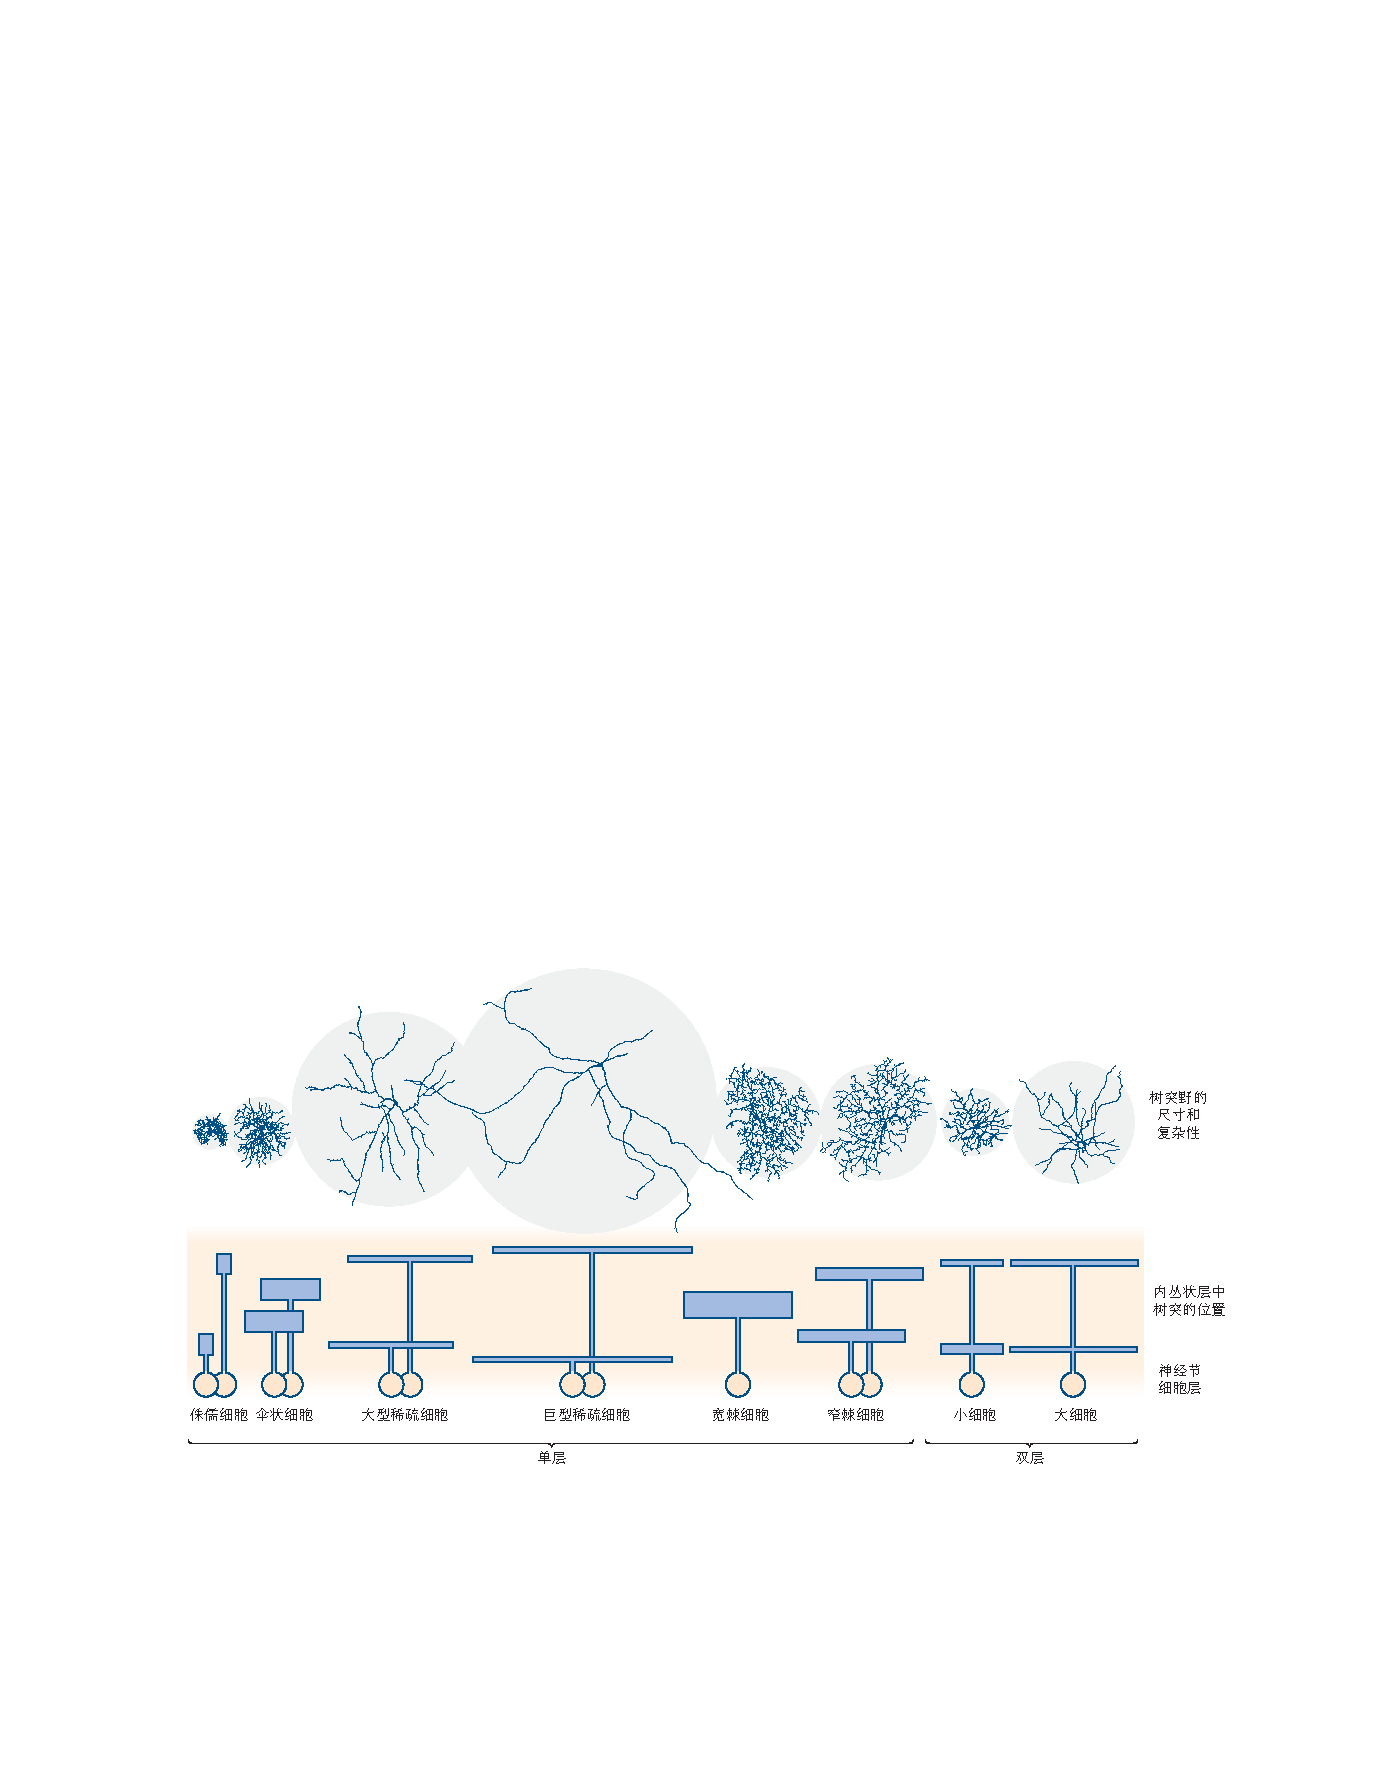
\includegraphics[width=1.0\linewidth]{chap03/fig_3_4}
	\caption{感觉神经元可以细分为功能不同的组。 
		例如,至少有 13 种类型的视网膜神经节细胞是根据它们的树突的大小和形状以及它们接收输入信号的视网膜深度来区分的。 
		内丛状层包含视网膜中间神经元(双极和无长突细胞)和神经节细胞之间的连接。 
		(经许可转载自 Dacey 等人,2003 年。版权所有 © 2003 Elsevier。)}
	\label{fig:3_4}
\end{figure}


\subsection{神经胶质细胞支持神经细胞}
神经胶质细胞的数量远远超过神经元——在脊椎动物中枢神经系统中,神经胶质细胞的数量是神经元的 2 到 10 倍。 
尽管这些细胞的名称源自希腊语中的胶水,但胶质细胞通常不会将神经细胞聚集在一起。 
相反,它们围绕着神经元的细胞体、轴突和树突。 
胶质细胞在形态上不同于神经元; 它们不形成树突和轴突。


胶质细胞在功能上也有所不同。 
尽管它们来自相同的胚胎前体细胞,但它们不具有与神经元相同的膜特性,因此不能被电激发。 
因此,它们不直接参与电信号传递,这是神经细胞的功能。 
然而,它们在允许电信号沿着神经元的轴突快速移动方面发挥了作用,而且它们似乎在引导早期发育过程中的连接以及稳定通过学习发生的神经元之间新的或改变的连接方面发挥了重要作用。 
在过去的十年中,人们对胶质细胞的多种功能的兴趣有所增加,它们的特征已经从支持细胞转变为神经元的功能伙伴(第 \ref{chap:chap7} 章)。


\section{每个神经细胞都是调节特定行为的回路的一部分}
每一种行为都由一组特定的相互连接的神经元介导,而每
一个神经元的行为功能都取决于它与其他神经元的联系。 一个简单的行为,膝跳反射,将说明这一点。 
当身体的短暂不平衡拉伸腿部股四头肌伸肌时,反射开始。 
这种拉伸会产生传送给运动神经元的感觉信息,而运动神经元又会向伸肌发出收缩命令,从而恢复平衡。


这种反射在临床上用于测试神经的完整性以及反射幅度(或增益)的脑脊髓控制。 
潜在的机制很重要,因为它可以维持股四头肌的正常张力,并防止我们的膝盖在站立或行走时屈曲。 
股四头肌的肌腱,一种移动小腿的伸肌,通过髌骨(膝盖骨)的肌腱附着在胫骨上。 
轻敲髌骨正下方的肌腱可以拉伸股四头肌。 
这种拉伸启动股四头肌的反射性收缩,产生熟悉的膝跳。 
通过增加选定肌肉群的张力,牵张反射改变腿的位置,突然向外伸展(图 \ref{fig:3_5})。

\begin{figure}[htbp]
	\centering
	\includegraphics[width=0.5\linewidth]{chap03/fig_3_5}
	\caption{膝跳反射由感觉和运动神经元组成的简单回路控制。 
		用反射锤轻敲膝盖骨,拉动股四头肌的肌腱,股四头肌是延伸小腿的肌肉。
		当肌肉因肌腱的牵拉而伸展时,有关肌肉变化的信息会通过感觉神经元传送到中枢神经系统。 
		在脊髓中,感觉神经元与收缩股四头肌(被拉伸的肌肉)的伸肌运动神经元形成兴奋性突触。 
		感觉神经元通过中间神经元间接作用,抑制屈肌运动神经元,否则这些神经元会收缩相对的腿筋肌肉。 
		这些动作结合起来产生反射行为。 
		在图中,每个伸肌和屈肌运动神经元代表许多细胞群。}
	\label{fig:3_5}
\end{figure}


参与膝跳反射的感觉神经元的细胞体聚集在背根神经节的脊髓附近。 
它们是伪单极细胞; 每个细胞轴突的一个分支延伸到周围的股四头肌,而另一个延伸到脊髓的中央。 
支配股四头肌的分支与拉伸敏感受体(肌梭)接触,并在肌肉拉伸时兴奋。 
到达脊髓的分支与支配股四头肌并控制其收缩的运动神经元形成兴奋性连接。 
该分支还联系抑制控制相对屈肌的运动神经元的局部中间神经元(图 \ref{fig:3_5})。 
尽管这些局部中间神经元本身不参与牵张反射的产生,但它们通过协调相反肌肉群的动作来增加反射的稳定性。 
因此,产生牵张反射的电信号携带四种信息:

1. 感觉信息从肌肉传递到中枢神经系统(脊髓)。

2. 来自中枢神经系统的运动命令被发送到进行膝跳的肌肉。

3. 向支配相反肌肉的运动神经元发出抑制性命令。

4. 与膝跳有关的局部神经元活动的信息被发送到中枢神经系统的更高中枢,允许大脑同时或依次协调不同的行为。

此外,大脑断言对反射的上下文相关控制以调整其增益。 
例如,当我们跑步时,腿筋肌肉会弯曲膝盖,从而拉伸股四头肌。 
大脑和脊髓抑制牵张反射,使股四头肌放松。 
当这些下行路径被破坏时,就像在某些划水动作中一样,反射被放大并且关节变得僵硬。


仅仅拉伸一块肌肉,股四头肌,就会激活数百个感觉神经元,每个神经元与 45 到 50 个运动神经元直接接触。 
这种连接模式,其中一个神经元激活许多目标细胞,称为发散(图 \ref{fig:3_6}A)。 
它在神经系统的输入阶段尤为常见; 通过将其信号分配给许多靶细胞,单个神经元可以发挥广泛而多样的影响。 
相反,膝跳电路中的单个运动细胞从大约 130 个感觉细胞接收 200 到 450 个输入触点。 
这种连接模式称为收敛(图 \ref{fig:3_6}B)。 
它在神经系统的输出阶段很常见; 从许多感觉神经元接收信息的目标运动细胞能够整合来自许多来源的信息。 
每个感觉神经元输入产生相对较弱的兴奋,因此收敛也确保只有当足够数量的感觉神经元一起被激活时,运动神经元才会被激活。


\begin{figure}[htbp]
	\centering
	\includegraphics[width=0.5\linewidth]{chap03/fig_3_6}
	\caption{发散和会聚的神经元连接是大脑的一个关键组织特征。 
		A. 在感觉系统中,每个受体神经元通常与代表第二阶段处理的几个神经元联系。 
		在随后的处理阶段,传入的连接更加分散。 
		这使得来自单个站点的感觉信息可以更广泛地分布在脊髓和大脑中。 
		B. 相比之下,运动神经元是逐渐融合连接的目标。 
		通过这种安排,需要来自许多突触前细胞的输入来激活运动神经元。}
	\label{fig:3_6}
\end{figure}


诸如膝跳反射之类的牵张反射是由在兴奋性突触处连接的两类神经元产生的一种简单行为。 
但并非大脑中的所有重要信号都是兴奋性的。 
许多神经元会产生抑制信号,从而降低放电的可能性。 
即使在简单的膝跳反射中,感觉神经元也会产生兴奋性和抑制性连接。 
腿部伸肌中的兴奋性连接会导致这些肌肉收缩,而与抑制性中间神经元的连接会阻止拮抗性屈肌收缩。 
电路的这个特性是前馈抑制的一个例子(图 \ref{fig:3_7}A)。 
在膝跳反射中,前馈抑制是相互的,确保屈肌和伸肌通路始终相互抑制,以便只招募适合运动的肌肉,而不是那些反对运动的肌肉。

\begin{figure}[htbp]
	\centering
	\includegraphics[width=0.5\linewidth]{chap03/fig_3_7}
	\caption{抑制性中间神经元可以产生前馈或反馈抑制。 
		A. 前馈抑制通过抑制调节相反作用的通路的活性来增强活性通路的效果。 
		前馈抑制在单突触反射系统中很常见。 
		例如,在膝跳反射回路(图 3-5)中,来自伸肌的传入神经元不仅会刺激伸肌运动神经元,还会刺激抑制性中间神经元,从而阻止神经支配相对屈肌的运动细胞的放电。 
		B. 反馈抑制是一种自我调节机制。 
		在这里,伸肌运动神经元作用于抑制性中间神经元,后者反过来作用于伸肌运动神经元本身,从而降低它们放电的可能性。 
		其作用是抑制受刺激通路内的活动并防止其超过某个临界水平。}
	\label{fig:3_7}
\end{figure}


一些电路提供反馈抑制。 
例如,运动神经元可能与肌肉和抑制性中间神经元都有兴奋性连接,后者本身与运动神经元形成连接。 
当抑制性中间神经元被运动神经元兴奋时,中间神经元能够限制运动神经元兴奋肌肉的能力(图 \ref{fig:3_7}B)。 
当我们在后面的章节中研究更复杂的行为时,我们会遇到许多前馈和反馈抑制的例子。


\section{信号在所有神经细胞中的组织方式相同}
为了产生一种行为,例如牵张反射,每个参与的感觉和运动神经细胞必须依次产生四种不同的信号,每个信号位于细胞内的不同位置。 
尽管细胞大小和形状、递质生物化学或行为功能各不相同,但几乎所有神经元都可以用一个模型神经元来描述,该模型神经元具有产生四种类型信号的四个功能组件:
一个用于产生分级输入信号的接收组件,一个求和或 产生触发信号的综合组件,产生全或无传导信号的传导远程信号组件,以及产生输出信号到下一个神经元或肌肉或腺体细胞的突触组件(图 \ref{fig:3_8})。

\begin{figure}[htbp]
	\centering
	\includegraphics[width=0.5\linewidth]{chap03/fig_3_8}
	\caption{大多数神经元有四个功能区域,在这些区域中会生成不同类型的信号。 
		因此,大多数神经元的功能组织,无论类型如何,都可以用模型神经元示意性地表示。 
		该模型神经元是 Ramón y Cajal 动态极化原理的生理表达。 
		输入信号、综合信号和传导信号都是电信号,对细胞来说是不可或缺的,而输出信号是由细胞射入突触间隙的化学物质。 
		并非所有神经元都具有所有这些特征。 
		例如,一些局部中间神经元缺乏导电成分。}
	\label{fig:3_8}
\end{figure}


神经元中产生的不同类型的信号部分取决于细胞膜的电特性。 
当细胞处于静止状态时,包括神经元在内的每个细胞都在质膜两侧保持一定的电位差。 
这称为静息膜电位。 
在典型的静息神经元中,细胞内部的电压比细胞外部的电压负大约 65 mV。 
因为膜外电压被定义为零,所以我们说静息膜电位为 –65 mV。 
不同神经细胞的静息电位范围为 –40 至 –80 mV; 
在肌肉细胞中,它更大,约为 –90 mV。 
正如第 \ref{chap:chap9} 章中详细描述的,静息膜电位由两个因素造成:带电离子的不均匀分布,特别是带正电的 Na+ 和 K+ 离子,以及膜的选择性渗透性。


带正电的离子在细胞膜两侧的不均匀分布由两个主要机制维持。 
细胞内 Na+ 和 K+ 浓度主要由膜蛋白控制,膜蛋白主动将 Na+ 泵出细胞并将 K+ 泵回细胞内。 
这个 Na+-K+ 泵,我们将在第 \ref{chap:chap9} 章中详细了解,它使细胞内的 Na+ 浓度保持在较低水平(约为细胞外浓度的十分之一),并使 K+ 浓度保持在较高水平(约为细胞外浓度的 20 倍)。 
Na+ 和 K+ 的细胞外浓度由肾脏和星形胶质细胞(也称为星形胶质细胞)维持。


否则不可渗透的细胞膜含有形成称为离子通道的孔的蛋白质。 细胞静止时活跃的通道对 K+ 的渗透性很高,但对 Na+ 的渗透性要低得多。 
K+ 离子往往会沿着离子的浓度梯度从这些开放通道中泄漏出来。 
当 K+ 离子离开细胞时,它们会在膜的内表面留下一团未中和的负电荷,因此膜内的净电荷比膜外的负电荷更多。 
在这种情况下,相对于神经元外部,膜电位通常保持在 –65 mV 左右,据说神经元处于静止状态。


当细胞开始吸收细胞外浓度较高的 Na+(或 Ca2+)时,静息状态就会受到干扰。 
这些带正电的离子向内运动(内向电流)部分地中和了电池内部的负电压。 
我们将在下面详细介绍这些事件。 
然而,接下来发生的事情是理解神经元是什么使信号适合传递信息的关键。


当一个细胞,如神经和肌肉,其膜电位可以迅速而显着地改变时,就被认为是可兴奋的。 
在许多神经元中,膜电位 10 mV 的变化(从 –65 到 –55 mV)使膜对 Na+ 的渗透性比对 K+ 的渗透性强得多。 
由此产生的 Na+ 流入进一步中和了细胞内的负电荷,导致对 Na+ 的渗透性更高。 
结果是膜电位发生短暂的爆炸性变化,变为 +40 mV,即动作电位。 
这种电位被积极地沿着细胞的轴突传导到轴突的末端,在那里它启动与突触后神经元或肌肉细胞的精细化学相互作用。 
由于动作电位是主动传播的,因此其振幅在到达轴突末端时不会减小。 
动作电位通常持续约 1 毫秒,之后膜恢复到其静止状态,电荷正常分离,对 K+ 的渗透性高于对 Na+ 的渗透性。


静息电位和动作电位的潜在机制在第 \ref{chap:chap9} 章和第 \ref{chap:chap10} 章中详细讨论。
除了动作电位代表的长距离信号外,神经细胞还产生局部信号——受体电位和突触电位——这些信号不活跃 传播并且通常在几毫米内衰减(见下一节)。


产生远程和局部信号的膜电位变化可以是静息电位的降低或增加。 
也就是说,静息膜电位是所有信号发生的基线。 
膜电位的降低(称为去极化)增强了细胞产生动作电位的能力,因此具有兴奋性。 
相反,膜电位的增加,称为超极化,使细胞不太可能产生动作电位,因此具有抑制作用。


\subsection{输入组件产生分级本地信号}
在大多数静止的神经元中,没有电流从细胞的一部分流向另一部分,因此静息电位始终相同。 
在感觉神经元中,电流通常由物理刺激启动,物理刺激会激活神经元接受表面的特殊受体蛋白。 
在我们膝跳反射的例子中,肌肉的拉伸会激活特定的离子通道,这些离子通道会响应感觉神经元膜的拉伸而打开,我们将在第 \ref{chap:chap18} 章中了解到。
当细胞被拉伸时,这些通道的打开允许 Na+ 离子快速流入感觉细胞。 
这种离子电流改变膜电位,产生称为受体电位的局部信号。


受体电位的幅度和持续时间取决于肌肉拉伸的强度:拉伸越大或持续时间越长,由此产生的受体电位越大或持续时间越长(图 \ref{fig:3_9}A)。 
也就是说,受体电位是分级的,这与 allor-none 动作电位不同。 
大多数受体电位是去极化的(兴奋性的); 在视网膜中发现超极化(抑制)受体电位。

\begin{figure}[htbp]
	\centering
	\includegraphics[width=1.0\linewidth]{chap03/fig_3_9}
	\caption{神经元的四个信号成分中的每一个都会产生一个特征信号。 
		该图显示了通过肌肉拉伸激活的感觉神经元,神经元通过专门的受体(肌梭)感知。 
		A. 输入信号,称为受体电位,在振幅和持续时间上分级,与刺激的振幅和持续时间成正比。 
		B. 触发区总结了受体电位产生的去极化。 
		只有当受体电位超过某个电压阈值时才会产生动作电位。 
		一旦超过这个阈值,受体电位幅度的任何进一步增加只能增加动作电位产生的频率,因为动作电位具有恒定的幅度。 
		受体电位的持续时间决定了动作电位序列的持续时间。 
		因此,受体电位的分级振幅和持续时间被转化为触发区产生的动作电位中的频率代码。 
		产生的所有动作电位都忠实地沿着轴突传播。 
		C. 动作电位是全有或全无。 
		因为所有动作电位都具有相似的幅度和持续时间,所以放电的频率和持续时间编码了信号所携带的信息。 
		D. 当动作电位到达突触末梢时,它会启动神经递质的释放,即用作输出信号的化学物质。 
		突触前细胞中动作电位的频率决定了细胞释放多少神经递质。}
	\label{fig:3_9}
\end{figure}

受体电位是在神经系统中编码的第一个拉伸表示。 
然而,由于这种去极化从拉伸感受器被动传播,它不会传播很远。 
如果轴突的直径较大,则距离较长,如果直径较小,则距离较短。 
此外,如果电流可以轻松通过膜,则距离会更短,如果膜被髓磷脂绝缘,则距离会更长。 
因此,来自拉伸感受器的感受器电位仅移动 1 至 2 毫米。 
事实上,就在 1 毫米远的地方,信号的幅度仅为产生位置的三分之一左右。 
为了成功地传送到脊髓,局部信号必须被放大——它必须产生动作电位。 
在膝跳反射中,如果感觉神经元中的受体电位到达轴突中朗飞的第一个节点并且足够大,它将触发动作电位(图 \ref{fig:3_9}B),然后无故障地传播到轴突 脊髓中的末端(图 \ref{fig:3_9}C)。 
在感觉神经元和运动神经元之间的突触处,动作电位会产生一系列事件,这些事件会导致运动神经元的输入信号。


在膝跳反射中,感觉神经元突触前末梢的动作电位启动化学物质或神经递质释放到突触间隙(图 \ref{fig:3_9}D)。 
扩散穿过裂隙后,递质与运动神经元突触后膜中的受体蛋白结合,从而直接或间接打开离子通道。 
随后的电流流动会短暂地改变运动细胞的膜电位,这种变化称为突触电位。


与受体电位一样,突触电位也是分级的; 
它的振幅取决于释放发射器的量。 
在同一细胞中,突触电位可以去极化或超极化,具体取决于被激活的受体分子的类型。 
突触电位,如受体电位,被动传播。 
因此,电位的变化将保持局部,除非信号超出轴突的初始段,在那里它可以产生动作电位。 
一些树突并非完全被动,而是包含促进突触电位的特化,从而提高其产生动作电位的功效(第 \ref{chap:chap13} 章)。 
表 3-1 总结了受体和突触电位的特征。


\subsection{触发区决定产生动作电位}
谢林顿首先指出,神经系统的功能是权衡不同类型信息的后果,然后决定适当的反应。 
神经系统的这种整合功能在神经元触发区(轴突的初始部分)的事件中清晰可见。


动作电位是由 Na+ 通过细胞膜中的通道突然流入而产生的,这些通道响应于膜电位的变化而打开和关闭。 
当输入信号(受体电位或突触电位)使膜区域去极化时,膜电位的局部变化会打开局部 Na+ 通道,使 Na+ 沿着其浓度梯度从 Na+ 浓度高的细胞外流到细胞内 它低的地方。


由于轴突的起始段具有最高密度的电压敏感 Na+ 通道,因此产生动作电位的阈值最低,因此沿细胞膜被动传播的输入信号更有可能在起始段产生动作电位 轴突的部分比在细胞中的其他部位。 
因此,这部分轴突被称为触发区。 
所有受体(或突触)电位的活动都在这里求和,如果输入信号的总和达到阈值,神经元就会产生动作电位。


\subsection{导电成分传播全有或全无动作电位}
动作电位是全有或全无:低于阈值的刺激不会产生信号,但高于阈值的刺激都会产生相同幅度的信号。 
无论刺激强度或持续时间的变化如何,每个动作电位的幅度和持续时间几乎相同,这适用于沿着有髓轴突的朗飞节点处的每个再生动作电位。 
此外,与被动传播和振幅减小的受体和突触电位不同,正如我们所见,动作电位在沿着轴突到达其目标(距离可达 1 米)时不会衰减。 
因为它是周期性再生的。 
这种传导信号可以以高达 100 m/s 的速度传播。 
事实上,动作电位的显着特征是它们是高度刻板的,从一个神经细胞到另一个神经细胞的变化很小(但在某些情况下很重要)。 
埃德加·阿德里安 (Edgar Adrian) 在 1920 年代证明了这一特征,他是最早在细胞水平上研究神经系统的人之一。 
阿德里安发现所有动作电位都具有相似的形状或波形(见图 \ref{fig:3_2})。 
由感觉轴突带入神经系统的动作电位与由运动轴突从神经系统带入肌肉的动作电位通常无法区分。


传导信号只有两个特征传达信息:动作电位的数量和它们之间的时间间隔(图 \ref{fig:3_9}C)。 
正如阿德里安 (Adrian) 在 1928 年总结他对感觉纤维的研究时所说:“所有的冲动都非常相似,无论信息是注定要引起光感、触感还是痛感; 如果它们挤在一起,感觉就会强烈,如果它们相距很远,感觉就会相应地微弱。” 
因此,决定感觉强度或运动速度的是动作电位的频率。 
同样,感觉或运动的持续时间由产生动作电位的时间段决定。


除了动作电位的频率,动作电位的模式也传达了重要的信息。 
例如,一些神经元在没有刺激的情况下会自发活跃。 
一些自发活跃的神经细胞(跳动的神经元)有规律地激发动作电位; 其他人(爆发的神经元)在短暂的动作电位爆发中发射。 
这些不同的细胞对相同的兴奋性突触输入有不同的反应。 
兴奋性突触电位可能会在一个非自发活跃的细胞中启动一个或多个动作电位,而对自发活跃细胞的相同输入只会增加现有的放电率。


当输入信号具有抑制性时,会出现更显着的差异。 抑制性输入在沉默细胞中几乎没有信息价值。 
相比之下,在自发活跃的细胞中,抑制可以起到强大的塑造作用。 
通过在其他正在进行的活动中建立沉默期,抑制可以在不存在的地方产生一种复杂的交替放电和沉默模式。 
放电模式的这种细微差异可能对神经元之间的信息传递产生重要的功能影响。 
神经元网络的数学建模者试图描述神经代码,其中信息也由细粒度的放电模式——每个动作电位的确切时间——携带。


如果信号是固定的并且仅反映刺激的最基本属性,那么它们如何携带复杂行为所需的丰富信息呢? 
如何将包含蜜蜂视觉信息的信息与包含蜜蜂蜇伤疼痛信息的信息区分开来?
这些感觉信号与自主运动的运动信号有何区别? 
答案很简单,但却是神经系统最重要的组织原则之一:
相互连接的神经元形成解剖学和功能上不同的通路——标记线——正是这些连接神经元的通路,这些标记线,而不是单个神经元,传达 信息。 
视网膜中对光有反应的受体细胞激活的神经通路与皮肤中对触觉有反应的感觉细胞激活的神经通路完全不同。


\subsection{输出组件释放神经递质}
当动作电位到达神经元的末端时,它会刺激细胞释放化学物质。 
这些物质称为神经递质,可以是有机小分子,例如 L-谷氨酸和乙酰胆碱,也可以是肽,例如 P 物质或 LHRH(促黄体激素释放激素)。


神经递质分子存在于称为突触小泡的亚细胞器中,突触小泡聚集在轴突末端的特殊释放部位,称为活性区。 
为了将它们的递质物质喷射到突触间隙中,囊泡向上移动并与神经元的质膜融合,然后通过已知的过程突然打开以将递质释放到突触间隙(突触前细胞和突触后细胞之间的细胞外空间)中 作为胞吐作用。 
第 \ref{chap:chap14} 章和第 \ref{chap:chap15} 章描述了神经递质释放的分子机制。


释放的神经递质分子是神经元的输出信号。 
因此,输出信号根据释放的递质量进行分级,递质量由到达突触前末梢的动作电位的数量和频率决定(图 \ref{fig:3_9}C,D)。 
释放后,递质分子扩散穿过突触间隙并与突触后神经元上的受体结合。 
这种结合导致突触后细胞产生突触电位。 
突触电位是否具有兴奋或抑制作用取决于突触后细胞中受体的类型,而不取决于特定的化学神经递质。 
相同的递质物质在不同的受体上可能有不同的作用。


\subsection{牵张反射通路说明了神经信号从感觉到运动的转变}
正如我们所见,当信号从神经元的一个组成部分移动到另一个组成部分或在神经元之间移动时,信号的属性会发生变化。 
在牵张反射中,当肌肉被拉伸时,刺激的幅度和持续时间反映在感觉神经元中产生的受体电位的幅度和持续时间中(图 \ref{fig:3_10}A)。 
如果受体电位超过该细胞中动作电位的阈值,则分级信号会在触发区转换为动作电位。
尽管个体动作电位是全有或全无信号,但受体电位超过阈值越多,去极化越大,因此轴突中动作电位的频率就越高。 
输入信号的持续时间也决定了动作电位序列的持续时间。

\begin{figure}[htbp]
	\centering
	\includegraphics[width=1.0\linewidth]{chap03/fig_3_10}
	\caption{产生反射动作的信号序列。 
		A. 肌肉的拉伸会在专门的受体(肌梭)中产生受体电位。 
		受体电位的幅度与拉伸强度成正比。 
		这种势能被动地传播到朗飞第一个节点的综合区或触发区。 
		如果受体电位足够大,它会触发动作电位,然后沿着轴突主动传播而不会发生变化,直至轴突末端。 
		在终端的特定位置,动作电位导致化学神经递质(输出信号)的释放。 
		递质扩散穿过轴突末端和支配拉伸肌肉的目标运动神经元之间的突触间隙; 
		然后它与运动神经元外膜上的受体分子结合。 
		B. 这种相互作用启动了一个被动传播到运动神经元轴突触发区的突触电位,在那里它启动了一个主动传播到运动神经元轴突末端的动作电位。 
		在轴突末端,动作电位导致肌肉纤维附近神经递质的释放。 
		C. 神经递质结合肌纤维上的受体,产生突触电位。 
		突触电位触发肌肉中的动作电位,从而引起收缩。}
	\label{fig:3_10}
\end{figure}


由放电频率和持续时间编码的信息沿着轴突忠实地传递到其末端,在那里动作电位的放电决定了发射器的释放量。 
这些信号阶段在运动神经元(图 \ref{fig:3_10}B)和肌肉(图 \ref{fig:3_10}C)中有对应的阶段。


\section{神经细胞在分子水平上的差异最大}
我们概述的神经元信号模型是一种适用于大多数神经元的简化模型,但也有一些重要的变化。 
例如,一些神经元不产生动作电位。 
这些通常是没有导电成分的局部中间神经元; 它们没有轴突或轴突太短以至于不需要信号的再生。 
在这些神经元中,输入信号被汇总并被动传播到释放递质附近的突触前末梢区域。 
自发活跃的神经元不需要感觉或突触输入来激发动作电位,因为它们具有一类特殊的离子通道,即使在没有兴奋性突触输入的情况下也允许 Na+ 电流流动。


即使是形态相似的细胞在分子细节上也可能存在重大差异。 
例如,它们可以具有不同的离子通道组合。 
正如我们将在第 \ref{chap:chap10} 章中了解到的,不同的离子通道为神经元提供了不同的阈值、兴奋特性和放电模式。 
这样的神经元可以将突触电位编码成不同的放电模式,从而传达不同的信息。


神经元在用作递质的化学物质和从其他神经元接收递质物质的受体方面也有所不同。 
事实上,许多作用于大脑的药物都是通过改变特定化学递质或受体的作用来实现的。 
由于神经元之间的生理差异,一种疾病可能影响一类神经元而不影响其他神经元。 
某些疾病只影响运动神经元(肌萎缩侧索硬化症和脊髓灰质炎),而其他疾病主要影响感觉神经元(麻风病和脊髓灰质炎,梅毒晚期)。 
帕金森病是一种随意运动障碍,会损害一小部分使用多巴胺作为神经递质的神经元。 
有些疾病甚至在神经元内也具有选择性,仅影响感受元件、细胞体或轴突。 
在第 \ref{chap:chap57} 章中,我们描述了对重症肌无力(一种由肌肉膜中有缺陷的递质受体引起的疾病)的研究如何为突触传递提供了重要的见解。 
事实上,由于神经系统在分子水平上有如此多的细胞类型和变异,它比身体的任何其他器官系统更容易患上更多的疾病(精神病学和神经学)。


尽管神经细胞之间存在形态差异,但电信号的分子机制却惊人地相似。 
这种简单性是幸运的,因为了解一种神经细胞中信号传导的分子机制有助于理解许多其他神经细胞中的这些机制。


\section{反射回路是理解行为神经结构的起点}
牵张反射说明了几种类型的神经细胞之间的相互作用如何构成一个产生简单行为的功能回路,即使涉及的神经元数量很大(牵张反射回路可能有几百个感觉神经元和一百个运动神经元) 神经元)。 
一些无脊椎动物能够使用少得多的神经元做出与反射一样复杂的行为。 
此外,在某些情况下,仅一个关键命令神经元就可以触发复杂的行为,例如从有害刺激中撤回身体部位。


对于更复杂的行为,尤其是高等脊椎动物,需要许多神经元,但通常会保留简单反射的基本神经结构。 
首先,通常有一组可识别的神经元,其放电率会随着特定类型的环境刺激而变化,例如特定频率的音调,或特定角度的明暗并置。 
正如牵张感受器神经元的放电率编码肌肉紧张程度,皮层感觉区域的皮质神经元放电率编码感觉特征的强度(例如,轮廓的对比度)。 
正如我们将在后面的章节中看到的那样,仅通过改变一小组神经元的放电率就可以改变知觉的特征。


其次,通常有一组可识别的神经元,其放电率在动物执行运动动作之前发生变化。 
正如运动神经元的尖峰率控制股四头肌收缩的幅度——因此膝反射——运动皮层神经元的放电率也影响将要进行的运动的潜伏期和类型。 
这些神经元究竟对运动的哪个方面进行了编码仍然是一个活跃的研究领域,但已经确定的是,神经元组通过调整其放电率以分级方式影响随后的动作。 
在大脑皮层的其他关联区域,神经元的分级放电率编码对思维过程至关重要的数量,例如与选择相关的证据数量(第 \ref{chap:chap56} 章)。


尽管复杂的心理操作比简单的牵张反射复杂得多,但考虑认知功能在多大程度上受到以类似于简单反射的任何方式组织的神经机制的支持,可能证明是有用的。 
调解复杂的行为和思想可能需要哪些类型的阐述? 
与具有复杂行为的简单反射不同,感觉神经元的激活不会立即引起反射动作。 
这个过程有更多的偶然性。 
尽管简单的反应受上下文调节,但心理功能更受复杂的突发事件的影响,考虑到任何一种刺激的许多可能影响以及任何一种行为的许多可能的沉淀物。 
鉴于这些突发事件,我们不得不设想在大脑的数据采集系统(不仅是感觉系统,还有记忆系统)和效应器系统之间建立灵活的路由。 
正如我们将在后面的章节中看到的那样,这是大脑皮层的高级联合区域的作用,与几个皮层下脑结构协同作用。


也许复杂的心理功能和反射之间更显着的区别是行动的时机。 
一旦被激活,反射回路几乎会在感官刺激后立即采取行动。 
任何延迟主要取决于反射的传入和传出肢体中动作电位的传导速度(例如,踝反射比膝反射慢,因为脊髓离小腿肌肉的牵张感受器比它离小腿肌肉的牵拉感受器更远) 来自大腿伸肌)。 
对于更复杂的行为,动作不需要随着感官信息的到达而或多或少地立即发生。 它可能会延迟等待其他信息或仅在特定情况发生时才表达。


有趣的是,灵长类动物皮层联合区的神经元有能力在数秒内维持分级放电率。 
这些神经元大量存在于调节感觉和运动区域之间灵活联系的大脑区域。 
它们提供了摆脱反射行为的瞬时性质的自由,因此可以提供将认知功能与更直接的感觉运动转换(如反射)区分开来的基本电路特性。


\section{神经回路可以通过经验进行修改}
学习可以导致持续数年甚至一生的行为改变。 
但即使是简单的反应也可以改变,尽管时间要短得多。 
许多行为可以通过学习来改变这一事实提出了一个有趣的问题:如果神经系统连接得如此精确,那么行为是如何改变的呢? 
当信号单元(神经元)之间的连接在早期发育过程中设置时,行为的神经控制如何发生变化?


针对这一困境,已经提出了几种解决方案。 
最有远见的提议是可塑性假说,该假说由拉蒙·卡哈尔 (Ramón y Cajal) 在 20 世纪之交首次提出。 
波兰心理学家 Jerzy Konorski 于 1948 年提出了这一假设的现代形式。


刺激的应用导致神经系统发生双重变化……[T]第一个特性,神经细胞据此对传入的冲动做出反应……我们称之为兴奋性,并且……由于这个特性而产生变化…… 我们称由于兴奋性而产生的变化。 
第二个属性,由于适当的刺激或它们的组合,特定的神经元系统中会出现某些永久的功能转换,我们将称之为可塑性和相应的变化可塑性变化。


现在有相当多的证据表明化学突触的功能可塑性。 
这些突触通常具有显着的短期生理变化(持续几秒到几小时)的能力,这些变化会增加或减少突触的有效性。 
长期的生理变化(持续数天或更长时间)会引起解剖学改变,包括突触的修剪甚至新突触的生长。 
正如我们将在后面的章节中看到的那样,化学突触在早期发育的关键时期以及整个生命过程中都会在功能和解剖学上发生变化。 
神经元的这种功能可塑性赋予我们每个人与周围自然和社会世界互动的独特方式。



\section{亮点}
1. 神经细胞是神经系统的信号单位。 信号主要是细胞内的电信号和细胞之间的化学信号。 
尽管大小和形状各不相同,但神经细胞具有某些共同特征。 
每个人都有专门的受体或传感器,分别接收来自其他神经细胞或感官的输入; 
一种将输入转换为电信号的机制; 产生全或无电脉冲的阈值机制,即动作电位,可以沿着将神经细胞连接到其突触目标(另一个神经细胞、肌肉或腺体)的轴突再生; 以及产生影响目标的化学物质(神经递质)释放的能力。


2.胶质细胞支持神经细胞。 
一种类型提供绝缘,可加速动作电位沿轴突的传播。 
其他帮助建立神经细胞运作的化学环境,还有一些将神经活动与神经系统的血管供应联系起来。


3. 神经细胞的形态、它们建立的联系以及它们建立的位置不同。 
这在视网膜等特殊结构中最为明显。 
也许神经元之间最大的差异是在分子水平上。 
分子多样性的例子包括不同受体的表达、用于合成不同神经递质的酶以及离子通道的不同表达。 
基因表达的差异为理解为什么某些疾病影响某些神经元而不影响其他神经元提供了起点。


4. 每个神经细胞都是具有一种或多种行为功能的回路的一部分。 
牵张反射电路是一个简单电路的例子,它会产生响应刺激的行为。 
它的简单性掩盖了综合功能,例如放松对抗拉伸肌肉的肌肉。


5. 现代神经科学渴望解释比反射复杂得多的心理过程。 
一个自然的起点是理解必须详细说明电路以支持感觉运动转换的方式,这与反射不同,它是偶然的、灵活的,并且不受制于即时的感觉处理和运动控制。


6. 神经连接可以根据经验进行修改。 
在简单的电路中,这个过程是神经元之间连接强度的简单变化。 
现代神经科学的一个工作假设是,在简单电路中发挥作用的“可塑性”机制在学习更复杂的行为和认知功能方面也发挥着关键作用。


\section{选读}

\section{参考文献}













\chapter{神经回路介导行为的神经解剖学基础} \label{chap:chap4}
人脑以当前计算机无法开始的方式执行操作。 
仅仅是看——看世界并识别一张脸或面部表情——就需要惊人的计算成就。 
事实上,我们所有的感知能力——看、听、闻、尝和触——都是分析的胜利。 
同样,我们所有的自愿行动都是工程学的胜利。 
感觉和运动虽然本身很奇妙,但与形成记忆或理解社会习俗等复杂的认知行为相比就显得苍白无力了。


大脑完成这些计算壮举是因为它的神经细胞在非常精确的功能回路中连接在一起。 
大脑是分层组织的,因此在一个级别处理的信息被传递到更高级别的电路,以进行更复杂和精细的处理。 
从本质上讲,大脑是一个网络的网络。 
不同的大脑区域以整合的方式工作以完成有目的的行为。


在本章中,我们概述了一些回路的神经解剖结构,这些回路使大脑能够处理感觉输入并产生运动输出。 
我们将触觉作为一种感觉方式来关注,因为体感系统特别容易理解,并且因为触觉清楚地说明了从脊髓到大脑皮层的多个级别的感觉处理回路的相互作用。 
我们在这里的目的是说明电路如何控制行为的基本原理。 
在下一章中,我们将考虑这些电路的功能特性,包括它们处理信息的计算。 
在随后的章节中,我们将更详细地讨论各种感觉方式的解剖结构和功能,以及感觉输入如何调节运动。


最后,我们提供了大脑回路的预览,这些回路有助于产生我们日常生活的记忆,称为外显记忆(见第 \ref{chap:chap52} 章和第 \ref{chap:chap54} 章)。 
我们这样做是为了说明,虽然记忆回路中的许多神经元与感觉和运动回路中的神经元相似,但并非所有神经元都相似。 
此外,记忆系统中电路之间通路的组织与运动和感觉系统中的不同。 
这突出了一个基本的神经生物学原则,即大脑的不同回路已经进化出一个组织,以最有效地执行特定功能。


理解大脑的功能组织乍一看似乎令人生畏。 
但正如我们在前一章中看到的那样,大脑的组织通过三个解剖学考虑得到了简化。 
首先,神经元的种类相对较少。 
成千上万的脊髓运动神经元或数百万个新皮质锥体细胞中的每一个都具有相似的解剖结构并具有相似的功能。 
其次,大脑和脊髓中的神经元聚集在称为核或大脑皮层离散区域的功能组中,形成网络或功能系统。 
第三,大脑皮层的离散区域专门负责感觉、运动或记忆等联想功能。


\section{局部回路执行特定的神经计算,这些计算被协调以调制复杂的行为}

神经元相互连接形成功能电路。 
例如,在脊髓内,简单的反射回路接收来自拉伸感受器的感觉信息,并将输出发送到各个肌肉群。 
对于更复杂的行为功能,信息处理的不同阶段在神经系统不同区域的网络中进行。 
神经系统内神经元之间的连接可以有不同的长度。


在大脑区域内,可能是兴奋性或抑制性的局部连接将许多神经元整合到功能网络中。 
这样的局部网络然后可以通过更长的投射向一个或多个其他大脑区域提供输出。 
许多这些较长的路径都有名称。 
例如,从丘脑的外侧膝状体核到视觉皮层的投射称为视辐射。 
从大脑的一侧到大脑另一侧的新皮质(大脑皮层中最靠近大脑表面的区域)的连接形成了胼胝体。 
这些长路径携带的信息整合了许多本地电路的输出(图 \ref{fig:4_1})。

\begin{figure}[htbp]
	\centering
	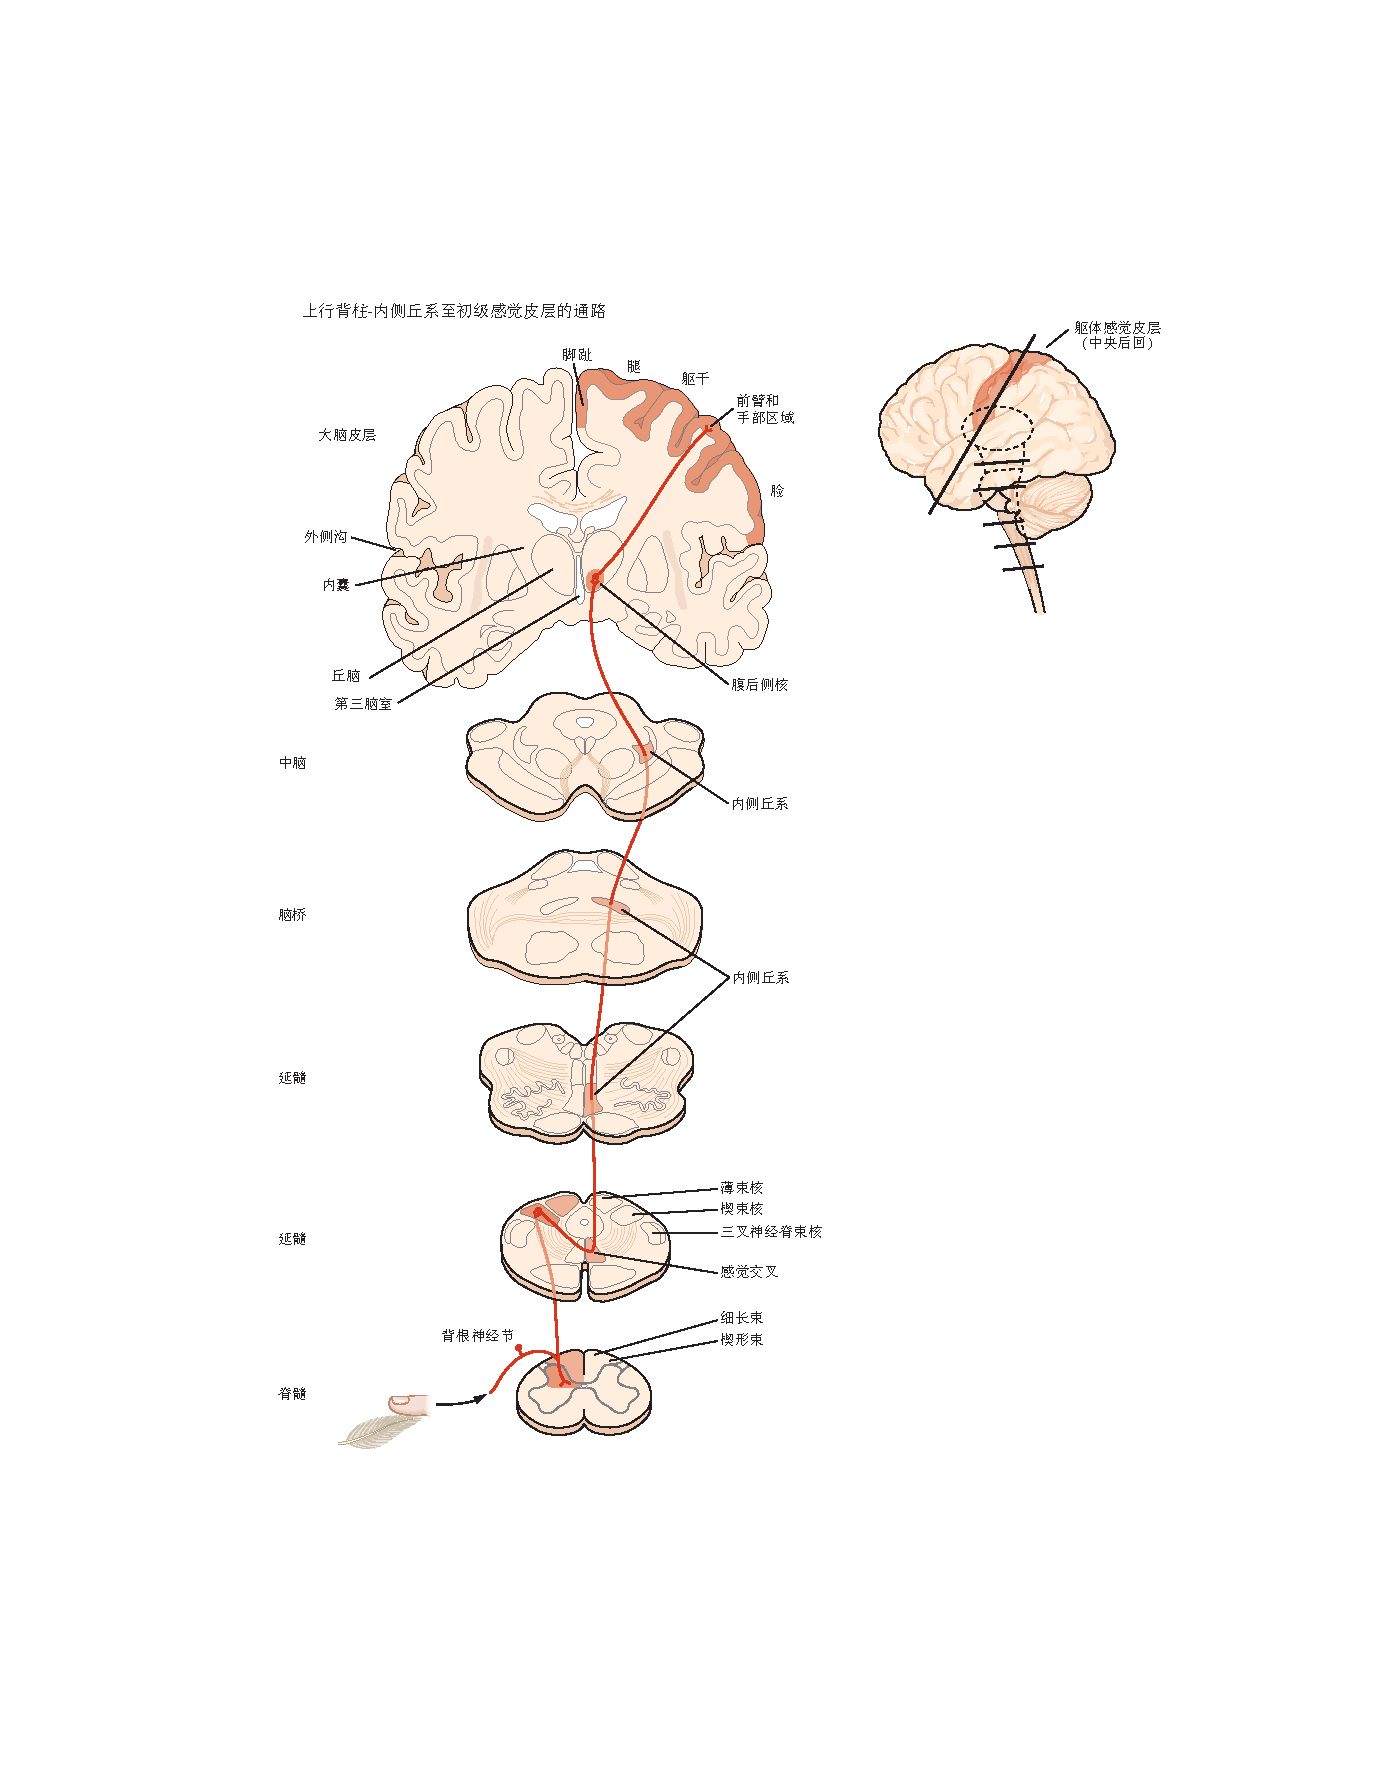
\includegraphics[width=1.0\linewidth]{chap04/fig_4_1}
	\caption{背柱-内侧丘系通路是体感信息的主要传入通路。 
		体感信息通过背根神经节细胞进入中枢神经系统。 
		信息流最终通向体感皮层。 
		传递来自身体不同部位信息的纤维彼此保持有序的关系,并在每个突触传递处以其终止模式形成体表的神经图谱。}
	\label{fig:4_1}
\end{figure}


考虑一下击打网球的简单动作(图 \ref{fig:4_2})。 
在视觉系统中分析有关接近球运动的视觉信息,视觉系统本身是一个分层组织的系统,从视网膜延伸到丘脑的外侧膝状体核,再到枕叶和颞叶的数十个皮质区域(第 \ref{chap:chap21} 章)。
此信息在运动皮层中与有关手臂、腿和躯干位置的本体感受信息相结合,以计算拦截球所需的运动。 
一旦开始挥杆,其他专门负责运动的大脑区域(例如小脑)就会根据关于接近的球的轨迹和手臂位置的源源不断的感官信息,对运动程序进行许多细微的调整。

\begin{figure}[htbp]
	\centering
	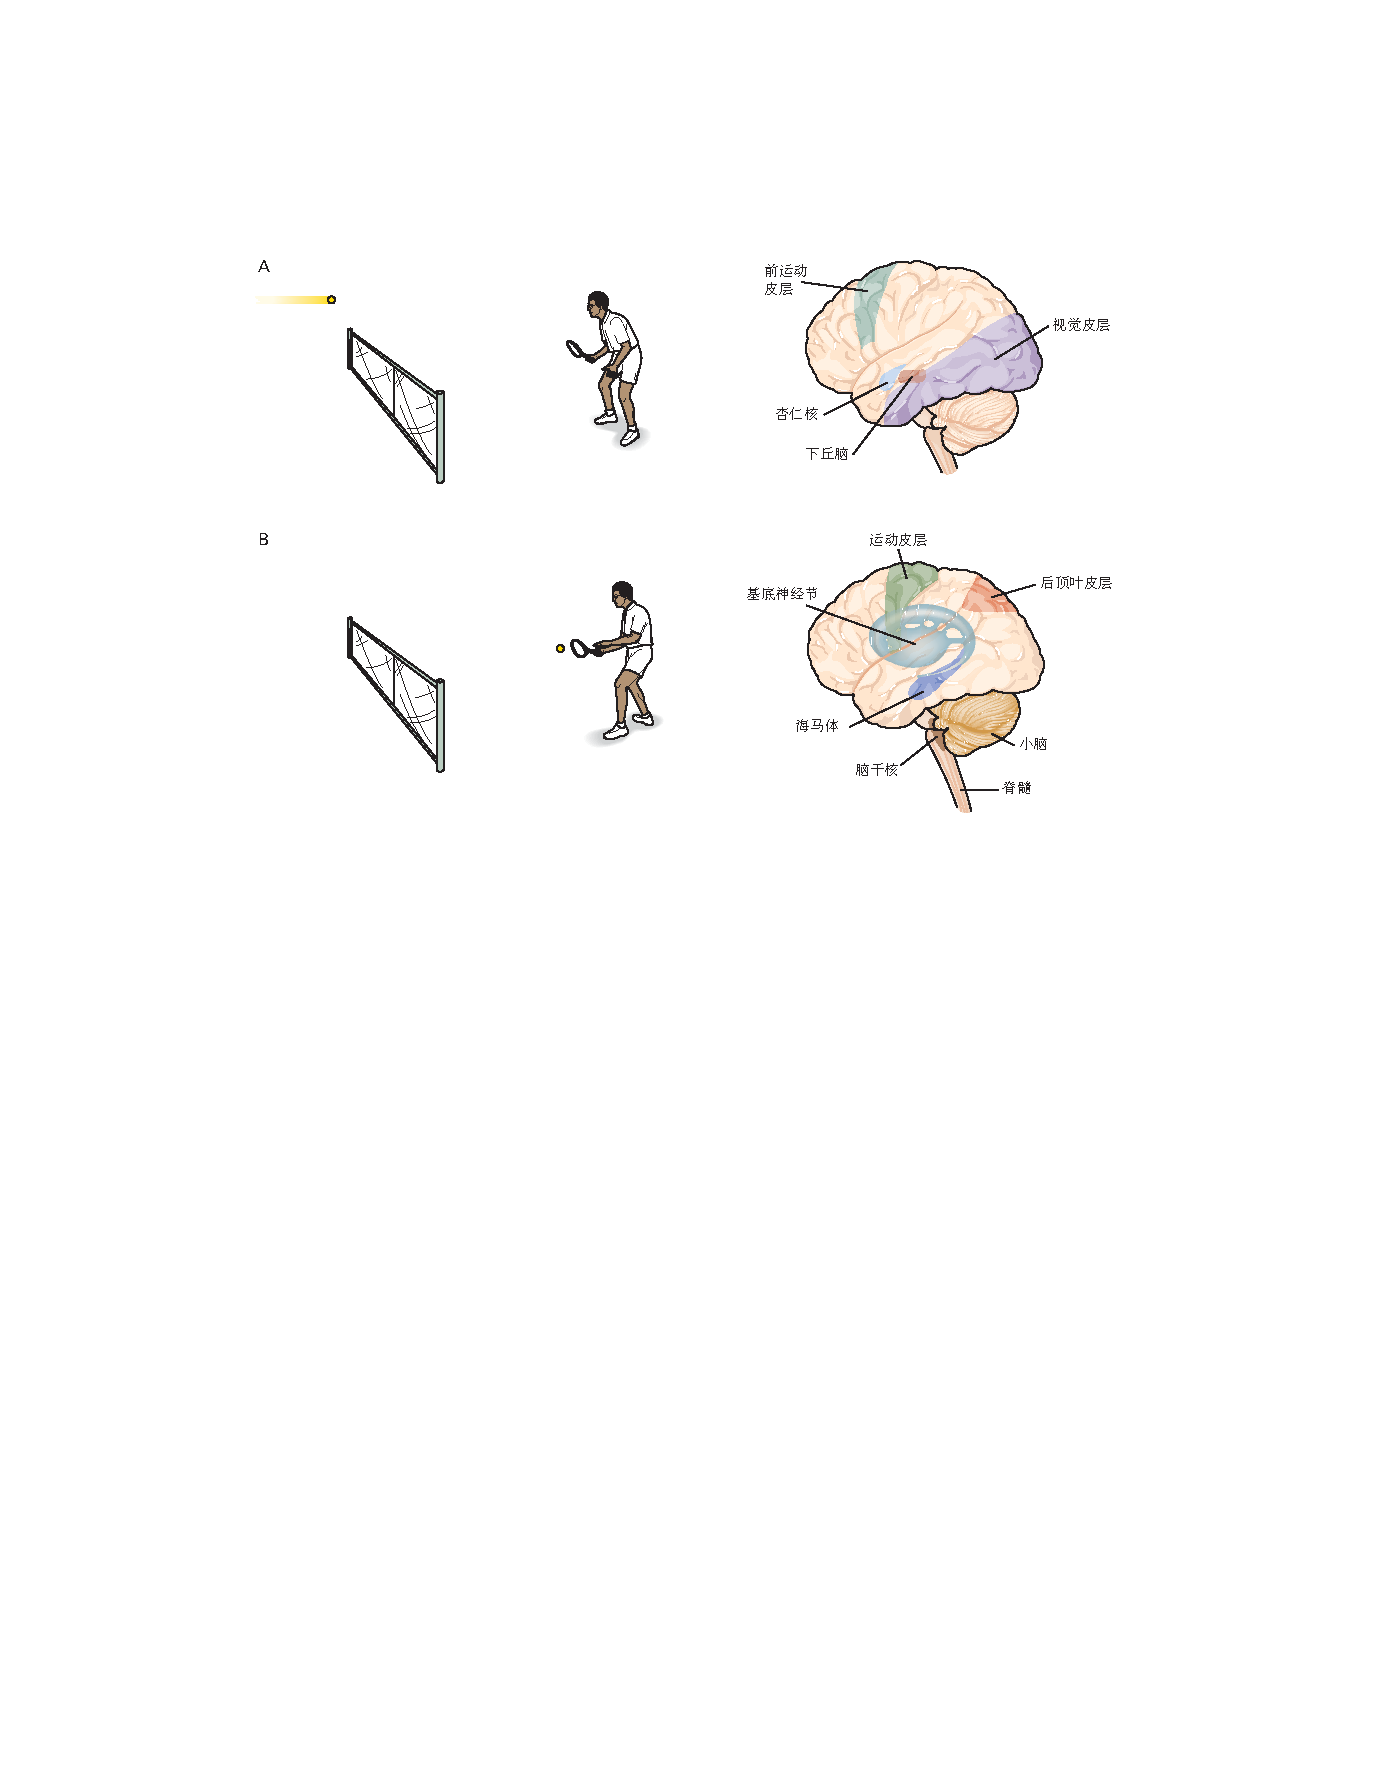
\includegraphics[width=1.0\linewidth]{chap04/fig_4_2}
	\caption{一个简单的行为是由大脑的许多部分调节的。 
		A. 一名网球运动员在观看接近的球时使用视觉皮层来判断球的大小、方向和速度。 
		前运动皮层开发了一个运动程序来回击球。 
		杏仁核与其他大脑区域协同作用,以调节心率、呼吸和其他稳态机制,并激活下丘脑以激励球员打出好球。 
		B. 为了击球,球员必须使用 A 部分中所示的所有结构以及其他结构。 
		运动皮层向脊髓发送信号,激活和抑制手臂和腿部的许多肌肉。 
		基底神经节开始参与启动运动模式,并可能回忆起学习的动作以正确击球。 
		小脑根据来自外周感觉受体的本体感受信息调整运动。 
		后顶叶皮层为球员提供了他的身体在空间中的位置以及他的球拍臂相对于他的身体的位置的感觉。 
		脑干神经元在整个运动过程中调节心率、呼吸和觉醒。 
		海马体不参与击球,而是参与存储回球的记忆,以便球员稍后可以吹嘘它。}
	\label{fig:4_2}
\end{figure}


像大多数运动行为一样,打网球并不是硬连接到大脑回路中的,而是需要学习和记忆。 
运动任务的记忆,称为程序记忆或内隐记忆,需要修改运动皮层、基底神经节和小脑中的回路。 
最后,这整个行为是可以被意识接受的,并且可以引起对过去类似经历的有意识回忆,称为外显记忆和情绪。 
外显记忆取决于海马体中的回路(第 \ref{chap:chap52} 和 \ref{chap:chap54} 章),而情绪则由杏仁核(第 \ref{chap:chap42} 和 \ref{chap:chap53} 章)和部分眶额皮质、扣带回和岛叶皮质调节。 
当然,在执行挥杆动作时,大脑也会通过同样复杂的网络协调球员的心率、呼吸和其他稳态功能。



\section{体感系统中的感官信息回路}
复杂的行为,例如区分抓球和抓书所需的运动行为,需要多个核和皮层区域的综合行动。 
信息在大脑中以分层方式处理。 
因此,有关刺激的信息通过一系列皮层下区域然后是皮层区域传递; 
在每个处理级别,信息变得越来越复杂。


此外,不同类型的信息,即使是在单一的感觉形态中,也会在几个解剖学上离散的通路中被处理。 
在体感系统中,对同一皮肤区域的轻触和针刺疼痛是由皮肤中连接到大脑中不同通路的不同感觉受体介导的。 
用于精细触觉、压力和本体感觉的系统称为表观系统,而用于疼痛和温度的系统称为原发病系统。


\subsection{来自躯干和四肢的体感信息被传送到脊髓}
来自躯干和四肢的各种形式的体感信息进入脊髓,脊髓有一个核心的 H 形灰质区域,神经元细胞体位于该区域。 
灰质被有髓轴突形成的白质包围,这些轴突构成短连接和长连接。 
脊髓两侧的灰质分为背角(或后角)和腹角(或前角)(图 \ref{fig:4_3})。

\begin{figure}[htbp]
	\centering
	\includegraphics[width=1.0\linewidth]{chap04/fig_4_3}
	\caption{脊髓的主要解剖学特征。 
		腹角(绿色)包含较大的运动神经元,而背角(橙色)包含较小的神经元。 纤
		细束的纤维携带来自下肢的体感信息,而楔形束的纤维携带来自上半身的体感信息。 
		侧柱和腹柱的纤维束包括上升和下降纤维束。}
	\label{fig:4_3}
\end{figure}


背角包含一组次级感觉神经元(感觉核),其树突从支配身体皮肤、肌肉和关节的初级感觉神经元接收刺激信息。 腹角包含运动神经元组(运动核),其轴突离开脊髓并支配骨骼肌。 
脊髓具有介导从牵张反射到肢体运动协调等行为的回路。


正如我们在第 \ref{chap:chap3} 章中讨论的那样,在考虑膝跳反射时,灰质中各种类型的中间神经元调节脊髓运动神经元的输出(见图 \ref{fig:3_5})。 
这些中间神经元中的一些是兴奋性的,而另一些是抑制性的。 
这些中间神经元调节流向大脑的感觉信息和从大脑下传至脊髓运动神经元的运动指令。 
运动神经元还可以通过中间神经元调节其他运动神经元的输出。 
当我们在第 \ref{chap:chap32} 章讨论脊髓时,将更详细地考虑这些回路。


灰质周围的白质包含成束的上升轴突和下降轴突,它们分为背侧柱、侧柱和腹侧柱。
位于灰质两个背角之间的背柱仅包含将体感信息传递到脑干的上升轴突(图 \ref{fig:4_1})。 
侧柱包括来自脑干和新皮质的上升和下降轴突,它们支配脊髓中间神经元和运动神经元(图 \ref{fig:4_3})。 
这证明了关于中枢神经系统连接的一般原则。 
处理往往是分层的:从较低到较高处理区域的投射被称为前馈,而下降投射可以调节脊髓反射并被认为是反馈。 
A 区投射到 B 区并反过来接收 B 区的返回投射的主题在整个神经系统中重复出现。 
腹侧柱还包括上升和下降轴突。 
侧柱和腹侧柱中的上升体感轴突构成平行通路,将有关疼痛和热感觉的信息传递到中枢神经系统的更高水平。 
下行轴突控制轴向肌肉和姿势。


脊髓沿其长度分为四个主要区域:颈椎、胸椎、腰椎和骶椎(图 \ref{fig:4_4})。 
从这些区域产生的连接根据肌肉、骨骼和身体其他成分发育的胚胎体节进行分离(第 45 章)。 
从脊髓突出到在同一节段发育的身体结构的轴突与在椎间孔中进入脊髓的轴突连接形成脊神经。 
颈椎水平的脊神经与头后部、颈部和手臂的感觉知觉和运动功能有关; 
胸椎神经支配上躯干; 腰椎和骶椎神经支配下躯干、背部和腿部。

\begin{figure}[htbp]
	\centering
	\includegraphics[width=1.0\linewidth]{chap04/fig_4_4}
	\caption{脊髓的内部和外部外观在不同的水平上有所不同。 
		骶骨水平的灰质(脊髓内的 H 形区域)与白质的比例大于颈椎水平。 
		在骶骨水平,很少有传入的感觉轴突与脊髓相连,而大多数运动轴突已经终止于脊髓的更高水平。 
		腰椎和颈椎水平的横截面增大是支配四肢的大量纤维进入或离开脊髓的区域。}
	\label{fig:4_4}
\end{figure}


脊髓的四个区域中的每一个区域都包含多个节段,这些节段大致对应于每个区域中的不同椎骨; 有8个颈段,12个胸段,5个腰段,5个骶段。 
成熟脊髓的实际物质看起来并不分段,但四个脊柱区域的分段仍然由进入或离开脊髓的背根和腹根的数量和位置来定义。 
由于两个组织特征,脊髓沿其 rostrocaudal 轴的大小和形状各不相同。


首先,相对较少的感觉轴突进入骶骨水平的脊髓。 进入脊髓的感觉轴突的数量在逐渐升高的水平(腰椎、胸椎和颈椎)上增加。 
相反,大多数来自大脑的下行轴突终止于颈椎水平,逐渐减少到脊髓的较低水平。 
因此,白质中的纤维数量在颈椎水平最高(上行和下行纤维数量最多),而在骶骨水平最低。 
因此,脊髓骶骨层的白质比灰质少得多,而颈髓的白质多于灰质(图 \ref{fig:4_4})。


第二个组织特征是腹角和背角大小的差异。 
腹角在运动神经支配手臂和腿部的水平较大。 
专用于身体区域的腹侧运动神经元的数量大致与该区域运动的灵巧性平行。 
因此,与躯干相比,需要更多的运动神经元来支配更多的肌肉并调节四肢更复杂的运动。 
同样,背角较大,四肢的感觉神经进入脊髓。 
四肢具有更高密度的感觉感受器来介导更精细的触觉辨别,从而将更多的感觉纤维发送到脐带。 
脊髓的这些区域被称为腰骶和颈椎增大(图 \ref{fig:4_4})。


\subsection{躯干和四肢的初级感觉神经元聚集在背根神经节}
将信息从四肢和躯干的皮肤、肌肉和关节传递到脊髓的感觉神经元聚集在脊柱内的背根神经节中,紧邻脊髓(图 \ref{fig:4_5})。 
这些神经元的形状是伪单极的; 它们有一个带有中央和外围分支的分叉轴突。 
周围分支作为游离神经末梢支配皮肤、肌肉或其他组织,或与用于感知触觉、本体感觉(拉伸感受器)、疼痛和温度的专门感受器相关联。

\begin{figure}[htbp]
	\centering
	\includegraphics[width=0.5\linewidth]{chap04/fig_4_5}
	\caption{背根神经节和脊神经根。 
		从皮肤、肌肉和关节获取感觉信息的神经元细胞体位于背根神经节,即与脊髓相邻的细胞簇。 
		这些神经元的轴突分为外围和中央分支。 
		中央分支进入脊髓的背侧部分。}
	\label{fig:4_5}
\end{figure}


体感系统及其从感受器到知觉的通路在第 \ref{chap:chap17} 章到第 \ref{chap:chap20} 章中有更全面的描述。
在这一点上,基本上有两条来自外围的体感通路,它们要么携带触摸和拉伸(epicritic 系统),要么携带疼痛和 温度(原病系统)。 
Epicritic 纤维在后柱-内侧丘系系统中移动(图 \ref{fig:4_6})。 
来自背根神经节神经元的中央定向轴突在背(或后)柱白质中上升并终止于髓质的薄核或楔形核。 
疼痛和温度通路的中枢轴突形成脊髓丘脑通路。 
它们终止于脊髓背角的灰质内。 
二级神经元穿过脊髓的另一侧并在脊髓丘脑前束和侧束中上升(图 \ref{fig:4_6})。 
两条通路最终都终止于丘脑,丘脑将投射发送到大脑皮层的初级体感区域。 
在下一节中,我们将重点关注史诗批评系统。

\begin{figure}[htbp]
	\centering
	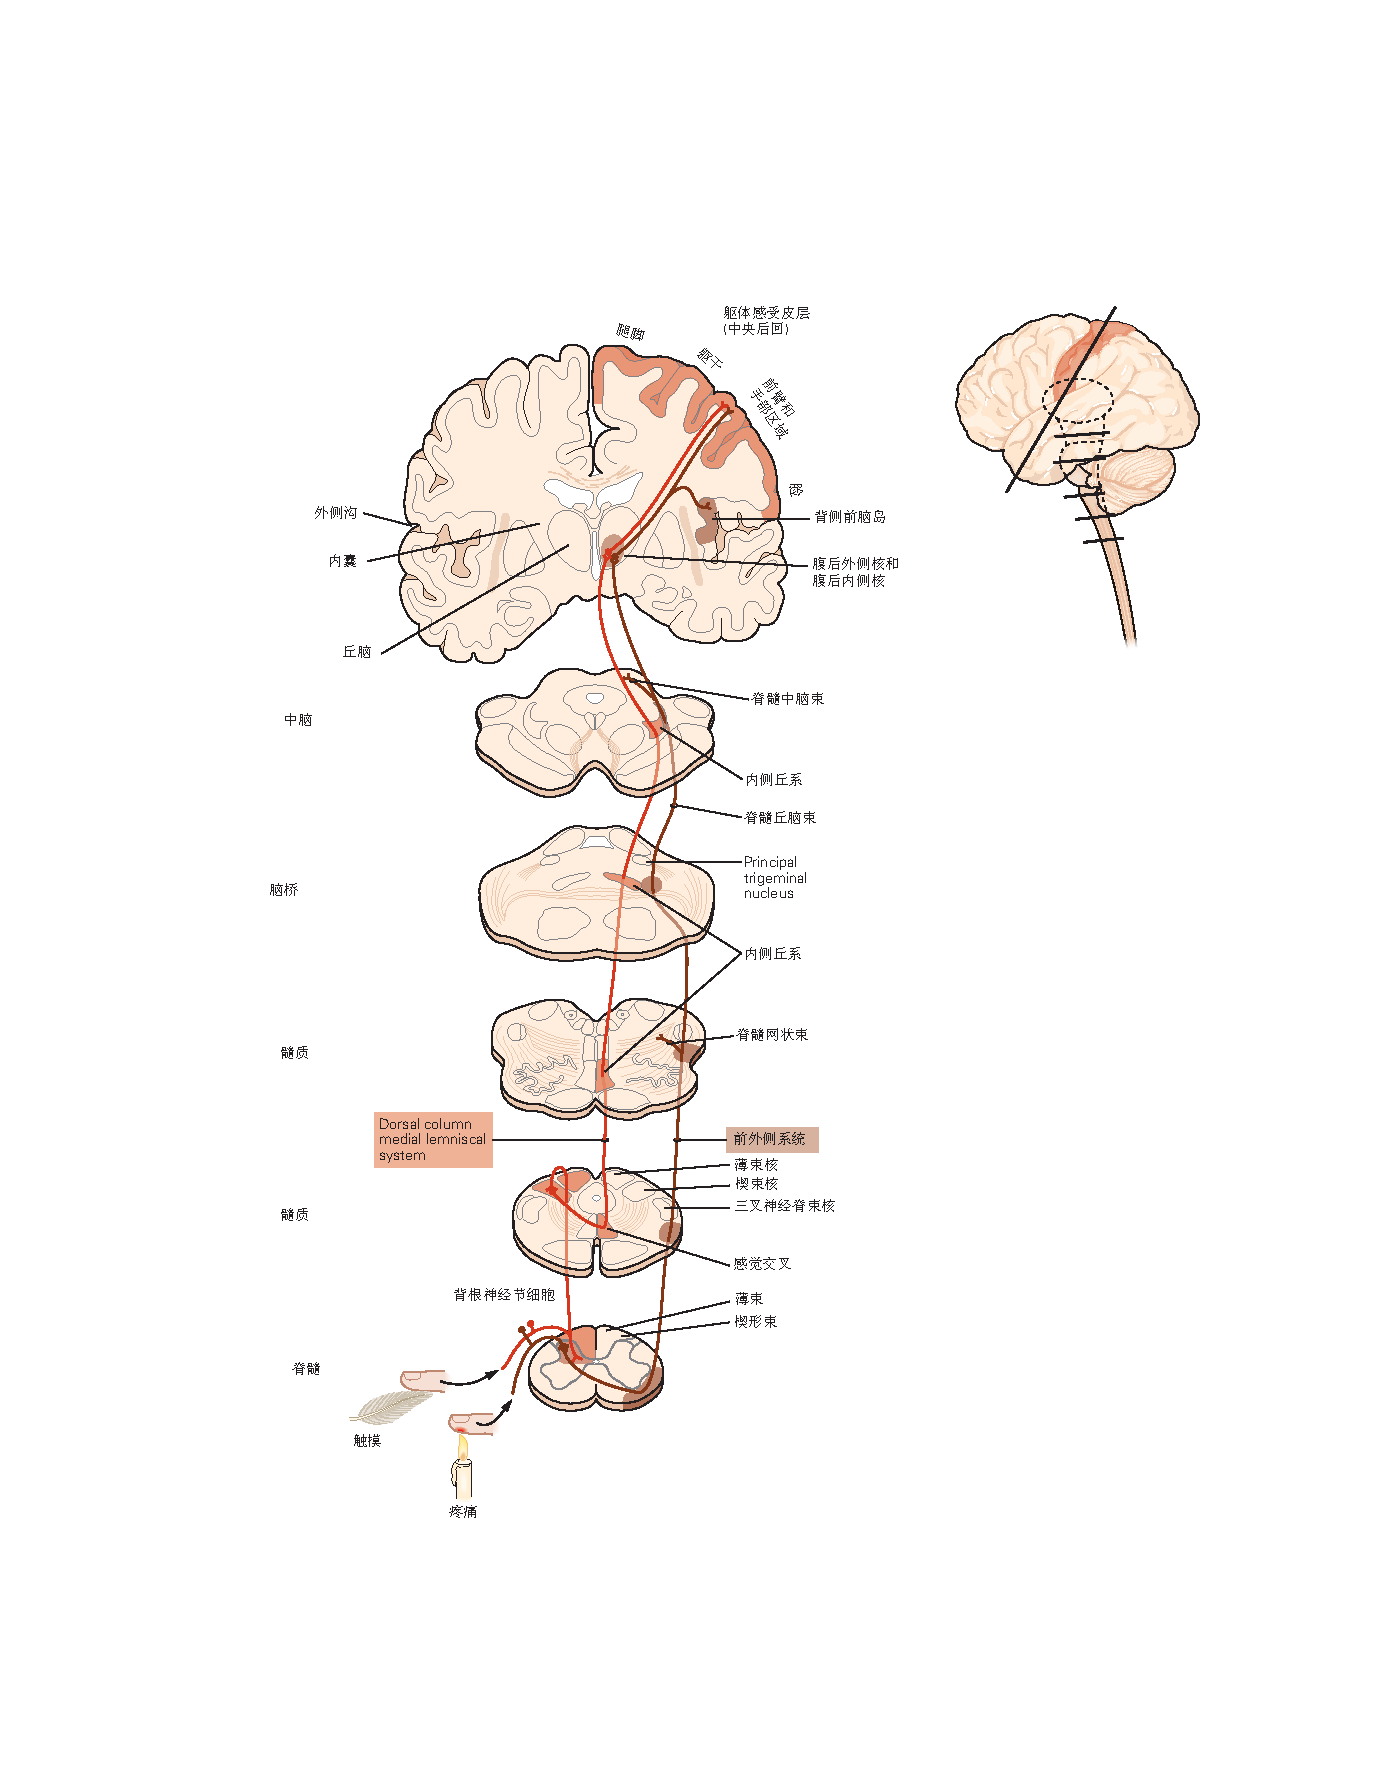
\includegraphics[width=1.0\linewidth]{chap04/fig_4_6}
	\caption{(相反)来自四肢和躯干的体感信息通过两条上行通路传递到丘脑和大脑皮层。 
		沿着从脊髓到大脑的神经轴的脑切片说明了将体感信息传递到大脑皮层的两条主要通路的解剖结构。 
		这两条通路在到达脑桥之前是分开的,它们在那里并列。 背柱-内侧丘系系统(橙色)。 
		触摸和肢体本体感觉信号通过大直径有髓神经纤维传递到脊髓和脑干,并在该系统中传递到丘脑。 
		在脊髓中,用于触觉和本体感觉的纤维分开,一个分支进入同侧脊髓灰质,另一个在同侧背柱中上升到髓质。 
		来自背柱核神经元的二级纤维在髓质中穿过中线并在对侧内侧丘系中上升至丘脑,在那里它们终止于外侧和内侧腹侧后核。 
		这些核中的丘脑神经元将触觉和本体感受信息传递给初级体感皮层。 
		前外侧系统(棕色)。 
		疼痛、瘙痒、温度和内脏信息通过终止于同侧背角的小直径有髓和无髓纤维传递到脊髓。 
		该信息由脊髓内的神经元通过中线传递,并传递到对侧前外侧系统中的脑干和丘脑。 
		终止于脑干的前外侧纤维组成脊髓网状束和脊髓中脑束; 剩余的前外侧纤维形成脊髓丘脑束。}
	\label{fig:4_6}
\end{figure}


来自触觉和本体感觉神经元的局部和上升分支为体感信息从背根神经节细胞进入脊髓提供了两条功能途径。 
局部分支可以激活调节运动输出的局部反射回路,而上行分支将信息传送到大脑,这些信息在丘脑和大脑皮层中进一步处理。


\subsection{脊髓中背根神经节神经元的中央轴突末端产生体表图}
背根神经节细胞的中央轴突终止于脊髓的方式形成了体表的神经图谱。 
来自身体表面不同部分的输入的这种有序的躯体分布在整个上升的体感通路中保持不变。 
这种排列说明了神经组织的另一个重要原则。 
在任何特定水平上构成神经回路的神经元通常以系统的方式连接并且在个体之间看起来相似。 
同样,连接神经系统不同层次不同处理区域的纤维束也以高度组织化和刻板的方式排列。


进入骶骨区脊髓的轴突在靠近中线的背柱中上升,而那些依次进入更高水平的轴突在背柱内逐渐向外侧位置上升。 
因此,在颈髓中,来自身体所有部分的轴突已经进入,来自下半身的感觉纤维位于背柱的内侧,而来自躯干、手臂和肩部,最后是颈部的纤维逐渐占据更多 横向区域。 
在颈脊髓中,形成背柱的轴突分为两束:位于内侧的纤细束和位于更外侧的楔形束(图 \ref{fig:4_1})。


\subsection{每个躯体亚模态都在从外围到大脑的不同子系统中处理}

躯体感觉的子模态——触觉、痛觉、温度觉和位置觉——在大脑中通过终止于不同大脑区域的不同通路进行处理。 
我们通过触摸子模态的信息路径来说明这些平行路径的特殊性。


携带触觉信息的初级传入纤维进入同侧背柱并上升到髓质。 
来自下半身的纤维在细束中运行并终止于细核,而来自上半身的纤维在楔形束中运行并终止于楔形核。 
纤细核和楔形核中的神经元产生轴突,轴突穿过大脑的另一侧并在称为内侧丘系的长纤维束中上升到丘脑(图 \ref{fig:4_1})。


与脊髓的背柱一样,内侧丘系的纤维按体表排列。 因为携带感觉信息的纤维穿过中线到达大脑的另一侧,大脑的右侧接收来自身体左侧的感觉信息,反之亦然。 
内侧丘系的纤维终止于丘脑的特定部分,称为腹侧后外侧核(图 \ref{fig:4_1})。 
在那里,纤维保持它们的躯体组织,使得那些从下半身传递信息的纤维在横向结束,而那些从上半身传递信息的纤维在中间终止。


\section{丘脑是感觉受体和大脑皮层之间的重要纽带}

丘脑是一个蛋形结构,构成间脑的背侧部分。 
它包含一类称为丘脑中继细胞的兴奋性神经元,可将感觉输入传递到大脑皮层的初级感觉区域。 
然而,丘脑不仅仅是一个中继站。 
它充当信息到大脑皮层的守门人,根据生物体的行为状态阻止或增强特定信息的通过。


大脑皮层的反馈投射部分终止于丘脑的一个特殊部分,称为丘脑网状核。 
这个细胞核在丘脑周围形成一层薄片,几乎完全由突触到中继细胞上的抑制性神经元组成。 
它根本不投射到新皮质。 
除了接收来自新皮质的反馈投射外,网状核还接收来自轴突的输入,离开丘脑前往新皮质,使丘脑能够调节其中继细胞对传入的感觉信息的反应。


丘脑是一个很好的例子,大脑区域由几个明确定义的核组成。 已识别出多达 50 个丘脑核团(图 \ref{fig:4_7})。 
一些细胞核接收特定于感觉方式的信息并投射到新皮层的特定区域。 
例如,腹侧后外侧核(内侧丘系终止处)中的细胞处理体感信息,它们的轴突投射到初级体感皮层(图 \ref{fig:4_1} 和 \ref{fig:4_7})。 
来自视网膜神经节细胞的投射终止于丘脑的另一部分,称为外侧膝状体核(图 \ref{fig:4_7})。 
该核中的神经元依次投射到视觉皮层。 
丘脑的其他部分参与运动功能,将信息从小脑和基底神经节传递到额叶的运动区域。 
来自投射到新皮层的丘脑细胞的轴突在辐射冠中行进,辐射冠是携带大部分轴突进出大脑半球的大纤维束。 
通过与额叶和海马体的联系,丘脑可能在记忆等认知功能中发挥作用。 
一些可能在注意力投射中起作用的核弥漫性地投射到皮层的大但明显不同的区域。


\begin{figure}[htbp]
	\centering
	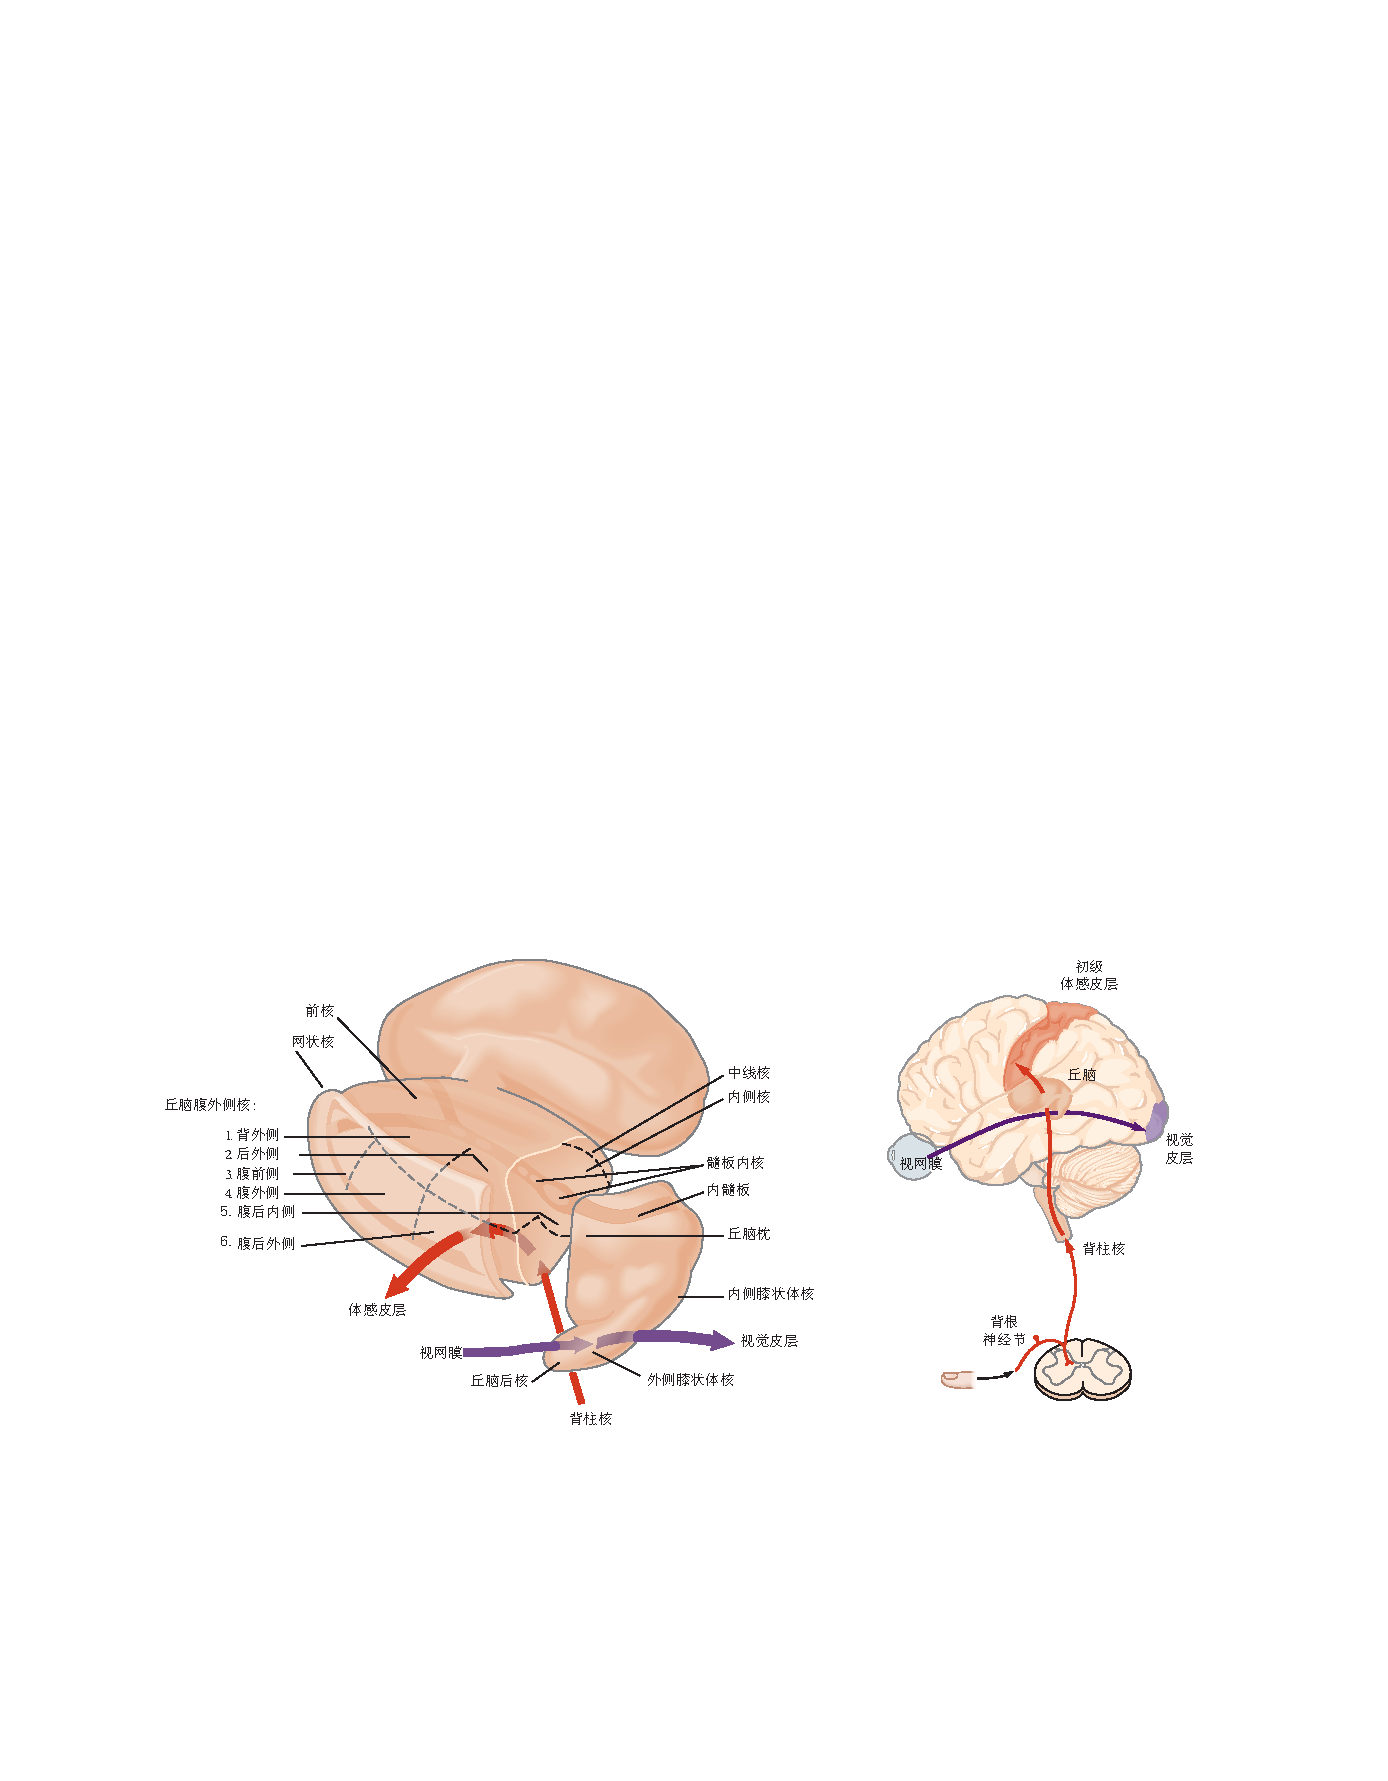
\includegraphics[width=1.0\linewidth]{chap04/fig_4_7}
	\caption{丘脑的主要部分。 
		丘脑是感觉信息从外周受体流向新皮质的关键中继站。 
		体感信息从背根神经节传递到腹侧后外侧核,然后从那里传递到初级体感皮层。 
		同样,来自视网膜的视觉信息到达外侧膝状体核,从那里传递到枕叶的初级视觉皮层。 
		除嗅觉外,每个感觉系统在丘脑的不同区域内都有类似的处理步骤。}
	\label{fig:4_7}
\end{figure}


丘脑的细胞核最常见的分为四组——前部、内侧、腹外侧和后部——相对于内髓板,一种片状纤维束,贯穿丘脑的尾部长度(图 \ref{fig:4_7}) )。
因此,内侧核团位于髓内板的内侧,而腹外侧核和后核核位于其外侧。 
在丘脑的喙极,内髓板分裂并包围前部。 
丘脑的尾极被后组占据,以枕核为主。 
神经元组也位于内髓板的纤维内,统称为板内核。


前组从下丘脑的乳头状核和海马结构的前下托接收其主要输入。 
前组的作用尚不确定,但由于其联系,被认为与记忆和情感有关。 
前组主要与扣带回和额叶皮质区域相互连接。


内侧组主要由内侧核组成。 
这个大的丘脑核分为三个部分,每个部分都与额叶皮层的特定部分相连。 
细胞核接收来自基底神经节、杏仁核和中脑部分的输入,并与记忆和情绪处理有关。


腹外侧核的命名是根据它们在丘脑内的位置命名的。 
腹侧前核和腹侧核对运动控制很重要,并将信息从基底神经节和小脑传递到运动皮层。 
腹侧后核将体感信息传递给新皮质。 
如前所述,腹后外侧核传递来自脊髓束的信息。 
腹后内侧核传递来自面部的信息,主要通过三叉神经(颅神经V)进入脑干。


后组包括内侧和外侧膝状体核、外侧后核和枕核。 
内侧膝状体是听觉系统的一个组成部分,根据其输入携带的声音频率信息按音调组织; 它将听觉信息传递到颞叶颞上回的初级听觉皮层。 
外侧膝状体接收来自视网膜的信息并将其传送到枕叶的初级视觉皮层。 
与啮齿类动物相比,灵长类大脑中的枕骨不成比例地扩大,尤其是在人类大脑中,其发育似乎与顶叶、枕叶和颞叶皮质联合区域的扩大平行。 
它已被分为至少三个分支,并与顶叶、颞叶和枕叶的广泛区域以及与视觉相关的脑干的上丘和其他核团广泛互连。


如前所述,丘脑不仅投射到新皮质(前馈连接),而且还接收来自新皮质的大量返回输入(反馈连接)。 
例如,在外侧膝状核中,轴突从视觉皮层的反馈投射形成的突触数量实际上比外侧膝状核从视网膜接收到的突触数量还要多! 
这种反馈被认为在感觉信息的处理中起着重要的调节作用,尽管确切的功能尚不清楚。 
尽管这种反馈主要来自双眼激活的皮层神经元,但外侧膝状体核中的神经元仅对一只或另一只眼睛有反应。 
这意味着它们主要是由来自视网膜(来自不同层的不同眼睛)的输入驱动的,而不是来自皮质的反馈,尽管它在数量上有优势。 
丘脑的大多数核团从大脑皮层接收到类似显着的返回投射,这些投射的意义是神经科学未解之谜之一。


到目前为止描述的丘脑核团被称为中继(或特定)核团,因为它们与新皮质的特定部分具有特定和选择性的关系。 其他丘脑核团,称为非特异性核团,投射到几个皮质和皮质下区域。 
这些核位于丘脑的中线(中线核)或内髓层内(板内核)。 
最大的中线核是室旁核、脑旁核和 reuniens 核; 最大的层内细胞群是中央核。 
椎板内核投射到内侧颞叶结构,如杏仁核和海马体,但也投射到部分基底神经节。 
这些核从脊髓、脑干和小脑中的各种来源接收输入,并被认为可以调节皮质觉醒。


丘脑是感觉处理层次结构中的重要一步,而不是将信息简单地传递到新皮质的被动中继站。 
它是一个复杂的大脑区域,在这里进行大量信息处理(图 \ref{fig:4_1})。 
仅举一个例子,来自腹侧后外侧核的体感信息的输出受到四种类型的处理:
(1)核内的局部处理;
(2) 脑干输入的调节,例如来自去甲肾上腺素能和血清素能系统; 
(3) 来自网状核的抑制性输入; 
(4) 来自新皮层的调节反馈。


\section{感觉信息处理在大脑皮层达到顶峰}

来自腹侧后外侧核的体感信息主要传递到初级体感皮层(图 \ref{fig:4_1})。 
这里的神经元对皮肤表面的触觉刺激非常敏感。 
与触觉感觉处理的早期阶段一样,体感皮层是按体位组织的(图 \ref{fig:4_8})。

\begin{figure}[htbp]
	\centering
	\includegraphics[width=1.0\linewidth]{chap04/fig_4_8}
	\caption{Homunculi 说明了专门用于身体各个部位的感觉和运动神经支配的皮质区域的相对数量。 
		整个身体表面以皮层中有序的体感输入阵列表示。 
		(摘自 Penfield 和 Rasmussen,1950 年。经麦吉尔大学 Osler 医学史图书馆许可转载。) 
		A. 专门处理身体特定部位感觉信息的皮质区域与身体的质量不成比例 身体部位,而是反映该部位感觉感受器的密度。 
		因此,来自嘴唇和手的感觉输入比来自肘部的感觉输入占据更多的皮质区域。 
		B. 运动皮层的输出以类似的方式组织。 
		专用于身体某个部位的皮质表面的数量与该部位的运动控制程度有关。 
		因此,在人类中,大部分运动皮层专用于控制手指肌肉和与语言相关的肌肉。}
	\label{fig:4_8}
\end{figure}


当神经外科医生 Wilder Penfield 在 20 世纪 40 年代末和 50 年代初刺激接受脑部手术的患者的体感皮层表面时,他发现来自下肢的感觉是由位于大脑中线附近的神经元介导的,而来自上肢的感觉 身体、手和手指、脸、嘴唇和舌头由位于侧面的神经元介导。 
Penfield 发现,虽然身体的所有部分都在皮质体表中表示,但用于每个身体部位的皮质表面积与其质量不成正比。 
相反,它与身体部位的辨别精细度成正比,而这又与感觉纤维的神经分布密度有关(第 \ref{chap:chap19} 章)。 
因此,专用于手指的皮质区域比手臂的皮质区域大。 
同样,嘴唇和舌头的表征比面部其余部分占据更多的皮质表面(图 \ref{fig:4_8})。 
正如我们将在第 \ref{chap:chap53} 章中看到的那样,用于特定身体部位的皮层数量不是固定的,而是可以根据经验进行修改,就像在音乐会小提琴手身上看到的那样,用于手指的体感皮层区域有所扩展 用来拨弦的手。 
这说明了大脑回路的一个重要方面:它能够响应使用或停用而发生可塑性变化。 
这些变化对于各种形式的学习都很重要,包括中风后恢复功能的能力。


最靠近大脑表面的大脑皮层区域被组织成层和列,这种排列提高了计算效率。 
皮质在进化过程中经历了戏剧性的扩张。 
最近的新皮质包括哺乳动物的大部分皮质。 
在较大的灵长类动物和鲸类动物的大脑中,新皮质表面是一张折叠起来有很深皱纹的薄片,因此可以将三倍多的皮质表面装入一个适度扩大的头部。 
事实上,大约三分之二的新皮质沿着皮质的深层皱纹,称为脑沟。 
新皮质的其余部分位于薄片的外部褶皱处,称为脑回。 
新皮质接收来自丘脑、大脑两侧的其他皮质区域和其他皮质下结构的输入。 
它的输出被定向到皮质、基底神经节、丘脑、桥脑核和脊髓的其他区域。


这些复杂的输入-输出关系在皮质神经元的有序分层中得到有效组织; 每层包含不同的输入和输出。 
新皮质的许多区域,特别是初级感觉区域,包含六层,从大脑外表面到白质编号(图 \ref{fig:4_9})。

\begin{figure}[htbp]
	\centering
	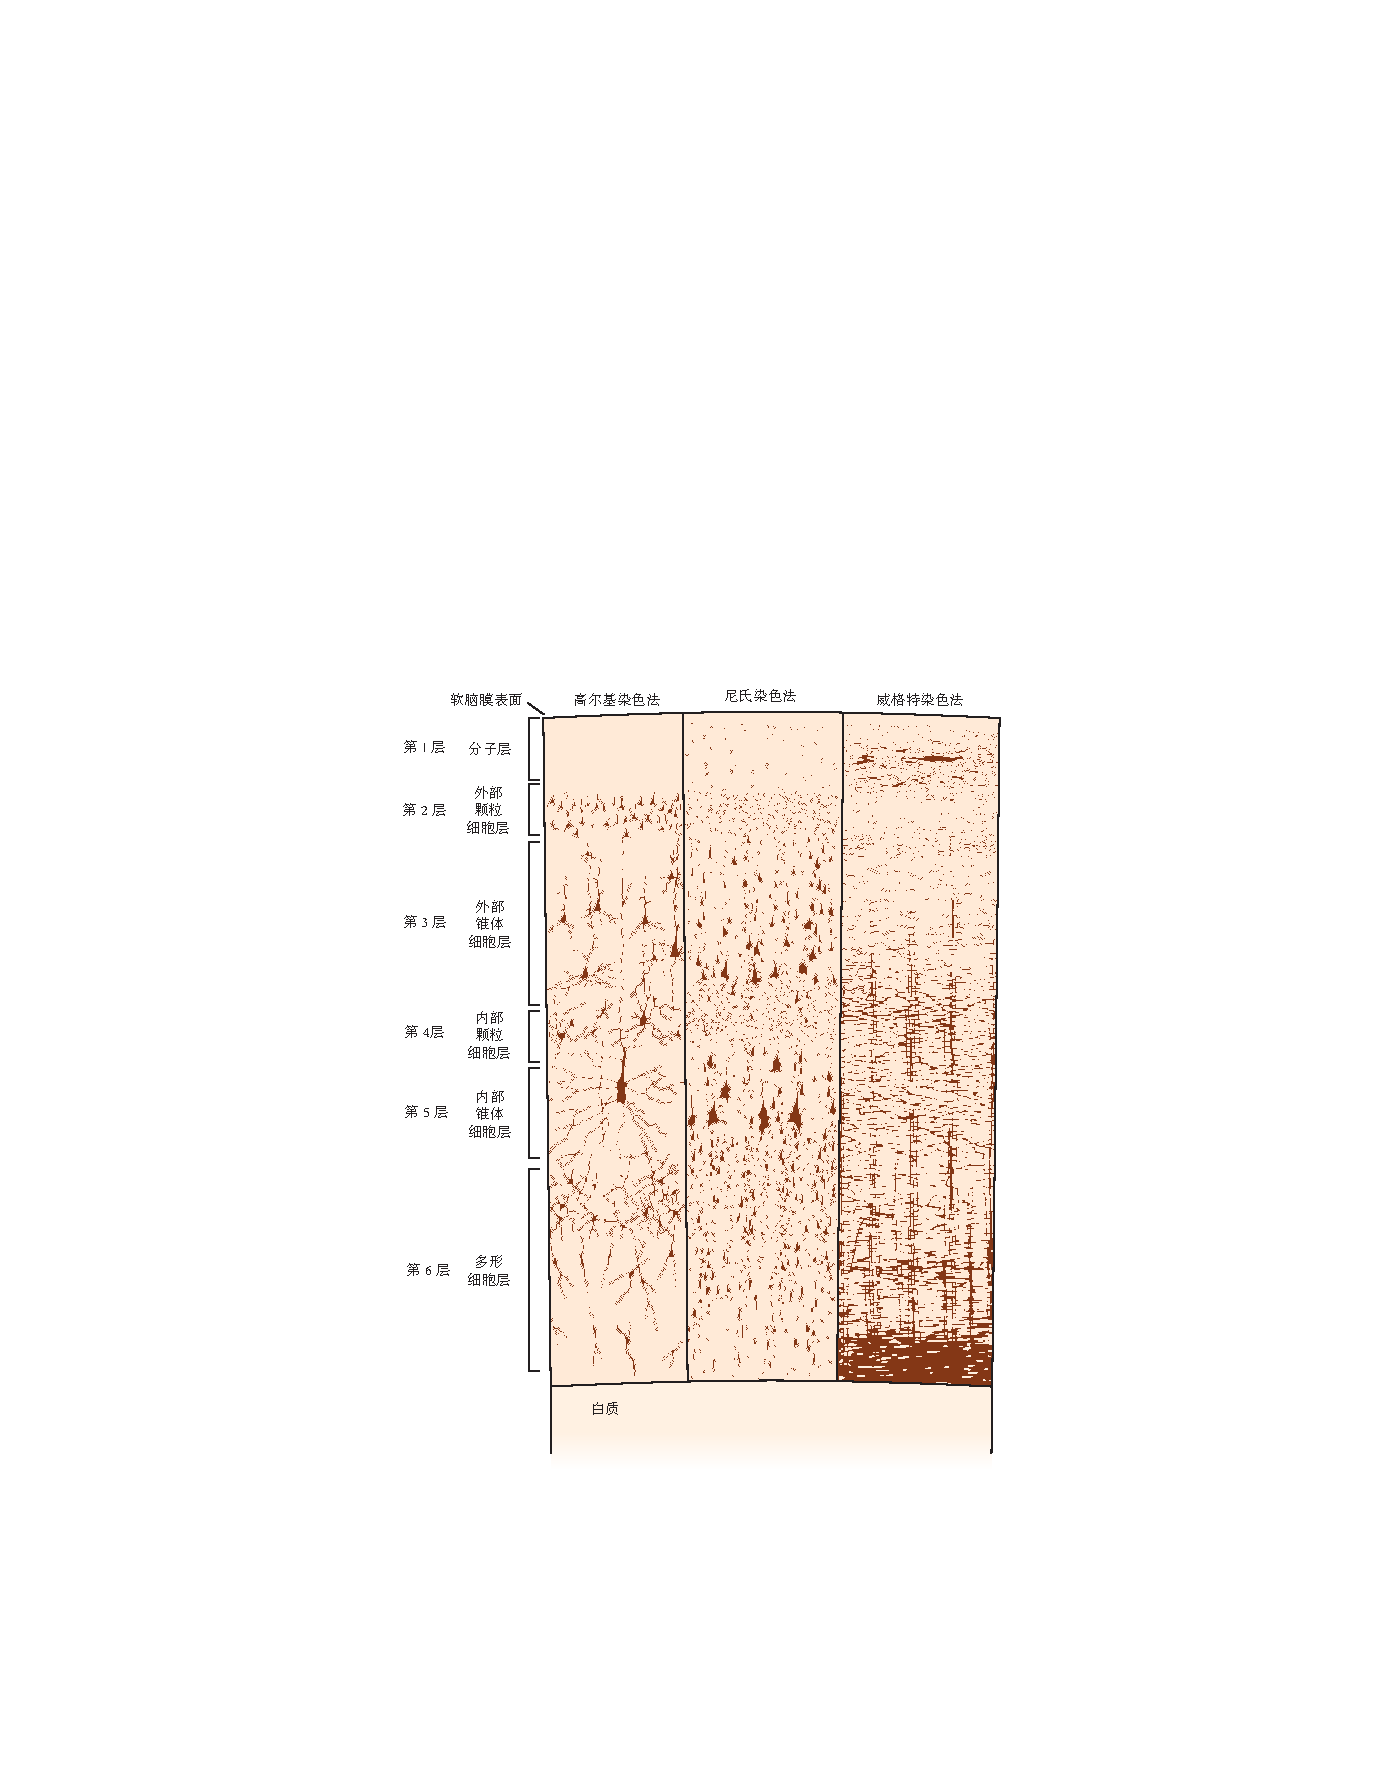
\includegraphics[width=1.0\linewidth]{chap04/fig_4_9}
	\caption{新皮质的神经元排列成不同的层次。 
		新皮质的外观取决于用来染色的物质。 
		高尔基体染色(左)揭示了神经元细胞体、轴突和树突树的一个子集。 
		Nissl 方法(中)显示细胞体和近端树突。 
		Weigert 染色(右)揭示了有髓纤维的模式。 (经许可转载自 Heimer 1994。)}
	\label{fig:4_9}
\end{figure}


第一层,即分子层,由位于更深层的细胞的树突和穿过该层以在皮层的其他区域建立连接的轴突占据。


第二层和第三层主要包含小的金字塔形细胞。 
第二层,外部颗粒细胞层,是包含小球形神经元的两层之一。 
第三层称为外锥体细胞层(内锥体细胞层位于更深的水平)。 
位于第三层较深的神经元通常比位于较浅层的神经元大。 
II 层和 III 层锥体神经元的轴突局部投射到同一皮质区域内的其他神经元以及其他皮质区域,从而调节皮质内通讯(图 \ref{fig:4_10})。

\begin{figure}[htbp]
	\centering
	\includegraphics[width=1.0\linewidth]{chap04/fig_4_10}
	\caption{新皮质不同层的神经元投射到大脑的不同部分。 
		对新皮层所有其他部分的投射,即所谓的皮质或联合连接,主要来自第 II 层和第 III 层的神经元。 
		对皮层下区域的投射主要来自第五层和第六层。 (经许可转载自 Jones 1986。)}
	\label{fig:4_10}
\end{figure}


第四层包含大量小球形神经元,因此称为内部颗粒细胞层。 
它是丘脑感觉输入的主要接受者,在初级感觉区最为突出。 
例如,作为初级视觉皮层的枕叶皮层区域有一个非常突出的第四层。 
该区域的第 IV 层由神经元组成,非常复杂,通常分为三个子层。 
具有突出的第 IV 层的区域称为颗粒状皮层。 
相比之下,初级运动皮层所在的中央前回基本上没有第四层,因此是所谓的无颗粒额叶皮层的一部分。 
这两个皮质区域是组织学切片中最容易识别的区域之一(图 \ref{fig:4_11})。

\begin{figure}[htbp]
	\centering
	\includegraphics[width=1.0\linewidth]{chap04/fig_4_11}
	\caption{新皮层每个细胞层的范围在整个皮层各不相同。 
		皮层的感觉区域,例如初级视觉皮层,往往有一个非常突出的内部颗粒细胞层(第 IV 层),即感觉输入的位置。 
		皮层的运动区域,例如初级运动皮层,有一个非常微薄的第 IV 层,但有突出的输出层,例如第 V 层。
		这些差异导致 Korbinian Brodmann 和其他人在 20 世纪之交将皮层分为各种细胞结构 地区。 
		这里展示的布罗德曼 1909 年的细分是经典分析,但基于单个人脑。 (经许可转载自 Martin 2012。)}
	\label{fig:4_11}
\end{figure}


第 V 层,即内部锥体细胞层,主要包含金字塔形细胞,这些细胞通常比第 III 层中的细胞大。 
该层中的锥体神经元产生皮质的主要输出通路,投射到其他皮质区域和皮质下结构(图 \ref{fig:4_9})。


VI 层中的神经元在形状上相当异质,因此这一层称为多态层或多形式层。 
它融入形成皮层深层界限的白质中,并携带轴突进出皮层区域。


各个层的厚度及其功能组织的细节在整个皮质中各不相同。 
大脑皮层的早期研究者 Korbinian Brodmann 使用第 IV 层上下各层的相对突出程度、细胞大小和包装特征来区分新皮层的不同区域。 
基于这种细胞结构差异,1909 年,Brodmann 将大脑皮层分为 47 个区域(图 \ref{fig:4_11})。


尽管 Brodmann 的分界部分与新皮层局部功能的信息一致,但细胞构造方法本身并不能捕捉到皮层所有不同区域功能的微妙之处或多样性。 
例如,Brodmann 确定了五个区域(区域 17-21)与猴子的视觉功能有关。 
相比之下,现代连接神经解剖学和电生理学已经在 Brodmann 识别的五个区域中识别出超过 35 个功能不同的皮层区域。


在新皮质内,信息通过前馈和反馈连接从一个突触中继传递到另一个突触中继。 
例如,在视觉系统中,从初级视觉皮层到二级和三级视觉区域的前馈投射主要起源于第三层,主要终止于目标皮层区域的第四层。 
相反,对早期处理阶段的反馈投射源自第 V 层和第 VI 层的细胞,并终止于第 I、II 和 VI 层(图 \ref{fig:4_12})。

\begin{figure}[htbp]
	\centering
	\includegraphics[width=1.0\linewidth]{chap04/fig_4_12}
	\caption{上升和下降皮层通路的区别在于它们在皮层层内的起源和终止的组织。 
		上行或前馈通路通常起源于皮层的表层,并总是终止于第 IV 层。 
		下行或反馈路径通常起源于深层并终止于第一层和第六层。 (经许可改编自 Felleman 和 Van Essen 1991。)}
	\label{fig:4_12}
\end{figure}


大脑皮层在功能上被组织成从白质延伸到皮层表面的细胞柱。 
(这种柱状组织在标准组织学制备中并不特别明显,最初是在电生理学研究中发现的。)每根柱状物的直径约为三分之一毫米。 
每列中的单元格形成一个具有高度专业化功能的计算模块。 
列内的神经元往往具有非常相似的响应特性,大概是因为它们形成了局部处理网络。 
专用于某个功能的皮质区域越大,专用于该功能的计算列的数量就越多(第 \ref{chap:chap23} 章)。 
手指具有高度辨别力的触觉是大面积皮层中许多专门处理来自手的体感信息的皮层柱的结果。


除了皮层柱的识别之外,早期电生理学研究的第二个主要见解是体感皮层包含的不是一个而是几个身体表面的体表图。 
初级躯体感觉皮层(前顶叶皮层)有四张完整的皮肤图,布罗德曼区 3a、3b、1 和 2 各一张。丘脑并行发送大量深层受体信息(例如,来自肌肉) 区域 3a 和它的大部分皮肤信息到区域 3b 和 1。
区域 2 接收来自这些丘脑皮质区域的输入,并且可能负责我们对三维立体物体的综合感知,称为立体视觉。 
初级体感皮层中的神经元投射到邻近区域的神经元,而这些神经元又投射到其他邻近的皮层区域(图\ref{fig:4_13})。 
在皮层连接层次结构的更高层次上,体感信息用于运动控制、手眼协调和与触觉相关的记忆。

\begin{figure}[htbp]
	\centering
	\includegraphics[width=1.0\linewidth]{chap04/fig_4_13}
	\caption{大脑皮层中感觉信息的处理从初级感觉区开始,在单峰关联区继续,并在多峰关联区进一步阐述。 
		感觉系统还与运动皮层的部分进行通信。 例如,初级体感皮层投射到额叶的运动区和顶叶皮层的体感联合区。 
		反过来,体感关联区投射到高阶体感关联区和运动前皮层。 
		来自不同感觉系统的信息汇聚在多模式关联区域,其中包括海马旁、时间关联和扣带皮层。}
	\label{fig:4_13}
\end{figure}


参与感觉处理早期阶段的皮层区域主要与单一感觉方式有关。 这些区域称为初级感觉或单峰(感觉)关联区域。 
来自单峰关联区域的信息会聚在与组合感觉方式有关的皮层多峰关联区域(图 \ref{fig:4_13})。 
这些与海马体密切相关的多模态关联区域似乎对两个功能特别重要:
(1) 统一知觉的产生和 
(2) 知觉在记忆中的表征(我们将在后面讨论这个问题) 本章结束)。


因此,从皮肤感受器上的机械压力到手指被握手的朋友触摸的感知,体感信息在从背根神经节到大脑的一系列越来越复杂的回路(网络)中进行处理。 
体感皮层,到单峰关联区,最后到多峰关联区。 
体感信息的主要目的之一是指导定向运动。 
正如人们想象的那样,皮层的体感和运动功能之间存在着密切的联系。

\section{自主运动是由皮层和脊髓之间的直接连接介导的}

正如我们将在第 \ref{chap:chap25} 章和第 \ref{chap:chap30} 章中看到的那样,知觉系统的一个主要功能是为运动系统调节的动作提供必要的感觉信息。 
初级运动皮层的组织结构类似于体感皮层(图 \ref{fig:4_8}B)。 
运动皮层的特定区域影响特定肌肉群的活动(第 \ref{chap:chap34} 章)。


初级运动皮层 V 层神经元的轴突提供新皮层的主要输出以控制运动。 
一些 V 层神经元通过皮质脊髓束中投射到脊髓腹角中的运动神经元直接影响运动。 
其他人通过突触到髓质中的运动输出核或基底神经节中的纹状体神经元上来影响运动控制。 
人类皮质脊髓束由大约一百万个轴突组成,其中大约 40\% 起源于运动皮层。 
这些轴突向下穿过皮层下白质、内囊和中脑的大脑脚(图 \ref{fig:4_14})。 
在髓质中,纤维在腹面形成突出的突起,称为髓质金字塔,因此整个突起有时称为锥体束。

\begin{figure}[htbp]
	\centering
	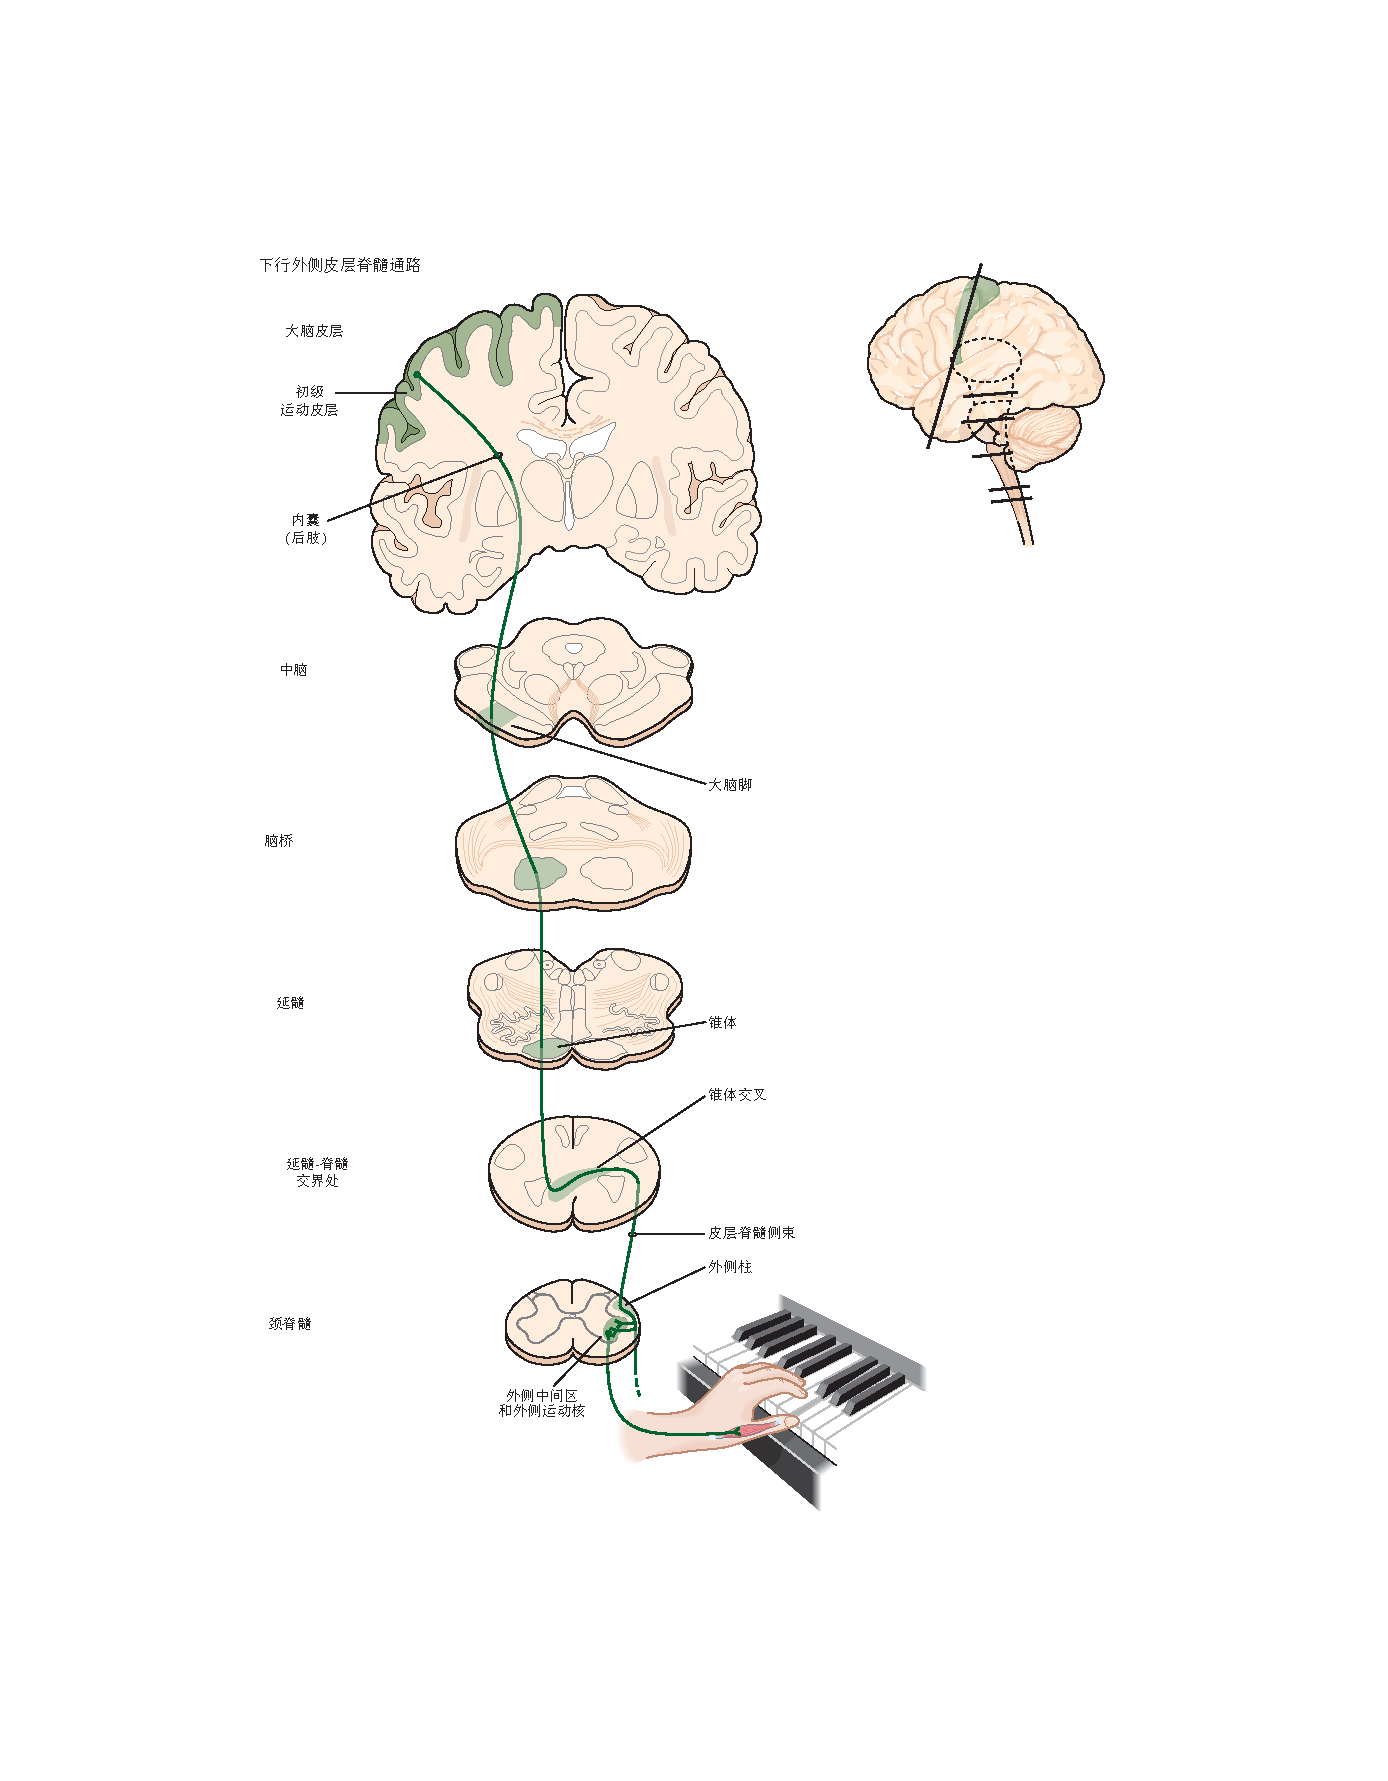
\includegraphics[width=1.0\linewidth]{chap04/fig_4_14}
	\caption{皮质脊髓束中的大量纤维起源于初级运动皮层并终止于脊髓的腹角。
		相同的轴突在其投射的不同点处是内囊、大脑脚、髓质金字塔和外侧皮质脊髓束的一部分。}
	\label{fig:4_14}
\end{figure}


与上行体感系统一样,下行皮质脊髓束穿过脊髓的另一侧。 
大多数皮质脊髓纤维在称为锥体交叉的位置穿过髓质中线。 
然而,大约 10\% 的纤维在到达它们将终止的脊髓水平之前不会交叉。 
皮质脊髓纤维与运动神经元建立单突触连接,这种连接对于个性化的手指运动尤为重要。 
它们还与脊髓中的兴奋性和抑制性中间神经元形成突触,这些连接对于在伸手和行走等行为中协调较大的肌肉群很重要。


皮质脊髓束中携带的运动信息受到感觉信息和来自其他运动区域的信息的显着调节。 
需要连续不断的触觉、视觉和本体感受信息流,才能使随意运动既准确又顺序正确。 
此外,运动皮层的输出受到大脑其他运动区域的重大影响,包括小脑和基底神经节,这些结构对于顺利执行运动至关重要。 
这两个皮层下区域在第 \ref{chap:chap37} 章和第 \ref{chap:chap38} 章中有详细描述,它们提供对熟练动作的顺利执行必不可少的反馈,因此对于通过练习提高运动技能也很重要(图 \ref{fig:4_15} )。

\begin{figure}[htbp]
	\centering
	\includegraphics[width=1.0\linewidth]{chap04/fig_4_15}
	\caption{自主运动需要协调电机系统的所有组件。 
		主要成分是运动皮层、基底神经节、丘脑、中脑、小脑和脊髓。 
		主要下降投影以绿色显示; 反馈预测和本地连接以紫色显示。 
		所有这些处理都包含在脊髓腹角运动神经元的输入中,即所谓的“最终共同通路”,它支配肌肉并引发运动。 
		(这张图是从不同角度拍摄的大脑部分的合成视图。)}
	\label{fig:4_15}
\end{figure}


\section{大脑中的调节系统影响动机、情绪和记忆}
大脑的某些区域既不是纯粹的感觉也不是纯粹的运动,而是调节特定的感觉或运动功能。 
调节系统通常涉及对饥饿、口渴或睡眠等基本需求做出反应的行为。 
例如,下丘脑中的感觉和调节系统决定血糖水平(第 \ref{chap:chap41} 章)。 
当血糖降至某个临界水平以下时,我们就会感到饥饿。 
为了满足饥饿感,大脑中的调节系统将视觉、听觉和嗅觉集中在与进食相关的刺激上。


脑干内不同的调节系统调节注意力和觉醒(第 \ref{chap:chap40} 章)。 
脑干中的小核含有合成和释放调节性神经递质去甲肾上腺素(蓝斑)和血清素(中缝背核)的神经元。 
这些神经元通过与前脑结构的广泛联系来设定动物的一般觉醒水平。 
一组胆碱能调节神经元,即 Meynert 基底核,参与觉醒或注意力(第 \ref{chap:chap40} 章)。 
该核位于端脑基底前脑部分的基底神经节下方。 
其神经元的轴突基本上投射到新皮质的所有部分。


如果捕食者发现潜在的猎物,各种皮层和皮层下系统将决定猎物是否可食用。 
一旦识别出食物,其他皮层和皮层下系统就会启动一个全面的自愿运动程序,使动物与猎物接触、捕获猎物并将其放入口中、咀嚼和吞咽。


最后,动物在进食中的生理满足感强化了导致成功捕食的行为。 
中脑中的一组多巴胺能神经元对于监测强化和奖励很重要。 
多巴胺能调节系统的力量已经通过实验证明,在实验中,将电极植入大鼠的奖励区域,让动物自由地按下杠杆以电刺激它们的大脑。 
他们更喜欢这种自我刺激,而不是获取食物或水、进行性行为或任何其他自然有益的活动。 
第 \ref{chap:chap38} 章描述了多巴胺能调节系统在通过强化探索行为进行学习中的作用。


与奖励、注意力和动机有关的大脑调节系统如何与感觉和运动系统相互作用是神经科学中最有趣的问题之一,也是我们理解学习和记忆存储的基础(第 \ref{chap:chap40} 章)。


\section{周围神经系统在解剖学上与中枢神经系统不同}
周围神经系统为中枢神经系统提供有关身体外部环境和内部环境的连续信息流。 
它具有躯体和自主神经分裂(图 \ref{fig:4_16} )。

\begin{figure}[htbp]
	\centering
	\includegraphics[width=0.5\linewidth]{chap04/fig_4_16}
	\caption{周围神经系统具有躯体神经和自主神经分裂。 
		躯体分裂将信息从皮肤传递到大脑,再从大脑传递到肌肉。 
		自主神经系统调节非自愿功能,包括心脏活动以及肠道和腺体中的平滑肌。}
	\label{fig:4_16}
\end{figure}


躯体分裂包括从皮肤、肌肉和关节接收信息的感觉神经元。 
这些感觉神经元的细胞体位于背根神经节和颅神经节中。 与这些细胞相关的受体提供有关肌肉和肢体位置以及体表触摸和压力的信息。 
在第四部分(感知)中,我们将看到这些感受器在将一种或另一种物理能量(例如深压力或热量)转换为神经系统使用的电信号方面是多么的专业化。 
在第五部分(运动)中,我们将看到肌肉和关节中的感觉感受器对于塑造身体的连贯运动至关重要。


周围神经系统的自主神经分裂介导内脏感觉以及内脏、血管系统和外分泌腺的运动控制。 
它由交感神经系统、副交感神经系统和肠道系统组成。 
交感神经系统参与身体对压力的反应,而副交感神经系统则起到保护身体资源和恢复体内平衡的作用。 
肠神经系统,神经元细胞体位于或邻近内脏,控制平滑肌和肠道分泌物的功能。 
第 \ref{chap:chap41} 章描述了自主神经系统的功能组织,第 \ref{chap:chap42} 章描述了它在情绪和动机中的作用。


\section{记忆是一种复杂的行为,由不同于执行感觉或运动的结构介导}
过去 50 年的研究提供了大脑中记忆系统的复杂视图。 
我们现在知道不同形式的记忆(例如,恐惧记忆与技能记忆)由不同的大脑区域调节。 
在这里,我们对比了负责编码和存储我们对其他个人、地点、事实和事件的体验的系统组织,这个过程称为外显记忆。


我们知道称为海马体的结构(或更准确地说是海马体结构,因为它包含多个皮层区域)是编码和存储我们生活记忆的内侧颞叶记忆系统的关键组成部分(图 \ref{fig:4_17})。 
这种理解主要基于对著名患者亨利·莫莱森(Henry Molaison,生前研究过他的科学家简称为 HM)的分析,他在 1950 年代初进行了双侧颞叶手术以减轻危及生命的癫痫症。 
与六层新皮质相比,海马体连同嗅觉皮质(梨状皮质)是一种三层皮质结构,称为原皮质,是系统发育较早的皮质区域之一。

\begin{figure}[htbp]
	\centering
	\includegraphics[width=1.0\linewidth]{chap04/fig_4_17}
	\caption{用 Nissl 方法染色的人海马体形成的冠状切片,以展示细胞体。 
		主要的细胞构造场显示在人类海马结构的这一部分中。 
		(缩写:CA3 和 CA1,海马体的细分;DG,齿状回;EC,内嗅皮质;F,菌毛;Sub,下托。)}
	\label{fig:4_17}
\end{figure}

我们在本章中简要描述海马结构的原因是要强调并非所有大脑回路都是相似的。 
事实上,无论是谈论嗅觉开始处理的嗅球,还是细化精细运动的小脑,一般原则是回路的结构特定于它所调节的功能。
海马体回路与人们想象的调节感官知觉或运动运动的回路截然不同。 
大脑的海马体回路将在后面的章节中更详细地讨论。 
第 \ref{chap:chap5} 章介绍了海马体对动物在其环境中的空间位置信息进行编码以及外显记忆(包括空间记忆)的编码需要突触功能发生可塑性变化的观点。 
第 \ref{chap:chap52} 章和第 \ref{chap:chap54} 章分别探讨了人类记忆功能以及外显记忆和空间表征的细胞和分子基础。

\subsection{海马系统与最高级别的多感觉皮层区域相互连接}

感觉系统是分层的,并且在更高层次上逐渐处理更复杂的刺激,特别是新皮质。 
此外,从每个模态的最高级别,电路连接位于皮层周围不同位置的多感觉皮层区域,来自许多感觉模态的信息会聚到单个神经元上。 
海马体系统从几个特定的多感觉区域接收大部分输入,即制造记忆的原材料。 
这些包括位于内侧颞叶的鼻周和海马旁皮质,以及位于扣带回尾部的脾后皮质。 
这些多感觉区域汇聚在海马系统的入口结构上,即内嗅皮层(图 \ref{fig:4_18})。 
进入内嗅皮层的多感觉信息可以被认为是对即时经验的总结。

\begin{figure}[htbp]
	\centering
	\includegraphics[width=1.0\linewidth]{chap04/fig_4_18}
	\caption{与海马结构连接的层次组织。 
		海马结构主要通过内嗅皮层从多模态关联区域(例如鼻周、海马旁和脾后皮质)接收高度处理的感觉信息。}
	\label{fig:4_18}
\end{figure}

\subsection{海马结构由几个不同但高度集成的电路组成}
海马结构由许多不同的皮质区域组成,这些区域的组织比新皮质更简单——至少它们的层数更少。 
这些区域包括齿状回、海马体、下托和内嗅皮质。 
这些区域中的每一个都由包含许多神经元细胞类型的子区域组成。 
海马结构中最简单的子区域是齿状回,它有一个称为颗粒细胞的主要神经元。 
海马体的亚区域称为 CA1、CA2 和 CA3,由单层锥体细胞组成,其树突在细胞体层上方和下方延伸,并接收来自多个区域的输入。 
下托(分为下托、前托和副托)是另一个主要由锥体细胞组成的区域。 
最后,海马结构中最复杂的部分是内嗅皮质,它有多层,但仍然具有与新皮质明显不同的组织。 
例如,它缺少第 IV 层,而具有更突出的第 II 层。


\subsection{海马结构主要由单向连接组成}

在这里,我们描述了海马结构的基本电路。 
该电路在第 \ref{chap:chap54} 章中有更详细的描述。
图 \ref{fig:4_19} 中显示的海马电路的简化版本强调了它对多模式感觉信息的逐步串行处理,每个海马区域都有助于外显记忆的形成。 
这种串行处理意味着对该系统的任何一个组件的损坏都会导致记忆障碍。 
事实上,另一名姓名缩写为 R.B. 的著名患者确实因缺血发作后 CA1 区域的细胞丢失而遭受严重的记忆障碍。

\begin{figure}[htbp]
	\centering
	\includegraphics[width=0.5\linewidth]{chap04/fig_4_19}
	\caption{海马结构内部连接的简化图。 
		该回路从内嗅皮层 II 层的细胞开始到齿状回,然后投射到海马体的 CA3 区域。 
		海马体的 CA3 部分投射到 CA1,然后 CA1 投射到下托。 
		当下托突出到内嗅皮层的深层时,海马回路关闭。 
		未显示的是从内嗅皮层到它从中接收感觉信息的相同多模态区域的反馈通路。}
	\label{fig:4_19}
\end{figure}

事实证明,虽然海马体的形成对于我们生活记忆的初始形成至关重要,但这些记忆最终存储在大脑的其他地方。 
在像 HM 这样的患者中,内嗅皮质和大部分海马系统的其余部分都被切除了,手术前的记忆基本完好无损。 
因此,为了实现我们生活记忆的创造和长期储存,海马体和内嗅皮层必须与大脑皮层中的回路进行交流。 
发生这种情况的地点和具体方式仍然是个谜。


\section{亮点}

1. 单个神经元不能进行行为。 它们必须被纳入由不同类型的神经元组成的电路中,这些神经元通过兴奋性、抑制性和调节性连接相互连接。

2. 感觉和运动信息在大脑中同时活跃的各种不同的大脑区域中进行处理。

3. 功能通路由可识别的脑区串联而成,每个脑区的回路比前一个脑区处理更复杂或更具体的信息。

4. 触觉和痛觉是由脊髓、脑干、丘脑和新皮质中不同回路之间的通路介导的。 

5. 所有的感觉和运动系统都遵循分层和相互处理信息的模式,而海马体记忆系统主要是为非常复杂的多感觉信息的串行处理而组织的。 一般原则是大脑中的电路具有适合其执行功能的组织结构。 

6. 与对我们个人经历的直觉分析相反,感知并不是我们周围世界的精确复制品。 感觉是对现实的抽象,而不是复制。 在首先分析外部物理事件的各种特征之后,大脑的回路构建了外部物理事件的内部表征。 当我们把一个物体拿在手里时,不同的大脑区域会根据大脑自身的规律,同时对物体的形状、运动和质地进行分析,并将结果整合到有意识的体验中。 

7. 感觉如何整合到有意识的体验中——绑定问题——以及有意识的体验如何从大脑对传入的感觉信息的分析中浮现出来,这是认知神经科学中最有趣的两个问题(第 56 章)。 一个更复杂的问题是这些有意识的印象是如何编码成存储数十年的记忆的。

\section{选读}
\section{参考文献}
























\chapter{调节行为的神经回路的计算基础}
% PDF所在目录: /data2/whd/win10/learn/neuro/neuro_神经科学原理_28_中枢神经系统的听觉处理.pdf

\section{神经放电模式提供信息编码}

\subsection{感觉信息由神经活动编码}
\subsection{可以从神经活动中解码信息}
\subsection{可以解码海马空间认知图来推断位置}
% 定位


\section{神经回路基序为信息处理提供了基本逻辑}
\subsection{视觉处理和对象识别取决于前馈表示的层次结构}
\subsection{小脑中不同的神经元表征为学习提供了基础}
\subsection{循环回路是持续活动和整合的基础}

\section{学习和记忆取决于突触可塑性}
\subsection{突触输入的主导模式可以通过赫布可塑性来识别}
\subsection{小脑的突触可塑性在运动学习中起着关键作用}

\section{亮点}
\section{选读}
\section{参考文献}


\chapter{成像和行为}
% PDF所在目录: /data2/whd/win10/learn/neuro/neuro_神经科学原理_28_中枢神经系统的听觉处理.pdf

\section{功能性 MRI 实验测量神经血管活动}

\subsection{fMRI 取决于磁共振物理学}
\subsection{fMRI 依赖于神经血管耦合的生物学}

\section{可以通过多种方式分析功能性 MRI 数据}
\subsection{fMRI 数据首先需要通过以下预处理步骤准备分析}
\subsection{fMRI 可用于将认知功能定位到特定的大脑区域}
\subsection{fMRI 可用于解码大脑中代表的信息}
\subsection{fMRI 可用于测量大脑网络中的相关活动}

\section{功能性 MRI 研究带来了基本的见解}
\subsection{人类的 fMRI 研究启发了动物的神经生理学研究}
\subsection{fMRI 研究挑战了认知心理学和系统神经科学的理论}
\subsection{fMRI 研究检验了动物研究和计算模型的预测}

\section{功能性 MRI 研究需要仔细解读}

\section{未来的进步取决于技术和概念的进步}

\section{亮点}

\section{推荐读物}

\section{参考文献}

\chapter{神经系统的细胞}
% PDF所在目录: /data2/whd/win10/learn/neuro/neuro_神经科学原理_28_中枢神经系统的听觉处理.pdf

\section{神经元和胶质细胞具有许多结构和分子特征}

\section{细胞骨架决定细胞形状}

\section{蛋白质颗粒和细胞器沿轴突和树突主动运输}
\subsection{快速轴突运输携带膜细胞器}
\subsection{缓慢的轴突运输携带细胞溶质蛋白和细胞骨架的元素}


\section{与其他分泌细胞一样,蛋白质也是在神经元中制造的}
\subsection{分泌蛋白和膜蛋白在内质网中合成和修饰}
\subsection{分泌蛋白在高尔基复合体中被修饰}

\section{表面膜和细胞外物质在细胞内循环}

\section{胶质细胞在神经功能中发挥多种作用}
\subsection{胶质细胞形成轴突的绝缘鞘}
\subsection{星形胶质细胞支持突触信号}
\subsection{小胶质细胞在健康和疾病中具有多种功能}

\section{脉络丛和室管膜细胞产生脑脊液}

\section{亮点}

\section{选读}

\section{参考文献}

\chapter{离子通道} \label{chap:chap8}

大脑中的信号传导取决于神经细胞对非常小的刺激做出反应的能力,以及跨细胞膜的电势差的快速和大幅度变化。 
在感觉细胞中,膜电位会响应微小的物理刺激而发生变化:
眼睛中的受体对单个光子作出反应;
嗅觉神经元检测单个气味分子;
内耳中的毛细胞对原子尺寸的微小运动作出反应。
这些感觉反应最终导致动作电位的激发,在此期间膜电位以每秒 500 伏特的速度变化。


构成整个神经系统信号传导基础的膜电位的快速变化是由膜上称为离子通道的特殊孔或开口介导的,离子通道是一类存在于身体所有细胞中的整合膜蛋白。
神经细胞的离子通道经过优化调整以响应特定的物理和化学信号。
它们也是异质的——在神经系统的不同部分,不同类型的通道执行特定的信号任务。


由于它们在电信号中的关键作用,离子通道的故障会导致多种神经系统疾病(第~\ref{chap:chap57}~和~\ref{chap:chap58}~章)。
离子通道故障引起的疾病不仅限于大脑;
例如,囊性纤维化、骨骼肌疾病和某些类型的心律失常也是由离子通道功能障碍引起的。
此外,离子通道通常是药物、毒物或毒素的作用部位。
因此,离子通道在神经系统的正常生理学和病理生理学中都具有至关重要的作用。


除了离子通道,神经细胞还含有第二类重要的蛋白质,专门用于移动离子穿过细胞膜,即离子转运蛋白和泵。
这些蛋白质不参与快速神经元信号传导,但对于建立和维持细胞内外之间生理上重要离子的浓度梯度很重要。
正如我们将在本章和下一章中看到的,离子转运蛋白和离子泵在重要方面与离子通道不同,但也有某些共同特征。


离子通道具有三个重要特性:
(1)它们识别和选择特定离子;
(2) 它们响应特定的电气、化学或机械信号而打开和关闭;
(3) 它们传导离子穿过膜。
神经和肌肉中的通道以极快的速度传导离子穿过细胞膜,从而提供大量电荷。
每秒有多达 1 亿个离子可以通过一个通道。
该电流导致信号所需的膜电位快速变化(第 ~\ref{chap:chap10}~章)。
离子通过通道的快速流动与最快的酶、过氧化氢酶和碳酸酐酶的周转率相当,后者受底物扩散的限制。
(大多数其他酶的周转率要慢得多,从每秒 10 到 1,000 不等。)


尽管离子流速如此之快,但通道对它们允许渗透的离子具有惊人的选择性。
每种类型的通道仅允许一种或几种类型的离子通过。
例如,神经细胞的负静息电位主要由一类 \ce{K+} 通道决定,这些通道对 \ce{K+} 的渗透性比对 \ce{Na+} 高 100 倍。
相反,动作电位的产生涉及一类 \ce{Na+} 通道,它们对 \ce{Na+} 的渗透性比对 \ce{K+} 的渗透性高 10 到 20 倍。
因此,神经元信号转导的多功能性的关键是不同类别离子通道的调节激活,每个离子通道都对特定离子具有选择性。


许多通道响应特定事件而打开和关闭:
电压门控通道由膜电位的变化调节,配体门控通道由化学递质的结合调节,机械门控通道由膜拉伸调节。
当细胞静止时,其他通道通常是开放的。
通过这些“静止”通道的离子通量在很大程度上决定了静止电位。


离子通过离子通道的流动是被动的,不需要通道消耗代谢能量。
离子通道仅限于催化离子被动运动以降低其热力学浓度和电梯度。
这种通量的方向不是由通道本身决定的,而是由跨膜的静电和扩散驱动力决定的。
例如,\ce{Na+} 离子在动作电位期间通过电压门控 \ce{Na+} 通道流入细胞,因为外部 \ce{Na+} 浓度远大于内部浓度;
开放通道允许 \ce{Na+} 沿着浓度梯度扩散到细胞中。
通过这种被动离子运动,如果没有离子泵,\ce{Na+} 浓度梯度最终会消散。
不同类型的离子泵保持 \ce{Na+}、\ce{K+}、钙离子和其他离子的浓度梯度。


这些泵在两个重要细节上不同于离子通道。
首先,虽然开放的离子通道具有连续的充满水的通道,离子通过该通道畅通无阻地从膜的一侧流向另一侧,但每次泵移动一个离子或一组离子穿过膜时,它必须经历一系列构象变化。
因此,通过泵的离子流速度比通过通道慢 100 到 100,000 倍。
其次,维持离子梯度的泵使用化学能(通常以三磷酸腺苷 (ATP) 的形式)来逆着电梯度和化学梯度输送离子。
这种离子运动称为主动传输。
离子泵和传输器的功能和结构将在本章末尾和第 ~\ref{chap:chap9}~章中详细讨论。


在本章中,我们将研究六个问题:为什么神经细胞有通道?
通道如何以如此高的速率传导离子并且仍然具有选择性? 
通道是如何门控的?
这些通道的特性如何被各种内在和外在条件所改变?
通道结构如何解释功能?
最后,通过通道的离子运动与通过转运蛋白的离子运动有何不同?
在后续章节中,我们将考虑静息通道和泵如何产生静息电位(第~\ref{chap:chap9}~章)、电压门控通道如何产生动作电位(第~\ref{chap:chap10}~章)以及配体门控通道如何产生突触电位(第 11、12 和 13)。



\section{离子通道是跨越细胞膜的蛋白质}

要理解为什么神经细胞使用通道,我们需要了解质膜的性质和溶液中离子的物理化学性质。
所有细胞(包括神经细胞)的质膜厚度约为 6 至 8 nm,由脂质和蛋白质镶嵌而成。
膜的核心由大约 3 至 4 nm 厚的双层磷脂形成。
嵌入在这个连续的脂质片中的是完整的膜蛋白,包括离子通道。


膜的脂质不与水混合——它们是疏水的。
相反,细胞内的离子和细胞外的离子强烈吸引水分子——它们是亲水性的(图~\ref{fig:8_1})。
离子吸引水是因为水分子是偶极的:虽然水分子上的净电荷为零,但分子内的电荷是分离的。
水分子中的氧原子倾向于吸引电子,因此带有少量的净负电荷,而氢原子倾向于失去电子,因此带有少量的净正电荷。
由于这种不均匀的电荷分布,带正电的离子(阳离子)被强烈地静电吸引到水中的氧原子上,而带负电的离子(阴离子)被吸引到氢原子上。
同样,离子吸引水; 它们被静电束缚的水合水所包围(图~\ref{fig:8_1})。


\begin{figure}[htbp]
	\centering
	\includegraphics[width=0.6\linewidth]{chap08/fig_8_1}
	\caption{(相反)细胞膜对离子的渗透性取决于离子与水、膜脂双层和离子通道的相互作用。 溶液中的离子被一团水分子(水合水)包围,这些水分子被离子的净电荷吸引。 当离子在溶液中扩散时,该云被离子携带,增加了离子的有效尺寸。 离子离开这个极性环境进入由磷脂形成的脂质双层的非极性环境在能量上是不利的,因此不太可能。 磷脂具有亲水性头部和疏水性尾部。 疏水性尾巴连接在一起以排除水和离子,而极性亲水性头部则面向细胞外液和细胞质的水性环境。 磷脂由甘油主链组成,其中两个 -OH 基团通过酯键与脂肪酸分子相连。 甘油的第三个-OH基团与磷酸相连。 磷酸基团进一步连接到各种小的极性醇头基团 (R) 之一。 离子通道是跨越脂质双层的完整膜蛋白,为离子穿过膜提供了途径。 这些通道对特定离子具有选择性。 钾通道具有排除 \ce{Na+} 的窄孔。 虽然 \ce{Na+} 离子比 \ce{K+} 离子小,但在溶液中,\ce{Na+} 的有效直径更大,因为它的局部场强更强,导致它吸引更大的水分子云。 \ce{K+} 通道孔太窄,水合 \ce{Na+} 离子无法渗透。 钠通道具有选择性过滤器,可弱结合 \ce{Na+} 离子。 根据 Bertil Hille 及其同事提出的假设,\ce{Na+} 离子在穿过过滤器时会在活性位点短暂结合。 在结合位点,离子的正电荷被通道壁上带负电荷的氨基酸残基和被通道壁另一侧第二极性氨基酸残基吸引的水分子稳定。 人们认为,\ce{K+} 离子由于其直径较大,无法通过负电荷有效稳定,因此会被过滤器排除。 (改编自 Hille 1984。)}
	\label{fig:8_1}
\end{figure}


除非消耗大量能量来克服离子与周围水分子之间的吸引力,否则离子不能从水中移动到膜中脂质双层的不带电碳氢化合物尾部。
出于这个原因,离子极不可能从溶液中移动到脂质双层中,因此,双层本身几乎完全不能渗透离子。
相反,离子通过离子通道穿过膜,其中能量学有利于离子运动。


虽然只有大约 35 年的时间才确定它们的分子性质,但离子通道的概念可以追溯到 19 世纪末 Ernst Brücke 的工作。
生理学家早就知道,尽管细胞膜充当屏障,但细胞膜仍然可以渗透水和许多小溶质,包括一些离子。
为了解释渗透作用,即水在生物膜上的流动,Brücke 提出膜包含允许水流动但不允许较大溶质流动的通道或孔隙。
100 多年后,彼得·阿格雷 (Peter Agre) 发现称为水通道蛋白的蛋白质家族形成了对水具有高度选择性渗透性的通道。
在 20 世纪初,William Bayliss 提出充满水的通道可以让离子轻松穿过细胞膜,因为离子不需要从水合水中剥离。


离子通过通道移动的想法引出了一个问题:充满水的通道如何能够以高速率传导离子并且具有选择性?
例如,通道如何允许 \ce{K+} 离子通过而排除 \ce{Na+} 离子?
选择性不能仅基于离子的直径,因为晶体半径为 0.133 nm 的 \ce{K+} 大于 \ce{Na+}(晶体半径为 0.095 nm)。
决定离子选择性的一个重要因素是离子水合水壳的大小,因为离子在溶液中移动的难易程度(其迁移率)取决于离子及其周围水壳的大小。
离子越小,其电荷局域化程度越高,电场越强。
结果,较小的离子更强烈地吸引水。
因此,当 \ce{Na+} 在溶液中移动时,它对水的更强静电吸引导致它具有更大的水壳,相对于 \ce{K+} 往往会减慢它的速度。
由于其较大的水壳,\ce{Na+} 表现得好像比 \ce{K+} 大。
离子越小,其在溶液中的迁移率越低。
因此,我们可以构建一个选择 \ce{K+} 而不是 \ce{Na+} 的通道模型,仅基于充满水的通道中两种离子与水的相互作用(图~\ref{fig:8_1})。


尽管此模型解释了通道如何选择 \ce{K+} 并排除 \ce{Na+},但并未解释通道如何选择 \ce{Na+} 并排除 \ce{K+}。
这个问题导致 1930 年代和 40 年代的许多生理学家放弃了通道理论,转而支持离子通过首先与特定载体蛋白结合而穿过细胞膜的想法,然后载体蛋白将离子穿梭穿过细胞膜。
在这种载体模型中,选择性基于离子和载体蛋白之间的化学结合,而不是离子在溶液中的迁移率。


尽管我们现在知道离子可以通过各种运输大分子穿过膜,\ce{Na+}-\ce{K+} 泵是一个典型的例子(第~\ref{chap:chap9}~章),但膜离子渗透性的许多特性并不符合载体模型。
最重要的是离子跨膜转移的速度很快。 
当神经递质乙酰胆碱 (ACh) 与其在神经-肌肉突触的突触后膜中的受体结合时,跨膜电流就提供了一个例子。
如后所述,单个 ACh 受体传导的电流为每秒 1250 万个离子。
相比之下,\ce{Na+}-\ce{K+} 泵每秒最多传输 100 个离子。


如果 ACh 受体充当载体,它必须在 0.1 微秒(百万分之一秒)内将离子穿梭穿过膜,这是一个令人难以置信的速度。
\ce{Na+}-\ce{K+} 泵和 ACh 受体之间 100,000 倍的速率差异强烈表明 ACh 受体(和其他配体门控受体)必须通过通道传导离子。
后来在许多对 \ce{K+}、\ce{Na+} 和钙离子具有选择性的电压门控通路中进行的测量也证明了单个大分子携带的大电流,表明它们也是通道。

但我们仍然面临什么使渠道具有选择性的问题。
为了解释选择性,Bertil Hille 扩展了孔隙理论,提出通道具有充当分子筛的狭窄区域。
在这个选择性过滤器中,离子必须排出大部分水合水才能穿过通道;
取而代之的是弱化学键(静电相互作用)与排列在通道壁上的极性(带电)氨基酸残基形成(图~\ref{fig:8_1})。
因为排出水合水在能量上是不利的,所以只有当离子与选择性过滤器相互作用的能量补偿了与其水合水相互作用的能量损失时,离子才会穿过通道。
穿过通道的离子通常仅在短时间内(小于 1 μs)与选择性过滤器结合,之后静电和扩散力推动离子穿过通道。
在孔径大到足以容纳几个水分子的通道中,离子不需要完全脱离其水壳层。


这种化学识别和特异性是如何建立的?
George Eisenman 在 1960 年代早期提出了一种理论来解释离子选择性玻璃电极的特性。
根据这一理论,具有高负场强的结合位点——例如,由带负电荷的谷氨酸或天冬氨酸羧酸基团形成的位点——将比 \ce{K+} 更紧密地结合 \ce{Na+}。
这种选择性的产生是因为两个带电基团之间的静电相互作用受库仑定律约束,与两个基团之间的距离成反比。


因为它的晶体半径比 \ce{K+} 小,所以 \ce{Na+} 可以比 \ce{K+} 更接近具有高负场强的结合位点,因此会在结合时产生更有利的自由能变化。
这补偿了 \ce{Na+} 失去一些水合水以穿过窄选择性过滤器的要求。
相比之下,具有低负场强的结合位点(例如,由极性羰基或羟基氧原子组成的结合位点)会选择 \ce{K+} 而不是 \ce{Na+}。
在这样的位置,\ce{Na+} 的结合不会提供足够的自由能变化来补偿离子的水合水的损失,而 \ce{Na+} 具有很强的水合水。
然而,由于较大的 \ce{K+} 离子与水的相互作用较弱,因此这样的位点将能够补偿 \ce{K+} 离子水合水的损失。
目前认为离子通道是选择性的,因为这种特定的化学相互作用和基于孔径的分子筛分。



\section{所有细胞中的离子通道都有几个功能特征}

大多数细胞都能够发出局部信号,但只有神经和肌肉细胞专门用于长距离快速信号传递。
尽管神经和肌肉细胞具有特别丰富的种类和高密度的膜离子通道,但它们的通道与体内其他细胞的通道没有根本区别。
在这里,我们描述了各种细胞中离子通道的一般特性,这些细胞是通过在各种实验条件下记录流过通道的电流来确定的。



\subsection{可以记录通过单个离子通道的电流}

离子通道的研究最初仅限于记录通过一类离子通道的整个群体的总电流,这种方法掩盖了通道功能的一些细节。
后来的发展使得通过单个离子通道记录电流获得更高的分辨率成为可能。
Erwin Neher 和 Bert Sakmann 于 1976 年首次直接记录了生物膜中的单个离子通道。
将含有 ACh(激活骨骼肌膜中 ACh 受体的神经递质)的玻璃微量移液器紧紧压在肌肉膜上。
从移液器尖端下方的膜记录代表单个 ACh 受体通道打开和关闭的小单一电流脉冲。
当前脉冲都具有相同的幅度,表明通道以全有或全无的方式打开(方框~\ref{box:8_1})。


\begin{proposition}[单离子通道中的电流记录:膜片钳] \label{box:8_1}
	
	\quad \quad 膜片钳技术是由Erwin Neher和Bert Sakmann于1976年开发的,用于记录单离子通道的电流。
	它是对原始电压箝位技术的改进(见方框10-1)。
	
	\quad \quad 将一个尖端直径约为1μm的小型火抛光玻璃微量移液管压在骨骼肌纤维膜上。
	与微量移液管中电解质接触的金属电极将移液管连接到一个特殊的电路上,该电路测量通过移液管尖端下膜通道的电流(图~\ref{fig:8_2}A)。
	
	\quad \quad 1980年,Neher发现,对贴片移液管进行少量抽吸可以大大提高移液管和膜之间的密封性。
	结果是在移液管的内部和外部之间具有极高阻力的密封。
	该密封降低了电子噪声,并将膜片钳技术的实用性扩展到整个离子通道范围。
	自这一发现以来,膜片钳技术已被用于研究各种神经元和其他细胞中的所有主要类型的离子通道(图~\ref{fig:8_2}B)。
	
	\quad \quad 克里斯托弗·米勒(ChristopherMiller)独立开发了一种将离子通道从生物膜整合到人工脂质双层中的方法。
	他首先在搅拌器中将膜均质化;
	然后,通过离心匀浆,他分离出仅由膜囊泡组成的部分。
	他使用保罗·米勒(PaulMueller)和唐纳德·鲁丁(DonaldRudin)在20世纪60年代开发的技术研究了这些囊泡的功能成分。
	他们发现了如何通过在分离两种盐溶液的非导电屏障上的孔上画一薄层磷脂来创建人工脂质双层。
	米勒发现,在适当的离子条件下,他的膜囊泡与平面磷脂膜融合,将囊泡中的任何离子通道结合到平面膜中。
	
	\quad \quad 这种技术有两个实验优势。
	首先,它允许从膜片钳无法接近的细胞区域的离子通道进行记录;
	例如,米勒成功地研究了从骨骼肌内膜(肌浆网)分离的\ce{K+}通道。
	其次,它使研究人员能够研究膜脂质的组成如何影响通道功能。
	
\end{proposition}


\begin{figure}[htbp]
	\centering
	\includegraphics[width=0.8\linewidth]{chap08/fig_8_2}
	\caption{膜片钳设置和记录。
	\textbf{A.} 在盐水溶液中含有低浓度乙酰胆碱(ACh)的移液管用于记录通过骨骼肌ACh受体通道的电流。(改编自Alberts等人,1994年。)
	\textbf{B.} 当通道在闭合状态和打开状态之间切换时,膜片钳记录通过单个ACh受体通道的电流。(经许可转载自B.Sakmann。)}
	\label{fig:8_2}
\end{figure}



在 –80 mV 的膜电位下测得的脉冲为 2 pA (2 × 10–12 A),根据欧姆定律 (I = V/R) 表明通道的电阻为 5 × 1011 欧姆。
在处理离子通道时,谈论电导更有用,即电阻的倒数 (γ = 1/R),因为它提供了与离子渗透性相关的电测量。
因此,单个离子通道的欧姆定律可表示为 i = γ × V。ACh 受体通道的电导约为 25 × 10–12 西门子 (S),或 25 皮西门子 (pS),其中 1 S 等于 1 /欧姆。



\subsection{通过通道的离子通量不同于自由溶液中的扩散}

离子渗透的动力学特性最好用通道的电导来描述,通道的电导是通过测量响应电化学驱动力通过开放通道的电流(离子通量)来确定的。
净电化学驱动力由两个因素决定:
跨膜的电势差和跨膜的渗透离子的浓度梯度。
改变其中任何一个都可以改变净驱动力(第~\ref{chap:chap9}~章)。


在一些开放通道中,电流随驱动力线性变化——也就是说,通道表现为简单的电阻器。
在其他情况下,电流是驱动力的非线性函数。
这种类型的通道起到整流器的作用——由于通道结构或离子环境的不对称性,它在一个方向上比在另一个方向上更容易传导离子(图~\ref{fig:8_3})。


\begin{figure}[htbp]
	\centering
	\includegraphics[width=1.0\linewidth]{chap08/fig_8_3}
	\caption{电流-电压关系。 在许多离子通道中,通过开放通道的电流 (i) 与膜电压 (Vm) 之间的关系是线性的(左图)。 此类通道被称为“欧姆”通道,因为它们遵循欧姆定律,i = Vm /R 或 Vm × γ,其中 γ 是电导。 在其他通道中,电流和膜电位之间的关系是非线性的。 这种通道被称为“整流”,因为它比另一个方向更容易在一个方向上传导电流。 右图显示了一个外向整流通道,对于给定的电压绝对值,正电流(右侧)大于负电流(左侧)。}
	\label{fig:8_3}
\end{figure}


通过通道的净离子通量(电流)的速率取决于周围溶液中渗透离子的浓度。
在低浓度下,电流几乎随浓度线性增加。
在较高浓度下,电流趋向于达到不再增加的点。
在这一点上,电流被称为饱和。
这种饱和效应表明,穿过细胞膜的离子通量不像游离溶液中的电化学扩散,而是涉及离子与通道孔内特定极性位点的结合。
一个简单的电扩散模型可以预测离子电流应与浓度的增加成比例增加。


一个简单的化学结合方程很好地描述了各种离子通道的电流和离子浓度之间的关系,与酶的 Michaelis-Menten 方程相同,表明单个离子在渗透过程中结合在通道内。
电流达到其最大值一半时的离子浓度定义了离解常数,即一半通道将被结合离子占据的浓度。
电流与浓度曲线图中的解离常数通常非常高,约为 100 mM,表明结合较弱。 (在酶和底物之间的典型相互作用中,解离常数低于 1 μM。)离子解离的快速速率对于通道实现非常高的传导速率是必要的,传导速率负责信号传导期间膜电位的快速变化。


一些离子通道可以被细胞质或细胞外液中的某些自由离子或分子阻断,这些离子或分子与水孔口或孔内某处结合。 如果阻断剂是结合到孔内某个位点的离子,它在进入通道时会受到膜电场的影响。
例如,如果带正电荷的阻断剂从膜外进入通道,那么使膜的细胞质侧更负电将通过静电吸引将阻断剂驱入通道,从而增加阻断。
虽然一些阻滞剂是源自体外的毒素或药物,但其他阻滞剂是通常存在于细胞或其环境中的常见离子。
某些类别通道的生理阻滞剂包括 Mg2+、钙离子、\ce{Na+} 和多胺(如精胺)。



\section{离子通道的结构是从生物物理学、生物化学和分子生物学研究中推断出来的}

离子通道是什么样子的?
通道蛋白如何跨膜?
打开和关闭时通道的结构会发生什么变化?
沿着通道蛋白的长度,药物和递质结合在哪里?


生物物理学、生物化学和分子生物学研究提供了对通道结构和功能的基本理解。
最近使用 X 射线晶体学和冷冻电子显微镜的研究提供了有关原子水平上越来越多的通道结构的信息。
所有离子通道都是大型整合膜蛋白,具有核心跨膜结构域,其中包含跨越整个膜宽度的中央水孔。
通道蛋白通常含有附着在其外表面的碳水化合物基团。 许多通道的成孔区由两个或多个亚基组成,亚基可以相同也可以不同。
此外,一些通道具有可能具有多种作用的辅助亚基,包括促进通道的细胞表面表达,将通道靶向其在细胞表面上的适当位置,以及修改通道的门控特性。
这些亚基可能附着在细胞质末端或嵌入细胞膜中(图 ~\ref{fig:8_8})。


\begin{figure}[htbp]
	\centering
	\includegraphics[width=1.0\linewidth]{chap08/fig_8_8}
	\caption{离子通道是由多个亚基组成的完整膜蛋白。 A. 离子通道可以构建为来自不同亚基的异源寡聚体(左),作为来自单一类型亚基的同源寡聚体(中间),或者来自组织成重复基序的单个多肽链,其中每个基序具有等效的功能 一个亚基(右)。 B. 除了形成中心孔的一个或多个 α 亚基外,一些通道还包含调节孔门控、通道表达和膜定位的辅助亚基(b 或 γ)。}
	\label{fig:8_8}
\end{figure}


所有主要离子通道类别的基因都已被克隆和测序。
从通道的\textit{脱氧核糖核酸}序列推断出的通道氨基酸序列可用于创建通道蛋白的结构模型。 
二级结构区域——氨基酸残基排列成 α 螺旋和 β 折叠——以及可能与通道的跨膜结构域相对应的区域,然后根据具有以下特征的相关蛋白质的结构进行预测 已使用电子和 X 射线衍射分析通过实验确定。
这种类型的分析已经确定,例如,在 ACh 受体通道亚基的氨基酸序列中存在四个疏水区域,每个区域的长度约为 20 个氨基酸。
这些区域中的每一个都被认为形成了一个跨膜的 α 螺旋(图~\ref{fig:8_9})。


\begin{figure}[htbp]
	\centering
	\includegraphics[width=0.6\linewidth]{chap08/fig_8_9}
	\caption{跨膜蛋白的二级结构。 A. 骨骼肌中存在的烟碱乙酰胆碱 (ACh) 受体通道亚基的二级结构。 每个圆柱体 (M1–M4) 代表一个假定的跨膜 α-螺旋,由大约 20 个疏水氨基酸残基组成。 膜片段由亲水性残基的细胞质或细胞外片段(环)连接。 蛋白质的氨基末端 (NH2) 和羧基末端 (COOH) 位于膜的细胞外侧。 B. 离子通道蛋白的跨膜区域可以使用疏水性图来识别。 从克隆的受体亚基基因的核苷酸序列推断出烟碱型乙酰胆碱受体α-亚基的氨基酸序列。 然后绘制亚基整个氨基酸序列的疏水性移动平均值。 图中的每个点代表 19 个氨基酸序列的平均疏水指数,对应于序列的中点。 四个疏水区域 (M1–M4) 对应于跨膜片段。 图中最左边的疏水区域是信号序列,在蛋白质合成过程中,它将蛋白质的亲水氨基末端定位在细胞的细胞外表面。 信号序列从成熟蛋白上切下。 (经许可转载自 Schofield 等人,1987 年。)}
	\label{fig:8_9}
\end{figure}


比较来自不同物种的相同类型通道的氨基酸序列可以提供对通道结构和功能的更多见解。
显示高度序列相似性(即在整个进化过程中高度保守)的区域可能对确定通道的结构和功能很重要。
同样,不同但相关通道中的保守区域可能具有共同的生物物理功能。


可以通过多种技术探索通道初级氨基酸序列变化的功能后果。
一种特别通用的方法是使用基因工程构建通道,其部分来自不同物种的基因——所谓的嵌合通道。
该技术利用了相同类型的通道在不同物种中可能具有稍微不同的特性这一事实。
例如,牛的 ACh 受体通道的单通道电导略大于电鱼中的 ACh 受体通道。
通过将嵌合通道的特性与两个原始通道的特性进行比较,可以评估通道特定区域的功能。
该技术已被用于鉴定形成 ACh 受体通道孔内壁的跨膜片段(第~\ref{chap:chap12}~章)。


可以使用定点诱变测试不同氨基酸残基或残基片段的作用,这是一种基因工程,其中特定氨基酸残基被取代或删除。
最后,人们可以利用通道基因中自然发生的突变。
神经或肌肉中编码离子通道的基因中的许多遗传和自发突变会导致通道功能发生变化,这可能是某些神经系统疾病的基础。
许多这些突变是由通道蛋白内单个氨基酸的局部变化引起的,证明了该区域对通道功能的重要性。
然后可以在人工表达系统中检查此类通道的详细功能变化。



\subsection{离子通道可以按基因家族进行分组}

人类基因组说明了多细胞生物体中离子通道的多样性。 我们的基因组包含 9 个编码电压门控 \ce{Na+} 通道变体的基因、10 个不同钙离子通道的基因、80 个 \ce{K+} 通道的基因、70 个配体门控通道的基因以及十几个 Cl- 通道的基因。
幸运的是,编码离子通道的基因之间的进化关系提供了一个相对简单的框架来对它们进行分类。


大多数在神经和肌肉细胞中描述的离子通道都属于几个基因超家族。
每个基因超家族的成员都具有相似的氨基酸序列和跨膜拓扑结构,重要的是,它们具有相关的功能。
每个超家族都被认为是通过基因复制和分歧从一个共同的祖先基因进化而来的。
几个超家族可以进一步细分为具有更密切相关的结构和功能的编码通道的基因家族。


一个超家族编码配体门控离子通道,这些通道是神经递质 ACh、GABA、甘氨酸或血清素的受体(第 ~\ref{chap:chap12}~章)。 
所有这些受体都由五个亚基组成,每个亚基都有四个跨膜 α 螺旋(图~\ref{fig:8_10}A)。 
此外,形成配体受体的 N 末端细胞外结构域包含一个由 13 个氨基酸组成的保守环,两侧是一对形成二硫键的半胱氨酸残基。
因此,该受体超家族被称为 cys 环受体。
除了激动剂之外,配体门控通道还可以根据离子选择性进行分类。
编码谷氨酸受体通道的基因属于一个独立的基因家族。


\begin{figure}[htbp]
	\centering
	\includegraphics[width=0.7\linewidth]{chap08/fig_8_10}
	\caption{离子通道的三个超家族。 A. 配体门控通道大家族的成员,例如乙酰胆碱受体通道,由五个相同或密切相关的亚基组成,每个亚基包含四个跨膜 α-螺旋 (M1–M4)。 图中的每个圆柱体代表一个跨膜 α-螺旋。 B. 间隙连接通道由一对半通道形成,突触前和突触后细胞膜各有一个,连接在两个细胞之间的空间中。 每个半通道由六个相同的亚基组成,每个亚基包含四个跨膜 α-螺旋。 间隙连接通道充当电突触中突触前和突触后细胞的细胞质之间的管道(第 \ref{chap:chap11} 章)。 C. 电压门控 \ce{Na+} 通道由一条多肽链形成,该多肽链包含四个同源结构域或重复序列(基序 I-IV),每个具有六个跨膜 α-螺旋 (S1-S6)。 S5 和 S6 区段由一条延伸的氨基酸链连接,即 P 区,它浸入和浸出膜的外表面,形成孔的选择性过滤器。 电压门控钙离子通道具有相同的一般结构模式,尽管氨基序列不同。}
	\label{fig:8_10}
\end{figure}




间隙连接通道在电突触处连接两个细胞的细胞质(第 ~\ref{chap:chap11}~章),由一个单独的基因超家族编码。
间隙连接通道由两个半通道组成,每个半通道来自每个连接的细胞。
一个半通道有六个相同的亚基,每个亚基有四个跨膜片段(图~\ref{fig:8_10}B)。


编码负责产生动作电位的电压门控离子通道的基因属于另一个超家族(第~\ref{chap:chap10}~章)。
这些通道对钙离子、\ce{Na+} 或 \ce{K+} 具有选择性。
比较\textit{脱氧核糖核酸}序列数据表明,大多数电压敏感的阳离子通道都源于一个共同的祖先通道——可能是 \ce{K+} 通道——可以追溯到 14 亿多年前生活在植物和动物王国分离之前的单细胞生物体。


所有电压门控阳离子通道都具有类似的四重对称结构,其核心基序由六个跨膜 α 螺旋区段组成,称为 S1–S6。
第七个疏水区,P 区,通过浸入和浸出膜的细胞外侧连接 S5 和 S6 区段(图~\ref{fig:8_10}C~和 ~\ref{fig:8_11}A);
它构成了通道的选择性过滤器。
电压门控 \ce{Na+} 和钙离子通道由一个大亚基组成,其中包含该基本基序的四个重复(图~\ref{fig:8_10}C)。 
电压门控 \ce{K+} 通道是四聚体,每个单独的亚基包含一个基本基序的副本(图~\ref{fig:8_11} A)。
每个亚基向完全组装通道的孔贡献一个 P 区。
这种结构配置也被后面和第~\ref{chap:chap10}~章中描述的其他关系更远的通道家族共享。


\begin{figure}[htbp]
	\centering
	\includegraphics[width=0.7\linewidth]{chap08/fig_8_11}
	\caption{具有 P 区的四个相关离子通道家族。 A. 电压门控 \ce{K+} 通道由四个亚基组成,每个亚基对应一个电压门控 \ce{Na+} 或钙离子通道的重复结构域,具有六个跨膜区段和一个成孔 P 区(见图 8-10C)。 B. 内向整流 \ce{K+} 通道由四个亚基组成,每个亚基只有两个由 P 区连接的跨膜区段。 C. K2P \ce{K+} 通道由包含两个重复的亚基组成,类似于内向整流 \ce{K+} 通道亚基,每个重复包含一个 P 区。 这些亚基中的两个结合形成具有四个 P 区的通道。 D. 谷氨酸受体构成了一个独特的具有 P 区的四聚体通道家族。 它们的孔隙区域对阳离子是非选择性渗透的。 在这些受体中,氨基末端在细胞外,P 区进出细胞膜的细胞质侧。 远缘细菌 GluR0 \ce{K+} 可渗透谷氨酸受体有四个亚基,其中包含两个跨膜片段(左); 在高等生物中,亚基包含三个(右)。}
	\label{fig:8_11}
\end{figure}


S4 段被认为在电压门控中起着特别重要的作用。
它包含一种不寻常的氨基酸模式,其中每三个位置包含一个带正电的精氨酸或赖氨酸残基。
该区域最初被提议作为电压传感器,因为根据基本的生物物理学原理,电压门控必须涉及膜电场内膜内门控电荷的移动。
将 S4 作为电压传感器的其他证据来自以下发现:
这种正电荷模式在所有电压门控阳离子选择性通道中高度保守,但在非电压门控通道中不存在。
进一步的支持来自定点诱变实验,表明 S4 中这些正电荷的中和会降低通道激活的电压敏感性。


编码电压门控 \ce{K+} 通道的主要基因家族与另外三个 \ce{K+} 通道家族相关,每个家族都具有独特的特性和结构。
一个家族包括编码三种通道的基因,这些通道由细胞内 \ce{Na+} 或钙离子或细胞内钙离子加去极化激活。
第二个家族由编码内向整流 \ce{K+} 通道的基因组成。
因为它们在静息电位下是开放的,并且在去极化过程中迅速被胞质阳离子封闭,所以它们向内比向外更容易传导离子。
每个通道亚基只有两个跨膜片段,由一个成孔 P 区连接。
第三个基因家族编码 K2P 通道,该通道由具有两个重复成孔区段的亚基组成(图~\ref{fig:8_11})。
各种成员受温度、机械力和细胞内配体的调节。
这些通道也可能有助于静息膜的 \ce{K+} 渗透性。


对从细菌到人类的各种物种的基因组进行测序,已导致鉴定出更多的离子通道基因家族。
这些包括具有相关 P 区的通道,但与电压门控通道家族的关系非常远。
一个例子是兴奋性突触后谷氨酸门控通道,其中 P 区倒转,进入和离开膜的内表面(图~\ref{fig:8_11}D)。


最后,非选择性阳离子通道的瞬时受体电位 (TRP) 家族(以突变果蝇菌株命名,其中光在光感受器中引起短暂的受体电位)包含一个非常大且多样化的四聚体通道组,其中包含 P 区。
与电压门控 \ce{K+} 通道一样,TRP 通道也包含六个跨膜片段,但在大多数情况下由细胞内或膜内配体门控。
TRP 通道对于所有细胞中的钙离子代谢、昆虫中的视觉信号以及高等动物神经系统中的痛、热和冷感觉都很重要(第~\ref{chap:chap18}~章)。
TRP 通道与哺乳动物的渗透压感受和某些味觉有关。


已经确定了许多其他渠道家族,它们在结构上与之前考虑的渠道无关。
这些包括有助于设定骨骼肌细胞和某些神经元静息电位的 CLC Cl- 通道、由机械刺激激活的非特异性阳离子可渗透压电通道(第~\ref{chap:chap18}~章)、由炎症期间释放的 H+ 离子激活的 \ce{Na+} 通道,以及 由 ATP 激活的配体门控阳离子通道,ATP 在某些兴奋性突触中起神经递质的作用。
随着人类基因组计划的完成,现在很可能已经确定了几乎所有主要类型的离子通道基因。


离子通道的多样性甚至大于离子通道基因的数量。
由于亚家族中的大多数通道由多个亚基组成,其中每种类型都可能由一个密切相关的基因家族编码,因此这些亚基的组合排列可以产生具有不同功能特性的多种异源多聚体通道。
额外的多样性可以通过转录后和翻译后修饰产生。
这些结构和功能上的细微变化可能允许通道执行高度特定的功能。
与酶同种型一样,具有略微不同特性的通道变体可能在不同的发育阶段、整个大脑的不同细胞类型甚至细胞内的不同区域中表达。
神经元活动的变化也会导致离子通道表达模式的变化(第 ~\ref{chap:chap10}~章)。


生物化学、生物物理学和分子生物学方法在定义大量离子通道之间的结构-功能关系方面发挥着重要作用。
使用 X 射线晶体学和低温电子显微镜以原子分辨率定义通道结构,为更好地理解离子通道功能机制和因致病突变引起的故障提供了一个框架。
结合来自这些不同方法的大量数据,可以构建详细的分子模型,这些模型可以通过进一步的实验以及分子动力学模拟等理论方法进行测试。





\subsection{钾通道结构的 X 射线晶体学分析提供了对通道渗透性和选择性机制的深入了解}

Rod MacKinnon 及其同事首次对离子选择性通道孔隙区域的分子结构进行了高分辨率 X 射线晶体学分析。
为了克服获得大型整合膜蛋白晶体的固有困难,他们最初专注于来自细菌的非电压门控 \ce{K+} 通道,称为 KcsA。 
该通道有利于晶体学,因为它可以高水平表达以进行纯化,相对较小,并且具有简单的跨膜拓扑结构,类似于高等生物(包括哺乳动物)中的内向整流 \ce{K+} 通道(图 ~\ref{fig:8_11}B)。


KcsA 蛋白的晶体结构为了解通道促进 \ce{K+} 离子穿过疏水脂质双层移动的机制提供了几个重要的见解。
该通道由围绕中心孔对称排列的四个相同亚基组成(图 ~\ref{fig:8_12}A)。
每个亚基都有两个跨膜 α 螺旋,一个内螺旋和一个外螺旋。
它们通过 P 回路连接,形成通道的选择性滤波器。
这些亚基的氨基酸序列与脊椎动物电压门控 \ce{K+} 通道的 S5-P-S6 区域的氨基酸序列同源。
每个亚基的两个 α-螺旋从孔的中心轴倾斜,使得结构类似于倒置的圆锥形帐篷(图~\ref{fig:8_12}B,C)。


\begin{figure}[htbp]
	\centering
	\includegraphics[width=0.7\linewidth]{chap08/fig_8_12}
	\caption{细菌钾通道的 X 射线晶体结构\cite{doyle1998structure}。
		\textbf{A.} 该视图是从细胞外向下看通道孔。
		KcsA \ce{K+} 通道的四个亚基中的每一个都贡献两个跨膜螺旋,一个外螺旋(蓝色)和一个内螺旋(红色)。
		P 区(白色)位于通道孔的细胞外表面附近,由一个短的 α 螺旋(孔螺旋)和一个形成通道选择性过滤器的环组成。
		孔的中心是 \ce{K+} 离子(粉红色)。
		\textbf{B.} 在膜横截面内的侧视图中可以看到通道。 四个亚基以不同的颜色显示。
		\textbf{C.} 与 B 部分相同方向的另一个视图仅显示四个亚基中的两个。
		该通道包含五个 \ce{K+} 结合位点(虚线)。
		其中四个站点位于选择性过滤器(黄色)中,而第五个站点位于通道中心附近的内腔中。
		选择性过滤器的四个 \ce{K+} 结合位点由每个亚基五个氨基酸残基的连续氧原子环(红色)形成。
		其中四个环由来自四个连续氨基酸残基——甘氨酸 (G)、酪氨酸 (Y)、甘氨酸 (G) 和缬氨酸 (V) 主链主链的羰基氧原子形成。
		选择性过滤器内端附近的第五个氧环由苏氨酸 (T) 的侧链羟基氧形成。
		每个环包含四个氧原子,一个来自每个亚基。
		此视图中仅显示了来自四个亚基中的两个的氧原子\cite{morais2001energetic}。
		\textbf{D.} \ce{K+} 离子通过通道的渗透视图说明了各种 \ce{K+} 结合位点占用的变化顺序。
		一对离子在选择性过滤器中的一对结合位点之间协同跳跃。
		在初始状态下,即“外部构型”,一对离子结合到位点 1 和 3
		当离子进入通道的内口时,内室中的离子跳跃以占据选择性的最里面的结合位点 过滤器(站点 4)。
		这导致外部结构中的一对离子向外跳跃,从通道中排出一个离子。
		现在处于内部构型(位点 2 和 4)的两个离子可以跳到结合位点 1 和 3,使通道返回到其初始状态(外部构型),从这里它可以传导第二个 \ce{K+} 离子\cite{miller2001see}。}
	\label{fig:8_12}
\end{figure}


来自每个亚基的四个内部 α-螺旋排列在孔的细胞质末端。
在通道的细胞内口处,这四个螺旋交叉,形成一个非常狭窄的开口——圆锥形帐篷的“烟孔”。
因为这个孔太小而不能让 \ce{K+} 离子通过,所以推测晶体结构代表了处于闭合状态的通道。
内部螺旋与电压门控 \ce{K+} 通道的 S6 跨膜片段同源(图 8–11A)。
在通道的细胞外端,每个亚基中的跨膜螺旋由一个区域连接,该区域由三个元素组成:
(1) 围绕通道口的氨基酸链(炮塔区域),
(2) 缩写 α-螺旋(孔螺旋)长约 10 个氨基酸,朝向孔的中心轴突出,以及
(3) 靠近形成选择性过滤器的 P 区 C 末端的一段 5 个氨基酸。


孔隙的形状和结构决定了它的离子传导性能。
孔的内外口都衬有酸性氨基酸,其负电荷有助于吸引本体溶液中的阳离子。
从内到外,孔由一个中等宽度的隧道组成,长度为 18 Å,通向更宽(10 Å 直径)的球形内室。
该室主要由疏水性氨基酸的侧链排列。
这些相对较宽的区域之后是非常窄的选择性过滤器,长度仅为 12 Å,这是 \ce{K+} 离子通过的速率限制。
孔的内部 28 Å(从细胞质入口到选择性过滤器)缺乏极性基团,可通过结合和解除离子结合来延迟离子通过(图 8–12C、D),从而确保了高 \ce{K+} 离子通量率 )。


从极性溶液穿过非极性脂质双层的离子遇到双层中间能量最少的有利区域。
\ce{K+} 离子的这两个区域之间的巨大能量差异通过通道结构的两个细节最小化。
内室充满水,提供高度极性的环境,孔隙螺旋提供偶极子,其电负性羧基末端指向该内室(图~\ref{fig:8_12}C)。


由于 \ce{K+} 离子流出其水合水而产生的高能量成本被 20 个电负性氧原子的存在部分补偿,这些氧原子排列在选择性过滤器的壁上并与渗透离子形成有利的静电相互作用。 
四个亚基中的每一个都贡献了来自蛋白质主链的四个主链羰基氧原子和一个侧链羟基氧原子,从而形成总共四个 \ce{K+} 离子结合位点。
因此,每个结合的 \ce{K+} 离子通过与位于结合阳离子上方和下方两个平面中的总共八个氧原子的相互作用而稳定。 
通过这种方式,该通道能够补偿 \ce{K+} 离子水合水的损失。
选择性过滤器稳定在一个临界宽度,这样它在 \ce{K+} 离子通过时提供最佳的静电相互作用,但对于较小的 \ce{Na+} 离子来说太宽了,无法在过滤器长度的任何点与所有八个氧原子有效相互作用(图 8–12C)。


鉴于 \ce{K+} 离子与通道之间的广泛相互作用,KcsA 通道如何管理其高传导率?
尽管该通道总共包含五个 \ce{K+} 离子的潜在结合位点,但 X 射线分析表明该通道在任何时刻最多可被三个 \ce{K+} 离子占据。
一个离子通常存在于宽阔的内室中,两个离子占据选择性过滤器内四个结合位点中的两个(图8–12D)。


这些结构数据导致了以下假设。
由于静电排斥,两个 \ce{K+} 离子永远不会同时占据选择性过滤器内相邻的结合位点;
相反,水分子总是介于 \ce{K+} 离子之间。
在传导过程中,选择性过滤器内的一对 \ce{K+} 离子在成对的结合位点之间串联跳跃。
如果只有一个离子在选择性过滤器中,它将被相当紧密地束缚,并且离子渗透的吞吐率会受到影响。
但是占据附近位置的两个 \ce{K+} 离子之间的相互静电排斥确保离子只会短暂停留,从而导致 \ce{K+} 传导的总体速率很高。


KcsA 选择性过滤器的形式似乎在各种类型的哺乳动物电压门控 \ce{K+} 通道中高度保守。
然而,MacKinnon 及其同事最近的研究揭示了在该规范孔的选择性过滤器下方的几何和表面电荷特征的变化如何导致一些电压门控 \ce{K+} 通道在单通道电导和对各种开放通道的亲和力方面显着不同 拦截器。


\ce{K+} 通道选择性过滤器和 \ce{K+} 离子之间的紧密配合有助于解释这些通道异常高的选择性,但并不代表所有通道类型。
正如我们将在后面的章节中看到的,在许多通道中,孔径明显大于主要渗透离子,导致选择性较低。



\subsection{电压门控钾通道结构的 X 射线晶体学分析提供了对通道门控机制的深入了解}

如前所述,电压门控离子通道的 S4 段被认为是检测膜电位变化的电压传感器。
S4 中的正电荷如何响应膜电位的变化穿过膜电场?
S4 运动如何与门控耦合?
电压感应区与通道的成孔区有什么关系?
开放通道的配置是什么?
这些问题的一些答案来自哺乳动物电压门控 \ce{K+} 通道的 X 射线晶体学分析,以及使用诱变和其他生物物理学方法的大量研究。
MacKinnon 及其同事研究了哺乳动物电压门控 Kv1.2 \ce{K+} 通道,以及密切相关的嵌合体 Kv1.2-Kv2.1,它们产生了更高分辨率的图像。


他们对 Kv1.2 通道和 Kv1.2-2.1 嵌合体的 X 射线晶体结构的分析表明,\ce{K+} 通道亚基具有两个结构域。
S1-S4 区段在通道外围形成电压感应域,而 S5-P-S6 区段在通道中轴形成孔域。
这两个结构域通过短的 S4-S5 偶联螺旋在其细胞内末端相连(图~\ref{fig:8_13})。
S1-S4 电压传感器是一个独立域的想法得到以下事实的支持:某些细菌蛋白质包含 S1-S4 域但缺少孔域。
一种这样的蛋白质是电压敏感磷酸酶,而另一种形成电压门控质子通道。
相反,内向整流 \ce{K+} 通道(图8–11B)具有高 \ce{K+} 选择性,但由于缺少电压传感器域,因此不直接由电压门控。


\begin{figure}[htbp]
	\centering
	\includegraphics[width=0.5\linewidth]{chap08/fig_8_13}
	\caption{电压门控钾通道的 X 射线晶体结构\cite{long2007atomic}。
		\textbf{A.} 上图:除了其六个跨膜 α 螺旋 (S1–S6) 外,电压门控 \ce{K+} 通道亚基还包含一个短的 α - 螺旋(P 螺旋)是 P 区选择性过滤器的一部分,以及连接跨膜螺旋 S4 和 S5(4-5 偶联螺旋)的膜细胞质侧的 α 螺旋。
		底部:单个亚基的 X 射线结构模型显示了六个跨膜螺旋、P 螺旋和 4-5 偶联螺旋的位置。
		S1-S4 电压感应区和 S5-P-S6 成孔区位于不同的区域。
		结合在孔中的两个 \ce{K+} 离子以粉红色显示。
		\textbf{B.} 在这个通道的侧视图中,每个亚基都是不同的颜色。
		亚基 6(红色)与 A 部分的方向相同。}
	\label{fig:8_13}
\end{figure}


晶体结构还有助于阐明通道打开时会发生什么。
Clay Armstrong 在 1960 年代的研究表明,在高等生物的电压门控 \ce{K+} 通道的细胞内口处存在一个门。
他发现只有当去极化打开这个内门时,四乙铵 (TEA) 等小有机阳离子才能进入并阻塞通道。
如前所述,在封闭的细菌 \ce{K+} 通道中,四个内部跨膜螺旋(对应于电压门控 \ce{K+} 通道中的 S6 螺旋)在其细胞质末端以紧密的束状交叉相交,形成通道的封闭门(图 8) –12)。
相比之下,Kv1.2–2.1 嵌合体的 S6 螺旋在柔性三氨基酸铰链(脯氨酸-缬氨酸-脯氨酸)处弯曲,导致螺旋的内端向外弯曲。
这种配置导致开放通道构象,内部孔口直径扩大到 12 Å,宽度足以通过完全水合的 \ce{K+} 离子以及较大的阳离子,如 TEA(图~\ref{fig:8_13}~和~\ref{fig:8_14}C)。
一旦进入通道腔内,TEA 就会阻止 \ce{K+} 渗透,因为它太大而无法通过选择性过滤器。
Kv 通道处于打开状态并不奇怪,因为晶体中的通道上没有电压梯度。
这类似于去极化到 0 mV 的膜中的情况,0 mV 是通道通常打开的电压。
这种打开机制可能是一种普遍的机制,因为细菌和高等生物体中许多 \ce{K+} 通道的内部螺旋在这个位置也有一个灵活的铰链。


\begin{figure}[htbp]
	\centering
	\includegraphics[width=0.6\linewidth]{chap08/fig_8_14}
	\caption{基于两个钾通道的 X 射线晶体结构的电压门控模型。 在图中的每个部分中,左图显示了开放电压门控 Kv1.2-2.1 嵌合体的实际结构,而右图显示了闭合电压门控 \ce{K+} 通道的假设结构,基于 部分关于闭合状态下细菌 \ce{K+} 通道 KcsA 孔区的结构。 (经 Long 等人 2007 年 Yuhang Chen 许可改编。版权所有 © 2007 Springer Nature。) A. 从细胞外俯视开放和封闭通道的视图。 中央孔在关闭状态下收缩,阻止 \ce{K+} 流过通道。 B. 从侧面看 S1–S4 电压感应域,平行于膜平面。 S4 中带正电荷的残基显示为蓝色棒。 在打开状态下,当膜去极化时,S4 螺旋上的四个正电荷位于膜的外半部,面向外部溶液。 膜内部的正电荷通过与 S1 和 S2(红色棒)中带负电荷的残基相互作用而稳定。 在关闭状态下,当膜电位为负时,S4 区域向内移动,因此其正电荷现在位于膜的内半部分。 S4 的向内运动导致细胞质 S4-S5 偶联螺旋(橙色)向下移动。 C. 电压门控时通道孔的假定构象变化。 通道的四聚体 S5-P–S6 孔区域的侧视图显示了 S4–S5 耦合螺旋。 膜复极化导致 S4-S5 螺旋向下运动,向孔的 S6 内螺旋施加力(蓝色)。 这导致 S6 螺旋在其 pro-val-pro 铰链处弯曲,从而关闭通道的门。}
	\label{fig:8_14}
\end{figure}


一个长期存在的问题涉及 S4 段电压传感器上门控电荷的放置和移动。
如前所述,这些电荷响应于膜电位的变化而在膜平面内移动被认为将膜去极化与通道门控耦合。
然而,电荷在疏水膜内的放置会导致不利的能量状态,正如前面针对溶液中的自由离子所讨论的那样。
离子通道如何补偿这种不利的自由能?


晶体结构为这个问题提供了一些答案。
诱变研究表明,S4 区段外半部的四个带正电荷的精氨酸残基可能携带大部分门控电荷。
在开放状态下,四个正电荷向外朝向膜的细胞外侧,在那里它们可能与水或磷脂双层的带负电荷的头基发生能量上有利的相互作用。
通过与 S1-S3 跨膜螺旋上带负电荷的酸性残基的相互作用,位于脂质双层内更深处的其他 S4 残基上的正电荷得以稳定。


目前,缺乏 Kv1.2–Kv2.1 嵌合体闭合态的晶体结构。 然而,MacKinnon 及其同事提出了一种基于开放电压门控 \ce{K+} 通道和闭合细菌 \ce{K+} 通道 KcsA 结构的合理电压门控模型(图~\ref{fig:8_14})。
根据该模型,细胞内的负电压对带正电的 S4 螺旋施加力,使其向内移动约 1.0 至 1.5 nm。
结果,四个带正电荷的 S4 残基,在去极化状态下面向外部环境并感知细胞外电位,现在面向细胞膜的内侧并感知细胞内电位。
以这种方式,随着通道在关闭和打开状态之间转换,每个 S4 区段的移动将跨膜电场转移 3 到 4 个门控电荷,每个四聚体通道总共移动 12 到 16 个电荷。 
这个数字类似于通过生物物理测量(第 ~\ref{chap:chap10}~章)确定的总门控电荷移动。


S4 运动如何耦合到通道的门?
根据该模型,当膜电压变为负值时,由此产生的 S4 区段向内运动会对 S4-S5 耦合螺旋施加向下的力。
该螺旋在其细胞质表面大致平行于膜,在打开状态下位于 S6 螺旋门的内端。
当 S4-S5 螺旋向下移动时,它充当杠杆,向 S6 施加力并关闭门。
因此,电压门控被认为依赖于通道的电压传感域和孔隙域之间的机电耦合。
尽管这种机电耦合模型提供了关于膜电压变化如何导致通道门控的令人满意的图景,但要确定这一关键问题的答案,将需要解决相关电压门控哺乳动物 \ce{K+} 通道的关闭状态结构。


在大多数电压门控 \ce{K+} 通道以及电压门控 \ce{Na+} 和钙离子通道中发现了通道的传感元件(S4/S4–S5 接头)和孔门 (S6) 之间的这种直接耦合。
然而,在许多情况下,直接响应门控信号的通道元素并不与通道门直接接触,而是变构机制通过更远的构象变化间接传播响应。
例如,在电压门控 \ce{K+} 通道 Kv10 中,S4-S5 连接器无法充当 S6 上的杠杆。
相反,S4 响应负电势而向内移动,通过横向压缩紧贴 S6 螺旋的 S5 螺旋间接关闭 S6 门。
稍后将在电压门控 \ce{Na+} 通道失活(第 ~\ref{chap:chap10}~章)和配体门控(第 ~\ref{chap:chap12}~和~\ref{chap:chap13}~ 章)和机械门控通道(第~\ref{chap:chap18}~章)激活的背景下讨论变构门控机制的其他情况。



\subsection{氯离子通道选择性渗透的结构基础揭示了通道和转运蛋白之间的密切关系}

离子通过离子转运蛋白或泵的主动转运以及通过离子通道的被动扩散穿过细胞膜。
离子转运蛋白与离子通道不同,因为 (1) 它们使用能量源来主动传输离子以对抗其电化学梯度,并且 (2) 它们以远低于离子通道的速率传输离子,该速率太低而无法支持快速神经元信号传导。
然而,根据对 CLC 蛋白质家族的研究,某些类型的转运蛋白和某些离子通道具有相似的结构。


在脊椎动物中表达的 CLC 蛋白由一个 Cl- 通道家族和一个密切相关的 Cl--H+ 协同转运蛋白家族组成。
协同转运蛋白利用一个离子的电化学梯度使另一个离子逆着其电化学梯度移动。
在细胞内细胞器中表达的 CLC Cl-H+ 协同转运蛋白将两个 Cl- 离子跨膜转移以换取一个质子。
这种类型的转运蛋白称为离子交换剂。


人体电压门控 ClC-1 通道对于维持骨骼肌的静息电位很重要(第~\ref{chap:chap57}~章)。


MacKinnon 及其同事已确定人类 ClC-1 通道和同源大肠杆菌 CLC 交换器的晶体结构。
他们发现氨基酸序列的密切相似性反映在显着的整体结构相似性上。
两种类型的 CLC 蛋白都由一个由两个相同亚基组成的同型二聚体组成。
每个亚基形成一个单独的离子通路,两个亚基独立发挥作用(图~\ref{fig:8_15})。
CLC 蛋白的结构与 \ce{K+} 通道的结构完全不同。
与中心区域最宽的 \ce{K+} 通道的孔不同,CLC 蛋白的每个孔都具有沙漏轮廓。
沙漏的颈部是一条 12 Å 长的隧道,形成选择性过滤器,其宽度刚好足以包含三个完全脱水的 Cl- 离子。


\begin{figure}[htbp]
	\centering
	\includegraphics[width=0.6\linewidth]{chap08/fig_8_15}
	\caption{氯离子通道和转运蛋白的脊椎动物 CLC 家族是具有两个相同孔的双桶通道。 A. 通过单个脊椎动物 Cl- 通道的电流记录显示三个级别的电流:两个孔都关闭 (0),一个孔打开 (1),两个孔都打开 (2)。 (改编自 Miller 1982。) B. 从侧面(左)显示通道并从细胞外向下看膜(右)。 每个亚基都包含自己的离子传输通路和门。 此外,二聚体有一个由两个亚基共享的门(未显示)。}
	\label{fig:8_15}
\end{figure}


尽管 CLC 蛋白和 \ce{K+} 通道的离子渗透途径在显着方面不同,但它们已经进化出四个对其功能至关重要的相似特征。
首先,它们的选择性过滤器包含渗透离子的多个顺序结合位点。
多离子占据创造了促进快速离子通过的亚稳态。
其次,离子结合位点是由极性的、部分带电的原子形成的,而不是由完全电离的原子形成的。
由此产生的相对较弱的结合能确保渗透离子不会变得结合得太紧。
第三,渗透离子通过两个 α-螺旋的正极化末端稳定在膜的中心。
第四,选择性过滤器两端的宽阔充水前庭允许离子以部分水合状态接近过滤器。
因此,尽管 \ce{K+} 通道和 CLC 蛋白在氨基酸序列和整体结构上存在根本差异,但在这两类膜蛋白中进化出惊人相似的功能特征,促进了高度的离子选择性和高效的通量。 
从原核生物到人类,这些特征都以惊人的保真度保存下来。


需要更详细的结构研究来了解一些 CLC 蛋白如何作为 Cl-H+ 交换器发挥作用,而另一些则作为常规通道发挥作用。
大多数交换器和泵,例如 \ce{Na+}-\ce{K+} 泵(第 ~\ref{chap:chap9}~章),被认为有两个门,一个在外部,一个在内部,它们永远不会同时打开。
相反,离子运动和门运动被认为是紧密耦合的反应循环的一部分(图\ref{fig:8_16})。
CLC 交换器显然有两个控制 Cl- 通量的门,与选择性过滤器中柔性谷氨酸残基的质子化-去质子化循环耦合,使质子穿过膜。
由此产生的构象变化使 Cl- 能够逆其浓度梯度传输,这是由 H+ 离子沿其电化学梯度向下流动驱动的。
CLC 通道显然建立在与转运体非常相似的结构上,但具有改进的门和离子传输路径中的小结构变化,允许 Cl- 沿其电化学梯度更快地移动。


\begin{figure}[htbp]
	\centering
	\includegraphics[width=0.6\linewidth]{chap08/fig_8_16}
	\caption{离子通道与转运蛋白或泵之间的功能差异\cite{gadsby2004spot}。 
		\textbf{A.} 离子通道具有连续的水通道,用于跨膜离子传导。
		关闭门可以关闭此路径。
		\textbf{B.} 离子泵和传输器有两个串联的门控制离子通量。
		门永远不会同时打开,但两者都可以关闭以将一种或多种离子捕获在孔中。
		此处所示的转运蛋白类型使两种不同类型的离子沿相反方向移动,称为交换器或逆向转运蛋白。
		离子运动与两个门的打开和关闭循环紧密相关。
		当外部门打开时,一种离子离开,而另一种离子进入孔 (1)。
		这会触发构象变化,导致外部门关闭,从而捕获进入的离子 (2)。
		然后,第二次构象变化导致内门打开,允许被捕获的离子离开并允许新离子进入 (3)。
		进一步的构象变化关闭内部门,允许循环继续 (4)。
		在每个循环中,一种类型的离子从细胞外部传输到细胞内部,而另一种类型的离子从细胞内部传输到细胞外部。
		通过耦合两个或多个离子的运动,交换器可以使用存储在一个离子的电化学梯度中的能量来主动地逆着其电化学梯度传输另一个离子。}
	\label{fig:8_16}
\end{figure}



\section{亮点}


1. 离子通过两大类完整的膜蛋白——离子通道和离子泵或转运蛋白穿过细胞膜。


2. 离子通道充当离子被动流过膜的催化剂。
通道有一个中央充满水的孔,可替代膜两侧的极性环境。 
它允许带电离子在离子的电化学梯度的驱动下快速穿过细胞膜的非极性环境。


3. 大多数离子通道对某些离子具有选择性渗透性。
通道孔的一部分称为选择性过滤器,根据离子的电荷、大小以及与排列在孔壁上的氨基酸的物理化学相互作用,确定哪些离子可以穿透。


4. 离子通道具有响应不同信号而打开和关闭的门。
在开放状态下,通道产生离子电流,产生快速电压信号,在神经系统和其他可兴奋细胞中携带信息。


5. 大多数离子通道具有三种状态:开放、关闭和失活或脱敏。
这些状态之间的转换称为门控。
根据通道的类型,门控受多种因素控制,包括膜电压、配体结合、机械力、磷酸化状态和温度。


6. 神经和肌肉细胞中最常见的离子通道属于三大基因超家族,其成员通过基因序列同源性相关,并且在大多数情况下通过功能特性相关。


7. 大多数离子通道由多个亚基组成。
这些亚基的组合排列可以产生具有不同功能特性的多种通道。 转录后修饰产生额外的多样性。


8. 各种类型的离子通道在不同类型的神经元和神经元的不同区域中差异表达,有助于神经系统的功能复杂性和计算能力。
一些离子通道和转运蛋白的表达模式在发育过程中发生变化,并响应神经元活动模式的变化。


9. 不同类型神经元中的离子通道种类繁多,促使人们集中精力开发能够激活或阻断神经和肌肉细胞中特定通道类型的药物。
原则上,此类药物将最大限度地提高治疗效果,同时将副作用降至最低。


10. 电压门控离子通道的结构功能和 X 射线晶体学研究为 \ce{K+} 通道传导、选择性和门控的分子和原子级细节提供了重要见解。
单粒子冷冻电子显微镜的最新技术进步导致对各种离子通道的研究取得了快速进展。


11. 由称为转运蛋白或泵的整合膜蛋白介导的主动转运使离子能够逆着其电化学梯度移动穿过膜。
产生活性离子通量的驱动力来自化学能(ATP 的水解)或来自共转运离子的有利电化学势差。


12. 大多数离子传输器和泵不为离子提供连续通道。
相反,它们在运输周期的不同阶段经历构象变化,从而提供分子中央腔与膜两侧的交替通道。
由于这些构象变化相对缓慢,因此它们在调节离子通量方面的效率远低于离子通道。




\chapter{膜电位和神经元的被动电特性} \label{chap:chap9}

信息在神经元内部以及通过电信号和化学信号从神经元传送到它们的靶细胞。
瞬态电信号对于快速和远距离传输时间敏感的信息尤为重要。
瞬态电信号(受体电位、突触电位和动作电位)都是由进出细胞电流的暂时变化产生的,这些变化驱动细胞膜上的电位远离其静止值。
该电流代表通过细胞膜中离子通道的负离子和正离子的流动。


2 种类型的离子通道(静息和门控)在神经元信号传导中具有独特的作用。
静息通道在维持静息膜电位方面非常重要,静息膜电位是在没有信号的情况下跨膜的电位。
某些类型的静息通道是结构性开放的,不受膜电压变化的限制;
其他类型由电压变化门控,但也在神经元的负静息电位下打开。
相反,大多数电压门控通道在膜静止时关闭,需要膜去极化才能打开。


在本章和接下来的几章中,我们将考虑瞬态电信号如何在神经元中产生。
我们首先讨论特定离子通道如何在膜静止时建立和维持膜电位,并简要描述静息电位可能受到干扰的机制,从而产生瞬态电信号(例如动作电位)。
然后我们考虑神经元的被动电特性(它们的电阻和电容特性)如何促进神经元内突触和受体电位的整合和局部传播。
在第~\ref{chap:chap10}~章中,我们研究了电压门控 \ce{Na+}、\ce{K+} 和 \ce{Ca^2+} 通道产生动作电位的详细机制,动作电位是沿轴突传递的电信号。
突触电位在第~\ref{chap:chap11}~章到第~\ref{chap:chap14}~章中讨论,受体电位在第 IV 部分与感觉受体的作用相关讨论。



\section{跨细胞膜的电荷分离产生静息膜电位}

神经元的细胞膜有薄薄的正离子和负离子云散布在其内外表面。
如图~\ref{fig:9_1}~所示,静止时,膜的细胞外表面有过量的正电荷,而细胞质表面有过量的负电荷。
这种电荷分离得以维持是因为膜的脂质双层是离子扩散的屏障(第~\ref{chap:chap8}~章)。
电荷分离产生\textit{膜电位}($ V_m $),跨膜的电位差或电压,定义为:
\begin{equation}
	V_m = V_{in} - V_{out},
\end{equation}
其中$ V_{in} $是细胞内部的电位,$ V_{out} $ 是外部的电位。


静息时细胞的膜电位(即\textit{静息电位}$ V_r $)等于 $V_{in}$,因为按照惯例,细胞外的电位被定义为 0。
其通常范围为 −60 毫伏至 −70 毫伏。
所有电信号都涉及由跨细胞膜的电流引起的远离静息膜电位的短暂变化。


\begin{figure}[htbp]
	\centering
	\includegraphics[width=0.6\linewidth]{chap09/fig_9_1}
	\caption{细胞膜电位由膜两侧的净正电荷和净负电荷分离产生。
		膜外过量的正离子和膜内的负离子占静止细胞内外离子总数的一小部分。}
	\label{fig:9_1}
\end{figure}


电流由正离子(阳离子)和负离子(阴离子)携带。
电流的方向通常定义为正电荷净移动的方向。
因此,在离子溶液中,阳离子沿电流方向移动,阴离子沿相反方向移动。
在静止的神经细胞中,跨膜没有净电荷运动。
当阳离子或阴离子净流入或流出细胞时,静息膜上的电荷分离会受到干扰,从而改变膜的电势。
电荷分离的减少或逆转,导致较低的负膜电位,称为去极化。
电荷分离的增加导致更负的膜电位,称为超极化。


不导致门控离子通道打开的膜电位变化是膜的被动反应,称为\textit{电紧张电位}。
超极化反应几乎总是被动的,小的去极化也是如此。
然而,当去极化接近临界水平或阈值时,细胞会积极响应,打开电压门控离子通道,从而产生全有或全无动作电位(文本框~\ref{box:9_1})。


\begin{proposition}[记录膜电位] \label{box:9_1}
	
	\quad \quad 20世纪40年代末,开发了可靠的记录细胞膜电位的技术。
	如图~\ref{fig:9_2}~所示,这些技术可以准确记录静息膜电位和动作电位。
	
	\quad \quad 充满浓盐溶液的玻璃微量移液器用作电极,并放置在细胞膜的任一侧。
	插入移液管后端的电线通过放大器连接到示波器,示波器以伏特为单位显示膜电位的幅度。
	如图~\ref{fig:9_2}A~所示,由于这种微电极尖端的直径很小(小于 1 微米),因此可以将其插入细胞中,而对细胞膜的损伤相对较小。
	
	\quad \quad 当 2 个电极都在细胞外部时,不会记录电位差。
	但一旦将 1 个微电极插入细胞,示波器就会显示出稳定的电压,即静息膜电位。
	如图~\ref{fig:9_2}B~所示,在大多数静止的神经细胞中,膜电位约为 −65 毫伏。
	
	\quad \quad 可以使用连接到第二对电极(1 个细胞内电极和 1 个细胞外电极)的电流发生器通过实验改变膜电位。
	当细胞内电极相对于细胞外电极呈阳性时,来自电流发生器的正电流脉冲导致正电荷从细胞内电极流入神经元。
	该电流通过膜向外流动返回细胞外电极。
	
	\quad \quad 结果,膜的内部变得更带正电,而膜的外部变得更带负电。
	电荷分离的这种减少称为\textit{去极化}。
	
	\quad \quad 小的去极化电流脉冲在细胞中引起纯电(被动)电位。
	电位变化的大小与电流脉冲的大小成正比。
	然而,足够大的去极化电流会触发电压门控离子通道的打开。
	如图~\ref{fig:9_2}C~所示,这些通道的打开会产生动作电位,动作电位的产生方式以及幅度和持续时间都不同于电离子电位。
	
	\quad \quad 反转电流方向,使细胞内电极相对于细胞外电极负,使膜电位更负。
	这种电荷分离的增加被称为\textit{超极化}。
	
	\quad \quad 超极化不会触发细胞中的主动响应。
	细胞对超极化的反应通常是纯电张力的。
	如图~\ref{fig:9_2}D~所示,随着电流脉冲大小的增加,超极化成比例地增加。

	
\end{proposition}


\begin{figure}[htbp]
	\centering
	\includegraphics[width=1.0\linewidth]{chap09/fig_9_2}
	\caption{A. 记录设置。
	B. 示波器显示。
	C. 去极化。
	D. 超极化。}
	\label{fig:9_2}
\end{figure}



\section{静息膜电位由非门控离子通道和门控离子通道决定}

静息膜电位是单个离子种类通过几类静息通道的被动通量的结果。
了解这种被动离子通量如何产生静息电位,使我们能够了解不同类型离子通道的门控如何产生动作电位,以及受体和突触电位。


没有单一的离子种类均匀分布在神经细胞膜的两侧。
% 阴离子(Anion)
在细胞膜两侧发现的 4 种最丰富的离子中,\ce{Na+} 和 \ce{Cl-} 集中在细胞外,\ce{K+} 和 \ce{A-}(有机\textit{阴离子},主要是氨基酸和蛋白质)集中在细胞内。
表~\ref{tab:9_1}~显示了这些离子在一个经过特别深入研究的神经细胞过程内外的分布,即鱿鱼的巨大轴突,其细胞外液的盐浓度与海水相似。
尽管脊椎动物神经细胞的离子浓度绝对值比乌贼巨型轴突低 2 到 3 倍,但浓度梯度(外部离子浓度与内部离子浓度之比)相似。


\begin{table}[htbp]
	\caption{静息时主要离子在神经元膜上的分布:鱿鱼的巨轴} \label{tab:9_1} \centering
	\begin{tabular}{llll}
		\toprule
		离子种类 & \makecell{细胞质中的浓度\\(毫摩尔)} & \makecell{细胞外液浓度 \\ (毫摩尔)} & 平衡电位(毫伏)\\
		\midrule
		\ce{K+} & 400 & 20 & −75 \\
		\ce{Na+} & 50 & 440 & +55 \\
		\ce{Cl-} & 52 & 560 & −60 \\
		\ce{A-}(有机阴离子) & 385 & 无 & 无 \\
		\bottomrule
	\end{tabular}
\end{table}


离子的不均匀分布引发了几个重要问题。
离子梯度如何影响静息膜电位?
是什么阻止离子梯度因离子通过静息通道跨膜扩散而消散?
这些问题是相互关联的,我们将通过考虑膜渗透性的 2 个例子来回答它们:胶质细胞的静息膜只能渗透 1 种离子,神经细胞的静息膜可以渗透 3 种离子。
出于本次讨论的目的,我们将只考虑不受电压门控并因此始终打开的静止通道。



\subsection{神经胶质细胞中的开放通道仅可渗透~\ce{K+}}

细胞膜对特定离子种类的渗透性取决于各种类型的开放离子通道的相对比例。
最简单的情况是神经胶质细胞,其静息电位约为 −75 毫伏。
与大多数细胞一样,神经胶质细胞内部具有高浓度的 \ce{K+} 和 \ce{A-},而外部具有高浓度的 \ce{Na+} 和 \ce{Cl-}。
然而,膜中的大多数静息通道仅可渗透 \ce{K+}。


由于 \ce{K+} 在细胞内以高浓度存在,因此它们倾向于沿着其化学浓度梯度从细胞内扩散到细胞外。
结果,膜的外部积聚了净正电荷(由 \ce{K+} 略微过量引起),而内部则积聚了净负电荷(由于 \ce{K+} 不足和由此产生的阴离子略微过量)。
如图~\ref{fig:9_1}~所示,由于相反的电荷相互吸引,外部多余的正电荷和内部多余的负电荷会局部聚集在膜的任一表面。


% The flux of
\ce{K+} 流出细胞是\textit{自我限制}的。
\ce{K+} 的流出会产生电位差(外部为正,内部为负)。
\ce{K+} 的流量越大,分离的电荷越多,电位差就越大。
因为~\ce{K+}是正的,细胞内的负电位往往会阻止~\ce{K+}的进一步流出。
因此,\ce{K+} 受到驱动它们穿过膜的 2 种力:
(1)化学驱动力(是跨膜浓度梯度的函数),以及
(2)电驱动力(是跨膜电势差的函数)。


一旦 \ce{K+} 扩散进行到某个点,\ce{K+} 上的电驱动力恰好平衡了化学驱动力。
也就是说,\ce{K+} 的向外运动(由其浓度梯度驱动)等于 \ce{K+} 的向内运动(由跨膜电势差驱动)。
如图~\ref{fig:9_3}~所示,该电位称为 \ce{K+} 平衡电位 $E_\text{K}$。
在仅可渗透 \ce{K+} 的细胞中,$E_\text{K}$ 决定静息膜电位,在大多数神经胶质细胞中约为 −75 毫伏。


\begin{figure}[htbp]
	\centering
	\includegraphics[width=0.91\linewidth]{chap09/fig_9_3}
	\caption{\ce{K+} 穿过细胞膜的通量由 \ce{K+} 浓度梯度和膜电位共同决定。
		A. 在只对 \ce{K+} 具有渗透性的细胞中,静息电位由 \ce{K+} 沿着其浓度梯度流出产生。
		B. \ce{K+} 的持续流出在细胞外部积累了过多的正电荷,并在细胞内部留下了过多的负电荷。
		这种电荷的积累导致跨膜的电位差阻碍 \ce{K+} 的进一步流出,因此最终达到平衡:
		电驱动力和化学驱动力相等且相反,因此移入的 \ce{K+} 数量与移出的~\ce{K+} 数量相同。}
	\label{fig:9_3}
\end{figure}


% The equilibrium potential for any
任何离子 X 的\textit{平衡电位}$E_x$都可以根据德国物理化学家\textit{沃尔特$\cdot$能斯特}于 1888 年根据基本热力学原理推导出的\textit{能斯特方程}计算:
\begin{equation}\label{eq:9_Nernst_Equation}
	E_x = \frac{RT}{zF} ln \frac{[X]_0}{[X]_i},
\end{equation}
其中 \textit{R} 是气体常数,\textit{T} 是温度(以开氏温度为单位),\textit{z} 是离子的化合价,$ F $ 是法拉第常数,$ [X]_o $ 和 $ [X]_i $ 是细胞内外的离子浓度(准确地说,应使用\textit{化学活性}而不是浓度)。


由于 $RT/F$ 在 25 摄氏度(77°F,室温)时为 25 毫伏,并且从自然对数转换为基数为 10 的对数的常数是 2.3,因此\textit{能斯特方程}也可以写成如下形式:
\begin{equation}\label{eq:9_Nernst_Equation_58}
	E_x = \frac{58 \, \text{mV}}{z} 
			log \frac{[X]_o}{[X]_i}.
\end{equation}


因此,对于 \ce{K+},由于 $ z = \pm 1 $ 并给定表~\ref{tab:9_1} 中鱿鱼轴突内外的浓度:
\begin{equation}\label{eq:9_axon_concentrations}
	E_k = \frac{58 \, \text{mV}}{1} 
			log \frac{[20]}{[400]}
			= -75 \, \text{mV}.
\end{equation}


\textit{能斯特方程}可用于找到存在于可渗透该离子的膜两侧任何离子的平衡电位(该电位有时称为能斯特电位)。
表~\ref{tab:9_1}~给出了 \ce{Na+}、\ce{K+} 和 \ce{Cl-} 在鱿鱼巨型轴突上的分布平衡电位。


到目前为止,在我们的讨论中,将静息电位的产生视为一种被动机制(离子沿其化学梯度扩散),一种不需要细胞消耗能量的机制。
然而,正如我们将在下面看到的,需要来自\textit{三磷酸腺苷}水解的能量来建立初始浓度梯度并在神经元中维持它们。



\subsection{静息神经细胞中的开放通道可渗透 3 种离子}

与神经胶质细胞不同,静息时的神经细胞除了可以渗透~\ce{K+} 外,还可以渗透 \ce{Na+} 和 \ce{Cl-}。
在神经细胞中丰富的离子种类中,只有大的有机阴离子(\ce{A-})无法渗透细胞膜。
3 种渗透性离子(\ce{Na+}、\ce{K+} 和 \ce{Cl-})的浓度梯度如何在单个细胞的膜上保持不变,这 3 个梯度如何相互作用以确定细胞的静息膜电位?


要回答这些问题,首先只检查 \ce{K+} 和 \ce{Na+} 的扩散是最简单的。
让我们回到只有 \ce{K+} 通道的细胞的简单示例,\ce{K+}、\ce{Na+}、\ce{Cl-} 和 \ce{A-} 的浓度梯度如表~\ref{tab:9_1}~所示。
如图~\ref{fig:9_4}A~所示,在这些条件下,静息膜电位 $V_r$ 仅由 \ce{K+} 浓度梯度决定,等于 $E_\text{K}$(−75 毫伏)。


\begin{figure}[htbp]
	\centering
	\includegraphics[width=0.9\linewidth]{chap09/fig_9_4}
	\caption{细胞的静息电位由开放的不同类型离子通道的比例及其平衡电位值决定。
		图中的通道代表了这个假设的细胞膜中完整的 \ce{K+} 通道或 \ce{Na+} 通道。
		通道内箭头的长度表示作用于 \ce{Na+} 或 \ce{K+} 的电驱动力(红色)和化学驱动力(蓝色)的相对幅度。
		右图中箭头的长度表示 \ce{Na+} 和 \ce{K+} 的净驱动力(电驱动力和化学驱动力的总和)和净离子电流的相对大小。
		说明了 3 种假设情况。
		A. 在仅存在 \ce{K+} 通道的静息细胞中,\ce{K+} 处于平衡状态且 $V_m = E_\text{K}$。
		B. 向静息膜添加一些 \ce{Na+} 通道可使 \ce{Na+} 扩散到细胞中,这种流入开始使膜去极化。
		C. 静息电位稳定在一个新水平($V_r$),此时 \ce{Na+} 的流入与 \ce{K+} 的流出平衡。
		在此示例中,\ce{K+} 通道的总电导远大于 \ce{Na+} 通道的总电导,因为 \ce{K+} 通道数量更多。
		结果,相对较小的 \ce{K+} 净驱动力驱动的电流与由更大的 \ce{Na+} 净驱动力驱动的 \ce{Na+} 电流相等且相反。
		这是一个稳态条件,其中 \ce{Na+} 和 \ce{K+} 都不处于平衡状态,但电荷的净通量为 0。
		D. 在 A、B 和 C 部分所示的假设情况下膜电压发生变化。}
	\label{fig:9_4}
\end{figure}


现在考虑如果在膜上添加一些静止的 \ce{Na+} 通道,使其对 \ce{Na+} 具有轻微的渗透性,会发生什么情况。
如图~\ref{fig:9_4}B~所示,有 2 种力量将 \ce{Na+} 驱动到细胞中:
\ce{Na+} 倾向于沿着其化学浓度梯度流入细胞,并通过跨膜的负电位差驱动进入细胞。
\ce{Na+} 的流入使细胞去极化,但仅略微偏离 \ce{K+} 平衡电位(−75 毫伏)。
新的膜电位不会接近 +55 毫伏的 \ce{Na+} 平衡电位,因为膜中的静息 \ce{K+} 通道比 \ce{Na+} 通道多得多。


一旦膜电位开始从 \ce{K+} 平衡电位值去极化,\ce{K+} 通量就不再跨膜处于平衡状态。
驱动 \ce{K+} 进入细胞的电力减少意味着现在有 \ce{K+} 净流出细胞,趋向于抵消 \ce{Na+} 流入。
膜电位去极化并远离 \ce{K+} 平衡电位越多,将 \ce{K+} 驱出细胞的净电化学力就越大,因此净 \ce{K+} 流出量也越大。
最终,如图~\ref{fig:9_4}C~所示,膜电位达到一个新的静息水平,此时 \ce{K+} 向外运动的增加恰好平衡了 \ce{Na+} 的向内运动。
该平衡点(通常约为 −65 毫伏)远离 \ce{Na+} 平衡电位(+55 毫伏),仅略高于 \ce{K+} 平衡电位 (−75 毫伏)。


要了解这个平衡点是如何确定的,请记住离子穿过细胞膜的通量大小是其电化学驱动力(电驱动力和化学驱动力的总和)与膜电导率的乘积:


在静息神经细胞中,开放的 \ce{Na+} 通道相对较少,因此 \ce{Na+} 的膜电导非常低。
因此,尽管驱动 \ce{Na+} 进入细胞的化学力和电力很大,但 \ce{Na+} 的流入量很小。
相反,许多\ce{K+}通道在静息细胞的膜中是开放的,因此\ce{K+}的膜电导相对较大。
由于静止细胞中 \ce{K+} 相对于 \ce{Na+} 的高电导率,作用在 \ce{K+} 上的小净向外力足以产生与 \ce{Na+} 内流相等的 \ce{K+} 外流。



\subsection{\ce{Na+}、\ce{K+}和~\ce{Ca^2+}的电化学梯度由离子的主动传输建立}

正如我们所见,\ce{K+} 通过开放通道被动移出静息细胞平衡了 \ce{Na+} 被动移入细胞。
然而,这种稳定的离子泄漏不能在任何可感知的时间长度内不受阻碍地继续,因为 \ce{Na+} 和 \ce{K+} 梯度最终会下降,从而降低静息膜电位。


\ce{Na+}-\ce{K+} 泵阻止了离子梯度的消散,它使 \ce{Na+} 和 \ce{K+} 逆着它们的电化学梯度移动:
它从细胞中挤出 \ce{Na+},同时吸收 \ce{K+}。
因此,泵需要能量,而能量来自\textit{三磷酸腺苷}的水解。
因此,在静息膜电位下,细胞不处于平衡状态,而是处于稳定状态:\ce{Na+} 通过静息通道持续被动流入,\ce{K+} 通过静息通道流出,这恰好被 \ce{Na+}-\ce{K+} 泵抵消。


正如我们在上一章中看到的,泵类似于离子通道,因为它们催化离子穿过细胞膜的运动。
然而,它们在 2 个重要方面有所不同。
首先,虽然离子通道是允许离子沿其电化学梯度向下移动的被动管道,但泵需要化学能源来逆着其电化学梯度传输离子。
其次,离子在通道中的传输速度要快得多:
离子通常以每秒 107 到 108 次的速度流过通道,而泵的运行速度要慢 1 万多倍。


\ce{Na+}-\ce{K+} 泵是一种大型跨膜蛋白,其细胞内表面具有 \ce{Na+} 和\textit{三磷酸腺苷}的催化结合位点,细胞外表面具有 \ce{K+} 的催化结合位点。
在每个循环中,泵都会水解 1 个\textit{三磷酸腺苷}分子(因为 \ce{Na+}-\ce{K+} 泵水解\textit{三磷酸腺苷},它也被称为 \ce{Na+}-\ce{K+} \textit{三磷酸腺苷}酶)。
它利用这种水解能量从细胞中挤出 3 个 \ce{Na+} 并带入 2 个 \ce{K+}。
\ce{Na+} 和 \ce{K+} 的不等通量导致泵产生净向外离子电流。
因此,泵被称为生电的。
这种由泵驱动的正电荷流出往往会使静息电位比前面讨论的被动扩散机制所达到的电位低几毫伏。
在神经元活动剧烈期间,\ce{Na+} 内流增加导致 \ce{Na+}-\ce{K+} 泵活动增加,从而产生延长的外向电流,导致持续几分钟的超极化后电位,直到恢复正常的 \ce{Na+} 浓度。
\textit{哇巴因}或洋地黄植物生物碱可抑制~\ce{Na+}-\ce{K+} 泵,这种作用对治疗心力衰竭很重要。


\ce{Na+}-\ce{K+} 泵是称为 P 型\textit{三磷酸腺苷}酶的一大类泵中的一员(因为\textit{三磷酸腺苷}的磷酰基暂时转移到泵)。
如图~\ref{fig:9_5}A~所示,P 型\textit{三磷酸腺苷}酶包括 1 个~\ce{Ca^2+}泵,可跨细胞膜转运~\ce{Ca^2+}。
所有细胞通常都保持非常低的细胞质~\ce{Ca^2+}浓度,介于 50 和 100 纳摩尔之间。
该浓度比外部浓度低 4 个数量级以上,在哺乳动物中约为 2 毫摩尔。
细胞质膜中的钙泵将~\ce{Ca^2+}转运出细胞;
其他位于内膜的~\ce{Ca^2+}泵,例如光滑的内质网,将~\ce{Ca^2+}从细胞质转运到这些细胞内~\ce{Ca^2+}库中。
钙泵被认为为每个水解的\textit{三磷酸腺苷}分子输送 2 个\ce{Ca^2+}, 2 个质子沿相反方向输送。


\begin{figure}[htbp]
	\centering
	\includegraphics[width=0.9\linewidth]{chap09/fig_9_5}
	\caption{泵和转运蛋白调节 \ce{Na+}、\ce{K+}、\ce{Ca^2+} 和 \ce{Cl-} 的化学浓度梯度。
		A. Na-\ce{K+} 泵和 \ce{Ca^2+} 泵是主动转运蛋白的 2 个例子,它们利用\textit{三磷酸腺苷}水解的能量来逆浓度梯度转运离子。
		Na-\ce{K+} 泵或同源 \ce{Ca^2+} 泵(下图)的 $\alpha$ 亚基具有 10 个跨膜区段、一个细胞质氨基末端和一个细胞质羧基末端。
		还有一些细胞质环对于结合\textit{三磷酸腺苷}(N)、\textit{三磷酸腺苷}水解和磷酸化泵(P)以及将磷酸化转导至转运(A)很重要。
		\ce{Na+}-\ce{K+} 泵还包含一个较小的 $\beta$ 亚基,具有单个跨膜结构域和一个小的辅助整合膜蛋白 FXYD,它调节泵动力学(未显示)。
		B. \ce{Na+}-\ce{Ca^2+} 交换器利用 \ce{Na+} 电化学梯度的势能将\ce{Ca^2+}转运出细胞。
		\ce{Na+}-\ce{Ca^2+}交换器包含 9 个跨膜片段、 2 个对离子传输很重要的重入膜环和 1 个大的细胞质调节环。
		\ce{Cl-} 通过 \ce{Na+}-\ce{K+}-\ce{Cl-} 协同转运蛋白转运到细胞内,并通过 \ce{K+}-\ce{Cl-} 协同转运蛋白转运出细胞。
		这些转运蛋白是具有 12 个跨膜片段(下图)的 \ce{Cl-} 转运蛋白家族的成员。}
	\label{fig:9_5}
\end{figure}


\ce{Na+}-\ce{K+}泵和~\ce{Ca^2+}泵具有相似的结构。
如图~\ref{fig:9_5}A~所示,它们由 110 k 道尔顿 $\alpha$-亚基形成,其大跨膜结构域包含 10 个跨膜 $\alpha$-螺旋。
在 \ce{Na+}-\ce{K+} 泵中,1 个 $\alpha$-亚基与 1 个必需的 $\beta$-亚基结合,后者是泵的正确组装和膜表达所必需的。
在人类中,4 个基因编码高度相关的 \ce{Na+}-\ce{K+} 泵 $\alpha$ 亚基(ATP1A1、ATP1A2、ATP1A3、ATP1A4)。
ATP1A2 的突变会导致家族性偏瘫性偏头痛,这是一种与先兆和肌肉无力相关的偏头痛。
神经元特异性 ATP1A3 亚型中的某些突变会导致快速发作的肌张力障碍帕金森病,这是一种运动障碍,首先发生在青春期晚期或成年早期。
一组不同的突变会导致明显的神经系统疾病、儿童交替性偏瘫、影响身体一侧的瘫痪并在 2 岁以下的儿童中发生。


\ce{Na+}-\ce{K+}泵和~\ce{Ca^2+}泵具有相似的结构。
如图~\ref{fig:9_5}A~所示,它们由 110 k 道尔顿 $\alpha$-亚基形成,其大跨膜结构域包含 10 个跨膜 $\alpha$-螺旋。
在 \ce{Na+}-\ce{K+} 泵中,一个 $\alpha$-亚基与一个必需的 $\beta$-亚基结合,后者是泵的正确组装和膜表达所必需的。
在人类中,4 个基因编码高度相关的 \ce{Na+}-\ce{K+} 泵 $\alpha$ 亚基(ATP1A1、ATP1A2、ATP1A3、ATP1A4)。
ATP1A2 的突变会导致家族性偏瘫性偏头痛,这是一种与先兆和肌肉无力相关的偏头痛。
神经元特异性 ATP1A3 亚型中的某些突变会导致快速发作的肌张力障碍帕金森病,这是一种运动障碍,首先发生在青春期晚期或成年早期。
一组不同的突变会导致明显的神经系统疾病、儿童交替性偏瘫、影响身体一侧的瘫痪并在 2 岁以下的儿童中发生。


如图~\ref{fig:9_5}~所示,大多数神经元的细胞质膜中~\ce{Ca^2+} 泵相对较少。
相反,~\ce{Ca^2+} 主要通过~\ce{Na+}-~\ce{Ca^2+} 交换器转运出细胞。
这种膜蛋白不是\textit{三磷酸腺苷酶},而是另一种称为协同转运体的分子。
协同转运体利用存储在第二种离子电化学梯度中的能量,逆着电化学梯度移动一种离子(第~\ref{chap:chap8}~章讨论的\textit{夏科雷登氏结晶} \ce{Cl-}-\ce{H+} 协同转运体是一种交换器)。
对于~\ce{Na+}-\ce{Ca^2+} 交换器,\ce{Na+} 的电化学梯度驱动~\ce{Ca^2+} 的流出。
交换器每移除一个~\ce{Ca^2+} 离子(逆着~\ce{Ca^2+} 的电化学梯度),就会将 3 到 4 个~\ce{Na+} 离子转运到细胞中(顺着~\ce{Na+} 的电化学梯度向下)。
由于~\ce{Na+} 和~\ce{Ca^2+} 的运输方向相反,因此交换器被称为反向转运体。
最终,\ce{Na+}-\ce{K+}~泵水解\textit{三磷酸腺苷}提供能量(储存在~\ce{Na+}~梯度中)以维持~\ce{Na+}-\ce{Ca^2+}~交换器的功能。
因此,由协同转运蛋白驱动的离子通量通常被称为次级主动转运,以区别于由\textit{三磷酸腺苷酶}直接驱动的初级主动转运。



\subsection{\ce{Cl-} 也被主动运输}
到目前为止,为简单起见,我们忽略了氯化物(\ce{Cl-})对静息电位的贡献。
然而,在大多数神经细胞中,跨细胞膜的 \ce{Cl-} 梯度受一种或多种主动转运机制控制,因此$E_\text{Cl}$不同于$V_r$。
结果,开放的 \ce{Cl-} 通道的存在将使膜电位偏向其能斯特电位。
\ce{Cl-} 转运蛋白通常使用存储在其他离子梯度中的能量(它们是协同转运蛋白)。


如图~\ref{fig:9_5}B~所示,细胞膜包含许多不同类型的 \ce{Cl-} 协同转运蛋白。
一些转运蛋白将细胞内 \ce{Cl-} 增加到比 \ce{Cl-} 能斯特电位等于静息电位时被动达到更高的水平。
在此类细胞中,$E_\text{Cl}$对$V_r$呈阳性,因此 \ce{Cl-} 通道的打开使膜去极化。
这种类型的转运蛋白的一个例子是 \ce{Na+}-\ce{K+}-\ce{Cl-} 协同转运蛋白。
这种蛋白质将 2 个 \ce{Cl-} 与 1 个 \ce{Na+} 和 1 个 \ce{K+} 一起输送到细胞中。
因此,转运体是电中性的。
\ce{Na+}-\ce{K+}-\ce{Cl-}协同转运蛋白与 \ce{Na+}-\ce{Ca^2+}交换剂的不同之处在于前者将所有 3 种离子沿同一方向转运,即它是一种协同转运蛋白。


在大多数神经元中,\ce{Cl-} 梯度由将 \ce{Cl-} 移出细胞的协同转运蛋白决定。
该作用降低了细胞内 \ce{Cl-} 的浓度,因此 $E_\text{Cl}$ 通常比静息电位更负。
结果,\ce{Cl-} 通道的打开导致 \ce{Cl-} 的流入,使膜超极化。
\ce{K+}-\ce{Cl-} 协同转运蛋白就是这种转运机制的一个例子;
它每输出 1 个 \ce{Cl-},就会将 1 个 \ce{K+} 移出细胞。


有趣的是:在早期神经元发育过程中,细胞倾向于主要表达 \ce{Na+}-\ce{K+}-\ce{Cl-} 协同转运蛋白。
因此,在此阶段激活配体门控 \ce{Cl-} 通道的神经递质\textit{$\gamma$-氨基丁酸}通常具有兴奋(去极化)作用。 
随着神经元的发育,它们开始表达 \ce{K+}-\ce{Cl-} 协同转运蛋白,因此在大多数成熟神经元中,\textit{$\gamma$-氨基丁酸}通常会使膜超极化,从而充当抑制性神经递质。 
在成人的某些病理状况下(例如某些类型的癫痫或慢性疼痛综合症),\ce{Cl-} 协同转运蛋白的表达模式可能会恢复到未成熟神经系统的表达模式。
这将导致对\textit{$\gamma$-氨基丁酸}的异常去极化响应,从而产生异常高水平的兴奋。



\section{静息膜中离子通量的平衡在动作电位期间被取消}

在静止的神经细胞中,稳定的 \ce{Na+} 流入被稳定的 \ce{K+} 流出所平衡,因此膜电位是恒定的。 
当膜朝着动作电位的阈值去极化时,这种平衡会发生变化。 
当膜电位接近该阈值时,电压门控 \ce{Na+} 通道迅速打开。 
一旦超过阈值,膜对 \ce{Na+} 电导的增加导致 \ce{Na+} 流入超过 \ce{K+} 流出,产生正电荷净流入,导致进一步去极化。 
去极化的增加导致更多的电压门控 \ce{Na+} 通道打开,导致更多的 \ce{Na+} 流入,从而进一步加速去极化。


这种再生的正反馈循环呈爆炸式发展,将膜电位快速推向 +55 毫伏的 \ce{Na+} 平衡电位:
\begin{equation} \label{eq:9_equilibrium_potential}
	E_{\text{Na}} = \frac{RT}{F} ln\frac{[\text{Na}]_o}{[\text{Na}]_i}
		   = 58 \, \text{mV} \times log\frac{[440]}{[50]}
		   = +55 \, \text{mV}.
\end{equation}



然而,膜电位永远不会完全达到 $E_\text{Na}$,因为 \ce{K+} 流出在整个去极化过程中持续进行。 
少量 \ce{Cl-} 流入细胞也会抵消 \ce{Na+} 流入的去极化作用。
然而,在动作电位的上升阶段,许多电压门控 \ce{Na+} 通道打开,以至于细胞膜的 \ce{Na+} 电导远大于 \ce{Cl-} 或 \ce{K+} 的电导。 
因此,在动作电位的峰值处,膜电位接近 \ce{Na+} 平衡电位,就像在静止时(当对 \ce{K+} 的渗透性占主导地位时)一样,膜电位趋于接近 \ce{K+} 平衡电位。


\section{不同离子对静息膜电位的贡献可以通过\textit{戈德曼方程}量化}
尽管 \ce{K+}、\ce{Na+} 和 \ce{Cl-} 通量设定了静息电位值,但$V_m$不等于 $E_\text{K}$、$E_\text{Na}$ 或 $E_\text{Cl}$,而是处于某个中间值。 
作为一般规则,当$V_m$由 2 种或多种离子决定时,一种物质的贡献不仅取决于细胞内外的离子浓度,还取决于离子穿过膜的难易程度。


衡量离子穿过膜的容易程度的一种方便的测量方法是膜对该离子的\textit{渗透率}(P),其单位是速度 (厘米每秒)。 
该度量类似于扩散常数的度量,它决定了由局部浓度梯度驱动的溶液中溶质运动的速率。
膜电位对离子渗透性和浓度的依赖性由\textit{戈德曼方程}给出:
\begin{equation} \label{eq:9_Goldman_Equation}
	V_m = \frac{RT}{F}
		ln \frac{
			P_\text{K} [K^+]_o + 
			P_\text{Na}[\text{Na}^+]_o + 
			P_\text{Cl}[\text{Cl}^-]_i
		}
		{
			P_\text{K} [\text{K}^+]_o + 
			P_\text{Na}[\text{Na}^+]_i + 
			P_\text{Cl}[\text{Cl}^-]_o
		}.
\end{equation}


该等式仅在$V_m$不变时适用。
它指出离子种类的浓度越大,其膜渗透性越大,其对确定膜电位的贡献就越大。
在极限情况下,当对一种离子的渗透性异常高时,\textit{戈德曼方程}简化为该离子的\textit{能斯特方程}。 
例如,如果 $P_\text{K} \gg P_\text{Cl}$ 或 $P_\text{Na}$,如在神经胶质细胞中,方程变为如下:
\begin{equation} \label{eq:9_glial_cell_equation}
	V_m = \frac{RT}{F}
		ln \frac{[\text{K}^+]_o}{[\text{K}^+]_i}.
\end{equation}


\textit{艾伦$\cdot$霍奇金}和\textit{伯纳德$\cdot$卡茨}使用\textit{戈德曼方程}分析了乌贼巨型轴突中膜电位的变化。
他们测量了膜电位的变化以响应细胞外 \ce{Na+}、\ce{Cl-} 和 \ce{K+} 浓度的系统变化。
他们发现,如果在细胞外浓度改变后不久(在内部离子浓度改变之前)测量$V_m$,[\ce{K+}]$_o$ 对静息电位有很强的影响,[\ce{Cl-}]$_o$ 有中等影响,[\ce{Na+}]$_o$ 影响不大。 
使用以下渗透率比率,可以通过\textit{戈德曼方程}精准拟合静止膜的数据:
\begin{equation}
	P_\text{K} : P_\text{Na} : P_\text{Cl} = 1.0 : 0.04 : 0.45.
\end{equation}

在动作电位的峰值处,有一个瞬间$V_m$没有变化,\textit{戈德曼方程}适用。 
在这一点上,如果假设一组完全不同的渗透率比,则$V_m$随外部离子浓度的变化最合适:
\begin{equation}
	P_\text{K} : P_\text{Na} : P_\text{Cl} = 1.0 : 20 : 0.45.
\end{equation}


对于这些渗透率值,\textit{戈德曼方程}接近于 \ce{Na+} 的\textit{能斯特方程}:
\begin{equation}
	V_m \approx \frac{RT}{F} 
			ln \frac{[\text{Na}^+]_o}{[\text{Na}^+]_i} =
			+ 55 \, \text{mV}.
\end{equation}


因此,在动作电位的峰值处,当膜对 \ce{Na+} 的渗透性远高于对任何其他离子的渗透性时,$V_m$接近 $E_\text{Na}$。 
然而,膜对 \ce{K+} 和 \ce{Cl-} 的有限渗透性导致 \ce{K+} 流出和 \ce{Cl-} 流入,部分抵消了 \ce{Na+} 流入,从而阻止$V_m$完全达到 $E_\text{Na}$。



\section{神经元的功能特性可以表示为等效回路}

\textit{戈德曼方程}的实用性是有限的,因为它不能用于确定膜电位如何随时间或神经元内的距离变化以响应局部渗透性变化。
也不方便确定单个 \ce{Na+}、\ce{K+} 和 \ce{Cl-} 电流的大小。
可以使用源自回路理论的简单数学模型获得此信息。
该模型称为等效回路,通过由导体或电阻器、细胞和电容器组成的回路表示神经元的所有重要电气特性。
等效回路为我们提供了直观的理解以及离子运动引起的电流如何在神经细胞中产生电信号的定量描述。


开发等效回路的第一步是将膜的离散物理特性与其电特性联系起来。
脂质双层赋予膜电容,即非导体(绝缘体)分离膜两侧电荷的能力。
膜的非导电磷脂双分子层将细胞质和细胞外液分开,两者都是高度导电的环境。
细胞膜(电容器)内外表面的电荷分离导致跨膜的电势差。
电容器两端的电势差或电压为:
\begin{equation}
	V = Q/C,
\end{equation}
其中,$Q$ 是电容器每一侧的净过量正电荷或负电荷,$C$ 是电容。


电容以法拉(F)为单位测量,电荷以库仑测量(其中 96,500 库仑的一价离子相当于 1 摩尔该离子)。
1 法拉电容器上 1 库仑的电荷分离会产生 1 伏特的电势差。
神经细胞的典型膜电容值约为 1 微法拉/平方厘米膜面积。
需要很少的电荷就可以在这种电容上产生显著的电位差。 
例如,直径为50 微米、静息电位为 −60 毫伏的球形细胞体的膜隔开的正负电荷过剩为29 $\times$ 106个离子。
尽管这个数字看起来很大,但它仅代表细胞质内溶液中正电荷或负电荷总数的一小部分(1/200,000)。
大部分细胞质和大部分细胞外液是电中性的。


该膜是一个漏电电容器,因为它布满了可以传导电荷的离子通道。
离子通道赋予膜电导和产生电位差的能力。
脂质双层本身实际上具有 0 电导或无穷大电阻。
然而,由于离子通道具有高导电性,它们为离子穿过膜提供了有限电阻的通路。
因为神经元包含许多类型的通道,对不同的离子具有选择性,我们必须分别考虑每一类离子通道。


如图~\ref{fig:9_6}A~所示,在等效回路中,我们可以将每个 \ce{K+} 通道表示为具有单通道电导 $\gamma_K$ 的电阻器或离子电流导体(记住,电导 = 1/电阻)。 
如果没有 \ce{K+} 浓度梯度,通过单个 \ce{K+} 通道的电流将由欧姆定律给出:$i_K = \gamma_K \times V_m$。
然而,通常存在 \ce{K+} 浓度梯度,因此也存在驱动 \ce{K+} 跨膜的化学力,在等效回路中由细胞表示(电势源称为\textit{电动势},由化学势差产生的电动势称为蓄电池)。
如图~\ref{fig:9_6}~所示,该细胞的电动势由 $E_\text{K}$ 给出,即 \ce{K+} 的能斯特电势。


\begin{figure}[htbp]
	\centering
	\includegraphics[width=0.5\linewidth]{chap09/fig_9_6}
	\caption{化学力和电力有助于电流通过离子通道。
		A. \ce{K+} 的浓度梯度会产生电动势,其值等于 $E_\text{K}$,即 \ce{K+} 的能斯特电势。
		这可以用细胞来表示。
		在该回路中,细胞$E_\text{K}$与导体$\gamma_K$串联,代表\ce{K+}通道的电导。
		B. 在电驱动力和化学驱动力同时存在的情况下,\ce{K+} 通道的电流-电压关系。
		电流为 0 时的膜电位等于 \ce{K+} 能斯特电位。}
	\label{fig:9_6}
\end{figure}


% In the absence of voltage
在跨膜电压不存在的情况下,正常的 \ce{K+} 浓度梯度会导致向外的 \ce{K+} 电流。
根据我们对电流的约定,正电荷跨膜向外移动对应于正电流。
根据\textit{能斯特方程},当带正电的离子(例如 \ce{K+})的浓度梯度向外(即细胞内的 \ce{K+} 浓度高于细胞外)时,该离子的平衡电位为负。
因此,仅由于其浓度梯度而流动的 \ce{K+} 电流由 $i_k = -\gamma_K \times E_\text{K}$ 给出(负号是必需的,因为负平衡电位在 0 毫伏时产生正电流)。


% Finally, for a real neuron that 
最后,对于同时具有膜电位和 \ce{K+} 浓度梯度的真实神经元,净 \ce{K+} 电流由电驱动力和化学驱动力引起的电流之和给出:
\begin{equation}
	i_K = (\gamma_K \times V_m) - 
		(\gamma_K \times E_\text{K}) =
		\gamma_K \times (V_m - E_\text{K}).
\end{equation}


% The factor
因子($V_m - E_\text{K}$)称为电化学驱动力。
它决定了离子电流的方向和(连同电导)它的大小。
该方程式是欧姆定律的一种修改形式,它考虑了这样一个事实,即通过膜的离子电流不仅取决于跨膜电压,还取决于离子浓度梯度。


% A cell membrane has many
细胞膜有许多静止的 \ce{K+} 通道,所有这些通道都可以组合成一个由与细胞串联的导体组成的等效回路元件。
在这个等效回路中,所有 \ce{K+} 通道的总电导($g_\text{K}$),即细胞膜在静息状态下的 \ce{K+} 电导,等于静息 \ce{K+} 通道数($N_\text{K}$)乘以个体的电导 \ce{K+}通道($\gamma_K$):
\begin{equation}
	g_\text{K} = N_\text{K} \times \gamma_K.
\end{equation}


% Because the battery in this
由于此等效回路中的细胞仅取决于 \ce{K+} 的浓度梯度,而与 \ce{K+} 通道的数量无关,因此其值为 \ce{K+} 的平衡电位 $E_\text{K}$。


% Like the population of resting
与静息 \ce{K+} 通道群一样,所有静息 \ce{Na+} 通道都可以由与单个细胞串联的单个导体表示,静息 \ce{Cl-} 通道也是如此。
如图~\ref{fig:9_7}~所示,由于 \ce{K+}、\ce{Na+} 和 \ce{Cl-} 通道占静止细胞中通过细胞膜的大部分被动离子电流,我们可以通过将这 3 种通路合并到神经元的简单等效回路中来计算静息电位。


% To complete this circuit
为了完成这个回路,我们首先将代表每种类型通道的元素与代表细胞外液和细胞质的元素连接起来。
细胞外液和细胞质都是良导体(与细胞膜相比),因为它们具有相对较大的横截面积和许多可携带电荷的离子。
在神经元的一个小区域中,细胞外和细胞质电阻可以近似为短路,即 0 电阻导体。
膜电容($C_m$)由脂质双层的绝缘特性及其面积决定。


% Finally, the equivalent circuit
最后,可以通过结合由 \ce{Na+}-\ce{K+} 泵驱动的活性离子通量来完成等效回路,该泵每泵入 2 个 \ce{K+},就会从细胞中挤出 3 个 \ce{Na+}。
如图~\ref{fig:9_7}~所示,这种生电\textit{三磷酸腺苷}依赖泵,可以保持充电的离子细胞,在等效回路中用电流发生器的符号表示。
文本框~\ref{box:9_2}~说明了使用等效回路定量分析神经元特性,其中等效回路用于计算静息电位。


\begin{proposition}[利用等效回路模型计算静息膜电位] \label{box:9_2}
	
	\quad \quad 如图~\ref{fig:9_8}~所示,静息膜的等效回路模型可用于计算静息电位。
	为了简化计算,我们忽略了\ce{Na+}-\ce{K+}泵的产电影响,因为它很小。
	我们也忽略了膜电容,因为$V_m$不变,所以电容上的电荷也没有变化。
	
	\quad \quad 由于~\ce{K+} 的静息通道比~\ce{Na+} 的静息通道多,因此\ce{K+}的膜电导远大于~\ce{Na+}的膜电导。
	在图~\ref{fig:9_8}的等效回路中,$ g_\text{K} $ ($ 10\times 10^{-6} S $) 比$ g_\text{Na} $($ 10 \times 10^{-6} S $)高20倍。
	对于大多数神经细胞,$ g_\text{Cl} $的值范围为$ g_\text{K} $的 1/4 到一半。
	在这个例子中,$ g_\text{Cl} $等于 $ 4.0 \times 10^{-6} S $。
	给定这些值以及$E_\text{K}$,$E_\text{Cl}$和$ E_\text{Na} $的值,我们可以如下计算$V_m$。
	
	\quad \quad 由于膜电位是恒定的,因此通过三组离子通道没有净电流:
	\begin{equation}\label{eq:9_three_sets}
		I_\text{K} + I_\text{Cl} + I_\text{Na} = 0.
	\end{equation}
	
	\quad \quad 我们可以很容易地分 2 步计算每个电流。
	首先,我们将回路每个分支上的单独电位差相加。
	例如,在\ce{K+}分支中,总电位差是细胞$E_\text{K}$和欧姆定律给出的跨越$ g_\text{K} $的压降之和($ V_m = I_\text{K} / g_\text{K} $):
	\begin{equation}\label{eq:9_voltage_drop}
		V_m = E_\text{K} + I_\text{K} / g_\text{K}
	\end{equation}
	
	\quad \quad 同样,对于~\ce{Na+}和~\ce{Cl-}电导分支:
	\begin{equation}\label{eq:9_Na_conductance}
		V_m = E_\text{Cl} + I_\text{Cl} / g_\text{Cl}
	\end{equation}
	\begin{equation}\label{eq:9_Cl_conductance}
		V_m = E_\text{Cl} + I_\text{Na} / g_\text{Na}
	\end{equation}
	
	\quad \quad 接下来,我们重新排列并求解每个分支中的离子电流$ I $:
	\begin{equation}\label{eq:9_ionic_current_Na}
		I_\text{Na} = g_\text{Na} \times (V_m - E_\text{Na})
	\end{equation}
	\begin{equation}\label{eq:9_ionic_current_K}
		I_\text{K} = g_\text{K} \times (V_m - E_k)
	\end{equation}
	\begin{equation}\label{eq:9_ionic_current_Cl}
		I_\text{Cl} = g_\text{Cl} \times (V_m - E_\text{Cl}).
	\end{equation}
	
	\quad \quad 这些方程类似于方程~\ref{eq:9_Nernst_Equation},其中通过单个离子通道的净电流来自各个驱动力产生的电流。
	如这些方程所示,通过每个电导分支的离子电流等于该分支的电导乘以净电化学驱动力。
	因此,对于\ce{K+}电流,电导与开放\ce{K+}通道的数量成正比,驱动力等于$V_m$和$E_\text{K}$之间的差值。
	如果$V_m$比$E_\text{K}$(−75 毫伏)更正,则驱动力为正,电流为向外;
	如果$V_m$比$E_\text{K}$更负,则驱动力为负,电流向内。
	
	% Similar equations are
	\quad \quad 在本书中,类似的方程被用于各种情况,以将特定离子电流的大小与其膜电导和驱动力联系起来。
	
	% As we saw in
	\quad \quad 正如我们在等式~\ref{eq:9_three_sets}~中所看到的,$ I_\text{Na} + I_\text{K} + I_\text{Cl} = 0 $。
	如果我们现在用等式~\ref{eq:9_ionic_current_Na}、\ref{eq:9_ionic_current_K}、\ref{eq:9_ionic_current_Cl}代替等式~\ref{eq:9_three_sets}~中的$ I_\text{Na} $、$ I_\text{K} $ 和 $ I_\text{Cl} $,乘以并重新排列,我们得到以下表达式:
	\begin{equation}\label{eq:9_rearrange_three}
		V_m \times (g_\text{Na} + g_\text{K} + G_{Cl}) = 
		(E_\text{Na} \times g_{Na+}) + (E_\text{K} \times g_\text{K}) + (E_\text{Cl} \times g_\text{Cl}).
	\end{equation}
	
	\quad \quad 求解$V_m$,我们得到了静息膜电位的方程,该方程用膜电导$ g $和细胞$ E $表示:
	\begin{equation}\label{eq:9_resting_membrance_potential}
		V_m = 
		\frac{
			(E_\text{Na} \times g_\text{Na}) + 
			(E_\text{K} \times g_\text{K}) + 
			(E_\text{Cl} \times g_\text{Cl})
		}
		{
			g_\text{Na} + g_{K} + g_\text{Cl}
		}.
	\end{equation}
	
	\quad \quad 如图~\ref{fig:9_8}~所示,从这个方程中,使用等效回路中的值,我们计算出$V_m$=−70 毫伏。
	
	\quad \quad 等式~\ref{eq:9_resting_membrance_potential}~表明$V_m$接近电导较大的离子细胞的值。
	这个原理可以通过考虑动作电位期间发生的事情来说明。
	在动作电位的峰值,$ g_\text{K} $和$ g_\text{Cl} $与静息值基本不变,但$ g_\text{Na} $增加了500倍。
	$ g_\text{Na} $的这种增加是由电压门控\ce{Na+}通道的开放引起的。
	在图~\ref{fig:9_8}~中的等效回路中,增加500倍将使$ g_\text{Na} $从 $ 0.5\times 10^{-6} S$变为 $ 250 \times 10^{-6} S $。
	
	\quad \quad 如果我们将$ g_\text{Na} $的这个新值替换为等式~\ref{eq:9_resting_membrance_potential}并求解$V_{m'}$,则得到+48 毫伏。
	在动作电位的峰值处,$V_m$比$E_\text{K}$更接近$ E_\text{Na} $,因为$ g_\text{Na} $现在比$ g_\text{K} $大25倍,比$ g_\text{Cl} $大62.5倍,因此在确定$V_m$时,\ce{Na+}细胞比\ce{K+}和\ce{Cl-}细胞重要得多。
	
	\quad \quad 方程~\ref{eq:9_resting_membrance_potential}~类似于\textit{戈德曼方程},因为每个离子细胞对$V_m$的贡献与该特定离子的膜电导成比例加权。
	在极限范围内,如果一个离子的电导远大于其他离子的电导,则$V_m$接近该离子的能斯特势值。
	
	\quad \quad 如图~\ref{fig:9_9}~所示,通过将所有有助于静息电位的静息通道的电导集中为单个电导$ g_r $,并用单个细胞$ E_r $替换每个电导通道的细胞,可以进一步简化等效回路,其值由等式~\ref{eq:9_resting_membrance_potential}~给出。
	这里的下标$ r $代表静息通道通路。
	由于静息通道为离子在膜上的稳定泄漏提供了途径,因此它们有时被称为泄漏通道(第~\ref{chap:chap10}~章)。
	当我们在后面的章节中考虑通过电压门控和配体门控通道的电流对膜电压的影响时,这种静息途径的巩固将证明是有用的。
	
\end{proposition}


\begin{figure}[htbp]
	\centering
	\includegraphics[width=0.57\linewidth]{chap09/fig_9_7}
	\caption{静息神经元中被动电流和主动电流的等效回路。
		由符号 $ g_\text{K} $ 表示的总 \ce{K+} 电导是 $ \gamma_K \times N $(静息膜中开放的 \ce{K+} 通道总数)的乘积。
		\ce{Na+} 和 \ce{Cl-} 通道的总电导以类似的方式确定。
		在稳态条件下,被动 \ce{Na+} 和 \ce{K+} 电流由 \ce{Na-}和\ce{K+} 泵驱动的主动 \ce{Na+} 和 \ce{K+} 通量($I_\text{Na}'$ 和 $I_\text{K}'$)平衡。
		活性 \ce{Na+} 通量($I_\text{Na}'$)活性 \ce{K+} 通量 $I_\text{K}'$ 高 50\%,因为 \ce{Na+}-\ce{K+} 泵每向细胞输送 2 个 \ce{K+},就会输送 3 个 \ce{Na+}。
		因此,要使细胞保持稳定状态,$I_\text{Na}$ 必须比 $ I_\text{K} $ 大 50\%(箭头大小与电流大小成正比)。
		没有电流通过 \ce{Cl-} 通道,因为在此示例中 $ V_m $ 处于 $ E_\text{Cl} $,即 \ce{Cl-} 平衡电位。
	}
	\label{fig:9_7}
\end{figure}


\begin{figure}[htbp]
	\centering
	\includegraphics[width=0.73\linewidth]{chap09/fig_9_8}
	\caption{用于计算静息膜电位的等效回路。
		在本例中,假设~\ce{Cl-}~协同转运蛋白将细胞内~\ce{Cl-}~维持在相对较低的值。
		因此,\ce{Cl-}~平衡电位比静息电位更负。}
	\label{fig:9_8}
\end{figure}


\begin{figure}[htbp]
	\centering
	\includegraphics[width=0.5\linewidth]{chap09/fig_9_9}
	\caption{\ce{Na+}、\ce{K+}和\ce{Cl-}静息通道可以简化为单个电导和细胞。
		如图~\ref{fig:9_8}~所示,对于静息膜的等效回路模型,总膜电导($ g_r $)由\ce{Na+}、\ce{K+}和\ce{Cl-}电导之和计算,静息电位细胞($ E_r $)的值由方程~\ref{eq:9_resting_membrance_potential}~计算。}
	\label{fig:9_9}
\end{figure}


\section{神经元的被动电特性影响电信号}

% Once an electrical signal
一旦神经元的一部分产生电信号(例如响应树突分支上的突触输入),它就会与神经元的其他输入整合,然后传播到轴突起始段(即动作电位产生的部位)。
当神经元中产生突触电位、受体电位或动作电位时,膜电位会迅速变化。


% What determines the rate of
什么决定了电势随时间或距离的变化率?
是什么决定了刺激是否会产生动作电位?
在这里,我们考虑神经元的被动电特性和几何形状,以及这些相对恒定的特性如何影响细胞的电信号。 
门控通道的作用和改变膜电位的离子流将在接下来的第~\ref{chap:chap10}-\ref{chap:chap14}~章中描述。


% Neurons have three passive electrical
神经元具有 3 种对电信号传输很重要的被动电特性。
我们已经描述了静息膜电导或电阻($g_r = 1 / R_r$)和膜电容 $C_m$。
决定信号沿树突或轴突传播的第三个重要特性是它们的细胞内轴向阻力($r_a$)。 
尽管细胞质的电阻率远低于细胞膜的电阻率,但沿延伸的薄神经元过程的整个长度的轴向阻力可能相当大。
由于这 3 个元素提供了在活性离子电流流入或流出细胞时完成回路的返回路径,因此它们决定了突触电流产生的突触电位变化的时间进程。
他们还确定树突中产生的突触电位是否会使轴突初始段的触发区去极化,足以激发动作电位。
最后,被动属性影响动作电位传导的速度。


\subsection{薄膜电容减缓了电信号的时程}

% The steady-state change in
响应亚阈值电流的神经元电压的稳态变化类似于简单电阻器的行为,但变化的\textit{时间进程}并非如此。 
如图~\ref{fig:9_10}~所示,真正的电阻器会以类似的电压阶跃变化响应电流阶跃变化,但由于其电容,神经元的膜电位上升和衰减比电流阶跃变化更慢。


\begin{figure}[htbp]
	\centering
	\includegraphics[width=0.5\linewidth]{chap09/fig_9_10}
	\caption{膜电位的变化率因膜电容而减慢。
		上图显示了膜电位($\Delta V_m$)对阶跃电流脉冲($I_m$)的响应。
		实际电压响应的形状(红线)结合了纯电阻元件(虚线 a)和纯电容元件(虚线 b)的特性。
		达到最终电压的 63\% 所需的时间定义了膜时间常数 $\tau$。
		下图显示了电流脉冲期间总膜电流($I_m$)的 2 个元素:跨膜电阻元件(离子通道)的离子电流($I_i$)和电容电流($I_c$)。}
	\label{fig:9_10}
\end{figure}


要了解电容如何减慢电压响应,请回想一下电容器两端的电压与电容器上存储的电荷成正比。 
要改变电压,电荷 $Q$ 必须添加到电容器 $C$ 或从电容器 $C$ 中移除:
\begin{equation}
	\Delta V = \Delta Q/C.
\end{equation}


% To change the charge across
要改变电容器(膜脂双层)上的电荷,电容器($I_c$)上必须有电流。
由于电流是每单位时间的电荷流量($I_c = \Delta Q/ \Delta t $),因此电容器两端的电压变化是电流大小和持续时间的函数:
\begin{equation}
	\Delta V = I_c \cdot \Delta t / C.
\end{equation}


因此,电容器两端的电压响应电流脉冲的变化幅度取决于电流的持续时间,因为需要时间来从电容器沉积和移除电荷。


如果膜仅具有电阻特性,则向外电流的阶跃脉冲会立即改变膜电位。
相反,如果膜仅具有电容特性,则膜电位将响应相同的电流阶跃随时间线性变化。
由于膜同时具有电容和电阻特性,因此膜电位的实际变化结合了 2 种纯响应的特征。
如图~\ref{fig:9_10}~所示,变化的初始斜率反映了纯电容元件,而最终斜率和幅度反映了纯电阻元件。


% In the simple case of the
在神经元的球形细胞体的简单情况下,电势变化的时间过程由以下等式描述:
\begin{equation}
	\Delta V_m (t) = I_m R_m (1 - e^{-t/\tau}),
\end{equation}
其中 $e$ 是自然对数系统的底数,其值约为 2.72,$\tau$ 是膜时间常数,由膜电阻和电容的乘积($R_m C_m$)给出。
如图~\ref{fig:9_10}~所示,时间常数可以通过实验测量,因为膜电位上升到 1 − 1/$e$ 或大约其稳态值的 63\% 所需的时间。 
神经元 $\tau$ 的典型值范围为 20 到 50 毫秒。
我们将回到第~\ref{chap:chap13}~章中的时间常数,在那里我们考虑细胞中突触输入的时间总和。



\subsection{膜和细胞质电阻影响信号传导的效率}

% So far, we have considered
到目前为止,我们已经考虑了神经元的被动特性仅对细胞体内信号传导的影响。
距离不是神经元胞体中信号传播的一个因素,因为细胞体可以近似为一个球体,其膜电压是均匀的。
然而,沿着扩展结构(树突、轴突和肌纤维)传播的亚阈值电压信号的振幅随着距起始点的离的增加而减小,因为一些电荷在沿着树突或轴突流动时从静息膜电导中泄漏。
为了说明这种衰减是如何发生的,我们将考虑神经元的几何形状如何影响电流的分布。


\begin{figure}[htbp]
	\centering
	\includegraphics[width=0.6\linewidth]{chap09/fig_9_11}
	\caption{电紧张传导过程中神经元过程中膜电位的变化随距离的增加而减小。
		A. 通过微电极注入神经元过程的电流遵循细胞外液中返回电极的阻力最小的路径(箭头的粗细表示膜电流的大小)。
		B. $V_m$的变化随着距电流注入点的距离呈指数衰减。
		$\Delta V_m$ 衰减到电流注入点值的 37\% 时的距离定义了长度常数 $\lambda$。}
	\label{fig:9_11}
\end{figure}

% If current is injected into
如果电流在某一点注入树突,膜电位将如何沿其长度变化?
为简单起见,考虑在恒幅电流脉冲持续一段时间($t \gg \tau$)后膜电位如何随距离变化。
在这些条件下,膜电容充满电,因此膜电位达到稳定值。
电势随距离的变化取决于从树突中泄漏的电荷与在树突内流向胞体的电荷比例。
由于电荷沿着阻力最小的路径流动,这取决于单位长度树突的膜电阻$r_m$(单位为$\Omega \cdot cm$)和单位长度树突的轴向电阻$r_a$(单位为$\Omega/cm$)的相对值 )。
如图~\ref{fig:9_11}A~所示,沿树突的膜电位变化随着与电流电极的距离增加而变小。
这种随距离的衰减是指数的,表示为:
\begin{equation}
	\Delta V(x) = 
		\Delta V_0 e^{-x/\lambda},
\end{equation}
其中 $\lambda$ 是膜长度常数,
$x$ 是距电流注入点的距离,
$\Delta V_0$ 是电流在注入点($x = 0$)处产生的膜电位变化。
如图~\ref{fig:9_11}B~所示,长度常数是沿着树突到$\Delta V_m$ 衰减到 1/$e$ 或其初始值 37\% 位置的距离。
它是电紧张传导效率的量度(电压变化沿神经元的被动扩散)由膜电阻和轴向电阻的值决定,如下所示:
\begin{equation}
	\lambda = \sqrt{(r_m / r_a)}.
\end{equation}


膜的绝缘性越好(即 $r_m$ 越大)和内核的导电性能越好($r_a$ 越低),树突的长度常数越大。
这是因为电流能够沿着树突的内部导电核心扩散得更远,然后在某个点 $x$ 处泄漏穿过膜以改变局部膜电位:
\begin{equation}
	\Delta V(x) = i(x) \cdot r_m.
\end{equation}


% The length constant is also
长度常数也是神经元突直径的函数。
神经元突起的直径差异很大,从乌贼巨型轴突的 1 毫米到哺乳动物大脑中细树突分支的 1 微米不等。
对于具有相似离子通道表面密度(每单位膜面积的通道数)和细胞质组成的神经元过程,较粗的轴突和树突具有比较窄的过程更长的长度常数,因此可以将被动电信号传输更远的距离。
无髓鞘轴突的神经元长度常数的典型值范围为约 0.5 至 1.0 毫米。
有髓鞘的轴突具有更长的长度常数(高达约 1.5 毫米),因为髓磷脂的绝缘特性导致轴突的有效 $r_m$ 增加。


% To understand how the diameter
要了解过程的直径如何影响长度常数,我们必须考虑直径(或半径)如何影响 $r_m$ 和 $r_a$。
$r_m$ 和 $r_a$ 都是给定半径的神经元过程单位长度的阻力测量值。
过程的轴向电阻 $r_a$ 与过程横截面中电荷载流子(离子)的数量成反比。 
因此,给定固定的细胞质离子浓度,$r_a$ 与过程的横截面积 $1 / (2 \cdot \pi \cdot \texttt{半径})$ 成反比。
单位长度的膜 $r_m$ 的电阻与单位长度的神经元过程中的通道总数成反比。


% Channel density, the number
通道密度(即每平方微米膜的通道数)在不同大小的过程中通常是相似的。
结果,神经元突起每单位长度的通道数量与膜面积的增加成正比,这取决于突起的周长乘以它的长度;
因此,$r_m$ 随 $1 / (2 \cdot \pi \cdot \texttt{半径})$ 变化。
由于 $r_m/r_a$ 与突起的的半径成正比,因此长度常数与半径的平方根成正比。
在此分析中,我们假设树突仅具有被动电特性。
然而,正如第~\ref{chap:chap13}~章所讨论的,电压门控离子通道赋予大多数树突以主动特性,这些特性改变了它们的纯被动长度常数。


电紧张传导的效率对神经元功能有 2 个重要影响。
首先,它影响空间总和,即神经元不同区域产生的突触电位在轴突触发区相加的过程(第~\ref{chap:chap13} 章)。
其次,电紧张传导是动作电位传播的一个因素。
一旦轴突上任何一点的膜去极化超过阈值,该区域就会产生动作电位。
如图~\ref{fig:9_12}~所示,这种局部去极化被动地沿着轴突传播,导致膜的连续相邻区域达到产生动作电位的阈值。
因此,去极化通过由轴突膜的活性区域和静止区域之间的电位差驱动的局部电流沿着轴突的长度传播。
在具有较长长度常数的轴突中,局部电流沿着轴突传播更远的距离,因此,动作电位传播得更快。


\begin{figure}[htbp]
	\centering
	\includegraphics[width=0.75\linewidth]{chap09/fig_9_12}
	\caption{电紧张传导有助于动作电位的传播。
		A. 从右向左传播的动作电位导致轴突 2 个相邻区域之间的膜电位差异。
		这种差异会产生局部回路电流,导致去极化被动扩散。
		电流从更活跃的活动区域(2)传播到动作电位(1)之前的不太积极的静息区域,以及动作电位(3)后面的不太活跃的区域。
		然而,由于在动作电位之后膜 \ce{K+} 电导也增加(第~\ref{chap:chap10}~章),区域 3 中沿膜内侧的正电荷积累超过了局部 \ce{K+} 流出的平衡, 让这个膜区域重新极化。
		B. 不久之后,动作电位沿轴突向下移动并重复该过程。}
	\label{fig:9_12}
\end{figure}



\subsection{大轴突比小轴突更容易兴奋}

% The influence of axonal geometry
轴突几何形状对动作电位传导的影响在常见的神经学检查中起着重要作用。
在对周围神经疾病患者进行检查时,通常通过放置在神经上的一对外部皮肤电极之间的电流来刺激神经,并记录由此产生的动作电位(复合动作电位)的数量。
神经通过第二对皮肤电压记录电极。
在这种情况下,产生动作电位的轴突总数随电流脉冲的幅度而变化(第~\ref{chap:chap57}~章)。


% To drive a cell to threshold
为了将细胞驱动到阈值,来自正电极的刺激电流必须穿过细胞膜进入轴突。
它在那里沿着轴浆核心行进,最终通过膜离开轴突进入细胞外液,到达第二个(负)电极。
然而,大部分刺激电流甚至不进入轴突,而是通过相邻的轴突或通过细胞外液的低电阻通路移动。
因此,电流最容易进入的轴突是最容易兴奋的轴突。


% In general, axons with the largest
通常,直径最大的轴突具有最低的此类激发阈值。
轴突的直径越大,电流沿轴突流动的轴向阻力就越小,因为轴突每单位长度的电荷载体(离子)数量更多。
因为更多的电流进入较大的轴突,所以轴突比较小的轴突更有效地去极化。
由于这些原因,较大的轴突在低电流值下被募集;
直径较小的轴突仅在相对较大的电流强度下被募集。


% The fact that larger axons conduct
较大的轴突传导得更快并且具有较低的激发电流阈值这一事实有助于解释临床神经刺激测试。
传递不同类型信息(例如,运动与感觉)的神经元通常轴突直径不同,因此传导速度也不同(第~\ref{chap:chap18}~章)。
此外,特定疾病可能优先影响轴突的某些功能类别。
因此,使用传导速度作为确定哪类轴突具有缺陷传导特性的标准可以帮助人们推断神经功能缺损的神经元基础。



\subsection{被动膜特性和轴突直径影响动作电位传播速度}

动作电位传导期间去极化的被动扩散不是瞬时的。
事实上,电紧张传导是动作电位传播的限速因素。
我们可以通过考虑由一段轴浆连接的 2 个相邻轴突膜段的简化等效回路来理解这种限制。


如图~\ref{fig:9_12}~所示,在膜的一个片段中产生的动作电位向相邻的膜提供去极化电流,使其逐渐向阈值去极化。 
根据欧姆定律,轴浆电阻越大,相邻膜段之间的电流越小($I = V / R$),因此改变相邻段膜电容上的电荷所需的时间越长。


% Recall that, since
回想一下,由于 $\Delta V = \Delta Q / C$,如果电流很小,膜电位变化缓慢,因为 $\Delta Q$ 等于电流的大小乘以时间,变化缓慢。
类似地,膜电容越大,必须在膜上沉积更多的电荷以改变跨膜的电势,因此电流需要更长的时间来产生给定的去极化。
因此,去极化沿轴突传播所需的时间由轴向电阻 $r_a$ 和轴突每单位长度的电容 $c_m$(单位 F/cm)共同决定。
电荷的被动扩散率与乘积 $r_a c_m$ 成反比。
如果此乘积减少,则被动扩散速率增加,动作电位传播更快。


% Rapid propagation of
动作电位的快速传播在功能上很重要,并且已经进化出 2 种适应来增加它。
一是轴突核心直径的增加。
由于 $r_a$ 与轴突直径的平方成正比,而 $c_m$ 与直径成正比,因此直径增加的净效应是 $r_a c_m$ 的减少。
这种适应在乌贼的巨大轴突中发挥到了极致,其直径可达 1 毫米。
没有进化出更大的轴突,这大概是因为竞争需要保持神经元的尺寸较小,以便许多细胞可以装入有限的空间。


% The second adaptation that
第二种提高传导速度的适应是髓鞘包裹轴突(第~\ref{chap:chap7}~章)。
这个过程在功能上相当于将轴突膜的厚度增加 100 倍。
因为平行板电容器(例如膜)的电容与绝缘层的厚度成反比,所以髓鞘形成会减少 $c_m$,从而减少 $r_a c_m$。
每层髓磷脂都非常薄(只有 80 埃)。
因此,髓鞘形成导致 $r_a c_m$ 的减少比例远大于裸轴突核直径的相同增加,因为髓鞘中的多层膜导致 $c_m$ 的大幅减少,而整个轴突的增加相对较小直径。
出于这个原因,有髓轴突的传导比相同直径的无髓轴突更快。


在具有有髓轴突的神经元中,动作电位在轴突的无髓鞘起始段被触发。
通过该膜区域的内向电流可用于释放前方有髓轴突的电容。
尽管轴突的电容非常小(因为髓鞘绝缘),但从触发区沿轴突核心流下的电流量不足以使整个有髓轴突长度上的电容放电。


% To prevent the action potential
为了防止动作电位消失,髓鞘每隔 1 到 2 毫米就会被郎飞结中断,即长度约为 1 微米的裸露轴突膜片(第~\ref{chap:chap7}~章)。
尽管每个节点处的膜面积非常小,但节点膜富含电压门控 \ce{Na+} 通道,因此可以响应轴突的去极化被动扩散而产生强烈的去极化内向 \ce{Na+} 电流。
因此,这些规则分布的节点会周期性地提高动作电位的幅度,防止其随距离衰减。


由于髓鞘的低电容,动作电位沿节间区域传播得非常快,当它穿过每个裸节点的高电容区域时会减慢。
因此,如图~\ref{fig:9_13}A~所示,当动作电位沿轴突向下移动时,它会从一个节点快速跳到另一个节点。
出于这个原因,据说有髓轴突中的动作电位通过\textit{跳跃式传导}移动。
因为离子仅在有髓纤维的节点处穿过膜,所以从代谢的角度来看,跳跃式传导也是有利的。
\ce{Na+}-\ce{K+} 泵必须消耗更少的能量来恢复 \ce{Na+} 和 \ce{K+} 浓度梯度,随着动作电位的传播,\ce{Na+} 和 \ce{K+} 浓度梯度趋于下降。


\begin{figure}[htbp]
	\centering
	\includegraphics[width=1.0\linewidth]{chap09/fig_9_13}
	\caption{有髓神经中的动作电位在\textit{郎飞结}点处再生。
		A. 电容和离子膜电流的密度(膜每单位面积的膜电流)在\textit{郎飞结}处比髓鞘绝缘的节间区域高得多(沿轴突的任何点的膜电流密度由箭头的粗细表示)。
		由于节点处轴突膜的电容较高,动作电位在接近每个节点时会减慢,因此在从左到右传播时似乎会从一个节点快速跳到另一个节点。
		B. 在失去髓鞘的轴突区域,动作电位的传播减慢或受阻。
		局部回路电流必须释放更大的膜电容,并且由于长度常数较短(由轴突脱髓鞘延伸中的低膜电阻引起),它们不会沿轴突向下扩散。
		为响应脱髓鞘,额外的电压门控 \ce{Na+} 和 \ce{K+} 通道被插入通常有髓鞘的膜中。}
	\label{fig:9_13}
\end{figure}


% The distribution of conduction velocities
传导速度的分布在神经元之间甚至轴突的不同分支之间变化很大,这取决于轴突直径和髓鞘形成程度。
有髓轴突的其他几何特征,如节间长度和节直径,也会影响速度。
进化已经适应传导速度以优化每个神经元的行为功能。
通常,参与快速感觉和运动计算的轴突通常具有高传导率。
更具体地说,在听觉系统的某些神经回路中,最佳行为反应取决于汇聚到同一突触后神经元的两条通路中突触前动作电位的精确时间关系(第~\ref{chap:chap28}~章)。
在这种情况下, 2 个输入路径中有髓轴突的几何参数值会导致不同的传导速度,以补偿输入路径长度的差异。


神经系统的各种疾病都是由脱髓鞘引起的,例如多发性硬化症和吉兰-巴利综合症。
当动作电位从有髓区域移动到裸露的脱髓鞘轴突时,它会遇到一个相对高 $c_m$ 和低 $r_m$ 的区域。
在脱髓鞘节段之前的节点处产生的内向电流可能太小,无法提供将脱髓鞘膜节段去极化至阈值所需的电容电流。
此外,如图~\ref{fig:9_13}B~所示,该局部回路电流不会像正常情况下那样扩散,因为它遇到了一段轴突,由于其 $r_m$ 较低,该轴突的长度常数相对较短。
这 2 个因素可以结合起来减慢,在某些情况下实际上会阻止动作电位的传导,从而对行为造成破坏性影响(第~\ref{chap:chap57}~章)。



\section{亮点}

1. 当细胞处于静止状态时,离子通过离子通道进出细胞的被动通量是平衡的,因此跨膜的电荷分离保持恒定,膜电位保持在其静止值。


2. 细胞膜对离子种类的渗透性与允许该离子通过的开放通道的数量成正比。
根据\textit{戈德曼方程},神经细胞的静息膜电位值由传导 \ce{K+}、\ce{Cl-} 和 \ce{Na+} 的静息通道决定;
膜电位最接近具有最大膜渗透性的离子或离子的平衡(能斯特)电位。 


3. 产生神经元电信号(动作电位、突触电位和受体电位)的膜电位变化是由膜对这 3 种离子和~\ce{Ca^2+}的相对渗透性变化引起的。


4. 虽然由门控离子通道打开引起的渗透性变化改变了跨膜的净电荷分离,但它们通常只对离子的\textit{本体浓度}产生可忽略不计的变化。


5. 神经元的功能特性可以用等效回路来描述,包括膜电容、离子电导、离子通道的\textit{电动势}产生特性和细胞质电阻。
在这个模型中,膜电位由具有最大膜电导的一个或多个离子决定。 


6. 离子泵防止离子细胞由于通过离子通道的被动通量而耗尽。
\ce{Na+}-\ce{K+} 泵利用一个\textit{三磷酸腺苷}分子的化学能将 3 个细胞内 \ce{Na+} 交换为 2 个细胞外 \ce{K+},这是初级主动运输的一个例子。
协同转运蛋白的\textit{次级主动运输}通过耦合 1 种或 2 种类型离子的下坡离子梯度来驱动另一种离子的上坡传输来提供动力。
偶联可以采用同步传输(同向)或反传输(相反方向)的形式。 


7. \ce{Na+}-\ce{Ca^2+}抗转运蛋白将内部\ce{Ca^2+}交换为外部 \ce{Na+}。
细胞膜中有 2 种类型的 \ce{Cl-} 协同转运蛋白。
将 \ce{Cl-} 和 \ce{K+} 转运出细胞的 \ce{Cl-}-\ce{K+} 共转运蛋白将 $E_\text{Cl}$ 维持在相对负电位,是成熟神经元中发现的最常见的 \ce{Cl-} 转运蛋白变体。
将 \ce{Cl-}、\ce{Na+} 和 \ce{K+} 转运到细胞中的 \ce{Cl-}-\ce{Na+}-\ce{K+} 共转运体产生相对正的 $E_\text{Cl}$。
它在未成熟神经元和某些成年神经元中表达。 


8. \textit{初级主动运输}和\textit{次级主动运输}过程中分子转换的细节是一个研究活跃的领域。


9. 神经细胞膜每单位膜面积具有相对较高的电容。
结果,当通道打开并且离子开始流动时,膜电位的变化比膜电流的变化更慢。


10. 改变沿轴突或树突长度的膜电容电荷的电流通过相对较差的导体(细胞质的细柱)。
这 2 个因素结合在一起会减慢电压信号的传导速度。
此外,在静止时打开并产生静息电位的各种离子通道也会降低神经元的信号功能,因为它们会使细胞渗漏并限制信号被动传播的距离。 


11. 为了克服长距离信号的物理限制,神经元使用电压门控 \ce{Na+} 和 \ce{K+} 通道的顺序瞬态打开来产生动作电位。
动作电位沿着轴突不断再生,因此没有衰减地传导。 


12. 对于快速信号传导特别重要的通路,动作电位的传导通过轴突髓鞘化、轴突直径增加或两者兼有而增强。
传导速度可以在轴突之间或轴突内以优化神经元回路内神经元信号时间的方式变化。











\chapter{传播信号:动作电位} \label{chap:chap10}

神经细胞能够远距离传输电信号,因为远距离信号(动作电位)会不断再生,因此不会随着轴突向下移动而衰减。
在第~\ref{chap:chap9}~章中,我们了解了膜对~\ce{Na+} 和~\ce{K+} 的渗透性的连续变化如何产生动作电位,以及膜的被动特性如何影响动作电位传导的速度。
在本章中,我们详细描述了对产生和传播动作电位至关重要的电压门控离子通道,并考虑了这些通道如何影响神经元电兴奋性的重要特征。


动作电位具有 4 个对神经元信号传导很重要的特性。
首先,它们只有在细胞膜电压达到阈值时才能启动。
正如我们在第~\ref{chap:chap9}~章中看到的,在许多神经细胞中,膜的行为就像一个简单的电阻器,以响应小的超极化或去极化电流阶跃。
根据欧姆定律,膜电压以渐变方式作为电流阶跃大小的函数变化,$\Delta V = \Delta I \cdot R$(就电导而言,$\Delta V = \Delta I / G$)。
然而,如图~\ref{fig:9_2}C~所示,随着去极化电流大小的增加,膜电压最终将达到一个阈值,通常在 −50 毫伏左右,此时可以产生动作电位。
其次,动作电位是一个全有或全无的事件。
由大去极化电流引发的动作电位的大小和形状与由刚超过阈值的电流诱发的动作电位的大小和形状相同。
第三,动作电位没有衰减地传导。
它具有自我再生功能,即使在远距离传导时也能保持振幅恒定。
第四,动作电位之后是不应期。
在产生动作电位后的短时间内,神经元激发第二个动作电位的能力受到抑制。
不应期限制了神经激发动作电位的频率,从而限制了轴突的信息承载能力。


动作电位的这 4 个特性(启动阈值、全有或全无振幅、无衰减传导和不应期)对于生物过程来说是不寻常的,生物过程通常以分级方式对环境变化做出反应。
自 1800 年代中期首次记录动作电位后,生物学家对这些特性感到困惑了将近 100 年。
最后,在 20 世纪 40 年代末和 50 年代初,\textit{艾伦$\cdot$霍奇金}、\textit{安德鲁$\cdot$赫胥黎}和\textit{伯纳德$\cdot$卡茨}对乌贼巨大轴突的膜特性的研究首次提供了对动作电位潜在机制的定量洞察。



\section{动作电位是由离子流过电压门控通道产生的}

关于动作电位如何产生的重要早期见解来自肯尼斯$\cdot$科尔和霍华德$\cdot$柯蒂斯进行的一项实验,该实验早于霍奇金、赫胥黎和卡茨的研究。
如图~\ref{fig:10_1}~所示,在记录鱿鱼的巨大轴突时,他们发现膜的电导率在动作电位期间急剧增加。
这一发现提供的证据表明,动作电位是由细胞膜离子渗透性的急剧增加引起的。
它还提出了 2 个核心问题:哪些离子负责动作电位,以及膜的渗透性是如何调节的?


\begin{figure}[htbp]
	\centering
	\includegraphics[width=0.5\linewidth]{chap10/fig_10_1}
	\caption{动作电位是由轴突膜离子电导的增加引起的。
		\textit{肯尼思$\cdot$科尔}和\textit{霍华德$\cdot$柯蒂斯}于 1939 年进行的一项实验的历史记录显示了动作电位的示波器记录叠加在轴突膜电导的同步记录上。}
	\label{fig:10_1}
\end{figure}


\textit{霍奇金}和\textit{卡茨}通过证明当外部~\ce{Na+} 浓度降低时动作电位的振幅降低,从而表明~\ce{Na+} 流入是动作电位上升阶段的原因,从而提供了对该问题的关键见解。
他们提出,细胞去极化超过动作电位阈值会导致细胞膜的~\ce{Na+} 电导短暂增加,在此期间~\ce{Na+} 电导压倒在静止细胞中占主导地位的~\ce{K+} 电导,从而将膜电位推向 $E_{\text{Na}}$。
他们的数据还表明,动作电位的下降阶段是由后来的~\ce{K+} 渗透性增加引起的。



\subsection{使用电压钳记录通过电压门控通道的钠和钾电流}

\textit{霍奇金}和\textit{卡茨}的这一见解提出了一个进一步的问题。
什么机制负责调节膜的 \ce{Na+} 和 \ce{K+} 渗透性的变化?
\textit{霍奇金}和\textit{安德鲁$\cdot$赫胥黎}推断 \ce{Na+} 和 \ce{K+} 渗透率直接受膜电压调节。
为了验证这一假设,他们系统地改变了乌贼巨型轴突的膜电位,并测量了由此产生的电压门控 \ce{Na+} 和 \ce{K+} 通道电导的变化。
为此,他们使用了一种新设备,即\textit{肯尼思$\cdot$科尔}开发的电压钳。



在电压钳技术问世之前,测量 \ce{Na+} 和 \ce{K+} 电导作为膜电位函数的尝试受到膜电位和 \ce{Na+} 和 \ce{K+} 通道门控的强相互依赖性的限制。
例如,如果膜去极化到足以打开一些电压门控 \ce{Na+} 通道,则通过这些通道流入的 \ce{Na+} 会导致进一步去极化。 
额外的去极化导致更多的 \ce{Na+} 通道打开,从而诱导更多的内向 \ce{Na+} 电流:


这种正反馈循环将膜电位驱动到动作电位的峰值,从而无法达到稳定的膜电位。


电压钳中断了膜电位与电压门控离子通道开闭之间的相互作用。
它通过在轴突中加入或抽取与通过电压门控膜通道的电流相等的电流来实现。
通过这种方式,电压钳可以防止膜电位发生变化。
因此,为保持膜电位恒定而必须由电压钳产生的电流量可直接测量通过电压门控通道的电流(文本框~\ref{box:10_1})。
使用电压钳技术,\textit{霍奇金}和\textit{赫胥黎}能够完整地描述动作电位背后的离子机制。


\begin{proposition}[电压钳技术] \label{box:10_1}
	
	\quad \quad 电压钳允许实验者将膜电位“钳位”在预定水平,防止膜电流的变化影响膜电位。
	通过控制膜电位,可以测量膜电位变化对单个离子种类的膜电导的影响。
	
	\quad \quad 如图~\ref{fig:10_2}A~所示,电压钳连接到一对电极(一个细胞内和一个细胞外),用于测量膜电位,另一对电极用于通过膜传递电流。
	通过使用负反馈放大器,电压钳能够通过细胞膜传递正确量的电流,以快速将膜步进到恒定的预定电位。
	
	\quad \quad 去极化打开电压门控的\ce{Na+}和\ce{K+}通道,启动\ce{Na+}和\ce{K+}在膜上的运动。
	膜电流的这种变化通常会改变膜电位,但电压钳会将膜电位保持在预定(指令)水平。
	
	\quad \quad 当\ce{Na+}通道响应于中等的去极化电压步骤而打开时,会产生内向离子电流,因为 \ce{Na+} 通过其电化学驱动力驱动通过这些通道。
	这种\ce{Na+}流入通常会通过增加膜内部的正电荷和减少外部的正电荷来使膜去极化。
	
	\quad \quad 电压钳通过同时从细胞中取出正电荷并将其沉积在外部溶液中来干预该过程。
	通过产生与通过膜的离子电流相等且相反的电流,电压钳位回路自动防止离子电流改变膜电位的指令值。
	结果,由膜分离的净电荷量没有变化,因此$V_m$没有发生显著变化。
	
	\quad \quad 电压钳位是一种负反馈系统,这种系统的输出值(在这种情况下为$V_m$)作为输入反馈给系统,并与参考值(命令信号)进行比较。
	命令信号和输出信号之间的任何差异都会激活一个“控制器”(在这种情况下是反馈放大器),该控制器会自动减小差异。
	因此,实际的膜电位自动且精确地遵循命令电位。
	
	\quad \quad 例如,假设通过电压门控\ce{Na+}通道的内向\ce{Na+}电流通常会导致膜电位比指令电位更正。
	反馈放大器的输入等于($V_{command}-V_m$)。
	放大器产生的输出电压等于该误差信号乘以放大器的增益。
	因此,反馈放大器的输入电压和产生的输出电压都将为负。
	
	\quad \quad 这种负输出电压将使内部电流电极负,通过电压钳回路从细胞中提取净正电荷。
	当电流流过回路时,等量的净正电荷将通过另一个电流电极沉积到外部溶液中。
	
	\quad \quad 如今,大多数电压钳实验都使用\textit{膜片钳放大器}。
	膜片钳技术使用反馈放大器来控制充满盐水的微量移液器中的电压,并测量流过移液器密封的膜片的电流。
	如文本框~\ref{box:8_1}~和图~\ref{fig:10_9}~所示,这允许分析单个离子通道的功能特性。
	
	\quad \quad 如图~\ref{fig:10_2}B~所示,如果移液管被密封在细胞上,并且膜下的贴片被抽吸脉冲破裂,则结果是“全细胞膜片钳”记录,其中细胞的细胞内电压由膜片钳放大器控制,并且测量流过整个细胞膜的电流。
	全细胞膜片钳记录允许在神经元的小细胞体中进行电压钳测量,并被广泛用于研究细胞培养,脑切片制备以及最近的体内神经元的电生理特性。
	
\end{proposition}



\begin{figure}[htbp]
	\centering
	\includegraphics[width=0.85\linewidth]{chap10/fig_10_2}
	\caption{电压钳的负反馈机制。
	A. 膜电位($V_m$)由 2 个电极测量,一个在细胞内,另一个在浴中,连接到放大器。
	膜电位信号显示在示波器上,并输入反馈放大器的负极端子。
	命令电势由实验者选择,并且可以是任何期望的幅度和波形,被馈送到反馈放大器的正端子。
	反馈放大器从指令电位中减去膜电位,并放大这 2 个信号之间的任何差。
	放大器的电压输出连接到内部电流电极,这是一根延伸轴突核心长度的细线。
	B. 使用膜片钳放大器的全细胞模式对神经元细胞体进行电压钳。
	贴片移液管密封在细胞上,移液管下的膜破裂,从而在细胞内部和移液管之间提供电连续性。
	移液管中的电极控制$V_m$,放大器通过反馈电阻器($R_f$)提供电流($I$),以将电极(并因此将移液管溶液和细胞内部)箝位到施加到另一放大器输入的命令电压($V_c$)。
	放大器输出上的电压($V_o$)与流过电极和膜的电流成比例。}
	\label{fig:10_2}
\end{figure}



电压钳的优点之一是它可以轻松地分别分析膜电流的离子和电容分量。
如第~\ref{chap:chap9}~章所述,膜电位 $V_m$ 与膜电容 $C_m$ 上的电荷 $Q_m$ 成正比。
当 $V_m$ 不变时,$Q_m$ 恒定,没有电容电流($\Delta Q_m / \Delta t)$流动。
电容电流仅在 $V_m$ 变化时流动。
因此,当膜电位响应命令的去极化步骤而变化时,电容电流仅在步骤的开始和结束时流动。
由于电容电流基本上是瞬时的,因此可以单独分析随后流经电压门控通道的离子电流。


这些离子电流的测量可用于计算由 \ce{Na+} 和 \ce{K+} 通道的打开和关闭引起的膜电导变化的电压和时间依赖性。
此信息提供了对这 2 种类型渠道的属性的深入了解。


典型的电压钳实验从将膜电位钳制在其静止值开始。
当应用一个小的(10 毫伏)去极化步骤时,一个非常短暂的外向电流会瞬间使膜电容放电 10 毫伏去极化所需的量。
该电容电流($I_c$)之后是较小的外向电流,该电流在电压阶跃期间持续存在。
这种稳定的离子电流流过膜的非门控静息离子通道,我们在这里将其称为泄漏通道(见文本框~\ref{box:9_2})。
通过这些通道的电流称为\textit{泄漏电流} $I_l$,这些通道的总电导称为漏电导($g_l$)。
如图~\ref{fig:10_3}A~所示,在该步骤结束时,一个短暂的内向电容电流将膜重新极化到其初始电压,并且总膜电流返回到 0。


\begin{figure}[htbp]
	\centering
	\includegraphics[width=0.6\linewidth]{chap10/fig_10_3}
	\caption{电压钳实验演示了电压门控\ce{Na+}通道和\ce{K+}通道的顺序激活。
		A. 小的去极化(10 毫伏)会引发电容电流和漏电流(分别为 $I_c$ 和 $I_l$),它们是总膜电流 ($I_m$) 的组成部分。
		B. 较大的去极化(60 毫伏)会导致较大的电容电流和漏电流,以及随时间变化的内向离子电流和随时间变化的外向离子电流。
		顶部:响应去极化的总(净)电流。
		中间:单独的 \ce{Na+} 和 \ce{K+} 电流。
		在存在阻断 \ce{Na+} 电流的\textit{河豚毒素}或存在阻断 \ce{K+} 电流的\textit{四乙铵}的情况下使细胞去极化,显示减去后的纯 \ce{K+} 和 \ce{Na+} 电流(分别为 $I_\text{K}$ 和 $I_\text{Na}$) $I_c$ 和 $I_l$。
		底部:电压阶跃。}
	\label{fig:10_3}
\end{figure}


如果命令大的去极化步骤,则当前记录会更复杂。
电容电流和漏电流的幅度都会增加。
此外,在电容电流结束和泄漏电流开始后不久,会产生一个内向(负)电流;
它在几毫秒内达到峰值,下降,然后让位于外向电流。
如图~\ref{fig:10_3}B~所示,该外向电流达到一个平台,该平台在电压阶跃期间保持不变。


对这些结果的简单解释是,去极化电压阶跃依次打开 2 种类型的电压门控通道,每种通道对不同的离子种类具有选择性。
一种类型的通道传导产生快速上升的内向电流的离子,而另一种类型的通道传导产生更缓慢上升的外向电流的离子。
因为这 2 个方向相反的电流在时间上部分重叠,所以分析电压钳实验最困难的任务是确定它们各自的时间进程。


霍奇金和赫胥黎通过改变沐浴液中的离子实现了这种分离。
通过用更大的非渗透性阳离子(胆碱\ce{H+})代替 \ce{Na+},他们消除了内向的 \ce{Na+} 电流。
后来,由于发现了选择性阻断不同类别电压门控通道的药物或毒素,分离内向电流和外向电流的任务变得更加容易。
河豚毒素是一种来自太平洋河豚的毒药,在纳摩尔浓度范围内具有非常高的效力,可阻断电压门控 \ce{Na+} 通道(从作为日本生鱼片美味河豚食用的河豚鱼中,如果处理不当,摄入几毫克河豚毒素就可能致命)。
阳离子\textit{四乙胺}会特异性阻断一些电压门控 \ce{K+} 通道。


当\textit{四乙胺}应用于轴突以阻断 \ce{K+} 通道时,总膜电流($I_m$)由 $I_c$、$I_l$ 和 $I_\text{Na}$ 组成。
漏电导$g_l$是常数;
它不随 $V_m$ 或时间而变化。
因此,可以很容易地计算出泄漏电流 $I_l$ 并从 $I_m$ 中减去,剩下 $I_\text{Na}$ 和 $I_c$。
由于 $I_c$ 仅在脉冲的开始和结束时短暂出现,因此通过目视检查很容易将其分离,显示出纯 $I_\text{Na}$。
同样,如图~\ref{fig:10_3}B~所示,当 \ce{Na+} 通道被河豚毒素阻断时,可以测量 $I_\text{K}$。


如图~\ref{fig:10_4}~所示,通过使膜跨过各种电位,\textit{霍奇金}和\textit{赫胥黎}能够测量动作电位整个电压范围内的 \ce{Na+} 和 \ce{K+} 电流。
他们发现 \ce{Na+} 和 \ce{K+} 电流随着膜电位的梯度函数而变化。
随着膜电压变得更正,向外的 \ce{K+} 电流变得更大。
在一定程度上,内向 \ce{Na+} 电流也随着去极化的增加而变大。
然而,随着电压变得越来越正,\ce{Na+} 电流的幅度最终会下降。
当膜电位为 +55 毫伏时,\ce{Na+} 电流为 0。
正至 +55 毫伏,\ce{Na+} 电流反转方向并向外。


\begin{figure}[htbp]
	\centering
	\includegraphics[width=1.0\linewidth]{chap10/fig_10_4}
	\caption{钠和钾膜电流的大小和极性随膜去极化的幅度而变化。
		左:随着渐进去极化,电压钳位膜 \ce{K+} 电流单调增加,因为 $g_\text{K}$ 和($V_m – E_\text{K}$),\ce{K+} 的驱动力,随着去极化的增加而增加。
		去极化期间的电压显示在左侧。
		\ce{K+} 上的化学($E_\text{K}$)和电驱动力的方向和大小(以及净驱动力)由每条迹线右侧的箭头给出(向上箭头表示向外力;向下箭头表示向内力)。
		右图:起初,由于 $g_\text{Na}$ 的增加,\ce{Na+} 电流变得越来越向内,去极化也越来越大。
		然而,当膜电位接近 $E_{\text{Na}}$ (+55 毫伏) 时,由于内向驱动力($V_m – E_{\text{Na}}$)的减少,内向 \ce{Na+} 电流的幅度开始减小。
		最终,当膜电位达到 $E_{\text{Na}}$ 时,$I_\text{Na}$ 变为 0。
		在对 $E_{\text{Na}}$ 正去极化时,($V_m – E_{\text{Na}}$)的符号反转并且 $I_\text{Na}$ 向外。}
	\label{fig:10_4}
\end{figure}


\textit{霍奇金}和\textit{赫胥黎}通过一个简单的模型解释了这种行为,其中 \ce{Na+} 和 \ce{K+} 电流的大小由 2 个因素决定。
第一个是 \ce{Na+} 或 \ce{K+} 电导的大小($g_\text{Na}$ 或 $g_\text{K}$),它反映了在任何时刻打开的 \ce{Na+} 或 \ce{K+} 通道的数量(第~\ref{chap:chap9}~章)。
第二个因素是对 \ce{Na+} ($V_m − E_{\text{Na}}$)或 \ce{K+}($V_m − E_\text{K}$)的电化学驱动力。
该模型因此表示为:

\begin{equation}
	I_\text{Na} = g_\text{Na} \times (V_m - E_{\text{Na}})
\end{equation}

\begin{equation}
	I_\text{K} = g_\text{K} \times (V_m - E_\text{K}).
\end{equation}


% According to this model
根据该模型,$I_\text{Na}$ 和 $I_\text{K}$ 的幅度随着电压变得更正而变化,因为 $g_\text{Na}$ 和 $g_\text{K}$ 增加了。
电导增加是因为 \ce{Na+} 和 \ce{K+} 通道的打开是电压相关的。
电流也随着电化学驱动力的变化而变化。


% Both INa and IK initially increase
由于 $g_\text{Na}$ 和 $g_\text{K}$ 随着电压急剧增加,因此随着膜变得更为正向, $I_\text{Na}$ 和 $I_\text{K}$ 的幅度最初都会增加。
然而,随着膜电位接近 $E_{\text{Na}}$(+55 毫伏),即使 $g_\text{Na}$ 很大,$I_\text{Na}$ 也会因为内向驱动力的降低而下降。
也就是说,正膜电压现在阻止~\ce{Na+} 沿其化学浓度梯度流入。
在 +55 毫伏时,化学驱动力和电驱动力处于平衡状态,因此没有净 $I_\text{Na}$(即使 $g_\text{Na}$ 相当大)。
由于膜对 $E_{\text{Na}}$ 呈阳性,因此对 \ce{Na+} 的驱动力变为正。
也就是说,将 \ce{Na+} 推出的电驱动力现在大于将 \ce{Na+} 拉入的化学驱动力,因此 $I_\text{Na}$ 向外移动。
$I_\text{K}$ 的行为更简单;
$E_\text{K}$ 非常负(−75 毫伏),因此除了 $g_\text{K}$ 增加外,\ce{K+} 的向外驱动力也随着膜变得更正向而变大,从而增加向外的 \ce{K+} 电流。



\subsection{电压门控钠电导和钾电导是根据它们的电流计算的}

% From the two preceding equations
\textit{霍奇金}和\textit{赫胥黎}根据前面的 2 个方程式,通过将测得的 \ce{Na+} 和 \ce{K+} 电流除以已知的 \ce{Na+} 和 \ce{K+} 电化学驱动力,能够计算出 $g_\text{Na}$ 和 $g_\text{K}$。
他们的结果提供了对膜电压如何控制通道开放的直接洞察,因为 $g_\text{Na}$ 和 $g_\text{K}$ 的值反映了开放的 \ce{Na+} 和 \ce{K+} 通道的数量(文本框~\ref{box:10_2})。


\begin{proposition}[从电压钳数据计算膜电导] \label{box:10_2}
	
	% Membrane conductances can be calculated from
	\quad \quad 如图~\ref{fig:10_5}~所示,可以使用从包含膜电容($C_m$)的等效回路导出的方程式,从电压钳电流计算膜电导;
	泄漏电导($g_l$),代表所有静止(非极化)\ce{K+},\ce{Na+}和\ce{Cl-}通道的电导(第~\ref{chap:chap9}~章);
	和$g_\text{Na}$和$g_\text{K}$,电压门控\ce{Na+}和\ce{K+}通道的电导。
	
	\quad \quad 在等效回路中,泄漏通道的离子细胞$E_l$等于静息膜电位,$g_\text{Na}$和$g_\text{K}$与其适当的离子细胞串联。
	
	\quad \quad 通过每类电压门控通道的电流可以通过欧姆定律的修改版本来计算,该定律考虑了\ce{Na+}和\ce{K+}上的电驱动力($V_m$)和化学驱动力($E_{\text{Na}}$或$E_\text{K}$)(第~\ref{chap:chap9}~章):
	\begin{equation}
		I_\text{K} = g_\text{K} \times (V_m - E_\text{K})
	\end{equation}
	\begin{equation}
		I_\text{Na} = g_\text{Na} \times (V_m - E_{\text{Na}}).
	\end{equation}
	
	\quad \quad $g$的重新排列和求解给出了 2 个方程,可用于计算活性~\ce{Na+}和~\ce{K+}通道群体的电导:
	\begin{equation}
		g_\text{K} = \frac{I_k}{(V_m - E_\text{K})}
	\end{equation}
	\begin{equation}
		g_\text{Na} = \frac{I_\text{Na}}{(V_m - E_{\text{Na}})}.
	\end{equation}
	
	\quad \quad 在这些方程中,自变量$V_m$由实验者设置。
	如图~\ref{fig:10_4}~所示,因变量$I_\text{K}$和$I_\text{Na}$可以从电压钳实验的记录中计算出来。
	参数$E_\text{K}$和$E_{\text{Na}}$可以通过找到$I_\text{K}$和$I_\text{Na}$反转其极性的$V_m$值(即它们的反转电位)来凭经验确定。
	
\end{proposition}


\begin{figure}[htbp]
	\centering
	\includegraphics[width=0.8\linewidth]{chap10/fig_10_5}
	\caption{电压钳神经元的等效回路。
		电压门控电导通路($g_\text{K}$和$g_\text{Na}$)用可变电导的符号表示,即带有箭头的导体(电阻器)。
		电导是可变的,因为它依赖于时间和电压。
		这些电导与代表\ce{Na+}和\ce{K+}化学梯度的细胞串联。
		此外,泄漏电流($g_l$和$E_l$)和电容电流($C_m$)也有并行的通路。
		箭头表示激活$g_\text{K}$和$g_\text{Na}$的去极化步骤中的电流。}
	\label{fig:10_5}
\end{figure}


% Measurements of gNa and gK at various
在不同水平的膜电位下测量 $g_\text{Na}$ 和 $g_\text{K}$ 揭示了 \ce{Na+} 和 \ce{K+} 通道之间的 2 个功能相似性和 2 个差异。
2 种类型的通道都会响应去极化而打开。
此外,随着去极化大小的增加,2 种类型通道的开放程度和速率都会增加。
然而,\ce{Na+} 和 \ce{K+} 通道的不同之处在于它们打开的速度以及它们对长时间去极化的反应。
如图~\ref{fig:10_6}~所示,在所有去极化水平上,\ce{Na+} 通道比 \ce{K+} 通道打开得更快。 
当去极化持续一段时间后,\ce{Na+}通道开始关闭,导致内向电流减少。
\ce{Na+} 通道在长时间去极化过程中关闭的过程称为失活。


\begin{figure}[htbp]
	\centering
	\includegraphics[width=0.55\linewidth]{chap10/fig_10_6}
	\caption{\ce{K+}通道和~\ce{Na+}通道对长时间去极化的响应。
		增加去极化引起 \ce{K+} 电导$g_\text{K}$和 \ce{Na+} 电导 $g_\text{Na}$的分级增加,这反映了数千个电压门控 \ce{K+} 和 \ce{Na+} 通道的比例开放。
		\ce{Na+} 通道比 \ce{K+} 通道打开得更快。
		在维持去极化过程中,由于失活门的关闭,\ce{Na+} 通道在打开后关闭。
		\ce{K+} 通道保持开放状态是因为它们缺乏快速灭活过程。
		在非常正的 $V_m$ 下,\ce{K+} 和 \ce{Na+} 电导接近最大值,因为去极化足以打开几乎所有可用通道。}
	\label{fig:10_6}
\end{figure}


因此,如图~\ref{fig:8_6}~所示,去极化导致 \ce{Na+} 通道在 3 种不同状态(静止、激活或失活)之间切换,这代表 \ce{Na+} 通道蛋白的 3 种不同构象。
相反,鱿鱼轴突 \ce{K+} 通道不会失活;
如图~\ref{fig:10_6}~所示,只要膜去极化,它们就会保持打开状态(至少对于持续长达数十毫秒的电压钳去极化而言)。


在失活状态下,\ce{Na+} 通道不能通过进一步的膜去极化打开。
这种失活只能通过将膜重新极化到其负静息电位来逆转,于是通道切换到静息状态。
此切换需要一些时间。


去极化对 $g_\text{Na}$ 的这些可变的、依赖于时间的影响由 \ce{Na+} 通道中 2 种门控机制的动力学决定。
每个 \ce{Na+} 通道都有一个激活门,当膜处于静息电位时关闭,并通过去极化打开。
失活门在静息电位下打开,并在通道响应去极化打开后关闭。
当 2 个门都打开时,通道仅在去极化期间的短暂时间内传导 \ce{Na+}。



\subsection{可以根据~\ce{Na+}通道和~\ce{K+}通道的特性重建动作电位}

\textit{霍奇金}和\textit{赫胥黎}能够将他们的膜电导测量值与一组经验方程相匹配,这些方程完全描述了 \ce{Na+} 和 \ce{K+} 电导作为膜电位和时间的函数。
使用这些方程和轴突被动特性的测量值,他们计算了动作电位的形状和传导速度。
值得注意的是,这些方程还提供了对电压门控生物物理基础的深入了解,这些基础在 50 多年后通过 X 射线晶体学阐明了某些电压门控通道的结构时得到了证实。


计算出的动作电位波形与未夹紧轴突中记录的波形几乎完全匹配。
这种紧密一致表明,霍奇金和赫胥黎开发的数学模型准确地描述了负责产生和传播动作电位的通道特性。
半个多世纪后,如果不是整个生物学的话,霍奇金-赫胥黎模型成为神经科学中最成功的定量模型。


根据该模型,动作电位涉及以下事件序列。
膜的去极化导致 \ce{Na+} 通道快速打开($g_\text{Na}$ 增加),导致内向 \ce{Na+} 电流。
该电流通过使膜电容放电,导致进一步去极化,从而打开更多的 \ce{Na+} 通道,导致内向电流进一步增加。 
这种再生过程将膜电位推向 $E_{\text{Na}}$,导致动作电位的上升阶段。
去极化以 2 种方式限制动作电位的持续时间:
(1)它逐渐使电压门控 \ce{Na+} 通道失活,从而减少 $g_\text{Na}$,
(2)它在一定延迟后打开电压门控 \ce{K+} 通道,从而增加 $g_\text{K}$。
因此,如图~\ref{fig:10_7}~所示,内向 \ce{Na+} 电流之后是外向 \ce{K+} 电流,倾向于使膜复极化。


\begin{figure}[htbp]
	\centering
	\includegraphics[width=0.65\linewidth]{chap10/fig_10_7}
	\caption{电压门控 \ce{Na+} 和 \ce{K+} 通道的顺序打开会产生动作电位。
		\textit{霍奇金}和\textit{赫胥黎}的一项伟大成就是将动作电位期间电导的变化分解为可归因于 \ce{Na+} 和 \ce{K+} 通道开放的独立成分。
		动作电位的形状和潜在的电导变化可以根据电压门控 \ce{Na+} 和 \ce{K+} 通道的特性来计算\cite{hille1978ionic}。}
	\label{fig:10_7}
\end{figure}


\textit{霍奇金}-\textit{赫胥黎}模型预测的动作电位的 2 个特征是它的阈值和\textit{全有或全无}行为。
毫伏的几分之一可能是亚阈值刺激与产生全尺寸动作电位的刺激之间的差异。
如图~\ref{fig:10_6}~所示,当人们认为 \ce{Na+} 电导随着去极化的增加而以严格分级的方式增加时,这种全有或全无的现象似乎令人惊讶。 
去极化的每次增量都会增加打开的电压门控 \ce{Na+} 通道的数量,从而逐渐增加 \ce{Na+} 电流。
那么如何才能有一个离散的阈值来产生动作电位呢?


尽管小的亚阈值去极化增加了向内的 $I_\text{Na}$,但它也通过增加作用于 \ce{K+} 和 \ce{Cl-} 的电化学驱动力增加了 2 个外向电流 $I_\text{K}$ 和 $I_l$。
此外,如图~\ref{fig:10_6}~所示,去极化通过逐渐打开更多电压门控 \ce{K+} 通道来增强 \ce{K+} 电导。
随着向外的 \ce{K+} 和漏电流随着去极化而增加,它们倾向于使膜复极化,从而抵抗 \ce{Na+} 流入的去极化作用。
然而,由于 \ce{Na+} 通道的高电压敏感性和更快速的激活动力学,去极化最终达到向内 $I_\text{Na}$ 的增加超过向外 $I_\text{K}$ 和 $I_l$ 的增加的点。
此时,存在净内向离子电流。
这会产生进一步的去极化,打开更多的 \ce{Na+} 通道,使去极化变得再生,快速驱动膜电位 $V_m$ 一直到动作电位的峰值。
净离子电流($I_\text{Na}$ + $I_\text{K}$ + $I_l$)从外向内变化、在膜电容内部沉积正电荷时的 $V_m$ 特定值是阈值。


神经纤维细胞外刺激的早期实验表明,在动作电位后的短时间内(通常是几毫秒),不可能产生另一个动作电位。 
这个绝对不应期之后是一个可以刺激另一个动作电位的时期,但只能使用比第一次所需的刺激更大的刺激。 
该相对不应期通常持续 5 至 10 毫秒。


\textit{霍奇金}-\textit{赫胥黎}分析为不应期背后的 2 个因素提供了机制解释。
在一个动作电位之后,即使有非常强的刺激,也不可能唤起另一个动作电位,因为 \ce{Na+} 通道仍然处于失活状态。
如图~\ref{fig:10_8}~所示,复极化后,\ce{Na+} 通道从失活状态恢复并重新进入静息状态,这一转变需要几毫秒。
相对不应期对应于从失活中部分恢复。


\begin{figure}[htbp]
	\centering
	\includegraphics[width=0.85\linewidth]{chap10/fig_10_8}
	\caption{不应期与~\ce{Na+}通道从失活中恢复有关。
		左图:小鼠背根神经节神经元对 2 个电流脉冲的电压响应(底部迹线)。
		第一个触发动作电位;
		第二个触发可变电压响应,具体取决于电流脉冲之间的延迟。
		右图:由 2 个去极化电压脉冲引起的同一个细胞在电压钳下记录的钠电流, 2 个去极化电压脉冲由左侧记录中指示的间隔分开。
		在这个神经元中,不应期对应于恢复大约 20\% 的~\ce{Na+}通道所需的时间。}
	\label{fig:10_8}
\end{figure}


相对不应期还受动作电位后 \ce{K+} 电导残留增加的影响。
在动作电位期间打开的所有 \ce{K+} 通道都需要几毫秒才能恢复到其关闭状态。
如图~\ref{fig:10_7},公式~\ref{eq:9_resting_membrance_potential}~所示,在此期间,当 \ce{K+} 电导略微升高时,$V_m$ 比其正常静息值稍微负一些,因为 $V_m$ 接近 $E_\text{K}$。
这种后超极化和 $g_\text{K}$ 的残余增加有助于在相对不应期期间将 $V_m$ 驱动到阈值所需的去极化电流的增加。




\section{电压门控的机制已从电生理测量中推断出来}

\textit{霍奇金}和\textit{赫胥黎}推导出的经验方程非常成功地描述了离子流如何通过~\ce{Na+} 通道和~\ce{K+} 通道产生动作电位。
然而,这些方程根据膜电导和电流的变化描述了激发过程。
他们很少谈及响应膜电位变化而激活或失活通道的机制,或关于特定离子的通道选择性。


我们现在知道,\textit{霍奇金}和\textit{赫胥黎}描述的电压门控电导是由以电压和时间依赖性方式打开的离子通道产生的。
来自各种神经和肌肉细胞的膜片钳记录提供了有关产生动作电位的电压门控~\ce{Na+} 通道特性的详细信息。
单个电压门控 \ce{Na+} 通道的记录显示,响应去极化步骤,每个通道以全有或全无的方式打开,传导恒定幅度但持续时间可变的短暂电流脉冲。


每个通道打开都与大约 1 皮安的电流(在接近 −30 毫伏的电压下)相关,并且打开状态会因失活而迅速终止。 
每个通道的行为都是随机的,在可变的时间后打开,并在失活之前保持打开一段可变的时间。
如果将响应阶跃去极化的细胞膜中所有通道的开放度求和,或者将单个通道对同一去极化的多次试验的开放度求和(图~\ref{fig:10_9}),则结果是平均电流与电压钳实验中记录的宏观 \ce{Na+} 电流相同的时间过程(图~\ref{fig:10_4}B)。


\begin{figure}[htbp]
	\centering
	\includegraphics[width=0.9\linewidth]{chap10/fig_10_9}
	\caption{各个电压门控离子通道以全有或全无的方式打开。
		A. 一小块包含单个电压门控 \ce{Na+} 通道的膜通过贴片电极与细胞的其余部分电隔离。
		通过通道进入细胞的 \ce{Na+} 电流由连接到贴片电极的监视器记录(见文本框~\ref{box:8_1})。
		B. 培养的大鼠肌肉细胞中单个 \ce{Na+} 通道的记录。
		(1)在隔离的膜片上施加 10 毫伏去极化电压阶跃的时间过程($V_p$ = 膜片上的电位差)。
		(2)在 300 次试验期间通过贴片中~\ce{Na+} 通道的内向电流总和($I_p$ 是通过贴片的电流)。
		通过用四乙铵封闭 \ce{K+} 通道并以电子方式减去泄漏电流和电容电流来获得迹线。
		(3)300 组中的 9 个单独试验,显示通道的 6 个开口(圆圈)。
		如图~\ref{fig:10_3}B~所示,这些数据表明,传统电压钳记录中记录的总~\ce{Na+} 电流可以通过大量~\ce{Na+} 通道的全开或关闭的统计性质来解释\cite{sigworth1980single}。}
	\label{fig:10_9}
\end{figure}


为了解释膜电位的变化如何导致~\ce{Na+} 电导的增加,\textit{霍奇金}和\textit{赫胥黎}从基本的热力学考虑推断出:调节电导的某些膜成分的构象变化必须使带电粒子通过膜电场。
结果,膜去极化会施加一个力,导致带电粒子移动,从而打开通道。
对于带有带正电的移动粒子的通道,去极化会产生电荷向外移动,这应该先于通道打开。
膜复极化后,电荷会向相反方向移动,从而关闭通道。 
因为移动电荷运动被限制在膜内,所以它是一种电容电流。
预计这种门控电荷运动会产生一个小的外向电流(或门控电流),后来在使用非常灵敏的技术检查膜电流时证实了这一点。
如图~\ref{fig:10_10}A~所示,用河豚毒素阻断内向离子电流显示在通道激活期间有一个小的外向电容电流。 
在后来的实验中,通过将 \ce{Na+} 通道的 4 个 S4 跨膜区域中带正电荷的赖氨酸和精氨酸残基突变为中性残基,该门控电流($I_g$)逐渐降低。
因此,门控电流由 S4 区带正电的残基通过膜电场向外移动产生(第~\ref{chap:chap8}~章)。
电压门控~\ce{K+} 和~\ce{Ca^2+}通道在通道打开期间也会产生门控电流。


\begin{figure}[htbp]
	\centering
	\includegraphics[width=1.0\linewidth]{chap10/fig_10_10}
	\caption{\ce{Na+}通道的打开和关闭与电荷的重新分配有关。
		A. 当膜去极化时,\ce{Na+} 电流($I_\text{Na}$)被激活然后失活。
		\ce{Na+} 电流的激活之前是一个短暂的电容性门控电流($I_g$),反映了正电荷在 \ce{Na+} 通道壁内向外移动。
		为了检测这个小的门控电流,有必要阻止离子电流流过 \ce{Na+} 和 \ce{K+} 通道,并减去使脂质双层去极化的电容电流\cite{armstrong1979fast}。
		B. 哺乳动物~\ce{Na+}通道 $\alpha$-亚基的二级结构显示门控电荷的位置。
		\ce{Na+}通道 $\alpha$ 亚基是由 4 个重复结构域组成的单一多肽,每个结构域包含 6 个跨膜区域。
		每个结构域的第四个跨膜区(S4 区)包含带正电的精氨酸和赖氨酸残基,它们形成通道的门控电荷\cite{ahern2016hitchhiker}。
		C. 图表描绘了当通道处于静止、打开和和失活状态时,门控电荷的重新分布以及激活和失活门的位置。
		红色圆柱体代表包含正门控电荷的 S4 区域。
		细胞膜从静止状态去极化导致门控电荷向外移动。
		结构域 I、II 和 III 的 S4 区域向外运动与激活相关(1-2),而结构域 IV 的 S4 区域较慢的运动与失活相关(2-3)。
		结构域 IV 的 S4 区域的移动允许结构域 III 和 IV 之间的细胞内环(描绘为绿色矩形)结合到孔内部 S6 螺旋附近的停靠位点,变构地稳定失活的闭合状态\cite{ahern2016hitchhiker}。}
	\label{fig:10_10}
\end{figure}



最近的实验表明,\ce{Na+} 通道的 4 个 S4 跨膜区域随着不同的时间进程移动。
前 3 个结构域(DI、DII、DIII)的 S4 区域首先发生运动,并与通道激活相关。
域 IV 的 S4 区域的运动发生得更慢并且与失活有关。 
如图~\ref{fig:10_10}B、C~所示,\ce{Na+} 通道的失活可能涉及一系列构象变化,由此结构域 IV 的 S4 区域向外移动使得连接结构域 III 和 IV 的细胞质接头能够结合到靠近成孔 S6 螺旋细胞内末端的结合位点,从而稳定孔的非导电失活状态。


通过门控电荷控制通道激活导致电压门控通道的特征:电导变化发生在相对较窄的 $V_m$ 范围内,具有较大去极化的饱和值。
当在宽 $V_m$ 范围内测量峰值 $I_\text{Na}$ 然后转换为电导时,如图~\ref{fig:10_6}~所示,峰值电导的电压门控呈 S 形(图~\ref{fig:10_11})。
电压门控~\ce{Na+}电导的激活开始于约 −50 毫伏(接近动作电位触发的阈值),达到接近 −25 毫伏的中点,并在约 0 毫伏时饱和。 
当整个 \ce{Na+} 通道群的 S4 区域移动到激活构象时,就会发生电导饱和。


\begin{figure}[htbp]
	\centering
	\includegraphics[width=1.0\linewidth]{chap10/fig_10_11}
	\caption{\ce{Na+}通道激活的电压门控由门控电荷的数量决定。
		A. 在分离的海马锥体神经元中进行电压门控 \ce{Na+} 电流的全细胞膜片钳记录。
		通过阻断通过 \ce{K+} 和\ce{Ca^2+}通道的电流,然后减去阻断 \ce{Na+} 电流后剩余的电容电流和漏电流,从而隔离~\ce{Na+}通道电流。
		B. 峰值 \ce{Na+} 电流的电流-电压曲线。
		C. 峰值 \ce{Na+} 电导与膜电位。 
		如文本框~\ref{box:10_2}~所示,根据峰值电流计算出响应一系列去极化电压阶跃的峰值 $g_\text{Na}$ 增加。
		实验数据点符合玻尔兹曼关系,形式为 $g_\text{Na} / g_{\text{Na}(max)} = 1 / [1 + exp - (V_m - V_h) / k]$,其中 $V_h = −24$ 毫伏是激活曲线的中点, $k = 5.5$ 是“斜率因子”,单位为毫伏,$g_{\text{Na} (max)}$ 是正电压下的最大钠电导。
		打开通道必须移动的门控电荷数量越多,斜率因子就越小。
		大多数电压门控通道的电压门控可以通过类似的玻尔兹曼曲线来拟合。}
	\label{fig:10_11}
\end{figure}


电导与电压的关系可以通过玻尔兹曼函数近似拟合,玻尔兹曼函数是统计力学中的一个方程,描述了分子群的分布,这些分子可以以具有不同势能的不同状态存在。
如图~\ref{fig:10_10}C~所示,在 \ce{Na+} 通道的情况下,由于 S4 区域门控电荷穿过膜的电场时所做的功,通道在闭合和打开状态之间移动,势能不同。
拟合玻尔兹曼曲线的 2 个参数(中点和斜率因子)提供了通道打开的电压门控的方便表征。
如果更多的门控电荷随着通道在关闭和打开状态之间转换而移动,则曲线会更陡峭。
许多其他类型的电压门控通道的激活和失活的电压门控也可以通过具有特征中点和斜率的玻尔兹曼曲线来近似。


\section{电压门控~\ce{Na+}通道根据离子的大小、电荷和水合能量选择~\ce{Na+}}

在第~\ref{chap:chap8}~章中,我们看到了 \ce{K+} 通道孔的结构如何解释这些通道如何能够选择 \ce{K+} 而不是 \ce{Na+}。
\ce{K+} 通道选择性过滤器的窄直径(约 0.3 纳米)要求~\ce{K+} 或~\ce{Na+} 必须排出几乎所有的水合水才能进入通道,这在能量上是不利的事件。


\ce{K+} 脱水的能量成本通过其与~\ce{K+} 通道选择性过滤器的 4 个亚基的肽主链贡献的电负性羰基氧原子笼的紧密相互作用得到很好的补偿。
由于其半径较小,\ce{Na+} 比~\ce{K+} 具有更高的局部电场,因此与水合水的相互作用比~\ce{K+} 更强。
另一方面,\ce{Na+} 的小直径排除了与选择性过滤器中羰基氧原子笼的紧密相互作用;
\ce{Na+} 脱水所产生的高能量成本使其无法进入通道。


那么~\ce{Na+} 通道的选择性过滤器如何选择~\ce{Na+} 而不是~\ce{K+}?
\textit{贝蒂尔$\cdot$希勒}通过测量通道对一系列有机阳离子和无机阳离子的相对渗透性,推导出了~\ce{Na+} 通道选择性机制的模型。
正如我们在图~\ref{fig:8_1}~和第~\ref{chap:chap8}~章中了解到的,通道的行为就好像它包含一个选择性过滤器或识别位点,它部分地根据大小进行选择,因此充当分子筛。
根据可以轻易渗透通道的最大有机阳离子的尺寸和氢键特性,\textit{希勒}推断出选择性过滤器的矩形尺寸为 0.3 $\times$ 0.5 纳米。
如图~\ref{fig:8_1}~所示,这个横截面刚好足以容纳一个 \ce{Na+} 接触一个水分子。
因为与一个水分子接触的 \ce{K+} 比选择性过滤器的尺寸大,所以它不容易渗透。


根据\textit{希勒}的模型,带负电荷的谷氨酸或天冬氨酸残基的羧酸基团位于孔的外口,通过吸引阳离子和排斥阴离子来执行选择过程的第一步。
负羧酸基团以及排列在孔隙中的其他氧原子可以替代水合水,但这种替代的有效性程度因离子种类而异。
羧酸的负电荷能够与较小的 \ce{Na+} 形成比与较大的 \ce{K+} 更强的库仑相互作用。
由于 \ce{Na+} 通道足够大以容纳与多个水分子接触的阳离子,因此脱水的能量消耗不如 \ce{K+} 通道大。
由于这 2 个特征,\ce{Na+} 通道能够选择~\ce{Na+} 而不是 \ce{K+},但并不完美,$P_\text{Na}$/$P_\text{K}$ ~ 12/1。
通过 X 射线晶体学和低温电子显微镜获得的细菌和脊椎动物电压门控~\ce{Na+} 通道的结构证实了\textit{希勒}模型的许多关键特征。



\section{单个神经元具有丰富多样的电压门控通道,可扩展其信号传递能力}

\textit{霍奇金}和\textit{赫胥黎}在乌贼巨型轴突中确定的电兴奋性的基本机制对于大多数可兴奋细胞来说是常见的:
电压门控通道传导向内的 \ce{Na+} 电流,然后传导向外的 \ce{K+} 电流。
然而,我们现在知道鱿鱼轴突异常简单,仅表达 2 种类型的电压门控离子通道。
相比之下,脊椎动物和无脊椎动物的基因组都包括电压门控 \ce{Na+}、\ce{K+} 和\ce{Ca^2+}通道的大家族,这些通道由在不同种类的神经细胞和肌肉细胞中广泛表达相关基因的亚家族编码。


哺乳动物大脑中的一个神经元通常会表达十几种或更多不同类型的电压门控离子通道。
各种 \ce{Na+}、\ce{Ca^2+}和 \ce{K+} 通道的电压门控和动力学特性可能差异很大。
此外,这些通道的分布在不同类型的神经元之间甚至在单个神经元的不同区域之间也不同。
大多数神经元膜中的电压门控通道种类繁多,使神经元能够以比乌贼轴突更大范围的频率和模式激发动作电位,从而允许比仅有 2 种类型的通道更为复杂的信息处理能力和调节控制。



\subsection{电压门控通道类型的多样性由多种遗传机制产生}

进化进行的保守机制(通过复制、修改、改组和重组现有基因编码序列来创造新的结构或功能实体)通过编码电压的扩展基因超家族成员的多样性和模块化设计来说明。 
门控 \ce{Na+}、\ce{K+} 和~\ce{Ca^2+}通道。
该家族还包括编码~\ce{Ca^2+}激活 \ce{K+} 通道、超极化激活\textit{超极化激活环核苷酸门控阳离子通道}非选择性阳离子通道和对光转导和嗅觉很重要的电压非依赖性环核苷酸门控阳离子通道的基因。


这些通道之间的功能差异由其核心跨膜结构域中氨基酸序列的差异以及细胞质结构域中添加的调节元件产生。
例如,一些~\ce{K+} 通道具有由通道蛋白的细胞质 N 末端形成的栓塞介导的失活机制,当激活门打开时,栓塞与通道的内口结合。
通道蛋白的 C 末端细胞质末端是一个特别丰富的调节元件位点(包括结合\ce{Ca^2+}或环核苷酸的结构域),使这些试剂能够调节通道门控。
内向整流 \ce{K+} 通道是仅具有 P 区和侧翼跨膜区的亚基四聚体,具有产生整流的内部阳离子结合位点。
如图~\ref{fig:10_12}~所示,当细胞去极化时,细胞质 \ce{Mg^2+} 或带正电荷的多胺(细胞质的正常成分的小有机分子)被静电驱动到细胞质的结合位点,堵塞通道。


\begin{figure}[htbp]
	\centering
	\includegraphics[width=0.65\linewidth]{chap10/fig_10_12}
	\caption{电压门控通道的扩展基因家族产生了常见分子设计的变体。
		A. 电压门控 \ce{K+} 通道的 $\alpha$ 亚基的基本跨膜拓扑结构。
		S4 跨膜 $\alpha$-螺旋标记为红色。
		B. 许多首先被激活然后因长时间去极化而失活的 \ce{K+} 通道在其 N 末端有一个球链片段,通过堵塞通道的内口使通道失活。
		C. 一些需要去极化和细胞内 \ce{Ca^2+} 增加才能激活的 \ce{K+} 通道具有连接到通道 C 末端的\ce{Ca^2+}结合序列。
		D. 由环核苷酸门控的阳离子通道具有连接到 C 末端的环核苷酸结合域。
		此类通道的一个子类包括在嗅觉和视觉感觉信号的转导中很重要的电压门控、环核苷酸门控通道。
		如图~\ref{fig:10_15}D~所示,另一个子类包括对起搏器活动很重要的\textit{超极化激活环核苷酸门控阳离子通道}。
		这些通道中的 P 环缺乏 \ce{K+} 选择性所需的关键氨基酸残基。
		因此,这些通道对 \ce{Na+} 和 \ce{K+} 没有显示出高度的区分度。
		E. 内向整流 \ce{K+} 通道由细胞质中可用的阻断颗粒门控,由基本构建块的截短版本形成,只有 2 个跨膜区域和 1 个 P 区域。}
	\label{fig:10_12}
\end{figure}


\begin{figure}[htbp]
	\centering
	\includegraphics[width=1.0\linewidth]{chap10/fig_10_15}
	\caption{通过各种电压门控通道调节激活模式。
		A. Kv1 通道的激活通常通过增加小鼠背根神经节神经元中的脉冲阈值来阻止第二动作电位的激活(1)。
		用蛇毒素 $\alpha$-树毒素阻断 Kv1 通道可将激发模式从强烈适应改变为响应稳定刺激电流 ($I_{stim}$) 的持续重复激发(2)。
		B. 将去极化电流脉冲 ($I_{stim}$) 注入孤束核中的神经元通常会立即触发一系列动作电位(1)。
		如果细胞首先保持在超极化膜电位,则脉冲序列会延迟(1)。
		延迟是在 A 型 \ce{K+} 通道被去极化电流脉冲激活时引起的。
		这些通道产生一个瞬态外向 \ce{K+} 电流 $I_\text{K}$,A,它会短暂地减慢 $V_m$ 接近阈值的速度。
		这些通道通常在静息电位(–55 毫伏)下失活,但稳定的超极化消除了失活\cite{dekin1987vitro}。
		C. 注入静止的丘脑神经元的小去极化电流脉冲会产生亚阈值去极化(1)。
		如果膜电位保持在超极化水平,则相同的电流脉冲会触发动作电位的爆发(2)。
		电流脉冲的有效性得到增强,因为超极化导致一种电压门控 \ce{Ca^2+} 通道从失活中恢复。
		通过这些 \ce{Ca^2+} 通道($I_{Ca}$)去极化内向电流会产生约 20 毫伏的平台电位,触发动作电位爆发。
		虚线表示正常静息电位的水平\cite{llinas1982electrophysiology}。
		B 部分和 C 部分的数据表明:稳定的超极化(例如可能由神经元的抑制性突触输入产生)可以深刻影响神经元的脉冲序列模式。
		这种效应在细胞类型之间差异很大,取决于特定类型的电压门控 \ce{Ca^2+} 和 \ce{K+} 通道的存在与否。
		D. 在没有突触输入的情况下,丘脑皮层中继神经元可以在动作电位的短暂爆发中自发放电。
		这些爆发由电流通过 2 种类型的电压门控离子通道产生。
		导致爆发的逐渐去极化由通过\textit{超极化激活环核苷酸门控阳离子通道}的内向电流($I_h$)驱动,该通道响应超极化而打开。
		爆发由通过电压门控~\ce{Ca^2+}通道 3 的内向~\ce{Ca^2+}电流触发,这些通道在相对较低的去极化水平下被激活。
		这种~\ce{Ca^2+}流入产生足够的去极化以达到阈值并驱动~\ce{Na+}-依赖性动作电位的短暂爆发。
		爆发期间的强烈去极化导致\textit{超极化激活环核苷酸门控阳离子通道}关闭并使 \ce{Ca^2+} 通道失活,从而允许超极化在发射爆发之间发展。
		这种超极化然后打开\textit{超极化激活环核苷酸门控阳离子通道},启动下一个节律循环\cite{mccormick1992model}。
		E. 来自下丘脑视交叉上核的神经元产生自发的\textit{起搏电位}。
		在动作电位之后,神经元自发地去极化,首先缓慢然后更快,从而产生另一个动作电位。
		在脉冲间期,去极化由 2 个内向的 \ce{Na+} 电流驱动。
		一种是“持续的 \ce{Na+} 电流”,它流经对河豚毒素阻断敏感的电压门控~\ce{Na+}通道,可能与动作电位上升过程中更大的~\ce{Na+}电流背后的通道群相同。
		第二个电流流经\textit{非电压激活钠泄漏非选择性}通道,该通道为 \ce{Na+} 和 \ce{K+} 提供稳定的电导通路。
		在负电压下,\ce{Na+} 驱动力大而 \ce{K+} 驱动力小,因此漏电流主要由 \ce{Na+} 携带。
		这种内向电流使神经元去极化,使电压门控持久 \ce{Na+} 电流成为主导(约 –60 毫伏)\cite{jackson2004mechanism}。}
	\label{fig:10_15}
\end{figure}


图~\ref{fig:10_12}~代表了大家族的渠道,其中有相当大的结构和功能多样性。
5 种不同的机制有助于电压门控通道的多样性。


1. 多个基因编码每类通道内的相关主要亚基。
例如,在哺乳动物神经元和肌肉中,有 9 个不同的基因编码电压门控 \ce{Na+} 通道 $\alpha$ 亚基。


2. 如图~\ref{fig:8_11}~所示,形成电压门控 \ce{K+} 通道的 4 个$\alpha$亚基可以由不同的基因编码。
翻译后,$\alpha$-亚基在某些情况下以各种组合混合和匹配,从而形成异聚通道的不同亚类。


3. 单个基因产物可能被交替剪接,导致编码 $\alpha$ 亚基的\textit{信使核糖核酸}分子发生变异。


4.编码$\alpha$-亚基的\textit{信使核糖核酸}可以通过单个核苷酸的化学修饰进行编辑,从而改变通道亚基中单个氨基酸的组成。


5. 所有通道类型的主要成孔 $\alpha$ 亚基通常与不同的辅助亚基结合,形成功能不同的通道类型。


这些辅助亚基(通常称为 $\beta$-亚基、$\gamma$-亚基或 $\delta$-亚基)可以是细胞质的或跨膜的,并且可以对通道功能产生广泛的影响。
例如,一些 $\beta$ 亚基提高了通道蛋白从粗面内质网转运到细胞膜的效率,并决定了它在细胞表面的最终目的地。
其他亚基可以调节通道门控的电压灵敏度或动力学。
与 $\alpha$ 亚基相比,电压门控通道 3 个主要亚家族的 $\beta$ 亚基、$\gamma$ 亚基和 $\delta$ 亚基之间没有已知的同源性。


这些通道多样性的不同来源在神经系统的不同区域之间、不同类型的神经元之间以及给定神经元的不同亚细胞区室中也有很大差异。
这种区域分化的必然结果是,改变电压门控通道功能的突变或表观遗传机制可以对神经元或肌肉功能产生非常有选择性的影响。
其结果是出现了大量称为离子通道病的神经系统疾病(第~\ref{chap:chap57}~和~\ref{chap:chap58}~章)。



\subsection{电压门控~\ce{Na+}通道}

哺乳动物电压门控~\ce{Na+} 通道的 $\alpha$ 亚基由 9 个基因编码。
由这些基因编码的 3 个 $\alpha$ 亚基(Nav1.1、Nav1.2 和 Nav1.6)在成熟哺乳动物大脑的神经元中广泛表达,而其他 4 个在神经元中的表达更为有限。
Nav1.3 在发育早期强烈表达,在成熟大脑中表达很少,但可以在受损组织中重新表达,例如在脊髓损伤后。
Nav1.7 通道仅限于周围神经系统中的自主神经元和感觉神经元。
Nav1.8 和 Nav1.9 通道主要局限于外围感觉神经元的一个子集,在痛觉初级感觉神经元(伤害受体)中表现尤为突出。
与 Nav1.8 和 Nav1.9 通道相比,Nav1.1、Nav1.2、Nav1.3、Nav1.6 和 Nav1.7 通道通常具有相似的电压门控和相对较快的激活和失活动力学。 
骨骼肌纤维中的 Nav1.4 通道和心肌中的 Nav1.5 通道传导电压门控 \ce{Na+} 电流,从而在这些组织中产生动作电位。


Nav1.1、Nav1.2、Nav1.6虽然在哺乳动物中枢神经元中均有广泛表达,但在不同类型的神经元中表达比例不同。
Nav1.1 通道在一些抑制性\textit{$\gamma$-氨基丁酸能}中间神经元中表达特别强烈,并且 Nav1.1 通道中的一些功能丧失突变可导致癫痫(如\textit{婴儿严重肌阵挛性癫痫}),这可能反映了抑制性神经元相对于兴奋性神经元的兴奋性丧失更大。



\subsection{电压门控~\ce{Ca^2+}通道}

几乎所有神经元都包含电压门控~\ce{Ca^2+}通道,这些通道会响应膜去极化而打开。
强大的电化学梯度驱动~\ce{Ca^2+}进入细胞,因此这些通道产生内向电流,有助于使细胞去极化。


单个神经元通常表达至少 4 种或 5 种不同类型的电压门控~\ce{Ca^2+}通道,它们具有不同的电压门控、动力学特性和亚细胞定位。
在中枢神经元和周围神经元中广泛表达的~\ce{Ca^2+}通道包括电压门控~\ce{Ca^2+}通道 1.2 和电压门控~\ce{Ca^2+}通道 1.3 (统称为 L 型通道)、电压门控~\ce{Ca^2+}通道 2.1(P/Q 型通道)、电压门控~\ce{Ca^2+}通道 2.2(N 型通道), 和电压门控~\ce{Ca^2+}通道 2.3(R 型通道)。
各种电压门控~\ce{Ca^2+}通道 1 和电压门控~\ce{Ca^2+}通道 2 家族通道统称为\textit{高阈值或高压激活}~\ce{Ca^2+}通道,因为激活通常需要相对较大的去极化。


电压门控~\ce{Ca^2+}通道 3 家族的成员(统称为 T 型或\textit{低压激活} 通道)在某些神经元中更有选择性地表达。
它们通过小的去极化(低至 −65 毫伏)打开,并在数十毫秒内失活。
在正常静息电位下,电压门控~\ce{Ca^2+}通道 3 通道通常是失活的。
膜电压的超极化(如通过抑制性突触输入)消除静息失活,这使得\textit{低压激活}通道在超极化后随着膜电压移回其静息水平而瞬时激活。
这种激活可以产生再生去极化,触发 \ce{Na+} 动作电位的爆发,当 电压门控~\ce{Ca^2+}通道 3 通道失活时终止。 
如图~\ref{fig:44_2}~所示,这种抑制后突发放电在丘脑的某些区域很常见,可以帮助驱动神经回路中的同步突发放电。 
如图~\ref{fig:10_15}~所示,在慢速\textit{起搏电位}的超极化阶段后,电压门控~\ce{Ca^2+}通道 3 的类似反弹激活有助于一些丘脑皮层神经元的自发节律性爆发。



\subsection{电压门控~\ce{K+}通道}

电压门控~\ce{K+} 通道包含一组特别不同的通道,它们在激活动力学、电压激活范围和对各种配体的敏感性方面各不相同。
如图~\ref{fig:10_13}~所示,哺乳动物神经元通常表达至少 5 个电压门控~\ce{K+} 通道家族的成员:Kv1、Kv2、Kv3、Kv4 和 Kv7。
每个家族由多个基因产物组成,每个通道由 4 个 $\alpha$ 亚基组成。
例如,有 8 个密切相关的基因编码 Kv1 基因家族(Kv1.1–Kv1.8)的成员。


\begin{figure}[htbp]
	\centering
	\includegraphics[width=1.0\linewidth]{chap10/fig_10_13}
	\caption{哺乳动物电压激活~\ce{K+}通道主要类别的不同电压门控和动力学。
		A. 主要电压门控~\ce{K+} 家族的电压门控和动力学的简化概括。
		由于 Kv1、Kv4 和 Kv7 通道可以被相对较小的去极化激活,因此它们通常有助于控制\textit{动作电位}阈值。
		Kv2 和 Kv3 通道需要更大的去极化才能被激活。
		Kv1、Kv3 和 Kv4 通道的激活速度相对较快,而 Kv7 和 Kv2 通道的激活速度较慢。
		B. 动作电位期间延迟整流 \ce{K+} 通道主要成分的不同激活时间的简化概括。
		Kv1 通道需要小的去极化并且被迅速激活,有时甚至比动作电位显著提前。
		Kv3 通道需要大的去极化,并且在动作电位的上升阶段后期被激活,此后非常迅速失活。
		Kv2 通道在动作电位下降阶段相对缓慢地被激活,并在后超极化期间保持开放\cite{johnston2010symposium}。}
	\label{fig:10_13}
\end{figure}


亚基可以是相同类型(同源通道)或来自同一 Kv 家族(异源通道)的不同基因产物。
例如,Kv1 通道可以由至少 5 种在中枢神经元中广泛表达的不同基因产物的异聚组合形成,每种组合具有不同的动力学和电压门控。
异聚通道中 $\alpha$ 亚基的不同组合提供的可能功能变化是巨大的,尽管并非所有可能的组合都实际发生。


区分神经元中电压门控 \ce{K+} 电流的不同成分的一种方法是通过是否存在失活。
非失活 \ce{K+} 电流(如\textit{霍奇金}和\textit{赫胥黎}在鱿鱼轴突中所描述的那样)称为延迟整流 \ce{K+} 电流。
在鱿鱼轴突中,延迟整流电流流过单个 Kv1 家族通道类型。
在大多数哺乳动物神经元中,延迟整流电流包括来自 Kv1、Kv2 和 Kv3 家族通道的多个分量,每个分量具有不同的动力学和电压门控。
Kv3 通道在需要大量去极化才能被激活以及具有非常快速的激活动力学方面是不寻常的。
因此,Kv3 通道在动作电位接近峰值之前不会被激活,但它们的激活速度足以帮助终止动作电位。


除了延迟整流电流外,许多神经元还具有失活 \ce{K+} 电流的成分,称为 A 型电流。
在细胞体和树突中,A 型电流主要由 Kv4 家族 $\alpha$-亚基形成,它们形成的通道在几毫秒到几十毫秒的时间范围内失活。
包含 Kv1.4 亚基或辅助亚基 Kv$\beta$1 的 Kv1 通道也调节电流的失活成分,该成分在一些神经末梢和一些细胞体中高度表达。


如图~\ref{fig:10_15}B~所示,与 \ce{Na+} 通道和电压门控\ce{Ca^2+}通道 3 家族的情况一样,A 型 \ce{K+} 电流不仅在大去极化过程中失活,而且在静息状态下小量去极化也会导致稳态失活,从而提供一种其幅度可由静息电位附近的小电压变化调节的机制。


Kv7 亚基形成非失活通道,只需要从静息状态进行小的去极化即可激活,甚至可以在静息电位下显著激活。
在一些神经元中,Kv7 通道被通过毒蕈碱 G 蛋白偶联受体起作用的递质乙酰胆碱下调(因此另一个名称“M-current”的起源)。
Kv7 通道通常激活相对缓慢,超过数十毫秒,并且在单个动作电位期间提供很少的电流,但倾向于抑制后续动作电位的激发(第~\ref{chap:chap14}~章)。


KCNH 基因家族由 3 个电压门控 \ce{K+} 通道亚家族(Kv10、Kv11 和 Kv12)组成,它们也在大脑中表达。
它们影响静息电位、动作电位阈值以及放电频率和模式。



\subsection{电压门控超极化激活循环核苷酸门控通道}

许多神经元都具有被超极化缓慢激活的阳离子通道。
当细胞内环核苷酸与通道结合时,这种对超极化的敏感性会增强。
由于这些\textit{超极化激活环核苷酸门控阳离子通道}在 \ce{K+} 通道的选择性过滤器中发现的 4 个负结合位点中只有 2 个,因此它们对 \ce{K+} 和 \ce{Na+} 都具有渗透性,并且具有大约 −40 到 −30 毫伏的逆转电位。
因此,如图~\ref{fig:10_15}D~所示,在强烈的突触抑制期间或在动作电位之后,来自静息的超极化会打开通道以产生称为 $I_h$ 的内向去极化电流。



\section{细胞质~\ce{Ca^2+}可控制离子通道的门控}

在典型的神经元中,某些离子通道的打开和关闭可以通过各种细胞质因子进行调节,从而为神经元的兴奋性特性提供更大的灵活性。
这些细胞质因子水平的变化可能是由神经元本身的活动或其他神经元的影响引起的(第~\ref{chap:chap14}~章和第~\ref{chap:chap15}~章)。


细胞内~\ce{Ca^2+}浓度是调节离子通道活性的重要因素之一。
虽然在动作电位期间通过膜通道的离子电流通常不会导致大多数离子种类的细胞内浓度发生明显变化,但~\ce{Ca^2+}是该规则的一个明显例外。
静息细胞质中游离~\ce{Ca^2+}的浓度极低,约为 $10^{-7}$ 摩尔,比细胞外部 \ce{Ca^2+} 浓度(大约 2 毫摩尔)低几个数量级。
因此,由于电压门控~\ce{Ca^2+}流入,细胞内~\ce{Ca^2+}浓度可能比其静息值增加许多倍。


细胞内~\ce{Ca^2+}浓度控制许多通道的门控。
细胞内~\ce{Ca^2+}的增加激活了几种通道。
例如,在神经元中广泛表达的~\ce{Ca^2+}激活的\textit{大电导钙激活钾离子通道}(以其大的单通道电导命名)是电压门控~\ce{K+} 通道,在没有~\ce{Ca^2+}的情况下需要非常大的非生理去极化才能打开。
\ce{Ca^2+}与通道细胞质表面某个位点的结合会改变其电压门控,从而允许通道在更多的负电位下打开。
随着~\ce{Ca^2+}在动作电位期间的流入,\textit{大电导钙激活钾离子通道}可以打开并帮助使动作电位复极化。
另一个钙激活 \ce{K+} 通道家族,\textit{小电导钙激活\ce{K+}通道}(以其小的单通道电导命名)不依赖于电压,但仅在响应细胞内~\ce{Ca^2+}增加时才打开。
\textit{小电导钙激活\ce{K+}通道}可以响应细胞内~\ce{Ca^2+}相对较小的变化而打开,但门控缓慢,因此随着更多的~\ce{Ca^2+}在重复动作电位激发过程中进入细胞,它们的激活逐渐增强。
一些\ce{Ca^2+}通道本身对细胞内~\ce{Ca^2+}水平敏感,当细胞内~\ce{Ca^2+}由于通过通道本身进入而增加时变得失活。


如后面章节所述,细胞内~\ce{Ca^2+}浓度的变化也会影响多种细胞代谢过程,以及神经递质释放和基因表达。



\section{兴奋性特性因神经元类型而异}

通过表达不同的离子通道补充,不同神经元类型的电特性已经进化以匹配信息处理的动态需求。
因此,神经元的功能不仅由其突触输入和输出定义,而且由其内在的兴奋性特性定义。


哺乳动物神经系统中不同类型的神经元产生不同形状的动作电位,并以不同的特征模式放电,反映了电压门控通道的不同表达。
例如,小脑浦肯野神经元和 \textit{$\gamma$-氨基丁酸能}皮层中间神经元与 Kv3 通道的高水平表达有关。
这些通道的快速激活会产生狭窄的动作电位。
在多巴胺能神经元和其他单胺能神经元中,在动作电位下降阶段打开的电压激活~\ce{Ca^2+}通道有高水平的表达。
来自这些通道的内向~\ce{Ca^2+}电流减慢复极化,导致更宽的动作电位。


如图~\ref{fig:10_7}~所示,在乌贼轴突中,动作电位之后是后超极化。
在一些哺乳动物神经元中,后超极化具有持续数十甚至数百毫秒的缓慢成分,由钙激活的 \ce{K+} 通道或具有缓慢失活动力学的电压激活的 \ce{K+} 通道产生。
\textit{小电导钙激活\ce{K+}通道}介导的缓慢后超极化可以通过重复动作电位增强,反映细胞内~\ce{Ca^2+}浓度的积累。


在皮层和海马体的许多锥体神经元中,动作电位之后是后去极化,这是一种短暂的去极化,有时会在较早的后超极化之后发生。
如果后去极化足够大,它可以触发第二个动作电位,导致全有或全无爆发性放电。
后去极化可由多种离子电流引起,包括来自许多电压门控通道的 \ce{Na+} 和~\ce{Ca^2+}电流。


神经元中动作电位的形状并不总是不变的。
在某些情况下,它可以在内部(例如,通过重复放电)或外部(例如,通过突触调制)进行动态调节(第~\ref{chap:chap15}~章)。


去极化诱发的动作电位放电模式在神经元之间差异很大。 
神经元的输入输出功能可以通过响应一系列不同幅度的电流注入而激发的动作电位的频率和模式来表征。
如图~\ref{fig:10_14}A~所示,在哺乳动物的大脑皮层中,谷氨酸能锥体神经元通常在电流脉冲开始时快速放电,随后放电逐渐减慢,这种模式称为适应。
相比之下,如图~\ref{fig:10_14}B~所示,许多\textit{$\gamma$-氨基丁酸能}中间神经元的\textit{激活率}变化很小。
其他神经元具有更复杂的放电模式。
如图~\ref{fig:10_14}C~所示,大脑皮层中的一些锥体神经元往往会随着动作电位的初始爆发而放电;
如图~\ref{fig:10_14}D~所示,“喋喋不休”的细胞以反复短暂的高频激活响应。


\begin{figure}[htbp]
	\centering
	\includegraphics[width=1.0\linewidth]{chap10/fig_10_14}
	\caption{4 种皮层神经元的不同放电模式。
		3 个步骤的去极化电流,每个具有不同的振幅,被注入每个细胞以引起放电\cite{nowak2003electrophysiological}。
		A. 具有许多谷氨酸能皮层锥体神经元典型放电模式的皮层神经元,说明了适应性特征。
		B. 许多\textit{$\gamma$-氨基丁酸能}中间神经元的典型放电模式,说明维持高频重复放电。
		C. 在内在爆发的神经元中放电,这是皮层 II/III 中锥体神经元的一种亚型。
		D. 在震动细胞中放电,这是皮层 V 中锥体神经元的一种亚型。
		E. 这 4 种细胞类型的激发频率与刺激电流的关系,显示出它们对增加刺激强度的不同敏感性。}
	\label{fig:10_14}
\end{figure}


这 4 类神经元对兴奋性输入的敏感性也可以通过它们的频率-电流关系来表征。
快速脉冲神经元对去极化兴奋电流的增加最敏感。


一些神经元可以维持高达 500 赫兹的高频重复放电。
这种快速刺激的神经元出现在整个哺乳动物的中枢神经系统中,包括听觉系统中的许多主要神经元,其中神经元必须对非常高频的声波做出响应。
以高频重复发射的能力与 Kv3 家族通道的高表达水平相关,这些通道会产生快速复极化并在复极化后极快地关闭,从而导致极小的后超极化和短暂的不应期。


神经元的不同放电模式可以根据特定通道的表达和门控特性来理解。
例如,如图~\ref{fig:10_15}A~所示,通过激活特定的 Kv1 家族通道,可以在维持电流脉冲期间调整激活频率,这些通道在动作电位后被强烈激活,从而阻碍后续脉冲的发射。
由于许多通道都受到调节其激活可用性的失活过程的控制,因此在静息电位周围产生微小电压变化的突触输入可以极大地改变细胞的兴奋性。
例如,如图~\ref{fig:10_15}B~所示,在某些神经元中,稳定的超极化突触输入通过降低细胞正常静息电位下 A 型 \ce{K+} 通道的失活程度,使细胞的兴奋性降低。
如图~\ref{fig:10_15}C~所示,在其他神经元中,这种稳定的超极化使细胞更容易兴奋,因为它减少了电压门控\ce{Ca^2+}通道 3 的失活。


在没有任何突触输入的情况下,哺乳动物大脑中数量惊人的神经元会自发放电。
当此类活动有规律且有节奏时,通常被称为“起搏”,类似于心脏起搏器在心脏窦房结中有节奏地自发放电。
许多释放调节性神经递质(如多巴胺、5-羟色胺、去甲肾上腺素和乙酰胆碱)的神经元会自发放电,频率通常为 0.5 至 5 赫兹,导致神经元目标区域持续强直释放递质。


导致自发放电的一种机制以下丘脑视交叉上核中的神经元为例,它有助于控制整体新陈代谢和睡眠-觉醒周期的昼夜节律。
这些神经元自发地放电,白天比夜间放电更快(第~\ref{chap:chap44}~章)。 
这些细胞中的起搏部分由亚阈值持续 \ce{Na+} 电流驱动,这是一种小的电压门控电流,在负电压为 −70 毫伏时流过 \ce{Na+} 通道。
如图~\ref{fig:10_15}E~所示,该电流可以缓慢地将神经元去极化到快速动作电位激发的程度。
在相同的神经元中,存在传导 \ce{Na+}“泄漏”电流的非电压门控通道,这会将细胞去极化到激活电压门控持久性 \ce{Na+} 电流的电压范围内。
这种 \ce{Na+} 泄漏通道在白天在细胞膜中的表达水平较高,导致放电率存在昼夜差异。


在黑质的多巴胺能神经元中,起搏在部分由电压门控~\ce{Ca^2+}电流驱动方面是不寻常的。
在神经元的生命周期中,\ce{Ca^2+}的持续进入可能导致与帕金森病中这些神经元死亡相关的代谢应激(第~\ref{chap:chap63}~章)。



\section{神经元区域之间的兴奋性特性不同}

神经元的不同区域具有不同类型的离子通道,支持每个区域的特殊功能。
例如,轴突起着相对简单的\textit{中继线}的作用。
相比之下,神经元的输入、整合和输出区域通常在传递信息之前对它们接收到的信息执行更复杂的处理(第~\ref{chap:chap3}~章)。


轴突起始段的触发区具有最低的动作电位生成阈值,部分原因是它具有异常高密度的电压门控 \ce{Na+} 通道。
此外,它通常具有电压门控离子通道,对相对较小的静息电位偏差敏感。
因此,这些通道在将分级突触或受体电位转化为一系列全有或全无动作电位方面发挥着关键作用。
在许多神经元的轴突起始段高度表达的通道包括 Nav1.6、Kv1、Kv7 和低电压激活的 T 型~\ce{Ca^2+}通道。


许多类型的神经元中的树突都具有电压门控离子通道,包括~\ce{Ca^2+}、\ce{K+}、\textit{超极化激活环核苷酸门控阳离子通道}和 \ce{Na+} 通道(第~\ref{chap:chap13}~章)。
当被激活时,这些通道有助于改变突触电位到细胞体的振幅、时间进程和传播。
在一些神经元中,树突中电压门控通道的密度足以支持局部动作电位,通常具有相对较高的阈值电压。
在适度的突触刺激下,首先在轴突初始段的触发区产生完全成熟的动作电位,然后传播回树突,作为细胞已激发的突触区域的信号。


轴突下动作电位的传导主要由电压门控 \ce{Na+} 和 \ce{K+} 通道介导,其功能与鱿鱼轴突中的通道非常相似。
在有髓轴突中,\textit{郎飞结}具有高密度的 \ce{Na+} 通道,但具有低密度的电压激活 \ce{K+} 通道。
每个节间节段两端附近的髓鞘下有较高密度的电压激活\ce{K+}通道。
这些 \ce{K+} 通道的正常功能是抑制髓鞘下轴突膜部分动作电位的产生。
在脱髓鞘疾病中,这些通道变得暴露,因此可能会抑制裸轴突传导动作电位的能力(第~\ref{chap:chap9}~章和第~\ref{chap:chap57}~章)。


化学突触处的突触前神经末梢具有高密度的电压门控\ce{Ca^2+}通道,最常见的是电压门控\ce{Ca^2+}通道 2.1(P/Q 型)、电压门控\ce{Ca^2+}通道 2.2(N 型)、或两者的混合。
到达终端的动作电位会打开这些通道,导致\ce{Ca^2+}流入,从而触发递质释放(第~\ref{chap:chap15} ~章)。



\section{神经元兴奋性是可塑的}

电压门控离子通道的表达、定位和功能状态在特定神经元中控制动作电位放电的速率和模式并不总是固定的,但可以随着神经元的突触输入、其活动或其环境的变化以及对损伤或疾病的反应而改变。
例如,通过第二信使通路引起通道磷酸化的突触输入可导致通道功能特性的瞬时变化,进而调节细胞兴奋性(第~\ref{chap:chap14}~章)。
可塑性也可以在更长的时间尺度上发生,例如当神经元网络作为一个整体的活动增加导致单个神经元的兴奋性降低时(一种稳态反馈系统)。
在某些情况下,活动引起的结构变化(例如轴突起始段长度的变化或其相对于体细胞的迁移)也会影响兴奋性。
神经元兴奋性稳态变化的分子机制尚不清楚,但可能涉及控制特定离子通道转录或细胞运输的细胞内钙信号通路。 
这种调节通路的功能障碍可能是某些类型的癫痫和与神经性疼痛等病症相关的过度兴奋的基础。




\section{亮点}

1. 动作电位是离子通过电压门控通道穿过细胞膜并因此改变跨膜电荷分离时产生的持续约 1 毫秒的膜电压瞬时去极化。


2. 动作电位的去极化阶段由电压激活的 \ce{Na+} 通道快速、再生性打开引起。
复极化是由于 \ce{Na+} 通道的失活和 \ce{K+} 通道的激活。


3. 动作电位产生的尖锐阈值发生在内向 \ce{Na+} 通道电流刚好超过通过泄漏通道和电压门控 \ce{K+} 通道的外向电流的电压处。


4. 不应期反映动作电位后~\ce{Na+}通道失活和~\ce{K+}通道持续激活。
不应期限制动作电位放电率。


5. 电压门控激活和失活的通道蛋白构象变化尚未完全了解,但已确定参与通道门控的关键区域。


6. 电压门控~\ce{Na+}通道根据离子的大小、电荷和水合能量选择钠。


7. 大多数神经元表达多种电压门控 \ce{Na+}、\ce{Ca^2+}、\ce{K+}、\textit{超极化激活环核苷酸门控阳离子通道}和 \ce{Cl-} 通道,尤其是 \ce{K+} 通道的特性差异很大。


8. 电压门控通道的多样性反映了多种基因的表达、多种基因产物异聚通道的形成、基因转录物的可变剪接、\textit{信使核糖核酸}编辑以及成孔亚基与多种辅助蛋白的结合。


9. 一些电压门控离子通道的活性可以通过细胞质~\ce{Ca^2+}进行调节。


10. 电压门控离子通道表达的多样性导致不同类型神经元和同一神经元不同区域的兴奋特性不同。


11. 离子通道的区域表达和功能状态可以根据细胞活动、细胞环境变化或病理过程进行调节,从而导致神经元内在兴奋性的可塑性。



\chapter{突触传递概述}
% PDF所在目录: /data2/whd/win10/learn/neuro/neuro_神经科学原理_28_中枢神经系统的听觉处理.pdf

\section{突触主要是电的或化学的}

\section{电突触提供快速信号传输}
\subsection{电突触处的细胞通过间隙连接通道连接}
\subsection{电传输允许互连细胞的快速同步点火}
\subsection{间隙连接在胶质细胞功能和疾病中发挥作用}
\subsection{神经递质的作用取决于突触后受体的特性}
\subsection{突触后受体的激活直接或间接地控制离子通道}

\section{电突触和化学突触可以共存并相互作用}

\section{亮点}

\section{选读}

\section{参考文献}
\chapter{直接门控传输:神经肌肉突触} \label{chap:chap12}


我们对控制大脑化学突触的原理的大部分理解是基于对骨骼肌细胞上运动神经元形成的突触的研究。
\textit{伯纳德$\cdot$卡茨}及其同事从 1950 年开始的三十年间里程碑式的工作定义了突触传递的基本参数,并为现代突触功能的分子分析打开了大门。
因此,在我们研究中枢神经系统突触的复杂性之前,我们将研究更简单的神经肌肉突触中化学突触传递的基本特征。


早期的研究利用了不同物种的神经肌肉制剂提供的几个实验优势。
肌肉和附着的运动轴突很容易在体外解剖并维持数小时。
肌肉细胞足够大,可以被两个或多个尖端微电极穿透,从而能够精确分析突触电位和潜在的离子电流。
在大多数物种中,神经元只在一个部位,即运动终板处受到支配,而在成年动物中,该部位仅受一个运动轴突支配。
相比之下,中枢神经元接收许多分布在整个树突末端和体细胞中的会聚输入,因此单个输入的影响更难辨别。


最重要的是,在 20 世纪早期发现了介导神经和肌肉之间突触传递的化学递质\textit{乙酰胆碱}。
我们现在知道,神经肌肉突触的信号传递涉及一个相对简单的机制:
从突触前神经释放的神经递质与突触后膜中的一种受体结合,即烟碱\textit{乙酰胆碱}受体。
1 递质与受体的结合直接打开一个 离子通道;
受体和通道都是同一大分子的组成部分。
激活或抑制烟碱\textit{乙酰胆碱}受体的合成和天然药物已被证明不仅可用于分析肌肉中的\textit{乙酰胆碱}受体,而且可用于分析外周神经节和大脑中的胆碱能突触。
此外,此类配体可以是有用的治疗剂,包括治疗由\textit{乙酰胆碱}受体功能改变或基因突变引起的遗传性和获得性神经系统疾病。



\section{神经肌肉接头具有专门的突触前和突触后结构}

当运动轴突接近终板时,即神经和肌肉之间的接触部位(也称为神经肌肉接头),它会失去髓鞘并分成几个细小的分支。
在它们的末端,这些细小的分支形成多次扩张或静脉曲张,称为突触神经节(图~\ref{fig:12_1}),运动轴突从中释放其递质。
尽管髓磷脂的末端距离递质释放部位有一段距离,但雪旺细胞覆盖并部分包裹神经末梢。
一个末端的“心轴”定义了运动终板的区域。
在不同的物种中,终板的范围从约 20 μm 的紧凑椭圆结构到长度超过 100 μm 的线性阵列。


\begin{figure}[htbp]
	\centering
	\includegraphics[width=0.75\linewidth]{chap12/fig_12_1}
	\caption{神经肌肉接头是研究化学突触信号的理想场所。
		在肌肉处,运动轴突分叉成几个约 2 μm 厚的细分支。
		每个分支形成多个肿块,称为突触环,上面覆盖着一层薄薄的\textit{施旺细胞}。
		结节接触肌纤维膜的一个特殊区域,即\textit{终板},并通过 100 nm 的\textit{突触间隙}与肌肉膜分开。
		每个结节都包含聚集在活跃区域周围的线粒体和突触小泡,神经递质\textit{乙酰胆碱}在这些区域被释放。
		紧接在终板每个环的下方是几个连接褶皱,其顶部含有高密度的\textit{乙酰胆碱}受体。
		肌肉纤维和神经末梢被一层结缔组织覆盖,基底层由胶原蛋白和糖蛋白组成。
		与细胞膜不同,基底层可自由渗透离子和小的有机化合物,包括\textit{乙酰胆碱}递质。
		突触前末端和肌纤维都将蛋白质分泌到基底层,包括乙酰胆碱酯酶,它通过将突触前末端释放的乙酰胆碱分解成醋酸盐和胆碱来使乙酰胆碱失活。
		基底层还通过将突触前环与突触后连接褶皱对齐来组织突触\cite{mcmahan1971visual}。}
	\label{fig:12_1}
\end{figure}


神经末梢位于肌肉表面的沟槽中,即初级褶皱中。
每个突触环下的膜进一步内陷形成一系列次级或连接褶皱(图~\ref{fig:12_1})。
神经末梢下方的肌肉细胞质包含许多可能参与突触特异性分子合成的圆形肌肉核。
它们不同于沿着肌纤维长度远离突触的扁平核。


轴突中的动作电位被传导到细分枝的末端,在那里它们触发\textit{乙酰胆碱}的释放。
突触结节包含合成和释放\textit{乙酰胆碱}所需的所有机制。
这包括含有递质\textit{乙酰胆碱}的突触小泡和突触小泡聚集的活动区。
此外,每个活动区都包含电压门控钙离子通道,这些通道通过每个动作电位将钙离子传导到末端。
钙离子的流入触发突触小泡与活性区质膜的融合,通过胞吐作用将突触小泡的内容物释放到突触间隙中(第~\ref{chap:chap15}~章)。


可以使用 $\alpha$-金环蛇毒素 ($\alpha$BTX) 研究\textit{乙酰胆碱}受体的分布,$\alpha$-金环蛇毒素($\alpha$BTX)是一种从\textit{银环蛇}的毒液中分离出来的肽,它与神经肌肉接头处的\textit{乙酰胆碱}受体紧密且特异地结合(图~\ref{fig:12_2}B)。 
碘化 BTX(125I-$\alpha$BTX)的定量放射自显影显示\textit{乙酰胆碱}受体堆积在次级褶皱的顶部,表面密度超过 $10,000/\mathrm{\mu m}^2$
(图~\ref{fig:12_3})。
负责定位受体的因素在第~\ref{chap:chap48}~章中讨论,我们将在其中考虑突触连接的发展。


\begin{figure}[htbp]
	\centering
	\includegraphics[width=0.75\linewidth]{chap12/fig_12_3}
	\caption{脊椎动物神经肌肉接头中的乙酰胆碱受体集中在连接褶皱的顶部三分之一处。
		这个富含受体的区域的特征是连接后膜的密度增加(箭头)。
		此处显示的放射自显影照片是通过首先将膜与放射性标记的$\alpha$-银环蛇毒素一起孵育而制成的,它与\textit{乙酰胆碱}受体结合。
		放射性衰变导致粒子发射,导致覆盖的银颗粒沿粒子轨迹叠加在一起(黑色颗粒)。
		放大倍率 ×18,000。}
	\label{fig:12_3}
\end{figure}



神经肌肉接头处的突触前膜和突触后膜被约 100 nm 宽的裂缝隔开。
尽管\textit{拉蒙-卡哈尔}在 19 世纪末提出了这样的差距,但直到 50 多年后用电子显微镜检查突触时才被可视化!
整个突触间隙都存在由胶原蛋白和其他细胞外基质蛋白组成的基底膜(基底层)。
\textit{乙酰胆碱酯酶}是一种快速水解\textit{乙酰胆碱}的酶,它被锚定在基底膜内的胶原纤维上。
释放到突触间隙中的\textit{乙酰胆碱}在到达肌肉膜中的\textit{乙酰胆碱}受体之前必须经过\textit{乙酰胆碱酯酶}的“挑战”。
由于\textit{乙酰胆碱酯酶}被高浓度\textit{乙酰胆碱}抑制,因此大多数分子都能通过。
然而,该酶将\textit{乙酰胆碱}的作用限制为“一次击中”,因为\textit{乙酰胆碱酯酶}一旦与突触后膜中的受体分离,就会水解递质。



\subsection{膜通透性的局部变化导致突触后电位变化}

一旦\textit{乙酰胆碱}从突触末端释放,它会迅速结合并打开终板膜中的\textit{乙酰胆碱}受体通道。
这导致肌肉膜对阳离子的渗透性显著增加,导致正电荷进入肌肉纤维并使终板膜快速去极化。
由此产生的\textit{兴奋性突触后电位}非常大;
单个运动轴突的刺激产生大约 75 毫伏 的\textit{兴奋性突触后电位}。
在神经肌肉突触处,\textit{兴奋性突触后电位}也称为终板电位。


膜电位的这种变化通常大到足以快速激活肌肉膜中的电压门控 \ce{Na+} 通道,将终板电位转化为动作电位,然后沿肌纤维传播。
由于连接褶皱底部的电压门控 \ce{Na+} 通道密度很高,终板在肌肉中产生动作电位的阈值特别低。
一个非常大的\textit{兴奋性突触后电位}和低阈值的组合,使触发肌纤维动作电位的安全系数非常高。
相反,在中枢神经系统中,大多数突触前神经元产生的突触后电位幅度小于 1 mV ,因此需要来自多个突触前神经元的输入才能在大多数中枢神经元中产生动作电位。


\textit{保罗$\cdot$法特}和\textit{伯纳德$\cdot$卡茨}在 1950 年代首先使用细胞内电压记录详细研究了终板电位。
\textit{法特}和\textit{卡茨}能够通过应用箭毒药物(图~\ref{fig:12_2}A)来降低突触后电位的幅度,以其振幅低于动作电位的阈值,从而能够分离出终板电位(图~\ref{fig:12_4})。
在终板,突触电位在 1 到 2 毫秒内上升,但衰减得更慢。
通过在肌肉纤维的不同点进行记录,\textit{法特}和\textit{卡茨}发现\textit{兴奋性突触后电位}在终板处最大,并随着距离的增加而逐渐减小(图~\ref{fig:12_5})。
此外,\textit{兴奋性突触后电位}的时间进程随着距离的增加而逐渐减慢。


\begin{figure}[htbp]
	\centering
	\includegraphics[width=0.8\linewidth]{chap12/fig_12_5}
	\caption{终板电势随着它被动的从终板处传播开去,振幅随距离减少。
		\textbf{A.} 突触后电位的振幅减小,并且电位的时间进程随距离离开起始点而减慢。
		\textbf{B.} 这种衰减是由于肌肉纤维膜的泄漏导致的。
		因为电荷必须在一个完整的回路中流动,所以终板处的内向突触电流会通过静息通道和脂质双层( 即电容器)产生返回的外向电流。 
		这种返回的正电荷向外流动使膜去极化。 
		因为电流沿着膜一直漏出,所以向外的电流和由此产生的去极化会随着与终板的距离的增加而减小。}
	\label{fig:12_5}
\end{figure}


\begin{figure}[htbp]
	\centering
	\includegraphics[width=1.0\linewidth]{chap12/fig_12_2}
	\caption{毒药、毒液和高压电鱼有助于阐明烟碱乙酰胆碱受体的结构和功能。 
	\textbf{A}:箭毒是从马钱子的叶子中提取的毒素混合物,南美土著人涂在箭头上来麻痹他们的猎物。
	活性化合物 \textit{D-筒箭毒碱}是一种复杂的多环结构化合物,带有带正电荷的胺基,与\textit{乙酰胆碱}有一些相似之处。
	它与烟碱受体上的\textit{乙酰胆碱}结合位点紧密结合,作为\textit{乙酰胆碱}的竞争性拮抗剂发挥作用。
	\textbf{B}$\alpha$-金环蛇毒素是从金环蛇(B ungarus)的毒液中提取的。
	它是一种包含 5 个二硫键(黄线)的 74 氨基酸多肽,产生了刚性结构。
	该毒素与\textit{乙酰胆碱}结合位点极其紧密地结合,并作为\textit{乙酰胆碱}的不可逆、非竞争性拮抗剂发挥作用。
	\textbf{C}. \textit{石纹电鳐}有一个特殊的结构,即电器官,它由大量小而扁平的肌肉状细胞或电斑组成,像电池堆一样串联排列。
	当运动神经释放\textit{乙酰胆碱}时,大量烟碱\textit{乙酰胆碱}受体通道的打开会产生大电流,从而在鱼体外产生高达 200 伏特的非常大的电压降,使附近的猎物昏迷。
	电板为\textit{乙酰胆碱}受体的生化纯化和表征提供了丰富的来源。}
	\label{fig:12_2}
\end{figure}


\begin{figure}[htbp]
	\centering
	\includegraphics[width=1.0\linewidth]{chap12/fig_12_4}
	\caption{终板电位可以通过药理学方法单独分离出来进行研究。
		\textbf{A.} 在正常情况下,运动轴突的刺激会在骨骼肌细胞中产生一个动作电位。
		图中的虚线曲线显示了触发动作电位的终板电位的推断时间轨迹。
		较浅的虚线表示动作电位的阈值。
		\textbf{B.} 箭毒阻断\textit{乙酰胆碱}与其受体的结合,从而防止终板电位达到动作电位的阈值。
		通过这种方式,有助于研究产生终板电位的电流和通道,这与产生动作电位的电流和通道不同。
		此处显示的终板电位是在存在低浓度箭毒的情况下记录的,该浓度下箭毒仅阻断一部分\textit{乙酰胆碱}受体。
		这些细胞内记录中的静息电位(–90  mV )、终板电位和动作电位值是脊椎动物骨骼肌的特征。}
	\label{fig:12_4}
\end{figure}


由此,\textit{法特}和\textit{卡茨}得出结论,终板电位是由局限在终板的内向离子电流产生的,然后这种电流被动地扩散开来。
( 内向电流对应于正电荷的流入,使膜内部去极化。)内向电流被限制在终板,是因为\textit{乙酰胆碱}受体集中在那里,与释放递质的突触前末端相对应。
作为距离的增加,\textit{兴奋性突触后电位}振幅减小和速度减慢是肌肉纤维的被动电缆特性的结果。


\textit{斯蒂芬$\cdot$库夫勒}及其同事他们使用一种称为微离子电渗疗法的技术将\textit{乙酰胆碱}应用于肌肉膜上的精确点,提供了表明\textit{乙酰胆碱}受体局限于终板的电生理学证据。
在这种方法中,通过向电极内部施加正电压,带正电荷的乙酰胆碱从充满乙酰胆碱的细胞外微电极中排出。
将终板区域暴露于蛋白水解酶可使神经末梢从肌肉表面拉开,并将\textit{乙酰胆碱}直接应用于小微电极尖端正下方的突触后膜。
使用这种技术,\textit{库夫勒}发现在突触末端几微米内,对\textit{乙酰胆碱}的突触后去极化反应急剧下降。


电压钳实验表明,终板电流的上升和衰减比由此产生的终板电势更快(图~\ref{fig:12_6})。
终板电流的时间过程直接由\textit{乙酰胆碱}受体通道的快速打开和关闭决定。
因为离子电流对肌肉膜电容充电或放电需要时间,从而改变膜电压,所以\textit{兴奋性突触后电位}滞后于突触电流(参见图~\ref{fig:9_10}~和本章末尾的附言)。


\begin{figure}[htbp]
	\centering
	\includegraphics[width=1.0\linewidth]{chap12/fig_12_6}
	\caption{终板电流比终板电势增加和衰减得更快。
		\textbf{A.} 通过将两个微电极插入终板附近的肌肉中,对终板处的膜进行电压钳制。
		一个电极测量膜电位($V_m$),第二个电极测量电流($I_m$)。
		两个电极都连接到负反馈放大器,以确保输送足够的电流($I_m$),以便$V_m$保持钳位在命令电位 $V_c$处。
		然后可以在恒定 $V_m$ 下测量通过刺激运动神经引发的突触电流,例如 -90 mV (见方框~\ref{box:10_1})。
		\textbf{B.} 终板电位(在 $V_m$ 未被钳制时测得)变化相对缓慢,滞后于更快速的内向突触电流( 在电压钳制条件下测得)。
		这是因为在肌肉膜去极化之前,突触电流必须首先改变肌肉膜电容上的电荷,然后肌肉膜才能去极化。}
	\label{fig:12_6}
\end{figure}



\subsection{神经递质乙酰胆碱以离散包的形式释放}

\textit{法特}和\textit{卡茨}在 1950 年代首次在青蛙运动终板进行微电极记录时,观察到小的自发去极化电位(0.5–1.0 mV ),平均速率约为 1/s。 
这种自发电位仅限于终板区域,与刺激诱发的\textit{兴奋性突触后电位}表现出相同的时间过程,并被箭毒阻断。 
因此,它们被命名为\textit{微终板电位}。


什么可以解释微型终板电位的小而固定的尺寸? 
\textit{德尔$\cdot$卡斯蒂略}和\textit{卡茨}测试了\textit{微兴奋性突触后电位}代表单个\textit{乙酰胆碱}分子作用的可能性。
这个假设很快就被否定了,因为将非常少量的\textit{乙酰胆碱}应用于终板可以引起远小于 1.0-mV\textit{微兴奋性突触后电位}的去极化反应。 
低剂量的\textit{乙酰胆碱}确实会增加基线波动或“噪音”。 
后来对该噪声的统计成分的分析表明,潜在的单一突触后反应是振幅为 0.3 微伏且持续时间为 1.0 毫秒的去极化。 
这是单个\textit{乙酰胆碱}受体通道(稍后描述)的电信号特性的第一个提示线索。


\textit{德尔$\cdot$卡斯蒂略}和\textit{卡茨}得出结论,每个\textit{微兴奋性突触后电位}必须代表多分子包或“量子”递质的作用。 
此外,他们认为由刺激诱发的大型\textit{兴奋性突触后电位}由整数个量子组成。 
第~\ref{chap:chap15}~章介绍了该量子假说的证据。



\section{单个乙酰胆碱受体通道传导全有或无电流}

产生产生去极化终板电位的内向电流的\textit{乙酰胆碱}受体通道的特性是什么?
哪些离子通过通道移动以产生这种内向电流?
单个\textit{乙酰胆碱}受体通道携带的电流是什么样的?


1976 年,\textit{厄温$\cdot$内尔}和\textit{伯特$\cdot$萨克曼}从骨骼肌细胞中单个\textit{乙酰胆碱}受体通道传导的电流记录中获得了对\textit{乙酰胆碱}受体通道功能的生物物理性质的重要见解,即单一电流或基本电流。
他们发现,打开单个通道会产生非常小的矩形离子电流脉冲(图~\ref{fig:12_7}A)。
在给定的静息电位下,每个通道开口都会产生相同大小的电流脉冲。
在 −90 mV 时,电流阶跃的振幅约为 −2.7 皮安。 
虽然这是一个非常小的电流,但它相当于每秒约 1700 万个离子的流动!


\begin{figure}[htbp]
	\centering
	\includegraphics[width=1.0\linewidth]{chap12/fig_12_7}
	\caption{单个\textit{乙酰胆碱}受体通道传导全有或全无的基本电流。
		\textbf{A.} 膜片钳技术用于记录单个\textit{乙酰胆碱}受体通道的电流。
		贴片电极充满含有低浓度\textit{乙酰胆碱}的盐溶液,然后与肌肉膜表面紧密接触(见方框~\ref{box:8_1})。
		在固定的膜电位下,每次通道打开时,它都会产生相对恒定的基本电流。
		在 –90 mV 的静息电位下,电流约为 −2.7 皮安(1 皮安 = $10^{-12}$安)。
		随着膜片上的电压系统地变化,合成电流的幅度会因驱动力的变化而变化。
		电流在负电压至 0 mV 时向内,在正电压至 0 mV 时向外,因此将 0 mV 定义为反转电位。
		迹线右侧的箭头说明了单独的钠和钾通量以及作为电压函数的合成净电流。
		\textbf{B.} 通过单个\textit{乙酰胆碱}受体通道的电流与膜电压之间的线性关系表明,该通道表现为一个简单的电阻器,其单通道电导(f)约为 30 pS。}
	\label{fig:12_7}
\end{figure}



\subsection{终板的离子通道可渗透钠离子和钾离子}

虽然通过单个\textit{乙酰胆碱}受体通道的电流幅度对于每次打开都是恒定的,但每次打开的持续时间和打开之间的时间差异很大。
这些变化是因为通道的打开和关闭,是随机的;
它们遵循描述放射性衰变指数时间过程的相同统计规律。 
由于通道和\textit{乙酰胆碱}会经历随机的热运动和波动,因此无法准确预测任何一个通道结合\textit{乙酰胆碱}需要多长时间,或者在\textit{乙酰胆碱}解离和通道关闭之前该通道将保持打开状态多长时间。
然而,特定类型通道保持打开的平均时间长度是该通道的明确定义的属性,就像放射性衰变的半衰期是特定同位素的不变属性一样。
\textit{乙酰胆碱}受体通道的平均开放时间约为 1 ms 。
因此,每个通道开口允许大约 17000 个离子移动。
一旦通道关闭,\textit{乙酰胆碱}分子就会解离,通道保持关闭状态,直到它再次与\textit{乙酰胆碱}结合。


一旦受体通道打开,哪些离子会流过通道,这如何导致肌肉膜去极化?
识别负责突触电流的离子( 或多个离子)的一种重要方法是测量推动离子通过通道的化学驱动力( 化学电池)的值。
请记住,通过单个开放通道的电流由单通道电导率与通过通道传导的离子的电化学驱动力的乘积给出(第~\ref{chap:chap9}~章)。 
因此,单个\textit{乙酰胆碱}受体通道产生的电流由下式给出:


\begin{equation}
	I_{\text{EPSP}} = \gamma_{\text{EPSP}}\times (V_m - E_{\text{EPSP}}),
\end{equation}


其中 $I_{\text{EPSP}}$ 是通过一个通道的电流幅度,$\gamma_{\text{EPSP}}$ 是单个开放通道的电导,$ E_{\text{EPSP}} $ 是膜电位,此时通过通道的离子净通量为零,$V_m - E_{\text{EPSP}}$ 是离子通量的电化学驱动力。
由于驱动力的变化,电流步长随着膜电位的变化而变化。 
对于\textit{乙酰胆碱}受体通道,$I_{\text{EPSP}}$与膜电压呈线性关系,表明单通道电导是恒定的,不依赖于膜电压;
也就是说,通道表现为一个简单的欧姆电阻。
根据该关系的斜率,发现通道的电导为 30 pS(图~\ref{fig:12_7}B)。
正如我们在第~\ref{chap:chap9}~章中看到的,由于许多受体通道(n)的开放,总电导 g 由下式给出:


\begin{equation}
	g = n \times \gamma.
\end{equation}


单个通道的电流-电压关系表明,通过\textit{乙酰胆碱}受体通道的离子电流的反转电位( 从膜电压轴的截距获得)为 0 mV ,这不等于 \ce{Na+} 其他主要阳离子或阴离子任何的平衡电位 。
这是因为这种化学势不是由单一离子种类产生,而是由两种离子种类的组合产生:终板上的配体门控通道几乎对两种主要阳离子 \ce{Na+} 和 \ce{K+} 具有同等的渗透性。
因此,在终板电位期间,\ce{Na+} 流入细胞,\ce{K+} 流出。
反转电位为 0 mV,因为这是 \ce{Na+} 和 \ce{K+} 平衡电位的加权平均值(方框~\ref{box:12_1})。
在反转电位处,\ce{Na+} 的流入被 \ce{K+} 的等量流出所平衡(图~\ref{fig:12_7}A)。


\begin{proposition}[终板电位的反转电位] \label{box:12_1}
	
	\quad \quad 由一种以上离子物种携带的膜电流的反转电位,例如通过\textit{乙酰胆碱}受体通道的终板电流,由两个因素决定:
	(1) 渗透离子的相对电导( 在终板电流的情况下为$g_{Na}$和$g_K$)和(2)离子的平衡电位($E_{Na}$和$E_K$)。
	
	\quad \quad 在\textit{乙酰胆碱}受体通道电流的反转电位下,\ce{Na+}携带的内向电流与\ce{K+}携带的外向电流平衡:
	
	\begin{equation}\label{eq:12_inward_current}
		I_{Na} + I_K = 0.
	\end{equation}
	
	\quad \quad 单个\ce{Na+}和\ce{K+}电流可以从以下两个方程获得:
	\begin{equation}\label{eq:12_Na_current}
		I_{Na} = g_{Na} \times (V_m - E_{Na})
	\end{equation}

	\begin{equation}\label{eq:12_K_current}
		I_K = g_K \times (V_m - E_K).
	\end{equation}
	
	\quad \quad 我们可以用等式~\ref{eq:12_inward_current}~中的$ I_{Na} $和$ I_K $替换等式~\ref{eq:12_Na_current}~和~\ref{eq:12_K_current},用$E_{\text{EPSP}}$替换$V_m$(因为在反转电位$V_m = E_{\text{EPSP}}$时):
	\begin{equation}\label{eq:12_substitude_inward_current}
		g_{Na} \times (E_{\text{EPSP}} - E_{Na}) + 
		g_K \times (E_{\text{EPSP}} - E_K)
		= 0.
	\end{equation}
	
	\quad \quad 求解$ E_{\text{EPSP}} $的这个方程生成:
	\begin{equation}\label{eq:12_solving_EPSP}
		E_{\text{EPSP}} = 
			\frac{
				g_{Na} \times E_{Na} + (g_K \times E_K)
			}
			{
				g_{Na} + g_K
			}.
	\end{equation}
	
	\quad \quad 如果知道$E_{\text{EPSP}}$、$E_K$和$E_{Na}$,该方程也可用于求解$g_{Na} / g_K$/比。
	因此,重新排列方程式~\ref{eq:12_solving_EPSP}~产生:
	\begin{equation}\label{eq:12:rearranging_EPSP}
		\frac{g_{Na}}{g_K} = 
		\frac{E_{\text{EPSP}} - E_{K}}{E_{Na} - E_{\text{EPSP}}}.
	\end{equation}
	
	\quad \quad 在神经肌肉接头处,$E_{\text{EPSP}}$=0 毫伏,$E_K$=-100 毫伏,$E_{Na}$=+55 毫伏。
	因此,从等式~\ref{eq:12:rearranging_EPSP}~可以看出,$g_{Na} / g_K$的值约为1.8,表明\textit{乙酰胆碱}受体通道对\ce{Na+}的电导略高于对\ce{K+}的电导。
	一种可比较的方法可用于分析中枢神经元兴奋性和抑制性突触电位期间的反转电位和离子运动(第~\ref{chap:chap13}~章)。
	
\end{proposition}



终板上的\textit{乙酰胆碱}受体通道对单一离子种类没有选择性,电压门控的 \ce{Na+} 或 \ce{K+} 通道也是如此,因为\textit{乙酰胆碱}受体通道的孔径远大于电压门控孔径-门控通道。
电生理测量表明它的直径可能为 0.6 nm ,这是根据可以渗透通道的最大有机阳离子的大小进行的估计的。
例如,\textit{四甲胺}的直径约为 0.6 nm,但仍会渗透到通道中。
相比之下,电压门控 \ce{Na+} 通道只能透过横截面小于 $ 0.5 \times 0.3 $ 纳米的有机阳离子,而电压门控 \ce{K+} 通道只能传导直径小于 0.3 nm 的离子。


\textit{乙酰胆碱}受体通道孔径的相对较大的原因被认为提供了一个充满水的环境,允许阳离子相对不受阻碍地通过通道扩散,就像它们在游离溶液中一样。
这解释了为什么孔不区分 \ce{Na+} 和 \ce{K+},以及为什么即使是二价阳离子(例如钙离子)也能够通过。
如本章后面所述,通道中存在固定负电荷,阴离子被排除在外。
最近的 X 射线晶体学数据提供了\textit{乙酰胆碱}受体通道大孔的直接视图(见图~\ref{fig:12_12})。


\begin{figure}[htbp]
	\centering
	\includegraphics[width=1.0\linewidth]{chap12/fig_12_12}
	\caption{神经元烟碱\textit{乙酰胆碱}受体通道的高分辨率三维结构模型。
		显示了五聚体家族配体门控通道的高分辨率模型,包括受体通道的关闭、打开和脱敏状态。
		显示了五个 M2 $\alpha$-螺旋中的两个。
		脱敏结构来自人类神经元\textit{乙酰胆碱}受体。
		关闭和打开状态基于神经元甘氨酸受体的结构,这些受体在氨基酸序列上与\textit{乙酰胆碱}受体亚基密切相关。
		脱敏\textit{乙酰胆碱}受体的关键氨基酸侧链在右侧显示,位置编号在左侧,氨基酸缩写在左侧。
		按照惯例,位置 0 位于磷脂双分子层的细胞内表面附近;
		其他位置根据一级氨基酸序列中的相对位置进行标记。
		M2 区段中间(位置 9)的保守亮氨酸形成一个门,在关闭状态下收缩孔。
		配体结合导致亚基向外倾斜和扭曲,打开亮氨酸门。
		脱敏过程中的进一步构象变化导致亚基在底部附近向内倾斜,收缩通道细胞内侧附近的孔,从而产生非导电状态。
		位置 20、–1 和 –4 带负电荷的谷氨酸对应于图~\ref{fig:12_11}C 中的外部(1)、中间(2)和内部(3) 电荷环。
		位置–1 位带负电荷的谷氨酸和 2 位带负电的苏氨酸形成通道的选择性过滤器\cite{morales2016x}。}
	\label{fig:12_12}
\end{figure}



\subsection{四大因素决定终板电流}

单个\textit{乙酰胆碱}受体通道携带的矩形电流阶跃如何在终板上产生大的突触电流以响应运动神经刺激?
刺激运动神经会释放大量乙酰胆碱进入突触间隙。
\textit{乙酰胆碱}迅速扩散穿过裂隙并与\textit{乙酰胆碱}受体结合,导致超过 20 万个受体通道几乎同时打开。
( 这个数字是通过比较总终板电流(大约 −500 nA )与通过单个通道的电流(大约 −2.7 pA )获得的)。


这么多通道的快速打开导致终板膜的总电导 $ g_{\text{EPSP}} $ 大幅增加,并产生终板电流的快速上升阶段。
由于间隙中的\textit{乙酰胆碱}迅速减少至零(<1 毫秒),由于酶促水解和扩散,通道开始随机关闭。
尽管每次闭合仅使终板电流呈小的阶梯式下降,但随机闭合大量小的单一电流会导致总终板电流看起来平滑衰减(图~\ref{fig:12_8})。


\begin{figure}[htbp]
	\centering
	\includegraphics[width=0.65\linewidth]{chap12/fig_12_8}
	\caption{终板总电流的时间进程反映了许多单独的乙酰胆碱受体通道贡献的总和\cite{colquhoun1981fast}。
		\textbf{A.} 个体\textit{乙酰胆碱}受体通道响应\textit{乙酰胆碱}的短暂脉冲而打开。
		在这个理想化的例子中,膜包含六个\textit{乙酰胆碱}受体通道,所有通道都快速且几乎同时打开。
		这些通道在不同时间保持开放,并且独立关闭。
		\textbf{B.} 阶梯迹线为A部分6条单通道电流记录之和,代表各通道依次关闭时的电流( 数字表示关闭的通道)。
		在电流的最后时期,只有一号通道是开放的。
		在整个肌纤维的电流记录中,有数千个通道,无法检测到单个通道关闭,因为显示总终板电流(数百纳安)所需的比例非常大,以至于无法解析出单个通道的贡献。
		因此,总终板电流看起来平稳衰减。}
	\label{fig:12_8}
\end{figure}



\section{乙酰胆碱受体通道具有与产生肌肉动作电位的电压门控通道不同的特性}

产生终板电位的\textit{乙酰胆碱}受体与产生肌肉动作电位的电压门控通道有两个重要区别。
首先,动作电位是由两种不同类别的电压门控通道的顺序激活产生的,一种对 \ce{Na+} 具有选择性通透,另一种对 \ce{K+} 具有选择性通透。
相比之下,单一类型的离子通道,即\textit{乙酰胆碱}受体通道,通过允许 \ce{Na+} 和 \ce{K+} 以几乎相等的渗透性通过而产生终板电位。


第二,通过电压门控通道的 \ce{Na+} 流量是可再生的:通过增加细胞的去极化,\ce{Na+} 流入打开更多的电压门控 \ce{Na+} 通道。
这种再生特性决定了动作电位的全有或全无特性。
相比之下,在突触电位期间打开的\textit{乙酰胆碱}受体通道的数量取决于可用的\textit{乙酰胆碱}数量。
\ce{Na+} 通过\textit{乙酰胆碱}门控通道流入产生的去极化不会导致更多\textit{乙酰胆碱}受体通道的打开,也不会产生动作电位。
要触发动作电位,突触电位必须募集相邻的电压门控 \ce{Na+} 通道(图~\ref{fig:12_9})。


\begin{figure}[htbp]
	\centering
	\includegraphics[width=0.9\linewidth]{chap12/fig_12_9}
	\caption{乙酰胆碱受体通道开放导致的终板电位打开电压门控钠通道。
		终板电位通常足够大以打开足够数量的电压门控 \ce{Na+} 通道以超过动作电位的阈值\cite{alberts2017molecular}。}
	\label{fig:12_9}
\end{figure}


正如从这两种生理特性的差异所预期的那样,\textit{乙酰胆碱}受体通道和电压门控通道是由不同的大分子形成的,这些大分子对药物和毒素表现出不同的敏感性。
阻断电压门控 \ce{Na+} 通道的河豚毒素不会阻断 \ce{Na+} 通过烟碱\textit{乙酰胆碱}受体通道流入。
同样,$\alpha$-银环蛇毒素与烟碱受体紧密结合并阻断\textit{乙酰胆碱}的作用,但不干扰电压门控 \ce{Na+} 或 \ce{K+} 通道。



\subsection{递质结合在乙酰胆碱受体通道中产生一系列状态变化}

每个\textit{乙酰胆碱}受体都有两个\textit{乙酰胆碱}结合位点;
两者都必须被递质占用,通道才能有效打开。
然而,在\textit{乙酰胆碱}的长期作用下,通道进入不再传导的脱敏状态。
在正常情况下,肌肉烟碱受体脱敏的时间过程太慢,无法影响\textit{兴奋性突触后电位}的时间过程,其中\textit{乙酰胆碱}仅存在于突触间隙中极短的时间内。
然而,在某些神经元突触中,脱敏可能在脱敏反应响应的过程中可以发挥更重要的作用。其中递质可能在突触间隙中持续更长时间,或在突触后受体经历更快速的脱敏。


例如,\textit{乙酰胆碱}在大脑胆碱能突触的突触间隙中的持续存在可能导致神经元烟碱受体的某些亚型显著脱敏。
重度吸烟者可以积聚足够量的尼古丁,使大脑中的受体脱敏。
脱敏作用还在药物琥珀酰胆碱的作用中发挥作用,琥珀酰胆碱是\textit{乙酰胆碱}的二聚体,对乙酰胆碱酯酶具有抗性,在全身麻醉期间用于产生肌肉松弛。
琥珀胆碱通过其产生受体脱敏和延长去极化的能力来实现这一点,这通过使电压门控 \ce{Na+} 通道失活来阻断肌肉动作电位。


\textit{卡茨}及其同事首先提出了最小反应模型,这个模型捕获了\textit{乙酰胆碱}受体通道功能的许多( 但不是全部)关键步骤,其中一个闭合的受体通道(R),在经历快速构象变化到开放状态(R*)之前, 依次结合两个\textit{乙酰胆碱}分子(A)。
随后是受体通道的非传导脱敏状态(D) 的较慢构象变化。
该模型还考虑到以下发现,即使没有\textit{乙酰胆碱},个体受体也有很小的可能进入脱敏状态。
这些结合和门控反应可通过以下方案总结:


现在已经获得\textit{乙酰胆碱}受体所有三种状态的 X 射线晶体结构模型(稍后描述)。



\subsection{分子和生物物理学研究揭示了乙酰胆碱受体的低分辨率结构}

神经肌肉突触处的烟碱\textit{乙酰胆碱}受体是单个大分子的一部分,该大分子包括离子流经的膜孔。
分子中的结合位点位于何处? 通道的孔道是如何形成的?
\textit{乙酰胆碱}结合如何与通道门控耦合?


从\textit{乙酰胆碱}受体蛋白及其基因的分子和生物物理学研究中获得了对这些问题的见解,首先是从电射线\textit{石纹电鳐}中纯化大分子(图~\ref{fig:12_2})。
通过使用不同的生化方法,\textit{亚瑟$\cdot$卡林}和\textit{让$\cdot$皮埃尔$\cdot$尚热}从电斑中纯化了受体,电斑是专门的肌肉样细胞,其堆叠状包装使它们各自的\textit{兴奋性突触后电位}串联求和以产生大电压(>100 伏特),用于电击猎物。
他们的研究表明,成熟的烟碱\textit{乙酰胆碱}受体是一种膜糖蛋白,由五个分子量相似的亚基组成:两个 $\alpha$-亚基和一个 $\beta$-、一个 $\gamma$- 和一个 $\delta$-亚基(图~\ref{fig:12_10})。


\begin{figure}[htbp]
	\centering
	\includegraphics[width=0.95\linewidth]{chap12/fig_12_10}
	\caption{烟碱型\textit{乙酰胆碱}受体通道是一种五聚体大分子。
		受体和通道是单个大分子的组成部分,该大分子由五个亚基组成:
		两个相同的 $\alpha$-亚基和 $\beta$-、$\gamma$- 和 $\delta$-亚基各一个。
		亚基形成穿过细胞膜的孔。
		当两个\textit{乙酰胆碱}分子与细胞外结合位点结合时(在两个 $\alpha$-亚基及其相邻的 $\gamma$- 和 $\delta$-亚基的界面处形成),受体通道分子的构象发生变化(见图~\ref{fig:12_12})。
		这种变化打开了 \ce{K+} 和 \ce{Na+} 沿其电化学梯度向下流动的孔隙。}
	\label{fig:12_10}
\end{figure}


\textit{卡林}和他的同事在每个 $\alpha$-亚基与其相邻的 $\gamma$- 或 $\delta$-亚基之间的裂隙中的每个受体蛋白上确定了\textit{乙酰胆碱}的两个细胞外结合位点。
一个\textit{乙酰胆碱}分子必须结合两个位点中的每一个,通道才能有效打开(图~\ref{fig:12_10})。
由于 $\alpha$-银环蛇毒素与\textit{乙酰胆碱}一样与 $\alpha$-亚基上的相同结合位点紧密结合,因此该毒素充当不可逆的递质拮抗剂。


对\textit{乙酰胆碱}受体通道结构的进一步了解来自对受体四个不同亚基的一级氨基酸序列的分析和生物物理学研究。
\textit{沼正作}及其同事的分子克隆表明,这四个亚基由不同但相关的基因编码。
亚基的序列比较显示出高度的相似性(一半的氨基酸残基相同或被保守取代),这表明所有亚基都具有相似的结构。 
此外,所有四个亚基基因都是同源的;
也就是说,它们源自共同的祖先基因。
神经元中的烟碱\textit{乙酰胆碱}受体由一组不同但相关的基因编码。
所有这些受体都是五聚体;
然而,它们的亚基组成和化学计量各不相同。
大多数神经元受体由两个 $\alpha$ 亚基和三个 $\beta$ 亚基组成,而一些神经元受体由五个相同的 $\alpha$ 亚基($\alpha$7 亚型)组成,因此可以结合五个\textit{乙酰胆碱}分子。


所有烟碱\textit{乙酰胆碱}受体亚基在\textit{乙酰胆碱}的细胞外结合位点附近都包含一个高度保守的序列,该序列由两个二硫键结合的\textit{半胱氨酸}残基和 13 个中间氨基酸组成。
由此产生的 15 氨基酸环形成了烟碱\textit{乙酰胆碱}受体亚基和神经元中其他递质的相关受体的特征序列。
\textit{半胱氨酸}环受体家族,也称为\textit{五聚体配体门控离子通道},包括神经递质 \textit{$\gamma$-氨基丁酸}、甘氨酸和血清素的受体。


亚基的极性和非极性氨基酸的分布提供了关于亚基如何穿过膜双层的第一条线索。
每个亚基包含四个大约由 20 个氨基酸组成的疏水区域,称为 M1 到 M4,每个区域形成一个跨膜的 $\alpha$ 螺旋(图~\ref{fig:12_11}A)。
亚基的氨基酸序列表明亚基的排列使得它们在膜上形成一个中心孔(图~\ref{fig:12_11} B)。


\begin{figure}[htbp]
	\centering
	\includegraphics[width=1.0\linewidth]{chap12/fig_12_11}
	\caption{\textit{乙酰胆碱}受体亚基是同源的跨膜蛋白。
		\textbf{A.} 每个亚基都包含一个大的细胞外 N 末端、四个跨膜 $\alpha$ 螺旋(M1–M4)和一个短的细胞外 C 末端。
		N 端包含\textit{乙酰胆碱}结合位点,膜螺旋形成孔。
		\textbf{B.} 五个亚基的排列使得它们形成一个中央水通道,每个亚基的 M2 部分形成孔的内层。
		$\gamma$亚基位于两个$\alpha$亚基之间。 (尺寸未按比例绘制。)
		\textbf{C.} 每个亚基上带负电荷的氨基酸在孔周围形成三个带负电荷的环。
		当离子穿过通道时,它会遇到这些电荷环。
		细胞膜内外表面的环(1, 3)可用作预滤器,帮助排斥阴离子并形成二价阳离子阻断位点。
		膜双层(2)细胞质侧附近的中心环可能更重要地有助于建立选择性过滤器的特定阳离子选择性,这是孔的最窄区域。
		\textbf{D.} 人类神经元烟碱\textit{乙酰胆碱}受体通道的高分辨率 X 射线晶体结构模型。
		右图:开放通道的俯视图,由围绕中心孔排列的两个 a4 亚基和三个 b2 亚基组成。
		这些亚基是肌肉受体的$\alpha$和$\beta$亚基的密切相关变体。
		两个尼古丁分子(显示为红色球体的原子)与受体结合。
		渗透阳离子显示为粉红色球体。
		中心:受体的侧视图,显示膜的磷脂双层和结合尼古丁的位置。
		左图:膜平面中单个$\alpha$亚基的侧视图。
		该亚基的氨基末端由一个大的细胞外结构域组成。
		环 C 有助于形成配体结合位点。
		胞外域和 M1-M4 跨膜 $\alpha$ 螺旋之间界面处的 $\beta$1-$\beta$2 和半胱氨酸环将构象变化从配体结合位点传递到孔以打开通道\cite{morales2016x}。}
	\label{fig:12_11}
\end{figure}


通道孔壁由 M2 跨膜段和连接 M2 和 M3 的环路形成。
位于 M2 区段内外边界两侧的三个负电荷环在通道对阳离子的选择性中起着重要作用。
某些局部麻醉药通过与膜中途 M2 螺旋中心区域的一个极性丝氨酸残基环和两个疏水性残基环相互作用来阻断通道。


整个受体通道复合体的三维模型最初由\textit{卡林}基于低分辨率中子散射和\textit{奈杰尔$\cdot$昂温}基于电子衍射图像提出。
该复合体分为三个区域:包含\textit{乙酰胆碱}结合位点的大细胞外部分、对阳离子具有选择性的窄跨膜孔和内膜表面的大出口区域(图~\ref{fig:12_11} C)。
细胞外区域非常大,长度约为 6 纳米。
此外,孔的细胞外端有一个直径约为 2.5 纳米的宽口。
在膜的双层内,孔逐渐变窄。


自身免疫性疾病重症肌无力是由与\textit{乙酰胆碱}受体胞外结构域结合的抗体的产生引起的,导致神经肌肉接头处烟碱型\textit{乙酰胆碱}受体的数量或功能下降。
如果变化足够严重,这可能会将\textit{兴奋性突触后电位}降低到触发动作电位的阈值以下,从而导致虚弱无力。
几种先天性肌无力形式是由烟碱\textit{乙酰胆碱}受体亚基突变引起的,这些亚基也可以改变受体数量或通道功能。
例如,M2 区段氨基酸残基的突变会导致通道开放时间延长,称为慢通道综合症,这会导致过度的突触后兴奋,从而导致终板退化(第~\ref{chap:chap57} 章)。



\subsection{X 射线晶体研究揭示了乙酰胆碱受体通道的高分辨率结构}

对\textit{乙酰胆碱}结合位点细节的更深入了解最初来自软体动物\textit{乙酰胆碱}结合蛋白的高分辨率 X 射线晶体学研究,该蛋白与烟碱\textit{乙酰胆碱}受体亚基的细胞外氨基末端同源。
值得注意的是,与典型的\textit{乙酰胆碱}受体不同,软体动物\textit{乙酰胆碱}结合蛋白是由神经胶质细胞分泌到细胞外空间的可溶性蛋白。
在蜗牛的胆碱能突触中,它可以减小\textit{兴奋性突触后电位}的大小,这可能是通过缓冲突触间隙中\textit{乙酰胆碱}的游离浓度。


对完整受体通道结构的进一步了解来自细菌和多细胞动物的相关五聚体配体门控通道的 X 射线晶体结构,最终以复杂的人神经元烟碱\textit{乙酰胆碱}受体的最近 X 射线晶体结构达到顶峰 与尼古丁。
结合相关蛋白质的结构知识,我们现在对\textit{乙酰胆碱}受体通道和相关配体门控通道的配体结合、通道门控和离子渗透的结构和机制有了非常详细的了解。


在神经元\textit{乙酰胆碱}受体中,两个 $\alpha$-亚基与三个 $\beta$-亚基结合形成五聚体(图~\ref{fig:12_11}D)。
受体的大细胞外结构域包含两个\textit{乙酰胆碱}结合位点,并形成一个五聚体环,围绕着一个大的中央前庭,这可能将离子汇集到受体的狭窄跨膜结构域。
每个 $\alpha$-亚基在位于与相邻 $\beta$-亚基界面的位点结合一个尼古丁分子。
来自\textit{奈杰尔$\cdot$昂温}的相关\textit{半胱氨酸}环受体的高分辨率结构和神经元烟碱受体脱敏状态的高分辨率结构的电子衍射数据表明,每个亚基的四个跨膜区段确实是穿过 3 纳米的 $\alpha$ 螺旋 脂质双层的长度(图~\ref{fig:12_12})。
在脱敏状态下,来自五个亚基的 M2 区段在膜的细胞内侧附近形成狭窄的收缩,阻止离子渗透。


我们对处于打开和关闭状态的烟碱\textit{乙酰胆碱}受体通道的跨膜区域的描述仍然不完整。
然而,与相关\textit{五聚体配体门控离子通道}的结构相比,受体的连贯图景开始出现。
在闭合状态下,孔衬里的 M2 段彼此大致平行,形成一个狭窄的中央孔。
M2 区段中间附近的一圈高度保守的疏水性亮氨酸残基将孔进一步收缩至直径 0.3 至 0.4 纳米(图~\ref{fig:12_12})。
这种疏水收缩被认为提供了一个高能屏障,限制直径大于孔中收缩的水合阳离子的通过。
目前,从电生理测量(0.6 纳米)推断的孔径差异与从晶体结构得出的较窄值仍未解决。


在开放状态下,M2 片段被认为向外倾斜并旋转,扩大了 M2 中间亮氨酸残基的收缩,从而实现离子渗透。
开放孔中最窄的收缩位于通道的细胞内口附近,其中来自一个苏氨酸残基环(肌肉\textit{乙酰胆碱}受体中的丝氨酸和苏氨酸残基)和第二个带负电荷的谷氨酸残基环的负电羟基侧链被认为 形成选择性滤波器。
在脱敏状态下,M2 部分进一步倾斜,导致选择性过滤器收缩得更多,从而阻止离子渗透。


基于各种结构和功能研究,现在正在出现配体结合如何导致通道开放的详细图片。
配体的结合被认为可以促进相邻亚基之间裂缝的闭合,从而导致五聚体的细胞外结构域收紧,类似于花瓣的闭合。
这导致扭转运动,导致受体细胞外结构域的底部推动 M1 区段和连接 M2 和 M3 跨膜区段的细胞外环。
该运动对 M2 段施加力,导致其旋转和倾斜,从而打开孔中间的疏水亮氨酸门并允许离子渗透。
尽管未来的研究无疑将完善我们对烟碱受体通道和功能的结构基础的理解,但这些最新进展使我们对神经系统中最基本的过程之一有了前所未有的分子理解:
突触传递,特别是信号传导从神经到肌肉的信息。



\section{亮点}

1. 运动神经元的末端在称为终板的肌膜特殊区域与肌纤维形成突触。
当动作电位到达突触前运动神经元的末端时,它会导致\textit{乙酰胆碱}的释放。 


2. \textit{乙酰胆碱}在几微秒内扩散穿过狭窄的(100 纳米)突触间隙,并与终板膜中的烟碱\textit{乙酰胆碱}受体结合。
结合能量转化为构象变化,打开蛋白质中的阳离子选择性通道,允许 \ce{Na+}、\ce{K+} 和钙离子流过突触后膜。
主要由于 \ce{Na+} 离子的流入,净效应产生称为终板电位的去极化突触电位。 


3. 因为\textit{乙酰胆碱}受体通道集中在终板,这些通道的打开会产生局部去极化。
这种局部去极化足够大(75 毫伏),超过动作电位产生的阈值三到四倍。 


4.重要的是神经肌肉传递的安全系数要高,因为它决定了我们移动、呼吸和逃生的能力。
自身免疫性疾病或基因突变导致的\textit{乙酰胆碱}受体数量或功能下降可能导致神经系统疾病。 


5. 膜片钳记录揭示了电流对单个\textit{乙酰胆碱}受体通道的打开和关闭的阶梯式增加和减少。
神经肌肉接头处典型的兴奋性突触后电流是由大约 20 万个单独通道的打开产生的。 


6. 肌肉烟碱\textit{乙酰胆碱}受体的生化结构已经确定。
该受体是由两个 $\alpha$-亚基和一个 $\beta$-$\gamma$-和 $\delta$-亚基组成的五聚体。
编码亚基的四个基因与编码其他发射器的其他五聚体配体门控通道的基因密切相关,并且关系更远。 


7. 更高分辨率的结构提供了\textit{乙酰胆碱}配体结合口袋和通道孔的详细视图,并进一步深入了解配体结合如何导致与受体通道开放和脱敏门控反应相关的构象变化。


\section{后记:端板电流可由等效回路计算}

通过\textit{乙酰胆碱}受体通道的电流可以用欧姆定律来描述。
然而,为了描述电流如何产生终板电位,还必须考虑周围膜中静息通道的电导。
我们还必须考虑由细胞内外的 \ce{Na+} 和 \ce{K+} 分布决定的膜和离子电池的电容特性。


这些不同组件之间的动态关系可以使用我们在第~\ref{chap:chap9}~章中用于分析仅由电阻器、电容器和电池组成的无源电气设备中的电流的相同规则来解释。
我们可以用具有三个平行电流路径的等效回路来表示终板区域:
(1)一个用于通过发射机门控通道的突触电流,
(2)一个用于通过静息通道(非突触膜)的返回电流 ,和
(3)一个用于脂质双层的电容电流(图~\ref{fig:12_13})。
为简单起见,我们忽略了周围非突触膜中的电压门控通道。


\begin{figure}[htbp]
	\centering
	\includegraphics[width=0.6\linewidth]{chap12/fig_12_13}
	\caption{端板的等效回路。
		该回路具有三个并联电流通路。
		一种电导通路承载终板电流,由与\textit{乙酰胆碱}受体通道($ g_{\text{EPSP}} $)的电导串联的细胞($E_{\text{EPSP}}$)组成。
		另一个电导通路携带电流通过非突触膜,由代表静息电位($ E_l $)的电池与静息通道的电导($ g_l $)串联组成。
		与这两个电导通路并联的是膜电容($ C_m $)。
		电压表(V)测量电池内部和外部之间的电位差。
		当不存在\textit{乙酰胆碱}时,\textit{乙酰胆碱}受体通道关闭并且不携带电流。
		这种状态被描述为一个开路回路,其中突触电导没有连接到回路的其余部分。
		\textit{乙酰胆碱}的结合打开突触通道。
		此事件在电气上等效于打开连接门控电导通路($ g_{\text{EPSP}} $)与静息通路($ g_l $)的开关。
		在稳定状态下,通过\textit{乙酰胆碱}受体通道的内向电流与通过静息通道的外向电流平衡。
		根据电导和电池的指示值,膜将从 −90 毫伏(其静息电位)去极化至 −15 毫伏(终板电位的峰值)。}
	\label{fig:12_13}
\end{figure}


因为终板电流由流经同一离子通道的 \ce{Na+} 和 \ce{K+} 携带,我们将 \ce{Na+} 和 \ce{K+} 电流通路组合成一个代表\textit{乙酰胆碱}受体通道的电导($ g_{\text{EPSP}} $)。
该通路的电导率与打开的通道数成正比,而打开的通道数又取决于突触间隙中递质的浓度。
在没有发射器的情况下,没有通道打开并且电导为零。
当突触前动作电位导致\textit{乙酰胆碱}释放时,该通路的电导增加到大约 $ 5 \times 10^{-6} $ S,大约是代表静息(泄漏)通道($ g_l $)的平行分支电导的五倍。


终板电导与细胞($E_{\text{EPSP}}$)串联,其值由突触电流(0 毫伏)的反转电位给出(图~\ref{fig:12_13})。
该值是 \ce{Na+} 和 \ce{K+} 平衡电位的加权代数和(见方框~\ref{box:12_1})。
兴奋性突触后电位($I_{\text{EPSP}}$)期间的电流由下式给出


\begin{equation}\label{excitatory_potential}
	L_{\text{EPSP}} = g_{\text{EPSP}} \times (V_m - E_{\text{EPSP}}).
\end{equation}


使用这个等式和图~\ref{fig:12_13}~的等效回路,我们现在可以根据其组件分析\textit{兴奋性突触后电位}(图~\ref{fig:12_14})。


\begin{figure}[htbp]
	\centering
	\includegraphics[width=1.0\linewidth]{chap12/fig_12_14}
	\caption{终板电位的时间进程由\textit{乙酰胆碱}门控突触电导和肌肉细胞的被动膜特性决定。
		\textbf{A.} 终板电位和通过\textit{乙酰胆碱}受体通道($I_{\text{EPSP}}$)、静息(或泄漏)通道($ I_l $)和电容器($ I_c $)的分量电流的时间过程。
		只有当膜电位发生变化时才会有电容电流。
		在稳态下,例如在终板电位的峰值处,通过\textit{乙酰胆碱}受体通道的内向正电荷流与通过静息通道的外向离子电流完全平衡,并且没有电容电流。
		\textbf{B.} A 部分所示时间 1、2、3 和 4 电流的等效回路。(电流的相对大小由箭头长度表示。)}
	\label{fig:12_14}
\end{figure}


在\textit{兴奋性突触后电位}(动态阶段)开始时,内向电流($I_{\text{EPSP}}$)流过\textit{乙酰胆碱}受体通道,因为对 \ce{Na+} 和 \ce{K+} 的电导增加以及在 −90 毫伏静息电位下对 \ce{Na+} 的大内向驱动力 (图~\ref{fig:12_14}B,时间 2)。
由于电荷在闭环中流动,内向突触电流作为外向电流通过两条并行通路离开细胞:
离子电流($ I_l $)通过静息(或泄漏)通道的路径和电容电流($ I_c $)通过静息通道的路径 脂质双分子层。
因此,
\begin{equation}\label{ionic_current}
	I_{\text{EPSP}} = -(I_l + I_c).
\end{equation}

在\textit{兴奋性突触后电位}的最早阶段,膜电位 $V_m$ 仍接近其静息值 $ E_l $。
因此,电流通过静止通道($V_m - E_l$)的向外驱动力很小。
因此,大部分外向电流以电容电流的形式离开细胞,膜迅速去极化(图~\ref{fig:12_14}B,时间 2)。 
随着细胞去极化,通过静息通道的电流向外驱动力增加,而通过\textit{乙酰胆碱}受体通道的突触电流向内驱动力减小。
同时,随着突触中\textit{乙酰胆碱}浓度的降低,\textit{乙酰胆碱}受体通道开始关闭,最终通过门控通道的内向电流与通过静息通道的外向电流完全平衡($I_{\text{EPSP}} = - I_l$)。
此时,没有电荷流入或流出电容器($ I_c $ = 0)。
因为膜电位的变化率与$ I_c $成正比,


\begin{equation}\label{rate_potential}
	I_c / C_m = \Delta V_m / \Delta t,
\end{equation}

膜电位将达到峰值或新的稳态值,$\Delta V_m / \Delta t = 0 $(图~\ref{fig:12_14}B,时间 3)。


随着\textit{乙酰胆碱}受体通道关闭,$I_{\text{EPSP}}$ 进一步降低。
现在 $I_{\text{EPSP}}$ 和 $ I_l $ 不再处于平衡状态,膜电位开始重新极化,因为通过泄漏通道($ I_l $)的外向电流变得大于内向突触电流。
在突触作用的大部分下降阶段,\textit{乙酰胆碱}受体通道都没有电流,因为它们都关闭了。
相反,电流仅作为静息通道携带的外向电流通过膜传导,由内向电容电流平衡(图~\ref{fig:12_14}B,时间 4)。


当\textit{兴奋性突触后电位}处于峰值或稳态值时,$ I_c $ = 0,因此可以轻松计算出 $V_m$ 的值。
通过\textit{乙酰胆碱}受体通道($I_{\text{EPSP}}$)的内向电流必须与通过静息通道($ I_l $)的外向电流完全平衡:


\begin{equation}\label{eq:12_outward_current}
	I_{\text{EPSP}} + I_1 = 0.
\end{equation}


通过\textit{乙酰胆碱}受体通道($I_{\text{EPSP}}$)和静息通道($ I_l $)的电流由欧姆定律给出:
\begin{equation}\label{eq:12_current_EPSP}
	I_{\text{EPSP}} = g_{\text{EPSP}} \times (V_m - E_{\text{EPSP}}),
\end{equation}

\begin{equation}\label{eq:12_current_resting}
	I_l = g_l \times (V_m - E_l).
\end{equation}

将这两个表达式代入公式~\ref{eq:12_outward_current},我们得到:
\begin{equation}\label{eq:12_outward_current_substituting}
	g_{\text{EPSP}} \times (V_m - E_{\text{EPSP}}) + 
	g_l \times (V_m - E_l) = 0.
\end{equation}

求解 $V_m$,我们得到:
\begin{equation}\label{eq:12_solving_V_m}
	V_m = 
	\frac{
		(g_{\text{EPSP}} \times E_{\text{EPSP}}) + 
		(g_l \times E_l)
	}{
		g_{\text{EPSP}} + g_l
	}.
\end{equation}

这个方程类似于用于计算静息电位和动作电位的方程(第 ~\ref{chap:chap9}~章)。
根据公式~\ref{eq:12_solving_V_m},\textit{兴奋性突触后电位}的峰值电压是\textit{乙酰胆碱}受体通道和静息(泄漏)通道的两个电池的电动势的加权平均值。
加权因子由两个电导的相对大小给出。
由于 $ g_l $ 是一个常数,$ g_{\text{EPSP}} $ 的值越大(即\textit{乙酰胆碱}通道开放的越多),$V_m$ 将越接近 $E_{\text{EPSP}}$ 的值。


我们现在可以计算图~\ref{fig:12_13}~中所示特定情况的峰值\textit{兴奋性突触后电位},其中 $ g_{\text{EPSP}} = 5 \times 10^{−6}$ S,$ g_l = 1 \times 10^{−6}$ S,$E_{\text{EPSP}}$ = 0 毫伏,$ E_l $ = −90 毫伏。
将这些值代入公式~\ref{eq:12_solving_V_m}~可得:
\begin{equation}\label{eq:12_substituting_V_m_1}
	V_m = 
	\frac{
		[
		(5 \times 10^{-6} \textit{S}) \times (0 \textit{mV})
		] 
		+ 
		[
			(1 \times 10^{-6} \textit{S}) \times
			(-90 \textit{mV})
		]
	}{
		(5 \times 10^{-6} \textit{S})
		+ 
		(1 \times 10^{-6} S)
	}
\end{equation}

或者
\begin{equation}\label{eq:12_substituting_V_m_2}
	V_m = 
	\frac{
		(1 \times 10^{-6} \textit{S})
		\times
		(-90 \textit{mV})
	}{
		(6 \times 10^{-6} \textit{S})
	}
	= -15 \textit{mV}.
\end{equation}


\textit{兴奋性突触后电位}的峰值振幅为

\begin{equation}\label{peak_amplitude}
	\delta = V_m - E_1 = -15 \textit{mV} - (-90\textit{mV}) = 75.
\end{equation}



\chapter{中枢神经系统的突触整合} \label{chap:chap13}
与神经肌肉接头处的突触传递一样,中枢神经系统神经元之间最快速的信号传递涉及突触后膜中的离子型受体。 
因此,许多适用于神经肌肉接头处运动神经元和骨骼肌纤维之间突触连接的原理也适用于中枢神经系统。
然而,由于多种原因,中枢神经元之间的突触传递更为复杂。


首先,尽管大多数肌肉纤维通常仅受一个运动神经元支配,但一个中枢神经细胞(例如新皮质中的锥体神经元)接收来自数千个神经元的连接。 
其次,肌肉纤维只接收兴奋性输入,而中枢神经元同时接收兴奋性和抑制性输入。 
第三,肌肉纤维上的所有突触作用均由一种神经递质乙酰胆碱 (ACh) 介导,它仅激活一种类型的受体(离子型烟碱 ACh 受体)。 
然而,单个中枢神经元可以对许多不同类型的输入作出反应,每种输入都由激活特定类型受体的不同发射器介导。 
这些受体包括离子型受体,其中递质的结合直接打开离子通道,以及代谢型受体,其中递质结合通过激活第二信使间接调节通道。 
因此,与肌肉纤维不同,中枢神经元必须将不同的输入整合到一个单一的协调动作中。


最后,神经-肌肉突触是效率模型——运动神经元中的每个动作电位都会在肌纤维中产生一个动作电位。 
相比之下,突触前神经元与中枢神经元之间的连接效果有限——在许多情况下,至少 50 到 100 个兴奋性神经元必须同时激发才能产生足够大的突触电位,以触发突触后神经元的动作电位。


对中枢神经系统突触传递的第一个见解来自 John Eccles 和他的同事在 1950 年代的实验,该实验研究了突触输入到控制牵张反射的脊髓运动神经元,这是我们在第 \ref{chap:chap3} 章中考虑的简单行为。
脊髓运动神经元 对于检查中枢突触机制特别有用,因为它们具有大的、可接近的细胞体,最重要的是,它们同时接收兴奋性和抑制性连接,因此使我们能够在细胞水平上研究神经系统的综合作用。



\section{中枢神经元接收兴奋性和抑制性输入}

为了分析介导牵张反射的突触,Eccles 激活了大量的感觉细胞轴突,这些轴突支配股四头肌(伸肌)中的牵张受体器官(图 13-1A、B)。 
如今,同样的实验可以通过刺激单个感觉神经元来完成。


通过微电极将足够的电流传递到支配伸肌的牵张感受器感觉神经元的细胞体中会产生动作电位。 
这反过来会在运动神经元中产生一个小的兴奋性突触后电位 (EPSP),该电位支配由感觉神经元监测的同一块肌肉(在本例中为股四头肌)(图 13–1B,上图)。 
由一个感觉细胞(单一 EPSP)产生的 EPSP 使伸肌运动神经元去极化小于 1 mV,通常仅为 0.2 至 0.4 mV,远低于产生动作电位的阈值。 
通常,需要 10 mV 或更多的去极化才能达到阈值。


因此,运动神经元中动作电位的产生需要大量感觉神经元近乎同步的放电。 
这可以在实验中观察到,在该实验中,通过细胞外电极传递电流来刺激感觉神经元群。 
随着细胞外刺激强度的增加,更多的感觉传入纤维被兴奋,EPSP产生的去极化变大。
去极化最终变得足够大,使运动神经元轴突初始段(具有最低阈值的区域)的膜电位达到动作电位的阈值。


除了在伸肌运动神经元中产生的 EPSP 外,刺激伸肌牵张受体神经元还会在支配屈肌的运动神经元中产生小的抑制性突触后电位 (IPSP),这与伸肌具有拮抗作用(图 13– 1B,下面板)。 
这种超极化作用是由抑制性中间神经元产生的,它从伸肌的感觉神经元接收兴奋性输入,进而与支配屈肌的运动神经元形成突触。 
在实验室中,可以在细胞内刺激单个中间神经元,以直接在运动神经元中引发一个小的单一 IPSP。 
整个中间神经元群的细胞外激活会引发更大的 IPSP。 
如果足够强,IPSP 可以抵消 EPSP 并防止膜电位达到阈值。



\section{兴奋性和抑制性突触具有独特的超微结构并针对不同的神经元区域}
正如我们在第 \ref{chap:chap11} 章中了解到的,突触电位的作用——无论是兴奋性的还是抑制性的——不是由突触前神经元释放的递质类型决定的,而是由递质激活的突触后细胞中的离子通道类型决定的。 
尽管一些递质可以产生 EPSP 和 IPSP,但通过作用于不同突触处的不同类别的离子型受体,大多数递质产生一种主要类型的突触反应; 也就是说,递质通常是抑制性的或兴奋性的。 
例如,在脊椎动物的中枢神经系统中,释放谷氨酸的神经元通常作用于产生兴奋的受体; 
释放 γ-氨基丁酸 (GABA) 或甘氨酸的神经元作用于产生抑制的受体。


兴奋性和抑制性神经元的突触末端可以通过它们的超微结构来区分。 
两种形态类型的突触在大脑中很常见:灰色类型 I 和 II(以 E. G. Gray 命名,他使用电子显微镜描述了它们)。
大多数 I 型突触是谷氨酸能和兴奋性的,而大多数 II 型突触是 GABA 能和抑制性的。
I 型突触有圆形突触小泡,突触前膜上有一个电子致密区(活性区),突触后膜上有一个更大的电子致密区,与活性区相对(称为突触后密度),这使得 I 型突触 突触外观不对称。 
II 型突触具有椭圆形或扁平的突触小泡和不太明显的突触前膜特化和突触后密度,导致更对称的外观(图 13-2)。 
(虽然 I 型突触主要是兴奋性的,II 型突触是抑制性的,但这两种形态类型已被证明只是对递质生物化学的初步近似。免疫细胞化学提供了递质类型之间更可靠的区别,如第 \ref{chap:chap16} 章所述)。


虽然树突通常位于突触后,而轴突末端位于突触前,但神经细胞的所有四个区域——轴突、突触前末端、细胞体和树突——都可以是化学突触的突触前或突触后部位。 
如图 13-2 所示,最常见的接触类型是轴突、轴体和轴突-轴突(按照惯例,首先确定突触前元件)。 
兴奋性突触通常是轴突状的,主要发生在树突棘上。 
抑制性突触通常形成于树突轴、细胞体和轴突起始段。 
还发现了树突状突触和体细胞突触,但它们很少见。


作为一般规则,突触与轴突初始段的接近程度被认为决定了其有效性。 
在靠近细胞体的部位产生的给定突触后电流将在轴突起始段的触发区产生更大的膜电位变化,因此对动作电位输出的影响比在更远的部位产生的相同电流更大 树突。 
这是因为当突触电位传播到细胞体时,一些在远处进入突触后膜的电荷会从树突膜中泄漏出来(第 \ref{chap:chap9} 章)。 
一些神经元通过在远端突触放置比近端突触更多的谷氨酸受体来补偿这种影响,确保树突树上不同位置的输入在初始段具有更等效的影响。 
与轴突和轴体输入相反,大多数轴突突触对突触后细胞的触发区没有直接影响。 
相反,它们通过控制从突触前末梢释放的递质数量来影响神经活动(第 \ref{chap:chap15} 章)。



\section{兴奋性突触传递由可渗透阳离子的离子型谷氨酸受体通道介导}

从牵张受体感觉神经元的突触前末梢释放的兴奋性递质是氨基酸 l-谷氨酸,它是大脑和脊髓中的主要兴奋性递质。 
Eccles 和他的同事发现,脊髓运动细胞中的 EPSP 是离子型谷氨酸受体通道打开的结果,该通道可渗透 Na+ 和 K+。 
这种离子机制类似于第 12 章中描述的 ACh 在神经肌肉接头处产生的机制。
与 ACh 受体通道一样,谷氨酸受体通道以几乎相等的渗透性传导 Na+ 和 K+。 因此,流过这些通道的电流的反转电位为 0 mV(见图 12–7)。


谷氨酸受体可分为两大类:离子型受体和代谢型受体(图 13-3)。 
存在三种主要类型的离子型谷氨酸受体:AMPA、红藻氨酸和 NMDA,根据激活它们的药理学激动剂的类型命名(α-amino-3-hydroxy-5-methylisoxazole-4-propionic acid、kainate 和 N -甲基-d-天冬氨酸,分别)。
这些受体对拮抗剂也有不同的敏感性。 NMDA 受体被药物 APV(2-氨基-5-膦戊酸)选择性阻断。 
AMPA 和红藻氨酸受体不受 APV 的影响,但两者都被药物 CNQX(6-cyano-7-nitroquinoxaline-2,3-dione)阻断。 
由于这种共同的药理学敏感性,这两种类型有时被称为非 NMDA 受体。 
NMDA 和非 NMDA 受体之间的另一个重要区别是 NMDA 受体通道对 Ca2+ 具有高度渗透性,而大多数非 NMDA 受体则不然。 
有几种类型的代谢型谷氨酸受体,其中大部分可以被反式-(1S,3R)-1-氨基-1,3-环戊二甲酸 (ACPD) 激活。


所有离子型谷氨酸受体的作用都是兴奋性或去极化的,因为它们的离子电流的反转电位接近于零,导致通道开放在负膜电位下产生去极化内向电流。
相反,代谢型受体可以产生兴奋或抑制,这取决于它们调节的离子电流的逆转电位以及它们是促进通道开放还是通道关闭。



\subsection{离子型谷氨酸受体由一个大基因家族编码}

在过去的 30 年里,已经确定了编码所有主要神经递质受体亚基的多种基因。 
此外,这些亚基基因中有许多是可变剪接的,从而产生了更多的多样性。 
这种分子分析证明了受体结构之间的进化联系,使我们能够将它们分为三个不同的家族(图 13-4)。


离子型谷氨酸受体家族包括 AMPA、红藻氨酸和 NMDA 受体。 
与编码 NMDA 受体的基因相比,编码 AMPA 和红藻氨酸受体的基因彼此之间的关系更为密切。 
令人惊讶的是,谷氨酸受体家族与另外两个编码离子型受体的基因家族几乎没有相似之处(其中一个编码烟碱 ACh、GABA 和甘氨酸受体,另一个编码 ATP 受体,如后所述)。


AMPA、红藻氨酸和 NMDA 受体是由两种或多种类型的相关亚基组成的四聚体,所有四个亚基都排列在一个中心孔周围。 
AMPA 受体亚基由四个独立的基因 (GluA1–GluA4) 编码,而红藻氨酸受体亚基由五个不同的基因 (GluK1–GluK5) 编码。
AMPA 受体 GluA3 亚基的自身抗体被认为在某些形式的癫痫中发挥重要作用。 
这些抗体实际上通过激活含有 GluA3 的受体来模拟谷氨酸,从而导致过度兴奋和癫痫发作。 
另一方面,NMDA 受体由一个家族编码,该家族由五个基因组成,分为两组:GluN1 基因编码一种亚基,而四个不同的 GluN2 基因 (A–D) 编码第二种亚基。 
每个 NMDA 受体包含两个 GluN1 亚基和两个 GluN2 亚基。




\subsection{谷氨酸受体由一组结构模块构成}

所有离子型谷氨酸受体亚基都具有具有相似基序的共同结构。
Eric Gouaux 及其同事对离子型谷氨酸受体的结构提供了重要见解,最初是通过由四个 GluA2 亚基组成的 AMPA 受体的 X 射线晶体学模型。 
这些亚基有一个大的细胞外氨基末端结构域,在一级氨基酸序列中紧随其后的是一个细胞外配体结合结构域和一个跨膜结构域(图 13-4B 和 13-5)。 
跨膜结构域包含三个跨膜 α-螺旋(M1、M3 和 M4)和位于 M1 和 M3 螺旋之间的环 (M2),该环可进出细胞膜的细胞质侧。 
这个 M2 环类似于 K+ 通道的孔隙衬里 P 环,有助于形成通道的选择性过滤器(参见图 8-12)。


两个细胞外结构域都与细菌氨基酸结合蛋白结构域同源。 配体结合域是双叶蛤壳状结构(图 13-5A),而氨基末端域与代谢型谷氨酸受体的谷氨酸结合域同源,但不结合谷氨酸。 
相反,在离子型谷氨酸受体中,该结构域参与亚基组装、谷氨酸以外的配体对受体功能的调节和/或与其他突触蛋白的相互作用以调节突触发育。


配体结合域由蛋白质线性序列中的两个不同区域形成。 
一个区域包括氨基末端结构域的末端直至 M1 跨膜螺旋; 
第二个区域由连接 M3 和 M4 螺旋的大细胞外环形成(图 13-5A)。
在离子型受体中,蛤壳内谷氨酸分子的结合会触发蛤壳叶的闭合; 
竞争性拮抗剂也与翻盖结合,但无法触发翻盖关闭。 
这表明与蛤壳闭合相关的构象变化对于打开离子通道很重要。


除了形成受体通道的核心亚基外,AMPA 受体还包含其他(或辅助)亚基,可调节受体向膜的运输和功能。 
一类重要的辅助亚基包括跨膜 AMPA 受体调节蛋白 (TARP)。 
TARP 亚基有四个跨膜结构域,它与成孔 AMPA 受体亚基的结合增强了表面膜运输、突触定位和 AMPA 受体的门控。 
第一个被确认的 TARP 家族成员是观星蛋白,它是通过观星突变小鼠的基因筛选分离出来的,之所以这样命名是因为这些动物倾向于将头向后仰并向上凝视。 
stargazin 的缺失会导致小脑颗粒细胞的 AMPA 受体完全缺失,从而导致小脑性共济失调和频繁癫痫发作。 
TARP 家族的其他成员同样需要 AMPA 受体运输到其他类型神经元的表面膜。


高分辨率冷冻电子显微镜揭示了与 AMPA 受体亚基相关的 TARP 亚基结构(图 13-5D,E)。 
这些研究表明,TARP 亚基与 AMPA 受体的配体结合域蛤壳之间的相互作用可以使受体稳定在谷氨酸结合的开放状态,从而增强通道开放时间、单通道电导和对谷氨酸的亲和力。


鉴于谷氨酸受体的各种亚型之间的同源性,红藻氨酸和 NMDA 受体的整体结构与同源 GluA2 受体的结构相似也就不足为奇了。 
然而,有一些重要的差异导致不同受体的不同生理功能。 
NMDA 受体通道对 Ca2+ 的高渗透性已定位于成孔 M2 环中的单个氨基酸残基。 
所有 NMDA 受体亚基在孔中的这个位置都含有中性残基天冬酰胺。 
在大多数类型的 AMPA 受体亚基中,该位置的残基是不带电荷的氨基酸谷氨酰胺; 
然而,在 GluA2 亚基中,相应的 M2 残基是精氨酸,一种带正电荷的碱性氨基酸。 
即使包含一个 GluA2 亚基也会阻止 AMPA 受体通道传导 Ca2+(图 13-6B),这很可能是精氨酸强静电排斥的结果。 
缺少 GluA2 亚基的细胞中 AMPA 受体通道的打开会产生显着的 Ca2+ 流入,因为这些受体的孔缺乏带正电的精氨酸残基。


有趣的是,GluA2 基因的 DNA 在 M2 环的这个位置不编码精氨酸残基,而是编码谷氨酰胺残基。 
转录后,GluA2 mRNA 中的谷氨酰胺密码子通过称为 RNA 编辑的酶促过程被替换为精氨酸密码子(图 13-6A)。
使用转基因小鼠研究了这种 RNA 编辑的重要性,该小鼠的 GluA2 基因经过工程改造,因此谷氨酰胺密码子中的相关核苷酸不能再变为精氨酸。 
这些小鼠在出生后几周内出现癫痫发作并死亡,这可能是因为所有 AMPA 受体的高 Ca2+ 渗透性导致细胞内 Ca2+ 过量。



\subsection{NMDA 和 AMPA 受体由突触后密度的蛋白质网络组织}

不同的谷氨酸受体是如何在兴奋性突触中定位和排列的? 
与大多数离子型受体一样,谷氨酸受体通常聚集在膜的突触后位点,与谷氨酸能突触前末端正好相反。 
成熟神经系统中的绝大多数兴奋性突触同时包含 NMDA 和 AMPA 受体,而在早期发育中,仅包含 NMDA 受体的突触很常见。 
受体在单个突触处的定位和表达模式取决于构成突触后密度并帮助组织突触后细胞膜三维结构的大量调节蛋白。


突触后密度 (PSD) 是一种非常稳定的结构,允许其生化分离、纯化和表征。 
完整和分离的 PSD 的电子显微镜研究提供了其结构的惊人详细视图(图 13-7A)。 
通过使用金标抗体,可以识别突触后膜的特定蛋白质成分,包括谷氨酸受体的位置和数量。 
典型的 PSD 直径约为 350 nm,包含大约 20 个 NMDA 受体,它们往往位于 PSD 的中心附近,以及 10 到 50 个 AMPA 受体,它们不太集中。 
代谢型谷氨酸受体位于外围,PSD 主要区域之外。
所有三种受体类型都与多种细胞质和膜蛋白相互作用,以确保它们的正确定位(图 13-7C)。


PSD 中对谷氨酸受体聚集很重要的最突出的蛋白质之一是 PSD-95(95 kD 分子量的 PSD 蛋白质)。 
PSD-95 是一种膜相关蛋白,包含三个重复区域——所谓的 PDZ 结构域——对蛋白质-蛋白质相互作用很重要。 (PDZ 结构域以首次发现它们的三种蛋白质命名:PSD-95、果蝇中的 DLG 肿瘤抑制蛋白和一种称为 ZO-1 的蛋白质。) 一些蛋白质。 
在 PSD-95 中,PDZ 结构域结合 NMDA 受体和 Shaker 型电压门控 K+ 通道,从而将这些通道定位并集中在突触后位点。 
PSD-95 还与突触后膜蛋白 neuroligin 相互作用,后者与突触间隙中的突触前膜蛋白 neurexin 相互作用,这是一种对突触发育很重要的相互作用。 neuroligin 的突变被认为是导致某些自闭症病例的原因。


尽管 PSD-95 不直接与 AMPA 受体结合,但它确实与 TARP 亚基相互作用。 
AMPA 受体在突触后膜中的正确定位取决于 TARP 亚基的羧基末端与 PSD-95 之间的相互作用。 
AMPA 受体还与称为 GRIP 的独特 PDZ 结构域蛋白结合,而代谢型谷氨酸受体与另一种称为 Homer 的 PDZ 结构域蛋白相互作用。 
除了与受体相互作用外,具有 PDZ 结构域的蛋白质还与许多其他细胞蛋白质相互作用,包括与肌动蛋白细胞骨架结合的蛋白质,从而提供支架,围绕其构建突触后蛋白质复合物。 
事实上,对 PSD 的生化分析已经确定了数十种参与 NMDA 或 AMPA 受体复合物的蛋白质。


\subsection{NMDA 受体具有独特的生物物理和药理学特性}

NMDA 受体有几个有趣的特性,可以将其与 AMPA 受体区分开来。 
如前所述,NMDA 受体对 Ca2+ 具有特别高的渗透性。 
此外,NMDA 受体在配体门控通道中是独一无二的,因为它的开放取决于膜电压和递质结合。


电压依赖性是由一种与产生动作电位的电压门控通道所采用的机制完全不同的机制引起的。 
在后者中,膜电位的变化通过固有电压传感器转化为通道中的构象变化。
然而,在 NMDA 受体中,去极化从通道中移除了外源性栓塞。 
在静息膜电位 (−65 mV) 下,细胞外 Mg2+ 与通道孔隙中的一个位点紧密结合,从而阻断离子电流。 
但是,当膜去极化时(例如,通过打开 AMPA 受体通道),Mg2+ 通过静电排斥从通道中排出,从而允许 Na+、K+ 和 Ca2+ 流动(图 13-8)。 
NMDA 受体还有一个更有趣的特性,即被致幻剂苯环利定(PCP,也称为天使尘)和实验化合物 MK801 抑制。 
两种药物都结合到通道孔隙中与 Mg2+ 结合位点不同的位点(图 13-3A)。


在大多数谷氨酸能中央突触中,突触后膜包含 NMDA 和 AMPA 受体。 
通过 NMDA 和 AMPA 受体的电流对总兴奋性突触后电流 (EPSC) 的相对贡献可以在电压钳实验中使用药理学拮抗剂进行量化(图 13-9)。
由于 NMDA 受体在大多数神经元的正常静息电位下主要被 Mg2+ 抑制,因此 EPSC 主要由流经 AMPA 受体的电荷决定。 
该电流具有非常快速的上升和衰减阶段。 
然而,当神经元去极化并且 Mg2+ 被驱出 NMDA 受体的口时,更多的电荷流过它们。 
因此,当满足两个条件时,NMDA 受体通道最大程度地传导电流:存在谷氨酸,并且细胞去极化。 
也就是说,NMDA 受体充当分子“巧合检测器”,在突触前和突触后细胞同时激活时打开。
此外,由于其配体门控的内在动力学,通过 NMDA 受体通道的电流上升和衰减的时间进程比通过 AMPA 受体通道的电流慢得多。 
因此,NMDA 受体有助于 EPSC 和 EPSP 的晚期、缓慢期。


由于大多数谷氨酸能突触都含有能够自行触发动作电位的 AMPA 受体,那么 NMDA 受体的功能是什么? 
乍一看,这些受体的功能更加令人费解,因为它们的内在通道通常在静息电位时被 Mg2+ 阻断。 然而,NMDA 受体通道对 Ca2+ 的高渗透性赋予它们产生细胞内 [Ca2+] 显着升高的特殊能力,从而激活各种钙依赖性信号级联反应,包括几种不同的蛋白激酶(第 \ref{chap:chap15} 和 \ref{chap:chap53} 章)。 
因此,NMDA 受体激活可以将电信号转化为生化信号。 其中一些生化反应通过称为长期突触可塑性的一系列过程导致突触强度的长期变化,这对于在早期发育过程中完善突触连接和调节成人大脑中的神经回路(包括长期关键回路)非常重要 - 长期记忆。



\subsection{NMDA 受体的特性是长期突触可塑性的基础}

1973 年,Tim Bliss 和 Terje Lomo 发现短暂的高强度和高频突触刺激(称为破伤风)会导致海马体中兴奋性突触传递的长期增强 (LTP),海马体是大脑的一个区域 许多形式的长期记忆需要哺乳动物的大脑(图 13-10;见第 \ref{chap:chap53} 和 \ref{chap:chap54} 章)。 
随后的研究表明,LTP 需要通过 NMDA 受体通道流入 Ca2+,而 NMDA 受体通道会在强直刺激期间响应谷氨酸释放和强烈的突触后去极化的联合作用而打开。 
如果在阻断 NMDA 受体的 APV 存在的情况下递送破伤风,或者如果突触后神经元被注射螯合细胞内 Ca2+ 的化合物,则 LTP 被阻断。


突触后细胞中 Ca2+ 的升高被认为通过激活突触后生化级联反应来增强突触传递,从而触发额外的 AMPA 受体插入突触后膜。 
在某些情况下,突触后 Ca2+ 会触发逆行信使的产生,这是一种化学信号,可增强突触前末梢的递质释放(第 \ref{chap:chap14} 章)。
正如我们稍后将讨论的那样,Ca2+ 积累和生化激活在很大程度上局限于被破伤风刺激激活的单个脊柱。 因此,LTP 是输入特定的; 
只有那些在强直刺激期间被激活的突触才会被增强。


诱导 LTP 所需的长时间高频突触前放电不太可能在生理条件下实现。 
然而,如果单个突触前刺激以低频与触发的一个或多个突触后动作电位配对,则可以诱导一种更具生理相关性的可塑性形式,称为尖峰时间依赖性可塑性 (STDP),提供足够的去极化以减轻 Mg2+ 阻断 NMDA 受体孔。 
突触前活动必须先于突触后放电,遵循心理学家唐纳德·赫布 (Donald Hebb) 于 1949 年提出的关于在联想记忆存储过程中单个神经元如何组合成功能组件的规则。 许多证据表明,LTP、STDP 或相关过程为记忆存储(第 \ref{chap:chap53} 和 \ref{chap:chap54} 章)和发育过程中的突触连接微调(第 \ref{chap:chap49} 章)提供了重要的细胞机制。



\subsection{NMDA 受体导致神经精神疾病}

不幸的是,通过 NMDA 受体募集 Ca2+ 也有不利之处。 过高浓度的谷氨酸被认为会导致突触后神经元中的 Ca2+ 超载,这种情况可能对神经元有毒。
在组织培养中,即使是短暂接触高浓度谷氨酸也会杀死许多神经元,这种作用称为谷氨酸兴奋性毒性。 
高浓度的细胞内 Ca2+ 被认为会激活钙依赖性蛋白酶和磷脂酶,并导致产生对细胞有毒的自由基。


谷氨酸毒性可能导致中风后的细胞损伤、癫痫持续状态患者经历的快速反复癫痫发作时发生的细胞死亡,以及亨廷顿病等退行性疾病。 
选择性阻断 NMDA 受体的药物可以防止谷氨酸的毒性作用,并且已经过临床测试。 
迄今为止,伴随 NMDA 受体阻断的幻觉限制了此类化合物的用途。 
通过阻断 NMDA 受体功能来控制兴奋性毒性的尝试的另一个并发症是 NMDA 受体激活的生理水平实际上可以保护神经元免受损伤和细胞死亡。


并非所有由 NMDA 受体介导的生理学和病理生理学效应都可能由 Ca2+ 流入引起。 
越来越多的证据表明,谷氨酸与 NMDA 受体的结合可能会导致受体发生构象变化,从而独立于离子通量激活下游细胞内信号通路。 
NMDA 受体的这种促代谢功能可能导致长期抑制,这是一种突触可塑性形式,其中低频突触活动导致谷氨酸能突触传递的长期减少,这与 LTP 相反。 
NMDA 受体的促代谢作用也可能有助于 β-淀粉样蛋白(与阿尔茨海默病有关的肽片段)抑制突触功能的作用。


许多证据表明精神分裂症中的 NMDA 受体功能障碍。 
使用苯环利定或全身麻醉剂氯胺酮(PCP 的衍生物)等药物对 NMDA 受体进行药理学阻断会产生类似于精神分裂症相关幻觉的症状; 
相反,某些抗精神病药物会增强通过 NMDA 受体通道的电流。 
在抗 NMDA 受体脑炎中可以看到与精神分裂症的一个特别显着的联系,这是一种自身免疫性疾病,其中针对 NMDA 受体的抗体的产生降低了膜中受体的水平。 
患有这种疾病的人经常会出现严重的癫痫发作,这很可能是由于 GABA 能中间神经元中 NMDA 受体兴奋减少导致抑制性张力丧失,以及精神病,包括幻觉和其他类似精神分裂症的症状。 
降低抗体水平的治疗通常会导致这些症状完全缓解。 
最近的全基因组连锁分析进一步支持了 NMDA 受体功能下降可能导致精神分裂症症状的观点,表明 NR2A 基因与精神分裂症之间存在关联。 
NMDA 受体与神经精神疾病之间的另一个联系是由以下发现提供的:低剂量的氯胺酮发挥快速而强大的抗抑郁作用。



\section{快速抑制性突触作用由离子型 GABA 和甘氨酸受体-可渗透氯离子的通道介导}

虽然谷氨酸能兴奋性突触占大脑中绝大多数突触,但抑制性突触在神经系统中起着至关重要的作用,既可以防止过度兴奋,也可以调节神经元网络的放电模式。
脊髓运动神经元和大多数中枢神经元中的 IPSP 是由氨基酸神经递质 GABA 和甘氨酸产生的。


GABA 作用于离子型和代谢型受体。 GABAA 受体是一种离子型受体,可直接打开 Cl- 通道。 
GABAB 受体是一种代谢型受体,可激活第二信使级联,通常会间接激活 K+ 通道(第 \ref{chap:chap15} 章)。 
甘氨酸是大脑中一种不太常见的抑制性递质,它还能激活直接打开 Cl- 通道的离子型受体。 
甘氨酸是抑制拮抗运动神经元的中间神经元在脊髓中释放的主要递质。


\subsection{离子型谷氨酸、GABA 和甘氨酸受体是由两个不同的基因家族编码的跨膜蛋白}
形成 GABAA 和甘氨酸受体的各个亚基由两组不同但密切相关的基因编码。 
更令人惊讶的是,这些受体亚基在结构上与烟碱 ACh 受体亚基相关,尽管后者选择阳离子并因此具有兴奋性。 
因此,正如我们在上面看到的(图 13-4),三种类型的受体亚基是一个大基因家族的成员。


与烟碱 ACh 受体通道一样,GABAA 和甘氨酸受体通道也是五聚体。
GABAA 受体通常由两个 α-、两个 β- 和一个 γ- 或 δ- 亚基组成,并通过在两个 α- 和 β- 亚基之间形成的裂隙中结合两个 GABA 分子而被激活。 甘氨酸受体由三个 α- 和两个 β- 亚基组成,需要结合最多三个配体分子才能打开。 
每个 GABAA 和甘氨酸受体亚基的跨膜拓扑结构类似于烟碱 ACh 受体亚基,由一个大的细胞外配体结合结构域和四个疏水性跨膜 α-螺旋(标记为 M1、M2、M3 和 M4)组成, M2 螺旋形成通道孔的衬里(图 13-4A)。 
然而,M2 结构域侧翼的氨基酸与烟碱 ACh 受体的氨基酸明显不同。 
如第 \ref{chap:chap12} 章所述,ACh 受体的孔包含带负电荷的酸性残基环,有助于通道选择阳离子而不是阴离子。 
相反,GABA 和甘氨酸受体通道在同源位置包含中性或带正电荷的碱性残基,这有助于这些通道对阴离子的选择性。


大多数主要类别的受体亚基由多个相关基因编码。 
因此,有六种类型的 GABAA α-亚基 (α1-α6)、三种 β-亚基 (β1-β3)、三种 γ-亚基 (γ1-γ3) 和一种 δ-亚基。 
这些不同亚型的基因通常在不同类型的神经元中差异表达,赋予它们的抑制性突触不同的特性。 
这些亚基在完全组装的五聚体受体中的可能组合排列提供了受体的巨大潜在多样性。


GABAA 和甘氨酸受体在疾病和药物作用中起着重要作用。 
GABAA 受体是多种药物的靶标,这些药物在临床上很重要,但在社会上却被滥用,包括全身麻醉药、苯二氮卓类药物、巴比妥类药物和酒精。 
全身麻醉剂,无论是气体还是可注射的化合物,都会导致意识丧失,因此在手术过程中被广泛使用。 
苯二氮卓类药物是抗焦虑剂和肌肉松弛剂,包括地西泮 (Valium)、劳拉西泮 (Ativan) 和氯硝西泮 (Klonopin)。 
唑吡坦 (Ambien) 是一种促进睡眠的苯二氮卓类化合物。 
巴比妥类药物包括一组不同的催眠药,包括苯巴比妥和司可巴比妥。


不同类别的化合物——GABA、全身麻醉药、苯二氮卓类药物、巴比妥类药物和酒精——结合受体上的不同位点,但作用相似以增加 GABA 受体通道的开放。 
例如,GABA 与 α- 和 β- 亚基之间的裂缝结合,而苯二氮卓类药物与 α- 和 γ- 亚基之间的裂缝结合。 
此外,这些类别药物中任何一种的结合都会影响其他药物的结合。
例如,当 GABA 也被结合时,苯二氮卓类药物(或巴比妥类药物)与受体通道的结合更牢固,这种紧密结合有助于将通道稳定在开放状态。
以这种方式,各种化合物都增强了抑制性突触传递。


这些不同的化合物都作用于 GABAA 受体以促进通道开放,如何产生如此多样的行为和心理效应,例如,减少焦虑与促进睡眠? 
事实证明,许多这些化合物选择性地结合特定的亚基类型,这些亚基类型可以在大脑不同区域的不同类型的神经元中表达。 
例如,唑吡坦选择性地结合含有 α1-亚基的 GABAA 受体。 
相反,苯二氮卓类药物的抗焦虑作用需要与 α2- 和 γ- 亚基结合。


除了作为重要的药理靶标外,GABAA 和甘氨酸受体还是疾病和毒物的靶标。
甘氨酸受体 α 亚基的错义突变是一种遗传性神经系统疾病的基础,称为家族性惊吓病(或惊跳过度),其特征是肌肉张力异常高和对噪音反应过度。
这些突变减少了甘氨酸受体的开放,从而降低了脊髓中抑制性传递的正常水平。 
有毒的马钱子碱是一种植物生物碱化合物,它通过阻断甘氨酸受体和降低抑制作用而引起惊厥。 
导致 GABAA 受体 α 和 γ 亚基截断的无义突变与先天性癫痫有关。


\subsection{通过 GABAA 和甘氨酸受体通道的氯离子电流通常会抑制突触后细胞}
GABA 受体的功能与其生物物理特性密切相关。 
Eccles 和他的同事通过在刺激突触前抑制性中间神经元的同时系统地改变运动神经元中静息膜电位的水平,确定了 IPSP 在脊髓运动神经元中的离子机制(图 13-11)。


当运动神经元膜保持在正常静息电位 (-65 mV) 时,当突触前中间神经元受到刺激时会产生一个小的超极化电位。 
当运动神经元膜保持在-70 mV 时,刺激中间神经元时不会记录到电位变化。 
但在低于-70 mV 的电位下,运动神经元在抑制性中间神经元受到刺激后会产生去极化反应。
这种 -70 mV 的反转电位对应于脊髓运动神经元中的 Cl- 平衡电位(Cl- 的细胞外浓度远大于细胞内浓度)。
因此,在 -70 mV 时,Cl- 沿着其化学浓度梯度扩散到细胞中的趋势被反对 Cl- 流入的电力(负膜电位)所平衡。
根据能斯特方程的预测,用非渗透性阴离子替代细胞外 Cl- 会减小 IPSP 的大小,并将反转电位转变为更正的值。
因此,IPSP 是由 Cl- 电导的增加引起的。


已经使用膜片钳技术测量了通过单个 GABA 和甘氨酸受体通道的电流,单一电流。 
两种递质都激活以全氮-无方式打开的 Cl- 通道,类似于 ACh 和谷氨酸门控通道的打开。 
GABA 和甘氨酸对神经元放电的抑制作用取决于两个相关机制。
首先,在典型的神经元中,-65 mV 的静息电位比 ECl (-70 mV) 略微更正。
在此静息电位下,驱动 Cl− 进入电池的化学力略大于反对 Cl− 流入的电力——也就是说,Cl− (Vm − ECl) 上的电化学驱动力为正。
因此,根据 ICl = gCl (Vm − ECl) 的关系,Cl− 通道的打开会导致正电流。 因为电荷载体是带负电的 Cl- 离子,正电流对应于 Cl- 流入神经元,沿其电化学梯度下降。
这导致膜内部负电荷的净增加——膜变得超极化。


然而,一些中枢神经元的静息电位大约等于 ECl。 在此类电池中,Cl- 电导的增加不会改变膜电位 - 电池不会变得超极化 - 因为 Cl- 上的电化学驱动力几乎为零。 
然而,此类细胞中 Cl- 通道的打开仍然会抑制细胞响应几乎同时发生的 EPSP 而激发动作电位。 这是因为兴奋性输入产生的去极化取决于所有类型开放通道的电池的加权平均值 - 即兴奋性和抑制性突触电导的电池以及静息电导 - 加权因子等于总 特定类型通道的电导(参见第 12 章,后记)。
因为 Cl- 通道的电池位于静息电位附近,打开这些通道有助于通过增加 Cl- 电池的加权因子在 EPSP 期间将膜保持在其静息电位附近。


Cl− 通道的开放对 EPSP 大小的影响也可以用欧姆定律来描述。
因此,EPSP 期间的去极化幅度 ΔVEPSP 由下式给出:

\begin{equation}\label{depolarization_amplitude}
	\delta V_{EPSP} = I_{EPSP} / g_1,
\end{equation}

其中 IEPSP 是兴奋性突触电流,gl 是膜中所有其他开放通道的电导,包括静息通道和传输门控 Cl- 通道。 因为 Cl- 通道的开放增加了静息电导,即使神经元更加渗漏,EPSP 期间的去极化减少。 
突触抑制的这种后果称为短路或分流效应。


通过抵消突触兴奋,突触抑制可以对由于内在起搏器通道的存在而自发活跃的神经元中的动作电位放电施加强有力的控制。 
这种称为抑制的雕刻作用的功能塑造了此类细胞的放电模式(图 13-12)。 
事实上,抑制的这种塑造作用可能发生在所有神经元中,导致神经元脉冲的时间模式和神经回路同步的控制。


突触电导的不同生物物理特性可以理解为突触后神经元执行的不同数学运算。 
因此,使细胞超极化的抑制性输入对兴奋性输入进行减法,而电导增加的分流效应进行除法。 
添加兴奋性输入(或移除非分流抑制性输入)会导致求和。 
最后,兴奋性输入与去除抑制性分流的组合产生乘法。 
然而,这些算术效应通常是混合的,并且随着神经元膜电位不断变化而随时间变化,导致通过 GABAA 受体通道对 Cl− 的驱动力发生变化。


在一些细胞中,例如那些具有代谢型 GABAB 受体的细胞,抑制是由 K+ 通道的开放引起的。 
因为神经元的 K+ 平衡电位 (EK = −80 mV) 总是对静息电位负,所以打开 K+ 通道比打开 Cl- 通道(假设具有相似大小的突触电导)更能抑制细胞,产生更多“ 减法”抑制。 与 GABAA 响应相比,GABAB 响应开启得更慢并且持续时间更长。


矛盾的是,在某些情况下,脑细胞中 GABAA 受体的激活会引起兴奋。
这是因为在强烈刺激后 Cl- 的流入可能非常大,以至于细胞内 Cl- 浓度显着增加。
它甚至可能翻倍。
结果,Cl- 平衡电位可能变得比静息电位更正。 
在这些条件下,Cl- 通道的开放导致 Cl- 流出和神经元去极化。
这种去极化 Cl- 反应通常发生在新生动物的许多神经元中,其中细胞内 Cl- 浓度即使在静止时也往往很高。 
这是因为负责维持低细胞内 Cl- 的 K+-Cl- 协同转运蛋白在早期发育期间以低水平表达(第 \ref{chap:chap9} 章)。 
去极化 Cl- 反应也可能发生在更成熟神经元的远端树突中,也可能发生在它们的轴突初始段。 
成人中的这种兴奋性 GABAA 受体作用可能有助于癫痫放电,其中观察到大量、同步和去极化的 GABA 反应。



\section{中枢神经系统中的一些突触动作依赖于其他类型的离子型受体}
大脑中少数快速兴奋性突触动作是由作用于 5-HT3 类离子型受体通道的神经递质血清素 (5-HT) 介导的。 
这些五聚体受体由具有四个跨膜区段的亚基组成,在结构上类似于烟碱 ACh 受体。 
与 ACh 受体通道一样,5-HT3 受体通道可渗透单价阳离子,并具有接近 0 mV 的逆转电位。


三磷酸腺苷 (ATP) 的离子型受体在其他选定的突触中发挥兴奋作用,并构成第三个传递离子通道家族。
这些所谓的嘌呤能受体(以腺苷中的嘌呤环命名)出现在由自主神经节的交感神经元以及某些中枢和外周神经元支配的平滑肌细胞上。
在这些突触处,ATP 激活一个离子通道,该通道可渗透单价阳离子和 Ca2+,反转电位接近 0 mV。
已经鉴定了编码该离子型 ATP 受体(称为 P2X 受体)家族的几个基因。 
这些 ATP 受体的氨基酸序列和亚基结构不同于其他两个配体门控通道家族。 
P2X 受体的 X 射线晶体结构显示它具有极其简单的组织,其中三个亚基(每个仅包含两个跨膜片段)围绕着一个中央孔(图 13-4C)。



\section{神经元将兴奋性和抑制性突触动作整合为单一输出}
中枢神经系统中的每个神经元不断受到来自许多其他神经元的一系列突触输入的轰击。 
例如,一个运动神经元可能是多达 10,000 个不同突触前末梢的目标。 
有些是兴奋性的,有些是抑制性的; 有些强,有些弱。 一些输入在其顶端树突的尖端接触运动细胞,其他的在近端树突上,一些在树突轴上,其他的在体细胞上。 
不同的输入可以相互加强或抵消。 
给定的神经元如何将这些信号整合成一致的输出?


正如我们之前看到的,单个突触前神经元产生的突触电位通常不足以将突触后细胞去极化到动作电位的阈值。 
大多数拉伸敏感传入神经元在运动神经元中产生的 EPSP 振幅仅为 0.2 至 0.4 mV。 
如果单个运动神经元中产生的 EPSP 线性求和,则至少 25 个传入神经元必须一起发射并释放发射器以使触发区去极化达到阈值所需的 10 mV。 
但在突触后细胞接收兴奋性输入的同时,它也可能接收抑制性输入,通过减法或分流效应阻止动作电位的发射。


因此,任何单个兴奋性或抑制性突触的输入的净效应将取决于几个因素:突触的位置、大小和形状; 其他协同或拮抗突触的接近度和相对强度; 和细胞的静息电位。 
此外,所有这一切都非常依赖于兴奋性和抑制性输入的时间。 
输入在突触后神经元中通过称为神经元整合的过程进行协调。 
这个细胞过程反映了整个神经系统所面临的任务。 
在任何给定时刻,细胞都有两种选择:激发或不激发动作电位。
查尔斯·谢林顿 (Charles Sherrington) 将大脑在相互竞争的选项之间进行选择的能力描述为神经系统的综合作用。 
他认为这种决策是大脑最基本的运作(见第 \ref{chap:chap56} 章)。


\subsection{突触输入整合在轴突初始段}
在大多数神经元中,启动动作电位输出的决定是在一个部位做出的:轴突起始段。 
此处,细胞膜的动作电位生成阈值低于细胞体或树突,因为它具有更高密度的电压依赖性 Na+ 通道(图 13-13)。 
随着膜去极化的每次增加,更多的 Na+ 通道打开,在轴突初始段提供比细胞其他地方更高的内向电流密度(每单位膜面积)。


在初始段,达到动作电位阈值 (-55 mV) 所需的去极化增量仅比静息水平 -65 mV 高 10 mV。 
相反,细胞体的膜必须在达到其阈值 (-35 mV) 之前去极化 30 mV。 
因此,突触激发首先在初始段释放膜区域,也称为触发区。 
然后在该位点产生的动作电位使细胞体膜去极化至阈值,同时沿轴突传播。


因为神经元整合涉及传播到触发区的突触电位的总和,所以它受到神经元的两个被动膜特性的严重影响(第  \ref{chap:chap9}章)。 
首先,膜时间常数有助于确定突触电位响应 EPSC 的时间进程,从而控制时间总和,即突触后细胞中连续突触电位相加的过程。 
具有大膜时间常数的神经元比具有较短时间常数的神经元具有更大的时间总和能力(图 13-14A)。 
结果,时间常数越长,两个连续输入相加使细胞膜达到动作电位阈值的可能性就越大。


其次,细胞的长度常数决定了 EPSP 减少的程度,因为它从突触沿着树突的长度被动扩散到细胞体和轴突初始段(触发区)。 
在具有较长长度常数的单元格中,信号以最小的衰减传播到触发区域; 在具有短长度常数的细胞中,信号随距离迅速衰减。 
由于一个突触产生的去极化几乎永远不足以在触发区触发动作电位,因此必须将作用于突触后神经元不同部位的许多突触前神经元的输入加在一起。 
这个过程称为空间求和。 与长度常数较短的神经元相比,长度常数较大的神经元更有可能被来自不同部位的输入带到阈值(图 13-14B)。


\subsection{GABA 能神经元的亚类靶向其突触后靶神经元的不同区域以产生具有不同功能的抑制作用}
与相对较少类型的谷氨酸能锥体神经元相比,哺乳动物中枢神经系统具有种类繁多的 GABA 能抑制性中间神经元,它们在发育起源、分子组成、形态和连通性方面各不相同(图 13-15)。 
仅在海马体的一个分区中,就已鉴定出多达 20 种不同的 GABA 能神经元亚型。 
不同类型的 GABAergic 中间神经元与其邻近的兴奋性和抑制性神经元形成广泛的突触连接。 
因此,即使所有神经元中只有 20\% 是抑制性的,但在大多数大脑区域中,抑制和兴奋的总体水平往往接近平衡。 
这导致调整神经回路以仅响应最显着的兴奋信息。 
虽然中间神经元的多样性很难理解,但很明显,不同类型的中间神经元选择性地针对其突触后神经元的不同区域。


这种选择性靶向很重要,因为与兴奋性突触相关的抑制性输入的位置对于确定抑制的有效性至关重要(图 13-16)。 当在细胞体或轴突触发区附近启动抑制时,响应兴奋性输入的动作电位输出抑制更有效。 当树突向轴突移动时,由树突的兴奋电流产生的去极化必须沿着细胞体膜传递。 细胞体或轴突起始段的抑制作用会打开 Cl- 通道,从而增加 Cl- 电导并减少(通过分流)由扩散的兴奋电流产生的大部分去极化。 此外,当抑制输入针对细胞体而不是树突时,细胞体响应 IPSP 的超极化大小最大,这是由于树突的电缆特性导致树突 IPSP 衰减。

两类抑制性神经元,篮子细胞和枝形吊灯细胞,分别通过特异性靶向体细胞和轴突起始段来对神经元输出施加强大的控制(图 13-15)。 篮状细胞通常表达钙结合蛋白小白蛋白,是大脑中最常见的抑制性神经元类型。 也表达小白蛋白的枝形吊灯细胞具有轴突乔木,其具有分支模式和突触末端集群,类似于枝形吊灯的众多蜡烛。 在某些情况下,枝形吊灯细胞可能会反常地增强神经元放电,因为某些轴突中的 Cl- 反转电位可能与动作电位放电的阈值正相关。

第三类中间神经元,即 Martinotti 细胞,专门针对远端树突和棘。 除了 GABA 之外,这些常见的中间神经元还释放神经肽生长抑素。 树突远端部分的抑制作用可减少附近兴奋性输入产生的局部去极化,对其他树突分支上产生的 EPSP 影响较小。 生长抑素阳性的中间神经元响应兴奋性输入而缓慢激活,并生成随着重复激活(突触促进)而增加大小的 IPSP。 相比之下,表达小白蛋白的中间神经元会快速放电并生成 IPSP,IPSP 的大小会随着重复激活(突触抑制)而减小。 这些特性允许生长抑素和小清蛋白中间神经元分别控制神经信号后期和早期阶段通过神经回路的传播。

第四种主要类型的抑制性中间神经元表达神经肽血管活性肠肽 (VIP)。 这些中间神经元选择性地靶向其他中间神经元,从而降低神经回路中的抑制水平,从而增强整体兴奋,这一过程称为去抑制。

\subsection{树突是可以放大突触输入的电激发结构}
信号在树突中的传播最初被认为是纯粹被动的。 然而,1950 年代神经元细胞体和 1970 年代开始的树突的细胞内记录表明,树突可以产生动作电位。 事实上,我们现在知道,除了配体门控通道和静息通道外,大多数神经元的树突还包含电压门控 Na+、K+ 和 Ca2+ 通道。 事实上,树突电导的丰富多样性表明,中枢神经元依赖于复杂的电生理特性库来整合突触输入。

树突中电压门控 Na+ 和 Ca2+ 通道的功能之一是放大 EPSP。 在一些神经元中,树突膜中有足够密度的电压门控通道作为局部触发区。 这可以产生非线性电响应,增强到达树突远端部分的兴奋性输入产生的去极化。 当一个细胞有多个树突状触发区时,每个触发区都会汇总附近突触输入产生的局部兴奋和抑制; 如果净输入高于阈值,则可能会产生树突状动作电位,通常由电压门控 Na+ 或 Ca2+ 通道产生(图 13-17A)。 然而,树突中电压门控 Na+ 或 Ca2+ 通道的数量通常不足以支持动作电位到细胞体的全或无再生传播。 相反,树突中产生的动作电位通常是局部事件,这些事件以电紧张的方式传播到细胞体和轴突起始段,产生与细胞中其他输入信号整合的亚阈值体细胞去极化。

树突电压门控通道还允许在轴突初始段产生的动作电位向后传播到树突树中(图 13-17B)。 这些反向传播动作电位主要由树突状电压门控 Na+ 通道产生。 虽然这些动作电位的确切作用尚不清楚,但它们可能提供一种时间上精确的机制,通过提供去除 Mg2+ 阻滞所需的去极化来增强通过 NMDA 受体通道的电流,从而有助于诱导突触可塑性(图 13-10) )。

由于其电压依赖性,NMDA 受体能够介导树突中另一种类型的非线性整合。 适度的突触刺激能够激活足够数量的 AMPA 受体以产生中等水平的去极化,从而能够导致 Mg2+ 从一部分 NMDA 受体中排出。 当这些受体开始将阳离子传导到突触后树突中时,它们会产生进一步的去极化,从而导致更大程度的 Mg2+ 解阻,进一步增加 NMDA 受体 EPSC 的大小,从而导致更大的去极化。 在某些情况下,这会导致局部再生去极化,称为 NMDA 峰值。 这种 NMDA 尖峰纯粹是局部事件——它们不能在没有突触刺激的情况下主动传播,因为它们需要释放谷氨酸。 NMDA 峰值与不同形式的突触可塑性和增强突触输入的树突整合有关。

在什么条件下活性电导会影响树突整合? 现在有证据表明,树突可能会根据突触输入的精确时间和强度在被动和主动整合之间切换。 这种转换的一个有趣例子是一些皮层神经元对到达其远端和近端树突的输入作出反应的方式。 在许多神经元中,来自相对较近的神经元的输入到达树突的更近端区域,更靠近细胞体。 来自更远脑区的输入到达树突的远端尖端。 尽管远端树突的兴奋性突触输入通常只在体细胞产生非常小的去极化反应,但由于沿着树突电缆的电子衰减,这些输入与树突更近端区域的兴奋性输入配对时可以显着增强尖峰放电。 因此,近端部位的单个强 EPSP(或单个短暂的体细胞电流脉冲)通常会在轴突起始段产生单个动作电位,然后可以反向传播到树突中。 然而,当远端刺激与近端刺激配对时,反向传播尖峰与远端 EPSP 相加,触发一种持久类型的树突状尖峰,称为平台电位,这取决于电压门控 Ca2+ 通道和 NMDA 受体的激活。 当平台电位到达细胞体时,它可以以高达 100 Hz 的速率触发三个或更多尖峰的短暂爆发(图 13-17C)。 这些尖峰脉冲被认为提供了一种非常有效的方法来诱导长期突触可塑性并在脉冲传播到突触前末梢时释放递质。

一种更局部化的突触整合形式发生在树突棘中。 尽管一些兴奋性输入发生在树突状轴上,但大脑中接近 95\% 的兴奋性输入终止于棘突,令人惊讶地避免了树突状轴(见图 13-2)。 虽然棘的功能尚未完全了解,但它们的细颈为各种信号分子从棘头扩散到树突轴提供了屏障。 因此,通过 NMDA 受体的相对较小的 Ca2+ 电流可导致 [Ca2+] 相对较大的增加,该 [Ca2+] 位于被突触激活的单个脊柱头部(图 13-18A)。 此外,由于动作电位可以从细胞体反向传播到树突,因此棘也可以作为整合突触前和突触后活动信息的场所。

事实上,当反向传播动作电位与突触前刺激配对时,脊柱 Ca2+ 信号大于来自单独突触刺激或单独动作电位刺激的单个 Ca2+ 信号的线性总和。 这种“超线性”特定于激活的脊柱,并且发生是因为动作电位期间的去极化导致 Mg2+ 从 NMDA 受体通道中排出,使其能够将 Ca2+ 传导到脊柱中。 因此,由此产生的 Ca2+ 积累在单个突触处提供了输入 (EPSP) 和输出(反向传播动作电位)的近乎同时性的生化检测器,这被认为是记忆存储的关键要求(第 54 章)。

因为细的脊柱颈至少部分地限制了 Ca2+ 的升高,从而限制了接收突触输入的脊柱的长期可塑性,因此脊柱还确保突触功能的活动依赖性变化,以及记忆存储,是 仅限于被激活的突触。 脊柱实现这种特定于突触的局部学习规则的能力对于神经网络存储有意义信息的能力可能具有根本的重要性(第 54 章)。 最后,在一些棘中,局部突触电位在通过棘颈传播并进入树突时被过滤,从而减小细胞体处 EPSP 的大小。 这种电过滤的调节可以提供另一种控制给定突触电导能够激发细胞体的功效的方法。



\section{亮点}

1. 一个典型的中枢神经元整合了大量的兴奋性和抑制性突触输入。 氨基酸递质谷氨酸负责中枢神经系统中大多数兴奋性突触作用,抑制性氨基酸 GABA 和甘氨酸介导抑制性突触作用。 

2. 谷氨酸激活离子型和代谢型受体家族。 三种主要的离子型谷氨酸受体——AMPA、NMDA 和红藻氨酸——以激活它们的化学激动剂命名。 

3.离子型谷氨酸受体是由同源基因编码的亚基组成的四聚体。 每个亚基都有一个大的细胞外氨基末端,具有三个跨膜片段和一个大的细胞质尾部。 成孔环在第一和第二跨膜区段之间浸入和浸出膜。 

4. 谷氨酸与所有三种离子型受体的结合打开了一个对 Na+ 和 K+ 具有同等渗透性的非选择性阳离子通道。 NMDA 受体通道对 Ca2+ 也具有高渗透性。 

5. NMDA 受体充当符合检测器。 它通常被滞留在其孔隙中的细胞外 Mg2+ 阻断; 它仅在释放谷氨酸并且突触后膜充分去极化以通过静电排斥排出Mg2+离子时才进行。 

6. 在强烈的突触激活过程中,通过 NMDA 受体的钙流入可以触发细胞内信号级联,导致长期突触可塑性,这可以加强突触传递数小时至数天,为记忆存储提供潜在机制。 

7. 大脑中的抑制性突触作用是由 GABA 与离子型 (GABAA) 和代谢型 (GABAB) 受体的结合介导的。 GABAA 受体是五聚体,其亚基与烟碱 ACh 受体的亚基同源。 甘氨酸离子型受体在结构上类似于 GABAA 受体,主要局限于脊髓中的抑制性突触。 

8. GABA 或甘氨酸与其受体的结合会激活 Cl- 选择性通道。 在大多数细胞中,Cl- 平衡电位略低于静息电位。 结果,抑制性突触作用使细胞膜超极化,远离触发动作电位的阈值。 

9. 神经元是否激发动作电位的决定取决于各种兴奋性和抑制性输入的空间和时间总和,并由轴突起始段所产生的去极化的大小决定,神经元具有最低的区域 临界点。 

10. 树突也有电压门控通道,使它们能够在某些情况下激发局部动作电位。 这可以放大局部 EPSP 的大小,从而在细胞体处产生更大的去极化。


\section{选读}

\section{参考文献}





\chapter{突触传递和神经元兴奋性的调节:第二信使} \label{chap:chap14}

神经递质与突触后受体的结合可直接打开离子通道以产生突触后电位,或间接改变突触后细胞的生化状态来调节离子通道活性以间接产生突触后电位。
正如我们在第~\ref{chap:chap11}~章到第~\ref{chap:chap13}~章中看到的,突触后作用的类型取决于受体的类型。
\textit{离子型受体}的激活直接打开作为受体大分子一部分的离子通道。
相反,\textit{代谢型受体}的激活通过\textit{生化信号通路}间接调节离子通道的开放;
代谢型受体和受体调节的离子通道是不同的大分子(图~\ref{fig:14_1})。


% 翻译参考:https://zhuanlan.zhihu.com/p/95487714
\begin{figure}[htbp]
	\centering
	\includegraphics[width=0.6\linewidth]{chap14/fig_14_1}
	\caption{根据受体和效应器功能耦合的方式,神经递质作用可分为两组。
		\textbf{A.} 直接递质作用是通过\textit{递质}与离子型受体、配体门控\textit{通道}的结合产生的,其中受体和离子通道是单个大分子内的结构域。
		递质与受体通道蛋白细胞外受体的结合直接打开嵌入细胞膜的离子通道。
		\textbf{B.} 间接递质作用是由\textit{递质}与代谢受体结合引起的,代谢受体是与它们调节的离子通道分开的大分子。
		这些受体有两个家族。
		\textbf{1.} 三磷酸鸟苷结合蛋白–偶联受体激活\textit{三磷酸鸟苷结合蛋白},这些蛋白参与第二信使级联或直接作用于离子通道。
		\textbf{2.} 受体酪氨酸激酶启动一系列蛋白质磷酸化反应,首先是激酶本身在酪氨酸残基上的自磷酸化。}
	\label{fig:14_1}
\end{figure}


离子型受体的作用\textit{快速}而\textit{短暂},而代谢型受体引发的效应开始\textit{缓慢}且持续时间较长,从数百毫秒到数分钟不等。
这两种受体的功能也不同。
离子型受体是快速突触信号的基础,它是所有行为的基础,从简单的反射到复杂的认知过程。
代谢型受体则调节行为表现;
它们改变反射强度,激活运动模式,集中注意力,调节情绪状态,并有助于构成学习和记忆基础的神经回路的长期变化。
\textit{代谢型受体}负责递质、激素和生长因子的许多作用。
这些神经调节剂的作用可以在神经元兴奋性和突触强度方面产生显着和显著的变化,并且这样做可以深刻地改变对行为很重要的整个回路中的活动状态。


离子型受体迅速改变膜电位。
正如我们所见,这种变化起初是局部的,但如果膜电位的变化是超阈值的,则这种变化会作为动作电位沿轴突传播。
代谢受体的激活也开始于局部作用,可以扩散到细胞的更广泛区域。
神经递质与\textit{代谢型受体}的结合会激活蛋白质,进而激活\textit{效应酶}。
然后,效应酶通常会产生\textit{第二信使}分子,这些分子可以在\textit{细胞内}扩散以激活其他酶,这些酶可以催化各种靶蛋白的修饰,从而极大地改变它们的活性。


有两个主要的\textit{代谢型受体}家族:G 蛋白偶联受体和受体酪氨酸激酶。
我们首先描述 G 蛋白偶联受体家族,然后讨论受体酪氨酸激酶家族。


G 蛋白偶联受体通过三聚体鸟嘌呤核苷酸结合蛋白或 G 蛋白与效应子偶联(图~\ref{fig:14_1}B)。
该受体家族包括去甲肾上腺素的$\alpha$- 和 $\beta$-肾上腺素能受体、毒蕈碱型\textit{乙酰胆碱}受体、\textit{$\gamma$-氨基丁酸 B}受体、某些谷氨酸和血清素受体、多巴胺的所有受体、神经肽受体、气味受体、视紫红质 (对光起反应的蛋白质,启动视觉信号);
见第~\ref{chap:chap22}~章和许多其他。
许多这些受体被认为与神经和精神疾病有关,并且是重要治疗药物类别作用的关键靶标。


G 蛋白偶联受体可激活多种效应器。
典型的效应器是产生可扩散第二信使的酶。
这些第二信使反过来触发生化级联反应,通过激活磷酸化各种蛋白质中特定丝氨酸或苏氨酸残基的羟基的特定蛋白激酶,或通过动员细胞内储存的~\ce{Ca^2+} 离子,从而启动改变细胞生化状态的反应。
在某些情况下,G 蛋白或第二信使直接作用于离子通道。



\section{\textit{环磷酸腺苷}通路是了解最多的由 G 蛋白偶联受体启动的第二信使信号级联}

腺苷 3',5'-环磷酸(\textit{环磷酸腺苷}或\textit{环磷酸腺苷})途径是 G 蛋白偶联的第二信使级联的原型示例。
它是第一个被发现的第二信使通路,我们对其他第二信使通路的概念也是基于它。


递质与连接到\textit{环磷酸腺苷}级联的受体的结合首先激活特定的 G 蛋白 $ G_s $(因其刺激\textit{环磷酸腺苷}合成的作用而得名)。
在静息状态下,$ G_s $ 与所有 G 蛋白一样,是由$\alpha$-亚基、$\beta$-亚基和 $\gamma$-组成的三聚体蛋白。
$\alpha$-亚基仅与膜松散结合,通常是将受体与其主要效应酶偶联的试剂。
$\beta$- 和 $\gamma$- 亚基形成与膜更紧密结合的强结合复合物。
正如本章后面所述,G 蛋白的 $\beta \gamma$ 复合体可以直接调节某些离子通道的活性。


在静息状态下,$\alpha$-亚基结合\textit{二磷酸鸟苷}分子。
在配体结合后,G 蛋白偶联受体发生构象变化,使其能够与$\alpha$亚基结合,从而促进\textit{二磷酸鸟苷}与\textit{三磷酸鸟苷}分子的交换。
这导致构象变化,导致$\alpha$-亚基与 $\beta \gamma$ 复合物分离,从而激活 $\alpha$-亚基。


与\textit{环磷酸腺苷}级联偶联的特定类别的$\alpha$-亚基称为$\alpha_s$,它刺激整合膜蛋白腺苷酸环化酶催化\textit{三磷酸腺苷}转化为\textit{环磷酸腺苷}。
当与环化酶结合时,$\alpha_s$ 也充当\textit{三磷酸鸟苷}酶,将其结合的\textit{三磷酸鸟苷}水解为\textit{二磷酸鸟苷}。
当\textit{三磷酸鸟苷}水解时,$\alpha_s$ 失去活性。
它从腺苷酸环化酶解离并与 $\beta \gamma$ 复合物重新结合,从而停止\textit{环磷酸腺苷}的合成(图~\ref{fig:14_2}A)。
$ G_s $ 蛋白通常在其结合的\textit{三磷酸鸟苷}水解之前保持活性几秒钟。


\begin{figure}[htbp]
	\centering
	\includegraphics[width=0.7\linewidth]{chap14/fig_14_2}
	\caption{G 蛋白偶联受体的激活会刺激\textit{环磷酸腺苷}的产生和蛋白激酶 A\cite{alberts2017molecular}。
		\textbf{A.} 递质与某些受体的结合会激活刺激性 G 蛋白($ G_s $),包括 $\alpha_s$-、$\beta$-和 $\gamma$-亚基。
		当被激活时,$\alpha_s$ 亚基将其结合的\textit{二磷酸鸟苷}交换为\textit{三磷酸鸟苷},导致$\alpha_s$ 从 $\beta \gamma$ 复合物中解离。
		接下来,$\alpha_s$ 与腺苷酸环化酶的胞内结构域结合,从而刺激该酶从\textit{三磷酸腺苷}产生\textit{环磷酸腺苷}。
		\textit{三磷酸鸟苷}水解为\textit{二磷酸鸟苷}和无机磷酸盐($ P_i $)导致$\alpha_s$ 从环化酶解离并与 $\beta \gamma$ 复合物重新结合。
		然后环化酶停止产生第二信使。
		当递质与受体分离时,G 蛋白的三个亚基重新结合,$\alpha$亚基上的鸟嘌呤核苷酸结合位点被\textit{二磷酸鸟苷}占据。
		\textbf{B.} 四个\textit{环磷酸腺苷}分子与\textit{蛋白激酶A}的两个调节亚基结合,释放两个催化亚基,然后自由磷酸化某些丝氨酸或苏氨酸残基上的特定底物蛋白,从而调节蛋白质功能以产生给定的细胞回复。
		有两种酶调节该途径。
		磷酸二酯酶将\textit{环磷酸腺苷}转化为腺苷一磷酸(无活性),蛋白磷酸酶从底物蛋白中去除磷酸基团(P),释放无机磷酸盐 $ P_i $。
		当磷酸酶被\textit{蛋白激酶A}磷酸化时,其活性又会被蛋白抑制剂 1(未显示)降低。}
	\label{fig:14_2}
\end{figure}


一旦 G 蛋白偶联受体与配体结合,它就可以依次与多个 G 蛋白大分子相互作用。
结果,相对较少的递质分子与少量受体的结合可以激活大量环化酶复合物。
该信号在\textit{环磷酸腺苷}级联的下一步中进一步放大,即蛋白激酶的激活。


大多数细胞中\textit{环磷酸腺苷}的主要靶标是\textit{环磷酸腺苷}依赖性蛋白激酶(也称为\textit{蛋白激酶A})。
这种由\textit{爱德华$\cdot$克雷布}及其同事鉴定和表征的激酶是一种异四聚体酶,由两个调节(R)亚基和两个催化(C)亚基的二聚体组成。
在没有\textit{环磷酸腺苷}的情况下,R 亚基结合并抑制 C 亚基。
在\textit{环磷酸腺苷}存在的情况下,每个 R 亚基结合两个\textit{环磷酸腺苷}分子,导致构象变化,导致 R 和 C 亚基解离(图~\ref{fig:14_2}B)。
解离释放 C 亚基,将\textit{三磷酸腺苷}的 $\gamma$-磷酰基转移到底物蛋白中特定丝氨酸和苏氨酸残基的羟基。
\textit{蛋白激酶A}的作用被磷蛋白磷酸酶终止,磷蛋白磷酸酶是从蛋白质中裂解磷酸基团,产生无机磷酸盐的酶。


蛋白激酶 A 通过进化与我们将考虑的其他丝氨酸和苏氨酸蛋白激酶有远亲关系:钙/钙调蛋白依赖性蛋白激酶和蛋白激酶 C。
这些激酶也有调节和催化结构域,但这两个结构域都在同一多肽中 分子(见图~\ref{fig:14_4})。


\begin{figure}[htbp]
	\centering
	\includegraphics[width=1.0\linewidth]{chap14/fig_14_4}
	\caption{细胞膜中磷脂的水解激活三个主要的第二信使级联反应。
		\textbf{A.} 递质与受体的结合激活了激活磷脂酶 C$\beta$(\textit{磷脂酶C}$_\beta$)的 G 蛋白。
		这种酶将\textit{磷脂酰肌醇-4,5-二磷酸}裂解成第二信使\textit{肌醇1,4,5-三磷酸}和\textit{甘油二酯}。
		\textit{肌醇1,4,5-三磷酸}是水溶性的并扩散到细胞质中,在那里它与光滑内质网上的\textit{肌醇1,4,5-三磷酸}受体通道结合,从而从内部储存中释放 \ce{Ca^2+}。
		\textit{甘油二酯}保留在膜中,在那里它募集并激活\textit{蛋白激酶C}。
		膜磷脂也是\textit{蛋白激酶C}激活所必需的辅助因子。
		\textit{蛋白激酶C}的一些亚型也需要 \ce{Ca^2+} 才能激活。
		\textit{蛋白激酶C}由单个蛋白质分子组成,该分子具有结合 \textit{甘油二酯}的调节结构域和使丝氨酸或苏氨酸残基上的蛋白质磷酸化的催化结构域。
		在没有\textit{甘油二酯}的情况下,调节域会抑制催化域。
		\textbf{B.} 当 \ce{Ca^2+} 与钙调蛋白结合时,钙/钙调蛋白依赖性蛋白激酶被激活,然后钙/钙调蛋白复合物与激酶的调节域结合。
		该激酶由许多相似的亚基组成(此处仅显示其中一个),每个亚基都具有调节和催化功能。
		催化结构域磷酸化丝氨酸或苏氨酸残基上的蛋白质。}
	\label{fig:14_4}
\end{figure}


除了阻断酶活性外,\textit{蛋白激酶A}的调节亚基还将催化亚基靶向细胞内的不同位点。
人类\textit{蛋白激酶A}有两种类型的 R 亚基,RI 和 RII,每一种都有两种亚型:RI$\alpha$、RI$\beta$、RII$\alpha$ 和 RII$\beta$。
每个人的基因都来自一个共同的祖先,但具有不同的特性。
例如,II 型\textit{蛋白激酶A}(包含 RII 型亚基)通过\textit{A型激酶锚定蛋白}靶向膜。
一种类型的\textit{A型激酶锚定蛋白}通过结合\textit{蛋白激酶A}和突触后密度蛋白 PSD-95,将\textit{蛋白激酶A}靶向\textit{N-甲基-D-天冬氨酸}型谷氨酸受体,PSD-95 结合 NMDA 受体的细胞质尾部(第~\ref{chap:chap13}~章)。
此外,该\textit{A型激酶锚定蛋白}还结合蛋白磷酸酶,该酶从底物蛋白中去除磷酸基团。
通过将\textit{蛋白激酶A}和其他信号成分定位在其底物附近,\textit{A型激酶锚定蛋白}形成局部信号复合物,从而提高第二信使级联的特异性、速度和效率。
因为\textit{A型激酶锚定蛋白}对 RI 亚基的亲和力很弱,所以大多数 I 型\textit{蛋白激酶A}在细胞质中是游离的。


激酶只能磷酸化嵌入在氨基酸特定磷酸化共有序列范围内的丝氨酸和苏氨酸残基上的蛋白质。
例如,\textit{蛋白激酶A}的磷酸化通常需要两个连续的碱性氨基酸(赖氨酸或精氨酸)的序列,后跟任何氨基酸,然后是被磷酸化的丝氨酸或苏氨酸残基(例如,Arg-Arg-Ala-Thr )。


已在神经元中鉴定出几种重要的\textit{蛋白激酶A}蛋白质底物。
这些包括电压门控和配体门控离子通道、突触小泡蛋白、参与递质生物合成的酶以及调节基因转录的蛋白质。
因此,\textit{环磷酸腺苷}通路对神经元的电生理和生化特性具有广泛的影响。
我们将在本章后面考虑其中的一些操作。



\section{由 G 蛋白偶联受体启动的第二信使通路具有共同的分子逻辑}

人类基因组中大约 3.5\% 的基因编码 G 蛋白偶联受体。
尽管其中许多是嗅觉神经元中的气味受体(第~\ref{chap:chap29}~章),但许多其他受体是用于整个神经系统的特征明确的神经递质的受体。
尽管它们具有巨大的多样性,但所有 G 蛋白偶联受体都由具有七个特征性跨膜区域(蛇形受体)的单一多肽组成(图~\ref{fig:14_3}A)。
X 射线晶体学的最新结果提供了对这些与其各自 G 蛋白接触的受体的三维结构的详细见解(图~\ref{fig:14_3} B)。


\begin{figure}[htbp]
	\centering
	\includegraphics[width=1.0\linewidth]{chap14/fig_14_3}
	\caption{G 蛋白偶联受体包含七个跨膜结构域。
		\textbf{A.} 此处显示的 $\beta$2-肾上腺素能受体代表 G 蛋白偶联受体,包括 $\beta$1-肾上腺素能和毒蕈碱型\textit{乙酰胆碱}受体以及视紫红质。
		它由一个具有细胞外氨基末端、细胞内羧基末端和七个跨膜 $\alpha$螺旋的亚基组成。
		神经递质的结合位点位于受体中由跨膜螺旋形成的裂缝中。
		氨基酸残基\textit{天冬氨酸}-113 参与结合。
		以棕色表示的受体部分与 $ G_s $ 蛋白$\alpha$亚基相关。
		细胞内羧基末端尾部的两个\textit{丝氨酸}残基是特定受体激酶磷酸化的位点,有助于使受体失活\cite{frielle1989beta}。
		\textbf{B.} 基于 $\beta$2-肾上腺素能受体(蓝色)与处于非活性\textit{二磷酸鸟苷}结合状态的 $ G_s $ 蛋白相互作用的 X 射线晶体结构的模型和 活性\textit{三磷酸鸟苷}结合状态。
		高亲和力合成激动剂结合在膜细胞外表面附近的跨膜区域(空间填充模型)。
		无活性 $ G_s $ 蛋白的$\alpha_s$-、$\beta$- 和 $\gamma$- 亚基分别以棕色、青色和紫色显示。
		在活性状态下,$\alpha_s$(金)会发生构象变化,使其能够与腺苷酸环化酶相互作用\cite{kobilka2013structural}。}
	\label{fig:14_3}
\end{figure}


在突触传递过程中作为第二信使的物质数量远少于递质数量。
目前已知有超过 100 种物质作为递质;
每一种递质都可以激活存在于不同细胞中的几种类型的受体。
虽然已被充分研究的第二信使数量相对较少,但它们主要分为两类:细胞内信使和跨细胞信使。
细胞内信使是一种分子,其作用仅限于产生它们的细胞。
跨细胞信使是可以轻易穿过细胞膜的分子,因此可以离开产生它们的细胞,作为细胞间信号或相邻细胞的第一信使。


\subsection{G 蛋白家族激活不同的第二信使通路}

已鉴定出约 20 种$\alpha$-亚基、5 种 $\beta$-亚基和 12 种 $\gamma$-亚基。
具有不同 $\alpha$ 亚基的 G 蛋白偶联不同类别的受体和效应器,因此具有不同的生理作用。
例如,含有 $\alpha _i$ 亚基的抑制性\textit{$G_i $蛋白}可抑制腺苷酸环化酶并降低\textit{环磷酸腺苷}水平。
其他 G 蛋白($ G_{q/11} $ 蛋白,包含 $\alpha_q$- 或 $\alpha_{11}$-亚基)激活磷脂酶 C,可能还有其他尚未确定的信号转导机制。
含有 $\alpha_o$ 亚基的 $G_o$ 蛋白在大脑中的表达水平特别高,但其确切目标尚不清楚。
与身体的其他器官相比,大脑含有异常丰富的 G 蛋白。
即便如此,由于与数量更多的受体相比,G 蛋白的类别数量有限,因此一种类型的 G 蛋白通常可以被不同类别的受体激活。


G 蛋白的已知效应靶标的数量甚至比 G 蛋白的类型还要有限。
重要的效应器包括某些被 $\beta \gamma$ 复合物激活的离子通道、\textit{环磷酸腺苷}通路中的腺苷酸环化酶、二酰基甘油-肌醇多磷酸通路中的磷脂酶 C 和\textit{花生四烯酸}通路中的磷脂酶 $A_2$。
这些效应器中的每一个(离子通道除外)都会引发细胞内特定靶蛋白的变化,或者通过产生与靶蛋白结合的第二信使,或者通过激活使其磷酸化的蛋白激酶。



\subsection{磷脂酶 C 水解磷脂产生两个重要的第二信使,\textit{肌醇1,4,5-三磷酸}和甘油二酯}

许多重要的第二信使是通过质膜内层磷脂的水解产生的。 
这种水解由三种酶(磷脂酶 C、D 和 $A_2$)以它们在磷脂中水解的酯键命名。
每种磷脂酶都可以被与不同受体偶联的不同 G 蛋白激活。


最常见的水解磷脂是\textit{磷脂酰肌醇-4,5-二磷酸},它通常包含在第一个位置酯化到甘油主链上的脂肪酸硬脂酸酯和在第二个位置上酯化的不饱和脂肪酸花生四烯酸酯。
激活与 $ G_q $ 或 $ G_{11} $ 偶联的受体会刺激磷脂酶 C,从而导致\textit{磷脂酰肌醇-4,5-二磷酸}水解(特别是将甘油主链连接到极性头基的磷酸二酯键)并产生两个第二信使\textit{甘油二酯}和\textit{肌醇1,4,5-三磷酸}。


疏水性甘油二酯在形成时保留在膜中,在那里它募集细胞质\textit{蛋白激酶C}。
\textit{蛋白激酶C}与\textit{甘油二酯}和某些膜磷脂一起形成一种活性复合物,可以磷酸化细胞中的许多蛋白质底物,包括膜相关蛋白和细胞质蛋白(图~\ref{fig:14_4} A)。
除\textit{甘油二酯}外,某些\textit{蛋白激酶C}同种型的激活还需要细胞质 \ce{Ca^2+} 水平升高。


磷脂酶 C 途径的第二个产物\textit{肌醇1,4,5-三磷酸}刺激平滑内质网腔中细胞内膜储存的 \ce{Ca^2+} 释放。
网状细胞膜包含一个大的完整膜大分子,即\textit{肌醇1,4,5-三磷酸}受体,它在其细胞质表面形成\textit{肌醇1,4,5-三磷酸}受体和跨越网状细胞膜的 \ce{Ca^2+} 通道。
当这个大分子结合\textit{肌醇1,4,5-三磷酸}时,通道打开,将 \ce{Ca^2+} 释放到细胞质中(图~\ref{fig:14_4}A)。


细胞内 \ce{Ca^2+} 的增加会触发许多生化反应并打开质膜中的钙门控通道。
钙还可以作为第二信使,通过与光滑内质网膜中的另一种整合蛋白兰尼碱受体(之所以这样称呼是因为它与植物生物碱兰尼碱结合,从而抑制 受体;
相反,咖啡因会打开兰尼碱受体)。
与它的远亲\textit{肌醇1,4,5-三磷酸}受体一样,兰尼碱受体形成一个跨越网状膜的 \ce{Ca^2+} 通道;
然而,细胞质 \ce{Ca^2+} 而不是\textit{肌醇1,4,5-三磷酸}打开兰尼碱受体通道。


钙通常通过与细胞质小蛋白钙调蛋白结合起作用。
钙/钙调蛋白复合物的一个重要功能是\textit{钙/钙调蛋白依赖性蛋白激酶}。
这种酶是许多相似亚基的复合体,每个亚基在同一多肽链中都包含调节域和催化域。
当钙/钙调蛋白复合物不存在时,激酶的 C 端调节域结合并使催化部分失活。
与钙/钙调蛋白复合物的结合导致激酶分子的构象变化,从而解除对催化结构域的作用(图~\ref{fig:14_4} B)。
一旦被激活,\textit{钙/钙调蛋白依赖性蛋白激酶}可以通过分子内许多位点的分子内反应磷酸化自身。
自磷酸化有一个重要的功能作用:它将酶转化为一种独立于钙/钙调蛋白的形式,因此即使在没有 \ce{Ca^2+} 的情况下也能持续保持活性。


蛋白激酶的持续激活是维持生化过程的一种普遍且重要的机制,生化过程是与某些形式的记忆相关的突触功能长期变化的基础。
除了钙/钙调蛋白依赖性蛋白激酶的持续激活外,由于游离调节亚基通过泛素途径的酶促降解缓慢,\textit{蛋白激酶A}也可以在\textit{环磷酸腺苷}长时间增加后持续活跃。
调节亚基浓度的下降导致游离催化亚基的长期存在,即使在\textit{环磷酸腺苷}水平下降之后,也会导致底物蛋白的持续磷酸化。
\textit{蛋白激酶C}也可以通过其调节和催化结构域的蛋白水解切割或通过缺乏调节结构域的\textit{蛋白激酶C}亚型的表达而变得持续活跃。
最后,磷酸化的持续时间可以通过某些起到抑制磷蛋白磷酸酶活性作用的蛋白质来增强。
一种这样的蛋白质,抑制剂-1,仅当抑制剂本身被\textit{蛋白激酶A}磷酸化时才抑制磷酸酶活性。



\section{受体酪氨酸激酶构成代谢受体的第二大家族}

受体酪氨酸激酶代表了与 G 蛋白偶联受体不同的受体家族。
受体酪氨酸激酶是由单个亚基组成的完整膜蛋白,该亚基具有通过单个跨膜片段连接到细胞质区域的胞外配体结合结构域。
细胞质区域包含一个蛋白激酶结构域,该结构域磷酸化自身(自磷酸化)和酪氨酸残基上的其他蛋白质(图~\ref{fig:14_5}A)。
这种磷酸化导致大量蛋白质的激活,包括能够作用于离子通道的其他激酶。


\begin{figure}[htbp]
	\centering
	\includegraphics[width=0.8\linewidth]{chap14/fig_14_5}
	\caption{受体酪氨酸激酶。 
		\textbf{A.} 受体酪氨酸激酶在没有配体的情况下是单体。
		该受体包含一个大的细胞外结合域,该域通过单个跨膜片段连接到一个包含催化酪氨酸激酶域的大细胞内区域。
		与受体结合的配体通常会导致两个受体亚基形成二聚体,使酶能够在膜细胞质侧的各种酪氨酸残基上磷酸化自身。
		\textbf{B.} 受体自磷酸化后,一些下游信号级联通过特定接头蛋白与受体磷酸酪氨酸残基(P)的结合而被激活。
		左图:\textit{有丝分裂原活化蛋白激酶}的激活。
		一系列衔接蛋白募集小\textit{三磷酸鸟苷}结合蛋白 Ras,激活蛋白激酶级联,导致附近苏氨酸和酪氨酸残基上的\textit{有丝分裂原活化蛋白激酶}激酶双重磷酸化。
		激活的\textit{有丝分裂原活化蛋白激酶}激酶然后磷酸化丝氨酸和苏氨酸残基上的底物蛋白,包括离子通道和转录因子。
		中:磷脂酶 C$_{\gamma}$(\textit{磷脂酶C}$_{\gamma}$)在与不同的磷酸酪氨酸残基结合时被激活,提供了一种不依赖于 G 蛋白的\textit{肌醇1,4,5-三磷酸}和\textit{甘油二酯}的产生机制。
		右图:Akt 蛋白激酶(也称为 PKB)的激活。
		衔接蛋白首先激活磷酸肌醇 3-激酶(PI3K),它向\textit{磷脂酰肌醇-4,5-二磷酸}添加一个磷酸基团,产生 PIP3,然后激活 Akt。}
	\label{fig:14_5}
\end{figure}


受体酪氨酸激酶在与肽激素结合时被激活,这些肽激素包括\textit{表皮细胞生长因子}、\textit{成纤维细胞生长因子}、\textit{神经生长因子}、\textit{脑源性神经营养因子}和胰岛素。
细胞还含有重要的非受体细胞质酪氨酸激酶,例如原癌基因 src。
这些非受体酪氨酸激酶通常通过与受体酪氨酸激酶的相互作用而被激活,并且在调节生长和发育方面很重要。


许多(但不是全部)受体酪氨酸激酶在没有配体的情况下以单体形式存在于质膜中。
配体结合导致两个单体受体亚基形成二聚体,从而激活细胞内激酶。
每个单体在酪氨酸残基处磷酸化其对应物,这一作用使激酶能够磷酸化其他蛋白质。
与丝氨酸和苏氨酸蛋白激酶一样,酪氨酸激酶调节它们磷酸化的神经元蛋白的活性,包括某些离子通道的活性。
酪氨酸激酶还激活磷脂酶 C 的同种型磷脂酶 C$\gamma$,它像 \textit{磷脂酶C}$_\beta$ 一样将\textit{磷脂酰肌醇-4,5-二磷酸}切割成\textit{肌醇1,4,5-三磷酸}和\textit{甘油二酯}。


受体酪氨酸激酶启动级联反应,涉及几种衔接蛋白和其他蛋白激酶,这些蛋白激酶通常会导致基因转录发生变化。
\textit{有丝分裂原活化蛋白激酶}是一组重要的丝氨酸-苏氨酸激酶,可被受体酪氨酸激酶启动的信号级联激活。
\textit{有丝分裂原活化蛋白激酶}激酶被级联的蛋白激酶反应(激酶激酶)激活,每个级联特定于三种类型的\textit{有丝分裂原活化蛋白激酶} 激酶之一:\textit{细胞外信号调节激酶}、p38 \textit{有丝分裂原活化蛋白激酶}和\textit{c-Jun氨基末端激酶}。
活化的\textit{有丝分裂原活化蛋白激酶}有几个重要的作用。
它们易位到细胞核,在那里它们通过磷酸化某些转录因子来开启基因转录。
这一行动被认为对稳定长期记忆的形成很重要(第~\ref{chap:chap53}~和~\ref{chap:chap54}~章)。
\textit{有丝分裂原活化蛋白激酶}激酶还磷酸化细胞质和膜蛋白以产生短期调节作用(图~\ref{fig:14_5}B)。



\section{几类代谢物可以作为跨细胞信使}

到目前为止,我们考虑的对\textit{代谢型受体}作用作出反应的代谢产物不容易穿过细胞膜。
因此,它们充当真正的细胞内第二信使:
它们只影响产生它们的细胞。
然而,细胞也可以合成脂溶性代谢物,因此既可以作用于产生它们的细胞,也可以扩散穿过质膜影响邻近细胞。
我们将此类分子称为跨细胞信使。


尽管这些分子在功能上与神经递质有一些相似之处,但它们在许多重要方面有所不同。
它们不包含在囊泡中,也不在专门的突触接触处释放。
它们通常不作用于膜受体,而是穿过邻近细胞的质膜到达细胞内靶点。
而且它们的释放和动作比快速突触处的要慢得多。
我们将考虑三大类跨细胞信使:
脂质分子\textit{花生四烯酸}、内源性大麻素和气体一氧化氮的环氧合酶和脂氧合酶代谢物。



\subsection{磷脂酶$A_2$水解磷脂释放\textit{花生四烯酸}以产生其他第二信使}

磷脂酶$A_2$水解不同于\textit{磷脂酰肌醇-4,5-二磷酸}的磷脂,裂解甘油骨架 2' 位与\textit{花生四烯酸}之间的脂肪酰基键。
这会释放\textit{花生四烯酸},然后通过酶促作用将其转化为称为类花生酸的活性代谢物家族之一,因其具有 20 个碳原子而得名。


三类酶代谢\textit{花生四烯酸}:
(1)环氧合酶,产生前列腺素和血栓素;
(2)几种脂氧合酶,产生多种其他代谢产物;
(3)细胞色素 P450 复合物,它氧化\textit{花生四烯酸}本身以及环氧合酶和脂肪氧化酶代谢物(图~\ref{fig:14_6})。
大脑中前列腺素和血栓烷的合成会因非特异性刺激而显著增加,例如电休克、创伤或急性脑缺血(局部血流缺失)。
这些代谢物都可以由合成它们的细胞释放,从而充当跨细胞信号。
前列腺素的许多作用是通过在质膜上作用于 G 蛋白偶联受体家族来介导的。
该受体家族的成员可以依次激活或抑制腺苷酸环化酶或激活磷脂酶 C。


\begin{figure}[htbp]
	\centering
	\includegraphics[width=1.0\linewidth]{chap14/fig_14_6}
	\caption{三种磷脂酶通过水解含有\textit{花生四烯酸}的磷脂产生不同的第二信使。
		途径 1. 刺激 G 蛋白偶联受体导致游离 $\beta \gamma$-亚基复合物激活磷脂酶 $A_2$(PLA$_2$)。
		磷脂酶$A_2$水解质膜中的\textit{磷脂酰肌醇},导致释放\textit{花生四烯酸},这是一种具有四个双键的 20 碳脂肪酸,是许多磷脂的组成部分。
		一旦释放,\textit{花生四烯酸}就会通过几种途径代谢,图中显示了其中三种。
		12- 和 5- 脂肪氧化酶途径均产生多种活性代谢物;
		环氧合酶途径产生前列腺素和血栓素。
		环氧合酶被吲哚美辛、阿司匹林和其他非甾体类抗炎药抑制。
		\textit{花生四烯酸}及其许多代谢物调节某些离子通道的活性。
		其他 G 蛋白激活\textit{磷脂酶C},后者水解膜中的\textit{磷脂酰肌醇}生成\textit{甘油二酯}(见图~\ref{fig:14_4}。
		第二种酶\textit{二酰基甘油脂酶} 水解\textit{甘油二酯},导致产生\textit{2-花生酰基甘油},这是一种从神经元膜释放的内源性大麻素,然后激活其他细胞质膜中的 G 蛋白偶联内源性大麻素受体 相邻的神经元。
		途径 3. 细胞内 \ce{Ca^2+} 升高激活磷脂酶 D(PLD),后者水解具有异常极性头基的磷脂,其中含有\textit{花生四烯酸}(N-花生四烯基磷脂酰乙醇胺 [N-花生四烯基 PE])。
		该作用会产生第二种内源性大麻素,称为\textit{大麻素}(花生四烯基乙醇酰胺)。}
	\label{fig:14_6}
\end{figure}



\subsection{内源性大麻素是抑制突触前递质释放的跨细胞信使}

在 1990 年代初期,研究人员发现了两种类型的 G 蛋白偶联受体 CB1 和 CB2,它们以高亲和力结合大麻中的活性化合物 Δ9-四氢大麻酚(THC)。
这两类受体都与 G 蛋白的\textit{$G_i$}和$G_o$类型偶联。
CB1 受体是大脑中最丰富的 G 蛋白偶联受体类型,主要存在于中枢和周围神经系统的轴突和突触前末梢。
这些受体的激活会抑制多种神经递质的释放,包括\textit{$\gamma$-氨基丁酸}和谷氨酸。
CB2 受体主要存在于淋巴细胞上,在那里它们调节免疫反应。


大麻素受体的鉴定导致其内源性配体,内源性大麻素的纯化。
已经确定了两种主要的内源性大麻素;
两者均含有\textit{花生四烯酸}部分并结合 CB1 和 CB2 受体。 
\textit{花生四烯酸}(梵文ananda,bliss)由\textit{花生四烯酸}与乙醇胺(花生四烯基乙醇胺)偶联而成;
\textit{2-花生酰基甘油}由在甘油 2 位酯化的\textit{花生四烯酸}组成。
两者均由含有\textit{花生四烯酸}的磷脂酶促水解产生,该过程在某些 G 蛋白偶联受体受到刺激或内部 \ce{Ca^2+} 浓度升高时启动(图~\ref{fig:14_6})。
然而,虽然\textit{2-花生酰基甘油}在几乎所有神经元中合成,但\textit{大麻素}的来源不太清楚。


内源性大麻素作为能够通过细胞膜扩散的脂质代谢物,它们在细胞间扮演着信号传递的角色,对邻近细胞产生影响,其中包括突触前末梢。
这些代谢物的产生通常在突触后神经元中受到突触后兴奋引起的细胞内 \ce{Ca^2+} 增加的刺激。
生成之后,内源性大麻素就会通过细胞膜扩散到附近的突触前末端,在那里它们与 CB1 受体结合并抑制递质释放。
通过这种机制,突触后细胞可以控制突触前神经元的活动。 
现在人们对了解大脑中这些受体的激活如何导致大麻的各种行为影响产生了浓厚的兴趣。



\subsection{气态第二信使\textit{一氧化氮}是一种刺激环\textit{鸟苷-3,5-单磷酸盐}合成的跨细胞信号}

\textit{一氧化氮}在神经元和身体其他细胞中充当跨细胞信使。
\textit{一氧化氮}的调节功能是通过其作为从血管内皮细胞释放的局部激素的作用而发现的,导致血管壁平滑肌松弛。
与\textit{花生四烯酸}的代谢物一样,\textit{一氧化氮}很容易穿过细胞膜,并且可以影响附近的细胞而不作用于表面受体。
一氧化氮是一种自由基,因此具有高反应性和短寿命。


一氧化氮通过刺激\textit{环鸟苷-3,5-单磷酸盐}的合成产生许多作用,它与\textit{环磷酸腺苷}一样是激活蛋白激酶的细胞质第二信使。
具体来说,\textit{一氧化氮}激活鸟苷酸环化酶,该酶将\textit{三磷酸鸟苷}转化为\textit{环鸟苷-3,5-单磷酸盐}。
有两种类型的鸟苷酸环化酶。 
一种是完整的膜蛋白,具有细胞外受体结构域和合成\textit{环鸟苷-3,5-单磷酸盐}的细胞内催化结构域。
另一种是细胞质的(可溶性鸟苷酸环化酶),是被\textit{一氧化氮}激活的亚型。
在某些情况下,\textit{一氧化氮}被认为通过修饰各种蛋白质的半胱氨酸残基上的巯基而直接起作用,这一过程称为亚硝基化。


\textit{环鸟苷-3,5-单磷酸盐}有两个主要作用。
它直接作用于打开环核苷酸门控通道(对光转导和嗅觉信号很重要,分别在第~\ref{chap:chap22}~章和第~\ref{chap:chap29}~章中描述),并激活\textit{环磷酸腺苷依赖蛋白激酶},它像\textit{蛋白激酶A}一样磷酸化某些底物蛋白 丝氨酸或苏氨酸残基。
\textit{环磷酸腺苷依赖蛋白激酶}与\textit{蛋白激酶A}的不同之处在于它是具有调节(\textit{环鸟苷-3,5-单磷酸盐}结合)和催化结构域的单一多肽,与其他蛋白激酶中的调节和催化结构域同源。
它还磷酸化一组与\textit{蛋白激酶A}不同的底物。


\textit{环鸟苷-3,5-单磷酸盐}依赖性蛋白质磷酸化在小脑的浦肯野细胞、具有大量分支树突的大神经元中很突出。
在那里,\textit{环鸟苷-3,5-单磷酸盐}级联由颗粒细胞轴突(平行纤维)的突触前末端产生和释放的\textit{一氧化氮}激活,这些轴突在浦肯野细胞上形成兴奋性突触。
浦肯野神经元中\textit{环鸟苷-3,5-单磷酸盐}的增加降低了\textit{$\alpha$-氨基-3-羟基-5-甲基-4-异恶唑丙酸}受体对谷氨酸的反应,从而抑制了平行纤维突触的快速兴奋性传递。



\section{代谢型受体的生理作用不同于离子型受体}

\subsection{第二信使级联可以增加或减少多种离子通道的开放}

代谢型和离子型受体之间的功能差异反映了它们特性的差异。
例如,代谢型受体作用比离子型受体作用慢得多(表~\ref{tab:14_1})。
两类受体的生理作用也不同。


\begin{table}[htbp]
	\caption{离子通道打开和关闭产生突触激发的比较} \label{tab:14_1} \centering
	\begin{tabular}{lllllll}
		\toprule
		 & \makecell[l]{涉及的\\离子通道} & \makecell[l]{对总膜电\\导的影响} & \makecell[l]{对动作电位\\的贡献} & 时间曲线 & 第二信使 & \makecell[l]{突触作用\\的性质} \\
		\midrule
		\makecell[l]{通道打开引起的\\兴奋性突触后电位} & \makecell[l]{非选择性\\阳离子通道} & 增加 & 触发动作电位 & \makecell[l]{通常很快\\(毫秒)} & 无 & 调解\\
		\midrule
		\makecell[l]{通道关闭引起的\\兴奋性突触后电位} & \ce{K+} 通道 & 降低 & 调节动作电位 & \makecell[l]{很慢(秒\\或者分钟)} & \makecell[l]{环腺苷酸(或\\其他第二信使)} & 控制 \\
		\bottomrule
	\end{tabular}
\end{table}


离子型受体是起简单开关作用的通道;
它们的主要工作是要么激发神经元使其更接近放电阈值,要么抑制神经元以降低其放电的可能性。
因为这些通道通常局限于膜的突触后区域,所以离子型受体的作用是局部的。
另一方面,代谢型受体因为它们激活可扩散的第二信使,可以作用于距受体一定距离的通道。
此外,代谢受体调节多种通道类型,包括静息通道、配体门控通道和产生动作电位的电压门控通道,构成起搏器电位的基础,并为神经递质释放提供 \ce{Ca^2+} 流入。


最后,虽然递质结合导致离子型受体通道开放增加,但代谢型受体的激活可导致通道开放增加或减少。
例如,海马锥体神经元树突中失活(A 型)\ce{K+} 通道的\textit{有丝分裂原活化蛋白激酶}磷酸化会减少通道开放,从而减少 \ce{K+} 电流幅度,从而增强树突动作电位放电。


递质与代谢受体的结合可以极大地影响神经元的电生理特性(图~\ref{fig:14_7})。
突触前末端的代谢型受体可以通过调节 \ce{Ca^2+} 流入或突触释放过程本身的功效来改变递质释放(图~\ref{fig:14_7}A)。
突触后细胞中的代谢型受体可以通过调节介导突触后电位的离子型受体来影响突触的强度(图~\ref{fig:14_7}B)。
通过作用于突触后神经元细胞体、树突和轴突中的静息和电压门控通道,\textit{代谢型受体}的作用还可以改变静息电位、膜电阻、长度和时间常数、阈值电位、动作电位持续时间和重复放电特性。
这种对神经元内在兴奋性的调节可以在调节通过神经元回路的信息流以改变行为方面发挥重要作用。


\begin{figure}[htbp]
	\centering
	\includegraphics[width=1.0\linewidth]{chap14/fig_14_7}
	\caption{第二信使的调节作用可以通过作用于两个突触位点来调节快速突触传递。
		\textbf{A.} 在突触前末梢,第二信使可以调节递质释放的功效,从而调节由离子型受体介导的快速突触后电位的大小。
		这可以通过改变突触前 \ce{Ca^2+} 流入来发生,直接通过调节突触前电压门控 \ce{Ca^2+} 通道或间接通过调节突触前 \ce{K+} 通道,通过控制动作电位持续时间来改变 \ce{Ca^2+} 流入(如图所示,从而改变 \ce{Ca^2+} 通道保持开放的时间长度)。
		一些调制发射器直接调节释放机制的功效。 
		\textbf{B.} 在突触后末梢,第二信使可以通过调节离子型受体直接改变突触后电位的幅度。}
	\label{fig:14_7}
\end{figure}


周围神经系统自主神经节中的胆碱能突触传递很好地说明了离子通道的直接和间接调节之间的区别。
刺激突触前神经从神经末梢释放\textit{乙酰胆碱},直接打开突触后神经元中的烟碱\textit{乙酰胆碱}受体通道,从而产生快速\textit{兴奋性突触后电位}。
快速\textit{兴奋性突触后电位}之后是慢速\textit{兴奋性突触后电位},大约需要 100 毫秒才能发展,但随后会持续几秒钟。
缓慢的\textit{兴奋性突触后电位}由\textit{乙酰胆碱}对代谢型毒蕈碱受体的作用产生,导致延迟整流 \ce{K+} 通道关闭,称为毒蕈碱敏感(或 M 型)\ce{K+} 通道(图~\ref{fig:14_8} A)。
这些由 KCNQ 基因家族成员形成的电压门控通道在细胞静止时被部分激活;
因此,它们携带的电流有助于确定细胞静息电位和膜电阻。


\begin{figure}[htbp]
	\centering
	\includegraphics[width=0.95\linewidth]{chap14/fig_14_8}
	\caption{自主神经节的快速离子型和慢速代谢型突触动作。
		\textbf{A.} \textit{乙酰胆碱}释放到自主神经节的突触后神经元上会产生一个快速的\textit{兴奋性突触后电位},然后是一个缓慢的\textit{兴奋性突触后电位}。
		快速\textit{兴奋性突触后电位}由离子型烟碱\textit{乙酰胆碱}受体激活产生,慢\textit{兴奋性突触后电位}由代谢型毒蕈碱\textit{乙酰胆碱}受体激活产生。
		\textit{代谢型受体}刺激\textit{磷脂酶C}水解\textit{磷脂酰肌醇-4,5-二磷酸},产生\textit{肌醇1,4,5-三磷酸}和\textit{甘油二酯}。
		\textit{磷脂酰肌醇-4,5-二磷酸}的减少导致 M 型延迟整流 \ce{K+} 通道关闭。
		\textbf{B.} 来自自主神经节神经元的电压钳记录表明\textit{乙酰胆碱}降低了电压门控 M 型 \ce{K+} 通道携带的电流幅度。
		在这个实验中,细胞最初被钳制在一个接近静息电位的保持电位 ($V_h$),在没有\textit{乙酰胆碱}的情况下(通常为 –60 毫伏)。
		在此电位下,M 型 \ce{K+} 通道部分打开,导致稳定的外向 \ce{K+} 电流。
		然后将电压步进 1 秒至更正的测试电位($V_t$,通常为 –40 毫伏),这通常会导致外向 \ce{K+} 电流($I_K$)缓慢增加,因为 M 型 \ce{K+} 通道对更正的电压作出响应 增加他们的开放(控制)。
		毒蕈碱(一种选择性刺激毒蕈碱\textit{乙酰胆碱}受体的植物生物碱)的应用导致部分 M 型 \ce{K+} 通道关闭。
		这通过关闭在静止状态下打开的 M 型 \ce{K+} 通道,降低了保持电位下的外向 \ce{K+} 电流(注意基线电流的变化,$\Delta I_K$),并降低了响应阶跃的缓慢激活 \ce{K+} 电流的幅度 去极化\cite{adams1986slow}。
		\textbf{C.} 在没有毒蕈碱\textit{乙酰胆碱}受体刺激的情况下,神经元仅发射一个动作电位以响应长时间的去极化电流刺激,这一过程称为尖峰频率适应(左)。
		这是因为在去极化过程中 M 型 \ce{K+} 通道的缓慢激活会产生外向电流,使膜在阈值以下重新极化。
		当在缓慢的\textit{兴奋性突触后电位}期间应用相同的电流刺激时,当大部分 M 型通道现在无法打开时,神经元会激发更持久的动作电位序列(右)\cite{adams1986slow}。}
	\label{fig:14_8}
\end{figure}


M 型 \ce{K+} 通道与其他延迟整流 \ce{K+} 通道的不同之处在于其激活速度要慢得多。
它需要几百毫秒才能完全激活去极化。
因为 M 型通道在静息电位部分开放,它们响应毒蕈碱刺激而关闭导致静息 \ce{K+} 电导降低,从而使细胞去极化(图~\ref{fig:14_8}B)。
膜将去极化多远?
这可以使用\textit{戈德曼方程}(第~\ref{chap:chap9}~章)的等效回路形式通过从其初始值减少 $g_K$ 项来计算。
由于 M 型 \ce{K+} 通道关闭导致的$g_K$变化相对较小,慢速\textit{兴奋性突触后电位}峰值处的去极化很小,只有几毫伏。
尽管如此,\textit{乙酰胆碱}关闭 M 型 \ce{K+} 通道可导致响应去极化输入的动作电位激发显著增加。


显著增强兴奋性的 M 型 \ce{K+} 通道关闭有哪些特殊性质?
首先,静息$g_K$减少导致的去极化使膜更接近阈值。
其次,膜电阻的增加降低了将细胞去极化到给定电压所需的兴奋电流量。
第三,延迟 \ce{K+} 电流的减少使细胞能够产生更持久的动作电位放电,以响应延长的去极化刺激。


在没有\textit{乙酰胆碱}的情况下,神经节神经元通常只发射一个或两个动作电位,然后停止发射以响应刚好高于阈值的长时间兴奋性刺激。
这个过程称为尖峰频率适应,部分原因是 M 型 \ce{K+} 电流增加以响应延长的去极化,这有助于使膜重新极化到阈值以下。
因此,如果在缓慢的\textit{兴奋性突触后电位}期间应用相同的延长刺激(当 M 型 \ce{K+} 通道关闭时),神经元在整个刺激期间保持去极化高于阈值,从而激发长时间的脉冲爆发(图~\ref{fig:14_8}C)。
正如\textit{乙酰胆碱}的这种调节所说明的那样,M 型 \ce{K+} 通道的作用不仅仅是帮助设置静息电位,它们还控制兴奋性。


虽然一段时间以来已知自主神经节中的毒蕈碱受体作用会导致\textit{磷脂酶C}的激活以及\textit{甘油二酯}和\textit{肌醇1,4,5-三磷酸}的产生,但这种信号级联产生 M 型通道关闭的确切机制仍然是个谜。
然而,现在很清楚,毒蕈碱受体激活后 M 通道关闭不是由于第二信使的产生。
相反,M 通道以及许多其他类型的通道(例如,参见图~\ref{fig:14_10})结合膜质\textit{磷脂酰肌醇-4,5-二磷酸}作为其正常功能的辅因子。
因此,毒蕈碱受体激活通过激活\textit{磷脂酶C}关闭 M 型通道,从而降低膜中由于\textit{磷脂酶C}水解而导致的\textit{磷脂酰肌醇-4,5-二磷酸}水平。
接下来我们将讨论其他信号级联能够调节其他类型离子通道的机制。
我们首先描述最简单的机制,即 G 蛋白对离子通道的直接门控,然后考虑依赖于\textit{蛋白激酶A}的蛋白质磷酸化的更复杂机制。


\begin{figure}[htbp]
	\centering
	\includegraphics[width=0.65\linewidth]{chap14/fig_14_10}
	\caption{G 蛋白$\beta\gamma$亚基可直接结合并激活\textit{G蛋白门控的内向整流钾}通道。
		\textit{G蛋白门控的内向整流钾}通道(绿色)与 G 蛋白$\beta$-亚基(G$\beta$,青色)和 $\gamma$-亚基(G$\gamma$,紫色)相互作用的高分辨率结构。
		香叶基香叶基脂质分子(gg)连接到 G$\gamma$ 的 C 末端。
		该结构说明 \ce{Na+} 离子和磷脂\textit{磷脂酰肌醇-4,5-二磷酸}也与通道结合,从而增强通道开放。
		通道内的粉红色球体代表 \ce{K+} 离子\cite{whorton2013x}。}
	\label{fig:14_10}
\end{figure}



\subsection{G蛋白可以直接调节离子通道}

通道间接门控的最简单机制发生在与代谢受体结合的递质释放 G 蛋白亚基时,该亚基直接与通道相互作用以修改其开放。
该机制用于门控两种离子通道:\textit{G蛋白门控的内向整流} \ce{K+} 通道(\textit{G蛋白门控的内向整流钾}1-4;由 KCNJ1-4 基因编码)和电压依赖性 \ce{Ca^2+} 通道。
对于这两种通道,是 G 蛋白的 $\beta \gamma$ 复合物结合并调节通道开放(图~\ref{fig:14_9}A)。


\begin{figure}[htbp]
	\centering
	\includegraphics[width=0.65\linewidth]{chap14/fig_14_9}
	\caption{一些 G 蛋白可以直接打开离子 N C 通道,而无需使用第二信使。
		\textbf{A.} \textit{G蛋白门控的内向整流} \ce{K+} 由 G 蛋白直接打开。
		\textit{乙酰胆碱}与毒蕈碱受体的结合导致 \textit{$G_i $蛋白}和 $\alpha$i$\beta \gamma$ 复合物解离;
		游离的 $\beta \gamma$ 亚基与通道的细胞质结构域结合,导致通道打开。
		\textbf{B.} 刺激副交感迷走神经释放\textit{乙酰胆碱},\textit{乙酰胆碱}作用于毒蕈碱受体以打开心肌细胞膜中的\textit{G蛋白门控的内向整流钾}通道。
		通过\textit{G蛋白门控的内向整流钾}通道的电流使细胞超极化,从而减慢心率\cite{toda1967interactions}。
		\textbf{C.} 三个单通道记录表明\textit{G蛋白门控的内向整流钾}通道的打开不涉及可自由扩散的第二信使。
		在这个实验中,移液管中含有高浓度的 \ce{K+},这使得$E_K$的阴性度降低。
		因此,当\textit{G蛋白门控的内向整流钾}通道打开时,它们会产生短暂的内向(向下)电流脉冲。
		在没有\textit{乙酰胆碱}的情况下,通道会短暂且不频繁地打开(最高记录)。
		\textit{乙酰胆碱}在浴缸中的应用(移液器外)不会增加移液器下方膜片的通道开口(中间记录)。
		这是因为\textit{乙酰胆碱}与其受体结合释放的游离 $\beta \gamma$ 亚基仍然束缚在受体附近的膜上,只能激活附近的通道。
		亚基不能自由扩散到贴片移液器下的通道。
		\textit{乙酰胆碱}必须在移液器中才能激活通道(底部记录)\cite{soejima1984mode}。}
	\label{fig:14_9}
\end{figure}


与其他内向整流通道一样,\textit{G蛋白门控的内向整流钾}通道更容易向内传递电流而不是向外传递电流,尽管在生理情况下,\ce{K+} 电流总是向外传递。
内向整流器通道类似于截短的电压门控 \ce{K+} 通道,有两个跨膜区域,由 P 区环路连接,在通道中形成选择性过滤器(参见图~\ref{fig:8_11})。


在 1920 年代,\textit{奥托$\cdot$勒维}描述了\textit{乙酰胆碱}的释放如何响应迷走神经的刺激而减慢心率(图~\ref{fig:14_9}B)。
我们现在知道\textit{乙酰胆碱}激活毒蕈碱受体以刺激 G 蛋白活性,从而直接打开\textit{G蛋白门控的内向整流钾}通道。
多年来,这种递质作用一直令人费解,因为它具有离子型和代谢型受体作用的特性。
\textit{乙酰胆碱}释放后激活 \ce{K+} 电流的时间进程(50 至 100 毫秒上升时间)比离子型受体(上升时间 <1 毫秒)慢。
然而,\textit{G蛋白门控的内向整流钾}通道的激活速率比依赖于蛋白质磷酸化的第二信使介导的作用(可能需要很多秒才能启动)快得多。
尽管生化和电生理学研究清楚地表明该作用需要 G 蛋白,但膜片钳实验表明 G 蛋白不会触发可扩散第二信使的产生(图~\ref{fig:14_9}C)。
当发现\textit{G蛋白门控的内向整流钾}通道直接被 G 蛋白的 $\beta \gamma$-亚基复合物激活时,这些发现得到了调和,当它在毒蕈碱受体激活后与 G 蛋白 $\alpha$-亚基解离时,\textit{G蛋白门控的内向整流钾}通道可与\textit{G蛋白门控的内向整流钾}通道相互作用。


$\beta \gamma$-亚基激活\textit{G蛋白门控的内向整流钾}通道的机制最近通过解析\textit{G蛋白门控的内向整流钾}通道与 $\beta \gamma$-亚基复合物中的 X 射线晶体结构,在原子分辨率下得以阐明。
四个\textit{G蛋白门控的内向整流钾}通道亚基中的每一个都结合一个单一的 $\beta \gamma$-亚基复合物,该复合物与通道的细胞质表面相互作用,导致促进通道开放的构象变化(图~\ref{fig:14_10})。


\textit{G蛋白门控的内向整流钾}通道的激活使膜在 $E_K$(–80 毫伏)方向超极化。
在某些类别的自发活跃的神经元中,通过这些通道的外向 \ce{K+} 电流主要用于降低神经元的内在放电率,对抗由超极化激活的环核苷酸调节通道携带的兴奋性起搏器电流引起的缓慢去极化,这些通道被编码 由\textit{超极化激活环核苷酸门控阳离子通道}基因家族(第~\ref{chap:chap10}~章)。
由于\textit{G蛋白门控的内向整流钾}通道由神经递质激活,因此它们提供了一种突触调节可兴奋细胞放电率的方法。
这些通道在多种神经元中受到大量递质和神经肽的调节,这些递质和神经肽作用于不同的 G 蛋白偶联受体以激活\textit{$G_i$}或$G_o$,从而释放 $\beta \gamma$ 亚基。


几种 G 蛋白偶联受体也可抑制某些电压门控 \ce{Ca^2+} 通道的开放,这也是\textit{$G_i $}或 $G_o$ 的 $\beta \gamma$ 复合物与通道直接结合的结果。
因为通过电压门控 \ce{Ca^2+} 通道的 \ce{Ca^2+} 流入通常具有去极化作用,所以 G 蛋白 $\beta \gamma$-亚基的双重作用(\ce{Ca^2+} 通道抑制和 \ce{K+} 通道激活)强烈抑制神经元放电。
正如我们将在第~\ref{chap:chap15}~章中看到的那样,抑制突触前末梢的电压门控 \ce{Ca^2+} 通道可以抑制神经递质的释放。



\subsection{\textit{环磷酸腺苷}依赖性蛋白质磷酸化可以关闭钾通道}

在海洋软体动物\textit{海兔}中,一组机械感受器感觉神经元通过与运动神经元的快速兴奋性突触启动防御性退缩反射以响应触觉刺激。
某些中间神经元与这些感觉神经元形成血清素能突触,中间神经元释放的血清素使退缩反射敏感,增强动物对刺激的反应,从而产生一种简单的学习形式(第~\ref{chap:chap53}~章)。


5-羟色胺的调节作用取决于它与激活 $ G_s $ 蛋白的 G 蛋白偶联受体的结合,$ G_s $ 蛋白升高\textit{环磷酸腺苷},从而激活\textit{蛋白激酶A}。
这导致直接磷酸化并随后关闭充当静息通道的 5-羟色胺敏感(或 S 型)\ce{K+} 通道(图~\ref{fig:14_11})。
与\textit{乙酰胆碱}关闭 M 型 \ce{K+} 通道一样,关闭 S 型 \ce{K+} 通道会减少细胞中的 \ce{K+} 流出,从而使细胞去极化并降低其静息膜电导。
相反,神经肽 FMRFamide 可通过\textit{花生四烯酸}的 12-脂氧合酶代谢物起作用,从而增强相同 S 型 \ce{K+} 通道的开放。
这种增强的通道开放导致与静息膜电导增加相关的缓慢超极化\textit{抑制性突触后电位}。


\begin{figure}[htbp]
	\centering
	\includegraphics[width=1.0\linewidth]{chap14/fig_14_11}
	\caption{血清素能中间神经元通过可扩散的第二信使\textit{环磷酸腺苷}关闭 \ce{K+} 通道。
		\textit{5-羟基色氨酸}通过关闭血清素敏感或 S 型\ce{K+} 通道,在海兔感觉神经元中产生缓慢的\textit{兴奋性突触后电位}。
		\textit{5-羟基色氨酸}受体与刺激腺苷酸环化酶的 $ G_s $ 偶联。
		\textit{环磷酸腺苷}的增加激活了\textit{环磷酸腺苷}依赖性\textit{蛋白激酶A},后者磷酸化 S 型通道,导致其关闭。
		单通道记录说明了\textit{5-羟基色氨酸}、\textit{环磷酸腺苷}和\textit{蛋白激酶A}在 S 型通道上的作用。
		\textbf{A. }将\textit{5-羟基色氨酸}添加到浴中会关闭在这个细胞贴附膜片中活跃的五个 S 型 \ce{K+} 通道中的三个。
		该实验涉及可扩散信使,因为在浴中应用的\textit{5-羟基色氨酸}无法直接进入移液器下方膜中的 S 型通道。
		每个通道开口都会产生一个向外(正)电流脉冲\cite{siegelbaum1982serotonin}。
		\textbf{B.} 通过微电极将\textit{环磷酸腺苷}注射到感觉神经元中会关闭此贴片中的所有三个活跃的 S 型通道。
		底部轨迹显示在\textit{环磷酸腺苷}存在的情况下最终活动通道的关闭\cite{siegelbaum1982serotonin}。
		\textbf{C.} 将纯化的\textit{蛋白激酶A}催化亚基应用于膜的细胞质表面,关闭了该无细胞贴片中四个活性 S 型 \ce{K+} 通道中的两个。
		将\textit{三磷酸腺苷}添加到沐浴膜内表面的溶液中,为蛋白质磷酸化提供磷酸盐来源\cite{shuster1985cyclic}。}
	\label{fig:14_11}
\end{figure}


因此,单个通道可以由不同的第二信使通路调节,这些通路对神经元兴奋性产生相反的影响。
同样,在哺乳动物神经元的每个亚基(TREK-1 通道)中具有两个成孔结构域的静息\ce{K+}通道受到\textit{蛋白激酶A}和\textit{花生四烯酸}的双重调节,其方式与海兔中 S 型通道的双重调节非常相似。



\section{第二信使可以赋予突触传递持久的影响}

到目前为止,我们已经描述了突触第二信使如何在持续数秒到数分钟的时间内改变神经元的生物化学。
由于细胞特定基因表达的改变,第二信使还可以产生持续数天至数周的长期变化(图~\ref{fig:14_12})。
基因表达的这种变化是由于第二信使级联控制转录因子活性的能力,转录因子是控制\textit{信使核糖核酸}合成的调节蛋白。


\begin{figure}[htbp]
	\centering
	\includegraphics[width=0.8\linewidth]{chap14/fig_14_12}
	\caption{单一的神经递质可以对离子通道产生短期或长期的影响。
		在此示例中,短时间接触发射器会激活\textit{环磷酸腺苷}第二信使系统(1),进而激活\textit{蛋白激酶A}(2)。
		激酶磷酸化\ce{K+}通道;
		这会导致持续几分钟的突触电位并改变神经元的兴奋性(3)。
		随着受体的持续激活,激酶转移到细胞核,在那里磷酸化一种或多种开启基因表达的转录因子(4)。
		作为新蛋白质合成的结果,突触动作被延长,即通道的关闭和神经元兴奋性的变化持续数天或更长时间(5)。
		(Pol,聚合酶。)}
	\label{fig:14_12}
\end{figure}


一些转录因子可以通过磷酸化直接调节。
例如,\textit{环磷酸腺苷应答元件结合蛋白}在被\textit{蛋白激酶A}、钙/钙调蛋白依赖性蛋白激酶、\textit{蛋白激酶C}或\textit{有丝分裂原活化蛋白激酶}磷酸化时被激活。
一旦被激活,\textit{环磷酸腺苷应答元件结合蛋白}通过结合特定的\textit{脱氧核糖核酸}序列、\textit{环磷酸腺苷}反应元件或\textit{环磷酸腺苷应答元件}并募集转录机制的一个组分\textit{环磷酸腺苷应答元件结合蛋白}来增强转录。
\textit{环磷酸腺苷应答元件结合蛋白}通过募集\textit{核糖核酸}聚合酶 II 和作为组蛋白乙酰化酶发挥作用,向某些组蛋白赖氨酸残基添加乙酰基来激活转录。
乙酰化削弱了组蛋白和\textit{脱氧核糖核酸}之间的结合,从而打开染色质结构并使特定基因能够被转录。
转录和染色质结构的变化对于调节神经元发育以及长期学习和记忆很重要(第~\ref{chap:chap53}~和~\ref{chap:chap54}~章)。



\section{调制器可以通过改变内在兴奋性或突触强度来影响回路功能}

本章的大部分内容致力于理解允许神经调节剂激活的通路改变单个神经元中离子通道、受体和突触活动的细胞机制和信号转导通路。
然而,在完整的大脑中,从大面积大脑区域的扩散投射(第~\ref{chap:chap16}~章)或更多局部目标连接释放的调节性递质可以通过多种重要方式改变大脑回路的动力学。
在本节中,我们研究了一个经过充分研究的回路功能调节控制的例子,即口胃神经节神经元对甲壳类动物摄食行为的控制,以说明以下一般特性。


1. 调节投射神经元或神经激素可以协同影响大量神经元的特性,从而改变神经回路或整个动物的状态。
例如,从相对较少数量的神经元释放的调节剂在控制睡眠和觉醒之间的转换中很重要(第~\ref{chap:chap44}~章)。


2. 神经调节剂作用于中间时间尺度,从几毫秒到几小时不等。
快速突触传递和快速动作电位传播非常适合快速计算对行为重要的各种过程。
然而,在较长时间尺度上起作用的调制器可以偏置回路的动态以扩大其动态范围或使其适应动物的行为需求。
例如,许多感觉过程会根据动物的行为状态引起非常不同的反应,而改变突触强度和内在兴奋性的调节剂通常参与此类行为。



\subsection{多种神经调节剂可以汇聚到同一个神经元和离子通道上}

在我们对海兔 S 通道的讨论中,我们已经看到不同的调节剂如何调节相同的离子通道。
这是一个共同的主题,因为 M 型\ce{K+}通道受乙酰胆碱、P 物质和各种其他肽的调节。


一个特别显著的收敛例子是甲壳类动物口胃神经节神经元的调节控制。
在那里,大量结构不同的神经肽汇聚以调节电压依赖性内向电流($I_{MI}$)。
$I_{MI}$虽然是小电流,但对兴奋性的调节以及平台电位和爆发电位的产生具有重要作用。
许多神经元表达大量不同的受体类型,使这些细胞能够在不同的大脑状态下灵活地响应不同的调节输入。


甲壳类动物\textit{口胃神经节}包含 26 到 30 个神经元,并产生两种对进食很重要的节律运动模式:胃节律和幽门节律。
一组 \textit{口胃神经节}神经元产生幽门节律,这对过滤食物很重要,并且在动物的整个生命过程中持续活跃。
另一组神经元产生胃磨节奏,它会在胃内移动三颗用于咀嚼和研磨食物的牙齿。
胃磨节律响应于食物而被激活,因此仅在体内间歇性地活跃。
特定节律在任何时候是否处于活动状态都受到各种神经调节剂的控制,其中一些激活幽门和胃磨机节律,而另一些则抑制它们。
这些调节剂可以在特定的突触接触处释放,或者可以像神经激素一样扩散。
有趣的是,调制器还可以使单个神经元在这两个回路之间切换,从而增加这一小部分神经元可以实现的计算能力。


作为\textit{口胃神经节}幽门节律起搏器的基本回路(内核)由\textit{前部滑囊器}神经元和两个\textit{幽门扩张器}神经元组成。
两种类型的神经元都与第三种神经元\textit{幽门}神经元建立抑制性突触连接。
在爆发期间,缓慢去极化的起搏器电位(慢波)会触发\textit{前部滑囊器}和\textit{幽门扩张器}神经元中的动作电位爆发。
由于这些神经元被电(间隙连接)突触强烈耦合,它们去极化并同步激发动作电位,导致下游\textit{幽门}神经元的瞬态抑制(图~\ref{fig:14_13}A)。


\begin{figure}[htbp]
	\centering
	\includegraphics[width=1.0\linewidth]{chap14/fig_14_13}
	\caption{多巴胺对龙虾胃胃神经节幽门节律的调节作用是由多种作用引起的。
		\textbf{A.} 电路图显示了三个幽门回路神经元之间的相互作用。
		\textit{前部滑囊器}和\textit{幽门扩张器}神经元通过间隙连接通道强烈电耦合。
		\textit{前部滑囊器}和\textit{幽门扩张器}神经元均与\textit{幽门}神经元形成抑制性突触,从而在该细胞中产生\textit{抑制性突触后电位}。
		细胞内电压记录说明了在没有多巴胺能输入(对照)和有多巴胺的情况下\textit{幽门扩张器}、\textit{前部滑囊器}和\textit{幽门}神经元的幽门节律阶段。
		在右侧,叠加了来自对照细胞(C)和具有多巴胺能输入(DA)的细胞的电压迹线。
		多巴胺增强\textit{前部滑囊器}神经元中慢波爆发的振幅(在该神经元中,轴突动作电位被神经元的电缆特性高度衰减,并在体细胞中表现为微弱的波纹)但超极化并降低慢波的振幅\textit{幽门扩张器}神经元中的波。
		这些联合行动导致\textit{幽门}神经元中的\textit{抑制性突触后电位}较短,使其能够比\textit{幽门扩张器}神经元更早地发射\cite{eisen1984mechanism}。
		\textbf{B.} 多巴胺调节\textit{前部滑囊器}、\textit{幽门扩张器}和\textit{幽门}神经元中的许多不同的电压依赖性通道。
		这些包括 \ce{Ca^2+} 电流 (ICa)、钙激活 \ce{K+} 电流 ($I_K$,Ca)、失活 \ce{K+} 电流($I_K$,A)、延迟整流 \ce{K+} 电流($I_K$v)、超极化激活阳离子电流($I_h$)和持久的 \ce{Na+} 电流($I_{Na}$)。
		带箭头的线表示当前增加,以短线段结尾的线表示当前减少\cite{marder2007understanding,harris2011neuromodulation}。}
	\label{fig:14_13}
\end{figure}


多巴胺在甲壳类动物中作为快速神经递质和神经激素发挥作用,通过作用于许多神经元和突触影响突触强度以及神经元和肌肉兴奋性来影响进食行为。
例如,多巴胺的应用降低了\textit{幽门扩张器}神经元中的慢波振幅,但增加了\textit{前部滑囊器}神经元中慢波的振幅。
\textit{罗恩$\cdot$哈里斯-瓦里克}发现多巴胺调节两个神经元中不同的膜电流组,提供了一个清楚的例子,说明单个调节递质如何在不同的突触后细胞中发挥不同的作用(图~\ref{fig:14_13}B)。


多巴胺还会改变这些神经元活动的相对时间。
尽管\textit{幽门}神经元接收来自\textit{前部滑囊器}和\textit{幽门扩张器}神经元的抑制性输入,但来自\textit{前部滑囊器}神经元的抑制性突触作用比来自\textit{幽门扩张器}神经元的抑制性突触作用更快。
因此,多巴胺通过抑制\textit{幽门扩张器}神经元和抑制\textit{抑制性突触后电位}的慢速成分,加速\textit{幽门}神经元中联合\textit{抑制性突触后电位}的时间进程(图~\ref{fig:14_13}A),有助于改变\textit{幽门}神经元的活动时间\textit{幽门}神经元相对于起搏器组。
多巴胺还通过降低瞬态 A 型\ce{K+}电流 ($I_K$,A) 同时增加\textit{超极化激活环核苷酸门控阳离子通道}通道($I_h$)携带的兴奋性慢内向电流($I_h$)来调节其内在兴奋性,从而增强\textit{幽门}神经元的放电(图~\ref{fig:14_13}B)。
因此,调制器对回路的影响源于其对分布式回路元件中许多电压门控通道和突触的选择性作用。



\subsection{为什么有这么多调制器?}

我们现在知道\textit{口胃神经节}是 50 种或更多不同神经调节物质的直接目标,包括生物胺、氨基酸、\textit{一氧化氮}和大量神经肽,它们从下行调节投射神经元和感觉神经元释放,并作为激素在大脑中循环 血淋巴。
许多这些调节剂作为共递质从某些被感觉神经元激活的下行纤维的末端释放。
许多神经调节剂都在\textit{口胃神经节}神经细胞中以突触方式释放,并且还起到神经激素的作用。


为什么一个只有 26 到 30 个神经元组成的小神经节要受到这么多物质的调节?
起初,人们认为调节神经支配的丰富性对于产生不同的行为相关运动输出很重要。
这仍然是正确的,但现在也很明显,一些调制器可能专门用于特殊情况,例如蜕皮,并且具有相似效果的不同调制器确保即使失去一个调制系统也能保留重要功能。
因此,可以使用不同的调制器来服务于可塑性和稳定性。



\section{亮点}

1. 神经调节剂是与受体结合的物质,其中大部分是代谢型的,通过改变神经元的兴奋性、递质释放的可能性或突触后神经元受体的功能状态来发挥作用。


2. 当神经调节剂激活第二信使通路时,它可以影响离释放位点一定距离的离子通道和其他目标的特性。


3. 一些神经调节系统对许多神经元和大脑的多个区域具有广泛而显著的作用。


4. 有两个主要的\textit{代谢型受体}家族:
G 蛋白偶联受体和受体酪氨酸激酶。 
许多重要的大脑信号分子,如去甲肾上腺素、\textit{乙酰胆碱}、\textit{$\gamma$-氨基丁酸}、谷氨酸、血清素、多巴胺和许多不同的神经肽,激活\textit{代谢型受体};
许多这些相同的物质也会激活离子受体。 


5. \textit{环磷酸腺苷}途径是最了解的第二信使信号级联反应之一。
\textit{代谢型受体}激活会触发一系列生化反应,导致腺苷酸环化酶的激活,后者合成\textit{环磷酸腺苷},进而激活蛋白激酶 A。
该激酶随后磷酸化目标蛋白,改变其功能状态。
\textit{蛋白激酶A}的重要目标包括电压和配体门控离子通道以及对囊泡释放很重要的蛋白质。 


6. 磷脂酶 C 水解磷脂产生\textit{甘油二酯}和\textit{肌醇1,4,5-三磷酸}它们在细胞内 \ce{Ca^2+} 处理中起重要作用。
内源性大麻素由脂质前体合成,可以作为逆行信使跨突触起作用。
另一种广义信号分子是气体一氧化氮,它扩散穿过细胞膜并刺激\textit{环鸟苷-3,5-单磷酸盐}合成。


7. 受体酪氨酸激酶也间接门控离子通道以响应结合多种肽激素。 


8. 神经调节剂可以关闭离子通道,从而降低膜电导。
M 型电流是一种缓慢激活的电压门控 \ce{K+} 电流,是动作电位适应的基础。
\textit{乙酰胆碱}和几种神经肽会降低 M 型电流幅度,从而产生缓慢的去极化并降低适应性。
S 型 \ce{K+} 通道有助于某些神经元的静息 \ce{K+} 电导,包括一类介导海兔鳃退缩反射的感觉神经元。
血清素通过\textit{环磷酸腺苷}信号级联关闭通道,使静息膜去极化,增加兴奋性,并增强感觉神经元末梢的递质释放。
长时间接触血清素会改变基因转录,从而导致突触强度发生长期变化。 


9. 调制器可以通过作用于众多回路目标来改变神经元回路的输出。 


10. 鉴于所有大脑神经元和突触都可能被一种或多种物质调节,值得注意的是大脑回路很少会“过度调节”以致于失去功能。
需要更多的研究来理解在允许网络可塑性的调制器面前允许稳健和稳定的网络性能的规则。


11. 除了小神经节或视网膜等少数值得注意的情况外,我们很可能仍然只有部分存在和活跃的神经调节物质总数的目录。


12. 我们对神经调节作用的了解大部分来自体外研究。
关于如何在行为动物中控制神经调节浓度,人们知之甚少。






\chapter{递质释放} \label{chap:chap15}

大脑的一些最显著的能力,例如学习和记忆,被认为源于化学突触的基本特性,其中突触前细胞释放化学递质,激活突触后细胞膜中的受体。
在大多数中央突触中,递质从突触前细胞的突触前细胞释放,沿着轴突的静脉曲张(像串珠一样)充满了突触小泡和其他接触突触后目标的细胞器。
在其他突触,包括神经肌肉接头处,递质从轴突末端的突触前末端释放。
为方便起见,我们将这两种类型的释放站点称为突触前终端。
在最后三章中,我们了解了突触后受体如何控制产生突触后电位的离子通道。
在这里,我们考虑突触前末梢的电事件和生化事件如何导致小分子神经递质的快速释放,例如\textit{乙酰胆碱}、谷氨酸和 \textit{$\gamma$-氨基丁酸},它们是快速突触传递的基础。
在下一章中,我们将研究神经递质本身以及生物胺(血清素、去甲肾上腺素和多巴胺)和神经肽的化学性质,它们是细胞间信号传导较慢形式的基础。



\section{递质释放受突触前末梢去极化调控}

突触前末梢的什么事件导致了递质释放?
\textit{伯纳德$\cdot$卡茨}和\textit{里卡多$\cdot$米里迪}首先证明了突触前膜去极化的重要性。
为此,他们使用了鱿鱼的巨大突触,这种突触大到足以让电极插入突触前和突触后结构。
两个电极插入突触前终端(一个用于刺激,一个用于记录),一个电极插入突触后细胞用于记录\textit{兴奋性突触后电位},它提供了递质释放的指标(图~\ref{fig:15_1}A)。


\begin{figure}[htbp]
	\centering
	\includegraphics[width=0.9\linewidth]{chap15/fig_15_1}
	\caption{递质释放由突触前膜电位的变化触发\cite{katz1967study}。
	\textbf{A}. 电压记录电极插入鱿鱼星状神经节中巨型突触的突触前和突触后纤维。
	电流通过电极也插入突触前引发了突触前动作电位。
	\textbf{B}. 将\textit{河豚毒素}添加到沐浴细胞的溶液中,以阻断作为动作电位基础的电压门控\ce{Na+}通道。
	随着越来越多的\ce{Na+}通道被阻断,突触前动作电位和\textit{兴奋性突触后电位}的振幅逐渐降低。
	7 分钟后,突触前动作电位仍可产生超阈值的\textit{奋性突触后电位},触发突触后细胞的动作电位。
	大约 14 到 15 分钟后,突触前尖峰逐渐变小并产生较小的突触后去极化。
	当突触前峰值降低到 40 毫伏或更低时,它无法产生\textit{奋性突触后电位}。
	因此,突触前去极化的大小(此处由动作电位提供)控制递质释放的幅度。
	\textbf{C}. \textit{奋性突触后电位}振幅对突触前动作电位振幅的依赖性是递质释放输入-输出曲线的基础。
	这种关系是通过在\textit{河豚毒素}阻断突触前\ce{Na+}通道开始期间刺激突触前神经获得的,此时突触前动作电位和突触后去极化的幅度逐渐降低。
	上图表明产生突触后电位需要 40 毫伏的突触前动作电位。
	超过这个阈值,\textit{奋性突触后电位}的振幅会急剧增加,以响应突触前电位振幅的小幅增加。
	突触前尖峰和\textit{奋性突触后电位}之间的关系是对数关系,如下图所示。
	突触前尖峰增加 13.5 毫伏会使\textit{奋性突触后电位}增加 10 倍。}
	\label{fig:15_1}
\end{figure}
突触前神经元受到刺激并发出动作电位后,突触后细胞中会记录下足以触发动作电位的\textit{奋性突触后电位}。
\textit{卡兹}和\textit{米里}随后研究了突触前动作电位如何触发递质释放。
他们发现,当电压门控 \ce{Na+} 通道被河豚毒素阻断时,连续动作电位会逐渐变小。
随着动作电位的减小,\textit{奋性突触后电位}相应减小(图~\ref{fig:15_1}B)。
当 \ce{Na+} 通道阻滞变得如此严重以至于将突触前尖峰的振幅降低到 40 毫伏以下(相对于静息电位为正)时,\textit{奋性突触后电位}将完全消失。
因此,递质释放量(通过突触后去极化的大小测量)是突触前去极化量的陡峭函数(图~\ref{fig:15_1}C)。


\textit{卡兹}和\textit{米里}接下来研究了突触前去极化如何触发递质释放。
动作电位由\ce{Na+}流入和\ce{K+}通过电压门控通道流出产生。
为了确定触发递质释放是否需要\ce{Na+}流入或\ce{K+}流出,\textit{卡兹}和\textit{米里}首先用河豚毒素阻断了\ce{Na+}通道。
然后他们研究通过电流注入对突触前膜的直接去极化是否仍会触发递质释放。
事实上,突触前膜的去极化超过约 40 毫伏的阈值(相对于静息电位为正)会在突触后细胞中引发\textit{奋性突触后电位},即使\ce{Na+}通道被阻断。
超过该阈值,逐渐增加的去极化会导致逐渐增加的递质释放量。
该结果表明突触前\ce{Na+}流入不是释放所必需的;
它的重要性仅在于它使膜去极化因此发生递质释放(图~\ref{fig:15_2}B)。


\begin{figure}[htbp]
	\centering
	\includegraphics[width=1.0\linewidth]{chap15/fig_15_2}
	\caption{递质释放不是由突触前电压门控\ce{Na+}或 \ce{K+} 通道的打开直接触发的\cite{katz1967study}。
	\textbf{A}. 电压记录电极插入鱿鱼星状神经节中巨型突触的突触前和突触后纤维。
	电流通过电极也插入突触前细胞。
	\textbf{B}. 通过微电极直接注入电流使突触前末端去极化,即使通过向细胞沐浴液中添加\textit{河豚毒素}完全阻断电压门控\ce{Na+}通道后,也可以触发递质释放。
	三组迹线表示(从下到上)注入突触前末梢的去极化电流脉冲(I)、突触前末梢产生的电位(Pre)以及递质释放到突触后细胞上产生的\textit{奋性突触后电位}。
	突触前细胞中逐渐增强的电流脉冲会相应地产生更大的突触前末梢去极化。
	突触前去极化越大,\textit{奋性突触后电位}越大。
	突触前去极化不会在去极化电流脉冲的整个持续时间内保持,因为电压门控 \ce{K+} 通道的延迟激活会导致复极化。
	\textbf{C}. 即使在电压门控 \ce{Na+} 通道已被\textit{河豚毒素}阻断并且电压门控 \ce{K+} 通道已被\textit{四乙铵}阻断后,也会发生发射器释放。
	在这个实验中,\textit{四乙铵}被注入突触前末梢。
	这三组轨迹代表与 B 部分相同的测量值。
	由于突触前 \ce{K+} 通道被阻断,因此在整个电流脉冲中保持突触前去极化。
	大量持续的突触前去极化产生大量持续的\textit{奋性突触后电位}。
	\textbf{D}. 阻断\ce{Na+}和\ce{K+}通道可以准确控制突触前电压并确定完整的输入-输出曲线。
	超过某个阈值(相对于静息电位为 40 毫伏正值),从\textit{奋性突触后电位}的大小测量,突触前去极化和递质释放之间存在陡峭的关系。
	大于一定水平的去极化不会导致发射机的任何额外释放。
	最初的突触前静息膜电位约为-70 毫伏。}
	\label{fig:15_2}
\end{figure}


为了检查 \ce{K+} 流出对递质释放的贡献,\textit{卡兹}和 \textit{米里}在用河豚毒素阻断电压敏感\ce{Na+}通道的同时,用四乙铵阻断了电压门控 \ce{K+} 通道。
然后他们将去极化电流注入突触前末梢,发现\textit{奋性突触后电位}大小正常,表明发生了正常的递质释放(图~\ref{fig:15_2}C)。
因此,递质释放不需要 \ce{Na+} 和 \ce{K+} 通量。


在存在四乙铵的情况下,电流脉冲在整个脉冲持续时间内引起突触前去极化,因为通常使突触前膜复极化的 \ce{K+} 电流被阻断。
因此,递质释放在整个电流脉冲中持续存在,这反映在突触后细胞的长期去极化中(图~\ref{fig:15_2}C)。
\textit{卡兹}和\textit{米里}使用持续去极化的量化来确定将突触前去极化与递质释放相关的完整输入-输出曲线(图~\ref{fig:15_2}D)。
他们证实了递质释放对突触前去极化的严重依赖。
在递质释放增加的去极化范围内(40-70 毫伏正向静息水平),突触前去极化增加 10 毫伏会使递质释放增加 10 倍。
超过上限的突触前膜去极化不会进一步增加突触后电位。



\section{钙离子内流激发释放}

\textit{卡兹}和\textit{米里}接下来将注意力转向了 \ce{Ca^2+}。
早些时候,\textit{卡兹}和\textit{卡斯蒂略}发现增加细胞外 \ce{Ca^2+} 浓度会增强递质释放,而降低浓度会减少并最终阻断突触传递。
因为递质释放是一个细胞内过程,这些发现暗示 \ce{Ca^2+} 必须进入细胞才能影响递质释放。


先前对鱿鱼巨型轴突膜的研究已经确定了一类电压门控 \ce{Ca^2+} 通道,由于对 \ce{Ca^2+} 的内向电化学驱动力大,因此打开该通道会导致大量 \ce{Ca^2+} 流入。
细胞外 \ce{Ca^2+} 浓度,在脊椎动物中约为 2 毫摩尔,通常比细胞内浓度高四个数量级,在静止时约为 $10^{-7}$ 摩尔。
然而,由于这些 \ce{Ca^2+} 通道沿轴突分布稀疏,它们本身无法提供足够的电流来产生再生动作电位。


\textit{卡兹}和\textit{米里}发现 \ce{Ca^2+} 通道在突触前末梢更为丰富。
在那里,在\textit{四乙铵}和\textit{河豚毒素}存在的情况下,去极化电流脉冲有时能够触发再生去极化,这需要细胞外 \ce{Ca^2+},即钙尖峰。
\textit{卡兹}和\textit{米里}因此提出 \ce{Ca^2+} 具有双重功能。
它是动作电位期间去极化电荷的载体(如 \ce{Na+}),并且是一种特殊的化学信号(第二信使),将有关膜电位变化的信息传递给负责递质释放的细胞内机制。
钙离子能够作为一种有效的化学信号,因为它们的细胞内静息浓度较低,比 \ce{Na+} 的静息浓度低约 105 倍。
因此,在动作电位期间进入或离开细胞的少量 \ce{Ca^2+} 离子会导致细胞内 \ce{Ca^2+} 发生较大百分比的变化,从而引发各种生化反应。
最近的实验证明了 \ce{Ca^2+} 通道在释放中的重要性,这些实验表明阻断 \ce{Ca^2+} 通道的特定毒素也会阻断释放。


\textit{鲁道夫$\cdot$利纳斯}和他的同事测量了鱿鱼突触前末梢的电压门控 \ce{Ca^2+} 通道的特性。
Llinás 使用电压钳使终端去极化,同时用河豚毒素阻断电压门控 \ce{Na+} 通道,用四乙基铵阻断 \ce{K+} 通道。
他发现分级去极化激活分级内向 \ce{Ca^2+} 电流,这反过来导致递质分级释放(图~\ref{fig:15_3})。
\ce{Ca^2+} 电流分级,因为 \ce{Ca^2+} 通道与电压门控 \ce{Na+} 和 \ce{K+} 通道一样具有电压依赖性。
然而,乌贼末端的钙离子通道与 \ce{Na+} 通道不同,因为它们不会迅速失活,而是在突触前去极化持续期间保持开放。


\begin{figure}[htbp]
	\centering
	\includegraphics[width=0.7\linewidth]{chap15/fig_15_3}
	\caption{递质释放受 \ce{Ca^2+} 通过电压门控 \ce{Ca^2+} 通道流入突触前末梢的调节。
	乌贼巨型突触中电压敏感的 \ce{Na+} 和 \ce{K+} 通道被河豚毒素和四乙铵阻断。
	突触前末梢的膜被电压钳位,膜电位步进到六个不同的去极化指令水平(底部)。
	突触后去极化的幅度(上)随突触前内向 \ce{Ca^2+} 电流(中)的大小而变化,因为递质释放量是突触前末梢 \ce{Ca^2+} 浓度的函数。
	突触后电位轨迹中的缺口是关闭突触前命令电位的结果\cite{llinas1977depolarization}。}
	\label{fig:15_3}
\end{figure}


钙通道主要位于活动区的突触前末梢,神经递质释放的位置,正好与突触后受体相对(图~\ref{fig:15_4})。 
这种定位很重要,因为 \ce{Ca^2+} 离子不会从其进入位点扩散很远的距离,因为游离 \ce{Ca^2+} 会被 \ce{Ca^2+} 结合蛋白快速缓冲。 
结果,\ce{Ca^2+} 流入导致活性区的 \ce{Ca^2+} 浓度局部急剧上升。 
使用 \ce{Ca^2+} 敏感性荧光染料可以观察到突触前末梢 \ce{Ca^2+} 的增加(图~\ref{fig:15_4}B)。
所有突触处递质释放的一个显著特征是它对 \ce{Ca^2+} 流入的急剧非线性依赖性;
\ce{Ca^2+} 内流增加 2 倍可使递质释放量增加 16 倍以上。 
这种关系表明,在某些调节位点,钙传感器,需要多个 \ce{Ca^2+} 的协同结合才能触发释放。


\begin{figure}[htbp]
	\centering
	\includegraphics[width=1.0\linewidth]{chap15/fig_15_4}
	\caption{在神经肌肉接头的突触传递过程中流入突触前神经末梢的钙集中在活动区。
	终板突触前末端的钙通道集中在突触后肌膜上烟碱\textit{乙酰胆碱}受体簇的对面。
	两幅图展示了青蛙的神经肌肉接头。
	\textbf{A}. 放大图显示了神经肌肉接头的显微解剖结构,突触前末端被剥离。
	荧光图像显示了突触前 \ce{Ca^2+} 通道(标记有与 \ce{Ca^2+} 通道结合的德克萨斯红偶联海洋蜗牛毒素)和突触后\textit{乙酰胆碱}受体(标记有荧光标记的 $\alpha$-金环蛇毒素,它选择性地结合\textit{乙酰胆碱}受体)。
	这两个图像通常叠加在一起,但为了清晰起见已分开。
	两种探针的标记模式几乎精确对齐,表明突触前神经元的活动区与含有高浓度\textit{乙酰胆碱}受体的突触后膜几乎完美对齐\cite{robitaille1990strategic}。
	\textbf{B}. 突触前末梢的钙流入位于活动区。
	钙可以使用 \ce{Ca^2+} 敏感的荧光染料进行可视化。
	1. 黑白图像显示了静息条件下充满染料 fura-2 的神经肌肉接头处的突触前末端。
	染料的荧光强度随着它与 \ce{Ca^2+} 的结合而变化。
	在彩色图像中,颜色编码的荧光强度变化显示细胞内 \ce{Ca^2+} 响应单个突触前动作电位的局部热点。
	红色表示 \ce{Ca^2+} 大量增加的区域;
	蓝色表示 \ce{Ca^2+} 几乎没有增加的区域。
	沿末端可以看到 \ce{Ca^2+} 浓度的规则峰值,对应于 \ce{Ca^2+} 通道在活性区的定位。
	2. 彩色图像显示了终末 \ce{Ca^2+} 水平峰值增加的高倍放大视图。
	相应的黑白图像显示了突触后膜中烟碱\textit{乙酰胆碱}受体的荧光标记,说明了突触前 \ce{Ca^2+} 流入区域与突触后受体区域之间的紧密空间对应关系\cite{wachman2004spatial}。}
	\label{fig:15_4}
\end{figure}



\subsection{突触前钙浓度与释放的关系}

诱导神经递质释放需要多少 \ce{Ca^2+}? 
为了解决这个问题,\textit{伯特$\cdot$萨克曼}和\textit{厄温$\cdot$内尔}及其同事测量了\textit{花萼突触}中的突触传递,\textit{花萼突触}是哺乳动物听觉脑干中的一个大突触,由从耳蜗核到\textit{斜方体}内侧核的轴突组成。
这个突触专门用于非常快速和可靠的传输,以允许在环境中精确定位声音。


花萼形成一个杯状的突触前末端,吞没了一个突触后细胞体(图~\ref{fig:15_5}A)。
花萼突触包括近千个作为独立释放位点的活动区。
这使得突触前动作电位能够释放大量递质,从而导致可靠的大突触后去极化。
相比之下,大脑中典型神经元的单个突触按钮仅包含一个活动区。
因为萼末端很大,所以可以将电极插入突触前和突触后结构,就像乌贼巨型突触一样,并直接测量两个隔间之间的突触耦合。
这种配对记录可以精确确定突触前和突触后细胞活动的时间过程(图~\ref{fig:15_5}B)。


\begin{figure}[htbp]
	\centering
	\includegraphics[width=1.0\linewidth]{chap15/fig_15_5}
	\caption{已经测量了突触前 \ce{Ca^2+} 与中央突触中递质释放之间的精确关系\cite{meinrenken2003hodgkin,sun2007dual}。
	\textbf{A.} 哺乳动物中\textit{花萼突触}的大突触前末端,脑干吞没突触后细胞体。
	左侧的荧光图像显示了一个充满 \ce{Ca^2+} 敏感染料的花萼。
	\textbf{B.} 几个突触事件的时间进程。
	虚线表示 \ce{Ca^2+} 电流、递质释放和突触后电流的峰值响应时间。
	\textbf{C.} 递质释放高度依赖于突触前末端的 \ce{Ca^2+} 浓度。
	花萼装有笼状 \ce{Ca^2+} 化合物,该化合物可响应紫外线闪光释放其结合的 \ce{Ca^2+},并装有 \ce{Ca^2+} 敏感染料,可测量细胞内 \ce{Ca^2+} 浓度。
	通过控制光的强度,可以调节突触前末端 \ce{Ca^2+} 的增加。
	该图以对数标度显示囊泡释放速率与细胞内 \ce{Ca^2+} 浓度之间的关系。
	蓝线描绘了一个模型的数据拟合,该模型假定释放是由结合五个 \ce{Ca^2+} 离子的主要 \ce{Ca^2+} 传感器触发的,导致 \ce{Ca^2+} 协同性为 5。
	由于 \ce{Ca^2+} 和释放之间的非线性关系,浓度超过 1 微米时 \ce{Ca^2+} 的小增量会导致释放大量增加。
	\textbf{D.} 从囊泡中释放递质需要五个 \ce{Ca^2+} 离子与 \ce{Ca^2+} 敏感突触囊泡蛋白结合。
	在图中,\ce{Ca^2+} 离子与单个囊泡上存在的五个受体结合;
	实际上,每个\textit{受体分子}结合多个 \ce{Ca^2+}。}
	\label{fig:15_5}
\end{figure}


这些记录显示突触前动作电位和\textit{奋性突触后电位}之间存在 1 到 2 毫秒的短暂滞后,这就是\textit{谢林顿}所说的突触延迟。
因为 \ce{Ca^2+} 通道比 \ce{Na+} 通道打开得更慢,并且内向 \ce{Ca^2+} 驱动力随着神经元复极化而增加,所以 \ce{Ca^2+} 直到膜开始复极化才开始全力进入突触前末梢。
令人惊讶的是,一旦 \ce{Ca^2+} 进入终端,递质就会迅速释放,延迟只有几百微秒。
因此,突触延迟主要归因于打开 \ce{Ca^2+} 通道所需的时间。
\ce{Ca^2+} 作用的惊人速度表明,在 \ce{Ca^2+} 流入之前,释放过程中的生化机制必须已经处于准备就绪状态。 
这种快速动力学对于神经元信息处理至关重要,需要我们稍后考虑的优雅分子机制。


突触前动作电位通常只会使突触前 \ce{Ca^2+} 浓度短暂升高,因为 \ce{Ca^2+} 通道只打开很短的时间。 
此外,\ce{Ca^2+} 流入到活性区。
这两个特性有助于形成集中的局部 \ce{Ca^2+} 脉冲,从而引起递质释放的爆发(图~\ref{fig:15_5}B)。
正如我们将在本章后面看到的那样,动作电位的持续时间调节了流入终端的 \ce{Ca^2+} 量,从而调节递质释放量。


为了确定需要多少 \ce{Ca^2+} 才能触发释放,\textit{内尔}和\textit{萨克曼}小组将一种非活性形式的 \ce{Ca^2+} 复合在光敏化学笼中,引入突触前末端。
他们还在终端上加载了\ce{Ca^2+}敏感荧光染料,以测定细胞内游离 \ce{Ca^2+} 浓度。
通过用闪光解笼 \ce{Ca^2+} 离子,它们可以通过均匀且可量化的 \ce{Ca^2+} 浓度增加来触发递质释放。
这些实验表明,\ce{Ca^2+} 浓度升高小于 1 微摩尔就足以诱导某些递质的释放,但需要大约 10 至 30 微摩尔 \ce{Ca^2+} 才能释放在动作电位期间通常观察到的量。
同样,\ce{Ca^2+} 浓度和递质释放之间的关系是高度非线性的,与至少四个或五个 \ce{Ca^2+} 必须与 \ce{Ca^2+} 传感器结合才能触发释放的模型一致(图~\ref{fig:15_5}C,D)。



\subsection{几类钙通道介导递质释放}

钙通道存在于所有神经细胞和许多非神经元细胞中。 
在骨骼肌和心肌细胞中,它们对兴奋-收缩偶联很重要;
在内分泌细胞中,它们调节激素的释放。
神经元包含五大类电压门控 \ce{Ca^2+} 通道:L 型、P/Q 型、N 型、R 型和 T 型,它们由不同但密切相关的基因编码,这些基因可分为 基于氨基酸序列相似性的三个基因家族。
L 型通道由 Ca$_V$1 家族编码。
Ca$_V$2 家族的成员包括 P/Q- (Ca$_V$2.1)、N- (Ca$_V$2.2) 和 R 型(Ca$_V$2.3)通道。
最后,T 型通道由 Ca$_V$3 基因家族编码。 
每种通道类型都具有特定的生物物理学和药理学特性以及生理功能(表~\ref{tab:15_1})。


\begin{table}[htbp]
	\caption{神经元的电压门控\ce{Ca^2+}通道} \label{tab:15_1} \centering
	\begin{tabular}{lllllll}
		\toprule
		通道 & 别名 & \ce{Ca^2+}通道类型 & 组织 & 阻滞剂 & 电压依赖性 & 功能\\
		\midrule
		Ca$_v$V1.1−1.4 & $\alpha_{1C,D,F,S}$ & L & 肌肉、神经元 & 二氢吡啶类 & 高阈值或高压激活 & 收缩、缓慢和一些有限的快速释放 \\
		Ca$_v$2.1 & $\alpha_{1A}$ & P/Q & 神经元 & 美洲蜘蛛毒素(蜘蛛毒液) & 高阈值或高压激活 & 快速释放 +++ \\
		Ca$_v$2.2 & $\alpha_{1B}$ & N & 神经元 & 芋螺毒素(锥状蜗牛毒液) & 高阈值或高压激活 & 快速释放 +++ \\
		Ca$_v$2.3 & $\alpha_{1E}$ & R & 神经元 & SNX-482(狼蛛毒液) & 高阈值或高压激活 & 快速释放 +++ \\
		Ca$_v$3.1–3.3 & $\alpha_{1G,H,I}$ & T & 肌肉、神经元 & Mibefradil(有限选择性) & 低电压激活 & 起搏器激活 \\
		\bottomrule
	\end{tabular}
\end{table}


钙通道是多聚体蛋白质,其独特的特性由其成孔亚基 $\alpha$1 亚基决定。
$\alpha$1 亚基与电压门控 \ce{Na+} 通道的$\alpha$亚基同源,由具有六个跨膜区段的结构域的四个重复组成,其中包括 S4 电压传感器和孔衬里 P 区(参见图~\ref{fig:8_10})。
钙通道还具有辅助亚基(称为 $\alpha$2、$\beta$、$\gamma$ 和 $\delta$),它们可以改变由 $\alpha$1 亚基形成的通道的特性。
不同类型的钙通道在神经元中的亚细胞定位也不同。
N 型和 P/Q 型 \ce{Ca^2+} 通道主要存在于突触前末梢,而 L 型、R 型和 T 型通道主要存在于胞体和树突中。


四种类型的电压门控 \ce{Ca^2+} 通道(L 型、P/Q 型、N 型和 R 型)通常需要相当强的去极化才能被激活(电压正至 −40 至 −20 毫伏必需),因此有时被宽泛地称为高压激活的 \ce{Ca^2+} 通道(表~\ref{tab:15_1})。
相反,T 型通道响应于产生动作电位(-60 至 -40 毫伏)阈值附近的小去极化而打开,因此被称为低电压激活的 \ce{Ca^2+} 通道。
因为它们被膜电位的微小变化激活,所以 T 型通道有助于控制静息电位的兴奋性,并且是驱动大脑和心脏中某些细胞节律性起搏器活动的兴奋性电流的重要来源。


在神经元中,快速突触传递过程中常规递质的快速释放主要由 P/Q 型和 N 型 \ce{Ca^2+} 通道介导,这些通道类型最集中在活动区。
N 型 \ce{Ca^2+} 通道在青蛙神经肌肉接头处的定位已使用选择性结合这些通道的荧光标记蜗牛毒素进行可视化(见图~\ref{fig:15_4}A)。
L 型通道不存在于活性区中,因此通常不会促进传统递质(如\textit{乙酰胆碱}和谷氨酸)的快速释放。
然而,通过 L 型通道的 \ce{Ca^2+} 流入对于不会发生在特定活性区的较慢释放形式很重要,例如神经元释放神经肽和内分泌细胞释放激素。
正如我们稍后将看到的,调节 \ce{Ca^2+} 流入突触前末梢可控制递质释放量,从而控制突触传递的强度。


电压门控 \ce{Ca^2+} 通道的突变是导致某些获得性和遗传性疾病的原因。
\textit{蒂莫西综合症}是一种发育障碍,其特征是严重的孤独症伴有认知功能受损和一系列其他病理生理变化,由 L 型通道的 $\alpha$1 亚基突变改变其电压依赖性门控,从而影响了树突状细胞引起的一体化。
P/Q 型通道 $\alpha$1 亚基的不同点突变导致偏瘫性偏头痛或癫痫。
\textit{肌无力综合症}是一种与肌肉无力相关的自身免疫性疾病,会产生针对 P/Q 型通道 $\alpha$1 亚基的抗体,从而降低总 \ce{Ca^2+} 电流(第~\ref{chap:chap57}~章)。



\section{递质以量子单位释放}

\ce{Ca^2+}的流入如何触发递质释放?
\textit{卡兹}和他的同事通过展示发射器以他们称为量子的离散量释放,提供了对这个问题的关键见解。
每个递质量子产生一个固定大小的突触后电位,称为量子突触电位。
总的突触后电位由大量的量子电位组成。
\textit{奋性突触后电位}似乎在振幅上平滑分级,只是因为每个量子(或单位)势相对于总势很小。


1951 年,\textit{卡兹}和\textit{法特}在青蛙的神经肌肉突触处观察到大约 0.5 毫伏的自发突触后电位,从而获得了关于突触传递的量子性质的第一条线索。
就像神经刺激诱发的终板电位一样,这些小的去极化反应在神经肌肉接触部位最大,并随着距离的增加而衰减(见图~\ref{fig:12_5})。
此后在哺乳动物肌肉和中枢神经元中观察到小的自发电位。
由于脊椎动物神经肌肉突触的突触后电位称为终板电位,\textit{法特}和 \textit{卡兹}将这些自发电位称为微型终板电位。


几项结果使\textit{法特}和\textit{卡兹}确信,微型终板电位代表了对少量\textit{乙酰胆碱}释放的反应,\textit{乙酰胆碱}是神经肌肉突触中使用的神经递质。
微型终板电位的时间过程和各种药物对其的影响与终板电位的特性无法区分。
与终板电位一样,微型终板电位被前列斯的明增强和延长,前列斯的明是一种阻止乙酰胆碱酯酶水解\textit{乙酰胆碱}的药物。
相反,它们会被阻断\textit{乙酰胆碱}受体的药物(如箭毒)消除。 
微型终板电位代表对在没有动作电位的情况下从突触前神经末梢自发释放的小包递质的反应。
它们的频率可以通过突触前末梢的小去极化来增加。
如果突触前运动神经退化,它们就会消失,并在新的运动突触形成时重新出现。


什么可以解释微型终板电位的小而固定的尺寸?
\textit{德尔$\cdot$卡斯蒂略}和\textit{卡兹}首先测试了每个事件代表对单个\textit{乙酰胆碱}受体通道开放的反应的可能性。
然而,将非常少量的\textit{乙酰胆碱}应用于青蛙肌肉终板引起的去极化突触后反应远小于微型终板电位的 0.5 毫伏反应。 
这一发现清楚地表明,微型终板电位代表了不止一个\textit{乙酰胆碱}受体通道的开放。
事实上,\textit{卡兹}和\textit{米里}后来能够估计通过单个\textit{乙酰胆碱}受体通道对基本电流的电压响应仅为大约 0.3 微伏(第~\ref{chap:chap12}~章)。
基于这一估计,0.5 毫伏的微型终板电位将代表大约 2 千个通道的基本电流的总和。
后来的研究表明,微型终板电位是对大约 5 千个乙酰胆碱分子同步释放的反应。


神经刺激诱发的大终板电位与小的、自发的微型终板反应有什么关系?
这个问题首先由\textit{德尔$\cdot$卡斯蒂略}和\textit{卡兹}在研究浸泡在低 \ce{Ca^2+} 溶液中的神经肌肉突触的突触信号时提出。
在这种情况下,终板电位显著降低,从正常的 70 微伏降至约 0.5 至 2.5 微伏。
此外,每个连续的终板电位的振幅现在从一个刺激到下一个刺激随机变化;
通常,根本无法检测到任何响应(称为故障)。
然而,零以上的最小响应(响应突触前动作电位的单位终板电位)在振幅(大约 0.5 微伏)和形状上与自发的微型终板电位相同。
重要的是,每个终板电位的振幅是单位电位的整数倍(图~\ref{fig:15_6})。


\begin{figure}[htbp]
	\centering
	\includegraphics[width=1.0\linewidth]{chap15/fig_15_6}
	\caption{神经递质以固定增量释放。
		发射机的每个增量或量程都会产生一个固定振幅的单位终板电势。
		因此,神经刺激引起的反应幅度等于单位终板电位的幅度乘以释放的递质的量子数。
		\textbf{A.} 终板肌纤维的细胞内记录显示,当对运动神经施加八个相同大小的连续刺激时,突触后电位发生变化。
		为了减少递质释放并保持终板电位较小,将组织浸泡在缺乏 \ce{Ca^2+}(和富含镁)的溶液中。
		对神经刺激的突触后反应各不相同。
		八个突触前刺激中的两个不引发\textit{奋性突触后电位}(失败),两个产生单位电位,其他产生的\textit{奋性突触后电位}大约是单位电位振幅的两到四倍。
		请注意,在迹线中以随机间隔出现的自发微型终板电位(S)与单位电位的大小相同\cite{liley1956quantal}。
		\textbf{B.} 在记录了许多终板电位后,在此处显示的直方图中,将具有给定振幅的响应数量绘制为该振幅的函数。
		响应的分布分为多个峰值。
		第一个峰值为 0 毫伏,表示失败。
		第一个响应峰值为 0.4 毫伏,代表单位电位,即最小的引发响应。
		单位响应与自发的微型终板电位(插图)具有相同的幅度,表明单位响应是由单个发射机量子的释放引起的。
		直方图中的其他峰是单位电位振幅的整数倍;
		也就是说,响应由两个、三个、四个或更多的量子事件组成。
		每个峰值下的响应数除以整个直方图中的事件总数是单个突触前动作电位触发释放构成峰值的量子数的概率。
		例如,如果在记录的总共 100 个事件中,峰值中有 30 个事件对应于两个量子的释放,则突触前动作电位恰好释放两个量子的概率为 30/100 或 0.3。
		该概率服从泊松分布(红色曲线)。
		这个理论分布是由几个高斯函数的总和组成的。
		单位峰值的分布(高斯函数的标准偏差)反映了一个事实,即量子中的发射器数量,以及量子突触后反应的振幅,围绕平均值随机变化。
		连续的高斯峰逐渐变宽,因为与每个量子事件相关的可变性(或方差)随着每个事件的量子数量线性增加。
		自发微型电位(插图)的振幅分布由高斯曲线拟合,其宽度与单位突触反应的高斯曲线的宽度相同\cite{boyd1956end}。}
	\label{fig:15_6}
\end{figure}


现在\textit{德尔$\cdot$卡斯蒂略}和\textit{卡兹}可能会问:
伴随每个动作电位的细胞内 \ce{Ca^2+} 的升高如何影响递质的释放?
他们发现增加外部 \ce{Ca^2+} 浓度不会改变单位突触电位的振幅。
然而,失败的比例降低,更高振幅响应(由多个量子单元组成)的发生率增加。
这些观察结果表明,外部 \ce{Ca^2+} 浓度的增加不会增加递质量子的大小(即每个量子中\textit{乙酰胆碱}分子的数量),而是会增加响应于 突触前动作电位。
流入终端的 \ce{Ca^2+} 越多,释放的递质量子数就越多。


因此,三个发现导致\textit{德尔$\cdot$卡斯蒂略}和\textit{卡兹}得出结论,递质是在具有固定量递质的数据包中释放的,一个量子:
每一步增加都是单位电位的整数倍,单位电位与自发微型终板电位具有相同的平均振幅和形状。
此外,通过分析终板电位振幅的统计分布,\textit{德尔$\cdot$卡斯蒂略}和\textit{卡兹}以及其他后来的研究人员能够表明,单个动作电位会导致给定量子递质释放概率的瞬态增加 过程,类似于决定抛硬币结果的过程(方框~\ref{box:15_1})。


\begin{proposition}[突触强度取决于递质释放的概率和其他量子参数] \label{box:15_1}
	
	\quad \quad 动作电位诱发的突触反应E的平均大小通常被描述为可释放量子总数(n),释放单个量子发射器的概率(p)和对量子的响应大小(a)的乘积:
	
	\quad \quad 这些参数是统计术语,可用于描述突触后反应的大小和变异性。
	在一些但不是全部的中枢突触中,它们也可以被分配到生物过程中。
	我们首先关注\textit{卡兹}及其同事设想的那种突触,其中参数的解释是最直接的。
	在这些突触中,突触前末端通常包含多个活性区,每个活性区最多释放一个囊泡以响应动作电位(单囊泡释放)。
	
	\quad \quad 然后,我们考虑另一种需要不同解释的突触。在这些突触中,每个活性区都可以响应单个动作电位(多囊释放)释放多个囊泡,从而导致突触间隙中非常高浓度的递质,从而导致突触后受体被递质饱和。
	
	\quad \quad 多个活动区的单囊释放
	
	\quad \quad 在最简单的情况下,参数a是突触后膜对单个囊泡递质内容物释放的反应。
	假设递质被包装在突触囊泡中,囊泡内容物的释放是定型的,全有或无事件,并且单个释放事件彼此物理隔离发生。
	量子大小取决于囊泡中递质的数量和突触后细胞的特性,例如膜电阻和电容(可以独立估计)以及突触后膜对递质物质的反应性。
	这也可以通过突触后膜对已知量发射器应用的反应进行实验测量。
	
	\quad \quad 参数$ n $描述了如果概率$ p $达到 1.0,可以响应单个动作电位释放的最大量子单位数。
	在某些中枢突触中,这个最大值可能是由突触前神经元末端与给定突触后神经元接触的释放位点(活动区)的数量引起的。
	多项研究发现,对于这种连接,$ n $对应于通过电子显微镜确定的释放位点的数量,好像这些位点遵循一个粗略的规则,其中突触前动作电位触发每个活性区最多一个囊泡的胞吐作用。
	
	\quad \quad 参数$ p $表示囊泡释放的可能性。
	这种可能性包括特定释放位点促成定量事件所必需的一系列事件:
	(1)活性区必须装载至少一个可释放的囊泡(这一过程称为囊泡动员);
	(2) 突触前动作电位必须引起足够数量的\ce{Ca^2+}流入并接近囊泡;
	(3)对\ce{Ca^2+}敏感的突触结合蛋白和\textit{可溶性N-乙基马来酰亚胺敏感因子附着受体}机制必须导致囊泡融合并释放其内容物。
	
	\quad \quad 在这里,我们主要关注$ p $的决定因素。
	我们可以将单个活动区的量子释放视为一个随机事件,只有两个可能的结果来响应发射器的量子是否释放的动作电位。
	因为在某些情况下,来自不同活动区的量子响应被认为是相互独立的,所以这类似于在空中投掷一组n枚硬币并计算正面或反面的数量。
	然后将单个硬币翻转(伯努利试验)的等效值相加为二项分布,其中$ p $代表平均成功概率(即任何给定量子将被释放的概率),$ q $(等于$ 1-p $)代表平均失败概率。
	
	\quad \quad 假设单个量子被释放的平均概率($ p $)和可释放量子的最大数量($ n $)都是常数。
	(假设每次刺激后囊泡储存的任何减少都会迅速补充。)
	$ n $和$ p $的乘积产生将释放的平均量子数的估计值$ m $。
	这个平均值被称为量子含量或量子输出。
	
	\quad \quad 发射机释放概率的计算可通过以下示例进行说明。
	考虑一个终端,它具有五个量子($ n=5 $)的可发布存储。
	假设$ p=0.1 $,则单个量子不会从终端($ q $)释放的概率为$ 1-p $或0.9。
	我们现在可以确定刺激不会释放量子(失败),单个量子或任何其他数量的量子(最多$ n $)的概率。
	
	\quad \quad 给定刺激不会释放五个可用量子中的任何一个的概率是每个量子不会释放的单个概率的乘积:$ q^5 = (0.9)^5 $或0.59。
	因此,我们预计在100次刺激中会看到59次失败。
	观察到零、一、二、三、四或五个量子的概率由二项式展开的连续项表示:
	
	\quad \quad 因此,在100个刺激中,二项式展开将预测33个单位响应,7个双重响应,1个三重响应和0个四重或五重响应。
	
	\quad \quad 在脊椎动物的神经肌肉突触,鱿鱼巨型突触和海兔中央突触中,量子输出m的值从大约100到300不等,在脊椎动物的交感神经节和脊髓的突触中只有1到4。
	释放$ p $的可能性也各不相同,从青蛙的神经肌肉接头高达0.7,螃蟹的0.9到某些哺乳动物中央突触的0.1左右。
	n的估计范围从1000(脊椎动物神经肌肉突触)到1(哺乳动物中枢神经元的单个末端)。
	
	\quad \quad 这个数字例子说明了具有简单二项式特征的突触的特征-它们的实质性变异性。
	无论p是高还是低,这都同样成立。
	例如,对于$ p=0.9 $和100个刺激,二项式展开预测0个失败,0个单单位响应,1个双响应,7个三重响应,33个四重响应和59个五重响应,这是$ p=0.1 $分布的镜像。
	即使支持囊泡释放的每个连续事件很可能发生,突触的聚集强度也会有很大差异。
	
	\quad \quad 受体饱和的多囊释放
	
	\quad \quad 实现高突触可靠性的一种经过充分研究的机制是通过将多个囊泡释放到单个突触后位点。
	在极端情况下,这可以在突触间隙中释放足够量的递质,从而导致突触后受体结合位点被递质完全占据(受体饱和)。
	
	\quad \quad 在这些条件下,突触后反应将达到最大幅度。
	进一步释放递质,例如响应调节性神经递质,将无法增加突触后反应。
	如果三到五个囊泡的递质激活了与单个囊泡相同数量的受体,则响应大小的变异性将大大缩小。
	即使突触前末端释放了多个囊泡,突触后反应也将是高度定型的(似乎是由于释放了单个量子的递质)。
	然而,只要每个突触同时独立地释放递质,二项式处理仍然可以保留一些有用性,作为累积这种多个突触贡献的一种方法。
	但在这种情况下,$ n $、$ p $和$ a $的生物学意义不同于每个突触只能释放单个囊泡的生物学意义。
	
\end{proposition}



在没有动作电位的情况下,量子释放率很低,每秒只有一个量子在终板自发释放。
相比之下,动作电位的发射释放大约 150 个量子,每个量子的振幅大约为 0.5 毫伏,从而产生大的终板电位。
因此,在动作电位期间,\ce{Ca^2+} 流入突触前末梢使量子释放速率显著增加 15 万倍,从而在约 1 毫秒内触发约 150 个量子的同步释放。



\subsection{递质由突触囊泡存储和释放}

细胞的哪些形态特征可能会导致发射体的量子释放?
表明发射器以固定量子释放的生理观察与通过电子显微镜发现的小透明囊泡在突触前末端的积累相吻合。
\textit{德尔$\cdot$卡斯蒂略}和\textit{卡兹}推测小泡是储存递质的细胞器,每个小泡储存一个量的递质(相当于数千个分子),每个小泡以全有或全无的方式将其全部内容物释放到突触间隙中 在专门用于发布的站点。


释放位点,即活性区,包含一团突触小泡,这些小泡聚集在附着在突触前膜内表面的模糊电子致密材料上方(见图~\ref{fig:15_4}A)。
在所有突触中,囊泡通常是透明的、小的、卵形的,直径约为 40 纳米(与第~\ref{chap:chap16}~章中描述的大的致密核囊泡不同)。
虽然大多数突触小泡不接触活动区,但有些是物理结合的。
这些被称为停靠囊泡,被认为是可立即释放的囊泡(有时称为易释放池)。
在神经肌肉接头处,活动区是线性结构(见图~\ref{fig:15_4}),而在中央突触中,它们是圆盘状结构,面积约为 0.1 $ \mu^2 $,具有指向细胞质的密集突起。
活动区通常与包含神经递质受体的突触后膜片精确并列(见图~\ref{fig:13_2})。
因此,突触前和突触后特化在功能和形态上相互协调,有时在结构“纳米柱”中精确对齐。 
正如我们稍后将了解到的,现在已经鉴定和表征了涉及递质释放的几种关键活性区蛋白。


到目前为止,已在所有化学突触中证明了量子传输。
然而,递质从单个突触前细胞释放到单个突触后细胞的功效在神经系统中变化很大,取决于几个因素:
(1)一对突触前细胞和突触后细胞之间的个体突触数量(即接触突触后细胞的突触前神经节数);
(2)单个突触终端的活动区数;
(3)突触前动作电位触发激活区释放一个或多个递质量子的概率。
正如我们稍后将看到的,释放概率可以作为神经元活动的函数进行强有力的调节。


在中枢神经系统中,大多数突触前神经节只有一个活动区,其中动作电位通常以全有或全无的方式最多释放一个递质量。
然而,在一些中央突触处,例如\textit{花萼突触}的花萼,递质从可能包含许多活动区域的大型突触前终端释放,因此可以释放大量量子以响应单个突触前动作电位。
典型的突触前细胞与典型的突触后细胞形成的突触数量也不同,中枢神经元也不同。
大多数中枢神经元仅与任何一个突触后细胞形成少数突触,而来自下橄榄中神经元的单个攀爬纤维在小脑中的单个浦肯野神经元上形成多达 1 万个末端!
最后,从单个活动区释放递质的平均概率在突触前末梢也有很大差异,从小于 0.1(即突触前动作电位触发囊泡释放的概率为 10\%)到大于 0.9。
这种广泛的概率甚至可以在特定类型的突触前细胞和特定类型的突触后细胞之间的单个突触的 boutons 中看到。


因此,中枢神经元在突触传递的功效和可靠性方面差异很大。
突触可靠性被定义为突触前细胞中的动作电位在突触后细胞中导致某种可测量反应的概率,即突触前动作电位将释放一个或多个递质量子的概率。
功效是指突触反应的平均幅度,它取决于突触传递的可靠性和突触传递确实发生时反应的平均大小。


大多数中枢神经元在递质释放概率较低的突触处进行通信。
大多数中央突触的高释放失败率(即它们的低释放概率)不是设计缺陷,而是有目的的。
正如我们稍后讨论的那样,此功能允许在较宽的动态范围内调节发射器释放,这对于使神经信号适应不同的行为需求非常重要。
在释放概率低对功能有害的突触连接中,可以通过简单地在一个突触中设置多个活动区来克服这种限制,就像\textit{花萼突触}和神经肌肉突触的情况一样。
两者都包含数百个独立的活动区,因此一个动作电位可靠地释放 150 到 250 个量子,确保突触前信号始终跟随突触后动作电位。
神经肌肉接头处的可靠传输对于生存至关重要。
如果动物远离捕食者的能力受到低概率反应的阻碍,那么动物将无法生存。
另一个提高可靠性的策略是使用多泡释放,多个泡在单个活性区同时融合,以确保突触后受体始终暴露在饱和浓度的神经递质中(见方框~\ref{box:15_1})。


并非神经元之间的所有化学信号都依赖于前面描述的突触机制。
某些物质,例如某些脂质代谢物和气体一氧化氮(第~\ref{chap:chap14}~章),可以扩散穿过膜的脂质双层。
如果细胞内浓度足够高,其他细胞可以被载体蛋白移出神经末梢。
谷氨酸或\textit{$\gamma$-氨基丁酸}的质膜转运体通常在突触前动作电位后从突触间隙将递质带入细胞(第~\ref{chap:chap13}~章)。
然而,在视网膜的一些神经胶质细胞中,谷氨酸转运的方向在一定条件下可以逆转,导致谷氨酸通过转运蛋白离开细胞进入突触间隙。
还有一些物质只是以低速率从神经末梢漏出。
令人惊讶的是,大约 90\% 的离开神经肌肉接头处突触前末梢的\textit{乙酰胆碱}是通过持续泄漏来完成的。
然而,这种泄漏是无效的,因为它是弥散的并且不针对终板区域的受体,并且因为它是连续的和低水平的而不是同步的和集中的。



\subsection{突触小泡通过胞吐作用释放递质并通过胞吞作用回收}

\textit{德尔$\cdot$卡斯蒂略}和\textit{卡兹}的量子假设已被直接实验证据充分证实,即突触小泡确实包装神经递质,并且它们通过直接与突触前膜融合释放其内容物,这一过程称为胞吐作用。


四十年前,\textit{维克多$\cdot$惠特克}发现电鱼\textit{电鳐}的电器官运动神经末梢的突触小泡中含有高浓度的\textit{乙酰胆碱}。
后来,\textit{托马斯$\cdot$里斯}和\textit{约翰$\cdot$霍伊泽尔}及其同事获得了电子显微照片,这些照片捕捉到了囊泡的胞吐作用。
为了观察短暂的胞吐事件,他们在突触前神经受到刺激后,将神经肌肉突触以精确定义的时间间隔浸入液氦中,从而迅速冻结神经肌肉突触。
此外,他们通过使用药物 4-氨基吡啶(一种阻断某些电压门控 \ce{K+} 通道的化合物)增加每次神经冲动释放的递质量子数,从而增加动作电位的持续时间并增强 \ce{Ca^2+} 流入。
(这种药物干预产生的尖峰增宽类似于重复放电过程中 \ce{K+} 通道的累积失活导致的尖峰增宽;参见图~\ref{fig:15_15}C。)
在这两种情况下,延长的动作电位都会引起突触前 \ce{Ca^2+} 通道的更大开放。


\begin{figure}[htbp]
	\centering
	\includegraphics[width=0.9\linewidth]{chap15/fig_15_15}
	\caption{中枢神经系统短期可塑性的多样性。
		\textbf{A.} \textit{兴奋性突触后电流}是在电压钳下从小脑浦肯野神经元记录的,以响应对浦肯野细胞的\textit{攀爬纤维}或\textit{平行纤维}输入的重复刺激。
		在这两种情况下,\textit{兴奋性突触后电流}都被记录下来,而传入神经在 50 赫兹下被刺激 10 次。
		请注意,\textit{攀爬纤维}\textit{兴奋性突触后电流}抑制而\textit{平行纤维}\textit{兴奋性突触后电流}在重复刺激期间促进\cite{dittman2000interplay}。
		\textbf{B.} \textit{兴奋性突触后电流}是在 20 赫兹的刺激过程中从培养的海马神经元中记录下来的。
		通过将每个响应除以每个单独列车中第一个\textit{兴奋性突触后电流}的峰值振幅,将\textit{兴奋性突触后电流}大小归一化。
		\textit{兴奋性突触后电流}抑制从野生型小鼠(WT)培养的神经元,而\textit{兴奋性突触后电流}促进来自携带突变形式的\textit{突触结合蛋白}-1 的小鼠的神经元,该突触结合蛋白-1 降低其 \ce{Ca^2+} 结合亲和力(Syt1 突变体,R233Q)\cite{fernandez2001synaptotagmin}。
		\textbf{C.} 在 2 秒长的 50 赫兹刺激序列中,齿状回颗粒神经元突触前末端记录的动作电位逐渐变宽。
		这导致从颗粒神经元到它们的 \textit{阿蒙角}3 突触后目标的突触传递增强。
		显示第 1、25、50 和 100 个动作电位。
		然后将这些动作电位波形用作命令波形($V_{comm}$,顶部)以电压钳制突触前神经末梢(“动作电位钳”),引发末端(中间)和 突触后\textit{阿蒙角}3 神经元中的\textit{兴奋性突触后电流}(底部)。
		随着动作电位波形持续时间的增加,$I_{Ca}$ 的持续时间增加,从而增加了\textit{兴奋性突触后电流}的振幅\cite{geiger2000dynamic}。
		\textbf{D.} 在一系列 4 Hz 机械过程中,来自丘脑和桶状皮层(从顶部开始的第二和第三条轨迹)的动作电位的同时细胞外多单元记录 刺激初级晶须(顶部轨迹)。
		皮层和丘脑反应在刺激过程中都会抑制,尽管皮层反应抑制得更快。
		晶须桶中皮层神经元对初级晶须的 4 赫兹刺激的细胞内电压响应(底部两条迹线)。
		两条轨迹中的第一条显示了对一列火车中连续的晶须刺激的反应。
		时间刻度与顶部轨迹相同。
		底部轨迹显示了三个独立序列中对晶须刺激的前四个反应的扩展视图。
		请注意,对于列车中第二和第三刺激的尖峰反应,试验与试验之间存在差异,这可能是由于发射机释放的概率性质\cite{chung2002short}。
		\textbf{E.} 高频刺激的短暂爆发导致递质释放的持续增强。
		此处实验记录的时间尺度已被压缩(每个突触前和突触后电位显示为一条线,表示其振幅)。
		当以每秒一个动作电位的相对较低的速率刺激突触前神经元时,会产生大约 1 毫伏的稳定\textit{奋性突触后电位}。
		然后以每秒 50 个动作电位的较高速率刺激突触前神经元几秒钟。
		在这种强直性刺激期间,由于增强的递质释放,\textit{奋性突触后电位}的大小增加,这种现象称为增强。
		刺激几秒钟后,突触前神经元恢复到初始刺激速率(每秒一次)。
		然而,\textit{奋性突触后电位}会在几分钟内保持增强,在某些细胞中,甚至会持续几个小时。
		这种持续增加称为强直后增强。}
	\label{fig:15_15}
\end{figure}


这些技术提供了胞吐过程中活动区突触小泡的清晰图像。 
使用一种称为冷冻断裂电子显微镜的技术,\textit{里斯}和\textit{霍伊泽尔}注意到突触活动后突触前膜沿活动区立即发生变形,他们将其解释为突触小泡融合引起的细胞膜内陷。 
这些变形沿着一排或两排异常大的膜内颗粒分布,沿着突触前密度的两个边缘可见。
许多这些颗粒现在被认为是电压门控 \ce{Ca^2+} 通道(图~\ref{fig:15_7})。
颗粒密度(约 1,500 个/微米$ ^2 $)与被认为存在于活性区突触前质膜中的 \ce{Ca^2+} 通道密度相似。
此外,粒子与释放位点的接近程度与 \ce{Ca^2+} 电流开始与递质释放之间的短时间间隔一致。


\begin{figure}[htbp]
	\centering
	\includegraphics[width=1.0\linewidth]{chap15/fig_15_7}
	\caption{突触小泡通过胞吐作用释放递质,并通过胞吞作用回收。
		左边的图像是神经肌肉接头处的冷冻断裂电子显微照片。
		冷冻断裂技术通过沿着脂质双层的疏水内部分裂膜来暴露膜内区域。
		显示的视图是从突触间隙向上看的双层突触前膜的细胞质小叶(见图~\ref{fig:15_4}A)。
		右侧的传统薄层电子显微照片显示了突触前末端、突触间隙和突触后肌膜的横截面视图\cite{heuser1981structural}。
		释放(参见图~\ref{fig:15_4}A)。
		右侧的薄层图像显示了与活动区相邻的突触小泡。
		\textbf{B.} 突触小泡通过与质膜融合(胞吐作用)释放递质。
		在这里,突触小泡在去极化刺激后 5 毫秒内通过快速冷冻组织而与质膜融合。
		质膜中的每个凹陷代表一个突触小泡的融合。
		在右侧的显微照片中,融合的囊泡被视为$\Omega$形结构。
		\textbf{C.} 胞吐作用后,突触小泡膜通过胞吞作用恢复。
		在囊泡与突触前膜融合后约 10 秒内,形成包被凹坑。
		再过 10 秒后,包被的凹坑开始通过内吞作用夹断,形成包被的囊泡。
		这些囊泡储存原始突触囊泡的膜蛋白以及从细胞外介质捕获的分子。
		囊泡在末端被回收或被运输到细胞体,膜成分在细胞体中被降解或回收(见第~\ref{chap:chap7}~章)。}
	\label{fig:15_7}
\end{figure}



最后,\textit{霍伊泽尔}和\textit{里斯}发现这些变形是短暂的;
它们仅在囊泡排出时发生,并且在递质释放后不会持续存在。
薄截面电子显微照片显示许多 $\Omega$ 形结构,在囊泡膜完全塌陷到质膜之前,突触囊泡的外观刚刚与膜融合(图~\ref{fig:15_7}B)。
\textit{霍伊泽尔}和\textit{里斯}通过证明当他们改变 4-氨基吡啶的浓度以改变递质释放量时,$\Omega$形结构的数量与\textit{奋性突触后电位}的大小直接相关,从而证实了这一想法。
这些形态学研究提供了显著的证据,证明递质是通过胞吐作用从突触小泡中释放出来的。


在胞吐作用之后,回收添加到突触前末端的多余膜。
在刺激后 10 到 20 秒的突触前末梢图像中,\textit{霍伊泽尔}和\textit{里斯}观察到质膜上的新结构,即涂层凹坑,这些凹坑由蛋白质网格蛋白形成,有助于通过内吞作用介导膜恢复(图~\ref{fig:15_7}C)。
几秒钟后,可以看到涂层凹坑从膜上夹断,并在细胞质中显示为涂层囊泡。
正如我们稍后将看到的,通过包被坑形成的内吞作用代表了囊泡膜修复的几种方法之一。



\subsection{电容测量提供了对胞吐和胞吞动力学的洞察力}

在具有大突触前末端的某些神经元中,胞吐过程中质膜表面积的增加可以在电测量中检测为膜电容的增加。
正如我们在第~\ref{chap:chap9}~章中看到的,膜的电容与其表面积成正比。
\textit{厄温$\cdot$内尔}发现可以使用电容测量来监测分泌细胞的胞吐作用。


在肾上腺嗜铬细胞(释放肾上腺素和去甲肾上腺素)和大鼠腹膜的肥大细胞(释放组胺和血清素)中,单个致密核心囊泡足够大,可以测量与单个囊泡融合相关的电容增加。
这些细胞中发射器的释放伴随着电容的逐步增加,随后是逐步减少,这反映了多余膜的回收和再循环(图~\ref{fig:15_8})。


\begin{figure}[htbp]
	\centering
	\includegraphics[width=0.75\linewidth]{chap15/fig_15_8}
	\caption{电容的变化揭示了胞吐作用和胞吞作用的时间过程。
		\textbf{A.} 电子显微照片显示肥大细胞在胞吐作用之前(左)和之后(右)。
		肥大细胞是免疫系统的分泌细胞,其中包含充满递质组胺和血清素的大致密核心囊泡。
		分泌囊泡的胞吐作用通常由与\textit{免疫球蛋白}复合的抗原结合触发。
		在实验条件下,细胞内记录电极中包含不可水解的\textit{三磷酸鸟苷}类似物可触发大量胞吐作用。
		\textbf{B.} 电容的逐步增加反映了单个分泌囊泡与肥大细胞膜的连续融合。
		由于囊泡膜面积的可变性,步骤增加是不相等的。
		胞吐作用后,通过融合添加的膜通过胞吞作用回收。
		单个囊泡的内吞作用导致膜电容逐步降低。
		以这种方式,细胞保持恒定的大小。 (单位为飞法拉,其中 1 fF = 0.1 平方微米膜面积。)\cite{fernandez1984capacitance}
		\textbf{C.} 视网膜中双极神经元的巨大突触前末端超过 5 微米直径,允许膜电容和 \ce{Ca^2+} 电流的直接膜片钳记录。
		膜电位(毫伏)中的一个短暂的去极化电压钳步骤会引起持续的大 \ce{Ca^2+} 电流($I_{Ca}$)和细胞质 \ce{Ca^2+} 浓度 [Ca]$_i$ 的升高。
		这导致数千个小突触囊泡与细胞膜融合,导致总膜电容增加。
		由单个囊泡融合引起的电容增量太小而无法分辨。
		随着内部 \ce{Ca^2+} 浓度在复极化后回落到其静止水平,额外的膜面积被恢复并且电容返回到其基线值。
		由于内吞作用和 \ce{Ca^2+} 代谢相对缓慢,电容和 \ce{Ca^2+} 浓度的增加比短暂的去极化和 \ce{Ca^2+} 电流(注意不同的时间尺度)持续时间更长\cite{zenisek2004visualizing}。}
	\label{fig:15_8}
\end{figure}


在神经元中,由单个小突触囊泡融合引起的电容变化通常太小而无法分辨。
在某些释放大量囊泡的有利突触制剂中(例如视网膜中双极神经元的巨大突触前末梢),由于胞吐作用和恢复,膜去极化触发了末端总电容的短暂平滑上升和下降 来自数百个单独的突触小泡的膜(图~\ref{fig:15_8}C)。 
这些结果提供了膜融合和修复率的直接测量。



\subsection{胞吐作用涉及临时融合孔的形成}

使用快速冷冻对肥大细胞的形态学研究表明,胞吐作用取决于跨越囊泡膜和质膜的临时融合孔的形成。
在肥大细胞电容增加的电生理学研究中,在囊泡和细胞膜完全融合之前,在电生理学记录中检测到通道状融合孔。 
该融合孔以大约 200 pS 的单通道电导开始,类似于间隙连接通道,它也桥接两个膜。
在胞吐过程中,孔迅速扩张,直径可能从 5 纳米到 50 纳米左右,电导急剧增加(图~\ref{fig:15_9}A)。


\begin{figure}[htbp]
	\centering
	\includegraphics[width=0.9\linewidth]{chap15/fig_15_9}
	\caption{融合孔的可逆打开和关闭。
		\textbf{A.} 全细胞膜片钳用于记录与融合孔打开相关的膜电流。
		当囊泡与质膜融合时,囊泡的电容($C_g$)最初通过融合孔($r_p$)的高电阻连接到细胞膜其余部分的电容($C_m$)。
		因为囊泡的膜电位(管腔侧负)通常比细胞的膜电位负得多,所以在融合过程中电荷从囊泡流向细胞膜。
		这种瞬态电流($I$)与膜电容($C_m$)的增加有关。
		根据 $\tau = C_g r_p = C_g / g_p$,可以根据瞬态电流的时间常数计算融合孔隙电导($g_p$)的大小。
		假设孔跨越两个脂质双层并充满电阻率等于细胞质电阻率的溶液,则可以根据孔隙电导计算孔径。
		右图显示孔的初始电导约为 200 pS,类似于间隙连接通道的电导,对应于约 2 纳米的孔径。
		随着孔在 10 毫秒内扩张到大约 7 至 8 纳米(实心圆),孔径和电导率迅速增加\cite{monck1992exocytotic,spruce1990properties}。
		\textbf{B.} 发射器释放通过安培法测量。
		细胞被全细胞贴片电极电压钳位,同时细胞外碳纤维被压在细胞表面。
		施加到碳电极尖端的大电压会氧化某些胺类递质(例如血清素或去甲肾上腺素)。
		一个分子的这种氧化会产生一个或多个自由电子,从而产生与递质释放量成正比的电流。
		可以通过连接到碳电极的放大器($A_2$)记录电流。
		膜电流和电容通过贴片电极放大器($A_1$)记录。
		肥大细胞分泌囊泡的血清素释放(顶部迹线)和电容测量(底部迹线)的记录显示在右侧。
		记录表明,血清素可能会在完全融合之前通过融合孔的可逆打开和关闭而释放(左侧的痕迹)。
		在这些短暂的开口期间,少量的发射器通过孔逸出,导致在完全融合后释放大量发射器之前的低电平信号(一英尺)。
		在足部,随着融合孔的打开和关闭,细胞表面积(与膜电容成正比)经历可逆的阶梯状变化。
		有时,融合孔的可逆打开和关闭并没有完全融合(右侧的痕迹)。}
	\label{fig:15_9}
\end{figure}


融合孔不仅仅是导致递质胞吐的中间结构,因为递质可以在孔扩张和囊泡塌陷之前通过孔释放。
这首先通过安培法显示,这种方法使用细胞外碳纤维电极检测某些胺类神经递质,例如血清素,基于发射器和电极之间的电化学反应,产生与局部发射器浓度成比例的电流。
5-羟色胺能细胞中动作电位的激发导致电极电流的大量瞬时增加,对应于单个致密核囊泡内容物的胞吐作用。
在某些情况下,这些大的瞬态增加之前是较小、持续时间更长的电流信号,这些信号反映了发射器通过融合孔的泄漏,融合孔在完全融合之前闪烁打开和关闭几次(图~\ref{fig:15_9}B)。


递质也可能仅通过短暂的融合孔释放,这些融合孔短暂地连接囊泡腔和细胞外空间,而囊泡膜不会完全塌陷到质膜中。
神经内分泌细胞中大致密核囊泡胞吐作用的电容测量表明,融合孔可以快速且可逆地打开和关闭。
融合孔的可逆打开和关闭代表了一种非常快速的膜回收方法。
与全膜塌陷相反,快速突触处的小透明囊泡通过融合孔排出递质的情况尚不确定。



\subsection{突触小泡循环包括几个步骤}

当以高频发射时,典型的突触前神经元能够保持发射器释放的高速率。
随着时间的推移,这可能导致大量囊泡的胞吐作用,超过突触前末端形态学上明显的数量。
为了防止囊泡的供应在快速突触传递过程中迅速耗尽,使用过的囊泡会被迅速回收和回收。
因为神经末梢通常与细胞体有一段距离,所以通过细胞体中的合成来补充囊泡并运输到末端会太慢而不适用于快速突触。


突触小泡在一个简单的循环中被释放和重复使用。
囊泡充满神经递质并聚集在神经末梢。
然后它们停靠在活性区,在那里它们经历复杂的启动过程,使囊泡能够响应触发融合过程的 \ce{Ca^2+} 信号(图~\ref{fig:15_10}A)。
存在许多机制用于在胞吐作用后恢复突触小泡膜,每个机制都有不同的时间过程(图~\ref{fig:15_10}B)。


\begin{figure}[htbp]
	\centering
	\includegraphics[width=0.85\linewidth]{chap15/fig_15_10}
	\caption{突触小泡周期。
		\textbf{A.} 突触小泡通过主动运输充满神经递质(第 1 步)并加入可能代表储备池的小泡簇(第 2 步)。
		填充的囊泡停靠在活性区(第 3 步),在那里它们经历\textit{三磷酸腺苷}依赖性启动反应(第 4 步),使它们能够进行 \ce{Ca^2+} 触发的融合(第 5 步)。
		释放内容物后,突触小泡通过几种途径之一循环(参见 B 部分)。
		在一种常见的途径中,囊泡膜通过网格蛋白介导的内吞作用(步骤 6)回收并直接回收(步骤 7)或通过核内体(步骤 8)回收。
		\textbf{B.} 递质放电后囊泡的恢复被认为是通过三种机制发生的,每种机制都有不同的动力学。
		1. 可逆融合孔是再利用囊泡的最快速机制。
		囊泡膜不与质膜完全融合,递质通过融合孔释放。
		囊泡回收只需要关闭融合孔,因此可以在数十到数百毫秒内迅速发生。
		该途径可能在较低至正常的释放速率下占主导地位。
		用过的囊泡可能会留在膜上(亲吻和停留)或从膜重新定位到囊泡储备池(亲吻和奔跑)。
		2. 在经典途径中,多余的膜通过网格蛋白包被的小坑通过内吞作用回收。
		除了活动区外,这些凹坑遍布整个轴突末端。
		该途径在正常到高释放率下可能很重要。
		3. 在大量回收途径中,多余的膜通过未包被的凹坑出芽重新进入末端。
		这些未涂层的蓄水池主要形成于活动区。
		该途径可能仅在高释放率之后使用,而不是在突触的正常功能期间使用\cite{schweizer1995vesicle}。}
	\label{fig:15_10}
\end{figure}


第一个也是最快速的机制涉及融合孔的可逆打开和关闭,而囊泡膜与质膜没有完全融合。
在亲吻并停留通路中,融合孔关闭后囊泡保留在活性区,为第二次释放事件做好准备。
在\textit{亲完就跑}通路中,囊泡在融合孔关闭后离开活性区,但能够快速再释放。
这些通路被认为在低频刺激期间优先使用。


\textit{约根森}及其同事描述了超快网格蛋白非依赖性内吞作用的第二条通路,该通路比经典的网格蛋白介导通路快 200 倍。
在胞吐作用后仅 50 毫秒开始,超快胞吞作用就发生在活性区外。


较高频率的刺激会招募第三条较慢的回收途径,该途径使用网格蛋白在与质膜融合后回收囊泡膜。
网格蛋白在内吞作用期间形成围绕膜的晶格状结构,从而在\textit{霍伊泽尔}和\textit{里斯}观察到的涂层凹坑周围出现涂层。
在此途径中,回收的囊泡膜必须通过内体隔室再循环,然后才能重复使用囊泡。
网格蛋白介导的循环需要最多一分钟才能完成,并且似乎也从活性区转移到活性区周围的膜上(见图~\ref{fig:15_7} )。
第四种机制在长时间的高频刺激后起作用。
在这些条件下,可以看到大量膜内陷进入突触前末端,这被认为反映了膜通过称为批量回收的过程进行再循环。



\section{突触囊泡的胞吐仰仗高度保守的蛋白结构}

突触小泡的许多关键蛋白及其在质膜中的相互作用伙伴已被分离和纯化。
分离的突触小泡的蛋白质组学分析提供了它们包含的多种蛋白质的普查(图~\ref{fig:15_11})。
两种最丰富的蛋白质,\textit{突触泡蛋白}和\textit{突触结合蛋白}-1,参与囊泡融合,稍后讨论。
另一类重要的囊泡蛋白是神经递质转运蛋白(第~\ref{chap:chap16}~章)。
这些跨膜蛋白(以谷氨酸转运蛋白 v-GluT 为例)利用存储在电化学梯度中的能量使质子从细胞质中逆浓度梯度泵送递质分子进入囊泡。
质子动力由囊泡 \ce{H+} 泵 V-ATPase 产生,它将质子从细胞质泵入囊泡腔,导致囊泡酸碱值约为 5.0 的酸性。


\begin{figure}[htbp]
	\centering
	\includegraphics[width=0.85\linewidth]{chap15/fig_15_11}
	\caption{胞吐作用的分子成分。
		\textbf{A.} 谷氨酸能突触小泡的蛋白质成分描述(及其近似拷贝数)。
		蛋白质嵌入突触小泡中,按比例绘制。
		成分包括囊泡 ATP 酶(V-ATP 酶;每个囊泡 1-2 个)、\textit{囊泡谷氨酸转运蛋白}(每个囊泡约 10 个)、\textit{小突触囊泡蛋白}(每个囊泡约 70 个)、\textit{突触结合蛋白}(每个囊泡约 15 个)和 小 GTPases Rab3 和/或 Rab27。
		估计值是作为许多囊泡的平均值获得的\cite{takamori2006molecular}。
		\textbf{B.} 介导 \ce{Ca^2+} 触发的囊泡与突触前细胞膜融合的分子机制。
		这种对停靠突触小泡和突触前活动区的一部分的描述说明了神经递质释放机制的几个关键功能蛋白的相互作用。
		右图:虚线框显示核心融合机,由\textit{可溶性N-乙基马来酰亚胺敏感因子附着受体}蛋白 \textit{突触泡蛋白}/VAMP、\textit{突触融合蛋白}-1 和 SNAP-25 以及 Munc18-1 组成。
		\ce{Ca^2+} 传感器 synaptotagmin-1 与 complexin(显示为与\textit{可溶性N-乙基马来酰亚胺敏感因子附着受体}复合体结合)协同作用。
		左图:活性区蛋白复合物还包含 RIM、Munc13 和 RIM-BP 以及突触前质膜中的 \ce{Ca^2+} 通道。
		RIM 在这个复合物中起着核心作用,通过结合特定的靶蛋白来协调活性区的多种功能:
		(1)囊泡 Rab 蛋白(Rab3 和 Rab27)介导囊泡对接;
		(2)Munc13 激活囊泡启动;
		(3)\ce{Ca^2+} 通道,直接和间接通过 RIM-BP,将 \ce{Ca^2+} 通道束缚在对接囊泡 100 纳米以内。
		活性区蛋白复合物将关键元素放入附近,使囊泡能够快速停靠、引发和融合,以响应动作电位,触发的 \ce{Ca^2+}进入停靠囊泡附近\cite{sudhof2013neurotransmitter}。}
	\label{fig:15_11}
\end{figure}


其他突触小泡蛋白将小泡引导至它们的释放位点,通过胞吐作用参与递质的释放,并介导小泡膜的再循环。
这三个步骤中涉及的蛋白质机制在从蠕虫到人类的整个进化过程中都得到了保护,并构成了神经递质调节释放的基础。
我们依次考虑这些步骤中的每一个。



\subsection{突触蛋白对囊泡的抑制和动员很重要}

活性区外的囊泡代表递质储备池。
\textit{保罗$\cdot$格林加德}发现了一个蛋白质家族,即突触蛋白,它们被认为是囊泡储备池的重要调节剂。
突触蛋白是与突触小泡的细胞质表面结合的外周膜蛋白。
突触蛋白包含一个保守的中央 ATPase 结构域,占其结构的大部分,但其功能仍然未知。
此外,synapsin-1 结合肌动蛋白。


突触蛋白是蛋白激酶 A 和 \ce{Ca^2+}/钙调蛋白依赖性蛋白激酶 II 的底物。
当神经末梢去极化并且 \ce{Ca^2+} 进入时,突触蛋白被激酶磷酸化,从而从囊泡中释放出来。
引人注目的是,刺激突触蛋白磷酸化、突触蛋白基因缺失或细胞内注射突触蛋白抗体会导致神经末梢突触小泡数量减少,从而导致神经末梢保持高速率递质释放的能力下降 在重复刺激期间。



\subsection{\textit{可溶性N-乙基马来酰亚胺敏感因子附着受体}蛋白催化囊泡与质膜融合}

因为膜双层是稳定的结构,突触小泡和质膜的融合必须克服大的不利活化能。
这是通过现在称为\textit{可溶性N-乙基马来酰亚胺敏感因子附着受体}的融合蛋白家族实现的(图~\ref{fig:15_12})。


\begin{figure}[htbp]
	\centering
	\includegraphics[width=0.95\linewidth]{chap15/fig_15_12}
	\caption{\textit{可溶性N-乙基马来酰亚胺敏感因子附着受体}复合体的形成和解离驱动突触小泡和质膜的融合\cite{rizo2002snares}。
		 \textbf{A.} \textit{可溶性N-乙基马来酰亚胺敏感因子附着受体}循环。
		 1. \textit{突触泡蛋白}与两种质膜蛋白相互作用,即跨膜蛋白突触融合蛋白和外周膜蛋白 SNAP-25。
		 2. 这三种蛋白质形成紧密的复合物,使囊泡和突触前膜紧密并列。
		 Munc18 与\textit{可溶性N-乙基马来酰亚胺敏感因子附着受体}复合体结合。
		 3. 钙流入引发囊泡和质膜的快速融合;
		 \textit{可溶性N-乙基马来酰亚胺敏感因子附着受体}复合体现在位于质膜中。
		 4. 两种蛋白质 NSF 和 SNAP(与 SNAP-25 无关)与\textit{可溶性N-乙基马来酰亚胺敏感因子附着受体}复合体结合并导致它在 ATP 依赖性反应中解离。
		 \textbf{B.} \textit{可溶性N-乙基马来酰亚胺敏感因子附着受体}复合体由一束四个 $\alpha$-螺旋组成,一个来自\textit{突触泡蛋白}和\textit{突触融合蛋白},两个来自 SNAP-25。
		 这里显示的结构是融合前的停靠囊泡。
		 (跨膜结构域的实际结构尚未确定,但出于说明目的,此处将结构域与囊泡和质膜一起绘制。)}
	\label{fig:15_12}
\end{figure}


从酵母到人类,\textit{可溶性N-乙基马来酰亚胺敏感因子附着受体}普遍参与膜融合。
它们介导蛋白质从内质网到高尔基体再到质膜的运动过程中的组成型膜运输,以及对调节胞吐作用很重要的突触小泡运输。
\textit{可溶性N-乙基马来酰亚胺敏感因子附着受体}具有一个保守的蛋白质序列,即\textit{可溶性N-乙基马来酰亚胺敏感因子附着受体}基序,其长度为 60 个残基。
它们有两种形式。
囊泡陷阱或 v-陷阱(也称为 R-陷阱,因为它们含有重要的中央精氨酸残基)位于囊泡膜中。
靶膜陷阱或 t-SNARE(也称为 Q-SNARE,因为它们含有重要的谷氨酰胺残基)存在于靶膜中,例如质膜。


每个突触小泡都包含一个称为\textit{突触泡蛋白}(也称为小泡相关膜蛋白或 VAMP)的 v-SNARE。
相比之下,突触前活动区包含两种类型的 t-SNARE 蛋白,\textit{突触融合蛋白}和 SNAP-25。
(Synaptobrevin 和\textit{突触融合蛋白}有一个\textit{可溶性N-乙基马来酰亚胺敏感因子附着受体}基序;SNAP-25 有两个。)
\textit{突触泡蛋白}、\textit{突触融合蛋白}和 SNAP-25 都参与突触小泡与质膜融合的第一个线索来自以下发现:
所有三种蛋白质都是 肉毒杆菌毒素和破伤风毒素的底物,细菌蛋白酶是递质释放的有效抑制剂。
\textit{詹姆斯$\cdot$罗斯曼}随后提供了重要的见解,即这三种蛋白质在紧密的生化复合物中相互作用。
在溶液中使用纯化的 v-SNARE 和 t-SNARE 的实验中,四个\textit{可溶性N-乙基马来酰亚胺敏感因子附着受体}基序彼此紧密结合形成$\alpha$-螺旋卷曲螺旋复合体(图~\ref{fig:15_12}B)。


\textit{可溶性N-乙基马来酰亚胺敏感因子附着受体}复合体的形成如何驱动突触小泡融合?
在胞吐过程中,突触小泡上\textit{突触泡蛋白}的\textit{可溶性N-乙基马来酰亚胺敏感因子附着受体}基序与质膜上的 SNAP-25 和\textit{突触融合蛋白}的\textit{可溶性N-乙基马来酰亚胺敏感因子附着受体}基序形成紧密的复合体(图~\ref{fig:15_12}B)。
\textit{可溶性N-乙基马来酰亚胺敏感因子附着受体}复合物的晶体结构表明该复合物将膜聚集在一起。
\textit{突触泡蛋白}、\textit{突触融合蛋白}和 SNAP-25 的三元复合物非常稳定。
其组装中释放的能量被认为会吸引囊泡和质膜的带负电荷的磷脂紧密并置,迫使它们进入融合前的中间状态(图~\ref{fig:15_12})。
这种不稳定状态可能会开始形成融合孔,并产生在电生理测量中观察到的融合孔的快速打开和关闭(闪烁)。


然而,\textit{可溶性N-乙基马来酰亚胺敏感因子附着受体}并不能完全解释突触小泡和质膜的融合。
脂质囊泡中纯化蛋白的重组实验表明突触小蛋白、\textit{突触融合蛋白}和 SNAP-25 可以催化融合,但体外反应显示 \ce{Ca^2+} 几乎没有调节作用,并且反应比真实突触中的囊泡融合慢得多,效率也低得多。
突触小泡胞吐所需的一种重要的额外蛋白质是 Munc18(哺乳动物 unc18 同系物)。 
Munc18 的同系物,称为 SM 蛋白(sec1/Munc18 样蛋白),对于所有\textit{可溶性N-乙基马来酰亚胺敏感因子附着受体}介导的细胞内融合反应都是必不可少的。
Munc18 在\textit{可溶性N-乙基马来酰亚胺敏感因子附着受体}复合体组装之前与突触融合蛋白结合。
删除 Munc18 会阻止神经元中的所有突触融合。
因此,核心融合机制由\textit{可溶性N-乙基马来酰亚胺敏感因子附着受体}和 SM 蛋白组成,这些蛋白由特定融合反应特异的各种辅助因子调节。
最后,突触\textit{可溶性N-乙基马来酰亚胺敏感因子附着受体}复合物还与一种称为复合蛋白的小可溶性蛋白相互作用,后者抑制递质的自发释放,但增强~\ce{Ca^2+} 依赖性诱发释放。


融合后,必须拆解\textit{可溶性N-乙基马来酰亚胺敏感因子附着受体}复合体才能进行有效的囊泡回收。
\textit{罗斯曼}发现一种称为 NSF(N-乙基马来酰亚胺敏感融合蛋白)的细胞质 ATP 酶通过一种称为 SNAP(可溶性 NSF 附着蛋白,与\textit{可溶性N-乙基马来酰亚胺敏感因子附着受体}蛋白 SNAP-25 无关)的衔接蛋白与\textit{可溶性N-乙基马来酰亚胺敏感因子附着受体}复合物结合。
NSF 和 SNAP 使用 ATP 水解的能量来解离\textit{可溶性N-乙基马来酰亚胺敏感因子附着受体}复合物,从而再生游离\textit{可溶性N-乙基马来酰亚胺敏感因子附着受体}(图~\ref{fig:15_12}A)。
\textit{可溶性N-乙基马来酰亚胺敏感因子附着受体}和 NSF 还参与树突棘中突触后\textit{$\alpha$-氨基-3-羟基-5-甲基-4-异恶唑丙酸}型谷氨酸受体的循环。



\subsection{钙与突触结合蛋白的结合触发递质释放}

因为突触小泡与质膜的融合必须在几分之一毫秒内发生,所以人们认为大多数负责融合的蛋白质在 \ce{Ca^2+} 流入之前组装。
根据这一观点,一旦 \ce{Ca^2+} 进入突触前末端,它就会与囊泡上的 \ce{Ca^2+} 传感器结合,立即触发膜融合。


一个密切相关的蛋白质家族的成员,即突触结合蛋白,已被确定为触发突触小泡融合的主要 \ce{Ca^2+} 传感器。
突触结合蛋白是具有单个 N 末端跨膜区的膜蛋白,可将它们固定在突触小泡上(图~\ref{fig:15_13}A、B)。
每个突触结合蛋白的细胞质区域主要由两个结构域组成,即 C2 结构域,这是与蛋白激酶 C 的 \ce{Ca^2+} 和磷脂结合 C2 结构域同源的常见蛋白质基序。
发现 C2 结构域不仅结合 \ce{Ca^2+},而且结合 磷脂也与其在 \ce{Ca^2+} 依赖性胞吐作用中的重要性一致。
\textit{突触结合蛋白}-1、-2 和 -9 已被确定为用于快速同步囊泡融合的 \ce{Ca^2+} 传感器。
每个都表现出不同的 \ce{Ca^2+} 结合亲和力和动力学,根据表达的特定突触结合蛋白亚型赋予不同的突触不同的释放特性。
相比之下,\textit{突触结合蛋白}-7 介导一种较慢形式的 \ce{Ca^2+} 触发的胞吐作用,这种胞吐作用对于重复触发动作电位的长时间活动期间的突触传递很重要。
所有这些突触结合蛋白还在其他形式的胞吐作用中充当 \ce{Ca^2+} 传感器,例如内分泌细胞中的胞吐作用和\textit{$\alpha$-氨基-3-羟基-5-甲基-4-异恶唑丙酸}型谷氨酸受体在\textit{N-甲基-D-天冬氨酸}受体依赖性长期增强期间从细胞内囊泡池插入突触后细胞膜。


对突触结合蛋白-1 被删除或通过基因工程改变其 \ce{Ca^2+} 亲和力的突变小鼠的研究提供了重要证据,证明突触结合蛋白是生理 \ce{Ca^2+} 传感器。
当突触结合蛋白对 \ce{Ca^2+} 的亲和力降低两倍时,递质释放所需的 \ce{Ca^2+} 会发生相同数量的变化。
当小鼠、果蝇或蠕虫中的\textit{突触结合蛋白}-1 被删除时,动作电位不再能够触发快速同步释放。
然而,\ce{Ca^2+} 仍然能够刺激一种较慢形式的递质释放,称为异步释放(图~\ref{fig:15_13}A),由\textit{突触结合蛋白}-7 介导。
因此,几乎所有 \ce{Ca^2+} 触发的神经递质释放都依赖于突触结合蛋白。


\begin{figure}[htbp]
	\centering
	\includegraphics[width=0.95\linewidth]{chap15/fig_15_13}
	\caption{突触结合蛋白通过形成有利于囊泡融合的蛋白质复合物来介导 \ce{Ca^2+} 依赖性递质释放。
		\textbf{A.} 缺乏\textit{突触结合蛋白}-1 的突变小鼠不存在快速 \ce{Ca^2+} 触发的递质释放。
		记录显示兴奋性突触后电流通过刺激来自野生型小鼠和突变小鼠的培养的海马神经元在体外诱发,其中 \textit{突触结合蛋白}-1 已通过同源重组(1)被删除。
		来自野生型小鼠的神经元显示出由突触前动作电位诱发的大而快速的兴奋性突触后电流,反映了突触传递受大量突触小泡快速同步释放递质支配的事实。
		在底部轨迹(2)中,突触电流以高度扩展的比例显示,可以看到同步释放的快速阶段之后是一个小的、延长的发射机异步释放阶段。
		在这个缓慢的阶段,个体量子响应的频率会持续增加。
		在突变小鼠的神经元中,突触前动作电位仅触发缓慢的异步释放阶段; 
		快速同步阶段已被废除\cite{geppert1994synaptotagmin}。
		\textbf{B.} X 射线晶体结构突触结合蛋白。
		B1. 带状图显示 C2A 结构域结合三个 \ce{Ca^2+} 离子,C2B 结构域结合两个 \ce{Ca^2+} 离子。
		蓝色箭头表示 $\beta$ 链。
		在 C2B 结构域的 C 末端有两个短的 $\alpha$-螺旋(橙色)。
		突触结合蛋白其他区域的结构尚未确定,在此绘制以供说明之用。
		膜和结构按比例绘制\cite{fernandez2001three}。
		B2. 与\textit{可溶性N-乙基马来酰亚胺敏感因子附着受体}复合物(\textit{突触泡蛋白}、\textit{突触融合蛋白}和 SNAP-25)和 complexin 结合的突触结合蛋白(浅蓝色)的 X 射线晶体结构。
		未显示突触结合蛋白的跨膜结构域\cite{zhou2017primed}。
		\textbf{C.} 突触结合蛋白-复合蛋白-\textit{可溶性N-乙基马来酰亚胺敏感因子附着受体}复合物的拉链介导囊泡融合。
		顶部,在没有 \ce{Ca^2+} 的情况下,\textit{可溶性N-乙基马来酰亚胺敏感因子附着受体}复合体和复合体的 $\alpha$-螺旋与结合的突触结合蛋白仅部分拉开。
		中间,\ce{Ca^2+} 与突触结合蛋白的 C2A 和 C2B 结构域的结合使它们能够与质膜相互作用,施加力使囊泡和质膜靠得更近。
		底部,突触结合蛋白介导的接近和复合物-\textit{可溶性N-乙基马来酰亚胺敏感因子附着受体}-突触结合蛋白复合物的最终拉链触发膜融合\cite{zhou2017primed}。}
	\label{fig:15_13}
\end{figure}


\ce{Ca^2+} 与突触结合蛋白的结合如何触发囊泡融合?
两个 C2 结构域结合总共五个 \ce{Ca^2+} 离子,与触发发射体量子释放所需的最少 \ce{Ca^2+} 离子数量相同(图~\ref{fig:15_13}B)。
然而,由于多个突触结合蛋白可能参与触发释放,超过五个结合的 \ce{Ca^2+} 离子可能分布在单个囊泡上的多个突触结合蛋白分子中。


\ce{Ca^2+} 离子与突触结合蛋白的结合被认为充当开关,促进 C2 结构域与磷脂的相互作用。
突触结合蛋白的 C2 结构域也与\textit{可溶性N-乙基马来酰亚胺敏感因子附着受体}蛋白和复合蛋白相互作用。
突触结合蛋白的晶体结构揭示了与相关\textit{可溶性N-乙基马来酰亚胺敏感因子附着受体}复合体的保守主界面。
此外,第二个突触结合蛋白分子与相同的\textit{可溶性N-乙基马来酰亚胺敏感因子附着受体}复合物和络合物形成三方相互作用。
Brunger 及其同事发现,主要的\textit{可溶性N-乙基马来酰亚胺敏感因子附着受体}复合物/突触结合蛋白界面和三方\textit{可溶性N-乙基马来酰亚胺敏感因子附着受体}复合物/突触结合蛋白/复合蛋白界面对于快速 \ce{Ca^2+} 触发的融合都是必不可少的。
这些发现导致了以下假设:
(1)在静止时,启动囊泡的突触结合蛋白存在于具有部分预拉链的\textit{可溶性N-乙基马来酰亚胺敏感因子附着受体}蛋白和络合物的复合物中;
(2)在动作电位触发的 \ce{Ca^2+} 流入后,\ce{Ca^2+} 与突触结合蛋白结合。
这触发了突触结合蛋白和质膜之间的相互作用,导致复合物整体旋转,从而诱导复合物部分从\textit{可溶性N-乙基马来酰亚胺敏感因子附着受体}复合物上解离;
(3)这种旋转导致质膜凹陷,其面向细胞质的脂质重新排列,并最终导致质膜和囊泡膜融合(图~\ref{fig:15_13} C)。
通过这种方式,可以利用突触结合蛋白、\ce{Ca^2+} 和膜的有利相互作用的能量来解除络合物介导的融合锁定并促进囊泡膜与质膜的能量不利合并。



\subsection{融合机器嵌入在活性区的保守蛋白质支架中}

正如我们所见,快速突触传递的一个决定性特征是神经递质在活动区通过胞吐作用释放。
其他类型的胞吐作用,例如发生在肾上腺髓质中的胞吐作用,不需要质膜的专门区域。
活性区被认为可以协调和调节突触小泡的对接和启动,以实现释放的速度和严格调节。
这是通过一组保守的蛋白质来实现的,这些蛋白质在活性区形成一个大的大分子结构。


\textit{杰克$\cdot$马克汉}使用一种称为电子显微断层扫描的强大超微结构技术,获得了青蛙神经肌肉接头处活动区的精美细节视图。
该技术展示了突触小泡如何通过一系列独特的结构实体(称为肋和梁)束缚在膜上,这些结构实体附着在小泡上的特定位置和突触前膜中的颗粒(钉子)上,这些颗粒可能对应于电压门控 \ce{Ca^2+} 通道(图~\ref{fig:15_14})。


\begin{figure}[htbp]
	\centering
	\includegraphics[width=1.0\linewidth]{chap15/fig_15_14}
	\caption{活动区的突触小泡。
		图像是从电子显微镜断层扫描获得的\cite{harlow2001architecture}。
		\textbf{A.} 囊泡与活性区的丝状蛋白相连。
		解决了三种不同的丝状结构:钉,肋和梁。
		从囊泡突出的肋骨连接到长的水平梁上,这些梁通过垂直销钉固定在膜上。
		\textbf{B.} 叠加在活性区膜内颗粒冻结断裂视图上的肋骨和横梁显示了肋骨如何与颗粒对齐,其中一些被认为是电压门控\ce{Ca^2+}通道。
		\textbf{C.} 活动区结构的模型显示了突触小泡、钉子、肋骨和横梁之间的关系。}
	\label{fig:15_14}
\end{figure}


了解各种突触小泡和活性区蛋白在胞吐过程中如何协调的一个关键目标是将已识别的各种蛋白质与该电子显微结构的元素相匹配。
已经鉴定出几种细胞质蛋白,它们被认为是活性区结构基质的组分。
这些包括三个大的细胞质多结构域蛋白,Munc13(与前面讨论的 Munc18 蛋白无关)、RIM 和 RIM 结合蛋白(RIM-BPs),它们彼此形成紧密的复合体,可能构成肋和横梁的一部分 。
突触小泡与 RIM 和 Munc13 的结合对于启动小泡进行胞吐作用至关重要。
\textit{环磷酸腺苷}依赖性蛋白激酶对 RIM 的磷酸化与增强与可能有助于学习和记忆的某些形式的长期突触可塑性相关的递质释放有关。
正如我们稍后将看到的,第二信使对 Munc13 的调节涉及突触可塑性的短期形式。


RIM 结合突触小泡蛋白 Rab3 和 Rab27,它们是低分子量鸟苷三磷酸酶(GTPases)家族的成员。
Rab3 和 Rab27 蛋白作为\textit{三磷酸鸟苷}结合的 Rab3 复合物与突触小泡瞬时结合(图~\ref{fig:15_11} B)。
RIM 与 Rab3 或 Rab27 的结合被认为在\textit{可溶性N-乙基马来酰亚胺敏感因子附着受体}复合体组装之前的囊泡周期中将突触囊泡束缚在活性区。
此外,RIM 和 RIM-BP 共同调节 \ce{Ca^2+} 通道向活性区的募集,从而使 \ce{Ca^2+} 流入与囊泡释放紧密耦合。
这种通用机制在进化过程中得以保存,并且存在于无脊椎动物中,尽管有所修改。



\section{递质释放的调控是突触可塑性的基础}

化学突触的有效性可以被显著和快速地调节(在几秒钟内调节几倍),而且这种变化可以维持几秒钟、几小时、甚至几天或更长时间,这种特性称为突触可塑性。


突触强度可以通过改变神经递质的释放在突触前进行修改,也可以在突触后通过调节对递质的反应(如第~\ref{chap:chap13}~章所述)进行修改,或两者兼而有之。
突触前和突触后机制的长期变化对于发育过程中突触连接的完善(第~\ref{chap:chap49}~章)以及学习和记忆过程中的信息存储(第~\ref{chap:chap53}~和~\ref{chap:chap54}~章)至关重要。
在这里,我们关注如何通过调制释放的递质数量来改变突触强度。
原则上,递质释放的变化可以通过两种不同的机制介导:\ce{Ca^2+} 流入的变化或响应给定 \ce{Ca^2+} 浓度而释放的递质数量的变化。
正如我们稍后将看到的,两种类型的机制都有助于不同形式的可塑性。


突触强度通常会因突触前神经元的活动模式而改变。
动作电位序列在一些突触处产生连续较大的突触后电流,在其他突触处产生连续较小的电流(图~\ref{fig:15_15}A)。
对重复刺激的突触后反应大小的减小称为突触抑制(图 ~\ref{fig:15_15}A,上图);
相反,通过重复刺激增强传递,称为突触促进或增强(图 ~\ref{fig:15_15}A,下图,\ref{fig:15_15}E)。
各种突触表现出这些不同形式的短期突触可塑性(有时重叠,有时以一种为主),导致个别突触类型的短期动力学特征模式(图~\ref{fig:15_15}A)。


突触是促进还是抑制通常取决于响应火车的第一动作电位的释放概率。
具有初始高释放概率的突触通常会受到抑制,因为高释放率会暂时耗尽活动区的对接囊泡。
初始释放概率较低的突触会经历突触促进,部分原因是细胞内 \ce{Ca^2+} 在训练过程中的积累增加了释放的概率(见下文)。
从基因突变的影响可以看出释放概率在控制可塑性符号中的重要性。
由细胞培养物中的海马神经元形成的突触最初具有较高的释放概率,因此通常会响应 20 赫兹的刺激而抑制。
然而,将\textit{突触结合蛋白}-1 的 \ce{Ca^2+} 结合亲和力降低大约两倍的突变,从而降低了释放的初始概率,将抑制突触转化为促进突触(图~\ref{fig:15_15}B)。


影响突触前末端游离 \ce{Ca^2+} 浓度的机制也会影响释放的递质数量。
例如,高频放电期间某些电压门控 \ce{K+} 通道失活的累积导致动作电位持续时间逐渐增加。
动作电位的延长会增加电压门控 \ce{Ca^2+} 通道保持开放的时间,从而导致 \ce{Ca^2+} 的进入增强和随后递质释放的增加,从而导致更大的突触后电位(图~\ref{fig:15_15}C)。


大多数关于短期突触动力学的功能影响的研究都是在体外进行的或基于计算结果。
然而,最近的体内实验开始揭示短期可塑性的行为重要性。
例如,来自丘脑皮层突触的啮齿类动物的体内记录表明,突触抑制可能有助于反复刺激胡须期间的感觉适应。
这种感觉适应的时间过程与皮层尖峰信号对晶须刺激的减弱和丘脑皮层突触中\textit{奋性突触后电位}的突触抑制平行(图~\ref{fig:15_15}D)。


突触前神经元的高频刺激在某些细胞中每秒可产生高达 5 百至 1 千个动作电位,称为强直性刺激。
如此强烈的刺激会引起突触强度的显著变化。
强直刺激期间\textit{奋性突触后电位}大小的增加称为增强;
强直刺激后持续增加称为强直后增强(图~\ref{fig:15_15}E)。
与持续几毫秒到几秒的突触促进相反,强直后增强通常持续几分钟,但它可以在某些突触处持续一个小时或更长时间。


突触利用包含 Munc13 和 RIM(前面讨论的两种活性区蛋白)的复合物来抵消高频刺激期间的囊泡耗竭。
破伤风刺激期间突触前 \ce{Ca^2+} 的升高会激活磷脂酶 C,从而产生肌醇 1,4,5-三磷酸(IP3)和甘油二酯。
二酰甘油直接与 Munc13 上称为 C1 结构域的蛋白质结构域相互作用(与蛋白激酶 C 中的二酰甘油结合结构域同源,但不同于突触结合蛋白的 C2 结构域),从而加速突触小泡的再循环速率。
同时,IP3 导致细胞内储存的 \ce{Ca^2+} 额外释放,\ce{Ca^2+} 的增加通过与其 C2 结构域结合进一步激活 Munc13,该结构域类似于突触结合蛋白的 C2 结构域,但充当短期突触可塑性的代理。



\subsection{细胞内游离钙的活动依赖性变化可以在释放中产生持久的变化}

几种 \ce{Ca^2+} 依赖机制导致递质释放发生更持久的变化,这种变化在高频破伤风终止后持续存在。
通常情况下,突触前末梢 \ce{Ca^2+} 响应动作电位而升高,会被细胞质 \ce{Ca^2+} 结合蛋白和线粒体迅速缓冲。
钙离子也通过泵和转运蛋白主动从神经元中转出。
然而,在强直刺激期间,太多的 \ce{Ca^2+} 流入轴突末端,以至于 \ce{Ca^2+} 缓冲和清除系统可能变得饱和。


这会导致暂时过量的 \ce{Ca^2+},称为残留 \ce{Ca^2+}。
残留的游离 \ce{Ca^2+} 通过激活某些对静息 \ce{Ca^2+} 水平升高敏感的酶(包括 \ce{Ca^2+}/钙调蛋白依赖性蛋白激酶)增强突触传递,持续数分钟或更长时间。
这种 \ce{Ca^2+} 依赖性酶通路的激活被认为会增加末端突触小泡的启动。
那么,这就是最简单的细胞记忆!
突触前细胞可以以其末端残留的游离 \ce{Ca^2+}(或与传感器蛋白结合的残留 \ce{Ca^2+})的形式存储有关其活动历史的信息。


这种 \ce{Ca^2+} 通过具有不同半衰期的多种途径发挥作用。 
在第~\ref{chap:chap13}~章中,我们看到了某些突触的强直后增强是如何伴随更持久的过程(也由 \ce{Ca^2+} 流入启动),称为长时程增强,可以持续数小时甚至数天。
第~\ref{chap:chap53}~章和第~\ref{chap:chap54}~章将讨论长时程增强对学习和记忆的重要性。



\subsection{突触前末端的轴突突触调节递质释放}

突触在轴突末端以及神经元的细胞体和树突上形成(见第~\ref{chap:chap13}~章)。
尽管轴体突触作用影响突触后神经元轴突的所有分支(因为它们影响神经元激发动作电位的概率),但轴突作用选择性地控制轴突的各个末端。
轴突-轴突突触的一项重要作用是增加或减少 \ce{Ca^2+} 流入突触后细胞的突触前末端,从而分别增强或抑制递质释放。


正如我们在第~\ref{chap:chap13}~章中看到的,当一个神经元释放使另一个细胞体(或树突)超极化的递质时,它会降低突触后细胞放电的可能性;
这种作用称为突触后抑制。
相反,当一个神经元在另一个细胞的轴突末端形成突触时,它可以减少突触后细胞释放到第三个细胞的递质数量;
这种行为称为突触前抑制(图~\ref{fig:15_16}A)。
其他轴突-轴突突触动作可以增加突触后细胞释放的递质数量;
此动作称为突触前促进(图~\ref{fig:15_16}B)。
突触前抑制和促进都可以响应突触前末梢膜中离子型或代谢型受体的激活而发生。


\begin{figure}[htbp]
	\centering
	\includegraphics[width=1.0\linewidth]{chap15/fig_15_16}
	\caption{轴突-轴突突触可以抑制或促进突触前细胞释放递质。
		\textbf{A.} 抑制性神经元(c1)在神经元 a 的轴突末端形成突触。
		细胞 c1 释放递质会激活末梢代谢受体,从而抑制末梢 \ce{Ca^2+} 电流,减少了细胞 a 释放到细胞 b 的递质数量。
		细胞 a 递质释放的减少反过来又降低了细胞 b 中兴奋性突触后电位的幅度,这一过程称为突触前抑制。
		\textbf{B.} 促进神经元(c2)在神经元 a 的轴突末端形成突触。
		细胞 c2 释放递质会激活末端的促代谢受体,从而降低末端的 \ce{K+} 电流,从而延长动作电位并增加 \ce{Ca^2+} 流入细胞 a。
		这增加了从细胞 a 到细胞 b 的递质释放,从而增加了细胞 b 中\textit{奋性突触后电位}的大小,这一过程称为突触前促进。}
	\label{fig:15_16}
\end{figure}



在无脊椎动物神经元和脊椎动物机械感受器神经元(其轴突投射到脊髓中的神经元)中发现了突触前抑制和促进的最佳分析机制。
已在这些细胞中鉴定出三种突触前抑制机制。
一种取决于抑制性中间神经元的激活,这些中间神经元在感觉神经元突触前末梢形成轴突-轴突突触,在那里它们激活离子型\textit{$\gamma$-氨基丁酸}$_A$ 受体通道。
由于突触前末端的 \ce{Cl-} 反转电位相对正,因此由 \textit{$\gamma$-氨基丁酸}$_A$ 通道激活引起的 \ce{Cl-} 电导增加使突触前末端去极化。
这种电压变化,称为初级传入去极化,被认为会使电压门控 \ce{Na+} 通道失活,降低突触前动作电位的幅度,从而减少电压门控 \ce{Ca^2+} 通道的激活,从而减少递质释放量。


突触前抑制的其他两种机制均由突触前 G 蛋白偶联代谢受体的激活引起。
一种类型的作用源于离子通道的调节。
正如我们在第~\ref{chap:chap14}~章中看到的,G 蛋白的 $\beta\gamma$-亚基复合体可以同时关闭电压门控 \ce{Ca^2+} 通道和打开 \ce{K+} 通道。
这减少了 \ce{Ca^2+} 的流入并增强了动作电位后突触前末梢的复极化,从而减少了递质释放。
第二种类型的 G 蛋白依赖性作用取决于 $\beta\gamma$-亚基复合物对释放机制本身的直接作用,与离子通道活性或 \ce{Ca^2+} 流入的任何变化无关。
这第二个作用被认为涉及降低释放机制的 \ce{Ca^2+} 敏感性。


相反,突触前易化可由 \ce{Ca^2+} 流入增加引起。
在某些软体动物神经元中,5-羟色胺通过\textit{环磷酸腺苷}依赖性蛋白磷酸化作用关闭突触前末梢的 \ce{K+} 通道(包括第~\ref{chap:chap14}~章讨论的海兔 S 型 \ce{K+} 通道)。
此操作增加了突触前动作电位的持续时间,从而通过使电压依赖性 \ce{Ca^2+} 通道保持开放更长时间来增加 \ce{Ca^2+} 流入。
在其他细胞中,突触前离子型受体的激活会增加递质释放。
突触前 \ce{Ca^2+} 可渗透离子型受体通道(包括突触前\textit{N-甲基-D-天冬氨酸}型谷氨酸受体)的激活可以通过直接增强 \ce{Ca^2+} 流入来增加释放。
激活不能渗透 \ce{Ca^2+} 的突触前离子型受体通道可以通过使末端去极化和激活电压门控 \ce{Ca^2+} 通道间接增加突触前 \ce{Ca^2+} 水平。


因此,突触前终端具有多种机制,可以微调突触传递的强度。
尽管我们对突触强度的短期变化机制(持续数秒、数分钟和数小时的变化)了解相当多,但我们才刚刚开始了解它们的功能作用。
支持持续数天、数周甚至更长时间的变化的机制也仍然是个谜。
这些长期变化通常需要改变基因表达和突触前和突触后结构的生长,此外还需要改变 \ce{Ca^2+} 流入和增强现有终端的递质释放。
我们将在第~\ref{chap:chap53}~章和第~\ref{chap:chap54}~章中讨论这些变化如何促进不同形式的长期学习和记忆。



\section{亮点}

1. 化学神经传递是神经元交流和处理信息的主要机制; 它发生在整个神经系统中。
神经递质的释放受到突触前神经末梢中一系列电和生化过程的刺激。 


2. 神经递质释放高度依赖于突触前末梢的去极化。
虽然动作电位由钠和钾电导控制,但触发释放的是去极化本身,而不是电压门控钠或钾通道的打开。 


3. 突触前末端去极化打开\textit{电压门控\ce{Ca^2+}通道},导致 \ce{Ca^2+} 流入。
这些通道集中在突触前“活跃区”,非常靠近发生释放的位置。
\ce{Ca^2+} 流入和神经递质释放之间的关系是紧密耦合的并且是非线性的。
\ce{Ca^2+} 峰值进入略微滞后于动作电位峰值,并迅速导致递质释放速率显著升高。 


4. \textit{电压门控\ce{Ca^2+}通道}是异质的,已描述了具有不同生物物理、生物化学和药理学特性的五类。
多类\textit{电压门控\ce{Ca^2+}通道}可促进单个神经末梢的神经递质释放,并且是致病突变的靶标。
P/Q- 和 N- 型 \ce{Ca^2+} 通道在中枢神经系统的活动区尤为突出。 


5. 化学传输通常涉及释放神经递质的量子包,其量子对应于单个突触小泡的内容。
在减少递质释放的条件下,例如细胞外 \ce{Ca^2+} 降低,突触前动作电位会触发一些量子的概率释放,这会产生可变幅度的突触后反应,这些反应是对单个量子的单一反应的整数倍,中间穿插着完全失败 传输。


6.单一事件是由大小和递质内容相对均匀的单个突触小泡融合驱动的。
可视化为小而清晰的球形膜细胞器,单个囊泡包含数以千计的小分子神经递质。
其他神经递质,包括生物胺和神经肽,被包装到一类不同的较大的致密核心囊泡中,这些囊泡介导较慢形式的突触传递。
哺乳动物中枢神经系统中参与快速突触传递的典型突触前末端包含 100 到 200 个囊泡。
少量小泡停靠在活性区的突触前膜上,最容易融合。


7. 在许多突触连接处,突触后电位的振幅可以描述为多种因素的产物:
(1) 容易释放的囊泡占据的突触前位点的数量(n),
(2) 单个位点的释放概率(p)和
(3) 对释放单个囊泡(a)的突触后反应的大小。
在个别试验中,释放的囊泡数量可以用反映释放零个、一个、两个或更多个囊泡的可能性的二项分布来描述,就好像我们要计算抛 n 个硬币时正面朝上的数量。 


8. 胞吐作用是囊泡与突触前膜融合的过程,内吞作用是恢复囊泡的过程,在神经末梢和其他分泌结构中快速连续发生。
这些事件在形态学研究中很明显,并通过膜表面积的电测量进行实时研究。 


9. 胞吐作用由进化上保守的\textit{可溶性N-乙基马来酰亚胺敏感因子附着受体}蛋白介导。
突触前质膜蛋白\textit{突触融合蛋白}和 SNAP-25 以及突触小泡膜蛋白\textit{突触泡蛋白}共同构成了\textit{可溶性N-乙基马来酰亚胺敏感因子附着受体}复合体,即一组四个螺旋结构域。
这种复合物的形成对于囊泡融合至关重要,如各种神经毒素通过裂解\textit{可溶性N-乙基马来酰亚胺敏感因子附着受体}蛋白阻断递质释放的能力所示。
\textit{可溶性N-乙基马来酰亚胺敏感因子附着受体}复合体装配由 SM 蛋白家族调节,例如 Munc18。 


10. 突触结合蛋白,如突触结合蛋白-1(syt1),是丰富的囊泡蛋白,可作为调节囊泡释放的 \ce{Ca^2+} 传感器。
Syt1 结合多个 \ce{Ca^2+} 离子,因此在 \ce{Ca^2+} 流入后与质膜形成紧密结合。
通过甚至在突触前 \ce{Ca^2+} 升高之前就与\textit{可溶性N-乙基马来酰亚胺敏感因子附着受体}复合体结合,它可能使该复合体能够快速引起融合。


11. 突触小泡胞吐非常精确和快速,因为它的分子机制嵌入在由 RIM、RIM-BP 和 Munc-13 组成的活性区蛋白支架中。
复合物:
1. 通过 RIM 与 Rab3 和 Rab27 囊泡蛋白的结合将囊泡系在质膜上;
2. 通过与 RIM 和 RIM-BP 结合,将钙通道募集到栓系囊泡附近;
3. 通过与 Munc13 的交互促进\textit{可溶性N-乙基马来酰亚胺敏感因子附着受体}复合体的组装。
活动区复合体还介导多种形式的短期和长期突触可塑性。 


12. 释放后囊泡膜的快速内吞作用使囊泡能够快速回收以在长时间刺激期间持续供应。


13. 突触终端多种多样,释放特性各不相同。
活性区支架蛋白因突触和物种而异,突触前 \ce{Ca^2+} 通道和突触结合蛋白的表达也不同。
在某些突触处,囊泡和 \ce{Ca^2+} 通道似乎由复杂的结构网络对齐。 


14. 递质释放可以作为突触可塑性的一个方面进行内在或外在的调节。
在称为“抑郁”和“易化”的现象中,放电模式会从本质上强烈影响突触强度。
此外,外在神经调节剂可以通过调节 \ce{Ca^2+} 通道或 \ce{Ca^2+} 进入下游的事件来改变释放动力学。





\chapter{神经递质}
% PDF所在目录: /data2/whd/win10/learn/neuro/neuro_神经科学原理_28_中枢神经系统的听觉处理.pdf

\section{只有少数小分子物质作为递质}
\subsection{乙酰胆碱}
\subsection{生物胺递质}
\subsection{氨基酸递质}
\subsection{ATP 和腺苷}

\section{小分子递质被主动吸收到囊泡中}

\section{许多神经活性肽充当递质}

\section{肽和小分子递质在几个方面有所不同}

\section{肽和小分子递质可以共同发布}

\section{从突触间隙移除递质终止突触传递}

\section{亮点}

\section{选读}

\section{参考文献}
\chapter*{第四部分:感知}
\markboth{总论}{总论}

\begin{figure}[htbp]
	\centering
	\includegraphics[width=1.0\linewidth]{chap17/fig_17_0}
	\caption{在柏拉图关于知识起源的《洞穴寓言》中,他对感知构建本质的早期见解为这一过程提供了启发性的隐喻。
		这个寓言以一群囚犯从未见过外面的世界为前提。
		他们的经验仅限于火堆前经过的物体投射在洞穴墙壁上的阴影。
		这些阴影产生的原因(甚至是它们是阴影的事实)囚犯们都不知道。
		尽管如此,随着时间的推移,这些阴影在囚犯的脑海中变得充满了意义。
		从隐喻的角度来说,阴影代表着短暂而不连贯的感觉。
		意义的赋予代表了可理解感知的构建。
		翻墙的囚犯被释放,见证了更大的事业世界,他向仍被监禁的人报告了这一情况。
		在这个古老故事的新颖隐喻中,这位归来的囚犯代表了现代神经科学领域,揭示了我们对世界的模糊感觉和丰富感知体验之间的关系。
		(柏拉图洞穴,1604年。国家美术馆,华盛顿特区)}
	\label{fig:17_0}
\end{figure}


我明白这个世界什么都不是:我们愚蠢地把希望和恐惧强加在一个随意的、野蛮的、敌意的机械混乱之上。
我终于明白,我是唯一存在的。
我知道:剩下的一切都只是推动我的东西,或者我盲目地反对的东西,就像所有不是我自己的东西都在盲目地推动一样。
一眨眼我创造了整个宇宙…。
尽管如此,这一切还是会有结果的\cite{gardner2015grendel}。


\textit{约翰$\cdot$加德纳}讲述了饱受折磨的怪物\textit{格伦德尔}对生活的看法,这是一个令人心碎的故事,它抓住了感知体验的基本本质:这是一种我们自己强加的结构。
或者,正如\textit{格伦德尔}敏锐地观察到的那样,“山就是我所定义的山。”
被孤独孤立和折磨的\textit{格伦德尔}看待这个世界就像柏拉图洞穴里戴着镣铐的囚犯一样,他所感知到的只是影子,但这些影子充满了意义、效用、能动性、美丽、欢乐和悲伤,所有这些都是通过构建性的感知过程来实现的:“我看到的,我用有用的东西激励……凡我所看不见的,都是虚空的。”


就像从柏拉图洞穴逃脱去观察更大事业世界的囚犯,或者是无所不知的龙,给\textit{格伦德尔}灌输了来自另一个维度的思想:
“但是龙,我的孩子,有一种完全不同的思维……我们从山顶看到:所有的时间,所有的空间”。
现代神经科学承诺对感知体验有一种山顶理解,不仅仅是对我们从模糊的感觉中构建的东西的理解,还有我们是如何做到的,以及为了什么目的。


关于感知的这一部分提供了广阔的山顶景观。
对于每一种感官模式,这些章节都从研究环境刺激开始(光、声音、重力、触摸和化学物质),这些都是人类经验和世界知识的起源。
以分层的方式,各章调查了实现刺激检测和辨别的机制,用意义填充消逝感觉的感知过程,以及基于感知支持注意力、决策和行动的操作。


视觉是一种被人类充分理解和大量利用的感觉,它通过光的特性获取信息。
环境中物体反射光的波长和强度各不相同,并在空间和时间上波动,通过这些物理特性传递我们周围世界的证据。
将光能以图案图像的形式投射在视网膜上,通过专用的受体细胞将其转换为神经元信号。
这些图像的证据特性是由一组专门的神经元系统检测到的,这些系统感知对比的形式并将这些信息传达给大脑的其他部分。


% Similarly, the auditory
类似地,听觉系统通过口语、音乐或环境声音引起的空气的简单压缩和稀薄来获取有关世界的信息。
这种感觉证据是通过一个由\textit{鼓膜}、像杠杆一样工作\textit{听小骨}、充满内淋巴的\textit{管}和\textit{毛细胞}组成的极其复杂的放大系统检测到的,即使是以微小的数量和令人难以置信的精确时间,其可弯曲的立体纤毛将机械能转换为神经元信号。
类似的运动检测毛细胞服务于前庭的平衡感、加速和头部旋转。


体感系统以压力、振动和温度的形式获取身体受到的的物理刺激的信息,在极端情况下,还可以获得由触摸、皮肤在纹理表面上的运动或与热源的接触引起的疼痛。
嵌入皮肤、内脏和肌肉中的各种特殊检测神经元的外周神经末梢将这种机械能转换为神经元信号,这些信号通过脊髓和脑神经传递到大脑。


最后,味觉和嗅觉以食物、饮料和空气中分子的形式获取有关世界化学成分的信息。
在当今最令人兴奋和发展最快的感官生物学领域之一,我们已知有数百种嗅觉受体对空气中的分子具有独特的亲和力,这就是人类检测和辨别数量惊人且多样性气味的能力。


所有这些感受系统都充当过滤器,其特征是突出某些形式的信息并限制其他形式的信息的神经“感受场”。
这些选择性滤波器在不同的时间尺度上是可调的,可以增强对显著刺激的关注,并适应感官世界的统计数据。
这种灵活性适应了行为目标和环境条件的变化。


就像柏拉图洞穴中戴着镣铐的囚犯一样,我们的感官系统最初传达的是对感官输入的简单过滤表示,这些表示从根本上来说是模糊、嘈杂和不完整的。
它们单独存在是没有意义的。
非常值得注意的是,我们的大脑使我们能够最终体验到这些感官信息,作为导致这些模式的环境对象和事件。
从感官证据世界到意义世界的构建转变是感知的核心,长期以来一直是人类认知中最引人入胜的奥秘之一。
19世纪的英国哲学家\textit{约翰$\cdot$斯图尔特$\cdot$穆勒}写道,“感知反映了感知的永久可能性”,并在这样做的过程中,从短暂的感官事件中恢复了世界持久的结构和关系特性。


本节揭示了感知如何克服感官证据的变幻莫测,通过参考过去的知识来发展关于感觉原因的假设或推论。
这大部分是通过大脑皮层的机制发生的,在大脑皮层中,感觉信号在模态内部和模态之间以及与记忆存储的反馈都有联系。
就像一个侦探在记忆和背景的作用下观察犯罪现场一样,大脑皮层神经元的活动开始产生\textit{威廉$\cdot$詹姆斯}恰当地称之为“对可能事物的感知”。


% With this perceptual transformation
随着这种知觉的转变,我们也能够识别我们熟悉的物体。
我们很容易以\textit{知觉恒常性}和\textit{分类知觉}的形式概括相同或相似物体的不同感官表现,并将其与其他有意义的事件联系起来。
早晨咖啡研磨机的声音,情人香水的气味或她的脸,将我们的体验扩展到超越眼前的回忆和想象的领域。
本系列中的章节回顾了构成这些关联功能基础的大脑结构和计算,其中包括用于识别和解释复杂和行为重要目标(例如面部)的高度专业化的神经元系统。


对我们周围世界的感知体验是与这个世界进行有意义互动的先决条件。
决策是基于支持一种感知与另一种感知的感官证据的积累而做出的。
旋转木马上是我的手提箱吗?
这是我们要转弯的地方吗?
那是\textit{瓦格纳}的咏叹调还是\textit{施特劳斯}的?
那是茉莉花的香味还是栀子的香味?
皮层神经元形成显著性图,它代表了这些感知决策在行为目标和奖励方面的结果,并相应地优先考虑行动。


感知通常被视为神经科学的一个独特的分支学科。我们越来越多地看到这种划分被打破。
随着监测和操纵大脑结构和功能的新概念和实验方法的爆炸性增长,以及揭示看似不同的大脑区域之间广泛的解剖和功能神经连接,感知与其他大脑功能(学习、记忆、情绪、运动控制、语言、发育)的关系变得越来越清晰。
因此,我们开始充分认识到大脑获取和解释信息的系统,以及意识和理解感知世界的系统是人类认知和行为的功能中心。



\chapter{感觉编码} \label{chap:chap17}

% 参考:https://www.dxy.cn/bbs/newweb/pc/post/40268362

我们的感官启发并赋予我们力量。
通过感觉,我们根据过去的经验形成一幅直接且相关的世界图景以及我们在其中的位置,并为可能的未来做好准备。 
% 检测、识别、跟踪
感觉可以立即回答三个持续存在的基本问题:
\textit{那里有东西吗?}
% 检测
\textit{它是什么?}
% 识别
\textit{有什么变化?}
% 跟踪
为了回答这些问题,所有感觉系统都执行两个基本功能:\textit{检测}和\textit{识别}。
因为我们的世界和我们对它的反应会随着时间而变化,所以感觉系统既可以在短期内优先反应和适应不断变化的刺激,也可以随着我们需求和环境的变化学会改变我们对刺激的反应。


自古以来,人类就对感官体验的本质着迷。
亚里士多德定义了五种感觉(视觉、听觉、触觉、味觉和嗅觉),每一种都与身体中特定的感觉器官关联:眼睛、耳朵、皮肤、舌头和鼻子。
\textit{疼痛}不被认为是一种特定的感觉方式,而是一种灵魂的痛苦。
\textit{直觉},通常被通俗地称为“第六感”,尚未被理解为依赖于经典感官系统的经验。
如今,神经生物学家认为直觉是从以前的经验中得出的推论,因此是认知和感觉过程的结果。


在本章中,我们将考虑对所有感觉系统都通用的组织原则和编码机制。 
感觉信息被定义为源自刺激身体特定部位的受体细胞的神经活动。 
我们的感官包括经典的五种感官以及古人未认识到但对身体机能必不可少的各种形式:疼痛、瘙痒、温度和本体感觉(我们自己身体的姿势和运动)的躯体感觉; 
体内平衡所必需的内脏感觉(有意识和无意识); 
以及前庭平衡感(身体在重力场中的位置)和头部运动。


感觉丰富了所有生命,感觉处理的基本原理在整个脊椎动物进化过程中得到了保护。
每个感觉系统中的专门受体提供外部和内部世界的第一个神经表征,将特定类型的刺激能量转化为电信号(图~\ref{fig:17_1})。 
然后,所有感觉信息都通过代表刺激特定方面的动作电位序列传输到中枢神经系统。
这些信息集中流向大脑中涉及处理个人感觉、多感官整合和认知的区域。


\begin{figure}[htbp]
	\centering
	\includegraphics[width=1.0\linewidth]{chap17/fig_17_1}
	\caption{人类的主要感觉方式是由位于特定感觉器官中的不同类别的受体神经元介导的。 
		每一类受体细胞将一种类型的刺激能量转化为电信号,这些电信号被编码为动作电位序列(见图~\ref{fig:17_4})。 
		主要的感受器细胞包括光感受器(视觉)、化学感受器(嗅觉、味觉和疼痛)、热感受器和机械感受器(触觉、听觉、平衡和本体感受)。 
		经典的五种感觉(视觉、嗅觉、味觉、触觉和听觉)以及平衡感分别由眼睛、鼻子、嘴巴、皮肤和内耳中的感受器调节。 
		其他体感方式(热感、疼痛、内脏感觉和本体感觉)由分布在全身的受体介导。}
	\label{fig:17_1}
\end{figure}



感觉通路同时具有串行和并行组件,由具有数千或数百万个轴突的纤维束组成,这些轴突通过突触连接,传递和转换信息。 
受体对刺激的相对简单形式的神经编码通过大脑中复杂的机制进行调节,从而形成认知的基础。 
感觉通路也由大脑中的高层中枢控制,这些中枢通过将信息反馈回处理的早期阶段来修改和调节传入的感觉信号。 
因此,知觉不仅仅是“原始”物理感官信息的产物,也是认知和经验的产物。


科学家和哲学家都研究了我们体验到的感觉在多大程度上准确地反映了产生它们的刺激,以及它们是如何被我们对世界固有的主观和不精确的知识所改变的。 
在过去的几个世纪里,欧洲哲学家对感觉和知觉的兴趣与人性本身的问题有关。 
两种思想流派最终占据主导地位:以\textit{约翰$\cdot$洛克}、\textit{乔治$\cdot$伯克利}和\textit{大卫$\cdot$休谟}为代表的经验主义,
以及\textit{勒内$\cdot$笛卡尔}、\textit{伊曼努尔$\cdot$康德}和\textit{格奥尔格$\cdot$威廉$\cdot$弗里德里希$\cdot$黑格尔}为代表的唯心主义。


杰出的经验主义者洛克提出了这样的观点,即出生时的头脑是一块空白的石板,或白板,没有任何想法。
他断言,知识只能通过感官体验获得,即我们看到、听到、感觉到、尝到和闻到的东西。
\textit{伯克利}通过质疑在通过感官获得的经验和知识之外是否存在任何感官现实来扩展这一主题。
他提出了一个著名的问题:如果没有人靠近,倒下的树会发出声音吗?


唯心主义者认为,人类思维具有某些与生俱来的能力,包括逻辑推理本身。
\textit{康德}将五种感官归类为人类理解的类别。
他认为,感知不是我们周围世界的直接记录,而是大脑的产物,因此取决于神经系统的结构。
\textit{康德}将这些大脑特性称为先验知识。


因此,在\textit{康德}看来,心灵并不是经验主义者设想的被动感官印象接受者。
相反,它已经进化为符合某些普遍条件,例如空间、时间和因果关系。
这些条件与身体检测到的任何物理刺激无关。 
对于\textit{康德}和其他唯心主义者来说,这意味着知识不仅基于感官刺激,还基于我们\textit{组织}和\textit{解释}感官体验的能力。
他们说,如果感官体验本质上是主观的和个人的,那么它可能不受实证分析的影响。
随着对知觉的实证研究的成熟,两个学派都被证明是部分正确的。



\section{\textit{心理物理}学将感觉与刺激的物理特性联系起来}

随着实验心理学作为一门科学学科的出现,对感觉和知觉的现代研究始于 19 世纪。
第一批科学心理学家(\textit{能斯特$\cdot$韦伯}、\textit{古斯塔夫$\cdot$费希纳}、\textit{赫尔曼$\cdot$亥姆霍兹}和\textit{威廉$\cdot$冯特})将他们对心理过程的实验研究集中在感觉上,他们认为这是理解心灵的关键。
他们的发现催生了\textit{心理物理学}和\textit{感觉生理学}领域。


\textit{心理物理学}描述了\textit{刺激的物理特性}与\textit{感官体验的属性}之间的关系。 
\textit{感觉生理学}研究刺激的神经结果,即刺激如何被感觉受体转导并在大脑中进行处理。
我们对感知的理解中一些最令人兴奋的进步来自于在人类和动物研究中融合这两种方法。
例如,\textit{功能性磁共振成像}和\textit{正电子发射断层成像}已用于受控实验,以识别人脑中参与疼痛感知或识别特定类型物体或特定人物和地点的区域。


\subsection{心理物理学量化刺激特性的感知}

早期的心智科学研究并不关注对颜色或味道等复杂品质的感知,而是关注可以被隔离和精确测量的现象:刺激的大小、形状、幅度、速度和时间。
\textit{韦伯}和\textit{费希纳}开发了简单的实验范式来研究人类如何以及在什么条件下能够区分两种不同振幅的刺激。
他们以数学定律的形式量化了感觉的强度,使他们能够预测刺激强度与其可检测性之间的关系,包括区分不同刺激的能力。


1953 年,\textit{史坦利$\cdot$史蒂文斯}证明了\textit{刺激}($ S $)\textit{强度}($ I $)的主观体验最好用幂函数来描述。 
\textit{史蒂文斯}定律指出,
\begin{equation}
	I = K(S-S_0)^n,
\end{equation}
其中\textit{感觉阈值}($ S_0 $) 是受试者可以检测到的最低刺激强度,$K$ 是一个常数。 
对于一些感觉,例如手上的压力感,刺激幅度与其感知强度之间的关系是线性的,即具有单位指数($ n = 1 $)的幂函数。


所有的感觉系统都有一个阈值,而阈值有两个基本功能。 
首先,通过询问一种感觉是否足够大,是否具有足够高的兴趣或相关概率,以减少对噪音的不必要反应。
其次,阈值引入的特定非线性有助于编码和处理,即使其余的主要感觉反应与刺激呈线性关系。
感觉阈值是一项特性,而不是缺陷。 
阈值通常是通过向受试者提供一系列随机幅度的刺激来统计确定的。
受试者报告检测到刺激的次数百分比被绘制为刺激幅度的函数,形成称为心理测量函数的关系(图~\ref{fig:17_2})。 
按照惯例,阈值定义为在一半试验中检测到的刺激幅度。


\begin{figure}[htbp]
	\centering
	\includegraphics[width=0.58\linewidth]{chap17/fig_17_2}
	\caption{心理测量功能。
		心理测量函数将人类观察者检测到的刺激百分比绘制为刺激幅度的函数。 
		阈值定义为在 50\% 的试验中检测到的刺激强度,在本例中约为 5.5(任意单位)。 
		心理测量函数还用于测量强度、频率或其他参数属性不同的刺激之间的\textit{最小可觉差}。}
	\label{fig:17_2}
\end{figure}


\begin{figure}[htbp]
	\centering
	\includegraphics[width=0.5\linewidth]{chap17/fig_17_3_a}
	\caption{在是-否刺激检测任务期间收集的数据的刺激-响应矩阵(“那里有特定的刺激吗?”)。
		每次试验都会更新四个总数中的一个。
		例如,正确检测刺激会更新真阳性(命中)的计数,但在没有刺激的情况下错误的阳性反应将被视为假阳性。
		从这样的表中,可以计算出敏感度和假阳性率等重要指标。}
	\label{fig:17_3_a}
\end{figure}


\begin{figure}[htbp]
	\centering
	\includegraphics[width=0.55\linewidth]{chap17/fig_17_3_b}
	\caption{\textit{受试者工作特征}图显示试验集的结果,每个试验都收集在如图~\ref{fig:17_3_a}A~所示的矩阵中。
		垂直轴绘制了命中率或概率作为水平轴上误报率或概率的函数。
		标记垂直轴\textit{真阳性率}或灵敏度,以及标记水平轴\textit{假阳性率}或(1 - 特异性)也很常见。
		随机提供是或否响应的一组试验(可辨别性 [d'] = 0)绘制为从原点到右上角的直线。
		这种\textit{受试者工作特征}的\textit{曲线下面积}将为 0.5。
		一组完美的试验,其中观察者准确地检测到每个刺激的存在并且不会被任何没有刺激的试验所愚弄(d'> 3),将沿着左轴急剧上升,并且\textit{曲线下面积}将为 1.0。
		\textit{曲线下面积}值越来越多地被引用为单个数字的置信度度量。
		所示的(理论)曲线证明了 d ' 的较高值如何导致较大的\textit{曲线下面积}\cite{swets1973relative}。}
	\label{fig:17_3_b}
\end{figure}


感觉阈值的测量是诊断个体模式中感觉功能的有用技术。 
升高的阈值可能表示感觉受体异常(例如由于衰老或暴露于非常大的噪音中引起的内耳毛细胞丢失)、神经传导特性缺陷(如多发性硬化症)或感觉处理区域的病变的大脑。
与测量刺激检测的条件相关的情绪或心理因素也可能改变感觉阈值。
阈值也可以通过极限法来确定,其中受试者报告逐渐减少的刺激不再可检测到或增加的刺激变得可检测到的强度。
该技术在听力学中广泛用于测量听力阈值。


受试者还可以使用杠杆、按钮或其他允许准确测量决策时间的设备,在感官检测或辨别任务中提供非语言反应。 
可以使用此类设备训练实验动物对受控的感官刺激做出反应,从而使神经科学家能够通过在同一实验中结合电生理学和行为学研究来研究潜在的神经机制。
方框~\ref{box:17_1}~中总结了量化对刺激的反应的方法。


\begin{proposition}[信号检测理论:量化检测和鉴别] \label{box:17_1}
	
	\quad \quad 我们的感觉系统的两个主要功能是告诉我们是否有什么东西以及它是什么。
	为了测试我们的能力以及我们的感觉系统回答这些问题的能力,已经开发了实验方案、工具和方法来量化感觉系统对刺激的反应。
	这些理论包括决策理论和信号检测理论。
	每种方法都使用统计方法来量化受试者反应的可变性。
	
	\quad \quad 例如,在“有什么东西吗?”任务中,受试者或实验动物可以正确地检测到特定的刺激(“命中”或“真阳性”),在没有该刺激的情况下反应不正确(“假阳性”或“假警报”),对真正刺激没有反应(“错过”),或者在没有刺激的情况下正确拒绝回应(“真正的负面”或“正确的拒绝”)。
	通过反复演示,这些选择可以列在四细胞刺激-反应矩阵中(图~\ref{fig:17_3_a}A)。
	
	\quad \quad 这量化了敏感性,定义为真实阳性的数量除以所呈现的刺激的数量,以及特异性,定义为真实阴性的数量除以没有刺激的呈现的数量。
	
	\quad \quad 1927年,\textit{瑟斯顿}提出,刺激引起的感觉变化可以表示为正态或高斯概率函数,将两个刺激幅度之间的物理距离等于推断强度的心理尺度值,称为辨别指数或d'。
	
	\quad \quad 1954年,心理学家\textit{威尔逊$\cdot$泰纳}和\textit{约翰$\cdot$斯维兹}首次将决策理论方法应用于心理物理学研究。
	他们开发了一系列刺激检测实验方案,可以准确计算d'以及定量分析人类和动物受试者感觉的技术。
	这样的研究不仅可以像前面的例子那样测量“有什么东西吗?”,还可以测量刺激的物理特性(如强度,大小或时间频率)的比较判断,从而测量“它是什么?”的两种替代强迫选择类似物。
	
	\quad \quad 当受试者被要求报告第二个刺激是否比第一个刺激更强或更弱,更高或更低,更大或更小,或相同或不同时,每个试验中的反应可以再次列在四细胞刺激-反应矩阵中,类似于图~\ref{fig:17_3_a}A中的矩阵,但术语“刺激”或“无刺激”被两个不同的刺激所取代。
	
	\quad \quad 这些研究中的辨别力(d')是通过\textit{受试者工作特征}分析来测量的,该分析比较了由某些性质不同的刺激对引起的神经放电率或选择概率。
	假设两种刺激中的一种会引起比另一种更高的反应。
	当决策标准设置为不同的射击水平或选择率时,神经或心理物理数据的\textit{受试者工作特征}图绘制了正确判断(命中)和错误判断(假阳性)的试验比例(图~\ref{fig:17_3_b}B)。
	\textit{受试者工作特征}曲线下的面积为每个刺激对提供了d'的准确估计。
	
	\quad \quad \textit{威廉$\cdot$纽瑟姆},\textit{迈克尔$\cdot$沙德兰}和\textit{安东尼$\cdot$穆松}已经将信号检测方法应用于研究神经对视觉刺激的反应,这些视觉刺激在方向、空间频率或运动连贯性方面有所不同,以便将神经放电率的变化与感觉处理相关联。
	神经测量功能将神经辨别力绘制为刺激差异的函数,与在测试相同刺激的强制选择范式中获得的心理测量函数密切相关,从而为观察到的行为反应提供了生理基础。
	
	\quad \quad 这些工具中的许多部分是为了研究感觉系统而开发的,已经被广泛应用于神经科学以外的领域。
	\textit{受试者工作特征}曲线,敏感性和特异性对于量化疾病的诊断和治疗至关重要。
	\textit{受试者工作特征}的\textit{曲线下面积}今天比d'使用得多。
	接近1的\textit{曲线下面积}值表征高灵敏度和高特异性。
	对于许多真阳性结果很少的实验或临床研究,假阳性率(1-特异性,或假阳性数除以无刺激的呈现数)比经典$ p $值更有意义。
	
\end{proposition}



\section{刺激在神经系统中由神经元的放电模式表示}
心理物理学方法为分析刺激引起的感觉提供了客观的技术。 
这些定量测量已与神经生理学技术相结合,以研究将感觉神经信号转化为知觉的神经机制。 
感觉神经科学的目标是追踪从受体到大脑认知中心的感觉信息流,了解连续突触发生的处理机制,并破译它如何塑造我们对外部世界的内部表征。 
感觉信息的神经编码在处理的早期阶段比在大脑的后期阶段更容易理解。


这种解决神经编码问题的方法在 1960 年代由\textit{弗农$\cdot$芒卡斯尔}率先提出,他表明来自外周和中枢感觉神经元的尖峰序列的单细胞记录提供了对物理刺激诱发的神经活动的统计描述。
然后他研究了神经反应的哪些定量方面可能对应于感官任务的心理物理测量,同样重要的是,哪些不对应。


信息的神经编码研究是理解大脑如何工作的基础。
神经编码描述了特定神经群体中的活动与其对感知或行动的功能性后果之间的关系。 
感觉系统是神经编码研究的理想选择,因为这些系统的刺激输入的物理特性和神经或行为输出的物理特性都可以在受控环境中精确定义和量化。


通过记录感觉处理各个阶段的神经元活动,神经科学家试图破译各种感觉方式用来表示信息的机制,以及将这些信号传递给由动作电位序列编码的大脑所需的转换。 
对神经网络沿着通往大脑皮层和在大脑皮层内的通路进行的信号转换进行了额外的分析。 
神经科学家还可以通过电脉冲、化学神经递质和调节剂的直接刺激来改变感觉回路中的活动,或者可以使用基因编码的光激活离子通道(光遗传学)来使感觉神经元去极化或超极化。 
神经元如何对感觉刺激进行编码可能会导致深入了解构成认知基础的编码原则。


人们常说,大脑的力量在于数以百万计的神经元并行处理信息。 
然而,这种表述并没有抓住大脑与身体所有其他器官之间的本质区别。 
在肾脏或肌肉中,大多数细胞做着类似的事情; 
如果我们了解典型的肌肉细胞,我们基本上就会了解整个肌肉是如何工作的。 
在大脑中,数百万个细胞各自做着不同的事情。 
要了解大脑,我们需要了解它的任务是如何在神经元网络中组织的。



\subsection{感觉受体对特定类别的刺激能量作出反应}

% Functional differences between
感觉系统之间的功能差异源于两个特征:驱动它们的不同\textit{刺激}能量和构成每个系统的离散\textit{通路}。 
每个神经元执行特定的任务,它产生的一系列动作电位对该回路中的所有突触后神经元具有特定的功能意义。 
这一基本思想在 19 世纪由\textit{查尔斯$\cdot$贝尔}和\textit{约翰内斯$\cdot$米勒}提出的特异性理论中得到表达,至今仍是感觉神经科学的基石之一。


在分析感官体验时,重要的是要认识到我们的意识感觉与刺激的物理特性在性质上是不同的,因为正如\textit{康德}和唯心主义者所预测的那样,神经系统仅提取每个刺激的某些特征而忽略其他特征。 
然后,它会在大脑的内在结构和先前经验的限制下解释这些信息。 
因此,我们接收到不同频率的电磁波,但我们将它们视为颜色。 
我们从以不同频率振动的物体接收压力波,但我们听到声音、文字和音乐。 
我们遇到漂浮在空气或水中的化合物,但我们将它们体验为气味和味道。 
颜色、色调、气味和味道是大脑根据感官经验构建的精神创造。 
它们本身并不存在于大脑之外,而是与刺激的特定物理特性相关联。


丰富的感官体验始于数百万个高度特异性的感觉受体。 
感觉受体存在于称为感觉器官的特殊上皮结构中,主要是眼睛、耳朵、鼻子、舌头和皮肤。 
每个受体在感觉器官的特定位置对特定类型的能量作出反应,有时仅对具有特定时间或空间模式的能量作出反应。 
受体将刺激能量转化为电能; 
因此,所有感觉系统都使用共同的信号机制。 
受体产生的电信号的幅度和持续时间,称为受体电位,与受体刺激的强度和时间进程有关。
特定刺激能量转化为电信号的过程称为刺激转导。


感觉受体在形态上专门用于转导特定形式的能量,并且每个受体在感觉器官内都有一个专门的解剖区域,刺激转导发生在该区域(图~\ref{fig:17_4})。 
大多数受体对单一类型的刺激能量具有最佳选择性,这种特性称为受体特异性。
例如,我们看到特定的颜色是因为我们有对特定波长范围的光子选择性敏感的受体,我们闻到特定的气味是因为我们有结合特定气味分子的受体。


\begin{figure}[htbp]
	\centering
	\includegraphics[width=1.0\linewidth]{chap17/fig_17_4}
	\caption{感觉受体专门将特定类型的刺激能量转换为电信号。 
		感觉受体根据激发它们的刺激能量类别分为化学感受器、光感受器或机械感受器。
		它们将这种能量转化为电信号,沿着服务于一种感觉方式的通路传输。
		每个面板中的插图说明了被刺激激活的离子通道的位置。
		\textbf{A.} 嗅毛细胞对空气中的化学分子作出反应。
		粘膜表面的嗅觉纤毛结合特定的气味分子,并通过第二信使系统使感觉神经去极化。
		激活率表示吸入空气中气味剂的浓度。
		\textbf{B.} 视网膜中的视杆细胞和视锥细胞对光有反应。
		两个受体的外段都含有感光色素视紫红质,当它吸收特定波长的光时会改变构型。
		光对发色团的刺激降低了细胞质中\textit{环鸟苷-3,5-单磷酸盐}的浓度,关闭阳离子通道,从而使光感受器超极化。
		\textbf{C.} \textit{梅斯诺小体}对机械压力有反应。 
		感觉神经末梢(粉红色)周围充满液体的胶囊(淡蓝色)通过胶原纤维连接到指纹脊。
		皮肤上的压力或运动会打开神经纤维末梢中的拉伸敏感离子通道,从而使它们去极化\cite{albe1973morphology}。}
	\label{fig:17_4}
\end{figure}


在所有的感觉系统中,每个受体都会编码施加到其感受野的能量类型、局部刺激强度以及它如何随时间变化。
例如,视网膜中的光感受器对从视野中特定位置照射到视网膜的光的色调、亮度和持续时间进行编码。
耳蜗中的毛细胞感受器对击中耳朵的声压波的音调频率、响度和持续时间进行编码。
因此,物体、声音或场景的神经表征由单个受体的马赛克组成,这些受体共同发出其大小、轮廓、纹理、时间频率、颜色和温度的信号。


感觉器官中受体的排列允许每个感觉系统内的功能进一步专门化。 
哺乳动物的感觉受体分为机械感受器、化学感受器、光感受器或温度感受器(表~\ref{tab:17_1})。
机械感受器和化学感受器分布最广,形式和功能也最多样。


\begin{table}[htbp]
	\centering
	\caption{感觉受体的分类}
	\begin{tabular}{lllll}
		\toprule
		感觉系统 & 模态 & 刺激 & 受体类型 & 受体细胞 \\
		\midrule
		视觉 & 视觉 & 光(光子)   & 光感受器 & 视杆细胞核视锥细胞\\
		听觉 & 听觉 & 声音   & 机械刺激感受器 & 耳蜗中的毛细胞 \\
		前庭觉 & 头动 & 重力、加速度和头动   & 机械刺激感受器 & 前庭迷路中的毛细胞 \\
		躯体感觉 &  &   &  & \makecell[l]{具有以下受体的颅骨 \\ 和背根神经节细胞:} \\
		 & 触觉 & 皮肤变形和运动   & 机械刺激感受器 & 皮肤 \\
		 & 本体感觉 & 肌肉长度、肌肉力量和关节角度   & 机械刺激感受器 & \makecell[l]{肌梭、高尔基肌腱 \\ 器官和关节囊}  \\
		 & 痛觉 & 有害刺激(热、机械和化学刺激)  & \makecell[l]{机械刺激感受器、 \\ 温度感受器和化学感受器}  & \makecell[l]{除中枢神经系统外 \\ 的所有组织}  \\
		 & 痒觉 & 组胺,\textit{致痒素}  & 化学感受器 & 皮肤 \\
		 & 内脏觉 & 范围广(热、机械和化学刺激)  & \makecell[l]{机械刺激感受器、 \\ 温度感受器和化学感受器} & \makecell[l]{心血管、胃肠道、 \\ 膀胱和肺}  \\
		味觉 & 味道 & 化学剂   & 化学感受器 & \makecell[l]{味蕾、口腔内热 \\ 和化学感受器}  \\
		嗅觉 & 气味 & 气味剂   & 化学感受器 & 嗅感觉神经元 \\
		\bottomrule
	\end{tabular}%
	\label{tab:17_1}%
\end{table}%


感知皮肤变形、运动、拉伸和振动的四种不同类型的机械感受器负责人手和其他地方的触觉(第~\ref{chap:chap18}~和~\ref{chap:chap19}~章)。 
肌肉包含三种机械感受器,它们会发出肌肉长度、速度和力的信号,而关节囊中的其他机械感受器会发出关节角度信号(第~\ref{chap:chap31}~章)。 
听力基于两种机械感受器,内毛细胞和外毛细胞,它们转换内耳基底膜的运动(第~\ref{chap:chap26}~章)。 
前庭迷路中的其他毛细胞感知内耳液体的运动和加速,以发出头部运动和方向的信号(第~\ref{chap:chap27}~章)。 
内脏机械感受器检测肠和膀胱等内脏器官的扩张。 
当细胞膨胀时,大脑中感知水合状态的渗透压感受器就会被激活。 
某些机械感受器报告有可能损坏组织的极端变形; 
它们的信号到达大脑中的疼痛中心(第~\ref{chap:chap20}~章)。


化学感受器负责嗅觉、味觉、瘙痒、疼痛和许多内脏感觉。 
疼痛的很大一部分是由化学受体引起的,化学受体检测组织损伤渗入细胞外液的分子和炎症反应的分子。 
皮肤中的几种温度感受器感知皮肤变暖和变冷。 
另一种温度感受器监测下丘脑的血液温度,主要负责我们是否感到温暖或寒冷。


视觉由视网膜中的五种光感受器介导。 
这些受体的光敏感性定义了可见光谱。 
视杆细胞和视锥细胞中的感光色素检测波长范围为 390 纳米至 670 纳米的电磁能(图~\ref{fig:17_5}A),这是到达地球并通知我们视觉世界的日光和月光的主要波长。
与鸟类或爬行动物等其他一些物种不同,人类无法检测到紫外线或红外线辐射,因为我们缺乏检测适当的短波长或长波长的受体。
同样,我们不会感知无线电波和微波能带,因为我们还没有进化出这些波长的受体。


\begin{figure}[htbp]
	\centering
	\includegraphics[width=1.0\linewidth]{chap17/fig_17_5}
	\caption{人类对颜色的感知来自于视网膜中三种不同类别的光感受器的同时激活。
		\textbf{A.} 可见光谱的波长范围为 390 纳米至 670 纳米。
		单个感光器对宽范围的波长敏感,但每个感光器对特定光谱带中的光最敏感。
		因此,视锥细胞被分类为红色型、绿色型或蓝色型光感受器。
		三种锥体类型中每一种的相对激活的变化都解释了对特定颜色的感知~\cite{dowling1987retina}。
		\textbf{B.} 视网膜中颜色和亮度的神经编码可以描绘为三维向量,其中每种视锥细胞类型的激活强度沿三个轴之一绘制。
		向量空间中的每个点代表三种锥体类型的独特激活模式。
		向量中的方向表示每种锥体类型的相对活性和所见的颜色。
		在此处显示的示例中,红色视锥细胞的强烈激活以及绿色视锥细胞的适度刺激和蓝色视锥细胞的弱激活产生了黄色的感知。
		从原点到该点的向量长度表示视网膜该区域的光强度或亮度。}
	\label{fig:17_5}
\end{figure}



\subsection{每个感觉器官都有多个感觉受体亚类}

每个主要的感觉系统都有几个子模态。 
例如,味道可以是甜的、酸的、咸的、咸的或苦的; 
视觉目标具有颜色、形状和图案的特性; 
触觉包括温度、质地和硬度的特性。 
一些子模态由受体的离散子类介导,这些子类对该模态的刺激能量的有限范围作出反应; 
其他的是通过组合来自不同受体类型的信息而得出的。


受体充当窄范围或窄能量带宽的过滤器。 
例如,单个感光器并不对所有波长的光敏感,而只对光谱的一小部分敏感。 
我们说受体被调谐到最佳或最佳刺激,即以低能量激活受体并引起最强神经反应的首选刺激。 
因此,我们可以根据生理实验绘制每个受体的调谐曲线(参见图~\ref{fig:17_5}A~中光感受器的光吸收曲线)。 
调谐曲线显示受体的灵敏度范围,包括其首选刺激。
例如,视网膜中的蓝色视锥细胞对 430 纳米至 440 纳米的光最敏感,绿色视锥细胞对 530 纳米至 540 纳米的光反应最好,而红色视锥细胞对 560 纳米至 570 纳米的光反应最强烈。 
三个视锥细胞对其他波长光的响应较弱,因为入射波长不同于这些最佳范围(第~\ref{chap:chap22}~章)。


因此,每个视杆细胞和视锥细胞都会对多种颜色做出反应。 
光感受器的分级灵敏度通过诱发受体电位的振幅对特定波长进行编码。 
然而,这个振幅还取决于光的强度或亮度,因此绿色圆锥体对明亮的橙色或较暗的绿色光的反应相似。 
这些怎么区分? 
较强的刺激比较弱的刺激激活更多的光感受器,由此产生的多个受体的群体编码,与不同波长偏好的受体相结合,可以区分强度和色调。 
这种神经集合使单个视觉神经元能够在同一通路中复用颜色和亮度信号。


此外,由于感光器的调谐曲线大致围绕最佳频率对称,因此较大或较小值的波长可能会引起类似的响应。 
例如,红色视锥细胞对 520 纳米和 600 纳米的光有类似的反应。
大脑如何解释这些信号?
答案再次在于多个受体,在这种情况下是绿色和蓝色视锥细胞。
绿色视锥细胞对 520 纳米的光反应非常强烈,因为它接近它们的首选波长,但对 600 纳米的光反应微弱。
蓝色视锥细胞对 600 纳米的光没有反应,并且在 520 纳米时几乎没有被激活。
因此,520 纳米的光被视为绿色,而 600 纳米的光被视为橙色。
因此,通过光感受器的不同组合,我们能够感知到一系列颜色。


同样,我们在进食时感知到的复杂味道是对天然配体具有不同亲和力的化学感受器组合的结果。 
大量不同的嗅觉和味觉受体的广泛调谐曲线提供了许多组合的可能性。


亚模态的存在表明了感官编码的一个重要原则,即刺激能量的范围(例如光的波长)被解构为更小、更简单的成分,随着时间的推移,这些成分的强度由专门的感受器监测,这些感受器将信息平行地传输到大脑。
大脑最终整合了这些不同的刺激成分,以传达感官事件的整体表现。 
当我们检查中枢神经系统中感觉事件的表征时,整体假说更为重要。 
尽管大多数关于感觉处理的研究都研究了单个神经元如何响应随时间变化的刺激,但当前的挑战是破译感觉信息如何分布在同时响应同一事件的神经元群体中。


\subsection{受体群体编码将感觉信息传递给大脑}

由适当刺激产生的受体电位会产生感觉受体神经元的局部去极化或超极化,其振幅与刺激强度成正比。
然而,感觉器官距离中枢神经系统足够远,使得受体电位的被动传播不足以将信号传输到那里。
为了将感觉信息传递给大脑,必须进行神经编码的第二步。
刺激产生的受体电位必须转化为可沿轴突传播的动作电位序列。
受体电位中刺激幅度的模拟信号被转换为数字脉冲编码,其中动作电位的频率与刺激强度成正比(图~\ref{fig:17_6}A)。
这是脉冲序列编码。


\begin{figure}[htbp]
	\centering
	\includegraphics[width=1.0\linewidth]{chap17/fig_17_6}
	\caption{感觉神经元的放电率编码刺激强度。 
		这两个图表明刺激强度的神经编码忠实地从外周受体传输到介导意识感觉的皮层中心\cite{mountcastle1966neural}。
		\textbf{A.} 从手中的触觉感受器记录的每秒动作电位的数量与皮肤压痕的幅度成正比。 
		每个点代表受体对小探针施加的压力的反应。 
		神经放电率和压力刺激之间的关系是线性的。 
		该受体对小于 200 微米(其触摸阈值)的刺激没有反应。 
		\textbf{B.} 人类受试者对手部压力产生的感觉强度的估计随着皮肤压痕呈线性增加。 
		受试者对刺激强度的估计与其体力之间的关系类似于感觉神经元放电频率与刺激幅度之间的关系。}
	\label{fig:17_6}
\end{figure}



对模拟到数字转换的认识可以追溯到 1925 年,当时\textit{埃德加$\cdot$阿德里安}和\textit{英格夫$\cdot$佐特曼}发现了感觉神经元中动作电位的全有或全无特性。 
尽管当时可以使用简单的记录仪器,但\textit{阿德里安}和\textit{左特曼}发现放电频率(每秒动作电位的数量)随刺激强度及其持续时间而变化; 
更强的刺激会唤起更大的受体电位,从而产生更多和更高频率的动作电位。 
这种信令机制称为速率编码。


在后来的几年里,随着记录技术的改进和数字计算机允许对动作电位的时间进行精确量化,\textit{弗农$\cdot$芒卡斯尔}和他的同事证明了感觉阈值和神经反应之间的精确相关性,以及神经放电率和感觉强度的参数之间的关系(图~\ref{fig:17_6}B)。
他们还发现,刺激的强度在大脑中由受体群中所有活跃的神经元表示。
这种类型的群体编码取决于这样一个事实,即感觉系统中的个体受体在其感觉阈值或对特定分子的亲和力方面存在差异。


大多数感觉系统都有低阈值和高阈值受体。 
当刺激强度由弱变强时,首先招募低阈值受体,然后是高阈值受体。 
例如,视网膜中的视杆细胞被非常低的光照水平激活,并在昏暗的日光下达到其最大受体电位和放电率。 
视锥细胞在非常昏暗的光线下没有反应,但是在日光亮度上有差异。 
两种类型的光感受器的结合使我们能够感知几个数量级的光强度。 
低阈值和高阈值受体的并行处理因此扩展了感觉系统的动态范围。


神经集合中的分布式放电模式允许使用向量代数来量化刺激特性如何在活跃神经元群中分布。 
例如,虽然人类在视网膜中只有三种视锥细胞,但我们可以清楚地识别整个可见光光谱中的颜色。 
在图~\ref{fig:17_5}B~中,我们看到黄色可以通过红色、绿色和蓝色视锥细胞的特定活动组合在大脑中合成(图~\ref{fig:17_5}B)。 
同样,洋红色是由相同感光器类别的其他组合产生的。 
从数学上讲,感知的色调可以表示在三维向量空间中,其中每个受体类别的激活强度组合在一起以产生独特的感觉。


随着同时记录和成像神经系统活动的新技术的发展,刺激在大量神经元群体中的高维多神经元表示开始被分析。
理想情况下,群体中每个神经元的放电频率可以用多个轴(如模态、位置、强度和时间)绘制在一个坐标系中。
这些轴上的神经成分结合在一起,形成了一个代表种群活动的矢量。
向量解释很有用,因为它提供了强大的分析技术。


通过群体中神经元内部和神经元之间的时间模式进行信息编码的可能性是巨大的。
例如,突触前神经元中动作电位的时间可以决定突触后细胞是否放电。
两个同步到达的动作电位将比不同时间到达的动作电位更能改变突触后神经元放电的概率。
神经元之间动作电位的相对时间对学习机制和突触可塑性也有深远的影响,包括突触的长期增强和抑制(第~\ref{chap:chap54}章)。



\subsection{动作电位序列表示刺激的时间动态}

感觉神经元的瞬时放电模式对感觉知觉的重要性与长时间放电的尖峰总数一样重要。 
支配手部的神经中稳定、有节奏的放电被感知为稳定的压力或振动,这取决于激活的触觉感受器(第~\ref{chap:chap19}~章)。 
突发模式可能被视为运动。 
尖峰序列的模式在编码刺激的时间波动方面起着重要作用,例如振动频率或听觉音调的频率,或运动速率的变化。 
人类可以报告感觉体验的变化,这些变化与感觉神经元放电模式在几毫秒内的变化相对应。


感觉系统检测刺激的时间和空间模式的对比和变化
如果刺激在位置或幅度没有变化的情况下持续几分钟不变,神经反应和相应的感觉就会减弱,这种情况称为受体适应。 
受体适应被认为是知觉适应的重要神经基础,由此持续的刺激从意识中消失。
对长时间和持续刺激做出反应的受体(称为缓慢适应受体)通过在整个刺激期间产生动作电位来编码刺激持续时间(图~\ref{fig:17_7}A)。 
相反,快速适应受体只在刺激的开始和结束时做出反应; 
它们停止对恒定幅度刺激的反应,并且仅在刺激强度增加或减少时才活跃(图~\ref{fig:17_7}B)。
快速和缓慢适应传感器说明了感觉编码的另一个重要原则:
神经元不仅在它们发射时,而且在它们减慢或停止发射时,都会发出刺激的重要特性信号。


\begin{figure}[htbp]
	\centering
	\includegraphics[width=0.8\linewidth]{chap17/fig_17_7}
	\caption{感觉神经元的放电模式传达有关刺激强度和时间进程的信息。
		这些记录说明了两种不同类别的触觉感受器对压入皮肤的探针的反应。 
		刺激幅度和时间过程显示在每对的下方轨迹中; 
		上面的轨迹显示了从感觉神经纤维记录的响应刺激的动作电位。 
		\textbf{A.} 只要对皮肤施加压力,缓慢适应的机械感受器就会做出反应。 
		刺激期间释放的动作电位总数与施加在皮肤上的压力大小成正比。
		皮肤接触开始时的发射率高于稳定压力期间的发射率,因为该受体还会检测压力施加到皮肤上的速度。 
		当探头从皮肤上移开时,尖峰活动停止\cite{mountcastle1966neural}。
		\textit{B.} 快速适应的机械感受器在刺激的开始和结束时做出反应,发出施加和移除探针的速率的信号;当压力保持在固定幅度时,它是无声的。
		快速运动会引起短暂的高频尖峰脉冲,而慢速运动会引起持续时间更长的低频尖峰序列\cite{talbot1968sense}。}
	\label{fig:17_7}
\end{figure}


不断变化的刺激的时间特性被编码为感觉神经元放电模式的变化,包括感觉神经元的尖峰间期。
例如,图 \ref{fig:17_7} 中所示的触觉感受器在探针最初接触皮肤时比在保持压力时以更高的速率触发。
当皮肤被迅速压入时,尖峰之间的时间间隔比逐渐施加压力时更短。
这些神经元的放电率与压入皮肤的速度和施加的总压力成正比。
在稳定的压力下,发射率减慢到与皮肤凹陷成正比的水平(图~\ref{fig:17_7}A)或完全停止(图~\ref{fig:17_7}B)。 
探针缩回后,两个神经元的放电都停止了。


\subsection{感觉神经元的感受野提供有关刺激位置的空间信息}

感觉神经元输入终端在感觉器官中的位置是该神经元传递的特定信息的主要组成部分。 
刺激可以激活感觉神经元的皮肤区域、身体位置、视网膜区域或音域称为它的感受野(图~\ref{fig:17_8})。 
感知到产生感觉的区域称为神经元的感知场。
两者通常是重合的。


\begin{figure}[htbp]
	\centering
	\includegraphics[width=0.8\linewidth]{chap17/fig_17_8}
	\caption{感觉神经元的感受野。
		触敏神经元的感受野表示皮肤区域,轻柔的触觉刺激会在该神经元中唤起动作电位。
		它包括感觉神经纤维的所有接受末梢和末端分支。
		如果用微电极对纤维进行电刺激,则受试者会体验到皮肤上的局部触觉。
		感知到产生感觉的区域称为感知场。
		一块皮肤包含许多重叠的感受野,让感觉在连续扫描中从一个感觉神经元平滑地转移到下一个感觉神经元。
		中枢神经系统中感觉神经元的轴突末端按体表排列,提供了身体神经支配区域的有序图。}
	\label{fig:17_8}
\end{figure}

感受野的大小在感觉系统编码详细空间信息的能力中起着重要作用。 
我们用眼睛看到或拿在手中的物体比单个感觉神经元的感受野大得多,因此会刺激相邻的受体群。 
因此,刺激的大小决定了被激活的受体总数。 
以这种方式,活跃和沉默受体的空间分布提供了刺激大小和轮廓的神经图像。


感觉系统的空间分辨率取决于受体神经元的总数和感受野所覆盖区域的分布。
具有高密度受体的身体区域的投射神经元,例如代表视网膜中央(中央凹)的视网膜神经节细胞,具有较小的感受野,因为它们接收来自少量双极细胞的输入,每个双极细胞接收来自一些紧密排列的光感受器的输入。
由于中央凹中的受体密度很高,神经元群传输了非常详细的视觉场景表示。
视网膜周边的神经节细胞具有更大的感受野,因为受体密度要低得多。
这些神经节细胞的树突从更广泛的视网膜区域接收信息,从而将光强度整合到更大范围的视野中。
这种安排产生了不太详细的视觉场景图像(图~\ref{fig:17_9})。
同样,身体最常用于触摸物体的部位是手。
毫不奇怪,触摸的机械感受器集中在指尖,手上的感受野比手臂或躯干上的感受野小。


\begin{figure}[htbp]
	\centering
	\includegraphics[width=1.0\linewidth]{chap17/fig_17_9}
	\caption{场景和物体的视觉分辨率取决于调节图像的光感受器的密度。
		细节的分辨率与单个神经元的感受野面积呈负相关。
		这些图像中的每个正方形或像素代表一个感受野。
		每个像素中的灰度级与相应感受野中的平均光强度成正比。
		如果有少量神经元,并且每个神经元跨越图像的大面积,则结果是场景(A)的非常示意性表示。 
		随着神经元密度的增加,每个感受野的大小减小,空间细节变得更加清晰(B,C)。
		空间分辨率的提高是以传输信息所需的大量神经元为代价的。}
	\label{fig:17_9}
\end{figure}



\section{中枢神经系统回路完善感官信息}

感觉神经元的中枢连接决定了该神经元的信号如何影响我们的感官体验。 
例如,耳蜗神经纤维中的动作电位引起音调的感觉,无论它们是由作用于毛细胞的声波还是由神经假体的电刺激引发的。

将刺激分割成其组成部分,每个组成部分由一种单独类型的感觉受体或投射神经元编码,是感觉处理的初始步骤。
这些组件通过大脑中的神经网络集成到目标或场景的表示中。
这个过程允许大脑从许多受体的详细输入中选择一个物体、人、场景或外部事件的某些抽象特征。
因此,大脑中形成的表征可能会增强当前重要特征的显著性,而忽略其他特征。
从这个意义上说,我们的感知不仅是环境事件的反映,而且是心灵的建构。


我们如何体验主要感受器报告的感觉也需要修改或学习。 
例如,最初令人厌恶的气味和味道,随着时间的推移,可能会因为熟悉或环境或联想的变化而变得有吸引力。
如果一位受人尊敬的棒球运动员随后穿着对手球队的制服出现,那么他的照片所引起的愉悦可能会转化为蔑视。


在中枢神经系统感觉信息处理的早期阶段,每类外周受体都向中继核中的神经元簇提供输入,这些神经元簇专用于一种感觉模态入。 
也就是说,每种感觉方式都由连接到特定类别受体的一组中枢神经元的集合来表示。 
这样的整体被称为感觉系统,包括体感、视觉、听觉、前庭、嗅觉和味觉系统(见表~\ref{tab:17_1})。


大脑已经进化到可以处理和响应这些丰富的感官信息。 
人脑中感觉、认知和运动系统的激活可以通过\textit{功能性磁共振成像}技术实时可视化。 
\textit{毛里齐奥$\cdot$科尔贝塔}、\textit{马库斯$\cdot$赖希勒}及其同事发现,在“静息”状态下,大脑区域的\textit{血氧水平依赖性}信号的低频(0.01–0.1 赫兹)分量会发生相干波动,这些区域在特定行为过程中在解剖学上连接并激活在一起。
图~\ref{fig:17_10}~突出显示了大脑区域的三个功能专门化网络,这些区域响应听觉(红色)、躯体运动(绿色)和视觉(蓝色)输入。 
其他领域是多感官的,整合了来自几种不同模式的信息。 
在没有直接感觉刺激或运动任务执行的情况下,这些网络的自发相关性表明,静息状态感觉或运动网络内的兴奋性可能表示准备好为未来的感觉或行动处理信息。 
局部脑损伤后的感觉、认知或运动功能缺陷可能不仅是由于某一特定区域或节点的损伤,还可能是由于包含该节点的回路或回路中断所致。


\begin{figure}[htbp]
	\centering
	\includegraphics[width=1.0\linewidth]{chap17/fig_17_10}
	\caption{人脑的不同区域处理个人感觉方式、多感觉系统、运动活动或认知功能的信息。
		人类连接组计划主要基于各种\textit{功能性磁共振成像}技术和神经解剖学,将人类大脑皮层划分为 180 个功能区域。
		早期听觉区(红色)、体感和运动区(绿色)和视觉区(蓝色)以原色阴影显示。
		混合颜色表示多感官区域:视觉和体感/运动(蓝绿色、\textit{侧顶叶腹侧部}、\textit{内侧颞叶});
		或视觉和听觉(粉色到紫色、\textit{顶枕沟2区}、\textit{压后皮层复合体})。
		语言网络包括两个半球的区域 55b、44、\textit{额上回语言区}和\textit{外侧裂周语言区}。
		灰度区域服务于认知功能; 它们包括反相关的“任务正向”(浅色阴影)和“默认模式”(深色阴影)网络。 
		这些地图显示位于表面回旋和相邻皮层沟内的大脑区域。
		注意两个半球之间大脑组织的相似性\cite{glasser2016multi}。
		数据可在\href{https://balsa.wustl.edu/study/RVVG}{RVVG}获取。
		\textbf{A.} 左半球的膨胀图。 上图是侧视图,下图是中视图。
		\textbf{B.} 右半球的相似地图。 
		\textbf{C.} 扁平化的地图显示了两个半球的功能组织(左上,右下)。}
	\label{fig:17_10}
\end{figure}


感觉通路中的突触提供了修改来自受体的信号的机会。 
中继核中的大多数神经元从许多突触前神经元接收会聚兴奋性输入(图~\ref{fig:17_11}A),整合这些输入,将它们与抑制和自上而下的信号结合,并将处理后的信息传输到更高的大脑区域。 
\textit{霍勒斯$\cdot$巴洛}提出,感觉系统表现出高效的编码,其中包括重新编码感觉信息的感觉中继,以减少它们的冗余,但丢失的信息相对较少。 
同样,每个受体神经元都会激发多个突触后中继神经元。


\begin{figure}[htbp]
	\centering
	\includegraphics[width=1.0\linewidth]{chap17/fig_17_11}
	\caption{感觉系统中的中继神经元整合了形成刺激信息的各种输入。 
		\textbf{A.} 感觉信息通过分级处理网络在中枢神经系统中传输。 
		由皮肤刺激引发的神经信号到达脑干和丘脑中继核中的一大群突触后神经元,并且在突触后细胞阵列中心的神经元(红色神经元)中最强\cite{biederman2013human}。
		\textbf{B.} 由局部中间神经元(灰色)介导的抑制(灰色区域)将兴奋(橙色区域)限制在刺激最强的中继神经元阵列的中央区域。 
		中继核内的这种抑制模式增强了强烈和弱刺激的中继神经元之间的对比。 
		\textbf{C.} 中继核中的抑制性中间神经元由三种不同的兴奋途径激活。 
		1. 前馈抑制由终止于抑制性中间神经元的感觉神经元的传入纤维启动。 
		2. 反馈抑制是由核输出通路中神经元的循环侧支轴突启动的,它投射回源核中的中间神经元。 
		中间神经元反过来抑制附近的输出神经元,在中继核中形成清晰的兴奋和抑制活动区域。 
		通过这种方式,最活跃的中继神经元会减少相邻的、不太活跃的神经元的输出,从而确保两个或多个活跃神经元中只有一个会发出信号。 
		3. 下行抑制是由大脑皮层等其他大脑区域的神经元启动的。 
		下行命令允许皮层神经元控制感觉信息的传入中继,提供一种机制,注意力可以通过该机制选择感觉输入。}
	\label{fig:17_11}
\end{figure}


会聚兴奋网络为输入的空间求和提供了一种机制,加强了功能重要性的信号。 
如何使用此类回路的一个示例是检测来自多个附近位置而非其他位置的同步输入,从而为中枢神经元的定向调整提供了第一步。 
中继神经元也与其相邻神经元相互连接,形成可放大感觉信号的循环兴奋性连接。 
这种循环网络也是人工神经网络用来对感觉模式进行分类的一些深度学习算法的一个特征。


中继神经元的感受野也受到抑制性输入的影响。 
感受野的抑制区域为增强刺激之间的对比提供了重要机制,赋予感觉系统额外的能力来解析空间细节。 
抑制性中间神经元调节中继核中神经元的兴奋性,从而调节传输到网络更高层的感觉信息量(图~\ref{fig:17_11}B)。 
抑制回路也可用于抑制目标导向行为期间的无关信息,从而将注意力集中在与特定任务相关的输入上。 
此外,抑制网络允许刺激的上下文修改由该刺激引起的兴奋强度,这是一个称为正常化的重要过程。


与外周受体相比,中枢神经元对感觉刺激的反应在不同的试验中变化更大。 
中枢感觉神经元在刺激前后以及没有刺激时也会不规则地放电。 
诱发的中枢反应的可变性是几个因素的结果:
受试者的警觉状态、注意力是否参与(图~\ref{fig:17_12})、该刺激的先前经验以及类似刺激最近激活的通路。 
同样,刺激呈现的背景、主观意图、可能需要反馈的运动计划或神经元膜电位的固有振荡都可以修改传入的感觉信息。


\begin{figure}[htbp]
	\centering
	\includegraphics[width=0.6\linewidth]{chap17/fig_17_12}
	\caption{注意视觉刺激会改变视觉皮层区域神经元的反应。 
		当我们注意刺激时,我们会选择某些感官输入进行认知处理,而忽略或抑制其他信息。
		该研究使用\textit{功能性核磁共振成像}来测量视觉刺激注意力对人类\textit{初级视觉皮层}神经响应的影响(大脑解剖切片上的白色虚线,下图)。 
		移动光栅刺激(上图)同时出现在左右视野中,而受试者盯着中央注视点(黑点)。 
		受试者执行运动辨别任务,注意(不移动眼睛)两个定向光栅之一。 
		当刺激出现在右侧视野时,左半球的神经活动(红色)显著增加,但右半球没有,即使双眼都受到刺激。 
		当受试者注意左侧视野中的光栅时,右侧\textit{初级视觉皮层}会出现类似的活动焦点,而左侧半球的活动会下降(未显示)\cite{gandhi1999spatial}。}
	\label{fig:17_12}
\end{figure}


\subsection{受体表面在每个感觉系统的早期阶段都以地形图表示}

感觉投射神经元的轴突以有序的方式终止于大脑中,并保持其在受体片中的空间排列。 
皮肤相邻区域的感觉神经元投射到中枢神经系统的相邻神经元,并且这种感受野的地形排列在整个早期体感通路中得到保留。 
因此,大脑中的每个主要感觉区域都包含感觉器官的地形图、空间组织图。 
这种地形扩展到感官系统的所有层次。 
在这些地图中,特异性(神经元最窄地调整到的特性)为大脑该区域的功能组织提供了线索。


在体感、视觉和听觉系统的第一个和随后的中继核中,相邻的神经元分别代表身体、视网膜和耳蜗的相邻区域。 
因此,这些细胞核的组织被称为体细胞、视网膜细胞或音质细胞。 
听觉系统中的核是音调性的,因为内耳的耳蜗毛细胞排列成在细胞与细胞之间产生频率敏感度的有序转移(图~\ref{fig:26_2})。 
大脑皮层初级感觉区的神经元维持刺激的这些特定位置特征,这些早期皮层区域的功能图同样是躯体、视网膜或音质。


感觉信息在到达与认知和行动有关的大脑区域之前,通过包括多个层次的大脑皮层在内的层级通路连续流动。
形成通知这些区域的感知需要整合较低层的输入,这些输入仅报告来自感觉器官小区域的信息。
大脑皮层中的神经元专门用于整合并因此检测刺激的特定特征,而不仅仅是它们在感觉器官中的位置。
据说这样的神经元被调谐到以感觉受体集合为代表的组合刺激特征。
这些神经元优先响应刺激特性,例如边缘的方向(例如,特定受体组的同时激活)、运动方向或频率的音调序列(受体激活的时间模式)。
中枢听觉神经元对频率的选择性较低,而对某些声音的选择性较高。
例如,一些神经元特定于同一物种成员的发声。
在皮层处理的每个后续阶段,随着神经元越来越不关心刺激的描述性特征,而越来越关心行为重要性的特性,刺激的空间组织逐渐丢失。
这些中枢感觉转换的详细信息将在随后描述特定感觉系统的章节中介绍。



\subsection{感觉信息在大脑皮层的并行通路中被处理}

分布式空间编码在感觉系统中普遍存在有两个原因。
首先,它利用了神经系统的并行架构。
大脑皮层的每个初级感觉区大约有 1 亿个神经元,神经活动可能的组合模式数量远远超过宇宙中原子的数量。
其次,每个神经元编码刺激的强度和时间以及它在受体片中的位置。
只有当它的许多兴奋性突触接收到动作电位而大多数抑制性突触没有接收到动作电位时,它才会触发,触发是为了响应特定的刺激模式而不是其他模式。
由于许多皮层神经元接收来自 1 千到 1 万个突触的输入,因此信息编码潜力巨大。


\textit{莫蒂默$\cdot$米什金}和\textit{莱斯利$\cdot$安格莱德}在 1980 年代早期对视觉皮层通路进行的生理学和解剖学综合研究产生了对皮层特征检测的最重要见解之一。
他们发现到达主要视觉区域的感觉信息分为两条并行通路。


一条路径携带图像分类所需的信息,而另一条路径传送立即采取行动所需的信息。
识别物体是什么的视觉特征通过腹侧通路传输到颞叶,最终传输到海马体和内嗅皮层。 
关于物体所在位置、大小和形状以及如何获取和使用物体的视觉信息通过更靠背的通路传输到顶叶,并最终传输到额叶皮层的运动区(图~\ref{fig:17_13})。


\begin{figure}[htbp]
	\centering
	\includegraphics[width=1.0\linewidth]{chap17/fig_17_13}
	\caption{视觉刺激由大脑皮层中的串行和并行网络处理。 
		当你阅读这篇文章时,字母的空间模式通过连续的突触链接发送到大脑皮层,这些突触链接包括光感受器、视网膜双极细胞、视网膜神经节细胞、丘脑\textit{外侧膝状体核}细胞和\textit{初级视觉皮层}神经元。
		在大脑皮层内,逐渐分化为连续的处理区域,称为腹侧流和背侧流,这些区域既不完全连续也不完全并行。
		颞叶中的腹侧流(红色阴影)分析和编码关于视觉场景和其中物体的形式和结构的信息,将这些信息传递到海马旁皮层(未显示)和前额叶皮层。
		顶叶(蓝色阴影)中的背侧流分析和表示关于刺激位置和运动的信息,并将这些信息传递到控制眼睛、手和手臂运动的额叶皮层的运动区域。
		这些区域之间的解剖学联系是相互的,涉及前馈和反馈回路。
		重叠区域(紫色)表明两条通路都源自\textit{初级视觉皮层}中的同一来源。
		与丘脑和中脑皮层下结构的连接在图~\ref{fig:21_7}B~中定义\cite{albright2002contextual}。}
	\label{fig:17_13}
\end{figure}


腹侧流和背侧流在其他感觉系统中也很明显。
在听觉系统中,来自语音的声学信息被传输到颞叶的\textit{韦尼克区},该区在语言理解中起着重要作用,并传输到额叶皮层的\textit{布罗卡区},该区参与语音产生。
在\textit{体感}系统中,有关物体\textit{大小}和\textit{形状}的信息被传输到顶叶皮层的\textit{腹侧}区域以进行物体识别。
有关物体大小、重量和质地的触觉信息也会传送到后顶叶和额叶运动区,这些区域需要规划物体的处理。


感觉信息的腹侧流和背侧流也有助于记忆的两种主要形式:
语义(也称为显性)记忆,我们用来谈论物体或人,以及程序性(也称为隐性)记忆,我们用来与物体交互 、人员或直接环境。


腹侧流信息生成我们用来识别和分类人、地点和物体(例如球体、砖块和汽车)的名词。 
背流信息激发动词,使动词能够根据感官输入和主观意图执行动作,例如抓握、举起或驾驶。



\subsection{来自大脑的反馈通路调节感觉编码机制}

感觉系统不是简单的自动装配线,它将环境事件(例如,光、声音、气味)的零散神经表征重新组合成更连贯的感知。
我们可以极大地控制自己的感觉和知觉体验,甚至是我们有意识的注意力。


我们可以在某种程度上控制哪些感觉到达我们的意识。
例如,我们可能会通过看电视来转移注意力,以摆脱脚踝扭伤带来的疼痛。 
通过突然将注意力转移到身体的某个部位,例如左手的手指,您可以很容易地证明对到达意识的感觉信息的直接、有意识的控制,您最初在阅读本文时没有注意到这一点。
手指的感觉充斥着意识,直到注意力重新转向文本。
体感和视觉皮层中的神经记录证实,神经元改变了它们的敏感性,这反映在它们的激活率上,而不是它们对特定刺激的选择性。
例如,在更抽象的层面上,我们可以将注意力从绘画的主题转移到艺术家的技巧上。


皮层的每个初级感觉区都有大量投射回丘脑的主要传入中继核。
事实上,反馈轴突的数量超过了从丘脑到皮层的传入轴突数量。
这些投射有一个尚不清楚的重要功能。
一种可能性是,当注意力和警惕性发生变化时或在运动任务期间,它们会调节某些神经元的活动。


大脑中枢也能够调节感觉受体的反应能力。
例如,运动皮层中的神经元可以改变骨骼肌中指示肌肉长度的感觉受体敏感性。
皮层脊髓通路激活伽马运动神经元可增强肌梭传入神经对拉伸的感觉反应。
脑干中的神经元可以直接调节耳蜗毛细胞的频率敏感性。
因此,有关从周围感觉神经元发送到大脑的刺激的信息是由整个有机体调节的。



\subsection{自上而下的学习机制影响感官处理}

我们所感知的总是感官刺激本身和它所唤起和建立记忆的某种结合。
感知和记忆之间的关系最初是由经验主义者,特别是联想主义哲学家\textit{詹姆斯}和\textit{约翰$\cdot$斯图尔特$\cdot$穆勒}提出的。
他们的想法是,同时或紧接着发生的感官和知觉体验,尤其是那些反复出现的体验会相互关联,从而一个触发另一个。
联想是一种强大的机制,大部分学习都是通过重复来建立联想。


使用多神经元记录的当代神经科学家发现,感觉事件会引发神经元激活序列。
这些神经活动模式被认为会触发对此类刺激模式先前经历的记忆。
% 乐句
例如,当我们一遍又一遍地听一段音乐时,我们听觉系统的回路会因经验而改变,我们学会预料接下来会发生什么,在它出现之前完成乐曲的节拍。
熟悉作曲家使用的分句和和声,使我们能够区分\textit{威尔第}的歌剧和\textit{莫扎特}的歌剧,以及\textit{布鲁克纳}的交响曲和\textit{勃拉姆斯}的交响曲。
同样,当我们开车去一个未知的目的地时,我们的视觉系统最初会被新的地标淹没,因为我们会评估哪些是重要的,哪些不是。
随着重复的旅行,旅程成为第二天性,似乎花费的时间更少。


感知具有独特的主观性。
当我们观看一件艺术品时,我们会将个人体验叠加在景色之上;
我们看到的不仅仅是投射在视网膜上的图像,还有它对我们个人的\textit{语境意义}。
例如,当我们观看生活中重要事件或我们钦佩或厌恶的人的历史照片时,我们不仅会回忆起图像中的事件,还会回忆起过去所说的话和我们的情绪反应。
如果我们没有体验到与所描述的事件或人物的直接联系,那么情绪反应就会减弱或消失。


神经元网络如何“识别”来自一群突触前神经元的特定输入模式?
一种潜在的机制称为\textit{模板匹配}。
目标群体中的每个神经元都有一种兴奋性和抑制性突触前连接模式。
如果到达的动作电位的模式与突触后神经元的突触连接模式相吻合(激活它的许多兴奋性突触但主要避免激活它的抑制性突触),目标神经元就会放电。 
这些编码也可能是组合的:一个区域的整体活动在不同的刺激下保持不变,但是当出现特定输入时活跃的特定神经元子集构成了指定该输入的“标签”。


\textit{查尔斯$\cdot$史蒂芬斯}已经在非常不同的感觉系统中识别出这些,并指出这种最大熵编码非常有效,能够代表一定数量的神经元的许多不同刺激。
为了完善我们对高效编码的理解,\textit{卡兰迪尼}和\textit{哈里斯}实验室最近表明,小鼠视觉皮层中的神经编码确实有效并保留了精细的细节,但通过对密切相关的视觉刺激做出类似反应来保留概括能力。
这种计算或算法观点对我们理解感觉系统有很大的帮助。
使用计算机模拟的人工神经网络可以在图像上进行训练并学会“看”。
\textit{丹尼尔$\cdot$亚明斯}和\textit{詹姆斯$\cdot$迪卡罗}指出,随着这些人工网络进化出识别物体和面部的能力,特定层中的神经元样“单元”的特性开始类似于相应皮层区域的活动分布。
这种人工神经网络由机器学习算法训练,修改单元之间的连接强度,类似于具有重复和突触修改的神经元学习。


% Precisely how the brain
大脑究竟如何解决识别问题尚不确定。
目前有很多证据表明,在感觉系统的初始通路中,刺激的神经表征是刺激的同构表征。
连续的突触区域将这些初始表示转化为我们开始理解的环境抽象。
相比之下,我们几乎不了解传入的感官信息唤起对过去事件的记忆并激活我们的偏见和观点的自上而下机制。


这些过程的一种观点是贝叶斯:我们的经验和对世界的理解为描述我们可能环境的自上而下的感官先验提供信息。
贝叶斯规则的主要见解是,决策是由来自测试刺激的当前证据的似然比和受试者以前对类似刺激的经验(先验)做出的,所有这些都由任务的偶然性(奖励和危险)修改。
持续的感官信息提供即时数据,两者结合形成对我们周围环境和我们在其中的位置的最新后验估计。
当我们真正理解这些神经编码以及生成和解释它们的算法和机制时,我们很可能即将理解认知,即信息在我们的记忆和理解中编码的方式。
这就是神经编码研究如此具有挑战性和令人兴奋的原因。



\section{亮点}

1. 我们的感觉系统提供了我们感知外部世界、保持警觉、形成身体意象和调节我们运动的方式。
当外部刺激与支配身体每个器官的十亿个感觉受体中的一些相互作用时,就会产生感觉。 
这些受体检测到的信息以动作电位序列的形式沿着单个感觉轴突传递到大脑。

2. 所有感觉系统都对刺激的四个基本特征做出反应:形式、位置、强度和持续时间。
我们体验到的不同感觉(感觉方式)反映了不同形式的能量,这些能量被受体转化为去极化或超极化的电信号,称为受体电位。
专门用于特定形式的能量并对能量带宽的特定范围敏感的受体使人类能够感知多种机械、热、化学和电磁事件。


3. 刺激的强度和持续时间由受体电位的幅度和时间过程以及激活的受体总数表示。
为了远距离传输感觉信息,受体电位被转换成数字脉冲代码,即动作电位序列,其\textit{激活率}与刺激强度成正比。
周围神经和大脑中的动作电位模式会产生感觉,其质量可以使用各种心理物理学范式直接测量,例如幅度估计、信号检测方法和辨别任务。
刺激的时间特征,例如持续时间和幅度变化,由尖峰序列的动态信号表示。

4. 刺激的位置和空间维度通过每个受体的感受野传达,刺激激活受体的感觉域中的精确区域。
因此,活跃的感觉神经元的身份不仅表明刺激的形式,而且表明刺激发生的位置。

5. 这些消息由数百万个并行执行不同的特定功能的感觉神经元集中分析。
每个感觉神经元提取关于外部或内部环境的高度特定和局部化的信息,进而对感觉和认知产生特定影响,因为它投射到大脑中具有特定感觉、运动或认知功能的特定位置。
为了保持神经系统内每种模式的特异性,受体轴突被分成离散的解剖通路,终止于单峰核。


6. 中枢神经系统的感觉信息在脊髓、脑干、丘脑和大脑皮层的顺序中继核中分阶段处理。
每个核整合来自相邻受体的感觉输入,并使用抑制性神经元网络强调最强的信号。
在每个感觉系统中经过大约 12 个突触步骤后,神经活动会集中在神经元群上,这些神经元群的功能是多感官和更直接的认知。


7. 大脑皮层对感觉信息的处理是在多个皮层区域并行进行的,并不严格分等级。 
来自大脑中涉及认知、记忆和运动计划的区域的反馈连接控制传入的感官信息流,使我们能够在过去的经验和当前目标的背景下解释感官刺激。 


8. 感官体验的丰富性(马勒交响曲中声音的复杂性、大峡谷景色中色彩和质地的微妙层次,或萨尔萨舞的多种口味)需要激活大量并行作用的感受器,每一个都表示刺激的特定方面。 
一组数千或数百万个神经元中的神经活动应被视为传达外部世界特定属性的“神经图像”的协调活动。 


9. 我们的感官系统越来越被视为信息的计算和算法编码器、处理器和解码器。 
来自机器学习、信息论、人工神经网络和贝叶斯推理的见解继续帮助我们理解我们对身体和周围世界的感知。


\chapter{体感系统的受体} \label{chap:chap18}

神经生理学对个体感觉方式的研究首先在体感系统中进行,该系统传输由分布在全身的受体编码信息。
\textit{查尔斯$\cdot$谢林顿}是最早研究这些身体感觉的人之一,他指出体感系统具有 3 个主要功能:本体感觉、外感觉和内感觉。


本体感觉是自己的感觉。
骨骼肌、关节囊和皮肤中的受体使我们能够有意识地感知到自己身体的姿势和运动,尤其是四肢和头部。
尽管可以在没有\textit{本体感受器}感觉反馈的情况下移动身体的某些部分,但这些运动往往笨拙、协调性差,并且不能充分适应复杂的任务,尤其是在缺乏视觉指导的情况下。


外部感受是在影响身体时与外部世界直接互动的感觉。
外部感受的主要模式是触觉,包括接触、压力、抚摸、运动和振动的感觉,用于识别物体。
一些触觉涉及主动运动组件(抚摸、敲击、抓握或按压)由此身体的一部分相对于另一个表面或生物体移动。
在大脑中,触觉的感觉和运动部分在解剖学上是紧密相连的,对指导行为很重要。


外部感觉还包括热感觉和冷感觉。
热感觉是行为和\textit{内稳态}机制的重要控制者,需要保持体温接近37°C。
最后,外部感受包括疼痛感或伤害感受,是对损害或伤害身体的外部事件响应。
伤害感受是生存所必需行动的主要动机,例如战斗或逃跑。


躯体感觉的第 3 个组成部分(内感受)是身体主要器官系统的功能及其内部状态的感觉。
内脏受体传递的信息对于调节自主功能至关重要,特别是在心血管、呼吸、消化和肾脏系统中,尽管这些受体记录的大多数刺激不会导致有意识的感觉。
中间受体主要是通过血气和酸碱值等指标监测器官功能的化学受体,以及感知组织膨胀(可能被认为是疼痛)的机械受体。


这组不同的感觉功能似乎不太可能组合形成 1 个感觉系统。
我们在介绍性章节中介绍了所有躯体感觉,因为它们是由一类感觉神经元,即\textit{背根神经节}神经元介导的。
来自皮肤、肌肉、关节囊和内脏的体感信息由支配四肢和躯干的\textit{背根神经节}神经元或支配颅骨结构(面部、嘴唇、口腔、结膜和硬脑膜)的三叉感觉神经元传递。
这些感觉神经元执行 2 个主要功能:
将刺激转导和编码为电信号,以及将这些信号传输到中枢神经系统。


在过去的 10 年里,躯体感觉的研究因 3 项重要进展而发生了革命性的变化。
首先,开发具有\textit{背根神经节}神经元基因表达荧光报告基因的转基因小鼠,使神经科学家能够评估特定受体类别的生理响应及其对身体和中枢神经系统中感觉受体的解剖预测。
表达基因编码的钙传感器(如\textit{钙瞬变的遗传标记}6)的单个\textit{背根神经节}神经元的功能成像可以同时光学记录支配身体特定区域的受体神经元群的活动,从而为分析对体感刺激的整体响应提供有用的工具。
其次,在体外对分离的\textit{背根神经节}神经元或在减少的皮肤神经制剂中进行研究,可以对受体响应进行生物物理评估,并对单个体感神经元中表达的离子通道进行表征。
第三,将压电蛋白离子通道鉴定为哺乳动物机械受体中触觉和本体感觉的分子传感器,为评估这些通道在触觉、本体感觉和内脏功能中的作用提供了一个新的系统。


在本章中,我们将考虑所有\textit{背根神经节}神经元的共同原理以及区分它们各自感觉功能的原理。
我们首先描述周围神经及其组织,然后调查负责每种主要身体感觉的受体类别。
我们还研究了将各种刺激能量转化为电信号的感觉传导机制。
然后,我们描述了父轴突在其感受野中整合来自多个受体的信息,最后讨论了脊髓和脑干中每个亚模态的中央处理中心。
触觉、疼痛、本体感觉和内脏自主调节的高阶处理将在后面的章节中描述。



\section{背根神经节神经元是体感系统的初级感觉受体细胞}

\textit{背根神经节}神经元的细胞体位于脊神经或脑神经背根的神经节中。
背根神经节神经元起源于神经嵴,与附近的脊髓节段密切相关。
\textit{背根神经节}中的单个神经元由于其外围末端的形态学和分子特化而选择性地响应特定类型的刺激。


背根神经节神经元是一种双极细胞,称为伪单极细胞。 
如图~\ref{fig:18_1}~所示,\textit{背根神经节}神经元的轴突有 2 个分支,1 个投射到外周,1 个投射到中枢神经系统。
单个\textit{背根神经节}神经元的外周末梢支配皮肤、肌肉、关节囊或内脏,并包含专门用于特定种类刺激的受体。 
如图~\ref{fig:18_13}~所示,受这些感觉末梢支配的身体区域称为皮节。
感觉周围神经末梢在受体形态和刺激选择性方面有所不同,使它们能够检测机械、热或化学事件。
中央分支终止于脊髓或脑干,形成体感通路中的第一个突触。
因此,每个\textit{背根神经节}细胞的轴突作为单一传输线,在受体末端和中枢神经系统之间具有一个极性。
该轴突称为初级传入纤维。


\begin{figure}[htbp]
	\centering
	\includegraphics[width=0.65\linewidth]{chap18/fig_18_1}
	\caption{背根神经节的神经元是体感系统的初级感觉细胞。
		细胞体位于与脊髓相邻的\textit{背根神经节}中。
		轴突有 2 个分支,一个投射到身体,其专用末端包含特定形式刺激能量的受体,另一个投射到脊髓或脑干,传入信号在这里被处理。
		所有\textit{背根神经节}神经元都包含 5 个功能区:
		1. 皮肤、肌肉或内脏的远末端包含专门的受体通道,可将特定类型的刺激能量(机械、热或化学)转化为去极化受体电位。
		\textit{背根神经节}神经元通常具有多个感觉末梢。
		2. 脉冲生成位点包含电压门控的~\ce{Na+} 通道和~\ce{K+} 通道(Na$_\text{V}$ 和 K$_\text{V}$),它们位于受体囊内轴突起始段附近;它们将受体电位转化为动作电位流。
		3. 周围神经纤维将动作电位从棘突起始部位传递到背根神经节细胞体。 
		4. \textit{背根神经节}神经元的细胞体包含在与脊髓或脑干相邻的神经节内。 
		5. 脊神经或脑神经将\textit{背根神经节}或三叉神经元连接到同侧脊髓或脑干。}
	\label{fig:18_1}
\end{figure}


支配身体特定区域(例如拇指或手指)的单个初级传入纤维聚集在一起,形成周围神经的轴突束或束。
它们在发育过程中被各种营养因子引导到体内的特定位置,例如\textit{脑源神经营养因子}、\textit{神经营养因子} 3、\textit{神经营养因子} 4或\textit{神经生长因子}。
外周神经还包括支配附近肌肉、血管、腺体或内脏的运动轴突。


周围神经或其大脑靶点的损伤可能会导致特定肌肉群中不止一种体感亚模式或运动缺陷的感觉缺陷。
了解体感模式在形态学上的重叠位置和分叉位置,有助于神经系统疾病和功能障碍的诊断。


如图~\ref{fig:18_1}~所示,每个\textit{背根神经节}神经元可细分为 5 个功能区:感受区、脉冲生成部位、周围神经纤维、\textit{背根神经节}细胞体、脊髓或脑神经。
如图~\ref{fig:3_9}A~所示,位于\textit{背根神经节}轴突远端的感受区包含专门的受体蛋白,它能感知局部环境中的机械力、热事件或化学物质,并将这些信号转化为轴突末梢的局部去极化,称为受体电位。
如图~\ref{fig:3_10}A~所示,这种局部去极化被动地向产生动作电位的中央轴突扩散,通常在初始段(远端到有髓纤维中\textit{郎飞结}的第一个节点)。
足够强度的刺激会产生动作电位,这些动作电位沿着周围神经纤维传递,通过细胞体,并进入终止于脊髓或脑干的中央分支。


\textit{背根神经节}神经元的躯体包含细胞核。 
感觉受体蛋白在体细胞中表达,为体外表征它们的电导特性提供了一个方便的表达系统。 
分离的\textit{背根神经节}神经元已广泛用于感觉受体电流和电压门控动作电位通道的膜片钳研究。


\textit{背根神经节}神经元在细胞体大小、基因表达谱、轴突传导速度、感觉转导分子、体内神经支配模式和生理功能方面存在差异。
例如,如图~\ref{fig:18_2}~所示,支配感觉触觉和本体感觉的机械受体的\textit{背根神经节}具有最大的细胞体和大的有髓轴突;
它们表达 \textit{神经肽Y受体2} 或\textit{小清蛋白}等蛋白质。
相比之下,如图~\ref{fig:18_2}C、D~所示,感知温度或刺激性化学物质的\textit{背根神经节}神经元具有小细胞体和无髓鞘轴突;
它们表达\textit{降钙素基因相关肽}或\textit{植物凝集素}。
当这些荧光分子标记通过轴突延伸到它们在身体和中枢神经系统中的外周末梢时,\textit{大卫$\cdot$金蒂}及其同事能够表征身体中体感神经末梢的模式(图~\ref{fig:18_2}H)并追踪它们的中枢投射到脊髓(图~\ref{fig:18_2}G)和脑干。

\begin{figure}[htbp]
	\centering
	\includegraphics[width=1.0\linewidth]{chap18/fig_18_2}
	\caption{背根神经节神经元的大小、基因表达和皮肤神经支配模式各不相同\cite{li2011functional}。
		图 A-F 显示通过胸背根神经节对组织切片进行双重免疫染色。
		这些部分中的单个\textit{背根神经节}神经元表达特定类别的体感神经纤维的遗传标记。
		G 蛋白偶联受体 \textit{神经肽Y受体2}-\textit{绿色荧光蛋白}(绿色)或 \textit{神经肽Y受体2}-TOM(红色)在生理学上标记了 A$\beta$ 快适应低阈值机械受体(A$\beta$ \textit{快适应}-\textit{低阈值机械受体})。
		这些纤维还表达\textit{神经丝重多肽},这是重度髓鞘轴突(E)的标志物,形成纵向披针形(梳状)末端,围绕着毛茸茸的皮肤中的单个针毛或锥子/紫红色毛发(H),并终止于层板 III 到 V 的背角(G)。 
		双标神经元或纤维被染成黄色。
		A. A$\beta$ \textit{快适应}-\textit{低阈值机械受体}在发育早期表达受体酪氨酸激酶\textit{转染重排}(命名为早期 \textit{转染重排}并染成红色)。
		大多数这些神经元也表达 \textit{神经肽Y受体2}-\textit{绿色荧光蛋白}(绿色);
		表达这 2 种标记的神经元被染成黄色。 A$\beta$ \textit{快适应}-\textit{低阈值机械受体}具有中等大小的细胞体。
		B. A$\beta$ \textit{快适应}-\textit{低阈值机械受体}(绿色)比\textit{本体感受器}(例如肌梭传入神经和表达小白蛋白的高尔基肌腱器官)具有更小的细胞体(\textit{小清蛋白},红色)。
		C、D. A$\beta$ \textit{快适应}-\textit{低阈值机械受体}(\textit{神经肽Y受体2}-\textit{绿色荧光蛋白},绿色)比释放\textit{三磷酸腺苷}作为共递质(\textit{植物凝集素},红色)的无髓鞘嘌呤 C 纤维和表达\textit{降钙素基因相关肽}(红色)的肽能 A$\delta$ \textit{低阈值机械受体}具有更大的细胞体 。
		E. 具有大细胞体的重度髓鞘周围神经纤维表达\textit{神经丝重多肽}(绿色)。
		这些包括\textit{大直径}和 Ib 组肌肉传入神经、A$\beta$ SA-\textit{低阈值机械受体} 和 A$\beta$ \textit{快适应}-\textit{低阈值机械受体}(也标有 \textit{神经肽Y受体2}-tdTom [红色])。
		只有 A$\beta$ \textit{快适应}-\textit{低阈值机械受体} 表达这 2 种标记并被染成黄色。
		F-H. 用 \textit{神经肽Y受体2}-\textit{绿色荧光蛋白}(绿色)和 \textit{神经肽Y受体2}-\textit{红色荧光蛋白}(红色)对胸部\textit{背根神经节}神经元(F)、它们在脊髓背角版板 III 至 V 层中地中央突起(G),以及它们在毛发皮肤切片中毛囊处的外周披针形末端(H)进行双重免疫染色,结果显示标记的外周和中央 A$\beta$ \textit{快适应}-\textit{低阈值机械受体} 神经元在很大程度上彼此重叠(黄色),并且此类遗传标记可用于追踪感觉神经末梢。}
	\label{fig:18_2}
\end{figure}



\section{周围体感神经纤维以不同的速率传导动作电位}

将脉冲序列从脉冲产生部位传输到中枢神经系统的外周神经通常用作体感受体机制的神经生理学研究的主要记录部位。
动物的单个周围神经纤维通常从主轴突束中分离出来,并放置在用作记录电极的细线上。
微电极(由锋利的钨丝或铂丝制成)也已通过皮肤插入人体周围神经(一种称为显微神经造影术的技术),以测量对各种躯体刺激的感觉响应(第~\ref{chap:chap19}~章)。


周围神经纤维根据与轴突直径和髓鞘形成、传导速度以及它们是感觉神经纤维还是运动神经纤维的相关特性,被分为功能组。
第一个神经分类方案由\textit{查尔斯$\cdot$谢林顿}于 1894 年设计,他测量了感觉神经中髓磷脂染色的轴突的直径,随后由\textit{大卫$\cdot$劳埃德}编纂(表~\ref{tab:18_1})。
如图~\ref{fig:18_3}~所示,他们发现了 2 个或 3 个重叠的轴突直径组。
后来发现这些解剖学分组在功能上很重要。
肌肉神经中的 I 组轴突支配肌梭受体和高尔基肌腱器官,它们发出肌肉长度和收缩力的信号。
II 组纤维支配关节囊中的次级纺锤体末梢和受体;
这些受体还介导本体感觉。
第 III 组纤维、最小的有髓鞘肌肉传入神经,和无髓鞘的第 IV 组传入神经发出感觉为疼痛的肌肉和关节外伤或损伤信号。


\begin{table}[htbp]
	\caption{外周神经感觉纤维的分类} \label{tab:18_1} \centering
	\begin{tabular}{lllll}
		\toprule
		 & 肌肉神经 & 皮神经 & 纤维直径(微米) & 传导速度(米/秒)\\
		\midrule
		\textit{有髓鞘} &  &  & &  \\
		大直径 & I  & A$\alpha$ & 12–20 & 72–120 \\
		中直径 & II  & A$\beta$ & 6–12 & 36–72 \\
		小直径 & III  & A$\delta$ & 1–6 & 4–36 \\
		无髓鞘 & IV  & C & 0.2–1.5 & 0.4–2.0 \\
		\bottomrule
	\end{tabular}
\end{table}



\begin{figure}[htbp]
	\centering
	\includegraphics[width=0.6\linewidth]{chap18/fig_18_3}
	\caption{哺乳动物外周神经纤维的分类。
	直方图显示了支配骨骼肌和皮肤的 4 组感觉神经纤维的轴突直径分布。
	每组都有一个特征性的轴突直径和传导速度(见表~\ref{tab:18_1})。
	浅蓝色线标记重叠区域中每组光纤轮廓的边界。
	有髓外周神经纤维的传导速度(米/秒)约为纤维直径(微米)的 6 倍。}
	\label{fig:18_3}
\end{figure}



支配皮肤的神经包含 2 组有髓神经纤维:
II 类纤维支配对触觉有响应的皮肤机械受体,III 类纤维介导热刺激和伤害性刺激,以及多毛皮肤中的轻触。
无髓鞘的第 IV 组皮肤传入神经与肌肉中的神经传入神经一样,也可介导热刺激和有害刺激。


另一种对周围神经纤维进行分类的方法是基于对整个神经的电刺激。
在这种广泛使用的诊断技术中,神经传导速度在放置在周围神经上方皮肤上的成对刺激电极和记录电极之间测量。
例如,在研究\textit{正中神经}或\textit{尺神经}的传导时,可以将刺激电极放置在手腕上,将记录电极放置在上臂上。
通过刺激电极施加的短暂电脉冲在神经中引起动作电位。
短时间后在手臂中记录的神经信号代表了刺激脉冲激发的所有神经纤维的动作电位总和,称为复合动作电位(第~\ref{chap:chap9}~章)。
随着更多的神经纤维受到刺激,它的振幅会增加;
总的活动大致与活动神经纤维的总数成正比。


如图~\ref{fig:18_4}~所示,强度增加的电刺激首先在最大的轴突中诱发动作电位,因为它们具有最低的电阻,然后逐渐在较小的轴突中诱发动作电位。
大直径纤维传导动作电位的速度更快,因为电流沿轴突流动的内阻较低,而且\textit{郎飞结}沿其长度分布较宽(第~\ref{chap:chap9}~章)。
大有髓纤维的传导速度(以米/秒为单位)大约是轴突直径(以微米为单位)的 6 倍,而细有髓纤维的传导速度是轴突直径的 5 倍。
对于无髓纤维,将轴突直径转换为传导速度的系数为 1.5 至 2.5。


\begin{figure}[htbp]
	\centering
	\includegraphics[width=1.0\linewidth]{chap18/fig_18_4}
	\caption{临床上通过复合动作电位测量周围神经的传导速度。
		不同强度的周围神经电刺激会激活不同类型的神经纤维。
		由特定电流量刺激的所有神经的动作电位相加以产生复合动作电位。
		不同类别的感觉和运动轴突的不同传导速度产生多个峰值\cite{erlanger2016electrical}。}
	\label{fig:18_4}
\end{figure}


在刺激伪影之后,复合动作电位中记录的最早神经信号出现在传导速度大于 90 米每秒的纤维中。
如图~\ref{fig:18_4}~所示,该信号被称为 A$\alpha$ 波,反映了 I 组纤维和支配骨骼肌的运动神经元中产生的动作电位。
在受神经支配的区域中,受试者几乎无法感知到这种感觉。


随着更多大纤维被募集,出现第二个信号,即 A$\beta$ 波。
该成分对应于皮肤或肌肉神经中的 II 组纤维,这些神经支配调节触觉和本体感觉的机械受体,并且随着电击强度的增加而变大。
在较高的电压下,当较小的 A$\delta$ 范围内的轴突被募集时,刺激会变得疼痛,类似于静电产生的电击。
足以激活无髓鞘 C 纤维的电压会引起灼痛感。
正如我们将在本章后面了解到的那样,一些 A$\delta$ 和 C 纤维也会对毛茸茸的皮肤上的轻触做出响应,但是当整个神经受到电刺激时,这种温和的触觉刺激会被同时激活的痛觉纤维所掩盖。
如图~\ref{fig:18_9}~所示,刺激支配肌梭梭内纤维的运动神经元会引发称为 A$\gamma$ 波的中间小波,但这通常很难辨别,因为这些运动神经元的传导速度与 A$\beta$ 和 A$\delta$ 感觉轴突的传导速度重叠。
这些周围神经纤维直径和传导速度的差异使得触觉和本体感觉信号比有害或热信号更早到达脊髓和更高的大脑中枢。


\begin{figure}[htbp]
	\centering
	\includegraphics[width=1.0\linewidth]{chap18/fig_18_9}
	\caption{肌梭是本体感觉的主要受体。
		A. 肌梭位于骨骼肌内,在肌肉伸展时兴奋。
		它由一对感觉轴突缠绕的一束细(梭内)肌纤维组成。
		它也受几个运动轴突(未显示)支配,这些运动轴突产生梭内肌纤维的收缩。
		感觉神经末梢中的拉伸敏感离子通道通过蛋白质血影蛋白与细胞骨架相连\cite{sachs1992stretch}。
		B. 支配肌梭的\textit{大直径组纤维}中记录的去极化受体电位与平行于肌丝的肌肉拉伸的速度和幅度成正比。
		当拉伸保持在固定长度时,受体电位会衰减到较低的值\cite{cone1971transducer}。
		C. 肌细胞中单个拉伸敏感通道的膜片钳记录。
		通过吸力对受体细胞膜施加压力。
		静止时(0 厘米汞柱),通道会在短时间间隔内偶尔打开。 
		随着施加到膜上的压力增加,通道打开得更频繁并且保持打开状态的时间更长。
		这允许更多的电流流入受体细胞,从而导致更高水平的去极化\cite{guharay1984stretch}。}
	\label{fig:18_9}
\end{figure}


临床医生利用各种传入纤维的传导速度已知分布来诊断导致感觉纤维退化或运动神经元丢失的疾病。
在某些情况下,周围神经轴突的丢失是选择性的;
例如,在糖尿病的神经病变特征中,大直径感觉纤维退化。
这种选择性丧失反映在复合动作电位适当峰值的减少、神经传导的减慢以及相应的感觉能力的减弱上。
同样,在多发性硬化症中,中枢神经系统中大直径传入纤维的髓鞘退化会导致神经传导减慢,如果足够严重,还会导致神经传导失败。


\section{体感系统使用多种特殊受体}

单个\textit{背根神经节}神经元的功能特化由发生在身体远端神经末梢的感觉转导的分子机制决定。
当躯体受体被适当的刺激激活时,其感觉末端通常是去极化的。
如图~\ref{fig:3_9}~A~所示,去极化的幅度和时间进程反映了刺激的强度及其持续时间。
足够强度的刺激会产生动作电位,这些动作电位会沿着\textit{背根神经节}神经元轴突的外周分支传递到终止于脊髓或脑干的中央分支。


介导触觉和本体感觉的感觉神经元终止于非神经囊(图~\ref{fig:18_1})或在毛囊(图~\ref{fig:18_2} H)或梭内肌纤维(见图~\ref{fig:18_9}A)周围形成形态上独特的末端。
它们感觉到机械刺激会缩进或拉伸他们的感受面。
相比之下,检测有害、热或化学事件的神经元外周轴突具有带多个分支的无鞘末端,这些分支终止于表皮或内脏。


几种不同的形态学特化受体是各种体感亚模式的基础。
例如,支配手部皮肤的正中神经和一些控制手部的肌肉包含数以万计的神经纤维,可分为 30 种功能类型。
其中,22 种类型是传入纤维(感觉轴突将冲动传导至脊髓),8 种类型是传出纤维(运动轴突将冲动从脊髓传导至骨骼肌、血管和汗腺)。
传入纤维传递来自对不同类型的皮肤变形敏感的 8 种皮肤机械受体的信号;
5 种\textit{本体感受器}发出有关肌肉力量、肌肉长度和关节角度的信息;
报告接触皮肤的物体温度的 4 种温度受体;
以及 4 种发出潜在伤害性刺激信号的伤害受体。
表~\ref{tab:18_2}~中列出了每个子模态中的主要受体组。


\begin{table}[htbp]
	\caption{在躯体感觉加工中活跃的受体类型} \label{tab:18_2} \centering
	\begin{tabular}{llllll}
		\toprule
		受体类型 & 纤维组 & 纤维名称 & 受体 & 标记 & 模态\\
		\midrule
		\textit{皮肤机械受体} & &  &  &  & 触摸 \\
		梅克尔盘受体 & A$\alpha$、$\beta$ & \textit{慢适应}1\textit{型} & \makecell[l]{压电型机械敏感\\离子通道组件}2 & \makecell[l]{Troma1/\\Keratin8/\\\textit{神经肽Y受体2}} & \makecell[l]{压力、\\纹理} \\
		环层小体 & A$\alpha$、$\beta$ & RA2 & \makecell[l]{压电型机械敏感\\离子通道组件}2 & \makecell[l]{cRet/\\\textit{神经肽Y受体2}/\\\textit{神经丝重多肽}} & 振动 \\
		鲁菲尼终末器 & A$\alpha$、$\beta$ & SA2 & \makecell[l]{压电型机械敏感\\离子通道组件}2 &  & 皮肤拉伸 \\
		毛发(保护) & A$\alpha$、$\beta$ & A$\beta$ \textit{快适应}-LTMR & \makecell[l]{压电型机械敏感\\离子通道组件}2 & \makecell[l]{cRet/\\\textit{神经肽Y受体2}/\\神经丝重多肽} & 毛发运动 \\
		\makecell[l]{毛发(awl\\/auchene)} & A$\delta$ & \makecell[l]{A$\delta$-\\LTMR} & \makecell[l]{压电型机械敏感\\离子通道组件}2 & TrkB & 轻抚、吹气 \\
		\makecell[l]{域受体(\\圆周端)} & \makecell[l]{A$\beta$(\\Field\\-LTMR)} & A$\beta$ & \makecell[l]{压电型机械敏感\\离子通道组件}2 & \textit{神经丝重多肽} & 皮肤拉伸 \\
		毛发(锯齿形) & C & C-LTMR &  & TH & \makecell[l]{慢抚、轻柔\\的触碰} \\
		温度受体 &  &  &  &  & 温度 \\
		冷受体 & A$\delta$ & III & \textit{瞬时受体电位}M\textit{型}8 &  & \makecell[l]{皮肤冷却\\(小于 25°C)} \\
		热受体 & C & IV & \makecell[l]{瞬时受体电位\\香草醛受体3} &  & \makecell[l]{皮肤变暖\\(高于 35°C)} \\
		热伤害受体 & A$\delta$ & III & \makecell[l]{瞬时受体电位\\香草醛受体1\\瞬时受体电位\\香草醛受体2} &  & 高温(高于 45°C) \\
		冷伤害受体 & C & IV & \makecell[l]{瞬时受体电位\\\textit{锚定蛋白}1\\瞬时受体电位\\M型8} &  & 低温(低于 5°C) \\
		\textit{疼痛受体} &  &  & &  & 疼痛 \\
		机械 & A$\delta$ & III & & \makecell{降钙素基因\\相关肽} & \makecell[l]{锐利的\\东西、刺痛} \\
		热机械(热) & A$\delta$ & III & \makecell[l]{瞬时受体电位\\香草醛受体2} &  & 灼痛 \\
		热机械(冷) & C & IV & \makecell[l]{瞬时受体电位\\香草醛受体1\\瞬时受体电位\\textit{锚定蛋白}1} & \textit{植物凝集素} & 冷痛 \\
		多觉型 & C & IV & \makecell[l]{瞬时受体电位\\香草醛受体1/\\瞬时受体电位\\textit{锚定蛋白}1} &  & \makecell[l]{缓慢、灼热\\的疼痛} \\
		\textit{肌肉和骨骼} &  &  &  &  & 肢体本体感觉 \\
		\textit{机械受体} &  &  &  &  &  \\
		肌梭原发性 & A$\alpha$ & 大直径 & \makecell[l]{压电型机械敏感\\离子通道组件}2 & PV/NFH & \makecell[l]{肌肉长度\\和速度} \\
		肌梭继发 & A$\beta$ & II & \makecell[l]{压电型机械敏感\\离子通道组件}2 & PV/NFH & 肌肉伸展 \\
		高尔基腱器官 & A$\alpha$ & Ib & \makecell[l]{压电型机械敏感\\离子通道组件}2 & PV/NFH & 肌肉收缩 \\
		关节囊受体 & A$\beta$ & II &  &  & 关节角度 \\
		伸缩敏感自由端 & A$\delta$ & III &  &  & \makecell[l]{过度拉伸\\或用力} \\
		\bottomrule
	\end{tabular}
\end{table}


\subsection{机械受体介导触觉和本体感受}

机械受体感知周围组织的物理变形。
机械扩张(例如皮肤压力、肌肉拉伸、直接作用于细胞膜的吸力或组织的渗透性肿胀)通过刺激细胞膜中机械受体离子通道的物理作用转化为电能。
如图~\ref{fig:3_9}A~所示,机械刺激使受体蛋白变形,从而打开拉伸敏感离子通道,并增加使受体神经元去极化的非特异性阳离子电导。
去除刺激可以缓解受体上的机械应力,并允许拉伸敏感通道关闭。


已经提出机械受体离子通道激活的各种机制。
如图~\ref{fig:18_5}A~所示,一些机械受体似乎对通过细胞质膜脂质的张力或变形传递的力作出响应,这种机制称为来自脂质的力。
在这里,膜脂的变形改变了细胞表面的曲率,将受体蛋白中的疏水残基暴露给膜磷脂,从而打开通道孔以供阳离子流动。
这可能是检测细胞肿胀的机制,它在渗透压调节或由于流体流动改变引起的血管壁剪切应力变化中起着重要作用。


\begin{figure}[htbp]
	\centering
	\includegraphics[width=0.7\linewidth]{chap18/fig_18_5}
	\caption{机械受体神经末梢中的离子通道被拉伸或变形细胞膜的机械刺激激活。
		机械位移导致通道打开,允许阳离子流入\cite{lin2005trp}。
		A. 来自脂质的力。
		通道可以被通过细胞膜中脂质张力传递的力直接激活,例如血压的变化。
		B. 来自细丝的力。
		通过连接到离子通道的结构蛋白传递的力也可以直接激活机械感觉通道。
		连接结构蛋白可以是细胞外的(附着在周围组织上)或细胞内的(与细胞骨架结合)或两者兼而有之。}
	\label{fig:18_5}
\end{figure}


如图~\ref{fig:18_5}B~所示,机械受体激活的另一种假定机制涉及通过结构蛋白将通道蛋白连接到周围组织,这种机制称为细丝作用力。
在这种排列中,通过组织的直接压力或横向拉伸施加到皮肤或肌肉的机械力会扭曲细胞外基质或细胞内细胞骨架蛋白(肌动蛋白、整合素、微管)。
这些束缚分子与受体通道蛋白相互作用,改变它们的构象,并打开阳离子通道。
与通道蛋白的细胞外连接是有弹性的,通常表示为弹簧门。
该模型中的直接通道门控可能由拉伸细胞外连接蛋白的力产生。
当力被移除时,通道关闭。
这种类型的直接通道门控被内耳的毛细胞和皮肤中的一些触觉受体使用。


值得注意的是,虽然\textit{埃德加$\cdot$阿德里安}和\textit{左特曼}在 1920 年代首先研究了皮肤触觉的受体末端器官,并且在 1960 年代从肠系膜(\textit{环层小体})分离的触觉受体记录了受体电位,但关于哺乳动物触摸中机械感觉的分子生物学几乎没有达成共识 。
领先的候选者来自无脊椎动物模型生物(例如线虫秀丽隐杆线虫),其触觉受体被确定为离子通道变性蛋白超家族的成员,类似于脊椎动物上皮~\ce{Na+}通道(\textit{退化蛋白}/\textit{上皮钠离子通道})。
其他候选分子包括\textit{瞬时受体电位香草醛受体}4(也参与热感觉的瞬时受体电位 [\textit{瞬时受体电位}] 受体的成员)和\textit{无机械感受器电位C},\textit{瞬时受体电位}N 家族的果蝇成员。
然而,这些分子不在哺乳动物\textit{背根神经节}神经元中表达。


跨膜离子通道的压电蛋白家族最近被\textit{雅顿$\cdot$帕塔普蒂安}及其同事鉴定为哺乳动物机械感受的分子介质。
如图~\ref{fig:18_6}A~所示,\textit{压电型机械敏感离子通道组件}1蛋白由大约 2,500 个氨基酸组成,至少有 26 个跨膜 $\alpha$ 螺旋。
离子通道是由 3 个相同的 \textit{压电型机械敏感离子通道组件} 蛋白亚基形成的三聚体,每个\textit{压电型机械敏感离子通道组件}蛋白的 C 末端有 2 个成孔 $\alpha$ 螺旋。
如图~\ref{fig:18_6}B~所示,亚基的 N 端形成螺旋桨状结构,这被认为与耦合机械刺激与通道门控有关。
压电蛋白形成非特异性阳离子可渗透通道,可传导兴奋性去极化电流。


\begin{figure}[htbp]
	\centering
	\includegraphics[width=1.0\linewidth]{chap18/fig_18_6}
	\caption{\textit{压电型机械敏感离子通道组件}1离子通道的结构和分子组织。
		A. \textit{压电型机械敏感离子通道组件}1和\textit{压电型机械敏感离子通道组件}2具有同源蛋白质结构,包含大约 2,500 个氨基酸,至少有 26 个假定的跨膜片段。
		它们组合成三聚体,形成哺乳动物体内最大的膜离子通道\cite{murthy2017piezos}。
		B. 从低温电子显微镜推断出的\textit{压电型机械敏感离子通道组件}1离子通道的推定结构。
		1. 侧面观,胞浆面朝下。
		2. 从细胞外侧俯视图。
		受体是由 3 个相同的\textit{压电型机械敏感离子通道组件}1亚基组成的三脚架。
		3 种压电蛋白的 C 端形成一个中央细胞外帽,连接到跨膜孔的细胞外表面,跨膜孔延伸到膜外进入细胞质尾区。
		穿过通道的水孔延伸穿过帽的中心轴、跨膜孔和细胞质尾区。
		3 个蛋白质亚基的N-末端排列在外围,形成螺旋桨状的螺旋结构。
		蓝色表示高分辨率建模区域\cite{saotome2018structure}。}
	\label{fig:18_6}
\end{figure}



\textit{压电型机械敏感离子通道组件}蛋白的 2 种不同亚型用作机械传感器:
\textit{压电型机械敏感离子通道组件}1主要存在于非神经组织中,例如血管、肾脏和膀胱中的上皮细胞,以及红细胞。
\textit{压电型机械敏感离子通道组件}2 在调节触觉和本体感觉的机械感觉\textit{背根神经节}和三叉神经神经元中表达,在支配肺部平滑肌的迷走神经传入神经中表达,它们通过感知肺部伸展来调节\textit{肺牵张反射}(第~\ref{chap:chap32}~章)。



\subsection{专门的末梢器官有助于机械感觉}

除了在远端神经末梢表达的离子通道分子组成外,周围组织的成分(如上皮细胞或肌纤维),在机械传导中也起着重要作用。
围绕\textit{背根神经节}神经元神经末梢的特殊非神经终末器官必须以特定方式变形以激发纤维。
例如,个体机械受体选择性地响应压力或运动,从而检测施加到皮肤、关节或肌肉纤维力的方向。
末端器官还可以放大或调节受体轴突对机械位移的敏感性。


皮肤中的特殊上皮细胞(例如\textit{梅克尔细胞}、毛囊内衬的上皮细胞和形成无毛皮肤指纹的乳头状脊)在触觉中起着重要的辅助作用。
这些末端器官中研究得最好的是\textit{梅克尔细胞}(感觉上皮细胞),在表皮-真皮交界处与大直径(A$\beta$)感觉神经轴突的末梢形成紧密接触,形成\textit{梅克尔细胞}-神经突复合物。
\textit{梅克尔细胞}聚集在多毛皮肤表皮的肿胀处,称为触摸圆顶(图~\ref{fig:18_7}A),在无毛皮肤中靠近指纹脊的中心(见图~\ref{fig:19_3})。
如图~\ref{fig:18_7}A2~所示,当探头接触触摸圆顶时,感觉神经会响应一系列动作电位,其频率与施加到皮肤上压力的速度和幅度成正比。
这些脉冲序列通常在整个刺激期间持续,并被称为慢适应(因为放电持续长达 30 分钟)。
同样,感觉神经称为\textit{慢适应}1\textit{型}纤维。


\begin{figure}[htbp]
	\centering
	\includegraphics[width=1.0\linewidth]{chap18/fig_18_7}
	\caption{支配\textit{梅克尔细胞}的传入纤维对皮肤上的压力不断做出响应。
		A. 1. 一个\textit{慢适应}1\textit{型}机械感受纤维支配多毛皮肤触摸圆顶中的 22 个\textit{梅克尔细胞}簇(每个细胞都标有\textit{增强型绿色荧光蛋白})。
		左图:分离的皮肤神经记录制剂的体内荧光图像。
		星号(*)表示相关防护毛发在触摸球内的位置。
		右图:由\textit{慢适应}1\textit{型}纤维支配的整个触控圆顶的共聚焦 z 系列投射。
		箭头用于对齐 2 个图像中的\textit{梅克尔细胞}。
		2. \textit{慢适应}1\textit{型}纤维响应施加在触摸圆顶(上部记录)上的 5 秒持续时间步长的压力(以\textit{千帕}为单位),具有不规则的、缓慢适应的脉冲序列(在细胞外记录),其平均\textit{激活率}和施加的力(较低的记录)成正比 。
		神经元在刺激开始时以最高速率发射,而在维持压力期间发射较少的脉冲。
		B. \textit{慢适应}1\textit{型}机械受体中的感觉转导模型。
		皮肤上的压力会打开\textit{梅克尔细胞}中的 \textit{压电型机械敏感离子通道组件}2 通道(蓝色)以及接收来自\textit{梅克尔细胞}的突触输入的\textit{慢适应}1\textit{型}纤维的外周神经突。
		神经突中的 \textit{压电型机械敏感离子通道组件}2 通道在刺激(1)开始时打开,产生对触摸的初始动态响应(2)。
		皮肤变形同时激活\textit{梅克尔细胞}(3)中的 \textit{压电型机械敏感离子通道组件}2 通道,使其去极化并允许\textit{梅克尔细胞}(4)中的电压门控 Ca$_V$ 通道持续打开和释放神经递质(5)。
		神经递质的结合进一步使\textit{慢适应}1\textit{型}轴突去极化,从而在主轴突中产生持续放电(6)\cite{maksimovic2014epidermal}。}
	\label{fig:18_7}
\end{figure}


\textit{梅克尔细胞}在触觉方面的感受功能类似于耳蜗中的听觉毛细胞(第~\ref{chap:chap26}~章)和舌头中的味觉细胞(第~\ref{chap:chap32}~章)。
体外研究的\textit{梅克尔细胞}对压力或吸力等机械力作出响应,去极化电流在时间过程和电导方面与孤立的\textit{背根神经节}神经元中诱发的电流相似。
它们表达突触释放蛋白并包含在持续压力下释放兴奋性神经递质的囊泡。
\textit{梅克尔细胞}表达 \textit{压电型机械敏感离子通道组件}2 蛋白,并在压力刺激下显示细胞质 \ce{Ca^2+} 水平升高。


\textit{梅克尔细胞}对触觉生理响应的重要性在未能在表皮中形成\textit{梅克尔细胞}的小鼠(Atoh1 条件性基因敲除小鼠)中可见。
与野生型相比,这些动物中\textit{慢适应}1\textit{型}纤维的放电率在振幅和持续时间上有所降低。
这些实验表明\textit{梅克尔细胞}负责对静态触摸的持续响应。
最近,如图~\ref{fig:18_7}B~所示,\textit{艾伦$\cdot$伦普金}及其同事使用\textit{梅克尔细胞}的光遗传学刺激而不是直接对皮肤施加压力来证明支配触摸圆顶的\textit{慢适应}1\textit{型}纤维使用双重机制来感知皮肤上的压力。
对触摸的初始动态响应主要由流过\textit{慢适应}1\textit{型}神经末梢 \textit{压电型机械敏感离子通道组件}2 通道的电流产生。
随后的静态响应由\textit{梅克尔细胞}的兴奋性突触传递引起,\textit{梅克尔细胞}表达 \textit{压电型机械敏感离子通道组件}2 通道并在持续对皮肤施加压力时不断释放神经递质。


从皮肤表面突出的毛发提供了另一组重要的触摸端器官。 
感觉毛发纤维对运动极其敏感。
微风或吹气使头发偏转会从毛囊传入纤维中激发一种或多种动作电位。
人类可以感知单根毛发的运动,并将这种感觉定位于毛发根部,也就是毛发从皮肤中露出来的地方。
感觉毛发具有重要的保护功能,因为它们会在物体、其他生物体或环境中的障碍物影响身体之前检测到它们。
毛发或感觉触角检测重要的物体特征(如纹理、曲率和刚度),这些特征有助于识别朋友或敌人。
这些神经元被命名为\textit{快适应低阈值机械受体},因为当头发受到外力移动时,它们会对轻柔的触摸或头发运动做出短暂的脉冲响应。


头发嵌入称为毛囊的皮肤内陷中。
如图~\ref{fig:18_8}A~所示,在哺乳动物皮肤中发现了 3 种类型的毛发。
最大、最长和最硬的毛发(称为针毛)在发育过程中最先从皮肤长出。
针毛由直径最大、传导速度最快的感觉神经纤维(A$\beta$ 型)支配;
如图~\ref{fig:18_2}H~所示,这些纤维在毛发周围的毛囊表皮形成披针形(梳状)末端。
A$\beta$ \textit{快适应}-\textit{低阈值机械受体} 神经纤维还支配具有披针形末梢的中等大小的毛发(称为锥形毛/桃红毛)。
Awl/auchene 毛发具有三重神经支配:
它们为快速传导(A$\beta$)有髓纤维提供输入;
直径更小、传导速度更慢的有髓(A$\delta$)纤维;
和无髓鞘的 C 纤维。
最小和最多的毛发(称为之字形或绒毛)也受 A$\delta$ 和 C 纤维支配。


\begin{figure}[htbp]
	\centering
	\includegraphics[width=1.0\linewidth]{chap18/fig_18_8}
	\caption{低阈值机械受体对多毛皮肤的神经支配。
		A. 哺乳动物的多毛皮肤受\textit{低阈值机械受体}的特定组合支配;
		这些多类神经纤维允许触摸信息沿着多条并行神经纤维传输到中枢神经系统。
		\textit{梅克尔细胞}的触摸圆顶位于大直径保护毛周围的表皮-真皮边界。
		\textit{梅克尔细胞}的轴突被归类为 A$\beta$ \textit{慢适应}1\textit{型}-\textit{低阈值机械受体},它们约占支配多毛皮肤的感觉纤维的 3\%。
		保护毛囊由快适应的触觉纤维支配,分类为 A$\beta$ \textit{快适应}-\textit{低阈值机械受体},在毛囊周围形成纵向披针形(梳状)末端。
		它们构成了另外 3\% 的支配多毛皮肤的感觉纤维。
		A$\beta$ \textit{快适应}-\textit{低阈值机械受体} 纤维还在中等大小的锥形/紫红色毛发上形成披针形末端; 每根纤维支配邻近皮肤区域的多个毛囊。
		Awl/auchene 毛发由 3 种不同类别的感觉纤维的披针形末端支配;
		A$\beta$ \textit{快适应}-\textit{低阈值机械受体}(蓝色)、A$\delta$-\textit{低阈值机械受体}(红色,7\% 的纤维)和 C-\textit{低阈值机械受体}(绿色,15\%–27\% 的纤维)。
		锯齿形或绒毛是数量最多的类型;
		它们受直径最小、传导速度最慢的周围神经纤维(A$\delta$- C-\textit{低阈值机械受体})支配。 
		所有 3 种类型的毛囊也由圆周末端(黄色)支配\cite{zimmerman2014gentle}。
		B. 整个皮肤切片说明\textit{低阈值机械受体}感觉神经末梢在多毛皮肤和可激活单个感觉纤维皮肤区域中的扩散。
		所有 5 个类别都支配多个毛囊并具有分支的感觉神经末梢。
		比例尺(适用于所有图像)= 500 微米。 
		这些轴突中的每一个的放电率都反映了来自皮肤中多个受体末端器官的输入。
		A$\beta$-\textit{低阈值机械受体}在所有类别的毛囊周围形成圆周末端;
		它们在毛茸茸的皮肤中拥有最大的感受野,支配多达 180 个毛囊/纤维,跨越面积达 6 平方毫米。
		A$\beta$ \textit{慢适应}1\textit{型}-\textit{低阈值机械受体}具有最小的感受野,但支配触摸圆顶内的所有\textit{梅克尔细胞};
		每个触控圆顶仅由 1 个 A$\beta$ \textit{慢适应}1\textit{型}-\textit{低阈值机械受体}支配。
		A$\beta$ \textit{快适应}- A$\delta$-\textit{低阈值机械受体} 和 C-\textit{低阈值机械受体}形成披针形末端,包围多达 40 个单独的毛囊,跨越 0.5 至 4 平方毫米的皮肤区域\cite{bai2015genetic}。}
	\label{fig:18_8}
\end{figure}


直到最近,A$\delta$ 和 C 纤维还被认为只调节热觉或痛觉。
然而,\textit{约翰$\cdot$威斯伯格}、\textit{哈肯$\cdot$奥劳森}和\textit{亚克$\cdot$威尔波}对人类进行的显微神经造影研究表明:毛茸茸的皮肤也受到无髓鞘 C-\textit{低阈值机械受体} 纤维的支配,这些纤维对缓慢移动的触觉刺激做出响应,并被认为可以调节社交或愉悦的触觉。
它们还可能在脊髓背角的疼痛抑制中发挥作用。


皮肤中毛囊的神经支配模式说明了身体感觉神经支配的 2 个重要原则:收敛和发散。
皮肤中的每个毛囊都为多种感觉传入纤维提供输入。
这种重叠模式提供了一小块皮肤的感觉输入冗余。
共享的通信线路支配每个毛囊,而不是单一的标记线路。 
因此,来自皮肤的触觉信息由一组感觉神经元并行传输。


由\textit{背根神经节}神经元的感觉神经末梢支配的皮肤区域定义了细胞的感受野,即可以激发细胞的身体区域。
每条感觉神经纤维都从广泛的皮肤区域收集信息,因为它的远端末梢有多个可以独立激活的分支。
这种形态使每条传入纤维能够为大脑提供独特的感觉输入模式。


图~\ref{fig:18_8}B~说明了不同类别的\textit{背根神经节}神经元所包含的感受野大小和区域的多样性。
由于触觉感受野的面积很大,轻柔的触摸会在接触部位激发许多不同的感觉纤维,每一种都传达一种特定的感觉信息。
最小的触觉感受野是由\textit{慢适应}1\textit{型}纤维支配的触摸圆顶(参见图~\ref{fig:19_8}B A$\beta$ \textit{慢适应}1\textit{型})。
单个\textit{慢适应}1\textit{型}纤维支配触摸圆顶中的所有\textit{梅克尔细胞},通常从相邻皮肤区域的 1 到 3 个触摸圆顶收集信息。
如图~\ref{fig:19_8}B A$\beta$ \textit{快适应}~所示,由单个\textit{快适应}纤维支配的毛囊分布得更远,感觉末梢的大小略有不同,直径最大的 A$\beta$ 纤维包含最小的毛囊感受野。
皮肤中最大的感受野是 A$\beta$ 场受体(参见图~\ref{fig:19_8}B A$\beta$ 场)。
这些纤维在毛囊周围形成圆周末端,但对毛发运动或吹气没有响应。
取而代之的是,场受体会在其感受区内对抚摸皮肤或拉伸皮肤做出响应。
场受体也会因拉扯头发或强压力等疼痛刺激而兴奋,这表明它们也可能介导机械疼痛的感觉。



\subsection{\textit{本体感受器}测量肌肉活动和关节位置}

肌肉和关节中的机械受体传达有关身体姿势和运动的信息,从而在本体感觉和运动控制中发挥重要作用。
感觉神经末梢与骨骼肌、肌腱、关节囊和皮肤的机械耦合被认为是本体感觉的基础。
这些受体包括 2 种类型的肌肉长度传感器,即\textit{大直径}型和 II 型肌梭末梢;
一个肌肉力传感器,高尔基肌腱器官;
关节囊受体,可传导关节囊中的张力;
和感觉皮肤在关节上伸展的\textit{鲁菲尼终末器}。


如图~\ref{fig:18_9}A~所示,肌梭由一束细肌纤维或梭内纤维组成,它们与较大的肌肉纤维平行排列并封闭在胶囊内。
由于神经末梢中的机械感受性离子通道,梭内纤维被一对感觉轴突缠绕在一起,这些轴突检测肌肉拉伸。
梭内肌还接收来自调节收缩力和受体敏感性的运动轴突的输入(有关肌梭的详细信息,请参见文本框~\ref{box:32_1})。


如图~\ref{fig:18_9}B~所示,尽管肌梭传入纤维的受体电位和放电率与肌肉长度成正比,但这些响应可以通过大脑中调节梭内肌肉收缩的更高中枢来调节。
因此,纺锤体传入纤维能够对内部产生\textit{自主运动}的幅度和速度以及外力造成的被动肢体位移进行编码(第~\ref{chap:chap32}~章)。


位于骨骼肌和肌腱交界处的高尔基肌腱器官测量肌肉收缩产生的力(有关高尔基肌腱器官的详细信息,请参见文本框~\ref{box:32_4})。
尽管这些受体在调节肌肉力量的反射回路中起着重要作用,但它们似乎对肌肉活动的有意识感觉贡献不大。
肌肉疲劳或部分瘫痪的心理物理学实验表明,感知的肌肉力量主要与集中产生的力量有关,而不是与实际肌肉力量有关。


\textit{雅顿$\cdot$帕塔普蒂安}及其同事最近的研究表明:\textit{压电型机械敏感离子通道组件}2 介导来自肌梭和高尔基肌腱器官的传入纤维传输的信号,因为这些纤维在其远端和细胞体中表达 \textit{压电型机械敏感离子通道组件}2 蛋白。


关节受体在关节角度的姿势感觉中几乎没有作用。
相反,对近端关节(例如肘部或膝盖)角度的感知取决于来自肌梭受体的传入信号和传出运动命令。
此外,手指位置和手形的有意识感觉取决于皮肤牵张受体和肌梭。



\subsection{热受体检测皮肤温度的变化}

虽然手持物体的大小、形状和质地可以通过视觉和触觉来理解,但物体的热特性是独一无二的体感。
人类识别 4 种不同类型的热感觉:冷、凉、暖和热。
这些感觉由大约 32°C 的正常皮肤温度与空气或接触身体的物体的外部温度之间的差异引起。
与疼痛和瘙痒的其他原发病方式一样,温度感由多种受体类型的组合编码介导,由小直径传入纤维传递。


虽然人类对皮肤温度的突然变化非常敏感,但我们通常不会意识到皮肤温度的大幅波动,这由于我们的皮肤血管扩张或收缩以释放或保存体温而发生。
如果体表温度变化缓慢,我们不会意识到 31° 至 36°C 范围内的变化。
在 31°C 以下,感觉从凉爽发展为寒冷,最后在 10° 至 15°C 时开始发展为疼痛。
高于 36°C 时,感觉会从温暖变为热,然后从 45°C 开始变为疼痛。


热感觉由表皮中的游离神经末梢介导。
这些神经纤维信号的温度范围由小直径\textit{背根神经节}神经元的远端神经末梢和细胞体中表达的受体分子的分子组成决定。
如图~\ref{fig:18_10}~所示,\textit{大卫$\cdot$朱利斯}及其同事的研究表明,热刺激会激活这些神经元中特定类别的\textit{瞬时受体电位}通道。
\textit{瞬时受体电位}通道由与产生动作电位的电压门控通道属于同一基因超家族的基因编码(第~\ref{chap:chap8}~章)。 
它们形成介导内向去极化电流的非选择性阳离子通道。
\textit{瞬时受体电位}通道包含 4 个相同的蛋白质亚基,每个亚基包含 6 个跨膜 $\alpha$-螺旋,在第五和第六螺旋之间有一个成孔元件。
单个\textit{瞬时受体电位}受体的区别在于它们对热或冷的敏感性,当超过其热阈值时,显示出对阳离子的电导率急剧增加。
它们的名称指定了\textit{瞬时受体电位}受体的遗传亚家族和成员编号。 
示例包括\textit{瞬时受体电位香草醛受体}1、\textit{瞬时受体电位}M\textit{型}8和\textit{瞬时受体电位锚定蛋白}1。



\begin{figure}[htbp]
	\centering
	\includegraphics[width=1.0\linewidth]{chap18/fig_18_10}
	\caption{瞬时受体电位离子通道。
		\textit{瞬时受体电位}通道由具有 6 个跨膜 $\alpha$-螺旋的膜蛋白组成。
		在 4 个亚基的第 5 个(S5)和第 6 个(S6)螺旋之间形成 1 个孔。
		大多数这些受体在 N 末端结构域中包含\textit{锚定蛋白}重复序列,在 C 末端结构域中包含与 S6 相邻的常见 25 氨基酸基序。
		单个\textit{瞬时受体电位}通道由 4 个相同的\textit{瞬时受体电位}蛋白组成。
		所有\textit{瞬时受体电位}通道都由温度和各种化学配体门控,但不同类型对不同温度范围有响应并具有不同的激活阈值。
		在感觉神经元中至少鉴定出 6 种类型的\textit{瞬时受体电位}受体; 神经元的热敏感性由其神经末梢表达的特定\textit{瞬时受体电位}受体决定。
		在 32°C 的静息皮肤温度(星号)下,只有 \textit{瞬时受体电位香草醛受体}4 和一些 \textit{瞬时受体电位香草醛受体}3 受体受到刺激。
		\textit{瞬时受体电位锚定蛋白}1 和\textit{瞬时受体电位}M\textit{型}8 受体被冷却和冷刺激激活。
		\textit{瞬时受体电位}M\textit{型}8 受体也对薄荷醇和各种薄荷有响应;
		\textit{瞬时受体电位锚定蛋白}1 受体对大蒜和萝卜等表达葱的植物有响应。
		\textit{瞬时受体电位香草醛受体}3 受体被温暖的刺激激活并结合樟脑。
		\textit{瞬时受体电位香草醛受体}1 和 \textit{瞬时受体电位香草醛受体}2 受体对热有响应并产生灼痛感。 
		\textit{瞬时受体电位香草醛受体}1 通道还对可引起疼痛的各种物质、温度或力作出响应。
		它们对受体的作用位点包括辣椒活性成分(辣椒素)、酸(柠檬汁)、蜘蛛毒液的结合位点,以及第二信使激活激酶的磷酸化位点。
		\textit{瞬时受体电位香草醛受体}4 受体在正常皮肤温度下是活跃的并且对触摸有响应\cite{jordt2003lessons}。}
	\label{fig:18_10}
\end{figure}


两类\textit{瞬时受体电位}受体在寒冷温度下激活,在升温时被灭活。
\textit{瞬时受体电位}M\textit{型}8 受体对低于 25°C 的温度有响应(这样的温度被认为是凉爽或寒冷的)。
\textit{瞬时受体电位锚定蛋白}1 受体的热阈值低于 17°C ;
这个范围被描述为寒冷或极冷。
\textit{瞬时受体电位}M\textit{型}8和\textit{瞬时受体电位锚定蛋白}1受体均在高阈值冷受体末端表达,但只有\textit{瞬时受体电位}M\textit{型}8受体在低阈值冷受体末端表达。


来自低阈值冷受体的热信号通过表皮内具有无髓末端的小直径有髓鞘 A$\delta$ 纤维传输。
这些纤维表达瞬时受体电位通道 \textit{瞬时受体电位}M\textit{型}8 并对应用于皮肤的薄荷醇作出响应。
冷受体对皮肤温度突然下降的敏感度大约是对逐渐变化敏感度的 100 倍。
这种对变化的极端敏感性使人类能够从远处打开的窗户检测到气流。


4 种类型的\textit{瞬时受体电位}受体被温暖或高温激活,在冷却时失活。
\textit{瞬时受体电位香草醛受体}3 在暖型纤维中表达;
它们对高于 35°C 的皮肤升温做出响应,并产生从暖到热的各种感觉。
\textit{瞬时受体电位香草醛受体}1 和 \textit{瞬时受体电位香草醛受体}2 对超过 45°C 的温度有响应并介导灼痛感;
它们在热伤害受体中表达。 
\textit{瞬时受体电位香草醛受体}4 受体在 27°C 以上的温度下活跃,并发出正常皮肤温度的信号。


暖受体位于终止于真皮的 C 纤维末端。
与冷受体不同,暖受体更像是简单的温度计。
它们的放电率随着皮肤温度的升高而单调上升,直至达到疼痛阈值,然后在更高的温度下达到饱和。
与冷受体相比,暖受体对皮肤温度的快速变化不太敏感。
因此,人类对变暖的响应不如对冷却的响应;
即使是最敏感的受试者,检测皮肤突然变暖的阈值变化也约为 0.1°C。


热伤害受体在超过 45°C 的温度下被激活,并在皮肤冷却时失活。
高温引起的灼痛由有髓 A$\delta$ 纤维和无髓 C 纤维共同传递。


\textit{瞬时受体电位}受体在热感觉中的作用最初通过分析辣椒素和薄荷醇等天然物质发现,这些物质在应用于皮肤或皮下注射时会产生灼烧感或凉爽感。
辣椒素是辣椒中的活性成分,已被广泛用于激活伤害性 C 纤维传入神经,介导灼痛感。
这些研究表明,各种\textit{瞬时受体电位}受体还结合其他分子,这些分子会引起疼痛感,例如毒素、毒液以及患病或受伤组织释放的物质。
\textit{瞬时受体电位锚定蛋白}1 受体结合辛辣物质,例如辣根(芥末)、大蒜、洋葱和类似的葱属植物。
这些物质表现为刺激物,可能通过共价修饰 \textit{瞬时受体电位锚定蛋白}1 蛋白中的半胱氨酸而产生疼痛或瘙痒。


如图~\ref{fig:20_2}~所示,\textit{瞬时受体电位}通道是多模态感觉整合器,因为蛋白质的不同部分直接响应温度、pH 值或渗透压的变化;
存在有毒物质,例如辣椒素或毒素;
或被细胞内第二信使磷酸化。
第~\ref{chap:chap20}~章详细介绍了它们的分子结构和在疼痛中的作用。



\subsection{伤害受体介导疼痛}

对可能损伤组织的刺激有选择性响应的受体称为伤害受体。
它们直接对机械和热刺激作出响应,并通过受伤组织中细胞释放的化学物质间接对其他刺激作出响应。
伤害受体发出即将发生的组织损伤信号,更重要的是,它们不断提醒组织已经受伤,必须加以保护。


疾病或创伤导致的主要器官系统功能异常会引起有意识的疼痛感。
我们对疼痛神经机制的大部分了解都来自对皮肤伤害受体的研究,因为在皮肤神经中研究这些机制比在内脏神经中更容易研究。
然而,内脏痛的神经机制与身体表面疼痛的神经机制相似。


皮肤、肌肉、关节和内脏受体中的伤害受体根据其传入纤维的髓鞘形成分为 2 大类。
由薄髓鞘 A$\delta$ 纤维支配的伤害受体产生短延迟疼痛,被描述为尖锐和刺痛。
大多数被称为机械伤害受体或\textit{高阈值机械受体},因为被尖锐物体穿透、挤压或挤压皮肤(图~\ref{fig:18_11})或通过拉动多毛皮肤中的毛发而兴奋。
许多这些纤维还会对 45°C 以上的温度产生响应,从而灼伤皮肤;
这些 A$\delta$ 纤维还表达热敏 \textit{瞬时受体电位香草醛受体}2 通道。


\begin{figure}[htbp]
	\centering
	\includegraphics[width=0.9\linewidth]{chap18/fig_18_11}
	\caption{机械伤害受体会对刺破、挤压或捏住皮肤的刺激做出响应。
		刺激皮肤中具有游离神经末梢的 A$\delta$ 纤维会产生尖锐的刺痛感。
		这些受体对刺破皮肤的尖锐物体有响应(B),但对来自钝头探针的强大压力没有响应(A)。
		最强的响应是用锯齿钳夹住皮肤产生的,这会损坏接触区域的组织(C)\cite{perl1968myelinated}。}
	\label{fig:18_11}
\end{figure}


受 C 纤维支配的伤害受体会产生弥漫性局限性且难以耐受的钝痛、灼痛。
最常见的类型包括多模态伤害受体,它们对各种有害的机械、热和化学刺激做出响应,例如捏或刺、有害的热和冷,以及应用于皮肤的刺激性化学物质。
如第~\ref{chap:chap20}~章所述,大多数 C 多觉型伤害受体表达 \textit{瞬时受体电位香草醛受体}1 和/或\textit{瞬时受体电位锚定蛋白}1 受体。
人体对这些纤维的电刺激会引起长时间的灼痛感。
在内脏中,伤害受体被膨胀或肿胀激活,产生剧烈疼痛感。


\subsection{痒是一种独特的皮肤感觉}

痒是一种常见的感觉体验,局限于皮肤、眼结膜和粘膜。 
它与疼痛有一些共同的特性,直到最近,它还被认为由伤害感受纤维的低放电率引起。
就像疼痛一样,无论其强度如何,瘙痒本质上都是令人不快的。
即使以引起疼痛为代价,我们也试图通过抓挠来消除它。


\textit{戴安娜$\cdot$保蒂斯塔}和\textit{莎拉$\cdot$威尔逊}最近的研究表明:表达\textit{瞬时受体电位香草醛受体}1 和 \textit{瞬时受体电位锚定蛋白}1 受体的 C 纤维介导由瘙痒(产生瘙痒)剂诱发的瘙痒感。
由皮内注射组胺或通过释放内源性组胺的程序引起的瘙痒会激活一部分表达 \textit{瞬时受体电位香草醛受体}1 的神经元,这些神经元也含有 H1 组胺受体;
这些瘙痒感会被抗组胺药阻断。
组胺非依赖性瘙痒似乎由表达 \textit{瞬时受体电位锚定蛋白}1 通道的 C 纤维\textit{背根神经节}介导。
该通路中的瘙痒感是由皮肤干燥或与\textit{Mas相关G蛋白偶联受体}家族成员结合的瘙痒原触发的,例如抗疟药氯喹。


当\textit{瞬时受体电位锚定蛋白}1 受体还参与感知有害的寒冷温度(低于 15°C)时,它们如何调节瘙痒?
为什么一些表达 \textit{瞬时受体电位香草醛受体}1 的纤维介导瘙痒感而不是热毒感?
答案在于小直径感觉神经纤维对组合编码的使用。
例如,当\textit{瞬时受体电位锚定蛋白}1 和 \textit{瞬时受体电位}M\textit{型}8 受体都处于兴奋状态时,会感觉到有害的寒冷,而当 \textit{瞬时受体电位}M\textit{型}8 受体处于沉默状态时,会感觉到瘙痒。
同样,当表达 \textit{瞬时受体电位香草醛受体}1、\textit{瞬时受体电位香草醛受体}2 和 \textit{瞬时受体电位香草醛受体}3 的纤维被共同激活时,会感觉到热痛,但当只有表达 \textit{瞬时受体电位香草醛受体}1 的纤维有响应而 \textit{瞬时受体电位香草醛受体}2 和 \textit{瞬时受体电位香草醛受体}3 受体处于沉默状态时,可能会感觉到痒。
使用多个受体的类似组合编码通常被其他化学感官(例如嗅觉和味觉)使用。



\subsection{内脏感觉代表五脏六腑的状态}

本能感觉很重要,因为它们驱动对生存至关重要的行为,例如呼吸、进食、饮水和繁殖。
前面描述的用于研究背根神经节和三叉神经节中的触觉、疼痛、热感觉和本体感觉的相同分子遗传策略已被用于对迷走神经感觉神经节中的内脏传入进行分类。
\textit{斯蒂芬$\cdot$利伯莱斯}及其同事最近分析了迷走神经感觉神经节(结节/颈静脉复合体)中的感觉响应,该神经节接收来自肺、心血管、免疫或消化系统的机械感觉或化学感觉信息。


迷走神经传入纤维表达多种\textit{G-蛋白偶联受体},这些受体已用荧光抗体标记,以识别其在特定内脏中的外周感觉受体位点,并标记其在延髓孤束核特定区域的独特中心投射。
通过在已识别的迷走神经节神经元中表达\textit{钙瞬变的遗传标记},\textit{利伯莱斯}及其同事测量了它们对机械刺激的生理响应,例如拉伸或它们被营养素或胃激素(5-羟色胺、胰高血糖素样肽 1 或胆囊收缩素)激活。
标记特定迷走神经传入的能力为分析内脏功能的神经调节和追踪用于调节这些重要身体功能的通路提供了重要工具。


尽管它们的细胞体似乎随机散布在迷走神经核中,但单个迷走神经元在特定器官系统中执行不同的感觉功能。
例如,对已识别的迷走神经感觉神经元进行光遗传学刺激表明:至少有 2 个控制呼吸的迷走神经元群。
表达\textit{G-蛋白偶联受体} \textit{嘌呤能受体P2Y1} 的神经元会诱发呼吸暂停,在呼气时将肺困住,而表达\textit{G-蛋白偶联受体} \textit{神经肽Y受体2} 的神经元会产生快速浅呼吸。
刺激这些神经元对心率或消化功能没有影响。
另一组\textit{G-蛋白偶联受体}用于标记调节胃肠功能的神经元。
一组胃传入是感知胃和上肠扩张并调节胃动力的机械受体,而其他胃传入是感知肠道中特定营养素并帮助其吸收的化学受体。



\section{动作电位编码将体感信息传递给大脑}

在前面的部分中,我们了解到各种刺激,如机械力、温度和各种化学物质,与\textit{背根神经节}神经元远端轴突末梢的受体分子相互作用,产生感觉末梢的局部去极化。
如第~\ref{chap:chap17}~章所述,这些受体电位被转换为动作电位的数字脉冲编码,以传输到中枢神经系统。


周围神经纤维的感觉末端区域通常是无髓鞘的,并且不表达构成动作电位生成基础的电压门控~\ce{Na+} 通道和~\ce{K+} 通道。
例如,如图~\ref{fig:18_2}H~所示,毛囊传入的披针形末端是无髓鞘的。
这种设计通过将高度分支的末端膜区域专用于感觉转导通道(例如 \textit{压电型机械敏感离子通道组件}2 或\textit{瞬时受体电位}受体)来优化感受野中的信息收集。


如图~\ref{fig:3_10}~所示,有髓纤维中最远端的动作电位离子通道通常位于初始髓鞘段附近或无髓纤维中分支的交叉点。
这对信息传输具有重要影响。
如果参与动作电位生成的通道不存在于接受终端,则来自多个分支的去极化感觉信号可以更容易地累加,因为动作电位的再生特性和电压门控 \ce{Na+} 通道随后的失活。
来自后激活受体的感觉信息可能会因与沿纤维另一分支传播的向后传播动作电位的碰撞而消失。
因此,沿着初级传入轴突传输的信号可能是感官刺激的非线性反射,反映了来自多个分支的激发的空间总和或对后期产生活动的赢者通吃抑制。
不同神经突分支的顺序激活还可以通过生成长串动作电位来帮助检测移动刺激,前提是个体末梢以最佳速率受到刺激,这样它们的响应就不会被其他分支中较早产生的脉冲分流。



沿周围神经的动作电位传递取决于轴突是有髓鞘还是无髓鞘以及每根神经纤维中电压门控~Na$_\text{V}$ 和 K$_\text{V}$ 通道的特定亚类的表达。
\textit{史蒂文$\cdot$韦克斯曼}及其同事报告说,支配\textit{本体感受器}和\textit{低阈值机械受体}的大直径 A$\alpha$ 和 A$\beta$ 纤维主要表达 Na$_\text{V}$1.1 和 Na$_\text{V}$1.6 亚型;
这些纤维通常以高速率激发动作电位,部分原因是它们还表达能够使轴突快速复极化的 K$_\text{V}$1.1 通道和 K$_\text{V}$1.2 通道。
介导痛痒感觉的小直径外周神经表达 Na$_\text{V}$1.7 通道、Na$_\text{V}$1.8 通道和 Na$_\text{V}$1.9 通道。
后 2 种 Na$_\text{V}$ 亚型具有促进重复放电的动力学和电压敏感性,从而增强疼痛感:
Na$_\text{V}$ 1.8 通道在动作电位期间不完全失活并在它们之后迅速恢复; 
Na$_\text{V}$ 1.9 通道在相对负电位下激活并经历可忽略不计的失活,导致持续的内向电流可以放大亚阈值刺激。



\subsection{感觉神经节提供了群体对躯体刺激的响应快照}

我们通过检查单个哺乳动物体感神经节内感觉响应的分布来结束对\textit{背根神经节}神经元的研究。
通常,一次研究一个周围神经纤维,通常对特定受体类别进行最佳刺激。
然而,即使是微弱的声音也会对神经合唱产生影响,而经典的单细胞记录技术在很大程度上忽略了这些声音。


新的体内功能成像技术为标记、可视化和测量对各种类型体感刺激的整体响应提供了有用的工具。
例如,由感觉刺激诱发的 \ce{Ca^2+} 电流提供了单个神经元脉冲序列电生理记录的替代方法。
在图~\ref{fig:18_12}~所示的实验中,基因编码的 \ce{Ca^2+} 传感器\textit{钙瞬变的遗传标记}6f 在小鼠三叉神经节细胞中表达,该神经节还表达多觉型 \textit{瞬时受体电位香草醛受体}1,使研究人员能够可视化和量化由各种神经元激活的神经元群的活动。
\textit{尼姆$\cdot$基塔尼}、\textit{亚历山大$\cdot$切斯勒}及其同事使用\textit{威廉$\cdot$威利斯}首先开发的一系列触觉刺激、有害刺激和热刺激来分析脊髓神经元的体感响应,同时记录了 213 个三叉神经元的响应\cite{2017Specialized}。
他们的发现非常了不起。
如~\ref{fig:18_12}B1~的热力图所示,神经元响应多种多样,对相同刺激的放电模式强度和持续时间差异很大。
这种整体记录技术表明:即使在受体水平上,也没有对躯体刺激的规范响应,而是常见的响应模式。

\begin{figure}[htbp]
	\centering
	\includegraphics[width=0.85\linewidth]{chap18/fig_18_12}
	\caption{支配面部多毛皮肤的三叉神经节神经元的体感模式分布\cite{ghitani2017specialized}。
		A. 表达 \textit{瞬时受体电位香草醛受体}1-\textit{钙瞬变的遗传标记}6f 的小鼠中三叉神经节进行体内荧光成像。
		钙敏感染料(\textit{钙瞬变的遗传标记}6f)响应 \ce{Ca^2+} 通过电压门控通道进入单个三叉神经节神经元而发出荧光。
		A1. 小鼠三叉神经节中 213 个表达 \textit{钙瞬变的遗传标记}6f 的神经元的解剖位置。
		比例尺为 500 微米。
		这些神经元广泛分布在三叉神经节内。 
		A2. 对大于 40°C 的热脉冲或对头发拉动有响应的神经元子集中~\ce{Ca^2+}信号的高倍放大图像;
		左图中的颜色条表示每个神经元中~\ce{Ca^2+} 信号的强度。
		最强的活动以白色或红色显示;
		蓝色响应最弱。
		比例尺为 100 微米。
		A3. 以伪彩色标记的 2 个群体映射的叠加(红色代表热,绿色代表头发拉扯)显示哪些神经元对每个刺激有响应。
		这些神经元通常对热或头发拉动有选择性,但有 2 个对 2 种方式都有响应(黄色)。
		B. 量化在该三叉神经节中可视化的所有表达 \textit{瞬时受体电位香草醛受体}1 的神经元对各种触觉、有害和热刺激模式的响应。
		B1. 同时记录的所有 213 个标记神经元对抚摸脸颊、有害机械(拉头发)和热刺激的响应的热力图。
		每行说明了单个神经元对这些刺激的响应;
		像素颜色表示每个神经元响应的强度(Δf/F)(颜色范围 = 10\%–60\% Δf/F)。
		神经元响应按放电率增加的时间开始垂直排序。
		热力图上方的符号表示刺激的类型和顺序:
		顺着毛发或逆着毛发生长的方向抚摸脸颊、拉毛,以及范围从 25°C 到 47°C 到 12°C 的热刺激。
		尽管这些神经元中有一半以上对轻柔的触摸(抚摸)有响应,但它们通常对有害的机械刺激(头发拉动)的响应比对抚摸皮肤的响应更强烈。
		观察到对有害热的最强响应,但此类神经元仅占所研究群体的 30\%。
		在实验结束时,来自每个神经元的记录被分类到 B2 中确定的 7 个响应类别之一。
		B2. 7 类三叉神经感觉响应的 \ce{Ca^2+} 信号平均响应幅度和时间过程。
		注意使用这种客观的神经元分类模式响应的多模态性质。
		B3. 饼图说明了每个类别中神经元的数量和比例。}
	\label{fig:18_12}
\end{figure}


此外,个体体感神经元似乎是多感觉的,对不止一种方式做出响应,例如触摸和疼痛。
如图~\ref{fig:18_12}A~所示,这项研究表明:个体三叉神经元可以区分有害热和机械性疼痛(头发拉扯),并且可以对轻柔的触摸或适度的热刺激做出响应(尽管响应微弱)。
如图~\ref{fig:18_12}B~所示,最普遍的三叉神经节神经元类型(49\%)将轻触(抚摸脸颊)与热刺激区分开来。 
下一个最常见的类型是机械伤害受体(18\%)或温度受体(16\%)。
不太常见的是对热刺激和伤害性刺激有响应的多模态类型(总共 9\%)。


这些新的成像技术将使神经科学家能够量化体感传入群体中的感觉相互作用,定义活跃群体成员使用的组合编码,从而识别参与躯体感觉的特定神经群体。
同时记录神经元而不是一次记录一个神经元对于解码群体活动和定义不同感觉方式背后的回路至关重要。


最后,如图~\ref{fig:18_12}A~所示,我们注意到背根神经节、三叉神经节和迷走神经节中的神经元似乎没有空间聚集,也没有通过机械感觉或热或化学事件等方式在功能上分离。
这些感觉神经节的主要组织特征是身体\textit{拓扑映射}之一:皮肤的哪个特定区域或肌肉或内脏结构由特定的感觉神经元支配。
这种地理特异性集中延伸到大脑中分析感官信息和组织特定行为的更高结构。



\subsection{体感信息通过脊神经或脑神经进入中枢神经系统}

当周围神经纤维离开背根神经节并接近脊髓时,大直径纤维和小直径纤维分成内侧部分和外侧部分,形成投射到脊髓和脑干不同位置的脊神经。
内侧部分包括大的有髓鞘 A$\alpha$ 和 A$\beta$ 纤维,它们从受神经支配的身体区域传递本体感受和触觉信息。
脊神经的侧向分支包括细小的、薄髓鞘的 A$\delta$ 纤维和无髓鞘的 C 纤维,它们传递来自身体同一区域的有害、热、瘙痒和内脏信息,以及一些触觉信息。


来自四肢和躯干的体感信息通过 31 条脊神经到达中枢神经系统,这些神经通过脊柱椎骨之间的开口进入脊髓。 
单独的脊神经以它们在颈神经中穿过孔下方的椎骨或在胸、腰和骶神经中它们的进入点上方的孔命名。


来自头部和颈部的体感信息通过三叉神经、面部神经、舌咽神经和迷走神经传递,这些神经通过颅骨的开口进入。 
三叉神经传递来自嘴唇、嘴巴、角膜和头部前半部分的皮肤以及咀嚼肌的体感信息。
面神经和舌咽神经支配舌头的味蕾、耳朵的皮肤以及舌头和咽部的部分皮肤。
舌咽神经和迷走神经提供一些皮肤信息,但它们的主要感觉作用是内脏的。
调节呼吸的迷走神经传入神经和调节胃动力的神经传入神经投射到孤束核的不同区域。


如图~\ref{fig:18_13}~所示,每条脊神经或颅神经都从身体的特定区域(称为皮区)接收感觉输入;
由相应周围神经中的运动纤维支配的肌肉构成肌节。
这些是受周围神经损伤影响的皮肤和肌肉区域。
由于皮区重叠,通常必须阻断 3 个相邻的脊神经才能麻醉特定的皮肤区域。
脊髓神经在身体中的分布构成了大脑中感觉受体\textit{拓扑映射}的解剖学基础,是我们定位特定感觉能力的基础。


\begin{figure}[htbp]
	\centering
	\includegraphics[width=1.0\linewidth]{chap18/fig_18_13}
	\caption{皮节在脊髓和脑干中的分布。 
		皮区是由三叉神经的单个背根或分支支配的皮肤和深层组织区域。 
		31 对背根神经的皮节投射到身体表面,并由每个神经进入脊髓的孔标记。 
		8 个颈椎(C)、12 个胸椎(T)、5 个腰椎(L)、5 个骶椎(S)和单个尾骨根在脊柱的每个分区的尾部编号。 
		面部皮肤、角膜、头皮、硬脑膜和口腔内区域由三叉神经(第 5 对颅神经)的\textit{视分支}(I)、\textit{上颌分支}(II)和下\textit{下颌分支}(III)分支支配。
		C1 级没有背根,只有腹侧(或运动)根。 
		皮区图提供了重要的诊断工具,用于定位脊髓和背根的损伤部位。 
		然而,皮节的边界不如这里显示的那么明显,因为包含背根的轴突起源于几个不同的周围神经,并且每个周围神经都为几个相邻的背根提供纤维。}
	\label{fig:18_13}
\end{figure}


如图~\ref{fig:18_14}~所示,单个脊髓或颅神经纤维终止于脊髓灰质或\textit{延髓}背角特定区域的神经元。
接收感觉输入的脊髓神经元是中间神经元,它终止于相同或相邻节段内的其他脊髓神经元,或者是投射神经元,它们作为通往大脑更高中心的主要上行通路的起源细胞。


\begin{figure}[htbp]
	\centering
	\includegraphics[width=1.0\linewidth]{chap18/fig_18_14}
	\caption{触摸和疼痛到脊髓背角的纤维投射。
		脊髓背角和中间区的脊髓灰质分为 6 层细胞(I-VI 层),每一层都有功能不同的神经元群。
		边缘区(\textit{薄层} I)和 \textit{薄层} II 中的神经元从受 A$\delta$ 或 C 纤维支配的受体接收伤害感受或热输入。 
		来自\textit{低阈值机械受体}的输入区域位于第 II 层下方并跨越第 III 层到第 V 层,最小的纤维(C-\textit{低阈值机械受体})位于背侧,最大的纤维(A$\beta$ \textit{低阈值机械受体})终止于腹侧。
		支配特定皮肤斑块的\textit{低阈值机械受体}排列成脊髓背角中的狭窄细胞柱,终止于脊髓中间神经元或投射神经元,这些神经元将其轴突发送到脑干。
		背角脊神经的内侧-外侧排列提供了身体相邻皮肤区域的躯体表征。
		A$\beta$ \textit{低阈值机械受体}的脊髓神经投射延伸到沿头尾轴的多个脊柱节段,而 A$\delta$ 或 C 纤维的脊神经投射更局限于直接进入节段(未显示)。
		A$\beta$ \textit{低阈值机械受体}还会将分支发送到脑干中的背柱核(第~\ref{chap:chap19}~章和第~\ref{chap:chap20}~章)。}
	\label{fig:18_14}
\end{figure}


根据细胞和纤维组成的差异,脊髓灰质在解剖学上被细分为 10 个薄层(或层),从背侧到腹侧编号为 I 到 X。
作为一般规则,最大的纤维(A$\alpha$)终止于腹角或靠近腹角,来自皮肤和肌肉的中等大小的纤维(A$\beta$)终止于背角的中间层,最小的纤维(A$\delta$ 和 C)终止于脊髓灰质的最背侧部分。


\textit{薄层} I 由覆盖脊髓背角和脊髓三叉神经核尾部的一层薄薄的神经元组成。
如图~\ref{fig:18_14}~所示,I 层的单个神经元接收来自单一类型的小有髓纤维(A$\delta$)或无髓 C 纤维的单突触输入,因此传递有关有害、热或内脏刺激的信息。
来自暖、冷、痒和痛受体的输入已在第 I 层中得到识别,并且一些神经元具有与感觉方式相关的独特细胞形态。
\textit{薄层} I 神经元通常具有位于一个皮区的小感受野。


II 层中的神经元是中间神经元,它们接收来自 A$\delta$ 和 C 纤维的输入,并与 I、IV 和 V 层中投射到更高脑中枢的神经元建立兴奋性或抑制性连接。
II 层更表层的部分接收来自肽能伤害受体的输入,这些伤害受体在其中央突触处释放\textit{肽物质}或\textit{降钙素基因相关肽}以及谷氨酸。
终止于第二层较深部分的纤维是嘌呤能的;
它们在中央突触处释放\textit{三磷酸腺苷}并表达\textit{植物凝集素}。
如图~\ref{fig:18_2}C、D~所示,\textit{三磷酸腺苷}等共递质提供有用的免疫染色标记,用于识别特定类别的感觉神经纤维。


如图~\ref{fig:18_14}~所示,III 至 V 层中的神经元是\textit{低阈值机械受体}的主要目标,尤其是来自皮肤机械受体的大有髓感觉(A$\beta$)纤维。
\textit{维多利亚$\cdot$阿布雷拉}和\textit{大卫$\cdot$金蒂}在解剖学和功能上对背角的脊髓回路进行了表征\cite{abraira2013sensory}。
这些局部脊柱网络能够在身体的局部区域内实现多种方式的感觉整合,使运动神经元池能够对局部感觉反馈做出快速响应。
介导触觉(A$\beta$)或本体感觉(A$\alpha$)的大直径纤维也通过背柱或背外侧索向\textit{延髓}发送上行分支。


此外,大脑皮层的神经元投射到背角,允许皮层直接调节局部感觉运动回路,从而协调有目标的行为。
这些高阶、自上而下的通路由皮节之间的脊柱内回路补充,使不同的手指或远端和近端关节能够协调运动。


V 层中的神经元通常对不止一种模式(低阈值机械刺激、内脏刺激或有害刺激)有响应,因此被命名为宽动态范围神经元。


许多背角回路还将体感信息直接传输到脑干中的更高结构,例如背柱、臂旁核和中缝核,以及小脑或各种丘脑核团。


来自内脏的传入 C 纤维在脊髓中有广泛的投射,终止于同侧的 I、II、V 和 X 层;
有些还穿过中线并终止于对侧灰质的 V 层和 X 层。
内脏 C 纤维广泛的脊柱分布似乎是内脏痛觉定位不良的原因。 
来自骨盆内脏的传入纤维与 L5 和 S1 脊柱节段的中央灰质(X 层)中的细胞建立重要联系。 
\textit{薄层} X 神经元依次将其轴突沿背柱中线投射到突触后背柱通路中的股薄核,以缓解内脏痛。


终止于腹角最深层的初级传入纤维提供来自\textit{本体感受器}(肌梭和高尔基腱器官)的感觉信息,这些信息是躯体运动控制所需的,例如脊髓反射(第~\ref{chap:chap32}~章)。


体感信息通过几条上行通路传送到大脑中的更高中枢,尤其是丘脑和大脑皮层。
背柱-内侧丘系系统将触觉和本体感受信息传递到丘脑(第~\ref{chap:chap19}~章),脊髓丘脑(前外侧)束将疼痛和热信息传递到中脑臂旁核或丘脑(第~\ref{chap:chap20}~章)。
第三条通路(背外侧束)将体感信息从身体的下半部传递到小脑。
这些网络的解剖学和功能作用将在后面的章节中详细描述。




\section{亮点}


1. 身体感觉调节范围广泛的体验,这些体验对正常的身体机能和生存很重要。
尽管各不相同,但他们有着共同的道路和共同的组织原则。
这些原则中最重要的是特异性:
身体的每一种感觉都来自分布在全身的特定类型的受体。 


2. \textit{背根神经节}神经元是体感系统的感觉受体细胞。
单个\textit{背根神经节}神经元的功能作用由其在体内远端末梢表达的感觉受体分子决定。
机械受体对局部组织变形的特定方面敏感,温度受体对特定温度范围和温度变化敏感,化学受体对特定分子结构敏感。
来自这些神经元的生理响应记录揭示了触觉、疼痛、温度和本体感觉以及内脏感觉背后的细胞机制和分子机制。


3. 机械感觉由 \textit{压电型机械敏感离子通道组件}2 蛋白介导,该蛋白在对压缩或拉伸敏感的\textit{背根神经节}纤维的轴突末梢形成离子通道。
这些包括支配毛囊或特化上皮细胞的触觉纤维,如\textit{梅克尔细胞}、\textit{梅斯诺小体}和\textit{环层小体},或\textit{鲁菲尼终末器}。
肌肉拉伸由肌内纺锤体受体发出信号,收缩力由高尔基肌腱器官发出信号。
这些受体通过快速传导的 A$\alpha$ 和 A$\beta$ 周围神经纤维传递感觉信息。


4. 温度受体被轴突末梢的\textit{瞬时受体电位}离子通道激发,这些通道响应局部温度梯度而被门控,并选择性地响应特定的温度范围:冷、凉爽、暖或热。
化学受体在结合特定天然和外源的化学物质时会改变它们的电导,从而引起疼痛、瘙痒或内脏功能的感觉。
热感应和化学感应信息通过 A$\delta$ 和 C 纤维通路集中传递。 


5.体感受体的激活产生远端神经末梢的局部去极化(称为受体电位),其幅度与刺激强度成正比。
受体电位在远端神经末梢附近转换为动作电位序列,其频率与刺激强度相关,就像突触处的突触电位在突触后神经元中产生复杂的放电模式一样。


6. 单个\textit{背根神经节}神经元在皮肤、肌肉或内脏中有多个感觉末梢,形成具有重叠区域的复杂感受野。
不同的远端末梢和多个轴突对感觉器官的神经支配相结合,使信息传输到大脑的冗余、平行通路成为可能。


7. 从身体特定部位的每种类型的体感受体传输的信息通过\textit{背根神经节}神经元的轴突以离散的通路传递到脊髓或脑干,这些神经元的细胞体通常位于靠近入口点的神经节中。
轴突在周围神经中聚集在一起。
轴突直径和髓鞘形成,两者都决定动作电位传导的速度,根据快速信号传导的需要在不同的感觉通路中变化。


8. 当\textit{背根神经节}轴突进入中枢神经系统时,它们分离并终止于脊髓灰质的不同层和/或直接投射到脑干的更高中心。
这些回路构成了 5 个具有不同特性的独立感觉通路的基础。
在其中 3 个系统(内侧丘系、脊髓丘脑 I 层和孤束系统)中,亚模态的通路在到达大脑皮层之前似乎是分离的。


9. 未来对周围神经系统的研究可能会采用高分辨率光学方法来识别\textit{背根神经节}中标记有遗传标记的特定受体类别。
这些神经元的功能研究还将采用标记有电压敏感或钙敏感荧光染料的整个感觉神经节的光学成像,从而能够对特定体感模式的整体响应进行定量时间监测。
因此,这些受体神经元将作为已识别的生理群体进行研究,而不是一次单独研究一个。



\chapter{触觉} \label{chap:chap19}

在关于触觉的这一章中,我们将重点放在手上,因为它对感知这种方式很重要,特别是在物体特性的感知和熟练动作表现中的作用。
人手是进化的伟大创造之一。
我们手指的精细操作能力之所以成为可能,是因为它们具有精细的感觉能力;
如果我们失去了手指的触觉,我们就失去了手的灵活性。





\textit{光滑皮肤}的柔软度和顺应性在触觉中起着重要作用。
当物体接触手时,皮肤会按照其轮廓形状变形,形成物体表面的镜像。
由此产生的皮肤位移和凹陷会拉伸组织,从而刺激接触区域或接触区域附近的机械感受器的感觉末梢。



这些受体高度敏感,并在我们用手操纵物体和探索世界时持续活跃。
它们向大脑提供有关物体在手中的位置、形状和表面纹理、施加在接触点的力的大小,以及手或物体移动时这些特征如何随时间变化的信息。
指尖是身体中神经支配最密集的部位之一,为手操作的物体提供了广泛而冗余的体感信息。


此外,手的解剖结构具有多个关节和可合并的手指,使人类能够以反映物体整体形状的方式塑造手,从而提供以手为中心的外部世界的本体感觉表征。
这种内化物体形状的能力使我们能够创造出可以单独扩展我们双手能力的工具。


当我们熟练使用手术刀或剪刀等工具时,我们会感觉到工具工作表面的状况,就好像我们的手指在那里一样,因为两组触觉受体检测到了这些远处条件产生的振动和力。
当我们用手指在一个表面上滑动时,我们会感觉到它的形状和质地,因为另一组机械感受器具有高空间和时间分辨率。盲人利用这种能力以每分钟一百字的速度阅读盲文。
当我们握住和操纵一个物体时,我们会非常小心地使用所需的力,因为特定的机械感受器会持续监测滑动并适当调整我们的抓握。


我们还能够仅通过触摸来识别放在手中的物体。
当我们拿到棒球时,由于它的形状、大小、重量、密度和质地,我们无需看就能立即认出它。
我们不必考虑每个手指提供的信息就可以推断出该物体一定是棒球;
信息流入记忆并立即匹配先前存储的棒球表示。
即使我们以前从未接触过棒球,我们也会将其感知为一个单一物体,而不是一组离散的特征。
大脑的体感通路有一项艰巨的任务,即整合每只手上成千上万个传感器的信息,并将其转化为适合认知和行动的形式。


感觉信息被提取出来,既用于运动控制,也用于认知,并且针对这些目的提取出了不同类型的信息。
例如,我们可以将注意力从棒球的形状转移到它在手中的位置,以重新调整我们的握持,以进行有效的投掷或投球。
这种对感觉信息不同方面的选择性关注是由皮层机制引起的。



\section{主动触觉和被动触觉有不同的目标}

触觉被定义为两个物体之间的直接接触。
在神经科学中,触觉是指有意识地感知与身体接触的特殊感觉。
触觉可以是主动的,例如当您将手或身体的其他部分移动到另一个表面时;
也可以是被动的,例如当某人或其他东西触摸您时。
% 受试者是意识的一个代理?
\textit{主动触觉}从根本上说是一个\textit{自上而下}的过程,在这个过程中,受试者具有主动性,寻求特定信息,并控制发生的事情。
受试者选择目标的相关显著特征来确定后续行为。
他们选择要抓取的物体和获得它所需的最有效的手型,并决定如何操纵它以实现特定目标。
在主动触觉中,体感信息描述了物体的物理特性以及主体手和手臂的运动行为,以及它们与任务目标的关系。
重要的是,物体的主动操作是基于触摸作为一种三维模态的概念,旨在捕捉物体的体积、地形和弹性特性,正如\textit{罗伯塔$\cdot$克莱兹基}和\textit{苏珊$\cdot$莱德曼}首次提出的那样。
这些三维特性最好通过主动操作来领会,包括用手抓握、旋转和轮廓追踪。


被动触觉采用自下而上的过程,在该过程中,受试者对实验者或临床医生指定的外部刺激做出反应。
实验者选择并控制传递到皮肤的刺激的位置、幅度、力量、时机、持续时间和空间范围。
随后的行为由范例中提供的指令指导。
触觉刺激分为实验者选择的类别和/或按照强度或愉悦程度的标度进行评级。
因此,受试者需要分析所有传递的体感信息,并在部分任务说明的指导下选择特定特征。


触觉刺激的主动和被动模式会激活皮肤中相同的感受器群,并在感觉神经纤维中引起类似的反应。
它们在反映刺激期间注意力和行为目标的认知特征上有所不同。
通过命名物体或描述感觉来测试被动触觉;
当手操纵物体时使用主动触觉。
触觉的感觉和运动组成部分在大脑解剖学上密切相关,并且在指导运动行为方面具有重要的功能。


在主动触觉中,来自大脑皮层运动中枢的下行纤维终止于位于中央背角的内部神经元,这些内部神经元从皮肤接收触觉信息。
来自皮层运动区的纤维终止于\textit{脊髓背根核},提供产生行为的运动指令的外发副本(或\textit{伴随发送})(第~\ref{chap:chap30}~章)。
通过这种方式,由于受试者手部运动而产生的手部触觉信号可以在神经学检查或心理物理测试中在中枢区别于被动施加的刺激。


当患者手部出现缺陷时,区分主动和被动触觉之间的区别在临床上很重要。
感觉丧失可能导致无力、僵硬或笨拙等运动功能障碍,因此被动感觉测试在神经系统检查中很重要。
常见的触觉神经学测试包括检测阈值、振动感、两点或纹理辨别,以及通过触摸识别形状(立体感)的能力。 
这些测试衡量了各种触觉感受器的灵敏度和功能。
与预期值的偏差可能有助于诊断底层感觉缺陷或导致体感功能障碍的病变。
本章讨论了这些测试背后的神经机制。
其他常见的体感功能测试(肌腱反射、针刺和热测试)在其他章节中讨论。



\section{手有四种类型的机械受体}

人手的触觉感觉来自四种机械受体:\textit{梅斯诺小体}、\textit{梅克尔细胞}、\textit{环层小体}和\textit{鲁菲尼终末器}(图~\ref{fig:19_1})。
每个感受器根据其形态、神经支配模式和皮肤深度以独特的方式做出反应。
触觉可以理解为这四个系统协同作用所提供信息的综合结果。


\begin{figure}[htbp]
	\centering
	\includegraphics[width=0.95\linewidth]{chap19/fig_19_1}
	\caption{四种类型的机械受体负责人手的触觉。
		支配手部的有髓感觉神经末端被专门的结构包围,这些结构可以检测皮肤上的触感。
		这些受体在形态、神经支配模式、皮肤位置、感受野大小和对触觉的生理反应方面各不相同\cite{johansson1983tactile}。
		\textbf{A.} 手部光滑(无毛)皮肤的表层和深层各包含不同类型的机械受体。
		表层包含小受体细胞:梅斯诺小体(\textit{快适应1型})和梅克尔细胞(\textit{慢适应1型})。
		支配这些受体的感觉神经纤维具有支配一种类型的多个受体的分支末端。
		皮肤和皮下组织的深层包含大受体:\textit{环层小体}(\textit{快适应2型})和\textit{鲁菲尼终末器}(\textit{慢适应2型})。
		这些受体中的每一个都由一根神经纤维支配,而每根纤维仅支配一个感受器。
		\textbf{B.} 机械受体的感受野反映了其末端在皮肤中的位置和分布。
		皮肤表层的触觉受体比深层的受体具有更小的感受野。
		\textbf{C.} 支配每种机械受体的神经纤维在被激活时的反应不同。
		尖峰序列示意图显示了通过对皮肤缓慢增加恒定的压力激活其受体时,每种类型神经的反应。
		\textit{快适应}纤维在压力刺激开始和结束时对运动做出反应,并迅速适应持续的刺激,而\textit{慢适应}纤维对稳定压力和运动都有反应,并缓慢适应。}
	\label{fig:19_1}
\end{figure}


触觉受体由\textit{慢适应}或\textit{快适应}的轴突支配。
\textit{慢适应}纤维通过持续放电响应稳定的皮肤压迫,而\textit{快适应}纤维在压迫停止时停止放电(图~\ref{fig:19_1}~和表~\ref{tab:19_1})。
因此,手部持续的机械感觉主要来自\textit{慢适应}纤维;
皮肤上或横跨皮肤的运动感觉主要由\textit{快适应}纤维传递。


\begin{table}[htbp]
	\caption{光滑皮肤中的皮肤机械受体} \label{tab:19_1} \centering
	\begin{tabular}{lllll}
		\toprule
		 & 类型 1 &  & 类型 2 & \\
		 \toprule
		 & 慢适应类型 1 & 快适应类型 1  & 慢适应类型 2 & 快适应类型 2 \\
		\midrule
		受体 & \makecell[l]{梅克尔细胞/\\轴突复合体\\(多末端)} & \makecell[l]{梅斯诺小体\\(多末端)} & \makecell[l]{鲁菲尼终末器\\(单末端)} & \makecell[l]{环层小体\\(单末端)} \\
		位置 & \makecell[l]{围绕汗腺的\\中间脊底部} & \makecell[l]{真皮乳头(\\邻近限制脊)} & \makecell[l]{皮肤褶皱、关节\\处皮肤、指甲床} & \makecell[l]{真皮(\\深层组织)} \\
		\makecell[l]{轴突直径\\(微米)} & 7-11 & 6-12 & 6–12 & 6–12 \\
		\makecell[l]{传导速度\\(毫秒)} & 40–65 & 35–70 & 35–70 & 35–70 \\
		最佳刺激 & 边、点 & 横向运动 & 皮肤拉伸 & 震动 \\
		\makecell[l]{对持续压\\痕的反应} & \makecell[l]{持续且适应\\缓慢(不规则\\激活模式)} & \makecell[l]{刺激开始\\时的阶段性} & \makecell{持续且适应\\缓慢(正常\\激活速率)} & \makecell[l]{刺激开始\\时的阶段性} \\
		\bottomrule
	\end{tabular}
\end{table}


手上的触觉受体根据在皮肤中的大小和位置进一步细分为两种类型。
类型1的触觉纤维终止于皮肤表层的真皮和表皮之间边缘的小受体器官簇(梅斯诺小体或梅克尔细胞)(图~\ref{fig:19_2},表~\ref{box:19_1})。
\textit{快适应1型} 纤维是最常见的触觉传入纤维,在人和猴子的指尖密度约为每平方厘米150根;
\textit{慢适应1型}纤维也广泛分布在手部,指尖的密度为每平方厘米 70 根。


\begin{proposition}[指纹结构提高了手部的触觉敏感性] \label{box:19_1}
	
	\quad \quad 光滑皮肤的组织结构(手掌和指尖的光滑无毛皮肤)在手对触觉的敏感性中起着至关重要的作用。
	指纹是由表皮中一组平行脊构成,即乳头脊(图~\ref{fig:19_3})。
	从每个脊的中心,排列整齐的\textit{梅克尔细胞}位于汗管下方,形成了一个空间网格,使我们能够准确地在指尖上定位刺激。
	
	\quad \quad 每个脊都被表皮褶皱(限制脊)环绕,这些限制脊在手指、手掌和脚底上可见为细线。
	限制脊增加了皮肤的硬度和刚度,保护皮肤在接触物体或赤脚行走时免受损伤。
	梅斯诺小体通常位于毗邻限制脊的真皮乳头中;
	每个真皮乳头包含多个梅斯诺小体,并由两到五个\textit{快适应1型}轴突提供神经支配(图~\ref{fig:19_4})。
	
	\quad \quad \textit{梅克尔细胞}由\textit{慢适应 1 型}纤维支配,密集地聚集在每个乳头脊的中心,位于表皮汗腺管周围的中间脊底部(图~\ref{fig:19_4}A),使它们处于一个极佳的位置,可以检测表皮因压力或侧向拉伸而导致的变形。
	它们的触觉感受功能类似于毛发皮肤触觉小结中的\textit{梅克尔细胞}(第~\ref{chap:chap18}~章)。
	
	\quad \quad 指纹给光滑皮肤增加了波纹、粗糙的结构,增加了摩擦力,使我们能够在抓取物体时避免滑动。
	当这些脊与物体的纹理表面接触时,摩擦力进一步增加。
	光滑的表面很容易在手指下方滑动,因此需要更大的握力来保持手部的稳定性;瓶盖上的螺纹通常是脊状结构,以便于转动。
	当我们触摸物体时,限制脊和物体之间的摩擦力也会增强我们对表面特征的感知,产生的振动使我们能够检测到微小的不规则性,如木纹和织物纤维。
	
	\quad \quad 乳头脊的规则间距(以及特定感受器在该网格内的精确定位)使我们能够通过手的来回运动反复扫描表面,同时保持相邻表面特征的恒定空间对齐。
	它们还为参照触觉刺激的精确位置提供了解剖网格。
	
\end{proposition}


\begin{figure}[htbp]
	\centering
	\includegraphics[width=1.0\linewidth]{chap19/fig_19_4}
	\caption{光滑和毛发皮肤中梅斯诺小体和梅克尔细胞的神经支配模式。
		\textbf{A.} 人类指尖皮肤中一个乳头脊的共聚焦横截面显示了机械受体的神经支配模式。
		梅斯诺小体位于限制脊边缘下方的真皮乳头中(蓝色),由两种或多种\textit{快适应1型}纤维支配。
		当纤维进入受体囊时,它们失去了髓鞘(橙色),暴露出广泛的末端球茎(绿色),感受转换发生在这些末端球茎上。
		单个\textit{慢适应 1 型}纤维支配聚集在中间脊底部的\textit{梅克尔细胞}群,为施加于该脊的压力提供信号。比例尺=50微米。}
		\textbf{B.} 更高倍率的显微照片描绘了角蛋白-8抗体标记的\textit{梅克尔细胞}(红色),其由标记有神经丝重多肽(NFH+)的\textit{慢适应 1 型}纤维(绿色)支配。
		每个神经纤维平行于皮肤表面延伸多个分支,使其能够整合来自皮肤小区域中多个受体细胞的触觉信息。
		每个\textit{梅克尔细胞}的直径约为10微米。
	\label{fig:19_4}
\end{figure}


类型2的纤维稀疏地支配皮肤,并终止于位于真皮或皮下组织中的单个大型受体(\textit{环层小体}和\textit{鲁菲尼终末器})。 
这些受体比类型 1 纤维的受体器官更大但数量更少。
类型2受体尺寸较大,使它们能够在距感觉神经末梢一定距离处感知皮肤的机械位移。
人手指中\textit{快适应2型}纤维的密度仅为每平方厘米21根;
\textit{慢适应2型}纤维含量最少,每平方厘米仅提供 9 根纤维。


\begin{figure}[htbp]
	\centering
	\includegraphics[width=0.85\linewidth]{chap19/fig_19_2}
	\caption{人类光滑皮肤的触觉神经支配。
		光滑皮肤的横截面显示了人手触摸的主要受体。
		所有这些受体均受大直径A$\beta$髓鞘纤维的支配。
		\textit{梅斯诺小体}和\textit{梅克尔细胞}位于表皮底部的皮肤表层,距离皮肤表面0.5至1.0毫米。
		梅斯纳小体位于毛乳头中,与每个乳头脊的边缘接壤。默克尔细胞沿着乳头脊的中心在汗腺导管周围的中间脊下方形成致密带。
		支配这些受体的\textit{快适应1型}和\textit{慢适应1型}纤维在其末端分支,因此每根纤维都支配附近的几个受体器官。
		\textit{环层小体}和\textit{鲁菲尼终末器}位于真皮内(2-3毫米厚)和更深的组织中。
		支配这些受体的\textit{快适应2型}和\textit{慢适应2型}纤维各自仅支配一个受体器官。}
	\label{fig:19_2}
\end{figure}


\begin{figure}[htbp]
	\centering
	\includegraphics[width=0.7\linewidth]{chap19/fig_19_3}
	\caption{人类指尖的皮肤。
		\textbf{A.} 人类食指指纹的扫描电子显微照片。
		手部的光滑皮肤由\textit{乳头脊}和间隔有规律的沟(\textit{限制脊})排列而成。
		汗珠从\textit{乳头脊}中心的导管中渗出,沿着每个隆起的中心形成规则间隔的网格状图案。
		\textit{梅克尔细胞}位于表皮底部汗管下方的密集簇中,沿着\textit{乳头脊}的中心(见图~\ref{fig:19_2})。
		 \textbf{B.} 平行于皮肤表面切割的光滑皮肤的组织切片。
		 此处对胆碱酯酶进行免疫染色的\textit{梅斯诺小体}沿着与\textit{限制脊}相邻的每个\textit{乳头脊}的两侧形成规则间隔的链。
		 因此,\textit{梅斯诺小体}和\textit{梅克尔细胞}形成交替的\textit{快适应 1 型}和\textit{慢适应1型}触摸受体带,跨越每个指纹脊\cite{bolanowski2003organization}。}
	\label{fig:19_3}
\end{figure}



\subsection{细胞的感受野决定了它的触觉敏感区}

单个机械受体纤维从称为感受野的有限皮肤区域传递信息(第~\ref{chap:chap18}~章)。
\textit{亚克$\cdot$威尔波}和\textit{罗兰$\cdot$约翰逊}首先使用微神经图描技术研究了人手的触觉感受野。
他们将微电极通过皮肤插入人类前肢的\textit{正中神经}或\textit{尺神经},并记录单个传入纤维的反应。
他们发现,与其他灵长类动物一样,人类的触觉受体在生理反应和感受野结构方面都存在重要差异。


1 型纤维的感受野小且高度局限,有多个高敏感点,这些点反映了其轴突末稍在皮肤中的分支模式(图~\ref{fig:19_5})。
一个\textit{快适应1型}轴突通常支配 10 到 20 个\textit{梅斯诺小体},整合来自多个相邻指纹脊的信息。
一根\textit{慢适应1型}纤维在成年人中支配大约 20 个\textit{梅克尔细胞}(图~\ref{fig:19_4}B);
随着年龄的增长,\textit{梅克尔细胞}的数量会显著减少。


\begin{figure}[htbp]
	\centering
	\includegraphics[width=1.0\linewidth]{chap19/fig_19_5}
	\caption{人手的感受野在指尖处最小。
		手上的每个彩色区域表示单个感觉神经纤维的感受野\cite{johansson1983tactile}。
		在皮肤表层,1 型受体的感受野包括斑点状皮肤斑块。
		在深层,2 型感受野延伸到广泛的皮肤区域(浅色阴影),但直接在受体上方的皮肤(黑点)的反应最强。 
		箭头指示激活\textit{慢适应2型}纤维的皮肤拉伸方向。
		\textbf{C.} 整个感受野的压力敏感度显示为等高线图。
		最敏感的区域以深红色表示,最不敏感的区域以淡粉色表示。
		\textit{快适应} 1 型纤维(上图)的感受野有许多高灵敏度点,标记了由纤维支配的迈斯纳小体群的位置。
		\textit{快适应} 2 型纤维(下图)的感受野在\textit{环层小体}上有一个最大灵敏度的单点。
		\textit{慢适应 1 型}纤维的感受野等高线图与\textit{快适应}1 纤维相似。
		同样,\textit{慢适应2型}纤维的感受野图与 \textit{快适应}2 纤维相似。}
	\label{fig:19_5}
\end{figure}


相比之下,支配皮肤深层的 2 型纤维仅与单个\textit{环层小体}或\textit{鲁菲尼终末器}相连。
由于这些受体较大,它们从更广泛的皮肤区域收集信息。 
它们的感受野通常包含一个单一的“热点”,即触觉最敏感的点;
该点位于受体的正上方(图~\ref{fig:19_5})。


指尖的感受野在人体上是最小的,\textit{慢适应1型}纤维的平均感受野为 11 平方毫米,\textit{快适应1型} 纤维为 25 平方毫米。
小的感受野与指尖上高密度的感受器相辅相成。
\textit{近端指骨}和手掌的感受野逐渐变大,这与这些区域的机械受体密度较低的情况相一致。
重要的是,1 型纤维的感受野明显小于大多数接触手的物体,因此仅表示物体有限部分的空间特性。
与视觉系统一样,物体的空间特征分布在一群受刺激的受体上,这些受体的反应在大脑中整合,形成统一的知觉。


每个\textit{快适应2型}轴突在没有分支的情况下终止于单个\textit{环层小体},并且每个 \textit{环层小体}只接受一个\textit{快适应2型} 轴突。
\textit{环层小体}是像洋葱一样的大结构,其中连续的结缔组织层被充满液体的空间隔开(见图~\ref{fig:19_8}A1)。
这些层包围着未髓鞘化的\textit{快适应2型} 末端及其有髓鞘的轴突,直至一个或多个朗飞节。
囊膜会放大高频振动,这对使用工具非常重要。
据估计,人手中的 \textit{环层小体}数量从年轻人的 2,400 个到老年人的 300 个不等。


\textit{慢适应2型}纤维支配集中在手指和腕关节、指甲周围皮肤和手掌皮肤褶皱处的\textit{鲁菲尼终末器},。
\textit{鲁菲尼终末器}是长梭形结构,包含从皮下组织延伸到关节、手掌或指甲边缘皮肤褶皱处的胶原纤维。
\textit{慢适应2型}神经末梢像高尔基腱器官(表~\ref{box:32_4})一样交织在囊膜的胶原纤维之间,当沿其长轴拉伸皮肤时会被激发。



\subsection{两点辨别测试测量触觉敏锐度}

人类分辨纹理表面空间细节的能力取决于身体的哪个区域被接触。
当一对探针在手上相距几毫米时,每个探针都被视为一个不同的点,因为它在皮肤上产生一个单独的凹坑,并刺激不重叠的受体群。
当探头靠得更近时,两种感觉会变得模糊,因为两个探头都包含在相同的感受野中。
触觉刺激之间的空间相互作用构成了两点辨别和纹理识别的神经学测试的基础。


在年轻人的指尖上,触觉敏锐度的阈值(即在偶然和完美判别之间定义表现的分隔)约为 1 毫米,但在老年人中下降到约 2 毫米。
指尖和嘴唇的触觉敏锐度最高,感受野最小。
身体近端部位的触觉敏锐度随着\textit{慢适应1型}和\textit{快适应 1 型}纤维感受野的大小而降低(图~\ref{fig:19_6}A)。


\begin{figure}[htbp]
	\centering
	\includegraphics[width=1.0\linewidth]{chap19/fig_19_6}
	\caption{人手的触觉敏锐度在指尖最高。
		\textbf{A.} \textit{两点阈值}测量两个刺激被分辨为不同的最小距离。
		该距离因身体不同部位而异;
		它在手指上约为 2 毫米,但在手掌上可达 10 毫米,在手臂、大腿和背部可达 40 毫米。
		不同身体部位的平均两点感知阈值,由条形图中的粉红色线条表示,与身体上相应粉红色区域的平均感受野直径相匹配。
		指尖、嘴唇和舌头具有最大的辨别能力,它们具有最小的感受野\cite{weinstein1968intensive}。
		\textbf{B.} 空间敏锐度是在心理物理学实验中通过让被蒙住眼睛的受试者触摸各种纹理表面来测量的。
		如图所示,受试者被要求确定轮子的表面是光滑的还是有缝隙,光栅的脊线是横跨手指还是平行于手指的长轴,或者哪些字母出现在凸起的字体上活版印刷。
		触觉敏锐度阈值定义为产生 75\% 正确性能的凹槽宽度、脊宽度或字体大小(在偶然和完美准确度之间可检测到的中间值)。
		在每个测试中,人类指尖的阈值间距为 1.0 毫米\cite{johnson1981tactile}。}
	\label{fig:19_6}
\end{figure}


当我们抓取或触摸一个物体时,我们可以辨别其表面分离的特征,相隔小至 0.5 毫米。
人类能够区分具有极窄的槽峰间隔的光栅的水平和垂直方向(图~\ref{fig:19_6}B)。
长边,如光栅的槽峰,在同时刺激感受野中的多个感觉末梢时,会引起\textit{快适应1型}和\textit{慢适应1型}传入神经元更强烈的响应,强调了多传感器感受野对触觉信息处理的重要性。
\textit{罗兰$\cdot$约翰逊}和\textit{安德鲁$\cdot$普鲁斯钦斯基}最近发现,当边缘接触多个感觉末梢时,\textit{快适应1型}和\textit{慢适应1型}纤维对其响应更强烈,使这些传入神经元能够区分垂直、水平或倾斜方向。


女性的触觉敏锐度略高于男性,并且在手指之间存在差异,但在手之间没有差异;
性别差异主要与女性乳头脊直径较小以及由此导致的每平方厘米皮肤\textit{慢适应1型}纤维密度更高有关。
远端指尖垫的敏感度最高;
空间敏感度从食指到小指逐渐下降,并在靠近远端指尖垫的位置迅速下降。
小指远端指尖垫的触觉空间分辨率较差,比手掌粗糙六到八倍。


盲人使用\textit{慢适应1型}和\textit{快适应1型}纤维的精细空间敏感度来阅读盲文。
盲文字母将字母表示为简单的圆点图案,易于触摸区分。
盲人通过手指在圆点图案上移动来阅读盲文。
这种手部运动增强了点产生的感觉。
由于盲文点之间的间距约为 3 毫米,该距离大于\textit{慢适应1型}纤维的感受野直径,因此每个点刺激一组不同的\textit{慢适应1型}纤维。
当一个点进入它的感受野时,\textit{慢适应1型}纤维会发出一连串动作电位,而一旦该点离开感受野,它就会停止活动(图~\ref{fig:19_7})。
同步发射的一组特定的\textit{慢适应1型}纤维信号指示了盲文点的空间排列。
\textit{快适应1型}纤维也可以区分点图案,增强了\textit{慢适应1型}纤维提供的信号。


\begin{figure}[htbp]
	\centering
	\includegraphics[width=1.0\linewidth]{chap19/fig_19_7}
	\caption{触觉受体对手指扫描的盲文点的反应。
		字母 A 到 R 的盲文符号安装在一个鼓上,该鼓在人类受试者的指尖上反复旋转。
		每次旋转后,鼓向上移动,以便在手指上扫描另一部分符号。
		放置在该受试者正中神经中的微电极记录了支配指尖的机械感受纤维的反应。
		当盲文符号在感受野上移动时,神经纤维释放的动作电位在这些记录中用小点表示; 每个水平行的点代表纤维对鼓的单次旋转的响应。
		\textit{慢适应1型}受体记录了盲文符号最清晰的图像,用一系列动作电位代表每个盲文点,当盲文符号之间的空间不提供刺激时,它们就会变得安静。
		\textit{快适应1型}受体提供盲文符号的模糊图像,因为它们的感受域更大,但单个点图案仍然可以识别。 
		\textit{快适应2型}和\textit{慢适应2型}2受体都不能编码盲文图案的空间特征,因为它们的感受野大于点间距。
		\textit{快适应2型}纤维的高放电率反映了\textit{环层小体}对振动的敏锐敏感性\cite{phillips1990representation}。}
	\label{fig:19_7}
\end{figure}


尽管\textit{环层小体}(\textit{快适应2型}纤维)对扫描皮肤上的盲文点有反应,但它们的尖峰脉冲序列并不反映盲文图案中点的周期性。
相反,它们传递了盲文点在皮肤上移动引起的皮肤振动信号。
\textit{斯利曼$\cdot$本斯曼}及其同事最近发现,当用这种方法测试织物等精细纹理时,\textit{快适应2型} 传入信号通过生成与这些表面特征同相的尖峰脉冲序列来发出编织物中线的周期性信号。
由于螺纹尺寸通常太小,无法以足够的幅度压入皮肤。\textit{慢适应1型}纤维对织物运动的反应较差,
尽管如此,所有三种类型的触觉传入神经元都有助于人类感知粗糙度和光滑度。


\begin{figure}[htbp]
	\centering
	\includegraphics[width=1.0\linewidth]{chap19/fig_19_8}
	\caption{\textit{快适应2型}纤维具有最低的振动阈值。
		振动是由皮肤的正弦波刺激产生的感觉,如电动机的嗡嗡声、乐器的弦或神经系统检查中使用的音叉。
		\textbf{A.} 1. \textit{环层小体}由包裹\textit{快适应2型}纤维末端的同心、充满液体的结缔组织薄片组成。 这种结构特别适合运动检测。
		\textit{快适应2型}纤维中的感觉转导发生在与胶囊内层相连的拉伸敏感阳离子通道中。
		2. 当对皮肤施加稳定的压力时,\textit{快适应2型}纤维会在刺激开始和结束时爆发。
		作为对正弦刺激(振动)的响应,纤维会定期放电,这样每个动作电位都会发出一个刺激周期的信号。
		我们将振动视为有节奏地重复的事件,是由于同时激活许多 \textit{快适应2型}单元而产生的,这些单元同步发射\cite{talbot1968sense}。
		\textbf{B.} 1. 振动检测的心理物理阈值取决于刺激频率。
		如图所示,人类在抓取大物体时可以检测到 200 赫兹时小至 30 纳米的振动;
		阈值在其他频率和使用小探头测试时更高\cite{brisben1999detection}。
		2. 人类的振动阈值,通过压入皮肤的小探针尖端测量,与每个频率范围内最敏感的触摸纤维的阈值相匹配。 
		每种类型的机械受体纤维对特定频率范围最敏感。
		\textit{慢适应1型}纤维是 5 赫兹以下最敏感的群体,\textit{快适应1型}纤维在 10 赫兹和 50 赫兹之间,\textit{快适应2型}纤维在 50 赫兹和 400 赫兹以上\cite{mountcastle1972detection,johansson1982responses}。}
	\label{fig:19_8}
\end{figure}



\subsection{慢适应纤维检测物体的压力和形状}

\textit{慢适应1型}和\textit{慢适应2型}纤维最重要的功能是它们能够传递皮肤变形和压力信号。
\textit{慢适应1型}受体对边缘、拐角、点和曲率的敏感性提供了有关物体的柔软性、形状、大小和表面纹理的信息。
当我们触摸到一个物体时,如果它使皮肤凹陷,我们会认为它是坚硬或刚性的;如果我们使它变形,我们会认为它是软的。


矛盾的是,随着物体尺寸和直径的增加,其表面曲率会减小。
单个\textit{慢适应1型}纤维的反应变得较弱,由此产生的感觉不那么明显。
例如,将铅笔尖压入皮肤 1 毫米,感觉尖锐、令人不快,并且在接触点高度局部化,而将橡皮擦压入皮肤 1 毫米则感觉迟钝且较广泛。
而压在指垫上的平面产生的感觉最弱。


要理解为什么这些物体会引起不同的感觉,我们需要考虑触摸皮肤时发生的物理事件。
当铅笔尖压在皮肤上时,它会在接触点处使表面凹陷,并在周围区域(半径约 4 毫米)形成一个浅而倾斜的盆地。
虽然压痕力集中在中心,但周围区域也受到局部拉伸的影响,称为拉伸应变。
位于皮肤中心和周围“山坡”的\textit{慢适应1型}受体受到刺激,产生与局部拉伸程度成比例的脉冲序列。


如果将第二个探针靠近第一个探针按压,则会刺激更多的\textit{慢适应1型}纤维,但每根纤维的神经反应都会减弱,因为移动皮肤所需的力被分摊到两个探针之间。
\textit{肯$\cdot$约翰逊}和他的同事已经证明,随着在感受野中添加更多的探针,每个感觉末端的反应强度会逐渐变弱,因为皮肤上的位移力分布在整个接触区。
因此,皮肤力学造成了“少即是多”的情况。
单个\textit{慢适应1型}纤维对小物体的反应比对大物体的反应更强烈,因为使皮肤凹陷的力集中在一个小接触点上。
以这种方式,每个\textit{慢适应1型}纤维在其感受野内集成了局部的皮肤凹陷轮廓。


\textit{慢适应1型}受体对皮肤局部应变的敏感性使它们能够检测到边缘,即物体曲率突然变化的地方。
当手指触摸边缘时,\textit{慢适应1型}的激活率比触摸平面时高出许多倍,因为物体边界施加的力会使皮肤不对称地位移,超出边缘以及在边缘上。
这种不对称的力分布增强了沿物体边缘的感受野的反应。
由于边缘通常被认为是锋利的,我们倾向于在平坦或轻微弯曲的表面上而不是通过边缘来抓住物体。


内嵌于\textit{鲁菲尼终末器}的\textit{慢适应2型}纤维对皮肤拉伸的反应比对压痕的反应更强烈,因为它们的解剖学位置位于手掌皱襞或手指关节处。
它们提供了有关用整只手抓握大型物体的形状信息,即“握力抓握”,在这种情况下,物体被压在手掌上。


\textit{慢适应2型}系统可能在立体感知(仅通过触摸来识别三维物体)以及其他以皮肤拉伸为主要线索的感知任务中发挥核心作用。
\textit{贝诺尼$\cdot$爱丁}表明,\textit{慢适应2型}神经对手背上的\textit{毛发皮肤}的感知手形和手指位置起着重要作用。
\textit{慢适应2型}纤维通过检测指关节上的皮肤拉伸或手指之间的网状组织来帮助感知手指关节角度。
这些关节附近的\textit{鲁菲尼终末器}彼此对齐,以便随着手指朝特定方向移动时刺激不同的受体组(图~\ref{fig:19_5}A,底部面板)。
以这种方式,\textit{慢适应2型}系统提供了整个手部皮肤拉伸的神经表征,而非外部感知功能。


当手空着时,\textit{慢适应2型}纤维还提供有关手部形状和手指运动的本体感觉信息。
如果手指完全伸展和外展,我们会感觉到手掌和近端指骨的拉伸,因为\textit{光滑皮肤}被压平了。
同样,如果手指完全屈曲,形成拳头,我们会感觉到手背皮肤的拉伸,尤其是在掌指关节和近端指间关节上。
人类利用这种本体感觉信息来预先调整手部形状,以有效地抓取物体,将手指张开到足够大的程度以清除物体,并熟练地抓住它而不用太大力。



\subsection{快适应纤维检测运动和振动}

振动感测试是神经学检查的重要组成部分。
用以特定频率振动的音叉触摸皮肤会引起周期性的嗡嗡感,因为大多数触觉受体会同步发射与刺激频率相同的周期性动作电位序列(图~\ref{fig:19_8}A2)。
振动感是动态触觉敏感的有用指标,特别是在局部神经损伤的情况下。


\textit{快适应2型}受体,即\textit{环层小体},是体感系统中最敏感的机械受体。
它对高频(30-500 Hz)的振动刺激非常敏感,可以在纳米级别检测到 250 Hz的振动(图~\ref{fig:19_8}B2)。
\textit{环层小体}能够过滤和放大高频振动的能力使我们能够感受到手中工具工作表面的情况,就好像我们的手指本身正在触摸工具下的物体一样。
临床医生利用这种敏感度将针插入血管中,并探测组织的硬度。
汽车修理工利用振动感将扳手定位在看不见的螺栓上。
我们可以在黑暗中书写,因为我们能感觉到钢笔接触纸张时的振动,并将摩擦力从粗糙的表面传递到我们的手指。


尽管\textit{环层小体}对于大于 40 Hz的频率具有最低的振动阈值(图~\ref{fig:19_8}B2),但更高振幅的振动刺激也会激发\textit{慢适应1型}和\textit{快适应1型}纤维,即使它们产生的的尖峰序列相对于\textit{环层小体}受体而言更弱。
图\ref{fig:19_9}A 说明了 15 种不同周围神经纤维在 20 Hz下以弱、中等和高振幅刺激的激发放电模式。
尽管这些纤维对振动的敏感度不同,但它们的尖峰序列具有一些共同的重要特征。
首先,每个神经元在振动周期的特定阶段放电,通常是当探针压入皮肤时,并且其尖峰相位模式复制了振动频率:
当以 20 Hz刺激时,尖峰序列以大约 50 ms的间隔重复出现。
尖峰序列的模式得到进一步加强,因为纤维群体同步发射,使得频率信息由于突触整合而在中央得以保留。


\begin{figure}[htbp]
	\centering
	\includegraphics[width=1.0\linewidth]{chap19/fig_19_9}
	\caption{超阈值振动激活多类触觉受体。 
		\textbf{A.} 从猕猴的 15 种不同体感纤维中记录的尖峰序列的光栅,这些体感纤维受到振幅为 35(左)、130(中)和 250 微米(右)的 20 赫兹振动刺激的刺激。
		交替的阴影和白色带表示个体\textit{慢适应1型}、\textit{快适应1型}和\textit{快适应2型}触摸纤维对同一刺激的五次呈现的反应。
		神经反应被分组为一个或多个尖峰的爆发,这些尖峰与每个振动周期的压痕阶段同步发生。
		每根纤维中每个周期的尖峰总数与振动幅度相关; 这个群体发射的尖峰总数也反映了振动幅度。
		尽管单个神经元的反应强度不同,但每条触摸纤维的尖峰序列在每次试验中都非常相似,并且在神经元之间同步发生\cite{muniak2007neural}。
		\textbf{B.} \textit{初级躯体感觉皮层}对 20 赫兹振动的反应。
		猕猴\textit{初级躯体感觉皮层}区域 3b(顶部)的两个神经元和区域 1(底部)的两个神经元中诱发的尖峰序列光栅。
		阴影区域表示振动刺激的周期。
		与周围神经一样,\textit{初级躯体感觉皮层}神经元对低频振动作出反应,脉冲群与刺激率同相。
		请注意,脉冲序列因试验而异,并且在区域 1 中的周期性低于区域 3b 中的周期性。
		与\textit{初级躯体感觉皮层}相比,\textit{次级躯体感觉皮层}皮层(参见图~\ref{fig:19_21})的放电周期甚至更不明显\cite{salinas2000periodicity}。}
	\label{fig:19_9}
\end{figure}


随着刺激幅度的增加,每次爆发的尖峰序列数也增加,使得每根纤维能够将振动频率和强度的信号进行多路复用:
频率信息由尖峰序列的时间模式传递,而振动幅度则由每根纤维每秒发射的总脉冲数以及激活得纤维群体的总尖峰输出编码。
最后,请注意,每个神经元的尖峰序列在每个条件的试验中在时间上和尖峰计数上都非常相似,这表明触觉传入纤维提供的感觉信号具有很高的可靠性。 
触觉编码的这种可靠性和可预测性使得振动成为评估触觉的一种特别有用的技术。



\subsection{慢适应和快适应纤维对抓握控制都很重要}

除了感知物体的物理特性外,触觉受体还提供有关熟练动作中手部动作的重要信息。
\textit{罗兰$\cdot$约翰逊}和\textit{格伦$\cdot$韦斯特林}利用微神经图法确定了触觉受体在物体被受握住时的作用。。
通过在正中神经中放置微电极,当手指初次接触物体时,以及当物体被拇指和食指夹住、举起、放在桌子上方、放低、并回到原位时,他们能够记录触觉纤维的放电模式。


他们发现所有四类触觉纤维都对抓握有反应,并且每种纤维类型都负责监测特定的功能。
在没有触觉刺激的情况下,\textit{快适应1型}、\textit{快适应2型}和\textit{慢适应1型}纤维通常处于静默状态。
当物体首次被触碰时,它们会检测到接触(图~\ref{fig:19_10})。
\textit{慢适应1型}纤维负责发出每个手指施加的握力大小信号,\textit{快适应1型}纤维负责感知握力施加的速度。
\textit{快适应2型}纤维负责检测物体被从桌子上提起到放回时通过物体传递的微小冲击波。
由于这些振动,我们能够知道物体何时与桌面接触,因此可以在不看物体的情况下操纵物体。
在抓握完成后,\textit{快适应1型}和\textit{快适应2型}纤维会停止反应。
\textit{慢适应2型}纤维在抓握或释放物体时发出手指弯曲或伸展的信号,从而在这些动作进行时监测手部姿势。


\begin{figure}[htbp]
	\centering
	\includegraphics[width=1.0\linewidth]{chap19/fig_19_10}
	\caption{在抓取和举起过程中来自手的感觉信息\cite{johansson1996sensory}。
		\textbf{A.} 受试者在拇指和指尖之间抓住并提起一块木块,将其放在桌子上方,然后将其放回静止位置。
		法向(抓握)力将物体固定在手中,切向(负载)力克服重力。
		握力适应物体的表面纹理和重量。
		\textbf{B.} 夹持力和负载力由物体中的传感器监控。
		这些力在与物体接触后协调,在升力开始时稳定,并在物体返回到桌子后一致放松。
		\textbf{C.} 所有四个机械受体都检测到手与物体的接触,但随着任务的进行,每个都监测动作的不同方面。
		\textit{慢适应1型}纤维编码握力,\textit{慢适应2型}纤维编码手部姿势。
		\textit{快适应1型}纤维对手在物体上施加力和移动的速率进行编码。
		\textit{快适应2型}纤维在每个任务阶段感知物体的振动:
		手部接触、抬起、桌面接触和松开抓握。}
	\label{fig:19_10}
\end{figure}


手部传来的关于物体形状、大小和纹理的信号是在抓握过程中施加力量的重要因素。
\textit{约翰逊}和他的同事发现,我们能够灵敏地举起和操纵物体(握力刚好超过导致明显滑动的力),并且握力会自动调整以补偿手指和物体表面之间摩擦系数的差异。
受试者根据\textit{慢适应1型}和\textit{快适应1型}传入神经提供的触觉信息来预测抓握和举起物体所需的力,并根据这些信息调整力量大小。
表面光滑的物体比表面粗糙的物体抓握得更牢固,这些属性由\textit{快适应1型}感觉神经元在手初次接触物体时编码。
触觉信息在抓握中的重要性在神经损伤或手部局部麻醉的情况下尤为显著;
患者施加异常高的握力,并且手指施加的握力和负载力之间的协调性较差。


\textit{快适应1型}受体提供的信息对于监测抓握动作至关重要,它使我们能够在突然滑动时保持物体不松动。
\textit{快适应1型}纤维在稳定抓握过程中通常保持沉默,直到物体恢复静止并松开抓握。
然而,如果物体突然变得沉重或被外力颠簸,并开始从手中滑落,\textit{快适应1型}纤维会对物体的微小切向滑动运动作出反应而发出响应。
这种\textit{快适应1型}活动的最终结果是:运动皮层发出的信号会增加抓握力。



\section{触觉信息在中央触摸系统中处理}

手部感觉传入纤维通过\textit{正中神经}、\textit{尺神经}和\textit{浅桡神经}将触觉和其他体感信息传递到中枢神经系统。
这些神经终止于同侧的 C6 至 T1 脊髓节段;
这些纤维的其他分支通过同侧脊髓背柱直接投射到延髓,在那里它们与\textit{楔形核}中的神经元建立突触连接,楔形核是背柱核的外侧部分(图~\ref{fig:19_11})。


\begin{figure}[htbp]
	\centering
	\includegraphics[width=1.0\linewidth]{chap19/fig_19_11}
	\caption{来自四肢和躯干的体感信息通过两条上行通路传递到\textit{丘脑}和大脑皮层。
		沿着从脊髓到大脑的神经轴的脑切片说明了将体感信息传递到大脑皮层的两条主要通路的解剖结构。
		这两条通路在到达\textit{脑桥之前}是\textit{分开}的,它们在那里并列。
		背柱,即内侧丘系系统(橙色)。
		触摸和肢体本体感觉信号通过大直径有髓神经纤维传递到脊髓和脑干,并在该系统中传递到丘脑。
		在脊髓中,用于触觉和本体感觉的纤维分开,一个分支进入同侧脊髓灰质,另一个在同侧背柱中上升到髓质。 
		来自背柱核神经元的二级纤维在髓质中穿过中线并在对侧内侧丘系中上升至丘脑,在那里它们终止于外侧和内侧腹侧后核。
		这些核中的丘脑神经元将触觉和本体感受信息传递给初级体感皮层。 前外侧系统(棕色)。
		疼痛、瘙痒、温度和内脏信息通过终止于同侧背角的小直径有髓和无髓纤维传递到脊髓。
		该信息由脊髓内的神经元通过中线传递,并传递到对侧前外侧系统中的脑干和丘脑。
		终止于脑干的前外侧纤维组成脊髓网状束和脊髓中脑束; 剩余的前外侧纤维形成脊髓丘脑束。}
	\label{fig:19_11}
\end{figure}



\subsection{脊髓、脑干和丘脑回路分离触觉和本体感觉}

脊髓背柱中的纤维和背柱核中的神经元以拓扑学方式组织,上半身(包括手)在楔形束和核的外侧表示,下半身在细束和核的内侧表示。
在这些区域,触觉和本体感觉的感觉亚模式也在功能上分离,因为单个脊髓和脑干神经元接收来自单一类型的传入神经元的突触输入,而不同类型的神经元在空间上分离。 
背柱核的前三分之一主要由处理肌肉传入神经信息的神经元组成; 触觉输入主要在尾部更占优势。
感觉模式的分离是主要体感皮层投射通路的一致特征。


背柱核中的神经元通过脑干中线将其轴突投射到形成中间束的对侧,中间束时一个突出的纤维束,通过脑桥和中脑将来自对侧身体的触觉和本体感觉信息传输到丘脑。
由于感觉纤维的交叉,大脑的左侧接收来自身体右侧的机械受体的体感输入,反之亦然。
在传递过程中,丘脑内部和中间束中的身体的拓扑表征发生反转;
身体的拓扑图在中间显示面部,下半身显示在外侧,上半身和手部则介于两者之间。


来自手部和身体其他部位的触觉和本体感觉信息在丘脑的不同亚核中进行处理。
四肢和躯干的触觉信号通过中间束发送到\textit{腹后外侧核},而来自面部和口腔的触觉信号则传送到\textit{腹后内侧核}。
来自肌肉和关节(包括手部)的本体感觉信息被传输到\textit{腹后上核}。
这些核将它们的输出发送到大脑皮层顶叶的不同亚区。 
\textit{腹后外侧核}和\textit{腹后内侧核}主要将皮肤信息传递到\textit{初级躯体感觉皮层}的 3b 区,而\textit{腹后上核}主要将本体感受信息传递到 3a 区。



\subsection{体感皮层被组织成功能专门化的柱状体}

有意识的触觉感知被认为起源于大脑皮层。
触觉信息通过顶叶海马后回的\textit{初级体感皮层}进入大脑皮层。
\textit{初级体感皮层}包括四个细胞结构区域:布罗德曼区域 3a、3b、1 和 2(图~\ref{fig:19_12})。
这些区域相互关联,使得\textit{初级体感皮层}中的感觉信息处理涉及串行和并行处理。


\begin{figure}[htbp]
	\centering
	\includegraphics[width=1.0\linewidth]{chap19/fig_19_12}
	\caption{人脑中大脑皮层的体感区。
		\textbf{A.} 皮层的体感区域位于顶叶,由三个主要部分组成。
		\textit{初级躯体感觉皮层}形成顶叶的前部。
		它从中央沟底部开始延伸到整个中央后回,向后延伸至中央后沟,并进入半球内侧壁至扣带回(未显示)。
		\textit{初级躯体感觉皮层}皮层包括四个不同的细胞构造区域:\textit{布罗德曼} 3a、3b、1 和 2 区。
		\textit{次级躯体感觉皮层}位于外侧沟(外侧裂)上岸和顶叶盖上;
		它覆盖\textit{布罗德曼} 43 区。
		后顶叶皮层围绕半球外侧表面的顶内沟,从中央后沟延伸至顶枕沟,并在内侧延伸至楔前叶。
		上顶叶小叶(\textit{布罗德曼}  5 和 7 区)是一个体感区;
		下顶叶小叶(区域 39 和 40)接收体感和视觉输入。
		\textbf{B.} 中央后回的冠状切面说明了\textit{初级躯体感觉皮层}、\textit{次级躯体感觉皮层}和初级运动皮层(区域 4)的解剖关系。
		\textit{次级躯体感觉皮层}与\textit{初级躯体感觉皮层}中的区域 2 相邻,并沿着外侧沟的上岸向内侧延伸至岛叶皮层。
		初级运动皮层位于中央沟前壁内 3a 区的嘴侧。}
	\label{fig:19_12}
\end{figure}


在对大脑皮层进行的一系列开创性研究中,\textit{弗农$\cdot$芒卡斯尔}发现\textit{初级体感皮层}是由垂直的柱状结构或板块组成的。
每个柱状结构宽 300 至 600 微米,横跨从皮层表面到白质的所有六个皮层(图~\ref{fig:19_13})。
柱状结构内的神经元接收来自同一局部皮肤区域的输入,并对同一类或多类触觉受体做出反应。
因此,柱状结构包含新皮层的基本功能模块;
它提供了一个解剖结构,用于组织感觉输入以传达有关位置和形态的相关信息。


\begin{figure}[htbp]
	\centering
	\includegraphics[width=0.75\linewidth]{chap19/fig_19_13}
	\caption{躯体感觉皮层柱内神经回路的组织。
		来自皮肤或深层组织的感觉输入被组织成从大脑表面延伸到白质的神经元柱。
		每一列主要在第四层接收来自身体一部分的丘脑输入。
		IV 层中的兴奋性神经元将其轴突垂直送向皮层表面,接触 II 层和 III 层(颗粒上层)中\textit{锥体神经元}的树突以及颗粒下层(V 层和 VI 层)中锥体细胞的顶端树突。
		以这种方式,来自身体部位(例如手指)的触觉信息垂直分布在一列神经元内。}
	\label{fig:19_13}
\end{figure}


皮层的柱状组织是内在皮层回路、丘脑皮层轴突的投射模式和皮层发育过程中神经原迁移路径的直接结果。
柱状结构内连接的模式呈垂直方向,与皮层表面垂直。
丘脑皮层轴突主要终止于第 IV 层的星状细胞簇,其轴突垂直投射到皮层表面,以及星形金字塔细胞。
因此,丘脑皮层输入被中继到受第 IV 层细胞轴突接触的金字塔细胞的窄柱中。
皮层金字塔细胞的顶树突和轴突在其他皮层中也主要是垂直方向排列的,与丘脑皮层轴突和星形细胞轴突平行(图~\ref{fig:19_14})。
这使得相同的信息可以由整个皮层厚度的一列神经元处理。


\begin{figure}[htbp]
	\centering
	\includegraphics[width=1.0\linewidth]{chap19/fig_19_14}
	\caption{体感皮层的柱状组织。
		六层中的皮层兴奋性神经元具有独特的金字塔型形状,具有大细胞体、一个垂直向皮层表面突出并在更表层分枝的单个顶端树突,以及靠近细胞体分枝的多个基底树突。
		\textit{锥体神经元}在大小、基因表达模式、顶端树突的长度和厚度以及轴突的投射目标方面存在差异。
		所有这些神经元都在大脑皮层内的目标上形成突触。
		此外,V 层的\textit{锥体神经元}皮层下投射到脊髓、脑干、中脑和基底神经节。
		第六层的皮层丘脑神经元投射回传入丘脑核,为该柱提供感觉输入。
		第四层的多刺星状神经元是唯一显示的不是\textit{锥体神经元}的兴奋性细胞\cite{oberlaender2012cell}。}
	\label{fig:19_14}
\end{figure}


\textit{锥体神经元}是体感皮层的主要兴奋性神经元类,
约占\textit{初级体感皮层}神经元的 80\% 。 
每个皮层的\textit{锥体神经元}都投射到特定的靶点(图~\ref{fig:19_14})。
横向的循环连接将同一列或相邻列的\textit{锥体神经元}连接起来,使得它们在被相同刺激同时激活时共享信息。
第 II 层和第 III 层中的神经元也会将信息投射到同一列中的第 V 层,投射到同侧更高级别的皮层区域,并投射到相反半球的镜像位置。
这些向更高级别的皮层区域的前馈连接允许进行复杂的信号整合,正如本章后面描述的那样。


第 V 层中的\textit{锥体神经元}为每个柱状体提供主要的输出。
它们接收来自同一柱状体或相邻柱状体中第 II 层和第 III 层神经元的兴奋性输入,以及稀疏的丘脑皮层输入。
第 V 层(V-A 层)浅部的神经元向高阶皮层区域的 IV 层发送双侧前馈输出(参见图~\ref{fig:19_17}C),并向纹状体发送。
第 V 层(V-B 层)深处的神经元投射到基地核、上丘、脑桥和其他脑干核团、脊髓和背柱核团等皮层下结构。
第Ⅵ层的神经元投射到局部皮层神经元,并返回丘脑,特别是投射到为该柱状体提供输入的腹后核区域。


\begin{figure}[htbp]
	\centering
	\includegraphics[width=0.5\linewidth]{chap19/fig_19_17}
	\caption{\textit{初级躯体感觉皮层}的手部区域。 
		\textbf{A.} 这个通过手部表示的矢状切面说明了人脑中\textit{初级躯体感觉皮层}的四个子区域(区域 3a、3b、1 和 2)以及相邻的初级运动皮层(区域 4)和后顶叶皮层(区域 5)。
		皮层表面上的标签表示代表各个手指的列(D2–D5);
		向右的箭头表示大脑中的部分方向。
		四个\textit{初级躯体感觉皮层}区域处理不同类型的体感信息,由皮层部分下方颜色匹配的矩形指示。
		区域 5 中的神经元主要响应以目标为导向的主动手部运动。
		\textbf{B.} 猕猴\textit{初级躯体感觉皮层}各区域神经元的典型感受野在手部图标上显示为彩色斑块。
		通过轻触皮肤或移动各个关节来勾勒出区域。
		感受野在区域 3a 和 3b 中最小,触觉信息首先进入大脑皮层,区域 1、2 和 5 中的感受野逐渐变大,反映出来自区域 3b 中的神经元的会聚输入,这些神经元在使用手时会一起受到刺激。
		区域 5 和\textit{次级躯体感觉皮层}中的神经元通常具有双侧感受野,因为它们对双手镜像位置的触摸做出反应\cite{gardner1988somatosensory,iwamura1993rostrocaudal,iwamura1994bilateral}。
		\textbf{C.} 体感皮层区域之间的前馈层次连接。
		丘脑皮层和皮层连接的强度由连接这些区域的箭头粗细表示。
		丘脑中的神经元主要将其轴突发送到区域 3a 和 3b,但有些也投射到区域 1 和 2。反过来,皮层区域 3a 和 3b 中的神经元投射到区域 1 和 2。
		来自\textit{初级躯体感觉皮层}四个区域的信息被传递 到后顶叶皮层(区域 5)和\textit{次级躯体感觉皮层}中的神经元。
		其中许多连接是双向的。
		高阶皮层区域的神经元投射回低阶区域,特别是 I 层。\cite{felleman1991distributed}。}
	\label{fig:19_17}
\end{figure}


除了来自触觉受体的前馈信息信号外,来自高级体感皮层区域的第 II 层和第 III 层的反馈信号也被提供给较低皮层区域的第 I 层,从而调节其兴奋性。
这种反馈信号不仅来源于体感皮层区域,还来源于后顶叶皮层的感觉运动区域、额叶运动区域、边缘区域以及参与记忆形成和存储的内侧颞叶区域。
这些反馈信号被认为在认知处理(通过注意力机制)中选择感觉信息以及执行短期记忆任务方面发挥着作用。
在运动活动期间,反馈通路还能控制感觉信号。
每个柱状体内部的各种局部抑制性中间神经元负责集中柱状体的输出。



\subsection{皮层柱状体是按躯体定位的方式组织的}

初级躯体感觉皮层内的柱状体是按照地形图排列的,因此在\textit{初级体感皮层}的四个区域中都有一个完整的躯体定位表示(图~\ref{fig:19_15})。
身体的皮层图大致对应于脊髓皮节(见图~\ref{fig:18_13})。
骶骨段位于内侧,腰椎和胸椎段位于中央,颈椎段在外侧,而面部的三叉神经表示位于\textit{初级体感皮层}的最外侧部分。
了解大脑中的身体神经图对于定位中风或头部创伤引起的皮层损伤非常重要。


\begin{figure}[htbp]
	\centering
	\includegraphics[width=0.95\linewidth]{chap19/fig_19_15}
	\caption{初级体感皮层的每个区域都包含整个身体表面的地形神经图\cite{nelson1980representations}。
		\textbf{A.} 与人脑一样,猕猴的初级体感皮层位于中央沟的尾部。
		猕猴皮层上的彩色区域对应于图~\ref{fig:19_12}~中人脑的同源布罗德曼区域。
		猕猴的第 5 区与人类的第 5 区和第 7 区同源。
		猕猴的第 7 区与人类的第 39 区和 40 区同源。
		\textbf{B.} 右边的平面图显示了猕猴的体感皮层沿着中央沟展开(与区域3b和1之间的边界平行的虚线)。
		该图的上部包括从半球内侧壁展开的皮层。
		身体图是从中央后回的微电极记录中获得的。
		身体表面被映射到按脊柱皮节顺序排列的头尾带内的列。
		区域 3b 和 1 中的身体图形成每个皮刀的远端-近端或背-腹轴的镜像。
		每个手指(D5–D1)在区域 3b 和区域 1 中沿皮层的内侧-外侧轴都有自己的表示,但来自几个相邻手指的输入会聚在区域 2 和区域 5 的神经元的感受野中。
		\textbf{C.} 皮层放大 高度神经支配的皮肤区域。
		尽管躯干(紫色)比手指(红色)覆盖的皮肤面积更大,但由于手指的神经支配密度更高,因此响应手指触摸的皮层柱数量几乎是触摸躯干时激活的数量的三倍 手指。}
	\label{fig:19_15}
\end{figure}


在顶叶中,体表至少以 10 种不同的神经图形表示:
四个在\textit{初级体感皮层}中,四个在\textit{次级体感皮层}中,至少两个在后顶叶皮层中。
因此,这些区域调节触觉的不同方面。
\textit{初级体感皮层}的 3b 区和 1 区神经元处理表面纹理的细节,而区域 2 区的神经元则处理物体的大小和形状信息。
这些躯体感觉属性在\textit{次级体感皮层}和后顶叶皮层中得到进一步阐述,其中神经元分别参与物体的辨别和操纵。


躯体定位图的另一个重要特征是每个身体部位所占的大脑皮层面积。。
人脑中的身体神经图被称为“小人图”,并没有完全复制皮肤的空间地形。
相反,身体的每个部分都按照其对触觉的重要性来表示。 
某些身体区域,特别是手、足和口,占据了不成比例的大面积,而较近端的身体部分则占据相对较小的面积。
在人类和猴子中,用于手指的皮层柱状体数量比用于整个躯干的要多(图~\ref{fig:19_15} C)。


分配给皮肤单位面积的皮层面积(称为皮层放大率)在不同的身体表面上相差超过一百倍。
它与神经支配密度密切相关,因此与皮肤区域中触觉受体的空间敏锐度密切相关。
在人类大脑中,皮层放大程度最大的区域(嘴唇、舌头、手指和脚趾)的触觉敏锐度阈值分别为 0.5、0.6、1.0 和 4.5 毫米。


用胡须探测环境的啮齿动物和其他哺乳动物在\textit{初级体感皮层}中有大量柱状体,称为桶状结构,它们接收来自面部单个触须的输入(方框~\ref{box:19_2})。
桶状皮层为研究皮层电路提供了广泛使用的实验准备。



\begin{proposition}[啮齿动物须桶系统] \label{box:19_2}
	
	\quad \quad 啮齿类动物须筒系统是现代神经科学中广泛使用的动物模型。
	,大多数哺乳动物和所有灵长类动物的脸上都有特殊的触觉毛发,称为触须。
	与皮肤上的其他毛发不同,触须生长于毛囊中,毛囊由三叉神经支配,周围是充满血液的窦。
	
\end{proposition}


\begin{figure}[htbp]
	\centering
	\includegraphics[width=1.0\linewidth]{chap19/fig_19_16}
	\caption{啮齿类动物的“桶状皮层”代表了地形图案中的振颤。
		筒状皮层是啮齿类动物\textit{初级躯体感觉皮层}的一个亚区域,代表面部触须,是一种被广泛研究的用于破译皮层回路的结构。
		\textbf{A.} 经血清素染色的幼年大鼠体感皮层第四层切向组织学切片。
		较暗的免疫反应斑块对应于特定身体部位的皮层表现。
		啮齿类动物体感皮层图的最大部分专门用于触须。
		\textbf{B.} \textit{初级躯体感觉皮层}中宏观振动表现的放大视图。
		脸上胡须的空间模式是根据动物而定的,允许每个皮层“桶”通过带有字母的行和带有相应胡须数量的弧(列)来识别。
		每个桶中的神经元对这根主要胡须的运动反应最为强烈。
		\textbf{C.} 沿着轴突从丘脑\textit{腹后内侧}核到\textit{初级躯体感觉皮层}的路径倾斜切割的大鼠脑切片。
		绿色荧光蛋白标记的\textit{腹后内侧}轴突通过\textit{内囊}投射到皮层下白质,并在进入皮层之前平行于软脑膜表面行进。
		轴突密集地支配第四层,在那里它们形成离散的管状体,并更稀疏和扩散地支配第五层和第六层的边界。
		比例尺=1 毫米。
		\textbf{D.} 皮层中管状体的地形排列与面部振动的空间排列成行(字母)和弧(数字)相匹配。}
	\label{fig:19_16}
\end{figure}



\subsection{皮层神经元的感受野整合来自邻近受体的信息}

\textit{初级躯体感觉皮层}中的神经元至少是皮肤中触觉感受器之外的三个突触。
他们的输入代表在背柱核、丘脑和皮层本身处理的信息。 
每个皮层神经元接收来自皮肤特定区域的受体的输入,这些输入一起构成它的感受野。
我们认为皮肤上的特定位置被触摸是因为皮层中特定的神经元群被激活。
这种体验可以通过对相同皮层神经元的电刺激或光遗传学刺激进行实验诱导。


皮层神经元的感受野比周围神经中的体感纤维大得多。
例如,支配指尖的\textit{慢适应1型}和\textit{快适应1型}纤维的感受野是皮肤上的小点(图~\ref{fig:19_5}),而接收这些输入的皮层神经元的感受野覆盖整个指尖或几个相邻的手指(图~\ref{fig:19_17}B)。
区域 3b 中神经元的感受野代表 300 到 400 根神经纤维的输入复合,通常覆盖单个指骨或掌垫。
来自同一皮肤区域的\textit{慢适应1型}和\textit{快适应1型}触觉感受器的输入会聚到区域 3b 中的共同神经元。


较高皮层区域的感受野甚至更大,跨越在运动活动期间同时激活的皮肤功能区域。
这些包括几个相邻手指的指尖,或整个手指,或手指和手掌。
\textit{初级躯体感觉皮层} 1 和 2 区域中的神经元关注的信息比它们在身体上的神经支配部位更抽象。
当同时触摸多个手指时,其感受野包括一根以上手指的神经元会以更高的速率放电,并以这种方式发出手中物体的大小和形状的信号。
这些大的感受野允许皮层神经元整合来自各个触觉感受器的碎片化信息,使我们能够识别物体的整体形状。
例如,这样的神经元可以区分螺丝刀的手柄和刀刃。


来自\textit{初级躯体感觉皮层}中不同感觉受体的会聚输入也可能允许单个神经元检测物体的大小和形状。
区域 3b 和 1 中的神经元仅对触摸有反应,而区域 3a 中的神经元对肌肉拉伸有反应,而区域 2 中的许多神经元都接收这两种输入。
因此,区域 2 中的神经元可以整合有关用于抓取物体的手形、手施加的握力以及物体产生的触觉刺激的信息;
这种综合信息可能足以识别物体。


皮层神经元的感受野通常有一个被抑制区包围或叠加的兴奋区(图~\ref{fig:19_18} 觉刺激的反应。
类似地,感受野内的重复刺激也可能降低神经元反应性,因为该通路的兴奋性因局部中间神经元介导的更持久抑制而减弱。


\begin{figure}[htbp]
	\centering
	\includegraphics[width=1.0\linewidth]{chap19/fig_19_18}
	\caption{皮层神经元的兴奋性和抑制性输入的空间排列决定了哪些刺激特征由神经元编码。
		\textbf{A.} 初级躯体感觉皮层 3b 区的神经元在其感受野内具有重叠的兴奋区和抑制区\cite{dicarlo1998structure,sripati2006spatiotemporal}。
		\textbf{B.} 具有相同兴奋区和抑制区排列的三个突触前神经元的聚合允许神经元中的方向和定向选择性 在区域 2。 
		1. 水平杆向下运动穿过突触后细胞的感受野会产生强烈的兴奋反应,因为同时接触所有三个突触前神经元的兴奋场。
		酒吧的向上运动强烈抑制射击,因为它首先进入所有三个抑制区域。
		神经元对通过兴奋场的向上运动反应不佳,因为最初的抑制比刺激持续更久。
		2. 垂直条穿过感受野的运动会引起微弱的反应,因为它同时穿过输入神经元的兴奋性和抑制性感受野。
		在此示例中无法区分向左或向右的运动。}
	\label{fig:19_18}
\end{figure}


抑制性感受野是通过背柱核、丘脑和皮层本身中的中间神经元的前馈和反馈连接产生的,它们限制了兴奋的传播。 
由一个回路中的强烈活动产生的抑制作用会降低附近仅处于微弱兴奋状态的神经元的输出。
抑制网络确保传递几种竞争反应中最强的一种,从而允许采用赢者通吃的策略。
当大量的触摸神经元受到刺激时,这些回路可以防止纹理等触觉细节模糊。
此外,当手用于熟练任务时,大脑中的高层中枢会使用抑制回路,通过抑制不需要的、分散注意力的输入,将注意力集中在手的相关信息上。


感受野在皮肤上的大小和位置不是永久固定的,而是可以根据经验或感觉神经的损伤进行修改(第~\ref{chap:chap53}~章)。
皮层感受野似乎是在发育过程中形成的,并通过同时激活输入通路来维持。
如果周围神经受伤或被横切,其皮层投射目标会从通常被抑制网络抑制的不太有效的感觉输入,或从保留神经支配的邻近皮肤区域新开发的连接中获得新的感受野。
同样,通过重复练习广泛刺激传入通路可能会加强突触输入,从而改善知觉,从而提高表现。



\section{触摸信息在连续的中央突触中变得越来越抽象}

体感信息从\textit{初级躯体感觉皮层}的四个区域并行传递到皮层的更高中心,例如\textit{次级躯体感觉皮层}、后顶叶皮层和初级运动皮层(图~\ref{fig:19_17} C)。
随着信息流向更高阶的皮层区域,需要特定的刺激模式组合来激发单个神经元。


来自邻近神经元的信号在更高的皮层区域被组合以辨别物体的全局特性,例如它们在手上的方向或运动方向(图~\ref{fig:19_19})。
一般来说,较高皮层区域的皮层神经元关注独立于其感受野中刺激位置的感觉特征,抽象出特定类别刺激共有的对象属性。


\begin{figure}[htbp]
	\centering
	\includegraphics[width=1.0\linewidth]{chap19/fig_19_19}
	\caption{区域 2 中的神经元编码复杂的触觉信息。 
		这些神经元对探针穿过感受野的运动做出反应,但不会接触到单个点。
		下面的迹线表示向上和向下偏转的运动方向\cite{warren1986objective}。
		\textbf{A.} 运动敏感神经元对在各个方向抚摸皮肤做出反应。
		\textbf{B.} 方向敏感的神经元对朝向手掌尺侧的运动反应强烈,但对相反方向的运动没有反应。
		对远端或近端运动的反应较弱。
		\textbf{C.} 方向敏感的神经元对横跨手指(尺桡)的运动比对沿手指(远端-近端)的运动反应更好,但不区分尺骨与桡骨或近端与远端方向。}
	\label{fig:19_19}
\end{figure}


由于突触前感受野的空间排列,皮层神经元能够检测边缘的方向或运动方向。
兴奋性突触前神经元的感受野通常沿着一个公共轴对齐,该轴生成突触后神经元的首选方向。
此外,位于兴奋区一侧的抑制性突触前神经元的感受野增强了突触后神经元的定向和方向选择性(图~\ref{fig:19_18} B)。



\subsection{认知触觉由次级躯体感觉皮层中的神经元介导}

\textit{初级躯体感觉皮层}神经元对触摸的反应主要取决于神经元感受野内的输入。
这种前馈通路通常被描述为自下而上的过程,因为外围的受体是\textit{初级躯体感觉皮层}皮层神经元兴奋的主要来源。


高阶体感区域不仅从外周受体接收信息,而且还受到自上而下的认知过程的强烈影响,例如目标设定和注意力调节。
从各种研究中获得的数据(猴子的单神经元研究、人类神经影像学研究以及高阶体感区域受损患者的临床观察)表明顶叶的腹侧和背侧区域在触觉系统中起着互补的作用 类似于视觉系统的“什么”和“哪里”通路(见图~\ref{fig:17_13})。


\textit{次级躯体感觉皮层}位于人类和猴子外侧沟的上岸和相邻的顶叶盖(图~\ref{fig:19_12}B~和~\ref{fig:19_20}B)。
与\textit{初级躯体感觉皮层}一样,\textit{次级躯体感觉皮层}包含四个不同的解剖学子区域,具有单独的身体图。
中央区域(由\textit{次级躯体感觉皮层}本身和相邻的顶叶腹侧区域组成)接收来自区域 3b 和 1 的主要输入,主要是来自手和面部的触觉信息。
一个更靠近头端的区域,即顶叶腹侧区域,从区域 3a 接收有关主动手部运动的信息以及来自区域 3b 和 1 的触觉信息(图~\ref{fig:19_20})。
外侧沟最尾端的体感区域延伸到顶叶盖(图~\ref{fig:19_12}A)。
该区域紧靠后顶叶皮层,并在整合物体的体感和视觉特性方面发挥作用。


\begin{figure}[htbp]
	\centering
	\includegraphics[width=0.85\linewidth]{chap19/fig_19_20}
	\caption{\textit{初级躯体感觉皮层}和\textit{次级躯体感觉皮层}中对主动触摸的反应比被动触摸引起的反应更复杂。
		使用\textit{功能性磁共振成像}对人脑中受被动和主动触摸刺激的皮层区域进行定位\cite{hinkley2007sensorimotor}。
		\textbf{A.} 右手用海绵被动抚摸(右图)和主动触摸海绵(左图)期间中央沟活动的轴向视图。 在这两种情况下,左半球的 3b 区和 1 区都被激活。
		主动触摸还涉及左半球的\textit{初级运动皮层}、\textit{前扣带皮层},并引起同侧\textit{初级躯体感觉皮层}(右半球)的微弱活动。
		这些位点在同一受试者中使用脑磁图独立确认。
		\textbf{B.} 同一实验中沿外侧裂活动的轴向视图。
		在被动抚摸期间,双侧活动发生在\textit{次级躯体感觉皮层}和\textit{顶叶腹侧皮层}区域,并且当受试者主动移动手时会更强。
		\textit{顶叶头腹侧皮层}仅在主动触摸期间处于活动状态。
		\textit{次级躯体感觉皮层}/\textit{顶叶腹侧皮层}和\textit{顶叶头腹侧皮层}中的脑磁图反应发生晚于\textit{初级躯体感觉皮层},反映了从\textit{初级躯体感觉皮层}到\textit{次级躯体感觉皮层}/\textit{顶叶腹侧皮层}以及从\textit{次级躯体感觉皮层}/\textit{顶叶腹侧皮层}到\textit{顶叶头腹侧皮层}的一系列触摸处理。}
	\label{fig:19_20}
\end{figure}


生理学研究表明,\textit{次级躯体感觉皮层}在手部物体的触觉识别(立体视觉)、区分空间特征(例如形状和纹理)以及时间特性(例如振动频率)方面起着关键作用。
\textit{次级躯体感觉皮层}神经元的感受野比\textit{初级躯体感觉皮层}大,覆盖手的整个表面,并且通常是双侧的,代表对侧和同侧手上对称的镜像位置。
如此大的感受野使我们能够感知一只手抓住的整个大物体的形状,使我们能够在工具接触手掌和不同手指时整合工具的整体轮廓。
双侧感受野使我们能够用两只手感知更大的物体,例如西瓜或篮球,在它们之间分担负荷。


\textit{次级躯体感觉皮层}神经元的大感受野也影响它们对运动和振动的生理反应。
\textit{次级躯体感觉皮层}神经元不将振动表示为与振荡频率相关的周期性尖峰序列,皮肤或\textit{初级躯体感觉皮层}神经元的感觉纤维也是如此(图~\ref{fig:19_9})。
相反,\textit{次级躯体感觉皮层}神经元抽象出振动刺激的时间或强度特性,以不同的平均速率针对不同的频率发射。
从时间编码神经元到速率编码神经元的类似频率依赖性转变是初级听觉皮层(第~\ref{chap:chap28}~章)中声音处理的基础,初级听觉皮层是与顶叶盖中的\textit{次级躯体感觉皮层}皮层并列的大脑区域。


重要的是,\textit{次级躯体感觉皮层}神经元的放电率取决于主体的行为背景或动机状态。
在最近的优雅研究中,\textit{拉努尔福$\cdot$罗莫}和他的同事比较了猴子在\textit{初级躯体感觉皮层}、\textit{次级躯体感觉皮层}和额叶不同区域对神经元振动刺激的反应,同时这些动物执行了两种选择的强制选择任务。
如果动物正确识别出两种振动刺激中哪一种频率更高,它们就会得到奖励。


\textit{初级躯体感觉皮层}中的神经元使用时间编码忠实地代表每个刺激的振动周期:它们与每个周期同相发射短暂的尖峰脉冲(图~\ref{fig:19_9}B)。
相反,\textit{次级躯体感觉皮层}神经元以非周期性尖峰序列响应第一个刺激,其中它们的平均放电率与振动频率直接或负相关(图~\ref{fig:19_21}A)。
他们对第二个刺激的反应更加抽象。
\textit{次级躯体感觉皮层}脉冲序列结合了两种刺激的频率(图~\ref{fig:19_21}B)。
换句话说,\textit{次级躯体感觉皮层}对振动的反应取决于刺激环境:
相同的振动刺激可以引起不同的放电率,这取决于前一个刺激的频率是更高还是更低。


\begin{figure}[htbp]
	\centering
	\includegraphics[width=1.0\linewidth]{chap19/fig_19_21}
	\caption{\textit{次级躯体感觉皮层}神经元对振动刺激的敏感性受注意力和行为条件的调节。
		训练一只猴子比较以 3 秒间隔施加到指尖的两个振动刺激(f1 和 f2),并指出哪个具有更高的频率。
		这些图显示了在两种刺激中的每一种刺激期间神经元的平均放电率。
		在每种类型的试验期间,可以根据神经数据预测动物关于哪个频率更高的决定。
		当 f2 大于 f1 时,该神经元的平均放电率在每个刺激频率下明显高于 f2 小于 f1 时\cite{romo2002neuronal}。
		\textbf{A.} 栅格图显示\textit{次级躯体感觉皮层}神经元对各种样本刺激(f1)的反应。
		每行中的垂直刻度线表示动作电位,各行是刺激对的单独试验。
		试验根据测试的频率进行分组。
		神经元的放电率编码样本刺激的振动频率; 无论后续事件如何,低频振动都更高。
		请注意,\textit{次级躯体感觉皮层}中记录的发射模式不像\textit{初级躯体感觉皮层}中那样与振动周期锁相(参见图~\ref{fig:19_9}B)。
		\textbf{B.} 光栅图中的每一行都说明了在 A 中所示的相同试验期间对比较刺激(f2)的响应。
		神经元对 f2 的响应反映了 f2 和 f1 的频率。
		当 f2 > f1 时,神经元在 f2 期间以高频率放电,动物报告 f2 是更高的频率。
		当 f2 < f1 时,神经元在 f2 期间以低速率发射,动物报告 f1 是更高的频率。
		通过这种方式,\textit{次级躯体感觉皮层}神经元的反应反映了动物对早期事件的记忆。}
	\label{fig:19_21}
\end{figure}


更有趣的是,\textit{罗莫}的小组发现,\textit{次级躯体感觉皮层}中的神经元会将第一次刺激诱发的尖峰序列副本发送到前额叶和运动前皮层,以保存对该反应的记忆。
在第一次刺激结束后的延迟期间,这些额叶皮层区域的神经元会继续放电。
\textit{罗莫}及其同事提出,当第二次刺激发生时,额叶中的这些区域将记忆信号发送回\textit{次级躯体感觉皮层},从而改变\textit{次级躯体感觉皮层}神经元对来自手的直接触觉信号的反应。
通过这种方式,先前刺激的感觉运动记忆会影响大脑中的感觉处理,从而使受试者能够对新到达的触觉刺激做出认知判断。


\textit{次级躯体感觉皮层}是通过岛叶皮层进入颞叶的通道。
内侧颞叶区域,尤其是海马体,对于外显记忆的存储至关重要(第~\ref{chap:chap53}~章)。
我们不会将进入神经系统的每一个触觉信息都存储在记忆中,而只会存储具有某些行为意义的信息。
鉴于选择性注意会修改\textit{次级躯体感觉皮层}神经元的放电模式,\textit{次级躯体感觉皮层}可以决定是否记住特定的触觉信息。



\subsection{主动触摸参与后顶叶皮层的感觉运动回路}

\textit{弗农$\cdot$芒卡斯尔}、\textit{朱汉尼$\cdot$海瓦里宁}和其他人在 20 世纪 70 年代中期的研究表明,顶内沟周围的后顶叶皮层区域在运动的感觉引导中发挥重要作用,而不是在辨别触觉中发挥重要作用。
这些区域包括猴子的第 5 区和第 7 区以及人类的上顶叶小叶(布罗德曼5区和7区)和下顶叶皮层(第 39 和 40 区)。
这些和随后的研究表明,在伸手和抓握过程中,后顶叶皮层的神经活动与额叶皮层运动区和运动前区神经元的激活同时发生,并先于\textit{初级躯体感觉皮层}的活动。
假设区域 5 和区域 7 参与手部动作的规划,因为后顶叶皮层接收会聚的中央和外围信号,使其能够在伸手和抓握行为期间将中央运动命令与体感反馈进行比较。
从\textit{初级躯体感觉皮层}到后顶叶皮层的感觉反馈用于确认计划行动的目标,从而加强先前学习的技能或在发生错误时纠正这些计划。


预测手部动作的感官后果是主动触觉的重要组成部分。
例如,当我们看到一个物体并伸手去拿它时,我们会预测它应该有多重以及拿在手里应该有什么感觉;
我们使用这样的预测来启动抓取。
\textit{丹尼尔$\cdot$沃普特}和\textit{兰迪$\cdot$弗拉纳根}提出,在主动触摸期间,运动系统控制传入大脑的体感信息流,以便受试者可以预测触觉信息何时应到达\textit{初级躯体感觉皮层}并达到意识。 
中枢和外周信号的汇聚允许神经元比较计划的和实际的运动。
从运动区到皮层体感区的\textit{伴随发送}可能在主动触觉中起关键作用。
它为后顶叶皮层神经元提供有关预期动作的信息,使它们能够学习新技能并顺利执行。



\section{大脑体感区的病变会产生特定的触觉缺陷}

\textit{初级躯体感觉皮层}皮层受损的患者难以对简单的触觉测试做出反应:触觉阈值、振动和关节位置感以及两点辨别力(图~\ref{fig:19_22}A)。
这些患者在更复杂的任务上也表现不佳,例如纹理辨别、立体视觉和视觉-触觉匹配测试。


\begin{figure}[htbp]
	\centering
	\includegraphics[width=0.8\linewidth]{chap19/fig_19_22}
	\caption{顶叶前部和后部的损伤会导致手部出现特征性的感觉和运动障碍。
		条形图对 9 名单侧顶叶皮层脑损伤患者(a-i)在四组对侧手的感觉和运动功能标准化测试中的表现进行排名。
		行为分数从正常(10)到最大缺陷(0)排列。
		显示的正常范围是这些患者同侧手的表现评分。
		简单的体感功能测试包括来自 1 g 力校准探头的轻触、手指和手掌上的两点辨别、振动感和食指掌指关节的位置感。
		复杂的触觉识别测试评估纹理辨别、形状识别和大小辨别。
		手部位置和力控制测试测量握力、敲击和到达目标。
		探索性和熟练动作测试评估将钉子插入插槽、钳子抓握小物体以及触诊物体时的探索性动作\cite{pause1989sensorimotor}。
		\textbf{A.} 两名顶叶前叶病变患者在两组触觉测试中均表现出严重损伤,但在运动任务中仅出现中度损伤。
		\textbf{B.} 三名患有后顶叶损伤的患者在简单的体感测试中仅表现出轻微的缺陷,但在立体视觉和形式的复杂测试中表现出严重的缺陷。
		熟练任务中的运动缺陷更大。
		\textbf{C.} 前顶叶皮层和后顶叶皮层有联合损伤的四名患者在所有测试中都表现出严重的损伤。
		有趣的是,该组中损伤最小的患者(患者 f)在出生时就遭受了脑损伤;
		发育中的大脑能够补偿主要体感区域的损失。
		其他患者的病变是由晚年中风引起的。}
	\label{fig:19_22}
\end{figure}


手部触觉的丧失会产生明显的运动和感觉缺陷。
运动障碍不如感觉障碍明显,特别是在力和位置控制测试期间。
诸如接球或用指尖捏住小物体等探索性动作和技巧性任务也不正常。


手部感觉神经纤维的局部麻醉提供了一种直接的方式来理解触觉的感觉运动作用。
在正中和尺神经局部麻醉下,手部动作笨拙且不协调,抓握时发力异常缓慢。
随着触觉的丧失,人们完全依赖视觉来指导手。
失去触觉不会导致瘫痪或虚弱,因为许多熟练的动作都是可以预测的,必要时依靠感官反馈进行调整。
这些受试者的运动系统通过产生比必要更多的力来补偿触觉信息的缺失。


由于周围神经损伤或背柱损伤,长期、慢性的触觉功能丧失加剧了这些运动问题。
与某些疾病一样,传入神经阻滞会导致大脑传入连接发生重大变化。
在患有脱髓鞘疾病(例如多发性硬化症)的患者中,背柱中的有髓鞘传入纤维会退化。
在晚期梅毒中,背根神经节中的大直径神经元被破坏(\textit{脊髓痨})。
这些患者在触觉和本体感觉方面存在严重的慢性缺陷,但通常几乎没有温度知觉和伤害感受的丧失。
体感丧失伴随着运动缺陷:动作笨拙、协调性差和肌张力障碍。
类似的损伤发生在因中风或头部外伤或中央后回手术切除后\textit{初级躯体感觉皮层}损伤的患者中。


后顶叶皮层病变的患者通常在简单的触觉测试中只有轻微的困难。
然而,他们在执行复杂的触觉识别任务时遇到很大困难,并且很少使用探索性和熟练的动作(图~\ref{fig:19_22}B)。
他们在与物体互动时表现出运动学缺陷,无法正确调整手的形状和方向以抓住它们,并且在伸手时手臂方向错误。 
当将物体放在他们手中时,他们通常会用力过大,并且在被要求评估其大小和形状时无法正确引导手指。
这些缺陷在临床上被描述为“无用手”综合症(触觉失用症)。


由于疾病状态或创伤很少产生局限于一个局部脑区的损伤,因此对人类患者感觉缺陷的研究变得复杂。
出于这个原因,对动物实验控制病变的分析有助于理解在人类患者中观察到的感觉缺陷的病因。
例如,有楔形束损伤的猕猴在触觉辨别方面表现出慢性丧失,例如更高的触觉阈值、受损的振动觉和较差的两点辨别力。
在梳理、抓挠和操作物体期间,它们在控制精细手指运动方面也表现出重大缺陷。
通过抑制区域 2 的手部代表区域中的神经元,可以通过实验在猴子身上产生类似的熟练动作缺陷。


猴子皮层体感区的实验消融提供了有关这些区域功能的宝贵信息。
局限于 3b 区的小损伤会导致身体特定部位的触觉严重缺陷。
区域 1 中的病变会在评估物体纹理时产生缺陷,而区域 2 中的病变会改变区分物体大小和形状的能力。
当在幼年动物身上制造此类损伤时,对触觉功能的损害不太严重,这显然是因为在发育中的大脑\textit{次级躯体感觉皮层}皮层可能会接管通常由\textit{初级躯体感觉皮层}承担的功能。


去除猴子的\textit{次级躯体感觉皮层}皮层会严重损害形状和质地的辨别力,并阻止动物学习新的触觉辨别力。
区域 2 或 5 的消融或抑制会导致粗糙度辨别缺陷,但被动触觉的其他变化很少。
然而,运动性能受损,因为这些动物误将手伸向物体,无法预先塑造手以熟练地抓住物体,并且由于缺乏触觉反馈而难以协调手指运动(图~\ref{fig:19_23})。


\begin{figure}[htbp]
	\centering
	\includegraphics[width=0.8\linewidth]{chap19/fig_19_23}
	\caption{当猴子的躯体感觉皮层中的突触传递受到抑制时,手指协调就会中断。
		\textit{蝇蕈醇}是一种抑制皮层细胞的\textit{$\gamma$-氨基丁酸}激动剂,被注射到猴子大脑左侧的布罗德曼 2 区。
		注射后数分钟内,右手(对侧)的手指协调性严重受损;猴子无法从漏斗中捡起一颗葡萄。
		注射效果显示为特定于注射半球,因为左手(同侧)继续正常执行\cite{hikosaka1985deficits}。}
	\label{fig:19_23}
\end{figure}


在人类和猴子身上观察到的损伤之间的相似性是理解临床体感功能丧失的重要基础。 
我们将在后面的章节中了解到,对猴子其他皮层区域的损伤研究也提供了对大脑高阶感觉和运动功能的深入了解。


\section{亮点}

1. 当我们用手探索一个物体时,大脑的很大一部分可能会被感官体验、它唤起的思想和情感以及对它的运动反应所吸引。
这些感觉来自参与前馈和反馈网络的多个皮层区域的平行动作。


2. 第一次触摸时,外围感觉器官将物体分解成微小的部分,分布在大约 2 万条感觉神经纤维的大量区域。 
\textit{慢适应1型}系统提供有关物体空间结构的高保真信息,这是形状和纹理感知的基础。
\textit{慢适应2型}系统提供有关抓握和其他手部运动期间手部构造和姿势的信息。
\textit{快适应1型}系统传达有关手中物体运动的信息,使我们能够熟练地操纵它。
它们与\textit{快适应2型}受体一起感知物体的振动,使我们能够将它们用作工具。 


3. 来自触觉感受器的信息通过脊髓的背柱纤维束、脑干和丘脑中的中继核以及皮层内通路的层级传递到意识中。 
通过分析整个群体的活动模式,大脑构建了物体和手部动作的神经表征。


4. 中枢通路的计算复杂且连续完成,从背柱核开始,经过丘脑和几个皮层阶段,终止于与记忆和感知相关的内侧颞叶皮层区域以及额叶运动区调解自愿运动。


5. 大脑对触觉的处理得益于每个中继所涉及的神经元的地形学、躯体组织。
一起受到刺激的相邻皮肤区域在转发中在解剖学和功能上相互联系。
对触觉特别敏感的身体部位(手、脚和嘴)在大脑的大部分区域都有代表,反映了从这些区域传达的触觉信息的重要性。 


6. 中枢通路的另一个功能是将数千个神经元中对象属性的分解表示转换为少数神经元中复杂对象属性的综合表示。
代表相邻皮肤区域的神经元和皮层内抑制回路之间的会聚兴奋性连接使高阶皮层细胞能够整合物体的全局特征。
以这种方式,大脑的体感区域代表了特定类别对象的共有属性。


7. 第三个功能是调节体感信息的传入流。
外围纤维传递的信息比任何时候都可以处理的多得多; 中枢神经通路通过选择信息传递给感知和记忆机制来进行补偿。
来自更高脑区的循环通路修改了触觉感受器提供的上行信息,从而使感觉信息流与以前的经验和任务目标相匹配。 


8. 最后,触摸系统提供了控制和引导运动所必需的信息。
顶叶和额叶皮层的感觉和运动区域之间的相互作用提供了一种神经机制,用于规划所需的动作、预测运动行为的感觉后果以及从重复经验中学习技能。




\chapter{痛觉}
% PDF所在目录: /data2/whd/win10/learn/neuro/neuro_神经科学原理_28_中枢神经系统的听觉处理.pdf

\section{有害损伤激活温度、机械和多模式伤害感受器}

\section{来自伤害感受器的信号被传送到脊髓背角的神经元}

\section{痛觉过敏既有外周起源也有中枢起源}

\section{四种主要的上行通路将伤害性信息从脊髓传递到大脑}

\section{几个丘脑核将伤害性信息传递给大脑皮层}

\section{疼痛的感知源于皮层机制并受其控制}
\subsection{前扣带回和岛叶皮层与疼痛感知有关}
\subsection{痛觉受伤害性和非伤害性传入纤维活动平衡的调节}
\subsection{大脑的电刺激产生镇痛}

\section{阿片肽有助于内源性疼痛控制}
\subsection{内源性阿片肽及其受体分布在疼痛调节系统中}
\subsection{吗啡通过激活阿片受体来控制疼痛}
\subsection{对阿片类药物的耐受和依赖是截然不同的现象}

\section{亮点}
\section{选读}
\section{参考文献}
\chapter{视觉处理的构建本质}
% PDF所在目录: /data2/whd/win10/learn/neuro/neuro_神经科学原理_28_中枢神经系统的听觉处理.pdf

\section{视觉感知是一个构造的过程}

\section{视觉处理由膝纹通路调制}

\section{大脑皮层的离散区域处理形状、颜色、运动和深度}

\section{视觉通路中连续中继的神经元的感受野为大脑如何分析视觉形式提供了线索}

\section{视觉皮层被组织成专门的神经元列}

\section{内在皮层回路转换神经信息}

\section{视觉信息由各种神经编码表示}

\section{亮点}
\section{选读}
\section{参考文献}
\chapter{低层视觉处理\_视网膜}

视网膜是大脑观察世界的窗口。 所有的视觉体验都基于眼睛中这个神经回路处理的信息。 视网膜的输出仅通过一百万个视神经纤维传送到大脑,但几乎一半的大脑皮层用于处理这些信号。 由于设计或缺陷而丢失在视网膜中的视觉信息永远无法恢复。 由于视网膜处理对可以看到的内容设置了基本限制,因此人们对了解视网膜的功能非常感兴趣。

从表面上看,脊椎动物的眼睛看起来很像照相机。 瞳孔形成可变孔径,角膜和晶状体提供折射光学器件,将外部世界的小图像投射到眼球后部的光敏视网膜上(图 22-1)。 但这就是类比结束的地方。 视网膜是一层薄薄的神经元,厚几百微米,由五种主要细胞类型组成,这些细胞排列在由两个突触层隔开的三个细胞层中(图 22-2)。

最外层的感光细胞吸收光并将其转化为神经信号,这一过程称为光转导。 这些信号通过突触传递到双极细胞,双极细胞又连接到最内层的视网膜神经节细胞。 视网膜神经节细胞是视网膜的输出神经元,它们的轴突形成视神经。 除了从感觉神经元到输出神经元的这种直接通路外,视网膜回路还包括许多由外部突触层中的水平细胞和内部突触层中的无长突细胞提供的横向连接(图 22-3)。

视网膜回路执行低级视觉处理,这是视觉图像分析的初始阶段。 它从眼睛的原始图像中提取某些空间和时间特征,并将它们传送到更高的视觉中心。 这种处理的规则适应环境条件的变化。 特别是,视网膜必须调整其对不断变化的照明条件的敏感度。 尽管在每天的过程中遇到的光强度范围很大,但这种适应使我们的视力或多或少保持稳定。

在本章中,我们依次讨论了视网膜功能的三个重要方面:光转导、预处理和适应。 我们将说明实现它们的神经机制及其对视觉感知的影响。



\section{光感层对视觉图像进行采样}


\subsection{眼科光学限制了视网膜图像的质量}
视网膜图像的清晰度由几个因素决定:瞳孔孔径处的衍射、角膜和晶状体的屈光不正以及光路中材料引起的散射。 外界的一个点通常会聚焦在视网膜上一个模糊的小圆圈中。 与其他光学设备一样,这种模糊在光轴附近最小,图像质量接近光瞳衍射所施加的极限。 远离轴,由于角膜和晶状体的像差,图像会显着退化,并且可能会因光散射白内障或近视等屈光不正等异常情况而进一步退化。

靠近光轴的视网膜区域,中央凹,是视力最敏锐的地方,对应于我们指向我们关注的物体的注视中心。 感光细胞、双极细胞和神经节细胞的密度在中央凹处最高(图 22-1B)。 感光器之间的间距与光学模糊圈的大小非常匹配,因此以理想的方式对图像进行采样。 光在到达感光器之前通常必须穿过几层细胞,但在称为中央凹的中央凹中心,其他细胞层被推到一边以减少光散射造成的额外模糊(图 22-1B)。 最后,眼睛后部衬有一层黑色色素上皮,它吸收光线并防止光线散射回眼睛。

视网膜包含另一个特殊部位,即视盘,视网膜神经节细胞的轴突会聚并延伸穿过视网膜,从眼睛后部出现,成为视神经(图 22-1A)。 必然地,该区域没有光感受器,因此对应于每只眼睛视野中的盲点。 由于圆盘位于每只眼睛的中央凹的鼻侧,来自一个点的光不会同时落在两个盲点上,因此通常我们不会注意到它们。 我们可以只用一只眼睛体验盲点(图 22-4)。 盲点展示了盲人的体验——不是黑暗,而是什么都没有。 这就解释了为什么周围视网膜的损伤经常被忽视。 通常是由于意外事故,例如撞到未引起注意的物体,或通过临床测试发现视力缺陷。

盲点是视网膜由内而外设计的必然结果,这让几代生物学家感到困惑和好笑。 该组织的目的可能是使光感受器与视网膜色素上皮细胞紧密并置,这在视网膜色素更新和通过吞噬作用回收光感受器膜中起着重要作用。

\subsection{有两种类型的光感受器:杆状和锥状}

所有的感光细胞都有一个共同的结构,有四个功能区域:外节,位于神经视网膜的远端表面; 内段,位于更近端; 细胞体; 和突触末端(图 22-5A)。

大多数脊椎动物有两种类型的光感受器,即视杆细胞和视锥细胞,以它们的形态来区分。 杆有一个长的圆柱形外段,其中圆盘堆叠与质膜分开,而圆锥通常有一个较短的锥形外段,圆盘与外膜连续(图 22-5B)。

视杆细胞和视锥细胞在功能上也有所不同,最重要的是它们对光的敏感性。 视杆细胞可以发出吸收单个光子的信号,并负责在月光等昏暗光照下的视觉。 但是随着接近黎明的光照水平增加,杆状细胞的电反应变得饱和,细胞停止对强度变化做出反应。 视锥细胞对光的敏感度要低得多; 它们对夜视没有贡献,但只负责白天的视力。 它们的反应比杆状体快得多。 灵长类动物只有一种杆状体,但有三种锥形光感受器,根据它们响应的波长范围来区分:L(长波)、M(中波)和 S(短波)锥体(图 22-6)。

人类视网膜包含大约 1 亿个视杆细胞和 500 万个视锥细胞,但这两种细胞类型的分布不同。 中央凹不包含杆状体,但密集地排列着小锥体。 在中央凹外几毫米处,视杆细胞的数量远远多于视锥细胞。 所有的光感受器都变得更大,并向视网膜周边分布得更广。 S 锥体仅占所有锥体的 10\%,并且不存在于中央凹中。

视网膜注视中心显然专用于白天视觉。 中央凹中锥形光感受器的密集堆积设定了我们视力的极限。 事实上,我们可以在医生的视力表上读到的最小字母具有笔画,其图像在视网膜上只有一到两个锥体直径宽,视角约为 1 分弧(图 22-1C)。 到了晚上,由于没有视杆细胞,中央凹是盲的。 天文学家知道,必须只看一颗昏暗恒星的侧面才能看到它。 夜间在森林里散步时,我们这些非天文学家往往会跟随白天的反射,直视可疑声音的来源。 神秘的是,这个物体消失了,只是在我们移开视线时跳回了我们的周边视野。

\section{光转导将光子的吸收与膜电导的变化联系起来}
与许多其他神经元一样,光感受器的膜电位受膜电导与 Na+ 和 K+ 离子平衡的调节,其跨膜梯度由代谢活性泵维持(第 9 章)。 在黑暗中,Na+ 离子通过非选择性阳离子通道流入光感受器,该通道由第二信使环鸟苷 3'-5' 单磷酸 (cGMP) 激活。

色素蛋白对光子的吸收启动了生化级联反应,最终降低了 cGMP 的浓度,从而关闭了 cGMP 门控通道,使细胞更接近 K+ 平衡电位。 通过这种方式,光使感光器超极化(图 22-7)。 在这里,我们详细描述了这一系列事件。 这些知识大部分来自对杆状细胞的研究,但锥体中的机制非常相似。

\subsection{光激活光感受器中的色素分子}
视紫红质是视杆细胞中的视觉色素,有两种成分。 蛋白质部分视蛋白嵌入椎间盘膜中,本身不吸收可见光。 吸光部分,视黄醛,是一种小分子,其 11-顺式异构体与视蛋白的赖氨酸残基共价连接(图 22-8A)。 视网膜对光子的吸收导致它从 11-cis 翻转到全反式构型。 这种反应是视觉中唯一依赖光的步骤。

视网膜分子形状的变化导致视蛋白的构象变化为激活状态,称为变视紫红质 II,从而触发光转导的第二步。 Metarhodopsin II 不稳定,会在几分钟内分裂,产生视蛋白和游离的全反式视网膜。 然后全反式视黄醛从视杆细胞运送到色素上皮细胞,在那里它被还原为全反式视黄醇(维生素 A),即 11-顺式视黄醛的前体,随后被运回视杆细胞。

因此,全反式视网膜是视觉系统中的重要化合物。 它的前体,如维生素 A,不能由人类合成,因此必须作为日常饮食的一部分。 维生素 A 缺乏会导致夜盲症,如果不加以治疗,还会导致受体外节的退化并最终导致失明。

人类视网膜中的每种视锥细胞都会产生一种视蛋白变体。 这三种锥形颜料的区别在于它们的吸收光谱,即光吸收效率对波长的依赖性(见图 22-6)。 光谱由蛋白质序列通过结合口袋附近的视黄醛和某些氨基酸侧链之间的相互作用来确定。 红光比 M 视锥细胞更能激发 L 视锥细胞,而绿光更能激发 M 视锥细胞。 因此,这些锥体类型中的相对激发度包含有关光的光谱的信息,与其强度无关。 大脑对来自不同视锥细胞类型的信号进行比较是色觉的基础。

在夜视中,只有视杆细胞处于活动状态,因此所有功能性光感受器都具有相同的吸收光谱。 因此,绿光对视觉系统的影响与强度更高的红光完全相同。 因为单光感受器系统无法区分光的光谱和强度,所以“晚上所有的猫都是灰色的”。 通过比较杆对不同波长光的敏感度,可以获得视紫红质的吸收光谱。 一个了不起的事实是,只需向人类受试者询问各种彩色光的外观,就可以准确地测量这种分子特性(图 22-9)。 知觉或心理物理学的定量研究为大脑处理的其他机制提供了类似的见解(第 17 章)。

\subsection{兴奋的视紫红质通过 G 蛋白转导蛋白激活磷酸二酯酶}
活化的视紫红质以变视紫红质 II 的形式扩散到视盘膜内,在那里它遇到转导蛋白,G 蛋白家族的一员(第 14 章)。 与其他 G 蛋白的情况一样,无活性形式的转导蛋白结合鸟苷二磷酸 (GDP) 分子。 与 metarhodopsin II 的相互作用促进 GDP 与三磷酸鸟苷 (GTP) 的交换。 这导致转导蛋白的亚基解离为携带 GTP (Tα-GTP) 以及 β 和 γ 亚基 (Tβγ) 的活性 α 亚基。 Metarhodopsin II 可以激活数百个额外的转导蛋白分子,从而显着增强细胞的反应。

活性转导蛋白亚基 Tα-GTP 与环核苷酸磷酸二酯酶(另一种与椎间盘膜相关的蛋白质)形成复合物。 这种相互作用大大提高了酶将 cGMP 水解为 5'-GMP 的速率。 每个磷酸二酯酶分子每秒可水解1000多个cGMP分子,从而增加放大程度。

cGMP 的浓度控制外段质膜中 cGMP 门控通道的活性。 在黑暗中,当 cGMP 浓度高时,大量 Na+ 通过开放通道流入,使细胞保持在大约 –40 mV 的去极化水平。 结果,细胞的突触末端不断释放递质谷氨酸。 光诱发的 cGMP 减少导致 cGMP 门控通道关闭,从而减少 Na+ 离子的内流并使细胞超极化(图 22-7B1)。 超极化减缓了光感受器末端神经递质的释放,从而启动了神经信号。


\subsection{多重机制关断级联}
感光器对单个光子的反应必须终止,这样细胞才能对另一个光子做出反应。 Metarhodopsin II 通过特定视紫红质激酶的磷酸化作用失活,然后结合可溶性蛋白抑制蛋白,从而阻断与转导蛋白的相互作用。

活性转导蛋白 (Tα-GTP) 具有内在的 GTP 酶活性,最终将结合的 GTP 转化为 GDP。 然后 Tα-GDP 释放磷酸二酯酶并与 Tβγ 重组,再次准备好被视紫红质激发。 一旦磷酸二酯酶失活,cGMP 浓度就会通过从 GTP 产生 cGMP 的鸟苷酸环化酶恢复。 此时,膜通道打开,Na+ 电流恢复,光感受器去极化回到其暗电位。

除了这些关闭级联的各个元素的独立机制之外,重要的反馈机制可确保更快地终止大量响应。 这是由细胞中 Ca2+ 浓度的变化介导的。 钙离子通过 cGMP 门控通道进入细胞,并被快速阳离子交换剂排出。 在黑暗中,细胞内 Ca2+ 浓度较高,但在细胞对光反应期间,当 cGMP 门控通道关闭时,Ca2+ 水平迅速下降至黑暗水平的百分之几。

Ca2+ 浓度的降低以三种方式调节生化反应(图 22-7B2)。 钙结合蛋白恢复素对视紫红质激酶的作用可加速视紫红质磷酸化,从而减少转导蛋白的激活。 钙依赖性鸟苷酸环化酶激活蛋白可加速鸟苷酸环化酶的活性。 最后,cGMP 门控通道对 cGMP 的亲和力通过 Ca2+-钙调蛋白的作用而增加。 所有这些作用促进光感受器返回到黑暗状态。

\subsection{光转导缺陷导致疾病}
毫不奇怪,光转导机制中的缺陷会产生严重的后果。 一个突出的缺陷是色盲,这是由于视锥细胞色素基因缺失或异常引起的,稍后将对此进行讨论。

当视杆细胞功能丧失但视锥细胞功能保持完好时,就会导致静止性夜盲症。 这种疾病是可遗传的,并且已经在光转导级联的许多组分中发现了突变:视紫红质、杆状转导蛋白、杆状磷酸二酯酶、视紫红质激酶和抑制蛋白。 在某些情况下,视杆细胞似乎会永久激活,就好像暴露在持续的致盲光下一样。

不幸的是,许多光转导缺陷会导致色素性视网膜炎,这是一种视网膜进行性退化,最终导致失明。 该疾病有多种形式,其中许多与影响视杆细胞信号转导的突变有关。 为什么这些功能变化会导致视杆细胞死亡以及随后的视锥细胞退化尚不清楚。


\section{神经节细胞将神经图像传输到大脑}
感光层产生视觉场景的相对简单的神经表征:明亮区域的神经元超极化,而黑暗区域的神经元去极化。 由于视神经的轴突数量仅为受体细胞数量的 1\%,因此视网膜回路必须在将信息传送到大脑之前编辑光感受器中的信息。

此步骤构成低级视觉处理,是从落在视网膜上的光模式中获得视觉感知的第一阶段。 要了解这个过程,我们必须首先了解视网膜输出的组织以及视网膜神经节细胞如何响应各种光模式。


\subsection{神经节细胞的两种主要类型是ON细胞和OFF细胞}
许多视网膜神经节细胞即使在黑暗或持续光照下也会自发地激发动作电位。 如果光强度突然增加,所谓的 ON 细胞会更快地放电。 其他神经节细胞,OFF 细胞,放电更慢或完全停止放电。 当强度再次降低时,ON 细胞的放电减少而 OFF 细胞的放电增加。 因此,视网膜输出包括两个互补的表示,它们对光的反应极性不同。

这种布置用于快速传达视觉场景中的变亮和变暗。 如果视网膜只有 ON 细胞,黑暗物体将通过降低放电率来编码。 如果神经节细胞以每秒 10 个脉冲的维持速率放电,然后降低其速率,则突触后神经元需要大约 100 毫秒才能注意到动作电位频率的变化。 相比之下,发射率增加到每秒 200 个尖峰仅在 5 毫秒内就很明显。

\subsection{许多神经节细胞对图像中的边缘反应强烈}
为了更详细地探测神经节细胞的反应,可以测试细胞的放电如何随着聚焦在视网膜不同部分的小光点的位置和时间过程而变化。

典型的神经节细胞对靠近细胞体的视网膜紧凑区域(称为细胞感受野)中的光敏感。 在那个区域内,人们通常可以区分中心区域和周围区域,光在细胞中产生相反的反应。 例如,当亮点聚焦在细胞的感受野中心时,ON 细胞会发射得更快,但当亮点聚焦在周围时会减少发射。 如果光线覆盖中心和周围,则响应比仅中心照明弱得多。 中心的亮点与覆盖周围的黑色环形相结合,会引发非常强烈的射击。 对于 OFF 电池,这些关系是相反的; 细胞被暗点和亮环强烈激发(图 22-10)。

因此,由一群视网膜神经节细胞产生的输出增强了输入中的空间对比度区域,例如两个不同强度区域之间的边缘,并且不太强调均匀照明区域。

\subsection{神经节细胞的输出强调刺激的时间变化}
当出现有效的光刺激时,神经节细胞的放电通常会从静息水平急剧增加到峰值,然后放松到中间速率。 当刺激关闭时,放电率急剧下降,然后逐渐恢复到静止水平。

从峰值到静息水平下降的速度因神经节细胞类型而异。 瞬时神经元仅在刺激开始时产生尖峰脉冲,而持续神经元在刺激期间保持几乎稳定的放电率几秒钟(图 22-10)。

然而,一般来说,神经节细胞的输出有利于视觉输入在恒定光强度期间的时间变化。 事实上,当图像通过眼动追踪设备稳定在视网膜上时,它会在几秒钟内从视野中消失。 幸运的是,这在正常视力中永远不会发生; 即使当我们试图固定我们的视线时,小的自动眼球运动(扫视)也会持续扫描视网膜上的图像并防止世界消失(第 25 章)。

\subsection{视网膜输出强调移动物体}
基于这些观察,我们可以更普遍地理解神经节细胞对视觉输入的反应。 例如,移动物体的边缘会在神经节细胞群中引起强烈的放电,因为这些是空间对比的唯一区域,也是光强度随时间变化的唯一区域(图 22-11)。

我们很容易理解为什么视网膜会选择性地响应这些特征。 物体的轮廓对于推断其形状和身份特别有用。 同样,突然移动或改变的物体比那些不移动或改变的物体更值得立即关注。 因此,视网膜处理提取了有助于指导行为的场景低级特征,并有选择地将这些特征传输到大脑。 事实上,拒绝在空间或时间上保持不变的特征解释了人类感知的时空敏感性(方框 22-1)。

\subsection{几种神经节细胞类型通过平行通路投射到大脑}
根据它们的形态和对光的反应,已经鉴定出几种不同类型的神经节细胞。 ON 和 OFF 细胞出现在每个脊椎动物的视网膜中,而在灵长类动物的视网膜中,两大类细胞,P 细胞和 M 细胞,分别包括 ON 和 OFF 类型(见图 22-2B)。 在距中央凹的任何给定距离处,M 细胞(拉丁语 magno,大)的感受野远大于 P 细胞(拉丁语 parvo,小)的感受野。 M 细胞也比 P 细胞具有更快和更瞬态的反应。 由于视觉色素黑视蛋白的表达,一些神经节细胞本质上对光敏感。

总共描述了 20 多种类型的神经节细胞。 每种类型的细胞群以平铺方式覆盖视网膜,使得视网膜上的任何点位于至少一个神经节细胞的感受野中心内。 可以设想来自每个群体的信号一起向大脑发送视野的独特神经表征。 在这个观点中,视神经传达了 20 种或更多的神经表征,它们在极性(开或关)、空间分辨率(精细或粗糙)、时间响应(持续或瞬态)、光谱过滤(宽带或由红色、绿色、 或蓝色),以及对其他图像特征(例如运动)的选择性。

这些神经表征指向大脑中的各种视觉中心,包括丘脑的外侧膝状体核,它是视觉皮层的中继; 上丘,一个涉及空间注意力和定向运动的中脑区域; pretectum,参与对瞳孔的控制; 辅助光学系统,分析自身运动以稳定凝视; 和视交叉上核,一个指导昼夜节律的中央时钟,其相位可以通过光提示设置(第 44 章)。 在许多情况下,一种神经节细胞的轴突将侧枝延伸到中枢神经系统的多个区域。 例如,M 细胞投射到丘脑和上丘。


\section{中间神经元网络塑造视网膜输出}
我们现在更详细地考虑视网膜回路以及它如何解释视网膜神经节细胞的复杂反应特性。

\subsection{平行通路起源于双极细胞}
光感受器与双极细胞和水平细胞形成突触(见图 22-3A)。 在黑暗中,光感受器的突触末端不断释放谷氨酸。 当受光刺激时,光感受器超极化,较少的钙进入末端,末端释放较少的谷氨酸。 光感受器不发射动作电位; 像双极细胞一样,它们使用特殊结构(带状突触)以分级方式释放神经递质。 事实上,大多数视网膜处理是通过分级膜电位完成的:动作电位主要发生在某些无长突细胞和视网膜神经节细胞中。

双极细胞的两种主要变体,ON 细胞和 OFF 细胞,通过不同的机制对突触处的谷氨酸作出反应。 OFF 细胞使用离子型受体,即 AMPA-红藻氨酸变体(AMPA = α-amino-3-hydroxy-5-methylisoxazole-4-propionate)的谷氨酸门控阳离子通道。 在黑暗中释放的谷氨酸使这些细胞去极化。 ON 细胞使用与 G 蛋白相连的促代谢受体,G 蛋白的作用最终会关闭阳离子通道。 因此,这些受体的谷氨酸激活使黑暗中的细胞超极化。

双极 ON 和 OFF 细胞的形状不同,尤其是在轴突终止的内丛状层内的水平上。 ON 细胞的轴突终止于近端(下)一半,而 OFF 细胞的轴突终止于远端(上)一半(图 22-15)。 在那里,它们在无长突细胞和神经节细胞的树突上形成特定的突触连接。 ON 双极细胞激发 ON 神经节细胞,而 OFF 双极细胞激发 OFF 神经节细胞(见图 22-3A)。 因此,视网膜输出的两个主要细分,ON 和 OFF 通路,已经在双极细胞水平上建立。

双极细胞也可以通过其树突的形态来区分(图 22-15)。 在灵长类动物视网膜的中央区域,小型双极细胞接收来自单个视锥细胞的输入并激发 P 型神经节细胞。 这解释了为什么 P 细胞感受野的中心如此之小。 弥漫性双极细胞接收来自许多视锥细胞的输入并激发 M 型神经节细胞。 因此,M 细胞的感受野中心要大得多。 因此,神经节细胞群中的刺激表征起源于专用的双极细胞通路,这些通路的区别在于它们与光感受器和突触后目标的选择性连接。

\subsection{空间滤波是通过横向抑制实现的}
平行开和关通路中的信号通过与水平细胞和无长突细胞的相互作用而改变(参见图 22-3A)。 水平细胞具有广泛的树枝状树突,这些树突在外丛状层中横向分布。 光感受器在与双极细胞共享的谷氨酸能末端接触这些乔木的尖端。 此外,水平单元通过间隙连接彼此电耦合。

水平细胞有效地测量了广阔区域中光感受器群体的平均激发水平。 该信号通过抑制性突触反馈到感光器终端。 因此,感光器终端受到两种相反的影响:落在受体上的光使其超极化,但落在周围区域的光通过水平细胞的符号反转突触使其去极化。 因此,双极细胞具有拮抗的感受野结构。

感受野中的这种空间对抗通过内部视网膜中无长突细胞的侧向抑制得到增强。 无长突细胞是神经元,其突起仅在内丛状层中分支。 大约有 30 种类型的无长突细胞是已知的,一些具有只有几十微米宽的小乔木,而另一些则具有延伸到整个视网膜的突起。 无长突细胞通常在谷氨酸能突触处接收来自双极细胞的兴奋信号。 一些无长突细胞在相互抑制性突触处直接反馈给突触前双极细胞。 一些无长突细胞与其他相同类型的无长突细胞电耦合,形成与水平细胞非常相似的电网络。

通过这个抑制网络,双极细胞末端可以接受来自远处双极细胞的抑制,其方式与光感受器末端的横向抑制非常相似(见图 22-3A)。 无长突细胞也直接抑制视网膜神经节细胞。 这些横向抑制连接对视网膜神经节细胞的拮抗性感受野成分有很大贡献。

\subsection{时间滤波发生在突触和反馈电路中}
对于许多神经节细胞,光强度的阶跃变化会产生瞬态响应,放电的初始峰值会下降到较小的稳定速率(见图 22-10)。 这种敏感性部分源于涉及水平细胞和无长突细胞的负反馈电路。 例如,光强度的突然降低使锥体末端去极化,从而激发水平细胞,进而使锥体末端重新极化(见图 22-3A)。 因为这个反馈回路涉及一个短暂的延迟,锥体的电压响应突然达到峰值,然后稳定到一个较小的稳定水平。 类似的过程发生在视网膜内部双极细胞和无长突细胞之间的相互突触处。

在这两种情况下,延迟抑制电路有利于快速变化的输入而不是缓慢变化的输入。 这种过滤的效果可以在视觉感知中观察到,对于最有效地驱动水平和无长突细胞网络的大刺激最为明显。 例如,当一个大光点以 10 Hz 的频率闪烁时很容易看到,但以低频率闪烁时却看不到(见图 22-14)。

除了这些电路特性外,某些细胞过程还有助于塑造时间响应。 例如,AMPA-红藻氨酸类型的谷氨酸受体会经历强烈的脱敏作用。 双极或神经节细胞树突处谷氨酸浓度的逐步增加导致额外的谷氨酸受体立即打开。 随着这些受体脱敏,突触后电导再次降低。 效果是使阶跃响应更加瞬态。

视网膜回路似乎竭尽全力加快他们的反应并强调时间变化。 一个可能的原因是视网膜回路中的第一个细胞,即光感受器,异常缓慢(见图 22-7C)。 在一道闪光之后,视锥细胞需要大约 40 毫秒才能达到峰值响应,这对于正常的视觉功能来说是无法忍受的延迟。 通过视网膜回路中的各种过滤机制,后续神经元在视锥细胞反应的上升阶段反应最强烈。 事实上,一些神经节细胞在闪光后仅 20 毫秒就有一个响应峰值。 视网膜中的时间处理显然有助于减少视觉反应时间,这是一种延长寿命的特性,在高速公路交通中和在我们祖先的热带草原上一样重要。

\subsection{色觉始于锥形选择性电路}
纵观有记载的历史,哲学家和科学家一直对色彩感知着迷。 这种兴趣最初是由颜色与艺术的相关性驱动的,后来是由它与光的物理特性的关系驱动的,最后是由电视和摄影中的商业利益驱动的。 19 世纪出现了大量解释色彩感知的理论,其中有两个在现代审查中幸存下来。 它们基于仔细的心理物理学,对潜在的神经机制施加了强烈的限制。

早期的实验表明,任何给定的自然光都可以通过将适量的三种原色光混合在一起来进行颜色匹配。 这导致了基于三种机制对光的吸收的颜色感知的三原色理论,每种机制具有不同的灵敏度光谱。 这些对应于三种锥体类型(见图 22-6),其测量的吸收光谱充分解释了正常个体和色素基因遗传异常者的配色结果。

提出了所谓的对立过程理论来解释我们对不同色调的感知。 根据这一理论,色觉涉及三个过程,它们对不同颜色的光以相反的方式做出反应:(y–b) 会被黄色光刺激并被蓝光抑制; (r–g) 受红色刺激,受绿色抑制; 和 (w–bk) 受白色刺激,受黑色抑制。 我们认识到视网膜后感受器回路中的一些 19 世纪假设。

在人类视网膜的中央 10°,接收来自单个视锥细胞输入的单个小型双极细胞会激发每个 P 型神经节细胞。 例如,L-ON 神经节细胞的感受野中心由单个 L 锥体和包含 L 和 M 锥体混合的拮抗环绕组成。 当这个神经元的感受野受到一个延伸到中心和周围的大而均匀的光点的刺激时,这个神经元被红光去极化并被绿光超极化。 类似的拮抗作用适用于其他三个 P 细胞:L-OFF、M-ON 和 M-OFF。 这些 P 细胞将它们的信号发送到外侧膝状体核的小细胞层。

一种专用类型的 S-ON 双极细胞选择性地收集 S 锥体的信号,并将它们传输到小双层型神经节细胞。 因为这个神经节细胞也接受来自 L-OFF 和 M-OFF 双极细胞的激发,所以它被蓝光去极化并被黄光超极化。 另一种类型的神经节细胞显示出相反的特征:S-OFF 和 (L + M)-ON。 这些信号被传输到外侧膝状体核的 koniocellular 层。

M 细胞被弥漫性双极细胞激发,这些细胞反过来收集来自许多视锥细胞的输入,无论色素类型如何。 因此,这些神经节细胞具有宽光谱灵敏度的大感受野。 它们的轴突投射到外侧膝状体核的大细胞层。

以这种方式,彩色信号被视网膜组合和编码,以传输到丘脑和皮质。 在初级视觉皮层的电路中,这些信号以不同的方式重新组合,从而导致各种各样的感受野布局。 只有大约 10\% 的皮层神经元优先受颜色对比而不是亮度对比的驱动。 这可能反映了这样一个事实,即色觉——尽管它具有巨大的审美吸引力——对我们的整体健康只做出了很小的贡献。 作为这方面的一个例子,回想一下色盲个体,他们在某种意义上已经失去了一半的色彩空间,可以在成长过程中从未注意到这一缺陷。

\subsection{先天性色盲有多种形式}
很少有人是真正的色盲,即完全无法区分颜色的变化和光强的变化,但许多人的色觉受损,并且在区分对我们大多数人来说微不足道的东西时遇到困难,例如 在红色和绿色之间。 大多数此类色觉异常是先天性的,并且已被详细描述; 其他一些异常是由视觉通路的损伤或疾病引起的。

有些人只有两类视锥细胞而不是三类。 这些二色视者发现很难或不可能区分某些颜色对三色视者来说明显不同的表面。 二色视者的问题是每个表面反射函数都由二值描述而不是三值描述表示,这种简化的描述导致二色视者比三色视者混淆更多的表面。 色盲的简单测试利用了这一事实(图 22-16)。

虽然存在三种形式的双色性,对应于三种类型视锥细胞中每一种的损失,但有两种比第三种更常见。 常见形式对应于 L 视锥细胞或 M 视锥细胞的丧失,分别称为红色盲和绿色盲。 红色盲和绿色盲几乎总是发生在男性身上,各占 1\% 左右。 这些病症由自身未受影响的女性传播,因此与 X 染色体上的基因有关。 第三种形式的双色性,蓝色盲,涉及 S 锥体的丧失或功能障碍。 它仅影响大约 10,000 人中的 1 人,以相同的频率折磨女性和男性,并且涉及 7 号染色体上的一个基因。

由于 L 和 M 视锥细胞大量存在,人们可能会认为其中一种或另一种视锥细胞的缺失会对视力造成更广泛的损害,而不仅仅是削弱色觉。 事实上,这不会发生,因为二色视视网膜中 L 和 M 视锥细胞的总数没有改变。 所有注定要成为 L 或 M 视锥细胞的细胞可能在绿色盲中转化为 L 视锥细胞,在红色盲中转化为 M 视锥细胞。

除了以二色性为代表的相对严重的色盲形式外,还有较温和的形式,同样主要影响男性。 这些所谓的异常三色视者的视锥细胞的光谱灵敏度与正常三色视者不同。 异常三色性是由于一种正常的视锥细胞色素被具有不同光谱灵敏度的改变蛋白质所取代所致。 两种常见形式,protanomaly 和 deuteranomaly,共同影响大约 7\% 的男性,分别代表 L 或 M 视锥细胞被具有某种中间光谱敏感性的色素取代。

色觉缺陷的遗传学已广为人知。 L 和 M 色素的基因以头尾排列的形式位于 X 染色体上(图 22-17A)。 色素蛋白具有非常相似的结构,仅 4\% 的氨基酸不同。 具有正常色觉的人拥有 L 色素基因的单个拷贝,以及 1 到 3 个——有时多达 5 个——几乎相同的 M 色素基因拷贝。

这些基因的接近性和相似性使它们易于发生各种形式的重组,导致基因丢失或形成杂交基因,从而导致常见的红-绿缺陷形式(图 22-17B)。 对二色视者中这些基因的检查揭示了红色盲中 L 色素基因的缺失和绿色盲中一种或多种 M 色素基因的缺失。 异常三色视者具有 L-M 或 M-L 混合基因,这些基因编码具有偏移光谱灵敏度的视觉色素; 转变的程度取决于重组点。 在 tritanopes 中,S 锥体功能的丧失是由 S 色素基因突变引起的。

\subsection{杆状和锥状电路在视网膜内部合并}
对于弱光条件下的视觉,哺乳动物视网膜有一个 ON 双极细胞,专门连接到视杆(见图 22-3B)。 通过收集来自多达 50 个视杆的输入,这种视杆双极细胞可以将分散的单光子吸收效应集中在一小块视网膜中。 没有相应的专用于杆的 OFF 双极电池。

与所有其他双极细胞不同,杆状双极细胞不直接接触神经节细胞,而是激发专用神经元,即 AII 无长突细胞。 该无长突细胞接收来自多个杆状双极细胞的输入,并将其输出传送至锥状双极细胞。 它通过间隙连接向 ON 双极细胞提供兴奋信号,并向 OFF 双极细胞提供甘氨酸能抑制信号。 如前所述,这些锥形双极细胞依次激发 ON 和 OFF 神经节细胞。 因此,棒状信号在绕道后被馈入锥体系统,为开和关路径产生适当的信号极性。 添加的中间神经元的目的可能是允许更多的杆状信号汇集而不是锥状信号。

杆信号也通过另外两条途径进入锥体系统。 杆可以直接通过电接头驱动相邻的锥体,并且它们与主要为锥体服务的 OFF 双极电池连接。 一旦视杆细胞信号通过这些通路到达视锥细胞双极,它就可以利用内部视网膜同样复杂的电路。 因此,哺乳动物视网膜的视杆系统可能是进化后添加到视锥回路中的想法。


\section{视网膜的灵敏度适应光照的变化}
视觉在许多不同的照明条件下运行。 来自物体的光的强度取决于环境照明的强度和物体表面反射的光的比例,称为反射率。 一天中遇到的强度范围很大,变化跨越 10 个数量级,但这种变化的大部分对于指导行为是无用的。

照明强度变化约九个数量级,主要是因为我们的星球每天围绕其轴旋转一次,而物体反射率变化小得多,在典型场景中变化约一个数量级。 但是这种反射率对于视觉来说是一个有趣的量,因为它表征了物体并将它们与背景区分开来。 事实上,我们的视觉系统非常擅长独立于环境光照计算表面反射率(图 22-18)。

随着环境照明的整体增加,视觉场景中的所有点都以相同的因子变亮。 如果眼睛可以简单地将其灵敏度降低相同的因素,则图像的神经表征将在神经节细胞水平上保持不变,并且可以由大脑的其余部分以与光照变化之前相同的方式进行处理。 此外,由于不同的物体反射率,视网膜神经节细胞只需要编码 10 倍范围的图像强度,而不是包括环境照明变化的 100 亿倍范围。 部分灵敏度调整是由瞳孔执行的,瞳孔在强光下收缩,将视网膜照明度降低多达 10 倍。此外,视网膜本身执行自动增益控制,称为光适应,接近理想的正常化 我们在这里想象过。

\subsection{光适应在视网膜处理和视觉感知中很明显}
当不同强度的闪光呈现恒定的背景照明时,视网膜神经节细胞的反应符合 S 形曲线(图 22-19A)。 最弱的闪光不会引起反应,闪光强度的分级增加会引起分级反应,最亮的闪光会引起饱和。 当背景照明增加时,响应曲线保持相同的形状,但转向更高的闪光强度。 为了补偿背景照明的增加,神经节细胞现在对光变化不太敏感:在较高背景下,需要更大的变化才能引起相同的反应。 这种刺激-反应关系的横向移动是视网膜光适应的标志。

这种增益变化对人类视觉感知的影响在心理物理学实验中显而易见。 当人类受试者被要求在恒定照明的背景场中检测闪光时,在更亮的背景上检测需要更亮的闪光(图 22-19B)。 在前面讨论的理想增益控制机制下,如果两个刺激引起背景强度的相同分数变化,它们将产生相同的响应。 在那种情况下,阈值闪光强度应与背景强度成正比,这种关系称为韦伯适应定律,我们在考虑体细胞受体敏感性时遇到过这种关系(第 17 章)。 视觉系统大致遵循韦伯定律:在整个视觉范围内,随着背景强度的增加,灵敏度的下降幅度有所缓和(图 22-19B)。

\subsection{多重增益控制发生在视网膜内}
光适应所需增益的巨大变化出现在视网膜内的多个部位。 在星光下,单个视杆细胞每隔几秒就会受到一个光子的刺激,这个速度不足以改变细胞的适应状态。 然而,视网膜神经节细胞结合来自许多视杆细胞的信号,从而接收稳定的光子信号流,从而在细胞中引起光依赖性增益变化。

在稍高的光照强度下,杆状双极细胞开始适应,根据平均光照水平改变其响应能力。 接下来,我们达到单个杆细胞的增益逐渐降低的光强度。 除此之外,视杆细胞饱和:它们所有依赖于 cGMP 的通道都关闭了,膜电位不再对光刺激做出反应。 到这个时候,大约在黎明时分,敏感度低得多的视锥细胞得到有效刺激,并逐渐取代视杆细胞。 随着环境光进一步增加,接近中午,光适应主要来自视锥细胞内的增益变化。

光感受器的细胞机制在光感受器中得到了最好的理解。 前面讨论的钙依赖性反馈通路具有突出的作用。 回想一下,当闪光关闭 cGMP 门控通道时,细胞内 Ca2+ 的减少会加速几种生化反应,从而终止对闪光的反应(参见图 22-7B)。 然而,当光照持续时,Ca2+ 浓度仍然很低,因此所有这些反应都处于稳定状态,既降低了增益又加速了受体对光的反应的时间进程(图 22-19C)。 因此,光适应感光器可以更快地响应强度的快速变化。 这对人类视觉感知有重要影响; 对高频闪烁的对比敏感度随着强度的增加而增加,这也是在灵长类动物视网膜神经节细胞中观察到的效果(见图 22-14)。

\subsection{光适应改变空间处理}

除了视网膜反应的灵敏度和速度之外,光适应还改变了空间处理的规则。 在明亮的光线下,许多神经节细胞在它们的感受野中有一个尖锐的中心环绕结构(见图 22-10)。 随着光线变暗,对立的环绕声变得宽广而微弱,最终消失。 在这些条件下,视网膜的电路只是简单地积累稀有光子,而不是计算局部强度梯度。 感受野特性的这些变化是由于水平和无长突细胞网络产生的横向抑制的变化而发生的(见图 22-3)。 这些过程的一个重要调节剂是多巴胺,由专门的无长突细胞以依赖光的方式释放。

这些视网膜效应在人类感知上留下了印记。 在明亮的光线下,我们的视觉系统更喜欢精细的光栅而不是粗糙的光栅。 但在昏暗的光线下,我们对粗光栅最敏感:随着中心环绕拮抗作用的丧失,低空间频率不再衰减(见方框 22-1 和图 22-13)。

总之,光照适应有两个重要作用。 一种是丢弃有关环境光强度的信息,同时保留有关物体反射率的信息。 另一个是将视网膜神经节细胞中的小动态放电范围与环境中的大范围光强度相匹配。 这些大的增益变化必须在视神经纤维中产生动作电位之前通过分级神经元信号来完成,因为这些纤维的放电率只能在两个数量级内有效变化。 事实上,光适应的关键需求可能就是为什么这种神经回路位于眼睛而不是视神经另一端的大脑中。

\section{亮点}

1. 视网膜将投射到光感受器上的光模式转化为神经信号,这些信号通过视神经传送到大脑中专门的视觉中心。 不同的神经节细胞群沿着平行通路传输视网膜图像的多种神经表征。 

2. 视网膜丢弃了受体水平上可用的大部分刺激信息,并提取了对中央视觉系统有用的视野的某些低级特征。 精细的空间分辨率仅在凝视中心的狭窄区域中保持。 图像中的强度梯度,例如物体边缘,在空间均匀的部分上得到强调; 场景的不变部分增强了时间变化。 

3. 视网膜能灵活适应视觉条件的变化,尤其是昼夜光照变化较大。 关于绝对光照水平的信息大部分被丢弃,有利于随后对场景内物体反射率的分析。 

4. 当色素分子吸收光子时,光刺激的转导开始于感光细胞的外段。 这启动了一个放大的 G 蛋白级联反应,最终降低了膜电导,使光感受器超极化,并减少了突触处的谷氨酸释放。 多种反馈机制,其中细胞内 Ca2+ 具有重要作用,用于关闭级联中的酶并终止光响应。 

5. 杆状感光器是高效的光收集器并服务于夜间视觉。 视锥细胞的敏感性要低得多,并且全天都在发挥作用。 视锥突触到双极细胞上,进而激发神经节细胞。 视杆连接到专门的视杆双极细胞,其信号通过无长突细胞传递到视锥双极细胞。 

6. 垂直兴奋通路由主要是抑制性的水平连接调节。 通过这些横向网络,神经节细胞感受野周围的光抵消了中心光的影响。 同样的负反馈电路也加强了神经节细胞的瞬态反应。 

7. 将信息隔离到平行通路中以及通过抑制性横向连接形成反应特性是视觉系统中普遍存在的组织原则。


\section{选读}
\section{参考文献}
\chapter{中层视觉处理和视觉元素} \label{chap:chap23}

我们在第~\ref{chap:chap21}~章和第~\ref{chap:chap22}~章中已经看到,眼睛不仅仅是一个相机,而是包含复杂的视网膜回路,该回路将视网膜图像分解为表示对比度和运动的信号。
这些数据通过视神经传送到初级视觉皮层,初级视觉皮层使用这些信息来分析物体的形状。
它首先识别目标的边界,由许多短线段表示,每个线段都有特定的方向。
皮层然后将此信息整合到特定目标的表示中,这一过程称为轮廓整合。


这两个步骤,方向的局部分析和轮廓整合,举例说明了视觉处理的两个不同阶段。
局部方向计算是低层视觉处理的一个例子,它与识别视野光结构的局部元素有关。
轮廓整合是中层视觉处理的一个例子,是生成统一视野表示的第一步。
在大脑皮层分析的最早阶段,这两个层次的处理是一起完成的。
 

一个视觉场景包含成千上万的线段和表面。
中层视觉处理涉及确定哪些边界和表面属于特定目标,哪些是背景的一部分(见图~\ref{fig:21_4})。
它还涉及从表面反射的光的强度和波长区分表面的亮度和颜色。
反射光的物理特性既取决于照亮表面的光的强度和颜色平衡,也取决于该表面的颜色。
确定单个物体的实际表面颜色需要比较场景中多个表面反射的光的波长。


因此,中层视觉处理涉及将图像的局部元素组合成对物体和背景的统一感知。
虽然确定哪些元素属于一个单一目标是一个非常复杂的问题,具有天文数字的潜在解决方案,但大脑视觉回路中的每个中继都有内置逻辑,允许对元素之间可能的空间关系做出假设。
在某些情况下,这些固有规则会导致视野中实际上不存在的轮廓和表面的错觉(图~\ref{fig:23_1})。


\begin{figure}[htbp]
	\centering
	\includegraphics[width=1.0\linewidth]{chap23/fig_23_1}
	\caption{虚幻的轮廓和感性的填充。
		视觉系统使用关于局部方向和对比度的信息来构建物体的轮廓和表面。
		这种建设性的过程可以导致对没有出现在视野中的轮廓和表面的感知,包括在虚幻的图形中看到的轮廓和曲面。
		左上角:在卡尼萨三角形错觉中,人们可以感知到白色三角形顶点之间延伸的连续边界,尽管唯一真正的轮廓元素是由吃豆人形状和锐角形成的。
		右上角:虚幻的粉红色正方形的内部和外部与页面的白色相同,但可以看到正方形内连续的透明粉红色表面。
		底部:遮挡曲面也可以促进轮廓集成和曲面分割。
		左边的不规则形状看起来是不相关的,但当它们被黑色形状(右边)部分遮挡时,它们很容易被视为字母B的碎片。}
	\label{fig:23_1}
\end{figure}


视觉处理的三个特征有助于克服来自视网膜的信号的歧义。
首先,感知视觉特征的方式取决于它周围的一切。
例如,对点、线或表面的感知取决于该特征与场景中存在的其他事物之间的关系。
也就是说,视觉皮层中神经元的反应是依赖于上下文的:
它取决于细胞感受野外的轮廓和表面的存在,以及细胞感受野内的属性。
其次,视觉皮层神经元的功能特性可以通过视觉体验或知觉学习来改变。
最后,皮层中的视觉处理受认知功能的影响,特别是注意力、期望和“感知任务”(积极参与视觉辨别或检测)。
这三个因素(表示场景的上下文或整套信号、皮层回路中经验依赖性变化以及期望)之间的相互作用对于视觉系统对复杂场景的分析至关重要。


在本章中,我们将研究大脑对视觉场景中局部特征或视觉原始要素的分析如何与对更多全局特征的分析并行进行。
视觉原始要素包括对比度、线方向、亮度、颜色、运动和深度。
每种类型的视觉原始要素都受到中间级处理的综合作用。
具有特定方向的线被整合到物体轮廓中,局部对比度信息被整合到表面亮度和表面分割中,波长选择性被整合到颜色恒常性中,方向选择性被整合到物体运动中。


视觉原始要素的分析从视网膜开始,检测亮度和颜色,然后在初级视觉皮层继续分析方位、运动方向和立体深度。
与中层视觉处理相关的属性与从初级视觉皮层开始的视觉皮层中的视觉原始要素一起分析,它在轮廓整合和表面分割中发挥作用。
视觉皮层的其他区域专注于这项任务的不同方面:
V2 分析与物体表面相关的属性,V4 整合关于颜色和物体形状的信息,而 V5(颞中区或\textit{内侧颞叶})整合空间中的运动信号(图~\ref{fig:23_2})。


\begin{figure}[htbp]
	\centering
	\includegraphics[width=0.8\linewidth]{chap23/fig_23_2}
	\caption{涉及中层水平视觉处理的皮层区域。
		猕猴的许多皮层区域,包括V1、V2、V3、V4和\textit{内侧颞叶},都参与整合局部线索以构建轮廓和表面,并将前景与背景分离。
		阴影区域延伸到额叶和颞叶,因为这些区域的认知输出,包括注意力、期望和行为任务,有助于场景分割过程。}
	\label{fig:23_2}
\end{figure}



\section{物体几何内部模型帮助大脑分析形状}

确定目标轮廓的第一步是识别轮廓局部部分的方向。
此步骤从初级视觉皮层开始,该步骤在局部和全局形式分析中都起着至关重要的作用。


视觉皮层中的神经元对视野的特定局部特征有选择性响应,包括方向,双眼差或深度,运动方向以及在视网膜和外侧膝状核中已经分析的特性,例如对比度和颜色。 
方向选择性,这是1959年\textit{大卫$\cdot$休伯尔}和\textit{托斯坦$\cdot$威泽尔}在皮层神经元的感受野中发现的第一个新兴特性。


视网膜(第~\ref{chap:chap22}~章)和外侧膝状核(第~\ref{chap:chap21}~章)中的神经元都有具有中心周围组织的圆形感受野。
它们响应视野中边缘或线条的光线对比度,但对这些边缘的方向没有选择性(见图~\ref{fig:21_9})。
然而,在视觉皮层中,神经元对特定方向的线有选择性反应。
每个神经元对狭窄的方向响应,大约40°,并且不同的神经元对不同方向的反应最佳。
\textit{休伯尔}和\textit{威泽尔}提出,这种方向选择性反映了从外侧膝状核中输入的排列,现在有大量支持该思想的支持证据。
每个初级视觉皮层神经元都从几个相邻的膝状核神经元中接收输入,这些神经元的中心周围感受野是对齐的,以表示特定的方向轴(图~\ref{fig:23_3})。
已经确定了两种主要的方向选择性神经元的类型。


\begin{figure}[htbp]
	\centering
	\includegraphics[width=0.95\linewidth]{chap23/fig_23_3}
	\caption{方向选择性和机制。
		A. 初级视觉皮层中的神经元选择性地响应适合其感受野方向的线段。
		这种选择性是大脑分析物体形状的第一步\cite{hubel1968receptive}。
		B. 感受野的方向被认为是由几个突触前细胞的圆形中心-环绕感受野对齐的结果。 
		膝状核。
		在猴子中,初级视觉皮层层 IVC$\beta$ 中的单个神经元具有无方向的感受野。
		然而,当几个相邻的 IVC$\beta$ 细胞投射到 IIIB 层中的神经元时,它们会为该突触后细胞创建一个具有特定方向的感受野。}
	\label{fig:23_3}
\end{figure}


简单细胞的感受野分为ON和OFF子域(图~\ref{fig:23_4})。
当视觉刺激(例如光线)进入感受野的ON子域时,神经元会发放动作电位。
当光条离开OFF子域时,该细胞也会做出响应。
简单细胞对移动光条具有特征性响应。
当一条光条从OFF子域移动到ON子域时,它们会迅速活跃。
因此,这些细胞的反应对于空间中线条或边缘的位置具有很高的选择性。


\begin{figure}[htbp]
	\centering
	\includegraphics[width=0.6\linewidth]{chap23/fig_23_4}
	\caption{视觉皮层中的简单和复杂细胞。
		简单细胞的感受野被分成具有相反响应特性的子域。
		在\textit{给光}子域(用 + 表示)中,光的开始触发神经元的反应;
		在\textit{撤光}子场(由 - 表示)中,光条的熄灭触发响应。
		复杂细胞具有重叠的ON和OFF区域,并且当线或边缘沿着垂直于感受野方向的轴穿过感受野时连续响应。}
	\label{fig:23_4}
\end{figure}


复杂细胞对目标边界的位置的选择性较小。
他们缺乏明确的ON和OFF子域(图~\ref{fig:23_4}),并且在其感受野的所有位置都对光和暗做出了类似的反应。
他们随着线或边缘刺激的遍历而持续活跃。
\textit{休伯尔}和\textit{威泽尔}提出,复杂的细胞是简单感受野之后阐述的第二阶段,并且是通过重叠的简单感受野构建的。


当人们考虑到早期视皮层区域中描述的感受野特性的范围时,重要的是要指出系统发育的差异,不同物种在这些特性首次表达的位置和表现的特性种类方面存在差异。
在猫的视觉皮层中,外侧膝状核神经元的目标层具有定向的简单细胞。
据推测,这些皮层细胞代表了视觉信息的皮层处理中的一个必要的第一阶段,位于外侧膝状核中心-周围圆对称感受野和皮层表浅层复杂细胞的感受野之间。
然而,在灵长类动物中,膝状核的目标层4C$\alpha$和$\beta$具有圆形的对称,无定向的感受野。
4C层细胞的后突触靶主要是皮层的表层,并用复杂的细胞填充,因此跳过了一个简单的细胞阶段。
在小鼠中,在外侧膝状核中可以看到方向选择性。
前面的比较指出了视觉处理演变的一些特征。
一个是功能的脑化,其中诸如方向之类的属性转移到了进化阶段的处理阶段。
另一个是新途径的发展。
有人提出,灵长类动物的大细胞通路相当于猫的整个膝状纹状体通路,而小细胞通路,介导更高分辨率的视觉和彩色视觉,对灵长类动物是新的。


运动刺激通常用于研究视觉皮层神经元的感受野,不仅用于模拟检测到空间中的物体在空间中移动的条件,还可以模拟眼睛运动产生的条件。
当我们扫描视觉环境时,静止物体的边界会在视网膜上移动。
实际上,视觉感知需要眼动。
视觉皮层神经元对在视网膜上稳定的图像没有反应。
这些神经元需要瞬时刺激(移动或闪烁刺激)才能激活。


一些视觉皮层神经元具有感受野,其中兴奋中心的两侧是抑制区域。
沿着方向轴的抑制区域(即所谓的末端抑制性)限制了神经元对一定长度线的响应(图~\ref{fig:23_5})。
末端抑制性神经元对不延伸到抑制性区域但完全位于兴奋性部分的感受野内的线条响应很好。
由于抑制区具有中央兴奋性区域的取向偏好,因此末端抑制性细胞对线曲率有选择性,并且对角的反应也很好。


\begin{figure}[htbp]
	\centering
	\includegraphics[width=0.85\linewidth]{chap23/fig_23_5}
	\caption{末端抑制感受野。
		一些感受野有一个中央兴奋区,两侧是具有相同方向选择性的抑制区。因此,短线段或长曲线将激活神经元(A 和 C),但长直线不会(B)。
		具有感受野的神经元除兴奋区外仅显示一个抑制区,可以发出角点(D)存在的信号。}
	\label{fig:23_5}
\end{figure}


为了定义整个目标的形状,视觉系统必须将有关局部方向和曲率的信息集成到目标轮廓中。
视觉系统整合轮廓的方式反映了自然世界中存在的几何关系(图~\ref{fig:23_6})。
正如心理学家格式塔最初在20世纪初指出的那样,立即识别的轮廓往往遵循良好的延续规则(弯曲线保持稳定的曲率半径和直线的持续性)。
在复杂的视觉场景中,这种平滑的轮廓往往会“凸显出来”,而更多的锯齿状轮廓很难检测到。


\begin{figure}[htbp]
	\centering
	\includegraphics[width=1.0\linewidth]{chap23/fig_23_6}
	\caption{轮廓整合反映了接近和良好连续的感知规则\cite{li2002global}。
		A. 一条直线由一个或多个具有相同倾斜方向的轮廓元素组成,出现在此处四个图像中每一个的中心。
		在某些图像中,线条或多或少会立即弹出,无需搜索。
		影响轮廓显著性的因素包括轮廓元素的数量(比较第一帧和第二帧)、元素间距(第三帧)和轮廓的平滑度(底部帧)。
		当元素之间的间距太大或它们之间的方向差异太大时,必须搜索图像以找到轮廓。
		B. 这些感知特性反映在具有相似方向选择性的初级视觉皮层神经元柱之间的水平连接中。
		只要视觉元素之间的距离足够近,兴奋就可以从一个细胞传播到另一个细胞,从而促进初级视觉皮层神经元的反应。
		然后,网络中的每个神经元都会增强任一侧神经元的响应,并且促进的响应会在整个网络中传播。}
	\label{fig:23_6}
\end{figure}


视觉皮层神经元的反应可以通过刺激来调节,刺激本身不会激活细胞,因此位于感受野的核心之外。
这种上下文调节赋予神经元具有更复杂刺激的选择性,而不是通过将刺激的成分放置在感受野和周围的不同位置来预测的。
相同的视觉特征,可以促进复杂场景中目标检测(图~\ref{fig:23_6}a)也适用于上下文调节。
赋予轮廓感感知的特征的特性,甚至是虚幻的特征,都反映在初级视觉皮层中神经元的响应中,这些神经元对轮廓的全局特征敏感,甚至那些延伸在其感受野之外的轮廓。


视觉空间大区域的上下文影响可能是由具有相似方向选择性的视觉皮层中多个神经元之间的连接介导的(图~\ref{fig:23_6}b)。
这些连接是由平行于皮层表面的锥体轴突形成的(见图~\ref{fig:21_16})。
这些水平连接的程度和方向依赖性提供了可以介导轮廓显著性的相互作用(见图~\ref{fig:21_14})。


轮廓整合过程的核心是关联区域的思想。
关联区域是指感知将轮廓元素链接到全局轮廓所需的视觉空间之间的交互。
它奠定了良好延续的格式塔原理,以及嵌入复杂场景中的平滑轮廓的感知显著性。
从生理上讲,它在一定程度上解释了轮廓元素延伸到其“经典”感受野之外时的神经元响应促进现象。
从解剖学上讲,它部分是由远程水平连接与皮层功能体系结构之间的关系所介导的。
尽管在初级视觉皮层中对其进行了最广泛的研究,但由于皮层所有区域的水平连接无处不在,因此它很可能是关联每个皮层区域中映射的信息位的策略。
关联区域在初级视觉皮层以外的皮层区域的功能作用取决于信息在皮层表面的映射以及这些映射与水平连接复杂网络之间的关系。



\section{深度感知有助于将物体与背景分离}

深度是确定目标感知形状的另一个关键特征。
深度感知的一个重要线索是两只眼睛对世界的视图之间的差异,必须由大脑计算和调和。
双眼输入的整合始于初级视觉皮层,这是单个神经元从两只眼睛接收信号的第一级。
在初级视觉皮层中的细胞中,两只眼睛的输入的平衡(一种称为眼优势)的平衡各不相同。


许多视觉皮层区域中的双眼神经元也对深度具有选择性,这是根据位于与观察者不同距离的物体的相对视网膜位置计算得出的。
位于固定平面的目标会在两个视网膜上的相应位置产生图像(图~\ref{fig:23_7})。
位于固定平面前或后面的物体的图像落在两只眼睛的略有不同位置,这是一种被称为双眼差异的特性。
个体神经元可以选择性地对一小范围的视差(深度位置)进行选择。
有些是对位于固定平面上的物体(调谐兴奋性或抑制性细胞)的选择性,而另一些物体仅当物体位于固定平面(近细胞)或该平面后面(远细胞)时才响应。


\begin{figure}[htbp]
	\centering
	\includegraphics[width=1.0\linewidth]{chap23/fig_23_7}
	\caption{立体视觉和双眼视差。
		A. 深度是根据图像在两只眼睛中出现的位置计算的。
		位于固定平面(绿色)中的物体的图像落在两个视网膜上的相应点上。
		位于固定平面前面(蓝色)或后面(黄色)的物体的图像落在两个视网膜上的不对应位置,这种现象称为双眼视差。
		B. 许多视觉皮层区域的神经元对特定的视差范围具有选择性。
		每个图显示神经元对具有不同视差(横坐标)的双眼刺激的反应。
		一些神经元被调谐到一个狭窄的差异范围,因此具有特定的差异偏好(调谐兴奋性或调谐抑制性神经元),而其他神经元则针对固定平面(近细胞)或平面外(远细胞\footnote{对远像差敏感})前面的物体进行广泛调整\cite{poggio1995mechanisms}}
	\label{fig:23_7}
\end{figure}



深度在目标形状,表面分割以及建立场景的三维特性中起着重要作用。
放置在观察者附近的物体可以部分阻塞那些位于较远的地方。
即使在每个视网膜上的二维图像代表封闭器分隔的两个表面,也将传递在物体后面的表面被认为是连续的。
当大脑遇到被带有适当对准和对比的间隙中断的表面,并位于近深处的平面中时,它填补了间隙以形成连续的表面(图~\ref{fig:23_8})。


\begin{figure}[htbp]
	\centering
	\includegraphics[width=0.95\linewidth]{chap23/fig_23_8}
	\caption{双眼视差的全局分析。
		A. 1. 深度线索有助于表面分割。
		如果您查看三个灰色垂直条穿过灰色水平矩形的图像之一,您会在矩形内看到一个均匀的灰色区域。
		2. 然而,如果你融合两个眼睛发散的矩形,三个垂直条落在两个视网膜上,视差为近、零和远。
		这样看,左边的条形图似乎悬停在矩形前面,有一条虚幻的垂直边缘穿过矩形,而右边的条形图似乎位于水平矩形边缘的后面。
		B. V2 区的神经元对双眼视差线索形成的虚幻边缘做出反应。
		当细胞的感受野以灰色正方形为中心时,细胞不响应与正方形有远差异或相同差异的垂直条。
		当垂直条具有接近差异时,细胞会在虚幻的垂直边缘穿过其感受野时做出反应\cite{bakin2000visual}。
		C. 随机点立体图被视为彩色点的随机阵列,直到你的眼睛发散或会聚,使相邻的深色垂直条纹对齐,产生从背景中出现的鲨鱼的三维图像。
		这种效应源于所选点集的系统差异。}
	\label{fig:23_8}
\end{figure}


尽管可以轻松建立一个目标的深度,但是确定场景中多个目标的深度是一个更复杂的问题,需要将两只眼中所有对象的视网膜图像链接起来。
因此,差异计算是一个全局:视觉图像的一个部分的计算会影响其他部分的计算。
当深度分配在图像的一个部分中是明确的,该信息将应用于图像的其他部分,那里的信息不足以确定深度,这是一种称为差异捕获的现象。


随机点立体图为全局差异分析范围提供了戏剧性的证明。
显示给每只眼睛的视觉信息似乎是不连贯的,但是当立体图被双眼查看时,两个图像中的点随机阵列之间的差异允许嵌入形状可见(图~\ref{fig:23_8}C)。
此感知为基础的计算并不简单,但需要确定左眼显示的哪些功能对应于右眼看到的特征,并在整个图像中传播局部差异信息。


V2区域中的神经元表现出对全球差异提示的敏感性。 
远处的深度提示可用于链接属于目标的轮廓元素,并将它们与目标背景区分开(图~\ref{fig:23_8}B)。


除了双眼差异外,视觉系统还使用许多单眼线索来区分深度。
通过单眼线索的深度确定,例如大小,透视,遮挡,亮度和运动,并不困难。
另一个起源于视觉系统之外的线索是会聚,即不同距离物体的双眼光轴之间的角度。
另一种被称为达立体视觉的双眼线索是一只眼睛可见但被另一只眼睛遮挡的特征。


初级视觉皮层和V2区域中的神经元也表示前景 - 背景关系。
即使该表面的边界远离感受野的边界,在较大表面内具有感受野中心的细胞也可能响应。
这种响应有助于区分目标的背景。
在理解图像时,大脑必须确定哪个边缘属于哪个目标并将每个目标的边缘与背景区分开。 
V2区域中的某些单元具有“边框所有权”的属性,仅在图形而不是背景的情况下触发,即使在两种情况下局部边缘信息相同时,也是对边缘的一侧(图~\ref{fig:23_9})。


\begin{figure}[htbp]
	\centering
	\includegraphics[width=0.75\linewidth]{chap23/fig_23_9}
	\caption{边界所有权。
		区域 V2 中的细胞对整个目标的边界敏感。
		尽管细胞感受野内的两个矩形的局部对比度相同,但只有当边界是位于感受野首选侧完整矩形的一部分时,细胞才会响应~\cite{zhou2000coding}。}
	\label{fig:23_9}
\end{figure}



\section{局部运动线索定义目标轨迹和形状}

主要的视觉皮层确定目标运动的方向。
神经元中的方向选择性可能涉及感受野不同侧面区域的顺序激活。


如果以适当的速度移动的物体首先遇到具有长响应潜伏期的神经元感受野的区域,然后进入逐渐较短的潜伏期的区域,则整个感受野的信号将同时到达细胞,而神经元将剧烈发射。
如果目标朝相反的方向移动,则来自不同区域的信号不会汇总,并且细胞可能无法达到触发阈值(图~\ref{fig:23_10})。


\begin{figure}[htbp]
	\centering
	\includegraphics[width=0.7\linewidth]{chap23/fig_23_10}
	\caption{运动的方向选择性。
		神经元对运动方向的选择性取决于突触前神经元相对于刺激开始的反应潜伏期。
		突触前神经元 $a$ 和 $b$ 的反应潜伏期比神经元 $d$ 和 $e$ 的反应潜伏期稍长。
		当刺激从左向右移动时,神经元 $a$ 和 $b$ 首先被激活,但由于它们的反应潜伏期较长,它们的输入到达目标神经元与神经元 $d$ 和 $e$ 的输入叠加,叠加的输入导致神经元激活。
		相反,向左移动的刺激产生的信号会在不同时间到达目标神经元,因此不会达到细胞的放电阈值\cite{priebe2008inhibition}。}
	\label{fig:23_10}
\end{figure}


在视觉通路的早期,对物体运动的分析受感觉神经元的感受野的大小的限制。 
即使在最初的皮层区域初级视觉皮层和 V2 中,神经元的感受野也很小,并且可能仅包含一个物体的一小部分。 
然而,最终必须将有关目标离散方面运动的方向和速度集成到整个目标运动的计算中。 
这个问题比人们预期的要困难得多。


如果一个人观察到一个复杂的形状穿过小孔,则光圈内物体边界的一部分似乎沿垂直于边界方向的方向移动(图~\ref{fig:23_11}a)。 
如果线的末端不可见,则无法检测到线的真实运动方向。 
如果线的图像沿着垂直于其方向的轴缓慢移动,或者沿斜轴迅速移动,则该线的图像看起来相同。
这是初级视觉皮层神经元的感受野提出的难题。 
视觉系统的解决方案是假设轮廓的运动垂直于其方向。 
因此,首先将一个物体呈现给视觉系统,其中无数小块具有不同方向的边界,所有这些似乎都以不同的方向和不同速度移动(图~\ref{fig:23_11}a)。


\begin{figure}[htbp]
	\centering
	\includegraphics[width=1.0\linewidth]{chap23/fig_23_11}
	\caption{孔径问题和理发杆错觉。
		A. 虽然一个物体在一个方向上移动,但当通过一个小孔径观察时,每个组件边缘似乎都在垂直于它的方向的方向上移动。
		视觉系统必须将这些局部运动信号整合到对移动物体的统一感知中。
		B. 光栅用于测试神经元是否对局部运动信号或全局运动信号敏感。
		当光栅叠加并沿不同方向独立移动时,人们不会看到两个光栅相互滑过,而是看到格子图案在一个中间方向上移动。
		猴子中颞区的神经元对这种整体运动而不是局部运动有响应。
		C. 运动感知受场景分割线索的影响,如理发师杆错觉所示。
		尽管杆子围绕其轴旋转,但由于理发杆外壳的全局垂直矩形环绕,人们会认为条纹是垂直移动的。}
	\label{fig:23_11}
\end{figure}


确定目标的运动方向需要解决多个提示。
可以通过将一个栅格放在另一个上方并将两个方向移动到不同方向上,可以很容易地证明这一点。
所得的棋盘格态似乎在单个光栅的轨迹之间沿中间方向移动(图~\ref{fig:23_11}b)。
这种感知取决于光栅的相对对比和光栅重叠的区域。
由于相对对比很大,光栅似乎相互滑动,朝着他们的各个方向移动,而不是朝着共同的方向移动。


感知方向的一个重要决定因素是场景分割,将移动元素分离到前景和背景。
在具有移动目标的场景中,分割不是基于方向的本地提示。
相反,对方向的感知取决于场景细分。
理发界的幻觉提供了另一个例子,说明了全球关系在简单属性的感知上占主导地位。
旋转条纹被认为是沿极长轴垂直移动的(图~\ref{fig:23_11}c)。
视野中运动的感知使用了一种复杂的算法,该算法将本地运动信号的自下而上分析与自上而下的场景分割相结合。


在颞中部区域(\textit{内侧颞叶}或 V5 区域)中观察到了猴子中局部运动信号的整合,该区域是专门运动的区域。
该区域的神经元可以选择整体模式的特定运动方向,而不是模式的单个组成部分。
这种对整体模式的依赖性也可以在理发量效应中与感知方向的响应的对应关系中看到。



\section{上下文决定视觉刺激的感知}

\subsection{亮度和颜色感知取决于上下文}

视觉系统通过比较来自视野的不同部分到达的光来测量目标的表面特征。
结果,对亮度和颜色的感知高度取决于上下文。
实际上,感知到的亮度和颜色可能与物体的物理特性所期望的完全不同。
同时,即使照亮它们的光的亮度和波长分布从天然光到人造光,从阳光到阴影,或从黎明到中午,即使光的亮度和波长分布也会显得相似(图~\ref{fig:23_12}A)。


\begin{figure}[htbp]
	\centering
	\includegraphics[width=1.0\linewidth]{chap23/fig_23_12}
	\caption{颜色和亮度感知取决于上下文提示。
		A. 感知的表面颜色在不同的光照条件下保持相对稳定,因此从表面反射的光的波长也会发生变化。
		尽管来自两组表面的光波长非常不同,但左右立方体上的黄色方块看起来很相似。
		事实上,如果将左侧立方体顶部的蓝色方块和右侧立方体顶部的黄色方块与其上下文方块隔离开来,它们的颜色看起来是相同的。
		B. 亮度感知也受三维形状的影响。
		箭头指示的四个灰色方块都具有相同的亮度。
		左图中的视亮度相似,而右图中的视亮度不同。
		这是因为视觉系统有一个固有的期望,即照明来自上方(太阳相对于我们的位置),因此认为右侧插图中褶皱下方的表面比上方相同亮度的表面更亮\cite{adelson1993perceptual}。}
	\label{fig:23_12}
\end{figure}


当我们四处移动或随着环境照明的变化,物体的视网膜图像(大小,形状和亮度)也会发生变化。
然而,在大多数情况下,我们不认为目标本身正在改变。
当我们从光明的花园转移到一个昏暗的房间时,到达视网膜的光强度可能会有所不同。
无论是在房间的昏暗照明中,还是在阳光的眩光中,我们仍然看到一件白色衬衫,如白色和红色的领带。
同样,当朋友向你走去时,她被认为越来越近。
即使视网膜上的图像确实扩大,您也不会认为她会变得更大。
我们将物体的大小和颜色感知为常量的能力再次说明了视觉系统的一个基本原理:
它不像相机那样被动地记录图像,而是使用视网膜的瞬时和可变刺激来构建稳定的三维世界。


上下文影响的另一个例子是颜色诱导,其中颜色在一个区域中的出现在相邻区域中转向颜色。
形状在表面亮度的感知中也起着重要作用。
由于视觉系统假设照明来自上方,因此折叠表面上的灰色斑块躺在表面的顶部或底部,即使它们实际上是相同的灰色阴影(图~\ref{fig:23_12}b),它们也会大不相同(图~\ref{fig:23_12}b)。


视觉皮层中某些神经元的反应与感知的亮度相关。
大多数视觉神经元对表面边界有反应。
视网膜神经节细胞和统一神经元的感受野的中心仪结构适合捕获边界。
大多数此类细胞对表面的内部部分没有反应,因为均匀的内部内部没有产生跨感受野的对比梯度。
但是,一小部分神经元确实对表面的内部,信号局部亮度,质地或颜色做出了反应,这些神经元的反应受到情境影响。
即使在感受野内的表面亮度保持固定时,细胞的亮度也会随着细胞感受野外面的亮度的变化而变化。


由于大多数神经元对表面边界的反应,而不是对均匀亮度的区域的反应,因此视觉系统通过有关表面边缘的对比度的信息来计算表面的亮度。
大脑对边界信息表面质量的分析称为感知填充。
如果将黑盘和周围明亮区域之间的边界固定几秒钟,则磁盘将以与周围区域相同的亮度“填充”。
之所以发生这种情况,是因为仅当眼睛或刺激移动时,响应边缘的细胞就会发射。
他们逐渐停止响应稳定的图像,不再向边界的存在发出信号。
磁盘内具有感受野的神经元逐渐开始以类似于周围区域具有感受野的方式的方式响应,表现出其感受野特性的短期可塑性。


尽管在不同的照明条件下,从物体反射的光的波长分布差异很大,但目标的颜色总是显得或多或少。
要识别一个目标,我们必须知道其表面的属性,而不是不断变化的反射光的属性。
因此,目标颜色的计算比分析反射光谱更为复杂。
为了确定表面的颜色,必须确定入射光的波长分布。
在没有这些信息的情况下,可以通过确定场景中不同表面的波长平衡来估算表面颜色。
如果感知的颜色保持恒定,则 V4 中的一些神经元对不同的照明波长的反应类似。
通过对广泛表面的光响应,这些神经元可以选择表面颜色而不是波长。



\subsection{感受野属性取决于上下文}

局部和全球效应之间的区别 - 在感受野中发生的刺激与超越刺激之间的区别在于如何定义感受野本身的问题。
由于视觉皮层神经元的感受野的原始表征没有考虑到上下文的影响,因此一些研究人员现在区分“经典”和“非经典”感受野。


但是,即使对感觉感受野的最早描述也可以从狭义定义的感受野外面的感觉表面的某些部分影响。
1953年,\textit{史蒂文$\cdot$库夫勒}在对视网膜神经节细胞的感受野特性的开创性观察中,指出:“不仅可以通过视网膜照明来真正设置响应的区域 同样,通过对神经节细胞的抑制或兴奋性影响,所有显示功能连接的区域。
这很可能涉及与神经节细胞有些遥远的区域,并且本身不会设置排放。”


更有用的区别与神经元对简单刺激(例如短线段)的响应与对具有多个组分的刺激的响应进行了对比。
即使在主要的视觉皮层中,神经元也是高度非线性的。
他们对复杂刺激的反应无法从对视野周围不同位置的简单刺激的反应中预测。
相反,它们对本地特征的响应取决于嵌入功能的全局上下文。
上下文影响在中层视觉处理中普遍存在,包括轮廓集成,场景分割以及目标形状,目标运动和表面属性的确定。



\section{皮层连接、功能架构和感知密切相关}

中层视觉处理需要在整个视野中共享信息。
初级视觉皮层中的互连与该区域功能结构的关系表明该回路介导了轮廓积分。


皮层回路包括由平行于皮层表面的锥体神经元的轴突形成的远程水平连接的丛。
水平连接都存在于大脑皮层的每个区域中,但是它们的功能在一个区域到下一个区域而异,具体取决于每个区域的功能架构。
在视觉皮层中,这些连接介导了相似特异性的方向列之间的相互作用,从而在大面积的视觉皮层上集成了信息,这代表了视野的大广阔(见图~\ref{fig:21_16})。


这些水平连接链接神经元相似但代表视野中遥远位置的神经元的事实表明,这些连接在轮廓积分中起作用。
轮廓整合和轮廓显著性的相关特性反映了良好延续的格式塔原理。
两者都是由初级视觉皮层中的水平连接介导的(见图~\ref{fig:23_6})。


对视觉空间整合至关重要的皮层连接的最终特征是高阶皮层区域的反馈预测。
反馈连接与起源于丘脑或皮层加工的早期阶段的前馈连接一样广泛。
这些反馈预测的功能知之甚少。
他们可能在调解自上而下的关注,期望和感知任务的影响方面发挥作用,所有这些都会影响皮层处理的早期阶段。



\subsection{感知学习需要皮层连接的可塑性}

眼部占主导地位的突触连接仅适用于在开发的关键时期(第~\ref{chap:chap49}~章)。
这表明视觉皮层神经元的功能特性是在成年中固定的。
然而,皮层神经元的许多特性在一生中仍然可变。
例如,视网膜病变后可能发生视觉皮层的变化。


当局灶性病变发生在两个视网膜上的相应位置时,最初被剥夺了视觉输入的皮层图的相应部分(称为病变投射区)。
然而,在几个月的时间里,该区域内的细胞的感受野从视网膜的病变部分转移到了病变周围的功能区域。
结果,视网膜病变部分的皮层表示,周围区域的皮层表示(图~\ref{fig:23_13})。


\begin{figure}[htbp]
	\centering
	\includegraphics[width=1.0\linewidth]{chap23/fig_23_13}
	\caption{成人皮层的可塑性。
		当双眼的相应位置受损时,接收来自受损区域输入的皮层区域(病变投射区)最初是沉默的。
		病变投射区神经元的感受野最终从病变区域转移到周围完整的视网膜。
		发生这种情况是因为病变投射区周围的神经元会萌发侧枝,这些侧枝与区域内的神经元形成突触连接。
		结果,视网膜受损部分的皮层表现缩小,而周围视网膜的皮层表现扩大。}
	\label{fig:23_13}
\end{figure}


皮层图和连接的可塑性不是作为对病变的反应而发展的,而是改善我们感知技能的神经机制。
视觉皮层分析的许多属性,包括立体敏锐度,运动方向和方向,随着实践而变得更加清晰。
\textit{赫尔曼$\cdot$冯$\cdot$亥姆霍兹}在1866年表示:“感官的判断可以通过经验和在各种情况下得出的训练来修改,并且可以适应新条件。
因此,人们可以在某种程度上学习以利用这种感觉的细节,否则这些感觉将避开通知,而不会有助于获得目标的任何想法。” 
这种感知学习是多种隐性学习,不涉及有意识的过程(第~\ref{chap:chap52}~章)。


感知学习涉及多次重复辨别任务,并且不需要错误反馈来提高性能。
例如,改善表现出来,例如,在目标刺激的属性或在复杂的环境中检测目标的能力差异的阈值减少。
包括初级视觉皮层在内的几个视觉皮层区域参与感知学习。


感知学习的一个重要方面是其特异性:对一项任务的训练不会转移到其他任务。
例如,在三行二等任务中,受试者必须确定三个平行线的中心位置是更接近左侧的线还是右侧的线。
重复练习后,准确响应所需的中心位置的偏移量大大减少。


学习此任务是特定于视野中的位置和线路的方向。
这种特异性表明,视觉处理的早期阶段是造成的,因为在早期阶段,感受野是最小的,视觉图最精确的,并且定向调整最清晰。
该学习也针对刺激配置。
对三线一分为二的训练不会转移到\textit{装游标的任务}任务中,其中上下文是与目标线共线的线(图~\ref{fig:23_14}a)。


\begin{figure}[htbp]
	\centering
	\includegraphics[width=0.89\linewidth]{chap23/fig_23_14}
	\caption{知觉学习。
		知觉学习是内隐学习的一种形式。
		通过练习,人们可以学会辨别物体在方位、位置、深度和运动方向上的微小差异。
		A. 这种改进被视为可靠地检测倾斜线或位于几乎共线的线(游标任务)左侧或右侧所需的变化量的减少。
		知觉学习是高度特定的,因此三线平分任务的训练会导致该任务(条形图中左侧的一对条形)的显著改进,而不会影响游标辨别任务(中央一对条形)的性能。
		然而,专门针对游标辨别的训练确实可以提高该任务的表现(右图)。
		B. 随着共线段数量的增加,受试者可以更容易地检测到嵌入在随机背景中的共线线段。
		随着线段数量的增加,初级视觉皮层神经元的反应相应增强。
		经过练习,分段越少的线越容易脱颖而出,随着这种改进,初级视觉皮层中的响应也增加了\cite{crist2001learning,li2008learning}。}
	\label{fig:23_14}
\end{figure}


在感知学习过程中,初级视觉皮层中神经元的响应特性以跟踪感知改善的方式。
一个例子以轮廓显著性。
通过实践,受试者可以更容易地检测嵌入在复杂背景中的轮廓。
检测随轮廓长度改善,初级视觉皮层中神经元的反应也是如此。
通过实践,受试者提高了检测到较短轮廓的能力,而初级视觉皮层神经元对较短的轮廓更敏感(图~\ref{fig:23_14}b)。



\subsection{视觉搜索依赖于视觉属性和形状的皮层表示}

诸如颜色,方向和形状之类的特征的可检测性与视觉搜索过程有关。
在复杂的图像中,某些目标脱颖而出或“弹出”,因为视觉系统以并行通路,目标和周围干扰器的特征同时处理(图~\ref{fig:23_15})。
当目标的功能复杂时,只能通过仔细检查整个图像或场景来识别目标。


\begin{figure}[htbp]
	\centering
	\includegraphics[width=0.75\linewidth]{chap23/fig_23_15}
	\caption{复杂图像中的一个目标在特定条件下脱颖而出。
		A. 弹出一个不同颜色的物体。
		B. 一条不同方向的线也会弹出。
		C. 当他们非常熟悉时,更复杂的形状会跳出来,比如数字 2 嵌入在 5 的区域中。
		将图像旋转 90 度会使图形的元素难以辨认,从而更难找到与其他图形不同的图形\cite{wang1994familiarity}。}
	\label{fig:23_15}
\end{figure}


弹出现象可能会受到训练的影响。
在训练后,如果没有努力搜索,最初就无法发现的刺激。 
这种戏剧性变化的神经元相关性不确定。
对物体及其背景的特征进行并行处理是可能的,因为特征信息编码在视觉皮层多个位置的视网膜局部映射区域中。
弹出可能发生在视觉皮层的早期。
诸如数字之类的复杂形状的弹出支持的想法是,在视觉处理的早期神经元可以代表并具有选择性的形状比具有特定方向的线段更为复杂。



\subsection{认知过程影响视觉感知}

场景细分(场景分解为不同的目标)涉及到自下而上的过程的组合,这些过程遵循良好延续的格式塔规则和创造目标期望的自上而下的过程。


一种强大的自上而下的影响是空间注意力,它可以改变注意力的注意力而不会动人的眼睛动作。
空间注意力可能是面向目标的,因为注意力的焦点分布在受访目标占据的区域上,从而使视觉皮层一次分析一个目标的形状和属性。


注意机制可以解决叠加问题。
在我们可以在包含许多目标的场景中识别一个目标之前,我们必须确定哪些功能与哪些目标相对应。
我们的感觉是,我们同时识别视野中的所有目标是虚幻的。
取而代之的是,我们通过将注意力从一个转移到下一个,以快速继承目标进行序列处理。
每个分析的结果都建立了对带有许多不同目标的复杂环境的感知。
对物体识别中注意力重要性的戏剧性证明是\textit{变化盲}。
如果一个主题在同一场景的两个略有不同的视图之间迅速移动,他将无法在一个视图中发现场景中没有重要组成部分的情况而没有进行大量审查(见图~\ref{fig:25_8})。


另一个自上而下的影响是感知任务。
在视觉处理的早期阶段,同一神经元的特性随着\textit{视觉辨别}的类型而变化。
目标识别涉及一个假设检验的过程,其中将来自视网膜到达的信息与目标的内部表示。
该过程反映在研究表明,当没有视觉输入而想象场景的情况下,加工的早期阶段(例如主要的视觉皮层)会激活。



\section{亮点}

1.视觉需要将目标与背景分离,这是一个涉及轮廓集成和表面分割的过程。 


2.通过依靠自然形式的统计特性来简化此过程。
正如20世纪初格斯塔尔特心理学家所认可的那样,我们自然地将场景组件基于相似性,接近性和轮廓平滑度的分组(称为“良好的延续”)。


3.视觉皮层区域中的神经元具有与格式塔分组规则相辅相成的。
他们并行地对场景属性进行局部和全局分析。
局部属性是视觉原始要素,其中包括方向选择性,运动方向选择性,对比灵敏度,视差选择性和颜色选择性。
相应的全局属性包括轮廓集成,目标运动,边界所有权,视差捕获和颜色恒定性。


4.视觉特征的感知取决于上下文;
同样,神经元反应依赖上下文。
这些相互作用的基本原则是关联区域,这是每个皮层区域映射的信息位之间的相互作用模式。
关联场介导视觉皮层中的轮廓整合,但可能是整个大脑皮层加工的一般特征。
关联场的解剖基板包括由皮层金字塔细胞轴突形成的远程水平连接网络,该水平连接的长距离延伸至平行于皮层表面。 


5.不同的视觉皮层区域有助于各种全局属性,并且其开发需要区域之间的相互作用,包括自上而下的影响。
虽然在皮层区域的层次结构中,通过从初级视觉皮层向颞叶(腹侧通路)和顶叶(背侧通路)皮层延伸的前馈连接强调了对于不断增加的刺激复杂性的选择性,但反馈连接同样重要。 


6.未来的研究将在皮层加工中阐明内在,前馈和反馈皮层连接及其之间的相互作用的相对贡献。
有证据表明,神经元不是具有固定功能,而是自适应处理器,在不同的行为背景下扮演不同的功能角色。
神经元可以通过输入选择,表达与任务相关的输入并抑制任务无关的输入来介导这种功能多样性。
当异常运行时,这些功能和连通性动态可能会解释与自闭症和精神分裂症等疾病相关的感知和行为现象。


\chapter{高层视觉处理:从视觉到认知} \label{chap:chap24}

如我们所见,低级视觉处理负责在投影到视网膜上的光模式下检测各种形式的对比度。
中级处理与鉴定所谓的视觉原语,例如运动和运动场以及表面隔离。
高级视觉处理整合了来自各种来源的信息,是导致视觉感知的视觉途径的最后阶段。


高级视觉处理与识别环境的行为有意义的特征有关,因此取决于从短期工作记忆,长期记忆和大脑皮层执行区域传达信息的下降信号。


\section{高级视觉处理与对象识别有关}

我们对世界的视觉体验从根本上以对象为中心。
即使在视网膜上施放在视网膜上的光线图案时,我们也可以识别相同的对象,而随着照明,角度,位置和距离等观看条件的差异很大。
即使对于视觉上复杂的对象,也是如此,这些对象包括大量连接的视觉特征。


此外,物体不仅仅是视觉实体,而是与特定的体验,其他记忆的物体和感觉(例如咖啡研磨机的嗡嗡声或情人香水的香气)以及各种情感相关的。
对象的行为意义是基于视觉信息引导我们的行动的。
简而言之,对象识别在视力和认知之间建立了联系(图 ~\ref{fig:24_1})。


\begin{figure}[htbp]
	\centering
	\includegraphics[width=0.9\linewidth]{chap24/fig_24_1}
	\caption{整个对象的表示是高级视觉处理的核心。 整个对象的表示涉及在视觉通路的早期阶段提取的视觉特征的整合。 这种整合是由同一对象和对象类别的不同成员生成的大量视网膜图像的概括。 该表示还结合了来自其他感官模式的信息,附加情感效价,并将该对象与其他对象或事件的记忆相关联。 对象表示可以存储在工作记忆中,并与其他记忆相关联地回忆起来。}
	\label{fig:24_1}
\end{figure}



\section{下颞叶皮层是物体识别的主要中心}

灵长类动物研究暗示颞叶的新皮层区域,主要是颞叶皮层,在物体感知中。
由于皮层视觉系统中突触中继的层次结构从主要的视觉皮层延伸到颞叶,因此颞叶是许多类型的视觉信息收敛的位置。


神经心理学研究发现,对颞颞皮层的损害会产生特定的物体识别失败。
神经生理和功能成像研究反过来又对下颞神经元的活性代表对象,这些表示与感知和认知事件的关系以及如何通过经验进行修饰的方式产生了显着的见解。


源自视网膜中的视觉信号在达到初级视觉皮层之前,在丘脑的侧向核核中进行处理。
初级视觉皮层的上行视觉途径遵循两个主要的平行和分层组织的流:腹侧和背面流(第~\ref{chap:chap21}~ 章)。
腹侧流从初级视觉皮层到V2向腹侧延伸到下颞皮层,在猕猴中,该皮层包括上颞沟的下库和颞叶的腹侧凸度(图24-2)。
该腹流中每个突触继电器的神经元从前阶段接收收敛输入。
在层次结构的顶部,下颞神经元可以在广泛的视觉空间区域整合大量的视觉信息。


\begin{figure}[htbp]
	\centering
	\includegraphics[width=0.95\linewidth]{chap24/fig_24_2}
	\caption{物体识别的皮层通路。
		A. 猕猴大脑的侧视图显示了涉及视觉处理的主要通路,包括物体识别通路(红色)。
		(缩写:AIP,前顶内皮层;FEF,额叶视野;IT,颞下皮层;LIP,外侧顶内皮层;MIP,内侧顶内皮层;MST,内侧颞上皮层;MT,中颞叶皮层;PF,前额叶皮层 ;PMd,背侧前运动皮层;PMv,腹侧前运动皮层;TEO,颞枕叶皮层;VIP,腹侧顶内皮层。)
		B. 猕猴大脑的侧视图和腹侧视图显示参与物体识别的皮层区域。
		(缩写:IT,颞下皮层;PF,前额叶皮层;STP,颞上多感觉区;TEO,颞枕叶皮层。)
		C. 颞下皮层 (IT) 是腹侧流的末期(红色箭头) 并与内侧颞叶和前额叶皮层(灰色箭头)的相邻区域相互连接。 
		此图表说明了信息流的主要连接和主要方向。 
		(缩写:ER,内嗅皮质;PF,前额皮质;PH,海马旁皮层;PR,鼻周皮层;STP,颞上多感觉区;TEO,颞枕皮层。)}
	\label{fig:24_2}
\end{figure}


下颞皮层是大脑区域。
与该区域的解剖连接的模式表明,它至少包括两个主要的功能细分 - 后枕骨后皮质和前区域颞皮层 - 功能证据表明,进一步分别属于多个功能专长的区域。
正如我们将看到的那样,神经心理学和神经生理学证据支持下颞皮层的前部和后部部分之间的区别。



\subsection{临床证据表明颞下皮层对于物体识别至关重要}

在19世纪后期,当美国神经学家桑格·布朗(Sanger Brown)和英国生理学家爱德华·阿尔伯特·施弗(EdwardAlbertSchäfer)发现,灵长类动物的实验性病变废除了识别对象的能力,对介导对象识别的神经途径的第一个明确见解是获得了。
与枕叶区域病变伴随的缺陷不同,颞叶病变不会损害对基本视觉属性(例如颜色,运动和距离)的敏感性。
由于视觉丧失的类型,这种损害最初被称为心理失明,但此术语后来被视觉上的agnosia(“无视觉知识”)取代,这是由Sigmund Freud创造的术语。


在人类中,有两个基本类别的视觉不适,具有敏感性和联想性,其描述导致了视觉系统中对象识别的两个阶段模型。
有了具有敏感性的不可思议,匹配或复制复杂的视觉形状或对象的能力受到损害(图~\ref{fig:24_3})。
这种障碍是由于对象识别的第一阶段的破坏而引起的:将视觉特征集成到整个对象的感觉表示中。
借助关联的不可思议,匹配或复制复杂对象的能力仍然完好无损,但是识别对象的能力受到损害。
这种障碍是由于对象识别的第二阶段的破坏而引起的:对象的感官表示与对象的含义或功能的了解的关联。


\begin{figure}[htbp]
	\centering
	\includegraphics[width=0.8\linewidth]{chap24/fig_24_3}
	\caption{人类颞叶中的神经元参与物体识别。下颞叶皮层受损会削弱识别视觉对象的能力,这种情况称为视觉失认症。 有两大类视觉失认症:后部区域受损导致的知觉性失认症和前部区域受损导致的联想性失认症。 (经许可转载自 Farah 1990。© 1990 麻省理工学院。)}
	\label{fig:24_3}
\end{figure}


与该功能性层次结构一致,在颞下颞皮层损害后,具有敏感性的女性是最常见的,而在颞下颞皮层损害的损害之后,缔合性不足是一种高阶感知缺陷。
前细分中的神经元表现出在后部区域未见的各种与记忆相关的特性。


颞皮层中更多的焦点病变会导致特定的缺陷。
对人类颞叶的一小部分区域的损害导致无法识别面部,这是一种称为prosopagnosia的联想性毒死的形式。
Prosopagnosia患者可以将面部识别为脸部,识别其部分,甚至检测到面部表达的特定情绪,但他们无法将特定的面孔识别为属于特定人的脸。


Prosopagnosia是类别特定类别的不可思议的一个例子,其中颞叶损伤的患者无法识别属于特定语义类别的特定项目。
还报道了针对生物,水果,蔬菜,工具或动物的特定类别的不症。
由于面部的明显行为意义以及人们认识到大量面孔的正常能力,Prosopagnosia可能只是最常见的特定类别特异性的agnosia。



\subsection{下颞叶皮层中的神经元编码复杂的视觉刺激,并按功能专门的列组织}

从1970年代查尔斯·格罗斯(Charles Gross)和同事的工作开始,已经对颞叶中的视觉信息进行编码进行了广泛的研究。
该区域的神经元具有独特的响应特性。
它们对简单的刺激特征(例如方向和颜色)相对不敏感。 
取而代之的是,绝大多数人具有较大的中心位置接收场,并编码复杂的刺激特征。
这些选择性通常看起来有些任意。
例如,单个神经元可能会对特定颜色和质地的新月形模式做出强烈反应。
具有独特选择性的细胞可能会为对特定有意义对象的响应的高阶神经元提供输入。


实际上,在下颞皮层中,正面有意义的物体(例如面部和手)激活了几个小的神经元亚群(图~\ref{fig:24_4}),如查尔斯·格罗斯(Charles Gross)所发现的那样。
对于响应手视线的细胞,单个手指特别关键。
在响应面部的细胞中,某些细胞的最有效刺激是面部的正面视图,而对于其他细胞来说,这是侧视图。
尽管某些神经元一般对面孔的反应优先,但另一些神经元仅对特定的面部表情做出反应。
这种细胞似乎直接有助于面对识别。


\begin{figure}[htbp]
	\centering
	\includegraphics[width=0.7\linewidth]{chap24/fig_24_4}
	\caption{猴子颞下皮层的神经元参与面部识别。 (经许可转载自 Desimone 等人,1984 年。版权所有 © 1984 年神经科学协会。) 
		A. 猴子颞下皮层的位置显示在侧视图和冠状剖面中。 彩色区域是记录神经元的位置。 
		B. Peristimulus 时间直方图说明了单个神经元中动作电位的频率以响应不同的图像(显示在直方图下方)。
		这个神经元选择性地对面孔做出反应。
		遮盖关键特征,例如嘴巴或眼睛 (4, 5),会导致反应显着但并非完全减少。
		扰乱面部 (2) 的各个部分几乎消除了反应。}
	\label{fig:24_4}
\end{figure}


在皮层视觉系统的初始继电器中,对相同的刺激特征响应的神经元,例如方向或运动方向,但在视野的不同部分中响起。
下颞皮层内的细胞类似地组织了。
代表相同或相似刺激特性的神经元的列通常延伸到整个皮层厚度,并在约400μm的范围内延伸。
排列的列是使具有某些相似特征的不同刺激在部分重叠的列中表示的(图~\ref{fig:24_5})。
因此,一个刺激可以激活多个列。
水平连接可以跨越许多毫米,并可能促进用于编码对象的分布式网络的形成。


\begin{figure}[htbp]
	\centering
	\includegraphics[width=0.5\linewidth]{chap24/fig_24_5}
	\caption{下颞叶皮层前部对复杂视觉刺激作出反应的神经元被组织成列。 (经许可转载自 Tanaka 2003。版权所有 © 2003 Oxford University Press。) A. 前下颞叶皮层表面的光学图像说明了被右侧所示物体选择性激活的区域。 B. 下颞叶皮层的神经元组织成从皮层表面延伸出来的功能特化的列。 根据这个模型,每一列都包含对特定视觉复杂对象做出反应的神经元。 代表一个对象的变化的神经元列,例如不同的面孔或不同的灭火器,构成了一个超列。}
	\label{fig:24_5}
\end{figure}



\subsection{灵长类动物的大脑包含用于面部处理的专用系统}

普通话通常发生在没有任何其他形式的不可思议的情况下。
如此高度特异性的感知赤字可以通过位于独家簇中的面部选择性神经元的局灶性病变来解释。
Nancy Kanwisher和同事使用\textit{功能性磁共振成像}以及Gregory McCarthy和Gregory McCarthy和同事使用来自人脑表面的直接电生理记录来加强这种想法。
Kanwisher及其同事发现,与其他物体相比,在面部叶状面部面积的一个区域和其他物体的图像和其他物体的图片和其他物体的一个区域相比,在面部呈现过程中的反应要大得多。


随后,发现了更多的面部选择区域,主要是在时间上,但也位于前额叶皮层中。
对这些领域的早期研究为面部选择性神经元聚集提供了间接证据。
在后来的研究中,多丽丝·托索(Doris Tsao),温里希·弗莱瓦尔德(Winrich Freiwald)和同事直接证明了这种聚类,并表明面部处理可能是由从下颞皮层后部到前额叶皮层的专用面部处理网络进行的。
他们使用\textit{功能性磁共振成像},在颞皮层中发现了六个区域,在猕猴的前额叶皮层中发现了三个区域,对面部的反应比对其他物体更有选择性。
这些区域(称为面部斑块)在个人的位置高度一致的位置发现,因此根据其位置命名。
每个脸部斑块的直径为几毫米,因此与下时间柱有组织不同。
脸部斑块的细胞内记录表明,绝大多数细胞对面的反应比对其他物体的反应更多。
因此,将数百万的面细胞聚集成固定数量的小区域。
这些区域是直接连接的,从而形成了面部处理网络。
在此网络中,每个节点似乎都在功能上专业化。
从颞叶内的后部到前部位置,初始脸部贴片对面部的特定视图做出反应,然后面部斑块逐渐对身份更具选择性,而对视角的选择性更少。 
此外,颞叶内的背侧面积对自然面部运动具有选择性,而腹侧面积缺乏。
因此,一个高度专业的网络主要位于颞皮层,处理面部传达的信息的多个维度(图~\ref{fig:24_6})。


\begin{figure}[htbp]
	\centering
	\includegraphics[width=0.9\linewidth]{chap24/fig_24_6}
	\caption{颞叶包含面部选择性区域网络。A. 猕猴观看面部和其他物体图片的功能磁共振成像识别了颞叶、颞上沟内部和周围的六个面部选择性区域。这些区域出现在不同受试者的相同位置,并根据其解剖位置命名(PL,后外侧;ML,内侧外侧;MF,颞上沟内侧底;AL,前外侧;AF,前眼底; AM,前内侧)。这些区域相互连接形成一个人脸处理网络。B. 来自 ML、AL 和 AM 区域的单神经元记录显示调整到头部方向。 ML 细胞被调整到特定的头部方向,许多 AL 细胞被调整到彼此镜像对称版本的多个方向,而 AM 细胞被广泛地和更弱地调整到头部方向。 互连区域中的这三种表示可以被认为是彼此的转换(箭头)。}
	\label{fig:24_6}
\end{figure}



\subsection{下颞叶皮层是参与物体识别的皮层区域网络的一部分}

对象识别与视觉分类,视觉记忆和情感密切相互交织,而下颞皮层的输出会导致这些功能(见图24-2)。
主要投影中有向临时皮质的周围和偏头皮皮层的投影,它们位于颞下皮层的腹侧表面(图24-2C)。
这些区域反过来又投影到内嗅皮层和海马形成,这两者都参与了长期记忆存储和检索。
下颞皮层的第二个主要投影是前额叶皮层,这是高级视觉处理的重要部位。
正如我们将看到的那样,前额叶神经元在对象分类,视觉工作记忆和内存回忆中起重要作用。


下颞皮层还向杏仁核直接和间接地通过直接和间接地通过杏仁核提供了输入,据信,杏仁核可以将情感价应用于感觉刺激并参与情感的认知和内脏成分(第~\ref{chap:chap42}~章)。
最后,下颞皮层是皮质多模式感觉区域的主要输入来源,例如上颞型多突增工区(图~\ref{fig:24_2}B),该区域位于与下颞皮层相邻的背面。



\section{物体识别依赖于感知恒常性}

尽管有时有明显不同的视网膜图像,但在不同的观看条件下将对象识别为相同的能力是视觉体验功能上最重要的要求之一。
对象的不变属性(例如,图像特征或特征特征(例如斑马的条纹)之间的空间和色素关系)是对象的身份和含义的提示。


为了进行对象识别,这些不变属性必须独立于其他图像属性表示。
视觉系统可以熟练地做到这一点,其行为表现称为感知恒定。
感知恒定的形式从跨对象的简单转换(例如大小或位置的变化)到更困难的形式,例如深度旋转或照明的变化,甚至是类别中对象的相同性:所有: 斑马看起来像一样。


最好的例子之一是尺寸恒定。
与观察者不同距离处的对象被认为具有相同的大小,即使对象在视网膜上产生不同绝对大小的图像。
数百年来,大小的构成已被认可,但仅在过去几十年中,才有可能确定负责的神经机制。
一项早期的研究发现,颞皮层下的病变会导致猴子大小恒定的失败,这表明该区域的神经元在大小恒定体中起着至关重要的作用。
确实,个体下颞神经元最引人注目的特性之一是它们的形状选择性甚至对刺激大小的很大变化的变化(图~\ref{fig:24_7}A)。


感知恒定的另一种类型是位置稳定性,其中对象被识别为相同的位置,而不管它们在视野中的位置如何。
当对象在其大型接收场中改变位置时,许多下颞神经元的选择性反应模式不会有所不同(图~\ref{fig:24_7}b)。
形式 - 提示不变性是指定义形式变化的提示时形式的恒定。
例如,亚伯拉罕·林肯(Abraham Lincoln)头部的轮廓都可以识别出是黑色,白色的黑色,还是绿色的红色。 
许多下颞神经元的反应不会随着对比度的变化(图~\ref{fig:24_7}C),颜色或纹理而变化。


\begin{figure}[htbp]
	\centering
	\includegraphics[width=0.9\linewidth]{chap24/fig_24_7}
	\caption{知觉恒常性反映在颞下皮层神经元的行为中。 许多下颞叶神经元的反应对具有特定频率(数量)的叶的刺激具有选择性,但不随物体大小、位置和反射率变化。 (经许可转载自 Schwartz 等人,1983 年。) A. 尺寸恒定性。 即使视网膜图像的大小随着视野中物体的距离而减小,物体也会被感知为相同的。 绝大多数下颞叶神经元对视网膜图像大小显着变化的反应是不变的,如此处单个细胞的记录所示。 B. 位置不变。 尽管视网膜图像中的位置发生变化,但物体仍被认为是相同的。 几乎所有下颞叶神经元对视野中不同位置的相同刺激都有类似的反应,如此处单个神经元的记录所示。 C. 形式提示不变性。 尽管反射率发生变化,但物体仍被认为是相同的。 如单个神经元的记录所示,大多数下颞叶神经元对所示的两个图像的反应相似。}
	\label{fig:24_7}
\end{figure}


视角不变性是指从不同角度观察到的三维对象的感知恒定。
因为我们看到的大多数物体都是三维和不透明的,当从不同的角度看时,有些部分变得不可见,而其他部分则被揭示,而其他所有部分都会在外观变化。
然而,尽管可能由熟悉的物体施放的无限视网膜图像范围,但观察者可以轻松地独立于观察其角度识别对象。
该规则有明显的例外,通常是在从一个产生非特征性的视网膜图像的角度查看对象的情况下发生的,例如从上方直接查看的桶。


因此,对象识别机制必须从明显的复杂形状中推断对象的身份。
下颞皮层中的许多神经元都不表现出视点不变性。
实际上,许多人系统地调整了视角。
然而,在较大的前部位置,神经元不仅大小和位置不变,而且对观点也表现出更大的不变性。
面部处理系统是一个很好的例子。
后面部斑块中的神经元被调整为视角,而前脸斑块中的神经元表现出极大的稳健性,可以改变视点的变化。
因此,与前部区域相比,后面面部区域中的人口反应包含有关头部方向的更多信息,而前脸斑块则提供了与后面部面积相比,有关跨头方向的更多信息。
神经元的个体神经元和种群在前下颞皮层中达到的观点不变性可能足以说明感知观点不变性。
但这尚未直接显示。
另外,可以在较高的皮层加工阶段(例如前额叶皮层)实现观点不变性。


研究观点不变性失败的条件可能会导致对行为神经机制的见解。
这样的条件是镜像图像的介绍。
尽管镜像不完全相同,但经常被认为是这样的混乱,反映了系统以识别视点不变性的错误阳性识别。
卡尔·奥尔森(Carl Olson)及其同事研究了下颞皮层特定区域中神经元对镜像图像的反应。
与感知混乱一致,许多下颞神经元对这两个图像的反应类似。
同样,在前面描述的后部和前部之间的一个面积中,剖面选择性细胞与面部的左和右谱相似。
这些结果加强了以下结论:下颞皮层中的活动反映了感知不变性,尽管在这种情况下是错误的,而不是刺激的实际特征。



\section{目标的分类感知简化了行为}

所有形式的感知恒定物都是视觉系统试图跨单个对象产生的不同视网膜图像的尝试的产物。
更一般的恒定类型是对单个对象的感知属于同一语义类别。
例如,篮子中的苹果或字母A的许多出现在不同字体上是物理上截然不同的,但毫不费力地认为是绝对相同的。


分类感知通常被定义为比同一类别的对象更好地区分不同类别的对象的能力。
例如,要区分两个红灯的波长占10纳米比区分相同波长差的红色和橙色灯要困难。


分类感知简化了行为。
例如,苹果是完全球形的还是左侧略微斑驳的,还是我们提供的座椅是温莎还是奇彭代尔的侧椅都无关紧要。
同样,阅读能力要求一个人能够识别多种类型样式的字母。
像更简单的感知恒定形式一样,分类感知取决于大脑提取所见对象不变特征的能力。


是否存在对类别中对象以及对不同类别对象的对象的均匀响应的神经元人群?
为了测试这一点,戴维·弗里德曼(David Freedman)和伯爵·米勒(Earl Miller)及其同事创建了一组图像,其中合并了狗和猫的特征。
复合图像中狗和猫的比例从一个极端到另一个极端变化。 
对猴子进行了训练,可以可靠地将这些刺激识别为狗或猫。
米勒及其同事随后从背外侧前额叶皮层中的视觉响应神经元记录,该区域从下颞皮层接收直接输入。
这些神经元不仅表现出预测的类别选择性反应 - 对猫的反应很好,但反之亦然,反之亦然,而且神经元类别边界也对应于行为学到的边界(图~\ref{fig:24_8})。 
相比之下,下颞皮层中的神经元代表特征的相似性,而不是类别。


\begin{figure}[htbp]
	\centering
	\includegraphics[width=0.9\linewidth]{chap24/fig_24_8}
	\caption{分类感知的神经编码。 (经许可转载自 Freedman 等人,2002 年。) A. 这些图像以不同的比例组合了猫和狗的特征。 如果图像具有猫或狗的 50\% 或更多特征,猴子会被训练将其归类为猫或狗。 B. 周围刺激时间直方图说明前额皮质神经元对 A 部分所示图像的反应。神经元对猫图像(100\%、80\% 和 60\%)的反应比对狗图像(60\%)的反应弱得多 、80\% 和 100\%)。 尽管视网膜图像的差异与类别之间的视网膜图像差异一样大,甚至更大,但对同一类别图像的反应非常相似。 因此,该单元格是特定于类别的。 这种特定于类别的反应在外侧前额叶皮层的视觉神经元中很常见。}
	\label{fig:24_8}
\end{figure}


类别特异性的不症有时会遵循颞叶的损害,这一事实表明,颞皮层中有神经元类别选择性,类别是类似于前额叶皮层中神经元的神经元。
颞皮层中的面部选择性细胞似乎符合此标准,因为它们对一系列面部的反应通常相似。
然而,这些可能构成一种特殊情况,而对于大多数刺激条件,类别选择性反应可能是前额叶皮层中神经元的特征,在额叶皮层中,视觉反应更常见于刺激的行为意义。



\section{视觉记忆是高级视觉处理的一个组成部分}

视觉体验可以作为记忆存储,视觉记忆会影响传入的视觉信息的处理。
对象识别特别依赖于观察者以前在对象上的经历。
因此,必须通过经验来修改对象识别的下颞皮层对物体识别的贡献。


关于经验在视觉感知中的作用的研究集中在两种不同类型的经验丰富的可塑性上。
一个源于反复的暴露或实践,这会改善视觉歧视和对象识别能力。
这些依赖经验的变化构成了一种被称为感知学习的隐性学习形式(第~\ref{chap:chap23}~章)。
另一个发生在与显式学习的存储,可以有意识地回忆的事实或事件的学习有关(第~\ref{chap:chap54}~章)。



\subsection{隐式视觉学习导致神经元反应选择性的变化}

通过经验来区分复杂的视觉刺激的能力是高度修改的。
例如,在汽车模型之间进行良好差异的个人提高了识别这种差异的能力。


在下颞皮层中,复杂对象的神经元选择性可以发生变化,与区分对象的能力相似之处。
例如,在Logothetis及其同事的一项研究中,对猴子进行了训练,可以从对象的二维视图中识别出新颖的三维物体,例如随机弯曲的线形式。
广泛的培训导致了从二维观点识别对象的能力的明显提高。
训练后,发现一群神经元对前面的观点表现出明显的选择性,但对同一对象的其他二维观点没有明显的选择性(图 ~\ref{fig:24_9})。


\begin{figure}[htbp]
	\centering
	\includegraphics[width=0.9\linewidth]{chap24/fig_24_9}
	\caption{熟悉特定的复杂物体会导致下颞叶神经元对这些物体有选择性地做出反应。 (经许可转载自 Logothetis 和 Pauls 1995。版权所有 © 1995 Oxford University Press。) A. 训练猴子从电线的一组二维视图中识别随机弯曲的电线。 在连续的视图中,线形式旋转了 12°。 一旦识别性能在高水平上稳定下来,就会在呈现每个视图时从下颞叶皮层中的神经元进行记录。 周围刺激时间直方图显示典型神经元对每个视图的响应。 该神经元选择性地响应代表物体小范围旋转的视图。 B. 当用猴子不熟悉的两组刺激测试同一个神经元时,它对这些刺激中的任何一个都没有反应。}
	\label{fig:24_9}
\end{figure}


对猴子的其他研究表明,熟悉新面孔会改变下颞皮层中面部选择性神经元的调整。
同样,当动物具有由简单特征形成的新颖物体的经验时,下颞神经元就会对这些对象有选择性。
由于动物参与主动歧视或仅被动观察视觉刺激的原因,已经发现了这种神经元的变化,并且它们通常表现为神经选择性的锐化,而不是绝对发射速率的变化。
锐化恰恰是一种神经元变化,它可能是视觉刺激感知歧视的改善。



\subsection{视觉系统与工作记忆和长期记忆系统相互作用}

对象识别和学习是复杂的联系。
实际上,学习可以在下颞皮层中产生整个功能专业领域。 
例如,年轻学习以将特定形状(例如,数字符号)与特定奖励大小相关联的猴子会发展出处理这些特定形状的专业大脑区域。
这些大脑区域靠近前面讨论的颞叶面部斑块。


已经研究了有关视力与记忆之间相互作用的两个问题。
首先,如何在短期工作记忆中维护视觉信息?
工作记忆的容量有限,在计算机操作系统中像缓冲区一样起作用,并且长期记忆中的合并容易受到干扰(第 ~\ref{chap:chap54}~章)。
其次,如何存储和召回它们之间的长期视觉记忆及其之间的关联?


在视觉延迟响应任务中,需要访问超出刺激持续时间的刺激信息(方框~\ref{box:24_1}),在延迟期间,下颞皮层和前额叶皮层的许多与视觉相关的神经元在延迟期间都在继续触发。
这种延迟周期活动被认为可以将信息保持在短期工作记忆中(图~\ref{fig:24_11})。
下时间和前额叶皮层中的延迟周期活性在许多方面有所不同。
首先,下颞皮层中的活动与视觉模式和颜色信息的短期存储有关,而前额叶皮层的活动编码视觉空间信息以及从其他感觉方式中获得的信息。
下颞皮层中的延迟周期活性似乎也与视觉感知密切相关,因为它编码了样本图像,但是可以通过另一个图像的外观来消除。


\begin{proposition}[视觉与工作记忆的相互作用研究] \label{box:24_1}
	
	\quad \quad 视觉和记忆之间的关系可以通过将神经心理学方法与单细胞电生理学方法相结合来研究。
	
	\quad \quad 用于研究记忆的一种行为范式是延迟反应任务。
	受试者需要根据在短暂延迟期间记住的信息做出具体回应。
	在这项任务的一种形式中,被称为延迟匹配样本,受试者必须指出视觉刺激与之前查看的线索刺激(样本)是相同还是不同(图24-10A)。
	
	\quad \quad 当与单细胞记录结合使用时,这项任务允许实验者分离神经元反应的三个关键成分:
	(1)感觉成分,即线索刺激引起的反应;
	(2) 短期或工作记忆成分,在提示和比赛之间的延迟期间发生的反应;
	以及(3)识别记忆或熟悉度分量,即由匹配刺激引起的响应与对提示刺激的较早响应之间的差异。
	
	\quad \quad 第二种行为范式,视觉配对关联任务,已与电生理学结合使用,以探索关联的长期存储和回忆背后的细胞机制。
	该任务与延迟匹配到样本任务的不同之处在于,匹配和提示是两种不同的刺激(图24-10B)。
	
	\quad \quad 样本刺激可能由字母A和匹配刺激字母B组成。
	通过重复的时间配对和条件强化,受试者了解到A和B是相互预测的:它们是相关的。
	
\end{proposition}


\begin{figure}[htbp]
	\centering
	\includegraphics[width=0.75\linewidth]{chap24/fig_24_11}
	\caption{当对象保存在工作记忆中时,表示对象的神经活动就会持续。 (经许可转载自 Fuster 和 Jervey 1982。版权所有 © 1982 Society for Neuroscience。) A. 训练猴子执行颜色匹配样本任务。 例如,首先呈现红色刺激,然后动物必须从许多有色刺激中选择红色刺激。 该任务在样本显示和匹配之间加入了短暂的延迟(1-2 秒),在此期间,有关正确目标颜色的信息必须保留在工作记忆中。 猴子大脑中的紫色区域表示下颞叶皮层。 B. Peristimulus 时间直方图和动作电位光栅图说明了在延迟匹配样本任务期间下颞叶皮层中单个神经元的反应。 上面的记录来自样本为红色的试验,下面的记录来自样本为绿色的试验(此处显示为蓝色)。 录音显示细胞优先响应红色刺激。 在使用绿色样本的试验中,神经元的活动没有改变,而在使用红色样本的试验中,细胞在样本出现后表现出短暂的活动爆发,并在整个延迟期间持续放电。 下颞叶和前额皮层中的许多视觉神经元都表现出这种行为。}
	\label{fig:24_11}
\end{figure}


相比之下,在前额叶皮层中,延迟周期活动更多地取决于任务要求,并且不会因间歇性感觉输入而终止,这表明它可能在召回长期记忆中起作用。
Earl Miller及其同事的实验支持了这一观点。
在这些实验中,对猴子进行了培训以将多对物体相关联。 
然后,他们使用以下程序对他们是否学会了这些成对关联进行测试。
首先,提出了一个(示例)对象; 然后,短暂延迟后,出现了第二个(测试)对象。
指示猴子指示测试对象是否是上一次训练期间与样品配对的对象。


有两种可能解决此任务的方法。
在延迟期间,动物可以使用感官代码,并保留样本对象的在线表示,直到测试对象出现为止,或者可以记住样本对象的副词,并将有关关联对象的信息保留在“潜在代码”中 可能显示为测试对象的内容。
值得注意的是,在延迟期间,神经元活性似乎从一种过渡到另一个。
前额叶皮层中的神经元最初编码样本对象的感觉属性(刚刚看到的对象),但后来开始编码预期的(相关)对象。 
正如我们将看到的那样,前额叶皮层中的这种前瞻性编码可能是下颞皮层的自上而下信号的来源,激活代表预期对象的神经元,从而引起对该对象的有意识回忆。


在视觉刺激之间记忆的关联的背景下,已经广泛探索了长期声明性记忆存储与视觉处理之间的关系。
一个多世纪以前,美国实验心理学学院的创始人威廉·詹姆斯(William James)建议,学习视觉关联可能是通过编码个体刺激的神经元之间的连通性来介导的。 为了检验这一假设,托马斯·奥尔布赖特(Thomas Albright)及其同事训练猴子与没有事先物理或语义相关性的物体对相关。
后来对猴子进行了测试,同时进行了下颞皮层中神经元的细胞外记录。
已经配对的对象通常会引起类似的神经元反应,这是人们期望的,如果功能连接得到增强,而不成对象引起的响应是无关的。
猴子正在学习新的视觉关联时,来自单个下颞神经元的记录表明,在训练过程中,细胞对配对对象的反应变得更加相似(图~\ref{fig:24_12})。
最重要的是,神经元活动的变化发生在行为变化的时间表上,而神经活动的变化取决于成功学习。


\begin{figure}[htbp]
	\centering
	\includegraphics[width=0.5\linewidth]{chap24/fig_24_12}
	\caption{物体识别与联想记忆有关。猴子学会了视觉刺激对之间的关联,同时从下颞叶皮层的神经元记录活动。 (经许可转载自 Messinger et al. 2001。© 2001 美国国家科学院。) A. 为单个训练课程(572 次试验)的每个四分位数绘制配对关联任务的行为表现。 向动物展示了四种新刺激(A、B、C、D),并且需要学习两种配对关联(A–B、C–D)。 正如预期的那样,性能开始时是偶然的(50\% 正确),并随着动物学会这些关联而逐渐攀升。 B. 在 A 部分描述的行为任务期间记录的下颞神经元的平均放电率。每条轨迹代表四种刺激之一(A、B、C 或 D)呈现期间的放电率。 对所有刺激的反应在一开始都是相似的。 随着配对关联的学习,对配对刺激 A 和 B 的神经元反应开始聚集在与对配对刺激 C 和 D 的反应不同的水平上。神经元的活动因此对应于两对之间的学习关联。}
	\label{fig:24_12}
\end{figure}


这些依赖于学习的颞皮层神经元刺激选择性的变化是长期的,这表明该皮层区域是关联视觉记忆的神经回路的一部分。
实验结果还支持这样一种观点,即通过代表相关刺激的神经元之间的突触连接强度的变化来迅速实现学习的关联。


我们知道,内侧颞叶的海马和新皮层区域(周围,内嗅和帕拉希波克宫皮层)对于获得关联视觉记忆以及下颞皮层的功能可塑性都是必不可少的。
实际上,Yasushi Miyashita及其同事的工作表明,上述成对神经元在周围皮层中比前颞皮层更为普遍。
因此,尽管学习改变了两个区域中神经元的刺激选择性,但视觉相关对之间的关联从下颞皮层到周围的皮层增长(图24-2C)。
海马和内侧颞叶可以促进在存储关联视觉记忆所需的下颞皮层中局部神经元回路的重组。
重组本身可能是由相关视觉刺激的时间巧合引发的Hebbian塑性形式(第~\ref{chap:chap49}~章)。



\section{视觉记忆的联想回忆依赖于处理视觉刺激的皮层神经元的自上而下的激活}

高级视觉处理的最吸引人的特征之一是,在视野中检测图像和同一图像的回忆在主观上相似。
前者取决于视觉信息的自下而上流,这是我们传统上认为的视觉。
相比之下,后者是自上而下的信息流的产物。
这种区别在解剖学上是准确的,但掩盖了以下事实:
在正常条件下,信号伴随着降临的信号,以产生视觉体验。


对关联视觉记忆的研究为视觉回忆的基础机制提供了宝贵的见解。
如我们所见,视觉关联记忆通过独立代表相关刺激的神经元之间的功能连通性的变化来存储在视觉皮层中。
这一变化的实际结果是,仅在学习之前对刺激A反应的神经元在这些刺激已关联后将对A和B响应(图 ~\ref{fig:24_13})。
刺激B激活A反应性神经元可以看作是刺激A自上而下的回忆的神经元相关。


\begin{figure}[htbp]
	\centering
	\includegraphics[width=0.9\linewidth]{chap24/fig_24_13}
	\caption{视觉联想和回忆的回路。自下而上的信号——传递观察者视野中物体信息的传入信号——被组合成下颞叶皮层的物体表征。在联想学习之前,一个神经元(蓝色)对马戏团的帐篷反应良好,但对马反应不佳。通过加强代表每个配对对象的神经元之间的连接(图中的间接通路),对象之间的习得关联在下颞叶皮层中被调节。因此,通过激活间接通路实现在马出现后回忆马戏团帐篷。 间接激活也可以由工作记忆的内容(来自前额叶皮层的反馈)触发。在正常情况下,视觉感知是对下颞叶神经元的直接和间接输入组合的产物。}
	\label{fig:24_13}
\end{figure}


下颞皮层中的神经元正好表现出这种行为。
与提示召回相关的活性与刺激的自下而上激活几乎相同。 
这些神经生理的发现得到了许多脑成像研究的支持,这些研究在提示和自发回忆期间发现了视觉皮层中的选择性活性。


尽管图像之间学到的关联可能通过下颞皮层的回路变化来存储,但这些回路的激活以进行有意识的回忆取决于前额叶皮层的输入。
下颞皮层可能会收到一对图像之一的传入信号,并传递到前额叶皮层,其中信息将在工作内存中维持。
如我们所见,在延迟匹配到样本任务的延迟期间,许多前额叶神经元的持续触发最初表示有关样本图像的信息,但会更改预期的相关图像。
从前额叶皮层到下颞皮层的信号将有选择地激活代表相关图像的神经元,并且该激活将构成视觉回忆的神经相关性。



\section{要点}

1.高级视觉的关键功能是对象识别。
对象识别具有含义的视觉感知。
正如著名的神经心理学家汉斯·卢卡斯·特伯(Hans-Lukas Teuber)曾经写过的那样,对象识别的失败“将以最纯粹的形式出现,作为一种正常的感知,以某种方式被剥夺了其含义。” 


2.对象识别很困难,这主要是由于外观变化,位置,距离,方向或照明条件的变化,可能会使外观相似的不同对象。
建立模仿灵长类动物对象识别能力的计算机模型是当前和未来研究的主要挑战。


3.对象识别依赖于称为下颞皮层的颞叶区域。
达到次颞皮层的视觉信息已经通过低和中级视力的机制处理。


4.颞颞皮层的病变会导致视觉不适,这是识别对象的能力的损失。
具有匹配或复制复杂对象的敏感性不可抗力,与关联性gnosia区分开来,这是识别对象的含义或功能的能力的损害。
从病变或灭活区域的模式中预测不可思议的确切性质,从而从理解相关性到神经对象表示的原因,是对象识别和神经病学领域的主要目标。 


5.下颞皮层中的单个细胞可以高度形状选择性,并有选择地对手或面部反应。他们可以在位置,大小甚至旋转之间保持选择性 - 可能解释感知恒定的专业。


6.上颞皮层包括迄今尚未数量的具有非常不同的功能专业的区域。
尽管整个组织的功能逻辑尚不清楚,但我们确实知道具有相似选择性组的细胞进入皮层柱,并且面部细胞被组织成称为面部区域的较大单元。 


7.面部识别受到多个面部区域的支持,每个面积都有独特的功能专业化。
面部区域有选择性地结合在一起,形成面部处理网络,该网络已成为高级视觉的模型系统。


8.上颞皮层与周围和偏头皮皮层相互连接,用于记忆形成,与杏仁核分配给对象的情感价,以及用于对象分类和视觉工作记忆的前额叶皮层。
如果将关联记忆存储为神经元之间的连接模式,那么海马和内侧颞叶的新皮层结构的特定贡献是什么,以及通过哪种细胞机制施加影响?
分子遗传学,细胞,神经生理和行为方法的汇合有望解决这些问题和其他问题。


9.对象被视为类别的成员。
这简化了适当的行为的选择,这通常不取决于刺激细节。 具有分类选择性的神经元在背侧前额叶皮层(下颞皮层的主要投影位点)中发现。


10.对象识别取决于过去的经验。
感知学习可以提高区分复杂物体和颞下皮层中的神经选择性的能力。


11.可以在短期工作记忆中保存视觉信息,以超过感觉刺激的持续时间。
刺激消失后,时间和额叶皮层中的神经元可以表现出延迟 - 周期活性。
这些网络如何建立保持信息在线的能力是一个悬而未决的问题。


12.高级视觉信息处理随自上而下的调制而变化。
图像的感官体验和记忆中相同的刺激的回忆在主观上相似。
下颞皮层中的神经元在自下而上激活和提示回忆中表现出相似的活性。



\chapter{注意力和动作的视觉处理} \label{chap:chap25}

人脑具有惊人的能力,可以将注意力引导到视觉世界中的物体上,比如一个婴儿伸手去拿物体,一个网球运动员击球,一个艺术家看模特。
这种能力需要视觉系统解决三个问题:
对视觉世界进行空间精确分析,从视觉世界的混乱刺激中选择感兴趣的物体,并将物体的位置和细节信息传递给运动系统。



\section{大脑补偿眼球运动以创建视觉世界的稳定表示}

尽管视觉系统可以生动地再现我们的视觉世界,如前几章所述,但视觉图像不像瞬时摄影记录,而是根据眼睛的几个离散神经通路传递的信息动态构建的。
例如,当我们看一幅画时,我们会通过一系列快速的眼球运动(扫视)来探索它,这些运动会将中央凹重新定向到视野中感兴趣的不同物体。
在从视网膜中的光刺激产生可解释的视觉图像的过程中,大脑必须考虑到这些眼球运动。


当每个扫视将一个新物体带到中央凹时,整个视觉世界的图像都会在中央凹上发生变化。
这些变化每秒发生几次,以至于几分钟后运动记录变得混乱(图~\ref{fig:25_1})。
通过这种不断的移动,视觉图像应该类似于业余视频,其中图像会四处晃动,因为摄像师不熟练地保持相机稳定。
然而,事实上我们的视觉是如此稳定,以至于我们通常不会意识到\textit{扫视}的视觉效果。
之所以如此,是因为大脑在每次扫视后都会对落在视网膜上的图像进行持续调整。


\begin{figure}[htbp]
	\centering
	\includegraphics[width=0.8\linewidth]{chap25/fig_25_1}
	\caption{视觉过程中的眼球运动。
		受试者观看这幅画(\textit{伊利亚$\cdot$列宾}的《意外访客》)几分钟,对选定的注视点进行扫视,主要是面部。
		线条表示扫视,斑点表示注视点。}
	\label{fig:25_1}
\end{figure}


如图~\ref{fig:25_2}~所示,一个简单的实验室实验说明了大脑面临的生物学挑战。


\begin{figure}[htbp]
	\centering
	\includegraphics[width=0.9\linewidth]{chap25/fig_25_2}
	\caption{双步任务说明大脑如何在扫视期间稳定图像。
		\textbf{A.} 受试者首先注视一个消失的\textit{注视点},然后两个扫视目标 \textbf{A} 和 \textbf{B} 依次出现和消失,然后受试者才能进行扫视。
		第一个扫视(目标 A)很简单。
		视网膜向量(\textit{注视点}→A)和\textit{扫视}向量相同。
		% 中央凹还没到A?
		第一次扫视后,被试正在看A,视网膜向量为A→B',但猴子必须进行一次扫视,向量为A→B。
		大脑必须调整视网膜向量以补偿第一个扫视。
		\textbf{B.} 时序。
		上面的记录显示目标出现的时间(彩色条)。}
	\label{fig:25_2}
\end{figure}



\subsection{复制扫视的运动指令到视觉系统}

对视觉稳定性背后的大脑机制的第一个洞察来自\textit{赫尔曼$\cdot$冯$\cdot$亥姆霍兹}在 19 世纪的观察。
他看到一名患者由于外直肌麻痹而无法将眼球水平地移向耳朵。
当患者尝试将视线转向自己的耳朵时,他的视觉世界会短暂地跳转到相反的方向,随后又回到原先注视的中心点。


\textit{亥姆霍兹}假设每个扫视的运动命令副本被馈送到视觉系统,以便可以调整视觉世界的表示以补偿眼球运动。
这种调整将导致视觉世界的稳定图像。
在 19 世纪,\textit{亥姆霍兹}称这样的副本为“努力感”,而在 20 世纪,它被命名为\textit{传出副本}或\textit{伴随发送}。


\textit{伴随发送}解决了双步扫视的问题。
为了使\textit{伴随发送}影响眼球运动的视觉感知,运动信息必须影响视觉神经元的活动。
当猴子进行扫视时,顶叶皮层、额叶视区、纹状体视觉皮层和上丘中的神经元就会发生这种情况。
每个\textit{扫视}都可以被认为是一个具有两个维度的向量:方向和振幅。
尽管每次扫视后的视网膜图像都不同,但大脑可以使用每次扫视的向量从视网膜图像序列中重建整个视觉场景。


可以在单个细胞的水平上看到\textit{伴随发送}。
对恒河猴(一种动眼神经和视觉系统类似于人类的动物)的生理学研究阐明了这个问题。
每次猴子进行扫视时,因为当前不在\textit{侧顶叶}神经元的感受野中的刺激,所以无法激发神经元,如果即将发生的扫视将刺激带入感受野,则会激发神经元,甚至在扫视发生之前(图~\ref{fig:25_3})。
因此,即将发生的\textit{扫视}的\textit{伴随发送}会影响顶叶神经元的视觉反应。


\begin{figure}[htbp]
	\centering
	\includegraphics[width=1.0\linewidth]{chap25/fig_25_3}
	\caption{重新映射猴子顶叶皮层视觉神经元的感受野与扫视眼球运动\cite{duhamel1992updating}。
		\textbf{A.} 左:猴子\textit{注视点},并且细胞对\textit{当前感受野}中突然出现的与任务无关的刺激做出反应。
		连续试验在刺激出现时同步。
		右图:猴子看着 \textit{注视点}1,细胞对\textit{未来感受野}中闪现的刺激没有反应。
		\textbf{B.} 猴子从 \textit{注视点}1 到 \textit{注视点}2 进行扫视,这会将细胞的感受野带到\textit{未来感受野}中的刺激上。
		现在细胞甚至在\textit{扫视}开始之前就开始放电,这意味着\textit{扫视}计划的\textit{伴随发送}重新映射了细胞响应的视网膜区域。}
	\label{fig:25_3}
\end{figure}


% This transient remapping of
这种感受野的瞬态重新映射解释了受试者如何执行双步任务。
考虑图~\ref{fig:25_2}A~中的图表。
任务从猴子将目光对准\textit{注视点}开始。
在猴子进行第一次扫视后,视网膜向量 A→B' 不再对进行 A→B 扫视有用。
然而,\textit{注视点}→A 扫视重新映射描述向量 A→B 的细胞活动,因此它对视网膜位置的目标 B 做出反应,当猴子看\textit{注视点}时,该位置不在其感受野内。
在许多皮层和皮层下区域发现重映射,包括\textit{侧顶叶}、\textit{额叶视区}、\textit{内顶叶内区}、上丘中间层和前纹状体区 V4、V3a 和 V2。
正如我们将看到的,重新映射有助于扫视时的视觉感知和视觉引导运动的准确性。


这提出的第一个问题是:大脑如何获得它反馈给视觉系统的扫视向量?
我们从数十年的研究中了解到,向量的运动指令在中脑顶部的上丘中得到体现(第~\ref{chap:chap35}~章)。
上丘中的每个神经元都被调整到给定向量的\textit{扫视},这样神经元共同提供所有可能\textit{扫视}的向量图。
上丘的失活会影响猴子进行\textit{扫视}的能力。
对上丘进行的电刺激会引起刺激部位神经元所描述的向量\textit{扫视}。 
但这提供的是实际驱动眼睛的向量,而不是通知关于扫视向量的感知的向量。
用于移动眼睛的向量信息如何可用于不移动眼睛还需要有关其移动方式的信息的大脑过程?


由于在上丘中已经确定了移动眼球的向量,因此可以合理地预期这也可能是\textit{伴随发送}的来源。
它的确是。
上丘既有产生\textit{扫视}的下行通路,也有通往大脑皮层的上行通路,可以携带即将发生的运动的\textit{伴随发送}(图~\ref{fig:25_4})。
通往大脑皮层的通路通过丘脑,所有内部信息和几乎所有外部信息都通过丘脑到达大脑皮层。


\begin{figure}[htbp]
	\centering
	\includegraphics[width=1.0\linewidth]{chap25/fig_25_4}
	\caption{扫视运动程序的\textit{伴随发送}会导致在扫视之额叶视区神经元的感受野位置发生变化\cite{sommer2008brain}。
		\textbf{A.} \textit{伴随发送}的一种可能途径起源于上丘中产生\textit{扫视}的神经元,穿过丘脑的内侧背核,并终止于额叶皮层的\textit{额叶视区}。
		\textbf{B.} 当\textit{背内侧核}失活时,额叶视区神经元对细胞当前感受野中刺激探针的反应不受影响(上部记录),而对未来刺激的反应(后-扫视)感受野严重受损(记录较低)。
		这一结果表明,扫视运动程序的\textit{伴随发送}指导神经元感受野特性的转变。}
	\label{fig:25_4}
\end{figure}


% The motor signal in the thalamus
丘脑中的运动信号不一定是\textit{伴随发送};
它也可能是简单地通过大脑皮层的运动命令。
然而情况并非如此,因为丘脑中这条通路的失活不会改变\textit{扫视}的幅度和方向。
它不是在驱动扫视,更有可能是\textit{伴随发送}。
丘脑通路失活后,猴子无法准确执行双步任务的第二次扫视。
此外,失活会破坏前面描述的感受野重新映射(图~\ref{fig:25_3}B)。
因为破坏\textit{伴随发送}会破坏感受野重新映射和眼球运动的行为补偿,\textit{伴随发送}可能对于解决动作的空间准确性问题至关重要。


为了确定\textit{伴随发送}是否也提供了允许视觉系统感知在扫视之前出现的物体位置的信息,猴子被训练以指出它认为它的眼球在扫视结束时指向的位置。
我们可以测量运动系统移动眼睛的位置,但我们想知道的是猴子对每次扫视时眼睛方向变化的感知。
这可以使用\textit{海纳$\cdot$多伊贝尔}及其同事为人类开发并适用于猴子的任务来确定。
在此任务中,猴子注视一个注视点,然后扫视一个目标(图~\ref{fig:25_5}A)。
在扫视过程中,目标暂时消失;
当它再次出现时,它已被移至原始目标的左侧或右侧位置。
试验后,猴子向右或向左移动一根棒子以指示位移的方向(图~\ref{fig:25_5}A)。


\begin{figure}[htbp]
	\centering
	\includegraphics[width=1.0\linewidth]{chap25/fig_25_5}
	\caption{感知到的扫视方向随着\textit{伴随发送}的中断而改变。
		\textbf{A.} 在每次试验开始时,猴子都会在屏幕上注视一个目标(1)。
		当注视点关闭时,猴子会向目标扫视;
		在扫视期间,目标随机(最多 3°)向左或向右移动(2)。
		在扫视到原始目标后,猴子会收到一个奖励,用于在目标位移的方向上手动移动一个杆(3)。
		\textbf{B.} 丘脑内侧背核失活之前(黑色)和失活之后(紫色)的心理测量曲线,其中包含在上丘和额叶皮层之间的通路中进行\textit{伴随发送}的中继神经元。
		该曲线显示了每个目标位移(x 轴)的向前(在扫视方向)判断(y 轴)的比例。
		猴子没有感知到位移的扫视后目标位置被定义为\textit{感知零点}\cite{cavanaugh2016saccadic}。}
	\label{fig:25_5}
\end{figure}


在一系列试验中,猴子的反应被绘制成一条心理测量曲线(图~\ref{fig:25_5}B)。
此曲线显示与初始扫视相同(向前)或相反(向后)方向的实际眼内目标位移(水平轴),以及猴子报告它向前移动的频率(垂直轴)。
猴子的回应是,当目标向右倾斜 3° 时,目标已经向前移动了 100\%。
当目标向左移动 3° 时,猴子的反应是它从未向前移动过。
心理测量曲线上猴子以相同频率报告向前和向后位移的点(50\% 水平线)被视为\textit{感知零点}。
我们将此点作为猴子对原始目标位置的感知。
如果目标未被感知到移动,则它必须位于与扫视之前相同的位置;
在正常的猴子中,该点接近于零(图~\ref{fig:25_5}B)。


% We now have a corollary discharge
我们现在有一个\textit{伴随发送},可以为每个扫视提供向量,并为猴子提供一项任务,使我们能够确定它在扫视结束时感知目标的位置。
如果\textit{伴随发送}有助于猴子的感知,那么使\textit{伴随发送}失活应该会改变动物对目标位置的感知。
确实如此,图~\ref{fig:25_5}B~中的紫色曲线表示\textit{伴随发送}失活后的感知位置;
丘脑内侧背核失活后曲线向左移动。
结论是\textit{伴随发送}确实提供了扫视的向量,这是猴子能感知到目标已经移动所必须的。
对于每个\textit{扫视},\textit{伴随发送}信息提供了用于确定当前\textit{扫视}的幅度和方向的感知信息,并且它以机器般的精度每秒执行几次。


% The corollary discharge provides
\textit{伴随发送}提供了\textit{扫视}之前可用的向量信息,但它不是唯一的信息来源。
在扫视发生后,必须评估另外两种类型的信息:\textit{视觉提示}和眼肌本体感觉。
\textit{视觉提示}不太可能成为所描述感知实验中的一个因素(图~\ref{fig:25_5}),因为实验是在完全黑暗中进行的,除了从非常暗淡的注视点和扫视目标散射的光。
然而,在光线下,\textit{视觉提示}会是一个因素吗?
事实上,在光线下重复这个实验并没有提高猴子的判断力,反而常常使它的判断能力变差。


动眼神经本体感觉不太可能在扫视结束时提供向量信息,因为平均而言,失活前和失活过程中扫视的指标不会改变,因此几乎没有理由期望肌肉本体感觉会发生变化。
此外,虽然\textit{伴随发送}至少在\textit{扫视}前 100 毫秒开始,但来自动眼神经本体感觉的神经元活动在\textit{扫视}后约 150 毫秒到达\textit{侧顶叶}。
正如我们将在下一节中看到的,本体感觉在知觉中的作用可能是在扫视结束很久之后提供信息。


% Finally, there is a second
最后,\textit{扫视}还会产生第二种潜在的视觉干扰:\textit{扫视}扫过视网膜的视觉场景时会出现模糊。
然而,这种模糊是看不见的,因为在每次扫视时,许多视觉区域的神经元活动都受到抑制。
这种所谓的扫视抑制首先出现在上丘,随后出现在丘脑和初级视觉皮层以外的视觉皮层区域。


% A corollary discharge contributes to this
\textit{伴随发送}有助于这种神经元活动抑制,因为即使在完全黑暗(无视觉)和眼球运动受阻(无本体感觉)的情况下也会发生抑制。
抑制也可以通过视觉遮蔽产生,当一种刺激减少了对后续或先前刺激的感知时,就会发生这种情况。
如果扫视在完全黑暗中开始,然后一个物体在扫视结束前闪烁并熄灭,则在扫视期间可以看到模糊。
如果在扫视之后闪过一个掩模,模糊就会被抑制。
在初级视觉皮层的神经元中可以清楚地看到这种\textit{遮蔽效应}的相关性。
由\textit{伴随发送}产生的抑制相对较弱,但存在于所有\textit{扫视}中;
来自视觉遮蔽的效果要强得多,但仅存在于光线中。



\subsection{动眼神经本体感觉有助于精确的空间感知和行为}

\textit{查尔斯$\cdot$谢林顿}提出,大脑补偿眼睛移动的方式是直接测量眼睛在眼眶中的位置,并根据位置变化调整视觉信号。
\textit{理查德$\cdot$安德森}和\textit{弗农$\cdot$芒卡斯尔}发现,具有视网膜感受野的顶叶视觉神经元的反应是由眼睛在眼眶中的位置以一种称为\textit{增益场}的方式线性调制(图~\ref{fig:25_6})。
从这个关系中,可以很容易地计算出物体在以头部为中心(头颅)坐标中的位置。


\begin{figure}[htbp]
	\centering
	\includegraphics[width=1.0\linewidth]{chap25/fig_25_6}
	\caption{眼睛在眼眶中的位置会影响顶叶视觉神经元对视网膜感受野的反应。
		\textbf{A.} 相对于中央凹的感受野。等高线图表示不同空间位置的尖峰率。
		数字是每个轮廓在最大位置的每秒尖峰率。
		\textbf{B.} 感受野随眼睛在空间移动。
		在左边,猴子正在注视屏幕的中心。
		在右侧,同一只猴子注视着中心左侧 20°。
		对于 C 中的记录,刺激(蓝色方块)始终呈现在感受野的中心。
		\textbf{C.} 在感受野的最佳位置对刺激的反应随着眼睛在眼眶中的位置而变化,从猴子注视(-20°、20°)时的最大值到猴子注视(20°,−20°)时的最小值。
		箭头表示刺激闪光的开始。
		试验时间为 1.5 秒;
		纵坐标,25 个尖峰/格\cite{andersen1985encoding}。}
	\label{fig:25_6}
\end{figure}


产生\textit{增益场}的眼睛位置信号从何而来?
它可能来自眼睛位置的\textit{伴随发送},也可能来自本体感受机制。
人眼肌肉有两种结构可能有助于动眼神经本体感觉:
肌梭和肌腱柱体,或栅栏末端,这是一种眼睛特有的结构。
3a 区是骨骼肌纺锤体投射到的体感皮层区域,它代表了眼睛的位置,由对侧眼眶的本体感受器产生(图~\ref{fig:25_7})。


\begin{figure}[htbp]
	\centering
	\includegraphics[width=1.0\linewidth]{chap25/fig_25_7}
	\caption{体感皮层区 3a 中的眼睛位置神经元。
		每个面板显示\textit{水平}和\textit{垂直}眼睛位置以及猴子对每个光栅上方指示的眼睛位置进行扫视后神经元的活动。
		当眼睛处于 0°、15° 时,神经元的反应比在 0°、0° 时要快得多。}
	\label{fig:25_7}
\end{figure}


然而,眼睛位置的本体感受测量滞后于眼睛位置的变化 60 毫秒,并且在扫视后的 150 毫秒内,增益场调节视觉反应,就好像猴子在\textit{伴随发送}重新映射视觉响应之后仍在注视着眼前目标一样。
因此,产生增益场的眼睛位置信号可能来自本体感受机制。
大脑有可能通过两种机制来计算在眼球运动之前出现的物体的空间位置:
快速的\textit{伴随发送}和缓慢但比\textit{伴随发送}更准确的本体感受信号。
本体感受信号也可用于校准\textit{伴随发送}。



\section{视觉审查是由注意力和唤醒回路驱动的}

在 19 世纪,\textit{威廉$\cdot$詹姆斯}将注意力描述为“头脑以清晰而生动的形式从似乎同时可能出现的多个目标或多个思路中选择一个。
它意味着从某些事情中抽身,以便有效地处理其他事情。” 
\textit{詹姆斯}接着描述了两种不同的注意力:“它要么是被动的、反射性的、非自愿的、毫不费力的,要么是主动的、自愿的。
在被动的直接感官注意中,刺激是一种感官印象,要么非常强烈、大量,要么突然……大的东西、明亮的东西、移动的东西……血液。”


当您在阅读本页时对本页的关注是自愿关注的一个例子。
如果一道亮光突然闪过,你的注意力可能会不由自主地从页面上移开。
在注意力焦点之外发生的视觉场景中的巨大变化通常会被忽略,直到主体将注意力转移到它们上,这种现象被称为\textit{变化盲}(图~\ref{fig:25_8})。


\begin{figure}[htbp]
	\centering
	\includegraphics[width=0.53\linewidth]{chap25/fig_25_8}
	\caption{\textit{变化盲}。
		在\textit{变化盲}测试中,先显示一张图片,然后是 80 毫秒的空白屏幕,然后是第二张图片,另一张空白屏幕,然后重复该循环(左)。
		受试者被要求报告场景发生了什么变化。
		% 第二章图的床头有个箱子
		尽管两张照片之间存在实质性差异,但大多数观察者需要多次重复才能发现差异。}
	\label{fig:25_8}
\end{figure}


有意的注意与扫视的眼球运动密切相关,因为中央凹的视锥细胞阵列比周边视网膜密集得多(第~\ref{chap:chap17}~章),并且将中央凹移至注意的目标允许进行比周边视觉可能进行的更细粒度的分析。
选择空间中的一个点的注意力,无论是否伴随\textit{扫视},都称为空间注意力。
寻找特定类型的目标,例如红色和绿色 Q 中的红色 O,涉及第二种注意力,即特征注意力:在搜索中,你忽略绿色字母而只关注红色字母。


有意和无意的注意力都会缩短反应时间并使视觉感知更加敏感。
这种提高的灵敏度包括以较低对比度检测物体并忽略靠近关注物体的干扰物的能力。
一个与行为无关的提示(例如闪光)突然出现,会减少对 300 毫秒后在同一位置出现测试刺激的反应时间。
相反,当提示远离测试刺激出现时,反应时间会增加。
闪光会不自觉地引起人们对其位置的注意,从而加速对测试刺激的视觉反应。
类似地,当受试者计划对视野的特定部分进行扫视时,任何物体都可以被检测到的对比度阈值会通过提示提高 50\%。


临床研究长期以来一直将顶叶与视觉注意力联系起来。
右侧顶叶病变的患者视野正常。
当在不复杂的视觉环境中用单一刺激研究他们的视觉感知时,他们的反应是正常的。
然而,当呈现在更复杂的视觉环境时,左右视觉半场都有物体,这些患者倾向于报告左半场(病变对侧)的内容少于右半场(病变同侧)。
这种缺陷,称为忽视(第~\ref{chap:chap59}~章),是因为注意力集中在病变同侧的视觉半场上。
即使只给患者两个刺激,每个半视野各有一个,他们也报告说只看到同侧半视野的刺激。
当注意力集中在受影响半视野的一个刺激上,而第二个刺激出现在未受影响的半视野时,即使从眼睛到纹状体和前纹状体皮层的感觉通路完好无损,患者也没有能力将注意力转移到新的刺激上。


这种对对侧视觉半视野的忽视延伸到对单个物体的对侧一半的忽视(图~\ref{fig:25_9})。
右顶叶缺损患者通常难以再现绘图。
例如,当被要求画一个时钟时,他们可能会将所有数字强制放在钟面的右侧,或者当被要求平分一条线时,他们可能会将中线放在该线实际中心的右侧。


\begin{figure}[htbp]
	\centering
	\includegraphics[width=0.4\linewidth]{chap25/fig_25_9}
	\caption{右顶叶损伤患者绘制的烛台图。
		病人忽略了烛台的左侧,只画了它的右半部分。}
	\label{fig:25_9}
\end{figure}


注意选择的过程在猴子的单个顶叶神经元水平上是显而易见的。
\textit{侧顶叶}神经元对视觉刺激的反应不仅取决于刺激的物理特性,还取决于它对猴子的重要性。
因此,对行为无关刺激的反应远小于对任何引起注意事件的反应,例如在感受野中突然出现视觉刺激或计划对神经元的感受野进行扫视。


虽然\textit{侧顶叶}的神经元共同代表整个视觉半场,但任何时刻活跃的神经元仅代表半场中的重要目标,即视野的\textit{优先级图}。
外侧顶叶内区域充当许多不同信号的汇合点:扫视规划、突然刺激发作和搜索特征的认知方面。


一个物体引起的神经元反应的绝对值本身并不能决定该动物是否正在注意该物体。
当一只猴子计划对视野中的刺激进行扫视时,注意力集中在扫视的目标上,而扫视计划引发的活动位于\textit{优先级图}的顶部。
然而,如果明亮的光线出现在视野的其他地方,注意力就会不由自主地被吸引到明亮的光线上,这会比扫视计划唤起更多的神经元活动。
因此,注意力的焦点只能通过检查整个\textit{优先级图}并选择其峰值来确定;
它不能仅通过监测任何一点的活动来确定(方框~\ref{box:25_1})。


\begin{proposition}[顶叶皮层的\textit{优先级图}] \label{box:25_1}
	
	\quad \quad 猴子顶内外侧区域的神经元只代表那些对猴子具有潜在重要性的物体,即视野的\textit{优先级图}。
	这种对具有行为重要物体的选择性可以通过猴子的神经元记录来证明,而猴子在一系列稳定的物体上进行眼动。
	
	\quad \quad 在视觉世界中稳定的物体很少成为人们关注的目标。
	与大脑的大多数其他视觉中心一样,在顶内外侧区域,神经元感受野是视网膜变性的;
	也就是说,它们是相对于凝视中心来定义的。
	当猴子扫描视野时,固定的物体会随着每一次眼球运动进入和离开神经元的接受野,而不会干扰猴子的注意力(图~\ref{fig:25_10})。
	
	\quad \quad 视觉刺激的突然出现会不由自主地引起注意。
	当与任务无关的光在顶内外侧神经元的感受野中闪烁时,该细胞反应迅速(图~\ref{fig:25_11}A)。
	相反,当眼球运动将稳定的、与任务无关的刺激带入神经元的感受野时,它几乎不会引起反应(图~\ref{fig:25_11}B)。
	
	\quad \quad 将稳定物体带入感受野的扫视可能会抑制视觉反应。
	事实并非如此。
	第二个实验使用了类似的阵列,只是在稳定阵列实验中,在扫视引起感受野的位置没有刺激。
	猴子固定,使阵列中没有任何成员在感受野中,然后与任务无关的刺激突然出现在感受野的接种后位置。
	现在,猴子向阵列的中心扫视,将最近出现的刺激带到感受野,细胞剧烈放电(图~\ref{fig:25_11}C)。
	当猴子做扫视动作时,两个阵列是相同的。
	然而,稳定的刺激可能是无人看管的,而最近闪现的刺激引起了人们的注意和更大的反应。
	当稳定的物体与动物当前的行为相关时,它们可以引起增强的反应。
	
	\quad \quad 一个稳定的目标在行为上也很重要。
	在这种情况下,当猴子必须注意由扫视带入感受野的稳定物体时,神经元会增加它们的放电速率(图~\ref{fig:25_12})。
	
\end{proposition}


\begin{figure}[htbp]
	\centering
	\includegraphics[width=0.83\linewidth]{chap25/fig_25_10}
	\caption{探索一组稳定的物体。
		猴子观看一个屏幕,屏幕上有许多物体在整个实验过程中都保持不变。
		猴子的凝视可以定位为使任何物体都不包括在神经元的感受野中(左),或者猴子可以进行扫视,将其中一个物体带入感受野(右)。}
	\label{fig:25_10}
\end{figure}


\begin{figure}[htbp]
	\centering
	\includegraphics[width=1.0\linewidth]{chap25/fig_25_11}
	\caption{顶内外侧区域的神经元仅在对显著刺激做出反应时才会放电。
		在每个面板中,神经元活动和眼睛位置都是随时间绘制的。
		\textbf{A.} 猴子注视时,感受野中会闪现一个刺激。
		\textbf{B.} 猴子扫视,将稳定的、与任务无关的刺激带入感受野。
		\textbf{C.} 猴子做一个扫视动作,将最近闪光的位置带入感受野。}
	\label{fig:25_11}
\end{figure}


\begin{figure}[htbp]
	\centering
	\includegraphics[width=1.0\linewidth]{chap25/fig_25_11}
	\caption{在扫视一个重要的稳定物体之前,位于顶内外侧区域的神经元会启动。
		在每次试验中,稳定阵列中的一个物体对猴子来说都很重要,因为猴子必须对它进行扫视。
		猴子固定阵列外的一个点,与阵列中的物体匹配的线索出现在神经元的感受野外。
		然后,猴子必须扫视阵列的中心,再扫视与线索匹配的物体。
		显示了两个实验(在A和B部分中)。
		左侧面板显示神经元对感受野外提示出现的反应,中间面板显示第一次扫视将提示目标带入感受野后的反应,右侧面板显示第二次扫视前对提示对象的反应。
		为了清晰起见,这里的提示是绿色的,但在实验中是黑色的。
		在两个实验中,扫视时的视觉场景是相同的。
		\textbf{A.} 训练猴子对提示的物体进行第二次扫视;
		当第一次扫视将物体带入感受野时,细胞会强烈地激发。
		\textbf{B.} 训练猴子对感受野外的物体进行第二次扫视;
		当扫视将与任务无关的刺激带入感受野时,细胞激发的能量要少得多。}
	\label{fig:25_12}
\end{figure}



\section{顶叶皮层为运动系统提供视觉信息}

视觉与\textit{辅助运动皮层}和\textit{前运动皮层}相互作用,为运动系统的动作做好准备。
例如,当你拿起一支铅笔时,你的手指与拇指的距离是铅笔的宽度;
当你拿起一杯饮料时,你的手指与拇指之间的距离与玻璃杯的宽度相同。
视觉系统有助于在您的手到达物体之前调整抓握宽度。
类似地,当您将一封信插入邮槽时,您的手会对齐以将信放入邮槽。
如果插槽倾斜,您的手也会倾斜以匹配。


% Patients with lesions of the
顶叶皮层受损的患者不能仅使用视觉信息来调整他们的握持宽度或手腕角度,即使他们可以口头描述物体的大小或槽的方向。
相反,具有完整顶叶和腹侧流缺陷的患者无法描述物体的大小或其方向,但可以像正常受试者一样调整他们的抓握宽度和方向他们的手。
顶叶皮层中的神经元是操纵或移动物体所需信息的重要来源。
视觉引导运动背后的神经操作涉及识别目标、指定它们的特性,并最终生成运动程序来完成运动。
顶叶皮层中的神经元提供手指独立运动所需的视觉信息。


% The representation of space in
顶叶皮层中空间的表征不像初级视觉皮层中的\textit{视网膜脑图}那样被组织成一个单一的图。
相反,它至少分为四个区域(\textit{侧顶叶}、\textit{内顶叶内区}、\textit{顶内沟腹侧区}、\textit{前顶叶}),以适合各个运动系统的方式分析视觉世界。
这四个区域将视觉信息投射到控制个体自主运动的前运动和额叶皮层区域(图~\ref{fig:25_13})。


\begin{figure}[htbp]
	\centering
	\includegraphics[width=0.7\linewidth]{chap25/fig_25_13}
	\caption{动作视觉处理的通路。
		背侧视觉通路(蓝色)延伸到后顶叶皮层,然后延伸到额叶皮层。
		腹侧视觉通路(粉红色)见第~\ref{chap:chap24}~章。
		从\textit{下颞皮层}到\textit{前额叶皮层}有双向投射。}
	\label{fig:25_13}
\end{figure}


\textit{内顶叶内区}的神经元描述伸手可及的运动目标,并投射到控制伸手动作的运动前区。
\textit{前顶叶}的神经元会发出可抓取物体的大小、深度和方向的信号。
该区域的神经元对可能会成为抓取运动目标的刺激做出反应,并且当动物进行运动时,这些神经元也会活跃(图~\ref{fig:25_14})。
\textit{侧顶叶}神经元指定\textit{扫视}的目标,并投射到\textit{额叶视区}。


\begin{figure}[htbp]
	\centering
	\includegraphics[width=0.87\linewidth]{chap25/fig_25_14}
	\caption{顶内前皮层的神经元对特定的形状有选择性的反应。
		这里显示的神经元对矩形是有选择性的,无论是观察物体还是伸手去够。
		无论哪种情况,神经元都对圆柱体没有反应。}
	\label{fig:25_14}
\end{figure}


因为猴子看不到它的嘴巴,\textit{顶内沟腹侧区}有\textit{双模态神经元},它们对面部的触觉刺激(图~\ref{fig:25_15})和视觉世界中接近触觉感受野的物体做出反应,使大脑能够估计靠近嘴巴的物体。
\textit{顶内沟腹侧区}投射到\textit{前运动皮层}的面部区域。


\begin{figure}[htbp]
	\centering
	\includegraphics[width=1.0\linewidth]{chap25/fig_25_15}
	\caption{猴子顶内皮层腹侧的\textit{双模态神经元}对视觉和触觉刺激都有反应。
		这里显示的神经元对猴子头部的触觉刺激或朝向头部的视觉刺激做出反应,但对远离头部的相同刺激没有反应。}
	\label{fig:25_15}
\end{figure}



\section{要点}

1. 世界的图像通过眼睛进入大脑,眼睛在头部不断移动。
视觉系统必须补偿眼睛位置的变化,以根据视网膜位置计算空间位置。
\textit{亥姆霍兹}假设大脑通过将驱动眼睛的运动信号反馈到视觉系统来解决这个问题,以补偿眼球运动的影响。
这种对视觉系统的运动反馈称为\textit{伴随发送}。


2. 向动眼神经系统提供视觉信息的\textit{侧顶叶}神经元显示了这种\textit{伴随发送}的证据。
如果即将发生的\textit{扫视}将刺激带入其感受野,通常不会对空间中的特定刺激做出反应的神经元将对其做出反应。


3. 这种感受野重新映射取决于从上丘中间层到丘脑内侧背核再到\textit{额叶视区}的通路。
内侧背核失活会损害猴子在扫视后识别眼睛落在何处的能力,这表明\textit{伴随发送}具有感知和运动作用。


4. \textit{谢林顿}假设大脑使用眼睛位置根据物体图像在视网膜上的位置来计算物体的空间位置。
体感皮层中有眼睛位置的表示。
眼睛位置调节顶叶神经元的视觉反应,空间中的目标位置很容易从这种调节中计算出来。


5. 一个悬而未决的问题是大脑如何在眼睛位置和\textit{伴随发送}机制之间进行选择以确定空间位置。
因为\textit{伴随发送}先于眼睛位置的变化,本体感觉紧随其后,所以大脑可以在不同时间使用这两种位置吗?


6. 注意力是大脑选择世界中的目标进行进一步分析的能力。
没有注意力,空间感知就会受到严重限制。
例如,人类很难注意到视觉世界的变化,除非他们的注意力被吸引到变化的空间位置。


7. 顶叶皮层神经元的活动预测了猴子的空间注意力,这是通过它们的感知阈值来衡量的。
顶叶皮层将许多不同的信号(运动信号、视觉信号、认知信号)相加,以创建视野的\textit{优先级图}。
运动系统使用这张图来选择运动目标。
视觉系统使用相同的图来寻找视觉注意力的轨迹。


8. 顶叶皮层的损伤导致对侧视觉世界的忽视。


9. 顶叶皮层提供的视觉信息使运动系统能够在手实际落在目标上之前调整手的握力,以匹配其到达的物体的大小。
相比之下,由于下颞皮层损伤导致知觉缺陷的患者可以很好地调整他们的抓握,即使他们无法完美地描述他们所触及物体的种类或大小。


10. \textit{顶内沟}中至少有四种不同的视觉地图,每一种都对应于特定的运动工作区。


11. \textit{前顶叶}的神经元对\textit{抓取}目标作出反应,即使猴子在完全黑暗中进行抓取动作时也会作出反应,并投射到\textit{前运动皮层}的抓取区域。


12. \textit{顶内沟腹侧区}的神经元对靠近\textit{嘴巴}的物体做出反应,在面部有触觉感受野,并投射到\textit{前运动皮层}的嘴巴区域。 


13. \textit{内顶叶内区}的神经元具有\textit{手臂位置的表征}并对\textit{到达的目标}做出反应。


14. \textit{侧顶叶}的神经元对眼球运动目标和视觉注意目标作出反应,在眼球运动前放电,并具有\textit{眼球位置的表征}。
这些神经元的活动受眼睛在眼眶中位置的调节。


15. 体感皮层 3a 区面部区域的神经元具有眼球在由对侧眼产生的眼眶位置的表征。


\chapter{耳蜗的听觉处理}
人类的经验因能够区分各种不同的声音而变得丰富——从耳语的亲切感到谈话的热情,从交响乐的复杂性到体育场的轰鸣声。 当耳蜗的感觉细胞(内耳的感受器官)将声能转换为电信号并将其转发给大脑时,听力就开始了。 我们识别声音细微差异的能力源于耳蜗区分频率分量、振幅和相对时间的能力。

听力取决于毛细胞的显着特性,毛细胞是内耳的细胞麦克风。 毛细胞将声音引起的机械振动转换为电信号,然后将其传递给大脑进行解释。 毛细胞可以测量原子尺寸的运动,并转换从静态输入到频率为数十千赫兹的刺激。 值得注意的是,毛细胞还可以充当增强听觉灵敏度的机械放大器。 每对耳蜗都含有大约 16,000 个这样的细胞。 毛细胞及其神经支配的退化是造成工业化国家约 10\% 人口听力损失的主要原因。



\section{耳朵具有三个功能部分}
声音由弹性介质(空气)以大约 340 m/s 的速度传播的交替压缩和稀疏组成。 这种压力变化波携带的机械能源于我们的发声器官或其他声源对空气产生的功。 机械能被捕获并传输到受体器官,在那里它被转换成适合神经分析的电信号。 这三个任务分别与外耳、中耳和内耳的耳蜗相关(图 26-1)。

人类外耳最明显的组成部分是耳廓,它是软骨支撑的皮肤的突出褶皱。 耳廓充当反射器,可有效捕获声音并将其聚焦到外耳道或耳道中。 耳道终止于鼓膜或鼓膜,这是一个直径约 9 毫米、厚度约 50 微米的隔膜。

外耳在捕捉来自各个方向的声音时的效果并不一致; 当声音起源于相对于头部的不同但特定的位置时,耳廓的波纹表面可以最好地收集声音。 我们在空间中定位声音的能力,尤其是在垂直轴上,关键取决于这些声音收集特性。 每个耳廓都有独特的地形; 它对不同频率声音反射的影响是大脑在生命早期就学会的。

中耳是一个充气袋,通过咽鼓管与咽部相连。 空气传播的声音作为听小骨的振动穿过中耳,听小骨是连接在一起的三块小骨头:锤骨(锤)、砧骨(砧)和镫骨(马镫;图 26-1)。 锤骨的长延伸附着在鼓膜上; 它的另一端与砧骨有韧带连接,砧骨同样与镫骨相连。 镫骨的扁平基部,即足板,位于耳蜗骨质覆盖物的开口(椭圆形窗口)中。 听小骨是进化的遗迹。 镫骨最初是古代鱼类鳃支撑的组成部分; 锤骨和砧骨是爬行动物祖先的主要下颌关节的组成部分。

内耳包括听觉感觉器官,即耳蜗(希腊语 cochlos,蜗牛),一种直径逐渐减小的盘绕结构,缠绕在锥形骨核周围(图 26-1)。 在人类中,耳蜗大约有 9 毫米宽,有鹰嘴豆那么大,并嵌在颞骨内。 耳蜗内部由三个平行的充满液体的隔室组成,称为阶梯。 在沿其螺旋路线的任何位置的耳蜗横截面中,顶部隔室是前庭阶(图 26-2)。 在这个腔室的宽底端是椭圆形窗口,开口由镫骨的脚板密封。 底部隔间是鼓阶; 它也有一个底部孔径,即圆窗,由一个薄而有弹性的膜片关闭,中耳腔的空气就在膜片之外。 这两个腔室沿其大部分长度被耳蜗隔板隔开,但在耳蜗的最尖端通过螺旋体相互连通。

耳蜗隔板包含第三个充满液体的空腔,即阶介质,由两层膜分隔。 薄的 Reissner 膜或前庭膜将阶中膜与前庭阶分开。 基底膜将耳蜗隔板与鼓阶隔开,并支持参与听觉转导的复杂感觉结构,即柯蒂氏器(图 26-2)。


\section{听力始于耳朵对声音能量的捕捉}
心理物理学实验已经证实,声音刺激的幅度每增加 10 倍,我们就会感觉到响度的增加大致相等。 这种关系是我们许多感官的特征,也是韦伯-费希纳定律(第 17 章)的基础。 因此,对数标度可用于将声压大小与感知响度相关联。 声压对应于空气压力相对于平均大气压力的声音诱发调制; 声音越大,调制越大。 任何声音的声压级 L 都可以用分贝 (dB) 表示为:

\begin{equation}\label{sound_pressure}
	L = 20 * log_10 (P/P_{REF}),
\end{equation}

其中 P 是刺激的幅度,是均方根声压(单位为帕斯卡,缩写为 Pa,或牛顿每平方米)。 对于正弦刺激,振幅超过均方根值 √2 倍。 该标度上的任意参考电平 0 dB 声压级 (SPL) 对应于 20 μPa 的均方根声压 PREF。 此级别表示 1 至 4 kHz 人类听力的近似阈值,这是我们耳朵最敏感的频率范围。

声音由局部气压的非常小的交替变化组成。 人类可容忍的最大声音,大约 120 dB SPL,瞬时改变当地大气压力仅 ±0.01\%。 相比之下,阈值水平的声音引起的局部压力变化远小于十亿分之一。 从可以检测到的最微弱的声音到强烈到令人受伤的声音,声压增加一百万倍,这对应于刺激力的万亿倍范围。 听力的动态范围是巨大的。

尽管它们的幅度很小,但声音引起的气压升高和降低会使鼓膜向内和向外移动(图 26-3A、B)。 在阈值附近,振动幅度在皮米范围内,可与鼓膜自身的热波动相媲美。 即使是响亮的声音也会引起振幅不超过 1 μm 的鼓膜振动。 由此产生的小骨运动基本上类似于两个相互连接的杠杆(锤骨和砧骨)和一个活塞(镫骨)的运动。 砧骨的振动交替驱动镫骨更深地进入卵圆窗并将其缩回,就像一个活塞周期性地推拉前庭阶中的液体。 在人类中,鼓膜的面积比镫骨足板的面积大约大 20 倍。 因此,镫骨足板施加在前庭阶液体上的压力变化大于推动和拉动鼓室的压力变化。 锤骨和砧骨之间的杠杆进一步放大了压力,人类的砧骨只有锤骨长度的 70\% 左右。

镫骨的作用产生压力变化,压力变化以水中的声速传播通过前庭阶的液体。 然而,因为液体实际上是不可压缩的,所以镫骨运动的主要作用是在一个不受刚性边界限制的方向上移动前庭阶中的液体:朝向弹性耳蜗分区(图 26-3B)。 耳蜗隔板的向下偏转增加了鼓阶中的压力,取代了导致圆窗向外弯曲的液体物质。 因此,声音刺激的每个周期都会在耳蜗的三个腔室中的每一个腔室中引起微小体积液体的上下运动循环,从而取代感觉器官。

通过将压力变化的幅度增加多达 30 倍,中耳的整体效果是将耳外空气的低阻抗与耳蜗隔板的较高阻抗相匹配,从而确保声能的高效传递 从第一种媒介到第二种媒介。 中耳所提供的压力增益取决于声音的频率,决定了听阈的U型调谐曲线。

中耳正常结构的变化会降低其位移幅度,从而导致传导性听力损失,其中两种形式尤为常见。 首先,由中耳感染(中耳炎)引起的疤痕组织可以固定鼓膜或听小骨。 其次,听小骨韧带附着处的骨质增生会降低其正常的活动自由度。 这种来源不明的慢性疾病称为耳硬化症,可导致严重的耳聋。

临床医生可以通过简单的 Rinné 测试来测试传导性听力损失。 要求患者在两种情况下评估振动音叉的响度:当音叉悬在空中时或当它紧靠耳朵后面的头部时。 对于第二个刺激,声音通过骨骼传导到耳蜗。 如果感知到第二个刺激声较大,则患者通过中耳的传导通路可能受损,但内耳很可能完好无损。 相反,如果骨传导不比空气刺激更有效,则患者可能有内耳损伤,即感音神经性听力损失。 传导性听力损失的诊断很重要,因为手术干预非常有效:去除疤痕组织或用假体重建传导通路可以恢复出色的听力。


\section{耳蜗的流体动力学和机械装置向受体细胞提供机械刺激}

\subsection{基底膜是声频的机械分析仪}
基底膜的机械性能沿耳蜗长度(大约 33 毫米)的连续变化是耳蜗运行的关键。 人类耳蜗底部的基底膜宽度不到顶部的五分之一。 因此,虽然耳蜗腔从器官的底部向其顶端逐渐变小,但基底膜的宽度却增加了(图 26-3C)。 此外,基底膜在耳蜗底部相对较厚,但在顶部较薄。 两种形态学梯度都有助于基底膜刚度从基部到顶点的降低。 膜内的径向胶原纤维决定了它的大部分弹性。 基底膜可以示意性地被视为一组弱耦合的径向部分,其长度沿耳蜗的纵轴增加,最短的部分在底部,最长的部分在顶点,类似于钢琴的多根弦。

纯音刺激唤起基底膜复杂而优雅的运动。 在一个音调的一个完整周期内,沿基底膜的每个受影响的部分都会经历一个振动周期(图 26–3D、E)。 然而,膜的不同部分并不彼此同相振荡。 正如 Georg von Békésy 使用频闪照明首次证明的那样,每个部分比其基本邻居稍晚达到其最大运动幅度。 基底膜的归一化正弦运动再现了镫骨的运动,但时间延迟随着与耳蜗底部的距离而增加。

膜的整体运动模式是行波,从坚硬的底部向较软的顶点穿过耳蜗。 随着每个波向顶点前进,振动的幅度增长到最大值,然后迅速下降。 行波达到其最大振幅的位置取决于声音频率。 耳蜗底部的基底膜对最高可听频率的反应最好——在人类中约为 20 kHz。 在耳蜗顶端,膜对低至 20 Hz 的频率做出响应。 中间频率沿基底膜以连续阵列表示(图 26-3F)。 19 世纪,德国生理学家 Hermann von Helmholtz 率先认识到基底膜的运作本质上与钢琴的运作相反。 钢琴通过将无数振动的琴弦产生的纯音组合在一起,合成出复杂的声音; 相比之下,耳蜗通过在基底膜的适当部分分离成分音调来解构复杂的声音。

对于听觉范围内的任何频率,沿着基底膜有一个特征位置,在该位置振动幅度最大。 尽管基底膜的形态梯度是该过程的关键,但声音频率分量沿耳蜗纵轴的实际分布取决于整个耳蜗分区的机械特性。 特别是,正如我们稍后将详述的那样,Corti 器内的毛细胞提供主动的机械反馈,从而加强基底膜的机械调节并增强其对声音的敏感性。 振动频率沿基底膜的排列是音调图的一个例子。 沿基底膜的频率和位置之间的关系单调变化,但不是线性的; 频率的对数大致与距耳蜗底部的距离成正比。 从 20 kHz 到 2 kHz 的频率、2 kHz 到 200 Hz 之间的频率以及跨越 200 Hz 到 20 Hz 的频率分别代表基底膜范围的大约三分之一。

对复杂声音的反应分析说明了基底膜在日常生活中的运作方式。 例如,人类语音中的元音通常包含三个主要频率分量,称为共振峰。 刺激的每个频率分量都会建立一个行波,该行波在第一次近似时独立于其他波引起的波(图 26-3G),并在基底膜上适合该频率分量的点处达到其峰值偏移。 因此,基底膜通过将与刺激的不同频率分量相关的能量分配到沿其长度排列的毛细胞,从而充当机械频率分析器。 在这样做的过程中,基底膜开始对声音中的频率进行编码。

\subsection{科蒂氏器官是耳蜗中机电转导的部位}
Corti 器是沿基底膜延伸的上皮脊,是内耳的受体器官。 Corti 的每个器官包含大约 16,000 个毛细胞,由大约 30,000 根传入神经纤维支配; 这些是沿着第八对脑神经将信息传送到大脑的纤维。 与基底膜本身一样,每个毛细胞对特定频率最敏感,这些频率从耳蜗底部到顶部按降序对数映射。 因此,由这些感觉细胞传输到其支配神经纤维的信息也是按音调组织的。

柯蒂氏器包括多种细胞,一些功能未知,但有四种类型具有明显的重要性。 首先,有两种类型的毛细胞。 内毛细胞形成一排大约 3,500 个细胞,而大约 12,000 个外毛细胞位于远离耳蜗螺旋中心轴的三排中(图 26-4)。 内毛细胞和外毛细胞之间的空间由柱状细胞界定和机械支撑。 外毛细胞的基部由 Deiters 的(指骨)细胞支撑。

第二个上皮脊与 Corti 器相邻,但更靠近耳蜗的中轴,产生盖膜,即覆盖 Corti 器的凝胶状架子(图 26-4)。 盖膜固定在其底部,其锥形远端边缘与 Corti 器形成脆弱的连接。

毛细胞不是神经元; 它们缺乏树突和轴突(图 26-5A)。 一种特殊的盐溶液,即充满鳞状介质的内淋巴,浸润着细胞的顶端。 毛细胞和支持细胞之间的紧密连接将这种液体与接触细胞基底外侧表面的标准细胞外液或外淋巴液分开。 在紧密连接的正下方,桥粒连接为毛细胞与其相邻细胞提供了牢固的机械连接。

毛发束作为机械刺激的接收天线,从毛细胞的扁平顶面突出。 每个束包含几十到几百个圆柱形突起,静纤毛,排列成 2 到 10 平行行,并从细胞表面延伸几微米。 细胞表面连续的静纤毛在高度上单调变化; 发束像皮下注射针头一样倾斜(图 26-5B)。 从上面看,哺乳动物耳蜗的内部毛细胞束大致呈线性。 相反,外毛细胞束呈 V 形或 W 形(图 26-6)。

每个静纤毛都是一个刚性圆柱体,其核心由一束肌动蛋白丝组成,这些肌动蛋白丝被塑蛋白(菌毛蛋白)、肌成束蛋白和 epsin 严重交联。 交联使静纤毛比一束未连接的肌动蛋白丝预期的要坚硬得多。 静纤毛的肌动蛋白核心被质膜管状鞘覆盖。 虽然静纤毛在其大部分长度上的直径是恒定的,但它在其基底插入点上方逐渐变细(见图 25-5B)。 相应地,肌动蛋白丝的数量从几百条减少到只有几十条。 这种薄的微丝簇将静纤毛固定在角质层板中,角质层板是顶端细胞膜下方相互连接的肌动蛋白丝的厚网。 由于这种锥形结构,在尖端施加的机械力会导致静纤毛围绕其基底插入点旋转。 水平顶部连接器在其尖端附近互连相邻的静纤毛。 这些细胞外丝限制束在低频刺激期间作为一个单元移动。 在高频下,静纤毛之间液体的粘度也反对它们的分离,从而确保毛束的单一运动。

在其早期发育过程中,每个毛束在其高边都包含一根真正的纤毛,即 kinocilium(图 26-5)。 与其他纤毛一样,这种结构的核心有一个轴丝,或九对微管阵列,通常还有一对额外的中央微管。 kinocilium 对于机械电转导不是必不可少的,因为在哺乳动物的耳蜗毛细胞中,它会在出生时退化。


\section{毛细胞将机械能转化为神经信号}


\subsection{发束的偏转引发机电转导}
正如前庭器官(第 27 章)一样,发束的机械偏转是刺激耳蜗毛细胞的刺激物。 刺激通过打开或关闭(称为“门控”的过程)机械敏感离子通道引发电反应,即受体电位。 毛细胞的反应取决于刺激的方向和强度。

在未受刺激的细胞中,参与刺激转导的通道中有 10\% 至 50\% 是开放的。 因此,位于大约 –70 至 –30 mV 范围内的细胞静息电位部分取决于通过这些通道流入的阳离子。 将束移向其高边的刺激会打开额外的通道,从而使细胞去极化(图 26-7)。 相比之下,将束移向其短边的刺激会关闭静止时打开的转导通道,从而使细胞超极化。 毛细胞对平行于毛束形态镜像对称轴的刺激反应最大:与轴成直角的刺激与静息电位相比几乎没有变化。 倾斜刺激引起与其沿灵敏度轴的矢量投影成比例的响应。

毛细胞的受体电位是分级的。 随着刺激幅度的增加,受体电位逐渐增大直至达到饱和点。 内毛细胞的受体电位峰峰值幅度可高达 25 mV。 束的偏转和产生的电响应之间的关系是 S 形的(图 26-7D)。 仅 ±100 nm 的位移代表大约 90\% 的响应范围。 在正常刺激过程中,一束发束以±1°左右的角度移动,即远小于一个静纤毛的直径。

在体外观察时,发束表现出大约 ±3 nm 的布朗运动,而听觉阈值对应于低至 ±0.3 nm 的基底膜运动。 至少有三种机制可以解释发束如何响应小于其自身噪音的运动。 首先,由于耳蜗隔板不作为刚体运动,因此毛束的运动大于基底膜的运动。 其次,低刺激的频率选择性放大主动将信号从噪声中拉出。 最后,与一组邻居的机械耦合导致有效降低噪声的同步。 在听力阈值处,刺激会引起振幅接近 100 μV 的受体电位。

毛细胞中介导机械电转导的离子通道是相对非选择性的阳离子传递孔,电导接近 100 pS。 从已知大小的可以穿过通道的有机小阳离子和荧光分子来看,转导通道的孔径必须在 1.3 nm 左右。 大部分转导电流由 K+ 携带,K+ 是沐浴毛束的内淋巴中浓度最高的阳离子。 尽管内淋巴中的 Ca2+ 相对较少,但该离子携带了一小部分转导电流。 荧光指示剂表明 Ca2+ 进入,因此机械电转导,恰好发生在偏转发束的立体纤毛尖端。 单通道记录,连同转导电流的大小大致与显微解剖束中剩余的功能性静纤毛数量成正比的观察结果表明,每个静纤毛可能只有两个活跃的转导通道。

孔的大直径和差的选择性允许转导通道被链霉素、庆大霉素和妥布霉素等氨基糖苷类抗生素阻断。 当大剂量用于对抗细菌感染时,这些药物会对毛细胞产生毒性作用; 抗生素会破坏毛束并最终杀死毛细胞。 这些药物以低速率通过转导通道,因此通过干扰类似于细菌核糖体的线粒体核糖体上的蛋白质合成而引起长期毒性作用。 与这一假设一致,人类对氨基糖苷类药物的敏感性是母系遗传的,线粒体也是如此,并且在许多情况下反映了线粒体 12S 核糖体 RNA 基因的单个碱基变化。


\subsection{机械力直接打开转导通道}
毛细胞中转导通道的门控机制与神经元中用于电信号(例如动作电位或突触后电位)的机制根本不同。 许多离子通道对膜电位的变化或特定配体有反应(第 8、10 和 12-14 章)。 相反,两条证据表明毛细胞中的机械电转导通道被机械应变激活。

首先,束沿其机械灵敏度轴比直角更硬。 这一观察表明,使束偏转的部分功进入了弹性元件,称为门控弹簧,它拉动转导通道的分子门。 由于门控弹簧贡献了超过一半的发束刚度,因此转换通道有效地捕获了发束偏转时提供的能量。 此外,毛束的机械特性在通道选通过程中会发生变化:当通道打开或关闭时,刚度会降低,摩擦力会增加。 如果通道直接通过与发束的机械连接进行门控,则这两种现象都是预期的。

转导通道直接由门控弹簧控制的第二个迹象是毛细胞响应的速度。 响应延迟非常短,只有几微秒,门控很可能是直接的,而不是涉及第二个信使(第 14 章)。 此外,毛细胞对一系列幅度不断增加的阶跃刺激的电响应变得更大更快。 这种行为有利于机械力控制通道门控速率常数的动力学方案。

尖端连杆可能是门控弹簧的组成部分。 尖端连接是一种精细的分子编织物,将一个静纤毛的远端连接到最长的相邻过程的一侧(图 26-8A)。 发束向其高边的偏转会拉紧尖端连接并促进通道打开; 相反方向的运动会松弛链接并允许相关联的通道关闭(图 26-8B)。

三个实验结果表明,尖端连杆是门控弹簧的组成部分。 首先,尖端连接是发束的普遍特征,位于转导部位。 转导通道确实位于立体纤毛尖端,因此靠近尖端连接的下插入点。 其次,链接的方向与转导的矢量灵敏度一致。 这些链接总是在平行于发束的机械敏感性轴的方向上互连静纤毛。 最后,当通过将毛细胞暴露于 Ca2+ 螯合剂而破坏尖端连接时,转导消失。 随着尖端连接在大约 12 小时的过程中再生,毛细胞恢复了机械敏感性。 目前还不清楚门控弹簧的弹性是主要存在于尖端连接处还是存在于它们的两个插入处的结构中。

在哺乳动物的耳蜗中,毛束通过它们与盖膜的连接而偏转。 当基底膜响应声音上下振动时,柯蒂氏器和覆盖在其上的盖膜随之移动。 然而,由于基底膜和盖膜围绕不同的插入线旋转,因此它们的上下运动伴随着柯蒂氏器上表面和盖膜下表面之间的来回剪切运动。 这是由毛细胞检测到的运动(图 26-9)。

外毛细胞的毛束,其尖端牢固地附着在盖膜上,直接被这种运动偏转。 不接触盖膜的内毛细胞的毛束会因膜下液体的运动而偏转。 这种刺激模式为到达发束的信号提供了一些机械放大。 至少对于高频刺激,发束的运动被认为比基底膜的运动大几倍。

\subsection{直接机电转换速度很快}
毛细胞比脊椎动物神经系统的其他感觉受体细胞运作得更快,实际上比神经元本身更快。 为了处理生物相关声音的频率,毛细胞的转导必须快速。 鉴于声音在空气中的行为以及发声和吸声器官(如声带和耳膜)的尺寸,最佳听觉交流发生在 10 Hz 至 100 kHz 的频率范围内。 更高的频率在空气中传播效果差; 中等大小的动物无法有效地产生和捕获低得多的频率。 即使在对相对较低频率敏感的动物(如青蛙)中,响应中等强度阶跃刺激的体外转导电流在室温下以仅 80 μs 的时间常数上升。 对于能够响应大于 100 kHz 的频率的哺乳动物,毛细胞显然显示出更小一个数量级的门控时间。 定位声源是听力最重要的功能之一,它对传导速度设置了更严格的限制(第 28 章)。 从声源直接传到人一侧的声音到达较近的耳朵比到达较远的耳朵要快一些,在人类中最多 700 微秒。 观察者可以根据更小的延迟(大约 10 微秒)来定位声源。 为此,毛细胞必须能够以微秒级分辨率转换声波波形。

\subsection{耳聋基因提供了机械传导机制的组成部分}
人类和小鼠模型中耳聋的遗传研究为了解毛细胞机械传导机制的分子组成提供了切入点。 特别是,尖端连接的上三分之二由两个平行的 cadherin-23 分子组成,而下三分之一由两个平行的 protocadherin-15 分子组成(图 26-10)。 这两个组件以对 Ca2+ 敏感的方式在其尖端连接; 将细胞外 Ca2+ 浓度降低到大约 1 μM 以下会破坏它们的结合。 在人类中,编码钙粘蛋白 23 (USH1D) 和原钙粘蛋白 15 (USH1F) 的基因突变会导致最严重的 Usher 综合征,这是一种常染色体隐性遗传病,与严重至极重度的先天性耳聋、持续性前庭功能障碍和 青春期前发病的视网膜色素变性。 对涉及此类 Usher 综合征的其他基因的研究表明,尖端连接的上端通过一种蛋白质复合物锚定在静纤毛的肌动蛋白核心上,该蛋白质复合物包括支架蛋白 sans (USH1G) 和 harmonin (USH1C), 以及分子马达肌球蛋白 7a (USH1B)。

毛细胞中通道数量少,加上缺乏用于标记它们的高亲和力配体,解释了为什么转导通道的生化特性长期以来一直不确定。 然而,最近的遗传、生物化学和生物物理学实验表明,四种完整的跨膜蛋白与转导通道密切相关:跨膜通道样蛋白 1 和 2(TMC1 和 TMC2)、毛细胞静纤毛中的四跨膜蛋白(TMHS;官方) 命名法 LHFPL5)和跨膜内耳表达基因(TMIE;图 26-10)。 缺乏 TMIE 的小鼠毛细胞中的机械转导被废除,即使转导机制的所有其他已知组件似乎都已正确就位。 然而,由于 TMIE 仅包含两个预测的跨膜结构域,因此这种蛋白质单独构成离子通道的可能性很小。 在没有 LHFPL5 的情况下,转导通道的电导降低,但仍然可以测量到显着的转导电流,表明该蛋白质不是通道孔的重要组成部分。

多条证据支持 TMC1 和 TMC2 作为转导通道的组成部分。 这两种蛋白质都位于尖端连接的较低插入点附近,转导电流进入毛细胞,与尖端连接成分原钙粘蛋白 15 相互作用,并且它们的表达开始与机械电转导相吻合。 此外,携带 Tmc1 基因单点突变的小鼠的转导通道显示出较低的电导率和 Ca2+ 渗透性,表明 TMC1 非常靠近通道的孔隙。 在预计位于通道孔内或附近的位点进行的单个半胱氨酸取代证实 TMC1 属于主要传导通路。 事实上,用带正电荷的试剂对半胱氨酸残基进行共价修饰会导致几个 TMC1 突变体的单通道电导降低。 当发束偏向其短边(以关闭转导通道)后或通道阻滞剂阻止进入通道孔时,应用半胱氨酸修饰试剂无效。 因此,TMC1 不太可能构成形成孔形成蛋白前庭的辅助通道亚基。 相反,有强有力的证据表明 TMC1 至少构成了转导通道孔的一部分。 在耳蜗毛细胞中,TMC1 和 TMC2 在新生儿发育期间共表达,但只有 TMC1 表达维持到成年期。


\section{动态反馈机制决定毛细胞的敏感性}
毛细胞必须应对能量含量非常低的声学刺激。 如果刺激由周期信号组成,例如纯音的正弦压力,则检测系统可以通过选择性地增强对相关频率的响应来增加信噪比。 毛细胞在声刺激的特征频率下反应最好。 给定毛细胞的频率选择性部分来自其机械输入的被动外在过滤,特别是哺乳动物基底膜的同位素排列的结果。 此外,当忽略低频输入是适当的时候,毛细胞拥有一种独特的适应机制,可以充当高通滤波器。 毛细胞还采用机械放大来增强和进一步调整它们的机械敏感性。

\subsection{毛细胞被调整到特定的刺激频率}
每个耳蜗毛细胞对特定频率的刺激最敏感,称为其特征频率、自然频率或最佳频率。 平均而言,相邻内毛细胞的特征频率相差约0.2\%; 相比之下,相邻的钢琴弦被调谐到相隔约 6\% 的频率。 因为即使由纯正弦刺激引起的行波也会沿着基底膜传播,所以耳蜗毛细胞的灵敏度在其特征频率上下的有限范围内延伸,刺激水平越高则越敏感。 在低水平下,纯音会募集大约 100 个毛细胞。 毛细胞的频率灵敏度可以显示为调谐曲线。 为了构建调谐曲线,实验者用低于、等于和高于细胞特征频率的许多频率的纯音刺激耳朵。 刺激水平针对每个频率进行调整,直到细胞的反应达到预定义的标准幅度。 调谐曲线是声级图,以分贝 SPL 的对数形式表示为刺激频率的函数。

内毛细胞的调谐曲线通常是 V 形的(图 26-11)。 曲线的尖端代表细胞的特征频率,即为最低刺激水平产生标准反应的频率。 更高或更低频率的声音需要更高的水平来激发细胞以达到标准反应。 由于行波的形状,调谐曲线的斜率在其高频侧翼比在低频侧翼上陡峭得多。

就像音叉的共振频率取决于其叉齿的大小一样,发束的高度沿音调轴系统地变化。 对低频刺激有反应的毛细胞具有最高的束,而对最高频率信号有反应的毛细胞具有最短的束。 例如,在人类耳蜗中,特征频率为 20 kHz 的内毛细胞带有一个 4 μm 的毛束。 在相反的极端,对 20 Hz 刺激敏感的细胞具有超过 7 μm 高的束。 外毛细胞观察到类似的形态梯度,补充了基底膜完成的外在调节。

\subsection{毛细胞适应持续刺激}
尽管毛发束的生长非常精确,但它无法以敏感的转导装置始终完美地处于其最大机械敏感性位置的方式发展。 一些机制必须通过调整门控弹簧来补偿发育不规则以及环境变化,以便转导通道对束静止位置的微弱刺激作出反应。 为确保这一点,适应过程会不断重置发束的机械灵敏度范围。 作为适应的结果,毛细胞可以保持对瞬态刺激的高度敏感,同时拒绝一百万倍的静态输入。

适应表现为在毛束长期偏转期间受体电位逐渐降低(图 26-12)。 这个过程不是脱敏,因为受体的反应持续存在。 相反,在长时间的步进刺激期间,初始受体电位和束位置之间的 S 形关系会向应用刺激的方向移动。 结果,毛细胞的膜电位逐渐恢复到接近其静止值。 然而,适应是不完整的; 膜电位和束位置之间的关系偏移了大约 80\% 的偏转位置。

适应是如何发生的? 因为随着适应的进行,发束施加的机械力会发生变化,因此该过程显然涉及对门控弹簧承受的张力的调整。 似乎锚定每个尖端链接上端的结构,即插入斑块,在适应过程中被活性分子马达重新定位(图 26-12)。 转导通道在关闭状态下本质上更稳定,因为它们会在尖端连接中断时关闭。 因此,还需要一台电机通过不断拉动门控弹簧来保持很大一部分 (10\%–50\%) 的转导通道在静止时打开。 与每个尖端链接的上端相关的几十个肌球蛋白分子被认为通过上升静纤毛的肌动蛋白核心并拉动链接的插入来保持张力。

当刺激步骤增加门控弹簧中的张力时,相关的转导通道打开,允许阳离子流入。 当 Ca2+ 离子在静纤毛细胞质中积累时,它们会减少肌球蛋白分子的向上力,从而缩短门控弹簧。 当弹簧达到其静止张力时,通道的关闭将 Ca2+ 流入减少到其原始水平,恢复肌球蛋白向上的力和弹簧中的向下张力之间的平衡。

发束至少包含五种肌球蛋白亚型,肌球蛋白是与肌动蛋白丝运动相关的运动分子(第 31 章)。 在前庭毛细胞中,免疫组织化学研究和定点诱变表明肌球蛋白 1c 参与适应。 在耳蜗毛细胞中,肌球蛋白 1c 在适应中的作用仍然难以捉摸。 另一种运动蛋白,肌球蛋白 7a,存在于尖端连接的上插入点附近,相应基因 (USH1B) 的突变与耳聋有关。 肌球蛋白 7a 缺陷的毛细胞束杂乱无章,表明该马达至少参与了毛束发育。

如果只是设置转导装置的工作点,适应可以在比声刺激周期慢得多的时间尺度上运行。 这是响应发束大偏转的情况,当内淋巴沐浴发束时,适应时间常数约为 20 毫秒或更多。 这种缓慢的适应与由三磷酸腺苷 (ATP) 的循环水解驱动的基于肌球蛋白的马达的活动相容。 然而,在被小幅度的兴奋性步进刺激拉开后,转导通道以小于 1 毫秒的典型时间尺度重新关闭,因此足够短以与听觉频率兼容。 目前的模型假设通过转导通道进入毛细胞的 Ca2+ 离子与通道孔结合或附近,从而在能量上有利于通道关闭。 这种快速适应的动力学沿着听觉器官的音调轴系统地变化,表明适应可能有助于设定毛细胞最大响应的特征频率。 此外,通道门控和尖端连接张力之间的相互关系意味着自适应通道重排会引起驱动主动发束运动的内力。 因此,适应的机械相关性提供了可以增强对毛细胞刺激的反馈。

\subsection{声能在耳蜗中被机械放大}
内耳面临有效运作的一个重要障碍:声刺激中的大部分能量用于克服耳蜗液体对毛细胞和基底膜运动的阻尼作用,而不是用于刺激毛细胞。 耳蜗的灵敏度太高,听觉频率选择性太强,不可能仅由内耳的被动机械特性引起。 因此,耳蜗必须具有某种主动放大声能的方式。

放大发生在耳蜗中的一个迹象来自于用灵敏的激光干涉仪测量基底膜的运动。 在用低级声音刺激的准备中,基底膜运动高度依赖于频率。 移动在进行测量的位置的适当频率(特征频率)处最大,但在更高或更低的频率处突然下降。 然而,随着声级的增加,振动的频率选择性变得不那么尖锐; 幅度和频率之间关系的峰值变宽。 此外,膜对声音的敏感性(定义为每单位声压的振动幅度)急剧下降。 当以特征频率刺激时,基底膜运动对 80 dB SPL 刺激的敏感性小于 10 dB SPL 刺激的 1\%。 基底膜显示出压缩非线性,可适应声压的百万倍变化,声压将可听声音 (0–120 dB SPL) 表征为仅两到三个数量级的振动幅度 (±0.3–300 nm)。 在被动耳蜗的建模研究中预测的灵敏度和频率选择性与在高水平刺激下观察到的灵敏度和频率选择性相对应。 这一结果表明,在特征频率的低水平刺激期间,基底膜的运动增强了 100 倍以上,但随着刺激强度的增加,这种增强逐渐减弱。 因此,放大将听力阈值降低了 40 到 50 dB SPL 以上。


除了这种间接证据外,实验观察也支持耳蜗包含机械放大器的观点。 当正常人耳受到咔哒声刺激时,该耳朵会在几毫秒内发出一到几个可测量的声音脉冲(图 26-13A)。 因为它们可以携带比刺激更多的能量,所以这些所谓的诱发耳声发射不能简单地是回声; 它们代表由声刺激触发的耳蜗发射的机械能。 根据与耳蜗放大相关的压缩非线性,发射的相对水平随着刺激水平而降低。

耳蜗主动放大的一个更引人注目的表现是自发性耳声发射。 当使用灵敏度合适的麦克风在安静环境中测量受试者耳道中的声压时,至少 70\% 的正常人耳会持续发出一种或多种纯音(图 26-13B)。 虽然这些声音通常太微弱以至于其他人无法直接听到,但医生报告说实际上可以听到新生儿耳朵发出的声音!

诱发和自发耳声发射的来源是什么,因此可能也是耳蜗放大的来源? 几行证据表明外毛细胞是增强耳蜗灵敏度和频率选择性的元素,因此充当放大的马达。 广泛支配内毛细胞的传入神经纤维与外毛细胞的接触极少(图 26-4)。 相反,外毛细胞接受广泛的传出神经支配,激活后会降低耳蜗敏感性和频率辨别力。 此外,当受到电刺激时,孤立的外毛细胞会表现出独特的电动现象:细胞体在去极化时缩短几微米,在超极化时伸长(图 26-14)。 这种响应可以在超过 80 kHz 的频率下发生,这对于假设有助于高频听力的过程来说是一个有吸引力的特征。

这些运动的能量来自实验施加的电场,而不是来自富含能量的底物(如 ATP)的水解。 当跨膜电场的变化使蛋白质 prestin 的分子重新定向时,就会发生运动。 这些聚集在外毛细胞侧细胞膜中的数百万个分子的协同运动改变了膜的面积,从而改变了细胞的长度。 当外毛细胞将其毛束的机械刺激转化为受体电位时,当细胞体的电压诱导运动增强基底膜运动时,可能会发生耳蜗放大。 与这一假设一致,prestin 的电压敏感性所需的某些氨基酸残基的突变消除了小鼠的活性过程。

由于在缺乏外毛细胞和缺乏高浓度 prestin 的动物物种中也观察到尖锐的频率选择性、高灵敏度和耳声发射,因此电动力不可能是毛细胞机械放大的唯一形式。 除了检测刺激外,发束还具有机械活性并有助于放大。 毛束可以自发地来回运动,这在一些非哺乳动物中已被证明是自发性耳声发射的基础。 在实验条件下,束可以对刺激探针施加力,执行机械功,从而放大输入。 体外实验表明,即使在哺乳动物的耳朵中,活跃的毛束运动也有助于耳蜗的活跃过程。

主动发束运动的速度足以调节至少高达几千赫兹的声音频率的耳声发射。 然而,束是否可以在哺乳动物耳蜗中观察到尖锐的频率选择性和耳声发射的非常高的频率下产生力仍然不确定。 主动发束运动和躯体电动可能协同作用,前者比喻为调谐器和前置放大器,后者则为功率放大器。 或者,发束运动可能在相对较低的频率下占主导地位,但在较高频率下会被电动力所取代。


\subsection{霍普夫分岔为声音检测提供了一般原理}
详细的体内和体外研究揭示了听觉反应的四个主要特征。 首先,主动放大过程降低了检测阈值。 其次,由于放大仅在特征频率附近进行,因此对感觉系统的输入进行了主动过滤,从而增强了频率选择性。 第三,对于特征频率附近的刺激,响应显示压缩非线性,它通过更窄的振动幅度范围代表广泛的刺激水平。 最后,即使在没有刺激的情况下,机械活动也会产生自持振荡,从而导致耳声发射。

这些特征已被认为是主动动力系统(一种临界振荡器)的特征,该系统在振荡不稳定性的边缘运行,称为 Hopf 分岔(方框 26-1)。 它们是通用的:它们不依赖于将系统带到自发振荡边缘的候选机制的亚细胞和分子细节。 主动发束运动在体外证明了 Hopf 分叉这一事实进一步证明了这种机制有助于耳蜗放大。

在此框架内,特征频率由临界振荡器的频率设置。 耳蜗分区可被视为一组主动振荡模块,这些模块由耳蜗流体流体动力学耦合,并且具有沿耳蜗纵轴音调分布的特征频率。 临界振荡的假设有助于行波和耳蜗放大的建模。 这是因为临界振荡器的一般行为可以用一个称为“正常形式”的方程式来描述(方框 26-1)。 临界振荡器非常适合听觉检测,即使其固有的非线性会在响应复杂的声音刺激时产生明显的失真。 事实上,复杂刺激的频率分量之间的非线性干扰似乎是为临界振荡器提供的高灵敏度、尖锐的频率选择性和宽动态范围的听觉检测付出的必要代价。 Hopf 分岔提供了通用属性,这些属性解释了在单个发束、基底膜甚至心理声学中的大量不同实验观察结果。 因此,这种听觉检测的物理原理极大地简化了我们对听觉的理解。 尽管本章主要关注哺乳动物的听觉,但对具有高灵敏度和尖锐频率选择性的听觉的普遍需求对所有陆地脊椎动物的耳朵造成了类似的物理限制。 这些限制导致了耳朵的独立进化,它们具有相似的结构特征,其运作基于相似的物理原理,包括使用临界振荡器来放大声音(方框 26-2)。


\section{毛细胞使用专门的带状突触}

作为感觉受体,毛细胞与感觉神经元形成突触。 每个细胞的基底外侧膜包含几个释放化学神经递质的突触前活性区。 活动区具有四个显着的形态特征(图 26-16)。

突触前致密体或突触带位于释放位点附近的细胞质中。 这种原纤维结构可以是球形、卵形或扁平形,通常直径为几百纳米。 致密体类似于感光细胞的突触带,代表在许多其他突触中发现的较小突触前密度的专门阐述。 除了与传统突触共有的分子成分外,带状突触还含有大量的肋眼蛋白。

\section{听觉信息最初通过耳蜗神经流动}
\subsection{螺旋神经节中的双极神经元支配耳蜗毛细胞}
\subsection{耳蜗神经纤维编码刺激频率和水平}

\section{感音神经性听力损失很常见,但可以治疗}

\section{要点}
\subsection{选读}
\subsection{参考文献}
\chapter{前庭系统}

% 参考:https://www.dxy.cn/bbs/newweb/pc/post/40268362

\section{内耳的前庭迷路包含五个受体器官}
\subsection{毛细胞将加速刺激转化为受体电位}
\subsection{半规管感知头部旋转}
\subsection{耳石器官感知线性加速度}

\section{前庭中央核整合前庭、视觉、本体感受和运动信号}
\subsection{当头部移动时,前庭眼反射使眼睛稳定}
\subsection{前庭连合系统传递双边信息}
\subsection{联合半规管和耳石信号改善惯性感知并减少平移与倾斜的歧义}
\subsection{前庭信号是头部运动控制的重要组成部分}

\section{当头部移动时,前庭眼反射使眼睛稳定}
\subsection{旋转前庭眼反射补偿头部旋转}
\subsection{平移前庭眼反射补偿线性运动和头部倾斜}
\subsection{视动反应补充了前庭眼反射}
\subsection{小脑调节前庭眼反射}
\subsection{丘脑和皮质使用前庭信号进行空间记忆以及认知和感知功能}
\subsection{前庭信息存在于丘脑中}
\subsection{前庭信息广泛分布于大脑皮层}
\subsection{前庭信号对于空间定向和空间导航至关重要}


\section{临床综合征阐明正常的前庭功能}
\subsection{热量灌注作为前庭诊断工具}
\subsection{双侧前庭功能减退干扰正常视力}

\section{要点}
\subsection{选读}
\subsection{参考文献}


\chapter{听觉处理的中枢神经系统}
听觉对于定位和识别声音至关重要; 对于人类来说,它特别重要,因为它在理解和产生语言方面发挥着重要作用。 听觉系统有几个值得注意的特征。 它的皮层下通路比其他感觉系统的通路更长。 与视觉系统不同,声音可以从四面八方进入听觉系统,白天和黑夜,无论我们睡着还是醒着。 听觉系统不仅处理从体外发出的声音(环境声音、他人发出的声音),还处理自己产生的声音(发声和咀嚼声音)。 声音刺激在空间中的位置不是由感觉传入神经元的空间排列来传达的,而是由听觉系统根据物理线索的表示来计算的。

\section{声音向有听觉的动物传达多种类型的信息}
听觉有助于提醒动物注意看不见的危险或机会的存在,而且在许多物种中,听觉还可以作为一种交流方式。 必须从每只耳朵的声音物理特性表示中提取有关声音从何处产生及其含义的信息。 要了解动物如何处理声音,首先要考虑哪些线索可用。

大多数脊椎动物利用两只耳朵来定位水平面上的声音。 在该平面上不同位置的声源对两只耳朵的影响不同:声音到达较早,并且在靠近声源的耳朵处更强烈(图\ref{fig:localizing})。 双耳时间和强度差异携带有关声音出现位置的信息。

% !htb
\begin{figure}[htbp]
	\centering
	\includegraphics[width=1.0\linewidth]{chap28/fig_28_1}
	\caption*{在水平面上定位声源的提示。
		
	A. 双耳时间和强度差异是在水平面或方位角定位声源的线索。 在水平面上发出的声音到达两只耳朵的方式不同:声音到达的时间较早,并且越靠近声源的耳朵声音越大。 直接从前方或后方发出的声音到达左右耳的距离相同,因此同时到达双耳。 耳间时间和强度不随垂直平面中声源的移动而变化,因此不可能在垂直平面中定位纯正弦音调。 在人类中,最大的耳间时间差约为 600 微秒。 波长短的高频声音被头部偏转,在远处产生声影。 (经许可改编自 Geisler 1998。)

	B. 哺乳动物可以在频谱过滤的基础上在垂直和水平平面上定位宽带声音。 当通过扬声器呈现在人类听觉范围内的所有频率上都具有相同能量的噪声(白噪声)时,耳朵、头部和肩部会抵消某些频率的能量并增强其他频率的能量。 从扬声器发出的白噪声具有平坦的功率谱,但当噪声到达耳道底部时,其频谱不再平坦。

	在图中,耳膜处每个频率的声能相对于白噪声的声能由每个扬声器旁边的轨迹显示; 这些轨迹绘制了以分贝为单位的相对声音幅度与频谱频率(与头部相关的传递函数)的关系。 右上角的小图比较了两种与头部相关的传递函数:一种是针对听者前方出现的低噪声(蓝色),另一种是针对来自听者脑后的噪声(棕色)。 与头部相关的传递函数在大于 8 kHz 的频率处具有深陷波,其频率因声音的产生位置而异。 高频和窄带声音缺乏能量的声音很难在垂直平面上定位。 由于光谱过滤在水平面上也会发生变化,因此它为一只耳朵失去听力的动物提供了唯一的位置提示。

	您可以通过一个简单的实验来测试这些光谱线索的显着性。 闭上你的眼睛,当朋友在不同的高度直接在你面前叮当作响。 比较您在正常条件下定位声音的能力,以及当您通过用手指从后面推动双耳来扭曲双耳形状时的能力。 (数据来自 D. Kistler 和 F. Wightman。)}
	\label{fig:localizing}
\end{figure}

头部的大小决定了耳间时间延迟与声源位置的关系; 神经元回路决定带时间延迟解析的精度。 由于气压波在空气中的传播速度约为 340 m/s,因此人类的最大耳间延迟约为 600 μs; 在小型鸟类中,最大延迟仅为 35 微秒。 人类可以将正前方声源的位置分辨到大约 1 度以内,对应于 10 微秒的耳间时间差。 编码相对较低频率的神经元特别能很好地传达双耳时间差异。 这些神经元可以在声音的每个周期中的相同位置发射,并以这种方式将耳间时间差编码为耳间相位差。 高频声音会在两只耳朵之间产生声影或强度差异。 对于许多头部较小的哺乳动物来说,高频声音是在水平面上定位声音的主要线索。

哺乳动物可以使用频谱滤波在垂直平面和单耳中定位声音。 高频声音的波长接近或小于头部、肩部和外耳的尺寸,与身体的这些部位相互作用产生相长和相消的干扰,引入宽谱峰和深而窄的谱槽,其频率 随声音的位置而变化(图 28-1B)。 来自不同来源的高频声音被不同地过滤,因为在哺乳动物中,外耳的形状从后到前以及从上到下不同。 动物学会使用这些光谱线索来定位声源。 如果通过实验改变耳朵的形状,即使是成年人也可以学会使用新的光谱线索模式。 如果动物的一只耳朵失去听力,它们就会失去耳间时间和强度线索,并且必须完全依赖光谱线索来定位声音。

我们如何理解我们听到的复杂多变的声音? 大多数自然声音都包含广泛频率范围内的能量,并随时间迅速变化。 用于识别声音的信息因动物种类而异,并且取决于聆听条件和经验。 例如,人类的语言可以在噪音中、通过扭曲声音的电子设备甚至通过人工耳蜗来理解。 其稳健性的一个原因是语音包含冗余线索:发声器官产生的声音中有多个参数是共变的。 与此同时,这使得理解动物如何识别模式成为一项复杂的任务。 目前尚不清楚动物在不同条件下会使用哪些线索。

音乐是人类快乐的源泉。 乐器和人声产生的声音在对应于其感知音高的基频以及该频率的倍数处具有能量,赋予声音一种质量,例如,当他们使用时,我们可以区分长笛和小提琴 音高是一样的。 音调主要在低频范围内,听觉神经纤维在这个范围内与声音同相发射。 在音乐中,声音同时组合产生和弦,并相继产生旋律。 悦耳、悦耳的和弦会在耳蜗神经纤维中引起规律、周期性的放电。 在不和谐的声音中,声音本身和听觉神经纤维的放电都不太规律; 分量频率非常接近,以至于它们相互干扰而不是周期性地相互增强。


\section{中央通路中声音的神经表征始于耳蜗核}
处理声学信息的神经通路从耳朵延伸到脑干,通过中脑和丘脑,到达大脑皮层(图 28-2)。 声学信息从耳蜗神经节中的细胞(见图 26-17)传送到脑干中的耳蜗核。 这些信息由几种不同类型的神经元接收,其中大多数神经元按音调排列。

\begin{figure}[htbp]
	\centering
	\includegraphics[width=1.0\linewidth]{chap28/fig_28_2}
	\caption*{中枢听觉通路从脑干通过中脑和丘脑延伸到听觉皮层。 耳蜗神经(颅神经 VIII)中的纤维终止于脑干的耳蜗核。 这些细胞核的神经元通过几条平行通路投射到下丘。 它们的轴突通过梯形体、中间听纹或背侧听纹退出。 一些细胞直接终止于下丘。 其他接触上橄榄复合体和外侧丘系细胞核中的细胞,后者又投射到下丘。 下丘的神经元投射到上丘和丘脑的内侧膝状体核。 丘脑神经元投射到听觉皮层。 耳蜗核和外侧丘系的腹侧核是唯一接收单耳输入的中枢听觉神经元。}
	\label{auditory_pathways}
\end{figure}

不同类型神经元的轴突采用不同的路径到达脑干和中脑,并在不同的目标处终止。 从耳蜗核到对侧下丘的一些通路是直接的; 其他涉及脑干听觉核中的一个或两个突触阶段。 从双侧下丘,声音信息以两种方式流动:到同侧上丘,在那里它参与调整头部和眼睛对声音的反应,以及到同侧丘脑,传递到大脑皮层的听觉区域。 从外围到更高脑区的传入听觉通路包括许多级别的传出反馈。

\subsection{耳蜗神经以平行途径将声学信息传递到音调组织的耳蜗核}
来自耳蜗神经节细胞的传入神经纤维被束缚在耳蜗或前庭耳蜗神经(脑神经 VIII)的听觉成分中,并完全终止于耳蜗核。 哺乳动物的耳蜗神经包含两组纤维:大量 (95\%) 的有髓纤维接收来自内毛细胞的输入,以及少量 (5\%) 的无髓纤维接收来自外毛细胞的输入。

与无髓纤维相比,更大、更多的有髓纤维更容易被理解。 每种类型都检测狭窄频率范围内的能量; 因此,耳蜗神经纤维的音调阵列携带着关于声音频率内容如何随时间变化的详细信息。 无髓神经纤维既终止于耳蜗腹侧核的大神经元,也终止于耳蜗腹侧核周围的小颗粒细胞。 因为很难从这些细小的纤维中记录下来,所以它们传递给大脑的信息还没有被很好地理解。 无髓神经纤维整合来自耳蜗相对广泛区域的信息,但对声音没有反应。 有人提出,这些纤维对耳蜗损伤有反应,并会导致听觉过敏——接触会损伤耳蜗的响亮声音后会感到疼痛。

耳蜗核的两个特征很重要。 首先,这些原子核按同位素组织。 携带来自检测低频的耳蜗顶端信息的纤维在腹侧和背侧耳蜗核的腹侧终止; 那些从检测高频的耳蜗基端携带信息的那些,在背侧终止(图 28-3)。 其次,每个耳蜗神经纤维支配耳蜗核内的几个不同区域,将具有不同投射模式的各种类型的神经元联系到更高的听觉中枢。 因此,听觉通路包括至少四个平行的上升通路,它们同时从耳蜗神经纤维携带的信号中提取不同的声学信息。 并联电路是脊椎动物感觉系统的一般特征。



\subsection{耳蜗腹核提取有关声音的时间和频谱信息}
无层腹侧耳蜗核的主要细胞可锐化时间和光谱信息,并将其传送到听觉通路的更高中心。 三种类型的神经元混合在一起,并通过脑干形成不同的通路(图 28-4)。

浓密细胞双侧投射到上橄榄复合体。 这条路有两部分。 一个穿过内侧上橄榄并比较声音到达两只耳朵的时间; 另一个穿过梯形体的内侧核和外侧上橄榄并比较耳间强度。 大的球形浓密细胞感知低频并双侧投射到内侧上橄榄,形成检测耳间时间延迟并有助于水平面低频声音定位的电路。 小球形浓密细胞和球状浓密细胞感知更高的频率。 小球形浓密细胞刺激同侧外侧上橄榄。 球状浓密细胞通过花萼末梢刺激梯形体对侧内侧核中的神经元,进而抑制外侧上橄榄的主要细胞。 外侧上橄榄中的神经元整合了同侧兴奋和对侧抑制,以测量耳间强度并定位水平面中的高频声音源(见图 28-6)。

星状细胞广泛终止。 它们兴奋同侧耳蜗背核的神经元,梯形体腹核中的内侧橄榄蜗传出神经元,同侧外侧上橄榄附近的橄榄周核,以及外侧丘系,下丘的对侧腹核, 和丘脑。 星状细胞的同位素阵列对声音的频谱进行编码。

章鱼细胞激发对侧橄榄旁核中的靶标,并终止于外侧丘系腹侧核神经元上的大兴奋性肾盏末梢,这反过来又对下丘提供了及时的甘氨酸能抑制。 章鱼细胞检测声音的开始,使动物能够检测到短暂的间隙。 它们标记来自一个来源的光谱成分,这些成分必须一起开始。

这些通路通过腹侧耳蜗核执行的综合任务的差异反映在细胞形态上。 它们的树突形状反映了它们从耳蜗神经纤维收集信息的方式。 高度调谐的浓密和星状细胞的树突从相对较少的耳蜗神经纤维接收输入,而相比之下,广泛调谐的章鱼细胞的树突垂直于耳蜗神经纤维的路径,准备接收来自许多耳蜗神经纤维的输入 . 浓密细胞的许多输入来自包裹浓密细胞体的异常大的终端,满足它们对大突触电流的需要。 章鱼细胞对大突触电流的需求是通过对来自大量小终端的输入求和来满足的。

神经元的生物物理学特性决定了突触电流如何转化为电压变化,以及突触输入被整合的时间长短。 腹侧耳蜗核中的章鱼和浓密细胞能够以异常快速和精确定时的突触电位做出反应。 这些神经元具有显着的低电压激活 K+ 电导,可提供低输入电阻和快速响应并防止重复放电(图 28–4C)。 在这些渗漏细胞中触发动作电位所需的大突触电流通过许多突触处的快速门控、高电导、AMPA 型(α-氨基-3-羟基-5-甲基异恶唑-4-丙酸盐)谷氨酸受体传递 发布网站。 相比之下,即使相对较小的去极化电流也会产生较大的持续电压变化的星状细胞会响应突触电流而产生较慢的兴奋性突触后电位 (EPSP),而 N-甲基-d-天冬氨酸 (NMDA) 型谷氨酸受体会增强这些响应。


\subsection{耳蜗背核将声学与体感信息相结合,利用频谱线索定位声音}

在脊椎动物中,只有哺乳动物具有背侧耳蜗核。 耳蜗背核接收来自投射到不同层的两个神经元系统的输入(图 28–4A、B)。 它的主要细胞梭形细胞整合了这两个输入系统,并将结果直接传送到对侧下丘。

最外层的分子层是平行纤维系统的末端,颗粒细胞的无髓鞘轴突散布在耳蜗核内和周围。 该系统将体感、前庭和听觉信息从大脑的广泛区域传输到分子层。

深层接收声音信息。 不仅耳蜗神经纤维而且腹侧耳蜗核的星状细胞也终止于深层。 声学输入按音调分布在与平行纤维成直角的等频层中。

梭形细胞是耳蜗背核的主要细胞,整合了两个输入系统。 分子层中的平行纤维通过分子层顶端树突上的刺激发梭形细胞。 平行纤维也终止于车轮细胞的树突棘,中间神经元与小脑浦肯野细胞非常相似,后者反过来抑制梭状细胞。 腹侧耳蜗核中的耳蜗神经纤维和星状细胞通过深层光滑基底树突上的突触激发梭状细胞和抑制性中间神经元。

最近的实验表明,耳蜗背核的回路可以区分不可预测和可预测的声音。 例如,动物自己的咀嚼或舔舐声音是可以预测的,并通过这些电路消除。 当动物移动头部、耳朵或肩膀时出现的光谱线索变化,改变了声音入射到耳朵的角度,这是不可预测的,尤其是当外部声源移动时。 关于头部和耳朵位置的体感和前庭信息,以及来自更高层次神经系统的关于动物自身运动的下行信息,通过分子层调制到达深层的声学信息。

\section{哺乳动物的上橄榄复合体包含用于检测耳间时间和强度差异的独立电路}
在许多脊椎动物中,包括哺乳动物和鸟类,上橄榄复合体中的神经元比较双侧耳蜗核中细胞的活动以定位声源。 单独的电路检测耳间时间和强度差异并投射到下丘。

\subsection{内侧上橄榄生成耳间时差图}
到达耳朵的时间差异不会在耳蜗中表现出来。 相反,它们首先出现在内侧上橄榄中,通过比较两耳声音反应中动作电位的时间来创建耳间相位图。 声音在到达远耳之前先到达近耳,双耳时间差与声源在水平面上的位置直接相关(图 28-5A)。

调谐到 4 kHz 以下频率的耳蜗神经纤维及其浓密的细胞目标通过与压力波同相发射来编码声音。 此属性称为锁相。 尽管单个神经元可能无法在某些周期内放电,但某些神经元组会在每个周期内放电。 在这样做的过程中,这些神经元携带有关声音每个周期的输入时间的信息。 从一侧到达的声音会引起锁相发射,这种发射在近耳处始终比在远耳处更早,从而导致一致的耳间相位差(图 28-5A)。


1948 年,Lloyd Jeffress 提出,来自两只耳朵的重合输入的检测器阵列,通过由具有系统不同长度的轴突组成的延迟线传输,可以形成耳间时间差异图,从而形成声源位置图( 图 28-5B)。 在这样的电路中,传导延迟补偿了较早到达近耳的情况。 随着声音从中线移动到侧面,双耳时间延迟系统地增加,导致向神经元阵列的边缘进一步同步发射。

此类神经元图谱已在谷仓猫头鹰的内侧上橄榄核同系物中发现。 哺乳动物和鸡使用这种输入排列的变体。 内侧上橄榄的主要神经元在中线的每一侧形成一个或几个细胞厚度的薄片。 每个神经元有两簇树突,一个延伸到薄片的侧面,另一个延伸到薄片的内侧(图 28-5C)。 侧面的树突与来自同侧耳蜗核的大球形浓密细胞的轴突接触,而内侧的树突与来自对侧耳蜗核的匹配最佳频率的大球形浓密细胞接触。 正如 Jeffress 所建议的那样,浓密细胞的轴突终止于具有延迟线的对侧内侧上橄榄,但终止于同侧内侧上橄榄的分支长度相等(参见图 28-5C)。

传导延迟使得每个内侧上橄榄只有在声音来自对侧一半空间时才会从两只耳朵接收一致的兴奋性输入。 当声源从中线移动到头部对侧的最外侧点时,声音较早到达对侧耳朵需要通过连续更长的延迟线来补偿。 这导致来自两只耳朵的输入在内侧上橄榄的连续更多的后部和外侧区域重合。 叠加在这些兴奋性输入上的抑制在锐化耳间相位图方面起着重要作用。

在编码耳间相位时,内侧上橄榄中的单个神经元提供关于耳间时间差异的模糊信息。 当声音具有多个频率的能量时,相位模糊就会得到解决,自然声音几乎总是如此。 内侧上橄榄的神经元片形成沿 rostrocaudal 和后内侧维度的耳间阶段的表示。 浓密细胞输入的阵列也在背腹维度强加了一个同位素组织。 包含多个频率能量的声音会在单个背腹侧神经元列中引起最大同步放电,从而明确定位声源。 使用耳间相位来编码耳间时间差异的美妙之处在于,大脑不仅在声音的开始和结束时而且在持续声音的每个周期中都接收到有关耳间时间差异的信息。

内侧上橄榄的主要细胞也受到来自同侧和对侧的声音分别通过斜方体的外侧核和内侧核的急剧定时抑制。 值得注意的是,尽管抑制是通过具有额外突触的通路介导的,但通过来自两侧的通路的抑制作用先于兴奋的到来,并加剧了兴奋的总和。 球状浓密细胞的大轴突和 Held 的大肾盏末端使得通过梯形体内侧核的突触通路的高传导速度成为可能,它们以短而一致的时间激活梯形体内侧核中的神经元 延误。 通过斜方体外侧核带来同侧抑制的途径不太清楚。

因此,每个内侧上橄榄形成了对侧半视野中声源位置的地图。 这种刺激的空间表征与其他感觉系统中的刺激的空间表征之间的显着区别在于,它不是输入空间排列的结果,如视网膜专题图或体感图,而是大脑根据传入通路中的计算推断出来的。


\subsection{外侧上橄榄检测耳间强度差异}
波长与头部相似或小于头部的声音被头部偏转,导致近耳处的强度大于远耳处的强度。 在人类中,耳间强度在频率大于约 2 kHz 的声音中可能会有所不同。 由这种头部阴影产生的耳间强度差异由包括梯形体内侧核和外侧上橄榄的神经元回路检测。

虽然外侧上橄榄不形成声音在水平面上的位置图,但它执行几个综合步骤中的第一步,这些步骤使用耳间强度差异来定位声音。 该核中的神经元平衡同侧兴奋与对侧抑制。 兴奋来自同侧腹侧耳蜗核中的小球形浓密细胞和星状细胞。 抑制来自突触通路,包括对侧耳蜗腹侧核中的球状浓密细胞和梯形体同侧内侧核的主要神经元(图 28-6A)。 同侧出现的声音产生相对强烈的兴奋和相对较弱的抑制,而对侧产生的声音产生比兴奋更强的抑制。 来自同侧半野的声音比来自对侧半野的声音更强烈地激活外侧上橄榄中的神经元。 外侧上橄榄神经元的放电是声源位置的函数,因此携带有关声音在水平面上出现位置的信息(图 28-6B)。

为了平衡一种声音刺激的兴奋和抑制,同侧兴奋和对侧抑制必须同时到达外侧上橄榄的神经元。 因此,从同侧腹侧耳蜗核单突触产生的兴奋必须与从对侧腹侧耳蜗核非突触产生的抑制同时到达。 抑制来自梯形体的内侧核,其输入通过球状浓密细胞的大轴突和 Held 的大花萼产生突触反应,具有短暂且一致的定时延迟。 携带同侧兴奋的小球形浓密细胞和星状细胞的轴突比球状浓密细胞的轴突传导得更慢。

球状浓密细胞的末端,即 Held 的花萼,如此显着地吞没了梯形体神经元的细胞体,以至于它们引起了早期解剖学家和现代生物物理学家的注意。 单个体细胞末端在许多释放位点释放神经递质并产生大的突触电流。 该突触的突触前和突触后记录的可靠性使该站点成为详细研究突触传递机制的理想场所(第 15 章)。


\subsection{上橄榄复合体向耳蜗提供反馈}
虽然感觉系统在很大程度上是传入的,将感觉信息带到大脑,但最近的研究使人们认识到传出信号在听觉系统的许多层面上的重要性。 橄榄蜗神经元形成从上橄榄复合体到耳蜗毛细胞的反馈回路。 它们的细胞体位于橄榄核中主要致密的细胞体簇周围。 在哺乳动物中,两组橄榄耳蜗神经元已在功能上有所区别。 内侧橄榄耳蜗神经元的轴突终止于双侧外毛细胞; 外侧橄榄蜗神经元轴突同侧终止于与内毛细胞相关的传入纤维。

大多数内侧橄榄耳蜗神经元的细胞体位于橄榄复合体的腹侧和内侧,将它们的轴突发送到对侧耳蜗(图 28-7),但许多神经元也投射到同侧耳蜗。 这些胆碱能神经元通过一类特殊的由 α9 和 α10 亚基形成的烟碱乙酰胆碱受体通道作用于毛细胞。 Ca2+ 通过这些通道流入导致 K+ 通道打开,使外毛细胞超极化。 因此,这些神经元调节调谐的负反馈并且是双耳的,主要但不完全由对侧腹侧耳蜗核的星状细胞驱动。 这些传出纤维的活动降低了耳蜗的敏感性,并保护它免受响亮声音的损害。 内侧橄榄耳蜗神经元的侧支终止于耳蜗核中的星状细胞,作用于传统的烟碱和毒蕈碱乙酰胆碱受体,形成兴奋性反馈回路。

外侧橄榄耳蜗神经元的细胞体位于外侧上橄榄体内和周围,将它们的轴突专门发送到同侧耳蜗,在那里它们终止于来自内毛细胞的传入纤维。 查尔斯·利伯曼 (Charles Liberman) 和他的同事证明,这些传出神经可以平衡两只耳朵的耳蜗神经纤维的兴奋性。



\subsection{下丘外侧丘系形状响应的腹侧核和背侧核抑制}
来自耳蜗和上橄榄核的纤维在从脑干上升到下丘时沿着大脑的外侧边缘呈带状或丘系分布。 沿着这条纤维带的是神经元组,它们形成了外侧丘系的背核和腹核。 外侧丘系腹侧核中的神经元接收来自腹侧耳蜗核所有主要细胞群的输入,主要对由对侧耳驱动的单耳输入作出反应,而背侧核中的神经元接收来自外侧和内侧上级的输入 橄榄核并对来自双耳的输入做出反应。 两个分支中的神经元都具有抑制作用并投射到下丘。 他们的角色很有趣,但还没有被完全理解。

由于失去一只耳朵不会大大影响对声音含义的理解,因此外侧丘系腹侧核的主要单声道功能涉及声音含义的处理是有道理的。 此外,哺乳动物从其声学环境中提取的信息各不相同,这可能解释了不同物种在外侧丘系腹侧核的结构和功能方面的差异。

一些哺乳动物物种比其他物种更明显的边界将腹核和中间核以及外侧丘系的腹核的细分分开。 神经元的形状、生物物理特性和耳蜗核输入的收敛模式各不相同。 一组甘氨酸能神经元受来自章鱼细胞的大肾盏末梢支配。 这些可以在下丘产生抑制性时间参考信号。 一些广泛调谐的神经元几乎完全在音调开始时放电,具有敏锐的定时动作电位,但在复杂的声音中传达周期性,提出了这些神经元是否可能在编码音乐和语音的音调中起作用的问题。 只要有提示音,其他人就会开火; 这些神经元跟踪强度的波动或声音的包络,这一特征有助于理解包括语音在内的声音的含义。 神经元的调谐曲线是可变的,许多是宽的或 W 形的。

背核中的神经元主要是双耳神经元,接收来自同侧内侧上橄榄和外侧上橄榄的输入,主要来自对侧。 这些神经元是 GABAergic,靶向两侧的下丘,也靶向外侧丘系的对侧背核。 背核神经元的兴奋被 NMDA 型谷氨酸受体放大,因此它们在目标中产生的抑制比声音刺激持续数十毫秒,因此被称为持续抑制。 为了准确定位声音,动物必须忽略在初始直达波阵面之后到达的周围表面的声音反射。 心理物理学实验表明,哺乳动物会抑制除最先到达的声音以外的所有声音,这种现象称为优先效应。 已经提出,来自外侧丘系背核的下丘的持续抑制用于抑制虚假定位线索,例如回声,因此它有助于优先效应。


\section{传入听觉通路在下丘汇聚}
下丘在所有脊椎动物的听觉通路中占据中心位置,因为所有上行通过脑干的听觉通路都汇聚于此(图 28-7)。 最重要的激发源是对侧耳蜗腹核的星状细胞、对侧耳蜗背核的梭形细胞、同侧内侧上橄榄和对侧外侧上橄榄的主要细胞、同侧和对侧耳蜗背核的主要细胞。 侧丘系、对侧下丘的连合连接和听觉皮层 V 层的锥体细胞。 重要的抑制源包括外侧丘系、同侧外侧上橄榄核、上橄榄旁核和对侧下丘。

哺乳动物的下丘分为中央核、背侧皮质和外部皮质。 中央核是同位素组织的。 在具有相似最佳频率的椎板中,低频在背外侧表示,高频在腹内侧表示。 精细映射表明同位素组织是不连续的; 最佳频率之间的间隔对应于心理物理学测量的大约三分之一倍频程的临界频带。 尽管中央核按音调组织,但这些神经元的输入频谱范围比听觉通路的早期阶段更广泛。 抑制可以是广泛的并缩小兴奋性神经元的反应。 此外,可以通过降低来自皮层的输入来调制调谐。

中央核中的许多神经元携带有关声源位置的信息。 这些细胞中的大多数对耳间时间和强度差异敏感,这是在水平面上定位声音的基本线索。 神经元也对将声音定位在垂直平面上的频谱线索敏感。 已经在下丘中测量了优先效应的生理相关性,其中抑制抑制了声音的模拟反射。

% 原文中这一段和下一节重复了


\subsection{来自下丘的声音位置信息在上丘中创建声音的空间图}
下丘不仅是会聚点,也是上升或流出通路的分支点。 中央核的神经元投射到下丘的外部皮层,也投射到丘脑和下丘臂的核,然后两者都投射到上丘(或鸟类的视顶盖)。

上丘对于头部和眼睛对空间中的听觉和视觉线索的反射性定向运动至关重要。 当作为哺乳动物声音定位基础的双耳声音线索和单耳频谱线索到达上丘时,它们已被合并以创建声音的空间图,其中神经元明确地调整到特定的声音方向。 这种收敛是至关重要的,因为仅凭电平和时间的双耳差异不能明确编码空间中的单个位置。 必须考虑提供有关垂直位置信息的光谱提示,因为垂直平面中的不同位置会在时间或强度上产生相同的耳间差异。 这种明确的空间映射出现在鸟类和一些哺乳动物身上(图 28-8)。 在雪貂和豚鼠中,它发生在外皮层和下丘的臂核中。

在上丘内,听觉地图与视觉空间和身体表面的地图对齐。 与视觉和体感空间图不同,听觉空间图不反映周围感受器表面; 相反,它是根据识别声源在空间中的特定位置的线索组合计算得出的。

上丘中的听觉、视觉和体感神经元都汇聚在同一结构的输出通路上,该结构控制眼睛、头部和外耳的定向运动。 上丘的运动回路相对于空间中的运动目标进行映射,并与感觉映射对齐。 这种感觉-运动对应有助于运动的感觉引导。



\section{下丘传输声音信息给大脑皮层}
听觉信息从下丘上升到丘脑的内侧膝状体,然后从那里到达听觉皮层。 
来自下丘的通路包括丘系或核心通路和丘脑外或带状通路。 
从听觉皮层到内侧膝状体的下降投射在解剖学和功能上都很突出。

\subsection{沿着上行通路刺激选择性逐渐增加}
沿着上升通路的结构中听觉神经元的一个显着特征是它们逐渐增加的刺激选择性。 
听觉神经纤维主要对一个刺激维度具有选择性,即纯音的频率。 
中枢听觉系统神经元的刺激选择性可能是多维的,如频率、频谱带宽、声强、调制频率和空间位置等。 
在这个多维声学空间中,神经元在沿上升通路的连续听觉区域变得更具选择性。

听觉皮层中的许多神经元(尤其是上皮层中的神经元)对声学刺激具有高度选择性,因此神经元的首选(接近最佳)刺激仅占据其在多维声学空间中感受野的一小部分区域。 
在通往听觉皮层的路径上,首选刺激的区域在结构上变得越来越小(图 28-9A)。 
纯音和宽带噪声是广泛声学刺激的两种极端情况,它们可以优先驱动听觉皮层神经元。 
听觉皮层中的大多数神经元优先受具有比纯音和宽带噪声更大的频谱和时间复杂性的刺激驱动。

\begin{figure}[htbp]
	\centering
	\includegraphics[width=0.5\linewidth]{chap28/fig_28_9}
	\caption{刺激选择性沿上行听觉通路增加。 
		A. 刺激选择性以及沿上行听觉通路的持续放电和起始放电之间的关系。 
		每个空心椭圆代表二维平面上所示神经元的多维感受野 (Receptive Field, RF)。 
		实心椭圆代表神经元 RF 的“持续放电区域”(对应于首选刺激)。 
		RF 内的其余区域是“起始激发区”(对应于非偏好刺激)。 
		神经元表现出持续或开始放电,这取决于 RF 的哪个区域受到刺激。 
		如果刺激落在 RF 之外,神经元就不会发射。 (经许可改编自 Wang 2018。)
		B. 群体平均放电率响应初级听觉皮层 (A1) 中每个神经元的偏好和非偏好刺激。 
		在清醒的狨猴中进行细胞外记录。 粗条 = 刺激持续时间。 
		(经许可改编自 Wang 等人,2005 年。版权所有 © 2005 Springer Nature。)
		C. A1 神经元响应声音爆发的活动分布。 
		在 y 轴上,所有 A1 神经元都根据它们对特定刺激的偏好进行排序。 
		蓝色到红色的颜色渐变表示增加的放电率。 
		具有最高放电率的神经元位于 y 轴的顶端。 黑条 = 刺激持续时间。 
		大多数神经元对声音的开始表现出短暂的相位反应,但只有那些特别适应声音的神经元才会保持反应直到声音结束。 
		(经许可改编自 Middlebrooks 2005。版权所有 © 2005 Springer Nature。)}
	\label{fig:28_9}
\end{figure}

刺激选择性的增加还伴随着神经元放电模式的变化。 
当神经元被它们喜欢的刺激驱动时,它们不仅会以更高的放电率做出反应,而且还会在整个刺激持续时间内持续放电(图\ref{fig:28_9}B)。 
皮层神经元的感受野在较大的“起始放电区”(对应于非偏好刺激)内包含一个“持续放电区”(对应于偏好刺激)。 这
解释了为什么实验者在播放连续声音时通常会观察到听觉皮层的起始(相位)反应。

发现如何在听觉皮层中引发持续放电很重要,因为它提供了神经放电与连续声事件感知之间的直接联系。 
听觉皮层神经元的这种持续放电仅在清醒的动物中观察到。 
相比之下,只要刺激的光谱能量落在神经元的感受野内,无论是在麻醉还是清醒的情况下,听觉神经纤维通常都会对广泛的声信号做出持续的反应。 
半个多世纪前,当 David Hubel 和他的同事冒险进入听觉皮层时,他们对驱动清醒猫的听觉皮层中的神经元有多么困难感到困惑。 
现在我们知道这是因为它们可能是从高度选择性的神经元记录并使用非偏好的刺激。 
从那时起,数字技术的可用性使得创建和测试大量声学刺激成为可能,以寻找听觉皮层中高度选择性神经元的首选刺激。 
实验者阐明的总体情况是,当听到声音时,听觉皮层首先通过相对大量的神经元进行瞬时放电(编码声音的开始)。 
随着时间的流逝,激活变得仅限于优先由声音驱动的较小数量的神经元(图\ref{fig:28_9}C),这导致神经元群体内和随着时间的推移对声音的选择性表示。 
因为每个神经元都有自己的偏好刺激,不同于其他神经元的偏好刺激,听觉皮层中的神经元以其持续放电区共同覆盖整个听觉空间。 
因此,任何特定的声音都可以在听觉皮层的特定神经元群中激发整个持续时间的持续放电。 
换句话说,在全脑成像(例如,功能性磁共振成像 [fMRI]、正电子发射断层扫描 [PET])中被声刺激激活的听觉皮层区域包含优先由声刺激驱动的神经元。


\subsection{听觉皮层映射众多的声音层面}
听觉皮层包括位于颞叶背面的多个不同功能区域。 
最明显的投射是从内侧膝状体的腹侧部到初级听觉皮层(A1,或 Brodmann 区 41)。 
与皮质下结构一样,这个细胞结构不同区域中的神经元按同位素排列。 
在猴子中,调谐到低频的神经元位于 A1 的喙端,而那些对高频敏感的神经元位于尾部区域(图 28-10)。 
因此,就像视觉和体感皮层一样,A1 包含反映感觉外围的地图。

因为耳蜗在基底膜的不同点编码离散频率,然而,外围的一维频率图分布在皮质的二维表面上,在一个方向上具有平滑的频率梯度,在另一个方向上具有等频轮廓 其他方向。 在许多物种中,代表生物学上重要频率的听觉皮层子区域由于广泛的输入而比其他区域大,类似于初级视觉皮层中专门用于来自中央凹的输入的大区域。

除了频率之外,听觉刺激的其他特征也被映射到初级听觉皮层,尽管整体组织不如视觉清晰和精确。 A1 中的听觉神经元被来自双耳的输入(EE 神经元)兴奋,对侧输入通常强于同侧输入,或被单侧输入 (EI) 兴奋。 EI 神经元被对侧耳朵的刺激所抑制。

A1 中的某些神经元似乎也根据带宽进行组织,即根据它们对窄或宽频率范围的反应。 与远离中心的神经元相比,靠近等频轮廓中心的神经元被调谐到更窄的带宽或频率。 A1 的不同子区域形成细胞簇,在单个等频轮廓内具有窄或宽带调谐。 在皮质内回路中,神经元主要接收来自具有相似带宽和特征频率的神经元的输入。 这种带宽选择性的模块化组织可能允许通过不同带宽和中心频率的神经元滤波器对输入信号进行冗余处理,这可能有助于分析光谱复杂的声音,例如特定物种的发声,包括语音。

A1 中表示了其他几个参数。 这些包括神经元反应潜伏期、响度、响度调制以及频率调制的速率和方向。 尽管这些不同的映射如何相交还有待观察,但这个参数数组显然赋予了 A1 中的每个神经元和每个位置以表示声音的许多独立变量的能力,从而允许神经元选择性的多样性。

与皮层的视觉和体感区域一样,A1 中的感觉表征可以响应输入通路的改变而改变。 外周听力损失后,A1 中的音调映射可以改变,这样以前对听力损失范围内的声音有反应的神经元将开始对相邻频率做出反应。 Michael Merzenich 和其他人的工作表明,成年动物的行为训练也可以导致听觉皮层的大规模重组,因此与行为最相关的频率——那些与注意力或强化特别相关的频率——变得过多。

幼小动物的听觉区域特别具有可塑性。 在啮齿类动物中,A1 的频率组织在早期粗略的频率图的发育过程中逐渐出现。 在暴露于特定频率的重复音调脉冲的声学环境中饲养动物会导致专门用于该频率的皮层区域持续扩张,并伴随着音调图的普遍恶化和扩大。 这一结果不仅表明 A1 的发展依赖于经验,而且还提出了早期暴露于异常声音环境可能导致高级感官处理长期中断的可能性。 更好地了解这种情况是如何发生的,以及它是否也适用于人类胎儿和婴儿,可以深入了解中枢听觉处理受损的疾病的起源和治疗,例如多种形式的阅读障碍。 此外,通过吸引注意力或奖励来诱导成年人听觉皮层的可塑性的能力为即使在成年期的大脑修复也带来了新的希望。

哺乳动物的主要听觉区被多个不同的区域包围,其中一些是音调区域。 相邻的 tonotopic 域具有镜像 tonotopy:tonotopy 的方向在域之间的边界处反转。 在猴子中,多达 7 到 10 个次级(带)区域围绕着三到四个初级或类似初级(核心)区域(见图 28-11)。 次级区域接收来自听觉皮层核心区域的输入,在某些情况下,还接收来自丘脑核的输入。 电生理学和影像学研究证实,人类的 A1 位于颞叶外侧裂内侧的 Heschl 回。 此外,最近的 fMRI 研究表明,在人类中,就像在猴子中一样,纯音主要激活核心区域,而带区域的神经元更喜欢复杂的声音,例如窄带噪声突发。


\subsection{从下丘而来的第二声音定位通路涉及凝视控制的大脑皮层}
听觉皮层中的许多神经元具有广泛的空间调谐,但在对清醒动物进行研究时也发现了具有窄空间调谐的神经元。 
在猴子中,听觉皮层神经元被调谐到额叶空间和后部空间(在视觉覆盖范围之外),以及水平面上方和下方的空间。 
然而,与听觉中脑相比,尚无证据表明在任何对声音位置敏感的皮层区域中都有空间组织的声音图。

皮质中的声音定位通路起源于下丘的中央核,并通过听丘脑以及初级和次级皮质区域上升,最终到达参与注视控制的额叶眼区。 
眼睛或头部的运动可以通过刺激前额眼区来引起,前额眼区直接连接到介导凝视变化的脑干被盖运动前核以及上丘。 
但是,当从下丘的位置敏感神经元到上丘的中脑通路直接控制头部、眼睛和耳朵的定向运动时,为什么还要有第二个声音定位通路连接到凝视控制电路呢?

行为实验阐明了这个问题。 
虽然 A1 的病变会导致严重的声音定位缺陷,但当任务只是通过推动杠杆来指示声源的一侧时,不会出现任何缺陷。 
只有当动物必须接近短暂声源的位置时,缺陷才会变得明显; 也就是说,当任务是形成源图像、记住它并朝着它移动的更复杂的任务时。

对谷仓猫头鹰的实验产生了特别有说服力的证据。 
猫头鹰在空间中定位声音的能力不受鸟类额叶眼场等价物失活的影响。 同样,当中脑声音定位通路被上丘的药理失活所破坏时,准确转头的可能性会降低,但动物仍然有一半以上的时间会做出正确反应。 相反,当两个结构都失活时,动物完全无法准确定位对侧的声音刺激。 因此,皮层和皮层下声音定位通路可以并行访问注视控制中心,或许提供了一些冗余。 此外,当只有额眼区失活时,鸟类就失去了将目光转向已经消失且必须记住的目标的能力,就像在哺乳动物 A1 病变中看到的那样。 因此,在哺乳动物和鸟类中,更复杂的声音定位任务都需要皮层通路。

这似乎是皮质和皮质下通路之间的一般差异。 皮层下电路对于快速可靠地执行对生存至关重要的行为非常重要。 皮层电路允许工作记忆、复杂的识别任务、刺激的选择和对其重要性的评估,从而导致更慢但更差异化的表现。 这方面的例子也存在于不涉及本地化的听觉通路中。 对简单听觉刺激的条件性恐惧反应是由从听觉丘脑到杏仁核的直接快速通路介导的; 它们仍然可以在皮质失活后被引出。 然而,需要更复杂的听觉刺激辨别力的恐惧反应需要通过大脑皮层的通路,因此速度较慢但更具体。

\subsection{大脑皮层中的听觉回路被分离成分开的处理流}
在视觉系统中,初级视觉皮层的输出被分成独立的背侧和腹侧流,分别与物体在空间中的位置和物体识别有关。 人们认为体感皮层中也存在类似的分工,最近的证据表明听觉皮层也遵循这一计划。

对猴子中三个最容易接近的带区的解剖学追踪研究表明,更多的嘴侧和腹侧区域主要连接到颞叶的更多的嘴侧和腹侧区域,而更多的尾侧区域投射到背侧和尾侧颞叶。 此外,这些腰带区域及其颞叶目标都投射到额叶的大部分不同区域(图 28-11)。

接收前听觉投射的额叶区域通常与非空间功能有关,而那些作为后听觉区域目标的额叶区域则与空间处理有关。 电生理学和影像学研究为此提供了支持。 当必须定位或移动刺激时,尾部和顶叶区域更加活跃,而腹侧区域在识别相同刺激或分析其音高时更加活跃。 因此,前-腹侧通路可以通过分析声音的频谱和时间特征来识别听觉对象,而更多的背侧-后侧通路可能专注于声源定位、声源运动检测和声源的空间分离。

尽管大脑皮层的所有感觉区域最初都将物体识别和定位分开的想法很有吸引力,但这可能过于简单化了。 很明显,听觉皮层的内侧带区域投射到背侧和腹侧额叶皮质,具有广泛空间反应能力的神经元分布在整个尾部和前部区域。 尽管如此,尽管系统之间的细节可能不同,但基本概念认为感觉系统将刺激解构为特征并在离散路径中分析每种类型。


\subsection{大脑皮层在皮下听区调制感觉加工}
所有哺乳动物皮层区域的一个有趣特征,也是听觉系统共有的一个特征,是从皮层回到较低区域的大量投射。 
进入感觉丘脑的皮质纤维数量几乎是从丘脑投射到皮质的轴突数量的 10 倍。 来自听觉皮层的投射也支配下丘、橄榄耳蜗神经元、一些基底神经节结构,甚至耳蜗背核。

对这种反馈的可能功能的洞察来自蝙蝠的听觉系统。 
频率特异性皮层区域的沉默导致相应频率特异性区域中丘脑和下丘的反应减少,而皮层投射的激活增加并增强了一些神经元的反应。
因此,听觉皮层可以主动调整和改善皮层下结构中的听觉信号处理。 
各种证据表明,皮层反馈也发生在其他哺乳动物身上。 
这挑战了将上行感觉通路视为纯粹前馈回路的观点,并表明我们应该将丘脑和皮质视为相互关联且高度互连的回路,其中皮质对感知进行某种自上而下的控制。


\section{大脑皮层形成复杂的声音表示}


\subsection{听觉皮层使用时间编码和速率编码来表征时变声音}
听觉系统的一个重要功能是在多个时间尺度上表示随时间变化的声音,从几毫秒到几十、几百毫秒甚至更长。 
在听觉神经中,发射模式在很大程度上反映了声音的时间结构,与声音同步发射到锁相的极限。 
由于体细胞和树突的突触整合,随着信息向听觉皮层上升,这种基于时间的神经表征的精度逐渐降低。

周期性声音的锁相上限沿着上行听觉通路逐渐降低,从听觉神经中的大约 3,000 Hz 到丘脑内侧膝状体中的小于大约 300 Hz 和 A1 中的小于 100 Hz。 
A1 中的锁相上限与皮质的初级视觉和体感区域中的锁相上限相似。 
在听觉皮层中,单独的时间放电模式不足以代表人类和动物感知到的整个时变声音范围。

皮层神经元使用另一种方法来表示随时间变化的声音,这些声音的变化速度比 A1 中锁相的上限更快。 
当动物听到一系列周期性的咔哒声时,在 A1 中观察到两种类型的神经反应。 
一组神经元显示锁相周期性放电,以响应点击间隔较长的点击序列或缓慢变化的声音,但不会响应点击间隔较短或快速变化的声音的点击序列(图\ref{fig:28_12}A)。 
第二组神经元不会以较长的点击间隔响应点击序列,而是随着点击间隔变短而越来越快地发射(图\ref{fig:28_12}B)。 
这两个 A1 神经元群,分别称为同步和非同步,具有互补的响应特性。 
同步群体的神经元通过同步神经放电(时间代码)明确表示缓慢发生的声音事件,而非同步群体的神经元通过平均放电率(速率代码)的变化隐式表示快速变化的声音事件。

\begin{figure}[htbp]
	\centering
	\includegraphics[width=0.5\linewidth]{chap28/fig_28_12}
	\caption{时变声音的时间编码和速率编码。
	A. 神经元对从清醒狨猴 A1 记录的周期性点击序列的刺激同步响应。 x 轴下方的水平条表示刺激的持续时间。 (经许可改编自 Lu、Liang 和 Wang 2001。版权所有 © 2001 Springer Nature。)
	B. 清醒狨猴 A1 记录的神经元对周期性点击序列的非同步响应。 (经许可改编自 Lu、Liang 和 Wang 2001。版权所有 © 2001 Springer Nature。) 
	C. 初级听觉皮层 (A1) 和丘脑内侧膝状体 (MGB) 之间的时间响应特性比较。 刺激同步响应由矢量强度量化,矢量强度是锁相强度的量度。 非同步响应由归一化发射率(数据曲线标识为 A1 率和 MGB 率)量化。 误差线表示均值的标准差。 (经许可改编自 Bartlett 和 Wang 2007。)}
	\label{fig:28_12}
\end{figure}

\subsection{灵长类有专门的皮层神经元编码音调和泛音}
% 频率高,则音"高"
音调感知对于感知语音和音乐以及在复杂的声学环境中识别听觉对象至关重要。 
音调是一种感知,可以让和谐结构的周期性声音在音阶上被感知和排序。 
音调在汉语等有声调语言中携带重要的语言信息,在欧洲语言中携带韵律信息。 
我们使用音调来识别鸡尾酒会中嘈杂背景中的特定声音。 
聆听管弦乐队时,我们会在伴奏乐器的背景下听到独奏者的旋律。

% 机械波的音高即为基波波长,但基波的强度大小却不一定大过谐波强度大小,有时基波的强度大小甚至为零,这种情形即为基频缺失。
理解音调的一个重要现象是对“基频缺失”的感知,也称为剩余音高。 
当一起演奏基频的谐波时,即使基频缺失,音高也会被视为基频。 
例如,200 Hz 基频的谐波在 400、600、800 Hz 等处。 
一起播放 400、600 和 800 Hz 的频率将产生 200 Hz 的音高感知,即使声音中实际上不存在 200 Hz 的明显频率分量。 
当我们通过太小而无法发出低频声音的扬声器听音乐时,我们经常会遇到这种现象。

许多频率组合可以产生共同的基频或音调,使其成为特别有价值的听觉线索。 
这在音调传达行为重要信息时特别有用,例如人类语言或动物发声的情况。 
通过环境传播的声音可能会发生频谱退化,失去高频或低频。 
虽然这种频谱过滤会扭曲频谱信息,但尽管损失了一些谐波分量,但对缺失基波的感知仍然很稳健。


感知音调的能力并非人类独有。 
鸟、猫和猴子也能分辨出音调。 
猴子能够辨别频谱音调、识别旋律和概括八度音阶,每一项都需要感知音调。 
狨猴 (Callithrix jacchus) 是一种声音高亢的新大陆灵长类动物,其听觉范围与人类相似,表现出与人类相似的音调感知能力。 
对于 440 赫兹以上的周期,狨猴能够以小至一个半音的精度区分谐波声音中缺失的基波。


鉴于人类和某些动物都经历过一种音调,这种音调可以概括为具有相同周期性的各种声音(包括缺少基音的谐波声音),因此可以合理地预期某些神经元会从复杂的声音中提取音调。 
十年前,王晓勤和他的同事发现狨猴听觉皮层的一个小区域包含“音调选择性神经元”。 
这些神经元被调谐到具有最佳频率的纯音,并以接近其最佳频率的基频响应谐波复合体,即使谐波位于神经元的兴奋性频率响应区域之外(图 28-13A)。

\begin{figure}[htbp]
	\centering
	\includegraphics[width=0.5\linewidth]{chap28/fig_28_13}
	\caption{音调由灵长类动物听觉皮层中的专门神经元编码。 
		A. 从狨猴听觉皮层记录的音高选择性神经元的例子。 左图:共享相同基频 (f0) 的一系列谐波刺激的频谱。 右图:神经元对刺激的反应的刺激周时间直方图(阴影区域表示的刺激持续时间)。 (经许可改编自 Bendor 和 Wang 2005。版权所有 © 2005 Springer Nature。) 
		B. 狨猴听觉皮层的解剖组织和音高中心的位置。 上图:狨猴大脑的侧视图。 底部:左听觉皮层的 Tonotopic 图以一只狨猴为特征。 音高选择性神经元(黑色方块)聚集在 A1 和区域 R(延髓听觉皮层)之间的低频边界附近。 频率反转表示 A1/R 和 R/RT(喙颞听觉皮层)之间的边界。 (BF:最佳频率。)(改编自 Bendor 和 Wang 2005。版权所有 © 2005 Springer Nature。)}
	\label{fig:28_13}
\end{figure}

当音高接近神经元的首选最佳频率时,音高选择性神经元会对音高唤起声音(例如,和声、咔嗒声)做出响应。 随着音高的行为显着性增加,音高选择性神经元会增加它们的放电率,并且更喜欢周期性的声音而不是非周期性的声音。 重要的是要注意狨猴中的音高选择性神经元,它提取和编码嵌入谐波声音中的音高(高度非线性计算),明显不同于皮层下区域或仅“反映”音高信息的 A1 神经元 在他们的射击模式中。

狨猴中包含音高选择性神经元的区域仅限于 A1 的低频边界、延髓听觉皮层(R 区)和外侧带区(图 28-13B)。 人类成像研究已经确定了位于 A1 前外侧的 Heschl 脑回外侧端的一个限制区域,该区域提取谐波复杂声音的音高,并且对音高显着性的变化敏感。 该区域的位置反映了狨猴的俯仰中心位置(图 28-13B)。

狨猴听觉皮层的核心区域也包含一类谐波模板神经元,它们对纯音或双音组合反应微弱或根本不反应,但对多重谐波的特定组合反应强烈。 谐波模板神经元对谐波声音的反应比非谐波声音更强,并且对特定谐波结构具有选择性。 与位于 A1 和 R 之间低频边界外侧的小皮层区域内并且最佳频率小于 1,000 Hz 的音调选择性神经元相反,谐波模板神经元分布在 A1 和 R 中并且具有最佳频率 范围从大约 1 kHz 到大约 32 kHz,这个范围涵盖了狨猴的整个听觉范围。

而在外围,单个听觉神经纤维编码谐波声音的各个分量,而谐波模板神经元的特性揭示了用于提取谐波模式的谐波结构感受野。 从听觉神经纤维到听觉皮层的和声神经表征的变化反映了感觉系统中神经编码的原理。 感觉通路中的神经元将物理特征的表示(例如听觉中的声音频率或视觉中的图像亮度)转换为感知特征的表示,例如听觉中的音高或视觉中的曲率。 这些特征导致听觉或视觉知觉的形成。 听觉皮层中的谐波模板神经元是处理具有谐波结构的声音的关键,例如动物发声、人类语言和音乐。


\subsection{食虫蝙蝠有皮层区域专门负责行为相关的声音特征}
虽然人们普遍认为上游听觉区执行与听觉相关的越来越专业的功能,但与视觉系统相比,人们对听觉系统中串行继电器的功能知之甚少。 在人类中,听觉最重要的方面之一是它在处理语言中的作用,但我们对神经回路如何分析语音声音知之甚少。 人类大脑成像的新技术逐渐提供了对与语言相关的皮层区域功能专业化的见解(第 55 章)。

专门分析大脑皮层中复杂听觉信号的证据来自对食虫蝙蝠的研究。 这些动物几乎完全通过回声定位找到猎物,发出被飞虫反射的超声波脉冲。 蝙蝠分析回声的时间和结构以帮助定位和识别目标,而离散的听觉区域专门处理回声的不同方面。

许多蝙蝠,例如 Nobuo Suga 和他的合作者研究的大胡子蝙蝠,都会发出具有两种成分的回声定位脉冲。 初始恒定频率 (CF) 分量由多个谐波相关的声音组成。 这些谐波会稳定地发出几十到几百毫秒,类似于人类的元音。 恒定频率分量之后是频率急剧下降的声音,调频 (FM) 分量,类似于人类辅音的快速变化频率(图 28-14A)。

FM 声音用于确定到目标的距离。 蝙蝠根据相对恒定的声速测量发出的声音和返回的回声之间的间隔,该间隔对应于特定距离。 听觉皮层 FM-FM 区域的神经元(图 28-14B)优先响应由特定延迟分隔的脉冲回波对。 此外,这些神经元对特定声音组合的反应比对单独声音的反应更好。 这样的神经元被称为特征检测器(图 28-14C)。 FM-FM 区域包含一系列此类检测器,首选延迟系统范围为 0.4 至 18 毫秒,对应于 7 至 280 厘米的目标范围(图 28-14B)。 这些神经元按列组织,每个列都对刺激频率和延迟的特定组合有反应。 通过这种方式,蝙蝠就像其下丘中的谷仓猫头鹰一样,能够表现出一种听觉特征,而这种特征不能直接由感觉感受器表现出来。

蝙蝠叫声的 CF 分量用于确定目标相对于蝙蝠的速度和目标的声学图像。 当回声定位蝙蝠飞向昆虫时,从昆虫反射的声音在蝙蝠耳中被多普勒频移到更高频率,因为蝙蝠正朝着从目标返回的声波移动,导致这些声音相对加速 在它的耳边挥手。 同样,一只后退的昆虫会在蝙蝠的耳朵处产生频率降低的反射。 CF-CF 区域(图 28-14B)中的神经元被急剧调谐到接近发射频率或其谐波的频率组合。 每个神经元对特定基频的脉冲与对应于脉冲的一次或二次谐波的回波的组合反应最好,多普勒频移到特定程度。 与 FM-FM 区域一样,神经元不会单独响应脉冲或回波,而是响应两个 CF 信号的组合。

CF-CF 神经元按列排列,每个列编码特定的频率组合。 这些列沿皮层表面规则排列,基频沿一个轴,回声谐波沿垂直轴。 这种双频坐标系创建了一个地图,其中特定位置对应于特定的多普勒频移,因此对应于特定的目标速度,范围从 –2 m/s 到 9 m/s。

返回回波的 CF 分量也用于声学图像的详细频率分析,可能在其识别中很重要。 胡须蝙蝠的多普勒频移恒频区 (DSCF) 是初级听觉皮层对 60 kHz 至 62 kHz 频率表示的显着扩展,与来自蝙蝠的主要 CF 成分的一组返回回声很好地对应 呼叫(图 28-14B)。 在 DSCF 区域内,单个神经元被极其敏锐地调谐到频率,因此很容易检测到飞蛾翅膀颤动所产生的微小频率变化。

当蝙蝠执行辨别任务时,这些专门的皮层区域中的一些暂时失活,这显着地支持了它们在行为中的功能专业化的重要性。 DSCF 的沉默有选择地削弱精细频率歧视,同时保持时间感知完好无损。 相反,FM-FM 区域的失活会削弱蝙蝠检测两个回声到达时间的微小差异的能力,同时保持频率感知不变。

对与蝙蝠相关的刺激的了解极大地促进了对这种听觉系统的研究。 这些皮层区域在功能上或解剖学上是否类似于猫、猴子和人类的特定区域还有待观察。 无论如何,选择合适的刺激物在研究这些其他物种时可能与在蝙蝠研究中一样重要。

\subsection{听觉皮层涉及处理说话时的声音反馈}
声音交流包括说话和听觉,通常同时发生。 当我们说话时,我们的声音不仅会传递给预期的听众,还会传回我们自己的耳朵。 在发声过程中,这种对我们听觉系统的反馈不仅通过空气进行,还通过骨骼进行,并且由于嘴和耳朵的接近而可能很响亮。

听觉系统必须区分听觉感知是自我产生的还是外部产生的。 为了在说话过程中监测来自声学环境的外部声音,必须屏蔽自身产生的声音。 同时,听觉系统还必须监测我们自己的声音,以检测发声中的错误。 通过声音反馈准确表达自己的声音对于保持理想的发声和学习新语言至关重要。 在人类和动物中,声音反馈的扰动会导致声音产生的改变,而声音反馈的中断或阻塞会导致声音学习的退化。

听觉皮层参与处理声音反馈的证据来自人类和动物研究。 说话时人类受试者的听觉皮层对自己声音的反应小于对相同声音回放的反应。 这种减少可以在脑电图 (ECoG) 记录(图 28-15A)或各种成像方法(例如,fMRI、PET、脑磁图 [MEG])中观察到。

来自发声猴听觉皮层的单神经元记录表明,自发发声导致皮质对猴子自身发声的反应、发声期间听到的外部声音以及自发活动的抑制(图 28-15B)。 因为在许多情况下,放电率被抑制到低于自发活动,抑制很可能是由抑制引起的。 被自发发声抑制的神经元表现出频率和强度调谐,这是听觉皮层神经元的典型特征,并对发声的回放做出反应。

发声诱导的抑制在发声开始前几百毫秒开始(图 28-15B),表明这些神经元接收来自发声电路的调制信号。 在人类中,声音的产生是由额叶的皮层区域进行的,从布罗卡区到前运动和运动皮层。 在人类和猴子中,已经描述了从运动前皮层到颞上回听觉区的轴突,并且据推测,它们介导了发声诱导的抑制。 当人类或猴子只是聆听播放给它们的声音时,这种调节连接并不活跃。

为什么我们说话时会抑制听觉皮层? 一个简单的答案是,这种抑制有助于降低我们自己声音的掩蔽效果,这种声音可能非常响亮。 一个更有趣的答案是,这种抑制是由听觉皮层中的声音反馈监控网络引起的。 在人类中,如果通过耳机实验性地改变声音反馈,例如,当声音的音高发生变化时,听觉皮层的抑制就会减少或没有(图 28-15A)。 在狨猴中,当动物听到自己的频移发声时,被自发发声抑制的神经元可能变得不那么抑制甚至兴奋(图 28-15C)。 这种对反馈扰动的敏感性表明,表现出发声诱导抑制的神经元是负责监测声音反馈信号的网络的一部分。 人类和猴子听觉皮层中声音反馈相关神经活动的存在表明听觉皮层结合了内部调制和声音反馈反应,而不仅仅是对通过耳朵传来的感觉信号做出反应。

并非听觉皮层中的所有神经元都会因说话或发声而受到抑制。 狨猴 A1 中较小比例 (~30\%) 的神经元在自发发声期间增加了它们的反应,这与其听觉反应特征一致。 与发声诱导的抑制相反,发声相关的兴奋在发声开始后开始,并且可能是通过上行听觉通路反馈的结果。 与发声相关的兴奋可能有助于在说话或发声期间保持听觉皮层对外部声学环境的敏感性。

已经在几种哺乳动物皮层下结构(包括脑干和下丘)中观察到发声诱导的听觉反应抑制。 这种抑制在声音产生前几毫秒开始或与声音产生同步。 相比之下,皮层抑制在发声前几百毫秒就开始了。 说话或发声期间听觉反应的皮层下抑制可能是由皮层指令启动的。


\section{要点}
1. 撞击两只耳朵的声音携带着大脑用来计算声音出现位置及其含义的信息。 声音的特征在于一个或多个频率的能量大小。 为了确定声音在水平面的何处出现,许多哺乳动物计算小于大约 3,000 赫兹的声音到达两只耳朵的时间差异。 为了确定声音在垂直方向上出现的位置以及它们是从前面还是后面发出,哺乳动物使用头部、肩部和外耳对大于大约 6,000 Hz 的声音进行频谱过滤。 

2. 听觉神经纤维将声音信息从耳蜗传送到大脑,每条神经纤维都被急剧调谐到一个狭窄的频率范围,并共同代表动物的整个听觉范围。 听觉神经纤维终止于腹侧和背侧耳蜗核,将声学信息分配给四个主要的主要细胞群,形成通过脑干的平行上升通路。 听觉神经输入的地形组织赋予同侧耳蜗核一个音调组织,该组织在整个听觉通路(包括听觉皮层)中得到保留。 

3. 沿着上升路径的处理站处的听觉神经元的一个显着特征是它们逐渐增加的刺激选择性。 

4. 腹侧耳蜗核提取声音的三个特征:(a) 通过腹侧耳蜗核、上橄榄核和外侧丘系腹侧核的章鱼细胞的单耳通路检测听觉神经纤维的同步放电,这有助于 检测声音的开始和间隙。 (b) 星状细胞检测并锐化光谱峰谷的编码,并将光谱信息传递给背侧耳蜗核、外侧丘系腹核、外侧丘系腹侧核、下丘和丘脑中的橄榄耳蜗神经元。 频谱信息用于理解声音的含义和定位其来源。 (c) 浓密细胞锐化并传递有关声音精细结构的信息,这些信息用于通过内侧和外侧上橄榄核的双耳通路,以对两只耳朵的声音时间和强度进行耳间比较,用于 沿方位角定位声源。 

5. 耳蜗背侧核在其主要细胞中整合声学信号和体感信息。 体感信息有助于将动物自身运动产生的光谱线索与环境产生的光谱线索区分开来,这些线索在生物学上是无趣的。 

6. 听觉脑干通路汇聚于下丘。 下丘通过丘脑的内侧膝状体向听觉皮层提供声学信息。 

7. 来自下丘的投射将关于声音位置的信息传送到上丘,上丘是控制头部和眼睛的反射性定向运动的大脑的一部分。 

8. 在听觉皮层内,听觉神经元继续变得对它们响应的刺激更具选择性。 听觉皮层的子区域代表不同的生物学重要特征,例如形成谐波复合体的音高。 听觉皮层还将快速变化的声音特征转换为基于发射率的表示,同时使用尖峰时间表示缓慢变化的声音。 

9. 大脑皮层中的听觉回路被分成不同的处理流,背侧和腹侧流分别与声音在空间中的定位和声音识别有关。 

10. 大脑皮层调节皮层下听觉区的处理。 来自听觉皮层的投射支配丘脑、下丘、橄榄耳蜗神经元、一些基底神经节结构,甚至耳蜗背核。 

11. 听觉皮层参与处理说话时的声音反馈信号。 说话会抑制听觉皮层的神经活动,这种活动在发声前几百毫秒就开始了。 这种抑制是声音反馈监测网络的结果,该网络的作用是指导声音的产生和学习。


\subsection{选读}
\subsection{参考文献}

\chapter{嗅觉和味觉:化学感觉}
% PDF所在目录: /data2/whd/win10/learn/neuro/neuro_神经科学原理_28_中枢神经系统的听觉处理.pdf

\section{一大群嗅觉受体启动嗅觉}
\subsection{哺乳动物共享一大类气味受体}
\subsection{不同的受体组合编码不同的气味}

\section{嗅觉信息沿着通往大脑的路径转化}
\subsection{气味由分散的神经元编码在鼻子中}
\subsection{嗅球中的感觉输入按受体类型排列}
\subsection{嗅球向嗅觉皮层传递信息}
\subsection{人类的嗅觉敏锐度各不相同}

\section{气味引发特征性先天行为}
\subsection{在两个嗅觉结构中检测到信息素}
\subsection{无脊椎动物嗅觉系统可用于研究气味编码和行为}
\subsection{嗅觉线索引起线虫的刻板行为和生理反应}
\subsection{嗅觉策略发展迅速}

\section{味觉系统控制味觉}
\subsection{味觉有五种反映基本饮食需求的亚模式}
\subsection{味蕾中发生促味剂检测}
\subsection{每种味觉形态都由不同的感觉受体和细胞检测}
\subsection{味觉信息从外围传递到味觉皮层}
\subsection{对味道的感知取决于味觉、嗅觉和体感输入}
\subsection{昆虫具有驱动先天行为的特定形态的味觉细胞}

\section{要点}
\subsection{选读}
\subsection{参考文献}

\chapter{感觉运动控制原理}
% PDF所在目录: /data2/whd/win10/learn/neuro/neuro_神经科学原理_28_中枢神经系统的听觉处理.pdf

\section{运动控制对神经系统提出挑战}

\section{可以自愿、有节奏或反射性地控制动作}

\section{运动命令通过感觉运动过程的层次结构产生}

\section{运动神经信号受前馈和反馈控制}
\subsection{快速运动需要前馈控制}
\subsection{反馈控制使用感官信号来纠正动作}
\subsection{身体当前状态的估计依赖于感觉和运动信号}
\subsection{预测可以补偿感觉运动延迟}
\subsection{感官处理可能因行动和感知而异}

\section{运动计划将任务转化为有目的的运动}
\subsection{许多动作都采用了刻板的模式}
\subsection{运动规划可以是降低成本的最佳选择}
\subsection{最佳反馈控制以任务相关的方式纠正错误}

\section{多个过程有助于运动学习}
\subsection{基于错误的学习涉及适应内部感觉运动模型}
\subsection{技能学习依赖于成功的多个过程}
\subsection{感觉运动表征约束学习}

\section{要点}
\subsection{选读}
\subsection{参考文献}


\chapter{运动单元和肌肉动作} \label{chap:chap31}

任何动作——爬楼梯、在键盘上打字,甚至保持姿势——都需要协调身体部位的运动。
这是通过神经系统与肌肉的相互作用来实现的。
神经系统的作用是激活肌肉,提供以特定方式运动所需的力量。
这不是一项简单的任务。
神经系统不仅必须决定要激活哪些肌肉、激活它们的程度,以及为了移动身体的一部分而必须激活它们的顺序,而且它还必须控制合成的肌肉力量对身体的影响 其他身体部位并保持所需的姿势。


本章探讨神经系统如何控制肌肉力量以及肢体施加的力量如何取决于肌肉结构。
我们还描述了肌肉激活如何变化以执行不同类型的运动。



\section{运动单元是运动控制的基本单元}

\subsection{一个运动单位由一个运动神经元和多条肌肉纤维组成}

神经系统通过从脊髓或脑干中的运动神经元发送到肌肉纤维的信号来控制肌肉力量。
运动神经元及其支配的肌肉纤维被称为运动单位,是神经系统控制运动的基本功能单位,这一概念由查尔斯·谢林顿 (Charles Sherrington) 于 1925 年提出。


一块典型的肌肉由数百个运动神经元控制,这些神经元的细胞体聚集在脊髓或脑干的运动核中。
每个运动神经元的轴突通过腹根或通过脑干中的颅神经离开脊髓,并在周围神经中延伸到肌肉。
当轴突到达肌肉时,它会分支并支配几到几千条肌肉纤维(图~\ref{fig:31_1})。


\begin{figure}[htbp]
	\centering
	\includegraphics[width=0.9\linewidth]{chap31/fig_31_1}
	\caption{典型的肌肉由数千条并行工作的肌纤维组成,并组织成数量较少的运动单位。
		一个运动单位包括一个运动神经元和它支配的肌肉纤维,此处用运动神经元 A1 表示。
		支配一块肌肉的运动神经元通常聚集成一个细长的运动核,该核可能在腹侧脊髓内延伸一到四个节段。
		来自运动核的轴突在几个腹根和周围神经中离开脊髓,但在目标肌肉附近被收集到一个神经束中。
		在图中,运动核A包括所有支配肌肉A的运动神经元;
		同样,运动核 B 包括支配肌肉 B 的所有运动神经元。
		每个运动神经元的广泛分支树突(图中未显示)倾向于与来自其他核的运动神经元的树突混合。}
	\label{fig:31_1}
\end{figure}


一旦突触输入使运动神经元的膜电位去极化超过阈值,神经元就会产生一个动作电位,该动作电位沿着轴突传播到肌肉中的末端。
动作电位在神经肌肉突触处释放乙酰胆碱,在肌纤维的肌膜处触发动作电位(第~\ref{chap:chap12}~章)。
肌纤维具有类似于大直径、无髓鞘轴突的电特性,因此,动作电位沿肌膜传播,尽管由于横向小管产生的纤维电容较高,动作电位传播得更慢(见图~\ref{fig:31_9}))。
因为运动单元的所有肌纤维中的动作电位几乎同时发生,所以它们有助于细胞外电流,这些电流加起来在活跃的肌纤维附近产生场电位。


大多数肌肉收缩涉及许多运动单位的激活,这些运动单位的电流相加产生信号(复合动作电位),可以通过肌电图检测到。
\textit{肌电图}通常较大,可以通过放置在肌肉上方皮肤上的电极轻松记录。
因此,\textit{肌电图}活动的时间和幅度反映了运动神经元对肌肉纤维的激活。
\textit{肌电图}信号可用于研究运动的神经控制和诊断病理学(第~\ref{chap:chap57}~章)。


大多数成熟脊椎动物肌肉中的每根纤维都由单个运动神经元支配。
一个运动神经元支配的肌纤维数量,即神经支配数,因肌肉而异。
在人类骨骼肌中,神经支配数的范围从眼部肌肉的平均值 5 到腿部肌肉的 1,800(表 31-1)。
因为神经支配数表示运动单位内的肌纤维数量,神经支配数的差异决定了同一块肌肉中不同运动单位的激活所产生的力量增量的差异。
因此,神经支配数也表明肌肉在低力量下的控制精细度; 神经支配数越小,通过改变激活的运动单元的数量实现的控制就越精细。


\begin{table}[htbp]
	\caption{人类骨骼肌的神经支配数\label{tab:31_1}}
	\centering
	\begin{tabular}{cccc}
		\toprule
		肌肉 & 阿尔法运动轴突 & 肌肉纤维 & 平均神经支配数\\
		\midrule
		肱二头肌 & 774  & 580,000 & 750 \\
		肱桡肌 & 333  & 129,200 & 410 \\
		环甲软骨肌 & 112  & 18,550 & 155 \\
		腓肠肌(内侧) & 579  & 1,042,000 & 1,800 \\
		骨间背侧肌(1) & 119  & 40,500 & 340 \\
		蚓状肌(1) & 96  & 10,269 & 107 \\
		咬肌 & 1,452  & 929,000 & 640 \\
		拇对掌肌 & 133  & 79,000 & 595 \\
		颈阔肌 & 1,096  & 27,100 & 25 \\
		环杓后肌 & 140  & 16,200 & 116 \\
		外直肌 & 4,150  & 22,000 & 5 \\
		颞肌 & 1,331  & 1,247,000 & 936 \\
		鼓膜张肌 & 146  & 1,100 & 8 \\
		胫前肌 & 445  & 272,850 & 613 \\
		杓横肌 & 139  & 34,470 & 247 \\
		\bottomrule
	\end{tabular}
\end{table}


同一块肌肉中运动单位之间的神经支配数量可能存在很大差异。
例如,手部第一背侧骨间肌的运动单位的神经支配数量从大约 21 到 1,770 不等。
由于两种肌肉的神经支配数量不同,手部第一背侧骨间肌中最强的运动单位可以施加与腿部内侧腓肠肌中平均运动单位大致相同的力。


单个运动单元的肌纤维分布在整个肌肉中,并与受其他运动神经元支配的纤维混合。
一个运动单位支配的肌纤维可分布在肢体肌肉体积的8\%至75\%,100条肌纤维中有2至5条属于同一运动单位。
因此,穿过整个肌肉中间的横截面中的肌纤维与 20 到 50 个不同的运动单位相关联。
这种分布甚至运动单位的数量会随着年龄和某些神经肌肉疾病而改变(第~\ref{chap:chap57}~章)。
例如,在运动神经元死亡后失去神经支配的肌肉纤维可以通过相邻轴突的侧芽重新支配。


一些肌肉包含离散的隔室,每个隔室由肌肉神经的不同初级分支支配。
例如,前臂正中神经和尺神经的分支支配三个多肌腱外手部肌肉的不同隔室,使手指能够相对独立地移动。
属于此类肌肉中每个运动单元的肌纤维往往被限制在一个隔室中。
因此,肌肉可以由几个功能不同的区域组成。



\subsection{运动单元的属性各不相同}

肌肉施加的力不仅取决于收缩期间激活的运动单位的数量,还取决于运动单位的三个特性:收缩速度、最大力量和易疲劳性。
这些特性是通过检查单个运动单元响应诱发动作电位的数量和速率的变化而施加的力来评估的。


对单个动作电位的机械反应称为抽搐收缩。
抽搐达到其峰值力所需的时间,即收缩时间,是衡量构成运动单位的肌肉纤维收缩速度的一种方法。
肌肉中的运动单位通常表现出从慢收缩到快收缩的一系列收缩时间。
对产生重叠抽搐的一系列动作电位的机械反应称为强直性收缩或破伤风。


强直性收缩期间施加的力取决于抽搐重叠和累加的程度(即,力随运动单位的收缩时间和动作电位的诱发率而变化)。
在较低的刺激率下,破伤风中的涟漪表示个体抽搐的峰值(图~\ref{fig:31_2}A)。 
在强直收缩期间达到的峰值力作为动作电位率的 S 形函数变化,曲线的形状取决于运动单位的收缩时间(图~\ref{fig:31_2}B)。
与快速收缩单位达到最大力量所需的速度相比,慢速收缩运动单位以较低的动作电位速度达到最大力量。


\begin{figure}[htbp]
	\centering
	\includegraphics[width=0.7\linewidth]{chap31/fig_31_2}
	\caption{运动单位施加的力随其神经元产生动作电位的速率而变化。
		\textbf{A}. 轨迹显示快速和慢速收缩运动单元响应单个动作电位(顶部轨迹)和一系列动作电位(下面的四个轨迹组)所施加的力。
	在更快的单位中,达到峰值抽搐力或收缩时间的时间更短。
	用于引起强直性收缩的动作电位的速率范围从慢速收缩单元中的 17 到 100 赫兹到快速收缩单元中的 46 到 100 赫兹。
	由 100 赫兹刺激引起的强直力峰值对于快速收缩单元来说更大。
	注意两组迹线的不同力标度\cite{botterman1986gradation,fuglevand1999force,macefield1996contractile}。
	\textbf{B}. 峰值力与作用速率之间的关系,快速和慢速收缩运动单位的潜力。
	在所有频率下,快速收缩的运动单元的绝对力(左图)都更大。
	在较低的刺激率下(右图),与快速收缩的运动单元(较短的收缩时间)相比,慢速收缩的运动单元(较长的收缩时间)产生的相对力(峰值力的百分比)更大。}
	\label{fig:31_2}
\end{figure}


运动单位的功能特性因人群和肌肉而异。
在分布的一端,运动单位的抽搐收缩时间长,产生的力小,但不易疲劳。
在分布的另一端,运动单位收缩时间短,产生的力量大,更容易疲劳。
在自主收缩过程中,运动单位的募集顺序是从收缩慢、力量小的单位开始,然后一直到收缩快、力量大的单位。 
正如 Jacques Duchateau 及其同事所观察到的,人类的大多数运动单位产生的力较小,收缩时间适中(图 ~\ref{fig:31_3})。


\begin{figure}[htbp]
	\centering
	\includegraphics[width=0.5\linewidth]{chap31/fig_31_3}
	\caption{大多数人体运动单位产生的力小,收缩时间中等\cite{cutsem1997mechanical}。
	\textbf{A}. 从 10 名受试者获得的胫骨前肌中 528 个运动单位的抽搐扭矩分布。
	\textbf{B}. 胫骨前肌 528 个运动单位的抽搐收缩时间分布。}
	\label{fig:31_3}
\end{figure}


运动单位表现出的收缩特性范围部分归因于肌肉纤维的结构特化和代谢特性的差异。
一种常用的表征肌肉纤维的方案是基于它们对肌球蛋白\textit{腺苷三磷酸酶}的组织化学测定的反应性,\textit{三磷酸腺苷}酶用作收缩速度的指标。
肌球蛋白\textit{三磷酸腺苷}酶的组织化学染色可以识别两种类型的肌纤维:I 型(低水平的肌球蛋白\textit{三磷酸腺苷}酶)和 II 型(高水平的肌球蛋白\textit{三磷酸腺苷}酶)。
慢速收缩的运动单位包含 I 型肌纤维,而快速收缩的运动单位包含 II 型肌纤维。
由于肌球蛋白\textit{三磷酸腺苷}酶含量与氧化酶的相对丰度之间的关联,II 型纤维可进一步分为不易疲劳(IIa 型)或更易疲劳(IIb、IIx 或 IId 型)。
另一种常用的方案是根据\textit{肌球蛋白重链}的遗传定义亚型来区分肌肉纤维。
收缩缓慢的运动单位中的肌纤维表达 MHC-I,不易疲劳的快速收缩单位中的肌纤维表达 MHC-IIA,而易疲劳的快速收缩单位中的肌纤维表达 MHC-IIX。


实际上,单个肌纤维的收缩特性不如两种分类方案所暗示的那样明显(图~\ref{fig:31_4})。
除了每种类型的肌纤维(MHC-I、-IIA 或-IIX)的收缩特性的可变性之外,一些肌纤维共表达不止一种\textit{肌球蛋白重链}亚型。
这种混合肌纤维表现出介于构成单一异构体的肌纤维之间的收缩特性。
肌肉中混合纤维的相对比例随着年龄的增长而增加。
与跨运动单元的收缩特性分布一样(图~\ref{fig:31_3}),跨单个肌纤维的分布也是连续的,从慢速收缩到快速收缩,从最小到最强(图~\ref{fig:31_4})。


\begin{figure}[htbp]
	\centering
	\includegraphics[width=0.5\linewidth]{chap31/fig_31_4}
	\caption{肌纤维类型的收缩特性是连续分布的。
	具有不同类型\textit{肌球蛋白重链}亚型的股外侧肌单肌纤维片段产生的峰值功率。
	两种类型的混合纤维(I-IIA 和 IIA-IIX)包含两种类型的\textit{肌球蛋白重链}的亚型。
	功率计算为峰值强直力 (Po) 和最大缩短速度(每秒段长度 [L/s])的乘积\cite{bottinelli1996force}。}
	\label{fig:31_4}
\end{figure}



\subsection{身体活动可以改变运动单元的特性}

身体活动习惯水平的改变会影响运动单位的三个收缩特性(收缩速度、最大力量和易疲劳性)。
肌肉活动的减少,例如随着年龄增长、卧床休息、肢体固定或太空飞行而发生的情况,会降低所有三种特性的最大能力。
增加体力活动的效果因活动的强度和持续时间而异。
每周进行几次简短的强烈收缩可以增加运动单位的力量(力量训练);
每周进行几次简短的快速收缩可以增加运动单位放电率(力量训练);
长时间较弱的收缩会降低运动单位的疲劳性(耐力训练)。


运动单位收缩特性的变化涉及肌纤维结构特化和生化特性的适应。
例如,力量训练引起的收缩速度的提高与肌肉纤维中肌球蛋白\textit{三磷酸腺苷}酶数量增加引起的肌肉纤维最大缩短速度的增加有关。
类似地,最大力量的增加与收缩蛋白的数量和密度增加所产生的肌肉纤维的尺寸增大和内在力容量增加有关。


相比之下,肌肉纤维易疲劳性的降低可能是由许多不同的适应引起的,例如毛细血管密度的增加、线粒体的数量、参与激活收缩蛋白的过程的效率(兴奋-收缩偶联)和氧化能力 的肌肉纤维。
虽然肌肉纤维的适应能力随着年龄的增长而下降,但即使到了 90 岁,肌肉仍然对运动有反应。


尽管力量、爆发力和耐力训练在改变肌肉纤维的收缩特性方面具有功效,但这些训练方案对肌肉纤维的组成几乎没有影响。
虽然数周的锻炼可以改变 IIA 型和 IIX 型纤维的相对比例,但它不会改变 I 型纤维的比例。
所有纤维类型都会根据运动进行调整,但程度因运动类型而异。
例如,腿部肌肉力量训练2~3个月,可使I型纤维的横截面积增加0\%~20\%,II型纤维的横截面积增加20\%至60\%,IIa型纤维的比例增加 大约 10\%,并以类似的量减少 IIx 型纤维的比例。
此外,耐力训练可能会增加氧化代谢途径的酶活性,而 I 型和 II 型纤维的比例没有明显变化,但 IIa 型和 IIx 型纤维的相对比例确实会随着每次锻炼持续时间的变化而变化。
相反,尽管几周的卧床休息或肢体固定不会改变肌肉中纤维类型的比例,但它们确实会降低肌肉纤维的大小和内在力量。
纤维类型属性和比例的调整反过来会改变肌肉纤维(图 ~\ref{fig:31_4})和运动单位(图~\ref{fig:31_3})中收缩属性的分布。


尽管身体活动对肌肉中 I 型纤维的比例几乎没有影响,但更实质性的干预会产生影响。
例如,太空飞行使肌肉暴露在重力持续降低的环境中,这会降低某些腿部肌肉中 I 型纤维的比例并降低收缩性能。
同样,通过手术改变支配肌肉的神经会改变激活模式,并最终导致肌肉表现出与最初由移植神经支配的肌肉相似的特性。
例如,将最初支配快速收缩的腿部肌肉的神经连接到缓慢收缩的腿部肌肉,将导致较慢的肌肉变得更像较快的肌肉。
相比之下,腿部肌肉进行强力收缩的历史与 I 型纤维比例的适度减少、IIx 型纤维比例的显着增加以及可产生的力量的巨大增加有关。 
IIa 和 IIx 型纤维。



\subsection{肌肉力量受运动单位招募和放电率的控制}

肌肉在收缩期间施加的力取决于被激活的运动单位的数量和每个活跃的运动神经元释放动作电位的速率。
在肌肉收缩期间,通过激活额外的运动单位,力量会增加,这些运动单位从最弱到最强逐渐募集(图~\ref{fig:31_5})。
运动单位的募集阈值是收缩期间运动单位被激活的力。
通过以从强到弱的相反顺序终止运动单位的活动,肌肉力量逐渐减弱。


\begin{figure}[htbp]
	\centering
	\includegraphics[width=0.7\linewidth]{chap31/fig_31_5}
	\caption{施加较小力量的运动单位先于施加较大力量的运动单位被募集\cite{desmedt1977ballistic,milner1973orderly}。
	\textbf{A}. 肌肉力量增加。
	运动单元 1 在自主收缩开始时开始释放动作电位,并且在收缩期间其放电速率增加。
	运动单元 2 在收缩接近尾声时开始释放动作电位。
	\textbf{B}. 在自主收缩期间使用平均程序提取的运动单元 1 和 2 的平均抽搐力。
	\textbf{C}. 该图显示了一个人的手部肌肉中 64 个运动单位在自主收缩期间被募集的净肌肉力量(募集阈值)相对于各个运动单位的抽搐力。}
	\label{fig:31_5}
\end{figure}


运动单位募集的顺序与运动单位大小的几个指标高度相关,包括运动神经元细胞体的大小、轴突的直径和传导速度,以及肌纤维可以施加的力的大小。
由于突触输入的各个来源广泛分布在运动核中的大多数神经元中,因此运动神经元的有序募集不是通过依次激活针对特定运动神经元的不同突触输入集来完成的。
相反,募集顺序是由单个运动神经元对相对统一的突触输入的响应性的内在差异决定的。


其中一个因素是神经元胞体和树突的解剖尺寸。
较小的神经元对电流具有较高的输入电阻 (Rin),并且由于欧姆定律 (ΔVm = Isyn × Rin),响应给定的突触电流 (Isyn),膜电位 (ΔVm) 会经历更大的变化。
因此,增加运动核的净兴奋性输入会导致去极化水平按运动神经元大小的升序达到阈值:
通过首先招募最小的运动神经元和最后招募最大的运动神经元来增加收缩力(图~\ref{fig:31_6})。
这种效应被称为运动神经元募集的大小原则,这是 Elwood Henneman 在 1957 年提出的一个概念。


\begin{figure}[htbp]
	\centering
	\includegraphics[width=0.6\linewidth]{chap31/fig_31_6}
	\caption{运动神经元募集的大小原理。
	两个不同大小的运动神经元具有相同的静息膜电位(Vr),并从\textit{脊髓中间神经元}接收相同的兴奋性突触电流($ I_{syn} $)。
	由于小型运动神经元的表面积较小,因此平行离子通道较少,因此输入电阻($ R_{high} $)较高。
	% 电流相同,电阻大的电压大
	根据欧姆定律(V=IR),小神经元中的 $ I_{syn} $ 产生一个达到阈值的大\textit{兴奋性突触后电位},导致动作电位放电。
	然而,小运动神经元的轴突直径较小,因此以相对较低的速度($ V_{slow} $)传导动作电位,并传导到较少的肌肉纤维。
	相反,大运动神经元具有较大的表面积,这导致较低的跨膜电阻($R_{low}$)和较小的\textit{兴奋性突触后电位},其未达到响应 $ I_{syn} $ 的阈值;
	然而,当突触输入达到阈值时,动作电位传导相对较快($ V_{fast} $)(第~\ref{chap:chap9}~章)。}
	\label{fig:31_6}
\end{figure}


大小原则对神经系统的运动控制有两个重要的影响。
首先,运动神经元募集的顺序由脊髓神经元的特性决定,而不是由神经系统的脊髓上区域决定。
这意味着大脑无法选择性地激活特定的运动单元。
其次,由小运动神经元产生的轴突比与大运动神经元相关的轴突更细,并且支配较少的肌纤维。
由于运动神经元支配的肌纤维数量是运动单位力量的关键决定因素,运动单位按强度增加的顺序被激活,因此最早募集的运动单位是最弱的。


正如埃德加·阿德里安 (Edgar Adrian) 在 1920 年代所建议的那样,募集运动核中最后一个运动单位的肌肉力量因肌肉而异。
在一些手部肌肉中,当力量在缓慢的肌肉收缩过程中达到最大值的大约 60\% 时,所有的运动单位都被募集起来。
在肱二头肌、三角肌和胫骨前肌中,招募持续达到最大力量的大约 85\%。
除了运动单位募集的上限之外,肌肉力量的变化完全取决于运动神经元产生动作电位的速率的变化。
在肌肉的大部分工作范围内,它施加的力取决于放电率和活动运动单位数量的同时变化(图~\ref{fig:31_7})。
然而,除了低力量外,放电率的变化对肌肉力量的影响比主动运动单位数量的变化更大。


\begin{figure}[htbp]
	\centering
	\includegraphics[width=0.5\linewidth]{chap31/fig_31_7}
	\caption{可以通过改变活动运动单位的数量及其放电率来调节肌肉力量。
	每条线显示手部肌肉中单个运动单位在一系列手指力(\textit{最大主动收缩})下的放电率(每秒脉冲数 [pps])。
	手指力是由单手肌肉的作用产生的。
	每条线最左边的点表示运动单元被募集的阈值力,而最右边的点对应于可以识别运动单元的峰值力。
	对于招募阈值较低的运动单位,放电率的范围通常较小。
	手指力的增加是由同时增加的放电率和激活的运动单元的数量产生的\cite{moritz2005discharge}。}
	\label{fig:31_7}
\end{figure}


募集运动单位的顺序不随收缩速度而改变。
由于兴奋-收缩耦合所涉及的时间,较快的收缩要求每个运动单元的动作电位比缓慢收缩期间更早产生。
作为这种调整的结果,在最快的肌肉收缩期间运动单位募集的上限约为最大值的 40\%。
因此,可以通过改变收缩速度来控制运动单位的募集率。



\subsection{来自脑干的输入改变运动神经元的输入-输出特性}

运动神经元的放电率取决于兴奋性输入产生的去极化幅度和脊髓运动神经元的内在膜特性。
这些特性可以通过来自脑干中单胺能神经元的输入进行深刻修改(第~\ref{chap:chap40}~章)。
在没有这种输入的情况下,运动神经元的树突被动地将突触电流传递到细胞体,导致适度的去极化,当输入停止时立即停止。
在这些条件下,输入电流和放电率之间的关系在很宽的范围内是线性的。


然而,当单胺类血清素和去甲肾上腺素通过激活位于运动神经元树突上的 L 型 \ce{Ca^2+} 通道来诱导电导率大幅增加时,输入-输出关系变得非线性。
由此产生的内向 \ce{Ca^2+} 电流可以将突触电流增强三到五倍(图~\ref{fig:31_8})。
在活跃的运动神经元中,这种增强的电流可以在短暂的去极化输入结束后维持升高的放电速率,这种行为称为自持放电。
随后的短暂抑制输入,例如来自脊髓反射通路的输入,可以终止这种自我维持的放电。


\begin{figure}[htbp]
	\centering
	\includegraphics[width=0.7\linewidth]{chap31/fig_31_8}
	\caption{单胺能输入增强运动神经元的兴奋性\cite{heckman2009motoneuron,erim1996rank}。
	\textbf{A}. 深度麻醉(低单胺能驱动)或去大脑(中度单胺能驱动)的成年猫脊髓运动神经元的膜电流和电位。
	当单胺能输入不存在或很低时,短暂的兴奋性输入会在电压钳位期间产生同样短暂的突触电流(上部记录)。
	该电流不足以使神经元的膜电位达到阈值以在未钳制条件下产生动作电位(较低的记录)。
	在中等水平的单胺能输入期间,相同的短暂兴奋性输入会激活树突中持续的内向电流,这会放大兴奋性突触电流并在突触输入停止后缓慢衰减(上部记录)。
	这种持续的内向电流在输入期间导致高放电率,并在输入停止后维持较低的放电率(较低的记录)。
	短暂的抑制性输入将使神经元恢复到静止状态。
	\textbf{B}. 高水平的单胺能输入到运动神经元会产生持续的内向电流以响应注入的电流,从而导致给定电流量的放电率更高。
	\textbf{C}. 蓝色迹线代表背屈肌在收缩过程中施加的力,逐渐增加到人类受试者\textit{最大主动收缩}力的 80\%。
	四个粉红色迹线中的每一个都表示收缩期间单个运动单元释放动作电位的速率变化。 
	这四个轨迹中每一个的最左边的点(开始)表示运动单元被募集的时间,最右边的点(结束)表示运动神经元停止释放动作电位的时间。
	肌肉力量增加期间放电率的快速增加类似于在中等水平的单胺能输入存在下观察到的速率变化(见 B 部分)。}
	\label{fig:31_8}
\end{figure}


由于运动神经元的特性受到单胺类的强烈影响,因此支配单个肌肉的运动神经元池的兴奋性部分受脑干控制。
在清醒状态下,中等水平的单胺能输入到缓慢收缩的运动单位的运动神经元会促进自我持续放电。
这可能是较慢的运动单位为保持姿势而施加的持续力的来源(第~\ref{chap:chap36}~章)。
相反,睡眠期间单胺能驱动的撤回会降低兴奋性并有助于确保放松的运动状态。
因此,来自脑干的单胺能输入可以调节运动单位池的增益以满足不同任务的需求。
这种灵活性不会损害有序募集的大小原则,因为持续内向电流的激活阈值在收缩较慢的运动单位的运动神经元中最低,即使在没有单胺的情况下也是最先募集的。



\section{肌肉力量取决于肌肉的结构}

肌肉力量不仅取决于运动神经元活动的数量,还取决于肌肉中纤维的排列。
由于运动涉及肌肉力量的受控变化,神经系统必须考虑肌肉的结构以实现特定运动。



\subsection{肌节是收缩蛋白的基本组织单位}

单个肌肉包含数千根纤维,长度从 1 到 50 毫米不等,直径从 10 到 60 微米不等。
纤维尺寸的变化反映了收缩蛋白数量的差异。
尽管存在这种数量上的差异,但收缩蛋白的组织在所有肌纤维中都是相似的。 
蛋白质排列成重复的粗丝和细丝组,每组称为肌节(图 ~\ref{fig:31_9})。
以 Z 盘为界的肌节的体内长度在肌肉内和肌肉间的范围为 1.5 微米至 3.5 微米。
肌节串联排列形成肌原纤维,肌原纤维平行排列形成肌纤维(肌细胞)。



\begin{figure}[htbp]
	\centering
	\includegraphics[width=0.9\linewidth]{chap31/fig_31_9}
	\caption{肌节是肌肉的基本功能单位\cite{bloom1952textbook}。
	\textbf{A.} 肌肉纤维的这一部分显示了它的解剖结构。
	几个\textit{肌原纤维}并排位于纤维中,每个\textit{肌原纤维}由首尾相连并由 Z 盘分隔的\textit{肌节}组成(见 B 部分)。
	\textit{肌原纤维}被启动肌肉收缩的激活系统(横向小管、终末池和肌浆网)包围。
	\textbf{B}. 肌节通过细胞骨架格子相互连接并连接到肌纤维膜。
	细胞骨架影响收缩元件、粗丝和细丝的长度(见 C 部分)。
	它维持肌节内这些细丝的排列,连接相邻的肌原纤维,并通过肋节将力传递到结缔组织的细胞外基质。
	这种组织的一个结果是,由肌节中的收缩元件产生的力可以沿着和跨肌节传递(通过结蛋白和骨架蛋白),在肌节内部和肌节之间传递(通过星云蛋白和肌联蛋白),并通过肋节传递到肌膜。
	Z 盘是其中许多连接的焦点。
	\textbf{C}. 粗丝和细丝包含不同的收缩蛋白。
	细丝包括聚合肌动蛋白以及调节蛋白原肌球蛋白和肌钙蛋白。
	粗丝是肌球蛋白分子阵列;
	每个分子都包含一个茎,茎终止于一对球状头部。
	肌联蛋白维持每根粗丝在肌节中间的位置。}
	\label{fig:31_9}
\end{figure}


每个肌节可以产生的力来自收缩粗细丝的相互作用。
粗丝由按结构化顺序排列的数百个肌球蛋白分子组成。
每个肌球蛋白分子包含成对的卷曲螺旋结构域,这些结构域终止于一对球状头部。
粗细丝两半中的肌球蛋白分子指向相反的方向并逐渐移位,因此从细丝延伸的头部突出粗细丝(图~\ref{fig:31_9}C)。
粗丝通过蛋白质肌联蛋白固定在肌节中间,肌联蛋白将粗丝的每一端与细丝中相邻的肌动蛋白链和 Z 盘连接起来。
为了最大化肌球蛋白球状头部与细丝之间的相互作用,每条粗丝周围环绕着六根细丝。


细丝的主要成分是两条螺旋状纤维状 F-肌动蛋白链,每条包含大约 200 个肌动蛋白单体。
叠加在肌动蛋白上的是原肌球蛋白和肌钙蛋白,它们是控制肌动蛋白和肌球蛋白之间相互作用的蛋白质。
原肌球蛋白由位于 F-肌动蛋白螺旋槽中的两条盘绕链组成;
肌钙蛋白是一种小分子复合物,定期附着在原肌球蛋白上(图~\ref{fig:31_9}C)。


细丝固定在肌节两端的 Z 盘上,而粗丝则占据肌节的中部(图~\ref{fig:31_9}B)。
该组织解释了横纹肌的交替亮带和暗带。
亮带仅包含细丝,而暗带包含粗细丝。
当肌肉被激活时,亮带的宽度会减小,但暗带的宽度不会改变,这表明粗细丝在收缩过程中会相对滑动。
这导致了 A. F. Huxley 和 H. E. Huxley 在 1950 年代提出的肌肉收缩的滑动丝假说。


粗细丝的滑动是由肌纤维的肌浆内 \ce{Ca^2+} 的释放触发的,以响应沿纤维膜(肌膜)传播的动作电位。
改变肌浆中 \ce{Ca^2+} 的含量可控制粗细丝之间的相互作用。
在静息条件下,肌浆中的 \ce{Ca^2+} 浓度通过将 \ce{Ca^2+} 主动泵入肌浆网(纵向小管网络和光滑内质网腔室)而保持在较低水平。
钙储存在末端池中,末端池位于称为横管(T 管)的肌膜细胞内延伸部分旁边。
横小管、终末池和肌浆网构成一个激活系统,将动作电位转化为粗细丝的滑动(图~\ref{fig:31_9}A)。


当动作电位沿肌膜传播时,它会侵入横管并导致 \ce{Ca^2+} 从终末池快速释放到肌浆中。
一旦进入肌浆,\ce{Ca^2+} 就会在肌丝之间扩散并可逆地与肌钙蛋白结合,这会导致肌钙蛋白-原肌球蛋白复合物的位移,并使粗细肌丝滑动。
由于单个动作电位不会释放足够的 \ce{Ca^2+} 来结合骨骼肌中所有可用的肌钙蛋白位点,因此收缩强度会随着动作电位速率的增加而增加。


细丝的滑动取决于肌球蛋白球状头部执行的机械功,该功使用\textit{三磷酸腺苷}中包含的化学能。
肌球蛋白头的作用受跨桥循环、一系列分离、激活和附着的调节(图~\ref{fig:31_10})。
在每个循环中,球形头部发生 5 到 10 纳米的位移。
只要细胞质中存在足量的\ce{Ca^2+}和\textit{三磷酸腺苷},收缩活动就会持续。


\begin{figure}[htbp]
	\centering
	\includegraphics[width=0.9\linewidth]{chap31/fig_31_10}
	\caption{跨桥循环。
	几个非激活状态之后是几个由 \ce{Ca^2+} 触发的激活状态。
	该循环从顶部(步骤 1)开始,\textit{三磷酸腺苷}与肌球蛋白头部结合。
	\textit{肌球蛋白头}与肌动蛋白分离(第 2 步),\textit{三磷酸腺苷}被切割成磷酸盐 (Pi) 和二磷酸腺苷 (ADP)(第 3 步),肌球蛋白与肌动蛋白弱结合(第 4 步)。
	 \ce{Ca^2+} 与肌钙蛋白的结合导致原肌球蛋白滑过肌动蛋白并使两个肌球蛋白头部闭合(第 5 步)。
	这导致 \ce{P_i} 的释放和肌球蛋白颈部的延伸,即跨桥循环的动力冲程(步骤 6)。
	在结构变化(步骤 7)和 \textit{二磷酸腺苷} 释放(步骤 8)期间,每个横桥施加大约 2 pN 的力。 (•,强结合;∼,弱结合;Mf,肌球蛋白的跨桥力;和 Mf*,肌球蛋白的受力状态。)\cite{gordon2001skeletal} }
	\label{fig:31_10}
\end{figure}


一旦收缩蛋白被 \ce{Ca^2+} 的释放激活,肌节长度可能会增加、保持不变或减少,具体取决于肌肉所承受的负荷大小。
激活的肌节在其长度不变或减少时产生的力可以用涉及粗细丝的跨桥循环来解释。
然而,当激活的肌节长度增加时,由肌联蛋白延伸产生的力会显着增加肌节力。
肌动蛋白在激活的肌节拉伸过程中产生的力因其增加刚度的能力而增强,这是在肌动蛋白结合 \ce{Ca^2+} 然后附着在肌动蛋白的特定位置以减少其可拉伸的长度时实现的。
因此,激活的肌节产生的力取决于三种细丝(肌动蛋白、肌球蛋白和肌联蛋白)的相互作用。



\subsection{不可收缩的元素提供必要的结构支撑}

肌纤维的结构元素保持纤维内收缩蛋白的排列,并促进力从肌节传递到骨骼。
蛋白质网络(nebulin、肌联蛋白)维持肌节内粗丝和细丝的方向,而其他蛋白质(desmin、skelemins)限制肌原纤维的横向排列(图~\ref{fig:31_9}B)。
这些蛋白质有助于肌肉的弹性,并在肌肉抵抗外部负荷时保持细胞结构的适当排列。


虽然横桥产生的一些力是沿着肌节连续传递的,但大部分力通过一组称为肋节的跨膜和膜相关蛋白从细丝横向传播到围绕每根肌纤维的细胞外基质(参见图~\ref{fig:31_9}B的插图)。
力的横向传递遵循两条通过肋节的途径,一条通过抗肌萎缩蛋白-糖蛋白复合物,另一条通过纽蛋白和整合素家族成员。
编码抗肌萎缩蛋白-糖蛋白复合物成分的基因突变会导致人类肌肉萎缩症,这与肌肉力量的大幅下降有关。



\subsection{收缩力取决于肌纤维激活、长度和速度}

一条肌纤维所能发挥的力量取决于形成的横桥的数量和每条横桥产生的力。
这两个因素受肌浆中 \ce{Ca^2+} 浓度、粗细丝之间的重叠量以及粗细丝相互滑过的速度的影响。


激活横桥形成的 \ce{Ca^2+} 流入是暂时的,因为持续的泵活动会迅速将 \ce{Ca^2+} 返回肌浆网。
响应单个动作电位的 \ce{Ca^2+} 释放和再摄取发生得如此之快,以至于只形成了一些潜在的跨桥。
这解释了为什么抽搐的峰值力小于肌纤维的最大力(见图 ~\ref{fig:fig_31_2}A)。
只有通过一系列维持肌浆中 \ce{Ca^2+} 浓度的动作电位,才能实现最大力,从而最大限度地形成横桥。


虽然 \ce{Ca^2+} 激活了横桥的形成,但只有当粗细丝重叠时才能形成横桥。
这种重叠随着灯丝相对于彼此滑动而变化(图~\ref{fig:31_11}A)。 
肌动蛋白和肌球蛋白之间的重叠量在中间\textit{肌节长度} ($ L_o $) 处是最佳的,并且相对力是最大的。
\textit{肌节长度}的增加减少了肌动蛋白和肌球蛋白之间的重叠以及可以产生的力量。
肌节长度的减少导致细丝重叠,减少了肌球蛋白头部可用的结合位点数量。
尽管许多肌肉的肌节长度范围很窄(大约 94 ± 13\% $ L_o $,平均值±标准差),但在肌肉中,运动过程中的肌节长度存在相当大的差异。


\begin{figure}[htbp]
	\centering
	\includegraphics[width=0.9\linewidth]{chap31/fig_31_11}
	\caption{收缩力随肌节长度和速度的变化而变化。
	\textbf{A}. 在中间肌节长度 $ L_o $ 处,肌动蛋白和肌球蛋白之间的重叠量最佳,相对力最大。
	当肌节被拉伸超过粗丝和细丝重叠的长度(长度a)时,不能形成横桥,也不会施加力。
	随着肌节长度的减少和粗细丝的重叠增加(在长度 a 和 b 之间),力会增加,因为横桥的数量会增加。
	随着长度的进一步减少(在长度 c 和 e 之间),细丝彼此的极端重叠会阻塞潜在的附着点,并且力会降低。
	\textbf{B}. 收缩力随肌节长度的变化率而变化。
	相对于肌节在等长收缩(零速度)期间可以施加的力,峰值力随着缩短率的增加而下降。
	肌肉力量在最大缩短速度 ($ V_{max} $) 时达到最小值。
	相反,当肌节在被激活时被拉长,峰值力增加到比等长收缩期间更大的值。
	缩短导致肌球蛋白头在其动力冲程结束时花费更多时间,此时它们产生较少的收缩力,并有更多时间分离、重新击中和重新连接,在此期间它们不产生力。
	当肌肉被主动拉长时,肌球蛋白头会花更多的时间伸展到它们的附着角度之外,而很少有时间脱离附着,因为它们在以这种方式从肌动蛋白上拉开后不需要重新翘起。
	在延长收缩期间,Titin 还对肌节力有显着贡献。}
	\label{fig:31_11}
\end{figure}


因为将收缩蛋白连接到骨骼的结构也会影响肌肉可以施加的力,所以肌肉力在其工作范围内随着长度的增加而增加。
此属性使肌肉能够像弹簧一样发挥作用并抵抗长度的变化。
肌肉刚度对应于肌肉力量与肌肉长度 (N/m) 之间关系的斜率,取决于肌肉的结构。
更硬的肌肉,类似于更强壮的弹簧,更能抵抗长度的变化。


一旦被激活,横桥就会做功并导致粗细细丝相对滑动。
由于细胞内细胞骨架蛋白和细胞外基质的弹性,当横桥被激活并且肌纤维的长度保持固定(等长收缩)时,肌节会缩短。
当肌纤维的长度不保持恒定时,肌节长度变化的方向和速率取决于相对于肌纤维作用的负荷大小的肌纤维力的大小。
当肌纤维力超过负荷(缩短收缩)时,肌节长度减少,但当力小于负荷时(延长收缩),肌节长度增加。
肌肉纤维可以施加的最大力量随着缩短速度的增加而减小,但随着延长速度的增加而增加(图~\ref{fig:31_11}B)。


肌肉纤维可以缩短的最大速率受限于可以形成横桥的峰值速率。
随着收缩速度的变化,纤维力的变化主要是由每个横桥施加的平均力的差异引起的。
例如,缩短收缩期间力的减少可归因于每次做功冲程期间横桥位移的减少以及一些肌球蛋白头未能找到附着位点。
相反,延长收缩期间力的增加反映了未完全激活的肌节的拉伸、横桥被拉开后更快速地重新附着,以及 \ce{Ca^2+} 与肌联蛋白的附着。


跨桥循环的速率不仅取决于收缩速度,还取决于肌肉的先前活动。
例如,在短暂的等长收缩后,跨桥循环的速率会增加。
当肌肉在这种状态下被拉伸时,例如在姿势障碍期间会发生,肌肉僵硬会增强,并且肌肉更有效地抵抗长度的变化。
此属性称为短程刚度。
相反,缩短收缩后横桥循环率降低,肌肉不会表现出短程僵硬。



\subsection{肌肉扭矩取决于肌肉骨骼几何结构}

肌肉的解剖结构对其力量容量、运动范围和缩短速度有显着影响。
影响功能的解剖学特征包括每条肌纤维中肌节的排列、肌肉内肌纤维的组织以及肌肉附着点在骨骼上的位置。
这些特征在肌肉之间差异很大。


在单个肌纤维的水平上,串联和并联的肌节数量可以变化。
串联的肌节数量决定了肌原纤维的长度,从而决定了肌纤维的长度。
因为一个肌节可以以给定的最大速度缩短一定长度,所以肌纤维的运动范围和最大缩短速度都与串联的肌节数量成正比。
肌原纤维可以施加的力等于平均肌节力,不受串联肌节数量的影响。
相反,纤维的受力能力取决于平行肌节的数量,因此取决于纤维的直径或横截面积。
在肌肉层面,纤维的功能属性通过束(肌肉纤维束)相对于肌肉拉力线的方向和纤维长度相对于肌肉长度的变化而改变。
在大多数肌肉中,束不平行于牵拉线,而是呈扇形展开,呈羽毛状(羽状)排列(图~\ref{fig:31_12})。


\begin{figure}[htbp]
	\centering
	\includegraphics[width=0.7\linewidth]{chap31/fig_31_12}
	\caption{肌腱和肌肉的五种常见排列。
	这些安排之间的根本区别在于肌肉束是否与肌肉拉力线对齐。
	肌肉 A 和 B 中的束平行于拉力线(肌肉的纵轴),而肌肉 C、D 和 E 中的束旋转远离拉力线。
	这种旋转的幅度表示为羽状角\cite{winters2012multiple}。}
	\label{fig:31_12}
\end{figure}


束的相对方向或羽状角的范围从接近 0°(肱二头肌、缝匠肌)到大约 30°(比目鱼肌)。
因为随着羽状角的增加,更多的纤维可以容纳到给定的体积中,所以具有大羽状角的肌肉通常具有更多的平行束,因此当垂直于单个肌肉纤维的长轴测量时,横截面积更大。
考虑到横截面积(平行收缩蛋白的数量)和最大力(~22.5 N • $ cm^{-2} $)之间的线性关系,这些肌肉能够产生更大的最大力。
然而,羽状肌中的纤维通常较短,并且最大缩短速度小于非羽状肌中的纤维。


通过比较具有不同纤维数量和纤维长度的两块肌肉的收缩特性,可以看出这种解剖结构的功能后果。
如果两块肌肉的纤维长度相同,但其中一块肌肉的纤维数量是其两倍,则两块肌肉的运动范围将相似,因为它是纤维长度的函数,但最大力量能力将与肌肉纤维的数量成比例变化。
如果两块肌肉的纤维数量相同,但一块肌肉的纤维长度是其两倍,那么即使两块肌肉具有相似的力量容量,纤维较长的肌肉的运动幅度和最大缩短速度也会更大。
由于这种效应,具有较长纤维的肌肉能够在给定的绝对缩短速度下施加更大的力并产生更多的功率(力和速度的乘积)(图~\ref{fig:31_13})。


\begin{figure}[htbp]
	\centering
	\includegraphics[width=0.95\linewidth]{chap31/fig_31_13}
	\caption{肌肉尺寸影响峰值力和最大收缩速度\cite{lieber2000functional}。
	\textbf{A}. 具有相似纤维长度但肌肉纤维数量不同(不同横截面积)的两块肌肉在不同\textit{肌肉长度}下的\textit{肌力}。
	纤维数量增加一倍的肌肉会产生更大的力量。
	\textbf{B}. 横截面积相同但纤维长度不同的两块肌肉在不同\textit{肌肉长度}下的\textit{肌力}。
	纤维较长的肌肉(大约是另一块肌肉的两倍)的运动范围更大(左图)。 
	还具有更大的最大收缩速度,并在给定的绝对速度下施加更大的力(右图)。}
	\label{fig:31_13}
\end{figure}


整个人体的肌纤维长度和横截面积差异很大,这表明个体肌肉的收缩特性也有显着差异(表 31-2)。
例如,在腿部,羽状角范围从 1°(缝匠肌)到 30°(股内侧肌),纤维长度范围从 4 毫米(比目鱼肌)到 40 毫米(缝匠肌),横截面积范围从 2 平方厘米( sartorius)到 52 cm2(比目鱼肌)。
此外,肌纤维长度通常小于肌肉长度这一事实表明肌纤维在肌肉内是串联连接的。
功能耦合的肌肉往往具有这些特性的互补组合。
例如,三块股大肌的肌纤维长度相似(10 厘米),但它们的羽状角度(中间肌最小)和横截面积(外侧肌最大)不同。
比目鱼肌和腓肠肌的两个头(内侧和外侧)也存在类似的关系。


运动涉及相邻身体节段的肌肉控制旋转,这意味着肌肉对运动的贡献能力还取决于它相对于它跨越的关节的位置。
肌肉对关节施加的旋转力称为肌肉扭矩,计算为肌肉力与力臂的乘积,即从肌肉拉力线到关节中心的最短垂直距离(图~\ref{fig:31_14})。


当关节在其运动范围内旋转时,力臂通常会发生变化;
变化量取决于肌肉相对于关节附着在骨骼上的位置。
如果肌肉施加的力在整个关节的运动范围内保持相对恒定,则肌肉扭矩的变化与力臂的变化成正比。
对于许多肌肉来说,力臂在运动范围的中间是最大的,这通常对应于最大肌肉力的位置,因此也对应于最大的肌肉扭矩。



\section{不同的动作需要不同的激活策略}

人体有大约 600 块肌肉,每块肌肉都有一个或多个关节的独特扭矩曲线。
为了执行所需的运动,神经系统必须以适当的强度和活动时间激活适当的肌肉组合。
激活必须适合许多肌肉的收缩特性和肌肉骨骼几何形状,以及身体各部分之间的机械相互作用。
由于这些需求,激活策略因运动的细节而异。



\subsection{收缩速度可以在大小和方向上变化}

运动速度取决于肌肉的收缩速度。
改变收缩速度的唯一方法是改变募集的运动单位的数量或它们释放动作电位的速率。
收缩的速度可以在大小和方向上变化(见图~\ref{fig:31_11}B)。
为了控制收缩的速度,神经系统必须衡量净肌肉扭矩相对于负载扭矩的大小(图~\ref{fig:31_14}),其中包括身体部位的重量和作用在身体上的任何外部负载。


\begin{figure}[htbp]
	\centering
	\includegraphics[width=0.5\linewidth]{chap31/fig_31_14}
	\caption{肌肉扭矩在关节周围的运动范围内变化。
	肌肉对关节的扭矩是其收缩力 (牛) 及其相对于关节的力臂 (d) 的乘积。
	力臂是从肌肉拉力线到关节旋转中心的最短垂直距离。
	由于关节旋转时力臂会发生变化,因此肌肉扭矩会随着关节周围的角位移而变化。
	决定机械动作的关节净扭矩是相对肌肉施加的扭矩的差异,例如伸肌 (ext) 和屈肌 (flex)。
	类似地,施加到肢体的力 (Fload) 将围绕关节施加扭矩,该扭矩取决于 Fload 及其与关节的距离 (dseg)。}
	\label{fig:31_14}
\end{figure}


当肌肉扭矩超过负载扭矩时,肌肉会缩短,因为它会执行缩短收缩。
当肌肉扭矩小于负载扭矩时,肌肉会在执行延长收缩时延长。
对于图~\ref{fig:31_14}~中所示的示例,负载随着屈肌的缩短收缩而提升,并随着屈肌的延长收缩而降低。
这两种宫缩在日常活动中都很常见。


缩短和延长收缩不仅仅是调整运动单元活动的结果,因此净肌肉扭矩大于或小于负载扭矩。
当任务涉及以规定的轨迹提升负载时,必须对运动单元的激活,以便上升时间的总和产生适当的扭矩,以便在提升(缩短收缩)时匹配所需的轨迹,而在降低负载(延长收缩)时,必须类似地控制衰减时间的总和。
神经系统在两种类型的收缩期间通过不同的下行输入和感觉反馈来实现这一点。
由于所需运动单位活动的这些差异,两种类型的收缩控制对施加在系统上的压力的反应不同。
控制运动单元活动的能力下降,例如在老年人和整形外科手术后进行康复训练的人身上观察到的,与执行延长收缩的难度更大有关。


相对于负荷的运动单位活动量也会影响收缩速度。
这种效果取决于募集的运动单位数量和运动单位释放动作电位的最大速率。
如前所述,快速收缩的体育训练(例如力量训练)会增加运动单位释放动作电位序列的速率,这可以通过将电流逐步注入运动神经元来模拟。
习惯性身体活动水平发生变化后,肌肉最大缩短速度的变化至少部分是影响运动神经元以高速率释放动作电位的能力的因素的结果。



\subsection{运动涉及许多肌肉的协调}

在最简单的情况下,肌肉跨越单个关节并导致附着的身体部分围绕单个旋转轴加速。
因为肌肉只能施加拉力,所以当动作涉及缩短收缩时,围绕单个旋转轴的运动至少需要两块肌肉或一组肌肉(图~\ref{fig:31_15}A)。



\begin{figure}[htbp]
	\centering
	\includegraphics[width=0.45\linewidth]{chap31/fig_31_15}
	\caption{肌肉扭矩在关节周围的运动范围内变化。
	肌肉对关节的扭矩是其收缩力 (F) 及其相对于关节的力臂 (d) 的乘积。
	力臂是从肌肉拉力线到关节旋转中心的最短垂直距离。
	由于关节旋转时力臂会发生变化,因此肌肉扭矩会随着关节周围的角位移而变化。
	决定机械动作的关节净扭矩是相对肌肉施加的扭矩的差异,例如\textit{伸肌} (ext) 和\textit{屈肌} (flex)。
	类似地,施加到肢体的力 (Fload) 将围绕关节施加扭矩,该扭矩取决于 Fload 及其与关节的距离 (dseg)。}
	\label{fig:31_15}
\end{figure}


因为大多数肌肉附着在骨骼上,稍微偏离旋转轴的中心,所以它们可以引起围绕不止一个旋转轴的运动。
如果不需要其中一个动作,神经系统必须激活其他肌肉来控制不需要的动作。
例如,腕部桡屈肌的激活可导致腕部屈曲和外展。
如果预期的动作只是腕关节屈曲,那么外展动作必须受到另一块肌肉的对抗,例如尺骨屈肌,这会导致腕关节屈曲和内收。
根据关节面的几何形状和肌肉的附着部位,跨越关节的多块肌肉能够产生大约一到三个旋转轴的运动。
此外,一些结构可以线性移位(例如,躯干上的肩胛骨),增加关节的自由度。


肌肉的离轴附着增强了骨骼运动系统的灵活性;
通过激活不同的肌肉组合可以实现相同的运动。
然而,这种额外的灵活性需要神经系统来控制不需要的动作。
神经系统使用的解决方案是组织选定肌肉之间的关系以产生特定动作。
肌肉激活的特定顺序被称为肌肉协同作用,运动是通过这些协同作用的协调激活产生的。
例如,人类受试者的\textit{肌电图}记录表明,具有相同一般目的的运动变化,例如用手抓住不同的物体,伸手并指向不同的方向,或者以多种速度行走和跑步,是由大约五种肌肉协同作用控制的。


参与运动的肌肉数量也随着运动的速度而变化。
例如,缓慢提升负载只需要肌肉扭矩略微超过负载扭矩(见图~\ref{fig:31_14}),因此,只有屈肌被激活。
当用肘部屈肌举起手持重量时使用此策略。
相比之下,要快速执行此运动并以预期的关节角度突然终止,必须同时激活屈肌和伸肌。
首先,屈肌被激活,使肢体向屈曲方向加速,随后伸肌被激活,使肢体向伸展方向加速,最后屈肌爆发性活动,增加角动量。
肢体和手持重物沿屈曲方向移动,使其达到所需的关节角度(图~\ref{fig:31_15}B)。 
伸肌活动量随着运动速度的增加而增加。


运动速度的增加引入了神经系统必须控制的另一个因素:其他身体部位的不必要的加速。
因为身体各部分是相互连接的,所以一个部分的运动可以引起另一个部分的运动。
诱导运动通常通过延长收缩来控制,例如在跑步的摆动阶段大腿肌肉所经历的收缩(图~\ref{fig:31_16}A)。


\begin{figure}[htbp]
	\centering
	\includegraphics[width=0.55\linewidth]{chap31/fig_31_16}
	\caption{一块肌肉可以影响许多关节的运动。
	\textbf{A}. 穿过一个关节的肌肉可以加速相邻的身体部位。
	例如,在跑步的摆动阶段开始时,髋屈肌被激活以加速大腿向前(红色箭头)。
	这个动作导致小腿向后旋转(蓝色箭头)和膝关节弯曲。
	为了在摆动阶段的第一部分控制膝关节屈曲,膝关节伸肌被激活并进行延长收缩以加速小腿向前(红色箭头),同时继续向后旋转(蓝色箭头)。
	\textbf{B}. 许多肌肉穿过一个以上的关节,对身体的一个以上部位产生影响。
	例如,腿部的腘绳肌在伸展方向加速髋关节,在屈曲方向加速膝关节(红色箭头)。
	在跑步过程中,在摆动阶段结束时,腘绳肌被激活并进行拉长收缩以控制腿部的向前旋转(髋关节屈曲和膝关节伸展)。
	这种策略比激活髋关节和膝关节的单个肌肉来控制腿的向前旋转更经济。}
	\label{fig:31_16}
\end{figure}


跨越多个关节的肌肉可用于控制身体部位之间这些依赖于运动的相互作用。
在跑步的摆动阶段结束时,腘绳肌的激活导致大腿和小腿向后加速(图~\ref{fig:31_16}B)。
如果使用髋伸肌而不是腘绳肌向后加速大腿,则小腿会向前加速,需要激活膝屈肌来控制不需要的小腿运动,以便将脚放在地面上。
使用双关节腘绳肌是一种更经济的策略,但在短跑等快速运动中会使腘绳肌承受高压力。
这种依赖于运动的相互作用的控制通常涉及延长收缩,从而最大限度地提高肌肉刚度和肌肉抵抗长度变化的能力。


对于大多数运动,神经系统必须在某些身体部位之间建立刚性连接,原因有二。
首先,正如牛顿作用与反作用定律所表达的那样,反作用力必须为身体部位的加速提供基础。
例如,在直立的人进行的伸手动作中,地面必须对脚提供反作用力。
产生手臂运动的肌肉动作施加的力通过身体传递到脚,并受到地面的抵抗。
不同的底物提供不同大小的反作用力,这就是为什么冰或沙子会影响运动能力。


其次,通常通过同时激活在相反方向产生力的肌肉来加强关节来适应不确定的条件。
当支撑面不稳定、身体可能经历意外扰动或举起重物时,通常会发生对立肌肉的共同激活。
因为共同激活会增加执行任务的能量成本,所以熟练操作的一个特征是能够以最小的肌肉激活来完成任务,从而产生相反的动作。



\subsection{肌肉工作取决于激活模式}

健康年轻人的四肢肌肉在醒着的时候有 10\% 到 20\% 的时间是活跃的。
在这段时间的大部分时间里,肌肉会进行等长(等长)收缩,以保持各种静态身体姿势。
相比之下,肌肉长度必须在运动过程中发生变化,以便肌肉可以执行工作以移动身体部位。
肌肉在缩短收缩时做正功并产生动力,而在延长收缩时做负功并吸收动力。
肌肉做正功的能力决定了运动能力,例如可以跳跃的最大高度。


神经系统可以通过在执行正功之前命令短时间的负功来增强肌肉的正功能力。
这种激活顺序,即拉伸-缩短循环,出现在许多运动中。 
例如,当一个人用两只脚在原地跳跃时,支撑阶段包括踝伸肌和膝伸肌的初始拉伸(延长)和随后的缩短(图 ~\ref{fig:31_17}A)。
跟腱和髌腱中的力在延长收缩的拉伸过程中增加,并在缩短阶段开始时达到最大值。
因此,肌肉可以在缩短收缩期间执行更多积极的工作并产生更多的力量(图~\ref{fig:31_17}B)。


\begin{figure}[htbp]
	\centering
	\includegraphics[width=0.9\linewidth]{chap31/fig_31_17}
	\caption{负功的初始阶段会增强肌肉随后执行的正功\cite{finni2000vivo,gregor1988mechanical}。
	\textbf{A}. 跟腱(橙色)和髌腱(紫色)的力在两足跳跃的触地阶段。
	脚在\textit{触地}时接触地面,在脚趾\textit{离地}时离开地面。
	对于运动的大约前半部分,股四头肌和三头肌小腿肌肉拉长,执行负功(负速度)。
	肌肉在缩短时执行正功(正速度)。
	力传感器测量的位置由矩形表示。
	\textbf{B}. 以中速奔跑的猫\textit{比目鱼肌}施加的力从爪子\textit{触地}到\textit{离地}的瞬间发生变化。
	肌肉在缩短收缩(正速度)期间施加的力大于肌肉在各种恒定负荷(等张负荷)下最大程度收缩时测得的峰值力。
	负速度反映了比目鱼肌的收缩延长。
	猫的比目鱼肌在跑步过程中产生的力量大于孤立肌肉实验(虚线)中产生的力量。
	当肌肉执行负功时,负功率阶段对应于爪子\textit{触地}后的延长收缩。}
	\label{fig:31_17}
\end{figure}


尽管负功涉及肌肉长度的增加,但肌肉中的束的长度通常保持相对恒定,这表明结缔组织结构在缩短收缩之前被拉伸。
因此,肌肉执行更多积极工作的能力来自应变能,应变能可以在拉伸阶段储存在肌肉和肌腱的弹性元件中,并在随后的缩短阶段释放。
长肌腱可以储存更多的应变能,但当运动需要快速释放应变能时,短肌腱更有优势。



\section{要点}

1. 神经系统控制运动的基本功能单位是运动单位,由运动神经元及其支配的肌纤维组成。 


2. 肌肉施加的力部分取决于被激活的运动单位的数量和特性以及它们释放动作电位的速率。
关键的运动单元属性包括收缩速度、最大力量和易疲劳性,所有这些都可以通过身体活动来改变。
运动单位的特性在支配每块肌肉的人群中不断变化;
也就是说,没有不同类型的运动单位。
由于技术进步,描述运动单位群体响应不同类型的身体活动变化而表现出的适应性正在成为可能。


3. 运动单位倾向于按照与运动神经元大小高度相关的定型顺序被激活。
在自主收缩期间募集运动单位的速率随着收缩速度的增加而增加。


4. 运动单元响应给定突触输入而释放动作电位的速率可以通过从脑干输入的下行信号进行调节。
调节输入可能对于建立脊髓通路的兴奋水平至关重要,但这在人类身上很难证明。


5. 除低肌肉力量外,放电率的变化对肌肉力量的影响大于激活运动单位的数量。
此外,运动单位群放电率的可变性影响精细运动控制的水平。


6. 肌节是包含一整套收缩蛋白的最小肌肉元素。
收缩蛋白肌球蛋白和肌动蛋白之间的瞬时连接(称为跨桥循环)使肌肉能够施加力。
肌肉内肌节的组织变化很大,除了运动单位活动外,对肌肉的收缩特性也有重大影响。


7. 对于给定的肌节排列,肌肉可以施加的力取决于 \ce{Ca^2+} 对横桥的激活、粗细丝之间的重叠量以及运动丝的速度。
\ce{Ca^2+} 介导的 titin 刚度增加增强了延长收缩期间的肌节力。
激活的肌节产生的力取决于三种丝的相互作用:肌动蛋白、肌球蛋白和肌联蛋白。


8. 激活的肌节产生的大部分力通过非收缩蛋白网络横向传递,该网络保持粗细丝的排列。


9. 肌肉的功能能力取决于它可以施加的扭矩,这既受其收缩特性的影响,也受其在骨骼上的附着点相对于其跨越的关节的位置的影响。


10. 执行一项运动时,神经系统会激活多块肌肉并控制施加在相关关节上的扭矩。
神经系统可以通过改变运动单位活动的量来改变运动的幅度和方向,从而改变相对于作用在身体上的负荷的肌肉扭矩。


11. 尽管肌肉只对骨骼施加拉力,但无论激活的肌肉因超过肌肉扭矩的负载扭矩而缩短还是延长,它都可以这样做。
在延长收缩期间,肌肉的力量容量更大。
运动单位活动在缩短和延长收缩期间不同,但对于运动神经元的突触输入在这两种类型的收缩期间有何不同知之甚少。


12. 更快的运动会引起身体部位之间依赖于运动的相互作用,从而产生不需要的加速度。
这些动作必须由神经系统控制才能产生预期的运动。


13. 神经系统必须协调多块肌肉的活动,以在运动的身体部位和所需的周围环境支持之间建立机械联系。
参与每个动作(例如抓握、伸手、跑步和行走)的肌肉被组织成几组,这些组表现出刻板的激活模式,但不知道为什么偏爱特定模式。


14. 肌肉活动的模式在运动之间有很大差异,并且通常包括增强肌肉工作能力的策略。
这些模式可以根据经验进行修改,但除了涉及脊柱和脊柱上通路外,人们对适应的轨迹知之甚少。



\chapter{脊髓中的感觉-运动整合} \label{chap:chap32}

在有目的的运动中,中枢神经系统使用大量来自感觉受体的信息来确保肌肉活动的模式适合目的。
没有这种感官信息,动作往往不精确,需要双手精细协调的任务(例如扣衬衫扣子)就很困难。
使运动的持续调节成为可能的感觉运动整合发生在神经系统的许多层面,但脊髓具有特殊的作用,因为脊髓中感觉输入和运动输出到肌肉之间的紧密耦合。


\textit{查尔斯$\cdot$谢林顿}是最早认识到感官信息在调节运动中重要性的人之一。
1906 年,他提出简单的反射(由皮肤或肌肉中的感受器激活引起的刻板运动)是运动的基本单位。
他还强调,神经系统的所有部分都是相互联系的,没有任何部分能够在不影响或受其他部分影响的情况下激活。
用他的话说,简单的反射即使不是一种可能的虚构,也是一种方便的。


从 1950 年代及以后对动物反射的实验室研究表明,下行运动通路和传入感觉通路会聚在脊髓中共同的中间神经元上。
后来对完整动物和从事正常行为的人类的研究证实,脊髓中的神经回路通过整合下行运动指令和感觉反馈信号,参与向肌肉传递和塑造运动指令。
然而,简单反射的概念有助于理解脊髓中感觉运动整合的组织原理,以及不同脊髓回路的感觉输入如何促进运动控制。


在本章中,我们解释了脊髓中感觉-运动整合的基本原理,并描述了这种整合如何调节运动。
为此,我们必须首先全面了解脊髓中的反射通路是如何组织的。



\section{脊髓中的反射通路产生肌肉收缩的协调模式}

激活脊髓反射通路的感觉刺激在脊髓外作用于肌肉、关节和皮肤中的感受器。
相比之下,负责运动响应的神经回路完全包含在脊髓内。 
反射通路中的中间神经元和由此产生的反射传统上根据激活中间神经元的感觉方式和感觉纤维类型进行分类。
正如我们将看到的,这种分类与常见中间神经元上多种模式的显著收敛不一致,但作为一个起点,根据主要感觉输入是来自肌肉还是皮肤来区分反射通路仍然是有用的。



\subsection{牵张反射可抵抗肌肉的拉长}

最简单也是研究最多的脊髓反射是牵张反射,这是一种由肌肉拉长引起的反射性肌肉收缩。
牵张反射最初被认为是肌肉的固有特性。
然而,在 20 世纪早期,\textit{里德尔}和\textit{谢林顿}表明可以通过切断背根或腹根来消除牵张反射,从而确定这些反射需要从肌肉到脊髓的感觉输入以及返回肌肉的路径(图~\ref{fig:32_1}A)。


我们现在知道感知长度变化的受体是肌梭(方框~\ref{box:32_1}),并且来自该受体的\textit{大直径}型感觉轴突与运动神经元建立直接的兴奋性连接。
(来自肌肉的感觉纤维的分类在方框~\ref{box:32_2}~中讨论。)传入轴突还连接到中间神经元,中间神经元抑制支配拮抗肌的运动神经元,这种排列称为相互神经支配。
这种抑制可以防止肌肉收缩,否则肌肉收缩可能会抵抗牵张反射产生的运动。


\begin{proposition}[肌梭] \label{box:32_1}
	
	\quad \quad 肌梭是一种被包裹的小感觉受体,呈梭形或纺锤形,位于肌肉的肉质部分。
	它们的主要功能是发出它们所在肌肉长度变化的信号。
	肌肉长度的变化与肌肉交叉关节角度的变化密切相关。
	因此,中枢神经系统使用肌梭来感测身体节段的相对位置。
	
	\quad \quad 每个纺锤体有三个主要组成部分:
	(1)一组特殊的梭内肌纤维,具有不可接触的中心区域;
	(2) 终止于梭内纤维中心区域的感觉纤维;
	(3)终止于梭内纤维可收缩极性区域的运动轴突(图~\ref{fig:32_2}A,B)。
	
	\quad \quad 当梭内纤维被拉伸时,通常被称为“加载纺锤体”,感觉轴突末端也被拉伸,并增加其发射率。
	由于肌梭与构成肌肉主体的梭外肌纤维平行排列,因此梭内纤维的长度随着整个肌肉的变化而变化。
	因此,当肌肉被拉伸时,肌肉纺锤体的感觉轴突的活动增加。
	当肌肉缩短时,纺锤体被卸载,活动减少。
	
	\quad \quad 梭内肌纤维由$ \gamma $运动神经元支配,$ \gamma $运动神经元具有小直径有髓鞘轴突,而梭外肌纤维由$ \alpha $运动神经元支配。
	$ \gamma $运动神经元的激活导致梭内纤维的极性区域缩短。这反过来又从两端拉伸中心区域,导致感觉轴突的发射率增加,或者轴突响应肌肉拉伸而发射的可能性更大。
	因此,$ \gamma $运动神经元调节肌肉纺锤体的敏感性。
	梭内肌纤维的收缩对肌肉收缩力没有显著作用。
	
	\quad \quad 肌梭的结构和功能行为比这个简单的描述要复杂得多。
	当肌肉被拉伸时,长度的变化有两个阶段:动态阶段,即长度变化的时期,以及静态或稳定状态阶段,即肌肉稳定在新的长度。
	肌梭每个组成部分的结构专门化使感觉轴突能够分别发出每个阶段的信号。
	
	
	\quad \quad 梭内肌纤维包括核囊纤维和核链纤维。
	袋纤维可分为动态纤维或静态纤维。
	一个典型的锭子具有两个或三个袋状纤维和数量可变的链状纤维(通常约为五个)。
	此外,梭内纤维接收两种类型的感觉末梢。
	单个\textit{大直径}轴突在所有梭内肌纤维的中心区域盘旋,并作为主要的感觉末端(图~\ref{fig:32_2}B)。
	数量不等的II型(中等直径)轴突在其中心区域附近的静止袋和链纤维周围盘旋,并作为次级感觉末梢。
	
	
	\quad \quad $ \gamma $运动神经元也可分为两类:动态$ \gamma $运动神经元支配动态袋纤维,而静态$ \gamma $运动神经元则支配静态袋纤维和链纤维。
	
	\quad \quad 这种结构的对偶性反映在功能的对偶性中。
	初级和次级感觉末梢的紧张性放电是肌肉稳态长度的信号。
	此外,初级感觉末梢对拉伸速度高度敏感,可以提供有关运动速度的信息。
	因为它们对微小的变化非常敏感,所以主要结尾可以快速提供关于长度突然发生的意外变化的信息,这些信息可以用来产生快速的纠正反应。
	
	\quad \quad 动态$ \gamma $运动神经元放电速率的增加增加了初级感觉末梢的动态敏感性,但对次级感觉末梢没有影响。
	静态$ \gamma $运动神经元放电速率的增加增加了初级和次级感觉末梢的紧张性活动水平,降低了初级末梢的动态敏感性(图~\ref{fig:32_2}C),并可以防止肌肉从拉伸中释放时初级末梢的沉默。
	因此,中枢神经系统可以独立地调节肌梭中不同感觉末梢的动态和静态敏感性。
	
\end{proposition}


\begin{proposition}[肌肉感觉纤维的分类] \label{box:32_2}
	
	\quad \quad 感觉纤维根据其直径进行分类。
	直径较大的轴突比直径较小的轴突传导动作电位更快(第~\ref{chap:chap9}~章和第~\ref{chap:chap18}~章)。
	由于每一类感觉受体都由直径在有限范围内的纤维支配,这种分类方法在一定程度上区分了来自不同类型受体器官的纤维。
	来自肌肉的主要感觉纤维组列于表~\ref{tab:31_1}~中。
	
	\quad \quad 脊髓中反射通路的组织主要是通过电刺激感觉纤维和记录脊髓中不同类别神经元的诱发反应来建立的。
	与自然刺激相比,这种激活方法有三个优点。
	传入输入的时间可以精确地确定;不同种类的感觉纤维在运动神经元和其他神经元中诱发的反应可以通过对电刺激的强度进行分级来评估;并且某些类别的受体可以被选择性地激活。
	
	\quad \quad 激活感觉纤维所需的电刺激强度是根据激活直径最大的纤维所需的强度来测量的,因为这些纤维具有最低的电激活阈值。
	大多数I型纤维的阈值通常是最大纤维的阈值的一到两倍(\textit{大直径}纤维的平均阈值略低于Ib纤维)。
	对于大多数II型纤维,阈值是其2至5倍,而III型和IV型的阈值是最大感觉纤维的10至50倍。
	
\end{proposition}


\textit{谢林顿}开发了一种用于研究脊髓回路的实验模型,该模型在牵张反射的研究中特别有价值。
他对猫进行了实验,这些猫的脑干在上丘和下丘之间的中脑位置被手术横切。
这被称为去大脑准备。
该程序的作用是断开大脑其余部分与脊髓的连接,从而阻断疼痛感并中断高层大脑中枢对反射的正常调节。
去大脑动物具有刻板印象并且通常会增强牵张反射,这使得检查控制其表达的因素变得更加容易。


在没有高层脑中枢控制的情况下,来自脑干的下行通路有力地促进了涉及伸肌牵张反射的神经元回路。
这导致伸肌张力急剧增加,有时足以支撑动物站立。
在正常动物和人类中,由于促进和抑制之间的平衡,牵张反射比去大脑动物的牵张反射更弱,强度变化也大得多。



\section{脊髓中的神经元网络有助于反射反应的协调}

\subsection{牵张反射涉及单突触通路}

负责牵张反射的神经回路是最早被详细检查的反射通路之一。
通过测量腹根对背根电刺激的反应潜伏期来检查这种反射的生理学基础。
当支配肌梭的\textit{大直径}感觉轴突被选择性激活时,通过脊髓的反射潜伏期小于 1 毫秒。
这表明\textit{大直径}纤维与 $ \alpha $ 运动神经元直接相连,因为单个突触的延迟通常为 0.5 毫秒至 0.9 毫秒(图~\ref{fig:32_3}B)。
在人类中,单突触牵张反射的类似物,即霍夫曼反射,可以通过对周围神经进行电刺激来引发(方框~\ref{box:32_3})。


\begin{proposition}[霍夫曼反射] \label{box:32_3}
	
	\quad \quad 可以使用20世纪50年代引入的一种重要技术,并基于\textit{保罗$\cdot$霍夫曼}的早期工作,研究人类从\textit{大直径}感觉纤维到脊髓运动神经元的单突触连接的特征。
	该技术涉及电刺激周围神经中的\textit{大直径}感觉纤维并记录同名肌肉中的反射\textit{肌电图}反应。
	这种反应被称为霍夫曼反射或H反射。
	
	\quad \quad H反射很容易在比目鱼肌(踝关节伸肌)中测量。
	比目鱼肌的\textit{大直径}纤维及其增效剂被放置在膝后胫神经上方的电极激发(图~\ref{fig:32_4}A)。
	比目鱼肌记录的反应取决于刺激强度。
	在低刺激强度下,会诱发纯H反射,因为\textit{大直径}纤维的激活阈值低于运动轴突的阈值。
	增加刺激强度会激发支配比目鱼肌的运动轴突,产生两个连续的反应。
	
	\quad \quad 第一个是由运动轴突的直接激活引起的,第二个是由\textit{大直径}纤维的刺激引起的H反射(图~\ref{fig:32_4}B)。
	诱发肌电图的这两个分量称为M波和H波。
	H波发生较晚,因为它是由信号传播到脊髓,穿过突触,然后再次回到肌肉产生的。
	相反,M波是由直接刺激支配肌肉的运动轴突产生的。
	
	\quad \quad 随着刺激强度的进一步增加,M波继续变大,H波逐渐下降(图~\ref{fig:32_4}C)。
	H波振幅的下降是因为运动轴突中的动作电位向细胞体传播(逆向传导),并抵消了同一运动轴突中的反射诱发动作电位。
	在非常高的刺激强度下,只有M波持续存在。
	
\end{proposition}


\begin{figure}[htbp]
	\centering
	\includegraphics[width=0.6\linewidth]{chap32/fig_32_3}
	\caption{反射通路中突触的数量可以从细胞内记录中推断出来。
		\textbf{A.} 细胞内记录电极插入到支配伸肌的脊髓运动神经元的细胞体中。
		来自屈肌或伸肌的\textit{大直径}感觉纤维的刺激在背根处产生一连串的动作电位。
		\textbf{B.} 左图:当来自伸肌的\textit{大直径}纤维受到刺激时,传入截击的记录与运动神经元中的\textit{兴奋性突触后电位}之间的潜伏期仅为 0.7 毫秒,大约等于单个突触信号传输的持续时间。
		因此,可以推断牵张反射通路的兴奋作用是单突触的。
		右图:当来自拮抗屈肌的\textit{大直径}纤维受到刺激时,传入齐射记录与运动神经元中抑制性突触后电位之间的潜伏期为 1.6 毫秒,大约是单个突触信号传输持续时间的两倍。
		因此,可以推断牵张反射通路的抑制作用是非突触的。}
	\label{fig:32_3}
\end{figure}



\begin{figure}[htbp]
	\centering
	\includegraphics[width=1.0\linewidth]{chap32/fig_32_4}
	\caption{霍夫曼反射。
		\textbf{A.} 霍夫曼反射(H反射)是通过电刺激肌梭的\textit{大直径}感觉纤维而引起的。
		感觉纤维刺激$\alpha$运动神经元,进而激活肌肉。
		当使用混合神经时,运动神经元轴突也可以被直接激活。
		\textbf{B.} 在中等刺激强度下,肌电图中M波先于H波(H反射)。
		\textbf{C.} 随着刺激强度的增加,由纺锤体感觉纤维反射性产生的顺向性运动神经元尖峰被相同运动轴突中的电刺激引发的反向性尖峰所消除。}
	\label{fig:32_4}
\end{figure}


\textit{大直径}纤维与运动神经元的连接模式可以通过细胞内记录直接显示。
来自特定肌肉的\textit{大直径}纤维不仅会刺激支配同一(同名)肌肉的运动神经元,还会刺激支配具有类似机械作用的其他(异名)肌肉的运动神经元。


\textit{洛恩$\cdot$孟德尔}和\textit{埃尔伍德$\cdot$亨尼曼}使用一种被称为尖峰触发平均的计算机增强技术来确定单个\textit{大直径}纤维中的动作电位传输到脊髓运动神经元群的程度。
他们发现单个\textit{大直径}轴突与支配猫内侧腓肠肌的所有同名运动神经元形成兴奋性突触。
这种广泛的分歧有效地放大了单个\textit{大直径}纤维的信号,导致对它们起源的肌肉产生强烈的兴奋性驱动(自源性兴奋)。


反射通路中的\textit{大直径}轴突也为许多支配协同肌的运动神经元提供兴奋性输入(一些协同肌的运动神经元高达 60\%)(图~\ref{fig:32_1}A)。 
尽管广泛存在,但这些联系不如与同名运动神经元的联系牢固。


\begin{figure}[htbp]
	\centering
	\includegraphics[width=0.91\linewidth]{chap32/fig_32_1}
	\caption{脊髓反射涉及四肢众多肌肉的协调收缩。
		% 翘脚(膝跳反射)
		\textbf{A.} 在单突触通路中,来自肌梭的\textit{大直径}感觉轴突在两组运动神经元上建立兴奋性连接:支配它们产生的相同(同源)肌肉的$ \alpha $运动神经元和支配协同肌的运动神经元。 
		它们还通过中间神经元抑制支配\textit{拮抗肌}的运动神经元。
		当用反射锤敲击肌腱拉伸肌肉时,来自\textit{纺锤体}的感觉纤维的激活率会增加。
		这导致同一块肌肉及其\textit{协同肌}的收缩和\textit{拮抗肌}的松弛。
		因此,反射倾向于抵消拉伸,增强肌肉的弹簧状特性。
		右边的记录展示了一只去大脑猫的肌肉伸展所产生的收缩的反射性质。
		当伸肌被拉伸时,它通常会产生很大的力,但在\textit{背根}的感觉传入神经被切断后,它会产生非常小的力(虚线)\cite{liddell1924reflexes}。
		% 弯腿、伸腿
		\textbf{B.} 在多突触通路中,一条兴奋通路激活支配同侧\textit{屈肌}的运动神经元,使肢体远离有害刺激,而另一条通路同时激发支配\textit{对侧伸肌}的运动神经元,在撤回肢体时提供支撑。
		\textit{抑制性中间神经元}确保在反射反应期间供应拮抗肌的运动神经元不活跃\cite{schmidt1989motor}。}
	\label{fig:32_1}
\end{figure}


\textit{大直径}纤维还通过\textit{大直径}抑制性中间神经元向支配拮抗肌的 $ \alpha $ 运动神经元发送抑制信号。
这种突触抑制通路是相互神经支配的基础:
当肌肉被拉伸时,它的拮抗肌就会放松。



\subsection{$ \gamma $运动神经元调节肌肉纺锤体的敏感性}

肌梭的活动可以通过改变$ \gamma $运动神经元的活动水平来调节,$ \gamma $运动神经元支配肌梭的梭内肌纤维(方框~\ref{box:32_1})。
$ \gamma $运动神经元的这种功能,通常被称为肌梭运动系统,可以通过在实验条件下选择性地刺激 $ \alpha $ 和$ \gamma $运动神经元来证明。


当仅刺激 $ \alpha $ 运动神经元时,来自肌梭的\textit{大直径}纤维的发射在肌肉收缩期间暂停,因为肌肉正在缩短并因此卸载(松弛)纺锤。
但是,如果$ \gamma $运动神经元与$ \alpha $运动神经元同时被激活,则停顿被消除。
$ \gamma $ 运动神经元对梭内纤维的收缩使纺锤体保持在张力下,从而将\textit{大直径}纤维的放电率保持在最佳范围内,以发出长度变化信号,无论肌肉的实际长度如何(图~\ref{fig:32_5})。 
这种 $ \alpha $-$ \gamma $ 共激活被用于许多随意运动,因为它稳定了肌梭的敏感性。


\begin{figure}[htbp]
	\centering
	\includegraphics[width=0.92\linewidth]{chap32/fig_32_5}
	\caption{在主动肌肉收缩期间激活$ \gamma $运动神经元可维持肌梭对肌肉长度的敏感性\cite{hunt1951stretch}。
	\textbf{A.} 持续紧张会引起来自肌梭的\textit{大直径}感觉纤维稳定放电(两条肌纤维单独显示仅供说明)。
	\textbf{B.} 当 $ \alpha $ 运动神经元受到刺激时,\textit{大直径}纤维的放电会出现特征性停顿,导致肌肉短暂\textit{收缩}。
	\textit{大直径}纤维停止发射,因为纺锤体因收缩而卸载。
	\textbf{C.} $ \gamma $运动神经元支配肌梭梭内纤维的收缩极区(见图~\ref{fig:32_2}A)。
	如果$ \gamma $运动神经元与$ \alpha $运动神经元同时受到刺激,则纺锤体在收缩期间不会卸载。
	结果,当仅刺激 $ \alpha $ 运动神经元时发生的\textit{大直径}感觉纤维放电暂停被纤维对刺激$ \gamma $运动神经元的反应“填补”。}
	\label{fig:32_5}
\end{figure}


除了$ \gamma $运动神经元的轴突外,$ \alpha $ 运动神经元轴突的侧枝有时也会支配梭内纤维。
支配梭内和梭外肌纤维的轴突被称为$\beta$轴突。
$ \beta $ 轴突侧枝提供相当于 $ \alpha $-$ \gamma $ 共激活。
纺锤体中的 $ \beta $ 神经支配在猫和人类中都存在,尽管对于大多数肌肉来说它是无法量化的。


$ \beta $ 梭运动系统强制连接梭外和梭内收缩,突出了独立梭运动系统($ \gamma $运动神经元)的重要性。
事实上,在两栖动物等低等脊椎动物中,$ \beta $ 传出神经是梭内神经支配的唯一来源。
哺乳动物已经进化出一种机制,使肌梭不再完全依赖于它们母体肌肉的行为。
原则上,这种解耦可以更灵活地控制不同类型运动任务的主轴灵敏度。


在猫的各种自然运动过程中,纺锤体感觉轴突的记录支持了这一结论。
$ \gamma $运动神经元的活动量和类型设置在稳定水平,根据具体任务或环境而变化。
一般来说,随着运动速度和难度的增加,静态和动态$ \gamma $运动神经元(图~\ref{fig:32_2}B)的活动水平逐渐提高。
不可预测的情况,例如当猫被抱起或被抚摸时,会导致动态$ \gamma $运动神经元的活动显著增加,从而在肌肉拉伸时增加纺锤体反应。 
当动物执行一项艰巨的任务时,例如穿过狭窄的光束,静态和动态$ \gamma $激活都处于高水平(图~\ref{fig:32_6})。


\begin{figure}[htbp]
	\centering
	\includegraphics[width=1.0\linewidth]{chap32/fig_32_6}
	\caption{在主动肌肉收缩期间激活$ \gamma $运动神经元可维持肌梭对肌肉长度的敏感性\cite{hunt1951stretch}。 
	\textbf{A.} 持续紧张会引起来自肌梭的\textit{大直径}感觉纤维稳定放电(两条肌纤维单独显示仅供说明)。
	\textbf{B.} 当 $ \alpha $ 运动神经元受到刺激时,\textit{大直径}纤维的放电会出现特征性停顿,导致肌肉短暂收缩。
	\textit{大直径}纤维停止发射,因为纺锤体因收缩而卸载。
	\textbf{C.} $ \gamma $运动神经元支配肌梭梭内纤维的收缩极区(见图~\ref{fig:32_2}A)。
	如果$ \gamma $运动神经元与阿尔法运动神经元同时受到刺激,则纺锤体在收缩期间不会卸载。
	结果,当仅刺激 $ \alpha $ 运动神经元时发生的\textit{大直径}感觉纤维放电暂停被纤维对刺激$ \gamma $运动神经元的反应“填补”。}
	\label{fig:32_6}
\end{figure}


\begin{figure}[htbp]
	\centering
	\includegraphics[width=1.0\linewidth]{chap32/fig_32_2}
	\caption{肌梭检测肌肉长度的变化。
	\textbf{A}. 肌梭的主要成分是梭内肌纤维、感觉轴突末梢和运动轴突末梢。
	梭内纤维是特殊的肌肉纤维,中央区域不可收缩。
	$ \gamma $运动神经元支配梭内纤维的收缩极区。
	两极区域的收缩从两端拉动梭内纤维的中央区域。
	感觉末梢围绕梭内纤维的中央区域盘旋,并对这些纤维的拉伸做出反应\cite{hulliger1984mammalian}。
	\textbf{B}. 肌梭包含三种类型的梭内纤维:\textit{动态核袋纤维}、\textit{静态核袋纤维}和\textit{核链纤维}。
	单个\textit{大直径}感觉轴突支配所有三种类型的纤维,形成初级感觉末端。
	II 型感觉轴突支配核链纤维和静袋纤维,形成次级感觉末端。
	两种类型的运动神经元支配不同的梭内纤维。
	动态$ \gamma $运动神经元仅支配动态袋纤维;
	静态$ \gamma $运动神经元支配链状和静态袋状纤维的各种组合\cite{boyd1980isolated}。
	\textbf{C}. 两种类型的$ \gamma $运动神经元的选择性刺激对来自纺锤体的\textit{大直径}感觉纤维的放电有不同的影响。
	在没有$ \gamma $刺激的情况下,\textit{大直径}纤维显示出对肌肉拉伸的小动态响应和稳态放电的适度增加。
	当静态$ \gamma $运动神经元受到刺激时,\textit{大直径}纤维的稳态响应会增加,但动态响应会降低。
	当刺激动态$ \gamma $运动神经元时,\textit{大直径}纤维的动态反应明显增强,但稳态反应逐渐恢复到原来的水平\cite{brown1966subdivision}。}
	\label{fig:32_2}
\end{figure}


因此,神经系统使用梭运动系统微调肌梭,从而使肌梭的整体输出提供最适合任务的信息。
人类对 $ \alpha $ 和 $ \gamma $ 运动神经元进行独立控制的任务条件尚未明确确定。



\subsection{牵张反射还涉及多突触通路}

单突触\textit{大直径}通路并不是肌肉拉伸时激活的唯一脊髓反射通路。
来自肌梭的 II 型感觉纤维也被激活。
这些放电依赖于肌肉长度和$ \gamma $运动神经元活动(方框~\ref{box:32_1}),并连接到脊髓中不同数量的兴奋性和抑制性中间神经元。


一些中间神经元直接投射到脊髓运动神经元,而另一些则有更多的间接连接。
由于 II 型感觉纤维的传导速度较慢,信号通过中间神经元传递,与单突触牵张反射相比,II 型纤维引起的肌肉反应更小、更易变且延迟。
一些由 II 组纤维激活的中间神经元发送轴突穿过脊髓中线并引起交叉反射。
这种跨越中线的连接对于协调功能性运动任务中的双侧肌肉活动很重要。



\subsection{高尔基肌腱器官向脊髓提供力敏感反馈}

在被动动物中刺激高尔基肌腱器官或其 Ib 感觉纤维会产生同源运动神经元的突触抑制(自生抑制)和拮抗运动神经元的兴奋(相互激发)。
因此,这些效果与肌肉拉伸或刺激\textit{大直径}感觉轴突引起的反应完全相反。


这种自生抑制是由 Ib 抑制性中间神经元介导的。
这些抑制性中间神经元从高尔基肌腱器官接收它们的主要输入,高尔基肌腱器官是肌肉中发出张力信号的感觉受体(方框~\ref{box:32_4}),并且它们与同名运动神经元建立抑制性连接。
然而,活跃动物的肌腱器官对 Ib 感觉纤维的刺激并不总是抑制同源运动神经元。
事实上,正如我们稍后将看到的,在某些情况下刺激肌腱器官可能会激发同源运动神经元。


\begin{proposition}[神经解剖学导航术语] \label{box:32_4}
	
	\quad \quad 高尔基肌腱器官是细长的包裹结构,长约1毫米,直径 0.1 毫米,位于骨骼肌纤维和肌腱之间的交界处。
	每个胶囊包含几个编织的胶原纤维,这些胶原纤维串联到一组肌纤维上。
	
	\quad \quad 每个肌腱器官由单个Ib轴突支配,该轴突分支成囊内的许多细末端;
	这些末端与胶原束交织在一起(图~\ref{fig:32_7}A)。
	
	\quad \quad 肌腱器官的拉伸会拉直胶原纤维,从而压缩Ib神经末梢并使其发火。
	由于神经末梢与胶原纤维的联系如此紧密,即使是很小的肌腱拉伸也会压迫神经末梢。
	
	\quad \quad 肌梭对肌肉长度的变化最敏感,而肌腱器官对肌肉张力的变化最敏感。
	与含有受体的胶原纤维束相连的肌纤维的收缩是对肌腱器官的特别有效的刺激。
	因此,肌腱器官在正常运动过程中很容易被激活。
	人类自愿手指运动和正常行走的猫的单个Ib轴突记录证明了这一点。
	
	\quad \quad 对麻醉动物制剂的研究表明,肌肉中肌腱器官群体的平均活动水平是收缩肌肉总力量的良好指标(图~\ref{fig:32_7}B)。
	射击频率和力量之间的这种密切一致与肌腱器官不断测量收缩肌肉中的力量的观点是一致的。
	
\end{proposition}


\begin{figure}[htbp]
	\centering
	\includegraphics[width=1.0\linewidth]{chap32/fig_32_7}
	\caption{\textbf{A}. 当高尔基肌腱器官被拉伸(通常是由于肌肉收缩)时,Ib \textit{传入轴突}被\textit{胶原纤维}压缩(见放大),其放电速率增加\cite{biederman2013human}。
	\textbf{B.} 高尔基肌腱器官群的放电率是肌肉力量的信号。
	线性回归线显示了猫比目鱼肌高尔基肌腱器官的放电率和力之间的关系\cite{crago1982sampling}。}
	\label{fig:32_7}
\end{figure}


来自肌腱器官的感觉轴突的反射作用在自然情况下是复杂的,其中一个原因是 Ib 抑制性中间神经元也接收来自肌梭、皮肤受体和关节受体的输入(图~\ref{fig:32_8}A)。
此外,它们还接收来自各种下行通路的兴奋性和抑制性输入。


\begin{figure}[htbp]
	\centering
	\includegraphics[width=1.0\linewidth]{chap32/fig_32_8}
	\caption{来自高尔基肌腱器官的 Ib 感觉纤维的反射作用在运动过程中受到调节。
	\textbf{A}. Ib 抑制性中间神经元接收来自肌腱器官、肌梭(未显示)、关节和皮肤受体以及下行通路的输入。
	\textbf{B}. 当开始行走时,Ib 感觉纤维对伸肌运动神经元的作用从抑制逆转为兴奋。
	当动物休息时,来自踝伸肌的 Ib 纤维的刺激通过 Ib 抑制性中间神经元抑制踝伸肌运动神经元,如记录中的超极化所示。
	在行走过程中,Ib 抑制性中间神经元被抑制,而从 Ib 感觉纤维接收输入的兴奋性中间神经元受到行走指令系统的促进,从而打开从高尔基肌腱器官到运动神经元的 Ib 兴奋通路。}
	\label{fig:32_8}
\end{figure}


高尔基肌腱器官最初被认为具有保护功能,可防止肌肉受损。
假设它们总是抑制同名运动神经元,并且它们仅在肌肉紧张时才会放电。
我们现在知道,这些受体会发出肌肉张力的微小变化信号,从而为神经系统提供有关肌肉收缩状态的精确信息。


从肌腱器官、皮肤感受器和关节感受器到 Ib 抑制性中间神经元的会聚感觉输入(图~\ref{fig:32_8}A)可能允许在诸如抓取精致物体等活动中精确控制肌肉力量的脊柱。
当手到达物体时,来自皮肤受体的额外输入可能会促进 Ib 抑制性中间神经元的活动,从而降低肌肉收缩水平并允许轻柔地抓握。


与来自肌梭的\textit{大直径}纤维一样,来自肌腱器官的 Ib 纤维与运动神经元形成广泛的联系,运动神经元支配作用于不同关节的肌肉。
因此,来自肌腱器官的感觉纤维与 Ib 抑制性中间神经元的连接是调节整个肢体运动的脊髓网络的一部分。



\subsection{皮肤反射产生复杂的运动,起到保护和姿势功能的作用}

大多数反射通路涉及中间神经,其中一种反射途径是屈曲-缩回反射,在这种反射中,肢体会迅速从疼痛刺激中缩回。
屈曲收缩是一种保护性反射,其中离散刺激使该肢体中的所有屈肌协调收缩。
我们知道这是一种脊髓反射,因为它在脊髓完全横断后仍然存在。


屈曲-缩回反射的感觉信号激活不同的多突触反射通路。 
一种刺激支配受刺激肢体屈肌的运动神经元,而另一种抑制支配肢体伸肌的运动神经元(图~\ref{fig:32_1}B)。
这种反射可在对侧肢体产生相反的作用,即伸肌运动神经元的兴奋和屈肌运动神经元的抑制。
这种交叉伸展反射用于在脚从疼痛刺激中撤回期间增强姿势支撑。
激活另一条腿的伸肌可以抵消因抬起受刺激的肢体而增加的负荷。
因此,屈曲收缩是一个完整的、虽然简单的运动动作。


虽然屈曲反射相对刻板,但空间范围和肌肉收缩的力量都取决于刺激强度。
接触微热的炉子可能只会在手腕和肘部产生适度的快速缩回,而接触非常热的炉子总是会导致所有关节用力收缩,导致整个肢体快速缩回。
反射的持续时间通常随着刺激强度的增加而增加,并且屈曲反射产生的收缩总是比刺激更持久。


由于屈曲-缩回反射与踏步的相似性,人们一度认为屈曲反射在行走过程中产生屈肌收缩很重要。
然而,我们现在知道,步行神经控制系统的一个主要组成部分是一组不需要感觉刺激的内在脊髓回路(第~\ref{chap:chap33}~章)。
然而,在哺乳动物中,控制行走的内在脊髓回路共享许多参与屈曲反射的中间神经元。



\subsection{中间神经元上感觉输入的收敛增加了反射对运动的贡献的灵活性}

Ib 抑制性中间神经元不是唯一从许多不同感觉方式接收会聚输入的中间神经元。
大量不同的感觉信息汇聚在脊髓的中间神经元上,使它们能够整合来自肌肉、关节和皮肤的信息。


由 I 组和 II 组感觉纤维激活的中间神经元受到了特别关注。
一段时间以来,人们认为由 II 组纤维激活的兴奋性和抑制性中间神经元可以与由 Ib 组传入神经激活的中间神经元区分开来,但现在认为必须放弃这种区别,并且 I 组和 II 组纤维集中在普通人群中整合来自活动肌肉的力和长度信息的中间神经元,从而根据肌肉的长度、活动水平和外部负荷帮助协调肌肉活动。



\section{感觉反馈和下行运动命令在共同的脊髓神经元相互作用以产生自主运动}

正如\textit{迈克尔$\cdot$福斯特}在他 1879 年的生理学教科书中指出的那样,意志应该利用脊髓中的网络来产生协调的运动,“而不是求助于自己的类似器官”,这一定是一种“对身体的节约”。
随后 140 年的研究证实了这一猜想。


第一个证据来自对感觉纤维和下行通路的联合和单独刺激在猫脊髓运动神经元中引发的突触电位的细胞内记录。
当单独的刺激强度降低到刚好低于诱发突触电位的阈值时,以适当的间隔组合刺激会使突触电位重新出现。
这提供了感觉纤维和下行通路会聚到反射通路中常见中间神经元的证据(参见图~\ref{fig:13_14})。
来自脊髓中间神经元的直接记录证实了这一点,人类受试者的无创霍夫曼反射测试也证实了这一点(图~\ref{fig:32_9})。


\begin{figure}[htbp]
	\centering
	\includegraphics[width=1.0\linewidth]{chap32/fig_32_9}
	\caption{空间求和技术演示了如何整合来自下行输入和脊柱网络的信号。
	这项技术最初是在 1950 年代为研究猫的脊柱回路而引入的,但它也是后来研究人类脊柱运动控制机制的基础。
	它依赖于突触输入的空间总和(参见图~\ref{fig:13_14}),如此处使用相互\textit{大直径}抑制通路和\textit{皮层脊髓束}所示。
	\textbf{A}. 该图显示了用于测试兴奋性相互\textit{大直径}和皮层脊髓通路收敛到脊髓中\textit{大直径}抑制性中间神经元的实验装置。
	\textbf{B}. 在猫脊髓的急性实验中,分别对皮层脊髓纤维束(1)和\textit{大直径}轴突(3)施加超大刺激;
	每个刺激都会在运动神经元中引起\textit{抑制性突触后电位}。
	接下来,将两种刺激的强度降低到次最大水平,此时每条通路都无法在运动神经元中引发\textit{抑制性突触后电位}(2, 4)。
	然后,当两组次最大刺激配对时,它们在运动神经元中引发\textit{抑制性突触后电位}(5),从而得出两个输入通路汇聚在相同中间神经元上的结论。
	这通过\textit{大直径}抑制性中间神经元的直接记录得到证实。
	\textbf{C}. 在人类中,从中间神经元和运动神经元直接进行细胞内记录是不可能的,但是记录 H 反射(方框~\ref{box:32_4},图~\ref{fig:32_4})和皮层脊髓束的经皮刺激已经提供了类似于收敛的间接证据 在猫身上得到证明(见 B 部分)。
	H 反射的\textit{肌电图}记录可衡量脊髓运动神经元的兴奋性(1)。
	当\textit{皮层脊髓束}和拮抗剂\textit{大直径}纤维在超大水平分别受到刺激时,H 反射振幅由于在运动神经元中引发的复合\textit{抑制性突触后电位}而减弱(2, 4)。
	接下来,减少对抑制性中间神经元的这两个兴奋性通路的刺激,直到单独的刺激都不会引起 H 反射振幅的降低(3, 5)。
	然后,对两个次最大刺激进行定时,以在抑制性中间神经元中产生同步亚阈值\textit{兴奋性突触后电位}(6)。
	由于此协议导致 H 反射抑制,因此可以得出结论,\textit{皮层脊髓束}和\textit{大直径}传入神经元会聚在相同的\textit{大直径}抑制性中间神经元上。}
	\label{fig:32_9}
\end{figure}


直接证据表明,感觉反馈有助于通过人类的脊髓反射网络形成自主运动指令,这些证据来自对长度和力敏感的传入神经的感觉活动突然减少或消失的实验。
这可以通过在自主收缩期间突然放松或缩短肌肉来完成。
随之而来的肌肉活动减少的短暂潜伏期只能通过直接促进肌肉活动的反射通路的感觉活动来解释。



\subsection{肌肉纺锤体感觉传入活动通过\textit{大直径}单突触反射通路强化运动的中央指令}

牵张反射通路可以在自主运动和保持姿势期间促进运动神经元的调节,因为它们形成闭合反馈回路。
例如,拉伸肌肉会增加纺锤体感觉传入神经的活动,从而导致肌肉收缩和随之而来的肌肉缩短。
肌肉缩短反过来导致纺锤体传入神经活动减少、肌肉收缩减少和肌肉延长。


因此,牵张反射环持续作用(系统的输出,肌肉长度的变化,成为输入)趋向于使肌肉接近期望或参考长度。
牵张反射通路是一种负反馈系统或伺服机制,因为它倾向于抵消或减少与调节变量参考值的偏差。


1963 年,\textit{拉格纳$\cdot$格拉尼特}提出,自主运动的参考值是由作用于 $ \alpha $ 和 $ \gamma $ 运动神经元的递减信号设定的。
$ \alpha $ 运动神经元的放电率被设置为产生所需的肌肉缩短,$ \gamma $ 运动神经元的放电率被设置为产生肌梭的梭内纤维的等效缩短。
如果整个肌肉的缩短小于任务所需的,比如当负荷大于预期时,感觉纤维会增加它们的放电率,因为收缩的梭内纤维被相对较大的长度拉伸(加载) 整个肌肉。
如果缩短超过必要的程度,感觉纤维会降低其发射率,因为梭内纤维相对松弛(无负荷)(图~\ref{fig:32_10}A)。


\begin{figure}[htbp]
	\centering
	\includegraphics[width=1.0\linewidth]{chap32/fig_32_10}
	\caption{$ \alpha $ 运动神经元和$ \gamma $运动神经元的共同激活。
	\textbf{A}. 皮层运动命令对 $ \alpha $ 和 $ \gamma $ 运动神经元的共同激活允许来自肌梭的反馈加强 $ \alpha $ 运动神经元的激活。
	运动过程中的任何干扰都会改变肌肉的长度,从而改变来自纺锤波的感觉纤维的活动。
	改变的主轴输入到 $ \alpha $ 运动神经元补偿了干扰。
	\textbf{B.} 在手指缓慢弯曲期间,纺锤体\textit{大直径}感觉纤维的放电率增加。
	这种增加取决于 $ \alpha $-$ \gamma $ 共激活。
	如果$ \gamma $运动神经元不活跃,则纺锤体会松弛,其放电率会随着肌肉缩短而降低\cite{vallbo1981basic}。}
	\label{fig:32_10}
\end{figure}


从理论上讲,这种机制可以允许神经系统产生给定距离的运动,而无需事先知道实际的负载或移动的重量。
然而,在实践中,牵张反射通路对运动神经元没有足够的控制来克服巨大的意外负荷。
如果我们考虑一下当我们试图提起一个我们认为是空的沉重手提箱时会发生什么,这一点就很明显了。
不会对超出预期的负载进行自动补偿。
相反,我们必须暂停一下以计划一个具有更大肌肉激活的新运动。


强有力的证据表明,$ \alpha $ 运动神经元和$ \gamma $ 运动神经元在人类自愿运动过程中被共同激活,这来自对来自肌梭的感觉纤维活动的直接测量。
在 1960 年代后期,\textit{亚克$\cdot$威尔波}和\textit{卡尔$\cdot$艾瑞克$\cdot$哈格巴斯}开发了显微神经造影术,这是一种从周围神经中最大的传入纤维进行记录的技术。
\textit{威尔波}后来发现,在手指缓慢运动期间,来自收缩肌肉纺锤体的\textit{大直径}纤维会增加其发射率,即使肌肉在收缩时会缩短(图~\ref{fig:32_10}B)。
发生这种情况是因为与纺锤体有直接兴奋性联系的$ \gamma $运动神经元与阿尔法运动神经元共同激活。


此外,当受试者试图以恒定速度进行缓慢运动时,\textit{大直径}纤维的发射反映了运动轨迹中速度的微小偏差(有时肌肉缩短得很快,有时则更慢)。
当屈曲速度瞬时增加时,纤维的发射率会降低,因为肌肉缩短得更快,因此对梭内纤维施加的张力较小。
当速度降低时,放电增加,因为肌肉缩短得更慢,因此,梭内纤维的相对张力增加。
神经系统可以使用此信息通过激发阿尔法运动神经元来补偿运动轨迹中的不规则性。



\subsection{通过下行输入调节\textit{大直径}抑制性中间神经元和\textit{闰绍细胞}协调关节肌肉活动}

交互神经支配不仅对牵张反射有用,而且对随意运动也有用。
在运动过程中,拮抗肌的放松可以提高速度和效率,因为作为原动机的肌肉不会对抗对立肌肉的收缩。


\textit{大直径}抑制性中间神经元接收来自运动皮层神经元轴突侧支的输入,这些侧支与脊髓运动神经元建立直接兴奋性连接。
这种组织特征简化了自主运动的控制,因为高级中枢不必向相对的肌肉发送单独的命令。


有时同时收缩原动力和拮抗剂是有利的。
这种共同收缩具有加强关节的作用,并且在精度和关节稳定性至关重要时最有用。
这种现象的一个例子是在接球之前肘部屈肌和伸肌的共同收缩。
\textit{大直径}抑制性中间神经元接收来自所有主要下行通路的兴奋性和抑制性信号(图~\ref{fig:32_11}A)。
通过改变对这些中间神经元的兴奋性和抑制性输入的平衡,脊髓上中枢可以调节肌肉的相互抑制并实现共同收缩,从而控制关节刚度的相对量以满足运动行为的要求。



\begin{figure}[htbp]
	\centering
	\includegraphics[width=0.86\linewidth]{chap32/fig_32_11}
	\caption{抑制性脊髓中间神经元协调反射动作。
	\textbf{A}. \textit{大直径}抑制性中间神经元通过与运动神经元的不同接触调节牵张反射回路中拮抗肌的收缩。
	此外,中间神经元接收来自皮层脊髓和其他下行通路的兴奋性和抑制性输入。
	这些脊髓上信号的平衡变化允许中间神经元协调关节处拮抗肌的共同收缩。
	\textbf{B}. \textit{闰绍细胞}对运动神经元产生周期性抑制。
	这些中间神经元被来自运动神经元的侧支兴奋并抑制这些相同的运动神经元。
	这种负反馈系统调节运动神经元的兴奋性并稳定放电率。
	\textit{闰绍细胞}还向协同运动神经元(未显示)和与拮抗运动神经元形成突触的\textit{大直径}抑制性中间神经元发送侧枝。
	因此,调节\textit{闰绍细胞}兴奋性的下行输入调节了控制关节周围运动的所有运动神经元的兴奋性。}
	\label{fig:32_11}
\end{figure}


脊髓运动神经元的活动也受另一类重要的抑制性中间神经元 \textit{闰绍细胞}的调节。
被运动神经元轴突的侧支兴奋并接收来自下行通路的显著突触输入,\textit{闰绍细胞}与多个运动神经元群产生抑制性突触连接,包括激发它们的运动神经元,以及\textit{大直径}抑制性中间神经元(图~\ref{fig:32_11}B)。
与运动神经元的连接形成负反馈系统,调节运动神经元的放电率,而与\textit{大直径}抑制性中间神经元的连接调节拮抗运动神经元的抑制强度,例如与拮抗剂的共同收缩有关。
从\textit{闰绍细胞}胞到不同运动核的投射分布也有助于肌肉活动在运动过程中在功能协同作用中得到协调。



\subsection{下行运动命令可能会促进或抑制反射通路中的传输}

正如我们所见,在静止的动物中,来自伸肌的 Ib 感觉纤维对同向运动神经元具有抑制作用。
在运动过程中,它们对相同的运动神经元产生兴奋作用,因为突触抑制通路中的传递被抑制(图~\ref{fig:32_8}B),同时促进了通过兴奋性中间神经元的传递。


这种称为状态依赖性反射逆转的现象说明了脊髓回路中的传输如何通过下行运动命令来调节以满足运动过程中不断变化的要求。
通过有利于通过负荷敏感的高尔基肌腱器官的兴奋性通路进行传输,下行运动命令确保来自活跃肌肉的反馈自动促进肌肉的激活,从而大大简化了脊髓上中枢的任务。


状态依赖性反射逆转也在人类中得到证实。
刺激足部的皮肤和肌肉传入神经会促进在摆动期早期抬起足部的肌肉,但在摆动期后期会抑制相同肌肉的活动。
这两种效果都具有良好的功能意义。
在摆动阶段的早期,来自足部的正反馈将有助于将脚抬过障碍物,而在摆动后期抑制相同的肌肉将有助于将脚快速降低到地面,以便可以使用相反的障碍物通过障碍物。



\subsection{下行输入通过改变初级感觉纤维的突触效率来调节脊髓的感觉输入}

在 1950 年代和 1960 年代初期,\textit{约翰$\cdot$卡鲁$\cdot$埃克尔斯}和他的合作者证明,当其他\textit{大直径}纤维受到刺激时,通过刺激\textit{大直径}感觉纤维在猫脊髓运动神经元中引发的单突触\textit{兴奋性突触后电位}会变小。
这导致在脊髓中发现了几组 \textit{$\gamma$-氨基丁酸} 能抑制性中间神经元,它们对初级感觉神经元施加突触前抑制(图~\ref{fig:32_12})。 
一些中间神经元主要抑制\textit{大直径}感觉轴突,而其他神经元主要抑制 Ib 轴突或皮肤的感觉纤维。


\begin{figure}[htbp]
	\centering
	\includegraphics[width=0.6\linewidth]{chap32/fig_32_12}
	\caption{通过降低突触前抑制输入选择性调节初级感觉轴突末端有助于产生协调的肢体运动。
		由\textit{下行输入}激活的\textit{抑制性中间神经元}(蓝色)可以具有突触前或突触后效应。
		一些释放抑制性神经递质 \textit{$ \gamma $-氨基丁酸}的中间神经元与初级感觉纤维形成轴突-轴突突触。
		主要抑制机制涉及激活突触前\textit{大直径}感觉轴突末端的 \textit{$ \gamma $-氨基丁酸} 能受体,导致末端去极化和递质释放减少。
		这种突触前抑制广泛分布于脊髓中。
		来自一个屈肌的\textit{大直径}感觉纤维的刺激可能引起对支配整个肢体肌肉的运动神经元的屈肌和伸肌\textit{大直径}轴突末端的突触前抑制。
		然而,存在几种不同的介导突触前抑制的中间神经元群体,这允许对与自主运动相关的突触前抑制进行非常具体的调节。
		因此,皮质脊髓束中感觉输入与下行运动命令的相互作用可能会降低\textit{大直径}轴突末梢对激动性运动神经元(例如胫前运动神经元)的突触前抑制,同时增加\textit{大直径}末梢对拮抗性运动神经元(例如 , \textit{比目鱼肌}运动神经元)。
		因此,突触前抑制的调节可以同时促进对激动运动神经元激活的感觉反馈,同时减少拮抗肌的拉伸会引起牵张反射从而抵消运动的风险。}
	\label{fig:32_12}
\end{figure}


负责感觉抑制的主要机制是当终端上的 \textit{$ \gamma $-氨基丁酸} 能受体被激活时,由内向 \ce{Cl-} 电流引起的初级终端去极化。
这种去极化使终端中的一些 \ce{Na+} 通道失活,因此到达突触的动作电位的大小减小。
这样做的效果是减少了感觉传入神经递质的释放。


当通过外周传入神经的刺激进行测试时,突触前抑制在脊髓中广泛存在并影响四肢所有肌肉的初级传入神经。
然而,与其他中间神经元类似,负责突触前抑制的神经元也受下行通路控制,这使得与运动相关的突触前抑制的调节更加集中。
\textit{大直径}轴突与作为运动一部分被激活的肌肉运动神经元的突触前抑制在运动开始时减少。
相反,\textit{大直径}轴突对连接到不活跃肌肉的运动神经元的突触前抑制作用增加。
这种选择性调节的一个例子是\textit{大直径}轴突在其与拮抗运动神经元的突触处的突触前抑制增加,这部分解释了在激动剂收缩开始时拮抗肌中牵张反射的减少。
通过这种方式,神经系统利用\textit{大直径}轴突的广泛连接性,使用突触前抑制来塑造\textit{大直径}传入网络中的活动,以促进特定肌肉的激活。


突触前抑制提供了一种机制,神经系统可以通过该机制减少运动命令预测的感觉反馈,同时允许意外反馈进入脊髓运动回路和神经系统的其余部分。
与此功能一致,在高度可预测的运动(例如步行和跑步)期间,肌梭对\textit{大直径}感觉轴突的突触前抑制通常会增加。


最后,突触前抑制可以通过防止过度的感觉反馈和相关的自我强化振荡活动来帮助稳定运动的执行。



\section{部分自主运动下行命令通过脊髓中间神经元传递}

在猫和大多数其他脊椎动物中,皮层脊髓束与脊髓运动神经元没有直接联系;
所有的下行命令都必须通过脊髓中间神经元传递,这些中间神经元也是反射通路的一部分。
人类和\textit{旧大陆猴}是仅有的皮层脊髓神经元与脊髓腹角的脊髓运动神经元直接相连的物种。
即使在这些物种中,有相当一部分皮质脊髓束纤维终止于脊髓中间神经元的中间核,而终止于运动神经元的皮质脊髓纤维也有与中间神经元突触相连的侧枝。
因此,在到达运动神经元之前,皮层脊髓束中每个下行运动指令的相当一部分必须通过脊髓中间神经元传递,并与感觉活动整合。



\subsection{C3-C4 节段的本体脊髓神经元调节上肢运动的部分皮层脊髓命令}

在 1970 年代,\textit{安德斯$\cdot$伦德伯格}和他的合作者证明,猫脊髓 C3-C4 脊髓节段中的一组神经元将其轴突发送到位于更尾端颈椎节段的\textit{运动神经元}(图~\ref{fig:32_13})。
由于 C3-C4 节段中的神经元投射到支配一系列控制不同关节的前肢肌肉的运动神经元,并接收来自整个前肢皮肤和肌肉的输入,因此它们被命名为本体脊髓神经元。
除了来自皮肤和肌肉传入的感觉输入外,C3-C4 本体脊髓神经元还被来自皮层脊髓束的侧枝激活,从而将运动皮层的突触间兴奋传递到脊髓运动神经元。


\begin{figure}[htbp]
	\centering
	\includegraphics[width=0.58\linewidth]{chap32/fig_32_13}
	\caption{脊髓 C3-C4 节段中的本体脊髓神经元介导部分下行运动命令传递给颈椎运动神经元。
		一些皮质脊髓纤维(绿色)将侧枝输送到 C3-C4 节段(蓝色)中的\textit{脊髓固有神经元}。
		这些 C3-C4 本体脊髓神经元投射到位于更多颈椎尾段的\textit{运动神经元}。
		它们还接收来自肌肉传入的兴奋性输入,并将侧枝传送到\textit{外侧网状核}。}
	\label{fig:32_13}
\end{figure}


瑞典的\textit{布鲁尔$\cdot$阿尔斯特马克}和日本的\textit{伊佐正}随后进行的实验证实,类似的脊髓固有神经元也存在于猴子脊髓的 C3-C4 节段中,并且参与调节至少部分伸手运动命令。
非侵入性实验还提供了人类脊髓中 C3-C4 本体脊髓神经元存在的间接证据。
随着猴子和人类直接单突触皮层运动连接的进化,通过这种非突触通路的皮层脊髓传递可能变得不那么重要了。


接收来自肌肉的 I 组和 II 组感觉轴突的输入的腰椎中间神经元也接收来自下行运动束的重要输入,并为脊髓运动神经元提供兴奋性投射。
因此,这些中间神经元将自主运动的部分间接运动命令传递给控制腿部肌肉的脊髓运动神经元,并且可能相当于颈脊髓中 C3-C4 本体脊髓神经元。



\subsection{脊髓反射通路中的神经元在运动前被激活}

脊髓反射通路中的突触传递可能会根据运动意图而发生变化,与运动无关。
来自活跃猴子的细胞内记录表明,进行运动的意图会改变脊髓中间神经元的活动并改变脊髓反射通路中的传递。
类似地,在被阻止肌肉收缩的人类受试者中(通过将利多卡因注射到供应肌肉的周围神经中),收缩肌肉的自愿努力仍然会改变反射通路中的传输,就好像运动确实发生了一样。


在人类和猴子中,脊髓中间神经元也会在实际运动之前就改变了它们的活动。
例如,在人类受试者中,在即将被激活的肌肉中引发的霍夫曼反射在收缩开始前 50 毫秒就被激活,并在整个运动过程中保持激活状态。
相反,拮抗肌的反射受到抑制。
在运动开始之前抑制拮抗肌中的牵张反射是防止拮抗肌在主动肌收缩开始时被拉伸时被反射性激活的有效方法。


脊髓反射通路中的传输也可以根据更高的认知功能进行修改。
两个例子是
(1) 想象踩下脚踏板的人类受试者的比目鱼肌肌腱反射的增加 
(2)当受试者分别观察抓握和行走运动时手臂和腿部肌肉的霍夫曼反射的调节。



\section{本体感受反射在调节自主运动和自动运动中起着重要作用}

所有运动都会激活肌肉、关节和皮肤中的感受器。
身体自身运动产生的感觉信号被\textit{谢林顿}称为本体感受,他提出它们控制着正常运动的重要方面。
一个很好的例子是\textit{黑-伯反射},它调节灵感的幅度。
肺部的牵张感受器在吸气时被激活,当肺部扩张时,\textit{黑-伯反射}反射最终触发肺部扩张时从吸气到呼气的转变。


许多动物的行走系统也存在类似情况;
接近站立阶段结束时产生的感觉信号启动了摆动阶段的开始(第~\ref{chap:chap33}~章)。
对手臂感觉神经病患者的研究中显示,本体感受信号也有助于调节自主运动期间的运动活动。
这些患者表现出异常的伸展动作,并且难以准确定位肢体,因为缺乏本体感觉导致无法补偿人类手臂的复杂惯性特性。


因此,本体感受反射在调节自主运动中的一个主要功能是根据身体和四肢的生物力学状态的变化来调整运动输出。
这种调整确保了运动过程中运动活动的协调模式,并补偿了运动输出的内在可变性。



\section{脊髓反射通路经历长时变化}

脊髓反射通路中的传输经过调节,不仅可以满足运动的即时要求,还可以使运动命令适应个人的运动体验。
例如,当受试者提高其协调主动肌和拮抗肌收缩的能力时,交互\textit{大直径}抑制途径中的传输显示出逐渐变化。
长时间卧床休息或不活动也会导致牵张反射和 H 反射发生变化。
相反,训练有素的芭蕾舞演员的比目鱼肌牵张反射较低,并且在不同类型的运动员中有所不同。


\textit{乔纳森$\cdot$沃尔帕乌}和他的同事对人类、猴子和老鼠进行的广泛研究发现,牵张反射可以操作性地调节以增加或减少。
这些变化背后的机制很复杂,涉及多个部位的改变,包括运动神经元特性的变化。
这些变化的一般先决条件是脊髓运动回路的皮层脊髓控制必须完好无损。



\section{中枢神经系统的损伤会导致反射反应的特征性改变}

牵张反射通常用于神经系统疾病患者的临床检查。
它们通常是通过用反射锤猛烈敲击肌肉的肌腱而引起的。
尽管这些反应通常称为肌腱反射或肌腱抽搐,但受刺激的感受器肌梭实际上位于肌肉而非肌腱中。
只有纺锤体中的初级感觉纤维参与腱反射,因为这些纤维被腱拍产生的肌肉快速拉伸选择性地激活。


测量牵张反射强度的变化可以帮助诊断某些病症以及定位中枢神经系统的损伤或疾病。
牵张反射缺失或减弱通常表明外周反射通路的一个或多个组成部分发生了紊乱:感觉或运动轴突、运动神经元的细胞体或肌肉本身(第~\ref{chap:chap57}~章)。
然而,由于运动神经元的兴奋性取决于下行的兴奋性和抑制性信号,因此中枢神经系统损伤也可能导致牵张反射缺失或减弱。
相反,过度活跃的牵张反射总是表明病变位于中枢神经系统。



\subsection{脊髓下行通路中断经常导致痉挛}

肌肉抵抗拉长的力量取决于肌肉的内在弹性或硬度。
因为肌肉具有串联和并联的弹性元件来抵抗延长,所以它表现得像弹簧(第~\ref{chap:chap31}~章)。
此外,肌肉内部和周围的结缔组织也可能导致其僵硬。
这些弹性元件可能会在大脑和脊髓损伤后发生病理改变,从而引起挛缩和关节位置异常。
然而,肌肉对拉伸的抵抗力也与神经有关;
牵张反射通路中固有的反馈回路起到抵抗肌肉拉长的作用。


痉挛的特征是过度活跃的肌腱抽搐和对肌肉快速拉伸的抵抗力增加。
关节的缓慢运动只会引起被动阻力,这是由关节、肌腱、肌肉和结缔组织的弹性特性引起的。
随着拉伸速度的增加,拉伸阻力逐渐增加。
这种相位关系是痉挛的特征;
主动反射收缩仅发生在快速拉伸期间,当肌肉保持在拉长位置时,反射收缩减弱。


中风、大脑或脊髓损伤以及多发性硬化症等退行性疾病引起的下行运动通路损伤后会出现痉挛。
它也见于出生前、出生时或出生后不久发生脑损伤的个体,导致脑瘫。


下行通路损伤后不会立即出现痉挛,而是会在数天、数周甚至数月后发生。
这与拉伸反射回路中多个位置的塑性变化相似。
感觉\textit{大直径}组轴突在活跃时会释放更多的递质物质,而 $ \alpha $ 运动神经元会改变其内在特性和形态(树突萌芽和去神经超敏反应),从而使它们变得更加兴奋。
投射到运动神经元的兴奋性和抑制性中间神经元也会发生变化,并且可能有助于增加兴奋性。


无论产生痉挛的确切机制是什么,其作用都是强烈促进单突触反射通路中的传递。
它不是唯一受下行运动通路损伤影响的反射通路。
涉及 I/II 组中间神经元和来自皮肤的感觉纤维的通路也受到影响,并表现出在中枢运动损伤患者中观察到的症状。
因此,在临床上,痉挛在更广泛的意义上使用,而不仅仅与牵张反射过度兴奋有关。
反射性过度兴奋是否会导致下行通路损伤后的运动障碍,或者它是否可能是一种相关的适应性,有助于在下行输入减少时激活肌肉,这仍然存在争议。



\subsection{人类脊髓损伤导致一段脊髓休克期,随后出现反射亢进}

脊髓损伤会引起脊髓反射强度的巨大变化。
每年,大约有 11000 名美国人遭受脊髓损伤,还有更多人患有中风。
这些伤害中有一半以上会导致永久性残疾,包括运动和感觉功能受损以及无法控制大小便。
如今在美国大约有 25 万人因脊髓损伤而永久性残疾。


当脊髓被完全横断时,通常在受伤后会立即出现一段时期,此时横断面以下的所有脊髓反射都会减弱或完全抑制,这种情况称为脊髓休克。
在数周和数月的过程中,脊髓反射逐渐恢复,而且常常被大大增强。
例如,轻触足部皮肤可能会引起腿部强烈的屈曲回缩反射。



\section{要点}

1. 反射是由外周受体受到刺激而引发的协调的、无意识的运动反应。


2. 脊髓反射通路中的许多中间神经元组也参与产生复杂的运动,例如行走和从大脑传递自愿命令。


3. 反射反应的某些组成部分,尤其是那些涉及四肢的反射反应,是由脊髓上中枢介导的,例如脑干核团、小脑和运动皮层。


4. 由于感觉信号会聚到参与启动运动的脊柱和脊柱上神经元间系统,因此反射被顺利地整合到中央生成的运动指令中。
确定这些综合事件的细节是当代脊髓感觉运动整合研究的主要挑战之一。


5. 由于脊髓上中枢在脊髓反射通路中的作用,中枢神经系统的损伤或疾病通常会导致脊髓反射强度的显著改变。
变化模式为神经系统疾病患者的诊断提供了重要帮助。

\chapter{运动}
% PDF所在目录: /data2/whd/win10/learn/neuro/neuro_神经科学原理_28_中枢神经系统的听觉处理.pdf

\section{运动需要产生精确协调的肌肉激活模式}

\section{踏步的运动模式是在脊髓水平组织的}
\subsection{负责运动的脊髓回路可以根据经验进行修改}
\subsection{脊髓运动网络被组织成节奏和模式生成电路}

\section{来自移动肢体的体感输入调节运动}
\subsection{本体感觉调节步进的时间和幅度}
\subsection{皮肤中的机械感受器允许行走以适应意外障碍}

\section{脊柱上结构负责步进的启动和自适应控制}
\subsection{中脑核启动并维持运动和控制速度}
\subsection{启动脑干神经元运动项目的中脑核}
\subsection{脑干核团在运动过程中调节姿势}

\section{视觉引导运动涉及运动皮层}

\section{运动规划涉及后顶叶皮层}

\section{小脑调节下行信号的时间和强度}

\section{基底神经节改变皮质和脑干回路}

\section{计算神经科学提供了对运动回路的见解}

\section{人类运动的神经元控制与四足动物相似}

\section{要点}
\subsection{荐读}
\subsection{参考文献}
\chapter{自发运动:运动皮层}
% PDF所在目录: /data2/whd/win10/learn/neuro/neuro_神经科学原理_28_中枢神经系统的听觉处理.pdf

\section{自愿运动是行动意图的身体表现}
\subsection{理论框架有助于解释行为和自愿控制的神经基础}
\subsection{许多额叶和顶叶皮层区域参与自愿控制}
\subsection{下行运动命令主要由皮质脊髓束传递}
\subsection{在运动开始之前施加一个延迟期将与计划相关的神经活动与执行动作相关的神经活动隔离开来}

\section{顶叶皮层提供有关世界和身体的信息,用于状态估计以计划和执行电机动作}
\subsection{顶叶皮层将感觉信息与运动动作联系起来}
\subsection{身体位置和运动在后顶叶皮层的几个区域表示}
\subsection{空间目标在后顶叶皮层的几个区域都有体现}
\subsection{内部产生的反馈可能影响顶叶皮层活动}

\section{前运动皮层支持运动选择和规划}
\subsection{内侧前运动皮层参与自主行为的情境控制}
\subsection{背侧前运动皮层参与规划手臂的感觉引导运动}
\subsection{背侧前运动皮层参与应用管理行为的规则(关联)}
\subsection{腹侧前运动皮层参与规划手的运动动作}
\subsection{前运动皮层可能有助于指导运动行为的知觉决策}
\subsection{当观察到其他人的运动动作时,几个皮层运动区会活跃}
\subsection{自主控制的许多方面分布在顶叶和前运动皮层}

\section{初级运动皮层在运动执行中起着重要作用}
\subsection{初级运动皮层包括运动外围的详细地图}
\subsection{初级运动皮层中的一些神经元直接投射到脊髓运动神经元}
\subsection{初级运动皮层的活动反映了运动输出的许多时空特征}
\subsection{初级运动皮层活动也反映了运动的高阶特征}
\subsection{感觉反馈迅速传递到初级运动皮层和其他皮层区域}
\subsection{初级运动皮层是动态的和适应性强的}

\section{要点}
\subsection{荐读}
\subsection{参考文献}
\chapter{凝视的控制}
% PDF所在目录: /data2/whd/win10/learn/neuro/neuro_神经科学原理_28_中枢神经系统的听觉处理.pdf

\section{眼球被六块眼外肌所移动}
\subsection{眼球运动使眼球在轨道上旋转}
\subsection{六块眼外肌形成三个主动-拮抗对}
\subsection{两只眼睛的运动是协调的}
\subsection{眼外肌由三个颅神经控制}

\section{六种神经元控制系统保持目标的瞄准}
\subsection{主动固定系统将中央凹固定在固定目标上}
\subsection{扫视系统将中央凹指向感兴趣的对象}

\section{扫视的运动环路位于脑干}
\subsection{桥脑网状结构产生水平扫视}
\subsection{中脑网状结构中产生垂直扫视}
\subsection{脑干病变导致眼球运动的特征性缺陷}

\section{扫视通过上丘由大脑皮层进行控制}
\subsection{上丘将视觉和运动信息整合到脑干的动眼神经信号中}
\subsection{基底神经节和大脑皮层的两个区域控制上丘}
\subsection{扫视的控制可以通过经验来修改}
\subsection{一些快速的视线转移需要协调的头部和眼睛运动}

\section{平滑跟踪系统保持移动的目标在中央凹上}

\section{聚散系统将眼睛对齐到不同深度的目标上}

\section{要点}
\subsection{选读}
\subsection{参考文献}



\chapter{姿态}
% PDF所在目录: /data2/whd/win10/learn/neuro/neuro_神经科学原理_28_中枢神经系统的听觉处理.pdf

\section{平衡和定向是姿势控制的基础}

\subsection{姿势平衡控制身体的重心}
\subsection{姿势定向能预示平衡障碍}

\section{姿势反应和预期姿势调整使用刻板的策略和协同作用}
\subsection{自动姿势反应补偿突然的干扰}
\subsection{预期姿势调整补偿随意运动}
\subsection{姿势控制与运动相结合}

\section{必须整合和解释体感、前庭和视觉信息以保持姿势}
\subsection{体感信号对于自动姿势反应的时间和方向很重要}
\subsection{前庭信息对于在不稳定表面和头部运动期间的平衡很重要}
\subsection{视觉输入为姿势系统提供方向和运动信息}
\subsection{来自单一感官形态的信息可能是模棱两可的}
\subsection{姿势控制系统使用结合了内部平衡模型的身体模式}

\section{姿势的控制取决于任务}
\subsection{任务要求决定了每个感觉系统在姿势平衡和定向中的作用}

\section{姿势控制分布在神经系统中}
\subsection{脊髓回路足以维持反重力支持但不足以维持平衡}
\subsection{脑干和小脑整合姿势的感觉信号}
\subsection{脊髓小脑和基底神经节在姿势适应中很重要}
\subsection{大脑皮层中心有助于姿势控制}

\section{要点}
\subsection{荐读}
\subsection{参考文献}
\chapter{小脑} \label{chap:chap37}

小脑仅占大脑总体积的 10\%,但包含一半以上的神经元。
小脑皮层由一系列高度规则的重复单元组成,每个单元都包含相同的基本微回路。
小脑的不同区域接收来自不同大脑和脊柱结构的投射,然后投射回大脑。
小脑所有区域的结构和生理学的相似性意味着小脑的不同区域对不同的输入执行相似的计算操作。


人类和实验动物的小脑损伤症状提供了令人信服的证据,证明小脑参与了对运动的控制。
因此,这些症状除了可以为临床医生提供诊断外,还有助于确定小脑在控制行为中的可能作用。


几个基本原则定义了我们对小脑生理功能的理解。
首先,小脑在运动产生的感觉反馈之前起作用,从而提供肌肉收缩的前馈控制。
其次,为了实现这种控制,小脑依靠身体的内部模型来处理感觉输入并将其与运动命令的副本进行比较。
第三,小脑在运动和感知时序中扮演着特殊的角色。
第四,小脑对于适应和学习运动技能至关重要。
最后,灵长类动物的小脑与大脑皮层的非运动区域有广泛的联系,表明它在运动和非运动行为的表现和学习中发挥着相似的功能。


% 参考:https://www.dxy.cn/bbs/newweb/pc/post/40268362

\section{小脑损伤导致明显的症状和体征}

\subsection{损伤导致运动和姿势的特征性异常}

涉及小脑的疾病通常会破坏正常的运动模式,证明小脑在运动中的关键作用。
患者描述失去了大多数动作的自动、无意识的性质。
20世纪初,\textit{戈登$\cdot$霍姆斯}记录了一位右小脑半球受损男子的自述:“我左臂的动作是下意识的,但右臂的每一个动作我都得考虑。
我在转弯时突然停了下来,在我重新开始之前必须考虑一下。”


这被解释为小脑输入和输出的自动处理水平中断。
由于小脑功能障碍,大脑皮层似乎需要在编程运动动作的细节方面发挥更积极的作用。
重要的是,患有小脑损伤的个体不会经历与大脑皮层损伤相关的瘫痪症状。
相反,他们在自主运动、行走和姿势方面表现出特征性异常,这些异常提供了有关小脑功能的重要线索。


小脑障碍最突出的症状是共济失调,或运动不协调。
共济失调是一个通用术语,用于描述与小脑损伤相关的集体运动特征。
患有小脑疾病的人做出的运动在性质上显得生涩、不规则且高度可变。 
到达期间的肢体共济失调的特征是弯曲的手部路径不对称,因为它们超过或低于预期目标并振荡(图~\ref{fig:37_1}A)。
患者经常将运动分解成多个部分,大概是为了简化对多关节运动的控制(运动分解)。
然而,这可能并不有效。
例如,患者在移动肘部时通常难以保持肩部稳定,这种缺陷被认为是由于对肘部运动如何机械影响肩部的预测不佳所致(图~\ref{fig:37_1}B)。
如果预测失败,则患者将被迫尝试使用延时反馈来稳定肩部,但效果较差。


\begin{figure}[htbp]
	\centering
	\includegraphics[width=1.0\linewidth]{chap37/fig_37_1}
	\caption{在小脑疾病中观察到的典型缺陷。
		\textbf{A.} 一位小脑患者将他的手臂从抬高的位置移动到触摸他的鼻尖显示出范围和方向不准确(辨距障碍)并且分开移动他的肩膀和肘部(运动分解)。 
		当手指靠近鼻子时震颤会增加。 
		\textbf{B.} 相互作用力矩补偿失败可以解释小脑性共济失调。
		受试者弯曲肘部,同时保持肩膀稳定。
		在控制对象和小脑患者中,由于肘部移动,净肘部扭矩很大。
		在控制对象中,净肩扭矩相对较小,因为相互作用扭矩会自动被肌肉扭矩抵消。
		在小脑患者中,这种补偿失败了;
		存在肌肉扭矩,但不适合抵消相互作用扭矩。
		结果,患者无法在不引起肩部位置大扰动的情况下弯曲她的肘部\cite{bastian2000cerebellar}。
		\textbf{C.} 受试者被要求交替旋前和旋后前臂,同时尽可能快地屈曲和伸展肘部。
		手和前臂的位置痕迹显示交替运动的正常模式和小脑疾病典型的不规则模式(轮替运动障碍)。}
	\label{fig:37_1}
\end{figure}


在到达运动结束时,手接近目标时会出现明显的振荡。
这种动作(或意图)震颤是一系列错误的、过度尝试纠正运动的结果。
当闭上眼睛时,它基本上消失了,这表明它是由运动的时间延迟视觉反馈驱动的。
最后,患者在重复运动的速度和规律性方面表现出异常,这种迹象被称为轮替运动障碍(希腊语,交替运动受损),当患者尝试进行快速交替运动时很容易证明这一点(图~\ref{fig:37_1}C)。


患有小脑损伤的人也表现出步态共济失调和平衡能力差。 走路时,他们的步伐不规律,时间和位置不一致。
他们很难将重心从一只脚转移到另一只脚,这可能导致跌倒。
当他们坐着、站着和走路时没有支撑时,尤其是在他们开始、停止或转弯时,躯干会振动。
双脚分开的宽阔步态很常见,被认为是提高稳定性的补偿措施。


小脑功能障碍常见的其他体征也可能因其他大脑区域受损而出现。
患有小脑损伤的人通常会说话含糊不清,时间不规律(构音障碍);
眼球反复来回运动,有慢相和快相(眼球震颤);
以及对被动肢体移位(肌张力减退)的抵抗力降低,这被认为与经常在小脑患者中观察到的所谓“摆动反射”有关。
在患有小脑疾病的患者中,在用反射锤敲击髌腱产生膝跳后,腿可能像钟摆一样摆动多次,而不是立即停止。



\subsection{损伤会影响特定的感觉和认知能力}

现在已知小脑损伤会影响本体感受能力(肢体位置和运动的感觉),但仅限于主动运动期间。
本体感受敏锐度(四肢位置和运动的感觉)通常对主动运动比对被动运动更精确。
小脑患者在必须判断两个被动运动中哪一个较大时表现出正常的本体感受敏锐度。
然而,当他们主动移动肢体时,他们的本体感受敏锐度比健康人差。
对这些发现的一种解释是,小脑通常有助于预测主动运动将如何展开,这对于运动协调和感知四肢在主动运动中的位置很重要。


小脑损伤也会影响认知过程,尽管与明显的感觉运动功能障碍相比,这些缺陷不太明显。
一些最早的研究通过在健康个体的行为过程中使用功能性成像技术来观察大脑活动,从而揭示了小脑在一系列认知任务中的作用。
例如,在一项使用正电子发射断层扫描成像受试者在默读、朗读和演讲期间的大脑活动的研究中,当受试者大声朗读时,参与控制嘴部运动的小脑区域比他们默读时更活跃。
然而,令人惊讶的是,当受试者被要求说出与名词相关的动词时,小脑激活在一个认知能力更强的任务中更为明显;
如果受试者看到“狗”这个词,他或她可能会回应“吠叫”。
与简单地大声朗读相比,单词联想任务会显著增加右侧小脑的活动。
与这一发现一致,右小脑受损的患者无法学习单词联想任务。


到目前为止,许多研究已经揭示了小脑损伤后执行功能、视觉空间认知、语言和情绪处理方面的明显缺陷。
对于不同类型的认知功能,小脑内似乎存在一些区域特异性。
中线小脑或\textit{小脑蚓体}的损伤似乎与情绪或情感失调有关,这可能是由于其与边缘结构的相互联系。
右小脑半球的损伤与语言和言语功能障碍有关,推测是因为该半球与左大脑皮层半球相互联系。
同样,左小脑半球的损伤与视觉空间功能障碍有关,可能是因为该半球与右大脑皮层半球相互联系。
此外,检查认知功能障碍的研究产生了不同的结果;
患者在一项研究中表现正常,但在另一项研究中表现不佳。
一些研究表明,当患者在小脑受损后不久接受测试时,认知缺陷最为明显,大脑皮层水平的代偿可能会逐渐弥补小脑功能的丧失。
然而,当小脑在童年时期受到损伤时,认知缺陷可能会更加强烈和持久。


因此,有时难以描述由小脑损伤引起的认知缺陷。
可以明确的是,小脑丧失后的运动功能障碍比认知功能障碍更为明显。
与认知过程中涉及的小脑计算损伤的皮层补偿相比,运动控制的皮层区域更不能补偿小脑运动控制的损失。



\section{小脑通过其他大脑结构间接控制运动}

了解小脑的解剖结构及其与不同大脑结构的相互作用对于了解其功能至关重要。
在本节中,我们将考虑小脑的一般解剖结构及其输入和输出。


\subsection{小脑是一个大的皮层下脑结构}

小脑占据后颅窝的大部分。
它由灰质外层(小脑皮层)、内部白质和三对深部核组成:顶核、间核(本身由栓状核和球状核组成)和齿状核( 图~\ref{fig:37_2}A)。
小脑的表面非常复杂,有许多平行的褶皱或叶状结构(拉丁语,叶子)。


两条深横裂将小脑分为三个叶。
背侧的主要裂隙将前叶和后叶分开,它们共同构成小脑体(图~\ref{fig:37_2}A)。
腹侧表面的后外侧裂将小脑体与较小的絮状结节叶分开(图~\ref{fig:37_2}B)。
每个叶从中线延伸穿过小脑到最外侧的尖端。
在正交的前后方向上,两条纵向沟将三个区域分开:
中线\textit{小脑蚓体}(拉丁语,蠕虫)和两个小脑半球,每个半球都分为中间和外侧区域(图~\ref{fig:37_2}D)。


\begin{figure}[htbp]
	\centering
	\includegraphics[width=1.0\linewidth]{chap37/fig_37_2}
	\caption{小脑的总体特征\cite{nieuwenhuys2007human}。
		\textbf{A.} 右半球的一部分已被切掉以显示下面的小脑脚。
		\textbf{B.} 小脑显示为与脑干分离。
		\textbf{C.} 通过脑干和小脑的正中矢状切面显示了小脑的分支结构。 
		小脑小叶标有其拉丁名称和拉塞尔的罗马数字名称\cite{larsell1972comparative}。}
	\label{fig:37_2}
\end{figure}



小脑起源于深部核团并通过小脑上脚投射到其他脑区。
主要的例外是絮状结节叶中的一组浦肯野细胞,它们投射到脑干中的前庭核。



\subsection{小脑通过循环回路与大脑皮层相连}

小脑的许多部分与大脑皮层形成循环回路。
大脑皮层通过桥脑核中的中继投射到小脑外侧。
反过来,小脑外侧通过丘脑中的中继投射回大脑皮层。
\textit{彼得$\cdot$斯特里克}和他的同事使用病毒在非人类灵长类动物中进行跨神经元追踪,以表明这种循环回路被组织为一系列平行的闭环,其中小脑的给定部分与大脑皮层的特定部分相互连接(图~\ref{fig:37_3}A)。
通过这些相互联系,小脑与新皮层的广大区域相互作用,包括与运动、前额叶和后顶叶区域的实质性联系。
最近,\textit{斯特里克}的小组还展示了非人类灵长类动物的小脑和基底神经节之间的非突触连接。


使用 1 千名受试者的\textit{功能性磁共振成像}扫描研究了人类小脑和大脑皮层之间的静息状态连接。
在低频下评估大脑不同区域活动的相关性,通过受试者在休息时的血流量来测量。
他们发现小脑的不同区域在功能上与整个大脑皮层的大脑皮层区域相连(图~\ref{fig:37_3}C)。
总而言之,这些研究表明小脑可能对大脑功能的许多方面产生巨大影响。


\begin{figure}[htbp]
	\centering
	\includegraphics[width=1.0\linewidth]{chap37/fig_37_3}
	\caption{小脑连接到大脑皮层的许多区域\cite{bostan2013cerebellar}。
		\textbf{A.} 用荧光标记的跨突触病毒追踪猴子的皮层小脑回路,这些病毒可以顺行或逆行移动。
		将逆行病毒(如狂犬病病毒)注入大脑皮层,将标记投射到它的神经元,并通过穿过突触,标记通路中的二级和可能更高阶神经元。
		这些在这里以红色显示为一级(丘脑)、二级(深核)和三级神经元(浦肯野细胞)。
		将顺行病毒(例如单纯疱疹病毒)注射到大脑皮层,将标记作为大脑皮层目标的神经元。
		这些在这里以黄色显示为一级(\textit{脑桥})、二级(\textit{颗粒细胞})和三级神经元(\textit{浦肯野细胞})。
		\textbf{B.} 与小脑相连的大脑皮层区域。 数字指的是细胞构造区域。
		\textbf{C.} 人类小脑的彩色编码冠状切面(顶部)和人类大脑皮层的侧视图和内侧视图(底部)从静息中创建 状态功能连接图(基于 1 千名受试者的功能磁共振成像扫描)。
		颜色对应于连接的小脑和大脑区域。
		请注意,小脑在功能上与几乎所有大脑区域相连。}
	\label{fig:37_3}
\end{figure}



\subsection{不同的运动由纵向功能区控制}

小脑可大致分为三个区域,它们在不同类型的运动中具有独特的作用:
前庭小脑、脊髓小脑和小脑(图~\ref{fig:37_4})。


\begin{figure}[htbp]
	\centering
	\includegraphics[width=0.86\linewidth]{chap37/fig_37_4}
	\caption{小脑的三个功能区具有不同的输入和不同的输出目标。
		小脑显示为展开状态,箭头表示不同功能区域的输入和输出。
		深核中的身体图基于非人类灵长类动物的解剖追踪和单细胞记录\cite{brooks1981handbook}。}
	\label{fig:37_4}
\end{figure}


前庭小脑由絮状结节叶组成,是小脑最原始的部分。
它接收前庭和视觉输入,投射到脑干中的前庭核团,并参与平衡、其他前庭反射和眼球运动。
它从半规管和耳石器官接收信息,这些器官感知头部的运动及其相对于重力的位置。
大部分前庭输入来自脑干中的前庭神经核。
前庭小脑还接收视觉输入,来自位于上丘下方的中脑深处的前顶核,以及通过脑桥和前顶核的初级和次级视觉皮层。


前庭小脑的独特之处在于其输出绕过小脑深部核团并直接进入脑干中的前庭核团。
前庭小脑中线部分的浦肯野细胞投射到外侧前庭核以调节外侧和内侧前庭脊髓束,后者主要控制轴向肌肉和肢体伸肌以确保站立和步态期间的平衡(图~\ref{fig:37_5}A)。
通过病变或疾病破坏这些投射会损害平衡。


\begin{figure}[htbp]
	\centering
	\includegraphics[width=1.0\linewidth]{chap37/fig_37_5}
	\caption{小脑的输入和输出通路。
		\textbf{A.} 前庭小脑和小脑蚓体中的核团控制近端肌肉和\textit{肢体伸肌}。
		前庭小脑(絮状结节叶)接收来自前庭迷路的输入并直接投射到前庭核团。
		\textit{小脑蚓体}接收来自颈部和躯干、前庭迷路以及视网膜和眼外肌的输入。
		它的输出集中在脑干的腹内侧下行系统,主要是网状脊髓束和前庭脊髓束以及作用于内侧运动神经元的皮质脊髓纤维。
		为清楚起见,省略了前庭神经核的动眼神经连接。
		\textbf{B.} 小脑半球中间和外侧部分的核团控制肢体和轴向肌肉。
		每个半球的中间部分(脊髓小脑)接收来自四肢的感觉信息并控制作用于同侧肢体的背外侧下行系统(红核脊髓束和皮层脊髓束)。
		每个半球的外侧区域(小脑)通过桥脑核接受皮层输入,并通过丘脑腹外侧核影响运动和前运动皮层,并直接影响红核。}
	\label{fig:37_5}
\end{figure}


外侧前庭小脑损伤后最显著的缺陷是向损伤侧的\textit{平滑跟踪}眼球运动。
患有左侧前庭小脑损伤的患者可以平稳地跟踪向右移动的目标,但只能很差地跟踪向左运动,主要使用扫视(图~\ref{fig:37_6}A)。
这些患者可以对头部旋转有正常的\textit{前庭-眼动反射}反应,但不能通过固定随头部旋转的物体来抑制反射(图~\ref{fig:37_6}B)。
如果外侧前庭小脑被听神经瘤压迫,这些缺陷通常会发生,听神经瘤是一种生长在第八脑神经上的良性肿瘤,因为它直接走行在外侧前庭小脑下方。


\begin{figure}[htbp]
	\centering
	\includegraphics[width=0.9\linewidth]{chap37/fig_37_6}
	\caption{前庭小脑的病变对\textit{平滑跟踪}眼球运动有很大影响。
		\textbf{A.} 当目标从左移动到右时,正弦曲线目标运动通过\textit{平滑跟踪}眼球运动进行跟随。
		由于左侧前庭小脑的损伤,当目标从右向左移动时,平稳跟随会被扫视打断。
		\textbf{B.} 在同一名患者中,对前庭刺激的反应是正常的,而在向左旋转期间物体固定被打乱。
		左侧和右侧的痕迹显示了在不同的会话中经历的向右和向左的头部旋转引起的眼球运动。
		在每次治疗中,患者坐在一张不断向一个方向旋转的椅子上,先是在黑暗中,然后是在光线中,同时注视着一个与他一起移动的目标。
		(1)在黑暗中,眼睛在两个方向的旋转过程中表现出正常的\textit{前庭-眼动反射}:眼睛在与头部旋转相反的方向上平稳移动,然后在头部旋转的方向上以扫视复位。
		(2)光照下,头向右转时眼位正常:对目标的注视良好,\textit{前庭-眼动反射}受到抑制。
		然而,在向左头部旋转期间,受试者无法注视物体并且无法抑制\textit{前庭-眼动反射}。}
	\label{fig:37_6}
\end{figure}


脊髓小脑由小脑半球的\textit{小脑蚓体}和中间部分组成(图~\ref{fig:37_4})。
它之所以如此命名,是因为它通过背侧和腹侧脊髓小脑束接收来自脊髓的广泛输入。
这些通路传递有关触摸、压力和肢体位置以及脊髓中间神经元尖峰活动的信息。
因此,这些输入为小脑提供了有关生物体及其环境不断变化的状态的各种信息。


\textit{小脑蚓体}接收来自头部和身体近端部分的视觉、听觉和前庭输入以及躯体感觉输入。
它通过顶核投射到皮层和脑干区域,从而产生控制身体和四肢近端肌肉的内侧降系统(图~\ref{fig:37_5}A)。
\textit{小脑蚓体}控制姿势和运动以及眼球运动。
例如,\textit{小脑蚓体}动眼神经区的病变会导致眼球扫视运动超过目标,就像小脑损伤患者的手臂运动超过目标一样。


半球的相邻中间部分也接收来自四肢的体感输入。
这里的神经元投射到中间核,后者为大脑对侧的外侧皮层脊髓和红核脊髓系统提供输入,并控制四肢和手指的更远端肌肉(图~\ref{fig:37_5}B)。
由于皮层脊髓和红核脊髓系统在下行至脊髓时穿过中线,因此小脑病变会扰乱同侧肢体运动。


小脑包括半球的外侧部分(图~\ref{fig:37_4})。
这些区域在系统发育上是最近的,并且相对于人类和猿类小脑的其余部分比猴子和猫大得多。
该区域的几乎所有输入和输出都涉及与大脑皮层的连接。
输出通过齿状核传输,齿状核通过丘脑投射到对侧运动、前运动、顶叶和前额皮层。
齿状核也投射到对侧红核。
侧半球有很多功能,但似乎最广泛地参与了运动的规划和执行。
它们还在与运动规划无关的认知功能中发挥作用,例如视觉空间和语言过程。
现在有一些相关证据表明小脑半球与精神分裂症(第~\ref{chap:chap60}~章)、肌张力障碍(第~\ref{chap:chap38}~章)和孤独症(第~\ref{chap:chap62}~章)等方面有关。


小脑功能的两个重要原则已经从小脑皮层和小脑深部核团中单个神经元在手臂运动过程中的动作电位的记录中出现,以及特定小脑区域的受控的暂时失活。


首先,这些区域的神经元与随意运动有关,会剧烈激活。
小脑输出量与运动的方向和速度有关。
深核被组织成不同肢体和关节的体位图,就像在运动皮层中一样,尽管小脑皮层的组织被描述为具有多个断开和部分图的“断裂体位图”。
此外,小脑神经元放电调制开始与运动之间的间隔与运动皮层神经元的间隔非常相似。
这一结果强调了小脑参与了与大脑皮层同步运作的循环回路。


其次,小脑提供肌肉收缩的前馈控制以调节运动的时间。
小脑输出不是等待感觉反馈,而是预测将运动平稳、准确、快速地带到其期望终点所需的肌肉收缩。
这些机制的失败会导致小脑疾病的意向性震颤。
例如,快速的单关节运动由主动肌的收缩启动,并由拮抗肌适时的收缩终止。
拮抗剂的收缩在运动的早期就开始了,远早于感觉反馈到达大脑的时间,因此必须作为运动的一部分进行编程。
然而,当齿状核和插入核在实验上失活时,拮抗肌的收缩会延迟,直到肢体超过其目标。
正常运动中拮抗剂的程序化预期收缩被感官反馈驱动的校正所取代。
这种校正本身是不对称的,会导致另一个错误,需要进行新的调整(图~\ref{fig:37_7})。


\begin{figure}[htbp]
	\centering
	\includegraphics[width=1.0\linewidth]{chap37/fig_37_7}
	\caption{插入和齿状核参与快速运动期间激动剂和拮抗剂激活的精确时间。
		插入的(内侧)和齿状(外侧)核在小脑的绘图中突出显示。肢体运动的记录显示了猴子通常如何进行快速的肘部屈曲肢体运动,并在中间和齿状核因冷却而失活时尝试进行相同的运动。
		\textit{肌电图}迹线显示肢体位置和速度以及二头肌和三头肌的 \textit{肌电图} 反应。
		当深部核失活时,\textit{主动肌}(二头肌)的激活变得更慢且持续时间更长。
		在正确位置停止运动所需的\textit{拮抗肌}(三头肌)的激活同样被延迟和延长,因此初始运动超过其适当的范围。
		运动连续阶段的延迟会产生类似于小脑损伤患者所见的终末震颤的振荡。}
	\label{fig:37_7}
\end{figure}



\section{小脑皮层由具有相同基本微回路的重复功能单元组成}

小脑皮层微回路的细胞组织是惊人的,小脑研究的前提之一是微回路的细节是小脑如何工作的重要线索。
在本节中,我们将描述微回路的三个主要特征。



\subsection{小脑皮层分为三个功能专门层}

小脑皮层的三层包含不同种类的神经元,并且在功能上是专门的(图~\ref{fig:37_8})。


\begin{figure}[htbp]
	\centering
	\includegraphics[width=1.0\linewidth]{chap37/fig_37_8}
	\caption{小脑皮层包含五种主要类型的神经元,分为三层。
		单个小脑叶的垂直剖面说明了小脑皮层的一般组织。
		还显示了颗粒层中小脑肾小球的细节。
		肾小球是由苔藓纤维的球状轴突末端和几个高尔基体和颗粒细胞的树突形成的突触复合体。
		线粒体存在于\textit{小脑小球}的所有结构中,与其高代谢活性一致。}
	\label{fig:37_8}
\end{figure}


最深的或粒度层是输入层。
它包含大量颗粒细胞,估计有 1 千亿个,它们在组织学切片中显示为小的、密集的、深色染色的细胞核。
颗粒层还包含一些较大的高尔基体细胞,在一些小脑区域,还包含少量其他神经元,例如\textit{卢加洛细胞}、单极刷状细胞和吊灯细胞。
苔藓纤维是小脑的两个主要传入输入之一,终止于这一层。
苔藓纤维的球根状末端刺激称为小脑肾小球的突触复合体中的颗粒细胞和高尔基神经元(图~\ref{fig:37_8})。
正如我们稍后在讨论小脑中的循环回路时将看到的那样,高尔基细胞会抑制颗粒细胞。


中间层或浦肯野细胞层是小脑皮层的输出层。
该层由单片浦肯野细胞体组成,每个直径为 50 至 80 微米。
浦肯野细胞的扇形树突树向上延伸到分子层,在那里它们接收来自小脑的第二种主要传入神经、攀爬纤维以及颗粒细胞和抑制性中间神经元的输入。
浦肯野细胞轴突传导小脑皮层的全部输出,投射到下方白质的深核或脑干的前庭核,在那里它们释放抑制性递质\textit{$ \gamma $-氨基丁酸}。


最外层或分子层包含浦肯野细胞的空间极化树突,其在前后方向延伸约 1 至 3 毫米,但在内外方向仅占据非常狭窄的区域。
分子层包含两种类型的“分子层中间神经元”星状细胞和篮状细胞的细胞体和树突,它们都抑制浦肯野细胞。
它还包含颗粒细胞的轴突,称为平行纤维,因为它们平行于叶片的长轴延伸(图~\ref{fig:37_8})。
平行纤维垂直于浦肯野细胞的树突树延伸,因此有可能与大量浦肯野细胞中的每一个形成一些突触。



\subsection{攀缘纤维和苔藓纤维传入系统编码和处理信息的方式不同}

小脑中的两种主要传入纤维,苔藓纤维和攀缘纤维,可能介导不同的功能。
两者都与小脑深部核团和小脑皮层中的神经元形成兴奋性突触。
然而,它们终止于小脑皮层的不同层,通过非常不同的突触会聚和发散模式影响浦肯野细胞,并在浦肯野细胞中产生不同的电事件。


攀爬纤维起源于脑干的下橄榄核,将周围和大脑皮层的感觉信息传递给小脑。
攀缘纤维之所以如此命名,是因为每根纤维都像树上的藤蔓一样缠绕在浦肯野神经元的近端树突上,形成无数的突触接触(图~\ref{fig:37_9})。
每个浦肯野神经元仅接收来自单个攀爬纤维的突触输入,但每个攀爬纤维接触 1 到 10 个浦肯野细胞,这些细胞沿着小脑皮层的旁矢状带按地形排列。
实际上,来自相关橄榄神经元簇的轴突终止于横跨数个叶状叶的薄的矢状旁带,而来自一条带的浦肯野细胞汇聚在深核中的一组共同神经元上。


\begin{figure}[htbp]
	\centering
	\includegraphics[width=0.58\linewidth]{chap37/fig_37_9}
	\caption{从小脑浦肯野细胞在细胞内记录的简单和复杂的尖峰信号。
		简单的尖峰由苔藓纤维输入(1)产生,而复杂的尖峰由攀缘纤维突触(2)诱发\cite{martinez1971electrogenesis}。}
	\label{fig:37_9}
\end{figure}


攀缘纤维对浦肯野细胞的电活动具有异常强大的影响。
攀缘纤维中的每个动作电位都会在突触后浦肯野细胞的体细胞和树突中产生延长的电压门控 \ce{Ca^2+} 电导。
这会导致长时间的去极化,从而产生称为“复杂尖峰”的电事件:
一个初始的大幅值动作电位,然后是一个高频爆发的较小幅值动作电位(图~\ref{fig:37_9})。
这些较小的尖峰是否沿着浦肯野细胞的轴突向下传递尚不清楚。
在清醒的动物中,复杂的尖峰信号以低速率自发出现,通常约为每秒一个。
特定的感觉或运动事件会导致在与这些事件相关的精确时间发生一两个复杂的峰值。


苔藓纤维起源于脊髓和脑干中的细胞体。
它们携带来自外周的感觉信息以及通过桥脑核从大脑皮层报告当前运动命令(第~\ref{chap:chap30}~章)的感觉信息和\textit{伴随发送}。
苔藓纤维通过具有有趣的收敛和发散模式的多突触通路影响浦肯野细胞。
单个苔藓纤维通过颗粒细胞和平行纤维起作用,对浦肯野细胞的输出影响很小,但总的来说,整个苔藓纤维群对小脑输出有巨大影响。


苔藓纤维在颗粒层的颗粒细胞树突上形成兴奋性突触(图~\ref{fig:37_8})。
每个颗粒细胞有三到五个短树突,每个树突都与一根苔藓纤维接触。
由于缺乏输入,颗粒细胞对其不同苔藓纤维突触的空间整合并不广泛;
然而,细胞可能是来自多种感觉方式和运动\textit{伴随发送}的苔藓纤维的汇聚点。
下一个突触中继位于颗粒细胞轴突和浦肯野细胞之间,以非常广泛的发散和收敛分布信息。
平行纤维允许每个苔藓纤维影响大量浦肯野细胞,每个浦肯野细胞可能与来自 20 万到 100 万个颗粒细胞之间某处的轴突接触。
重要的是,为了响应不断变化的条件,平行纤维和浦肯野细胞之间的突触处的小脑输出似乎具有巨大的适应潜力。
似乎在任何给定时间,这些突触中只有一小部分处于活动状态。


平行纤维在浦肯野细胞中产生短暂、小的兴奋性电位(图~\ref{fig:37_9})。
这些电位汇聚在细胞体中并扩散到轴突的初始部分,在那里它们产生称为“简单尖峰”的常规动作电位,沿着轴突传播。
在清醒的动物中,浦肯野细胞发出稳定的简单尖峰流,即使动物安静地坐着,自发放电率也高达每秒 100 次。
在眼睛、手臂和面部活动期间,浦肯野细胞以高达每秒数百个脉冲的速率放电。


攀缘纤维和苔藓纤维/平行纤维系统似乎专门用于传输不同种类的信息。
攀爬纤维会导致复杂的尖峰,似乎专门用于事件检测。
虽然复杂的尖峰很少出现,但多条攀爬纤维的同步发射使它们能够发出重要事件的信号。
同步性的出现部分是因为下橄榄核中许多神经元之间的信号以电张力方式发生(在间隙连接通道)。
相比之下,浦肯野细胞中简单尖峰的高放电率可以通过苔藓纤维输入以分级方式向上或向下调制,从而编码外周刺激或中央产生的行为的幅度和持续时间。



\subsection{小脑微回路架构建议进行规范计算}

小脑微回路在小脑皮层表面被复制多次。
这种重复的结构和收敛和发散模式导致了这样的建议,即由于每个这样的模块都有相同的结构和收敛和发散模式,小脑皮层对其所有输入执行相同的基本“规范”计算,并且它 可能以类似的方式为所有小脑输出系统转换小脑输入。
检查小脑微回路图(图~\ref{fig:37_10})揭示了许多不同的计算组件。
一个普遍特征是浦肯野细胞或小脑深部核团存在平行的兴奋性和抑制性通路。
另一个一般特征是循环循环的普遍存在。


\begin{figure}[htbp]
	\centering
	\includegraphics[width=0.66\linewidth]{chap37/fig_37_10}
	\caption{小脑微回路的突触组织。
		兴奋和抑制在小脑皮层和深核中汇聚。
		循环回路涉及小脑皮层内的高尔基细胞和小脑外的下橄榄\cite{raymond1996cerebellum}。}
	\label{fig:37_10}
\end{figure}


\textit{平行前馈兴奋和抑制通路}


从苔藓纤维传递到颗粒细胞再到浦肯野细胞的兴奋性输入与通过两个分子层中间神经元、星状细胞和篮状细胞的前馈抑制性输入并行工作。
这两个中间神经元都接收来自平行纤维的输入并抑制浦肯野细胞,但它们具有完全不同的结构。


星状细胞的短轴突与附近的浦肯野细胞树突接触。
因此,星状细胞在局部起作用,因为它和它抑制的浦肯野细胞被相同的平行纤维激发。
相比之下,篮式细胞的作用更为广泛。 它的轴突垂直于平行纤维(图~\ref{fig:37_8})并在浦肯野细胞上产生侧翼抑制,浦肯野细胞从平行纤维而不是那些激发篮子细胞的纤维接收输入。
星状细胞通过位于远端树突上的突触影响浦肯野细胞,而篮状细胞在浦肯野细胞的细胞体上形成强大的突触,并且似乎被定位为对浦肯野细胞的简单尖峰产生强大的影响。
值得注意的是,即使在小脑微回路结构被描述 60 年后,分子层中间神经元的功能作用仍然是个谜。


兴奋性和抑制性通路的汇聚也是小脑深部核团的一个主要特征。
在这里,来自浦肯野细胞的抑制性输入与来自苔藓和攀缘纤维的轴突侧枝的兴奋性输入汇合(图~\ref{fig:37_10})。
因此,苔藓纤维以两种方式影响深核中的目标神经元:直接通过兴奋性突触和间接通过小脑皮层和抑制性浦肯野细胞的通路。
即使没有突触输入,小脑深部核团的神经元也会自发活跃,因此浦肯野细胞的抑制性输出既调节这种内在活动,又塑造从苔藓纤维传输到深部核团的兴奋信号。
在小脑的几乎所有部分,从攀行纤维到小脑深部核团的侧支为兴奋性和抑制性输入的类似相互作用创造了机会。



\textit{循环回路}

一个重要的循环回路完全包含在小脑皮层内,并使用高尔基细胞来塑造颗粒细胞的活动,即小脑皮层中的输入元件。
高尔基细胞从苔藓纤维接收一些大的兴奋性输入,从平行纤维接收许多较小的兴奋性输入,并从邻近的高尔基细胞接收抑制性输入。
来自高尔基细胞的\textit{$\gamma$-氨基丁酸能}末端抑制颗粒细胞(图~\ref{fig:37_10}),从而调节颗粒细胞的活性和平行纤维传递的信号。
这个循环是重要处理可能发生在颗粒层内的证据。
它可能会缩短颗粒细胞爆发的持续时间,限制颗粒细胞对其苔藓纤维输入的兴奋性反应的幅度,或者可以确保颗粒细胞仅在一定数量的苔藓纤维输入处于活动状态时才会做出反应。


第二个循环回路为浦肯野细胞提供了一种调节自身攀爬纤维输入的方法(图~\ref{fig:37_10})。
浦肯野细胞抑制投射到下橄榄的小脑深核中的 $\gamma$-氨基丁酸能抑制性神经元。
当一组浦肯野细胞的单峰发放减少时,这些抑制性中间神经元的活动增加,导致下橄榄中神经元的兴奋性降低。
下橄榄的兴奋性降低既降低了投射到原始浦肯野细胞群的攀爬纤维动作电位的概率,也降低了攀爬纤维动作电位每次爆发的持续时间。
在关于小脑学习的部分,我们将看到这个循环回路如何让小脑皮层控制输入,从而导致其浦肯野细胞突触发生适应性变化。



\section{假设小脑执行几种一般计算功能}

我们知道小脑对于运动控制和一些非运动功能很重要。
尽管我们还不知道小脑回路如何控制这些功能,但我们能够确定似乎特别“小脑”的控制方面。
这些包括可靠的前馈控制、内部定时控制、感官输入与\textit{伴随发送}的集成,以及通过内部模型进行的状态估计。



\subsection{小脑有助于前馈感觉运动控制}

感官反馈本质上是延迟的。
因此,当运动开始时,在接收到关于该运动的任何有用的感官反馈之前有一段时间。
我们之前看到,小脑损伤会导致运动障碍,这似乎是由过时的感觉反馈引起的。
如果是这样,可以合理地假设小脑在有用的感觉反馈到达之前通过预编程和协调肌肉收缩命令来调节和协调运动。
小脑输出预测将运动平稳、准确、快速地带到所需终点所需的肌肉收缩,并主要使用感觉反馈来监测和改善其自身的表现。


与运动皮层中的神经元一样,小脑神经元在运动前被激活。
不过,损伤研究和人类运动障碍的症状表明,小脑和运动皮层在运动中扮演着截然不同的角色。
小脑的病变破坏了自主运动的准确性和协调性,而大脑皮层的病变在很大程度上阻碍了运动。


此外,小脑活动的模式,而不仅仅是活动率,传达了运动控制的信息。
这在小脑疾病的小鼠模型中得到了说明。
某些离子通道的缺失会导致浦肯野细胞单峰放电模式的过度变异,这似乎会导致共济失调。
这表明必须密切调节小脑活动的规律性才能实现正常运动。



\subsection{小脑结合了运动装置的内部模型}

为了对正确的肌肉收缩进行编程以实现平稳、准确的手臂运动,小脑需要了解有关手臂物理配置的一些信息。
因此,它需要创建和维护所谓的运动设备的“内部模型”(第~\ref{chap:chap30}~章)。
内部模型允许小脑执行计算,帮助大脑准确估计以所需方式移动手臂所需的确切肌肉力量。


例如,准确的手臂逆向动态模型可以处理有关手臂当前姿势的传感数据,并自动生成一系列定时和缩放的命令,以将手移动到新的所需位置。
准确的前向动态模型的作用恰恰相反:
它处理运动命令的副本,并对即将到来的手臂运动运动学(即位置和速度)进行预测。
小脑输出的记录提供的证据与小脑包含两种类型的模型并且它们用于对手臂和眼睛运动进行编程的观点相一致。


小脑可能需要这些类型的模型来进行运动控制的原因之一是与移动相连的身体部分相关的复杂性。
考虑进行简单手臂运动的机制。
由于手臂的力学及其运动时产生的动量,仅前臂的运动会产生惯性力,从而被动地移动上臂。
如果受试者想弯曲或伸展肘部而不同时移动肩部,则作用于肩部的肌肉必须收缩以防止其移动。
肩关节的这些稳定收缩几乎完美地发生在健康受试者身上,但在小脑损伤患者中则不然,这些患者难以控制肢体多个节段之间的惯性相互作用(图~\ref{fig:37_1}B)。
结果,患者表现出多关节运动与单关节运动相比更大的不准确性。


总之,小脑使用内部模型使其能够预编程一系列肌肉收缩,从而产生平稳、准确的运动。
它还预测了运动肢体的机械特性所产生的力。 我们还不知道这些内部模型在小脑神经元的活动、作为内部模型运行的回路或小脑输出如何转化为肌肉力量方面是什么样子的。
然而,鉴于四肢的特性在整个生命过程中都会发生变化,我们可以确信小脑的学习能力参与了调整这些内部模型以帮助产生最熟练的运动。



\subsection{小脑整合感觉输入和\textit{伴随发送}}

感觉信号在小脑中与称为\textit{伴随发送}(或效应复制)的运动信号会聚,因为它们报告同时发送到运动神经的命令。
例如,背侧脊髓小脑束中的一些神经元中继来自脊髓中感觉传入的输入,并将感觉信号传递到小脑。
相比之下,脊髓中产生腹侧脊髓小脑束轴突的神经元接收与脊髓运动神经元相同的传入和下行输入,并将最终的运动指令传回小脑。
感官信号和\textit{伴随发送}的相互作用允许将运动计划与感官结果进行比较。
这种比较在某种程度上发生在浦肯野细胞,但我们现在知道至少一些颗粒细胞接收会聚的感觉和\textit{伴随发送}输入并可以进行比较。


内部模型和\textit{伴随发送}一起为小脑在运动中的作用提供了一种可能的解释。
为了能够对准确的运动进行编程,小脑必须能够通过感觉反馈和先前运动活动的知识来估计运动系统的状态。
接下来,它必须将有关运动系统状态的信息与下一个运动的目标结合起来,并使用效应器的内部模型来帮助创建肌肉力量指令,从而产生准确有效的运动。
在运动过程中,小脑必须通过感觉反馈来监测运动表现。
目前的想法是,其中大部分是由内部模型完成的,该模型将\textit{伴随发送}转化为对感官反馈的预测。
然后小脑比较真实的和预测的感觉反馈以确定感觉预测误差并使用感觉预测误差来指导纠正运动和学习。


\textit{凯西$\cdot$库伦}及其同事使用要求猴子忽略由其自身运动引起的感觉信号的范例,确定了小脑深核中感觉预测错误的神经关联。
具体来说,他们研究了动物头部主动运动产生的前庭感觉信号。
他们表明,大脑会减弱甚至消除由自己主动头部运动引起的前庭感觉信号,以便更好地检测由于环境而导致的不可预测的前庭信号。
然而,当头部通过机械装置增加阻力而有效地变得更重时,前庭感觉信号不再与通常会衰减前庭输入的预测感觉信号相匹配。
他们表明,小脑会调整其对前庭输入的预测,以解释由机械装置引起的阻力引起的头部运动的变化。
经过一些练习,预测的和实际的自我产生的感觉输入再次匹配,小脑深部核中的神经元恢复对前庭输入无反应。
本章稍后将详细描述依赖于小脑的学习。



\subsection{小脑有助于时间控制}

小脑似乎在运动计时方面的作用远远超出了它在调节不同肌肉收缩时间方面的作用(图~\ref{fig:37_7})。
当小脑病变患者试图用手或手指进行有规律的敲击动作时,节奏不规则,动作的持续时间和力度各不相同。


基于敲击运动如何产生的理论模型,\textit{理查德$\cdot$伊夫里}和\textit{史蒂文$\cdot$基尔}推断小脑内侧病变只会干扰反应的准确执行,而小脑外侧病变会干扰连续事件的时间安排。
这种计时缺陷不仅限于运动事件。
它们还会影响患者在纯粹的心理或认知任务中判断经过时间的能力,例如区分一种音调比另一种音调长还是短,或者一个移动物体的速度是否大于或小于另一个物体的能力。
我们将在我们对运动学习的讨论中看到,小脑对于学习运动行为的时间至关重要。



\section{小脑参与运动技能学习}

20 世纪 70 年代初期,\textit{大卫$\cdot$马尔}和\textit{詹姆斯$\cdot$阿尔布斯}根据小脑功能和小脑微回路的数学建模,独立提出小脑可能参与运动技能的学习。
他们与\textit{马佐$\cdot$伊托}一起提出,\textit{浦肯野细胞}的攀爬纤维输入会导致突触发生变化,这些突触将苔藓纤维输入信号从平行纤维传递到浦肯野细胞。
根据他们的理论,突触可塑性会导致简单尖峰放电的变化,而这些变化会引起行为学习。
随后的实验证据支持并扩展了这一小脑运动学习理论。



\subsection{攀爬纤维活动改变平行纤维的突触效能}

攀缘纤维可以选择性地诱导平行纤维和与攀缘纤维同时激活的浦肯野细胞之间的突触长期抑制。
许多对脑切片和培养的浦肯野细胞的研究发现,同时刺激攀爬纤维和平行纤维会抑制浦肯野细胞对相同平行纤维的后续刺激的反应。
凹陷对于与攀爬纤维输入一起被激活的平行纤维具有选择性,并且不会出现在未与攀爬纤维一起被刺激的平行纤维的突触中(图~\ref{fig:37_11}A)。
由此产生的抑郁症可持续数分钟至数小时。


\begin{figure}[htbp]
	\centering
	\includegraphics[width=1.0\linewidth]{chap37/fig_37_11}
	\caption{从平行纤维到浦肯野细胞突触输入的长期抑制是小脑学习的一种似是而非的机制。
		\textbf{A.} 两组不同的平行纤维和突触前攀爬纤维在体外受到电刺激。
		在攀爬纤维的同时重复刺激一组\textit{平行纤维} 1 会长期降低这些平行纤维对后续刺激的反应。
		第二组\textit{平行纤维} 2 的反应没有受到抑制,因为它们没有与突触前攀爬纤维同时受到刺激\cite{ito1982climbing}。
		\textbf{B.} 上图:猴子准确的手腕运动伴随着浦肯野细胞中的一阵简单尖峰脉冲,随后 后来在一次试验中释放了一根攀爬纤维。
		中:当猴子必须针对新的阻力(适应)做出相同的运动时,在每次试验的运动过程中都会发生攀爬纤维活动,并且运动本身会超过目标。
		底部:适应后,运动过程中简单尖峰的频率相当衰减,攀爬纤维在运动过程中或之后不活跃。
		如果小脑皮层的长期抑制在学习中发挥作用,这就是预期的事件顺序。
		攀爬纤维活动通常较低(1/秒),但在适应新负载期间会增加\cite{gilbert1977purkinje}。}
	\label{fig:37_11}
\end{figure}


许多针对各种运动学习系统的研究记录了浦肯野细胞的活动,这与小脑学习理论的预测一致。
例如,如果对训练有素的手臂运动施加了意想不到的阻力,则需要额外的肌肉张力才能运动。
在了解意外阻力之前,攀爬纤维活动可能会发出错误信号。
它们可能会抑制产生这些错误所涉及的平行纤维的突触强度,即那些在攀爬纤维活动时驱动浦肯野简单尖峰放电的纤维(图~\ref{fig:37_11}B)。
随着连续运动,传递有缺陷的中央命令的平行纤维输入越来越受到抑制,出现了更合适的简单尖峰活动模式,最终运动错误消失,同时出现了攀爬纤维错误信号。
这种结果虽然符合小脑学习理论,但并不能证明神经和行为学习是由平行纤维突触长期抑制浦肯野细胞引起的。



\subsection{在几种不同的运动系统中,小脑是运动学习所必需的}

小脑参与学习各种各样的运动,从肢体和眼球运动到行走。
在每个运动系统中,运动学习都会改善运动的前馈控制。
错误使运动控制暂时依赖于感官反馈,而运动学习可恢复理想情况,在这种情况下,性能是准确的,而不依赖于感官反馈。


依赖眼手协调的肢体运动适应可以通过让人们佩戴使光路偏向侧面的棱镜来证明。
当一个人戴着将整个视野向左移动的棱镜护目镜玩飞镖时,最初的飞镖投掷落在目标的左侧,其数量与棱镜的强度成正比。
主体通过练习逐渐适应失真;
在 10 到 30 次投掷后,飞镖会落在目标上(图~\ref{fig:37_12})。
当棱镜被移除时,适应仍然存在,飞镖击中目标右侧的距离与初始棱镜引起的误差大致相同。
小脑皮层或下橄榄受损的患者在此测试中严重受损或根本无法适应。


\begin{figure}[htbp]
	\centering
	\includegraphics[width=1.0\linewidth]{chap37/fig_37_12}
	\caption{调整眼手协调以适应光学条件的变化。
		受试者佩戴棱镜护目镜,将光路向她的右侧弯曲。
		她必须沿着弯曲的光路向左看,才能看到正前方的目标\cite{martin1996throwing}。
		\textbf{A.} 在没有棱镜的情况下,受试者投掷的准确性很高(I)。
		棱镜就位后的第一个击球位置偏左,因为手会投向眼睛所指向的位置。
		此后,从眼睛注视的地方向右击中目标(II)。
		移除棱镜后,受试者将目光固定在目标的中心;
		第一次投掷命中中心右侧,远离眼睛指向的位置。
		此后,朝着目标(III)迈进。
		取下棱镜后,受试者立即将目光投向目标;
		她调整后的投掷是在注视方向的右侧和目标的右侧(IV)。
		从适应中恢复过来后,她再次注视并向目标投掷(V)。
		棱镜使用期间和之后的数据符合指数曲线。
		注视和投掷方向分别由右侧的蓝色和棕色箭头表示。
		推断的凝视方向假定对象正在注视目标。
		\textbf{B.} 小脑后下动脉区域单侧梗死影响小脑下脚和小脑后外侧皮层的患者适应失败。}
	\label{fig:37_12}
\end{figure}


眨眼反应的经典调节也取决于完整的小脑。
在这种形式的联想学习中,一股空气直接吹向角膜,导致眼睛在中性刺激(例如音调)结束时眨眼。
如果音调和粉扑以固定的音调持续时间重复配对,那么大脑就会学习音调的预测能力,并且仅音调就足以引起眨眼。
\textit{迈克尔$\cdot$莫克}和他的同事已经表明,大脑还可以了解刺激的时间,以便眨眼发生在正确的时间。
甚至可以学会在不同时间眨眼以响应不同频率的音调。


所有形式的共轭眼球运动都需要小脑才能正确执行,并且每种形式都需要涉及小脑的运动学习。
例如,当头部旋转时,\textit{前庭-眼动反射}通常会使眼睛保持在目标上(第~\ref{chap:chap27}~章)。
头部在一个方向上的运动由前庭迷路感知,前庭迷路会启动相反方向的眼球运动,以防止视觉图像滑过视网膜。
当人类和实验动物佩戴改变视觉场景大小的眼镜时,\textit{前庭-眼动反射}最初无法使图像在视网膜上保持稳定,因为反射的幅度不适合新条件。
然而,在连续佩戴眼镜几天后,反射的大小会逐渐减小(对于小型化眼镜)或增大(对于放大镜)(图~\ref{fig:37_13}A)。
需要进行这些更改以防止图像在视网膜上滑动,因为放大(或缩小)的图像也会移动得更快(或更慢)。
基线\textit{前庭-眼动反射}的表现并不严重依赖于小脑,但它的适应性在实验动物中确实并且可以被称为絮状复合体的前庭小脑外侧部分的损伤所阻断。


\begin{figure}[htbp]
	\centering
	\includegraphics[width=1.0\linewidth]{chap37/fig_37_13}
	\caption{前庭-眼睛反射和扫视眼球运动中的小脑学习。
		\textbf{A.} 戴着放大镜的猴子前庭-眼睛反射的运动学习。这些列显示了学习前的正常情况,猴子第一次戴眼镜时的情况(第0天),以及完全适应后的情况(第一天)。
		睛的运动通常与转头相等且相反,在转头过程中香蕉在视网膜中保持稳定。
		戴上眼镜,香蕉看起来更大了;
		当头部转动时,前庭-眼睛反射太小,香蕉的图像滑过视网膜。
		适应后,眼睛的运动足够大,以至于在转头时香蕉的图像在视网膜上再次保持稳定\cite{lisberger1988neural}。)
		\textbf{B.} 扫视眼动中的运动学习。这些列显示了在正常条件下、第一次适应试验和完全适应后的扫视。
		通常,扫视通过将眼睛几乎完美地带到新的目标位置来响应目标位置的变化。
		在适应过程中,目标在初始扫视过程中移动到新的位置,需要第二次扫视才能将眼睛带到新的最终目标位置。
		在适应之后,原始目标位置唤起更大的扫视,即使目标没有移动,也适合将眼睛带到新的目标位置。}
	\label{fig:37_13}
\end{figure}


眼球扫视运动还取决于小叶 V、VI 和 VII 中动眼\textit{小脑蚓体}浦肯野细胞的完整性(图~\ref{fig:37_2}C)。
这些细胞在\textit{扫视}之前和期间放电,\textit{小脑蚓体}的损伤会导致眼跳过度,就像我们在小脑患者的手臂运动中看到的那样。
与\textit{扫视}有关的\textit{小脑蚓体}神经元的输出通过尾部顶核的一个非常小的区域传输到网状结构中的眼跳发生器。


相同的浦肯野细胞参与一种称为扫视适应的运动学习形式。
通过让猴子注视前方的目标然后在偏心位置显示新目标来证明这种适应。
在对新目标的扫视过程中,实验者将新目标移动到更偏心的位置。
最初,受试者需要进行第二次扫视以注视目标。
逐渐地,经过数百次试验,第一个扫视的振幅逐渐增加,从而将眼睛直接带到目标的最终位置(图~\ref{fig:37_13}B)。
扫视适应过程中的记录表明,在学习过程中,攀爬纤维输入到动眼\textit{小脑蚓体}的浦肯野细胞会发出扫视错误信号,并且同一细胞的单棘放电率会随着猴子的眼球运动而逐渐适应。
因此,动眼\textit{小脑蚓体}可能是运动学习扫视眼球运动幅度的部位。
这个故事对于\textit{平滑跟踪}眼球运动非常相似,除了小脑的相关部分是絮状复合体,使用参与\textit{前庭-眼动反射}适应的相同浦肯野细胞。


最后,已经在小脑患者中使用要求一条腿比另一条腿移动得更快的分带式跑步机研究了新步行模式的学习。
当两种跑带速度不同时,小脑损伤不会影响使用反馈立即改变步行模式的能力:
患者可以延长他们站在较慢跑带上的时间,并缩短他们站在较快跑带上的时间。
然而,小脑病患者无法学习数百步以使其行走模式对称,而健康人则可以(见图~\ref{fig:30_14})。



\subsection{学习发生在小脑的几个部位}

我们现在知道小脑微回路中有许多突触和细胞可塑性位点。
几乎每个已研究的突触都会经历增强或抑制,小脑学习理论也相应地得到了扩展。
对小脑回路在运动学习中的作用的详细分析已在几个运动系统中进行:
多种眼球运动的适应、眨眼的经典条件反射和手臂运动中的运动学习。


在当今小脑学习的扩展理论中,学习不仅发生在小脑皮层,如\textit{马尔}、\textit{阿尔布斯}和\textit{伊托}所假设的,而且还发生在小脑深部核团(图~\ref{fig:37_14})。
我们对小脑皮层学习的理解部分基于从平行纤维到浦肯野细胞的突触的长期抑制,但许多其他突触具有可塑性,它们也可能参与其中。
现有证据仍然与长期存在的观点相一致,即来自攀爬纤维的输入提供了导致小脑皮层内突触强度变化的主要指导信号,但现在也有其他指导信号的可能性。
学习可能来自多个位点的协调突触可塑性,而不是来自单个位点的变化。


\begin{figure}[htbp]
	\centering
	\includegraphics[width=0.66\linewidth]{chap37/fig_37_14}
	\caption{小脑微回路中的学习可以发生在小脑皮层和\textit{小脑深部核团}中。
		该图基于经典的眨眼条件反射,由\textit{音调}(所谓的由\textit{苔藓纤维}携带的条件刺激)和喷气(由\textit{攀爬纤维}携带的无条件刺激)配对驱动。
		当\textit{攀爬纤维}和\textit{平行纤维}一起活跃时,学习发生在\textit{平行纤维-浦肯野细胞}突触处。
		学习也发生在小脑深核的苔藓纤维突触处。
		(学习地点用星号表示。)
		虽然这个例子描绘了一个经典的调节范式,但当头部转动与视网膜上的图像运动相关时,可塑性发生在\textit{前庭-眼动反射}适应过程中的相同位置(第~\ref{chap:chap27}~章)\cite{carey2002embarrassed}。}
	\label{fig:37_14}
\end{figure}


对眨眼的经典条件反射和\textit{前庭-眼动反射}的适应性的研究提供了强有力的证据,表明学习发生在小脑皮层和小脑深部核团中。
此外,大量证据表明,学习可能首先发生在小脑皮层,然后转移到小脑深部核团。
至少对于眨眼调节,小脑皮层可能在学习时间方面发挥特殊作用。


如前所述,小脑利用内部模型来确保在感觉反馈的任何引导之前平稳准确地运动。
导致回路学习的突触变化可能是创建和维护准确内部模型的机制。
小脑学习的一项重要功能可能是不断调整内部模型。
小脑内部模型可以使用感觉反馈来调整突触和细胞功能,以便运动指令产生快速、准确和平稳的运动。
因此,小脑似乎是最早研究者设想的学习机器,但其学习能力可能比最初想象的更强大、分布更广,并可能影响所有小脑对行为的贡献。



\section{要点}

1. 小脑在运动中起着至关重要的作用。
小脑损伤会导致严重的运动不协调,称为共济失调,它会影响从眼睛和肢体运动到平衡和行走的所有运动。
小脑损伤也会导致一些感觉缺陷,但仅限于主动运动期间。


2. 小脑还在认知和情绪行为中发挥作用。
这些领域的缺陷在小脑损伤后不太明显,但会在正式测试中出现。
运动和非运动区域的缺陷可能有一个共同的机制,但该机制尚不清楚。


3. 小脑通过与其他大脑结构的连接发挥作用。
它的输入间接来自大脑皮层的广泛区域,以及脑干和脊髓。
小脑输出投射到前庭核团、脑干网状结构和红核,并通过丘脑投射到大脑皮层的广泛区域。


4. 小脑和大脑皮层之间的相互联系包括感觉和运动皮层以及顶叶和前额叶皮层的广泛区域。
小脑连接被组织为一系列平行的、闭合的、循环的回路,其中大脑皮层的给定区域与小脑的给定部分同时进行传出和传入连接。


5. 小脑皮层的回路是高度刻板的,这表明它与其他大脑区域的相互作用具有共同的计算机制。
它包括一个输入颗粒层,其中颗粒细胞上的苔藓纤维突触和高尔基细胞提供抑制反馈;
抑制性浦肯野细胞层,具有小脑皮层的唯一输出神经元;
和一个分子层,浦肯野细胞树突和抑制性中间神经元从颗粒细胞轴突出现的平行纤维接收输入。


6. 小脑的攀缘纤维和苔藓纤维输入在解剖学上非常不同。
每个浦肯野细胞从单个攀缘纤维接收许多突触接触,但可以通过颗粒细胞受到大量苔藓纤维的影响。
攀爬纤维以非常低的频率发射并在浦肯野细胞中引起单一的“复杂尖峰”。
苔藓纤维会产生“简单的尖峰”,可以以非常高的速率放电。
人们认为这些输入之间的相互作用对于学习是必不可少的。


7. 小脑运动控制理论强调几个一般原则。
在有用的感觉反馈发生之前,小脑对于产生可靠的前馈动作很重要。
它在计时的内部控制中起着关键作用。
小脑依赖于将感官输入与报告所命令的运动的\textit{伴随发送}相结合的计算。
运动效应器器官和世界的内部模型允许小脑估计运动系统的状态并指导准确的前馈动作。


8. 运动的学习和适应是小脑的基本功能。
小脑学习需要有关运动错误的反馈,并在逐个试验的基础上更新运动。
小脑中有许多突触可塑性位点,目前运动学习系统的证据支持小脑中至少有两个学习位点。
一个部位涉及从平行纤维到浦肯野细胞的突触长期抑制,由攀爬纤维输入发出的错误信号引导。
另一个位点位于小脑深部核团。
很可能相同的学习机制用于认知和情绪处理。




\chapter{基底神经节} \label{chap:chap38}

基底神经节在运动中发挥作用的传统观点主要是因为基底神经节疾病,如帕金森病和亨廷顿病,与显著的运动障碍有关,并且认为基底神经节神经元通过丘脑将其输出专门发送到运动皮层。
然而,我们现在知道,基底神经节还投射到脑干的广泛区域,并通过丘脑投射到大脑皮层和边缘系统的非运动区域,从而提供了一种机制,使它们有助于广泛的认知、动机和情感操作。
这种理解也解释了为什么除了众所周知的运动障碍之外,基底神经节疾病还经常与复杂的认知、动机和情感功能障碍相关。




本章提供了基底神经节(图~\ref{fig:38_1})对整体脑功能的基本贡献的观点。
人工神经网络和机器人领域的最新进展强调,行为功能是物理连接网络中信号处理的涌现属性(第~\ref{chap:chap5}~章)。
因此,网络组件如何连接以及它们的输入信号如何转换为输出信号对最终行为输出施加了重要限制。
我们首先描述基底神经节网络的主要解剖学和生理学特征,并考虑这些可能对其功能施加的限制。
我们考虑了基底神经节在脊椎动物大脑进化过程中的保存程度,并基于这些见解,回顾了表明基底神经节的正常功能是在不相容行为之间进行选择和调节强化学习的证据。
我们通过检查系统如何在涉及基底神经节的一些主要疾病中发生故障的重要见解得出结论。


\begin{figure}[htbp]
	\centering
	\includegraphics[width=1.0\linewidth]{chap38/fig_38_1}
	\caption{基底神经节和周围结构。
		基底神经节的细胞核位于人脑冠状切面的右侧\cite{nieuwenhuys2007human}。}
	\label{fig:38_1}
\end{figure}



\section{基底神经节网络由三个主输入核、两个主输出核和一个内在核组成}

纹状体(尾状核和壳核的统称;见图~\ref{fig:38_1})、丘脑底核和黑质致密部/腹侧被盖区是基底神经节的三个主要输入核,直接和间接地接收来自结构的信号分布于整个神经轴(图~\ref{fig:38_2})。


\begin{figure}[htbp]
	\centering
	\includegraphics[width=0.78\linewidth]{chap38/fig_38_2}
	\caption{哺乳动物基底神经节的主要输入、内在和输出连接。
		主要输入核是\textit{纹状体}、\textit{丘脑底核}和黑质致密部(未显示)。
		它们直接接收来自丘脑、大脑皮层和边缘结构(杏仁核和海马体)的输入。
		主要输出核是\textit{黑质网状部}和内部苍白球/内脚核(未显示)。
		外部\textit{苍白球}被归类为内在核,因为它的大部分连接都与其他基底神经节核相连。
		结构显示在啮齿动物大脑的矢状图上。
		红色和深灰色箭头分别表示兴奋性和抑制性连接。}
	\label{fig:38_2}
\end{figure}



\subsection{纹状体、丘脑底核和黑质致密部/腹侧被盖区是基底神经节的三个主要输入核}

纹状体是基底神经节中最大的核。
它接收来自大脑皮层和边缘结构的大部分区域的直接输入,包括杏仁核和海马体。
来自脑干感觉运动和动机区域的重要输入通过丘脑间接传递。
在啮齿类动物中,纹状体从大脑皮层和丘脑接收到的接触数量大致相等。
最后,纹状体的重要调节输入来自黑质致密部(多巴胺)、中脑中缝(血清素)和脚桥核(乙酰胆碱)。


纹状体根据输入连接的组织在功能上进行细分,主要是来自大脑皮层的拓扑组织传入。
边缘、联想和感觉运动区域通常沿着腹内侧背外侧连续体被识别。
这种输入的多样性表明,基底神经节从涉及不同动机、情绪、认知和感觉运动过程的大脑区域接收信号,这意味着无论基底神经节在做什么,它们都在为广泛的大脑过程做这件事。


纹状体的另一个结构特征表明,基底神经节对来自功能不同的传入结构的输入执行或多或少相同的操作。
具体来说,在纹状体的每个功能区域内,细胞结构都非常相似。
在所有区域中,抑制性的\textit{$\gamma$-氨基丁酸}能中型棘细胞神经元是主要细胞类型(>90\% 的所有神经元)。
此外,在所有功能定义区域中,根据神经活性肽(物质 P 和强啡肽与脑啡肽)的相对表达或 D1 和 D2 多巴胺受体的表达,中型棘神经元被分成两个群体,这被认为对积极和 负调节这些神经元中的环磷酸腺苷信号。
这些群体对纹状体的不同传出投射有不同的贡献。
除了这些与其他基底神经节核的远程抑制连接外,中型棘细胞神经元还会将局部侧枝传送到相邻细胞。
共定位的\textit{$\gamma$-氨基丁酸}能和肽能神经传递提供局部相互抑制和兴奋的影响。
纹状体中其余 5\% 至 10\% 的神经元是纯\textit{$\gamma$-氨基丁酸}能和胆碱能中间神经元,可根据神经化学、电生理学和某些情况下的形态学特征进行区分。
这种局部细胞结构存在于所有功能区域的事实表明,纹状体中的神经元正在对功能不同的传入通路应用相同或相似的计算。


底丘脑核传统上被认为是从纹状体到基底神经节输出核的“间接输出通路”中的重要内部中继(见下文)。
它现在也被认为是基底神经节的第二个重要输入核。
拓扑有序的输入不仅来自额叶皮层的大部分,还来自各种丘脑和脑干结构。
底丘脑核是基底神经节中唯一具有兴奋性(谷氨酸能)输出连接的组成部分。
这些投射到输出核和内在的外侧苍白球。


黑质致密部/腹侧被盖区包含大量多巴胺能神经元。
这些神经元代表基底神经节的第三个主要输入站,并产生黑质纹状体和中脑边缘/中皮质多巴胺投射。
它们接收来自其他基底神经节核团(纹状体、苍白球和丘脑底)的重要传入连接,但也接收来自脑干中许多结构(例如,上丘、喙内侧被盖区、中缝核、脚桥核和臂旁区)的传入连接。
其他传入连接来自额叶皮层和杏仁核。
这种连接模式很重要,因为它表明对多巴胺能神经元最重要的直接影响来自大脑进化上古老的部分(见下文)。


单个多巴胺能神经元具有高度分支的轴突,这些轴突不仅投射到其他基底神经节核团的广泛区域,而且投射到外部结构(例如,额叶皮层、隔区、杏仁核、缰核)。
这表明它们的重要调制信号在整个目标结构中广泛传播。 在纹状体中发现了最高浓度的多巴胺能末端,其中与中型棘细胞和中间神经元形成突触和非突触接触。
非突触接触的存在导致了所谓的体积传递。
当神经递质从可能远离目标细胞的释放点扩散到大脑的细胞外液时,就会发生这种情况。
因此,体积传递通常比突触神经传递具有更长的时间过程。
在目标结构中部署体积传输进一步证明了多巴胺在目标结构中的作用是广泛传播且空间不精确的。
不同比例的\textit{$\gamma$-氨基丁酸}能神经元(黑质和腹侧被盖区)和谷氨酸能神经元(腹侧被盖区)有助于这些结构中的局部处理。



\subsection{黑质网状部和内部苍白球是基底神经节的两个主要输出核}

内部苍白球/内脚核是两个主要输出核之一。
它接收来自其他基底神经节核团的输入,并投射到丘脑和脑干中的外部目标。
来自纹状体和外部苍白球的\textit{$\gamma$-氨基丁酸}能输入是抑制性的,而来自底丘脑核的谷氨酸能输入是兴奋性的。
内部苍白球的神经元本身是\textit{$\gamma$-氨基丁酸}能,具有高水平的血管紧张性活动。
在正常情况下,这会对丘脑、外侧缰核和脑干中的目标产生强大的抑制作用。


黑质网状部是第二个主要输出核。
它还接收来自其他基底神经节核团的传入,并提供与丘脑和脑干的传出连接。
抑制性(氨基丁酸能)输入来自纹状体和苍白球(外部),兴奋性输入来自底丘脑。
网状部神经元也是\textit{$\gamma$-氨基丁酸}能的,对部分丘脑和脑干施加强烈的抑制控制,包括上丘、脚桥核以及部分中脑和髓质网状结构。



\subsection{外部苍白球主要是基底神经节的内在结构}

苍白球的大部分连接都与其他基底神经节核团相连,包括来自纹状体的抑制性(\textit{$\gamma$-氨基丁酸}能)输入和来自底丘脑的兴奋性(谷氨酸能)输入,苍白球为所有基底神经节的输入和输出核团提供抑制性传出连接。
这种连接模式表明外部苍白球是内部基底神经节活动的重要调节器。


描述了基底神经节的核心组成部分之后,我们现在将更详细地考虑它们是如何连接的,首先是彼此之间的连接,然后是与大脑中外部结构的连接。



\section{基底神经节的内部回路调节组件如何相互作用}

\subsection{基底神经节的传统模型强调直接和间接通路}

\textit{罗杰$\cdot$阿尔宾}及其同事在 1980 年代后期提出了对基底神经节内在回路的一种有影响力的解释(图~\ref{fig:38_3}A)。
在他们的方案中,源自大脑皮层的信号被分配到纹状体中的两个中等棘细胞输出神经元群。


\begin{figure}[htbp]
	\centering
	\includegraphics[width=1.0\linewidth]{chap38/fig_38_3}
	\caption{基底神经节内的内在联系。
		\textbf{A.} \textit{罗杰$\cdot$阿尔宾}及其同事(1989)提出了有影响力的提议,其中基底神经节的输出取决于从纹状体到输出核(\textit{苍白球内侧核}和实质性\textit{黑质网状部})的直接通路之间的平衡),它促进行为,以及通过\textit{外侧苍白球}和\textit{丘脑底核}中的中继从纹状体到输出核的间接通路,抑制行为。
		直接和间接投射之间的平衡被认为是由来自\textit{黑质紧密区}的传入多巴胺能信号调节的,作用于差异分布的 D1 和 D2 多巴胺受体。
		\textbf{B.} 最近的解剖学研究揭示了一个相当复杂的组织,其中产生输出的基底神经节输入的转换不太容易预测。}
	\label{fig:38_3}
\end{figure}


含有 P 物质和大量 D1 多巴胺受体的神经元与基底神经节输出核直接抑制接触,即直接通路。
相比之下,含有脑啡肽并主要表达 D2 多巴胺受体的纹状体神经元通过苍白球和丘脑底中的中继与输出核进行兴奋性接触,即间接通路。
基底神经节输出被认为反映了这些抑制性和兴奋性投射之间由皮层决定的的平衡,这些投射终止于两个输出结构(内部苍白球和黑质网状部)。
在这个模型中,当直接途径占主导地位时,行为会得到促进,而当间接途径占主导地位时,行为会受到抑制。



\subsection{详细的解剖分析揭示了一个更复杂的组织}

最近的解剖学观察表明,基底神经节的内部回路比最初设想的更复杂(图~\ref{fig:38_3}B)。
主要发现是:
(1)直接通路的中型棘细胞神经元也为苍白球提供侧支输入; 
(2)除了与底丘脑的传统间接连接外,苍白球神经元还与输出核直接接触,通常与所有三个结构都有分支侧支;
(3)苍白球也投射回纹状体和基底神经节外的结构;
(4)除了与两个基底神经节输出核的前馈连接外,底丘脑核还投射回外部苍白球; 
(5)底丘脑核的主要输入来自基底神经节外部的皮层和皮层下结构。
因此,底丘脑现在被认为是基底神经节的主要输入结构(见上文),而不是固有间接投射中的简单中继。
对基底神经节内这种复杂组织的现代认识表明,不再可能凭直觉判断特定输入如何被基底神经节转化为特定输出。
因此,基底神经节内部回路的计算建模变得越来越重要。


尽管内在回路的整体模式很复杂(图~\ref{fig:38_3}B),但基底神经节组件之间的连接在整个拓扑结构中是有序的。
其中一些投射相对集中(例如,纹状体黑质投射),而其他投射则更为分散(例如,丘脑黑质投射)。
传入结构、纹状体和输出核中神经元的相对数量显著减少表明在基底神经节内处理信息时信息被显著压缩。

\section{基底神经节与外部结构的连接以重入环为特征}

\subsection{输入定义基底神经节的功能区域}

从大脑皮层、边缘结构和丘脑输入到纹状体的功能状态为基底神经节核(边缘、联想和感觉运动)内的功能区域分类提供了基本原理。
然而,传入投射与基底神经节核神经元接触的方式表明存在重要的功能差异。
例如,从大脑皮层和中央外侧丘脑核到达纹状体的轴突似乎很少与许多纹状体神经元接触。
相比之下,来自其他区域(主要是丘脑束旁核)的输入具有轴突,这些轴突与较少的单个纹状体神经元进行多次接触。
至少从大脑皮层到底丘脑核的传入连接,也根据边缘、联想和感觉运动分类进行拓扑组织。
然而,没有证据表明从外部结构到中脑腹侧\textit{黑质紧密区}和\textit{腹侧被盖区}多巴胺神经元的相同类型的精确拓扑图输入。



\subsection{输出神经元投射到提供输入的外部结构}

基底神经节输出神经元投射到丘脑区域(椎板内核和腹内侧核),这些区域投射回基底神经节输入核以及那些为纹状体提供原始输入的皮层区域。
同样,从基底神经节到脑干的输出往往倾向于那些通过丘脑中线和椎板内核团向纹状体提供输入的区域。
重要的是,从基底神经节输出核到丘脑和脑干的投射也是拓扑有序的。


最后,基底神经节的许多输出投射被广泛抵押,从而同时联系丘脑、中脑和后脑中的目标。
该组织的功能后果的一个例子是,黑质网状部中与口腔行为相关的神经元子集可以同时影响丘脑/皮层、中脑和后脑特定区域的活动,这些区域在口腔行为的产生过程中相互作用。



\subsection{重入环是基底神经节回路的基本原理}

与基底神经节的输入投射、内在连接和输出相关的空间拓扑为\textit{加勒特$\cdot$亚历山大}及其同事在 1989 年提出的有影响力的组织原则提供了基础。
大脑皮层和基底神经节之间的连接可以看作是一系列可重入的突出的平行投影、部分分离的皮层-纹状体-黑质-丘脑-皮层环或通道(图~\ref{fig:38_4})。
因此,来自大脑皮层不同功能区域(例如,边缘、联想、感觉运动)的投射的一个重要组成部分使得与基底神经节输入核的特定区域进行排他性接触。
这种区域分离在整个内部回路的前向投影中得到保持。
来自基底神经节输出核中代表的功能区域的聚焦输出信号通过适当的丘脑转发器返回到提供原始输入信号的皮层区域。


\begin{figure}[htbp]
	\centering
	\includegraphics[width=1.0\linewidth]{chap38/fig_38_4}
	\caption{基底神经节和大脑皮层之间的连接。
		\textbf{A.} 大脑皮层和基底神经节之间的连接可以看作是一系列平行投射的、大部分分离的环路或通道。
		在大脑皮层水平代表的功能区域在整个基底神经节核团和丘脑中继中得到维持。
		然而,对于每个循环,皮层、基底神经节和丘脑中的中继点提供了循环内部活动被循环外部信号修改的机会。
		红色和深灰色箭头分别代表兴奋性和抑制性连接。
		\textbf{B.} \textit{尾核}、\textit{壳核}和\textit{苍白球}中人类额叶皮层连通性的空间分离的头端-尾端梯度。
		颜色编码的环表示矢状面上的大脑皮层区域\cite{draganski2008evidence}。}
	\label{fig:38_4}
\end{figure}


通过基底神经节的平行投射重入环的概念已扩展到它们与脑干中的感觉运动和动机结构的连接,包括上丘、导水管周围灰质、脚桥脑和臂旁核。
这意味着通过基底神经节的重入环结构必须预先预测大脑皮层的进化扩张。
一个重要的区别是,对于皮层环路,丘脑转发器位于环路的输出侧,而对于皮层下环路,丘脑转发器位于输入侧(图~\ref{fig:38_5})。
需要进一步的工作来测试来自不同脑干结构的投射,当它们通过丘脑和基底神经节中继时,在功能上是不同的通道。


\begin{figure}[htbp]
	\centering
	\includegraphics[width=0.87\linewidth]{chap38/fig_38_5}
	\caption{皮层和皮层下感觉运动环路穿过基底神经节。
		\textbf{A.} 对于皮层环路,丘脑转发器的位置在环路的返回臂上。
		\textbf{B.} 在所有皮层下回路的情况下,丘脑转发器的位置在回路的输入侧。
		红色表示主要是兴奋区域和连接,而深灰色表示抑制区域和连接。}
	\label{fig:38_5}
\end{figure}


总之,部分分离的可重入环组织是表征基底神经节与外部结构之间连接的主要特征之一。
这种连接模式为了解基底神经节核团在整个大脑功能中所起的作用提供了重要线索。
然而,在这一点上,重要的是不要将可重入循环架构视为由一系列独立且隔离的功能通道组成。
在循环中的每个节点或中继点(例如,在皮层、输入核、输出核和丘脑中),循环内的信息流有机会被来自循环外的信息修改(参见下面关于强化学习的部分)。


在本章开头,我们指出行为是神经网络中信号处理的一种新兴属性。
指定了基底神经节的系统级网络后,我们现在考虑在该系统内处理的信号。



\section{生理信号为基底神经节的功能提供了更多线索}

\subsection{纹状体和丘脑底核主要接收来自大脑皮层、丘脑和中脑腹侧的信号}

纹状体从大脑皮层和丘脑接收到的信号通过兴奋性谷氨酸能神经传递进行传递。
当中型棘细胞神经元接近静息电位时,这些快速、阶段性活跃的兴奋性输入主要由\textit{$\alpha$-氨基-3-羟基-5-甲基-4-异恶唑丙酸}和红藻氨酸受体介导;
当神经元去极化时,\textit{N-甲基-D-天冬氨酸}受体发挥更大的作用。
来自大脑皮层和丘脑的谷氨酸能输入也会影响纹状体中间神经元。


重要的是要认识到这些信号来自于同时产生了广泛的行为选择的外部结构。
由于这些选项不能同时表达,因此这些对基底神经节的输入被认为是相互竞争的。
纹状体的另一个重要信号是来自产生行为反应外部结构的输出活动\textit{传出副本}。
例如,背外侧纹状体的感觉运动区域接收来自运动皮层轴突的侧支纤维,这些轴突向脊髓发送信号。


来自腹侧中脑的多巴胺能输入对纹状体神经元活动的影响很复杂,有许多相互矛盾的结果。
在某种程度上,这是由于在切片和麻醉制剂中唤起正常输入活动模式的问题。
然而,最近在警觉、活跃的动物身上的光遗传学技术的发展使研究人员能够以时间控制的方式记录和操纵多巴胺信号到纹状体。
因此,目前的证据表明,多巴胺可以增加纹状体中的信噪比,增强强外部输入的影响,同时抑制弱输入。
有进一步的证据表明,多巴胺可以增加直接通路中中型棘细胞神经元的兴奋性,同时降低间接通路中中型棘细胞神经元的兴奋性。


最后,多巴胺输入对皮层和丘脑的纹状体中型棘细胞神经元谷氨酸能输入的长期增强和长期抑制都是必需的。
后一点对于基底神经节在强化学习中所起的作用具有重要意义(见下文)。
多巴胺还可以影响\textit{$\gamma$-氨基丁酸}能和胆碱能中间神经元的活性。
尽管在解剖学上具有重要意义,但对血清素能输入到基底神经节的作用知之甚少。


输入到纹状体的主要外部来源也为底丘脑核提供平行输入。
因此,底丘脑接收来自大脑皮层、丘脑和脑干的时相兴奋性(谷氨酸能)信号。
皮层激活后,丘脑底的短潜伏期兴奋作用被认为是通过这些“超直接”连接介导的,而较长潜伏期的抑制作用更可能来自其他基底神经节核团的间接抑制输入,主要是外部苍白球 。
下丘脑接收来自脑干(例如,上丘)的短潜伏期兴奋性感觉输入;
它还受多巴胺能、血清素能和胆碱能调节输入的影响。



\subsection{腹侧中脑多巴胺神经元接收来自外部结构和其他基底神经节核的输入}

传入中脑腹侧多巴胺能神经元的传入信号来自各种自主、感觉和运动区域,并在一系列时间尺度内运作。
例如,位于黑质外侧的神经元接收来自皮层和皮层下感觉运动区域的短潜伏期兴奋性输入,而更多位于内侧的神经元在较长时间尺度上接收来自下丘脑的短潜伏期感觉信号和自主神经相关输入。


对多巴胺能神经元的重要抑制控制是由\textit{$\gamma$-氨基丁酸}能神经元行使的,既有局部的也有远离区域的,如头内侧被盖。
然而,多巴胺能神经元的最密集输入是来自纹状体和苍白球的抑制性输入以及来自底丘脑核的兴奋性信号。
中脑中缝核提供重要的调节性血清素能输入,而脚桥核和外侧背侧被盖核均提供胆碱能和谷氨酸能输入。
关于多巴胺能神经元的广泛传入信号的一个重要功能问题是,多巴胺是执行高度整合的角色,还是执行由许多不同系统在不同时间访问的基本功能。



\subsection{去抑制是基底神经节输出的最终表达}

基底神经节通过抑制和去抑制的基本过程对外部结构产生影响(图~\ref{fig:38_6})。
基底神经节输出核中的\textit{$\gamma$-氨基丁酸}能神经元通常具有高强直放电率(40–80 赫兹)。
这种活动确保丘脑和脑干的目标区域保持在严格和持续的抑制控制下。


\begin{figure}[htbp]
	\centering
	\includegraphics[width=0.45\linewidth]{chap38/fig_38_6}
	\caption{该图说明了在基底神经节输出核水平上进行选择的原理。
		在整个图中,竞争通道内的相对活动水平由投影的厚度表示,为了清楚起见,省略了间接通路和通过丘脑的环路返回连接。
		纹状体的竞争输入之一(中间那个)比它的竞争者更活跃。
		直接抑制途径中的相对活动(此处显示)差异抑制输出核内不同通道中的活动。
		因为输出核神经元也具有抑制性和强性活性,所以所选通道将是来自纹状体的抑制输入最强的通道。
		在未选择的通道上保持强直抑制输出。
		这种在输出核水平上运行的选择性去抑制机制意味着选择将成为整个可重入网络的涌现特性。
		对选定的外部目标解除抑制将使他们能够指挥运动,而非选定的目标仍然受到抑制并且无法影响行为。 红色:兴奋; 灰色:抑制。}
	\label{fig:38_6}
\end{figure}


从外部结构到纹状体的集中兴奋性输入可以对输出核神经元的亚群施加集中抑制(通过直接通路\textit{$\gamma$-氨基丁酸}能抑制连接介导)。
这种抑制输出的集中减少有效地从正常抑制控制中释放或去抑制丘脑(例如,腹内侧核)和脑干(例如,上丘)中的目标区域。
这种强直抑制的突然释放允许目标区域的活动影响行为输出,在中脑上丘的情况下是引起扫视性的眼球运动。


基底神经节结构内的信号模式对这些网络的整体功能特性可能是什么提供了重要见解(见下文)。
在考虑脊椎动物大脑的进化史时,对基底神经节可能的核心功能的进一步限制也变得明显。



\section{在整个脊椎动物进化过程中,基底神经节一直高度保守}

哺乳动物基底神经节与系统发育上古老的脊椎动物(例如七鳃鳗)中发现的基底神经节之间的详细比较发现,它们的各个组成部分、内部组织、来自外部结构(皮层/大脑皮层和丘脑)的输入以及它们的输出核传出投影方面显示出惊人的相似之处。
例如,在七鳃鳗中观察到来自纹状体中型棘细胞神经元的直接和间接通路。
类似地,在七鳃鳗内部苍白球和黑质网状部中存在具有强直活性的\textit{$\gamma$-氨基丁酸}能输出神经元。
基底神经节神经元的神经递质和膜特性在进化上的古代和现代物种中也非常相似。


这种高度的形态学和神经化学保护意味着基底神经节回路的结构和操作已经保留了 5 亿多年。
因此,基底神经节是所有脊椎动物共有的大脑结构的重要组成部分。
考虑到,在特定神经网络中处理的特定信号模式会产生一种功能,脊椎动物物种中基底神经节结构的保护对其整体功能施加了额外的重要限制。
无论基底神经节在进化上来解决古老物种中进化的什么计算问题,同样的问题很可能保持不变并面临包括人类在内的所有脊椎动物物种。


到目前为止,我们已经确定了基底神经节形态、连接结构、信号处理和进化的特征,这些特征为基底神经节在整体大脑功能中的作用提供了潜在的见解。
因此,所提出的功能必须与连接外部结构与基底神经节的主要环状结构以及在基底神经节核的边缘、联想和感觉运动区域共享的内部回路一致,并且它们必须由所有脊椎动物物种共享。
考虑到这些限制,我们现在考虑基底神经节可以支持的功能特性。



\section{\textit{动作选择}是基底神经节研究中反复出现的主题}

尽管有许多建议表明基底神经节涉及广泛的功能,包括感知、学习、记忆、注意力、运动功能的许多方面,甚至镇痛和癫痫发作抑制,但越来越多的证据表明这些核在各种选择过程中具有潜在的作用。
因此,在大量关于基底神经节的文献中,反复提到这些核参与动作选择和强化学习的基本大脑功能。
在本节和下一节中,我们将评估这些核心流程与上述功能限制的一致性程度。



\subsection{所有脊椎动物都面临从多个竞争选项中选择一种行为的挑战}

脊椎动物是多功能生物:
它们必须保持能量和体液平衡、抵御伤害并进行生殖活动。
大脑的不同区域并行运作以提供这些基本功能,但必须共享有限的运动资源。
\textit{谢林顿}的“最终常见的运动路径”意味着不可能同时说话和喝酒。
因此,所有脊椎动物不断面临的一个基本选择问题是确定应允许哪个功能系统在任何时间点直接行为输出。
这是一个在 5 亿年的进化史过程中没有发生实质性变化的问题。
随着时间发生的变化是不同物种为实现生存和繁殖的核心功能而进化的行为选择。
因此,脊椎动物大脑中必须有一个系统可以在同时竞争行为表达的动机系统之间进行裁决。


类似的选择问题也出现在脊椎动物多模式感觉系统中。
视觉、听觉、嗅觉和触觉系统不断面临多种外部刺激,每一种刺激都可能引发与其他刺激不相容的运动(例如,定向/接近、回避/逃避)。
因此,当务之急是选择一个将成为注意力焦点和直接运动焦点的刺激物。
问题是在任何时候应该让哪种刺激进入运动系统。
选择性注意为这个问题提供了有效的解决方案,使其成为脊椎动物大脑功能的一个基本特征。


总之,尽管在不同物种中竞争行为表达的感觉、动机、认知和运动系统的范围、力量和复杂性发生了巨大的进化变化,但选择的基本计算问题仍然没有改变。
而且,如果基底神经节为选择问题提供了一个通用的解决方案,那么在脊椎动物大脑进化中,结构和功能的高度保守性就有望实现。



\subsection{动机、情感、认知和感觉运动处理需要选择}

\textit{威廉$\cdot$詹姆斯}在他的《心理学原理》中观察到:“选择是建造我们精神之船的龙骨。” 
在这个陈述中,他告诉我们动机、情感、认知、感知和运动表现的神经系统在某个阶段需要咨询一种机制,该机制可以在并行处理但不兼容的选项之间进行选择(图~\ref{fig:38_7})。
因此,重要的是基底神经节核内的内在回路在边缘、联想和感觉运动区域是相似的。


\begin{figure}[htbp]
	\centering
	\includegraphics[width=0.65\linewidth]{chap38/fig_38_7}
	\caption{基底神经节中促进选择的合作机制。
		1. 由于皮层和一些丘脑输入与单个纹状体神经元的接触相对较少,因此需要大量足够同步的兴奋性输入来使中等棘细胞神经元的膜去极化到足以激发动作电位的“向上”状态。
		这种机制可以看作是一种输入过滤器,用于排除较弱或生物学意义较小的竞争者。
		纹状体神经元中的内部箭头表示“向上”(红色)和“向下”(灰色)状态。
		2. 纹状体棘细胞神经元之间的局部\textit{$\gamma$-氨基丁酸}能和肽能抑制性络脉以及中间神经元的长程抑制作用应导致高度活化的纹状体元件抑制相邻更弱活化通道的活动。
		3. 来自纹状体的集中抑制与来自底丘脑的更弥漫性兴奋的结合将降低选定通道的活动并增加基底神经节输出核中非选定通道的活动。
		纹状体和底丘脑神经元之一的输出已被说明以说明这一点。
		4. 输出核神经元之间的局部抑制性络脉应进一步加剧抑制通道和非抑制通道之间的差异。}
	\label{fig:38_7}
\end{figure}


基底神经节回路中的这种重复表明,相同或相似的计算过程被运用于来自非常不同的功能来源的输入。
因此,这种重复的回路将能够解决边缘区域中高层动机目标之间的竞争;
中央联想区域中不相容的认知表征之间的竞争;
以及解决了横向感觉运动区域中不相容的感觉和运动选项之间的竞争。



\subsection{基底神经节的神经结构可供选择}

在过去 40 年的不同时期,以及最近,有人认为基底神经节的主要功能是在竞争和不相容的行为选项之间进行选择。
现在已经认识到基底神经节结构的许多方面都与这种观点一致(图~\ref{fig:38_6})。
起源于并返回到不同皮层和皮层下功能系统的平行环路可被视为选择的基本基础。


从大脑皮层和丘脑到纹状体不同功能区的阶段性兴奋性输入信号可以看出携带了代表竞争表达的行为选择的信号。
为了确保所有选项原则上都可以根据所有其他选项进行评估,需要有一种“通用货币”。
该术语指的是参数,根据该参数可以比较质量上不同的功能选项以进行选择。
该参数将由纹状体输入信号的相对大小表示,从而为每个参赛者提供相对生物学重要性或显著性的度量。
原则上,只有基底神经节有必要了解哪个选项在通用货币方面最为突出。


并行投射内部架构(图~\ref{fig:38_6})中的处理将确保与最显著的输入活动相关的通道会在输出核(获胜选项)级别引起集中抑制,同时维持或增加输出通道中返回指定较弱(丢失)选项的区域的强直抑制活动。
在活动动物的基底神经节输出核中记录神经活动的实验描述了任务敏感神经元的数量,这些神经元的活动在运动前减少或暂停(获胜选项)。
相反,有一个单独的,通常更大的群体,其高水平的\textit{血管紧张性活动}进一步增加或至少保持(失败的选择)。
去抑制通道内的返回信号对于允许提供最强动机、认知或感觉运动输入的结构访问共享运动资源是必要的。
重要的是,在未选择的通道内保持或增加抑制性传出信号的水平将防止未选择的目标结构的输出扭曲所选选项对运动系统的输入。
因此,这种基底神经节模型的工作原理是将所有潜在的行为选项保持在严格的抑制控制之下,并选择性地从证明最显著输入的选项中移除抑制。


中央选择控制架构类似于刚刚描述的基底神经节的系统级架构,已成功用于为自主移动机器人选择动作。
随后,证实了基底神经节结构的生物约束计算机模拟也可以做到这一点。
这项与人工代理的合作很重要,因为它证实了选择确实是系统级基底神经节回路的涌现特性。
下一个问题是:如果整体架构可以选择,那么基底神经节内是否存在支持或促进此功能的机制?


\subsection{基底神经节促进选择的内在机制}

在通过基底神经节(外部结构、输入核、内在核、输出核和丘脑)的每个重入回路中的每个主要中继点,在平行通道内流动的信号可能会受到来自外部结构的影响 环形。
上面概述的选择模型需要基底神经节内部回路中的特征,这些特征允许不同的通道相互竞争地相互作用。
可以识别其中的几个(图~\ref{fig:38_7})。
总之,这些机制可以被视为一个合作的过程序列,每个过程都会促进选择的总体目标。
此外,有大量证据表明直接和间接纹状体投射通路的相对活动对于动作选择至关重要。
传统和广泛接受的观点是,直接和间接途径中的相对活动决定了动物是否会执行特定的动作。
例如,最近对直接通路神经元的光遗传学刺激导致更多的运动,而对间接通路神经元的光遗传学刺激导致更少的运动。
然而,越来越多证据支持的另一种观点是,两种途径的同时活动对于选择做什么的过程至关重要。
在这里,想法是直接通路传达代表最显著选项的信号,而间接通路对于抑制竞争较弱的选项很重要。
后一种想法与现在重复的观察结果一致,即两种投射途径在运动启动期间同时活跃,并且每条途径中的特定活动模式与不同的运动相关。



\subsection{基底神经节的选择功能受到质疑}

尽管基底神经节功能的选择假设具有广泛的吸引力,但它绝不是普遍接受的。
事实上,基于不同的研究已经表达了反对它的论点,其结果被认为与选择模型不相容。
例如,据报道,内部苍白球运动区域的神经活动损伤或抑制未能改变感官提示与触发运动之间的反应时间。


这些结果可能表明基底神经节主要参与选择和执行\textit{自控步调}或\textit{记忆驱动}而非提示驱动的动作。
然而,这些研究没有考虑到的一种可能性是,对于熟练的任务,基底神经节的感觉区域可能是最重要的。
这是因为此类任务可以在刺激-反应习惯性控制下执行,其中选择触发反应的刺激将是关键选择。
因此,在实验性破坏基底神经节相关感觉区域后,未能在此类任务中破坏感觉线索选择将是反对选择模型的更有力证据。


最近的另一项研究声称,在某些任务中,甚至在到达基底神经节之前,皮层活动的动作选择就已经很清楚了,而基底神经节活动主要与加强执行动作的承诺有关。
这项研究和许多其他类似的研究基于来自传入结构的记录,这些记录表明神经元在从基底神经节内记录相关神经反应之前正在编码选定的刺激/动作/运动程序。
对这些数据的另一种解释是,来自向基底神经节提供竞争输入的所有传入结构的记录将比从基底神经节内记录的相关信号具有更短的延迟。
如果在这些实验中传入记录来自证明竞争输入中最显著的结构,那么它将在基底神经节选择之前为最终选择的选项编码。


% Other findings are that
其他发现是基底神经节中的记录与运动指标(例如速度)相关,纹状体中的多巴胺信号可以影响运动的概率和活力。
有时有人争辩说,这些结果更能说明基底神经节有助于致力于运动和确定运动参数,而不是简单地选择做什么。
至少有两种不同的观点可以解释为什么记录的基底神经节活动与运动指标相关。
首先,如上所述,纹状体的重要输入之一是传递到运动设施的传出拷贝。
如果这些信号不包含有关运动指标的信息,那就太奇怪了。
其次,在这一点上,明智的做法可能是认识到行动是多维的,并且根据学习,不仅需要选择做什么,还需要选择在哪里做、何时做以及如何做。


可以在基底神经节核内记录这些不同作用特性的相关性这一事实并不一定令人惊讶。
最近的研究表明,选择什么和在哪里可以通过谷氨酸能输入到达基底神经节,例如,来自皮层,而何时选择可以通过多巴胺能输入进行调节。
我们知道动作包含这些不同维度的原因之一是它们中的每一个都可以通过强化学习独立地操纵。
我们现在转向该主题,它可能是选择架构的固有属性。



\section{强化学习是选择架构的固有属性}

长期以来,基底神经节与强化学习的基本过程有关。
\textit{爱德华$\cdot$李$\cdot$桑代克}在其著名的《动物智力》一书中首次发表了著名的效果法则(1911 年),他提出“在特定情况下产生满足感的任何行为都与该情况相关,因此当该情况再次发生时,该行为也比以前更有可能再次发生。”
使用现代语言,\textit{桑代克}指出,在给定的上下文中,当遇到相同或相似的上下文时,将来更有可能选择与奖励相关的动作。


这样说来,强化学习可以看作是一个偏向动作选择的过程;
因此,预计它将通过调节负责选择的机制中的活动来运作。
上述基底神经节结构中的强化物(奖励或惩罚)如何偏向选择?
从理论上讲,通过在其任何中继点(皮层、输入核、苍白球、输出核和丘脑)敏感奖励相关循环,可重入循环中代表的选项之间的竞争可能会产生偏差。
在这里,我们仅提供两个示例,其中有充分的证据表明在基底神经节的可重入环路中不同节点的奖励操作可以偏向选择(图~\ref{fig:38_8})。


\begin{figure}[htbp]
	\centering
	\includegraphics[width=1.0\linewidth]{chap38/fig_38_8}
	\caption{两个独立的强化机制可以在基底神经节的折返平行环结构中偏向选择。
		(为清楚起见,省略了通过丘脑的回路的返回连接。)
		\textbf{A.} 内在强化(红色椭圆形)涉及皮层纹状体神经传递的选择性敏化(由不同通道中纹状体投射神经元的相对厚度表示)。
		最近活跃的(选定的)通道中的传输通过多巴胺和谷氨酸的联合阶段性释放得到加强,该释放是由不可预测的生物学显著感觉事件(例如奖励)引起的。
		非活动通道缺乏突触多巴胺强化所需的资格跟踪。
		由此产生的选择性可塑性将导致优先重新选择近期行为输出的强化版本,从而在行动和结果之间建立关联。
		\textbf{B.} 最近的研究表明,与奖励(红色椭圆形)的关联可以加强向纹状体提供传入信号的结构中的处理。
		就基底神经节的选择部分取决于输入到纹状体(共同货币)的相对强度而言,传入信号的奖赏相关调制将有效地使选择偏向于奖赏相关输入。
		同样,图中投影的粗细表示激活的相对水平。}
	\label{fig:38_8}
\end{figure}



\subsection{内部强化是由基底神经节核内的相位多巴胺信号调制的}

基底神经节强化的流行观点是,动作选择受到多巴胺教学信号的影响,该信号调整内在回路的敏感性,从而增强对与不可预测的奖励相关的输入的反应(图~\ref{fig:38_8}A)。
因此,在这个模型中,强化学习过程是基底神经节核的固有过程。
然而,正如我们在上面看到的,多巴胺能神经元具有高度发散的轴突,这些轴突终止于目标细胞核的广泛区域。
再加上体积传递的问题,以及多巴胺能神经元通常作为一个整体对相关事件做出反应的事实,以及如何仅强化那些与奖励或惩罚相关的元素的问题立即变得显而易见。


人们认为,这个问题是通过调用衰减资格迹的概念来解决的。
也就是说,与导致奖赏的动作相关的神经元群中的尖峰活动被认为会改变这些神经元的特定状态,使它们能够接受后来广泛传播的与奖赏相关的强化信号。
有证据表明该过程在基底神经节内运行。
因此,在大多数当代模型中,竞争行为选项由特定神经元表示,其活动可以通过传入多巴胺信号的阶段性增加或减少来加强。


由于行为实验已经确定,不可预测的奖励而非奖励本身对学习至关重要,因此多巴胺能神经元的相位响应特性引起了生物学和计算神经科学界的关注。
生物实验和计算分析的强大结合现在清楚地表明,中脑多巴胺能神经元的相位活动为强化学习提供了教学信号。


在记录腹侧中脑的多巴胺能神经元时,大多数研究向受试者(通常是猴子)提供奖赏或预测奖赏的中性刺激。
这些实验的结果表明,由意想不到的奖励或预测它们的刺激开始引起的阶段性多巴胺反应具有较短的反应潜伏期(刺激开始后约 100 毫秒)和持续时间较短(再次约 100 毫秒)。
结果表明,这些反应的强度受到一系列因素的影响,包括奖励的大小、可靠性和延迟奖励的程度。
重要的是,当中性刺激预测奖励时(如传统巴甫洛夫条件反射),阶段性多巴胺反应从奖励转移到预测刺激。 或者,如果预测到奖励但未交付,则多巴胺能神经元会在奖励已交付时短暂暂停。
一个特别令人兴奋的发现是,这些响应类似于机器学习强化算法中的奖励预测误差项。
因此,人们普遍认为,阶段性多巴胺反应可以作为大脑在强化学习中的教学信号。


随着光遗传学方法的出现,现在已经毫无疑问地确定,阶段性多巴胺反应可以发出正面和负面奖励预测错误的信号,并且这些反应相应地增加和减少了选择先前行为的可能性。
据认为,阶段性多巴胺通过加强对纹状体中直接通路神经元的输入并削弱对间接通路神经元的输入来起作用。
因此,有证据表明直接通路活动可以导致动物做更多的特定动作,而间接通路活动会导致动物不做某项动作。


然而,这些途径的作用可能比这种简单的二分法更复杂。
根据上面概述的不同行动维度(什么、哪里、何时以及如何),直接和间接途径中的活动可以加强或阻止更快或更慢的运动,具体取决于在该情况下哪些运动会导致奖励。
此外,这些通路的光遗传学自我刺激对动作强化的影响似乎在纹状体的联合(背内侧)和感觉运动(背外侧)区域之间是不同的。
这可能与在腹侧被盖区观察到的不同多巴胺信号一致,腹侧被盖区在纹状体中向内侧突出,而在黑质致密部则向外侧突出。
后者具有更高比例的多巴胺能神经元,这些神经元对刺激显著性有反应,并优先在动物开始自定节奏的运动时做出反应(例如,在需要时按下杠杆获取食物,而不是在出现感官提示时)。


尽管如此,大量实验数据表明,基底神经节中多巴胺诱发的阶段性神经可塑性可以根据预测结果的值来偏向未来的行为选择。
这一结论与基底神经节作为支持强化学习的通用选择机制运作的观点一致。



\subsection{\textit{外部强化}可以通过在传入结构中操作来偏向选择}

第二种在可重入循环架构中导致偏向选择的机制不太为人所知,它是通过调节之前与强化物相关的竞争行为选项的输入显著性:奖励或惩罚(图~\ref{fig:38_8}B)。
由于竞争渠道中输入显著性的相对大小是判断竞争选项的通用货币,强化诱导增强特定渠道对选择机制的输入将增加该选项在未来被选中的可能性。


文献中的证据表明,当特定刺激与奖赏相关时,它在许多投射到基底神经节的传入结构中的表现得到增强。
在输入结构中调制处理的增强信号的来源目前未知。
然而,通过与奖励相关联的基底神经节输入预调整意味着与高价值结果相关的选项将具有相应更高的被选中概率。
通过奖励和惩罚不断更新输入显著性会使选择产生偏差,从而在长期内最大化获得奖励(或避免惩罚)。
最后,可能是与奖赏相关的对腹侧中脑传入输入的调整使多巴胺能神经元能够准确报告奖赏预测错误。


总之,强化学习很可能是选择架构的一个额外的固有属性。
平行可重入循环体系结构周围不同位置的突触中继点为特定循环中的活动提供了充分的机会,可以通过奖励和惩罚来调节。
现在有充分的证据表明,选择偏差可以通过涉及基底神经节内多巴胺广泛释放的机制通过奖励来实现。
强化选择性很可能通过某种形式的资格机制来实现。
第二种可能性是,行为选择的相对显著性可以通过直接作用于向基底神经节提供输入的结构内的奖励和惩罚来调节。



\section{基底神经节的行为选择受目标导向和习惯控制}

在过去的几十年里,很明显,可以学习行动,然后根据目标导向或习惯性控制来选择行动。
最初,当我们学习执行特定行动以获得特定结果时,这些行动是目标导向的,并且它们的表现对结果预期值的变化或行动与结果之间的偶然性变化高度敏感。
通过重复和巩固,行动不仅可以变得更有效率,而且可以更加自动化,由刺激-反应型回路控制。


就习惯而言,绩效对结果价值的变化或行动与结果之间的偶然性变化变得不那么敏感,而是受到先行刺激或背景的显著性的控制。
有趣的是,从目标导向行为到习惯行为的转变不仅可以通过延长训练来实现,还可以通过不同的强化计划来实现。
因此,当根据随机时间间隔提供奖励时,有利于习惯的形成,而当在随机数量的动作后提供奖励时,有利于目标导向控制。


不同的皮层-基底神经节环路似乎支持目标导向行为与习惯的学习和表现。
目标导向动作的获得似乎依赖于涉及背内侧或关联纹状体、前边缘皮层、内侧丘脑、眶额皮层和杏仁核的关联皮质-基底神经节回路。
另一方面,习惯的形成取决于通过背外侧或感觉运动纹状体、边缘下皮层和中央杏仁核的回路。


已经表明,由于这两种基本的行为控制模式通过不同的重入环路运行,因此有可能通过基底神经节内的特定操作引起它们之间的转换。
因此,联合区域的损坏或失活有效地阻止了目标导向的控制,同时使自动习惯性控制相对未受损。
相反,感觉运动基底神经节的破坏会导致习惯性表现切换回目标导向控制。


最后,有效的习惯,即已知的刺激或环境会触发特定的反应,在日常生活中非常有用,例如系鞋带或锁前门。
然而,我们也会遇到使我们重新评估我们的行为的情况。
在目标导向的行为和习惯之间转换使我们能够在环境中灵活地行动,而不能这样做可能是在成瘾和基底神经节的其他行为和神经障碍中观察到的扭曲行为的基础。
我们现在转向这个话题。



\section{基底神经节疾病可能与选择障碍有关}

本章的重点是基底神经节的功能结构及其进化历史如何决定它们在整体大脑功能中的作用。
我们所有人进行这项练习的动机之一是试图理解我们目前不了解的事物的内在科学兴趣。
然而,还有另一个重要原因需要更好地了解基底神经节的运作方式。
在人类中,基底神经节功能障碍与许多使人衰弱的疾病有关,包括帕金森病、亨廷顿病、图雷特综合症、精神分裂症、注意力缺陷障碍、强迫症和许多成瘾症。
许多研究试图阐明基底神经节功能障碍如何导致这些疾病的特征性症状。
只有当我们更好地了解像基底神经节这样的复杂系统在正常运行时试图做什么时,这种努力才会有所帮助。



\subsection{选择机制可能容易受到多种潜在故障的影响}

到目前为止,我们已经考虑了支持基底神经节环路作为通用选择机制的观点的理论和经验证据,强化学习在其中运作以最大化奖励和最小化惩罚。
如果动作选择和强化学习是基底神经节的正常功能,那么应该可以根据选择或强化功能障碍来解释许多人类基底神经节相关疾病。


正常选择要求所选选项在基底神经节输出水平上解除抑制,同时保持或增加对未选择或丢失选项的抑制(图~\ref{fig:38_9}A)。
如果没有一个选项能够实现足够的去抑制以达到关键选择阈值(图~\ref{fig:38_9}B),那么这种系统中的一个明显失败就是。
然而,在考虑选择故障时,更重要的一点是要认识到输出抑制和去抑制可能是连续可变的,而不是离散的开/关状态。
在那种情况下,去抑制和抑制通道之间的差异将决定选择的“硬”或“软”程度。
当差异很大时(图~\ref{fig:38_9}D),竞争选项可能会发现当前选择具有抗干扰性,需要比正常输入更大的显著性才能使系统切换选择。
相反,当差异较小时(图~\ref{fig:38_9}C),竞争选项启动选择开关会相对容易。


\begin{figure}[htbp]
	\centering
	\includegraphics[width=0.92\linewidth]{chap38/fig_38_9}
	\caption{潜在的行为选择障碍。
		\textbf{A.} 基底神经节内的\textit{正常选择}的特点是对低于建议\textit{选择阈值}(中央通道)的选定通道的抑制减少,同时维持或增加对非选定通道(左右通道)的抑制。
		因此,去抑制的目标结构能够启动它控制的动作,而未选择的目标则保持在抑制控制之下。
		\textbf{B.} 所有通道的强直抑制减少不足意味着没有目标结构会被充分解除抑制。
		这种情况可以解释帕金森病的运动不能。
		\textbf{C.} 未能充分抑制所选通道或抑制竞争通道中的抑制活动会导致当前选择容易受到干扰。
		这种障碍可以解释精神分裂症和注意力缺陷多动障碍患者无法保持思路和容易因无人注意的事件而分心的原因。
		\textbf{D.} 一个通道可能通过所选通道的异常解除抑制或竞争通道的过度强直抑制而成为病理优势。
		这将使相关选项易于选择并且高度抗干扰。
		艰难的选择可以解释强迫症和成瘾行为。}
	\label{fig:38_9}
\end{figure}


对这些想法的支持来自行为观察,表明在任务学习开始时,策略之间经常很容易切换。
然而,随着任务的深入学习,系统对替代策略的抵抗力越来越强。
因此,在思考选择机制在基底神经节疾病的背景下如何变得功能失调时,理解硬选择和软选择的概念可能会发挥重要作用。



\subsection{帕金森病可以部分地视为未能选择感觉运动选项}

帕金森病的主要症状是运动不能(开始运动困难)、运动迟缓(开始运动缓慢)和僵硬(僵硬和对被动运动的抵抗)。 震颤经常但不总是存在。
导致帕金森病运动症状的主要神经缺陷被认为是基底神经节中多巴胺能神经传递的进行性退化。


这种多巴胺损失的结果是基底神经节输出核记录中的强直和振荡活动增加。
由于基底神经节的输出是\textit{$\gamma$-氨基丁酸}能和抑制性的,因此在帕金森病中,目标结构正在接受高水平且不均匀的抑制输入。
这种情况会损害基底神经节的正常选择性(去抑制)功能; 动作很难选择,而且在可能的情况下执行起来也很慢。


然而,帕金森病比这更微妙。
在这种进行性病症的大部分时间里,多巴胺能传递的丧失对基底神经节的感觉运动区域有不同的影响,而边缘和联想区域相对不受影响。
正如目标导向和习惯性控制部分所讨论的,基底神经节的感觉运动区域在选择习惯性行为中起着至关重要的作用。
因此,帕金森病的许多运动特征可以用自动习惯的丧失来解释,这也许并不奇怪。
虽然患者可以做事,但他们被困在目标导向控制的缓慢、连续和自愿模式中。
在未来,看看是否可以在临床症状出现之前检测到习惯性控制的细微丧失,从而作为该病症的早期标志物,将会很有趣。



\subsection{亨廷顿病可能反映了直接通路和间接通路之间的功能失衡}

亨廷顿病是一种遗传性疾病,最初的症状是情绪、性格、认知和身体技能的细微变化。
异常运动的特点是不稳定、随机和无法控制的运动,称为舞蹈病。
该疾病与神经元变性有关。
早期损伤在纹状体中棘神经元中最为明显,但随后会扩散到神经系统的其他区域。


观察到在纹状体的边缘、联想和感觉运动区域中神经元变性很明显,这可以解释为什么这种疾病的特征是情感、认知和感觉运动功能的紊乱。
同样值得注意的是,最脆弱的神经元是纹状体中投射到外部苍白球(间接通路)的神经元,而不是直接投射到基底神经节输出核的神经元。
在输出核的水平上,这种干扰会使平衡倾斜,有利于负责解除抑制的纹状体投射。
因此,亨廷顿舞蹈症的症状可能反映了未充分抑制的竞争者对所选情感、认知和感觉运动行为表达的干扰。



\subsection{精神分裂症可能与抑制非选择选项的普遍失败有关}

精神分裂性精神病是一种同时存在情感、认知和感觉运动功能障碍的病症。
典型症状包括妄想(不基于现实的错误信念)、幻觉(听到或看到不存在的事物)、思维混乱(从混乱的言语推断)和异常的运动行为(不可预测的激动、刻板印象和无法集中注意力 手头的事)。
该疾病是进行性的,在后期阶段,以情绪低落、社交退缩、思维缺失和运动行为减少为特征的阴性症状变得明显(第~\ref{chap:chap60}~章)。


由于许多不一致的实验程序、症状的高度可变性、药物的副作用、药物滥用以及对治疗的反应的可变性,理解精神分裂症的神经生物学基础变得复杂。
然而,就一类主要的抗精神病药物抑制多巴胺能神经传递而言,精神分裂症和基底神经节之间存在一致的联系。
就轴突末端和突触后多巴胺受体的简单区域密度而言,基底神经节内的多巴胺能传递可能受到多巴胺相关药物治疗的最深远影响。
此外,有证据表明基底神经节中的多巴胺失调是精神分裂症病理学的固有特征,而不是药物副作用;
早于精神病;
并且是疾病的危险因素。
这里的含义是精神分裂症与基底神经节中多巴胺能传递的净过量有关。


那么这种形式的失调会如何扭曲选择和强化的正常功能呢?
首先,精神分裂症以情感、认知和感觉运动行为障碍为特征的观察再次表明,神经生物学底物将存在于基底神经节的每个功能区。
其次,一个反复出现的主题是,随着阳性症状,似乎一切都太多了:强烈的情绪入侵、太多失控的想法、自发的感官体验、太多分散注意力的刺激,以及不可预测的运动激动。
统一这一系列令人困惑的症状的一种方法是假设它们代表了在基底神经节的不同功能区域中出现的类似基本故障。
在这里,基本故障可能是负责抑制竞争但未选择的选项的影响的机制部分出现故障。
因此,在所有功能区域中,当前选择的选项在病态上容易受到干扰(图~\ref{fig:38_9}C)。



\subsection{注意缺陷多动障碍和图雷特综合症也可能以非选择性选项的侵入为特征}

与基底神经节功能障碍相关的过度活跃状况的其他例子也可能是由于错误的选择机制,在这种机制下,每种情况下的系统都容易受到入侵。
\textit{注意缺陷多动障碍}与精神分裂症一样,部分原因可能是负责抑制非选择性感觉选择的机制出现故障,从而难以保持注意力集中。
或者,这种情况的冲动方面可能反映了神经系统的故障,这些神经系统会根据可能后果的价值产生行为选择。
在这种情况下,由即时期望的感官事件驱动的选项将优先于不利的长期后果的竞争表示。


在\textit{图雷特综合症}的案例中,越来越多的证据表明,无意识的行为入侵(言语和运动抽搐)与皮层-基底神经节-丘脑环路的异常活动有关。
在动物模型中,可以通过阻断感觉运动纹状体局部区域的抑制性神经传递来诱发类似的运动抽搐。
如果疾病状态也会在未被当前选择参与的纹状体部分引起类似的抑制失败或不适当的兴奋,则可能会出现破坏性运动入侵。
此外,如果过度兴奋的轨迹保持不变,并且重复入侵的运动特征,则很可能会启动自动习惯建立机制,从而进一步增强入侵的自动非自愿性。



\subsection{强迫症反映了病态主导选项的存在}

强迫症患者强迫性地重复特定的动作(洗手、数数、检查东西)或不请自来地反复出现特定的想法(强迫症)。
当症状出现时使用功能性神经影像学的研究一致报告皮层-纹状体-丘脑皮层环内不同位置的异常激活。


在选择机制功能障碍方面,当无论出于何种原因,相关功能通道的输入显著性异常占主导地位时,就会出现强迫症的症状,从而使竞争选择难以中断或引起行为或注意力 切换(硬选择)。
强迫性和强迫性选项是已习得的主导行为这一事实表明,导致强迫症的错误可能在于能够调整输入显著性的强化机制。
当然,这样的故障可能是遗传和/或环境原因造成的。



\subsection{成瘾与强化机制和习惯性目标的紊乱有关}

吸毒成瘾和其他行为(例如,赌博、性、饮食)代表了动机选择的严重失调。
这是由与成瘾相关的刺激、暴饮暴食和戒断焦虑的过度显著引起的。
当获得成瘾时,已经报道了基底神经节中多巴胺能和阿片样肽传递的变化。


就这些传输系统与强化的基本机制相关联而言,可以预期与成瘾相关的刺激的选择性强化将导致观察到这些刺激捕获行为的能力增加。
或者,戒断期间负面情绪状态和压力样反应的增加与多巴胺功能的降低有关。
在基底神经节的边缘区域,这种减少通常与负强化有关。


最后要注意的一点是,如果与成瘾相关的刺激可以自动触发放纵的动机/目标(即自动刺激 - 目标关联),则可能会在边缘区域运行一种与目前分配给刺激的类似机制 – 感觉运动区域的反应习惯。
因此,如果在吸毒成瘾的情况下,获取药物的目标可以被正确地描述为刺激驱动的习惯,那么获取药物的实用性就可以是高度目标导向的(例如,抢劫便利店、给经销商打电话),而不是 完全习惯。


从以上部分可以看出,根据选择和强化失调来解释基底神经节疾病不需要难以置信的智力扭曲。
事实上,这可以被视为进一步支持基底神经节的系统级功能是作为通用选择机制运行的观点。
此外,拥有一个基于正常功能潜在障碍的首要概念框架对于指导未来的研究具有重要优势。
人们不是在患者和动物模型的大脑中寻找可能出错的线索,而是在特定网络中寻找可能会导致观察到的疾病的故障。



\section{要点}

1. 基底节是一组相互连接的核,位于前脑和中脑的底部。
存在三种主要的\textit{输入}结构(纹状体、底丘脑核和黑质的多巴胺细胞)和两种主要的\textit{输出}结构(内部苍白球和黑质网状部)。


2. 输入结构接收来自大脑皮层、边缘系统和脑干的大部分区域的投射,其中许多是通过丘脑中的中继进行的。
纹状体和底丘脑的输入是按地形组织的。


3. 空间地形图在整个内在基底神经节连接中保持不变,并在返回到皮层、边缘系统和脑干结构的投射中保持不变。
因此,系统级基底神经节架构的一个基本特征可以被视为一系列可重入循环。


4. 纹状体被认为通过直接和间接途径连接到输出核。
然而,最近的解剖学证据表明其内部结构更为复杂。


5. 基底神经节的相位兴奋性输入由神经递质谷氨酸介导。
来自基底神经节的强直抑制输出由神经递质\textit{$\gamma$-氨基丁酸}介导。
可重入环将传入结构保持在强烈的抑制控制之下。
对于任何任务,一些输出神经元的强直抑制性放电会暂停,而对于其他神经元,它会维持或增加。


6. 基底神经节结构出现在脊椎动物进化之初,并且自始至终都高度保守。
这表明它们解决的计算问题很可能是所有脊椎动物物种都面临的问题。


7. 内在基底神经节核的内部微结构在其动机、情感、认知和感觉运动区域中基本相同。
这表明相同的基底神经节算法适用于所有一般类别的大脑功能。


8. 基底神经节文献中反复出现的主题是它们参与动作选择和强化学习。


9. 选择假设得到以下支持:
(1)选择是所有脊椎动物都面临的普遍问题。
(2)所有基底神经节区域通用的选择算法可以解决不相容的动机、情感、认知和感觉运动选项之间的竞争。
(3)许多内在过程可以支持选择功能。
(4)在多重入环结构中选择性去除输出抑制必然是一个选择过程。
(5)基底神经节结构的计算模型有效地选择了多功能机器人的动作。 


10. 大量证据表明,基底神经节是强化学习的重要基质,在强化学习中,选择会因过去结果的效价/价值而产生偏差。


11. 行动的多维方面(做什么、在哪里、何时以及如何做某事)可以通过强化学习独立修改。
重要的是要确定这些不同方面的动作是在基底神经节的相同或不同功能区域内学习的。


12. 最近的光遗传学研究证实,相位多巴胺信号可以作为强化学习的训练信号。


13. 在可重入环结构中,未来的选择不仅会因多巴胺而偏向基底神经节,还会偏向外部传入结构和丘脑中继的突触。


14. 强化学习可以根据结果值(目标导向)或通过对获得的自动刺激-反应关联(习惯)进行操作来使选择产生偏差。
目标导向和习惯性选择是在基底神经节的不同功能区域进行的。


15. 就人类基底神经节疾病可以解释为选择障碍而言,基底神经节作为通用选择模块运作的观点提供了额外的支持。


\chapter{脑机接口}
% PDF所在目录: /data2/whd/win10/learn/neuro/neuro_神经科学原理_28_中枢神经系统的听觉处理.pdf

\section{脑机接口测量和调节神经活动以帮助恢复失去的能力}
\subsection{运动和通信 BMI 可以恢复失去的运动能力}
\subsection{病理性神经活动可以通过深部脑刺激和抗癫痫 BMI 来调节}
\subsection{替换零件 BMI 可以恢复失去的大脑处理能力}
\subsection{测量和调节神经活动依赖于先进的神经技术}

\section{BMI 利用许多神经元的活动来解码运动}
\subsection{解码算法根据神经活动估计预期运动}
\subsection{离散解码器估计运动目标}
\subsection{连续解码器估计运动的每时每刻细节}

\section{运动和沟通 BMI 的性能和能力的提高使临床转化成为可能}
\subsection{受试者可以使用通信 BMI 键入消息}
\subsection{受试者可以使用 BMI 定向假臂伸手抓取物体}
\subsection{使用 BMI 定向刺激瘫痪手臂,受试者可以够到并抓住物体}

\section{在 BMI 控制期间,受试者可以使用皮质刺激提供的感觉反馈}

\section{BMI 可用于推进基础神经科学}

\section{BMI 引发新的神经伦理学考虑}

\section{要点}
\subsection{选读}
\subsection{参考文献}



\chapter{脑干}
% PDF所在目录: /data2/whd/win10/learn/neuro/neuro_神经科学原理_28_中枢神经系统的听觉处理.pdf

\section{颅神经与脊神经同源}
\subsection{颅神经调节面部和头部的感觉和运动功能以及身体的自主功能}
\subsection{颅神经成群离开颅骨,常一起受伤}

\section{脑神经核团的组织遵循与脊髓的感觉和运动区域相同的基本计划}
\subsection{胚胎脑神经核具有节段性组织}
\subsection{成人脑神经核具有柱状组织}
\subsection{脑干的组织在三个重要方面不同于脊髓}

\section{脑干网状结构中的神经元群协调稳态和生存所需的反射和简单行为}
\subsection{颅神经反射涉及单突触和多突触脑干中继}
\subsection{模式发生器协调更复杂的刻板行为}
\subsection{呼吸控制提供了模式发生器如何集成到更复杂行为中的示例}

\section{脑干中的单胺能神经元调节感觉、运动、自主神经和行为功能}
\subsection{许多调节系统使用单胺作为神经递质}
\subsection{单胺能神经元具有许多细胞特性}
\subsection{自主调节和呼吸由单胺能途径调节}
\subsection{痛觉受单胺镇痛途径的调节}
\subsection{单胺能途径促进运动活动}
\subsection{上升的单胺能投射调节前脑系统的动机和奖励}
\subsection{单胺能和胆碱能神经元通过调节前脑神经元维持唤醒}

\section{要点}
\subsection{选读}
\subsection{参考文献}
\chapter{小丘脑:生存的自主、激素和行为控制}
% PDF所在目录: /data2/whd/win10/learn/neuro/neuro_神经科学原理_28_中枢神经系统的听觉处理.pdf

\section{体内平衡将生理参数保持在一个狭窄的范围内,对生存至关重要}

\section{下丘脑协调稳态调节}
\subsection{下丘脑通常分为三个 Rostrocaudal 区域}
\subsection{模态特异性下丘脑神经元将内感受性感觉反馈与控制适应性行为和生理反应的输出联系起来}
\subsection{模态特异性下丘脑神经元也接收关于预期稳态挑战的下行前馈输入}

\section{自主系统将大脑与生理反应联系起来}
\subsection{自主系统中的内脏运动神经元被组织成神经节}
\subsection{节前神经元位于脑干和脊髓的三个区域}
\subsection{交感神经节投射到全身的许多目标}
\subsection{副交感神经节支配单个器官}
\subsection{肠神经节调节胃肠道}
\subsection{乙酰胆碱和去甲肾上腺素是自主运动神经元的主要递质}
\subsection{自主反应涉及自主部门之间的合作}

\section{内脏感觉信息被传递到脑干和高级脑结构}
\section{自主神经功能的中央控制可能涉及导水管周围灰质、内侧前额叶皮层和杏仁核}

\section{神经内分泌系统通过激素将大脑与生理反应联系起来}
\subsection{垂体后叶的下丘脑轴突末端将催产素和加压素直接释放到血液中}
\subsection{垂体前叶中的内分泌细胞响应下丘脑神经元释放的特定因子而分泌激素}

\section{专用的下丘脑系统控制特定的稳态参数}
\subsection{体温由中位视前核中的神经元控制}
\subsection{水平衡和相关的口渴驱动由终板、中位视前核和穹隆下器官的血管器官中的神经元控制}
\subsection{能量平衡和相关的饥饿驱动由弓状核中的神经元控制}

\section{下丘脑中的性二态性区域控制性、攻击性和育儿}
\subsection{性行为和攻击性受视前下丘脑区和下丘脑腹内侧核的一个分区控制}
\subsection{父母行为受视前下丘脑区控制}

\section{要点}
\subsection{选读}
\subsection{参考文献}
\chapter{情感}


\section{对情绪神经回路的现代探索始于 19 世纪末}

\section{杏仁核与后天恐惧和先天恐惧有关}
\subsection{杏仁核与动物天生的恐惧有关}
\subsection{杏仁核对人类的恐惧很重要}
\subsection{杏仁核的作用延伸到积极情绪}

\section{情绪反应可以通过消退和调节来更新}

\section{情绪会影响认知过程}

\section{许多其他大脑区域有助于情绪处理}

\section{功能性神经影像学有助于我们理解人类的情绪}
\subsection{功能成像已经确定了感觉的神经相关性}
\subsection{情绪与体内平衡有关}

\section{要点}
\subsection{选读}
\subsection{参考文献}
\chapter{动机、奖励和上瘾状态} \label{chap:chap43}

\section{动机状态影响目标导向的行为}

一天,一只猎豹躲在树荫下躲避正午的阳光,似乎对远处的羚羊漠不关心。
然而,下午稍晚时,看到羚羊会立即进行猎捕和潜伏的行为。
刺激是相同的,但行为反应却大不不同。
改变的是动物的动机状态。



动机状态影响注意力、目标选择、在追求目标中投入的努力以及对刺激的响应。
因此,它们驱动着接近、避免和行动选择。
本章重点关注与奖励相关的动机状态的神经生物学基础,以及奖励相关的脑回路如何参与了潜在的药物成瘾机制。



\subsection{内部和外部刺激都有助于激励状态}

动机状态反映一个人的欲望,而欲望会受到生理状态以及预测未来奖励和惩罚性事件刺激的影响。
因此,动机状态取决于内部和外部变量。
内部变量包括关于饥饿或口渴的生理信号,以及与生物钟相关的变量。
例如,觅食的频率和持续时间随一天中的时间、动物上次进食的时间以及雌性动物是否正在哺乳而变化。


其他内部变量与认知过程有关。
例如,在 21 点游戏中,同一张牌在不同的手中可能会导致玩家破产或获得 21 点,从而导致在随后的决策和行动选择中产生截然不同的情绪反应和调整。
对二十一点游戏规则的认知理解使得相同刺激(特定牌)的不同含义成为可能。
对规则的认知理解是一种内部变量。
同样,不同的社交场合常常会引发对同一刺激的不同行为反应,例如一个人是在大学聚会上大口喝酒还是在正式晚宴上啜饮。


外部变量也会影响动机状态。
这些变量包括奖励激励刺激。
例如,当一只脱水的猎豹在寻找羚羊的过程中遇到一个水坑时,看到水可能会起到激励作用,打破饥饿和口渴之间的平衡,驱使动物中断对食物和饮料的追求。
然而,一个内部变量(猎豹的水分状态)也可能导致不同的奖励值被分配给相同的感官刺激,即水坑。
即使是天生有益的刺激,例如通常会引起愉悦的甜味刺激物,在某些情况下也会变得令人不快。
巧克力蛋糕对巧克力爱好者来说可能是天生的奖励,但巧克力的饱腹感(涉及调节内部变量)会降低这种刺激的奖励价值,从而影响动机状态。



\subsection{奖励可以满足短期和长期的监管和非监管需求}

进食、饮水和体温调节行为及其潜在的动机状态通常是响应(或预期)生理失衡而出现的。
在这些情况下,行动会在相对较短的时间内获得奖励。
相比之下,一些动机状态服务于除了短期生理稳态之外的生理需要。
更复杂的长期目标,例如寻找和维持爱情伴侣或实现教育或职业目标,需要在更长的时间尺度上以目标为导向的行动。
非调节性动机状态可能类似于生理信号产生的动机状态,但动机行为通常涉及一系列行动,其中并非每一个行动都会立即得到奖励(除了在朝着长期目标取得进展的意义上)。


总的来说,激励性刺激,甚至是只表示向着长期目标迈进的刺激,都可以影响动机状态,从而完成复杂的行为序列。
这个概念的一个简单例子是,猎豹必须潜伏、追逐、追赶并杀死羚羊,然后拖着尸体到安全地带再开始进食。
当然,即使是觅食和进食所涉及的复杂动作,也远比有动机获得研究生学位和发展学术生涯的学生所需的步骤简单得多。
为了实现这些目标,必须在充满挑战的环境中维持激励状态。



\subsection{大脑的奖励回路为目标选择提供了生物基质}

奖励是具有积极价值的物品、刺激或活动。
奖励可以刺激动物从一种行为转变为另一种行为,或者抵制正在进行的行为的中断。
例如,一只老鼠在侦察环境时遇到种子可能会停止探索,以便吃掉种子或将其带到更安全的地方;
在啃种子时,老鼠会抵抗另一只老鼠从它的爪子上偷走食物的努力。
如果仅在特定位置和时间提供种子,老鼠将在预期的奖励发放时刻临近时前往该位置。


当代神经科学领域的许多工作都旨在阐明处理不同类型奖励的神经系统。
这些系统必须将奖励的初始感官表征与不同行为联系起来,以应对生理需求以及环境挑战和机遇。
成瘾等病态可以劫持这些奖励系统,导致适应不良行为(在本章后半部分讨论)。


以目标为导向的行为需要评估风险、成本和收益。
离开羚羊群可能会为羚羊提供更好的觅食机会,但这是以成为潜伏猎豹的目标为代价的。
攻击冒险的羚羊为猎豹提供了一个更容易进餐的承诺,但如果羚羊逃跑,能量和水资源可能会被不必要地消耗掉。
因此,负责目标选择的神经机制必须权衡可能实现特定目标的不同行为的成本和收益。


1954 年,\textit{詹姆斯$\cdot$奥尔兹}和\textit{米尔纳}报告了他们在负责奖励相关行为的神经通路方面的工作。
这些经典研究以脑电刺激为目标。
老鼠和从金鱼到人类的其他脊椎动物都会对某些大脑区域进行电刺激。
这种自我刺激的热情和持久性是显著的。
老鼠会穿过带电的电网,在跳过障碍的同时跑上坡,或者连续数小时按下控制杆以触发电刺激。
导致动物为自我刺激而工作的现象称为大脑刺激奖赏(图~\ref{fig:43_1}A)。
因此,大脑刺激会引发一种激励状态,一种执行将提供进一步刺激的动作(例如,杠杆按压)的强烈驱动力。


\begin{figure}[htbp]
	\centering
	\includegraphics[width=0.9\linewidth]{chap43/fig_43_1}
	\caption{颅内自我刺激招募奖励回路和多巴胺能神经通路。
		\textbf{A.} 自刺激实验的经典测试仪器。
		在此示例中,电极被植入啮齿动物的大脑区域。
		啮齿动物按下杠杆会触发该大脑区域的电刺激。
		\textbf{B.} 产生自我刺激行为的大脑结构通常会激活从\textit{腹侧被盖区}发出的多巴胺能通路,以及其他通路。
		\textbf{C.D.} 可卡因和尼古丁会影响电自我刺激的速度。
		动物按压刺激杆的速率随着自我刺激电流频率的增加而增加。
		在药物存在的情况下,动物以较低的刺激频率按下控制杆,表明药物增强了电刺激的效果。}
	\label{fig:43_1}
\end{figure}


虽然大脑刺激奖励是一个人为的目标,但它模仿了自然目标对象的一些属性。
例如,大脑刺激可以与其他奖励预测刺激竞争、相加或替代,以诱导驱动目标导向行为的动机状态。
介导大脑刺激奖励的回路分布广泛。
奖励效应可以通过电刺激大脑各个层面的部位产生,从嗅球到孤束核。


特别有效的部位位于内侧前脑束的走行和靠近脑干中线的纵向纤维束。
刺激这些通路中的任何一个都会导致中脑腹侧被盖区的多巴胺能神经元激活。
这些神经元投射到大脑的几个区域,包括伏隔核(腹侧纹状体的主要成分)、尾状核头部的腹内侧部分(在背侧纹状体)、基底前脑和前额叶区域 皮层(图~\ref{fig:43_1}B)。


腹侧被盖区多巴胺能神经元的激活在大脑刺激奖励中起着至关重要的作用。
这种激活的效果因多巴胺能突触传递的增加而增强,因减少而减弱。
这些多巴胺能神经元被前额叶皮层和杏仁核中的谷氨酸能细胞以及后脑的后脑被盖核和脚桥核中的胆碱能细胞兴奋,并被腹侧被盖区内或尾侧的局部$\gamma$-氨基丁酸能细胞抑制。
大脑刺激被认为部分通过激活这些后脑胆碱能神经元来激活腹侧被盖区的多巴胺能神经元。
阻断这种胆碱能输入会降低电刺激的有益效果。
虽然大多数注意力都集中在调节大脑刺激奖励的多巴胺通路上,但强调非多巴胺能通路的参与也很重要。


大脑刺激奖励的强度通过以下发现表明:
饥饿大鼠每天都能短暂地获得食物,但它们会放弃进食以按下用于大脑刺激的杠杆。
不顾后果地追求人为目标而损害生理需要是自我刺激和药物滥用之间的许多相似之处之一。
事实上,滥用药物会增强通过脑刺激激活多巴胺能通路的有益效果(图~\ref{fig:43_1}C、D)。
较低频率的刺激电流伴随着可卡因或尼古丁给药(两者都通过不同的机制增强多巴胺能神经传递)产生的杠杆按压率相当于在没有这些药物的情况下在较高刺激电流下自我刺激期间获得的杠杆按压率。
这些结果表明可卡因和尼古丁放大了由微刺激引起的神经元激活的影响。



\subsection{多巴胺可以作为一种学习信号}

早期对多巴胺功能的看法是,它在大脑中传递“享乐信号”,并且在人类中,它直接负责主观愉悦。
从这个角度来看,成瘾将反映出习惯性地选择短期快乐,尽管出现了许多长期生活问题。
然而,事实上,新的研究表明享乐原则不能轻易解释成瘾者在负面后果不断增加的情况下持续使用毒品的原因。。


事实证明,多巴胺的影响比最初想象的要复杂得多。
多巴胺可以通过厌恶和奖励刺激释放,多巴胺神经元反应的短潜伏期成分可能与刺激的奖励或厌恶性质根本无关。
此外,缺乏多巴胺的啮齿动物(多巴胺被 6-羟基多巴胺耗尽的大鼠和经过基因改造使其无法产生多巴胺的小鼠)继续表现出对蔗糖的享乐反应。
目前不认为多巴胺传递本身会产生快感。
相反,特定感觉刺激的奖励程度被认为是由一个广泛的大脑区域网络处理的,包括不同形式的感觉皮层、联合皮层、前额叶皮层(特别是眶额叶区域)和许多皮层下区域,例如 如杏仁核、海马体、伏隔核和腹侧苍白球。


许多大脑区域的活动是通过奖赏预期或接收来调节的,他们接收多巴胺能输入。
多巴胺能神经元向这些大脑区域传递什么信息?
\textit{沃尔夫勒姆$\cdot$舒尔茨}和他的同事发现,多巴胺能神经元在学习过程中通常对奖赏有复杂且不断变化的反应模式。
在一项实验中,\textit{舒尔茨}训练猴子在收到视觉或听觉提示后,每隔一段固定的时间期待果汁。
在猴子学会预测线索之前,果汁的出现是出乎意料的,并使\textit{腹侧被盖区}多巴胺能神经元的放电暂时增加到基础水平以上。
当猴子了解到某些线索可以预测汁液时,发射的时间发生了变化。
神经元不再响应汁液的呈现(奖励)而是更早地响应预测性视觉或听觉提示。
如果提供了提示但没有奖励,则在提供奖励时会暂停发射。
相反,如果奖励超出预期或出乎意料,因为它在没有事先提示的情况下出现的,那么激发会增强(图~\ref{fig:43_2})。


\begin{figure}[htbp]
	\centering
	\includegraphics[width=0.46\linewidth]{chap43/fig_43_2}
	\caption{多巴胺能神经元报告奖赏预测错误。
		图表显示了清醒、活跃的猴子中脑多巴胺能神经元记录的放电率。
		上图:一滴甜味液体在毫无征兆的情况下被送到猴子面前。
		\textit{意外的奖励}在神经元中引起反应。
		因此,奖励可以被解释为奖励预测中的正误差。
		中间:猴子已接受\textit{条件刺激}预测奖励的训练。
		在此记录中,奖励根据预测发生并且不会在神经元中引起反应,因为奖励的预测没有错误。
		神经元被第一次出现的预测刺激激活,而不是被奖励激活。
		底部:条件刺激预测未能发生的奖励。
		多巴胺能神经元在奖赏发生时表现出放电减少\cite{schultz1997neural}。}
	\label{fig:43_2}
\end{figure}


这些观察结果表明,前脑中多巴胺的释放不是一种愉悦信号,而是一种预测误差信号。
多巴胺的爆发意味着未曾预料到的奖励或与奖励相关的刺激;
停顿表示预测的奖励低于预期或不存在。
如果奖励与环境线索所预期的一样,多巴胺能神经元将保持其强直(基线)放电率。
因此,多巴胺释放的改变被认为会改变未来对刺激的反应,以最大限度地提高获得奖励的可能性,并最大限度地减少无结果的追求。
对于自然奖励,例如舒尔茨实验中猴子饮用的甜汁,一旦学习到奖励的环境线索,多巴胺能神经元放电就会恢复到基线水平。
舒尔茨将此解释为只要环境没有任何变化,就没有更多需要学习的东西,因此不需要改变行为反应。


在人体中使用功能性磁共振成像的实验提供了进一步的证据,证明多巴胺能激动剂和拮抗剂调节奖赏学习和伏隔核中的\textit{血氧水平依赖}信号。
然而,在一些实验中,缺乏多巴胺合成基因的小鼠仍然可以学习在哪里可以找到糖或可卡因奖励,这表明并非所有形式的奖励学习都需要多巴胺。
此外,接受苯丙胺以在更长时间间隔内提高突触前多巴胺水平的啮齿动物表现出增强的“想要”行为(即,在存在预测蔗糖奖励的巴甫洛夫线索的情况下增加响应)。


这些考虑导致一些研究人员认为多巴胺具有比通过提供预测错误信号简单地驱动强化学习更广泛的作用。
事实上,最近的几项研究表明,中脑多巴胺能神经元不同亚群的反应特性存在相当大的差异。
一些神经元被奖赏和厌恶刺激同时激活,而另一些神经元倾向于被两种类型的刺激之一激活,还有一些神经元表现出相反的反应(被奖赏激活并被厌恶刺激抑制)。
有一些证据表明,这些神经元差异与多巴胺能神经元亚群之间的传入输入和传出投射的差异有关。
理解这种多巴胺信号复杂混合的确切作用:在学习、驱动目标导向行为中,尤其是在更复杂的学习形式中,这些学习形式涉及更长的时间尺度的动作序列以获得遥远的奖励,仍然是一个活跃的研究领域。


与自然奖赏不同,无论服用上瘾药物的频率如何,都会导致奖赏回路中的多巴胺释放,而且这种释放的幅度通常大于自然奖赏时所见的多巴胺,即使药物不再产生主观愉悦,多巴胺也会释放。
对大脑来说,服用成瘾药物可能总是发出“好于预期”的信号,并以这种方式继续影响行为,以最大限度地寻求药物和吸毒。
如果这个想法是正确的,它可能会解释为什么药物寻求和消费会变得强迫性的,以及为什么上瘾者的生活越来越专注于吸毒而忽略了所有其他追求。



\section{吸毒成瘾是一种病态的奖赏状态}

吸毒成瘾是一种慢性的、有时甚至是致命的综合症,其特征是尽管有严重的负面后果,如身体疾病和无法在家庭、工作场所或社会中发挥作用,但仍会强迫性地寻求和吸毒。
许多吸毒者都知道他们成瘾的破坏性,但尽管多次尝试治疗,仍无法改变他们的成瘾行为。


吸毒成瘾的一个有趣特征是所有化学物质中只有一小部分会导致这种综合症。
这些所谓的滥用药物没有共同的化学结构,它们通过与大脑中不同的蛋白质靶标结合来产生作用。
相反,这些不同的物质都会导致类似的成瘾行为综合症,因为它们的行为集中在控制奖赏和动机的大脑回路上(图~\ref{fig:43_3})。


\begin{figure}[htbp]
	\centering
	\includegraphics[width=1.0\linewidth]{chap43/fig_43_3}
	\caption{大脑奖励回路。
		啮齿动物大脑中主要的多巴胺能、谷氨酸能和$\gamma$-氨基丁酸能连接进出\textit{腹侧被盖区}和\textit{伏隔核}的示意图。
		主要奖励回路包括从\textit{腹侧被盖区}到\textit{伏隔核}的多巴胺能投射。
		\textit{腹侧被盖区}投射释放多巴胺以响应与奖励相关的刺激(在某些情况下与厌恶相关的刺激)。
		也有从\textit{伏隔核}到\textit{腹侧被盖区}的\textit{$\gamma$-氨基丁酸}能投射,一些在直接通路中支配\textit{腹侧被盖区},一些在间接通路中通过干预腹侧苍白球中的\textit{$\gamma$-氨基丁酸}能神经元支配\textit{腹侧被盖区}(未显示)。
		\textit{伏隔核}还包含多种类型的中间神经元。
		\textit{伏隔核}从\textit{内侧前额叶皮层}、\textit{海马体}、\textit{外侧缰核}和\textit{杏仁核}等区域接收来自谷氨酸能单突触回路的密集神经支配。
		\textit{腹侧被盖区}从杏仁核和前额叶皮层以及几个使用递质乙酰胆碱(未显示)的脑干核团接收此类输入。
		它还接收下丘脑外侧神经元的肽能末端以及其他输入。
		这些不同的输入控制与奖励相关的感知和记忆的各个方面\cite{russo2013brain}。}
	\label{fig:43_3}
\end{figure}


对这些行为的理解的进展在很大程度上是基于对实验室动物的研究,这些动物自行服用导致人类成瘾的相同药物。
事实上,当动物可以免费和无限制地使用这些药物时,一部分动物将失去对药物消耗的控制(这变得越来越不自愿),以牺牲进食和睡眠为代价,有些甚至会因过量服用而死亡。
药物自我给药和其他成瘾动物模型(方框~\ref{box:43_1})使得研究滥用药物产生初始奖赏效果的神经回路以及药物在该回路中诱导的分子和细胞适应成为可能 反复接触后会导致成瘾样综合症。
在过去十年中,这些对动物的研究,连同对人类成瘾者的大脑成像研究,提供了对成瘾过程越来越完整的看法。


\begin{proposition}[药物成瘾的动物模型] \label{box:43_1}
	
	\quad \quad 几种动物模型在理解成瘾性药物在反复暴露后如何产生急性奖励和成瘾样综合症方面发挥了重要作用。
	
	\quad \quad 药物自我管理
	
	\quad \quad 药物的增强作用可以在动物执行任务(例如,按下杠杆)以接受静脉内药物注射的实验中得到证明。
	除了研究这种行为的获得之外,科学家还评估了动物通过使用渐进比例程序来递送药物的难度,其中每个连续的药物剂量都需要越来越多的杠杆按压。
	
	\quad \quad 当动物停止自我给药时,就会达到所谓的断点。
	在几周或几个月后或停止自我给药后,动物会表现出类似复发的行为:
	它们会按下不再传递药物的刺激杆,以响应测试剂量的药物、先前与药物相关的线索(光线或音调)或压力。
	这些不同的自我管理行为被认为是人类成瘾的最佳验证模型。
	
	\quad \quad 条件性位置偏好
	
	\quad \quad 动物学会将特定环境与被动接触药物联系起来。
	例如,啮齿动物在盒子的一侧服用可卡因的时间比服用生理盐水的一侧要长。
	这种范式提供了药物奖励效力的间接测量,并证明了成瘾药物的强烈线索条件效应。
	
	\quad \quad 运动敏化
	
	\quad \quad 所有滥用药物在初次接触药物时都会刺激啮齿动物的运动,反复服用药物后会增加运动激活。
	由于介导对滥用药物的运动反应的神经回路与介导奖赏和成瘾的回路部分重叠,因此运动敏化提供了一个模型,用于研究慢性药物暴露过程中该回路的可塑性。
	
	\quad \quad 颅内自我刺激
	
	\quad \quad 动物会工作(例如,按下杠杆)将电流传递到大脑奖励回路的部分(见图~\ref{fig:43_1})。
	滥用药物会降低这种自我刺激的刺激阈值,这意味着在存在药物的情况下,动物会在控制条件下产生无效的刺激频率。
	
\end{proposition}



\subsection{所有滥用药物都以神经递质受体、转运体或离子通道为目标}

关于成瘾药物与神经系统的最初相互作用,人们已经了解很多。
实际上,与这些药物相互作用的所有蛋白质都已被克隆和表征(表~\ref{tab:43_1})。


\begin{table}[htbp]
	\caption{成瘾药物的主要类别} \label{tab:43_1} \centering
	\begin{tabular}{llll}
		\toprule
		类别 & 来源 & 分子靶标 & 示例 \\
		\midrule
		鸦片剂 & 罂粟 & $\mu$阿片受体(兴奋剂) & \makecell[l]{吗啡、美沙酮、氧可酮、\\海洛因、许多其他类} \\
		精神运动兴奋剂 & 古柯叶、合成 & 多巴胺转运体(拮抗剂) & \makecell[l]{可卡因、安非他命、\\甲基苯丙胺} \\
		大麻类 & 大麻 & 大麻素受体(兴奋剂) & 大麻 \\
		尼古丁 & 烟草 & 烟碱型乙酰胆碱受体(兴奋剂) & 烟草 \\
		乙醇 & 发酵 & \makecell[l]{$\gamma$-氨基丁酸$_A$受体(兴奋剂)、\\\makecell[l]{N-甲基-D-天冬氨酸型谷氨酸\\受体(拮抗剂)}\\和多个其他靶标} & 各种各样的饮料 \\
		类苯环利定毒品 & 合成 & \makecell[l]{N-甲基-D-天冬氨酸型谷氨酸\\受体(拮抗剂)} & 苯环利定 \\
		镇静剂/安眠药 & 合成 & $\gamma$-氨基丁酸$_A$受体(正变构调节剂) & \makecell[l]{巴比妥类药物、\\苯二氮平类药物} \\
		\bottomrule
	\end{tabular}
\end{table}


每一类滥用药物都会产生不同范围的急性行为影响,这与每一类作用于不同靶标并且这些靶标在整个神经系统和周围组织中具有不同表达模式的事实一致。
可卡因和其他精神兴奋剂会激活并可能引起心脏副作用,因为它们的靶标(单胺转运蛋白)在支配心脏的外周神经中表达。
相反,阿片类药物是镇静剂和强效镇痛剂,因为它们的靶点(阿片受体)在睡眠和疼痛中枢表达。


然而,所有滥用药物都会有强烈的诱导奖励和强化作用,这种共同作用反映了这样一个事实,即尽管药物的初始目标截然不同,但它们会对大脑的奖赏回路产生一些共同的功能影响(图~\ref{fig:43_4})。
尽管是通过不同的机制,这些共同的初始效应中最确定的是增加伏隔核中的多巴胺能神经传递。
例如,可卡因通过阻断位于腹侧被盖神经元末端的多巴胺再摄取转运蛋白产生这种作用,而阿片类药物通过抑制附近的\textit{$\gamma$-氨基丁酸能}中间神经元激活腹侧被盖区多巴胺神经元细胞体。


\begin{figure}[htbp]
	\centering
	\includegraphics[width=0.8\linewidth]{chap43/fig_43_4}
	\caption{\textit{正电子发射断层成像}揭示了线索诱导的可卡因渴望的神经相关性\cite{grant1996activation}。
		\textbf{A.} 向受试者展示中性或与可卡因相关的线索,并询问:“在 1-10 的范围内,你如何评价你对可卡因的渴望或冲动?” 
		暴露于可卡因相关线索的平均渴望分数(水平条)明显高于暴露于中性刺激的平均渴望分数(水平条),尽管个体之间的反应程度差异很大。
		由红点和蓝点标识的两个主题分别代表高层和低层渴望。
		\textbf{B.} 自我报告的渴望的变化与暴露于可卡因相关线索期间背外侧前额叶皮层和内侧颞叶的代谢率变化相关。
		横坐标绘制了两个会话之间代谢率的差异(可卡因线索的活动减去中性线索的活动)。
		代谢率被测量为\textit{区域大脑葡萄糖代谢率}。
		纵坐标绘制了对“你对可卡因有渴望或冲动吗?”这个问题的平均回答之间的差异。
		在具有中性和可卡因相关线索的单独会话中。
		(每个环节持续 30 分钟,在每个环节中,问题被问了 3 次。)
		\textbf{C.} 当受试者报告对可卡因有渴望时,\textit{背外侧前额叶皮层}和两个内侧颞叶结构的代谢活动增加,\textit{杏仁核}和\textit{海马旁回}。
		代谢活动的伪彩色\textit{正电子发射断层成像}图像在空间上与高分辨率结构磁共振图像对齐。
		一名受试者的杏仁核和海马旁回的代谢率显著增加,该受试者报告在呈现可卡因相关线索(A 和 B 部分中的红点)期间渴望大幅增加。
		在报告暴露于可卡因相关线索(A 和 B 部分中的蓝点)时渴望没有增加的受试者中,这种效果并不明显。
		未显示背外侧前额叶皮层和内侧颞叶以外的代谢活动。}
	\label{fig:43_4}
\end{figure}


阿片类药物还通过独立于多巴胺的作用产生奖赏(例如,通过激活伏隔核神经元本身的阿片受体)。
所有其他滥用药物通过多巴胺依赖性和非依赖性机制(例如,内源性阿片类药物和大麻素信号传导的激活)的组合起作用,以对伏隔核神经元产生一些相同的功能影响。
重要的是,通过增加多巴胺能神经传递,所有这些药物也产生一些相同的功能效应,这些效应由多巴胺受体的激活介导,作用于腹侧被盖多巴胺神经元的许多其他投射目标(图~\ref{fig:43_3}),这些作用也有助于奖励和 在启动一些反复接触药物的有害行为时。



\subsection{反复接触滥用药物会导致持久的行为适应}

滥用药物的急性奖励行为不能解释成瘾。
相反,成瘾是由大脑对反复暴露于此类急性行为的适应所介导的。
该领域仍然存在两个主要问题:哪些特定适应介导了成瘾行为综合症,以及为什么有些人更容易上瘾?


我们知道无论是动物还是人类,所有滥用药物的成瘾风险中大约有 50\% 是遗传的,但导致风险的特定基因在很大程度上仍然未知。
至于其他大多数常见的慢性疾病,成瘾的遗传风险非常复杂,反映了数百种遗传变异的综合作用,每一种变异的影响都非常小。
其他 50\% 的风险虽然尚未完全了解,但涉及许多环境因素,包括早年生活压力、终生压力和同伴压力。


从历史上看,反复接触药物引起的适应已经用一系列药理学术语来描述了。
耐受性是指以相同剂量重复给药后药物的作用减弱或需要增加剂量以产生相同的作用。
致敏作用,也称为反向耐受性,发生在重复给药相同剂量的药物会引起增强作用时。
依赖性被定义为一种适应性状态,对反复给药产生反应,并在停药期间暴露出来,这种状态发生在停止给药时。
戒断症状因药物而异,包括与药物急性作用相反的作用。
许多不上瘾的药物都会出现耐受、致敏和依赖/戒断。
例如,两种用于治疗高血压的药物,$ \beta $-肾上腺素能拮抗剂普萘洛尔和$ \alpha $2-肾上腺素能激动剂可乐定,会产生强烈的依赖性,突然停药后会出现严重的高血压。


滥用药物在奖励和动机相关行为中引起耐受、敏感和依赖/戒断方面是独一无二的,这些行为导致成瘾综合症。
奖赏耐受性可以被视为对重复药物暴露做出反应的内源性奖赏机制的稳态抑制,是导致药物使用模式升级的一个因素。
动机依赖表现为早期戒毒期间出现的负面情绪(例如,抑郁和焦虑样)症状,并且还受抑制的内源性奖赏机制介导,是推动重新吸毒或复发的主要因素。
奖赏敏感化通常发生在较长的戒断期后,可触发复发以响应暴露于药物本身或与药物相关的线索(例如,与人在一起或在以前使用过药物的地方)。


有趣的是,由于药物的不同急性作用,一种给定的药物可以同时产生所有这些适应性:耐受性、致敏性和依赖性; 
这种现象强调了多种细胞类型和回路参与调节药物的整体作用。
神经科学家面临的主要挑战是确定特定类型的神经元和神经胶质细胞的变化(以及它们对回路功能的后续贡献),这些变化是由反复接触药物引起的,并介导定义成瘾状态的行为特征。



\subsection{通过重复药物暴露在大脑奖励区域诱导持久的分子适应}

大量文献表明,在动物模型中反复接触滥用药物会改变许多神经递质和神经营养因子、它们的受体和细胞内信号通路以及整个大脑奖赏回路中的转录调节蛋白的水平。
大多数这些变化无法在活体患者身上进行研究(只有少数神经递质和受体可以在患者脑部成像中进行评估),尽管对死后人类脑组织的研究正越来越多地用于验证动物模型的发现。
大多数报告的研究都集中在腹侧被盖区和伏隔核上,尽管越来越多的研究正在检查奖赏回路的其他部分。


最有力的实验结果可用于精神兴奋剂和阿片类药物,这可能是因为这些药物引起的变化比其他滥用药物的变化幅度更大。
这可能反映了精神兴奋剂和阿片类药物具有更大的内在成瘾性:与其他类别的滥用物质相比,在相同的暴露量下,更多的人会对这些药物上瘾。
然而,考虑到酒精、尼古丁和大麻成瘾对公共健康的主要影响,应该更多地关注这些药物。


下面,我们通过关注少数与动物模型中成瘾的特定行为特征有因果关系的药物诱导的适应来总结这一大量文献。
正如在下一节中将清楚的那样,当前的研究重点是将这些和许多其他分子变化与突触和回路适应相关联,这些变化也与成瘾有关。


\textit{环磷酸腺苷}-\textit{环磷酸腺苷应答元件结合蛋白}通路的上调

几种滥用药物会激活 $ G_i $ 蛋白连接的受体,例如 D2 多巴胺受体;
$ \mu $、$ \delta $ 和 $ \kappa $ 阿片受体;
和\textit{大麻素受体}。
这意味着,在一定程度上,许多滥用药物会激活 $ G_i $ 蛋白相关的信号通路,在伏隔核和其他靶神经元中产生诸如抑制腺苷酸环化酶(第~\ref{chap:chap14}~章)等作用。


过去二十年的工作已经表明,在反复接触后,受影响的神经元通过上调\textit{环磷酸腺苷}通路来适应这种持续抑制,包括诱导腺苷酸环化酶和蛋白激酶 A 的某些同种型。
重复药物 暴露同样会诱导转录因子\textit{环磷酸腺苷应答元件结合蛋白}的上调,\textit{环磷酸腺苷应答元件结合蛋白}通常由\textit{环磷酸腺苷}通路激活。
\textit{环磷酸腺苷}-\textit{环磷酸腺苷应答元件结合蛋白}通路的这种上调可以看作是耐受性和依赖性的分子机制:
尽管存在药物(耐受性和依赖性),但它恢复了这些通路的正常活性,并且当药物被去除时,上调的通路不受反对, 引起通路的异常高活性(退出)(图~\ref{fig:43_5})。
事实上,在动物模型中,伏隔核神经元中 \textit{环磷酸腺苷}-\textit{环磷酸腺苷应答元件结合蛋白}通路的上调已被证明可以介导奖赏耐受和动机依赖以及退缩。


\begin{figure}[htbp]
	\centering
	\includegraphics[width=0.6\linewidth]{chap43/fig_43_5}
	\caption{\textit{环磷酸腺苷}-\textit{环磷酸腺苷应答元件结合蛋白}通路的上调是药物耐受性和依赖性的分子机制。
		吗啡或其他 $\mu$ 阿片受体激动剂可急性抑制脑奖赏神经元中\textit{环磷酸腺苷}通路的功能活性,例如,\textit{环磷酸腺苷}或\textit{蛋白激酶A}的细胞水平依赖性底物磷酸化表明,例如 作为\textit{环磷酸腺苷应答元件结合蛋白}。
		随着持续的药物暴露(阴影),\textit{环磷酸腺苷}-\textit{环磷酸腺苷应答元件结合蛋白}通路的功能活性逐渐上调,并在药物去除后增加远高于控制水平(例如,通过施用 μ 阿片受体拮抗剂\textit{纳洛酮})。 \textit{环磷酸腺苷}-\textit{环磷酸腺苷应答元件结合蛋白}通路功能状态的这些变化是通过腺苷酸环化酶和\textit{蛋白激酶A}的诱导以及\textit{蛋白激酶A}底物如\textit{环磷酸腺苷应答元件结合蛋白}的激活来介导的,以响应重复给药。
		这些蛋白质的诱导解释了在慢性药物暴露(耐受性和依赖性)期间观察到的 \textit{环磷酸腺苷}-\textit{环磷酸腺苷应答元件结合蛋白}通路功能活性的逐渐恢复,以及在去除药物(戒断)后观察到的 \textit{环磷酸腺苷}-\textit{环磷酸腺苷应答元件结合蛋白}通路活性升高的原因。
		首先针对阿片类药物进行了证明,类似的规定也出现在对其他几种类型的滥用药物的反应中\cite{trimble2002molecular}。}
	\label{fig:43_5}
\end{figure}


诱导 $\Delta$FosB

$\Delta$FosB 是 Fos 转录因子家族的成员。
它是通过可变剪接生成的 FosB 基因的截短产物。
与 Fos 家族的所有其他成员相比,Fos 家族的所有其他成员都在响应神经活动或细胞信号传导中的许多扰动时被快速和短暂地诱导,而 $\Delta$FosB 仅在刺激的初始呈现时被轻微诱导。
然而,随着反复药物暴露,$\Delta$FosB 因其异常的稳定性而在神经元中积累,这在所有 Fos 家族蛋白中都是独一无二的。


在反复接触几乎任何滥用药物(包括可卡因和其他精神运动兴奋剂、鸦片制剂、尼古丁、乙醇、大麻素和苯环利定)后,伏隔核和其他几个大脑奖赏区的神经元就会出现这种现象。
最近在涉及成年小鼠伏隔核中选择性表达或抑制 $\Delta$FosB 的研究提供了直接证据,表明 $\Delta$FosB 的诱导介导了奖励致敏,包括增加药物自我给药和复发。
这是对滥用药物的共同适应的又一个例子,它导致许多滥用药物之间共享成瘾的各个方面。


\textit{环磷酸腺苷应答元件结合蛋白}和 $\Delta$FosB 是许多与药物成瘾有关的转录因子中的两个。
正在进行的研究侧重于表征染色质调节机制,这些因子通过这些机制协同调节受影响神经元和胶质细胞中特定基因的表达。
研究还在进行中,以了解这些目标基因如何通过改变涉及突触、细胞和回路功能的蛋白质的表达来驱动它们相关的行为异常(图~\ref{fig:43_6})。


\begin{figure}[htbp]
	\centering
	\includegraphics[width=0.98\linewidth]{chap43/fig_43_6}
	\caption{多巴胺和谷氨酸激活的细胞内信号通路与药物成瘾有关。
		\textit{N-甲基-D-天冬氨酸}型谷氨酸受体允许 \ce{Ca^2+} 进入,从而结合钙调蛋白。
		\ce{Ca^2+}/钙调蛋白复合物激活两种类型的 \ce{Ca^2+}/钙调蛋白依赖性蛋白激酶,细胞质中的\textit{钙/钙调蛋白依赖性蛋白激酶 2}和细胞核中的\textit{钙/钙调蛋白依赖性蛋白激酶 4}。
		某些多巴胺受体激活刺激性 G 蛋白,后者又激活腺苷酸环化酶以产生\textit{环磷酸腺苷}。
		\textit{环磷酸腺苷}依赖性\textit{蛋白激酶A}催化亚基可以进入细胞核。一旦在细胞核中被激活,\textit{蛋白激酶A}和\textit{钙/钙调蛋白依赖性蛋白激酶 4}都会磷酸化,从而激活\textit{环磷酸腺苷应答元件结合蛋白}。
		\textit{环磷酸腺苷应答元件结合蛋白}募集\textit{环磷酸腺苷应答元件结合蛋白}和许多其他染色质调节蛋白,从而激活许多基因的\textit{核糖核酸}聚合酶 II 依赖性转录,从而产生可以改变细胞功能的蛋白质。
		Arc 和 Homer 位于突触区域;
		\textit{有丝分裂原活化蛋白}是控制许多细胞过程的蛋白激酶;
		Fos和$\Delta$FosB是转录因子;
		强啡肽是一种内源性阿片肽。
		这些蛋白质被认为有助于对过度多巴胺刺激的稳态反应以及与记忆形成相关的突触的形态和功能变化。}
	\label{fig:43_6}
\end{figure}



\subsection{持久的细胞和回路适应调制药物成瘾状态的各个方面}

反复接触滥用药物可以通过两种主要方式改变神经回路。一种称为全细胞或稳态可塑性的机制涉及改变神经细胞的内在兴奋性,最终会改变它所属的更大回路的功能。
很容易想象大脑奖赏回路中神经元的全细胞可塑性如何调节奖赏耐受性、敏感性、依赖性和戒断性等方面。


另一种机制是突触可塑性,其中特定神经元之间的连接得到加强或减弱。
这些特定于突触的适应可以调节涉及适应不良记忆的成瘾特征,例如药物暴露与许多环境线索相关联的记忆。
这种病态的学习和记忆会以牺牲自然奖励为代价,使个体越来越专注于药物。
迄今为止,该领域的大部分注意力都集中在突触可塑性上。


\textit{突触可塑性}

正如本书其他地方所讨论的,谷氨酸能突触中描述了两种主要形式的突触可塑性:
\textit{长时程抑制}和\textit{长时程增强}。
在过去的二十年里,这两种适应的分子基础已经建立,在整个神经系统中出现的\textit{长时程抑制}和\textit{长时程增强}的几种不同亚型中的每一种都具有不同的机制。
我们现在知道,几种类型的滥用药物,特别是精神运动兴奋剂和阿片类药物,会导致大脑奖励回路中特定类别的谷氨酸能突触发生\textit{长时程抑制}和\textit{长时程增强}样变化,迄今为止的大部分工作都集中在腹侧被盖区和伏隔核。


伏隔核的变化显示出有趣的时间依赖性适应作为药物戒断的函数。
在早期戒断点(几小时到几天),伏隔核神经元上的谷氨酸能突触显示\textit{长时程抑制}样变化,在较长时间的戒断后(几周到几个月)演变成\textit{长时程增强}样变化。
伏隔核中药物诱导的\textit{长时程抑制}和\textit{长时程增强}样适应涉及与其他大脑区域(主要是海马体和大脑皮层)相似的形态学变化,其中\textit{长时程抑制}和\textit{长时程增强}与个体树突棘的形态学变化相关。
在早期戒断期间,\textit{长时程抑制}样反应与不成熟的细树突棘数量增加同时发生,而在后期戒断期间,\textit{长时程增强}样反应与成熟蘑菇状棘的数量增加同时发生。
这些发现表明,重复吸毒会通过诱导所谓的沉默突触(第~\ref{chap:chap54}~章)削弱伏隔核神经元的某些谷氨酸能突触,其中一部分突触会在长时间戒断得到加强。


这些进展现在定义了几个正在进行的研究。
我们需要了解哪些特定的谷氨酸能连接受到影响,以及这些变化如何导致成瘾的行为特征。
我们需要定义这种依赖于时间的突触可塑性的分子基础,它部分是通过转录机制和许多蛋白质表达水平的改变来介导的,包括谷氨酸受体、突触后密度蛋白、调节肌动蛋白细胞骨架的蛋白质等 上(图~\ref{fig:43_6})。
此外,我们需要在腹侧被盖区和伏隔核之外的其他几个与奖励相关的大脑区域检查药物诱导的谷氨酸能突触可塑性,这些区域在成瘾状态下变得腐败。
最后,我们需要了解反复接触滥用药物如何破坏整个回路中的抑制性\textit{$\gamma$-氨基丁酸}能突触传递。


\textit{全细胞可塑性}

与突触可塑性一样,药物诱导的全细胞可塑性的大多数例子都涉及腹侧被盖区和伏隔核。
例如,反复接触可卡因会增加伏隔核神经元的内在兴奋性,这有助于奖赏耐受性。
这种适应部分是由于\textit{环磷酸腺苷应答元件结合蛋白}介导的特定类型 \ce{K+} 通道的表达减少,从而将分子转录适应与神经活动改变和成瘾相关的行为异常联系起来。
反复接触阿片类药物也会增加腹侧被盖区多巴胺能神经元的内在兴奋性,但会阻碍多巴胺能向伏隔核的传递。
与反复接触可卡因一样,这种适应也是通过抑制某些 \ce{K+} 通道来调节的,并有助于奖赏耐受性。


\textit{回路可塑性}

先进的工具首次使跟踪清醒、活跃的动物大脑中特定神经细胞类型的活动成为可能,并通过实验操纵这些细胞的活动并研究行为后果(第~\ref{chap:chap5}~章)。
这使科学家能够定义特定大脑区域内神经元的精确集合,这些神经元在成瘾的生命周期中受到药物暴露的影响(从最初的药物暴露到强迫性药物消耗再到戒断和复发),并提供参与的因果证据,这些神经元和它们发挥作用的微回路。
这项工作开始定义各种谷氨酸能投射到伏隔核的不同作用(来自前额叶皮层、海马、杏仁核和丘脑),在控制伏隔核和更广泛的奖赏回路中的不同细胞类型以及产生不同的成瘾方面发挥的作用 -相关的行为异常。


虽然我们在本章中专门关注滥用药物的急性和慢性作用对行为神经控制的影响,但我们意识到这是一个过于简单化的描述。
正如第~\ref{chap:chap7}~章所讨论的,神经元功能受大脑中大量非神经细胞的复杂控制,包括星形神经胶质细胞、小神经胶质细胞、少突胶质细胞和内皮细胞。
越来越多的证据表明,这些细胞类型中的每一种都直接或间接地受到滥用药物的影响,并且这些非神经元行为也会影响药物暴露的长期行为后果。
需要将此类行为与滥用药物的神经元效应相结合才能全面了解成瘾。



\subsection{自然成瘾与药物成瘾共享相同的生物学机制}

如前所述,大脑的奖励回路进化为激励个人追求自然奖励,如食物、性和社交互动。
正如吸毒成瘾者表现出对滥用药物的强迫性消费,一些人表现出对非药物奖励的强迫性消费(例如,强迫性暴饮暴食、购物、赌博、视频游戏和性行为),其行为后果与吸毒成瘾者观察到的非常相似。
该领域的一个有趣问题是,这些所谓的“自然成瘾”是否是由构成药物成瘾基础的一些相同的分子、细胞和回路适应介导的。


这些正常的愉悦行为可能会过度激活某些因遗传或非遗传因素而特别容易受到影响的个体的奖赏机制。
与药物一样,这种激活可能会导致动机的深刻改变,从而促进最初奖励行为的重复,尽管与由此产生的强迫行为相关的负面后果的影响。
由于动物模型的局限性(想象一下强迫性购物的小鼠模型!),研究自然成瘾的神经生物学基础要困难得多,尽管在开发此类范例方面正在取得进展。
无论如何,人类大脑成像研究支持这样一种观点,即对药物和行为奖励的成瘾与大脑奖励回路的类似失调有关(图~\ref{fig:43_3})。



\section{要点}

1. 动机状态驱动寻求奖励或抵御或避免厌恶刺激的行为。
动机状态本身由各种内部和外部变量决定。
内部变量包括生理状态和认知状态。
外部变量包括具有先天奖励或厌恶特性的刺激,尽管这些特性的动机意义可能会被内部变量修改。


2. 奖励是可取的对象、刺激或行动。
奖励往往会引发驱动接近行为的动机状态。
奖励可以在短期内满足监管需求,但也可以来自实现长期目标的复杂行为序列。


3. 大脑中奖励相关回路的关键组成部分包括多巴胺能神经元和多巴胺能神经元靶向的大脑区域,例如伏隔核、腹侧苍白球、杏仁核、海马体和部分前额叶皮层。
然而,多巴胺本身并不能解释享乐体验。 


4. 许多多巴胺能神经元表现出生理反应特性,表明它们传达预测错误信号,当发生比预期更好的事情时会增强活动。
这种类型的信号可以在不同形式的强化学习中发挥关键作用,学习将刺激或行动与奖励联系起来。
然而,最近的研究表明,多巴胺能神经元的反应异质性比以前认为的要多,包括对厌恶刺激的反应。
这种异质性及其对神经回路功能的复杂影响仍然是活跃的研究领域。


5. 吸毒成瘾可以定义为不顾身体健康或职业和社会功能的负面影响而强迫性地寻求和服用药物。
成瘾的风险大约有 50\% 是遗传的,有数百个基因,每个基因对这种遗传性的影响都非常小。
重要的非遗传风险因素包括不良生活事件史。


6. 滥用药物仅占已知化合物的一小部分。
这些药物在化学上是多种多样的,每种类型最初作用于不同的蛋白质靶标。
然而,这些药物可以诱发常见的行为综合症,因为它们对这些目标的作用集中在对中脑多巴胺能神经元或其投射区域(如伏隔核)产生类似的功能影响。


7. 成瘾需要反复接触滥用药物。
这种反复接触通常伴随着耐受、敏感和依赖/退缩。
虽然许多未滥用的药物可以产生耐受性和依赖性/戒断反应,但滥用药物在产生这些适应性以及激励和奖励状态的敏感性方面是独一无二的。


8. 药物成瘾的适应部分是通过基因表达的持久变化来调节的,这会导致神经元内在活动的改变以及大脑奖赏回路中突触接触的结构和功能改变。


9. 当前研究的一个重要目标是了解无数的分子变化如何汇总成为神经和突触功能特定变化的基础。
同样,重要的是要了解这些神经和突触变化如何结合起来改变大脑更大的奖赏相关回路的功能,从而调节定义成瘾状态的特定行为异常。


10. 这种对成瘾的分子、细胞和回路机制的描述将需要更多地关注发生某些药物诱导适应的特定细胞类型(神经元和非神经元)以及受这些适应影响的奖赏途径中的特定微回路。


11. 一部分人对非药物奖励(如食物、赌博和性)表现出类似成瘾的行为异常。
有证据表明,这种所谓的自然成瘾是由涉及药物成瘾的相同大脑回路介导的,还涉及一些常见的分子和细胞异常。 


12. 这些考虑突出了需要更多地了解药物成瘾的精确分子、细胞和回路基础。
尽管如此,我们对大脑的奖赏回路以及回路中的个体突触和细胞如何因药物暴露而改变,从而破坏回路功能并篡夺正常的奖赏和联想记忆系统的不断深入的理解提供了一个令人信服的概念,即上瘾者会发生什么 脑。


\chapter{睡眠和清醒}
% PDF所在目录: /data2/whd/win10/learn/neuro/neuro_神经科学原理_28_中枢神经系统的听觉处理.pdf

\section{睡眠包括交替的快速眼动睡眠和非快速眼动睡眠}

\section{上升的唤醒系统促进清醒}
\subsection{脑干和下丘脑的上行觉醒系统支配前脑}
\subsection{上行觉醒系统受损导致昏迷}
\subsection{由相互抑制的神经元组成的电路控制从清醒到睡眠和从非 REM 睡眠到 REM 睡眠的转变}

\section{睡眠受稳态和昼夜节律驱动器调节}
\subsection{睡眠的稳态压力取决于体液因素}
\subsection{昼夜节律由视交叉上核的生物钟控制}
\subsection{睡眠的昼夜节律取决于下丘脑中继}
\subsection{睡眠不足会损害认知和记忆}

\section{睡眠随年龄变化}
\subsection{睡眠回路的中断导致许多睡眠障碍}
\subsection{失眠可能是由唤醒系统抑制不完全引起的}
\subsection{睡眠呼吸暂停碎片睡眠和损害认知}
\subsection{发作性睡病是由食欲神经元的损失引起的}
\subsection{REM睡眠行为障碍是由REM睡眠麻痹回路故障引起的}
\subsection{不宁腿综合征和周期性肢体运动障碍扰乱睡眠}
\subsection{非 REM 异态睡眠包括梦游、梦话和夜惊}

\section{睡眠有很多功能}

\section{要点}
\subsection{选读}
\subsection{参考文献}

\chapter*{第七部分:行为的发展和出现}
\markboth{总论}{总论}

\begin{figure}[htbp]
	\centering
	\includegraphics[width=0.95\linewidth]{chap45/fig_45_0}
	\caption{小鼠视网膜中单一类型视网膜神经节细胞的转基因标记。
		颜色代表视网膜的深度,表面的轴突为蓝色,最深的树突为红色。
		不完全了解的引导机制导致J-RGC树突“指向”腹侧,从而导致它们对腹侧运动的优先反应。
		J-RGC轴突被引导到视神经,通过视神经到达大脑的其余部分。}
	\label{fig:45_0}
\end{figure}

由成熟神经系统控制的无数行为我们的思想,感知,决策,情绪和行为取决于大脑和脊髓中数十亿神经元之间突触连接的精确模式。
这些连接在胚胎和出生后早期形成,但可以在整个生命过程中重塑。
在本节中,我们将描述神经系统是如何发展和成熟的。


发育神经生物学的历史悠久而辉煌。大约150年前,\textit{圣地亚哥·拉蒙-卡哈尔}对神经系统的结构和组织进行了一系列全面的解剖学研究,然后开始探索其发展。
他唯一可用的方法是对固定组织进行光学显微镜分析,但从他的观察中,他推断出许多仍然被认为是正确的发展原理。
在20世纪上半叶,其他解剖学家追随他的脚步。随着新方法的出现,进步加快了,首先是电生理学和电子显微镜,最近是分子生物学,遗传学和实时成像。
我们现在对决定神经细胞如何获得身份的分子了解很多,它们如何将轴突延伸到靶细胞,以及这些轴突到达目的地后如何选择合适的突触伴侣。


将构成神经发育的众多步骤分为三个时期是有用的,尽管它们在时间上有一定程度的重叠,但在概念上是不同的。
首先,从胚胎发生的最早阶段开始,导致神经元和神经胶质的产生和分化。
人们可以认为这个时代致力于生产组装神经电路的组件:硬件。这些步骤取决于特定时间和地点特定基因的表达。
控制这些时空模式的一些分子是转录因子,它们在\textit{脱氧核糖核酸}水平上起作用以调节基因表达。
它们在分化细胞内起作用,因此被称为细胞自主因子。
其他因素称为细胞非自主因素,包括细胞表面和其他细胞产生的分泌分子。
它们通过与分化细胞上的受体结合并产生调节细胞自主转录程序活性的信号而起作用。
这些内在和外在因素的相互作用对于每个神经细胞的正确分化至关重要。


第二个时代包括神经元连接的步骤:将其躯体迁移到适当的位置,将轴突引导到其靶标,以及形成突触连接。
布线问题的复杂性在于,许多神经元类型的惊人轴突必须导航,通常是长距离导航,然后在一百个或更多潜在的突触伴侣中进行选择。
尽管如此,取得了令人鼓舞的进展。
一个主要因素是通过分析果蝇果蝇和线虫秀丽隐杆线虫等简单且遗传易接近的生物来解决问题的能力。
事实证明,控制神经系统形成的许多关键分子在经过数百万年进化分离的生物体中是保守的。
因此,尽管动物形式多样,但控制身体计划和神经连接的发育程序在整个系统发育过程中都是保守的。


在第三个时代,由基因决定的连接模式(硬件)由活动和经验(软件)塑造。不幸的是,对于研究人员来说,哺乳动物的这些步骤与无脊椎动物和低等脊椎动物的共享程度非常有限。
一只刚孵出的鸟或苍蝇在行为上与成年的自己没有明显的不同,但没有人可以这样说一个人。
这在很大程度上是因为我们的神经系统在出生时有点粗糙。
通过经验,通过神经活动,在出生后的很长一段时间内,制定其基本计划的硬连线电路都会被修改。
这样,每个人的经历都可以在他或她的神经系统上留下不可磨灭的印记,学习可以增强大脑的认知能力。
这些过程在所有哺乳动物中都起作用,神经科学家现在使用小鼠来探索它们背后的机制,但它们在人类中尤为突出和持久。
这可能是经验可以塑造人类神经系统的长期时间是使其能力在所有物种中独一无二的最重要的单一因素。


随着我们对发展的理解增加,它越来越多地为神经病学和精神病学提供信息。
许多调节前两个时期的基因现在被认为是某些神经退行性疾病和行为障碍的易感因素,甚至是其原因。
因此,对神经发育的研究开始提供对神经疾病病因的见解,并提出在疾病或创伤性损伤后恢复神经连接和功能的合理策略。
最近,随着我们了解经验依赖性重塑背后的细胞和分子变化,我们可以希望了解如何在成年人中招募早期如此明显的可塑性,以改善受伤后的康复治疗,中风或神经退行性疾病。
此外,越来越多的理由相信,某些行为障碍(例如自闭症或精神分裂症)可能部分是由于出生后早期神经回路的经验依赖性调节缺陷所致。


第七部分以顺序的方式总结了这些时代。从神经发育的早期阶段开始,我们专注于控制神经细胞多样性和存活,引导轴突和调节突触形成的因素。
然后,我们解释了与环境(社会和身体)的相互作用如何改变或巩固早期发育过程中形成的神经联系。
最后,我们研究了成年人如何利用发育过程,以及类固醇激素等因素如何塑造大脑,影响性和性别认同。
第九节(第~\ref{chap:chap64}~章)介绍了随着大脑老化而发生的最后几步变化。



\chapter{塑造神经系统} \label{chap:chap45}

在脊椎动物神经系统的发育过程中会产生大量的神经元和神经胶质细胞。
不同类型的神经元在离散的解剖位置发育,获得不同的形态学形式,并与特定的靶细胞群建立联系。
它们的多样性远远超过身体任何其他器官中的细胞。
例如,视网膜有几十种中间神经元,脊髓有一百多种运动神经元。
目前,哺乳动物中枢神经系统中神经元类型的真实数量仍然未知,但肯定超过一千种。
神经胶质类型的数量就更不清楚了。
在直到最近还被认为是相当均匀的星形胶质细胞和少突胶质细胞类别中发现了意想不到的异质性。


神经元类型的多样性是哺乳动物神经系统令人印象深刻的计算特性的基础。
然而,正如我们在本章和后续章节中所描述的那样,驱动神经系统分化的发育原则是从用于指导其他组织发育的原则中借鉴和借鉴的。
从某种意义上说,神经系统的发育仅代表了贯穿所有发育生物学的基本挑战的详尽示例:如何将单个细胞(受精卵)转化为成熟生物体所特有的高度分化的细胞类型。
只有在后期阶段,当神经元形成复杂的回路并且经验改变它们的连接时,神经发育的原则才会与其他器官的原则不同。


早期发育原则不仅在组织之间而且在物种和门之间也是保守的。
事实上,我们对脊椎动物神经发育的细胞和分子基础的了解大部分来自所谓的简单生物的遗传研究,最著名的是\textit{黑腹果蝇}和\textit{秀丽隐杆线虫}。
然而,由于研究神经发育的主要目标是解释神经系统的组装如何成为人类行为和大脑障碍的基础,因此我们对神经系统发育规则和原则的描述主要集中在脊椎动物身上。



\section{神经管起源于外胚层}

脊椎动物胚胎来自受精卵。
细胞分裂最初形成一个细胞球,称为桑葚胚,然后空心形成囊胚。
接下来,折叠和生长产生原肠胚,这是一种具有极性的结构(背腹侧和前后)和三层细胞——内胚层、中胚层和外胚层(图~\ref{fig:45_1}A)。


\begin{figure}[htbp]
	\centering
	\includegraphics[width=0.65\linewidth]{chap45/fig_45_1}
	\caption{神经板折叠形成神经管。
		\textbf{A.} 卵子受精后,细胞分裂依次产生桑葚胚、囊胚和原肠胚。
		三个生殖细胞层——外胚层、中胚层和内胚层——在原肠胚形成过程中形成。
		\textbf{B.} 一条外胚层变成神经板,是中枢和周围神经系统的前身。
		\textbf{C.} 神经板在中线处弯曲形成神经沟。
		\textbf{D.} 背侧神经皱襞闭合形成神经管。
		\textbf{E.} 神经管位于脊索上方,两侧是体节,体节是产生肌肉和软骨的卵圆形中胚层细胞群。
		神经管和覆盖的外胚层之间交界处的细胞被放在一边成为神经嵴。}
	\label{fig:45_1}
\end{figure}


内胚层是最里面的胚层,后来产生肠道、肺、胰腺和肝脏。
中胚层是产生肌肉、结缔组织和大部分血管系统的中间胚层。
外胚层是最外层。
大部分外胚层产生皮肤,但一条狭窄的中央条带变平成为神经板(图~\ref{fig:45_1}B)。
中枢和周围神经系统是从神经板产生的。


神经板形成后不久,它开始内陷,形成神经沟。
然后褶皱加深并最终与外胚层的其余部分分离,形成神经管,通过称为神经形成的过程(图~\ref{fig:45_1}C,D)。
神经管的尾部区域产生脊髓,而喙部区域成为大脑。
当神经管关闭时,其与上覆外胚层交界处的细胞被搁置一旁,成为神经嵴,最终产生自主神经系统和感觉神经系统,以及几种非神经细胞类型(图~\ref{fig:45_1}E)。



\section{分泌信号促进神经细胞命运}

神经板形成后不久,它开始内陷,形成神经沟。
然后褶皱加深并最终与外胚层的其余部分分离,形成神经管,通过称为神经形成的过程(图~\ref{fig:45_1}C,D)。
神经管的尾部区域产生脊髓,而喙部区域成为大脑。
当神经管关闭时,其与上覆外胚层交界处的细胞被搁置一旁,成为神经嵴,最终产生自主神经系统和感觉神经系统,以及几种非神经细胞类型(图~\ref{fig:45_1}E)。


这项工作的大部分重点是寻找控制外胚层细胞命运的信号。
我们现在知道,两大类蛋白质共同作用促进外胚层细胞分化为神经细胞。
第一种是诱导因子,即附近细胞分泌的信号分子。
其中一些因子可自由扩散并在远处发挥作用,但其他因子则被束缚在细胞表面并在局部发挥作用。
第二种是使细胞能够对诱导因子作出反应的表面受体。
这些受体的激活会触发编码细胞内蛋白质(转录因子、酶和细胞骨架蛋白)的基因的表达,从而推动外胚层细胞沿着成为神经细胞的途径前进。


细胞对感应信号作出反应的能力,称为它的能力,取决于它表达的受体、转导分子和转录因子的确切库。
因此,细胞的命运不仅取决于它所暴露的信号——它在胚胎中发现自己的时间和地点的结果——而且还取决于它表达的基因概况,这是其先前发育历史的结果。
我们将在后续章节中看到,局部感应信号和内在细胞反应性的相互作用在神经发育的几乎每一步中都是显而易见的。



\subsection{神经板的发育是由来自组织者区域的信号诱导的}

特定信号负责触发神经板形成的发现是理解神经系统模式机制的第一个重大进展。
1924 年,\textit{汉斯·斯佩曼}和\textit{希尔德·曼戈尔德}做出了非凡的观察,即神经板与未定型外胚层的分化取决于一组被称为组织者区域的特殊细胞分泌的信号。


他们的实验涉及将小块组织从一个两栖动物胚胎移植到另一个胚胎。
最有说服力的是胚孔背唇的移植,它注定要形成背中胚层,从正常的背侧位置移植到宿主胚胎的腹侧。
背唇位于背外胚层下方,该区域通常会产生背表皮,包括神经板(图~\ref{fig:45_2})。
他们将有色胚胎的组织移植到无色素的宿主中,使他们能够区分供体细胞和宿主细胞的位置和命运。


\begin{figure}[htbp]
	\centering
	\includegraphics[width=0.5\linewidth]{chap45/fig_45_2}
	\caption{来自组织者区域的信号诱导第二个神经管。
		左图:在正常青蛙中,来自组织区(背胚孔唇)的胚胎细胞分布在脊索、底板和体节上。
		右图:\textit{斯佩曼}和\textit{曼戈尔德}将早期原肠胚期胚胎的背侧胚孔唇移植到宿主胚胎的一个区域,该区域通常会产生腹侧表皮。
		来自移植细胞的信号诱导第二个胚胎轴,其中包括一个几乎完整的神经管。
		供体组织来自有色素的胚胎,而宿主组织没有色素,因此可以通过颜色监测移植细胞的命运。
		移植细胞本身仅对宿主胚胎的脊索、底板和体节有贡献。
		随着胚胎的成熟,次级神经管发育成一个完整的神经系统。
		在显微照片中显示的非洲爪蟾胚胎中,第二个神经轴是通过注射\textit{骨形态发生蛋白}拮抗剂诱导的,实际上替代了组织者信号(图~\ref{fig:45_3})。
		初级神经轴也很明显。}
	\label{fig:45_2}
\end{figure}


\begin{figure}[htbp]
	\centering
	\includegraphics[width=0.9\linewidth]{chap45/fig_45_3}
	\caption{\textit{骨形态发生蛋白}信号的抑制启动神经感应。
		\textbf{A.} 在爪蟾蛙胚胎中,来自组织者区域(红线)的信号通过外胚层传播以诱导神经组织。
		超出组织者信号范围的外胚层组织产生表皮。
		\textbf{B.} 从组织者区域分泌的\textit{骨形态发生蛋白}抑制剂(包括头蛋白、卵泡抑素和脊索蛋白)与\textit{骨形态发生蛋白}结合并阻断外胚层细胞获得表皮命运的能力,从而促进神经特性。
		\textbf{C.} 外胚层细胞根据是否存在\textit{骨形态发生蛋白}信号获得神经或表皮特征。
		当外胚层细胞聚集体暴露于\textit{骨形态发生蛋白}信号时,它们会分化为表皮组织。
		当\textit{骨形态发生蛋白}信号被阻断时,无论是通过将外胚层组织分离成单个细胞,还是通过将\textit{骨形态发生蛋白}抑制剂添加到外胚层细胞聚集体中,细胞都会分化为神经组织。}
	\label{fig:45_3}
\end{figure}


\textit{斯佩曼}和\textit{曼戈尔德}发现,从胚孔背唇移植的细胞遵循它们的正常发育程序,产生中线中胚层组织,如体节和脊索。
但是移植的细胞也引起了邻近宿主胚胎腹侧外胚层细胞命运的显着变化。
宿主外胚层细胞被诱导形成几乎完整的神经系统副本(图~\ref{fig:45_2})。
因此,他们称供体组织为组织者。
\textit{斯佩曼}和和\textit{曼戈尔德}继续证明胚孔的背唇是唯一具有这种“组织”作用的组织。


这些开创性研究还表明,“归纳”在神经发育中起着至关重要的作用。
诱导是一种过程,通过该过程,一个组织的细胞在两个接近的区域指导相邻细胞的发育。
重要的是它提供了一种机制,来自一个组织的信号可以通过该机制导致第二个组织的细分。
在这种情况下,中胚层诱导外胚层的一部分变成神经板,最终变成神经系统,而其余部分继续变成上皮,最后变成皮肤。
由此形成的新并置原则上可以为后续的归纳和细分级联奠定基础。
事实上,我们将看到现在已知神经管模式的许多方面取决于局部组织中心通过原则上类似于经典组织者区域的行为分泌的信号。



\subsection{神经诱导是由肽生长因子及其抑制剂介导的}

在\textit{斯佩曼}和\textit{曼戈尔德}的开创性研究之后的几十年里,神经诱导剂的鉴定构成了发育生物学的圣杯。
直到 1980 年代,这项研究才取得了一些成功,当时分子生物学的出现和早期神经组织更好的标记物的可用性导致我们对神经诱导及其化学介质的理解取得了突破。


第一个进展来自一个简单的发现:当早期外胚层分离成单个分离细胞时,有效地阻止了细胞间信号传导,细胞在没有添加因子的情况下很容易获得神经特性(图~\ref{fig:45_3}A)。
这一发现令人惊讶的含义是,外胚层细胞的“默认”命运是神经分化,而这种命运是通过外胚层细胞之间的信号传递来阻止的。
在这个模型中,长期以来备受追捧的“诱导剂”实际上是一种“去阻遏物”:它阻止外胚层抑制神经命运。


这些想法立即引发了两个进一步的问题。
什么外胚层信号抑制神经分化,组织者组织提供什么来克服阻遏物的影响?
青蛙和小鸡的神经诱导研究现已为这些问题提供了答案。


在没有来自组织者的信号的情况下,外胚层细胞合成并分泌\textit{骨形态发生蛋白},这是转化生长因子 $ \beta $ (TGFβ) 相关蛋白大家族的成员。
\textit{骨形态发生蛋白}通过外胚层细胞上的丝氨酸/苏氨酸激酶类受体起作用,抑制神经分化的潜力并促进表皮分化(图~\ref{fig:43_3}B)。
\textit{骨形态发生蛋白}作为神经抑制因子的作用的关键证据来自实验,在实验中,\textit{骨形态发生蛋白}受体的截短版本被发现会触发非洲爪蟾胚胎中的神经组织分化。
相反,外胚层细胞暴露于\textit{骨形态发生蛋白}信号转导促进分化为表皮细胞(图~\ref{fig:45_3}C)。


\textit{骨形态发生蛋白}作为神经元分化抑制因子的鉴定反过来表明,组织者可能通过分泌拮抗\textit{骨形态发生蛋白}信号传导的因子来诱导外胚层细胞的神经分化。
对这一想法的直接支持来自组织者区域的细胞表达许多充当\textit{骨形态发生蛋白}拮抗剂的分泌蛋白的发现。
这些蛋白质包括 noggin、chordin、follistatin,甚至一些变异的\textit{骨形态发生蛋白}蛋白质。
这些蛋白质中的每一种都具有诱导外胚层细胞分化为神经组织的能力(图~\ref{fig:45_3}B)。
因此,没有单一的神经诱导剂。
事实上,诱导需要多种蛋白质,正如后来发现的那样,外胚层细胞暴露于成纤维细胞生长因子 (FGF) 也是神经分化的必要步骤。


总之,这些研究为神经诱导的细胞现象提供了分子解释。
尽管该途径的许多细节仍有待阐明,并且物种之间的一些机制差异仍然令人费解,但在\textit{斯佩曼}和\textit{曼戈尔德}发现组织者近一个世纪后,神经发育的一个关键章节现在已经得出了令人满意的结论。



\section{神经管的头尾模式涉及信号梯度和二级组织中心}

一旦神经板的细胞被诱导,它们就开始获得区域特征,这些区域特征标志着将神经系统划分为前脑、中脑、后脑和脊髓等区域的第一步。
细分由一系列分泌的诱导因子指导,并遵循神经诱导的相同基本原理。
神经管不同区域的神经板细胞通过表达不同的转录因子来响应这些感应信号,这些转录因子逐渐限制每个局部区域中细胞的发育潜能。
这样,不同位置的神经元就获得了功能差异。
信号沿神经管的头尾和背腹轴发生。
我们首先描述头尾模式,然后返回到背腹模式。



\subsection{神经管在发育早期就区域化了}

神经管形成后,细胞分裂迅速,但增殖速度不均匀。
神经上皮细胞的各个区域以不同的速度扩张,并开始形成成熟中枢神经系统的特殊部分。
神经管头端区域细胞增殖率的差异导致三种脑小泡的形成:
前脑(或前脑)小泡、中脑(或中脑)小泡和后脑(或菱脑)小泡(图~\ref{fig:45_4}A)。


\begin{figure}[htbp]
	\centering
	\includegraphics[width=0.8\linewidth]{chap45/fig_45_4}
	\caption{神经管发育的连续阶段。
		\textbf{A.} 在神经管发育的早期阶段,有三个脑泡,它们将形成\textit{前脑}、\textit{中脑}和\textit{菱脑}(后脑)。
		\textbf{B.} 前脑和菱脑内的进一步分裂产生额外的囊泡。
		前脑分裂形成端脑和间脑,菱脑分裂形成后脑和髓脑。
		\textbf{C.} 五囊泡阶段鸡胚神经管的俯视图。
		\textbf{D.} 神经管在小泡之间的边界处弯曲,形成头曲、脑桥曲和颈曲。}
	\label{fig:45_4}
\end{figure}


在这个早期的三囊泡阶段,神经管弯曲两次:
一次在颈曲处,在脊髓和后脑的交界处,一次在头曲处,在后脑和中脑的交界处。
第三个弯曲,桥脑弯曲,形成较晚,更晚,颈椎弯曲变直并变得模糊(图~\ref{fig:45_4}D)。
头曲在整个发育过程中保持突出,它的持续存在是前脑纵轴方向偏离脑干和脊髓方向的原因。


随着神经管的发育,两个初级胚胎小泡进一步分裂,从而形成五个小泡(图~\ref{fig:45_4}B、C)。
前脑囊泡分裂形成端脑,端脑会产生皮层、海马和基底神经节,间脑会产生丘脑、下丘脑和视网膜。
中脑不再进一步分裂,产生下丘和上丘以及其他中脑结构。
后脑囊泡分裂形成后脑,后脑会产生脑桥和小脑,以及中脑,后脑会产生延髓。
这些部分与脊髓一起构成了成熟中枢神经系统的主要功能区域(见第~\ref{chap:chap4}~章)。
神经管逐渐细分为这些功能域受各种分泌信号的调节。



\subsection{来自中胚层和内胚层的信号定义了神经板的头尾模式}

最初认为,按照\textit{斯佩曼}和\textit{曼戈尔德}的定义,组织者的特征是一致的,因此诱导了最初一致的神经板。
然而,随后的研究表明,组织者是区域性的,并且几乎在感应开始时就分泌启动神经板头尾模式的因子。
一类重要的因子包括 Wnt 蛋白(基于其创始家族成员的首字母缩写词,果蝇 Wingless 蛋白和哺乳动物 Int1 原癌基因蛋白)。
其他包括视黄酸和 FGF。
它们由组织者的中胚层细胞以及附近的近轴中胚层产生。


Wnt 信号活动的净水平在神经板的吻端水平较低,并在尾端方向逐渐增加。
这种活动梯度的出现是因为与神经板尾部区域相邻的中胚层表达高水平的 Wnt。
神经板延髓区域下方的组织加强了这种梯度,是抑制 Wnt 信号的分泌蛋白的来源,就像\textit{骨形态发生蛋白}抑制剂在早期阶段减弱\textit{骨形态发生蛋白}信号一样。
因此,沿着神经板在越来越多的尾部位置的细胞暴露于不断增加的 Wnt 活性水平,并获得更多的尾部区域特征,跨越从前脑到中脑再到后脑最后到脊髓的整个范围(图~\ref{fig:45_5}A)。
这些结果表明,前部特征是神经组织的“默认”状态,Wnt 等信号强加了后部特征。
实际上,当通过应用\textit{骨形态发生蛋白}抑制剂诱导外胚层细胞成为神经细胞时,它们会分化为具有前部结构特征的细胞。


\begin{figure}[htbp]
	\centering
	\includegraphics[width=0.5\linewidth]{chap45/fig_45_5}
	\caption{早期前后模式信号建立不同的转录因子域并定义中脑-后脑边界区域的位置。
		\textbf{A.} 神经板的前后模式是通过将神经细胞暴露于 Wnt 信号梯度来建立的。
		神经板的前 (A) 区域暴露于内胚层分泌的 Wnt 抑制剂,因此仅感知低水平的 Wnt 活性。
		神经板的更多后 (P) 区域逐渐暴露于来自近轴中胚层的高水平 Wnt 信号和较低水平的 Wnt 抑制剂。
		\textbf{B.} 为了响应此 Wnt 信号梯度和其他信号,神经板前部和后部区域的细胞开始表达不同的转录因子:前部水平的 Otx2 和更后部水平的 Gbx2。
		这两个转录因子结构域的交叉点标志着中脑-后脑边界 (MHB) 区域,其中表达了 Engrailed 转录因子。 然后神经管形成 MHB 前后的部分。
		\textbf{C.} 来自峡部组织者的成纤维细胞生长因子 (FGF) 信号与来自腹侧中线的声波刺猬 (Shh) 信号协同作用,以指定多巴胺能和血清素能神经元的身份和位置。
		这两类神经元的不同命运源于 Otx2 在中脑和 Gbx2 在后脑中的表达\cite{wurst2001neural}。}
	\label{fig:45_5}
\end{figure}



\subsection{来自神经管内组织中心的信号会影响前脑、中脑和后脑}

中胚层和内胚层组织对头尾神经模式的早期影响通过来自神经管本身的特殊细胞群的信号进一步完善。
一个已经被特别详细研究过的被称为峡部组织器,它形成在后脑和中脑的边界处(图~\ref{fig:45_5}B)。
峡部组织者在神经管的这两个区域的模式化以及指定其中的神经元类型方面起着关键作用。
黑质和腹侧被盖区的多巴胺能神经元在中脑中产生,就在峡部组织者的头端,而中缝核的血清素能神经元在后脑内在峡部组织者的尾部产生。
为了说明这些二级神经信号中心如何施加神经模式,我们描述了峡部组织者的起源和信号活动。


神经板的头尾位置特征源于同源域转录因子的表达,同源域是蛋白质的一部分,它与基因调节区域中的特定\textit{脱氧核糖核酸}序列结合,导致基因转录发生变化。
神经板前脑和中脑区域的细胞表达 Otx2,而后脑区域的细胞表达 Gbx2,两者都是同源域转录因子。
Otx2 和 Gbx2 表达之间的转换点位于中脑-后脑边界(图~\ref{fig:45_5}B),标志着神经管闭合后峡部组织者出现的位置。
在此边界处,表达了其他转录因子,特别是 En1(一种 Engrailed 类转录因子)。


这些转录因子反过来控制峡部组织细胞的两个信号因子 Wnt1 和 FGF8 的表达。
Wnt1 参与中脑-后脑域细胞的增殖和 FGF8 表达的维持。
FGF8 从峡部组织器扩散到以 Otx2 表达为标志的中脑区域诱导多巴胺能神经元分化,而其扩散到以 Gbx2 表达为标志的后脑区域触发血清素能神经元的分化(图 ~\ref{fig:45_5}C)。


FGF8 和 Wnt1 在来自峡部组织者的信号中的作用说明了早期神经模式的重要经济性。
感应信号的早期作用强加了转录因子表达的离散域,然后这些转录域允许细胞以不同方式解释同一分泌因子的作用,从而产生不同的神经元亚型。
通过这种方式,相对少量的分泌因子——FGF、\textit{骨形态发生蛋白}、刺猬蛋白、Wnt 蛋白和视黄酸——被用于不同区域和不同时间,以对中枢和外周神经细胞内产生的大量神经元细胞类型进行编程神经系统。


其他细胞群在将神经管细分为多个域方面起着类似的作用。
例如,在神经管的最前端边缘,有一组特殊的细胞,称为前神经嵴,分泌 FGF,形成端脑(图~\ref{fig:45_6})。
更靠近尾部的是一个限制区域,称为 zona limitans intrathalamica,它在间脑内表现为一对角状骨刺。
Zona limitans intrathalamica 细胞分泌蛋白 sonic hedgehog (Shh),它会在附近的细胞中形成图案,从而产生丘脑的细胞核。
FGF 和 Shh 分别在它们在皮层和脊髓模式化中的突出作用的背景下进行了详细描述。


\begin{figure}[htbp]
	\centering
	\includegraphics[width=0.6\linewidth]{chap45/fig_45_6}
	\caption{发育中的神经管中的局部信号中心。
		这张神经管后期的侧视图显示了三个关键信号中心的位置,这些信号中心沿着前后轴排列神经管:
		前神经嵴、位于头侧和侧侧边界的丘脑\textit{限制性间脑区}尾部前脑(间脑)和峡部组织者,中脑和后脑的边界。
		\textit{限制性间脑区}是声波刺猬的来源,峡部组织者和前神经嵴是成纤维细胞生长因子的来源(见图~\ref{fig:45_5})。}
	\label{fig:45_6}
\end{figure}



\subsection{抑制性相互作用将后脑分成几个部分}

沿头尾轴排列神经管的重要下一步是将前脑和后脑细分为段,即沿头尾轴排列的隔室单元。
这些单位在前脑中称为前体,在后脑中称为菱形体。


我们使用菱形节 3 和 4(共 7 个)的形成来说明导致分割的机制(图~\ref{fig:45_7})。
初始形态发生素梯度导致该区域表达两种不同的转录因子——krox20 在将成为菱形节 3 的区域中,赋予这些细胞以菱形节 3 身份,而 hoxb1 在将成为菱形节 4 的区域中,赋予这些细胞以菱形节 4 身份。
边界附近的细胞表达这两种因素,因此具有不确定的身份。
然而,这两个因素相互抑制对方的表达,所以最终每个细胞的身份都是固定的。


\begin{figure}[htbp]
	\centering
	\includegraphics[width=0.75\linewidth]{chap45/fig_45_7}
	\caption{抑制性相互作用将后脑分成菱形节。
		后脑\textit{菱脑原节} 3 和 4 之间的锐利边界分几个步骤形成\cite{addison2016segment}。
		表达两个基因的预期边界(绿色)。
		\textbf{B.} Hoxb1 表达和 Krox20 表达变得相互排斥,从而赋予每个细胞独特的分子身份。
		\textbf{C.} 被困在错误域中的细胞迁移以锐化边界。
		\textbf{D.} 边界形成的抑制性相互作用。
		Hoxb1 和 Krox20 在单个细胞中相互抑制彼此的表达,因此水平的适度不平衡会导致一个因子的独占表达。
		然后 Krox20 在 r3 细胞中上调 EphA4,而在 r4 细胞中上调 ephrinB3。
		EphA4 和 ephrinB3 相互排斥,驱动分离细胞的迁移并锐化片段边界。}
	\label{fig:45_7}
\end{figure}


问题是一些细胞被困在了错误的菱形节内。
这种混合可以通过多种方式纠正,其中一种是第二种抑制相互作用,这是一种明显不同的类型。
Krox20 和 Hoxb1 分别诱导称为 EphA4 和 ephrinB3 的细胞表面识别和信号分子的表达。
这两种蛋白质相互结合,导致分离细胞的排斥信号的传输。
我们将在下面看到,这种排斥力也是轴突在向目标生长时做出的后期决定的关键。
在后脑中,在神经元形成之前,它会锐化菱形节之间的边界。
更广泛地说,菱形节分离提供了神经发育中普遍主题的另一个例子:
诱导或粘附相互作用与抑制或抑制相互作用相结合,形成神经系统模式。



\section{神经管的背腹模式在不同的尾部水平涉及相似的机制}

随着神经上皮细胞获得其头尾特征,位于其背腹轴不同位置的细胞也开始获得不同的身份。
一起,沿着头尾和背腹轴的图案将神经管分成分子不同的细胞类型的三维网格,最终导致产生将神经系统的一部分与另一部分区分开来的各种神经元和神经胶质细胞类型。


与负责发育神经元头尾模式的信号和组织中心的多样性相反,建立背腹模式的策略和原则具有惊人的一致性。
我们最初专注于产生脊髓的神经管尾端背腹模式的机制,然后描述如何使用类似的策略来模式化前脑。


脊髓中的神经元有两个主要功能。
它们将皮肤感觉输入中继到大脑的更高中枢,并将感觉输入转化为运动输出。
介导这些功能的神经回路在解剖学上是分离的。
涉及处理皮肤感觉信息的回路位于脊髓的背侧半部,而涉及运动输出控制的电路主要位于脊髓的腹侧半部。


形成这些回路的神经元是在从不同祖细胞类型的建立开始的模式化过程中沿着脊髓背腹轴的不同位置产生的。
运动神经元在腹侧中线附近产生,并且大多数控制运动输出的中间神经元类在运动神经元出现的位置的背侧产生(图~\ref{fig:45_8})。
神经管的后半部分产生投射神经元和处理传入感觉信息的局部回路中间神经元。


\begin{figure}[htbp]
	\centering
	\includegraphics[width=0.7\linewidth]{chap45/fig_45_8}
	\caption{不同的前体种群沿着发育中的脊髓的背腹轴形成。
		\textbf{A.} 神经板由覆盖脊索 (N) 和未来体节 (S) 的外胚层细胞生成。
		它的两侧是表皮外胚层。 (另请参见图~\ref{fig:45_1}) 
		\textbf{B.} 神经板在其中线处向背面折叠,形成神经褶皱。
		底板细胞(蓝色)在神经管的腹侧中线处分化。
		\textbf{C.} \textit{神经管}通过神经皱襞的背尖融合形成。
		\textit{顶板}细胞在神经管的背侧中线形成。
		在填充感觉和交感神经节之前,\textit{神经嵴}细胞从神经管迁移到并经过体节。
		\textbf{D.} 不同类别的神经元在\textit{胚胎脊髓}的不同背腹位置产生。
		腹侧中间神经元 (V0–V3) 和运动神经元 (MN) 与腹侧脊髓中的祖细胞域不同。
		六类早期背侧中间神经元 (D1–D6) 在脊髓的背侧半部发育\cite{goulding2002formation}。}
	\label{fig:45_8}
\end{figure}


脊髓神经元的位置和身份是如何确定的?
神经管的背腹模式由靠近神经管腹侧和背极的中胚层和外胚层细胞发出的信号启动,并由两个中线神经组织中心发出的信号延续。
腹侧图案化信号最初由脊索提供,脊索是位于腹侧神经管正下方的中胚层细胞群(图~\ref{fig:45_1})。
这种信号活动被转移到底板,这是一个专门的神经胶质细胞群,位于神经管本身的腹侧中线。
同样,背侧信号最初由跨越神经管背侧中线的表皮外胚层细胞提供,随后由顶板提供,屋顶板是嵌入神经管背侧中线的神经胶质细胞群(图~\ref{fig:45_8})。


因此,神经模式是通过同源诱导过程启动的,在这个过程中,同类产生类似的结果:脊索信号诱导底板,诱导腹侧神经元,来自外胚层的信号诱导顶板,诱导背侧神经元。
随着组织生长和细胞移动,该策略确保感应信号被适当定位以控制神经细胞在长期发育过程中的命运和模式。



\subsection{腹侧神经管由脊索和底板分泌的 Sonic Hedgehog 蛋白形成图案}

在神经管的腹侧一半内,发育中的运动神经元和局部中间神经元的身份和位置取决于 Shh 蛋白的诱导活性,该蛋白由脊索分泌,随后由底板分泌。
Shh 是与 Drosophila hedgehog 蛋白相关的分泌蛋白家族的成员,该蛋白较早被发现并显示可控制胚胎发育的许多方面。


Shh 信号对于诱导在脊髓腹侧半部产生的每个神经元类别是必需的。
单个感应信号如何指定至少六个神经元类别的命运?
答案在于 Shh 充当形态发生素的能力——一种可以在不同浓度阈值下指导不同细胞命运的信号。
Shh 从脊索和底板的分泌在腹侧神经管中建立了一个从腹侧到背侧的 Shh 蛋白活性梯度,使得在神经上皮细胞内占据不同背腹侧位置的祖细胞暴露于小的(2 到 3 个) fold) 环境 Shh 信号活动的差异。
不同水平的 Shh 信号活动指导不同腹侧区域的祖细胞分化为运动神经元和中间神经元(图~\ref{fig:45_9}A)。


\begin{figure}[htbp]
	\centering
	\includegraphics[width=0.8\linewidth]{chap45/fig_45_9}
	\caption{声波刺猬信号梯度控制腹侧脊髓中的神经元特性和模式。
		\textbf{A.} 声波刺猬 (Shh) 信号的腹侧到背侧 (V–D) 梯度在神经管腹侧一半内的祖细胞中建立同源域蛋白表达的背腹域。
		在每个浓度下,不同的同源域转录因子(Pax7、Dbx1、Dbx2、Irx3 或 Pax6)受到抑制,其中 Pax7 最敏感,Pax6 对抑制最不敏感。
		其他同源域转录因子(Nkx6.1 和 Nkx2.2)在不同的 Shh 水平上被诱导。 邻接共同祖域边界的同源域蛋白具有相似的 Shh 抑制和激活浓度阈值。
		分级的 Shh 信号产生相应的 Gli 转录因子活性梯度(未显示)。
		\textbf{B.} Shh/Gli 信号诱导或抑制的转录因子之间的交叉抑制指定了不同的神经元类别。
		例如,Pax6 和 Nkx2.2,以及 Dbx2 和 Nkx6.1,以细胞自主方式起作用以抑制彼此的表达(插图),以明确的方式将细胞身份赋予祖细胞。
		分级 Shh 和 Gli 信号的顺序影响,连同同源结构域转录交叉抑制,建立了五个主要的祖细胞结构域。
		\textbf{C.} 从这些域中出现的有丝分裂后神经元产生五个主要类别的腹侧神经元:
		中间神经元 V0–V3 和运动神经元 (MN)。}
	\label{fig:45_9}
\end{figure}


这些发现提出了另外两个问题。
Shh 蛋白在腹侧神经上皮细胞内的扩散是如何以如此精确的方式控制的?
Shh 信号活动的微小差异如何转化为关于腹侧神经管中祖细胞身份的全有或全无决定?


活性 Shh 蛋白由较大的前体蛋白合成,通过不寻常的自催化过程裂解,该过程涉及驻留在前体蛋白羧基末端的丝氨酸蛋白酶样活性。
切割产生一个氨基末端蛋白片段,该片段具有 Shh 的所有信号传导活性。
在切割过程中,通过添加胆固醇分子共价修饰活性氨基末端片段。
在 Shh 分泌后,这种亲脂性锚将大部分蛋白质束缚在脊索和底板细胞的表面。
然而,一小部分锚定蛋白从细胞表面释放,并在腹侧神经上皮细胞内从一个细胞转移到另一个细胞。
实际上,确保形成细胞外 Shh 蛋白长距离梯度的分子机制更为复杂,涉及促进 Shh 从底板释放的特殊跨膜蛋白,以及调节 Shh 蛋白在细胞间转移的蛋白质。


腹侧神经管内 Shh 蛋白的梯度如何沿着不同的分化途径引导祖细胞?
Shh 信号通过它与跨膜受体复合物的相互作用而启动,该复合物由称为 patched 的配体结合亚基和称为 smoothened 的信号转导亚基(以相应的果蝇基因命名)组成。
Shh 与 patched 的结合解除了它对 smoothened 的抑制作用,因此激活了一种涉及多种蛋白激酶、转运蛋白和最重要的 Gli 蛋白(一类锌指转录因子)的细胞内信号通路。


在没有 Shh 的情况下,Gli 蛋白被蛋白水解加工成转录抑制因子,从而阻止 Shh 靶基因的激活。
Shh 信号通路的激活会抑制这种蛋白水解过程,结果是 Gli 的转录激活因子形式占主导地位,从而指导 Shh 靶基因的表达。
以这种方式,Shh 蛋白的细胞外梯度被转化为 Gli 激活蛋白的核梯度。
Gli 抑制蛋白和激活蛋白在不同背腹位置的比例决定了哪些靶基因被激活。


Shh-Gli 信号激活了哪些基因,它们如何参与腹侧神经元亚型的规范化?
Gli 的主要目标是编码更多转录因子的基因。
一类主要的 Gli 目标编码同源域蛋白,转录因子包含称为同源盒的保守\textit{脱氧核糖核酸}结合基序。
第二大类目标基因编码具有基本螺旋环-螺旋\textit{脱氧核糖核酸}结合基序的蛋白质。
一些同源结构域和基本螺旋-环-螺旋蛋白被抑制,而另一些被 Shh 信号激活,每个都处于特定的浓度阈值。
通过这种方式,腹侧神经管中的细胞被分配到五个主要祖细胞域之一,每个域都有自己的转录因子谱(图 ~\ref{fig:45_9}B,C)。


定义相邻祖细胞结构域的转录因子会抑制彼此的表达。
因此,尽管一个细胞最初可能表达几种转录因子,这些转录因子可以指导细胞沿不同的分化途径,但两种因子起始浓度的轻微不平衡会通过抑制迅速放大,并且只有一种蛋白质稳定表达。
这种转录抑制的赢者通吃策略锐化了祖细胞域的边界,并确保 Shh 和 Gli 活性的初始梯度将自身分解为转录因子谱中的明显区别。
指定腹侧祖细胞结构域的转录因子然后指导下游基因的表达,这些基因将祖细胞提交给特定的有丝分裂后神经元身份。
因此,对 Shh 信号的研究不仅揭示了腹侧神经元模式化的逻辑,而且还证明了神经元的命运部分取决于转录抑制因子而非激活因子的作用。
这一原则适用于许多其他组织和生物体。


尽管最初是在神经发育的背景下进行研究,但 Shh 信号的缺陷现在与多种人类疾病有关。
人类 Shh 通路基因的突变会导致腹侧前脑结构发育缺陷(前脑无裂畸形),以及脊柱裂、肢体畸形和某些癌症等神经系统缺陷。



\subsection{背神经管由骨形态发生蛋白组成}

还发现了一种基于分级形态发生素水平激活转录程序集的信号策略来确定背侧脊髓中细胞类型的模式。
神经管背侧中线顶板细胞的分化是由来自表皮细胞的\textit{骨形态发生蛋白}信号触发的,表皮细胞最初与神经板接壤,后来在背侧神经管两侧。


神经管关闭后,屋顶板细胞本身开始表达\textit{骨形态发生蛋白}和 Wnt 蛋白。
Wnt 蛋白促进背神经管中祖细胞的增殖。
\textit{骨形态发生蛋白}蛋白诱导神经管最背侧边缘的神经嵴细胞分化,随后诱导产生不同的感觉中继神经元群,这些神经元定居在背侧脊髓中。



\subsection{背腹模式机制沿神经管的头尾范围得到保护}

用于在脊髓中建立背腹模式的策略还控制沿着后脑和中脑的背腹轴以及整个前脑的大部分区域的细胞身份和模式。


在神经管的中脑区域,来自底板的 Shh 信号与前面讨论的头尾模式信号协同作用,以指定黑质和腹侧被盖区的多巴胺能神经元以及中缝核的血清素能神经元(见图~\ref{fig:45_5}C)。
在前脑中,来自腹侧中线的 Shh 信号和来自背侧中线的\textit{骨形态发生蛋白}信号共同作用以建立不同的区域域。
来自腹侧中线的 Shh 信号建立早期祖细胞域,这些区域后来产生基底神经节和一些皮层中间神经元的神经元,而来自背侧中线的\textit{骨形态发生蛋白}信号参与建立早期新皮层特征。



\section{局部信号决定神经元的功能子类}

至此,我们已经看到一组统一的神经前体细胞,即神经板,是如何在神经管内逐步划分为离散的头尾和背腹区域,主要是通过不同组转录调节因子的形态发生素依赖性差异表达。
下一个问题是这些域内的细胞如何继续产生神经元类型的非凡多样性,这些神经元类型是脊椎动物中枢神经系统的特征。
我们通过关注运动神经元的发育来解决这个问题。


运动神经元与中枢神经系统中所有其他类别的神经元的区别在于它们具有延伸到外周的轴突这一简单事实。
从这个角度来看,运动神经元代表了一个连贯而独特的类别。
但是运动神经元类型可以通过它们在中枢神经系统中的位置以及它们支配的靶细胞来区分。
大多数运动神经元的主要工作是支配骨骼肌,典型的哺乳动物大约有 600 块骨骼肌。
由此可知,必须有相同数量的运动神经元类型。


在本节中,我们将讨论指导这些不同功能子类分化的发育机制。
运动神经元发育的细节对于了解影响这些神经元的神经系统疾病的基础也很重要,包括脊髓性肌萎缩症和\textit{肌萎缩侧索硬化}。
在这两种疾病中,一些运动神经元类型非常脆弱,而另一些则相对有弹性。
类似的原则推动其他神经元类别多样化为不同的类型。



\subsection{头尾位置是运动神经元亚型的主要决定因素}

运动神经元沿着神经管的大部分尾轴产生,从中脑到脊髓。
不同的运动神经元类型在每个头尾水平发展(图~\ref{fig:45_10}),这表明在神经管内建立头尾位置标识的模式信号的一个目标是使运动神经元不同。


\begin{figure}[htbp]
	\centering
	\includegraphics[width=0.65\linewidth]{chap45/fig_45_10}
	\caption{Hox 基因表达的前后分布决定了后脑和脊髓中运动神经元的亚型。
		不同的 Hox 蛋白在后脑和脊髓的离散但部分重叠的头尾域中表达。
		Hox 基因在四个哺乳动物染色体簇上的位置大致对应于它们沿神经管前后轴的表达域。
		在后脑水平,运动神经元将轴突发送到颅神经 V(三叉神经)、VII(面神经)、IX(舌咽神经)和 X(迷走神经)。
		这些颅运动神经投射到鳃弓 b1-b3 的外围目标。
		后脑菱形节 (r1–r8) 和 Hox 配置文件显示在左侧。
		在脊髓水平,将轴突发送到前肢和后肢的运动神经元包含在\textit{外侧运动柱} 内,分别位于脊髓的肱骨和腰椎水平。
		注定支配交感神经节目标的\textit{节前自主运动神经元}在胸部水平生成\cite{kiecker2005compartments}。 }
	\label{fig:45_10}
\end{figure}


参与指定运动神经元类型的一大类基因是 Hox 基因家族。
它们的名字反映了这样一个事实,即它们是第一个发现的含有同源结构域的转录因子,同源结构域是一种\textit{脱氧核糖核酸}结合结构域,现在已知存在于许多转录因子中,这些转录因子调节酵母、植物和哺乳动物等多种生物体的发育过程。
例如,上面讨论的 Otx 和 Gbx 基因包含同源域。
哺乳动物的 Hox 基因家族特别大,包含 39 个基因,分布在四个染色体簇中。
这些基因源自祖先的 Hox 复合体,该复合体也在果蝇中产生 HOM-C 基因复合体,它们最初是在果蝇中被发现和分析的(图~\ref{fig:45_11})。


\begin{figure}[htbp]
	\centering
	\includegraphics[width=0.7\linewidth]{chap45/fig_45_11}
	\caption{Hox 基因的簇状组织从\textit{果蝇}到脊椎动物都是保守的。
		该图显示了小鼠 Hox 基因和果蝇 HOM-C 基因的染色体排列。
		昆虫有一个祖先的 Hox 基因簇,而鸟类和哺乳动物等高等脊椎动物有四个重复的 Hox 基因簇。
		给定的 Hox 或 HOM-C 基因在染色体簇上的位置通常与该基因表达的前后体轴上的位置有关\cite{wolpert2015principles}。 }
	\label{fig:45_11}
\end{figure}


脊椎动物 Hox 基因家族的成员在沿发育中脑、后脑和脊髓的头尾轴的重叠域中表达。
与在果蝇中一样,单个 Hox 基因在其簇中的位置预测其在神经管内的表达域。
在大多数但不是所有情况下,位于染色体簇内更多 3' 位置的 Hox 基因在中脑和后脑内更多的延髓区域表达,而更多 5' 位置的基因在脊髓内逐渐更多的尾部位置表达(图~\ref{fig:45_10}~和~\ref{fig:45_11})。
这种 Hox 基因表达的空间阵列决定了神经元多样性的许多方面。


主要在小鼠中进行的遗传研究揭示了 Hox 基因如何控制后脑和脊髓中的运动神经元特性。
我们在上面看到 Hox 基因有助于菱形节的形成,菱形节是后脑的基本细胞构建块。
后来,相同的基因有助于确定菱形节内运动神经元的身份。
例如,Hoxb1 在菱形节 4(产生面部运动神经元的结构域)中高水平表达,但在菱形节 2(产生三叉神经运动神经元的结构域)中不存在(图~\ref{fig:45_10})。


在小鼠中,消除 Hoxb1 活性的突变改变了 rhombomere 4 中细胞的命运;
从该域中出现的运动神经元的身份和连接性发生了变化。 
在没有 Hoxb1 功能的情况下,菱形节 4 中的细胞会产生支配三叉神经而不是面部目标的运动神经元,即通常在菱形节 2 中产生的运动神经元亚型(图~\ref{fig:45_12})。
许多其他研究证实了后脑运动神经元身份受 Hox 基因表达空间分布控制的一般原则。


\begin{figure}[htbp]
	\centering
	\includegraphics[width=0.75\linewidth]{chap45/fig_45_12}
	\caption{小鼠 Hoxb1 基因控制后脑运动神经元的识别和投射。
		Hoxb1 通常由菱形节 r4 中的细胞以最高水平表达。
		在野生型小鼠中,三叉神经运动神经元在菱形节 r2 中生成,它们的细胞体在将轴突从后脑 r2 水平伸出之前横向迁移。
		相比之下,rhombomere r4 中产生的面部运动神经元的细胞体向尾部迁移,但在 r4 水平将它们的轴突投射出后脑。
		在小鼠 Hoxb1 突变体中,rhombomere r4 中产生的运动神经元横向而不是尾部迁移,获得 r2 级三叉神经运动神经元的特征。
		椭圆表示轴突出口点\cite{studer1996altered}。}
	\label{fig:45_12}
\end{figure}


脊髓运动神经元同一性的控制更为复杂。
脊髓运动神经元聚集在占据离散节段位置的纵向列内,与其外围目标对齐。
支配前肢和后肢肌肉的运动神经元分别存在于脊髓颈椎和腰椎水平的外侧运动柱中。
相反,支配交感神经元靶标的运动神经元位于脊髓胸段的节前运动柱内。
在外侧运动柱内,支配单个肢体肌肉的运动神经元聚集在一起形成离散的组,称为运动池。
由于高等脊椎动物的每个肢体包含 50 多个不同的肌肉群,因此需要相应数量的运动池。


脊髓中运动神经元的特性受 Hox 基因的协调活动控制,这些基因位于染色体 Hox 簇内更多的 5' 位置。
例如,Hox6 和 Hox9 蛋白的表达和活性空间域确定了臂外侧运动柱和神经节前运动柱中运动神经元的特性。
Hox6 蛋白指定臂外侧运动柱标识,而 Hox9 蛋白指定节前运动柱标识。
前肢和胸部区域边界的运动神经元获得明确的柱状特征,因为 Hox6 和 Hox9 蛋白相互抑制(图~\ref{fig:45_13}A),类似于脊髓背腹侧模式中发生的转录交叉抑制。


\begin{figure}[htbp]
	\centering
	\includegraphics[width=0.85\linewidth]{chap45/fig_45_13}
	\caption{Hox 蛋白控制运动柱和池中神经元的特性\cite{dasen2005hox}。
		\textbf{A.} Hox6、Hox9 和 Hox10 蛋白在脊髓不同的头尾水平的运动神经元中表达,并直接运动神经元身份和外周目标连接。
		Hox6 活动控制臂\textit{外侧运动柱}中细胞的特性,Hox9 控制节前柱 (PGC) 中细胞的特性,而 Hox10 控制腰柱\textit{外侧运动柱}中细胞的特性。
		Hox6、Hox9 和 Hox10 蛋白之间的交叉抑制相互作用完善了 Hox 谱,Hox 激活剂功能定义了\textit{外侧运动柱}和 PGC 身份。
		一个更复杂的 Hox 转录网络控制着运动池的身份和连接。
		Hox 基因决定了\textit{外侧运动柱}内运动池的头尾位置。
		尾部\textit{外侧运动柱}神经元需要 Hoxc8 来产生胸大肌 (Pec) 和\textit{尺侧腕屈肌}的运动池;
		这些神经元分别表达转录因子 Pea3 和 Scip。
		Pec 和\textit{尺侧腕屈肌}池中 Hox 表达的模式是通过转录网络建立的,该网络似乎主要由 Hox 交叉抑制相互作用驱动。
		\textbf{B.} 改变运动池内的 Hox 代码会改变肌肉连接的模式。
		Hox6 表达谱的改变决定了 Pea3 和 Scip 的表达,并控制运动轴突投射到 Pec 或\textit{尺侧腕屈肌}。
		Hox6 的 RNA 干扰 (RNAi) 敲低抑制了 Pec 肌肉的神经支配,因此运动轴突仅支配\textit{尺侧腕屈肌}。
		由巨细胞病毒 (CMV) 启动子驱动的 Hoxc6 的异位表达抑制与\textit{尺侧腕屈肌}的连接,因此运动轴突仅支配 Pec 肌肉。}
	\label{fig:45_13}
\end{figure}



\subsection{局部信号和转录回路进一步使运动神经元亚型多样化}

外侧运动柱内的运动神经元如何发展出更精细的特征,将它们的轴突引导到特定的肢体肌肉?
再次,Hox 基因控制运动神经元多样化的这个阶段。
我们通过考虑在支配前肢肌肉的臂外侧运动柱内产生神经元的不同分裂和集合特性的途径来说明 Hox 蛋白的这种功能(图~\ref{fig:45_13}A)。


由不同横向运动柱中的神经元表达的 Hox 蛋白之间的抑制相互作用确保填充不同运动池的神经元表达不同的 Hox 蛋白表达谱。
这些 Hox 配置文件指导下游转录因子以及轴突表面受体的表达,使运动轴突能够响应肢体内的局部线索,引导它们到达特定的肌肉目标。
例如,Hox6 蛋白的表达激活视黄酸信号通路,该通路指导两个同源域转录因子 Is11 和 Lhx1 的表达。
这些因素反过来将运动神经元分配到两个分区类别,并确定引导肢体运动轴突的肝配蛋白受体的表达模式。
在肝配蛋白信号的控制下,这两个部分的运动神经元轴突投射到肢体间充质的腹侧和背侧(图~\ref{fig:45_14})。


\begin{figure}[htbp]
	\centering
	\includegraphics[width=0.65\linewidth]{chap45/fig_45_14}
	\caption{肝配蛋白类酪氨酸激酶受体引导外侧运动柱神经元的轴突进入肢体。
		\textit{外侧运动柱}的内侧和外侧分裂中的运动神经元分别将轴突投射到肢体间充质的腹侧和背侧。
		LIM 类同源结构域蛋白的表达谱调节这种背腹投射。 
		由内侧\textit{外侧运动柱}神经元表达的 LIM 同源域蛋白 Isl1 指导 EphB 受体的高水平表达,因此当这些细胞的轴突进入肢体时,它们被细胞表达的高水平排斥肝配蛋白 B 配体阻止向背投射 背肢间充质。
		因此,这些轴突投射到腹侧肢体间充质中。
		相反,由外侧 LMC 神经元表达的 LIM 同源域蛋白 Lhx1 指导 EphA 受体的高水平表达,因此当这些细胞的轴突进入肢体时,它们被高水平表达的排斥肝配蛋白 A 配体阻止向腹侧投射 由腹侧肢体间质细胞产生。
		因此,这些轴突投射到背肢间充质中。
		Eph 和 ephrin 信号在第~\ref{chap:chap47}~章中有更详细的讨论。(缩写:MMC,内侧运动柱。)}
	\label{fig:45_14}
\end{figure}


然而,并非所有运动神经元列都由 Hox 蛋白活性决定。
中位运动柱在脊髓的所有节段水平产生,与轴向肌肉对齐。
中位运动柱细胞的发育受脊髓腹侧中线分泌的 Wnt4/5 信号和同源域蛋白 Lhx3 和 Lhx4 的表达控制,这使得该柱中的神经元对 Hox 蛋白的节段性模式作用免疫。
因此,在后脑和脊髓中,运动神经元与特定肌肉的点对点连接是通过同源域蛋白表达和活动的紧密协调程序出现的。
在脊椎动物中,这些基因已经进化为指导神经元亚型和连通性以及基本的身体计划。



\section{发育中的前脑受内在和外在影响的影响}

哺乳动物前脑中的神经元形成调节情绪行为、感知和认知的回路,并参与记忆的存储和检索。
与后脑非常相似,胚胎前脑最初沿其头尾轴分为称为前体的横向组织区域。
前粒 1 至 3 发育成间脑的尾部,丘脑从中出现。
前粒 4 至 6 产生头端间脑和端脑。
头侧间脑的腹侧区域产生下丘脑和基底神经节,而端脑产生新皮层和海马体。



\subsection{感应信号和转录因子梯度建立区域分化}

最后,我们转向新皮层本身的模式,询问支配中枢神经系统其他区域发育的发育机制和原则是否也控制专门负责特定感觉、运动和认知功能的皮层区域的出现。


从20世纪初布罗德曼的经典解剖学描述开始,我们就知道大脑皮层被细分为许多不同的区域。
最近对皮层发育的研究已经开始深入了解建立体感、听觉和视觉区域的信号机制。


现在有证据表明存在皮层“原型图”,这是一种基本计划,其中在其他大脑区域的输入影响发育之前,在发育早期建立不同的皮层区域。
对发育中的新皮层中转录因子表达的研究支持了这一观点。
两个同源域转录因子 Pax6 和 Emx2 在发育中的新皮层的心室区以互补的前后梯度表达——前部水平高水平的 Pax6 和后部水平高水平的 Emx2。
这些早期模式部分是由 FGF 信号的局部延髓源建立的,它促进 Pax6 并抑制 Emx2 表达(图~\ref{fig:45_15}A)。
与后脑的情况一样,Pax6 和 Emx2 表达的不同空间域因两种转录因子之间的交叉抑制相互作用而变得尖锐。


\begin{figure}[htbp]
	\centering
	\includegraphics[width=0.85\linewidth]{chap45/fig_45_15}
	\caption{转录因子表达的前后梯度沿发育前脑的前后轴建立离散的功能区\cite{hamasaki2004emx2}。
		\textbf{A.} (1) 来自前内侧端脑的 FGF8 信号建立了大脑皮层的头尾模式。
		(2) 小鼠大脑皮层发育的自上而下视图显示了转录因子 Pax6 和 Emx2 的反向头尾梯度。
		(3) 这两个转录因子相互抑制对方的表达。
		\textbf{B.} 不同的功能区在不同的头尾位置发展。
		运动区在前部区域 (M) 发育,视觉区在更多的后部区域 (V) 发育。
		Emx2 功能的遗传消除导致运动区域的扩展和听觉 (A) 和视觉区域的收缩。
		相反,消除 Pax6 功能会导致视觉区域扩大以及运动和听觉区域收缩。 (缩写:S,体感区。)}
	\label{fig:45_15}
\end{figure}


Pax6 和 Emx2 的空间分布有助于建立新皮层的初始区域模式。
在缺乏 Emx2 活性的小鼠中,头侧新皮层(运动和体感区域)以更多的尾部听觉和视觉区域为代价扩大。
相反,在缺乏 Pax6 活性的小鼠中,视觉和听觉区域以运动和体感区域为代价扩大(图~\ref{fig:45_15}B)。


因此,与脊髓、后脑和中脑一样,早期新皮层模式是通过局部感应信号和转录因子表达梯度之间的相互作用建立的。
这些梯度如何指定新皮层中的离散功能区域仍不清楚。
与后脑中的分割不同,其中转录因子精确指定菱形节,单个新皮层区域的转录标记尚未确定。



\subsection{传入输入也有助于区域化}

在成人新皮层中,不同的功能区域可以通过神经元分层模式(区域的细胞结构)及其神经元连接的差异来区分。
细胞模式区域差异性的一个显着实例是啮齿动物初级体感皮层中的神经元和神经胶质细胞的网格状阵列,称为“桶”。
每个皮层桶从鼻子上的单个胡须接收体感信息,皮质桶的规则排列反映了来自体表的传入信息的躯体组织,最终将丘脑传出神经投射到特定的皮层桶(图~\ref{fig:45_16}A) 。


\begin{figure}[htbp]
	\centering
	\includegraphics[width=0.7\linewidth]{chap45/fig_45_16}
	\caption{感觉输入调节啮齿动物发育中的体感皮层中“桶”的组织\cite{schlaggar1991potential}。
		\textbf{A.} 啮齿动物体感皮层的桶状区域形成动物鼻子上成排胡须的躯体表征。
		胡须场的类似表现存在于上游——在脑干和丘脑核中,它们将体感输入从面部传递到皮层。
		\textbf{B.} 桶状细胞组织在视觉皮层组织的发育过程中被诱导,该组织在出生后早期被移植到体感皮层中。}
	\label{fig:45_16}
\end{figure}


皮层桶在出生后不久就很明显,它们的发育取决于外围传入输入的关键时期;
如果在这个关键时期消除了皮肤中的晶须场,它们的形成就会中断。
引人注目的是,如果预期的视觉皮层组织在出生前后被移植到体感皮层中,则在移植组织中会形成桶状结构,其图案与正常体感桶状区域非常相似(图~\ref{fig:45_16}B)。
总之,这些发现表明传入输入将新皮层模式的各个方面叠加在原型图的基本特征上。


输入到不同皮层区域的性质会影响神经功能和细胞结构。
这可以通过在将一种感觉方式的传入通路重新路由到通常处理不同方式的新皮层区域后监测生理和行为反应来证明。
在视网膜输入被重新路由到听觉通路的动物中,初级听觉皮层包含视觉空间而不是声音频率的系统表征(图 ~\ref{fig:45_17})。
当这些动物被训练来区分视觉和听觉提示时,当重新连接的听觉皮层被视觉激活时,它们会将提示视为视觉提示。


\begin{figure}[htbp]
	\centering
	\includegraphics[width=0.8\linewidth]{chap45/fig_45_17}
	\caption{重新路由丘脑皮层输入可以为新的感觉功能募集皮层区域\cite{sharma2000induction}。
		\textbf{A.} 视觉通路由来自视网膜的传入纤维组成,这些纤维支配\textit{外侧膝状体核}和上丘。
		从\textit{外侧膝状体核}项目到\textit{初级视觉皮层}的轴突。
		听觉通路从耳蜗核(未显示)投射到下丘,然后投射到\textit{内侧膝状体核}和\textit{初级听觉皮层}。
		消融新生雪貂的下丘会导致视网膜传入神经支配\textit{内侧膝状体核}。
		因此,听觉皮层被重新编程以处理视觉信息。
		\textbf{B.} 使用固有信号的光学成像,在雪貂的重新布线的\textit{初级听觉皮层}观察到与正常\textit{初级视觉皮层}皮层中看到的相似的视觉方向图。
		不同的颜色代表不同的受体场方向(见条形图}
	\label{fig:45_17}
\end{figure}


因此,大脑通路和新皮层区域是在早期发育过程中通过遗传程序建立的,但后来它们的特殊解剖学、生理学和行为功能取决于传入输入。



\section{要点}

1. 早期脊椎动物胚胎由三层细胞组成——外胚层、中胚层和内胚层。
整个神经系统起源于外胚层,更具体地说,起源于称为神经板的外胚层中央条带。 


2. 外胚层内神经板的形成通过称为诱导的过程发生,其中底层的中胚层细胞分泌可溶性因子,诱导邻近外胚层细胞中基因表达的神经程序。
诱导涉及一种“去抑制”机制,其中中胚层衍生的可溶性因子阻止外胚层衍生的\textit{骨形态发生蛋白}(;转化生长因子 β 家族的成员)抑制神经命运。 


3. 诱导后,神经板从外胚层内陷形成神经管。
管产生中枢神经系统,而神经管和外胚层之间边界处的细胞形成神经嵴,神经嵴通过胚胎迁移形成周围神经系统的感觉和自主神经节。


4. 神经管一形成,就开始区域化。
沿前后轴的区域化导致一系列细分。
前区成为大脑,后区成为脊髓。 预期大脑的分裂产生前脑、中脑和后脑。
前脑进一步分裂形成端脑,皮质、海马体和基底神经节由此产生;
和间脑,产生丘脑、下丘脑和视网膜。
后脑在前方分裂形成脑桥和小脑,在后方形成延髓。


5. 前后模式由 Wnt 信号的梯度建立,其产生于后部 Wnt 的选择性产生和前部 Wnt 抑制剂的选择性产生。 


6. 沿前后轴的细分由位于神经管内指定位置的称为组织中心的细胞群建立。
组织中心分泌的因子会影响神经管的邻近区域,并指定其中的神经元类型。
例如,后脑和中脑边界处的峡部组织者分泌 Wnt 和成纤维细胞生长因子 (FGF)。
它们在前部和后部区域的作用不同,因为早期的模式化事件导致这些区域的细胞表达不同的转录因子。


7. 再后来,进一步细分形成前脑中的前体节和后脑中的菱形节,转录因子的差异表达导致每个神经元产生不同的类型。 


8. 在后脑和脊髓中,运动神经元根据其前后位置获得不同的特性,分化为支配不同肌肉的组。
称为 Hox 蛋白的转录因子的差异表达在运动神经元的多样化中尤为重要。
它们与其他转录因子和可溶性因子一起作用,将运动神经元分成柱状和池状,每个池都注定要支配特定的肌肉。 


9. 神经管也沿着背腹轴排列。
与前后区域化类似,图案化是由形态发生素的梯度引起的。
最重要的是形成腹侧高-背侧低梯度的声波刺猬 (Shh) 和形成背侧高-腹侧低梯度的\textit{骨形态发生蛋白}。
不同水平的 Shh 和\textit{骨形态发生蛋白}诱导不同的转录因子,这反过来导致不同细胞类型的产生。 


10. 将大脑皮层区域化为运动区、感觉区和关联区也始于诱导转录因子差异表达的形态发生素梯度,从而建立区域身份的“原型图”。
区域之间的相互作用以及来自皮层下区域的输入完善了原型图以形成明确的皮层区域。 


11. 几个一般原则解释了早期神经发育的许多方面: 
(a) 归纳相互作用导致一组统一的细胞细分为离散区域。
(b) 一小组可溶性因子,如 FGF、\textit{骨形态发生蛋白}和 Wnt,在多个阶段多次使用以对神经系统进行区域化。
(c) 这些因子的不同水平导致不同转录因子的表达,进而产生不同的神经细胞类型。
(d) 表达不同转录因子的细胞之间的抑制相互作用使前后轴和背腹轴的边界变尖锐。


12. 直到最近,对神经发育早期阶段的研究仅限于实验动物。
现在的最新进展使神经科学家能够使用培养的人类细胞来概括其中的一些过程。
因此,很快就有可能了解人类与其他物种之间是否存在导致人类大脑复杂性和人类大脑疾病的关键早期差异。


\chapter{神经细胞的分化与存活}


\section{神经祖细胞的增殖涉及对称和不对称细胞分裂}

\section{放射状胶质细胞充当神经祖细胞和结构支架}

\section{神经元和神经胶质细胞的生成受 Delta-Notch 信号和基本螺旋-环-螺旋转录因子的调节}

\section{大脑皮层的层数是通过新生神经元的顺序添加而建立的}

\section{神经元从它们的起源位置长距离迁移到它们的最终位置}
\subsection{兴奋性皮层神经元沿神经胶质指南径向迁移}
\subsection{皮层中间神经元在皮层下出现并切向迁移到皮层}
\subsection{周围神经系统中的神经嵴细胞迁移不依赖于支架}

\section{结构和分子创新是人类大脑皮层扩展的基础}

\section{内在程序和外在因素决定神经元的神经递质表型}
\subsection{神经递质的选择是神经元分化转录程序的核心组成部分}
\subsection{来自突触输入和目标的信号可以影响神经元的递质表型}

\section{神经元的存活受来自神经元靶标的神经营养信号的调节}
\subsection{神经生长因子的发现证实了神经营养因子假说}
\subsection{神经营养因子是研究最透彻的神经营养因子}
\subsection{神经营养因子抑制潜伏细胞死亡程序}

\section{要点}
\subsection{选读}
\subsection{参考文献}
\chapter{轴突的生长和引导} \label{chap:chap47}




在前两章中,我们看到了神经元是如何在正确的时间和正确的位置以适当的数量生成的。
这些早期发育步骤为后来的事件奠定了基础,这些事件指导神经元与目标细胞形成功能性联系。
为了形成连接,神经元必须延伸较长的过程(轴突和树突),它们允许与突触后细胞连接,并且可以从其他神经元接收突触输入。
在本章中,我们将研究神经元如何生成轴突和树突,以及轴突如何被引导至它们的目标。


本章首先讨论某些神经元突起成为轴突和其他树突的过程。
然后我们描述了生长中的轴突,它可能必须经过很长的距离并忽略许多不合适的神经元伙伴,然后才能在正确的区域终止并识别其正确的突触目标。
我们考虑了轴突克服这些挑战的策略。
最后,我们通过描述两个经过充分研究的轴突通路的发展来说明轴突引导的一般特征:
一个将视觉信息从视网膜传递到大脑,另一个将皮肤感觉信息从脊髓传递到大脑。



\section{轴突和树突之间的差异在发育早期就出现了}

\textit{神经元突起}在长度、厚度、分支模式和分子结构方面差异很大。
尽管如此,大多数神经元突起可以归入两个功能类别:轴突和树突。
一个多世纪以前,\textit{圣地亚哥$\cdot$拉蒙-卡哈尔}假设这种区分是神经元向特定方向传输信息的能力的基础,他将这一想法正式化为动态极化定律。
\textit{卡哈尔}写道,“神经冲动的传递总是从树突分支和细胞体到轴突。” 
在电生理学方法能够胜任这项任务之前的几十年里,这条定律提供了一种从组织学分析神经回路的方法。
尽管存在一些例外情况,但\textit{拉蒙-卡哈尔}定律仍然一个基本原理,它将神经系统中的结构与功能联系起来,并强调了了解神经元如何获得极化形态的重要性。


对神经元极化发生机制理解的进步,在很大程度上来自于对从啮齿动物大脑中提取并在组织培养中生长的神经元的研究。
在隔离条件下培养的海马神经元会发展出与活体内观察到的相似的突起:一个单一的、长的、圆柱形的轴突和几个较短的、锥形的树突(图~\ref{fig:47_1}A)。
由于细胞骨架和突触蛋白以不同方式靶向这些成分,因此轴突和树突获得了独特的分子特征。
例如,一种特定形式的\textit{微管相关蛋白}位于轴突中,\textit{微管相关蛋白}2 位于树突中(图~\ref{fig:47_1}B)。


\begin{figure}[htbp]
	\centering
	\includegraphics[width=0.91\linewidth]{chap47/fig_47_1}
	\caption{轴突和树突的分化标志着神经元极性的出现。
		\textbf{A.} 在组织培养中生长的海马神经元极化的四个阶段\cite{kaech2006culturing}。
		\textbf{B.} 在培养物中生长的海马神经元具有多个短而粗的树突,这些树突富含微管相关蛋白 \textit{微管相关蛋白}2。
		它们还拥有一个长轴突,其特征是微管相关蛋白 tau 的去磷酸化形式(左)。
		从突变小鼠中分离出的培养神经元缺乏 Par 家族基因(SAD 激酶)的表达。
		神经元生成的神经突同时表达 tau 和 \textit{微管相关蛋白}2,分别是轴突和树突的标记。
		这些突起的长度和直径介于轴突和树突之间(右)\cite{kishi2005mammalian}。}
	\label{fig:47_1}
\end{figure}


培养的神经元对于发育研究特别有用,因为它们最初没有显示出明显的极化迹象,并在固定的细胞步骤序列中逐渐获得它们的专门特征。
这个序列从几个短的突起的延伸开始,每个突起在开始时都相当于其他突起。
此后不久,其中一个突起形成轴突,其余突起获得树突特征(图~\ref{fig:47_1}A)。


这是怎么发生的?
维持延伸过程和驱动生长的细胞骨架蛋白是这一过程的核心。
如果早期神经突中的肌动蛋白丝不稳定,细胞骨架就会重新配置,使神经突变成轴突;
其次,剩余的神经突反应成为树突。
如果新生的轴突被移除,其中一个剩余的突起会迅速呈现出轴突特征。
该序列表明,轴突的特化是神经元极化的关键事件,并且新形成的轴突发出的信号既抑制了额外轴突的生成,也促进了树突的形成。


抑制其他轴突的轴突衍生信号的性质尚不清楚,但对于控制细胞骨架排列的信号,通过对Par复合体基因编码的一组蛋白的研究获得了一些见解。
正如在秀丽隐杆线虫中首次显示的那样,Par 蛋白参与细胞骨架重组的多个方面,包括神经元突起的极化。
哺乳动物前脑神经元缺乏Par 3、Par 4、Par 6或Par 1的亲缘蛋白,它们会长出多个长度介于轴突和树突之间的突起,并带有两个突起的标记(图~\ref{fig:47_1}B)。


尽管在培养物中生长的神经元与大脑中的神经元相似,但它们缺乏关键的外部线索和信号。
培养的神经元彼此随机排列,而在发育中的大脑的许多区域,神经元排成一行,它们的树突指向同一方向(图~\ref{fig:47_2}A)。
随着神经元迁移到它们的目的地(第~\ref{chap:chap46}~章),轴突和树突通常分别作为它们的尾突和前导突的延伸而生长。
这种体内和体外的差异意味着外部信号调节极化机制。 在发育中的大脑中,信号素和其他轴突引导因子的局部释放(本章后面将讨论)可能有助于树突的定向(图~\ref{fig:47_2}C)。
Par 蛋白复合物的作用是将这些细胞外信号与重新排列细胞骨架的细胞机制联系起来,这一过程部分是通过调节改变肌动蛋白或微管蛋白功能的蛋白质来实现的。
事实上,轴突中的\textit{微管相关蛋白}和树突中的 \textit{微管相关蛋白}2 蛋白都与微管相关并影响微管。
细胞骨架的差异也有助于放大轴突和树突之间区别的其他机制,例如分子的极化运输和轴突中特化初始片段的产生。


\begin{figure}[htbp]
	\centering
	\includegraphics[width=0.91\linewidth]{chap47/fig_47_2}
	\caption{细胞外因素决定神经元突起变成轴突还是树突。
		\textbf{A.} 体内大脑皮层锥体神经元显示出共同的轴突和树突方向。
		\textbf{B.} 在层粘连蛋白上生长的神经元获得极性。
		当一个皮层神经元从一个较不吸引人的基质上延伸出一个突起到层粘连蛋白上时,这个突起生长得更快,并且通常成为一个轴突。
		\textbf{C.} 在发育的新皮层中,软脑膜表面附近的细胞分泌\textit{脑信号蛋白}-3A。
		\textit{脑信号蛋白}-3A 是树突生长的引诱剂,有助于建立神经元极性和方向。
		在缺乏功能性\textit{脑信号蛋白}-3A 的突变小鼠中,皮层锥体神经元的平行方向被破坏。}
	\label{fig:47_2}
\end{figure}


如果需要局部信号来极化大脑中的神经元,那么如何在组织培养的统一环境中建立极性?
一种可能的解释是,神经元内部信号强度的微小变化,或来自其直接环境的信号的微小变化,将激活神经元一个小区域中的 Par 蛋白,使最近的细胞突起成为轴突。
如果偶然,一个突起比它的邻居生长得稍微快一点,或者遇到一个加速神经突延伸的环境(图~\ref{fig:47_2}B),它成为轴突的可能性显著增加。
据推测,这种原轴突突起发出的信号会降低其他突起效仿成为轴突的可能性,迫使它们变成树突。



\section{树突的形成受到内在因素和外在因素的共同影响}

一旦发生极化,树突就会生长和成熟,获得将它们与轴突区分开来的结构特征。
新生树突形成分支状的树状结构,其分支通常比轴突的分支更多,更靠近细胞体。
此外,许多树突的远端分支上会伸出称为棘的小突起。
最后,一些树突状分支被缩回或“修剪”,以赋予树状结构其最终和确定的形状(图~\ref{fig:47_3})。


\begin{figure}[htbp]
	\centering
	\includegraphics[width=1.0\linewidth]{chap47/fig_47_3}
	\caption{树突分支按一系列步骤发展。
		树突的外生长涉及从其主干形成复杂的分支,随后在这些分支上发展出棘。
		在成熟的过程中,某些分支和棘会被修剪掉,以达到成熟的树突树状结构模式。}
	\label{fig:47_3}
\end{figure}


尽管树突形成的核心特征对于许多神经元来说是共同的,但不同类型的神经元在它们的数量、形状和分支模式上存在显著差异。事实上,树突分支的形状是神经元分类的主要方式之一。
只需观察树突的模式,即可将小脑浦肯野细胞与颗粒细胞、脊髓运动神经元和海马锥体神经元区分开来。
这些差异对于不同类型神经元的不同功能至关重要。
例如,树突分支的大小及其分支的密度是其接收的突触数量的主要决定因素。


树枝状模式是如何建立的?
神经元必须具有关于其形状的内在信息,因为组织培养中的模式与体内的模式非常相似(图~\ref{fig:47_4})。
指定神经元亚型的转录程序(第~\ref{chap:chap46}~章)可能也编码有关神经元形状的信息。
在无脊椎动物和脊椎动物中,一些转录因子由特定类型的神经元选择性地表达,并且似乎专门用于控制它们的树突分支的大小、形状和复杂性。
这些转录因子通过协调下游基因的表达来实现这一目标,包括编码细胞骨架组件和介导与邻近细胞相互作用的膜蛋白的基因。


\begin{figure}[htbp]
	\centering
	\includegraphics[width=0.82\linewidth]{chap47/fig_47_4}
	\caption{神经元的形态保存在分离的细胞培养物中。
		小脑浦肯野神经元和海马锥体神经元具有独特的树突分支模式。
		当这两类神经元被分离并在分离的细胞培养物中生长时,这些基本模式会被重新展现。}
	\label{fig:47_4}
\end{figure}


建立树突分支模式的第二种机制是同一细胞的其他树突识别某一个树突。
在一些神经元中,树突彼此均匀分布,这种排列使它们能够有效地对输入进行采样,而不会出现大的间隙或团块(图~\ref{fig:47_5}A)。
在许多情况下,这种过程,称为自我回避,是通过一种机制发生的,即属于同一神经元的分支相互排斥。
现已发现几种细胞表面粘附分子通过以导致排斥的方式相互作用来介导自我回避(图~\ref{fig:47_5}D)。
尽管相邻膜之间的粘附相互作用会导致排斥而不是附着似乎违反直觉,但大多数细胞间相互作用的结果是由它们发起的信号决定的,而不是由粘附本身决定的,正如我们将在本章后面看到的那样。


\begin{figure}[htbp]
	\centering
	\includegraphics[width=1.0\linewidth]{chap47/fig_47_5}
	\caption{树突分支之间的相互作用形成树突树状结构。
		\textbf{A.} 兄弟树突之间的自我回避导致分支的间距均匀,最大限度地减少间隙和团块。
		在视网膜星暴无长突细胞中,当伽马原钙粘蛋白丢失时,自我回避就会失败。
		\textbf{B.} 树突的平铺在概念上类似于自我回避,但适用于神经元群。
		它确保单一类型的相邻神经元有效地覆盖区域。
		\textbf{C.} 自我/非自我区分允许兄弟树突相互回避,同时可以自由地与其他相同类型神经元的树突进行相互作用。
		\textbf{D.} 通过在小鼠成簇\textit{原钙粘蛋白}位点(左)选择启动子和在果蝇 DSCAM1 位点(右)进行选择性剪接,从单个基因组复合体生成大量粘附分子。}
	\label{fig:47_5}
\end{figure}


邻近神经元的树突也提供线索。
在许多情况下,特定类型神经元的树突以最小重叠覆盖表面,这种排列模式称为平铺(图~\ref{fig:47_5}B)。
树突的平铺在概念上与自我回避有关,但在平铺中,抑制性树突相互作用发生在特定类型的神经元之间,而在自我回避中,它们发生在单个神经元的兄弟树突之间。
平铺允许每种类型神经元接收其支配的整个表面或区域的信息。
一个区域被某类神经元的树突铺砖也避免了如果许多不同神经元的树突占据同一区域可能产生的混淆。


一个特别有趣的情况是,树突进行自我回避,但与其他同类细胞的树突形成突触。
在这种情况下,树突面临着一个挑战性的任务:它们需要区分本质上相同的树突,即来自本质上相同的细胞的树突(图~\ref{fig:47_5}C)。
已经确定了两组介导这种自我/非自我辨别的分子:哺乳动物中的成簇原钙粘蛋白和果蝇中的 DS-CAM。
尽管它们在结构上不相关,但它们有几个共同特征(图~\ref{fig:47_5}D)。


首先,两者都由产生大量同源异构体的大型复杂基因编码。
果蝇 Dscam1 基因通过选择性剪接能够编码大约 3 万 8 千种不同的蛋白质,而集簇性原钙粘蛋白编码大约 60 种蛋白质,这些蛋白质可以组装成数千种不同的多聚体。
其次,几乎所有的异构体都同亲型结合;
例如,一个树突表面上的原钙粘蛋白 $\gamma$a1 与相邻膜上的原钙粘蛋白 $\gamma$a1 结合良好,但与其他异构体的结合很差或者根本无法结合。
第三,每个神经元在其群体中以一种尚不完全理解的方式表达所有可能的Dscam1或原钙粘蛋白异构体的随机子集。
鉴于异构体数量的庞大,单个神经元在其细胞表面表达相同的异构体集合的可能性很小。
结果是,每个神经元的树突通过同型结合与同源树突发生相互作用,导致排斥和自我回避,而与邻近神经元的树突结合较差,这使得其他识别系统能够促进突触形成。


总之,我们所描述的机制以及许多其他机制,通过内在机制和细胞外机制的结合,建立了整体的分支模式。
对于树突,外在模式信号决定了神经元的形态。
对于我们接下来要考虑的轴突,信号引导轴突到达它们的目标。



\section{生长锥是一种感觉传感器和运动结构}

一旦轴突形成,它就开始向其突触目标生长。
负责轴突生长的关键神经元元素是轴突尖端的一种特殊结构,称为生长锥。
轴突和树突都使用生长锥来伸长,但与轴突相关的生长锥已得到更深入的研究。


\textit{拉蒙-卡哈尔}发现了生长锥,并且具有关键的洞察力,认为生长锥负责轴突的路径寻找。
仅以静态图像作为灵感(图~\ref{fig:47_6}A),他设想生长锥“具有精湛的化学敏感性、快速的变形虫运动和一定的动力,因此它能够继续前进并克服途中遇到的障碍 
……直到到达目的地。”


\begin{figure}[htbp]
	\centering
	\includegraphics[width=1.0\linewidth]{chap47/fig_47_6}
	\caption{神经元生长锥。
		\textbf{A.} \textit{圣地亚哥$\cdot$拉蒙-卡哈尔}绘制的生长锥图,他发现了这些细胞结构并推断了它们的功能。
		\textbf{B.} 在小鼠视网膜神经节细胞中,通过染色标记可视化的生长锥。
		请注意与卡哈尔绘图的相似之处。
		\textbf{C.} 通过整体扫描电子显微镜显示的生长锥的三个主要区域——丝状伪足、片状伪足和中央核。
		\textbf{D.} 来自海兔的神经元的生长锥,其中肌动蛋白和微管蛋白已经显现。
		肌动蛋白(紫色)集中在片状伪足和丝状伪足中,而微管蛋白和微管(天蓝色)集中在中央核。}
	\label{fig:47_6}
\end{figure}


过去一个世纪的许多研究证实了\textit{拉蒙-卡哈尔}的直觉。
我们现在知道,生长锥既是一个感觉结构,接收来自环境的方向性线索,也是一个运动结构,其活动驱动轴突延长。
\textit{拉蒙-卡哈尔}还思考了“在这些过程出现之前有哪些神秘力量……促进它们的生长和分支。
并最终建立起那些原生质之吻。
这似乎构成了一个史诗般的爱情故事的最后狂喜。” 
用更现代和通俗的话来说,我们现在知道生长锥通过将正负信号转变成调节细胞骨架的信号来引导轴突,从而确定轴突向其目标生长的过程和速度,它将在此处形成突触。


生长锥具有三个主要的区域。
它们的中央核富含微管、线粒体和其他细胞器。
从生长锥体伸出称为丝状伪足的细长延伸物。
丝状伪足之间是片状伪足,它们也能运动,并赋予生长锥特有的褶皱外观(图~\ref{fig:47_6}C、D)。


生长锥体通过它们的丝状伪足感知环境信号:这些丝状伪足是棒状的、富含肌动蛋白、限定在膜内的结构,具有高度的移动性。
它们的表面膜带有受体,这些受体充当轴突的定向信号。
丝状伪足的长度(在某些情况下可达数十微米)使他们能够在生长锥的中央核之前对环境进行采样。
它们的快速移动使它们能够详细记录环境信息,它们的灵活性使它们能够绕过细胞和其他障碍物进行导航。


当丝状伪足遇到环境中的信号时,生长锥会受到刺激前进、后退或转向。
有几个动力来源驱动这些定向行为。
其中一种动力来源是肌动蛋白沿肌球蛋白的运动,这种相互作用与驱动骨骼肌纤维收缩的过程类似,尽管神经元的肌动蛋白和肌球蛋白与肌肉中的不同。
肌动蛋白单体组装成聚合物丝也有提供了丝状伪足延伸的推进力。
由于肌动蛋白丝在丝状伪足的基部不断解聚,聚合和解聚的平衡使丝状伪足向前移动而不会变长。
在生长锥前进期间,解聚减慢,导致更大的净向前运动。
膜沿基底的运动提供了另一种向前运动的动力来源。


每种类型的分子马达对生长锥推进的贡献可能因情况而异。
然而,最后一步涉及微管从生长锥的中央核流入新延伸的尖端,从而使生长锥向前移动并在其后留下新的轴突片段。
在前进的生长锥中形成新的扇形足和细丝足,然后这个循环重复进行(图~\ref{fig:47_7})。


\begin{figure}[htbp]
	\centering
	\includegraphics[width=1.0\linewidth]{chap47/fig_47_7}
	\caption{生长锥在细胞马达的控制下前进\cite{heidemann1996cytoplasmic}。
		\textbf{A.} 丝状伪足接触粘附信号并发生收缩,从而向前拉动生长锥(1)。
		肌动蛋白丝在丝状伪足的前缘聚集,在后缘解聚,在此过程中与肌球蛋白相互作用(2)。
		肌动蛋白聚合推动丝状伪足向前(3)。
		肌动蛋白逆行产生的力推动丝状伪足向前。
		胞吐作用将膜添加到丝状足的前缘,并提供新的粘附受体以保持牵引力。
		在丝状足的背面回收膜。
		肌动蛋白聚合物与质膜上的粘附分子相连。
		\textbf{B.} 这些马达的联合作用创造了一个肌动蛋白耗尽的空间,该空间被从中心核心前进的微管填充。
		\textbf{C.} 单个微管凝聚成一个粗束,细胞质围绕它们塌陷,形成新的轴突段。}
	\label{fig:47_7}
\end{figure}


只有当生长锥的运动动作与其感觉功能相关联时,才能进行准确的寻路。
因此,至关重要的是,丝状伪足上的识别蛋白是信号诱导受体,而不仅仅是介导粘附的结合部分。
配体与其受体的结合以多种方式影响生长。
在某些情况下,它通过受体的细胞内结构域直接与细胞骨架结合(图~\ref{fig:47_7})。
当整合素受体结合邻近细胞表面的分子或细胞外基质时,它们与生长锥中的肌动蛋白相连,从而影响运动性。


同样重要甚至更重要的是配体结合刺激作为第二信使发挥作用的可溶性细胞内分子的形成、积累甚至分解的能力。
这些第二信使影响细胞骨架的组织,并以此方式调节生长锥运动的方向和速度。


一个重要的第二信使是钙。
生长锥中的钙浓度受丝状伪足上受体激活的调节,这会影响细胞骨架的组织,进而调节运动性。
生长锥的运动性在一种称为设定点的钙浓度狭窄范围内最佳。
生长锥一侧的丝状伪足的激活导致整个生长锥的钙浓度梯度的形成,为生长方向的变化提供了可能的基础。


其他将受体与运动分子联系起来的第二信使包括环状核苷酸,它们调节诸如蛋白激酶、蛋白磷酸酶和 rho 家族\textit{三磷酸鸟苷}酶的活性。
反过来,这些信使和酶调节控制肌动蛋白丝聚合和解聚的蛋白质的活性,从而促进或抑制轴突延伸。


细胞内信号在生长锥运动和方向中的关键作用可以通过在培养物中生长的胚胎神经元来证明。
将生长因子应用于生长锥的一侧会激活局部受体,并导致生长锥向信号源延伸和转向。
本质上,生长因子吸引了生长锥。
然而,当神经元中的\textit{环磷酸腺苷}水平降低时,相同的刺激会变成排斥信号,并且生长锥会远离信号(图~\ref{fig:47_8}A)。
当第二信使\textit{环鸟苷-3,5-单磷酸盐}的水平升高时,其他排斥因素可能变得有吸引力。


\begin{figure}[htbp]
	\centering
	\includegraphics[width=1.0\linewidth]{chap47/fig_47_8}
	\caption{细胞内调节蛋白水平的变化可以决定生长锥对同一外在导向信号是吸引还是排斥。
		\textbf{A.} \textit{蛋白激酶A}的活性状态可以改变生长锥对细胞外定向因子的反应,在本例中为蛋白质\textit{轴突导向因子}。
		当\textit{蛋白激酶A}活性和细胞内\textit{环磷酸腺苷}水平较低时,生长锥会被 \textit{轴突导向因子}排斥。
		当\textit{蛋白激酶A}活性高时,细胞内\textit{环磷酸腺苷}的升高导致生长锥被吸引到局部\textit{轴突导向因子}来源\cite{ming1997camp}。
		\textbf{B.} 生长锥受体的\textit{轴突导向因子}激活(在\textit{结直肠癌缺失蛋白}中缺失)导致肌动蛋白的局部合成,从而导致转向。
		\textbf{C.} 生长锥的免疫组织化学分析显示,局部应用\textit{轴突导向因子}会引起局部肌动蛋白的合成反应\cite{leung2006asymmetrical} }
	\label{fig:47_8}
\end{figure}


最近,另一种将导向分子与生长锥行为耦合的机制已经显现出来。
长期以来,人们认为所有神经元蛋白质的合成都发生在细胞体中,但我们现在知道,生长锥(以及一些树突)含有蛋白质合成机制,包括一部分\textit{信使核糖核酸}。
这些分子发挥重要作用的初步证据来自轴突与母细胞体分离的实验。
生长锥继续前进了几个小时; 它们可以被刺激转向或远离当地的引导分子的局部存储库,而这些行为被蛋白质合成抑制剂所消除。
局部蛋白质合成是由生长锥上导向受体激活产生的第二信使调节的(图~\ref{fig:47_8})。
这种机制导致在需要的时间和地点精确地合成新的运动蛋白。
因此,生长锥有许多策略和机制来整合分子信号,以指导轴突向特定方向前进。



\section{分子线索引导轴突到达目标}

在 20 世纪的大部分时间里,关于生长锥如何通过胚胎地形到达目标的两种截然不同的观点的倡导者之间展开了激烈的辩论。
20 世纪之交,生理学家\textit{兰列}首次阐述了轴突导向的分子观点。
但到了 1930 年代,包括\textit{保罗$\cdot$韦斯}在内的许多著名生物学家认为,轴突的生长本质上是随机的,适当的连接主要因为轴突及其目标细胞中有成效的、匹配的电活动模式而得以维持。


在我们的分子时代,魏斯的想法看似简单,但在当时并非没有道理。
在组织培养中,轴突优先沿着机械不连续点(盖玻片上的划痕和凸起)生长,胚胎神经干通常与固体支撑物(血管或软骨)对齐。
\textit{韦斯}认为机械引导(称为立体定向)可以解释轴突模式,这似乎是合乎逻辑的。
今天,我们非常习惯于这样的想法:电信号可以被用来改变计算机中电流的流动,而无需重新焊接连接。
同样,活动模式和经验可以加强或削弱神经连接,而不需要形成新的轴突通路。
那么,为什么不考虑建立适当联系所涉及的一致活动(被\textit{韦斯}称为共振)呢?


今天,很少有科学家认为立体定向或共振是神经回路初始模式形成的关键力量。
使观点转向支持分子观点的转折点是 1940 年代\textit{罗杰$\cdot$斯佩里}(具有讽刺意味的是,他是\textit{韦斯}的学生)用青蛙和其他两栖动物进行的实验。
斯佩里操纵由视网膜神经节细胞的轴突从眼睛传送到大脑的信息。
这些轴突终止于它们的目标区域,丘脑中的外侧膝状体和中脑中的上丘(在低等脊椎动物中称为视顶盖),以这样一种方式创建了有序的视野\textit{视网膜脑图}。


由于眼睛的光学特性,视网膜上的视觉图像是视野的倒像。
视网膜神经节细胞通过其轴突终止于视顶盖的模式重新反转图像,视顶盖是青蛙大脑中的主要视觉中枢(图~\ref{fig:47_9}A)。
如果视神经被切断,动物就会失明。
在低等脊椎动物中,切断的视网膜轴突可以重新建立对顶盖的投射,从而恢复视觉。
哺乳动物的情况并非如此,我们将在第~\ref{chap:chap50}~章中讨论。


\begin{figure}[htbp]
	\centering
	\includegraphics[width=1.0\linewidth]{chap47/fig_47_9}
	\caption{\textit{罗杰$\cdot$斯佩里}关于视觉系统再生的经典实验为连接线路中的化学亲和力提供了证据。
		\textbf{A.} 在青蛙的视觉系统中,晶状体将倒置的视觉图像投射到视网膜上,然后视神经将图像通过额外的倒置传递到视顶盖。
		视网膜输入到视顶盖的空间排列允许这种转移。
		前视网膜中的神经元将轴突投射到后顶盖,而后视网膜中的神经元投射到前顶盖。
		同样,背侧视网膜中的神经元投射到腹侧顶盖,而腹侧视网膜中的神经元投射到背侧顶盖。
		因此,视觉引导的行为(这里是抓苍蝇)是准确的。
		\textbf{B.} 如果视神经被切断,并且在神经再生之前通过手术将眼睛在其眼窝中旋转,视觉引导的行为就会异常。
		当一只苍蝇出现在头顶时,青蛙会将其感知为下方,反之亦然。
		行为反射的倒置是由再生的视网膜轴突与其原始目标的连接引起的,尽管这些连接现在将一个倒置的、不合适的世界地图传输到大脑中。}
	\label{fig:47_9}
\end{figure}


\textit{斯佩里}的关键实验是切断青蛙的视神经,然后在神经再生之前将眼球在眼窝中旋转 180°。
值得注意的是,这只青蛙对视觉输入表现出了有序的反应,但这种行为是错误的。
当青蛙在地上看到一只苍蝇时,它会跳起来,当在它头顶上方有一只苍蝇时,它会向下击打(图~\ref{fig:47_9}B)。
重要的是,这种动物从未学会改正错误。
\textit{斯佩里}提出:后来用解剖学和生理学方法证实,视网膜轴突重新支配了它们原来的顶盖目标,尽管这些连接为大脑提供了导致异常行为的错误空间信息。
这些实验的推论是,轴突及其目标之间的识别依赖于分子匹配,而不是随机连接的功能验证和改进。


但魏斯的想法绝不会过时。
事实上,我们现在认识到神经回路的活动可以在塑造连通性方面发挥关键作用。
目前的观点是,分子匹配在胚胎发育过程中占主导地位,而活动和经验会在回路形成后对其进行修改。
在本章和下一章中,我们描述了指导神经连接形成的分子线索,然后在第~\ref{chap:chap49}~章中,我们研究了活动和经验在微调突触连接中的作用。


\textit{斯佩里}的猜想,通常称为化学特异性假说,促使发育神经生物学家寻找轴突和突触“识别分子”。
在最初的几十年里,这方面的成功有限,部分原因是这些分子在神经系统中以小量存在,并且仅出现在离散的神经元子集上,同时缺乏有效的方法从复杂组织中分离出稀有分子。
最终,生物化学和分子生物学方法的进步使这项任务变得更加可行,并且现在已经发现了许多参与将轴突引导至其目标的蛋白质。
这些蛋白质通常由成对的配体和受体组成:配体由轴突沿途的细胞呈现,受体由生长锥本身呈现。


用最一般的术语来说,指导线索可以出现在细胞表面、细胞外基质中,或以可溶性形式存在。
如上所述(图~\ref{fig:47_8}),它们与嵌入生长锥膜中的受体相互作用,以促进或抑制轴突的生长。
大多数受体都有一个胞外结构域,可以选择性地结合同源配体,以及一个胞内结构域,可以直接或通过第二信使等中间体与细胞骨架偶联。
配体可以加速或减缓生长。
出现在生长锥一侧的配体可导致局部激活或抑制,从而导致转向。
这样,环境线索的局部分布决定了前进生长锥的路径。


由于这些最近的发现,轴突导向(一个多年前出现的神秘过程)现在可以被视为蛋白质-蛋白质相互作用的有序结果,它指导生长锥生长、转动、分支或停止(图~\ref{fig:47_10},\ref{fig:47_11})。
这一有限的指令集,当以空间精度呈现时,足以精心编排生长锥行为的微妙变化。。
因此,可以通过描述配体的呈现方式和位置以及生长锥如何整合此信息以产生有序反应来解释轴突引导。
在本章的其余部分,我们通过描述两种类型的轴突的行程来说明所学到的经验教训:
视网膜神经节神经元的轴突和脊髓中特定类别的感觉中继神经元的轴突。



\section{视网膜神经节轴突的生长以一系列离散步骤为导向}

斯佩里的实验暗示了轴突引导线索的存在,但没有揭示它们的位置或工作方式。
有一段时间,一个突出的观点是识别主要发生在目标处或附近,机械力或远程趋化因子足以使轴突到达目标附近。


我们现在知道,轴突通过一系列不连续的步骤到达远距离目标,沿着它们的路线以紧密的间隔做出频繁的决定。
为了说明这一点,我们将追踪斯佩里试图理解的路径,即视网膜轴突生长到视顶盖的路径。



\subsection{生长锥在视交叉处发散}

视网膜神经节细胞轴突的首要任务是离开视网膜。
当它进入视神经纤维层时,它沿着视网膜边缘的基底膜和神经胶质末端延伸。
轴突的生长从一开始就是定向的,表明它可以读取环境中的定向线索。
当它接近视网膜中心时,它受到从视神经乳头(视神经与视网膜本身的连接处)发出的引诱剂的影响,引导它进入视柄。
然后它沿着视神经走向大脑(图~\ref{fig:47_12})。


\begin{figure}[htbp]
	\centering
	\includegraphics[width=1.0\linewidth]{chap47/fig_47_12}
	\caption{视网膜神经节细胞的轴突以不连续的步骤生长到视顶盖。
		图中显示了两个神经元,它们携带来自视网膜鼻部的信息。
		一个神经元的轴突穿过视交叉到达对侧视顶盖。
		另一个神经元的轴突也穿过视交叉但投射到外侧膝状体核。
		这些数字表示轴突旅程中的重要地标。
		生长的轴突指向视神经乳头(神经与视网膜的连接处)(1),进入视神经(2),延伸穿过视神经(3),在视交叉处转向保持同侧(未显示)或交叉到对侧(4),延伸穿过视束(5),进入视顶盖或外侧膝状体核(未显示)(6),导航至适当的头尾侧和背腹侧位置(7),转向进入神经网(如图所示,在鸟类中下降;在哺乳动物中上升)(8),在适当的层级停下,形成原始的末端树突(9),最后进行改造(10)。}
	\label{fig:47_12}
\end{figure}


沿着这条路线行进的第一个轴突跟随视茎细胞,视茎细胞是连接视网膜和它起源的间脑的神经管的雏形。
然后,这些“先锋”轴突充当后来到达的轴突的支架,这些轴突只需跟随它们的前辈就能够准确地延伸(参见图~\ref{fig:47_10} 中的“束化”)。
然而,一旦它们到达视交叉,视网膜轴突就必须做出选择。
由每只眼睛的鼻侧视网膜中的神经元产生的轴突穿过视交叉并前进到大脑的另一侧,而来自颞半部的轴突在到达视交叉时发生偏转,因此停留在大脑的同一侧(图~\ref{fig:47_13} A)。


\begin{figure}[htbp]
	\centering
	\includegraphics[width=1.0\linewidth]{chap47/fig_47_13}
	\caption{视网膜神经节神经元的轴突在到达视交叉时发散。
		\textbf{A.} 延时系列显示轴突接近中线。
		源自鼻侧视网膜的轴突穿过视交叉并投射到对侧顶盖(左)。
		相比之下,来自颞侧视网膜的轴突到达视交叉但未能穿过,因此投射到同侧顶盖(右)。
		\textbf{B.} 自颞侧视网膜的神经元轴突表达酪氨酸激酶受体EphB1,当它们遇到在视交叉处表达ephrin-B2的中线放射状胶质细胞时,被阻止穿越中线。
		而鼻侧视网膜神经元的轴突缺乏EphB1受体,因此不受ephrin-B2的影响,能够穿越到对侧。
		\textbf{C.}  更高放大倍数的视图,展示了视网膜神经节细胞轴突在视交叉处的轨迹。}
	\label{fig:47_13}
\end{figure}


\begin{figure}[htbp]
	\centering
	\includegraphics[width=1.0\linewidth]{chap47/fig_47_10}
	\caption{细胞外线索使用多种机制来引导生长锥。
		轴突可以与细胞外基质中的生长促进分子相互作用(1)。
		它可以与神经细胞上的粘附细胞表面分子相互作用(2)。
		生长中的轴突会遇到来自“先锋”神经元的另一个轴突并沿着它移动,这一过程称为束化(3)。
		可溶性化学信号可以将生长的轴突吸引到其细胞源(4)。
		表达细胞表面排斥信号的中间靶细胞可导致轴突转向(5)。
		可溶性化学信号可以排斥生长中的轴突(6)。
		细胞外信号还导致从轴突轴形成侧支(7)或生长轴突的分支(8)。}
	\label{fig:47_10}
\end{figure}


这种轨迹的差异反映了来自鼻侧和颞侧视网膜的轴突对视交叉中线细胞呈现的引导线索的不同反应。
一些视网膜轴突接触并穿过视交叉细胞,而另一些则被这些细胞抑制并偏转,从而留在同侧。
交叉细胞呈现的关键分子之一是 ephrin-B 家族的膜结合型排斥分子(图~\ref{fig:47_13}B),它也出现在视网膜神经节细胞轴突导向的后续步骤中。


向同侧投射的颞叶视网膜轴突的比例因物种而异:
低等脊椎动物中很少,啮齿类动物中有一些,而人类中有很多。
这些差异反映了眼睛的位置。
在许多动物中,眼睛指向两侧并监测视觉世界的不同部分,因此不需要将两只眼睛的信息结合起来。
在人类中,双眼向前看,并且大部分视觉世界区域是重叠的,因此协调视觉输入是至关重要的。


穿过视交叉后,视网膜轴突在间脑的腹侧表面沿视束聚集结。
然后轴突在不同的点离开视束。
在大多数脊椎动物物种中,中脑的视顶盖(在哺乳动物中称为上丘)是视网膜轴突的主要目标,但少数轴突投射到丘脑的外侧膝状体核。
然而,在人类中,大多数轴突投射到外侧膝状体,相当多的轴突投射到上丘,小部分投射到枕核、视交叉上核和顶盖前核。
在这些目标中,不同的视网膜轴突投射到不同的区域。
正如\textit{斯佩里}所展示的,视网膜轴突在顶盖表面形成了精确的\textit{视网膜脑图}。
在其他由视网膜轴突支配的区域,如外侧膝状体,也形成了类似的映射图。


到达顶盖内的适当位置后,视网膜轴突需要找到合适的突触伙伴。
为了完成他们旅程的最后阶段,视网膜轴突转向并潜入顶盖神经细胞(图~\ref{fig:47_12}),沿着放射状神经胶质细胞表面下降(或者,在哺乳动物中,上升),这为放射状轴突生长提供了支架。
虽然放射状神经胶质细胞跨越神经上皮的整个范围,但每个视网膜轴突将其突触末端限制在单层。
许多突触后细胞的树突延伸穿过多层并沿其整个长度形成突触,但视网膜输入仅限于目标神经元树突树的一小部分。
这些组织特征意味着特定于层的线索会阻止轴突伸长并触发树枝化。


因此,长距离轴突导航的问题通过将旅程分成短段来解决,在这些短段中,中间目标引导轴突沿着路径到达最终目标。
一些中间目标,例如视交叉,是轴突发散的“决策”区域。


依靠中间目标是解决远距离轴突导航问题的有效方法,但不是唯一的方法。
在某些情况下,当胚胎较小且要覆盖的距离较短时,第一个轴突会到达它们的目标。
这些“先锋”轴突沿途对嵌入细胞或细胞外基质的分子信号作出反应。
第一个离开视网膜的轴突属于这一类。
稍后出现的轴突,当距离较长且障碍物较多时,可以跟随先锋轴突到达它们的目标。
另一种引导机制是分子梯度。
事实上,正如我们将看到的,视顶盖中细胞表面分子的梯度会告知轴突其正确的终止区。



\subsection{\textit{轴突导向因子}的梯度在大脑中提供抑制信号}

到目前为止,我们已经了解了视网膜轴突如何通过响应一系列离散的方向线索来到达视顶盖。
然而,生长过程中的这些选择并不能解释\textit{斯佩里}对顶盖\textit{视网膜脑图}的平滑分级连接的分析。
对假设的“地图分子”的探索成为发育神经生物学家的主要关注点,因此我们对其进行了一些详细描述。


随着生物测定的发展,对这些分子的探索取得了重大突破,其中来自视网膜特定部分的外植体被放置在由顶盖膜碎片组成的基质上。
膜碎片取自顶盖的明确前后部分,并以交替条纹的方式排列。 
研究发现,来自颞侧(后侧)半视网膜的轴突优先生长在来自前顶盖的膜上,这种偏好与体内表现出来的偏好相似(图~\ref{fig:47_14})。
这种偏好被发现是由于后膜中存在抑制因子,而不是前膜中有吸引或粘附物质引起的。
这一观察是首次证明抑制或排斥物质在轴突导向中的作用。


\begin{figure}[htbp]
	\centering
	\includegraphics[width=0.86\linewidth]{chap47/fig_47_14}
	\caption{排斥信号在体外指导视网膜轴突的发育。
		\textbf{A.} 来自后部(颞侧)半视网膜的视网膜神经节轴突投射到前部发育中的顶盖中。
		相反,来自前(鼻)半视网膜的轴突投射到后顶盖。
		\textbf{B.} 从视顶盖的特定前后部位取出的膜片段,并以交替条纹的方式排列。
		来自后部视网膜外植体的轴突选择性地生长在前顶盖的片段上。
		轴突在前膜上的优先生长是由后膜中的抑制信号引起的。
		相反,来自前部视网膜的轴突在前部和后部视顶盖膜片段上都能生长\cite{walter1987avoidance}。}
	\label{fig:47_14}
\end{figure}


这种条纹测定允许表征抑制线索,存在于后顶盖的膜中而不是前顶盖。
独立地,分子生物学家鉴定了一类受体酪氨酸激酶,即 Eph 激酶,以及一大类膜相关配体,ephrins。
受体和配体都分为 A 和 B 亚族。
ephrin-A 蛋白能结合并激活 EphA 激酶;
反之,ephrin-B 蛋白能结合并激活 EphB 激酶(图~\ref{fig:47_11}C)。


\begin{figure}[htbp]
	\centering
	\includegraphics[width=0.85\linewidth]{chap47/fig_47_11}
	\caption{不同的分子家族控制着发育中轴突的生长和导向。
		\textbf{A.} 大量经典钙粘蛋白家族主要通过相邻神经元上钙粘蛋白分子之间的同源相互作用促进细胞和轴突粘附。
		粘附相互作用是通过细胞外EC1结构域的相互作用介导的。
		钙粘蛋白通过其细胞质中与蛋白连接蛋白的相互作用传导粘附相互作用,这些连接蛋白将钙粘蛋白连接到肌动蛋白细胞骨架。
		\textbf{B.} 多种免疫球蛋白超家族蛋白在神经系统中表达,并介导粘附相互作用。
		这里显示的三个例子NCAM,L1和TAG1,可以通过同源和异源结合以促进轴突生长和粘附。
		这些蛋白质包含免疫球蛋白结构域(圆形)和纤维连接蛋白III型结构域(方形)。
		同源相互作用通常涉及氨基末端免疫球蛋白结构域。
		不同的免疫球蛋白粘附分子通过不同的细胞质介质与细胞骨架相互作用,此处仅显示其中的少数。
		\textbf{C.} 不同的ephrin蛋白与Eph类酪氨酸激酶受体结合。
		A类ephrin通过糖基磷脂酰肌醇系链与表面膜连接,而B类ephrin是跨膜蛋白。
		A类ephrin通常与A类Eph激酶结合,B类ephrin通常与B类Eph激酶结合。
		正向Eph信号传导通常在接受细胞中引起排斥或抑制反应,而反向ephrin信号传导可引起粘附或抑制反应。
		Ephrin-Eph信号传导涉及许多不同的细胞质介质。
		\textbf{D.} 层粘连蛋白是细胞外基质的组成部分,通过与整合素受体的相互作用促进细胞粘附和轴突延伸。
		整合素通过许多中间蛋白与细胞骨架相互作用介导粘附和轴突生长。
		\textbf{E.} 信号蛋白可以通过与多种丛蛋白和神经毡蛋白受体相互作用来促进或抑制轴突生长,这些受体通过Rho类\textit{三磷酸鸟苷}酶和下游激酶传导信号。
		\textbf{F.} Slit蛋白通常通过与Robo类受体的相互作用介导排斥反应,这些受体通过\textit{三磷酸鸟苷}酶,如Rac影响轴突生长。
		\textbf{G.} 分泌的或与细胞外基质相关的\textit{轴突导向因子}蛋白介导化学引诱和化学排斥反应。
		引诱反应是通过与\textit{结直肠癌缺失蛋白}受体的相互作用介导的,而排斥反应涉及与\textit{结直肠癌缺失蛋白}和unc-5辅助受体的相互作用。
		\textit{轴突导向因子}受体通过GTPases和\textit{环鸟苷-3,5-单磷酸盐}级联发出信号。}
	\label{fig:47_11}
\end{figure}


当视顶盖抑制信号被确定为 ephrin-A5 时,这两条研究领域汇聚在一起。
我们现在知道,Eph 激酶和ephrins在神经和非神经组织中发挥多种功能,并且每一类蛋白质都可以根据细胞环境的不同,作为配体或受体。
在发育中的神经系统中,这些蛋白质构成了主要的排斥信号组。


Ephrin-Eph 相互作用在很大程度上解释了顶盖中\textit{视网膜脑图}的形成。
顶盖中肝配蛋白-A2 和肝配蛋白-A5 的水平以及视网膜中 Eph 受体的水平沿前后轴呈阶梯分布。
这些梯度方向相同。
Ephrin-A 浓度在顶盖中从后高到前低,而 Eph A 浓度在视网膜中从后高到前低(图~\ref{fig:47_15}A)。
这种反梯度至少部分地解释了地形图。
来自后部视网膜神经节细胞的轴突,其EphA受体水平较高,会被后部视顶盖中高水平的ephrin-A强烈排斥,因此被限制在前部视顶盖。
来自前部视网膜的不太敏感的轴突能够进一步穿透到顶盖的后部区域。
因此肝配蛋白-A2 和肝配蛋白-A5 是\textit{斯佩里}假设的化学特异性因子的有力候选者。


\begin{figure}[htbp]
	\centering
	\includegraphics[width=0.84\linewidth]{chap47/fig_47_15}
	\caption{体内\textit{视网膜脑图}的形成取决于 ephrin-Eph 激酶信号。
		\textbf{A.} 在视网膜中,EphA 受体以前后(A-P)梯度表达,ephrin-B 以背腹(D-V)梯度表达。 
		在顶盖中,ephrin-A 受体呈前后梯度分布,EphB 呈背腹梯度分布。
		\textbf{B.} EphA 在源自后部(颞部)视网膜神经元的视网膜轴突中的表达通过避免 ephrin-A 蛋白将轴突生长引导至前顶盖。
		在 EphA 突变小鼠中,后视网膜轴突能够投射到顶盖内更靠后的区域。
		\textbf{C.} EphB 信号将背侧视网膜轴突投射到腹侧顶盖。
		用可溶性 EphB 蛋白阻断 ephrin-B 信号传导会导致背轴突投射到顶盖内异常的背侧区域。}
	\label{fig:47_15}
\end{figure}


肝配蛋白和 Eph 激酶相互作用在\textit{视网膜脑图}形成中的关键作用已在体内得到证实。
在鸟胚的发育中过度表达ephrin-A2会在顶盖前部产生富含ephrin-A2的小细胞斑块。
通常避开富含肝配蛋白的尾顶盖的颞叶视网膜轴突也避开了头顶盖中的这些斑块,并且它们终止于异常位置。
相比之下,通常向尾顶盖生长的鼻部视网膜轴突不会因遇到过量的 ephrin-A 而受到干扰。


相反,在相关ephA或ephrin-A基因发生靶向突变的小鼠中,一些后部视网膜轴突会终止于不适当的后顶盖区域(图~\ref{fig:47_15}B)。
自然表达低水平 EphA 蛋白的前视网膜轴突在这些突变体中正常投射。
在缺乏两种 ephrin-A 蛋白的小鼠中,这些缺陷比任何一种突变体都更严重。
因此,ephrin-A 与 EphA 受体的相互作用对于视网膜轴突在顶盖的定位至关重要。
这些 ephrin/EphA 对配对具有\textit{斯佩里}预测的识别分子的特性,这些分子是沿着顶盖的前后轴进行地形图绘制所必需的。


当然,视网膜图也有背腹轴。
Ephrin/EphB 配对参与了沿此轴建立秩序的过程。
正如 ephrin-A 和 EphA 沿前后轴呈梯度分不一样,ephrin-B 和 EphB 沿背腹轴也呈梯度分布,ephrin-B 和 EphB 水平的调节会影响背腹映射(图~\ref{fig:47_15}C)。
因此,在简单的层面上,\textit{视网膜脑图}排列在直角坐标系中,ephrin-A/EphA 和 ephrin-B/EphB 分别标记前后轴和背腹轴。


尽管这种简单的观点令人满意,但现实情况更为复杂。
首先,EphB 激酶在顶盖和视网膜中表达,肝配蛋白-A 在视网膜和顶盖中表达。
因此,可能涉及所谓的“顺式”相互作用(Eph 和肝配蛋白在同一细胞上)以及“反式”相互作用(Eph 在生长锥上,肝配蛋白在靶细胞上)。
其次,配体和受体在视觉通路中的多个点上都存在,并发挥多种作用。
正如我们所见,ephrin-B/EphB 相互作用不仅影响背腹映射,还影响轴突在视交叉处是否跨越到对侧。
最后,在发育中的视觉回路中,更精确的视网膜输入空间映射受神经活动模式的调节,这将在接下来的两章中讨论。
尽管如此,我们现在已经大致了解了从眼睛到大脑的地形投射的初始形成的分子策略。



\section{一些脊髓神经元的轴突被引导穿过中线}

中枢神经系统的基本特征之一是需要协调身体两侧的活动。
为了完成这项任务,某些轴突需要投射到另一侧。


我们已经看到一个轴突在视交叉中交叉的例子。
另一个被详细研究过的例子是连合神经元的轴突交叉,这些神经元将感觉信息从脊髓通过底板传递到脊髓腹侧中线的大脑。
交叉后,轴突突然转向并向大脑生长。
这条简单的轨迹引发了几个问题。
这些轴突如何到达脊髓腹侧中线?
它们如何穿过中线,以及在穿过后,它们如何忽略另一侧的轴突用来到达中线的信号?
换句话说,为什么它们转向大脑而不是返回?



\subsection{\textit{轴突导向因子}引导发育中的传导轴突穿过中线}

许多将轴突发送到腹侧中线的神经元是在脊髓的后半部分产生的。
这些轴突的首要任务是到达腹侧中线。
\textit{拉蒙-卡哈尔}曾考虑过目标释放的趋化因子可能吸引轴突,但这个想法沉睡了将近一个世纪。
我们现在知道这些因素确实存在,其中之一,蛋白质\textit{轴突导向因子}-1,由底板细胞以及沿腹侧中线的祖细胞表达。
当在培养物中,\textit{轴突导向因子}吸引连合轴突;
当小鼠被剥夺\textit{轴突导向因子}-1 功能时,轴突无法到达底板(图~\ref{fig:47_16})。
它可以同时作为分泌因子(趋化性)和膜引导分子(触觉性)来引导连合神经元的轴突到达底板。


\begin{figure}[htbp]
	\centering
	\includegraphics[width=0.76\linewidth]{chap47/fig_47_16}
	\caption{\textit{轴突导向因子}信号将脊髓连合神经元的轴突吸引到底板上。
		\textbf{A.} \textit{轴突导向因子}-1 由底板细胞和腹侧神经祖细胞产生。
		它将连合神经元的轴突吸引到脊髓腹侧中线的\textit{底板}。
		\textbf{B.} 当\textit{结直肠癌缺失蛋白}中的\textit{轴突导向因子}或缺失蛋白被消除时,大多数连合轴突无法到达底板。}
	\label{fig:47_16}
\end{figure}


\textit{轴突导向因子}蛋白在结构上与 unc-6 的蛋白质产物相关,unc-6 是一种显示在线虫梭状芽孢杆菌中调节轴突导向的基因。
另外两个秀丽隐杆线虫基因 unc-5 和 unc-40 编码 unc-6 蛋白的受体。
脊椎动物\textit{轴突导向因子}受体与 unc-5 和 unc-40 受体有关。
unc-5H 蛋白是 unc-5 的同系物,\textit{结直肠癌缺失蛋白}与 unc-40 相关(参见图~\ref{fig:47_11}G)。
这些受体是免疫球蛋白超家族的成员,它们的功能在整个动物进化过程中都非常保守(图~\ref{fig:47_17})。
这种保护支持使用简单且遗传上可获得的无脊椎动物来揭示发育的复杂性。
在任何领域,这种方法都比在轴突导向分析中更有成效。
影响这一过程的数十个基因首先在果蝇和线虫中被鉴定和克隆,然后被证明在哺乳动物中发挥重要和相关的作用。


\begin{figure}[htbp]
	\centering
	\includegraphics[width=1.0\linewidth]{chap47/fig_47_17}
	\caption{\textit{轴突导向因子}的表达和活性在整个进化过程中一直保持不变。
		\textit{轴突导向因子}由蠕虫、果蝇和脊椎动物的腹侧中线细胞分泌,并与沿背腹轴迁移或延伸的细胞或轴突上的受体相互作用。
		\textit{结直肠癌缺失蛋白}(脊椎动物)中的\textit{轴突导向因子}受体 unc-40(蠕虫)、frazzled(苍蝇)和缺失介导\textit{轴突导向因子}的引诱活性,而 unc-5 类受体介导其排斥活性。}
	\label{fig:47_17}
\end{figure}



\subsection{趋化因子和趋化因子对中线有影响}

其他信号系统与\textit{轴突导向因子}一起工作以引导连合轴突。
一组由骨形态发生蛋白组成,由顶板分泌。
在它们开始它们的旅程时,它们充当排斥剂,将连合轴突引导到腹侧。
来自底板的其他因子,例如最初参与脊髓模式化的刺猬蛋白(第~\ref{chap:chap45}~章),可能在后期与\textit{轴突导向因子}合作,作为轴突引诱剂。


一旦连合轴突到达中线,它们就会发现自己处于可用的最高水平的\textit{轴突导向因子}-1 和\textit{音猬因子}的环境中。
然而,这种富含\textit{轴突导向因子}的环境并不能无限期地将轴突保持在中线。
相反,它们会穿过脊髓到达另一侧,即使它们的对侧配对轴突正在向上导航\textit{轴突导向因子}趋化梯度。


这种令人费解的行为可以解释为生长锥由于暴露于底板信号而改变了它们对吸引和排斥信号的响应。
这个转变说明了参与轴突引导的中间目标的一个重要特性。
中间目标呈现的因子不仅引导轴突的生长,而且改变生长锥的敏感性,为下一阶段的旅程做好准备。


一旦轴突到达底板,它们就会对 Slit 敏感,Slit 是底板细胞分泌的化学排斥信号(图~\ref{fig:47_18})。
在连合轴突到达底板之前,作为 Slit 受体的 Robo 蛋白通过相关蛋白 Rig-1 的表达保持非活性。
当轴突到达底板时,其表面的 Rig-1 水平下降,释放 Robo 活动并导致轴突对 Slit 的排斥作用做出反应。
这种排斥作用推动生长锥沿着Slit梯度进入脊髓的对侧。
此外,激活的 Robo 与\textit{结直肠癌缺失蛋白}形成复合物,使这些\textit{轴突导向因子}受体无法对其配体作出反应。
生长锥对底板吸引特性的敏感性降低有助于解释底板信号对轴突的短暂影响。


\begin{figure}[htbp]
	\centering
	\includegraphics[width=1.0\linewidth]{chap47/fig_47_18}
	\caption{顶板和底板细胞表达的引导信号指导发育中的脊髓中的连合轴突。
		\textbf{A.} 顶板细胞分泌的\textit{骨形态发生蛋白}与连合轴突上的\textit{骨形态发生蛋白受体}受体相互作用,以引导轴突远离顶板。
		\textbf{B.} 由底板细胞表达的\textit{轴突导向因子}将在\textit{结直肠癌缺失蛋白}中缺失的表达连合轴突吸引到脊髓的腹侧中线。
		\textit{音速小子蛋白}也与连合轴突的腹侧引导有关。
		\textbf{C.} 底板细胞分泌的 Slit 蛋白与连合轴突上的 Robo 受体相互作用,以防止这些轴突再次穿过中线。
		在穿越之前,但不是之后,除了 robo1 和 robo2 之外,连合轴突还表达 robo3(Rig-1)。
		Rig-1 蛋白使 Robo 受体失活,防止轴突在靠近腹侧中线时对 Slits 的排斥作用做出反应。
		\textbf{D.} 连合轴突穿过中线后,底板细胞分泌的 Wnt 蛋白以前后头尾梯度分布,并与连合轴突上的卷曲(Fz)蛋白相互作用,将轴突引向大脑。}
	\label{fig:47_18}
\end{figure}


最后,一旦轴突离开底板,它们就会转向大脑中最终的突触目标。
底板细胞表达的 Wnt 蛋白的头尾梯度似乎在腹侧中线处引导轴突向头部生长(图~\ref{fig:47_18}D)。
因此,在整个轴突发展过程的不同阶段,不同的信号指导连合轴突。
同样的过程可能会在数百甚至数千类神经元中进行,以建立成熟的大脑连接模式。



\section{要点}

1. 随着神经元的延伸过程,一个通常变成轴突,其他变成树突。
这个过程称为极化。
这两种类型的突起在结构、分子结构以及功能上有所不同。 


2. 细胞类型在其树突的形状、大小和分支模式方面存在显著差异。
特定类型的树突特征既来自类型间转录程序的内在差异,也来自发育中的树突受到的外在影响。


3. 树突之间的相互作用对于树突的形成至关重要。
单个细胞的树突之间的排斥相互作用(称为自我回避的过程)导致区域的均匀覆盖,具有最小的间隙或团块。
相邻细胞的树突之间的排斥作用(称为平铺的过程)可最大限度地减少树突区域的重叠。
在某些情况下,树突会避开其自身神经元的其他树突,但会与名义上相同的相邻细胞的树突相互作用。
这个过程称为自我/非自我辨别。


4. 轴突顶端的生长锥作为感觉和运动元件,引导轴突到达目的地。
生长锥的细胞骨架元素,包括肌动蛋白和肌球蛋白,促进生长。


5. 生长锥上的受体通过识别并结合轴突延伸所经过的环境中的配体,从而引导生长。
这些相互作用导致它们的第二信使的产生,这些第二信使介导生长锥的生长、转动和停止以及轴突的分支形成。


6. 一些生长锥包含蛋白质合成机器,包括\textit{信使核糖核酸}。
在这些情况下,受体可以促进介导生长或转变的特定蛋白质的局部合成。


7. 配体-受体对包括几个关键的分子家族,包括钙粘蛋白、Slits 及其Robo受体、脑信号蛋白及其神经丛蛋白受体,以及肝配蛋白及其 Eph 激酶受体。


8. 轴突向远处目标的生长被分解成离散的较短步骤。 
在每一步中,相邻结构表面的分子或由相邻结构分泌的分子都会引导轴突。
它们还可以导致生长锥的受体组成发生变化,使其能够在后续阶段对不同的信号做出反应。


9. \textit{罗杰$\cdot$斯佩里}提出了一个化学特异性假说来解释轴突从视网膜不同部位到视顶盖(上丘)不同部位的特定生长,形成有序的\textit{视网膜脑图}。
肝配蛋白及其受体 Eph 激酶是指导图谱形成的关键分子。
它们沿着视网膜和顶盖的表达分级,并且在很大程度上通过排斥不正确的位置的轴突,而不是将它们吸引到正确的位置来起作用。


10. 吸引分子和排斥分子都引导轴突穿过中线结构,这一过程称为交叉。
进化上保守的信号包括 Slits、\textit{轴突导向因子}和 Wnts。
编码这些配体和受体的基因突变可导致发育性神经系统疾病。


\chapter{突触的形成和消除} \label{chap:chap48}

到目前为止,我们已经研究了哺乳动物神经系统发育的三个阶段:神经管的形成和模式化、神经元和神经胶质细胞的生成和分化,以及轴突的生长和引导。 在大脑发挥功能之前必须进行一个额外的步骤:突触的形成。 只有当突触形成并发挥作用时,大脑才能处理信息。

三个关键过程驱动突触形成。 首先,轴突在许多潜在的突触后伙伴中做出选择。 通过仅在特定目标细胞上形成突触连接,神经元组装可以处理信息的功能电路。 在许多情况下,突触甚至在突触后细胞的特定位置形成; 一些类型的轴突在树突上形成突触,另一些在细胞体上形成突触,还有一些在轴突或神经末梢上形成突触。 尽管细胞和亚细胞特异性在整个大脑中都很明显,但突触形成的一般特征可以用几个经过充分研究的例子来说明。

其次,在细胞-细胞接触形成后,轴突接触靶细胞的部分分化为突触前神经末梢,轴突接触的靶细胞区域分化为专门的突触后装置。 突触前和突触后分化的精确协调取决于轴突与其靶细胞之间的相互作用。 我们对这些相互作用的了解大部分来自对神经肌肉接头的研究,神经肌肉接头是运动神经元和骨骼肌纤维之间的突触。 这种突触的简单性使其成为探索化学突触的结构和电生理学原理的有利系统(第 12 章),这种简单性也有助于分析发育中的突触。 我们将使用神经肌肉突触来说明突触发育的关键特征,然后应用来自该外围突触的见解来检查大脑中形成的突触。

最后,一旦形成,突触就会成熟,通常会进行重大重排。 重排的一个显着方面是,随着一些突触的生长和增强,许多其他突触被消除。 与神经元细胞死亡(第 46 章)一样,突触消除乍一看是神经发育过程中一个令人费解且看似浪费的步骤。 然而,越来越清楚的是,它在完善连接的初始模式方面发挥着关键作用。 我们将讨论突触重排在神经肌肉接头处的主要特征,它已被深入研究,以及在神经元之间的突触处,它也很突出。

在组装神经系统的一系列事件中,突触形成处于一个有趣的十字路口。 这个过程的初始步骤似乎在很大程度上是由分子程序“固定”的。 然而,一旦突触形成,神经系统就开始发挥作用,神经回路的活动在随后的发育中起着至关重要的作用。 事实上,神经系统的信息处理能力通过它的使用而得到完善,在出生后早期最为显着,但也会进入成年期。 从这个意义上说,神经系统在整个生命过程中不断发展。 我们将在描述突触形成和重排时考虑分子程序和神经活动的相互作用。 这个讨论将是第 49 章的一个有用的前奏,在该章中我们将讨论基因和环境——先天和后天——如何相互作用以在出生后早期定制神经系统。


\section{神经元识别特定的突触目标}
一旦轴突到达指定的目标区域,它们就必须从许多容易到达的潜在目标中选择合适的突触伙伴。 尽管突触形成在细胞和亚细胞水平上都是一个高度选择性的过程,但很少有赋予突触特异性的分子被鉴定出来。

当交织在一起的轴突选择目标细胞的子集时,突触连接的特异性尤为明显。 在这些情况下,可以区分轴突引导和选择性突触形成。 这种特异性的第一份报告出现在 100 多年前,当时研究自主神经系统的 J. N. Langley 提出了第一个版本的化学特异性假说(见第 46 章)。 Langley 观察到自主神经节前神经元是在脊髓不同的头尾水平产生的。 它们的轴突一起进入交感神经节,但与支配不同目标的不同突触后神经元形成突触。 以行为分析为指导,Langley 推断位于脊髓延髓头端的神经节前神经元的轴突在神经节神经元上形成突触,神经节神经元将其轴突投射到相对延髓的目标,例如眼睛,而来自脊髓更多尾部区域的神经元 投射到尾部目标(例如耳朵)的神经节神经元上的索突触(图 48-1A)。 然后他表明,在节前轴突被切断并允许再生后,类似的模式被重新建立,这使他假设某种分子识别是负责的(图 48-1B)。

电生理学研究后来证实了兰利关于这些神经节突触连接特异性的直觉。 此外,这种选择性在神经支配的早期阶段是显而易见的,即使特定类型的突触后神经元散布在神经节内。 神经损伤后成人选择性的重建表明,特异性不会通过胚胎时间或神经元定位的特殊性出现。

\subsection{识别分子促进视觉系统中选择性突触的形成}
为了更详细地说明目标特异性的概念,我们将首先考虑视网膜神经节细胞。 这些神经元的反应特性不同——一些神经节神经元对光照水平的增加有反应(ON 细胞),其他神经元对光照水平降低(OFF 细胞)有反应,其他神经元对移动物体有反应,还有一些对特定颜色的光有反应。 所有神经节细胞的轴突都穿过视神经,形成从视网膜到大脑的平行轴突通路。

每一类神经节细胞的反应特性取决于它们从无长突和双极中间神经元接收的突触输入,后者又接收来自光敏光感受器的突触。 从双极细胞和无长突细胞到神经节细胞树突的所有突触都发生在视网膜的一个狭窄区域,称为内丛状层。 因此,轴突和树突有一项艰巨的任务,即在一大群不合适的旁观者中识别出它们正确的伙伴。

内丛状层中突触匹配的一个重要贡献是它分成子层。 每种无长突细胞和双极细胞类型的过程,以及每种功能不同的神经节细胞类型的树突、分支和突触仅在大约 10 个子层中的一个或几个子层中。 例如,ON 和 OFF 细胞的树突分别局限于丛状层的内部和外部,因此接收来自不同中间神经元的突触; 特定类型的 ON 和 OFF 单元在这些区域内具有更窄的限制(图 48-2)。 这种特定于层的突触前和突触后过程的树枝化限制了他们可以随时访问的突触伙伴的选择。 在大脑和脊髓的许多其他区域也发现了类似的椎板特异性连接。 例如,在大脑皮层中,不同的轴突群将它们的树突状结构和突触限制在六个主要层中的一两个。

然而,层流特异性并不能完全解释视网膜的布线。 由于视网膜细胞类型的数量(目前在小鼠中估计约为 130 个)大大超过丛状亚层的数量,因此许多细胞类型的过程在每个亚层内分枝。 解剖学和生理学研究表明,即使在单个子层内,连通性也是特定的。 此外,连接模式似乎在很大程度上(尽管不完全)是“硬连线”的,发生在视觉体验有机会影响电路之前。 因此,必须存在将轴突和树突限制在特定亚层的分子,以及区分亚层内突触伙伴的分子。

视网膜中层状和层内突触特异性基础的一条线索来自于发现特定类型的中间神经元和神经节神经元表达不同类别的免疫球蛋白和钙粘蛋白家族的识别分子(第 47 章)。 因此,表达特定识别分子的细胞过程仅限于一个或几个丛状亚层(图 48-2B)。 许多这些蛋白质促进嗜同性相互作用; 也就是说,它们与其他细胞表面的相同蛋白质结合。 现在已经在鸡和小鼠视网膜中评估了几种识别分子的作用,方法是在发育过程中去除它们,或者将它们植入通常不表达它们的神经元中。 这些所谓的“功能丧失”和“功能获得”实验的结果暗示存在一种复杂的识别分子代码,可促进目标区域内的特定连接。 例如,在小鼠中,两个钙粘蛋白将双极中间神经元引导至适当的亚层,而免疫球蛋白超家族的成员 Sidekick 2 是中间神经元在一个特定亚层中具有树突的神经节细胞中进行选择所必需的。

\subsection{感觉受体促进嗅觉神经元的靶向}
嗅觉系统中有一种不同类型的特异性。 鼻上皮细胞中的每个嗅觉感觉神经元只表达大约 1,000 种气味受体中的一种。 表达一种受体的神经元随机分布在大部分上皮细胞中,但它们的所有轴突都聚集在嗅球中少数目标神经元的树突上,形成富含突触的肾小球(图 48-3A)。 当单个嗅觉受体被删除时,通常表达受体的轴突到达嗅球但不能汇聚到特定的肾小球或终止于适当的突触后细胞(图 48-3B)。 相反,当神经元被迫表达不同的气味受体时,它们的轴突在嗅球内的不同位置形成肾小球(图 48-3C)。

总之,这些实验表明,嗅觉受体不仅决定了神经元对特定气味的反应,而且还帮助轴突在目标神经元上形成适当的突触。 最初,人们怀疑特定的嗅觉受体不仅可以作为气味探测器,还可以作为识别分子。 最近的研究为不同的机制提供了证据:由嗅觉受体激活产生的第二信使影响识别分子的表达,这些识别分子将嗅觉轴突与嗅球中的适当目标相匹配。

匹配分两步进行。 首先,嗅觉受体刺激第二信使环磷酸腺苷形成的能力存在内在差异,导致胚胎中引导分子的差异表达,从而产生沿前后轴的嗅觉神经元和嗅球目标的粗略匹配。 其次,四组嗅觉感觉神经元选择性表达识别分子,将它们定位到沿嗅球背腹轴的相应区域。

因此,分子识别的早期阶段通过与活动无关的机制生成了一个粗略的鼻脑连通性图谱(图 48-4A)。 然后,在出生后,气味受体被气味激活,并且由于细胞内信号的发育变化,这种激活导致第二组识别分子的诱导。 这些分子导致轴突会聚到肾小球上,从而通过活动依赖机制改进投射(图 48-4B)。 通过粘附和排斥相互作用,轴突首先分离到特定区域,然后分离到特定肾小球。

\subsection{不同的突触输入被定向到突触后细胞的离散域}
神经末梢不仅区分候选目标,而且终止于目标神经元的特定部分。 例如,在大脑皮层和海马体中,到达分层结构的轴突通常将它们的末端限制在一层,即使突触后细胞的树突树穿过许多层也是如此。 在小脑中,不同类型神经元的轴突终止于浦肯野神经元的不同区域。 颗粒细胞轴突接触远端树突棘,攀援纤维轴突接触近端树突轴,篮细胞轴突接触轴突小丘和起始段(图 48-5)。

这种特异性可能依赖于突触后细胞表面的分子信号。 对于小脑的浦肯野神经元,一个这样的线索是神经成束蛋白,它是免疫球蛋白超家族的一种粘附分子。 神经束蛋白在轴突起始段上以高水平存在,从而引导篮状细胞在该轴突区域选择性地形成轴突。 因此,粘附分子也可以作为神经元特定区域的识别分子。 由于单个神经元可以与几类突触前和突触后细胞形成突触,因此每个神经元亚型必须表达多种突触识别分子。

\subsection{神经活动增强突触特异性}
到目前为止,我们已经强调了识别分子在突触初始形成中的作用。 然而,一旦突触形成,回路中的神经活动在完善突触模式中起着关键作用。 例如,如上所述,嗅觉神经元到嗅球的引导包括初始活动独立粗映射,然后是活动依赖阶段,其中投影被细化。

在视觉系统中已经详细研究了类似的双相模式。 视网膜神经节细胞投射到视顶盖(上丘),其中肝配蛋白和 Eph 激酶之间的相互作用导致在顶盖表面形成粗略的视网膜轴突视网膜专题图(第 47 章)。 然后,依赖于活动的过程塑造了视网膜神经节细胞的轴突轴。 轴突最初形成广泛的扩散乔木,逐渐变得更密集但更集中,使构造图更加清晰(图 48-6)。 当突触的活动被阻断时,这种细化就会受到抑制。 这种依赖于活性的改进的分子机制在很大程度上是未知的。 与嗅觉系统一样,一个有吸引力的想法是神经元活动的水平和模式调节识别分子的表达。

这些来自嗅觉和视觉系统的例子说明了一个广泛存在的现象:分子线索最初控制着突触的特异性,但一旦回路开始发挥作用,特异性就会通过神经活动而增强。 在视觉系统中,锐化涉及突触的丢失。 我们将在本章末回到这个突触消除过程,并在下一章考虑它对行为的影响。

在少数情况下,神经活动通过将不合适的目标变成合适的目标,以不同的方式促进特异性。 这种机制在骨骼肌中得到了最清楚的证明,其中哺乳动物的肌肉纤维可以根据其收缩特性分为几类(第 31 章)。 特定类型的肌纤维表达主要收缩蛋白(如肌球蛋白和肌钙蛋白)的独特亚型的基因。

很少有肌肉完全由单一类型的纤维组成; 大多数都有各种类型的纤维。 然而,单个运动轴突的分支支配单一类型的肌肉纤维,即使在不同类型的纤维混合的“混合”肌肉中也是如此(图 48-7A)。 这种模式意味着显着程度的突触特异性。 然而,匹配并不总是通过识别适当类型的肌纤维的运动轴突来实现。 运动轴突还可以将目标肌肉纤维转换为适当的类型。 当肌肉在出生时被去神经支配,在其纤维特性固定之前,通常支配慢速肌肉的神经可以重新定向以支配注定要变快的肌肉,反之亦然。 在这些条件下,肌肉的收缩特性在运动神经的放电特性强加的方向上发生部分变化(图 48–7B、C)。

快速和慢速运动神经元中不同的神经活动模式是肌肉特性转换的原因。 最引人注目的是,以通常由慢神经或快神经诱发的模式对肌肉进行直接电刺激会导致几乎与交叉神经支配产生的变化一样显着的变化(图 48-7D)。 尽管在神经肌肉接头处观察到的基于活动的类型转换不太可能是中枢神经系统突触特异性的主要贡献者,但中枢轴突很可能会改变其突触目标的特性,从而促进神经元亚型的多样化 并改进由识别分子强加的连接性。


\section{神经肌肉接头处揭示了突触分化的原理}
神经肌肉接头包括三种类型的细胞:运动神经元、肌纤维和雪旺细胞。 所有三种类型在突触区域都高度分化。

当运动轴突在第 47 章中描述的多种因素的引导下,到达发育中的骨骼肌并接近未成熟的肌纤维时,突触形成过程就开始了。 建立联系,突触分化过程开始。 当生长锥开始转变为神经末梢时,与神经末梢相对的肌肉表面部分开始获得其自身的特化。 随着发育的进行,突触成分被添加,突触分化的结构迹象在突触前和突触后细胞以及突触间隙中变得明显。 最终,神经肌肉接头获得其成熟和复杂的形式(图 48-8)。

神经肌肉接头发育的三个一般特征为突触形成的分子机制提供了线索。 首先,神经和肌肉相互组织分化。 原则上,突触前和突触后特化的精确并列可以通过神经和肌肉特性的独立编程来解释。 然而,在单独培养的肌肉细胞中,乙酰胆碱 (ACh) 受体通常均匀分布在表面,尽管有些像成熟的突触后膜一样聚集。 然而,当将运动神经元添加到培养物中时,它们会或多或少随机地延伸与肌肉细胞接触的神经突,而不是寻找 ACh 受体簇。 新的受体簇恰好出现在与突触前神经突的接触点,而先前存在的未受神经支配的簇最终会分散(图 48-9)。 因此,运动轴突上或由运动轴突释放的因子对肌肉细胞的突触组织产生深远的影响。

同样,肌肉向运动神经末梢发出逆行信号。 当培养物中的运动神经元延伸神经突时,它们会组装和运输突触小泡,其中一些形成类似于神经末梢中发现的聚集体。 当神经突接触肌肉细胞时,在肌肉膜对面形成新的囊泡簇,并且大多数先前存在的簇分散。

这些研究还揭示了神经肌肉发育的第二个特征:运动神经元和肌肉细胞可以在没有彼此帮助的情况下合成和排列大多数突触成分。 未受神经支配的肌管可以合成功能性 ACh 受体并将它们聚集成高密度聚集体。 同样,运动轴突可以形成突触小泡,并在没有肌肉的情况下将它们聚集成静脉曲张。 事实上,在生长锥到达其靶细胞之前,生长锥中的囊泡可以合成并释放 ACh 以响应电刺激。 因此,在神经和肌肉之间传递的发育信号不会引起细胞特性的全面变化; 相反,它们确保突触前和突触后机制的组件在正确的时间和正确的位置组织起来。 因此,将控制突触发生的细胞间信号视为组织者而不是诱导者是有用的。

神经肌肉接头发育的第三个关键特征是在几个不同的步骤中添加新的突触成分。 新形成的突触不仅仅是完全发育的突触的原型。 尽管神经和肌肉膜在突触发生的早期形成紧密接触,但突触间隙仅在后期变宽并出现基底层。 类似地,乙酰胆碱酯酶在突触间隙中积累之前,ACh 受体在突触后膜中积累,并且只有在神经末梢成熟后突触后膜才获得连接褶皱。 几个不同的轴突在出生时支配每个肌管,但在出生后早期,除了一个轴突外,所有轴突都退出。

这个精心设计的序列并不是由神经和肌肉之间的简单接触动作精心安排的。 相反,多个信号在细胞之间传递——神经向肌肉发送信号,触发突触后分化的第一步,此时肌肉发送信号,触发神经末梢分化的初始步骤。 然后神经向肌肉发送进一步的信号,并且这种相互作用继续。

我们现在更详细地考虑逆行(从肌肉到神经)和顺行(从神经到肌肉)组织者。

\subsection{运动神经末梢的分化是由肌纤维组织的}
在运动轴突的生长锥接触正在发育的肌管后不久,一种基本形式的神经传递就开始了。 轴突在囊泡包中释放乙酰胆碱,递质与受体结合,肌管以去极化和弱收缩反应。

新突触传输的开始反映了每个突触伙伴的内在能力。 然而,这些内在能力不能轻易解释神经肌肉接触后递质释放率的显着增加,也不能解释突触小泡的积累和运动轴突小部分活动区的组装 接触肌肉表面。 这些发育步骤需要从肌肉到神经的信号。

这些信号来源的线索来自对成人肌肉神经再支配的研究。 尽管轴突切开术使肌纤维失去神经支配并导致 ACh 受体插入非突触区域,但突触后装置基本保持完好。 它仍然可以通过其突触核、连接褶皱和 ACh 受体来识别,这些受体在突触区域比在细胞的突触外区域仍然更密集。 受损的外周轴突很容易再生(与中枢神经系统中的轴突不同)并形成新的神经肌肉接头,其外观和性能与原始接头非常相似。

一个世纪前,Santiago Ramón y Cajal 的学生 Fernando Tello-Muñóz 指出,尽管突触后特化仅占肌肉纤维表面的 0.1\%,但新连接在去神经肌肉纤维上预先存在的突触部位形成(图 48- 10A). 后来,电子显微镜显示轴突的特化只发生在与肌肉接触的末端。 例如,活动区形成在突触后连接褶皱口的正对面。 这个亚细胞特异性的显着例子意味着运动轴突识别与突触后装置相关的信号。

当再生轴突到达肌纤维时,它们会遇到突触间隙的基底层。 为了探索这种关联的重要性,肌肉在体内受到损伤,这种损伤会杀死肌肉纤维但保持其基底层完好无损。 坏死的纤维被吞噬,留下基底层鞘,其上的突触部位很容易识别。 在肌肉受损的同时,神经被切断并让其再生。 在这些条件下,运动轴突重新支配空的基底层鞘,与突触部位的接触与如果存在肌肉纤维时一样精确。 此外,在这些部位发育的神经末梢和活动区甚至形成了曾经排列在交界皱襞上的基底层的相对支柱。 这些观察表明基底层的成分组织了突触前特化(图 48-10B)。

现在已经确定了几个这样的分子组织者。 其中研究得最好的是蛋白质层粘连蛋白的亚型。 层粘连蛋白是所有基底层的主要成分,可促进许多神经元类型的轴突生长。 它们是 α、β 和 γ 链的异源三聚体,由五个 α、四个 β 和三个 γ 链组成(第 47 章)。 肌纤维合成多种层粘连蛋白亚型并将它们并入基底层。 Laminin-211 是一种包含 α2、β1 和 γ1 链的异源三聚体,是基底层中的主要层粘连蛋白,其缺失会导致严重的肌营养不良症。 然而,在突触间隙中,带有 β2 链的亚型占主导地位(图 48-11A),神经末梢在缺乏 β2 层粘连蛋白的突变小鼠中不能完全分化(图 48-11B)。 β2 层粘连蛋白似乎通过结合驻留在轴突末端膜中的电压敏感钙通道发挥作用,在那里它们将活动与递质释放结合起来。 层粘连蛋白作用于通道的细胞外结构域,而细胞内片段募集或稳定释放装置的其他成分。

在没有层粘连蛋白的情况下突触前分化仅部分受损的发现表明必须存在额外的肌肉衍生的轴突特化组织者。 现在已经确定了几种,包括成纤维细胞生长因子和胶原蛋白 IV 家族的成员,以及肌肉膜相关蛋白 LRP4,我们很快将在突触后分化的背景下再次遇到它们。 因此,来自多个家族的靶源蛋白协作组织突触前神经末梢。

\subsection{突触后肌肉膜的分化是由运动神经组织的}
成肌细胞融合形成肌管后不久,编码 ACh 受体亚基的基因就会被激活。 受体亚基被合成,在内质网中组装成五聚体,并插入质膜中。 如上所述,一些受体自发形成聚集体,但大多数受体以低密度分布在整个膜中,大约每 μm2 1,000 个。

然而,一旦突触形成完成,受体的分布就会发生巨大变化。 受体集中在膜的突触位点(密度高达 10,000 个/μm2),并在非突触膜上耗尽(减少到 10 个/μm2 或更少)。 这种千倍的 ACh 受体密度差异发生在距神经末梢边缘几十微米的范围内。

对神经在 ACh 受体重新分布中的关键作用的认识激发了对可能促进其聚集的因素的探索。 这一探索导致了一种蛋白聚糖 agrin 的发现。 集聚蛋白由运动神经元合成,沿轴突向下传输,从神经末梢释放,并并入突触间隙(图 48-12A、B)。 一些集聚蛋白同种型也由肌肉细胞产生,但神经元同种型在聚集 ACh 受体方面的活性大约高出 1000 倍。

缺乏集聚蛋白的突变小鼠的表型表明,集聚蛋白在 ACh 受体的组织中起着核心作用。 集聚蛋白突变体严重扰乱了神经肌肉接头并在出生时死亡。 这些小鼠中 ACh 受体聚集体的数量、大小和密度严重降低(图 48-12C)。 突触后装置的其他成分——包括细胞骨架、膜和基底层蛋白——也减少了。 有趣的是,突触前元素的分化也受到干扰。 然而,突触前元件的缺陷并不是运动神经元中缺乏集聚蛋白直接导致的,而是由于杂乱无章的突触后装置未能产生突触前特化信号而间接导致的。

集聚蛋白如何发挥作用? 集聚蛋白的主要受体是一种肌肉特异性酪氨酸激酶复合体,称为 MuSK(具有 kringle 结构域的肌肉特异性 trk 相关受体)和一种称为 LRP4 的辅助受体亚基(图 48-12A)。 MuSK 和 LRP4 通常集中在肌肉膜的突触位点,缺乏 MuSK 或 LRP4 的突变小鼠的肌肉没有 ACh 受体簇(图 48-12C)。 从这些突变体体外产生的肌管表达正常水平的乙酰胆碱受体,但这些受体不能被集聚蛋白聚集。 集聚蛋白与 MuSK/LRP4 复合物的结合启动了一系列事件,这些事件最终导致受体聚集。 关键事件是集聚蛋白诱导的 MuSK 激酶活性激活; MuSK 细胞内结构域的自磷酸化; 适配器蛋白 Dok-7、Crk 和 CrkL 的募集; 加强细胞质蛋白 rapsyn 与 ACh 受体之间的相互作用。 Rapsyn 可能是序列中的最后一个元素:它直接与 ACh 受体结合,并可以在体外诱导它们聚集。 在缺乏 rapsyn 的小鼠中,肌肉正常形成,ACh 受体以正常数量积累,但不能聚集在膜上的突触位点。 因此,缺乏 Dok7 或 rapsyn 的突变小鼠的肌肉类似于那些缺乏 MuSK 或 LRP4 的小鼠:它们合成 ACh 受体但没有 ACh 受体簇。

因此,细胞外蛋白 (agrin)、跨膜蛋白(MuSK 和 LRP4)、衔接蛋白(Dok-7、Crk 和 CrkL)和细胞骨架蛋白 (rapsyn) 形成一条链,将命令从运动轴突连接到 ACh 受体 聚集在肌膜上。

然而,突触后分化可以在没有集聚蛋白信号的情况下发生。 这种能力在培养肌肉的早期研究中很明显(参见图 48-9),并且在体内也可以看到:ACh 受体簇最初形成但随后分散在集聚蛋白突变体中(图 48-12C)。 集群也发生在完全缺乏神经支配的肌肉中。 因此,启动突触后分化的信号通路可以在没有集聚蛋白的情况下被激活,但需要集聚蛋白来维持 ACh 受体的聚集。

就突触前和突触后特化完全一致的要求而言,或许可以最好地理解集聚蛋白的作用。 ACh 受体聚集体在未受神经支配的肌肉中持续存在,但在集聚蛋白突变体肌肉中消失,表明轴突通过集聚蛋白和分散因子的联合作用塑造突触后膜。 一个主要的扩散因素是 ACh 本身; 在同时缺乏集聚蛋白和 ACh 的突变体中聚类持续存在(图 48-12C)。 因此,集聚蛋白可以使 ACh 受体对 ACh 的去簇效应免疫。 通过积极和消极因素的结合,运动神经元确保轴突分支接触的突触后膜斑块富含 ACh 受体。

\subsection{神经调节乙酰胆碱受体基因的转录}
随着膜平面中 ACh 受体的重新分布,运动神经协调负责 ACh 受体基因在肌肉中表达的转录程序。 要了解转录控制的这一方面,重要的是要了解肌肉的几何形状。

单个肌肉纤维通常超过一厘米长,并且沿其长度包含数百个细胞核。 大多数细胞核远离突触,但少数聚集在突触膜下方,因此它们的转录和翻译产物无需太远即可到达突触。 在新形成的肌管中,大多数细胞核表达编码 ACh 受体亚基的基因。 然而,在成人肌肉中,只有突触核表达 ACh 受体基因; 非突触核则没有。 有两个过程促成了这种转变。

首先,随着突触开始形成,ACh 受体亚基基因的表达在突触核中增加(图 48-13)。 这种专业化需要通过 MuSK 起作用的信号。 其次,在出生前后,ACh 受体基因表达在非突触核中关闭。 这种变化反映了神经的抑制作用,正如最初对去神经肌肉的研究所表明的那样。 当肌肉纤维被去神经支配时,就像运动神经受损时发生的那样,突触后膜中 ACh 受体的密度显着增加,这种现象称为去神经支配超敏反应。

神经的这种抑制作用是由肌肉的电激活介导的。 在正常情况下,神经使肌肉保持电活动状态,活动肌肉中合成的 ACh 受体少于非活动肌肉中的 ACh 受体。 事实上,通过植入电极直接刺激去神经支配的肌肉会降低 ACh 受体的表达,从而防止或逆转去神经支配的影响(图 48-13B)。 相反,当通过应用局部麻醉剂阻断神经活动时,即使突触完好无损,整个肌纤维中 ACh 受体的数量也会增加。

那么,从本质上讲,神经使用 ACh 在突触外抑制 ACh 受体基因的表达。 通过受体通道的电流会产生沿整个肌纤维传播的动作电位。 这种去极化打开电压依赖性 Ca2+ 通道,导致 Ca2+ 流入,从而激活信号转导级联,到达非突触核并调节 ACh 受体基因的转录。 因此,在几毫秒内产生肌肉收缩的相同电压变化也会在几天内调节 ACh 受体基因的转录。

突触下方细胞核中 ACh 受体基因转录的增加,以及远离突触的细胞核减少,导致 ACh 受体 mRNA 的定位,从而优先合成和插入突触位点附近的 ACh 受体。 这种局部合成让人想起在大脑树突棘突触后部位看到的合成。 肌肉中的局部合成是有利的,因为在纤维末端附近合成的 ACh 受体在不降解的情况下永远不会到达突触。

突触后装置的许多成分的调节方式与我们描述的 ACh 受体相似——它们的聚集取决于集聚蛋白和 MuSK,它们的转录在突触核中增强,并在突触外核中通过电活动被抑制。 因此,突触组件具有量身定制的调节机制,但其中许多组件是并行调节的。

\subsection{神经肌肉接头在一系列步骤中成熟}
成人神经肌肉接头在其分子结构、形状、大小和功能特性方面与在胚胎中启动神经传递的简单神经肌肉接触截然不同。 神经末梢、突触后膜和中间突触间隙的成熟发生在一系列复杂的步骤中。 我们通过继续关注 ACh 受体的发展来说明这种逐步突触构建。

正如我们所见,随着神经肌肉接头开始形成,ACh 受体聚集在膜平面,并且受体基因转录在突触后核中增强。 几天后,活动开始降低突触外受体的水平。 这些转录变化之后很快就会发生受体稳定性的变化。 在胚胎肌肉中,ACh 受体在突触和突触外区域都被快速转换(半衰期约为 1 天)。 相反,在成人肌肉中,受体相对稳定(半衰期约为 2 周)。 ACh 受体的代谢稳定有助于将它们集中在突触部位并稳定突触后装置。

另一个改变是 ACh 受体的组成。 在胚胎中,ACh 受体由 α-、β-、δ- 和 γ- 亚基组成。 在出生后的最初几天,γ 基因被关闭,一个密切相关的称为 ε 的基因被激活。 因此,插入膜中的新 ACh 受体由 α-、β-、δ- 和 ε- 亚基组成。 这种改变的亚基组成以适合其成熟功能的方式调整受体。 然而,尽管它与代谢稳定同时发生,但这两种变化并没有因果关系。

ACh 受体的这些分子变化伴随着它们分布的变化(图 48-14)。 出生后不久,连接褶皱开始在突触后膜中形成,ACh 受体与 rapsyn 一起集中在褶皱的顶部,而其他膜和细胞骨架蛋白位于褶皱的深处。 ACh 受体的初始聚集体似乎具有斑块样外观。 经历融合和裂变的穿孔最终将致密斑块转变为沿着神经末梢分支的椒盐卷饼形状。 新的受体相关细胞骨架蛋白被添加到聚集体中,大概是为了驱动几何变化。 最后,突触后膜扩大并最终包含比初始簇中更多的 ACh 受体。 这些变化中的每一个都在突触功能正常时发生,这表明正在进行的活动在突触成熟中起着重要作用。


\section{中枢突触和神经肌肉接头以相似的方式发育}
中枢神经系统中的突触在结构和功能上与神经肌肉接头在许多方面相似。 在突触前,突触小泡的大部分主要蛋白质成分在两种类型的突触中都是相同的。 同样,递质释放的机制仅在数量上有所不同,而没有质量上的不同。 在突触后,神经递质受体集中在神经末梢下方,并与“成簇”蛋白质相关。

这些相似之处延伸到突触发育。 对培养的神经元的研究表明,突触形成的细胞逻辑在神经肌肉接头和中央突触之间是保守的。 在这两种突触类型中,突触前和突触后元件通过组织突触成分而不是诱导它们的表达来调节彼此的分化,并且突触以一系列渐进的步骤发展(图 48-15)。 然而,分子细节不同。 神经肌肉组织分子如集聚蛋白和层粘连蛋白在中央突触中没有发挥关键作用,这表明其他突触组织者也参与其中。 最近,已经确定了其中一些组织分子。

\subsection{神经递质受体定位于中央突触}
突触后膜中神经递质受体的浓度是许多突触共有的特征。 在大脑中,谷氨酸、甘氨酸、γ-氨基丁酸 (GABA) 和其他神经递质的受体集中在与包含相应递质的神经末梢对齐的膜片中。

这些受体定位的过程可能类似于神经肌肉接头处的过程。 例如,在分离的海马神经元的培养物中,谷氨酸能和 GABA 能神经末梢似乎都会刺激突触后膜中适当受体的聚集。 此外,神经可以在中枢神经元中诱导编码谷氨酸受体的基因表达,这与肌肉中 ACh 受体的情况非常相似。 最后,电活动还调节神经元中神经递质受体的表达。

在形成受体簇时,中枢神经元面临肌管没有的明显挑战:它们与来自使用不同神经递质的不同类别神经元的轴突末端接触(图 48-16A)。 因此,神经末梢可能对受体的聚集具有指导作用。 在海马神经元的培养物中,谷氨酸能和 GABA 能轴突终止于同一树突的相邻区域。 最初,谷氨酸和 GABA 受体是分散的,但很快,每种类型都选择性地聚集在释放该神经递质的末端下方。 这一观察表明存在具有平行信号转导通路的多个聚类信号。

在神经肌肉接头处,rapsyn 结合 ACh 受体的细胞内结构域并将它们聚集在一起。 已发现几种蛋白质在中央突触中发挥相似的作用。 一,gephyrin,高度集中在甘氨酸能突触和一些 GABA 能突触的突触密度中(图 48-16A)。 Gephyrin 在结构上与 rapsyn 无关,但具有相同的功能:它将受体连接到底层细胞骨架。 在非神经细胞中,当 gephyrin 共表达时,甘氨酸受体聚集; 相反,在 gephyrin 缺陷突变小鼠中,簇无法在抑制性突触处形成(图 48-16B)。 同样,一类共享称为 PDZ 结构域的保守片段的蛋白质(原型为 PSD-95 或 SAP-90)促进了 N-甲基-d-天冬氨酸 (NMDA) 型谷氨酸受体及其相关蛋白质的聚集。 其他含有 PDZ 的蛋白质与 α-amino-3-hydroxy-5-methylisoxazole-4-propionate acid (AMPA)、红藻氨酸和代谢型谷氨酸受体相互作用。


\section{一些突触在出生后就消失了}

在成年哺乳动物中,每条肌肉纤维只带有一个突触。 然而,在胚胎中情况并非如此。 在发育的中间阶段,几个轴突会聚在每个肌管上并在一个共同部位形成突触。 出生后不久,除一个输入外,所有输入都被消除。

突触消除的过程并不是神经元死亡的表现。 实际上,它通常发生在自然发生的细胞死亡之后很久(第 46 章)。 每个运动轴突从一些肌纤维中撤出分支,但加强了与其他肌纤维的连接,从而将其增加的递质释放能力集中在数量减少的目标上。 此外,轴突消除不是针对有缺陷的突触; 新生儿肌管的所有输入在形态和电学上都是相似的,并且每个输入都可以激活突触后细胞(图 48-19)。

多神经元神经支配的瞬态阶段的目的是什么? 一种可能性是它确保每根肌肉纤维都受到支配。 第二个是它允许所有轴突捕获一组适当的目标细胞。 第三个有趣的想法是,突触消除提供了一种方法,活动可以通过这种方法改变特定突触连接的强度。 我们将在第 49 章探讨这个想法。

与突触形成一样,突触消除也是细胞间相互作用的结果。 每条肌肉纤维最终都有一个输入:没有一个输入为零,很少有超过一个输入。 很难想象如果没有肌肉细胞的反馈,这会如何发生。 此外,出生时部分去神经支配后保留的轴突比最初具有更多的突触。 因此,突触消除似乎是一个竞争过程。

是什么推动了竞争,奖励是什么? 有充分的证据表明神经活动起着一定的作用:肌肉麻痹会减少突触消除,而直接刺激会增强突触消除。 这些发现表明活动参与但没有揭示结果是如何确定的,因为所有轴突一起受到刺激或瘫痪。 因为竞争过程的本质是一些突触以牺牲其他突触为代价获得领土,所以轴突之间的差异活动可能是轴突赢家和输家的决定因素。 仅改变活体动物中一部分轴突的活动一直是一项技术挑战,但遗传方法使这在小鼠身上成为可能。 事实上,当肌肉纤维输入之一的活动减少时,该轴突很可能退出。

如果更活跃的轴突赢得竞争,就会出现新问题。 因为轴突产生的所有突触都具有相同的活动模式,所以可以预测肌肉中最不活跃的轴突最终会失去所有突触,而最活跃的轴突会保留所有突触。 然而这并没有发生。 相反,所有轴突都在某些部位获胜而在其他部位失败,因此每个轴突最终都会支配大量的肌肉纤维。

这个悖论的一个可能解决方案是,竞争的结果可能不取决于突触中获胜轴突的突触电位数量,而是取决于轴突提供给肌肉的突触输入总量——数量的乘积 脉冲数和每个脉冲释放的发射机数量。 在这种情况下,在几个突触处丢失的轴突可能会重新分配其资源(例如,突触小泡),从而使剩余的末端得到加强并更有可能在其突触处获胜。 相反,赢得许多比赛的轴突可能会发现自己的囊泡不足以产生大的突触电位,因此最终会在某些突触上输给竞争对手。 因此,受单个轴突支配的肌纤维数量在轴突之间的差异比实际观察到的要大得多。

如果活动驱动竞争,那么竞争的目标是什么? 一种想法是,这些机制类似于决定神经元生死的机制。 肌肉可能会产生有限量的营养物质,供轴突竞争。 随着获胜者的成长,它要么剥夺失败者的食物,要么获得足够的力量发起攻击,从而消灭其竞争对手。 或者,肌肉可能会释放有毒或惩罚性因子。 在这些情况下,尽管肌肉确实在竞争中发挥了作用,但结果完全取决于轴突之间的差异。 这些差异可能与活动有关。 更活跃的轴突可能能够更好地摄取营养因子或抵抗毒素。 这种积极和消极的竞争性相互作用已经在文化中的神经肌肉突触中得到证实,尽管不是在体内。

尽管如此,肌肉可以在突触消除中发挥选择性作用,而不仅仅是提供广泛分布的信号。 例如,更活跃的轴突可能会触发来自肌纤维的信号,增强其与突触间隙的粘附相互作用,而不太活跃的轴突可能会引发减弱这些相互作用的信号。

大脑的复杂性使得突触消除的直接证明存在问题,但来自中枢神经系统许多部分的电生理学证据表明突触消除是普遍存在的。 在自主神经节和小脑浦肯野细胞中,突触消除已被直接记录,其规则似乎与神经肌肉接头处的规则相似。 单个轴突从一些突触后细胞中退出,同时增加它们与其他神经元形成的突触的大小。

\section{神经胶质细胞调节突触的形成和消除}
从逻辑上讲,突触形成和成熟的经典研究集中在突触前和突触后伙伴上。 然而,最近,人们越来越认识到第三种细胞所起的作用:覆盖神经末梢的神经胶质细胞。 雪旺细胞是神经肌肉接头处的神经胶质细胞,而星形胶质细胞是中央突触处的神经胶质细胞。 两者都与突触的形成和成熟有关。

已故的本·巴雷斯 (Ben Barres) 和他的同事进行了最深入的分析。 他们设计了在确定的培养基中和完全没有非神经元细胞的情况下培养神经元的方法。 使用该系统,他们发现神经元在单独培养时形成的突触很少,但在存在星形胶质细胞时形成的突触很多(图 48-20)。 星形胶质细胞向神经元提供多种信号。 一些,如血小板反应蛋白,促进突触后成熟,而另一些,如胆固醇,促进突触前成熟。

另一种胶质细胞类型,即小胶质细胞,也起着关键作用。 小胶质细胞是其他组织中巨噬细胞和单核细胞的近亲,具有消除死细胞或碎片的能力。 最初被认为主要参与大脑对损伤的反应,现在发现它们在突触消除期间吞噬突触末端。 忠于它们的吞噬细胞起源,它们使用复杂的补体因子系统(最初是在免疫背景下研究的)来靶向末端; 靶向依赖于活动,为突触消除的活动依赖性提供了可能的机制(图 48-21)。 一个有趣的可能性是,小胶质细胞修剪失调会导致阿尔茨海默病和精神分裂症等神经退行性疾病中的突触丢失(见第 60 章和第 64 章)。

胶质细胞在突触发育中的作用才刚刚开始研究,星形胶质细胞和小胶质细胞在突触形成和消除中的作用显然过于简单化了。 两种神经胶质类型都参与这两个过程,雪旺细胞可能在神经肌肉接头处发挥两种作用。 此外,一组复杂的信号在星形胶质细胞和小胶质细胞之间以及神经元和神经胶质细胞之间传递,所有这些都有助于发育,并有可能在脑部疾病中出错。



\section{要点}

1. 精细的引导机制将轴突带到适当的目标区域,但在这些区域内,它们仍然需要选择突触伙伴,通常是从许多神经元类型中选择。 多种机制指导这些选择。 

2. 突触前和突触后伙伴上匹配的细胞表面识别分子提供了一种普遍的突触特异性机制。 它们包括钙粘蛋白、免疫球蛋白和富含亮氨酸的重复蛋白超家族的成员。 个体成员由神经元亚群选择性表达并表现出选择性结合。 通常,这种结合是嗜同性的,偏向于有利于表达相同分子的伙伴的连通性。 

3. 促进特异性的其他机制包括轴突之间的选择性相互作用、一些轴突将其目标转化为适当类型的能力,以及选择性消除不适当的接触。 

4. 目前,尚不清楚连接哺乳动物大脑中的神经回路需要多少种分子。 曾几何时,分子的复杂性似乎需要接近电路的复杂性,但考虑到它们的组合使用,以及同一基因在多个时间和 多个区域。

5. 增强特异性的空间限制包括将轴突和树突限制在目标区域内的特定层 - 从而限制他们对合作伙伴的选择 - 以及将特定类型的突触限制在目标细胞表面上的定义域。 

6. 一些特异性机制不需要合作伙伴具有电活性,但在许多情况下,依赖于活动的机制会提高特异性。 活动可以是自发的,在发展早期,或在后期由经验驱动。 

7. 骨骼神经肌肉接头,运动神经元的轴突在肌肉纤维上形成突触,一直是研究突触发育原理的有利准备。 一个关键发现是突触伙伴之间的多重相互作用对于突触的形成、成熟和维持是必需的。 

8. 运动神经元和肌肉纤维可以在彼此不存在的情况下分别表达编码突触前和突触后成分的基因,但它们对其伙伴中这些成分的水平和分布产生深远影响。 因此,最好将突触伙伴之间的信号视为组织者而不是诱导者。 

9. 在神经肌肉接头处,一层基底层占据了运动神经末梢和突触后膜之间的突触间隙。 神经和肌肉将信号分子分泌到裂隙中,在那里它们变得稳定并组织分化。 

10. 突触后分化的关键神经衍生组织者是集聚蛋白。 它通过受体 MuSK 和 LRP4 将乙酰胆碱受体和神经末梢下的其他突触后成分聚集在一起。 神经诱发的活动还通过调节突触后成分的表达来影响突触后分化。 突触前分化的关键肌肉衍生组织者包括层粘连蛋白和成纤维细胞生长因子家族的成员。 

11. 中枢突触的发展方式与在神经肌肉接头处发现的方式相似。 现在已经发现了许多中枢突触组织者,包括神经配体、neurexins、蛋白酪氨酸磷酸酶、富含亮氨酸的重复蛋白等。 

12. 许多最初在外周和中枢神经系统中形成的突触随后被消除,通常是通过竞争性的、依赖于活动的机制。 结果是,随着电路的成熟,神经元接收的输入数量可能会急剧减少,但剩余输入的大小和强度会急剧增加。 

13. 与突触前和突触后伙伴一起,神经胶质细胞在突触中起着关键作用。 特别是,星形胶质细胞和小胶质细胞都从发育中的突触伙伴接收信号并向其发送信号,这些信号有助于突触的形成、成熟、维持和消除。


\subsection{选读}
\subsection{参考文献}
\chapter{突触连接的经验和细化}

\section{人类心理功能的发展受早期经验的影响}
\subsection{早期经历对社会行为有终生影响}
\subsection{视觉感知的发展需要视觉体验}

\section{视觉皮层双眼回路的发育取决于产后活动}
\subsection{视觉体验影响视觉皮层的结构和功能}
\subsection{电活动的模式组织双眼电路}

\section{关键时期视觉回路的重组涉及突触连接的改变}
\subsection{皮质重组取决于兴奋和抑制的变化}
\subsection{突触结构在关键时期发生改变}
\subsection{丘脑输入在关键时期被重塑}
\subsection{突触稳定有助于结束关键期}

\section{独立于经验的自发神经活动导致早期电路完善}

\section{依赖于活动的连接细化是大脑回路的一个普遍特征}
\subsection{视觉系统开发的许多方面都依赖于活动}
\subsection{感官模式在关键时期得到协调}
\subsection{不同的功能和脑区有不同的发展关键期}

\section{关键时期可以在成年期重新开启}
\subsection{视觉和听觉地图可以在成人中对齐}
\subsection{双眼电路可以在成人中重塑}

\section{要点}
\subsection{选读}
\subsection{参考文献}


\chapter{修复受损的大脑}


\section{轴突的损伤会影响神经元和邻近细胞}
\subsection{轴突变性是一个活跃的过程}
\subsection{轴突切开导致附近细胞的反应性反应}

\section{受伤后中央轴突再生不良}

\section{治疗干预可能促进受伤中枢神经元的再生}
\subsection{环境因素支持受伤轴突的再生}
\subsection{髓磷脂的成分抑制神经突生长}
\subsection{损伤引起的疤痕阻碍轴突再生}
\subsection{内在增长计划促进再生}
\subsection{完整轴突形成新的连接可导致损伤后功能的恢复}

\section{受伤大脑中的神经元死亡,但可以产生新的神经元}

\section{治疗干预可能会保留或替换受伤的中枢神经元}
\subsection{神经元或其祖细胞的移植可以替代丢失的神经元}
\subsection{刺激损伤区域的神经发生可能有助于恢复功能}
\subsection{非神经元细胞或其祖细胞的移植可以改善神经元功能}
\subsection{功能恢复是再生疗法的目标}

\section{要点}
\subsection{选读}
\subsection{参考文献}


\chapter{神经系统的性别分化} \label{chap:chap51}

没有什么词比“性”这个词更有内涵了。
性活动是生物学上的当务之急,也是人类的主要关注点。
作为伴侣识别和生育基础的男性和女性之间的身体差异对我们所有人来说都是显而易见的,并且他们的发展起源是众所周知的。
相比之下,我们对两性行为差异的理解是原始的。
在许多情况下,它们的存在本身仍然存在争议,而那些已被清楚证明的那些的起源仍然不清楚。


在本章中,我们首先简要总结了性别分化的胚胎学基础。
然后,我们将更详细地讨论两种性别之间的行为差异,重点关注那些已找到某些神经生物学基础的差异或二态性。
这些二态性包括生理反应(勃起、哺乳)、驱力(母性行为),甚至更复杂的行为(性别认同)。
在分析这些二态性时,我们将讨论三个问题。


首先,性别差异的遗传起源是什么?
人类男性和女性有 23 对染色体的补充,两性之间只有一对不同。
女性有一对 X 染色体(因此是 XX),而男性有一条 X 染色体与一条 Y 染色体(XY)配对。
其他 22 对染色体称为常染色体,由男性和女性共享。
我们将看到,最初的遗传决定因素来自 Y 染色体上的单个基因,而后来的决定因素则间接来自随着发育过程强加于其他基因的性别特异性表达模式。


其次,由 Y 染色体引发的性别差异如何转化为男性和女性大脑之间的差异?
我们将看到关键的中间体是性激素,一组类固醇,包括睾酮和雌激素。
这些激素在胚胎发生和出生后发挥作用,首先组织生殖器和大脑区域的身体发育,然后激活特定的生理和行为反应。
荷尔蒙调节特别复杂,因为深受性类固醇影响的神经系统也控制着它们的合成。
这种反馈回路可能有助于解释包括社会和文化因素在内的外部环境如何最终在神经层面塑造两性异形。


第三,构成两性异形行为的关键神经差异是什么?
已经发现男性和女性大脑之间存在明显的物理和分子差异。
这些差异反映了两性之间神经回路的差异,在少数情况下,这些连通性差异与行为差异直接相关。
然而,在其他情况下,性二态行为似乎是由相同基本回路的不同使用引起的。


在继续之前,我们必须定义两个在很多方面都常用但有时会相互混淆的词:\textit{性}和\textit{性别}。
作为对男女生理差异的描述,性这个词以三种方式使用。
首先,解剖性别是指明显的差异,包括外生殖器的差异以及其他性特征,例如体毛的分布。
性腺性别是指男性或女性性腺、睾丸或卵巢的存在。
最后,染色体性别是指女性(XX)和男性(XY)之间性染色体的分布。


性别是一个生物学术语,而社会性别包含通常在男性和女性之间不同的社会行为和心理状态的集合。
性别角色是一组行为和社会举止,通常在人群中以性别二态的方式分布。
儿童对玩具的偏好以及独特的着装是可以区分男性和女性的性别角色的一些例子。
性别认同是属于男性或女性类别的感觉。
重要的是,性别认同不同于性取向,性取向是对一种或另一种性别的成员表现出的性反应。


性别和性取向是由基因决定的吗?
或者它们是由文化期望和个人经历塑造的社会结构?
正如本章中的例子将说明的那样,我们还远未弄清楚基因和环境对这些复杂现象的贡献。
然而,与我们的前辈相比,我们认识到基因和经验相互作用以形成神经回路,这为我们提供了一个更现实的框架来回答这个问题,他们受到基因和经验以相互排斥的方式起作用的简单化观点的限制。



\section{基因和激素决定男性和女性之间的生理差异}

\subsection{染色体性别指导胚胎的性腺分化}

性别决定是染色体性别指导动物性腺性别分化的胚胎过程。
令人惊讶的是,这一过程在动物界甚至脊椎动物界都存在根本差异。
然而,在包括人类在内的大多数哺乳动物中,XY基因型驱动胚胎性腺分化为睾丸,而XX基因型则导致卵巢分化。
睾丸和卵巢产生的激素随后指导神经系统和身体其他部分的性别分化。


Y 染色体的存在而不是第二条 X 染色体的缺乏是男性分化的关键决定因素。
除了 Y 染色体(XXY 或 XXXY)之外,这首先在出生时带有两条甚至三条 X 染色体的罕见个体中表现得很明显。
这些人是表现出典型男性特征的男性。
事实上,女性细胞并没有两条活跃的 X 染色体。
在胚胎发生的早期,随机选择每个雌性细胞中的两条 X 染色体之一进行灭活,并使其上的基因在转录上保持沉默。
因此,男性和女性细胞都有一条活跃的 X 染色体,男性细胞也有一条 Y 染色体。


Y 染色体的性别决定活动由基因 Y 染色体性别决定区(Y 上的性别决定区)编码,其活动是胚胎性腺男性化所必需的(图~\ref{fig:51_1})。
Y 染色体性别决定区的失活或缺失会导致完全性逆转:
个体在染色体上为男性(XY),但从外部看与女性无法区分。
相反,在极少数情况下,Y 染色体性别决定区在精子发生过程中易位到另一条染色体(X 染色体或常染色体)。
这样的精子可以使卵子受精,产生染色体为女性(XX)但外表为男性的个体。
然而,这种XX性反转的男性是不育的,因为许多精子功能所需的基因都位于Y染色体上。


\begin{figure}[htbp]
	\centering
	\includegraphics[width=0.61\linewidth]{chap51/fig_51_1}
	\caption{SRY基因在人类性别决定中的作用。
		SRY作为一个决定性别的基因位点(蓝色区域),位于Y染色体短臂上的一个非同源区域。
		在包括灵长类和大多数啮齿动物在内的许多哺乳动物中,SRY基因的存在是决定雄性分化的关键因素。
		通常情况下,携带X或Y染色体的精子会与卵子结合,形成XX的雌性或XY的雄性,而表现出来的生物性别与其染色体性别是一致的。
		不过,极少数情况下,SRY基因可能会转移到X染色体或其他常染色体上(这种情况这里未展示)。
		在这种情况下,$ XX^{SRY} $ 后代在表型上是男性,而 $XY^{\Delta SRY}$ 后代($ \Delta $表示基因缺失)在表型上是女性\cite{wilhelm2007sex} }
	\label{fig:51_1}
\end{figure}


Y 染色体性别决定区如何指导未分化的性腺发育成睾丸?
女性差异化程序似乎是默认模式;
模式基因启动身体和性腺沿着女性特定的途径发育。
Y 染色体性别决定区基因编码一种调节基因表达的转录因子,其中一些基因会阻止默认程序的执行并启动雄性性腺分化过程。
Y 染色体性别决定区转录因子研究最深入的靶标之一是另一种转录因子 SOX9,它是睾丸分化所必需的。
因此,Y 染色体性别决定区启动了一系列诱导相互作用,最终导致男性特异性性腺发育。



\subsection{性腺合成促进性别分化的激素}

胚胎的染色体补充指导性腺的性别分化,反过来,性腺决定身体所有器官的性别特征,包括神经系统。
他们通过分泌激素来做到这一点。
性腺激素有两个主要作用。
它们的发育作用传统上被称为组织作用,因为激素在早期对大脑及身体其他部位的影响,会引发细胞和组织的重大分化,这些变化通常是不可逆的。
后来,一些相同的激素会引发生理或行为反应。
这些影响通常称为激活,是可逆的。


性腺激素的组织作用的一个例子是连接性腺和外生殖器的结构分化。
在男性中,\textit{中肾管}产生输精管、精囊和附睾。
在女性中,缪勒管分化为输卵管、子宫和阴道(图~\ref{fig:51_2})。
最初,雌性(XX)和雄性(XY)胚胎都具有\textit{中肾管}和 \textit{副中肾管}。
在男性中,发育中的睾丸会分泌一种蛋白质激素、缪勒管抑制物和类固醇激素、睾酮。
缪勒管抑制物导致\textit{副中肾管}退化,睾酮诱导\textit{中肾管}分化成其成熟衍生物。
在女性中,没有 勒管抑制物允许\textit{副中肾管}分化成其成人衍生物,并且没有循环睾酮导致\textit{中肾管}吸收。
因此,Y 染色体超越女性默认程序生成男性性腺,而男性性腺又分泌激素,超越女性默认的生殖器分化程序。


\begin{figure}[htbp]
	\centering
	\includegraphics[width=0.77\linewidth]{chap51/fig_51_2}
	\caption{内生殖器的性别分化。
		两性的胚胎都会发育出双侧生殖脊(性腺原基),可以分化为睾丸或卵巢; 缪勒管,可分化为输卵管、子宫和阴道上段;
		\textit{中肾管}可分化为附睾、输精管和精囊。
		在 XY 胚胎中,生殖嵴中 Y 染色体性别决定区基因的表达诱导该组织分化为睾丸,\textit{中肾管}分化为男性内生殖器的其余部分,同时\textit{副中肾管}被吸收。
		在 XX 胚胎中,Y 染色体性别决定区的缺失使得生殖脊发育成卵巢,而苗勒氏管分化成女性内生殖器的其余部分;
		在没有循环睾酮的情况下,\textit{中肾管}退化\cite{wilhelm2007sex}。}
	\label{fig:51_2}
\end{figure}


缪勒管抑制物的作用主要局限于胚胎,但类固醇激素在整个生命过程中发挥作用,也就是说,它们在后期也有激活作用。 
所有类固醇激素都来源于胆固醇(图~\ref{fig:51_3})。
性类固醇可分为通常促进男性特征的雄激素和促进女性特征的雌激素加黄体酮。
睾丸主要产生雄激素睾酮,而卵巢主要产生黄体酮和雌激素 17-$ \beta $-雌二醇。
月经周期是雌激素和孕激素激活功能的一个很好的例子。


\begin{figure}[htbp]
	\centering
	\includegraphics[width=0.64\linewidth]{chap51/fig_51_3}
	\caption{类固醇激素的生物合成。
		\textit{胆固醇}是所有类固醇激素的前体,通过一系列酶促反应转化为\textit{黄体酮}和\textit{睾酮}。
		\textit{睾酮}或相关雄激素是体内所有\textit{雌性激素}的专性前体,由一种\textit{芳香酶}催化而转化得到。
		\textit{5$\alpha$-还原酶}在靶组织中的表达将\textit{睾酮}转化为一种雄激素:\textit{5$ \alpha $二氢睾酮}。}
	\label{fig:51_3}
\end{figure}


瞥一眼类固醇激素之间的代谢关系(图~\ref{fig:51_3})就会发现一个惊喜。
女性荷尔蒙\textit{黄体酮}是男性荷尔蒙\textit{睾酮}的前体,而睾酮是女性荷尔蒙\textit{17-$ \beta $-雌二醇}的直接前体。
因此,将一种激素转化为另一种激素的酶不仅控制激素水平,而且控制激素作用的“标志”(男性或女性)。
\textit{芳香酶}是一种将睾酮转化为雌二醇的酶,它在\textit{卵巢}中含量很高,但在睾丸中含量不高。
\textit{芳香酶}的差异表达是循环睾酮和雌激素中性别二态性的原因。
\textit{芳香酶}也在大脑的不同区域表达(图~\ref{fig:51_4}A),睾酮对神经元的许多影响被认为是在其转化为雌激素后发生的。
睾酮还被\textit{5$\alpha$-还原酶}转化为另一种雄激素类固醇:\textit{5$\alpha$-二氢睾酮},存在于各种靶组织中,包括外生殖器。
在这些组织中,\textit{5$\alpha$-二氢睾酮}负责诱导次要男性特征,例如面部和体毛以及前列腺的生长。
在晚年,\textit{5$\alpha$-二氢睾酮}是男性型秃发的罪魁祸首。


\begin{figure}[htbp]
	\centering
	\includegraphics[width=1.0\linewidth]{chap51/fig_51_4}
	\caption{芳香酶和雌激素受体在大脑的特定区域表达。 
		\textbf{A.} \textit{芳香酶}催化\textit{睾酮}转化为雌性激素(图~\ref{fig:51_3}),并在大脑中离散的神经元群中表达。
		转基因小鼠中用报告蛋白(蓝色)标记的芳香酶表达神经元的分布显示在大脑的三个冠状平面中:
		在\textit{视前下丘脑}(1)的神经元中,在\textit{终纹床核}中(2),以及\textit{内侧杏仁核}(3)。
		这些区域包含调节性行为、攻击性和母性行为的性二态神经元\cite{wu2009estrogen}。
		\textbf{B.} 成年大鼠大脑的正中矢状切面显示雌性激素与\textit{下丘脑}各个区域的细胞结合,包括性二态性视前区。
		在\textit{隔膜}、\textit{海马体}、\textit{垂体}和\textit{中脑}中可以看到额外的雌激素结合。
		其他更侧向的区域,如杏仁核(未显示)也含有雌激素受体。}
	\label{fig:51_4}
\end{figure}



\subsection{类固醇激素生物合成障碍影响性别分化}

可以想象,编码参与类固醇激素生物合成的酶的基因突变具有深远的影响。
由此产生的表型极大地说明了类固醇激素的组织和激活作用,以及巧妙地区分两者的困难。
在这里,我们描述了三种疾病(表~\ref{tab:51_1})。


\begin{table}[htbp]
	\caption{突出雄激素在人类男性化中作用的三种临床综合症} \label{tab:51_1} \centering
	\begin{tabular}{llll}
		\toprule
		 & 完全型雄激素不敏感综合症 & 5$\alpha$-还原酶2缺乏症 & 先天性肾上腺皮质增生症\\
		\midrule
		染色体性别 & XY & XY & XY \\
		分子基础 & \makecell[l]{雄激素受体\\无功能,导致对\\循环雄激素无反应} & \makecell[l]{无功能的5$\alpha$-还原酶II\\,导致靶组织中睾酮转化\\为5$\alpha$-二氢睾酮的不足} & \makecell[l]{皮质类固醇合成\\缺陷,导致肾上腺\\循环雄激素增加} \\
		生殖腺 & 睾丸 & 睾丸 & 卵巢 \\
		中肾衍生物 & 退化的 & 现存 & 不存在 \\
		副中肾衍生物 & 不存在 & 不存在 & 现存 \\
		外生殖器 &  &  &  \\
		出生时 & 女性化 & 易变的女性化 & 可变的男性化 \\
		青春期后 & 女性化 & 男性化 & 女性化 \\
		性别认同 & 女性 & 女性或男性 & 女性或男性 \\
		性伴侣偏好 & 男性 & 女性或男性 & 女性或男性 \\
		\bottomrule
	\end{tabular}
\end{table}


第一种是\textit{先天性肾上腺皮质增生症},是肾上腺合成皮质类固醇的遗传缺陷,会导致睾酮和相关雄激素的过量产生。
这种情况是常染色体隐性遗传,每 1 万至 1 万 5 千个活产婴儿中会发生一次。
在出生时患有\textit{先天性肾上腺皮质增生症}的女孩中,过量的雄激素会导致外生殖器出现一定程度的男性化,这一过程称为男性化。
男性化清楚地反映了类固醇的组织作用。
这种情况可以在出生时被诊断出来,并通过外科手术解决。
用皮质类固醇治疗可降低睾酮水平,使这些女性能够进入青春期并变得有生育能力。


第二种遗传疾病,\textit{5$\alpha$-还原酶} II 缺乏症,也会影响性别分化。
在男性胎儿中,\textit{5$\alpha$-还原酶} II 在外生殖器的前体中高水平表达,它将循环中的睾酮转化为\textit{5$\alpha$-二氢睾酮}。
局部高浓度的\textit{5$\alpha$-二氢睾酮}使外生殖器男性化。
临床 \textit{5$\alpha$-还原酶} II 缺乏症以常染色体隐性遗传方式遗传,男性出生时外生殖器不明确(男性化不足)或明显女性化。
因此,在许多情况下,患有这种疾病的染色体男性患者(XY)在青春期之前被错误地当作女性抚养长大,此时循环睾酮的大量增加使体毛、肌肉组织以及最引人注目的外生殖器男性化。


类固醇受体在控制性分化中的关键作用在患有第三种疾病、完全\textit{雄激素不敏感综合症}的患者身上得到了很好的说明。
睾酮、雌激素和孕酮是疏水性分子,能够扩散穿过细胞膜、进入血流、进入许多器官的细胞,并与细胞内配体特异性受体结合。
这些激素的受体由不同但同源的基因编码。


单个基因编码一个受体,该受体结合雄激素睾酮和\textit{5$\alpha$-二氢睾酮}。
雄激素受体与\textit{5$\alpha$-二氢睾酮}的结合比睾丸激素的结合紧密约三倍,因此\textit{5$\alpha$-二氢睾酮}的效力更强。
还有一个\textit{黄体酮受体},而两个基因编码结合雌激素的受体(雌激素受体$\alpha$和$\beta$)。
这些类固醇激素受体存在于身体的许多组织中,包括大脑(图~\ref{fig:51_4}B)。


这些受体蛋白是结合基因组中特定位点并调节靶基因转录的转录因子。
它们包含几个标志性基序,包括激素结合域、\textit{脱氧核糖核酸}结合域和调节靶基因转录活性的域(图~\ref{fig:51_5}A)。
激素通过与受体结合激活转录活性。
在没有配体的情况下,受体与将它们隔离在细胞质中的蛋白质复合物结合。
配体结合后,受体从复合物中解离并进入细胞核,在那里它们二聚化并结合到靶基因启动子和增强子区域的特定序列元素,从而调节它们的转录(图~\ref{fig:51_5}B)。


\begin{figure}[htbp]
	\centering
	\includegraphics[width=1.0\linewidth]{chap51/fig_51_5}
	\caption{\textit{类固醇激素受体}及其作用机制。
		\textbf{A.} 类固醇激素的典型受体是配体激活的转录因子。
		这些受体有一个 \textit{N-端结构域},其中包含一个转录反式激活因子结构域;
		中央\textit{脱氧核糖核酸-结合域};
		和一个 \textit{C-端配体结合域},它可能包含一个额外的转录反式激活域。
		\textbf{B.} 性\textit{类固醇激素}是疏水性的,通过扩散穿过性腺中类固醇生成细胞的质膜进入循环。
		它们通过质膜进入远处组织(如大脑)中的靶细胞并结合它们的同源受体。
		\textit{类固醇激素受体}通常存在于与激素反应细胞的细胞质中的\textit{伴侣蛋白}的多蛋白复合物中。
		配体结合促进受体从伴侣复合物中解离并易位到细胞核中。
		在细胞核中,受体被认为作为同型二聚体与激素反应元件结合,以调节靶基因的转录\cite{wierman2007sex}。}
	\label{fig:51_5}
\end{figure}


\textit{雄激素不敏感综合症}患者的染色体为 XY,但携带 X 连锁雄激素受体的功能丧失等位基因,可消除细胞对睾酮和\textit{5$\alpha$-二氢睾酮}的反应。
由于通过 Y 染色体性别决定区进行性别决定的途径仍然有效,因此这些患者有睾丸。
然而,由于雄激素信号不足,\textit{中肾管}不发育,睾丸不能下降,外生殖器女性化。
在成年后,这些患者中的大多数选择手术切除睾丸和补充适合女性的激素。



\section{神经系统的性别分化产生两性异形行为}

性别特异性行为的发生是因为男性和女性的神经系统不同。
这些差异是由遗传因素(例如由性别决定启动的信号通路)以及环境因素(例如社会经验)共同引起的。
在许多情况下,遗传和环境输入都通过类固醇激素系统来塑造神经系统。
许多性别二态性的实例已被记录在案,包括特定结构中神经元数量和大小的差异、不同神经元群中基因表达的差异,以及连接模式和数量的差异。
在这里,我们研究了一些案例,在这些案例中,对实验动物的研究提供了见解。
在后面的部分中,我们将询问类似的机制是否是人类两性异形行为的基础。


然而,在继续之前,我们注意到性别决定的染色体机制与中枢神经系统中性别分化的细胞过程相关联的方式因物种而异。
在昆虫中,行为的性别差异与性腺的激素分泌无关,而是完全依赖于单个神经元内的性别决定途径。
这种大脑和行为的性别分化模式在果蝇中得到了很好的理解,已经证明性别决定级联启动了转录因子\textit{无效基因}的表达,它指定了雄性性行为的大部分曲目 行为(方框~\ref{box:51_1})。


\begin{figure}[htbp]
	\centering
	\includegraphics[width=1.0\linewidth]{chap51/fig_51_6}
	\caption{雄性果蝇求偶的控制。
		\textbf{A.} 雄性苍蝇(标有星号)参与了一系列刻板的行为惯例,最终导致试图交配。
		雄蝇朝向雌蝇,然后用前腿\textit{轻拍}她。
		其次是雄性的翅膀伸展,以及一种特定物种的\textit{翅膀振动}模式,通常被称为飞行求偶之歌。
		如果雌蝇具有性接受能力,它就会放慢速度,让雄蝇舔她的生殖器。
		然后雌性打开阴道板,让雄性开始交配。
		雄性交配仪式的所有步骤都需要表达无果(fru)基因的性别特异性剪接变体\cite{greenspan2000courtship}。
		\textbf{B.} fru基因编码雄性特异性剪接变体,这对于驱动雄性果蝇求偶仪式的大多数步骤是必要且充分的。
		在转基因果蝇中使用荧光报告蛋白(绿色)可视化\textit{无效基因}表达。
		在雄性和雌性果蝇的中枢神经系统中,表达\textit{无效基因}的神经元簇的数量相当。
		但是,\textit{无效基因}表达存在区域性别差异。
		在男性视叶(白色椭圆内的区域)中存在一簇表达\textit{无效基因}的神经元,但在女性大脑的相应区域中不存在。
		两个雄性触角叶区域(黄色椭圆内的区域)每个包含约30个神经元,而每个雌性区域只有四到五个神经元\cite{kimura2005fruitless}。}
	\label{fig:51_6}
\end{figure}


\begin{proposition}[果蝇交配行为的遗传和神经控制] \label{box:51_1}
	
	\quad \quad 在雌性果蝇的存在下,成年雄性果蝇会进行一系列基本定型的常规,通常以交配达到高潮(图~\ref{fig:51_6}A)。
	这种精心设计的男性求爱仪式是由大脑和外周感觉器官内的一系列基因转录编码的,这些基因转录使潜在的神经回路男性化。
	
	\quad \quad 苍蝇的性别决定不像脊椎动物那样依赖性腺激素。
	相反,它在整个身体中自主发生。
	换句话说,大脑和身体其他部位的性别分化与性腺性别无关。
	果蝇的雄性特异性 Y 染色体不具有性别决定基因座。
	相反,性别由X染色体数与常染色体数(X:A)的比率决定。
	1的比例决定了女性的分化,而0.5的比例决定了男性的分化。
	
	\quad \quad X:A比率启动了一系列基因转录和选择性剪接程序,导致两个基因的性别特异性剪接形式的表达,即双性(dsx)和无果(fru)。
	dsx基因编码一种转录因子,该转录因子对于神经系统和身体其他部位的性别分化至关重要,而性别特异性剪接变体则负责男性和女性的典型发育。
	
	\quad \quad fru基因编码一组由多个启动子和选择性剪接产生的推定转录因子。
	在男性中,一种特定的\textit{信使核糖核酸}(fruM)被翻译成功能蛋白。
	在雌性果蝇中,选择性剪接导致不存在此类蛋白质。
	
	\quad \quad 携带只能以女性特异性方式(fruF)剪接的转基因fru等位基因的男性基本上具有正常的dsx依赖性性别分化。
	因此,这些fruF雄性在外部类似于野生型雄性。
	然而,这些动物中FruM的丧失消除了雄性对雌性的求爱行为。
	这些数据表明,男性求偶和交配需要FruM。
	
	\quad \quad 相反,携带fruM等位基因的转基因雌性果蝇对野生型雌性表现出雄性交配行为,表明fruM足以抑制雌性性反应并促进雄性交配。
	
	\quad \quad 有趣的是,fruF雄性不追求雌性,并且像野生型雌性一样,不拒绝野生型雄性或fruM雌性的交配尝试。
	类似地,fruM雌性试图与fruM和野生型雌性交配。
	这些数据表明,fruM还可能指定性伴侣偏好,在野生型雄性的情况下,这种偏好会针对雌性。
	
	\quad \quad 在没有fruM的野生型雌性中,神经通路是连接的,因此这些苍蝇对雄性表现出性接受行为。
	当成群的雄性(或雌性)被安置在一起时,它们会激烈地相互求爱,通常会形成试图交配的长链苍蝇。
	
	\quad \quad 为了建立男性求偶仪式的基础回路,fruM似乎启动了表达它的神经元细胞自主雄性分化。
	这导致细胞数量或许多类别神经元的投射出现明显的神经解剖学二态性(图~\ref{fig:51_6}B)。
	一些表达fruM的神经元不以二态模式分布。
	在这些神经元中,fruM可能调节特定类别基因的表达,这些基因的产物驱动男性特定的生理和功能程序。
	
	\quad \quad 表达fruM的神经元是男性求偶行为所必需的吗?
	当成年男性的这些神经元中的突触传递被遗传阻断时,求偶行为的所有组成部分都被消除了。
	重要的是,这些雄性在视觉和嗅觉刺激下继续表现出正常的运动,飞行和其他行为。
	这些发现表明,fruM似乎是在一个神经回路中表达的,该神经回路对于雄性苍蝇的求偶至关重要并致力于雄性苍蝇的求偶。
	
\end{proposition}



\subsection{勃起功能由脊髓中的性二态回路控制}

许多哺乳动物(包括人类)的腰椎脊髓包含一个两性异形运动中心,即\textit{球海绵体肌脊髓核}。
\textit{球海绵体肌脊髓核}中的运动神经元支配球海绵体肌,它在男性的阴茎反射和女性的阴道运动中起着重要作用。


在成年大鼠中,雄性\textit{球海绵体肌脊髓核}比雌性\textit{球海绵体肌脊髓核}含有更多的运动神经元。
此外,雄性\textit{球海绵体肌脊髓核}运动神经元体积较大,树突状乔木较大,它们接收的突触数量相应增加。
与\textit{球海绵体肌脊髓核}运动神经元一样,男性的球海绵体肌比女性大;
它在某些哺乳动物的雌性中完全不存在。
\textit{球海绵体肌脊髓核}运动神经元还支配肛提肌,它与交配行为有关,而且男性比女性大。


这些差异是如何产生的?
最初,回路不是两性异形的。
出生时,雄性和雌性大鼠在\textit{球海绵体肌脊髓核}中具有相似数量的神经元,在球海绵体肌和提肛肌中具有相似数量的纤维。
然而,在女性中,\textit{球海绵体肌脊髓核}中的许多运动神经元以及球海绵体肌和肛提肌中的许多纤维在出生后早期死亡。
因此,这种性别二态性不是由男性特异性细胞的产生引起的,而是由女性特异性细胞死亡引起的(图~\ref{fig:51_7}A)。


\begin{figure}[htbp]
	\centering
	\includegraphics[width=1.0\linewidth]{chap51/fig_51_7}
	\caption{大鼠球海绵体肌脊髓核的性别二态性。
		\textbf{A.} \textit{球海绵体肌脊髓核}位于男性腰椎脊髓中,但在女性中大大减少。
		细胞核的运动神经元在出生时存在于男女两性中,但女性体内缺乏循环睾酮会导致\textit{球海绵体肌脊髓核}神经元及其目标肌肉死亡。
		据认为,男性循环中的睾酮可促进表达雄激素受体的目标肌肉的存活。
		作为对睾酮的反应,肌肉为支配\textit{球海绵体肌脊髓核}的神经元提供营养支持。
		这种源自肌肉的存活因子很可能是睫状神经营养因子或细胞因子家族的相关成员。
		因此,睾酮作用于肌肉细胞以控制\textit{球海绵体肌脊髓核}神经元的性分化\cite{morris2004sexual}。
		\textbf{B.} \textit{球海绵体肌脊髓核}神经元的树突分支受成年雄性大鼠循环睾酮的调节。
		在雄性中,树突在脊髓内广泛分枝(上图)。
		成年\textit{阉割}雄性大鼠的乔木被修剪(下图)这一事实证明这种树突状分支依赖于雄激素。
		脊髓以横截面显示,\textit{球海绵体肌脊髓核}神经元及其树突由注入目标肌肉的逆行示踪剂标记\cite{cooke2005gonadal}。}
	\label{fig:51_7}
\end{figure}


围产期注射睾酮或\textit{5$\alpha$-二氢睾酮}可以挽救雌性大鼠中大量垂死的神经元和肌肉纤维。
相反,用雄激素受体拮抗剂治疗雄性幼崽会增加垂死的神经元和肌肉纤维的数量。
所以在更深层次上,我们看到二态性是由男性特有的运动神经元和肌肉纤维的保存引起的,这些神经元和肌肉纤维在没有激素的情况下会死亡。


睾酮在哪里发挥作用来建立这种结构二态性?
它主要是运动神经元的生存因素,肌肉纤维因为失去神经支配而继发死亡吗?
或者睾丸激素是否作用于肌肉,然后提供营养因子来支持\textit{球海绵体肌脊髓核}运动神经元的存活?
这个问题已经在携带雄激素受体(tfm 等位基因)突变的大鼠中进行了检查,该突变可将配体的结合降低至正常值的 10\%。
该受体位于 X 染色体上,因此所有在其唯一且唯一的 X 染色体上携带突变基因的雄性都是女性化且不育的。
对于女性杂合子,情况更为复杂。
如前所述,每个 XX 女性的 X 染色体之一随机失活。


因此,女性杂合子是嵌合体:
一些细胞表达功能性雄激素受体等位基因,其他细胞表达突变的等位基因。
每条肌纤维都有许多细胞核,因此杂合子雌性中的大多数球海绵体肌纤维表达功能性雄激素受体。
然而,运动神经元只有一个核,因此每个神经元要么是正常的,要么是受体缺陷的。
如果神经元中需要雄激素受体,人们会认为只有表达受体的\textit{球海绵体肌脊髓核}运动神经元才能存活,而如果受体仅在肌肉中需要,人们会认为存活的运动神经元是野生型和突变体的混合体。


事实上,后一种情况发生,表明\textit{球海绵体肌脊髓核}运动神经元的存活不依赖于雄激素受体的神经元自主功能。
相反,这些神经元从雄激素依赖性球海绵体肌和提肛肌接收营养信号(图~\ref{fig:51_7}A)。
这些线索可能包括\textit{睫状神经营养因子}或相关分子,因为缺乏\textit{睫状神经营养因子}受体的突变雄性小鼠表现出\textit{球海绵体肌脊髓核}运动神经元数量减少,这是雌性的典型特征。


男性和女性\textit{球海绵体肌脊髓核}运动神经元的大小也不同。
雄激素以不同方式决定这些神经元数量和大小的差异。
对 tfm 突变体的研究表明,雄激素通过对肌肉的直接作用在出生后早期发挥组织作用。
在此关键时期雄激素水平低会导致\textit{球海绵体肌脊髓核}运动神经元数量不可逆转地减少。
后来,雄激素直接作用于\textit{球海绵体肌脊髓核}运动神经元以增加其树突状乔木的范围。
循环睾酮的流失,例如阉割后发生的睾丸激素流失,会导致树突状乔木大幅修剪;
给阉割的雄性大鼠注射补充睾酮可以恢复这种树突状分支模式(图~\ref{fig:51_7}B)。
这种影响在成年期持续存在并且是可逆的,因此可以将其视为一种激活影响。
因此,雄激素可以发挥多种作用,甚至对单一神经元类型也是如此。



\subsection{鸟类的鸣叫是由前脑中的性二态回路控制的}

几种鸣禽会学习特定物种的发声方式,用于求偶仪式和领土标记(第~\ref{chap:chap55}~章)。
一组相互连接的脑核控制着鸟鸣的学习和产生(图~\ref{fig:51_8}A)。
在一些鸣禽物种中,两性都会唱歌,而且雄性和雌性的鸣叫回路结构相似。
在其他物种中,例如斑胸草雀和金丝雀,雄性独自唱歌。
在这些物种中,雄性的几个与歌曲相关的细胞核明显大于雌性。


\begin{figure}[htbp]
	\centering
	\includegraphics[width=0.7\linewidth]{chap51/fig_51_8}
	\caption{鸟类歌曲回路中的性别二态性。
		\textbf{A.} 鸣禽有一个专门用于歌曲制作和学习的神经回路,其中不同的组件有助于学习或创作。
		这些成分中的许多在只有一种性别的鸣禽中是两性异形的。
		例如,在斑胸草雀中,只有雄性会唱歌,而雄性\textit{高级发声中枢}、\textit{古纹状体强健核}、\textit{新纹状体前部大细胞核外侧部}和 X 区体积较大, 比女性的可比区域包含更多的神经元\cite{brainard2002songbirds}。
		\textbf{B.} 在雄性中,\textit{高级发声中枢}神经元的轴突终止于\textit{古纹状体强健核}细胞核中的神经元,而在女性中,轴突终止于细胞核周围的区域。
		这些区域的细胞数量和连通性的性别二态性受雌激素调节\cite{morris2004sexual}。
		\textbf{C.} \textit{古纹状体强健核}中\textit{高级发声中枢}神经元轴突的终止模式在孵化后的不同年龄的雄性和雌性中有所不同\cite{konishi1985neuronal}。 }
	\label{fig:51_8}
\end{figure}


已经在斑胸草雀中详细研究了歌曲回路中两性异态的发展。
成年雄性斑胸草雀健壮的\textit{古纹状体强健核}包含的神经元数量是雌性相同核的五倍。
此外,对\textit{古纹状体强健核}的传入投射表现出显著的性别二态性,仅在男性中,\textit{古纹状体强健核}才接收来自\textit{高级发声中枢}的输入(图~\ref{fig:51_8}B)。
\textit{古纹状体强健核}的细胞数量和连通性的这些性别差异直到孵化后才明显,此时在雌性中大量\textit{古纹状体强健核}神经元死亡,而在雄性中\textit{高级发声中枢}神经元的轴突进入\textit{古纹状体强健核}细胞核。


这些两性异形的解剖学特征受类固醇激素的调节。
当雌性在孵化后被提供雌激素(或可芳香化的雄激素,如睾酮)时,\textit{古纹状体强健核}中的神经元数量和细胞核中的终止模式与雄性相似。
然而,早期对年轻雌性进行激素给药不足以使歌曲核雄性化至与成年雄性相当的大小,也不足以诱导雌性唱歌。
为了实现这些功能,孵化后接受睾酮或雌二醇的雌性鸟类成年后也必须接受睾酮或二氢睾酮(但不包括雌激素)。
因此,类固醇在该系统中也起着组织和激活的作用。



\subsection{哺乳动物的交配行为受下丘脑中的性二态神经回路控制}

在许多哺乳动物物种中,下丘脑的视前区和相互连接的区域,即\textit{终纹床核},在两性异形交配行为中起着重要作用(第~\ref{chap:chap41}~章;图~\ref{fig:51_4})。
在雄性啮齿动物和猴子中,这些区域在交配行为中被激活;
切除视前区或\textit{终纹床核}的手术损伤会导致雄性啮齿动物的雄性性行为缺陷,并且在视前损伤的情况下,会抑制雄性的雌性性接受能力。


视前下丘脑和\textit{终纹床核}都是性二态的,与女性相比,男性的神经元更多。
\textit{视前区性二态核团}在男性中也包含明显更多的神经元。
男性特有的围产期睾酮激增促进了\textit{视前区性二态核团}和\textit{终纹床核}中神经元的存活,而在女性中,这些相同的细胞在出生后早期逐渐死亡。
这种发展类似于啮齿动物脊髓和鸣禽大脑的性二态细胞核,表明雄激素控制是神经元数量性别差异产生的常见机制。


奇怪的是,大脑睾酮促进神经元存活的能力很可能是通过芳构化为雌激素并随后激活雌激素受体来发挥作用的(见图~\ref{fig:51_3}~和~\ref{fig:51_4})。
那么,新生儿女性大脑如何免受循环雌激素的影响呢?
在新生女性中,循环中的雌激素很少,而且少量的雌激素很容易通过与血清蛋白甲胎蛋白结合而被隔离。
这解释了为什么缺乏甲胎蛋白的雌性小鼠表现出雄性典型行为并降低了雌性典型性接受能力。
那么,在这种情况下,结构性二态性不是由雄激素和雌激素的不同作用引起的,而是由于靶组织可用激素水平的性别差异引起的。



\section{环境线索调节两性异形行为}

特定性别的行为通常是响应环境中的感官线索而发起的。
有许多这样的线索,不同的物种使用不同的感觉方式来引发相似的反应。
求偶仪式可以由特定物种的发声、视觉信号、气味触发,甚至在弱电鱼的情况下,可以由放电触发。
最近的遗传和分子研究使人们对感官体验如何控制啮齿动物的某些行为有了重要的了解。
在这里,我们讨论两个例子:信息素对伴侣选择的调节和婴儿期经验对母性行为的调节。



\subsection{信息素控制小鼠的伴侣选择}
许多动物依靠嗅觉四处走动、获取食物和躲避捕食者。
它们还依赖信息素:一种动物产生的化学物质来影响该物种另一成员的行为。
在啮齿动物中,信息素可以引发许多性二态行为,包括择偶和攻击行为。


信息素由脊椎动物鼻子中两个不同感觉组织中的神经元检测:\textit{主嗅上皮}和\textit{犁鼻器}(图~\ref{fig:51_9}A)。
人们认为\textit{主嗅上皮}中的感觉神经元检测挥发性气味,而\textit{犁鼻器}中的感觉神经元检测非挥发性化学感觉线索。
去除嗅球(\textit{主嗅上皮}和\textit{犁鼻器}中神经元的唯一突触目标)会消除小鼠和其他啮齿动物的交配和攻击行为。
这些和其他研究表明嗅觉刺激在开始交配和战斗中起着重要作用。


\begin{figure}[htbp]
	\centering
	\includegraphics[width=0.95\linewidth]{chap51/fig_51_9}
	\caption{小鼠性二态行为的信息素和荷尔蒙控制。
		\textit{主嗅上皮} \textit{主嗅上皮}中的感觉神经元检测到气味,它投射到\textit{主嗅球},\textit{犁鼻器}中的神经元投射到\textit{副嗅球}。
		\textit{主嗅上皮}和\textit{犁鼻器}通路的许多中心连接在解剖学上是分离的\cite{dulac2006genetic}。
		\textbf{B.} 雌性小鼠拥有可以激活雄性(蓝色)或雌性(红色)交配行为的神经回路。
		在野生型雌性中,信息素激活雌性交配行为并抑制雄性交配。
		相比之下,在雄性中,信息素会激活一个回路,该回路将启动与雄性的战斗并与雌性交配\cite{kimchi2007functional}。
		\textbf{C.} 睾酮激活雄性和雌性小鼠的雄性性行为。
		这些数据来自一项研究,其中雄性和雌性小鼠的性腺在成年期被手术切除。
		手术后,没有一只动物表现出与野生型雌性的雄性性行为。
		施用睾酮后,被阉割的雄性恢复了交配行为,而雌性则表现出雄性性行为。
		这种作用是剂量依赖性的;
		在最高剂量下,雄性和雌性小鼠对野生型雌性表现出相当水平的雄性交配行为\cite{edwards1971early}。 }
	\label{fig:51_9}
\end{figure}


通过基因工程破坏\textit{主嗅上皮}或\textit{犁鼻器}中的信息素反应表明,这些感觉组织在小鼠的交配行为中具有惊人的复杂作用。
功能性\textit{主嗅上皮}对于触发男性性行为至关重要,而完整的\textit{犁鼻器}是性别歧视和指导男性与女性交配所必需的。


这些实验的关键是\textit{主嗅上皮}和\textit{犁鼻器}中的嗅觉神经元使用不同的信号转导级联将嗅觉输入转化为电反应。
阳离子通道 Trpc2 似乎对\textit{犁鼻器}神经元中信息素诱发的信号传导至关重要;
它不在使用不同信号转导装置的\textit{主嗅上皮}神经元中表达。
因此,缺少基因 trpc2 的小鼠具有无功能的\textit{犁鼻器}和完整的\textit{主嗅上皮}。
针对异性动物的交配行为在 trpc2 突变雄性和雌性中似乎没有改变。


然而,男性和女性 trpc2 突变体通常表现出与任何性别成员的男性性行为。
例如,trpc2 突变体雌性与雌性交配的方式似乎与野生型雄性没有区别,当然雌性不能射精。
这些和其他调查结果表明,\textit{犁鼻器}被用来歧视性伴侣。
当\textit{犁鼻器}失活时,动物无法再区分雄性和雌性,因此突变体对两性成员都表现出雄性性行为。
同样,用睾酮治疗的成年野生型雌性也表现出雄性对雌性的性行为(图~\ref{fig:51_9}C)。


这些研究的一个含义是雌性小鼠拥有雄性性行为的神经回路(图~\ref{fig:51_9}B)。
这种神经回路的激活在野生型雌性中受到来自\textit{犁鼻器}的感觉输入和缺乏睾酮的抑制。
去除\textit{犁鼻器}或施用睾酮可激活女性的男性性行为。
在许多物种的雌性身上都观察到了雄性模式的交配行为,这表明在老鼠身上的发现可能具有普遍意义。
因此,男性性行为的神经通路似乎存在于两性中。
同样,雄性大鼠在下丘脑损伤后的典型雌性行为表明,雌性性行为的神经通路也存在于雄性大脑中。
在这种情况下,正是这些回路的不同调节构成了男性和女性性行为的性二态表达的基础。



\subsection{早期经验改变了后来的母性行为}

下丘脑的视前区和\textit{终纹床核}对于女性的另一组性二态行为也很重要。
护理啮齿动物是好母亲,为它们的幼崽筑巢,蹲伏在幼崽身上为它们取暖,并在幼崽碰巧爬走时将它们送回巢穴。
视前区的手术损伤或实验性刺激分别消除或激活了这些母性行为。


对这些行为的研究揭示了雌性个体之间的差异,以及这些差异如何对后代的行为产生终生影响。
雌性实验室大鼠表现出独特、稳定的母性护理形式:一些经常\textit{舔舐和梳理}幼鼠(高\textit{舔舐和梳理}母亲),而另一些则不那么频繁地舔和梳理(低\textit{舔舐和梳理}母亲)。
与低\textit{舔舐和梳理}母亲的雌性后代相比,高\textit{舔舐和梳理}母亲的雌性后代在自己成为母亲时表现出高\textit{舔舐和梳理}活性(图~\ref{fig:51_10})。
此外,与低\textit{舔舐和梳理}母亲的幼崽相比,高\textit{舔舐和梳理}母亲的幼崽在压力条件下表现出更少的焦虑样行为。


\begin{figure}[htbp]
	\centering
	\includegraphics[width=0.97\linewidth]{chap51/fig_51_10}
	\caption{大鼠母性行为的表观遗传调控。
		在一种常见的实验室大鼠品系中,不同的母鼠舔舐和梳理幼崽的频率有高低之分,导致\textit{糖皮质激素受体}启动子区域的表观遗传修饰存在差异。
		频繁舔毛和梳理毛发的母亲会在\textit{糖皮质激素受体}启动子处培育出低水平\textit{脱氧核糖核酸}甲基化的后代,从而导致海马体中更高水平的\textit{糖皮质激素受体}表达。
		由这些母亲抚养长大的雌性对自己的幼崽表现出更高频率的舔舐和梳理行为。
		以低频率舔毛和梳理毛发的母亲在\textit{糖皮质激素受体}启动子处培育出具有高\textit{脱氧核糖核酸}甲基化水平和海马\textit{糖皮质激素受体}表达水平较低的后代。
		由这些母亲哺育的雌性随后表现出类似的低水平舔舐和梳理它们的幼崽。
		\textit{糖皮质激素受体}启动子表观遗传修饰的药理学逆转导致\textit{糖皮质激素受体}表达和母性行为的相应变化\cite{sapolsky2004mothering}。}
	\label{fig:51_10}
\end{figure}


这些结果表明,舔舐和梳理行为的水平以及应激反应是由基因决定的。
然而,\textit{迈克尔$\cdot$米尼}及其同事的研究提供了另一种解释。
当雌性幼鼠在出生时从它们的母亲转移到养母时,它们成年后的母性行为和压力反应类似于它们的养母,而不是它们的亲生母亲。
因此,婴儿期的经历可以导致终生的行为模式。
由于这些模式会影响母性行为,因此它们的影响会持续数代人。


短暂而早期的经历如何导致如此持久的变化?
一种机制涉及基因组的共价修饰。
应激反应由作用于海马体中糖皮质激素受体的糖皮层激素协调。
在整个生命过程中,包括梳理毛发在内的触觉刺激会导致糖皮层激素受体基因的转录激活,最终导致触发应激反应的下丘脑激素释放减少。
生命早期的触觉刺激也以第二种方式调节糖皮层激素受体基因。
糖皮质激素受体基因中的一个关键位点被\textit{脱氧核糖核酸}甲基转移酶甲基化,导致基因失活。
最初,基因甲基化发生在所有幼崽身上,但由高\textit{舔舐和梳理}母亲抚养的幼崽被选择性去甲基化。
因此,在由高\textit{舔舐和梳理}母亲饲养的动物中,成人经验的影响得到加强。
这是表观遗传修饰的一个例子,通过它可以或多或少永久地打开或关闭基因。
这些动物在以后的生活中对压力刺激表现出迟钝的行为反应。


早期经验和行为变异之间的生物学联系是什么?
肽类激素催产素起着重要作用。
经典研究表明,催产素可调节母亲的乳汁供应,这是通过反射性喷射来响应哺乳(乳汁分泌)而发生的。
催产素由下丘脑中的神经元合成,并通过它们在垂体后叶的投射释放到全身循环中。
它引起乳腺平滑肌收缩,导致乳汁排出。
催产素从垂体的释放受哺乳控制,哺乳提供了一种感觉刺激,该刺激通过脊髓传入神经传递到下丘脑。


催产素和相关的多肽激素后叶加压素在调节母性关系和其他社会行为方面也起着重要作用(第~\ref{chap:chap2}~章)。
在这些情况下,经验似乎通过影响催产素的释放和特定大脑区域的催产素受体水平来调节行为。
在大鼠和田鼠中,照顾雌性的个体差异使它们的后代与特定脑区催产素受体水平的变化相关。
特别值得注意的是,高\textit{舔舐和梳理}母亲抚养的雌性后代中几个区域的催产素受体水平高于低\textit{舔舐和梳理}母亲抚养的雌性后代。
因此,感官刺激可能会影响这些多肽激素系统的活动,进而调节母性行为和其他社会行为。



\subsection{一组核心机制是大脑和脊髓中许多性别二态性的基础}

在前面几节中,我们描述了调节几种性二态行为的神经回路。
我们能辨别出任何共同的主题吗?


原则上,各种性别二态性神经回路或接线图可以产生性别差异(图~\ref{fig:51_11})。
尽管追踪从遗传因素到双态回路再到性别特定行为的因果链具有挑战性,但还是有一些普遍的可能性。 
,从感觉输入到运动输出的神经回路可能是一种性别所独有的。
事实上,这种替代方案很少遇到。
大多数行为都是两性共有的,甚至诸如喂食、母性抓着幼崽的后颈取回幼崽或咬人(在雄性之间的领土争斗中)等行为都需要类似的下巴运动。
与这种共性一致,似乎大多数行为中的性别二态性都源于共同回路中关键神经元群体的性别差异。
这些群体的活动和连通性以男性或女性典型的方式改变行为输出。


\begin{figure}[htbp]
	\centering
	\includegraphics[width=1.0\linewidth]{chap51/fig_51_11}
	\caption{行为性别差异背后的可能回路配置。
		神经回路图可以配置为产生行为的性别差异。
		尽管可以设想一种完全专用于一种或另一种性别的神经回路,但大多数行为在两性之间是共享的,目前的共识是,行为或生理上的性别差异反映了嵌入在其他共享的关键神经元群体中的性别二态性神经回路。
		这种性别二态性已在感觉神经元、运动神经元(如球海绵体神经元脊髓核所讨论的)或介于感觉和运动通路之间的神经元(例如\textit{终纹床核}和视前区的性二态核)水平上发现。}
	\label{fig:51_11}
\end{figure}


雌激素不仅可以在发育过程中发挥作用,而且还可以在成年小鼠中发挥作用,定期重新配置下丘脑神经回路内的突触前连接,确保雌性小鼠仅在排卵和受精时交配。
这些研究描绘了女性大脑中的动态神经回路图:接线图是可塑的,并且对整个发情周期的荷尔蒙变化有反应,这类似于人类的月经周期。
同样,雌激素也对其他大脑区域的树突棘可塑性产生周期相关的影响,尽管在这些情况下的行为后果不太清楚。


发育中的大脑中另一个反复出现的主题是,男性化在组织阶段受雌激素控制。
这种控制对成人生活中的社会行为具有深远而持久的影响。
睾酮(芳香化为雌激素)或雌性新生啮齿动物的雌激素治疗可使大脑男性化。
作为成年人,这些女性不再接受男性的性行为,并且实际上表现出男性典型的社交互动,尽管强度有所降低。
向这些雌性提供睾丸激素,以模仿成年雄性睾丸激素水平,将社会行为的强度提高到雄性典型水平,包括领土侵略(动物为领土或配偶而战的倾向)。
因此,围产期睾酮的激增主要通过芳构化成雌激素来使大脑男性化,而在成年生活中,睾酮和雌激素都有助于表现出典型的男性社会互动(图~\ref{fig:51_12}A)。


\begin{figure}[htbp]
	\centering
	\includegraphics[width=1.0\linewidth]{chap51/fig_51_12}
	\caption{性激素影响神经系统发育和功能的机制。
		\textbf{A.} 神经系统的男性化至少发生在两个不同的步骤中:
		发育组织阶段主要由雌激素信号控制,青春期后激活阶段由雌激素和睾酮信号通过其同源激素受体控制,以调节基因表达。
		\textbf{B.} 组织学图像显示终纹床核\textit{终纹床核}和\textit{腹内侧下丘脑} Cckar 中 Sytl4 \textit{信使核糖核酸}的性二态表达模式 ) 的成年小鼠。
		这些基因的表达在未被操纵的男性和女性中明显不同,并且在成年生活中阉割后通过实验从循环中去除性激素后发生显著变化。
		\textit{终纹床核}和\textit{腹内侧下丘脑}都调节两性的交配和攻击行为。
		下图说明了目前关于性激素如何调节行为的性别差异的思考。
		分子研究已经确定了许多基因,例如 Sytl4 和 Cckar,它们的表达在成人大脑中具有性别二态性,并受性激素控制。
		许多这样的基因,当通过基因工程在老鼠身上进行实验性突变时,可以调节两性异形行为的不同组成部分,但不能调节整个社会互动库。
		换句话说,性激素以模块化的遗传方式控制性二态行为\cite{xu2012modular}。}
	\label{fig:51_12}
\end{figure}


这些发现表明,仅在神经系统中缺乏雄激素受体的雄性小鼠不仅具有雄性生殖器,而且还表现出雄性的社会行为模式,尽管强度有所降低。
事实上,小鼠基因工程研究很好地证实了这一点;
这种突变的雄性小鼠在外观上确实与对照雄性小鼠没有区别,但它们表现出雄性的性行为和攻击行为,但强度有所减弱。
然而,越来越多的证据表明,雌激素对大脑男性化的发育控制在进化过程中发生了变化,因此睾酮可能是包括人类在内的灵长类动物的主要男性化因子。


有限数量的性激素的作用如何调节大量复杂社会互动的表现,例如求爱发声(类似于鸣禽,许多动物,包括老鼠,发声作为它们交配仪式的一部分)、性行为、标记 (许多物种的动物倾向于通过体液中分泌的信息素来占领领地)和侵略性?
如本章前面所述,性激素与同源受体结合以调节靶细胞中的基因表达。
这些类固醇在两种性别大脑中的可用时间、数量和位置不同。
因此,性激素调节基因以性二态模式表达,不同大脑区域也不同。
这些基因沿着男性或女性典型细胞系调节神经回路的分化和成年功能(图~\ref{fig:51_12}B)。


这种性激素调节基因的实验失活表明,个体基因仅影响两性社会互动的一部分,而不会改变男性和女性的整个行为程序。
因此,另一个新兴主题是性激素以模块化方式控制神经回路的分化和功能,不同的性激素调节基因作用于不同的神经元群体,以调节男性或女性典型行为的不同方面。
简而言之,没有单一的神经元群体可以控制典型的性别行为;
相反,不同行为的神经控制分布在多个不同的神经元群体中。


这种对性二态行为的模块化控制非常符合我们的想法,即大多数回路在男性和女性之间共享,并且行为中的性别差异是由关键的神经群体引起的,这些神经群体以典型的男性或女性方式改变回路功能。
表现出性二态性分子或解剖学特征的神经元似乎代表了这些关键的神经元群体。



\section{人脑是两性异形的}

雄性和雌性哺乳动物大脑之间的性别差异是否也存在于人类身上?
如果存在,它们在功能上是否重要?
早期研究表明,男性的一些结构明显更大。
这些包括脊髓中的\textit{奥奴弗罗维奇核},啮齿动物中\textit{球海绵体肌脊髓核}的同系物(图~\ref{fig:51_7});
\textit{终纹床核},与啮齿动物交配行为有关(图~\ref{fig:51_4});
和\textit{下丘脑前间质核}3,与前面讨论的啮齿动物 SDNPOA 相关(图~\ref{fig:51_13})。


\begin{figure}[htbp]
	\centering
	\includegraphics[width=1.0\linewidth]{chap51/fig_51_13}
	\caption{人脑\textit{下丘脑前间质核} 3 的性别二态性。
		人类下丘脑包含四个小的、离散的神经元簇,\textit{下丘脑前间质核} 1 到 \textit{下丘脑前间质核} 4。
		显微照片显示了成年男性和女性大脑中的这些细胞核。
		虽然\textit{下丘脑前间质核}1、\textit{下丘脑前间质核}2 和\textit{下丘脑前间质核}4 在男性和女性中看起来相似,但\textit{下丘脑前间质核}3 在男性中明显更大。\cite{gorski1988hormone} }
	\label{fig:51_13}
\end{figure}


高分辨率\textit{核磁共振成像}和组织学的进步揭示了中枢神经系统中更微妙的结构和分子二态性。
例如,与一群成年男性相比,成年女性的额眶皮层和几个脑回(包括中央前回、额上回和舌回)等结构占据的体积明显更大(图~\ref{fig:51_14})。
此外,与女性相比,男性的额内侧皮层、杏仁核和角回体积更大。
因此,人脑中可能存在许多性别二态性。


\begin{figure}[htbp]
	\centering
	\includegraphics[width=0.63\linewidth]{chap51/fig_51_14}
	\caption{性二态性在成年人脑中很普遍。
		一项磁共振成像研究测量了成年男性和女性许多大脑区域的体积。
		每个区域的体积被归一化为两种性别的大脑大小。
		性别差异在许多区域都很显著,包括几个可能调节认知功能的皮层区域\cite{cahill2006sex}。 }
	\label{fig:51_14}
\end{figure}



\subsection{人类的性别二态性可能源于荷尔蒙作用或经验}

目前尚不清楚这些大脑二态性是如何产生的,以及它们与行为的关系。
它们可能早期因荷尔蒙的组织效应而出现,或后来因经验而出现。
出生前或出生后不久出现的性别差异可能是行为差异的基础,而出生后出现的性别差异可能是二态经历的结果。
在少数情况下,这些问题的答案相当明确。
例如,对啮齿动物负责阴茎勃起和哺乳的神经回路发育的研究很容易转化为人类。


最近的两项观察表明,首先在动物身上研究的经验对行为的持久影响(图~\ref{fig:51_10})也与人类相关。
首先,正如第~\ref{chap:chap49}~章所讨论的,长期在孤儿院中缺乏个人照顾的儿童在各种社会行为方面存在长期缺陷。
即使在被安置在寄养家庭多年后,这些孩子的血清中催产素和加压素的平均水平仍低于亲生父母抚养的孩子。
其次,小时候遭受虐待的人长大后往往成为贫穷的父母。
尸检研究表明,与对照人群中的成年人相比,儿童时期受过虐待的成年人其糖皮质激素受体基因的启动子甲基化程度更高。
虽然这些研究是新的并且需要重复,但它们提供了关于早期父母照顾终生影响的生物学机制的诱人线索。



\subsection{大脑中的双态结构与性别认同和性取向相关}

与绘制人类一些相对简单的两性异形行为的生物学基础的进展相比,对性伴侣偏好和性别认同的差异仍然知之甚少。
在将认知功能的性别差异与大脑结构差异联系起来方面进展甚微,部分原因是认知差异的存在本身仍然是一个有争议的问题;
如果它们存在,它们也很小,代表高度可变的男性和女性人口之间的均值差异。
另一方面,一些证据表明性别认同和性取向的明显差异与大脑中的二态结构有关。


对这个问题的早期洞察来自对具有单基因突变的人的观察,这些突变将解剖性别与性腺和染色体性别分离,例如\textit{雄激素不敏感综合症}、\textit{先天性肾上腺皮质增生症}和 5$\alpha$-还原酶缺乏症(表~\ref{tab:51_1})。
例如,患有\textit{先天性肾上腺皮质增生症}的女孩在胎儿期经历了过量的睾酮;
这种疾病通常在出生时就被诊断出来并得到纠正。
然而,早期接触雄激素与随后性别相关行为的变化相关。
平均而言,患有\textit{先天性肾上腺皮质增生症}的女孩往往有玩具偏好,并且会参与同龄男孩的典型游戏。
在儿童时期接受\textit{先天性肾上腺皮质增生症}治疗的女性中,同性恋和双性恋倾向的发生率也有小幅但显著的增加,并且这些女性中的很大一部分也表达了作为男性生活的愿望,这与性别认同的变化一致。
这些发现表明,类固醇的早期组织效应会影响与染色体和解剖性别无关的性别特异性行为。


在 5$\alpha$-还原酶 II 缺乏症和\textit{雄激素不敏感综合症}中,许多受影响的男性表现出完全女性化的外生殖器,并且在青春期之前被误认为是女性。
此后,他们的历史发生了分歧。
在 5$\alpha$-还原酶 II 缺乏症中,症状是由睾酮加工缺陷引起的,主要局限于发育中的外生殖器。
在青春期,循环睾酮的大量增加使体毛、肌肉组织和最显著的外生殖器变得男性化。
在此阶段,许多但并非所有患者都选择采用男性性别。
相反,在\textit{雄激素不敏感综合症}中,缺陷是由雄激素受体的全身缺陷引起的。
这些患者在青春期月经不来后通常会寻求医疗建议。
与其女性化的外部表型一致,大多数\textit{雄激素不敏感综合症}患者表现出女性的性别认同和对男性的性偏好。
他们选择手术切除睾丸和补充适合女性的荷尔蒙。


是什么导致了不同的结果?
在众多可能性中,一种是 5$\alpha$-还原酶 II 患者在青春期行为的显著变化是由作用于大脑的睾丸激素的影响引起的。
在\textit{雄激素不敏感综合症}患者中,这些影响不会发生,因为大脑中没有雄激素受体。
然而,显然,这种解释并不排除社会和文化教养是决定性别认同和性取向的重要因素。


第二组探索性取向生物学的研究评估了对信息素的反应。
人类对信息素的感知与老鼠的感知截然不同,可能是一种不太重要的感觉。
人类没有功能性\textit{犁鼻器},大多数与小鼠\textit{犁鼻器}信息素接收有关的基因,如 trpc2 和编码\textit{犁鼻器}受体的基因,在人类基因组中不存在或无功能。
就人类确实感知信息素的程度而言,他们似乎使用主要的嗅觉上皮细胞和球。
似乎是人类信息素的化学物质包括有气味的雄激素代谢物\textit{雄二烯酮}和有气味的雌激素代谢物\textit{雌四烯醇}。
\textit{雄二烯酮}在男性汗液中的浓度是女性汗液中的 10 倍,而\textit{雌四烯醇}在孕妇尿液中的浓度高出 10 倍。
这两种化合物都可以产生性唤起:对异性恋女性和\textit{雌四烯醇}对异性恋男性,即使浓度很低以至于没有有意识的嗅觉感知。


由\textit{雄二烯酮}和\textit{雌四烯醇}激活的大脑区域已通过\textit{正电子发射断层成像}成像识别。
当出现\textit{雄二烯酮}时,某些下丘脑核团在异性恋女性而非异性恋男性中被激活,而当出现\textit{雌四烯醇}时,包含核团簇的相邻区域在男性中被激活但在女性中没有(图~\ref{fig:51_15}A)。
在同性恋男性和女性中,下丘脑激活发生逆转:\textit{雄二烯酮}而不是\textit{雌四烯醇}激活同性恋男性的下丘脑中枢,相反,\textit{雌四烯醇}而不是\textit{雄二烯酮}激活女同性恋女性的这些区域。
因此,异性恋和同性恋的大脑似乎以不同的方式处理嗅觉信息。


\begin{figure}[htbp]
	\centering
	\includegraphics[width=1.0\linewidth]{chap51/fig_51_15}
	\caption{大脑中嗅觉激活的一些性别二态模式与性取向相关。
		\textbf{A.} 与无味空气相比,正电子发射断层扫描成像用于识别受试者\textit{雄二烯酮}或\textit{雌四烯醇}时被激活的大脑区域。
		\textit{雄二烯酮}激活了异性恋女性而非男性大脑中的几个下丘脑中枢,而\textit{雌四烯醇}激活了异性恋男性而非女性大脑中的几个下丘脑中枢。
		同性恋男性下丘脑的激活模式与异性恋女性对\textit{雄二烯酮}的反应相似,而异性恋男性和同性恋女性对\textit{雌四烯醇}的反应也存在类似的激活模式。
		右侧的颜色校准显示了假定的神经活动水平。
		由于选择了相同的大脑部分进行比较,因此该图并未说明每种情况下的最大激活\cite{berglund2006brain}。
		\textbf{B.} 在呼吸无味空气时对异性恋和同性恋受试者进行扫描,并使用协方差测量来估计区域之间的连通性。
		在异性恋女性和同性恋男性中,左侧杏仁核与右侧杏仁核紧密相连,而在异性恋男性和同性恋女性中,连接性仅局限于局部\cite{savic2008pet}。}
	\label{fig:51_15}
\end{figure}


同性恋大脑中的性二态结构是否与解剖性别或性取向相关?
影像学研究支持这样的观点,即同性恋男性的大脑类似于异性恋女性的大脑,而同性恋女性的大脑类似于异性恋男性的大脑(图~\ref{fig:51_15}B)。
此外,与男性相比,男变女变性者的性二态性\textit{终纹床核}体积较小,而女变性者与女性相比似乎具有更大的\textit{终纹床核}(图~\ref{fig:51_16})。
然而,尚不清楚这些个体的结构二态性是性别认同或性取向的结果还是原因。


\begin{figure}[htbp]
	\centering
	\includegraphics[width=0.51\linewidth]{chap51/fig_51_16}
	\caption{人类\textit{终纹床核}的性别二态性。
		无论男性性取向如何,与女性相比,男性的细胞核具有更多的神经元。
		与女性相似,男变女的变性人的神经元数量少于男性。
		在一个可用于尸检分析的女性变性男性大脑中(未显示在条形图中),神经元的数量完全在男性的正常范围内\cite{kruijver2000male}。}
	\label{fig:51_16}
\end{figure}


人类\textit{终纹床核}的雄性小鼠对应物在识别其他小鼠的性别和指导随后的社会互动方面起着关键作用,例如与雄性的攻击和与雌性的交配。
因此,人类大脑中与性别认同相关的区域在啮齿动物的性别识别中起着重要作用。
与前面讨论的小鼠\textit{终纹床核}的性二态性情况一样,荷尔蒙的影响也被认为是人类\textit{终纹床核}的二态性的基础。


如果产前影响确实导致性别与性别的分离,那么这些影响是遗传的吗?
除了前面描述的罕见综合症外,寻找性取向或性别认同的遗传基础的尝试并未取得成果。
声称的遗传贡献很小,并且尚未复制与特定基因组位点关联的声明。
因此,虽然目前的证据支持早期甚至产前因素在这些过程中的某些贡献,但它们的原因和相对重要性仍然未知。


\section{要点}

1. 在人类和许多其他哺乳动物中,性别决定途径指导双能性腺分化为雄性睾丸和雌性卵巢。
Y 染色体上的 Y 染色体性别决定区基因指导性腺形成睾丸,而 Y 染色体性别决定区基因的缺失使性腺分化为卵巢。


2. 性腺产生的性类固醇激素(睾丸激素和雌激素以及卵巢产生的黄体酮)驱动神经系统和身体其他部分的性别分化。


3. 性激素在发育的关键窗口早期发挥作用,以不可逆的方式组织神经基质以进行性二态性行为,而在成年生活中,这些激素以敏锐和可逆的方式起作用,以激活典型的性别生理和行为反应。


4. 在关键窗口期间,睾丸会产生短暂的睾丸激素激增,使发育中的双潜能神经系统男性化。
相比之下,卵巢在此期间处于静止状态,并且认为性激素的缺乏使神经系统在此期间能够沿着女性典型途径分化。


5. 睾酮使神经系统男性化的许多作用发生在其在作用部位局部转化为雌激素之后。
有证据表明,在人类和其他灵长类动物中,睾酮还直接通过其同源激素受体发挥作用,影响行为神经基质的男性化。


6. 性激素通过利用在其他发育事件中广泛使用的细胞过程,例如细胞凋亡、神经突延伸和突触形成,来控制神经通路的性分化。


7. 性激素与调节基因表达的同源激素受体结合。
这些基因反过来调节导致神经元数量、连接性和生理学性别差异的细胞过程。


8. 在过去的几十年里,脊椎动物的大脑中发现了许多根据形态学和其他标准具有性别二态性的神经元群。
功能研究表明,这些区域影响一些但不是全部的两性异形行为。


9. 最近的分子研究发现了许多性激素调节基因,它们的表达模式是两性异形的。
这些基因以及它们所表达的神经元以模块化方式调节两性异态的社会行为。
换句话说,单个基因和表达它们的神经元群体调节一种或几种性二态行为,因此对这些行为的控制分布在许多不同的神经元群中。


10. 这种性别二态的神经元群体可能嵌入在两性的神经回路中,并且它们被认为可以引导男性或女性典型模式的行为。


11. 感官刺激和过去的经验都深刻地调节了两性异形行为的表现。
在某些情况下,过去经验的影响可以延伸到动物的整个生命周期。


12. 信息素指导啮齿动物选择性伴侣。
影像学研究的证据表明,男性和女性也可能对男性和女性信息素表现出两性神经反应,并且这些反应可能与性取向相一致;
然而,在这些情况下,尚不清楚神经反应是否是基于过去经验的习得反应。


13. 男女大脑之间存在许多性别差异,在某些情况下,这些性别差异与成年生活中的性别一致,而不是出生时指定的性别。
在这些情况下,尚不清楚性别差异是因果反映了性别认同还是性别认同的结果。
这些问题目前很难解决。




\chapter{学习和记忆}

加夫列尔·加西亚·马尔克斯 (Gabriel Garcia Márquez) 在他的巨著小说《百年孤独》中描述了一种奇怪的瘟疫,它侵入了一个小村庄并夺走了人们的记忆。 村民们首先失去了个人的记忆,然后是共同物品的名称和功能。 为了对抗瘟疫,一个人在家里的每一件物品上都贴上了文字标签。 但他很快意识到这种策略是徒劳的,因为瘟疫最终甚至摧毁了他对单词和字母的了解。

这个虚构的事件提醒我们学习和记忆在日常生活中的重要性。 学习是指因获取有关世界的知识而导致的行为变化,而记忆是指对知识进行编码、存储和随后检索的过程。 Marquez 的故事挑战我们想象没有学习和记忆能力的生活。 我们会忘记我们曾经认识的人和地方,不再能够使用和理解语言或执行我们曾经学过的运动技能; 我们不会回忆起我们生命中最快乐或最悲伤的时刻,甚至会失去我们的个人认同感。 学习和记忆对于人和动物的全面运作和独立生存至关重要。

1861 年,皮埃尔·保罗·布罗卡 (Pierre Paul Broca) 发现左额叶后部(布罗卡区)受损会导致特定的语言缺陷。 此后不久,人们就清楚其他心理功能,如知觉和随意运动,也由大脑的离散部分调节(第 1 章)。 这自然引出了一个问题:是否存在与记忆有关的离散神经系统? 如果是这样,是否存在“记忆中心”,或者记忆处理是否广泛分布于整个大脑?

与认知功能局限于大脑的普遍观点相反,许多学习学习的学生怀疑记忆是局部的。 事实上,直到 20 世纪中叶,许多心理学家都怀疑记忆是一种独立的功能,独立于感知、语言或运动。 持续怀疑的原因之一是记忆存储涉及大脑的许多不同部分。 然而,我们现在意识到,这些地区并非都同样重要。 有几种根本不同的记忆类型,大脑的某些区域对于编码某些类型的记忆比对其他区域更为重要。

在过去的几十年里,研究人员在对学习和记忆的分析和理解方面取得了重大进展。 在本章中,我们重点研究正常的人类记忆行为、因受伤或手术导致脑损伤后的扰动,以及使用功能磁共振成像 (fMRI) 和细胞外电生理记录测量学习和记忆回忆期间的大脑活动。 这些研究产生了三个主要见解。

首先,学习和记忆有多种形式。 每种形式的学习和记忆都具有独特的认知和计算特性,并由不同的大脑系统支持。 其次,记忆涉及编码、存储、检索和巩固。 最后,记忆的不完美和错误可以提供有关学习和记忆的性质和功能以及记忆在指导行为和规划未来方面所起的基本作用的线索。

记忆可以按两个维度分类:(1) 存储的时间过程和 (2) 存储信息的性质。 在本章中,我们考虑存储的时间过程。 在接下来的两章中,我们主要基于对动物模型的研究,重点介绍不同形式的学习和记忆的细胞、分子和基于电路的机制。

\section{短期和长期记忆涉及不同的神经系统}
\subsection{短期记忆维持与即时目标相关的信息的瞬态表示}
当我们思考记忆的本质时,我们通常会想到 William James 称之为“记忆本身”或“次要记忆”的长期记忆。 也就是说,我们认为记忆是“对先前的精神状态的了解,它已经从意识中消失了”。 这种知识依赖于持久记忆痕迹的形成,即使其内容已经在很长一段时间内失去意识,表征仍然存在。

然而,并非所有形式的记忆都构成“以前的心理状态”。 事实上,存储信息的能力取决于一种称为工作记忆的短期记忆形式,它可以保持当前(尽管是短暂的)目标相关知识的表征。 在人类中,工作记忆至少由两个子系统组成——一个用于语言信息,另一个用于视觉空间信息。 这两个子系统的功能由称为执行控制过程的第三个系统协调。 执行控制过程被认为将注意力资源分配给语言和视觉空间子系统,并监控、操纵和更新存储的表征。

当我们试图将基于语音的(语音)信息保持在有意识的意识中时,我们会使用语言子系统,就像我们在输入密码之前在心里排练密码一样。 语言子系统由两个交互组件组成:一个代表语音知识的存储和一个在我们需要时保持这些表示活动的排练机制。 语音存储依赖于后顶叶皮质,复述部分依赖于布罗卡区的发音过程。

工作记忆的视觉空间子系统保留视觉对象的心理图像和对象在空间中的位置。 空间和物体信息的排练被认为涉及额叶和前运动皮质在顶叶、颞下和枕叶皮质中对这些信息的调制。

非人类灵长类动物的单细胞记录表明,在几秒钟内,一些前额叶神经元保持空间表征,另一些保持物体表征,还有一些前额叶神经元代表空间和物体知识的整合。 虽然与物体工作记忆相关的神经元倾向于位于腹外侧前额叶皮层,而与空间知识相关的神经元倾向于位于背外侧前额叶皮层,但所有三类神经元都存在于前额叶的两个子区域中(图 52-1)。

因此,工作记忆涉及激活存储在根据信息内容而变化的专门皮层区域中的信息表征,以及激活前额叶皮层中的一般控制机制。 工作记忆中的前额叶控制信号进一步依赖于与纹状体的相互作用和来自中脑的上升多巴胺能输入。

\subsection{存储在短期记忆中的信息被选择性地转移到长期记忆中}
在 20 世纪 50 年代中期,关于长期记忆的神经基础的令人吃惊的新证据出现在对接受双边切除海马体和内侧颞叶邻近区域作为癫痫治疗的患者的研究中。 第一个也是研究最多的案例是一位名叫 H.M. 由心理学家布伦达米尔纳和外科医生威廉斯科维尔研究。 (在 H.M. 于 2008 年 12 月 2 日去世后,他的全名 Henry Molaison 被公诸于世。)

H.M. 由于 7 岁时在一次自行车事故中遭受的脑损伤而导致无法治愈的颞叶癫痫,多年来一直深受其害。 成年后,他的癫痫发作使他无法工作或过正常的生活,在 27 岁时,他接受了手术。 Scoville 移除了被认为与癫痫发作有关的大脑区域,包括海马结构、杏仁核和双侧颞叶皮层的多模式联合区域的一部分(图 52-2)。 手术后,H.M. 的癫痫发作得到了更好的控制,但他留下了毁灭性的记忆缺陷(或健忘症)。 H.M. 的缺陷之所以如此引人注目,是因为它的特殊性。

他仍然有正常的工作记忆,持续数秒或数分钟,这表明内侧颞叶对于瞬时记忆来说不是必需的。 他对手术前发生的事件也有长期记忆。 例如,他记得自己的名字、从事的工作和童年经历。 此外,他保留了对语言的掌握,包括他的词汇量,这表明语义记忆——关于人、地方和事物的事实知识——得以保留。 他的智商没有变化,在正常范围内。

什么 H.M. 现在缺乏,而且非常缺乏,是将新信息转移到长期记忆中的能力,这种缺陷被称为顺行性遗忘症。 他无法长时间保留有关他刚刚遇到的人、地点或物体的信息。 当被要求记住一个新的电话号码时,H.M. 由于他完整的工作记忆,他可以立即重复几秒钟到几分钟。 但是当分心时,即使是短暂的,他也会忘记号码。 H.M. 无法认出他在手术后遇到的人,即使他一次又一次地遇到他们。 几年来,他每个月都见到米尔娜,但每次她走进房间,他的反应就好像他以前从未见过她一样。 H.M. 不是唯一的。 所有内侧颞叶边缘联合区双侧广泛损伤的患者都表现出相似的长期记忆缺陷。

H.M. 这是一个历史性的案例,因为他的缺陷提供了记忆与内侧颞叶(包括海马体)之间的第一个明确联系。 拉里·斯奎尔 (Larry Squire) 和其他人对海马体脑损伤患者的后续研究证实了海马体在记忆中的核心作用。 观察到 H.M. 和其他患有内侧颞叶损伤的人在新记忆的形成方面存在严重缺陷,而旧记忆的提取基本保持完整,这表明记忆必须随着时间的推移从海马体和内侧颞叶转移到其他大脑结构。 这些研究提出了四个核心问题,这些问题至今仍在推动记忆研究:首先,内侧颞叶记忆系统的功能是什么? 第二,不同次区域在这个体系中的作用是什么? 第三,这些子区域如何与其他脑回路协同工作以支持不同形式的记忆? 第四,依赖海马体的记忆最终存储在哪里?


\section{内侧颞叶对情景式长期记忆至关重要}
关于 H.M. 的重要发现 是长期记忆的形成仅针对某些类型的信息受损。 H.M. 和其他内侧颞叶受损的患者能够像健康受试者一样形成和保留某些类型的持久记忆。

例如,H.M. 他在镜子里看着星星和他的手,学会了画星星的轮廓(图 52-3)。 就像健康的受试者学习重新映射手眼协调一样,H.M. 最初犯了很多错误,但经过几天的训练,他的表现没有错误,可以与健康受试者相媲美。 然而,他并没有自觉地记得自己曾经完成过这项任务。

健忘症患者的长期记忆形成不仅限于运动技能。 这些患者保留了简单的反身学习,包括习惯化、敏感化和某些形式的条件反射(将在本章后面讨论)。 此外,他们能够提高他们在某些感知和概念任务上的表现。 例如,他们擅长一种称为启动的记忆形式,在这种记忆中,通过先前的接触可以改善对单词或对象的感知或对单词或对象含义的访问。 因此,当仅显示先前学习过的单词的前几个字母时,失忆症患者能够产生与正常受试者相同数量的学习过的单词,即使失忆症患者对最近遇到的单词没有有意识的记忆(图 52) –4).

健忘症患者这种选择性受损的表现模式引发了关于如何对这些不同形式的记忆进行分类的问题:区分内侧颞叶损伤后存活的记忆和未损伤记忆的关键特征是什么? Squire 及其同事的早期理论表明,一个关键因素可能是有意识的意识——对内侧颞叶的损伤似乎会损害可以有意识地访问、可以用语言报告或表达的记忆形式,同时留下完整的记忆形式 不能。 因此,依赖于内侧颞叶的记忆通常被称为外显(或陈述性)记忆。 外显记忆可进一步分为情景记忆(个人经历的记忆或自传体记忆)和语义记忆(对事实的记忆)。 情景记忆是指我们能够及时记住瞬间的丰富细节,包括有关发生的事情、时间和地点的信息。 例如,情景记忆用于回忆我们昨天看到了春天的第一朵花,或者几个月前我们听到了贝多芬的《月光奏鸣曲》。 语义记忆用于回忆单词或概念的含义,以及其他事实。

认知心理学家通过使用记忆表达方式不同的任务,在健康受试者的不同记忆形式之间发现了类似的区别。 一种类型是一种无意识的记忆形式,在执行任务时很明显。 这种形式的记忆通常称为内隐记忆(也称为非陈述性或程序性记忆)。 内隐记忆通常以自动方式表现出来,主体几乎没有意识处理。 不同的形式会引起启动、技能学习、习惯记忆和条件反射(图 52-5)。 显式内存被认为是高度灵活的; 在不同的情况下,可以关联多条信息。 然而,内隐记忆与学习发生的原始条件紧密相关。

术语“外显记忆”和“内隐记忆”用于描述两种广泛的记忆形式,这两种记忆的标志性行为特征和神经基础不同。 这些形式的记忆可以并行获得。 例如,一个人可能会对昨天进入一家面包店时闻起来有多香形成明确的记忆,而与此同时,一个人可能会在看到面包店的图片时产生唾液分泌增加的自动条件反应。 此外,我们现在认为,这些形式的记忆虽然截然不同,但通常会相互作用以支持行为,尽管它们相互作用的确切性质和范围是正在进行的调查的主题。

关于意识意识在记忆中的作用以及它是否确实是内侧颞叶支持的记忆的必要特征,也存在持续的争论。 这些争论是由越来越多的工作驱动的,这些工作表明外显记忆所必需的相同内侧时间回路对于某些形式的内隐记忆也是必需的(如下所述)。 事实上,虽然情景记忆通常通过要求受试者报告他们记忆的内容来评估,但意识可及性是否是记忆本身不可或缺的特征仍然未知。 尽管如此,内隐记忆和外显记忆之间的区别在区分记忆形式方面发挥了重要的历史作用,并且仍然为考虑记忆的神经基础提供了一个富有成效的框架。 因此,我们在这里使用术语“外显记忆”和“内隐记忆”来区分这两种记忆形式以及它们所基于的主观体验和行为的类别。 在接下来的部分中,我们将重点关注情景记忆,它一直是健忘症患者和健康个体的大量认知神经科学研究的目标。

\subsection{情景记忆处理涉及编码、存储、检索和整合}
情景记忆已得到广泛研究,它提供了一个了解大脑如何构建、存储和检索我们生活中情节细节的窗口。 我们现在知道大脑没有单一的情景记忆长期存储。 相反,任何知识项的存储都广泛分布在处理记忆内容的不同方面的许多大脑区域中,并且可以独立访问(通过视觉、口头或其他感官线索)。 其次,情景记忆至少由四种相关但截然不同的处理类型介导:编码、存储、巩固和检索。

编码是在新记忆形成过程中最初获取和处理新信息的过程。 这种处理的程度对于确定所学材料的记忆程度至关重要。 为了让记忆持久并被牢记,传入的信息必须经过心理学家 Fergus Craik 和 Robert Lockhart 所说的“深度”编码。 这是通过关注信息并将其与已经建立的记忆相关联来实现的。 当一个人有记忆的动机时,记忆编码也会更强,无论是因为信息具有特定的情感或行为相关性(例如,在愉快的第一次约会时记得特别美味的一餐)还是信息本身是中性的但与某事相关联 有意义(例如,记住那家餐馆的位置)。

存储是指神经机制和站点,新获取的信息通过这些机制和站点随着时间的推移保留为持久的记忆。 长期存储的显着特征之一是它似乎具有几乎无限的容量。 相比之下,工作记忆存储非常有限; 心理学家认为,人类的工作记忆在任何时候只能保存几条信息。

合并是将临时存储且仍然不稳定的信息转换为更稳定形式的过程。 正如我们将在接下来的两章中学到的,巩固涉及基因表达和蛋白质合成,它们会引起突触的结构变化。

最后,检索是回忆存储的信息的过程。 它涉及让人们想起存储在不同站点的不同类型的信息。 记忆的检索很像感知。 它是一个建设性的过程,因此容易受到扭曲,就像感知受到幻觉的影响一样(专栏 52-1)。 当记忆被检索时,它会再次活跃起来,为旧记忆再次编码提供机会。 由于检索是建设性的,因此对检索到的记忆进行重新编码可能与原始记忆不同。 例如,重新编码可以包括来自旧记忆的信息以及检索它的新上下文。 这种重新编码允许在记忆中连接不同时刻的记忆,但它也为记忆中的错误打开了大门,如本章后面所述。

当检索线索提醒个人连接编码体验元素的事件的情节性质时,信息检索最有效。 例如,在一个经典的行为实验中,Craig Barclay 及其同事要求一些受试者对诸如“The man lifted the piano”之类的句子进行编码。 在后来的提取测试中,“重的东西”比“声音好听的东西”更能有效地回忆起钢琴。 然而,其他受试者编码了“The man tuned the piano”这句话。 对他们来说,“声音好听的东西”是比“重的东西”更有效的钢琴检索提示,因为它更好地反映了最初的体验。 检索,尤其是外显记忆的检索,也部分依赖于工作记忆。

\subsection{情景记忆涉及内侧颞叶和联合皮层之间的相互作用}
尽管过去几十年对健忘症患者的研究加深了我们对各种类型记忆的理解,但内侧颞叶损伤会影响记忆的所有四种操作——编码、存储、巩固和检索——因此通常很难辨别如何 内侧颞叶对每个都有贡献。 fMRI 允许我们在建立新记忆或检索现有记忆的过程中扫描大脑活动,从而识别在不同过程中活跃的特定区域(第 6 章)。

使用 fMRI 研究编码的常用方法是后续记忆范式。 在一个典型的后续记忆任务中,人类受试者在使用 fMRI 扫描时一次观察一系列刺激(例如,单词或图片),通常是在从事掩饰任务(例如,确定图片是彩色的还是 黑与白)。 然后在扫描仪之外测试受试者对刺激的记忆,使研究人员能够将所有编码事件分类为后来记住的事件和后来忘记的事件。 fMRI 扫描显示,与忘记的项目相比,记住的项目与编码过程中海马体的更多活动相关。 这种差异在大脑其他部分的同步活动中也很明显,包括前额叶、压后和顶叶皮质。 通常,在记忆编码过程中,这些区域的活动与海马体的活动时时刻刻都在发生变化,这表明这些区域在功能上是相互联系的(图 52-6)。

这些 fMRI 研究结果,连同健忘症患者的研究结果,为海马体在编码情景记忆中的重要作用提供了强有力的支持。 fMRI 的发现还扩展了健忘症患者的发现,表明情景记忆的成功形成取决于额顶叶网络和内侧颞叶之间的相互作用。 然而,由于内侧颞叶是一个大型结构,关键目标是了解其不同分区的作用。 此类信息由使用更强大的大脑扫描技术的更高分辨率的 fMRI 研究提供。 这些研究表明,海马体内外的不同亚区对记忆编码的不同方面有贡献。 因此,虽然海马体周围的一些皮质区域对于物体识别(鼻周皮质)特别重要,但其他区域对于编码空间上下文(海马旁皮质)非常重要。 这些皮层区域为海马体提供了强大的(但间接的)输入,海马体被认为将空间和物体信息结合在一起,形成统一的记忆。

内侧颞叶和广泛分离的皮层区域之间的相互作用也是记忆巩固和检索的核心。 最初认为海马体对于检索并不重要,因为内侧颞叶被手术切除的患者 H.M. 仍然可以回忆起童年记忆。 事实上,早期的观察表明 H.M. 直到他手术前几年,他都能回忆起他生活中的许多经历。 H.M. 的这些观察。 和其他内侧颞叶受损的健忘症患者表明,旧的记忆必须通过与内侧颞叶的相互作用最终存储在其他各种皮质区域中。 然而,尽管像 H.M. 这样的海马损伤患者 有一定的回忆旧记忆的能力,有证据表明这些患者的记忆回忆程度可能受损。 目前的想法表明,存在一个涉及多个大脑区域的用于合并和检索的分布式电路,海马体在编码和检索过程中的关联绑定中起着至关重要的作用。 皮层区域作为构成记忆的独立信息元素的长期储存库,以及记忆本身内容的受控检索和重新激活。

与编码研究一样,情景知识检索研究涉及联合皮层、额顶叶网络和内侧颞叶的特定区域。 与情景记忆相关的上下文或事件细节的检索也涉及海马体的活动,内侧颞叶检索过程促进了编码过程中存在的新皮质表征的激活。

由于与大脑活动相关的血流变化的时间过程相对较慢,fMRI 扫描的时间分辨率相当有限。 为了获得更高的大脑活动时间分辨率,研究人员可以使用细胞外电极记录人脑的电活动。 这种记录很少见,只有在已经因医学原因(例如严重癫痫)接受脑部手术的人类患者中才有可能,当时使用电极植入来定位癫痫发作的部位。 在一项研究中,使用放置在内侧颞叶和皮质其他区域的硬膜下电极测量颅内脑电图 (iEEG) 信号。 受试者首先学习成对单词之间的关联,然后必须检索这些关联的记忆。 记忆的恢复与海马体中的神经活动有关,并与颞叶联合皮层中的神经活动相关,颞叶联合皮层是一个涉及语言和多感官整合的区域。 这种耦合的神经活动与皮层模式的重新激活有关,这些模式最初是在参与者第一次记住单词对时观察到的。 这一发现提供了记忆初始编码期间在海马体中观察到的神经活动与检索期间时间关联皮层中后来耦合活动之间的联系。 许多人体功能成像研究报告了在检索过程中重新激活编码模式的相关观察,记录了这种影响的普遍性。 与情景记忆的编码一样,提取涉及内侧颞叶和分布式皮层区域之间的复杂相互作用,包括额顶叶网络和其他高级关联区域。

\subsection{情景记忆有助于想象力和目标导向的行为}
记忆使我们能够利用过去的经验来预测未来的事件,从而促进适应性行为。 就像记忆的检索一样,对未来事件的想象涉及从记忆中构建细节。 记忆和想象之间可能存在联系的第一份报告来自患者 K.C. 的个案研究,正如 Endel Tulving 在 1985 年报道的那样。 由于海马体和内侧颞叶受损,他表现出典型的毁灭性失忆症。 与患者 H.M. 相似,他完全缺乏情景记忆,但语言和非情景功能未受损。 图尔文的研究进一步表明,这种脑损伤与丧失想象未来事件的能力有关。 当被问到他第二天会做什么时,K.C. 无法提供详细信息。

海马体在想象未来事件中的重要性也体现在 fMRI 研究中。 此类研究检查了健康人的大脑活动,将受试者被要求记住过去的事件(例如,想想你去年的生日)时的活动与他们想象未来事件(例如,想象明年夏天的海滩度假)时的活动进行比较 ). 受试者被要求报告想到的事件的任何生动细节。 MRI 扫描显示在记忆检索和对未来事件的想象过程中活跃的大脑区域网络中存在惊人的重叠。 该网络包括海马体、前额叶皮层、后扣带皮层、压后皮层以及外侧顶叶和颞叶区域(图 52-7)。

支持情景记忆和海马体功能对于规划未来行为所必需的观点的进一步证据来自使用虚拟现实模拟对空间导航任务的人类表现的研究。 高分辨率 fMRI 和多体素模式分析(第 6 章)表明海马体的活动与导航目标的模拟有关。 此外,计划期间的海马体活动与前额叶、内侧颞叶和内侧顶叶皮层的目标相关活动共变(图 52-8)。

情景记忆的编码和存储也受到事件适应性价值的影响。 Alison Adcock 及其同事表明,对潜在奖励的预期可以通过引发富含多巴胺神经元的内侧颞叶和中脑区域之间的协调活动来增强记忆力。 奖励也可以追溯增强记忆。 当人类参与者在迷宫中寻找奖励时,他们对奖励前发生的中性事件有更好的记忆。 根据结果追溯塑造情景记忆的能力很重要,因为特定事件的相关性可能只有在事后才知道。 连同情景记忆在构建过去事件的检索以及想象和模拟未来事件中的作用,关于奖赏的研究结果支持这样的观点,即情景记忆的主要功能是指导适应性行为。

\subsection{海马体通过建立关系关联来支持情景记忆}
除了海马体在情景记忆、未来思维和目标导向行为中的广泛作用外,对啮齿动物的研究首先指出了海马体在空间导航中的作用(第 54 章),这些发现后来得到非人类研究的支持 灵长类动物和人类。 在啮齿动物中,海马体中的单个神经元编码特定的空间信息,海马体的损伤会干扰动物的空间位置记忆。 健康人大脑的功能成像显示,当回忆空间信息时,右侧海马体的活动会增加,而当回忆单词、物体或人物时,左侧海马体的活动会增加。 这些生理学发现与临床观察结果一致,即右侧海马体的损伤不同地引起空间定向问题,而左侧海马体的损伤不同地导致言语记忆缺陷。

海马体支持空间处理、语义记忆和情景记忆这一事实引发了关于海马体如何促成这些不同行为的问题。 Howard Eichenbaum 和 Neal Cohen 提出的一个令人信服的理论表明,海马体提供了一种形成和存储复杂多模式关联的通用机制。 根据这种观点,海马体在记忆中结合了经验的独立元素,将事件编码为空间和时间上下文中项目的关系图,从而构成了一个“记忆空间”,可以区分不同的情节或事件序列,即使当 相同(或相似)的事件发生在不同的情节中(图 52-9)。 正如本章后面所讨论的,海马体编码关系的观点提供了对记忆建立机制的见解,并解释了为什么在某些情况下,海马体可能有助于无法有意识地访问但确实编码关系的记忆过程。


\section{内隐记忆支持人类和动物的一系列行为}
正如外显记忆以多种方式引导行为一样,非外显形式的记忆(那些没有意识的记忆)也可以通过多种方式影响行为。 内隐记忆是指在没有意识的情况下指导行为的知识形式。 例如,启动是暴露于一个提示对处理后续提示的自动影响。

启动可分为概念启动或知觉启动。 概念启动提供了对与任务相关的语义知识的增强访问,因为以前已经使用过该知识。 它与有助于语义知识初始检索的左前额叶区域活动减少相关。 相比之下,知觉启动发生在特定的感觉形态中,并依赖于皮层模块,这些模块根据关于单词和物体的形式和结构的感觉信息进行操作。

皮层单峰感觉区域的损伤会损害特定模态的知觉启动。 例如,一名右枕叶有广泛手术损伤的患者未能表现出对单词的视觉启动,但具有正常的外显记忆(图 52-10)。 这种情况与在 H.M. 等健忘症患者中发现的情况相反,表明启动的神经机制与外显记忆的神经机制不同。 由于内侧颞叶损伤导致的健忘症患者的知觉启动可能完好无损,这一事实进一步表明它与外显记忆不同。

\subsection{不同形式的隐式记忆涉及不同的神经回路}
其他形式的内隐记忆有助于习惯和运动、知觉和认知技能的学习,以及条件反应的形成和表达。 一般来说,这些形式的内隐记忆的特点是增量学习,随着重复逐渐进行,在某些情况下,是由强化驱动的。

习惯、运动技能和条件反应的学习可以独立于内侧颞叶系统进行。 例如,H.M. 能够获得新的视觉运动技能,如镜像追踪任务(见图 52-3)。 因此,早期的理论认为这些形式的记忆通常不依赖于内侧颞叶,而是依赖于基底神经节和小脑(见第 37 和 38 章)。 然而,随后的研究表明,这不是一般规则,内侧颞叶是存储关系关联的内隐学习形式所必需的,即使这种关联是通过重复学习的,并且似乎是在没有意识的情况下发生的。

现在认为有几种增量内隐学习涉及内侧颞叶。 例如,Turk-Browne 及其同事研究了视觉线索之间规律性的内隐学习,称为统计学习。 在典型的统计学习任务中,人类受试者会收到一系列声音或图像,这些声音或图像遵循结构化序列或重复的“语法”。 序列的学习通常通过与非重复序列相比对重复序列更快的反应时间来衡量。 乍一看,统计学习似乎不应该涉及内侧颞叶:学习是非语言的,不需要有意识的思考,因此是隐含的,并且假设它反映了跨多个事件的概率关系的累积计算, 而不是某一集的具体记忆。 然而,fMRI 研究表明,海马体在统计学习过程中是活跃的,并且已经发现内侧颞叶的损伤会损害这项隐性任务的表现。

统计学习是学习如何通过重复发生的一个例子。 新的感知、运动或认知能力也通过重复学习。 通过练习,性能变得更准确、更快,并且这些改进可以推广到学习新信息。 技能学习从认知阶段转移到自主阶段,在认知阶段知识被明确表示,学习者必须非常注意表现,自主阶段可以在没有太多有意识的关注的情况下执行技能。 例如,驾驶汽车最初需要有意识地了解技能的每个组成部分,但在练习之后,人们不再关注各个组成部分。

感觉运动技能的学习取决于许多大脑区域,这些区域随着所学习的特定关联而变化。 正如我们在第 38 章中了解到的,这些包括基底神经节、小脑和新皮质。 帕金森病和亨廷顿病患者的基底神经节功能障碍会影响运动技能的学习。 患有小脑病变的患者也难以获得一些运动技能。 健康个体在感觉运动学习过程中的功能成像显示基底神经节和小脑的活动及其与皮质区域的连接发生变化。 Danielle Bassett 及其同事使用应用于全脑 fMRI 数据的网络分析算法来表征在运动技能学习期间发生的网络功能连接的动态变化。 最后,熟练的行为可能取决于运动新皮层的结构变化,如音乐家手指的皮层表征的扩展所示(第 53 章)。

习惯是从提示或行动与奖励结果的反复关联中产生的。 人类的习惯学习是通过涉及刺激-奖励关联的增量学习的任务来研究的。 在一项典型的任务中,受试者会进行一系列试验,要求他们在视觉提示中进行选择,并逐个试验地接受有关他们选择的反馈。 提示和反馈之间的关系在任务过程中可能会发生变化,因此参与者必须根据反馈不断更新他们的反应。 因为学习是在多次试验中进行的,所以对任何一个特定试验的明确记忆对于成功的表现可能不如逐渐积累刺激-结果关联的反馈驱动学习那么有用。

fMRI 研究表明,刺激-奖励关联的增量学习取决于纹状体,即接收来自新皮质输入的基底神经节区域及其调节性多巴胺能输入。 纹状体多巴胺缺失的患者,如帕金森病患者,在逐项强化试验的基础上学习效果较差。 这些发现与其他研究一致,表明多巴胺在调节强化学习的皮质-纹状体回路中具有重要作用(见第 38 章)。

乍一看,刺激奖赏学习似乎恰恰是一种不依赖于内侧颞叶的学习:它是隐性的而不是显性的,它是逐渐发生的而不是通过对单个事件的显性记忆。 事实上,早期的理论假设学习概率刺激-奖励关联并不依赖于内侧颞叶。 然而,随后的工作表明,在某些情况下,海马体确实有助于刺激-奖励学习,例如当任务需要学习更复杂的刺激-刺激关联时(图 52-11)。 海马体对内隐学习的贡献是通过与其他皮层和皮层下回路的相互作用发生的。 fMRI 研究显示海马体和纹状体之间的功能连接支持跨各种任务的学习。 海马体和纹状体之间的相互作用有时是竞争性的,有时是合作性的,这取决于任务的要求。

\subsection{内隐记忆可以是关联的或非关联的}
一些形式的内隐记忆也在非人类动物身上进行了研究,这些动物研究区分了两种类型的内隐记忆:非联想和联想。 通过非联想学习,动物可以了解单一刺激的特性。 通过联想学习,动物可以了解两种刺激之间或刺激与行为之间的关系。 我们将在下一章考虑动物内隐记忆的细胞机制。

当受试者一次或多次暴露于单一类型的刺激时,就会产生非联想学习。 两种形式的非联想学习在日常生活中很常见:习惯化和敏感化。 习惯化是当反复出现良性刺激时发生的反应减少。 例如,大多数美国人在独立日第一次听到鞭炮声时会感到吃惊,但随着时间的推移,他们会习惯这种噪音而不会做出反应。 敏化(或伪条件反射)是在呈现强烈或有害刺激后对各种刺激的增强反应。 例如,动物在受到痛苦的挤压后会对轻微的触觉刺激做出更强烈的反应。 此外,敏化刺激可以超越习惯化的影响,这一过程称为去习惯化。 例如,在习惯化减少了对噪音的惊吓反应后,可以通过用力捏一下来恢复对噪音的反应强度。

对于致敏和去习惯,刺激的时间并不重要,因为不必了解刺激之间的关联。 相反,对于两种形式的联想学习,关联刺激的时机至关重要。 经典条件反射涉及学习两种刺激之间的关系,而操作条件反射涉及学习有机体行为与该行为的后果之间的关系。

俄罗斯生理学家 Ivan Pavlov 在 1900 年代初首次描述了经典条件反射。 经典条件反射的本质是两种刺激的配对:条件刺激和非条件刺激。 选择条件刺激 (CS),例如光、音调或触摸,是因为它不会产生明显的反应或通常与最终将学会的反应无关的微弱反应。 选择无条件刺激 (US),例如食物或电击,因为它通常会产生强烈且一致的反应(无条件反应),例如流涎或缩回肢体。 无条件的反应是天生的; 它们是在没有学习的情况下产生的。 在 US 之后重复呈现 CS 会逐渐引发一种新的或不同的反应,称为条件反应。

一种解释条件作用的方法是,CS 和 US 的重复配对导致 CS 成为 US 的预期信号。 有了足够的经验,动物会对 CS 做出反应,就好像它在期待 US 一样。 例如,如果一盏灯之后反复出现肉,最终看到灯本身就会使动物垂涎三尺。 因此,经典条件反射是动物学习预测事件的一种方式。

如果在没有 US 的情况下重复呈现 CS,则已建立的条件反应发生的可能性会降低。 这个过程被称为灭绝。 如果与食物配对的光后来在没有食物的情况下反复出现,它会逐渐停止引起流涎。 灭绝是一种重要的适应机制; 动物继续对不再有意义的线索做出反应是不适应的。 现有证据表明,灭绝与遗忘不同; 相反,学到了一些新东西——CS 现在发出美国不会出现的信号。

多年来,心理学家认为只要 CS 在关键时间间隔内先于 US,就会产生经典条件反射。 根据这种观点,每当 CS 后面跟着 US(强化刺激)时,刺激和反应的内部表征之间或一种刺激和另一种刺激的表征之间的联系就会得到加强。 连接的强度被认为取决于 CS 和 US 的配对数量。 现在大量证据表明,经典条件反射不能简单地用两个事件或刺激相继发生这一事实来充分解释(图 52-12)。 事实上,仅仅依赖顺序是不适应的。 相反,所有能够进行联想调节的动物,从蜗牛到人类,都记得关联事件之间的显着关系。 因此,经典条件作用,或许还有所有形式的联想学习,使动物能够区分可靠地一起发生的事件和那些只是随机关联的事件。

大脑多个区域的损伤会影响经典条件反射。 一个经过充分研究的例子是保护性眨眼反射的调节,这是一种运动学习形式。 一股空气吹到眼睛自然会引起眨眼。 可以通过将粉扑与粉扑之前的音调配对来建立有条件的眨眼。 对兔子的研究表明,条件反应(对音调的眨眼反应)会被两个部位中任一处的损伤所消除。 对小脑蚓部的损伤会消除条件反应,但不会影响非条件反应(眨眼以响应一股空气)。 有趣的是,小脑同一区域的神经元表现出依赖于学习的活动增加,这与条件行为的发展密切相关。 小脑深部核 interpositus nucleus 的损伤也会消除条件性眨眼。 因此,小脑蚓部和深部核团在调节眨眼以及涉及骨骼肌运动的其他简单形式的经典调节中都起着重要作用。

另一个经过充分研究的例子是恐惧条件反射,它取决于杏仁核。 在恐惧条件反射中,中性提示(例如语气)与令人厌恶的结果(例如震惊)配对。 这种配对会导致条件性恐惧反应,其中中性语气会单独引发行为反应,例如冻结。 恐惧条件反射取决于杏仁核亚核输入和连接的可塑性,尤其是基底外侧杏仁核,我们将在下一章讨论。

\subsection{操作性条件反射涉及将特定行为与强化事件相关联}
由 Edgar Thorndike 发现并由 B. F. Skinner 等人系统研究的联想学习的第二个主要范例是操作条件反射(也称为试错学习)。 在操作性条件反射的典型实验室示例中,一只饥饿的老鼠或鸽子被放置在一个试验室中,在该试验室中动物会因特定行为而获得奖励。 例如,腔室可具有从一个壁突出的杠杆。 由于之前的学习,或通过玩耍和随机活动,动物会偶尔按下杠杆。 如果动物在按下杠杆后立即接受正强化物(例如,食物),它将开始比自发率更频繁地按下杠杆。 动物可以被描述为已经学会在它的许多行为(例如,梳理、饲养和行走)中,一种行为之后是食物。 有了这些信息,动物很可能会在饥饿时按下控制杆。

如果我们将经典条件反射视为两种刺激(CS 和 US)之间预测关系的形成,则操作性条件反射可被视为行动与结果之间预测关系的形成。 与测试反射对刺激的反应性的经典条件反射不同,操作性条件反射测试自发发生或没有可识别刺激的行为。 因此,据说操作性行为是发出的而不是引发的。 一般来说,获得奖励的行为往往会被重复,而伴随着厌恶行为的行为虽然不一定是痛苦的,但其后果往往不会重复。 许多实验心理学家认为,这个被称为效果法则的简单概念支配着许多自愿行为。

操作性条件反射和经典条件反射涉及不同类型的关联——分别是动作与奖励之间或两种刺激之间的关联。 然而,操作性条件反射和经典条件反射的规律非常相似。 例如,时机对两者都至关重要。 在操作性条件反射中,强化物通常必须紧跟操作性动作。 如果强化剂延迟太久,只会发生弱调节。 同样,如果 CS 和 US 之间的间隔太长或者如果 US 在 CS 之前,则经典调节通常很差。

\subsection{联想学习受到生物体生物学的限制}
动物通常学会将与其生存相关的刺激联系起来。 例如,动物很容易学会避免某些食物,这些食物随后会产生负强化(例如,毒药引起的恶心),这种现象称为味觉厌恶。

与大多数其他形式的条件反射不同,即使在长时间延迟后发生非条件反应(毒物引起的恶心)时,味觉厌恶也会发生,直到 CS(特定味道)后数小时。 这在生物学上是有道理的,因为受感染的食物和天然产生的毒素的不良影响通常是在经过一段时间的摄入后才产生的。 对于包括人类在内的大多数物种,只有当某些口味与疾病相关时才会发生味觉厌恶调节。 如果味觉之后是不产生恶心的痛苦刺激,则味觉厌恶发展不佳。 此外,动物不会对伴随恶心的视觉或听觉刺激产生厌恶。


\section{记忆中的错误和缺陷揭示了正常的记忆过程}
记忆让我们重温个人的过去; 提供对事实、关联和概念的庞大网络的访问; 并支持学习和适应行为。 但记忆并不完美。 我们经常会迅速或逐渐忘记事件,有时会扭曲过去,偶尔会记住我们宁愿忘记的事件。 在 1930 年代,英国心理学家弗雷德里克·巴特利特 (Frederic Bartlett) 报告了人们阅读并试图记住复杂故事的实验。 他表明,人们经常会记错故事的许多特征,经常会根据他们对本应发生的事情的预期来歪曲信息。 遗忘和扭曲可以提供对记忆运作的重要见解。

记忆的缺陷被分为七个基本类别,被称为“记忆的七大罪”:短暂性、注意力不集中、阻塞、错误归因、易受暗示、偏见和坚持。 在这里,我们重点关注其中的六个。

心不在焉是由于缺乏对直接经验的关注。 编码过程中的注意力不集中可能是常见记忆失败的根源,例如忘记最近放置对象的位置。 当我们忘记执行某项特定任务(例如在从办公室回家的路上买杂货)时,也会出现心不在焉,即使我们最初对相关信息进行了编码。

阻塞是指暂时无法访问存储在内存中的信息。 人们通常对一个受欢迎的词或图像有部分意识,但仍然无法准确或完整地回忆起整个词。 有时,感觉就像一个被阻塞的词在“舌尖”——我们知道这个词的首字母、其中的音节数或一个发音相似的词。 确定哪些信息是正确的,哪些是不正确的需要大量的有意识的努力。

心不在焉和阻塞是遗漏的罪过:在我们需要记住信息的时刻,它是无法访问的。 然而,记忆的特征还在于犯下错误,即存在某种形式的记忆但错误的情况。

错误归因是指将记忆与不正确的时间、地点或人联系起来。 错误识别是一种错误归因,当个人报告说他们“记得”从未发生过的项目或事件时,就会发生这种情况。 这种虚假记忆已在受控实验中得到记录,在这些实验中,人们声称看到或听到了以前没有出现过但在含义或外观上与实际出现的相似的词语或物体。 使用正电子发射断层扫描成像和 fMRI 的研究表明,许多大脑区域在正确识别和错误识别过程中表现出相似的活动水平,这可能是错误记忆有时感觉像真实记忆的原因之一。

暗示性是指将新信息纳入记忆的倾向,通常是由于对可能经历过的事情提出引导性问题或建议的结果。 使用催眠暗示的研究表明,可以将各种虚假记忆植入高度易受暗示的个体中,例如记住在晚上听到很大的噪音。 对年轻人的研究还表明,反复暗示童年经历可以产生对从未发生过的事件的记忆。 这些发现在理论上很重要,因为它们强调记忆不仅仅是对过去经历的“回放”(方框 52-1)。 尽管有这些重要的理论和实践意义,但人们对暗示性的神经基础几乎一无所知。

偏见是指对记忆的扭曲和无意识影响,反映了一个人的一般知识和信念。 人们常常错误地记住过去,以使其与他们目前所相信、所知道或所感受到的相一致。 这个想法与研究支持的“预测编码”的想法是一致的,这些研究表明即使是感知和感觉的低级神经机制也是由期望塑造的。 期望影响记忆的特定大脑机制尚不清楚。

持久性是指强迫性记忆,不断记住我们可能想要忘记的信息或事件。 神经影像学研究阐明了一些有助于持久情绪记忆的神经生物学因素。 一些关键结果与杏仁核有关,杏仁核是靠近海马体的杏仁状结构,长期以来已知参与情绪处理(第 42 章)。 研究表明,故事情感成分的回忆水平与故事呈现过程中杏仁核的活动水平相关。 相关研究表明杏仁核参与编码和检索情绪激动的经历,这些经历会反复侵入意识。

尽管坚持可能会导致残疾,但它也具有适应性价值。 对令人不安的经历的持续记忆增加了我们在某些时候可能对生存至关重要的时候回忆起有关唤醒或创伤事件的信息的可能性。

事实上,许多记忆缺陷可能具有适应性价值。 错误记忆和易受暗示可能都与记忆最基本的适应性功能之一有关:将在时间上分离的经验整合到学习联想网络中。 记忆要在指导未来行为方面发挥重要作用,就必须具有灵活性,这样即使情况发生变化,我们也可以利用过去的经验对未来事件进行推断。 同样,虽然各种形式的遗忘(短暂、心不在焉和阻塞)可能令人讨厌,但自动保留每一次经历的每一个细节的记忆系统可能会导致无用的琐事堆积如山。 这正是俄罗斯神经心理学家亚历山大·卢里亚 (Alexander Luria) 研究并在《助记者的心灵》一书中描述的助记者谢列舍夫斯基 (Shereshevski) 这个引人入胜的案例所发生的事情。 Shereshevski 对他过去的经历充满了非常详细的记忆,但无法概括或抽象地思考。 一个健康的记忆系统不会对每一次经历的所有细节进行编码、存储和检索。 因此,转瞬即逝、心不在焉和阻塞让我们避免了谢列舍夫斯基的不幸命运。


\section{亮点}

1. 不同形式的学习和记忆可以在行为和神经上加以区分。 工作记忆在短期内保持与目标相关的信息。 外显(或陈述性)记忆涉及两类知识:情景记忆(代表个人经历)和语义记忆(代表一般知识和事实)。 内隐记忆包括知觉和概念启动的形式,以及运动和知觉技能的学习、知觉规律和强化的习惯。 

2. 新外显记忆的编码、存储、检索和巩固取决于新皮质和内侧颞叶特定区域与特定海马亚区之间的相互作用。 外显记忆的长期存储的启动需要颞叶系统,正如 H.M. 巩固过程稳定了存储的表征,使外显记忆减少对内侧颞叶的依赖。 外显记忆的提取涉及内侧颞叶,以及促进注意力和认知控制的额顶叶网络。 

3. 多个进程交互以支持内存引导行为。 情景记忆的检索指导对未来事件的想象,这对于做出关于未来选择和行动的决定很重要。 通过增强编码、存储和整合过程,具有重要激励意义的事件在记忆中被优先排序。 动机也可能通过不同的优先排序机制影响检索。 

4. 内隐记忆在感知、思考和行动过程中自动出现。 它往往是不灵活的,甚至在没有意识的情况下也表现在任务的执行中。 内隐记忆涉及各种各样的大脑区域和回路,包括支持特定感知、概念或运动系统的皮层区域,这些系统被招募来处理刺激或执行任务,以及纹状体和杏仁核。 涉及关系关联编码的内隐学习还涉及海马体。 

5. 记忆中的缺陷和错误提供了有关学习和记忆机制的线索。 过去可以被遗忘或扭曲,这表明记忆并不是对每一次经历的所有细节的忠实记录。 恢复的记忆是不同大脑区域之间复杂相互作用的结果,并且可以随着时间的推移受到多种影响而重塑。 各种形式的遗忘和扭曲告诉我们很多关于记忆的灵活性,它允许大脑适应物理和社会环境。
\subsection{荐读}
\subsection{参考文献}
\chapter{内隐记忆的细胞机制和个性的生物基础}
% PDF所在目录: /data2/whd/win10/learn/neuro/neuro_神经科学原理_28_中枢神经系统的听觉处理.pdf

\section{内隐记忆的存储涉及突触传递有效性的变化}
\subsection{突触传递的突触前抑制导致习惯化}
\subsection{敏化涉及突触传递的突触前促进}
\subsection{经典威胁条件反射涉及促进突触传递}

\section{内隐记忆的长期存储涉及由 cAMP-PKA-CREB 通路介导的突触变化}
\subsection{循环 AMP 信号在长期致敏中起作用}
\subsection{非编码 RNA 在转录调控中的作用}
\subsection{长期突触促进是突触特定的}
\subsection{维持长期突触促进需要局部蛋白质合成的类似朊病毒的蛋白质调节剂}
\subsection{存储在感觉运动突触中的记忆在检索后变得不稳定但可以重新稳定}

\section{果蝇防御反应的经典威胁条件反射也使用 cAMP-PKA-CREB 途径}

\section{哺乳动物的威胁学习记忆涉及杏仁核}

\section{学习引起的大脑结构变化有助于个性的生物学基础}

\section{亮点}
\subsection{选读}
\subsection{参考文献}
\chapter{海马体和外显记忆存储的神经基础}
% PDF所在目录: /data2/whd/win10/learn/neuro/neuro_神经科学原理_28_中枢神经系统的听觉处理.pdf

\section{哺乳动物的外显记忆涉及海马体的突触可塑性}
\subsection{不同海马通路的长期增强对于外显记忆存储至关重要}
\subsection{不同的分子和细胞机制有助于长期增强的表达形式}
\subsection{长期增强有早期和晚期}
\subsection{尖峰时间依赖性可塑性为改变突触强度提供了更自然的机制}
\subsection{海马体中的长期增强具有使其可用作记忆存储机制的特性}
\subsection{空间记忆取决于长期增强}

\section{显式记忆存储也依赖于突触传递的长期抑制}
\subsection{内存存储在单元组件中}

\section{海马体的不同分区处理外显记忆的不同方面}
\subsection{齿状回对于模式分离很重要}
\subsection{CA3 区域对于模式完成很重要}
\subsection{CA2 区域编码社会记忆}

\section{海马体形成外部世界的空间地图}
\subsection{内嗅皮层神经元提供独特的空间表征}
\subsection{位置细胞是空间记忆基质的一部分}
\subsection{海马体功能紊乱导致的自传体记忆障碍}

\section{亮点}
\subsection{选读}
\subsection{参考文献}



\chapter{语言} \label{chap:chap55}

语言是人类独有的,可以说是我们最伟大的技能和最高成就。
尽管它很复杂,但所有正常发育的儿童都会在 3 岁时掌握它。
是什么导致了这种普遍的发展现象,为什么儿童比成人更擅长学习一门新语言?
哪些大脑系统参与成熟的语言处理,这些系统在出生时就存在吗?
脑损伤如何产生被称为失语症的各种语言障碍?


几个世纪以来,这些关于语言和大脑的问题在理论家之间引发了激烈的争论。
然而,在过去十年中,关于语言的信息爆炸式增长使我们超越了先天-后天的争论,也超越了一些专门的大脑区域负责语言的标准观点。
有两个因素导致了这种变化。


首先,\textit{正电子发射断层成像}、\textit{功能性核磁共振成像}、\textit{脑电图}和\textit{脑磁图}等功能性脑成像技术使我们能够在一个人执行语言任务时检查大脑中的激活模式:命名物体或动作,听声音或单词,检测语法异常。
这些研究揭示了一种比1874年\textit{韦尼克}首次提出的理论更为复杂的大脑语言处理网络。
此外,结构性脑成像技术,如\textit{弥散张量成像}、纤维束成像和\textit{定量磁共振成像},已经揭示了连接大脑中专门语言区域的连接网络。
这些发现让我们对语言处理和产生的神经基础有了更深入的理解,超越了以往的简化模型,这些观点假设只涉及几个特定的大脑区域和连接。


其次,语言习得的行为和大脑研究表明,婴儿开始学习语言的时间比以前想象的要早,而且学习的方式是以前没有想到的。
早在孩子说出他们的第一个单词之前,他们就已经了解了他们所听到的语言的语音单元、单词和短语结构背后的声音模式。
听语言会在发育早期改变婴儿大脑,而早期语言学习会影响大脑终生。


综上所述,这些进展正在形成一种新的大脑语言功能解剖学观点,认为它是成人大脑中一个复杂而动态的网络,其中多个空间分布的大脑系统通过长距离神经束(轴突纤维)进行功能协作捆绑)。
这个成熟的网络源于出生时的大脑结构和功能,并与对语言经验做出反应的强大的先天学习机制一起发展。
这种新的语言观不仅包括它的发展和成熟状态,还包括它在脑损伤导致失语时的消解。


人类不是唯一进行交流的物种。
雀形目鸟类用歌曲吸引配偶,蜜蜂通过舞蹈编码距离和花蜜的方向,猴子用咕咕声和咕噜声表示对性接触的渴望或对敌人接近的恐惧。
有了语言,我们可以完成上述所有甚至更多。
我们使用语言来提供信息和表达情感,评论过去和未来,创作小说和诗歌。
使用与它们所传达的含义仅具有任意关联的声音,我们可以谈论任何事情。
没有任何动物拥有在形式或功能上与人类语言相似的交流系统。
语言是人类的标志性特征,没有它,生活将变得截然不同,正如中风后患有失语症的病人所经历的那样令人心痛。



\section{语言有许多结构层次:音素、词素、单词和句子}

语言与其他交流形式的区别是什么?
% 音素分为元音和辅音,代(dai)有三个音素
关键特征是一组有限且独特的语音或\textit{音素},能以无限的可能性组合。
% 词素(一个字、两个字拆开没有意义);词是由词素构成
音素是\textit{词素}的重要单元的组成部分。
每种语言都有一套独特的音素和将它们组合成词素和单词的规则。
单词可以根据句法规则组合成无数个句子。


理解语言的复杂性提出了一系列有趣的难题,对超级计算机的性能提出了挑战。
基于机器学习算法的\textit{语音识别接口}和 Alexa 等虚拟个人助理的出现,使电子设备能够对特定种类的人类话语做出反应。
然而,我们仍然没有与计算机对话。
在人类期望与机器进行类似于任何 3 岁儿童进行的对话之前,需要取得根本性的进步。
机器学习解决方案并不会通过模仿人类大脑处理语言的方式来实现其有限的功能,也不会以人类婴儿的学习方式进行学习。
比较机器学习方法(人工智能)和人类方法具有理论和实践意义(第~\ref{chap:chap39}~章),也是未来研究的一个热点。


语言之所以成为一个如此复杂的谜题,是因为它包含许多在功能上相互关联的层次,且都是从最基本的区分单词声音层次开始。
例如,在英语中,发音 /r/ 和 /l/ 区分单词 \textit{rock} 和 \textit{lock}。
然而,在日语中,这种声音变化并不能区分单词,因为 /r/ 和 /l/ 发音可以互换使用。
同样,说西班牙语的人会区分 \textit{pano} 和 \textit{bano} 这两个词,而说英语的人会将这些词开头的 /p/ 和 /b/ 发音视为相同的发音。
鉴于许多语言使用相同的声音但对它们进行不同的分组,孩子们必须发现声音是如何分组的,以便在他们的语言中做出有意义的区分。


语音单元是次音位的。
正如我们上面用 /r/ 和 /l/ 说明的那样,这两个声音都是语音单元,但它们在英语和日语中的音位地位不同。
在英语中,这两者在音位上是不同的,这意味着它们改变了一个词的意思。
在日语中,/r/ 和 /l/ 属于同一音位类别,没有区别。
如图~\ref{fig:55_1}~所示,语音单元的区别在于由声道形状引起的细微声学变化,称为\textit{共振峰频率}。
\textit{共振峰频率}的模式和时间可以区分仅在一个语音单元上不同的单词,例如单词 \textit{pat} 和 \textit{bat}。
在正常语音中,共振峰的变化发生得非常快,以毫秒为单位。
听觉系统必须跟踪这些快速变化,以便个人区分语义上不同的声音,从而理解语音。
在书面语言中,通常在单词之间插入空格,而在语音中,单词之间没有声音中断。
因此,语音需要一个过程,该过程可以根据除了被静音包围的声音之外的其他东西来检测单词。
计算机在从连续的语音流中识别单词方面面临重大技术挑战。


\begin{figure}[htbp]
	\centering
	\includegraphics[width=0.81\linewidth]{chap55/fig_55_1}
	\caption{共振峰频率。
	共振峰是各种声音频率下能量集中的系统变化,代表声道的共振。
	它们在这里显示为语音频谱分析中时间的函数。
	两个单独说出的简单元音(/a/ 和 /ae/)的共振峰模式通过共振峰 2(F2)的差异来区分。
	“Did you hit it to Tom?”这句话的共振峰模式 说话缓慢而清晰地说明了正常说话背后的快速变化。}
	\label{fig:55_1}
\end{figure}


\textit{语音}规则规定了音素如何组合形成单词。
例如,英语和波兰语都使用音素 /z/ 和 /b/,但组合 /zb/ 在英语中是不允许的,而在波兰语中则很常见(如 \textit{Zbigniew} 这个名字)。


\textit{词素}是语言的最小结构单位,最好用前缀和后缀来说明。
例如,在英语中,前缀 \textit{un}(表示\textit{不})可以添加到许多形容词中以传达相反的含义(例如,\textit{不重要})。
后缀通常表示单词的时态或数量。
例如,在英语中,我们添加 \textit{s} 或 \textit{es} 来表示不止一个事物(\textit{bug} 变成 \textit{bugs},或者 \textit{box} 变成 \textit{boxes})。
为了表示一个规则动词的时态,我们给这个词加上一个词尾(例如,\textit{play} 可以变成 \textit{plays}、\textit{playing} 和 \textit{played})。
不规则动词不遵循规则(例如,\textit{go} 变成 \textit{went} 而不是 \textit{goed},\textit{break} 变成 \textit{broke} 而不是 breaked)。
每种语言都有一套不同的规则来改变单词的时态和数量。


最后,为了创造语言,单词必须串在一起。
\textit{语法}指定给定语言的单词和短语顺序。
例如,在英语中,句子通常符合主-动-宾顺序(例如,\textit{He eats cake}),而在日语中,它通常是主-宾-动词(例如,\textit{Karewa keeki o tabenzasu},字面意思是 \textit{He cake eats})。
语言在句子中较大元素(名词短语和动词短语)的顺序以及短语中单词的顺序方面存在系统差异,如英语和法语名词短语之间的差异所示。
在英语中,形容词在名词之前(例如,一个非常聪明的人),而在法语中,大多数形容词在名词之后(例如,\textit{un homme tres intelligent})。



\section{儿童的语言习得遵循通用模式}

如图~\ref{fig:55_2}~所示,所有儿童最初都表现出通用的言语感知和产生模式,不受特定文化语言的影响。
到第一年结束时,婴儿已经通过接触一种特定的语言学会了哪些语音单元在该语言中传达意义并识别可能的词,即使他们还不理解这些词。
到 12 个月大时,婴儿可以理解大约 50 个单词,并开始说出类似于母语的语言。
到 3 岁时,儿童会知道大约 1 千个单词(到成年时会达到 7 万个),会造出像成人一样的长句子,并且可以进行对话。
在 36 到 48 个月之间,孩子们以成人的方式对语法和非语法句子之间的差异做出反应,尽管使用最复杂的句子进行的测试表明,直到 7 到 10 岁的儿童后期才掌握语法的复杂性。


\begin{figure}[htbp]
	\centering
	\includegraphics[width=1.0\linewidth]{chap55/fig_55_2}
	\caption{所有儿童的语言发展都按标准顺序进行。
		不同文化中儿童最初的语言感知和语言生成遵循语言通用模式。
		到生命的第一年结束时,特定语言的模式就会出现。
		在语音产生之前,语音感知变得特定于语言\cite{doupe1999birdsong}。
	}
	\label{fig:55_2}
\end{figure}


在 20 世纪下半叶,关于语言的本质和习得的辩论是由一位强大的学习理论家和一位强大的本土主义者之间的一次广为宣传的交流点燃的。
1957年,行为心理学家\textit{斯金纳}提出语言是通过学习获得的。
在他的《言语行为》一书中,斯金纳认为,语言与所有动物行为一样,是一种后天习得的行为,是儿童在外部强化和父母精心塑造的作用下发展起来的。
根据斯金纳的说法,婴儿学习语言就像老鼠学习按杆,通过监测和管理奖励意外事件。
本土主义者\textit{诺姆$\cdot$乔姆斯基}撰写了一篇关于言语行为的评论,他持截然不同的立场。
乔姆斯基认为,传统的强化学习与人类习得语言的能力关系不大。
相反,他提出每个人都有一种与生俱来的“语言能力”,包括通用语法和通用语音;
接触一种特定的语言会触发一种语言的“选择”过程。


最近对婴儿和儿童语言习得的研究清楚地表明,婴儿期进行的学习类型与斯金纳所描述的依赖外部塑造和强化的学习方式不同。
与此同时,像乔姆斯基这样的先天论者的解释,婴儿听到的语言触发了几个先天选项中的一个的选择,也没有捕捉到这个过程。



\subsection{“普遍主义者”婴儿在 1 岁时变得语言专业化}

70 年代初期,心理学家\textit{彼得$\cdot$艾马斯}表明,婴儿特别擅长听觉区分世界语言语音单元的声学变化。
当语音以较小的相等步长在声学上发生变化以形成从一个语音单元到另一个语音单元的系列时,比如从 /ba/ 到 /pa/,\textit{艾马斯}表明婴儿可以辨别系列中位置的非常轻微的声学变化( “边界”),成年人听到两个语音类别之间的突然变化,这种现象称为分类感知。
\textit{艾马斯}证明,对于他们从未体验过的语言中的语音单元,婴儿可以在两个类别之间的语音边界处检测到这些轻微的声学变化,而成年人只有在他们能够流利使用的语言中检测到语音单元时才有这种能力。
例如,日本人发现很难听出美式英语 /r/ 和 /l/ 发音之间的声学差异。
两者都被认为是日语的 /r/,正如我们所见,说日语的人在造词时会互换使用这两种声音。


分类知觉最初被认为只存在于人类身上,但在 1975 年,认知神经科学家表明它存在于龙猫和猴子等非人类哺乳动物中。
从那时起,许多研究证实了这一结果(以及识别哺乳动物和鸟类之间的物种差异)。
这些研究表明,语音单元的演变受到先前存在的听觉结构和能力的强烈影响。
婴儿能够听到语音中所有可能的差异,这为他们学习任何语言做好了准备;
出生时,他们是语言学的“普遍主义者”。


如图~\ref{fig:55_2}~所示,言语产生与言语感知同时发展。
所有婴儿,无论文化如何,都会发出普遍的声音。
婴儿在 3 个月大时用类似元音的声音“咕咕”,在大约 7 个月大时用辅音-元音组合“牙牙学语”。
在第一年末,特定语言的言语产生模式开始出现在婴儿的自发话语中。
当孩子接近 2 岁时,他们开始模仿他们母语的声音模式。
中国幼儿的话语反映了普通话的音高、节奏和语音结构,而英国幼儿的话语听起来明显是英国式的。
早在 20 周大时,婴儿就会发展出模仿他们听到的其他人发出的声音的能力。
在发育的早期,婴儿就开始掌握产生“母语”所需的微妙运动模式。
在语言学习的早期阶段获得的言语运动模式会持续一生,并影响后来学习的第二语言的声音、节奏和节奏。


就在第一个单词出现之前,婴儿区分母语和非母语语音单元的能力发生了戏剧性的转变。
在 6 个月大时,婴儿可以辨别所有语言中使用的所有语音单元,但到 1 岁末,他们无法辨别 6 个月前成功识别的语音变化。
与此同时,婴儿明显更善于听取母语的语音差异。
例如,当美国和日本婴儿在 6 到 12 个月大时测试美式英语 /r/ 和 /l/ 的辨别力时,美国婴儿在 8 到 10 个月时明显改善,而日本婴儿下降,表明这 是语音学习的敏感期。
此外,婴儿在 7.5 个月大时的母语辨别能力预测了 14 到 30 个月大时已知单词、句子复杂性和平均话语长度的增长速度。


如果说一岁下半年是语言学习的敏感期,那么婴儿在这段时间接触一门新语言会发生什么?
他们学习吗?
当美国婴儿在 9 到 10 个月大时在实验室中接触普通话时,婴儿了解接触是否是通过与人的互动发生的;
如图~\ref{fig:55_3}~所示,通过电视或录音带接触到完全相同的材料而没有现场人际互动的婴儿不会学习。
在测试时,接触现场演讲者的小组的表现与在台湾长大并听了 10 个月普通话的婴儿的表现在统计上没有区别。 这些结果证实,在 9 个月大的时候,正确接触外语可以进行语音学习,支持这样的观点,即这是此类学习的敏感期。
然而,该研究还表明,社交互动在学习中发挥的作用比以前认为的更重要。


\begin{figure}[htbp]
	\centering
	\includegraphics[width=1.0\linewidth]{chap55/fig_55_3}
	\caption{婴儿可以在 9 个月大时学习非母语的音素。
		三组美国婴儿在 9 至 10.5 个月大的 12 次 25 分钟课程中首次接触一种新语言(普通话)。
		一组与现场以普通话为母语的人互动;
		第二组通过电视接触到相同的材料;
		第三组只听录音。
		对照组有类似的语言课程,但只听到英语。
		接触后(11个月大),在所有组中测试了普通话音素的辨别能力\cite{kuhl2003foreign}。
		只有暴露在现场讲普通话的婴儿才能辨别普通话音素。
		通过电视或磁带接触的婴儿没有学习,他们的表现与对照婴儿(只听到英语)没有区别。
		美国婴儿接触现场讲普通话的表现与从出生就接触过普通话的同龄单语台湾婴儿的表现相当。}
	\label{fig:55_3}
\end{figure}


进一步的研究表明,婴儿跟踪导师眼球运动的程度(在她用外语命名物体时观察她正在看的东西)与接触新语言后语音和单词学习的神经测量密切相关,再次 在语言学习中涉及社会大脑区域。


婴儿获得社交线索的能力对语言学习至关重要,但在这个关键时期还有哪些其他技能可以促进学习?
研究表明,早期接触语音会引发内隐学习过程,该过程会增加对母语的辨别力,并降低婴儿天生的听觉区分所有其他语言语音单元的能力。
婴儿对他们听到的语言的统计特性很敏感。
声音的分布频率模式会影响婴儿 6 个月大时的语言学习。
婴儿开始根据语音原型将语音分类,这是他们语言中最常出现的语音单元。


美国和瑞典的 6 个月大的婴儿接受了英语和瑞典语原型元音测试,以检查婴儿是否能辨别元音的声学变化,就像不同说话者发出元音时发生的变化一样。
到 6 个月大时,美国和瑞典婴儿忽略了母语原型周围的声学变化,但没有忽略非母语原型。
\textit{保罗$\cdot$艾弗森}已经表明,语言体验会改变不同语言的说话者所关注的声学特征,并扭曲围绕类别原型的感知。
这使得刺激在感知上更类似于原型,这有助于解释为什么 11 个月大的日本婴儿在接触日语后无法区分英语 /r/ 和 /1/。



\subsection{视觉系统参与语言的产生和感知}

语言通常通过听觉-声音通道进行交流,但聋人通过视觉-手动通道进行交流。
自然手语,例如\textit{美国手语},是由聋人发明的,并且因国家/地区而异。
在发育过程中,聋哑婴儿用手“牙牙学语”的时间与听力正常的婴儿口牙牙牙牙语大致相同。
其他发育里程碑,例如第一个单词和两个单词的组合,也出现在听力正常婴儿的发育时间表上。


其他研究表明,另一种视觉信息,即谈话者的面部,不仅对交流非常有帮助,而且还会影响日常的言语感知。
我们都在嘈杂的聚会上体验过“唇读”的好处:观察说话者的嘴巴移动有助于我们在嘈杂的环境中理解讲话。
视觉在日常语音感知中发挥作用的最引人注目的实验室证明是当不一致的语音信息被发送到视觉和听觉模态时产生的错觉。
当受试者在观察一个人发出“ga”时听到音节“ba”时,他们报告说听到了中间发音“da”。
这些演示支持这样一种观点,即语音类别是通过听觉和视觉来定义的,并且感知是由视觉和声音共同决定的。



\subsection{韵律线索早在子宫内就已习得}

早在婴儿认识到世界上的事物和事件有名字之前,他们就记住了他们语言中典型的全球声音模式。
婴儿学习音高、持续时间和响度变化等韵律线索。
例如,在英语中,强/弱重音模式是典型的(如“BAby”、“MOMmy”、“TAble”和“BASEball”等词),而在某些语言中,弱/强模式占主导地位。
6 个月和 9 个月大的婴儿在英语或荷兰语单词之间进行听力选择时,在 9 个月大时(但 6 个月时不是)表现出对母语单词的听力偏好。


韵律线索可以传达语言信息(语言中语调和语调的差异,例如中文)和副语言信息,例如说话者的情绪状态。
即使在子宫内,胎儿也会通过聆听母亲的讲话来学习韵律线索。 某些声音通过骨传导传递到子宫;
这些通常是强烈的(高于 80 分贝)、低频声音(特别是低于 300 赫兹,但高达 1,000 赫兹并有一些衰减)。
因此,语音的韵律模式,包括特定语言和说话者的音高和重音和语调模式特征,被传递给胎儿,而传达语音单元和单词的声音模式被大大削弱。
出生时,婴儿表现出通过以下偏好学习了这种韵律信息:(1)母亲在怀孕期间所说的语言,(2)母亲的声音胜过另一位女性的声音,以及(3)阅读具有不同节奏和韵律的故事 在怀孕的最后 10 周内被母亲大声说出来。



\subsection{\textit{转移概率}有助于区分连续语音中的单词}

7 至 8 个月大的婴儿利用一个音节跟随另一个音节的概率来学习识别单词。
单词中音节之间的这种\textit{转移概率}很高,因为顺序保持固定。
例如,在单词 potato 中,音节“ta”总是跟在音节“po”之后(概率为 1.0)。
另一方面,单词之间,如字符串 hot potato 中的“hot”和“po”之间,转换概率要低得多。


心理学家\textit{珍妮$\cdot$扎弗兰}表明,婴儿将具有高\textit{转移概率}的语音单元和音节视为类词单位。
在一项实验中,婴儿听到 2 分钟的伪词串,例如 tibudo、pabiku、golatu 和 daropi,它们之间没有任何声音中断。
然后测试他们对这些伪词以及通过将一个词的最后一个音节与另一个词的两个初始音节组合而成的新词的识别(例如由 golatu 和 daropi 形成的 tudaro)。
婴儿识别出原始的伪词,但不能识别他们之前没有接触过的新组合,这表明他们使用\textit{转移概率}来识别单词。


这些学习形式显然不涉及斯金纳强化。
看护者不管理突发事件,而是通过加强婴儿进行的统计分析来逐渐塑造。
相反,婴儿的语言学习似乎也没有反映出根据语言经验选择先天提供的选项的过程。
相反,婴儿通过详细分析他们听到的自然语言中的统计变化模式以及对通过社交互动(例如,眼睛注视)提供的信息进行复杂分析来学习语言。
学习这些模式反过来会改变感知以支持母语。
总之,语言的统计特性和语言交互过程中提供的社交线索都有助于婴儿学习。
语言进化为利用婴儿天生能够识别的各种线索。
这反映了这样的论点,即语音单元的发展受到哺乳动物听觉特征的显著影响,确保婴儿会发现很容易区分音素,即语言中意义的基本单位。



\subsection{语言学习有关键期}

儿童比成人更自然、更有效地学习语言,鉴于成人的认知技能更优越,这是一个悖论。
为什么会这样?


许多人认为语言习得是在发展的关键时期学得最好的技能的一个例子。
\textit{埃里克$\cdot$勒纳伯格}提出,青春期的成熟因素会导致控制语言习得的神经机制发生变化。
支持这一观点的证据来自对 3 至 39 岁期间沉浸在英语环境中的美国中国和韩国移民的经典研究。
当被要求识别包含语法错误的句子中的错误时,这对母语人士来说是一项简单的任务,第二语言学习者的回答随着到达美国的年龄而下降。
当比较从出生开始接触\textit{美国手语}的个体与 5 至 12 岁接触\textit{美国手语}的个体时,会出现类似的趋势。
出生时接触过的人最擅长识别\textit{美国手语}错误,5 岁时接触过的人稍差,12 岁以后接触过的人差得多。


是什么限制了我们在青春期后学习一门新语言的能力?
发展研究表明,先前的学习起着一定的作用。
学习母语会产生检测该语言声学模式的神经承诺,而这种承诺会干扰以后学习第二语言。
早期接触语言会导致神经回路“调整”以检测该语言的语音单元和韵律模式。
对母语的神经承诺增强了检测基于已经学习的模式的能力(例如,语音学习支持单词学习),但降低了检测不符合模式的能力。
学习说一种语言所需的运动模式也会导致神经承诺。
为一种语言学习的运动模式(例如,法语中的嘴唇变圆)可能会干扰第二语言(例如,英语)发音所需的运动模式,因此可能会阻碍在没有口音的情况下发音第二语言的努力。
在生命的早期,可以很容易地学习两种或多种语言,因为在神经模式完全建立之前,干扰影响很小。


神经生物学家\textit{高雄$\cdot$亨施}一直致力于确定开启和关闭神经发育关键学习期的化学开关,包括动物和人类的开关。
\textit{亨施}发现,神经递质\textit{$\gamma$-氨基丁酸}通过抑制兴奋性神经元的放电来开启关键期,使它们与抑制性神经元的放电达到平衡,从而形成\textit{兴奋-抑制}平衡。
很难在人类中验证这一假设的研究,但对通过服用精神药物(\textit{5-羟色胺再吸收抑制剂})治疗抑郁症而改变胎儿\textit{兴奋-抑制}平衡的母亲的婴儿进行的调查支持\textit{兴奋-抑制}假设。
氟西汀的脱靶效应之一是增加某些\textit{$\gamma$-氨基丁酸}受体对\textit{$\gamma$-氨基丁酸}的敏感性。
与产前未暴露于\textit{5-羟色胺再吸收抑制剂}的抑郁母亲的婴儿和未患抑郁症或\textit{5-羟色胺再吸收抑制剂}的对照母亲的婴儿相比,产前暴露于\textit{5-羟色胺再吸收抑制剂}的婴儿表现出加速的语音学习过程,表明婴儿语音感知早期转变的确定时间可以改变。


我们不会在以后的生活中完全失去学习一门新语言的能力,但要困难得多。
无论学习开始的年龄如何,第二语言学习都可以通过模仿早期学习关键组成部分的训练方案得到改善,在社交环境中长时间聆听(沉浸),同时使用听觉和视觉信息,以及接触简化的环境 和类似“父母语”的夸张言论。



\subsection{“父母语”说话风格增强语言学习}

每个人都同意,当大人和他们的孩子说话时,他们听起来很不寻常。
1960年代初期,语言学家和人类学家在聆听世界各地的语言时发现,“妈妈语”(或“父母语”,父亲也会这样说)是一种特殊的说话方式,用于称呼婴幼儿。
\textit{父母语}音调较高,速度较慢,语调轮廓夸张,易于识别。
与针对成人的语音相比,男性和女性的声音音调平均提高了一个八度。
语音单元被说得更清楚并且在声学上被夸大了,从而增加了语音单元的声学独特性。
成人对婴儿说话只是夸大了那些对他们的母语至关重要的语言特征。
例如,在与婴儿交谈时,中国母亲会夸大普通话中对词义至关重要的四个声调。


当给予选择时,婴儿更喜欢听婴儿指导的而不是成人指导的讲话。
当婴儿被允许通过向左或向右转动头部来激活婴儿定向或成人定向语音的录音时,他们将转向需要打开婴儿定向语音的任何方向。


心理学家\textit{奈兰$\cdot$·拉米雷斯-埃斯帕扎}和\textit{阿德里安$\cdot$·加西亚-塞拉}最近的研究表明,11 个月和 14 个月大的婴儿在家中使用父母语的程度与 24 个月大时孩子的语言发展密切相关,并且在 36 个月大时仍保持强相关。
这种关系适用于单语和双语儿童。
然而,在双语儿童中,两种语言的早期进步因父母所说的语言而异。
例如,西班牙语父母语会增强孩子对西班牙语而非英语的行为和神经反应,反之亦然。
在语言接触量和父母语使用率低的家庭中长大的孩子在进入学校时往往会表现出语言和识字方面的缺陷,而这些缺陷与大脑中与语言相关的区域的功能激活减少有关。



\subsection{成功的双语学习取决于学习第二语言的年龄}

大脑如何处理两种语言?
行为数据表明,如果从出生时就开始接触两种语言,那么儿童会在与单语同龄人相同的年龄达到语言的里程碑,他们会在单语儿童的基准年龄咕咕叫、喋喋不休并说出单词。
双语经历会产生“混淆”的观点已被测量“概念”词汇的研究所揭穿,即无论孩子使用何种语言表达该知识的单词知识。
较早的研究仅用婴儿两种语言中的一种来测量单词,与单语者相比,这种单词计数通常显示词汇量减少。
概念词汇分数表明,双语儿童的词汇量达到或超过单语儿童的词汇量。


青春期后接触第二语言表明学习新语言的程度有限。
无论是语音规则、词尾还是句法测试,7 岁后学习一门新语言的能力似乎每 2 年下降一次,这表明青春期后习得第二语言相当困难。


双语婴儿的大脑测量反映了这些行为数据。
心理学家\textit{纳亚$\cdot$费金$\cdot$拉米雷斯}使用\textit{脑磁图}表明,从出生开始就接触两种语言(英语和西班牙语)的 11 个月大婴儿的颞上区激活对于两种语言的声音是相同的,并且大脑对英语声音的反应是相当于同龄的英语单语婴儿。
与单语婴儿相比,双语婴儿在听语音时的前额叶皮层也表现出更大的激活,前额叶皮层是一个调解注意力的区域;
这一发现与双语儿童(以及成人)表现出与注意力相关的卓越认知技能的事实是一致的。
可以说,聆听两种语言需要多次转移注意力才能激活一种语言而不是另一种语言。


如果第二语言是在发育后期获得的,那么接触的年龄和最终的熟练程度会影响大脑处理这两种语言的方式。
在“晚期”双语者(青春期后学习第二语言的人)中,第二语言和母语在对语言敏感的左额叶区域的空间分离区域中进行处理。
在“早期”双语者(那些在儿童时期就掌握了两种语言的人)中,两种语言在同一个左额叶区域进行处理。



\section{一种新的语言神经基础模型已经出现}

\subsection{许多专门的皮层区域有助于语言处理}

% https://picture.iczhiku.com/weixin/message1625543107586.html
经典的\textit{韦尼克-格施温德}语言神经模型基于布洛卡\cite{broca1861remarques}、韦尼克\cite{wernicke1974aphasische}、利什特海姆\cite{lichtheim1885aphasia} 和格施温德\cite{geschwind1970organization}的工作。
% 利什特海姆氏征(皮层性失语患者不能言语,但能用指示意) 
在韦尼克-格施温德模型中,口语中包含的声学线索在听觉通路中被处理并传递到韦尼克区,在那里单词的含义被传递到更高的大脑结构。
弓状束被认为是一种单向通路,可以将信息从韦尼克区传递到布洛卡区,从而能够产生语音。
韦尼克区和布洛卡区都与关联区相互作用。
韦尼克-格施温德模型构成了临床神经学家今天仍在使用的失语症实用分类的基础(表~\ref{tab:55_1})。


\begin{table}[htbp]
	\caption{失语症主要类型的鉴别诊断} \label{tab:55_1} \centering
	\begin{tabular}{llllll}
		\toprule
		失语症类型 & 说话方式 & 理解 & 重复能力 & 其他标志 & 影响的区域 \\
		\midrule
		布洛卡 & \makecell[l]{不流利、\\需要努力的} & \makecell[l]{基本上保留了\\单个单词和语\\法简单的句子} & 受损 & \makecell[l]{右偏瘫\\(手臂>腿部);\\患者意识到\\缺陷,可能\\会抑郁} & \makecell[l]{左后额叶皮层\\和底层结构} \\
		韦尼克 & \makecell[l]{流利、丰富、\\表达清晰、\\旋律优美} & 受损 & 受损 & \makecell[l]{无运动标志;\\患者可能\\焦虑、烦躁、\\兴奋或偏执} & \makecell[l]{左后颞\\中上皮层} \\
		传导 & \makecell[l]{流利,有一些\\发音缺陷} & 完整或大部分保存 & 受损 & \makecell[l]{通常没有;患者\\右臂可能有皮层\\感觉丧失或无力} & \makecell[l]{左颞上回\\和边缘上回} \\
		全局 & \makecell[l]{缺乏、不流利} & 受损 & 受损 & \makecell[l]{右侧偏瘫} & \makecell[l]{左侧外侧裂\\巨大病变} \\
		皮层运动性 & \makecell[l]{非流利、\\轰响的} & 完整或大部分保存 & 完整或大部分保存 & \makecell[l]{有时是\\右侧无力} & \makecell[l]{布洛卡区前方\\或上方变} \\
		经皮层感觉 & \makecell[l]{流利,缺乏} & 受损 & 完整或大部分保存 & \makecell[l]{无运动标志} & \makecell[l]{韦尼克区后\\方或下方} \\
		\bottomrule
	\end{tabular}
\end{table}


基础和临床神经科学的进步、更复杂的功能性大脑成像工具的出现、结构性大脑成像的先进方法以及越来越多的结合大脑和行为测量的研究导致了新的“双流”模型的发展。
在双流模型中,语言处理被认为涉及由不同大脑区域组成的大规模网络,每个区域都有专门的功能,以及连接它们的白质束。


这种语言处理的双流模型类似于视觉系统中公认的“内容”和“空间”双流模型。
听觉信息处理的两个皮层流的存在首先由\textit{约瑟夫$\cdot$罗斯柴可}提出。
\textit{格雷戈里$\cdot$希科克}和\textit{大卫$\cdot$波佩尔}进一步阐述了双流模型,此后\textit{安吉拉$\cdot$弗里德里希}以及其他研究语言神经生物学的人进一步扩展了该模型。
图~\ref{fig:55_4}~显示了双流模型的基本组件。


\begin{figure}[htbp]
	\centering
	\includegraphics[width=0.77\linewidth]{chap55/fig_55_4}
	\caption{语言处理的双流模型。
		语音信号的\textit{时间}分析和\textit{频谱}分析发生在\textit{听觉皮层}的双侧,然后在\textit{颞上回后部}进行语音分析(黄色箭头)。
		然后,处理过程分为两条独立的通路:
		将语音映射到\textit{运动}程序的背侧流和将语音映射到\textit{意义}的腹侧流。
		背侧通路以左半球为主,其节段延伸至\textit{前运动皮层}(背侧通路1)和\textit{额下回}(背侧通路2)。
		腹侧通路发生在双侧,并延伸到前颞叶和后下额\cite{hickok2007cortical,skeide2016ontogeny}。}
	\label{fig:55_4}
\end{figure}


与经典的\textit{韦尼克$\cdot$格施温德模型}相比,双流模型包含更多的皮层区域,这些区域在大脑中分布更广泛,并在专门的大脑区域之间添加了关键的连接双向通路。
语言处理模型的这些改进归功于结构性脑成像技术的进步,例如\textit{弥散张量成像}和弥散加权成像,这些技术提供了连接各个皮层区域束中白质的微观尺度的定量测量,并允许整个大脑神经束的详细描绘(纤维束成像)。


在双流模型中,听觉语音的初始光谱时间处理是在听觉皮层中双侧进行的。
然后,该信息被双侧传送到\textit{颞上回后部},在那里发生语音级处理。
语言处理然后分化为背侧“感觉运动流”,将声音映射到发音,以及腹侧“感觉-概念”流,将声音映射到意义。


双向背侧流将听觉语言信息与产生语言的运动计划联系起来。
背侧流在侧脑室上方通过,将声音映射到发音表征上,将下额叶、\textit{前运动皮层}和脑岛(所有这些都参与发音发音)连接到通常被认为是韦尼克区的区域。
它被认为包括两条通路:
\textit{背侧通路 1} 将\textit{颞上回后部}连接到\textit{前运动皮层},
\textit{背侧通路 2} 将\textit{颞上回后部}连接到\textit{布洛卡区}。
\textit{背侧通路 2} 涉及对语音的高阶分析,例如基于语法和使用更复杂概念的解释语言来区分含义的细微差异。
背侧流是强烈的左半球优势。
\textit{弓状束}和\textit{上纵束}是白质纤维束,介导背侧流的通讯。


腹侧流通过\textit{外侧裂}下方,由\textit{上颞叶}和\textit{中颞叶}区域以及后下额叶区域组成。
该流传递用于听觉理解的信息,这需要将听觉信号转换为心理词典中的表示,心理词典是一种将单个单词形式与其语义联系起来的“基于大脑的词典”。
该流包括下额枕束、钩束和末端纤维囊系统,并且主要是双侧的。


双流模型中包含的大脑皮层区域还与大脑两个半球的空间分布区域相互作用,这些区域提供对语言处理至关重要的额外信息。
这些区域包括前额叶皮层和扣带皮层,它们分别发挥执行控制和调节注意力过程,以及内侧颞叶、额叶和顶叶区域中涉及记忆检索的区域。




\subsection{语言的神经结构在婴儿期迅速发展}

婴儿期语言发展的研究需要一种方法来记录行为的显著变化,并将这些变化与大脑功能和形态随时间的变化联系起来。
在过去十年中,婴儿大脑的神经影像学方法有了很大改进,可以详细评估语言网络所需的特殊区域和结构连接的发展进程。
例如,发育神经科学家已经为 3 个月和 6 个月大的婴儿大脑创建了普通婴儿大脑模型和大脑图谱。
这些模型表明,对成年语言处理至关重要的大脑结构,如下额叶皮层、\textit{前运动皮层}和颞上回,支持婴儿早期的语言处理。
使用\textit{弥散张量成像}和肌束成像的研究表明,弓状束和钩状束在 3 个月大时连接语言区域。


\textit{丹妮拉$\cdot$佩拉尼}使用\textit{功能性核磁共振成像}和\textit{弥散张量成像}深入研究了 1 至 3 日龄婴儿语言神经基础的发育。
\textit{佩拉尼}的\textit{功能性核磁共振成像}研究表明,听语音会激活婴儿双侧颞上回,并且在左半球,这种激活会延伸到颞叶、额下回和顶叶下部。
\textit{佩拉尼}对同一名新生儿的\textit{弥散张量成像}研究表明,大脑半球内的联系较弱,但半球之间的联系很强。
尽管如此,通过极端纤维囊系统将额下回腹侧部分连接到颞叶皮层的腹侧纤维束在新生儿和两个半球中都很明显。
连接颞叶皮层和前运动皮层的背侧通路也存在于新生儿身上,尽管在成人中连接颞叶皮层和布洛卡区的背侧通路在新生儿中检测不到。
这些早期连接对于感觉和运动之间的映射至关重要,这对于婴儿模仿语言声音和单词的发展非常关键。


\textit{延斯$\cdot$布劳尔}及其同事重复了这些关于新生儿腹侧和背侧通路发育的发现,揭示了连接颞区和额下回的腹侧连接在成熟过程中的首要地位。
\textit{布劳尔}还证实了背侧通路在出生时连接了颞叶和前运动皮层,并表明通往下额回的背侧通路后来发育。
布劳尔对 7 岁的儿童和成人使用了相同的方案。
在 7 岁儿童中,背侧通路完全连接听觉区和额下回,但在成人中,它具有更广泛和深远的联系。


对早在 2 个月大的婴儿进行的\textit{脑电图}和\textit{脑磁图}功能性脑成像研究表明,涉及经典和现代语言处理模型的下额叶和颞叶皮层被语音(音节、单词和句子)双侧激活。
这一发现支持左半球专业化随着时间的推移而增加的假设,在第一年末音节显示出主要的左半球专业化,到 2 岁时单词和儿童中期的句子。


对小婴儿的\textit{脑电图}和\textit{脑磁图}研究表明,婴儿被动地听母语和非母语音节,其结果与本章前面描述的行为转变一致。
几个婴儿实验室已经表明,在发育早期测量的大脑对语言的反应活动提供了预测几年后语言技能的敏感标记。
这些研究有望最终确定婴儿的大脑测量值,这些测量值表明涉及语言的发育障碍风险,例如孤独症谱系障碍、阅读障碍和特定语言障碍。
及早识别可以更早、更有效地干预这些障碍,改善这些儿童及其家庭的结果。


使用功能性\textit{脑磁图}脑成像的婴儿研究表明,在 7 个月大时,母语和非母语语音音节不仅激活婴儿大脑的上颞区,还激活额叶下区和小脑,从而在他们听到的语音模式和他们听到的语音之间建立联系 他们用来喋喋不休和模仿的运动计划。
到 12 个月大时,语言体验会改变大脑感觉和运动区域的激活模式。


母语声音的听觉激活变得更强,表明大脑区域已经开始专门处理母语语音。
相比之下,布洛卡区和小脑的运动激活都会随着非本地声音的反应而增加,因为到 12 个月时,婴儿已经具备足够的感觉运动知识来模仿本地声音和一些单词,并且已经将存储的听觉模式(如“杯子”和“球”)到生产它们所必需的运动规划。
但他们无法对外语声音和单词进行感觉运动联想,因为无法生成必要的运动规划。
因此,当婴儿努力为他们从未经历过的声音或单词制定运动规划时,我们会看到更长、更分散的激活。
对 7 个月大的婴儿进行的基于全脑体素的纵向形态测量学研究也显示了运动学习在语言发展中的重要性,该研究表明小脑灰质浓度与婴儿 1 岁时能够说出的单词数量相关。


在接下来的 5 年里,专注于语言网络发展的大脑研究可能会出现爆炸式增长。
在许多实验室中,这些大脑测量将与行为测量相关联,从而能够创建描述语言体验如何改变婴儿大脑以增加其对儿童所接触的一种或多种语言的专业化的模型。
成人语言网络中已知的经典大脑区域(特别是左右颞叶皮层和左下额叶皮层),在出生时就已经被语言激活的发现让人想起乔姆斯基对先天语言能力的看法。



\subsection{左半球主导语言}

目前的语言处理观点认为,虽然将语音转化为意义所必需的神经回路可能存在于两个半球,但左半球更专门用于语言处理。
这种左半球的语言处理优势随着个体的成长和语言学习逐渐形成。


来自各种来源的证据表明,左半球的语言专业化在婴儿期发展迅速。
单词学习就是一个很好的例子。
\textit{黛博拉$\cdot$米尔斯}和她的同事们使用事件相关电位来追踪神经信号的发展,这些神经信号是针对儿童所知道的单词而产生的。
她的研究表明,年龄和语言能力都会导致对已知单词的神经反应强度发生变化,以及 13 至 20 个月大时半球优势的变化。
在研究的最早年龄段,已知单词会激活大脑中广泛且双向分布的模式。
随着婴儿接近 20 个月和词汇量的增长,激活模式转变为在颞叶和顶叶区域以左半球为主。
在说话晚的人中,这种转变被推迟到将近 30 个月。
在 24 个月大的孤独症儿童中,这种左半球优势的明显程度预示着儿童在 6 岁时的语言、认知和适应能力。


几项研究表明,成年后学习第二语言可以促进上纵束的增厚,这是与语言处理能力密切相关的白质通路。
神经科学家\textit{平$\cdot$玛米亚}与遗传学家\textit{埃文$\cdot$艾克勒}合作,使用\textit{弥散张量成像}证明,中国大学生右半球上纵束的白质完整性随着他们参加全英文学习的天数的增加而增加,而在全英文学习结束后则下降。
此外,对\textit{儿茶酚氧位甲基转移酶}基因多态性的分析显示了对这种关系的影响,具有两个变体的学生表现出这些变化,而具有第三个变体的学生的白质特性没有随语言经验发生变化。


人们对调查语言背后的大脑机制选择性的大脑研究非常感兴趣。
神经科学家\textit{南希$\cdot$坎韦施}对视觉系统的研究表明,某些视觉区域(\textit{梭状回面孔区})对特定刺激具有高度选择性,例如面部。
对于语音分析的大脑区域也提出了类似的主张。
例如,\textit{坎韦施}的小组提出布洛卡区包含许多子区域,每个子区域都对特定语言水平具有高度选择性。
对选择性的进一步研究,特别是在发育过程中的研究,将是未来研究的重点。


\textit{海伦$\cdot$内维尔}和\textit{劳拉$\cdot$安妮$\cdot$佩蒂托特}表明,左半球不仅会被听觉刺激激活,还会被具有语言意义的视觉刺激激活。
聋人在左半球语音处理区域处理手语。
这些研究表明,语言网络处理语言信息时不考虑模态。



\subsection{韵律根据传达的信息同时影响右半球和左半球}

语言中的韵律线索可以是语言性的,传达语义,就像普通话或泰语中的声调一样,也可以是副语言性的,表达我们的态度和情感。
声音的音高携带着两种信息,而大脑对每种信息的处理也不同。


音高的情绪变化涉及右半球,主要是右额叶和颞叶区域。
情感信息有助于传达说话者的心情和意图,这有助于解释句子的意思。
右半球受损的患者说话时常常带有不适当的重音、节奏和语调,而且他们的讲话听起来情绪低落;
他们也经常无法理解他人言语中的情感暗示。


正如神经影像学研究所证明的那样,音高的语义变化涉及不同的大脑活动模式。
\textit{杰克逊$\cdot$格兰登}使用了一种新颖的实验设计,使用带有中国本土音调或非泰国本土音调的中文音节。
如图~\ref{fig:55_5}~所示,汉语和泰语使用者的\textit{功能性核磁共振成像}结果显示,与非母语相比,带有母语的音节在左侧颞叶平面的激活更高。
研究结果表明,右半球并未显示出对语义和情感信息的区分处理,这支持了语言处理主要发生在左半球的观点,即便是那些通常与右半球关联的听觉信号。


\begin{figure}[htbp]
	\centering
	\includegraphics[width=0.88\linewidth]{chap55/fig_55_5}
	\caption{功能性核磁共振成像显示的汉语和泰语词汇声调的大脑激活。
		语言刺激由汉语音节叠加泰语声调($ C^T $)或汉语声调($ C^C $)组成。
		以中文为母语的人和以泰语为母语的人在听母语时都表现出\textit{左半球}优势。
		在讲中文的人中,左半球对中文声调的激活更强,而在讲泰语的人中,对泰语声调的激活更强。
		两组的重叠发生在左侧颞叶平面和腹侧中央前回。
		在左侧的颞平面(绿色十字线)中,在音调处理和语言体验(条形图)之间发现了双重分离。
		\textit{右半球}没有表现出这些影响\cite{xu2006activation}。
		(左上角,冠状切面;右上角,矢状切面;左下角,轴向切面。)}
	\label{fig:55_5}
\end{figure}


\section{失语症的研究为语言处理提供了见解}

根据最近的估计,美国每年有超过 79 万 5 千 例中风。
失语症出现在 21% 至 38% 的急性中风病例中,提高了死亡和发病的风险。
在过去 10 年中,患有失语症的人数每年增长超过 10 万人。
\textit{布洛卡失语症}、\textit{韦尼克失语症}和\textit{传导性失语症}构成了临床失语综合症的三种经典模型。
\textit{希科克}和\textit{波佩尔}在双流模型的背景下描述了这些亚型中的每一个。
因此,\textit{布洛卡失语症}和\textit{传导性失语症}是由于与语言处理背侧流受损相关的感觉运动整合问题,而韦尼克氏失语症、词性耳聋和经皮层感觉性失语症是由腹侧流受损引起的。



\subsection{\textit{布洛卡失语症}是由左额叶的大损伤引起}

\textit{布洛卡失语症}是一种说话困难,包括由大脑背侧流区域损伤引起的语法理解问题。
当我们说话时,我们依赖大脑中存储的听觉模式。
当出现咖啡时,说出杯子的名称需要患者将“杯子”这个词相关的存储感觉模式与达到该听觉目标所需的运动规划联系起来。
对于\textit{布洛卡失语症},流利言语产生所必需的感觉运动整合受损。
因此,说话吃力而缓慢,发音受损,并且缺乏正常说话的旋律语调(表~\ref{tab:55_2})。
然而,患者有时在口头交流方面取得了相当大的成功,因为他们对某些类型的单词,尤其是名词的选择通常是正确的。
相比之下,动词和语法词(如介词和连词)选择不当或可能完全缺失。
\textit{布洛卡失语症}的另一个主要迹象是重复复杂句子的能力存在缺陷。


\begin{table}[htbp]
	\caption{原发性失语症患者自发言语产生和重复的例子} \label{tab:55_2} \centering
	\begin{tabular}{lll}
		\toprule
		失语症的类型 & 自然口语 & 重复 \\
		\midrule
		 & \makecell[l]{刺激(西方失语症炮台野餐图片):\\你在这张图片中看到了什么?} & 刺激:"The pastry cook was elated." \\
		布洛卡 & \makecell[l]{“O, yea. Det’s a boy an’ a \\girl . . . an’ . . . a . . . \\car . . . house . . . light po’ \\ (pole). Dog an’ a . . . boat.\\ ‘N det’s a . . . mm . . . \\a coffee, an’ reading. \\ Det’s a mm . . . a . . . \\det’s a boy . . . fishin’.” \\(所用时间:1 分 30 秒)} & “Elated.” \\
		韦尼克 & \makecell[l]{“Ah, yes, it’s, ah . . . several things. \\It’s a girl . . . uncurl . . . on a boat. \\ A dog . . . ‘S is another dog . . . \\Uh-oh . . . long’s . . . on a boat. \\The lady, it’s a \\ young lady. An’ a man a They were \\eatin’. ‘S be place there. \\This . . . a tree! A \\boat. No, this is a . . . It’s a\\ house. Over in here . . . a cake. \\An’ it’s, it’s a lot of \\water. Ah, all right. I think I mentioned\\ about that boat. I noticed a boat being \\ there. I did mention that before. . . . \\Several things down, different things \\	down . . . a bat . . . a cake . . . \\you have a . . .”  (所用时间:1 分 20 秒)} & “/I/ . . . no . . . In a fog.” \\
		传导性 & \makecell[l]{“Kay. I see a guy readin’ a book. \\See a women /ka . . . \\he . . . /pourin’ drink \\ or something. An’ they’re sittin’ \\under a tree. An’ there’s a . . . \\car behind that \\ an’ then there’s a house behind th’ car. \\An’ on the other side, the guy’s flyn’ \\ a /fait . . . fait/(kite). See a dog there \\an’ a guy down on the bank. See a flag \\ blowin’ in the wind. Bunch of /hi . . . \\a . . . /trees in behind. An a sailboat on \\ th’ river, river . . . lake. ‘N guess that’s \\about all. . . . ‘Basket there.” \\(所用时间:1 分 5 秒)} & \makecell{“The baker was . . . What \\ was that last word?” \\ (“Let me repeat it: The \\ pastry cook was elated.”) \\ 	“The baker-er was / \\ vaskerin/ . . . uh . . .”} \\
		全面性 & 嘟哝着说 & (无响应) \\
		\bottomrule
	\end{tabular}
\end{table}


由于大多数\textit{布洛卡失语症}患者给人的印象是能听懂对话,所以最初认为这种情况只是语言表达障碍。
但是\textit{布洛卡失语症}患者很难理解那些含义主要依赖于语法的句子。
\textit{布洛卡失语症}可以理解女孩吃的苹果是绿色的,但难以理解男孩追的女孩是高个子。
这是因为他们无需借助语法规则就能理解第一句话:女孩吃苹果,但苹果不吃女孩;
苹果可以是绿色的,但女孩不能。
然而,他们对第二句话有困难,因为女孩和男孩都可以很高,并且可以追逐另一个。
要理解第二句话,就要分析它的语法结构,这是\textit{布洛卡失语症}难以做到的。


如图~\ref{fig:55_6}~所示,\textit{布洛卡失语症}是由于布洛卡区(左侧额下回)受损所致;
周围的额叶区域;
底层的白质、脑岛和基底神经节;
和前颞上回的一小部分。
脑岛的一小部分,一个深埋在大脑半球内部的皮层岛,也可以包括在\textit{布洛卡失语症}的神经相关物中。
\textit{布洛卡失语症}患者通常在感知语音或识别自己的错误方面没有困难,并且在想出单词方面也没有困难。
当损伤仅限于布洛卡区或其下方的白质时,结果就是布洛卡区失语症,这是一种较温和的真布洛卡区失语症,许多患者能够从中恢复。


\begin{figure}[htbp]
	\centering
	\includegraphics[width=0.8\linewidth]{chap55/fig_55_6}
	\caption{布洛卡失语症的病变部位。
		A. 上图:\textit{布洛卡失语症}患者左侧额盖(深灰色)病变(梗死)的三维\textit{磁共振成像}重建图。
		底部:穿过受损区域的同一大脑的冠状\textit{磁共振成像}切片。
		B. 上图:13 名\textit{布洛卡失语症}患者病灶的三维\textit{磁共振成像}重叠(红色表示 5 名或更多患者的病灶共享相同的像素)。
		底部:通过受损区域的同一复合脑图像的冠状\textit{磁共振成像}切片。}
	\label{fig:55_6}
\end{figure}



\subsection{\textit{韦尼克失语症}是由于左侧后颞叶结构受损所致}

\textit{韦尼克失语症}患者难以理解他人所说的句子,大脑中负责语法、注意力和词义的区域会受到损害。
\textit{韦尼克失语症}症可能是由于腹侧流不同水平的损伤引起的,听觉信息与单词知识相关联。
如图~\ref{fig:55_7}~所示,它通常是由左侧听觉联合皮层后部损伤引起的,但在严重的情况下,会涉及颞中回和白质。


\begin{figure}[htbp]
	\centering
	\includegraphics[width=0.75\linewidth]{chap55/fig_55_7}
	\caption{\textit{韦尼克失语症}的病变部位。
		A. 上图:\textit{核磁共振成像}重建\textit{韦尼克失语症}患者左后颞叶皮层和上颞叶皮层(深灰色)的病变(梗塞)的三维。
		底部:通过受损区域的同一大脑的冠状\textit{核磁共振成像}切片。
		B. 顶部:使用 MAP-3 技术获得的 13 名\textit{韦尼克失语症}患者病灶的三维\textit{核磁共振成像}重叠(红色表示 5 个或更多病灶共享相同的体素)。
		底部:通过受损区域的同一复合脑图像的冠状\textit{核磁共振成像}切片。}
	\label{fig:55_7}
\end{figure}


\textit{韦尼克失语症}患者能够以正常的语速说话,听起来毫不费力,旋律优美,与\textit{布洛卡失语症}患者完全不同。
但语音也可能难以理解,因为\textit{韦尼克失语症}经常改变单个声音和声音群的顺序。
这些错误称为音位错语(错语是用错误的音素代替正确的音素)。
即使正常发出单个声音,\textit{韦尼克失语症}也很难选择准确表示其预期含义的词(称为语言或语义失语症)。
例如,当患者指的是总统时,他们可能会说首领。


\subsection{\textit{传导性失语症}是由后语言区的一部分受损引起的}

\textit{传导性失语症}与\textit{布洛卡失语症}一样,被认为涉及背侧流。
如表~\ref{tab:55_2}~所示,与其他两种主要失语症相比,言语产生和听觉理解受到的损害较小,但患者不能逐字重复句子,不能有效地组合音素(因此产生许多音素性错语),并且不能轻易命名图片和物体。


传导性失语是由左侧颞上回和下顶叶损伤引起的。
损伤可延伸至左侧初级听觉皮层、脑岛和下方的白质。
位于听觉和运动区域网络中间的侧裂顶叶颞区的大损伤与损伤发生在背侧流的观点一致。
左半球听觉区域的损伤通常会导致言语产生缺陷,支持感官系统参与言语产生的观点。
这种损伤会中断连接单词听觉表征和用于产生它们的运动动作的接口。
这种损伤会损害白质(背侧流)并影响连接颞叶、顶叶、岛叶和额叶皮层区域的前馈和反馈投射。



\subsection{\textit{全面性失语症}源于多个语言中心的广泛受损}

\textit{全面性失语症}患者几乎完全无法理解语言或组织和重复句子,因此结合了\textit{布洛卡失语症}、\textit{韦尼克失语症}和\textit{传导性失语症}的特征。
讲话最多减少到几句话。
可能会重复使用同一个词,无论是否恰当,以徒劳地试图传达一个想法。
然而,可以保留非故意的(“自动的”)语音。
这包括常用的咒骂语(使用得当并且具有正常的音位、语音和屈折变化结构)、例行程序(例如计算或背诵一周中的日子)以及唱出以前学过的旋律及其歌词的能力。
听觉理解仅限于少数单词和惯用语。


经典的整体性失语症涉及对下额叶和顶叶皮层(如\textit{布洛卡}失语症所见)、听觉皮层和脑岛(如\textit{传导性失语症}所见)以及后上颞叶皮层(如\textit{韦尼克失语症}所见)的损害。
皮层下区域,例如基底神经节,也经常受到影响。
这种广泛的损伤通常是由大脑中动脉供应区域的中风引起的。
典型的全身性失语症伴有右侧面部无力和右肢瘫痪。



\subsection{\textit{布洛卡区}和\textit{韦尼克区}附近区域受损导致\textit{经皮层失语症}}

失语症不仅可以由大脑皮层的语言中心受损,还可以由连接这些组件与大脑其余部分的通路造成。
经皮层失语可以是运动性的或感觉性的。
\textit{经皮层运动型失语症}患者言语表达困难,但他们能够重复句子,即使是长句。
\textit{经皮层运动型失语症}与左侧额叶背外侧区的损伤有关,该区域是布洛卡区前面和上方的一块联合皮层,尽管布洛卡区本身可能会受到实质性损伤。
左背外侧额叶皮层参与注意力的分配和高级执行能力的维持,包括单词的选择。


皮层运动性失语症也可能是由于左侧辅助运动区受损引起的,该区域位于额叶高处,直接位于初级运动皮层前方,并埋在两个半球之间。
对非失语症手术患者的该区域进行电刺激会导致患者不自主地发声或无法说话,功能性神经影像学研究表明它在言语产生过程中被激活。
因此,辅助运动区似乎有助于语言的启动,而背外侧额叶区域有助于持续控制语言,尤其是在任务困难时。


经皮层感觉性失语症患者言语流畅、理解能力受损,并且在命名事物时遇到很大困难。
这些患者在语义检索方面存在缺陷,句法和语音能力没有明显中断。


经皮层运动和感觉性失语是由弓状束和背侧束的损伤引起的。
因此,在行为和解剖学上,经皮层失语症是\textit{传导性失语症}的补充。
经皮层感觉性失语症似乎是由腹侧流损伤引起的,影响了颞叶、顶叶和枕叶交界处的部分区域,这些区域将大脑外侧语言区与负责词义的大脑部分连接起来。



\subsection{不太常见的失语症涉及对语言重要的其他大脑区域}

大脑皮层和皮层下结构中其他几个与语言相关的区域,例如前颞叶和下颞皮层,最近才与语言相关联。
左颞叶皮层的损伤会导致严重而纯粹的命名缺陷:单词检索的障碍,但没有任何伴随的语法、音素或语音困难。


当损伤局限于左侧颞极时,患者难以回忆起独特的地方和人物的名称,但不能回忆起常见事物的名称。
当病变累及颞中部时,患者很难回忆起独特的和常用的名字。
最后,左后下颞区的损伤导致无法回忆起特定类型物品(工具和用具)的单词,但无法回忆起自然或独特事物的单词。
如图~\ref{fig:55_8}~所示,对动作或空间关系词语的回忆不会受到影响。


\begin{figure}[htbp]
	\centering
	\includegraphics[width=0.78\linewidth]{chap55/fig_55_8}
	\caption{大脑中除布洛卡区和韦尼克区以外的区域都涉及语言处理。
		\textit{功能性核磁共振成像}用于研究具有选定脑部病变的患者。
		A. 与独特图像(例如人脸)命名受损相关的病变最大重叠区域是左前颞极。
		B. 与非独特动物命名受损相关的病变最大重叠部位是左侧前外侧和后外侧颞区以及布洛卡区。
		C. 与工具命名缺陷相关的病变最大重叠部位是左侧感觉运动皮层和左侧后外侧颞叶皮层。}
	\label{fig:55_8}
\end{figure}


左颞叶皮层包含神经系统,这些神经系统掌握着检索表示各种事物类别(“工具”、“餐具”)的词的关键,但不包含表示动作的词(“步行”、“骑自行车”)。
这些发现不仅来自对中风、头部受伤、疱疹性脑炎和阿尔茨海默病等退行性过程引起的脑损伤患者的研究,还来自对典型个体的功能成像研究以及手术期间对颞叶皮层相同区域进行电刺激的研究。


左半球近中表面的额叶皮层区域,包括辅助运动区和前扣带回区,在言语的发起和延续中起着重要作用。
这些区域的损伤会影响运动的启动(运动不能)并导致缄默症,即完全无法说话。
在失语症患者中,完全没有言语是罕见的,并且只在病情的早期阶段才会出现。
运动不能症和缄默症患者无法通过语言、手势或面部表情进行交流,因为交流的动力受损,而不是因为表达的神经机制受损,如失语症。


左侧皮层下灰核的损伤会损害言语和理解的语法处理。
基底神经节与额叶和顶叶皮层紧密相连,可能在将词素组合成单词和将单词组合成句子方面发挥作用,就像它们将复杂运动的组成部分组合成流畅的动作一样。



\section{亮点}

1. 语言有很多层次,每个层次都必须在童年时期掌握,用于改变单词含义的基本语音单元(元音和辅音)、单词本身、改变时态和复数的词尾(词素),以及允许将单词串在一起以创建有意义的句子的语法规则。
到 3 岁时,无论学习何种语言,年幼的孩子都已经掌握了所有级别,并且可以与成人进行对话。
目前还没有人工智能机器可以复制这一壮举。 


2. 1 岁以下儿童掌握语言的学习策略令人惊讶。
语言学习从婴儿时期开始(1)利用语音的统计特性(声音的分布频率模式来检测相关的语音单元和相邻音节之间的\textit{转移概率}来检测可能的单词),
以及(2)利用语言发生的社会背景,通过跟随成年人在指代物体和动作时的眼球运动来学习单词-物体和单词-动作的对应关系。
在早期,自然语言学习需要社会背景和社会互动。
斯金纳操作性条件反射或乔姆斯基基于经验的先天表征和选择并不能很好地描述婴儿的策略。
相反,在社会环境中运作的强大的内隐学习机制使婴儿从生命的最初几个月开始就向前发展。


3. 婴儿的言语产生和言语感知能力在出生时是“通用的”。
在语音感知方面,婴儿在 6 个月大之前能够辨别所有语言中用于区分单词的所有声音。
到 12 个月大时,对母语发音的辨别力急剧增加,而对外语发音的辨别力则下降了。
语言产生最初也是通用的,并在第 1 年年底成为特定语言。
到 3 岁时,婴儿知道 1 千个单词。
复杂句子中语法结构的掌握一直持续到 10 岁。
未来的研究将通过将现有的详细行为里程碑与大脑的功能性和结构性测量联系起来,以显示大脑的语言网络是如何根据语言经验而形成,从而推进该领域的发展。


4. 基于过去 10 年中功能神经成像和结构脑成像的进步,出现了一种新的“双流”语言模型。
新模型与视觉系统的双流模型有相似之处。
语言的双流模型超越了经典的韦尼克-格施温德模型,表明许多大脑区域和连接它们的神经通路支持声音到意义(腹侧)和声音到发音(背侧)通路。
随着更多研究显示行为和大脑测量之间的关系,模型的改进将继续进行。
未来的研究将整合大脑的结构和功能测量、遗传测量以及语言处理和学习的行为评估,包括成年期的第二语言学习。


5. 对婴儿大脑的研究表明,到 3 至 6 个月大时,大脑结构和通路已经非常发达。
结构性\textit{弥散张量成像}揭示了出生时完全形成的腹侧通路和连接听觉区与运动前区而非出生时布洛卡区的背侧通路。
\textit{脑电图}和\textit{脑磁图}大脑成像研究反映了 6 到 12 个月大时语音感知的转变,这是声音学习的“关键时期”。
这一时期的\textit{脑磁图}脑部扫描揭示了当婴儿听到语音时听觉和运动中枢的共同激活,并显示感觉和运动大脑区域的变化是经验的函数。
数据表明,第一年的背侧通路已经充分形成,可以支持这一时期的感觉-运动连接和模仿学习。


6. 半球专业化通常随着年龄和语言经验的增加而增加,区域和通路的初步代表是双侧代表的,并且随着语言经验的出现而出现优势。
然而,对于不同水平的语言,侧化程度存在差异。
调节语音的听觉运动表征的背侧流比调节单词的听觉概念表征的腹侧流更偏左。


7. 经典的失语症(布洛卡失语症、\textit{韦尼克失语症}和\textit{传导性失语症})在双流语言模型的背景下得到了很好的描述。
\textit{布洛卡失语症}强调无法产生言语但相对较好的言语理解,被视为背侧流缺陷,而\textit{韦尼克失语症}强调言语理解缺陷,被视为腹侧流缺陷。
\textit{传导性失语症}与\textit{布洛卡失语症}一样,被认为是由背侧流缺陷引起的,其损害包括听觉和运动区域。
未来对失语症的研究将受益于对功能和结构损伤的额外研究,这些研究可以与详细的行为协议相结合。


8. 未来的研究将允许对人类和非人类大脑进行详细比较,以揭示人类独有的结构和通路,这些结构和通路支持语言。
未来的工作还将关注人类语言结构在多大程度上被语音选择性地激活,而不是其他复杂的听觉声音,以及成人水平的选择性是否在发育早期存在。 


9. 人类语言代表了人类认知成就的一个独特方面。
了解几乎所有儿童都具备这种认知能力的大脑系统,尤其是发现识别有语言发育障碍风险的儿童生物标志物,将推动脑科学的发展并造福于社会。
现在,行为研究使我们能够将早期语言经验与儿童入学时的高级语言发展之间的联系联系起来。
这可能会导致语言干预,从而改善所有儿童的结果。




\chapter{决策和意识} \label{chap:chap56}

在前面的章节中,我们已经了解了感官输入如何转化为神经活动,然后由大脑进行处理以产生即时知觉,以及这些知觉如何存储为短期和长期记忆(第~\ref{chap:chap52}~至~\ref{chap:chap54}~章)。
我们还详细检查了脊髓和大脑如何控制运动。
在这里,我们开始考虑神经科学最具挑战性的方面之一:通过决策的高阶认知过程将感觉输入转化为运动输出。
通过这一过程,我们得以一窥高级思维和意识的基本构成要素。


在神经科学之外,术语认知通常意味着与反射和专用例程有一些区别,但正如我们将看到的,神经科学在简单的行为中认识到认知的基本原理,这些简单的行为表现出两种类型的灵活性:偶然性和不受即时性的影响。
偶然性意味着刺激不会像反射时那样命令或启动动作。
刺激可能会激发特定的行为,但该行动可能会延迟,等待其他信息,或者可能永远不会发生。
这种免于即时行动的自由意味着有些操作会随着时间的推移而发生,这些操作不会立即受到环境变化或身体控制的实时需求的影响。


当我们做决定时,两种类型的灵活性(应急性和时间性)都会体现出来。
当然,并不是所有的决定都会调用认知。
许多行为例程(游泳、步行、喂食和梳理)都有可以称为决定的分支点,但它们以有序的方式进行,没有太多的灵活性或节奏控制。
它们主要受神经传递的时间步长支配,并且大部分专用于特定的输入-输出关系。
做出这些区分的目的不是要围绕决策制定明确的界限,而是要帮助我们关注决策的各个方面,使其成为认知模型。


出于目前的目的,我们将使用以下定义:决策是基于证据(感官输入)、先验知识(记忆)和预期结果对提议、行动或计划的承诺。
该承诺是临时的。
它不需要行为,并且可以修改。
我们可以改变主意。
关键的组成部分是对证据的某些考虑会导致有机体状态发生变化,我们将其比作行动、策略或新心理过程的临时实施。


这样的提议可以表示为一个行动计划:我决定向右转,离开安全的避难所,寻找水源,选择一条最不可能遇到捕食者的路径,接近一个陌生人,或者在 一本书。
计划的概念强调免于即时性。
此外,并非所有计划都会实现。 并非所有的思想都会导致行动,但将思想视为一种行动计划是有用的。
这种观点让我们把知晓看作是定向的(主要是无意识的)询问的结果,而不是神经表征的涌现特性。


决策已经在结构简单的生物中进行了研究,尤其是蠕虫、苍蝇、蜜蜂和水蛭,以及从老鼠到灵长类动物的哺乳动物。
较简单的生物之所以具有吸引力,是因为它们的神经系统较小,但它们缺乏研究需要认知形式的决策所需的行为库。
希望这些物种的生物学见解能够帮助我们理解哺乳动物,尤其是灵长类动物的特征过程。
这是一个值得称赞的目标,因为正如柏拉图所说,决策提供了我们精确划分认知功能的最佳机会,即确定支持其正常功能的共同原则,并阐明它们的机制,以便它们可以在疾病中得到修复。


在本章中,我们主要关注灵长类动物在人为设置下做出的感知决定。
这些原则自然地扩展到基于证据的推理和根据价值偏好做出的决策。
在本章的最后一部分,我们对认知的更广泛方面进行了深入了解。
从决策的角度来看,与知道和有意识地意识到相关的大脑状态可能比通常认为的更接近神经生物学解释。



\section{感知的鉴别需要一个决策规则}

直到最近,决策制定主要由经济学家和政治学家研究。
然而,在感知领域工作的心理学家和神经科学家长期以来一直关注决策。
事实上,最简单的决策类型涉及对微弱刺激的检测,例如昏暗的光线或微弱的声音、气味或触摸。
受试者必须决定刺激是否存在,即判断为“是”或“否”。
在实验室中,刺激可能出现的地点和时间具有很高的确定性。
因此,此类实验被用于从行为推断感觉系统的基本敏感性,行为是心理学的一个子领域,称为心理物理学。
检测实验在推断感应轻触、微弱声音和昏暗灯光的感觉神经元的信噪比特性方面发挥了作用。
在最后一种情况下,此类实验提供了证据,表明视觉系统能够检测到受光感受器背景噪声影响的最暗光,即单个光子。
换句话说,根据物理定律,它是尽可能高效的。


对知觉的心理物理学研究始于 19 世纪的\textit{能斯特$\cdot$韦伯}和\textit{古斯塔夫$\cdot$费希纳}。
他们感兴趣的是测量两种感官刺激之间可检测到的最小强度差异。
这样的测量可以揭示感觉处理的基本原理,而无需从神经元进行记录。
事实证明,它们也为决策的神经科学奠定了基础,因为每个是/否答案都是基于感官证据的选择。


在第~\ref{chap:chap17}~章中,我们了解了心理物理学家如何概念化检测问题(方框~\ref{box:17_1})。
在任何一项试验中,世界的状态要么是存在刺激,要么是没有刺激。
该决定基于含有噪声的证据样本。
如果存在刺激,则证据是从信号+噪声的概率分布中抽取的随机样本。
如果没有刺激,则证据是来自仅噪声分布的样本(图~\ref{fig:56_1}A)。
大脑并不直接感知刺激,而是接收样本的神经表征。
因此,一些噪音来自于形成这种表征所涉及的神经活动。
大脑的工作是使用以神经放电率编码的信息来决定样本来自哪个分布。
然而,大脑无法访问这些分布,只能访问每个给定决策中涉及的一个样本。
正是这些分布的分离(它们不重叠的程度)决定了刺激与噪声的可辨别性。
如果证据超过某些标准或阈值,则决策规则是说“是”。


\begin{figure}[htbp]
	\centering
	\includegraphics[width=0.97\linewidth]{chap56/fig_56_1}
	\caption{信号检测理论的框架形式化了证据和决策之间的关系。
		在面板 A 到 C 中,我们考虑简单的是-否决策,决策者只接受一个测量值。
		\textbf{A.} 曲线的高度表示在信号存在或不存在两种情况下观察到 x 轴测量值(每秒尖峰数、放射性计数或血压)的概率。
		在这两种情况下,测量都是可变的,从而导致与这两种情况相关的可能值的分布。
		如果存在信号,则决策者会从信号 + 噪声概率分布(红色)中接收随机样本。
		如果信号不存在,决策者会从仅噪声概率分布(蓝色)中接收样本。
		通过将测量值与标准或阈值进行比较,并回答是或否,信号存在或不存在(如果值大于或小于标准)来做出决定。
		\textbf{B.} 标准是政策的表达,如医疗决策中所说明的那样。 假设该度量是从筛查乳房 X 线照片中检测到的钙化点得出的:一个结合了数量、密度和形状的分数。
		将测试解释为阳性或阴性(是否患有乳腺癌)的标准 1(左线)是自由的。
		它会导致许多假阳性(83\%),但很少有癌症女性会得到阴性结果。
		标准 2(右线)是保守的。
		它会错过许多癌症病例,但它很少会给健康人带来积极的结果。
		如果一个积极的决定是危险(或痛苦)程序的理由,那将是有道理的。
		\textbf{C.} 接收器操作特性显示了所有可能标准的正确(命中率)和不正确(误报率)的“是”决定的比例组合。 自由主义和保守主义标准分别由黑色和灰色符号表示。
		\textbf{D.} 该框架也适用于两个备选方案之间的决策。
		这里,决定是施加到食指的振动是否比几秒前施加的振动具有更高的频率。
		重叠分布的相同描述可能符合代表感官刺激的大脑某些部分的神经反应。
		例如,体感皮层中的神经元可能会在许多单独的试验中对 23 赫兹的手指振动刺激的平均尖峰率高于 20 赫兹的刺激。
		然而,分布重叠,因此在任何给定的演示中,我们不能 100\% 确定振动是基于神经元的响应是 20 赫兹还是 23 赫兹。}
	\label{fig:56_1}
\end{figure}


\subsection{一个简单的决策规则是对证据表示阈值的应用}

该标准实例化了决策者的政策或策略。
如果标准松懈(即阈值较低),决策者很少会检测不到刺激,但他们通常会在没有刺激的试验中回答“是”,因为背景噪声超过了阈值。
这种类型的错误称为误报。
如果标准更保守(即阈值较高),决策者在没有刺激时很少会说“是”,但在刺激存在时通常会说“不”。
这种类型的错误称为未命中。
合适的标准取决于两种错误的相对成本以及实验的设计。
例如,如果 90\% 的试验都存在刺激,则可能需要采用宽松的标准,因为误报很少见。


该策略应当考虑到做出正确和错误决策相关的价值或成本的重要性。
例如,在医学诊断中,一种疾病通常只影响一小部分人,但诊断测试并不能完美地区分患有和未患病的人。
我们可以用乳房 X 线照片上钙化评分的分布情况来说明这一点。
乳腺癌女性的得分高于健康女性,但数值范围在一定程度上重叠,这意味着该测试并不完美(图~\ref{fig:56_1}B)。


在这种情况下,一个宽松的标准可能看起来有问题,因为它会产生大量的错误警报:
患者身体健康,但根据测试被告知他们可能患有某种疾病。
然而,错过一次很可能会危及生命,而错误的警报会导致患者在等待更具决定性的测试时充满压力的一周。
在这种情况下,应用宽松的标准实际上是明智的,即使它会导致许多误报。
或者,误报可能会触发痛苦或危险的程序,在这种情况下,更严格的标准会更合适。
医学类比使我们能够理解标准设定的战略作用。
我们对决策者的赞扬和批评是基于他们的决策策略,而不是测量中的噪声和不准确性。


重要的一点是,标准代表了一个决策规则,它实例化了关于问题的知识和对与做出正确选择(命中和正确拒绝)相关的积极价值和做出错误(未命中和错误警报)相关的消极价值的态度。
请注意,不同标准的应用不会改变负责决策准确性的证据样本的基本特征。
这反映在蓝色和红色分布之间的重叠,即使决策者调整她的标准也不会改变。
图 \ref{fig:56_1}C 中的曲线,称为\textit{受试者工作特征},显示了改变标准如何影响所有可能的标准是否存在刺激(或癌症)的决定的准确性。
曲线上的每个点都是与给定标准(阈值)相关联的正确“是”响应(命中)与错误“是”响应(误报)概率的有序对。
\textit{受试者工作特征}告诉我们一些关于测量的可靠性(即,两个分布之间的分离)的信息,无论决策者如何使用它。
该标准告诉我们有关决策者政策的一些信息。
它解释了为什么两个决策者收到相同的证据可能会做出不同的决定。
事实上,决策者控制的是政策,而不是噪音,她可能会因此受到赞扬或批评,也就是说,要为此负责。
当我们讨论速度和准确性之间的权衡时,我们将再次考虑这个话题。


神经科学面临的挑战是将术语信号、噪声和标准与感觉信息的神经表征和对这些表征的操作联系起来,从而产生选择。
我们将在后续部分中开发这些连接。
在这里,我们希望播种关于术语噪声的重要见解,因为它与证据的神经表征有关。
即使面对重复的相同事实或感官刺激,决策者也不会做出相同的决定。
某个阶段的一些可变性必须潜入过程中。
信号和噪声之间的区别不必演变为关于机会论和决定论的学术争论。
如果证据表示中的任何差异来源是错误的原因,那么它实际上就是噪音。
如果大脑没有将这种可变性与信号区分开来并因此犯了错误,我们将有理由将这种可变性解释为决策者没有考虑到。


\subsection{涉及深思熟虑的知觉决策模仿涉及认知能力的现实生活决策的各个方面}

通过以三种方式扩展简单的感知决策,研究了更多认知决策的神经基础:
首先,超越检测,在两个或多个竞争备选方案之间进行选择;
第二,要求决策过程需要时间,需要考虑许多证据样本; 第三,通过考虑有关涉及价值观和偏好的事项的决定。


\textit{弗农$\cdot$芒卡斯尔}是第一个研究知觉决定的人,将其作为对感官刺激的两种替代解释之间的选择。
他训练猴子对轻轻施加在指尖上的颤动压力的频率做出明确的决定(图~\ref{fig:56_2})。
由于振动颤动的强度很容易检测到,因此决定不在于刺激是否存在,而在于振动速率是快还是慢。
在实验的每一次试验中,猴子都会经历一个参考频率 f1,等于每秒 20 次循环(赫兹)。
压力循环太快而无法计数; 他们感觉更像是嗡嗡声。
然后关闭参考,几秒钟后,应用第二个测试刺激 f2。
f2 的频率选自 10 赫兹到 30 赫兹的值范围。
猴子因表明测试频率高于还是低于 f1 参考而获得奖励。


\begin{figure}[htbp]
	\centering
	\includegraphics[width=0.7\linewidth]{chap56/fig_56_2}
	\caption{颤振频率的辨别是中枢神经系统研究的第一个知觉决定。
		对右手的手指施加 20 赫兹的振动刺激;
		在几秒钟的延迟时间之后,应用第二次振动刺激。
		猴子通过用另一只手按下左按钮或右按钮来指示第二次振动(f2)的频率是高于还是低于第一次刺激(f1)的频率。
		这些图表明,猴子决定比较刺激大于参考的试验比例取决于差异的大小和符号。
		差异较大时,猴子几乎总是选择正确,但差异较小时,选择往往是错误的\cite{romo2001touch}。}
	\label{fig:56_2}
\end{figure}


我们可以使用我们为检测问题绘制的相同类型的信号和噪声分布在概念上表示该过程(图~\ref{fig:56_1}D)。
此处,“仅噪声”分布表示与 20 赫兹参考相关联的采样量,而红色分布表示与颤动频率大于 20 赫兹的测试刺激相关联的采样量。
\textit{芒卡斯尔}赞成这样的想法,即大脑获得了两个证据样本:一个伴随着 20 赫兹的参考,第二个来自测试。
更高或更低的决定可以通过评估不等式(大于或小于)或等效地通过减去两个样本并根据差异的符号来回答来产生。
这是一个了不起的见解,但神经记录与理论不一致。
\textit{芒卡斯尔}的神经记录解释了猴子检测振动刺激的能力是强度和频率的函数(第~\ref{chap:chap17}~章)(是/否的决定),但他们无法解释两种选择之间的比较机制,无论 f2 更大还是 小于 f1。


缺少两个关键要素。
首先,为了评估 f2 与 f1,大脑需要表示频率。
\textit{芒卡斯尔}在体感皮层和丘脑中发现神经元的放电率与颤动的频率锁相,他们可以测量这种频率锁定的可靠性,但他们没有发现调谐到特定频率小于或大于特定频率的神经元 超过 20 赫兹。
其次,两种表示形式需要同时可用,以便对它们进行比较。
然而,对 f1 的神经反应只持续了与颤振一样长的时间。
\textit{芒卡斯尔}未能观察到神经反应,这些神经反应通过延迟期传达参考频率的表示,直至出现测试刺激。
因此,不可能研究与决策过程相对应的神经操作,这似乎需要在测试分析期间对参考刺激进行一些追踪。


使用更简单的任务设计和不同的感官方式克服了这些障碍。
受到\textit{芒卡斯尔}的启发,\textit{威廉$\cdot$纽瑟姆}训练猴子判断动态随机点场是否倾向于向一个方向或相反方向(例如,向左或向右)移动。
随机点运动刺激的构造使得在一个容易的极端处,所有点都共享相同的运动方向,比如向右。
在另一个容易出现的极端情况下,所有点都向左移动,而在中间,方向可能很难辨别,因为许多点只会产生噪声(图~\ref{fig:56_3}A)。


\begin{figure}[htbp]
	\centering
	\includegraphics[width=1.0\linewidth]{chap56/fig_56_3}
	\caption{在随机点运动辨别任务中,观察者决定点的净运动是在一个方向还是相反的方向(例如,向右或向左)。
		\textbf{A.} 猴子在观看随机点运动显示时保持注视在十字架上。
		当刺激和注视交叉消失时,猴子通过将目光转移到左侧或右侧选择目标来表示其决定,如果决定正确则获得奖励。
		\textbf{B.} 决定的难度由点运动的连贯性控制。
		每个点在随机位置仅出现几毫秒,然后在 40 毫秒后重新出现,要么出现在新的随机位置,要么出现在与所选速度和方向一致的位移处。
		在时间 $t_1$ 出现的点在时间 $t_2$ 沿相同方向发生位移的概率确定了运动强度(一致性百分比)\cite{britten1992analysis}。
		\textbf{C.} 当运动更强时,决策更可能是正确的。}
	\label{fig:56_3}
\end{figure}


与通过使比较频率更相似而使决策变得困难的颤振任务不同,两个运动方向在所有难度级别下保持固定和相反。
通过降低随机点的信噪比,这两个方向变得不那么明显了。
每个随机点只会短暂出现,然后在随机位置或位移处重新出现以支持一致的方向和速度。
后者(位移)的概率决定了运动强度,通常以 0 到 100 的等级表示,称为百分比相干性。
在最困难的极端情况下,即 0\% 连贯性,所有点都绘制在每个连续帧中的随机位置,呈现出没有主导方向的舞动雪花的外观。
在中等难度下,飞舞的雪花会让人产生一种微弱的感觉,即风可能会将它们稍微向右或向左吹。
任何一个点都不太可能被移动多次,因此没有可追踪的特征。


这个简单的刺激最初是由\textit{安东尼$\cdot$莫夫松}开发的,目的是促进一种决策策略,该策略将受益于在其空间范围内整合视觉信息并作为时间的函数。
此外,它还满足了另一个迫切需要:相同的神经元应该为所有难度级别的决策提供信息。
对于左右决策,视觉皮层中的方向选择性神经元(例如,对向左运动敏感)会发出与所有难度级别的决策相关的信号。
如果难度是由两个方向之间的角度差异控制的,情况就不会是这样。
与振动颤动任务相比,此任务的另一个优点是只有一个刺激呈现。
无需记住参考和测试刺激之间的任何内容。
最后,人类和猴子以几乎相同的水平执行这项任务。
他们完美地回答了强烈运动试验,并在运动强度降低时犯了更多错误(图~\ref{fig:56_3}C)。
这为决策和神经活动的定量协调建立了一个平台。
有没有一种方法可以解释通过测量适当的感觉神经元中的信噪比来做出准确决策的可能性?



\section{皮层感觉区域的神经元为决策提供嘈杂的证据样本}

在高等哺乳动物和灵长类动物中,对运动方向有不同反应的神经元首先出现在\textit{初级视觉皮层}。
它们是\textit{休伯尔}和\textit{威泽尔}(第~\ref{chap:chap22}~章)发现的定向调整的简单和复杂细胞的子集。
这些神经元投射到次级视觉皮层,即\textit{内侧颞叶}区域。


\textit{内侧颞叶}区包含完整的对侧视野图,几乎所有\textit{内侧颞叶}区的神经元都具有方向选择性。
具有相似方向偏好的神经元聚集在一起,因此\textit{内侧颞叶}包含视野中每个点的空间和运动方向图。
它们的感受野大于\textit{初级视觉皮层}神经元的感受野,并且一些显性特性在\textit{初级视觉皮层}中不明显(例如,模式运动;
第~\ref{chap:chap23}~章),但大多数响应就像它们整合来自\textit{初级视觉皮层}的信号,这些信号在更大的范围内具有相同的方向选择性视野的补丁。
在\textit{纽瑟姆}的实验中,随机点运动刺激包含在一个与\textit{内侧颞叶}神经元感受野大小相匹配的圆形孔径中。
因此,有可能测量一个神经元的反应,该神经元完全位于将证据传递给单次试验的决策过程。


似乎有可能,具有与随机点运动刺激对齐的感受野的神经元和对所考虑的一个或另一个方向的发射偏好可能有助于做出决定的证据。
事实上,我们可以通过对\textit{内侧颞叶}神经反应应用相同的信噪比考虑来开始了解猴子对运动的感知。
我们考虑两种类型的方向选择性神经元(图~\ref{fig:56_4})。
一种类型对向右运动的反应比对向左运动的反应更好,并且当向右运动更强时,它会产生更高的发射率。
它还对 0\% 相干刺激的基线以上做出响应,因为随机噪声包含所有运动方向,包括向左和向右,并且当向左运动更强时,它产生较低的发射率(与 0\% 相干相比)(图~\ref{fig:56_4}B)。
另一种类型的神经元对向左运动反应良好。
它表现出与右偏好类型相同的模式,只是方向偏好相反。
神经元还可能分别代表右偏好神经元和左偏好神经元对相同的弱右向刺激的可能放电率。


\begin{figure}[htbp]
	\centering
	\includegraphics[width=1.0\linewidth]{chap56/fig_56_4}
	\caption{区域\textit{内侧颞叶}中的神经元提供了关于运动方向的噪声证据。
		\textbf{A.} 辨别任务中偏右神经元的反应。 随机点电影在神经元的感受野中。
		2 × 2 面板显示的左列中的面板显示神经元对其首选方向运动的响应,右列中的面板显示其对非首选方向的响应。
		顶行的面板显示神经元对强相干运动的反应,底部面板显示神经元对弱相干运动的反应。
		在每个面板中,每个动作电位(尖峰)的时间由一个小的垂直刻度线表示。
		面板中的每一行尖峰显示神经元在一次试验中对运动刺激的反应\cite{mazurek2003role}。
		\textbf{B.} 平均发射率随运动强度而变化。
		即使响应 0\% 的相干性刺激,神经元也会将其放电率提高到基线以上,因为动态随机点包含所有运动方向,包括神经元的首选方向。
		然后发射率随着更强的向右运动而增加。
		相对于对 0\% 相干性的响应,它随着更强的向左运动而减小。
		这个偏右神经元对向左运动的反应被一个偏左神经元对向右运动的反应所反映。
		\textbf{C.} 从左偏好和右偏好神经元到弱向右运动的放电率的概率分布。
		偏好右侧的神经元往往反应更多,但分布的重叠表明,在任何给定试验中,偏好左侧的神经元可能比偏好右侧的神经元反应更多。
		这些相同的考虑适用于来自右偏好和左偏好神经元群的汇集信号。
		右侧的图显示了在许多试验中响应相同刺激而测得的左偏好神经元和右偏好神经元的放电率之间差异的分布。
		如果差异为正,则决定选择右侧,如果差异为负,则选择左侧。
		这条规则将导致在 80\% 的试验中做出正确的右向选择。}
	\label{fig:56_4}
\end{figure}


因为两类神经元的反应同时可用,我们能够将证据描述为左偏好神经元和右偏好神经元的放电率之间的差异。
(大脑实际上依赖于许多左偏好神经元和许多右偏好神经元的平均值之间的差异。)
我们将这样的数量称为决策变量,因为可以通过对这种差异应用标准来做出决策。
在这里,标准将为零。
因此,如果决策变量为正,则回答正确;
如果是否定的,请向左回答。


请注意,当刺激完全随机(0\% 相干性)时,没有正确答案。
猴子在大约一半的试验中被实验者随机地给予奖励,猴子以大致相等的概率回答左右。
这不是因为猴子在猜测,而是因为随机点运动刺激的不稳定性以及左右偏好神经元的噪声放电模式导致用于做出决定的证据具有可变性。
这是有道理的,因为偏右和偏左的神经元对此类刺激的反应相同。
在一些试验中,偏右的神经元比偏左的神经元反应更多,大脑将此解释为向右运动的证据。
在其他试验中,偏左的神经元反应更多,猴子选择左。


神经科学家已经能够使用由少量神经元组成的网络来模拟动物选择的准确性与运动强度之间的关系,称为心理测量函数。
这些模型的成功支持了这样一种观点,即皮层神经元的信号和噪声特性可以解释知觉决策的准确性,正如蒙卡斯尔所希望的那样。
这一成就之所以成为可能,是因为巧妙的实验设计允许同一个神经元参与各种困难的决策。
但这些神经元真的用来做决定了吗?
他们真的提供了猴子用来做出决定的嘈杂证据吗?


我们现在知道他们这样做了。
由于区域\textit{内侧颞叶}中方向选择性神经元的柱状组织,可以通过微电极施加小电流来激发一组共享相同感受野特性的神经元。
\textit{纽瑟姆}及其同事将电极置于神经元簇的中间,这些神经元的感受野与随机点运动刺激完全一致。
他推断,在弱刺激电流下,大多数受刺激的神经元可能共享相同的感受野和相同的方向偏好。
\textit{纽瑟姆}让猴子在这个方向和相反方向之间做出选择。
例如,如果这些神经元喜欢向右运动,那么弱电流会导致猴子更频繁地决定向右运动(图~\ref{fig:56_5})。


\begin{figure}[htbp]
	\centering
	\includegraphics[width=0.66\linewidth]{chap56/fig_56_5}
	\caption{优先响应向右运动的神经元的人工激活导致猴子决定该运动是向右的。
		在实验中,一个电极被放置在\textit{内侧颞叶}区域的神经元补丁的中间,这些神经元喜欢相同的运动方向,比如向右。
		随机点运动显示在这些神经元的感受野中。
		在随机点电影的演示过程中,有一半的试验使用弱交流电。
		电流量可激活电极尖端 50 至 100 微米范围内的约 200 至 400 个神经元。
		在微刺激试验中,猴子更有可能选择模拟神经元的偏好方向。
		当决策更加困难时(中间的红色箭头),效果最为明显\cite{ditterich2003microstimulation}。}
	\label{fig:56_5}
\end{figure}


我们现在将这种旨在影响 50 至 100 微米半径范围内的神经元簇的微弱刺激称为微刺激。
值得注意的是,微刺激不会产生关于运动的视觉错觉。
它使猴子的决定产生偏差,猴子的决定主要受随机点运动刺激的引导。
当没有显示刺激时,猴子没有反应,当随机点出现在受刺激神经元感受野之外的视野位置时,微刺激不会影响猴子的决定。
当运动强度最弱时,微刺激对选择的影响最大。
受刺激的神经元只是添加了少量向右运动的证据,这实际上是反对向左运动的证据,如下所述。


微刺激实验表明,区域\textit{内侧颞叶}中的方向选择性神经元为知觉决策提供了证据。
然而,受刺激的神经元不一定需要直接影响决策;
他们只需要参与因果链中的神经回路。
此外,\textit{内侧颞叶}中更多的神经元不受电刺激的影响,但仍然以相同的方向选择性方式对相同的随机点补丁做出响应。
它们位于其他列中,其感受野不以刺激为中心而是与其重叠。
如果移动电极来刺激这些神经元,它们也会使猴子更频繁地选择首选方向。
这些发现表明,在任何一个实验中,微刺激只会影响一小部分有助于做出决定的神经元。
大多数人以他们通常的发射率对随机点运动做出反应。
微刺激只会少量改变大脑用来做出决定的总信号。
难怪效果只有在决策困难时才会显现。


这里有一个重要的原则需要学习。
如果\textit{纽瑟姆}只使用更简单的条件,电刺激就会产生无效效果,因此,神经活动和行为之间的因果关系就不会成立。
最近使用关闭神经元的技术建立了相同的效果模式。
沉默会导致对沉默神经元方向的选择偏差,但这也仅在运动困难时的试验中才会明显。
如果没有充分或必要的证据,神经科学家可能会得出结论,\textit{内侧颞叶}中的神经元不会引起知觉决策的变化。
这将是一个错误,尤其是在任何实验中都可能犯的错误,在这些实验中,扰动仅限于参与计算的神经元子集。
这是高级皮层功能研究的规则,而不是例外。
只有在神经信号总量的微小差异可能会产生影响的条件下研究行为才能缓解这种情况,例如在\textit{纽瑟姆}实验中采用的困难(低信噪比)方案中。


总而言之,感知决策源于一个简单的决策规则:将标准应用于视觉皮层中嘈杂的方向选择性神经元提供的嘈杂证据。
我们将嘈杂的证据描述为一个单一的数字:两个相对的方向选择性神经元池的平均放电率的差异。
该说明遗漏了两个要点:建立决策变量的操作必须由直接或间接从\textit{内侧颞叶}区接收信息的神经元执行,而这些操作需要时间。
正如我们将看到的,时间是理解决策的关键,也是将决策与更高认知功能联系起来的因素。



\section{证据积累到阈值解释了速度与准确性的权衡}

如果大脑只接收到运动的简短快照,比如十分之一秒,那么到目前为止考虑的决策规则是合适的。
然而,决策通常需要一些时间,所以当观看时间越长时,决策往往越准确。
事实上,支持 75\% 准确度所需的运动强度(称为感觉阈值)会随着观看时间的延长而降低。
随着时间的增加,决策者可以用较弱的运动强度达到这种精度水平。
换句话说,对弱运动的敏感度随着观看持续时间 $ t $ 的增加而提高。
事实上,灵敏度的提高是时间平方根(t)的函数,它是通过累积或平均获得的信噪比的改进率。
那么建议是,左偏好和右偏好方向选择性神经元的放电率差异为另一个过程提供了瞬时证据,该过程作为时间的函数积累了这种嘈杂的证据,在这种情况下,两个过程为左偏好积累证据。


噪声证据的积累遵循一条路径,该路径包括在由移动点的连贯性和方向确定的恒定偏差之上的正方向和负方向的随机步骤。
这称为有偏随机游动或漂移加扩散过程(图~\ref{fig:56_6})。
因为左的证据与右的证据相对立,这两个随机游走呈现反相关,尽管并不完全如此。
累积随时间演变并继续这样做,直到刺激被关闭或直到其中一个累积达到上限停止边界,这决定了答案,左或右。
即使是 0\% 的相干性(纯噪声)刺激最终也会达到停止界限,但左积累或右积累这样做的可能性是一样的。
当随机点运动偏向一个方向时,相应的积累更有可能决定选择,并且运动越强越如此。
这种嘈杂证据的积累是决策变量的动态版本。
决策规则仍然相似:如果右侧的证据多于左侧,则选择右侧,反之亦然。
停止边界还解释了决策的另一个重要特征:做出决策所需的时间。


\begin{figure}[htbp]
	\centering
	\includegraphics[width=1.0\linewidth]{chap56/fig_56_6}
	\caption{证据积累的过程可以解释决策的速度和准确性。
		\textbf{A.} 决定和做出决定所需的时间都可以通过证据的积累来解释,作为时间的函数,直到有足够的证据终止决定支持一个或另一个选择。
		这幅漫画说明了向右运动的决定,因为“选择正确”的积累是第一个达到停止边界(粗灰线)的。
		因为证据是嘈杂的,所以积累类似于有偏见的随机游走,也称为漂移扩散过程。
		对于左右运动之间的决定,有两个累加。
		左边显示的那个积累了支持左派和反对右派的证据。
		右边显示的那个积累了支持右派和反对左派的证据。
		对于此过程,偏差(或漂移率)是图~\ref{fig:56_4}C 中差异分布(右减左)所描述的证据样本的平均值。
		这个过程是一个随机游走,因为即使运动是向右的,\textit{内侧颞叶}区域中偏左的神经元在任何时刻的反应都可能比偏右的神经元多。
		这两个过程倾向于以反相关的方式发展,因为随机点运动刺激通过视觉皮层为两个积累提供相同的噪声证据样本。
		它们不是完全反相关的,因为偏右和偏左的神经元会引入额外的噪声。
		如果反相关是完美的(例如,如果所有噪声都来自运动刺激),则这两个过程可以用一个累积来表示,该累积在停止上限或停止下限处终止。
		\textbf{B.} 在选择反应时间任务中,决策者在准备好答案时报告决策。
		在这种情况下,猴子通过扫视的方向来表示它的选择。
		\textbf{C.} 图表显示了一个典型的数据集。
		除了正确选择的比例外,\textit{反应时间},即从运动开始到眼球运动反应开始的时间,也取决于运动的强度。
		\textit{反应时间}的总长度是做出决定的时间,由 A 中的过程解释,加上将感觉信息从刺激传递到计算决定的神经元所需的时间,以及将决定转化为运动反应所需的时间\cite{gold2007neural}。 }
	\label{fig:56_6}
\end{figure}


因此,这个简单的想法解释了观察到的决策速度和准确性之间的权衡。
它指定了每个运动强度导致正确选择的概率与平均花费的响应时间(称为反应时间)之间的确切关系(图~\ref{fig:56_6}C)。
如果停止边界接近累积的起点,则决策将基于非常少的证据:快速但容易出错。
如果停止边界离起点更远,则需要更多积累的证据才能停止:更慢但更有可能是正确的。
如果信息流在达到任何一个边界之前就被切断,决策者可能会觉得她还没有得出答案,但仍然可以根据更接近其停止边界的积累来回答。
这种称为有限证据积累的机制解释了任务难度对选择准确性的影响以及对各种感知任务的相关反应时间。
它解释了决策者对决策的信心程度,以及为什么这种信心取决于证据的数量和审议时间。
它还解释了上面提到的当实验者通过 $ t $ 控制观看持续时间时准确性的提高率,并且解释了为什么这种改进随着观看持续时间的延长而饱和。
当累积的证据达到停止界限时,大脑停止获取额外的证据。



\section{顶叶和前额叶联合皮层中的神经元代表一个决策变量}

大脑多个部分的神经元,包括顶叶和\textit{前额皮层},改变它们的放电率以表示证据的积累(在来自\textit{内侧颞叶}区的视觉运动的情况下)与方向决定有关。
代表积累的神经元在两个重要方面不同于感觉神经元。
首先,在感官刺激来来去去后,他们可以继续反应几秒钟。
此外,它们似乎能够将发射率保持在一个水平,然后在新信息到达时增加或降低该水平。
这正是人们希望在代表证据积累的神经元中看到的特征类型。
其次,此类神经元往往与控制行为反应的回路相关联,猴子已经学会用这种回路来传达其决定。
这些神经元之所以最初被识别,是因为它们能在缺乏感觉刺激或持续动作时保持活动。
因此,他们被认为在工作(短期)记忆、计划行动或保持对视野中某个位置的注意力方面发挥作用(图~\ref{fig:56_7})。


\begin{figure}[htbp]
	\centering
	\includegraphics[width=1.0\linewidth]{chap56/fig_56_7}
	\caption{持续性的神经活动有助于维持工作记忆、注意力和行动计划。
		要求猴子观看场景并通过移动\textit{眼睛}或\textit{伸手}或用手\textit{抓住}来响应\textit{视觉刺激}。
		每个直方图表示一个代表性神经元的放电率作为视觉刺激呈现后时间的函数。
		虚线圆圈显示响应字段。
		这个术语比接受域和运动域更可取,因为这些神经元既不是纯粹的感觉神经元也不是纯粹的运动神经元。
		蓝线显示要求猴子在屏幕上最初注视的位置。
		\textbf{A.} 当猴子准备对物体进行眼球运动或当猴子将注意力转移到物体的位置时,\textit{侧顶叶}中的神经元会放电。
		大多数\textit{侧顶叶}神经元对形状和颜色等目标特征没有选择性。
		当物体出现在神经元的反应场中时,该神经元会激活,该反应场位于猴子正在看的地方右侧的圆圈区域(1)。
		如果在猴子的注意力被引导到这个位置时呈现目标,或者如果猴子被要求计划眼球移动到该位置(2),则神经元的放电会增强。
		在刺激被移除后,激活可以持续几秒钟(2),从而提供了一种潜在的机制来维持对其位置的短期或工作记忆。
		如果目标出现在神经元响应区域之外(例如,左侧)(3),即使要求猴子注意神经元响应区域(4)的位置,神经元也不会放电。
		一个目标必须出现在那里,即使只是短暂的(2)。
		\textbf{B.} 在\textit{内顶叶内区},当猴子准备触及视觉目标时,神经元会放电。
		这个神经元在神经元的反应场中出现目标后不久就开始放电,在这种情况下,猴子正在看的地方右边有一个固定的角度,无论它的目光是在左边缘(2)还是在中心(3)的屏幕,它会在猴子等待到达时继续激活。
		当猴子到达其注视中心的目标时(1)或当猴子计划将其视线转移到反应场中的目标但未到达时(4),神经元不会激活。
		伸展的物理方向不是神经元放电的一个因素:它在 1 和 2 中是相同的,但神经元仅在 2 中放电。
		看着或准备抓住一个物体,并对特定形状的物体有选择性。
		当猴子看到一个戒指(1)或在黑暗中根据记忆伸手去拿它(2)时,这个神经元就会激活。
		当猴子在视觉引导下抓住环时,它会特别强烈地发射(3)。
		它不会在查看或抓取其他物体(4)时触发。}
	\label{fig:56_7}
\end{figure}


其活动代表行动计划的神经元似乎也可能代表决策过程中该计划的形成。
例如,如果一只猴子学会了通过将手移到触摸屏上的目标来回答“向右”,感兴趣的神经元将倾向于与该动作相关联,并且如果猴子计划这样做,它们将减少它们的活动 达到相反的“向左”目标。
这些神经元投射到控制伸手动作的大脑区域。 如果猴子学会了用眼球运动来回答,帮助计划眼球运动到选择目标的神经元就代表了决策变量。
此类神经元已在\textit{侧顶叶}中得到广泛研究。
事实上,这些\textit{侧顶叶}神经元为神经科学家提供了决策过程及时展开的第一视图。


代表进化决策的神经元随着其中一种选择的证据增加而逐渐增加它们的放电率,而当证据支持另一种选择时它们逐渐减少(图~\ref{fig:56_8})。
它们的发射率,绘制为时间的函数,近似于一个斜坡:基线率加上一个常数乘以时间,其中常数与瞬间证据的强度成正比(例如,右侧发射率的平均差异 - 和偏左的\textit{内侧颞叶}神经元)。
这捕获了许多试验的平均发射率,但它遗漏了关键点,即决策变量是信号和噪声的累积。
信号是差值的平均值。 噪声是方差,即均值周围的分布。
累积噪声被图~\ref{fig:56_8}~中的平均值所掩盖,但在多个决策的发射率可变性中很明显。


\begin{figure}[htbp]
	\centering
	\includegraphics[width=0.86\linewidth]{chap56/fig_56_8}
	\caption{\textit{侧顶叶}中的神经元代表嘈杂证据的积累。
		这些神经记录是在猴子执行动作任务的反应时间版本时获得的。
		这些痕迹是 55 个神经元的平均放电率。
		神经元与图~\ref{fig:56_7}A 中所示的类型相同。
		轨迹显示对三种运动强度的平均响应:强(红色)、弱(紫色)和零(纯噪声,灰色)。
		实线来自猴子在神经元\textit{响应场}(正确选择)中选择目标的试验。
		虚线来自猴子选择神经元反应场之外的目标(左选择)的试验。
		对于非零强度,随机点运动的方向是猴子选择的方向(即,只显示正确的选择)。
		左侧图中的响应与随机点运动的开始对齐,表现出逐渐增强的活动,导致向右选择,以及活动逐渐下降,导致向左选择。
		这种上升和下降的速度反映了运动的强度和方向。
		右边的反应是对相同的点运动,但现在与猴子进行眼球运动(扫视)以指示其选择并揭示其反应时间的时刻对齐。
		就在猴子做出选择之前,反应达到了一个共同水平,这与应用于放电率的阈值确定这些试验的终止的想法一致。
		在向左选择之前,反应没有达到一个共同的水平,因为当一个单独的神经元群在其反应域中具有左选择目标时,这些决定被终止,达到阈值放电率\cite{roitman2002response}。}
	\label{fig:56_8}
\end{figure}


反应从一个共同的水平开始,并随着大脑获得越来越多的信息而演变,直到某些东西停止了这个过程。
停止规则的神经特征在与眼球运动本身一致的反应中很明显。
在只需零点几秒的试验和长达一整秒的试验中,发射率似乎达到了相同的水平。
在眼睛开始移动之前不到十分之一秒就达到了这个水平。
当然,如果发射率快速增加(例如,图~\ref{fig:56_8} 中的红色实线),则达到此水平所需的时间会更短。 这表明当累积证据的表示达到阈值时,大脑会终止决策。
这正是有界积累框架所预测的。
当猴子选择相反的方向时,神经元中似乎没有共同的活动水平来发出向右运动的信号。
取而代之的是,另一群神经元积累了支持左(和反对右)的证据,达到了它们的阈值,并在猴子回答左时终止了决策过程(图~\ref{fig:56_6}A)。
支持正确选择的神经元只是在由左选择神经元确定的时间停止收集证据。
这解释了为什么图~\ref{fig:56_8} 中的向下轨迹在眼球运动期间没有达到常见的活动水平。
目前还不知道阈值操作在大脑的什么地方应用。
计算理论家提出,一个可能的候选者是纹状体,这是一个参与在竞争行为之间进行选择的大脑区域(第~\ref{chap:chap38}~章),但还有许多其他候选结构,包括皮层和脑干的运动区域。


\textit{侧顶叶}区域并不是大脑中唯一代表决策证据积累的部分,\textit{侧顶叶}本身也不限于对随机点运动做出决策。
顶叶和前额叶皮层中的许多神经元表现出持续放电。
事实上,第一个表现出这种活动的大脑区域是在额叶,靠近初级运动皮层,并且在运动皮层本身中发现了一些具有这种特性的神经元。
正如第~\ref{chap:chap52}~章所讨论的,持续性活动被认为代表了空间位置或规则、类别或行动计划的工作记忆。
但是这些神经元也能够代表活动的分级水平,表明具有代表更多信息的能力 模拟量,例如不断变化的决策变量、采取行动的预期价值或感官质量的工作记忆,正如我们接下来要考虑的那样。


在\textit{芒卡斯尔}发表他的颤振辨别研究 20 年后,他的学生\textit{拉努尔福$\cdot$罗莫}通过关注前额叶皮层中的神经元使这一研究重新焕发活力,前额叶皮层具有我们一直在讨论的那种持续活动。
罗莫修改了任务。
猴子仍然面临两个振动刺激,间隔一定时间,并且需要决定第二个刺激的振动频率(f2)是否大于或小于第一个刺激的振动频率(f1)。
然而,不是在所有试验中使用相同的 20 赫兹参考刺激,而是在试验中颤动频率不同。
他发现,在猴子等待第二次刺激的延迟期间,前额叶皮层中的许多神经元以分级和持续的方式对第一次颤振刺激的频率做出反应。
一些神经元的放电率随着 f1 的振动频率而增加,而其他神经元在频率较低时更加活跃。
\textit{芒卡斯尔}在他最初的研究中没有观察到这些持续的神经反应。
有证据表明,决策变量是在腹侧前运动皮层中构建的,神经元对差异 f2 – f1 做出反应。
这很难研究,因为决策变量不会在很长一段时间内演变。 无需获取大量证据样本。
所需要的只是对 f2 的估计和阈值的应用。
颤振任务通过展示持续活动的多种功能来补充运动决策任务。
在运动任务中,持久性支持决策变量的计算:对决策备选方案的累积证据。
在颤振任务中,持续活动代表一种感觉质量(参考刺激的频率)通过延迟期。



\section{感知决策是从证据样本进行推理的模型}

动物和人类做出的大多数决定与微弱或嘈杂的感官刺激无关。
它们与活动、购买、提议和菜单项有关。
这些决策从个人经验、书籍、朋友和电子表格等来源获取信息和形成预期。
有些基于内部(主观)估值或偏好。
许多涉及从可靠性可能不同的证据来源进行推理,并且必须权衡成本和收益。
感知决策的神经机制在多大程度上适用于这些其他类型的决策?


想象一下以下场景。
早上离开家时,您意识到下午 4 点到 5 点您将在户外,必须决定是否带伞。
为了使这变得有趣,假设这发生在互联网和准确的卫星天气预报时代之前。
你必须根据昨天预报的“可能下雨的可能性”,早上7点天空晴朗,气压比一小时前略有下降,以及从你的窗口看到的十几个行人中只有一个人似乎带着伞来决定。
您通过窗户观察到,似乎只有一个行人带着雨伞。
让我们进一步假设您有做出此类决策的经验,并且对这些指标的可靠性有一定了解。
最后,携带雨伞的繁琐使得您的决定归结为对是否更有可能下雨的合理评估。


做出此决定的正确方法是考虑每个指标,并询问如果下午下雨或不下雨,它们的可能性有多大。
这些似然比是基于条件概率的估计,即在下雨和不下雨的情况下,观察到特定指标的概率。
例如,假设您通过经验了解到下雨的可能性预报意味着下雨的可能性为四分之一。
那么,根据天气预报,下雨或不下雨的条件概率分别为四分之一和四分之三。
这两个概率的比率称为\textit{似然比},在这种情况下为 1 比 3。
如果\textit{似然比}大于 1,则有利于下雨,如果\textit{似然比}小于 1,则有利于不下雨。
四个指标各有一个\textit{似然比}。
如果四个\textit{似然比}的乘积大于 1,那么你应该带伞。


出于稍后会清楚的原因,取\textit{似然比}的对数很有用,称为\textit{对数似然比}。
这为信念提供了一个更自然的尺度,它允许我们用加法代替乘法 [回想一下$\text{log}(xy) = \text{log}(x) + \text{log}(y) $。
为了理解这个比例,假设一个带雨伞的路人无论是否下雨都同样有可能带伞。
两个概率都是 1 比 2。
因此\textit{似然比}为 1,log(1)=0,这对应于这种观察没有提供信息的直觉。
大于 1 的\textit{似然比}取正对数,小于 1 的\textit{似然比}取负对数,与预测降雨的方式一致。


猴子可以通过训练来执行类似于天气预报的任务。
在图~\ref{fig:56_9}~所示的实验中,一只猴子必须决定是看红色还是绿色目标,只有其中一个会导致奖励。
在选择红色或绿色之前,向猴子展示了四种形状。
每一个都作为奖励位置的指示器。
这只猴子学会了将预测值与总共 10 种形状相关联,其中一半喜欢红色的奖励,另一半喜欢绿色。
这些形状在预测奖励位置的可靠性方面也有所不同。
猴子学会了如何合理地依赖这些形状来做出决策,它通过综合考虑每个形状的证据,并特别关注那些更可靠的形状。


\begin{figure}[htbp]
	\centering
	\includegraphics[width=1.0\linewidth]{chap56/fig_56_9}
	\caption{证据积累是从证据符号进行概率推理的基础。
		\textbf{A.} 一只猴子被训练根据四个形状的序列做出决定,从一组 10 个形状中随机抽取并替换。
		这些形状每半秒按顺序添加到显示中。
		\textbf{B.} 每个形状提供不同数量的证据表明奖励与红色或绿色选择目标相关联。
		有些,如菱形和半圆,是高度可靠的预测指标,如果分别选择绿色或红色,就会出现奖励。
		其他人则不太可靠。 可靠性的程度由似然比或其对数来量化。
		一个好的决策者应该根据似然比的乘积或其对数之和(\textit{对数似然比})做出决策。
		\textbf{C.} 猴子的决定是由四种形状的概率证据指导的。
		在四种形状的\textit{对数似然比}之和强烈偏爱绿色的试验中,猴子几乎总是选择绿色。
		当总和接近于 0 时,猴子不得不根据薄弱的证据做出决定,并做出不那么一致的选择。
		选择的模式表明,猴子将更大的权重分配给更可靠的形状(强与弱)。
		\textbf{D.} 在知觉决策任务中研究的相同类型的顶叶神经元代表了在其反应域中与选择目标有关的证据的运行总和。
		当绿色目标位于神经元的响应区域中时,单个决策会显示尖峰。
		尖峰下方的水平黑线标志着绿色与红色证据的中性水平,这样两个选择目标获得奖励的可能性相同。
		与指示形状的每个连续呈现相关联的绿线或红线的垂直位置显示了奖励在绿色目标处的形状所赋予的累积证据。
		第一个形状是绿色的微弱证据。
		第二和第三个形状提供了越来越多的反对绿色(红色)的证据。 注意射速的降低。
		最终的形状为绿色提供了强有力的证据,因此所有形状的累积证据都偏向于绿色。
		注意射速的增加。
		它是联合皮层中单个神经元使用持续活动来计算对决策有用的数量的示例。
		根据许多试验的放电率,结果表明神经元编码概率比对数的累积和-奖励与神经元响应域中的选择目标相关联的\textit{对数似然比}\cite{yang2007probabilistic}。}
	\label{fig:56_9}
\end{figure}


当猴子做出决定时,在运动任务中研究的同一顶叶区域记录了神经活动。
和以前一样,神经元的反应方式揭示了在其反应场中形成支持或反对选择目标的决定。
当红色目标位于反应场中时,神经元将正值分配给偏爱红色的形状,将负值分配给偏爱绿色的形状。
当绿色目标在响应字段中时,符号相反。
如示例所示,当呈现四种形状中的每一种时,响应会发生离散变化,并且变化量与可靠性程度相称。
事实上,增量(或减量)与实验者分配给形状的 \textit{对数似然比}成正比!
大脑只是简单地将这些\textit{对数似然比}相加以形成一个决定。
如果允许猴子查看任意数量的形状,它通常会在累积的证据(以\textit{对数似然比}为单位)达到标准水平时停止。
\textit{侧顶叶}神经元做与它们在运动决策中所做的相同的事情。
它们产生的发射率表示噪声增量和减量的累积和。


通过添加\textit{对数似然比}单位,大脑以统计学家或精算师结合来自多个来源的证据的方式从概率线索中实现推理。
实验表明,用于感知决策的机制也在更复杂的决策中发挥作用,这些决策涉及从更抽象的证据来源进行推理。
它涉及本章更广泛的主题:
对决策的研究提供了对大脑如何实现各种认知功能的洞察力。



\section{偏好决策使用了关于价值的证据}

许多(如果不是大多数的话)人类和动物做出的决定都是基于价值分配的偏好表达。 
在某些情况下,价值是与生俱来的。
例如,大多数动物对甜的体验是积极的,对苦的体验是消极的(第~\ref{chap:chap29}~章)。
然而,在绝大多数情况下,价值是通过经验获得的,或者是从基于其他偏好的推理中得出的。
与运动方向、医学诊断或天气的决策不同,个人对两个物品偏好的决策并不存在客观的对错之分。
这只能表明决策是否与个人的价值观念相符。
事实上,我们对主体对客体评价的了解只能通过观察她的选择来揭示给我们。


然而,尽管主观证据和客观证据之间存在质的差异,但支持感知和基于价值的决策的神经机制之间存在相似之处。
与价值差异很大的物品相比,决策者在价值相似的物品之间做出选择时需要更多时间,且决策一致性较低。
在一个典型的实验中,参与者被要求指出他们稍后将做出选择的每个项目的价值。
例如,参与者可能需要表明他们愿意为每个物品支付多少,或者对每个物品给出从非常不受欢迎到中立再到非常理想的评级。
通常重复此过程以为要在实验中使用的每个项目提供主观值。


然后要求参与者在成对的物品之间做出选择。
实验前传达的主观价值观的差异提供了项目之间决策难度的指标。
它类似于运动相干性。
类似的方法适用于动物。
例如,一只猴子可能会表现出更喜欢葡萄汁而不是苹果汁,然后被要求在少量葡萄汁和大量苹果汁之间做出选择。
通过滴定体积与导致猴子以相同倾向选择任一果汁的值的比率,该决定变得更加困难。


已经确定了与这种类型的值编码相关的两种类型的神经元。
第一个通常位于纹状体中,编码与动作相关的值。
第二个,主要在眶额和扣带皮层,似乎对与特定项目相关的价值进行编码。
关于偏好的决定似乎来自支配知觉决定的相同策略。
正如左右运动的决定是由左右偏好的感觉神经元的放电率差异决定的,两个项目之间的决定是基于编码每个项目值的神经元活动的差异。
这些神经表征是嘈杂的,这个特征可以解释为什么决策者可能会做出与其价值观不一致的选择。
这也可以解释为什么在具有相似价值的项目之间做出决策往往需要更多时间,类似于上面讨论的速度-准确性权衡的速度-一致性权衡。


与感性决策的类比很吸引人,但它忽略了基于价值的决策更有趣的方面。
如上所述,大多数物品的价值不是生物学赋予的,而是后天习得的。
此外,没有理由假设这种价值是单价的。
人们可能会根据不同的品质和考虑因素对一件物品进行不同的估价,并且在不同的情况下,其中一种或多种品质可能占主导地位。
因此,一个项目的价值可能会仅仅因为与另一个项目进行比较而发生变化,这可能会引起对或多或少令人满意的方面的强调。
新颖性、熟悉性和探索本身的价值也可能在修正主观评价中发挥作用。


这些考虑可能会导致价值的“嘈杂”表示,这被认为可以解释偏好选择中的不一致和较长的决策时间。
这种类型的噪声掩盖了比随机点显示的可变性和神经元的噪声尖峰率复杂得多的过程。
这种评价过程可能包括前瞻性思考和记忆检索,这些在神经层面上的理解还处于初级阶段。(第~\ref{chap:chap52}~章)。
最后,这些过程必须提供与物品的相对价值有关的证据样本,这些证据要么被积累,要么根据标准单独评估,以决定停止该过程。



\section{决策为理解思维过程、认知状态和意识状态提供了一个框架}

知识状态具有持久性。 即使它们涉及来自感官的信息,感觉知识通常比感觉活动本身更持久。
通过这种方式,知识状态类似于知觉决定,基于感官证据对关于目标的命题的承诺。
正如我们所见,这些状态通常与可能的行为有关,而不是与感官信息的特征有关。
这是许多哲学家和心理学家\textit{詹姆斯$\cdot$吉布森}所主张的立场。


这个简单的观点可以根据经验得出。
在大脑的感觉区域,只有在刺激持续不变且神经元未适应时,才会观察到持续的神经活动
自然地,感觉神经元必须在环境变化或观察者在环境中移动时改变它们的反应,而知识状态通过感觉变化持续存在并且没有连续的输入流。
事实上,在将信息来源(来自感官和记忆)与组织行为的回路相关联的大脑区域中,持续活动是显而易见的。


在前额叶皮层,持续状态代表行动计划、抽象规则和策略。
在顶叶和颞叶中,神经表征具有知识和知识所依赖的行为的双重特征,例如眼球运动或伸手、进食或躲避。
如果投影的目标是眼球运动系统,则响应可以类似于空间表示,就像它们在\textit{侧顶叶}区域中所做的那样,但这只是因为空间和动作之间存在对应关系。
一个有用的指南是考虑关联的来源和目标。
如果源是视觉皮层,目标是控制手部姿势(例如,抓握)的运动前区,就像它们在顶内前区所做的那样(图~\ref{fig:56_7}C),则关联区域可能传达有关曲率、距离、凸度的知识, 和质地。
人们可能倾向于使用从几何学借来的术语来对这些知识进行分类,但考虑有机体可用的手形库可能更简单。
重要的是,联合皮层中的神经元不会立即采取行动。
它们代表采取某种行动的潜在可能性:意图或暂时的行动倾向(方框~\ref{box:56_1})。


\begin{proposition}[启示、感知和知识] \label{box:56_1}
	
	\quad \quad \textit{詹姆斯$\cdot$吉布森}以其感知生态学理论而闻名,他将可承受性称为物体和环境的属性。
	这个词来自动词“负担得起”。
	目标提供了可能的行为,例如抬起,抓取,填充,隐藏,在(例如羊皮纸)或(例如刷子)上绘制/书写或行走。
	可承受性是指动物的潜在行为。同样的物体,比如石头,可以抓取、掉落、破碎(即用作工具)、投掷(作为导弹武器)或钉住(作为镇纸)。
	
	\quad \quad 吉布森因声称感知过程直接从光学阵列中获得这些启示而受到广泛批评,他称之为“直接感知”。
	这个术语通常被误解为与信息处理的计算账户相反。
	通过“直接感知”,吉布森并不意味着对通过感官接收到的数据没有计算。他促进了对这些运算的数学理解。
	他的意思是我们不感知中间物。
	
	\quad \quad 我们确实能感知到物体被视线中的物体意外遮挡的部分,我们也能感知到不透明物体的背面被其正面遮挡。
	我们看不到轮廓、线条艺术和许多其他细节,但这并不是说它们不在视网膜和视觉皮层上。
	吉布森认为,视觉信息的表征并不是感知的充分条件。
	从决策神经科学的角度来看,人们可能会强调潜在行为的表现,比如对计划的临时承诺。
	
	\quad \quad 可承受性仍然是指一类动作,但它是关于动作(例如投掷)或策略的组织,也不一定是物体的质量。
	修饰语“临时”强调该动作可能现在或将来都不会发生。
	这个修饰语在吉布森使用“可承受性”一词时是多余的,因为可承受性是物体的属性(在他的生态框架中),因此具有独立于感知者的永久性。
	
\end{proposition}


让我们暂时搁置知识状态的方面,包括有意识的意识,并将更简单的知识感视为一种可能的利用状态。
这种前意识的认知状态可能是动物与环境互动的主要方式。
它也可以说是人类经验的最大份额,尽管因为我们没有意识到它,我们低估了它的主导地位。
从这个角度可以得出两个重要的见解。
首先是知识和神经元活动之间的对应关系存在于感觉和行为之间的大脑组织水平上。
尽管来自感觉上皮细胞(例如,视网膜)的信息流通过初级皮层感觉区对于感知至关重要,但高层大脑区域活动产生的知识具有时间灵活性和持久性,这在低层大脑区域是看不到的,哲学家\textit{莫里斯$\cdot$梅洛-庞蒂}称现在的时间厚度。


第二个见解是,导致知识状态的计算具有决策结构,对某种近似于行为库子菜单中可能选择的事物的临时承诺。
我们可以说,顶叶联合神经元会询问感觉区域,以寻找与行为可能性相关的证据:看那里,伸手去拿,以这种方式握住手。
当然,神经元不会提问。
尽管如此,我们还是可以将回路想象成它们在扫描世界,寻找与可能行为有关的证据。
他们可以访问的信息类型受到功能和解剖连接的限制。
问题的类型由投影的目标构成,例如控制凝视、伸手和抓握的区域。


亚瑟柯南道尔爵士赋予夏洛克福尔摩斯这样的洞察力,即发现的关键是知道在哪里寻找以及寻找什么。
我们通过控制大脑的询问系统来获取知识。
有些审讯是自动的,而另一些则是习得的。
前者的一个例子是视野中物体亮度的突然变化;
它提供了有关将眼睛或身体朝向它的可能性的证据。
后者的一个例子是学习和觅食;
我们通过游戏和社交互动(例如,学校)学习如何寻找隐藏的物品以及如何以有目标的方式进行探索。


这种结构的美妙之处在于,问题的答案赋予了一种意义。
即使对于像“我可以看那里吗?”这样平凡的问题,一个肯定的答案,即决定(可能)在一个人的视野外围看一个尚未定义的物体,赋予了关于该项目的空间知识。
在我们直接观察它以识别它是什么之前,我们知道它的存在。
从决策的角度来看,物体的位置是不被感知的,因为在视野的地图中存在神经活动。
相反,位置被感知是因为视野的某些方面(对比度的斑点、亮度的变化、外观或消失),肯定地回答了上述问题。


这种思维方式有助于我们理解术语“失认”所知道的疾病状态,该词来自希腊语,意思是“缺乏知识”。
典型的例子是视觉偏视,这是由顶叶损伤引起的(第~\ref{chap:chap59}~章)。
右顶叶损伤的患者会忽略视野的左侧以及物体的左侧,即使整个物体都在右侧视野中(图~\ref{fig:56_10};另请参见图~\ref{fig:59_1})。
不同于左侧盲,称为同向偏盲(或半盲),它伴随着右侧视觉皮层的损伤(同向是因为无论使用哪只眼睛都是一样的),患有顶叶病变的患者不会抱怨无法看。
她没有意识到自己的视觉缺陷,这使得过马路成为了一个重大的危险。


\begin{figure}[htbp]
	\centering
	\includegraphics[width=0.83\linewidth]{chap56/fig_56_10}
	\caption{顶叶或颞叶皮层受损会导致失认症或认知缺陷。
		右顶叶受损后,许多患者意识不到左侧空间或物体的左侧部分。
		右图为右后顶叶皮层损伤后单侧视忽视患者所绘。
		通过转移注意力也可以在健康个体中诱发失认症(见图~\ref{fig:25_8})。}
	\label{fig:56_10}
\end{figure}


右视皮层受损的半盲患者仍然期望从左视野询问和接收信息。
当那个病人没有接收到视觉信息时,他知道转身面对与街道平行的方向,从而将其内容放在完整的右半视野中。
相比之下,侧视患者不会首先询问左半场。
她没有感觉到缺少视觉信息,因为进行审讯的设备不工作。
与大多数缺陷一样,大脑(或受损部分)中存在足够的冗余,因此存在一些视觉能力。
事实上,当面对黑暗背景上的单个光点时,即使在受影响的半视野中,同一患者也可能准确地报告光点的存在。


还有其他版本的\textit{偏侧忽略症}涉及缺乏对身体的了解。
例如,右顶骨受伤的患者可能否认她的左臂是她的。
她可能认出那是一只手臂,但否认那是她的。
当被问到这是谁的手臂时,她可能会表示无知近乎冷漠(个人经验)。
该综合症通常还伴有一些视觉忽视以及身体同侧的一些虚弱,这表明更靠头侧和更优越的定位。
考虑到我们部分通过体感系统了解身体的位置,部分通过我们的运动命令的预测结果,部分通过视觉。
手臂尤其是我们较低视野的一个共同特征。
确实,我们习惯于忽略它。


这些例子是最常见的失认症(谢天谢地很少见)。
其他众所周知的例子涉及面部识别(面部失认症)和颜色感知(全色盲)问题,两者都与颞叶病变有关。
不同类型的失认症与我们在第~\ref{chap:chap24}~章中学到的解剖学专业有松散的对应关系。
特别是,中央视觉通路腹侧延伸到颞叶被称为\textit{内容通路},它包含专门的回路 用于处理面孔、物体、颜色和语义记忆。
被称为\textit{空间通路}或“如何”通路的背侧延伸似乎与支持定位的表征有关。


另一种表述将根据与行为相关目标的关联来描述这些流。
对于背侧流,那些是顶叶区域,它们投射到伸手、看或抓握的运动系统。
对于腹侧流,这些是颞叶区域,其投射到指导觅食决定进食、避免、隐藏、接近、交配和交流的结构。
最后几种行为是由颜色和面部特征/表情赋予的社会可供性。
稍加想象,社会可供性的组织与人类颞叶(和颞顶叶交界处)的其他功能相关联。
例如,这些区域与语言理解和推断他人的想法有关。
前者与毁灭性的失认症有关,称为\textit{韦尼克}失语症(第~\ref{chap:chap1}~章和第~\ref{chap:chap55}~章);
后者被称为心理理论,将在下面讨论。


从决策的角度来看,感知、相信和思考具有对命题的临时承诺的性质。
与知觉(无论是感知还是相信)相对应的大脑状态与决策有两个重要方面:经得起感觉和运动流变化的扩展时间特征(即不受即时影响)和命题特征被术语“可供性”所捕获。
知道不仅仅是关于信息,而且就像决定接受一个命题的结果:
我可以做某事,制定某事,接近某人,还是保留尝试我现在不选择的选项的可能性?


有两个警告值得一提。
该框架不会取代信息处理的计算帐户,也不会解释支持这些计算的神经机制。
它主要告诉我们执行这些操作的大脑组织水平。
例如,考虑寻找获得关于红色知识的神经元,尽管早晨和傍晚的光的光谱含量发生变化,这种现象称为颜色恒常性。
与其在感觉区域中寻找以这种不变方式对红色有选择性反应的神经元,不如寻找指导选择成熟水果的神经元。
尽管照明光的光谱含量有所变化,但这并没有避免恢复水果表皮的表面反射特性所需的计算。
用于此类计算的原始数据由感觉神经元提供,这些神经元缺乏颜色恒常性并随着环境的变化保持时间保真度。
然而,知识状态“红色”对于光源是不变的并且可能是持久的。
在缺乏语言的动物中,知识状态可能无法与“成熟的植物”分离。


第二个警告是我们没有区分我们有意识地意识到的知识状态和我们无意识地体验到的知识状态。
例如,当我穿过森林试图找到我听到潺潺流水声的小溪时,我的大脑可能会考虑我经过的物体的位置,这些物体是可抓握的、附着在植被上的,并且颜色表明已经成熟。
我可能有意识地没有意识到这一点。
然而,在我寻找食物的那天晚上,我可能会在这些无意识的遭遇的指引下回到森林的这一部分。
我可能会这样做而不知道为什么,或者记忆可能会刺穿意识。
到目前为止所说的一切都适用于有意识和无意识的体验。我们现在准备阐明差异。



\section{意识可以通过决策的镜头来理解}

显然,我们并不意识到大脑中进行的大部分操作,即便是那些最终进入意识的过程。
这就是为什么弗洛伊德著名地指出我们高估了意识的作用。
进入我们意识的每一个想法都始于对该想法的有意识意识之前的神经计算。
事实上,无意识心理过程的复杂性,包括那些导致“我明白了!”的心理过程。
我们在接听电话时所进行的活动涉及在没有意识的情况下做出的决定。


研究无意识处理是困难的,因为人们否认该过程的经验。
事实上,无意识体验这个词似乎是一个矛盾修辞法。
实验者必须找到一种方法来证明尽管受试者没有意识到信息处理已经发生。
近年来,已经有可能建立条件,从而向人类主体提供信息,这些信息很可能被忽视但仍然能够影响行为,从而允许对无意识心理过程进行科学表征(第~\ref{chap:chap59}~章)。
这鼓励了神经科学家去探究引起思想、知觉和运动的神经活动是什么,这些思想、知觉和运动确实达到了有意识的意识。
我们不会在这里回顾这个庞大的话题,而是分享一个中肯的见解:
从决策的角度来看,意识问题可能比想象的要简单。


从广义上讲,两组现象属于意识的范畴。
第一个涉及觉醒水平。
一个人在睡眠、全身麻醉、昏迷或癫痫大发作时没有意识。
一个人在清醒时是完全有意识的,并且在这些极端之间存在意识水平。
这些状态与混乱、解离、昏迷和迟钝等术语相关。
一些意识改变是正常的(例如,睡眠),而其他意识改变是由毒素(例如,酒精)、代谢紊乱(例如,低血糖)、低氧、外伤(例如,脑震荡)或发烧(例如,谵妄)引起的。


这些状态背后的神经科学(以及它们之间的转变)对医学来说非常重要。
我们可以将这组现象归类为神经学意识。
然而,当大多数人谈到意识的奥秘时,这些话题并不是他们的意思。
这部分是因为它们不那么神秘,但也因为它们的特征更客观,而且可以在动物身上研究这些现象。
也就是说,关于负责睡眠、觉醒、麻醉等的机制还有很多需要了解的地方。
许多神经科学正在快速展开(第~\ref{chap:chap44}~章)。


我们不会在这里多说神经学意识,只是为了播种一种有用的见解。
想象一下,当外面暴风雨肆虐时,一对父母在卧室里睡得很香。
还有交通声音,甚至偶尔有雷声。
这一幕持续了一段时间,直到婴儿的哭声惊醒了父母。
这种常见现象告诉我们,无意识的大脑能够处理声音并决定变得有意识。
它无意识地决定,一些声音提供了更多睡眠的机会,而另一些声音则发出了养育的呼唤。
这个决定类似于本章前面考虑的感知决定。 两者都涉及对证据的无意识处理。
然而,唤醒和父母的承诺是有意识地参与环境的决定。
这可能是医学意识与你现在阅读这些文字时所体验到的更深层次意识之间的关键区别(至少作者希望如此)。


当神经科学家、心理学家和哲学家思考意识的奥秘时,他们指的是比清醒更崇高的主题。
这组更高层次的现象包括意识、意象、意志和能动性。
所有有意识的体验都有主观成分。
有意识的感知体验包含了一种感觉,即是我在看内容。
它在意志上与“我”平行。
并不是我的手臂自己动了;
我让它动了!
我们在本章前面使用了“深思熟虑”一词来描述导致决策的思维过程。
我们对这个词的使用是隐喻性的。
它描述了计算和生物机制,但不需要意识。
实际的深思熟虑意味着有意识的意图。
我们知道沿途的推理步骤。
如果我们被问到,我们可以报告我们所依赖的证据,即我们在决策过程中有意识地意识到的证据,以及我们可能无意识地使用的一些证据,如果它们可以从记忆中获取并包含在我们的报告中。
对一个项目的有意识意识和对该项目的无意识处理之间的区别是否仅仅是大脑是否决定了报告的可能性?
能这么简单吗?


考虑以下场景。
一位心理学家得出结论,研究参与者无意识地看到了一些东西,因为该项目影响了后续行为,而参与者否认看到了它。
假设随后的行为涉及向目标的方向伸手。
根据我们对决策的了解,我们可以得出结论,像前面讨论的那样的大脑回路收到了足够的证据来确定看、伸手和接近的可能性,但没有足够的证据来确定报告的可能性。
正如大脑接受看、伸手或抓住的可能性一样,它也可能接受报告的可能性。
也就是说,报告也是一种临时的可供性。


事件提供了报告的可能性,这包括通过决策获得的知识的无意识状态。
事实上,做出决定的事件可能是有意识地体验到的(顿悟时刻)通过另一个报告的决定。
在研究场景中,参与者没有意识到该项目,因为她的大脑没有提交临时报告。
证据不满足决策标准,例如本章前面考虑的感知决策任务中的终止界限。


这个描述为参与者未能报告她看到了该项目提供了一个合理的解释,但仅仅娱乐报告的可能性似乎并不能解释知觉体验本身的现象学,至少乍一看不能。
这种解释需要更仔细地考虑报告的性质。
正如我们将空间知识状态附加到用于伸手和抓取的手的配置上一样,我们必须考虑伴随报告可供性的知识状态。
无论是通过语言还是手势(例如,指向),报告都是与一个代理人或自己(例如,在未来)的临时交流。
它假定了解接收者的思想。


认知科学家使用术语心理理论来指代这种类型的知识或心智能力。
它可以通过要求某人推理另一个代理人行为背后的动机来证明,并且可以通过检查他们对另一个孩子或木偶的反应来研究动物和不会说话的儿童。
在一项研究方案中,两名儿童见证了一个想要的玩具被放在左侧或右侧的容器中(图~\ref{fig:62_2})。
然后,当另一个孩子不在时,测试儿童会目睹玩具移动到另一个容器中。
当那个孩子回来时,实验者评估测试孩子对返回的孩子将打开哪个容器找到玩具的期望。
3 岁以下的儿童不会通过该测定表现出心智理论。
他们认为返回的孩子会打开装有玩具的容器,而不是转移前的容器。
人类以外的动物是否有心理理论是有争议的。
我们怀疑在动物界和 3 岁以下的儿童中存在这种能力的早期形式。
当成年人执行依赖于心智理论的任务时,右颞顶叶交界处和\textit{颞上沟}是活跃的。


心理理论(与叙述相结合)对与报告可供性相关的知识状态具有深远的影响。
想象一下,一个女人正在看着放在桌子上的电钻。
她体验了钻头相对于她的眼睛和手的位置,以及它的质地和形状。
它有一个可抓握的表面,部分在她的视线范围内,部分被遮挡(例如,背部)。
这些是通过临时承诺查看、伸手和掌握演习而产生的知识状态。
它们可能涉及类似于图~\ref{fig:56_7}~中所示的神经活动,并且它们是简单决策的结果。
钻头让人想起与其作为工具的效用相关的其他可供性,它可能产生噪音,以及一端锋利的钻头带来的潜在危险。
这是一个精心制作的、潜在丰富的知识集合,但它可以在无意识中体验到。
例如,如果该女性全神贯注于其他任务,例如与朋友通电话,她可能仍然会利用这些知识状态。


但是假设桌子的另一边有一个男人,假设这个女人(也就是她的大脑)也达成了一个临时承诺,要向这个男人报告他们之间的演习。
考虑她的知识状态的变化。
演习现在不仅出现在她的视野中,相对于她的凝视、她的手和她的动作库,而且出现在男人的视野和他可能的动作中。
据了解,她看不到的钻头部分在该男子的视线范围内。
事实上,她的“心理理论”能力也提供了这样的知识,即演习的其他部分只有她能看到,而且这个男人可能正在体验这些部分,就像她体验不在她直接视线范围内的部分一样,既是前意识地作为对象的被遮挡部分,又是有意识地作为可以从另一个有利位置直接看到的目标的一部分。
演习中有一些东西既是私人的、公共的,又是在世界上的(独立于任何一个人的思想)。
演习是为下一个进入房间的人或想象中的人准备的。
演练知识的转变是从第一人称经验(例如,品质和能力)的集合到世界上拥有自身存在的事物。
可以想象,这种知识状态是我们对世界的有意识意识,或者至少是世界的一部分,因为与报告决定相关的知识状态通过报告本身的内容进一步丰富。


报告可能很简单,比如指出工具或藏身点的位置,也可能涉及叙述。
在隐藏点的情况下,可能会传达额外的内容以表明围栏提供了免受捕食者或捕食者位置的安全。
许多简单的报告不需要叙述,因为诸如工具和围栏之类的物品会持续存在,而心智理论假定工具的可供性或他人头脑中的藏身之处,而事件,也提供了报告的可能性,通常需要叙述,因为它们是 短暂的。


与叙述相关的知识状态可以包含历史、模拟、预测、病因学(例如,起源故事)、目的和结果。
对于演习,叙述可能会增强知识状态,包括购买地点的记忆、发生故障的情节以及可拆卸钻头的机制。
叙事允许我们在比之前考虑的场景更复杂的环境中进行推理(例如,伞形示例和概率推理任务;图~\ref{fig:56_9})。
如果没有起源故事、模拟、假设、展望和反事实,我们就无法对科学、医学诊断和法理学进行推理。
这种能力的进化优势是显而易见的(至少暂时如此,直到它导致我们让地球无法居住)。


总而言之,当无意识的大脑决定向另一个大脑报告该项目时,可能会出现对该项目的有意识意识。
意图是临时的,因为不需要发生明显的报告(口头或手势),就像顶叶皮层不需要眼球运动来参与可能的注视意图一样。
正如对视野边缘中尚未识别物体的潜在注视意图对应于前意识的知识,向具有心理理论的另一个人(或我们自己)报告的可能性对应于一种知识状态 以一种能满足意识觉察的大部分方面的方式进行。


自然地,我们从感知决策到意识能力的旅程充其量是不完整的。
例如,对于有意识的体验是什么感觉,它还没有提供令人满意的解释。
但这是一个开始,因为它粗略地解释了为什么通过眼睛获得的感官信息与听觉或体感体验不同,它提供了对知觉意识的私人方面以及我们对物体作为事物的体验的洞察。
世界,独立于他们为感知者提供的东西。
这些最后的特征来自另一个代理人的想法。


如果没有别的,从决策的角度来看意识的观点是简化的。
没有理由去寻找赋予意识的大脑特殊区域,或特殊的神经元类型,或信息表示中的特殊成分(例如,振荡或同步),或特殊的机制。
该机制可能看起来像任何其他类型的临时承诺,即一种赋予已知状态但不需要有意识意识的决定。
当然,大脑活动本身并不是有意识的,就像支持可能的手势的大脑活动不是手势本身一样。
从这个意义上说,意识机制与其他可供性的唯一不同之处在于它涉及报告而不是到达、看向、吃、喝、躲藏、穿过和交配。
所有这些都可能涉及决策形成和阈值检测。


因此,通过研究决策的神经科学,我们也在研究意识的神经科学。
关于本章第一部分中描述的最简单决策的机制,还有很多东西需要学习。
例如,我们不知道是什么设定了界限,也不知道阈值是如何在大脑回路中实现的。
然而,这些和其他基本问题的答案是现代神经科学的目标,因此,人类意识也是如此。



\section{亮点}

1. 决策是基于证据、先验知识和预期结果对提议、行动或计划的承诺(在选项中)。
该承诺不需要立即采取行动或任何行为,并且可以修改。 


2. 决策为认知神经科学提供了一个窗口。
它模拟了不受感官处理和身体肌肉组织控制的直接需求影响的偶然行为和心理操作。


3. 通过对与备选方案有关的证据状态应用规则来形成决定。
在两个备选方案之间进行选择的简单决策规则采用了一个标准。
如果证据超出标准,则选择证据支持的备选方案;
如果不是,请选择其他选项。


4. 对于某些知觉决策,证据来源及其神经表征是已知的。


5. 许多决策的准确性受到信号强度及其相关噪声的限制。
对于神经系统,这种噪声归因于单个神经元的可变放电,因此代表证据的少量神经元的可变放电率。


6. 许多决策受益于跨时间组合的多个证据样本。
这样的决策过程需要时间,并且需要能够保存和更新累积证据(即决策变量)的神经表征。
前额叶和顶叶皮层中的神经元能够保持和更新它们的放电率,代表不断变化的决策变量。
这些神经元还参与计划、注意力和工作记忆。


7. 速度-准确性的权衡是通过对终止决定所需的证据数量设定界限或阈值来控制的。
这是使一个决策者与众不同的政策示例。


8. 许多决定是关于对有机体具有不同价值的命题、项目或目标。
这种基于价值的决策取决于项目和效价之间存储的关联。 


9. 许多决定的证据来源是记忆和对环境的主动审问(信息搜寻)。
当动物觅食和探索时,以及当爵士音乐家即兴创作时,这些操作就会发挥作用。


10. 决策让我们不再将知识视为神经表征的涌现属性,而是对与命题、计划和可供性有关的证据进行定向的、主要是无意识的询问的结果。
意图是临时的,因为不需要采取公开的行动。
正如中央凹点的临时意图对应于一个尚未识别的物体在外围的位置的前意识知识,向我们有心理理论的另一个代理人(或自我)报告的可能性对应于一个知识 项目以我们有意识地意识到它的方式。


11. 从决策的角度来看,当无意识的大脑做出向另一个大脑报告的决定时,可能会出现对某个项目的有意识意识。
可供性具有叙述的性质,很像无声的言语或先于语言表达的想法。
它还使物体在其他思想所居住的环境中存在,因此独立于感知者的思想。
它将私人和公共内容赋予所感知的目标的各个方面。



\chapter{周围神经和运动单位疾病} \label{chap:chap57}

大脑中进行的精细信息处理的一项主要任务是骨骼肌的收缩。
决定何时以及如何移动的挑战在很大程度上是神经系统进化背后的驱动力(第 \ref{chap:chap30} 章)。


除了最原始的动物外,所有动物的运动都是由专门的肌肉细胞产生的。
肌肉一般分为三种类型: 平滑肌主要用于内部活动,例如蠕动和控制血流; 心肌专门用于抽血; 骨骼肌主要用于移动骨骼。
在本章中,我们将检查哺乳动物的各种神经系统疾病,这些疾病通过改变运动神经中的动作电位传导、从神经到肌肉的突触传递或肌肉收缩本身来影响运动。


1925 年,查尔斯·谢林顿 (Charles Sherrington) 引入了运动单位一词来表示运动功能的基本单位——一个运动神经元及其支配的一组肌纤维(第 \ref{chap:chap31} 章)。
由单个运动神经元支配的肌纤维数量在整个身体中变化很大,具体取决于所控制运动的灵活性和要移动的身体部位的质量。
因此,眼球运动由少于 100 根肌纤维的运动单位精细控制,而在腿部,单个运动单位包含多达 1,000 根肌纤维。
在每种情况下,一个运动单元支配的所有肌肉都是同一类型。
此外,运动单位以固定顺序募集用于自愿和反射运动。
最小的运动单位最先被募集,随后随着肌肉力量的增加,更大的单位加入。


运动单位是疾病的共同目标。
运动单位疾病的显着特征因主要受影响的功能成分而异:(1) 运动或感觉神经元的细胞体,(2) 相应的轴突,(3) 神经肌肉接头(神经元之间的突触) 运动轴突和肌肉),或 (4) 运动神经元支配的肌纤维。
因此,传统上将运动单位疾病分为运动神经元疾病、周围神经病、神经肌肉接头疾病和原发性肌肉疾病(肌病)(图 \ref{fig:57_1})。


\begin{figure}[htbp]
	\centering
	\includegraphics[width=0.7\linewidth]{chap57/fig_57_1}
	\caption{运动单位障碍的四种类型。 运动单位障碍根据受影响的运动单位部分分类。 运动神经元疾病影响神经元的细胞体,而周围神经病则针对轴突。 神经肌肉接头的疾病会影响突触的功能,肌病会影响肌肉纤维。}
	\label{fig:57_1}
\end{figure}


周围神经病患者会出现运动神经元或其轴突功能异常引起的虚弱,但由于大多数周围神经病也涉及感觉神经元,因此也可能出现感觉问题。
相比之下,在运动神经元疾病中,脊髓中的运动神经元和运动束退化,但感觉神经幸免。
在肌病中,无力是由肌肉退化引起的,运动神经元几乎没有变化或没有变化。
在神经肌肉接头疾病中,神经肌肉突触的改变会导致间歇性无力。
临床和实验室研究通常将周围神经疾病与神经肌肉接头或肌肉疾病区分开来(表 57-1)。



\section{周围神经、神经肌肉接头和肌肉的疾病可以在临床上加以鉴别}

当周围神经被切断时,受该神经支配的肌肉会立即瘫痪,然后逐渐萎缩。
因为神经携带感觉和运动纤维,神经支配区域的感觉也会丧失,腱反射会立即消失。
术语萎缩(字面意思是缺乏营养)是指曾经正常的肌肉消瘦;
由于历史上的使用,该术语出现在现在被认为是神经源性的几种疾病的名称中。


肌病的主要症状是由于骨骼肌无力,通常包括行走或举重困难。
其他不太常见的症状包括肌肉无法放松(肌强直)、痉挛、疼痛(肌痛)或尿液中出现使肌肉呈红色的含血红素蛋白(肌红蛋白尿)。
肌营养不良症是一种具有特殊特征的肌病:
该病具有遗传性,所有症状均由无力引起,无力进行性加重,组织学上可见退变再生迹象。


区分神经源性和肌病可能很困难,因为两者都以肌肉无力为特征。
初步估计,远端肢体无力通常表示神经源性疾病,而近端肢体无力表示肌病。
表 57-1 列出了用于鉴别诊断运动单位疾病的主要临床和实验室特征。


一项非常有用的测试是针肌电图 (EMG),这是一种临床程序,其中将一根小针插入肌肉,以在细胞外记录几个相邻运动单位的电活动。
三个具体测量很重要:静止时的自发活动、自愿控制下的运动单位数量,以及每个运动单位动作电位的持续时间和幅度。
(已经确定了运动单位电位的振幅和持续时间的正常值范围;振幅由运动单位内的肌纤维数量决定。)


在正常肌肉中,静止肌肉的终板外通常没有活动。
在微弱的自主收缩期间,随着不同的运动单位被募集,一系列运动单位电位被记录下来。
在完全活跃的正常肌肉中,这些丰富的电位以干扰模式重叠,因此无法识别单个电位(图 \ref{fig:57_2} A)。


\begin{figure}[htbp]
	\centering
	\includegraphics[width=0.8\linewidth]{chap57/fig_57_2}
	\caption{骨骼肌的电记录揭示了神经病和原发性肌肉疾病的不同特征。 A. 正常肌肉的典型活动。 由单个运动神经元支配的肌纤维通常彼此不相邻。 当插入肌肉的针状电极记录运动单位电位时,神经肌肉接头处的高效传输确保由同一神经元支配的每条肌纤维都会产生动作电位并响应运动中的动作电位而收缩 神经元。 在正常的静息肌肉中,肌电图 (EMG) 中没有记录到肌肉的电活动。 随意运动对肌肉的轻微激活揭示了肌肉中特有的细胞外电反应(运动单位电位 (MUP))。 最大的肌肉收缩会从肌肉中产生特征性的复杂电活动爆发(干扰模式)。 B. 当运动神经元患病时,受自主控制的运动单位数量减少。 由退化的运动神经元(细胞 A)提供的肌肉纤维变得去神经和萎缩。 然而,幸存的神经元(细胞 B)会长出轴突分支,重新支配一些失神经的肌肉纤维。 幸存的运动神经元的轴突即使在静止时也会自发放电,引起肌束震颤,这是运动神经元疾病的另一个特征。 单根去神经纤维也会自发放电,产生纤颤(顶部轨迹)。 随着运动神经元 A 的神经输入丢失和运动神经元 B 对去神经纤维的再支配,运动神经元 B 的激活产生扩大的 MUP(巨运动单位)。 在此设置中,干涉图样得到了简化。 C. 当肌肉患病(肌病)时,每个运动单位的肌纤维数量减少。 由两个运动神经元支配的一些肌肉纤维收缩并变得无功能。 在肌电图中,运动单位电位在数量上没有减少,但比正常情况更小,持续时间更长,并且是多相的。 受影响的单个肌纤维有时会自发收缩,产生纤颤。 当肌肉被轻度激活时,MUP 显示振幅降低。 最大肌肉收缩后,干涉图案也显示振幅减小。}
	\label{fig:57_2}
\end{figure}


在神经源性疾病中,部分去神经支配的肌肉即使在休息时也会自发活动。
肌肉可能仍会响应自愿运动命令而收缩,但由于一些运动轴突已经丢失,自愿控制下的运动单位数量比正常情况少。
在最大收缩期间,运动单位的损失在 EMG 中很明显,这显示了离散运动单位电位的模式,而不是正常肌肉的大量干扰模式(图 \ref{fig:57_2}B)。
在最近去神经支配的肌肉中,肌电图也可能显示自发的低振幅电位,对应于单根肌纤维的放电,称为纤颤电位。
随着神经源性疾病的进展,单个运动单位电位的振幅和持续时间可能会增加,因为剩余的轴突发出小分支,这些小分支支配因其他轴突丧失而失去神经支配的肌纤维。
因此,幸存的运动单位含有比正常数量更多的肌纤维。


在肌病中,静止的肌肉没有活动,收缩时运动单位的数量也没有变化。
但由于每个运动单元中存活的肌纤维较少,运动单元电位持续时间更长且更复杂,具有交替的 +/- 极性(多相),并且振幅更小(图 \ref{fig:57_2}C)。


外周运动轴突的传导速度也可以通过电刺激和记录来测量(见图 \ref{fig:57_3})。
运动轴突的传导速度在脱髓鞘神经病中减慢,但在没有脱髓鞘的神经病(轴突神经病)中是正常的。


\begin{figure}[htbp]
	\centering
	\includegraphics[width=0.95\linewidth]{chap57/fig_57_3}
	\caption{}
	\label{fig:57_3}
\end{figure}


有助于区分肌病和神经源性疾病的另一项测试是测量血清酶活性。
肌肉的肌浆富含可溶性酶,这些酶通常在血清中含量很低。
在许多肌肉疾病中,这些肌浆酶在血清中的浓度升高,可能是因为这些疾病影响了肌肉表面膜的完整性,使酶渗漏到血液中。
最常用于诊断肌病的酶活性是肌酸激酶,这是一种磷酸化肌酸的酶,在肌肉的能量代谢中很重要。


活检中的肌肉组织化学表现也可以提供有用的诊断工具。
人体肌肉纤维通过组织化学反应鉴定为 I 型或 II 型,它们分别是有氧的(富含氧化酶)或厌氧的(丰富的糖酵解酶)(第 \ref{chap:chap31} 章)。
由单个运动神经元支配的所有肌纤维都具有相同的组织化学类型。
然而,一个运动单位的肌纤维通常散布在其他运动单位的肌纤维中。
在健康肌肉的横截面中,酶染色显示氧化纤维或糖酵解纤维以“棋盘”模式混合。


在慢性神经源性疾病中,由垂死的运动神经元支配的肌肉会萎缩,一些肌肉纤维会消失。
幸存神经元的轴突往往会发芽并重新支配一些相邻的剩余肌肉纤维。
因为运动神经元决定了肌纤维的生化特性和组织化学特性,所以重新支配的肌纤维具有支配神经元的组织化学特性。
结果,神经源性疾病中的肌肉纤维按类型聚集(称为纤维类型分组的模式)。


如果疾病是进行性的并且幸存的运动单位中的神经元也受到影响,则属于相同组织化学类型的相邻肌纤维群会发生萎缩,这一过程称为群萎缩。
相反,在肌病中,肌纤维或多或少以随机方式受到影响。
有时炎症细胞反应很明显,有时肌肉明显浸润脂肪和结缔组织。


肌束震颤——可见的肌肉抽搐,可在皮肤下看到闪烁——通常是神经源性疾病的征兆。
它们是由运动单元中所有肌肉纤维不自主但同步的收缩引起的。
纤颤——单根肌纤维内的自发收缩——也可能是肌肉持续去神经支配的迹象。
颤动是不可见的,但可以用 EMG 记录下来。
纤颤的电记录是反映单个肌肉细胞电活动的低振幅电位。
电生理学研究表明,肌束震颤出现在运动神经末梢。


在诊断运动神经元疾病时,临床医生历来区分所谓的下运动神经元和前运动神经元。
下运动神经元是脊髓和脑干的运动神经元,直接支配骨骼肌。
运动前神经元,也称为“上”运动神经元,起源于运动皮层,并通过皮质脊髓(锥体)束中的轴突向下运动神经元发出运动指令。


上运动神经元疾病可以通过不同的症状集与影响下运动神经元的疾病区分开来。
下运动神经元疾病导致萎缩、肌束震颤、肌张力下降和腱反射丧失,而上运动神经元及其轴突疾病导致痉挛、腱反射过度活跃和足底伸肌反射异常(巴宾斯基征)。


神经肌肉接头疾病的主要症状是无力;
在某些神经肌肉接头疾病中,这种无力甚至在一天内变化很大。



\section{多种疾病以运动神经元和周围神经为目标}

\subsection{运动神经元疾病不影响感觉神经元(肌萎缩侧索硬化症)}

最著名的运动神经元疾病是肌萎缩侧索硬化症(ALS;Lou Gehrig 病)。
“肌萎缩”是肌肉神经源性萎缩的另一个术语;
“侧索硬化”是指病理学家在尸检时检查脊髓时感觉到的硬度。
这种硬度是由星形胶质细胞增殖和皮质脊髓束退化引起的脊髓侧柱瘢痕形成引起的。


ALS 的症状通常始于单臂或单腿的无痛性无力。
通常情况下,患者通常是 40 多岁或 50 多岁的男性,发现他在执行手的精细动作方面有困难——打字、弹钢琴、打棒球、拨硬币或使用工具。
然后这种局灶性无力会在 3 或 4 年内扩散到所有四肢,以及咀嚼、说话、吞咽和呼吸的肌肉。


大多数 ALS 病例涉及上运动神经元和下运动神经元。
一些运动神经元得以幸免,特别是那些供应眼部肌肉的神经元和那些参与膀胱括约肌自主控制的神经元。
典型的手部无力与手脚小肌肉的萎缩以及前臂和上臂肌肉的肌束震颤有关。
下运动神经元疾病的这些体征通常与反射亢进有关,反射亢进是皮质脊髓上运动神经元疾病特有的腱反射过度反应。
大多数 ALS 病例 (90\%) 的病因尚不清楚;
这种疾病是进行性的,最终会影响呼吸肌。
这种致命疾病没有有效的治疗方法。


大约 10\% 的病例以显性方式遗传(表 57-2)。
在北美,超过 25\% 的遗传病例是由 C9orf72 基因突变引起的。
令人讨厌的遗传缺陷是内含子六核苷酸重复的扩展,从正常个体的 30 或更少到受影响个体的数百甚至数千。
除了引起传统的肌萎缩侧索硬化外,C9orf72 的突变也会引起额颞叶痴呆。
突变体 C9orf72 蛋白的毒性可能反映了突变体蛋白总活性的降低和内含子扩展的毒性作用。
例如,扩展的内含子片段会产生 RNA 的核内沉积物,这些 RNA 可能会隔离和灭活重要的核蛋白。
此外,扩展的 RNA 被翻译成由重复的氨基酸对组成的肽,例如聚-(甘氨酸-脯氨酸)或聚-(脯氨酸-精氨酸);
其中一些具有神经毒性。


在 ALS 中通常发生突变的另外两个基因是 SOD1 和 TDP43。
SOD1 编码蛋白质铜/锌细胞溶质超氧化物歧化酶,而 TDP43 编码一种 43-kD 的 RNA 相互作用蛋白,该蛋白通常位于核内,但在大多数 ALS 病例(遗传性和散发性)中错误定位于细胞质。
SOD1 和其他几个 ALS 基因(例如泛素 2)的突变会破坏蛋白质产物的构象,促进错误折叠并对不同的亚细胞过程和区室造成不利影响。
相比之下,TDP43 和一些编码 RNA 结合蛋白的其他 ALS 基因(例如 FUS)的突变在 RNA 水平起作用,损害 RNA 体内平衡并扰乱关键过程,例如基因剪接的监测。
家族性 ALS 很少由编码细胞骨架蛋白(如 profilin-1、dynactin 或 tubulin-A4)的基因突变引起。


许多研究表明,突变的肌萎缩侧索硬化相关蛋白倾向于聚集,特别是在称为应激颗粒的无膜细胞器中,这种细胞器是在细胞窘迫的情况下形成的。
几项调查支持这样一种观点,即聚集体在相邻细胞之间迁移和传播病理学,导致疾病传播到不同的大脑区域。
引人注目的是,表达高水平有缺陷的 SOD1 或 profilin-1 蛋白的小鼠会发展成一种致命的成年发病形式的运动神经元疾病,但表达同等高水平的正常 SOD1 或 profilin-1 蛋白的小鼠则不会。
这些发现与缺陷蛋白质获得某种毒性功能的概念是一致的。


在过去的 10 年中,运动神经元的病理生理学受非神经细胞对运动神经元变性的反应的调节也变得很清楚。
因此,在大多数 ALS 病例中,小胶质细胞、星形胶质细胞和一些淋巴细胞群有不同程度的增殖和激活,这可能以代偿反应开始,但最终会对受损的运动神经元产生不利影响。
遗传研究强调了非细胞自主因素的重要性,例如降低小胶质细胞基因 TREM-2 功能的变异,不仅增加了 ALS 的风险,还增加了其他神经退行性疾病(如阿尔茨海默病)的风险。


进行性延髓麻痹是一种运动神经元疾病,其损伤仅限于受颅神经支配的肌肉,导致构音障碍(说话困难)和吞咽困难(吞咽困难)。 
(术语“灯泡”可与“脑桥”互换使用,“脑桥”是大脑底部的结构,支配面部和吞咽肌肉的运动神经元位于此处,“麻痹”表示无力)。
如果仅涉及下运动神经元,则该综合征称为进行性脊髓性肌萎缩症。


进行性脊髓性肌萎缩症实际上是一种发育性运动神经元疾病,其特征是虚弱、消瘦、反射丧失和肌束震颤。
大多数病例出现在婴儿期,是由编码一种称为存活运动神经元 (SMN) 的蛋白质的基因的隐性遗传突变引起的。
这些病例的生存期非常短,尽管也有罕见病例从儿童晚期甚至成年早期开始,并且与多年的较长存活期相关。
SMN 蛋白与将 RNA 进出细胞核以及形成对 RNA 剪接很重要的复合物有关。
人类 5 号染色体上的 SMN 位点有两个几乎相同的 SMN 基因拷贝:SMN1 产生全长 SMN 蛋白,而 SMN2 的可变剪接导致该基因的第七外显子缺失,导致少量表达 全长 SMN 和缩短的 SMN。
由 SMN2 基因表达的缩短的 SMN 蛋白可以在一定程度上减轻主要基因座突变导致的全长 SMN 丢失的临床影响(图 \ref{fig:57_4}A、B)。


\begin{figure}[htbp]
	\centering
	\includegraphics[width=0.8\linewidth]{chap57/fig_57_4}
	\caption{由运动神经元存活基因 (SMN1) 缺陷引起的脊髓运动萎缩可以通过基因替代疗法或通过操纵 SMN2 的剪接来治疗。 A. 正常情况下,大部分存活运动神经元 (SMN) 蛋白是由 SMN1 基因产生的,其 mRNA 由八个外显子剪接而成。 在正常情况下,大约 90\% 的 mRNA 具有所有八个外显子,从而产生正常水平的 SMN 蛋白。 在相邻的姐妹基因 SMN2 中,蛋白质 hnRNPA1/A2 与 SMN2 转录本的结合排除了外显子 7; 因此,SMN2 会产生一种缩短的 SMN 蛋白。 B. 在脊髓性肌萎缩症中,SMN1 的遗传损伤(通常是缺失)导致 SMN 总蛋白水平显着降低。 C. 当 SMN1 蛋白不存在时,一种治疗方法是使用腺相关病毒载体 (AAV) 替换缺失的 SMN1 基因,以将缺失的基因递送至中枢神经系统和肌肉。 另一种方法是递送阻断 hnRNPA1/A2 作用的反义寡核苷酸 (ASO),从而增强来自 SMN2 的全长 mRNA(具有所有八个外显子)的产生。 这会恢复 SMN 蛋白水平。}
	\label{fig:57_4}
\end{figure}


两种治疗策略在脊髓性肌萎缩症中取得了非凡的疗效。 一种方法是使用大约 20 种核酸(反义寡核苷酸 [ASO])的小串来改变 SMN2 基因的剪接,从而产生更高水平的全长 SMN 蛋白(图 \ref{fig:57_4}A)。 发生这种情况是因为 ASO 的目标是与 SMN2 RNA 结合并抑制 RNA 结合蛋白 hnRNPA1/A2 的作用,后者通常会导致剪接机制跳过外显子 7。通过阻断 hnRNPA1/A2 的结合,ASO 阻断了抑制性 hnRNPA1/A2 对剪接的影响,促进全长 SMN 蛋白的表达(图 \ref{fig:57_4}B)。
ASO 似乎有可能成为具有许多应用的强大治疗工具。
在此示例中,ASO 用于促进外显子包含;
正如下面关于肌肉营养不良症的讨论中所指出的,ASO 也可用于促进外显子跳跃。
它还可以用于其他范例,以抑制或增强靶基因表达水平。


治疗脊髓性肌萎缩症的第二种方法是使用高剂量静脉输注携带 SMN1 基因的腺相关病毒,将缺失的 SMN 基因传递到脊髓运动神经元和肌肉。
这也显着提高了婴儿脊髓性肌萎缩症患者的存活率(图 \ref{fig:57_4}B)。


ALS 及其变体仅限于运动神经元;
它们不影响感觉神经元或自主神经元。
急性病毒性疾病脊髓灰质炎也局限于运动神经元。
这些疾病说明了神经细胞的个性和选择性脆弱的原理。
一般而言,这种选择性的基础尚不清楚。



\subsection{周围神经疾病影响动作电位传导}

外周神经疾病可能影响轴突或髓鞘。
由于运动和感觉轴突在相同的周围神经中捆绑在一起,因此周围神经疾病通常会影响运动和感觉功能。
一些周围神经病患者报告有异常的、经常令人不快的感觉体验,例如麻木、针刺样刺痛或刺痛感。
当这些感觉在没有外部感觉刺激的情况下自发发生时,它们被称为感觉异常。


感觉异常患者通常对皮肤感觉(疼痛和温度)的感知受损,通常是因为携带这些感觉的小纤维受到选择性影响。 然而,情况并非总是如此。
本体感觉(位置和振动)可以在不丧失皮肤感觉的情况下丧失。 缺乏痛觉可能会导致受伤。
感觉缺陷在远端更为突出(称为手套和袜子模式),可能是因为神经的远端部分距离细胞体最远,因此最容易受到干扰必需代谢物和蛋白质的轴突运输的疾病的影响。


周围神经病变首先表现为通常是远端的无力。
肌腱反射通常减弱或消失,肌束颤动很少见,除非肌无力持续数周,否则不会出现消瘦。


神经病可以是急性的或慢性的。
最著名的急性神经病是吉兰-巴利综合征。
大多数病例发生在呼吸道感染或感染性腹泻之后,但该综合征可能在没有明显的既往疾病的情况下发生。
病情可能轻微或严重到需要机械通气。
脑神经可能受到影响,导致眼部、面部和口咽部肌肉麻痹。
该疾病归因于循环抗体对周围神经的自身免疫攻击。
因此,它的治疗方法是通过输注丙种球蛋白和血浆去除术(一种从患者体内取出血液,将细胞与携带抗体的血浆分离,然后将细胞单独送回患者体内的过程)来去除有害抗体。


慢性神经病从轻度到丧失能力甚至致命的情况不等。
种类繁多,包括遗传病(急性间歇性卟啉症、Charcot-Marie-Tooth 病)、代谢紊乱(糖尿病、维生素 B12 缺乏)、毒性(铅)、营养失调(酗酒、硫胺素缺乏)、癌(尤其是肝癌) 肺)和免疫系统疾病(浆细胞疾病、淀粉样变性)。
一些慢性疾病,例如由于恶性贫血中维生素 B12 缺乏引起的神经病,可以进行治疗。


除了急性或慢性之外,神经病还可分为脱髓鞘性(髓鞘破裂)或轴突性(轴突受到影响)。
在脱髓鞘性神经病中,正如髓鞘在跳跃式传导中的作用所预期的那样,传导速度减慢。
在轴索性神经病中,髓鞘不受影响,传导速度正常。


轴突和脱髓鞘神经病可能导致阳性或阴性症状和体征。
阴性体征包括无力或麻痹、肌腱反射丧失以及运动和感觉神经丧失导致的感觉受损。
周围神经病的阳性症状包括由感觉纤维异常冲动活动引起的感觉异常,以及受损神经纤维的自发活动或异常轴突之间的电相互作用(串扰),这一过程称为触觉传递以区别于正常的突触传递。
目前尚不清楚为什么受损的神经会变得过度兴奋。
即使轻轻敲击受伤部位,也会在神经分布区域引起一阵疼痛感。


阴性症状比阳性症状研究得更透彻,可归因于三种基本机制:传导阻滞、传导减慢和传导高频脉冲的能力受损。
传导阻滞于 1876 年首次得到认可,当时德国神经学家 Wilhelm Erb 观察到刺激损伤部位以下的受伤周围神经会引起肌肉反应,而刺激损伤部位以上则不会产生反应。
他推断,即使病变远端的神经节段仍然有功能,病变也会阻断中枢神经冲动的传导。
后来的研究证实了这一结论,表明选择性应用白喉和其他毒素会通过仅在应用部位引起脱髓鞘而产生传导阻滞(图 \ref{fig:57_5})。


\begin{figure}[htbp]
	\centering
	\includegraphics[width=0.95\linewidth]{chap57/fig_57_5}
	\caption{髓鞘成分中的基因缺陷会导致脱髓鞘性神经病。 A. 许旺细胞中髓磷脂的产生和功能会受到许多遗传缺陷的不利影响,包括转录因子异常、过氧化物酶体中的 ABC(ATP 结合盒)转运体以及参与组织髓磷脂的多种蛋白质。 在高倍显微镜下观察,雪旺细胞膜细胞内面的并置位置显示为一条密线,而并列的细胞外面被描述为“周期内线”(参见 C 部分)。 (改编自 Lupski 1998。) B. 外周轴突包裹在多层薄髓鞘中,这是雪旺细胞的突起。 除了 Ranvier 结附近和被 Schmidt 和 Lanterman 描述为“切口”的焦点部位外,髓鞘质紧凑而紧密。 三种髓鞘相关蛋白在三种不同的脱髓鞘神经病中存在缺陷:P0(Dejerine-Sottas 婴儿神经病)、外周髓鞘蛋白 (PMP22)(Charcot-Marie-Tooth 神经病 1 型)和连接蛋白 32 (Cx32)(X 连锁) Charcot-Marie-Tooth 神经病)。 (改编自 Lupski 1998。)C. 髓鞘碱性蛋白 (MBP) 所在的细胞质边缘定义了主要的致密线,而残留细胞外空间的薄层定义了周期内线。 PMP22 和 P0 基因的突变对致密髓磷脂的组织产生不利影响。 (经许可改编自 Brown 和 Amato 2002。)}
	\label{fig:57_5}
\end{figure}


为什么脱髓鞘会产生神经阻滞,又是如何导致传导速度减慢的?
有髓纤维中的传导速度比无髓轴突中的传导速度快得多,原因有二(第 \ref{chap:chap9} 章)。
首先,传导速度与轴突直径之间存在直接关系,有髓轴突的直径往往较大。
其次,轴突有髓区域的膜电容低于 Ranvier 的无髓区域,大大加快了去极化和传导的速度。
随着脱髓鞘,离子通道沿裸露轴突的空间分布对于支持动作电位传播不是最佳的,甚至可能导致传导失败。
当髓磷脂被疾病破坏时,神经不同轴突的动作电位开始以略有不同的速度传导。
结果,神经失去了对单一刺激的正常同步传导。
(图 \ref{fig:57_2} 显示了如何测量周围神经的传导速度。)


这种减慢和失去同步性被认为是脱髓鞘性神经病的一些早期临床症状的原因。
例如,通常依赖于神经活动同步爆发的功能,如腱反射和振动感,在慢性神经病发作后很快就会丧失。
随着脱髓鞘变得更加严重,传导被阻断。
该阻滞可能是间歇性的,仅在神经放电的高频率时发生,或完全发生(图 \ref{fig:57_3})。



\subsection{一些遗传性周围神经病的分子基础已经确定}

髓鞘蛋白在一组统称为 Charcot-Marie-Tooth (CMT) 病的脱髓鞘遗传性周围神经病中受到影响。
CMT 的特征是四肢远端肌肉无力和消瘦、反射丧失和感觉丧失。
这些症状出现在童年或青春期,并缓慢进行。


一种形式(类型 1)具有脱髓鞘性神经病的特征(图 \ref{fig:57_5})。
外周神经传导缓慢,组织学证据表明脱髓鞘后髓鞘再生。
有时,髓鞘再生会导致神经严重肥大。
1 型疾病无情地进行,没有缓解或恶化。
另一种形式(2 型)具有正常的神经传导速度,被认为是没有脱髓鞘的轴突神经病。
1 型和 2 型都是常染色体显性遗传病。


1 型疾病归因于两条不同染色体上的突变(位点异质性)。
更常见的形式(1A 型)与 17 号染色体连锁,而不太常见的形式 (1B) 定位于 1 号染色体。
这些位点的基因直接与髓磷脂生理学有关(图 \ref{fig:57_5})。
1A 型涉及外周髓鞘蛋白 22 的缺陷,1B 型涉及髓鞘蛋白 P0。
此外,由于表达连接蛋白 32 的基因发生突变,会发生 X 连锁形式的脱髓鞘神经病,连接蛋白 32 是间隙连接通道的一个亚基,连接朗飞节点附近的髓鞘折叠(图 \ref{fig:57_5}B,C)。
还有其他基因与遗传性脱髓鞘有关。


一些与轴突神经病有关的基因和蛋白质如图 \ref{fig:57_6} 和表 57-3 所示。
编码神经丝轻链亚基和与驱动蛋白相关的轴突运动蛋白的基因在两种类型的轴突神经病中发生突变,驱动蛋白对沿着微管的运输很重要。
这些基因的缺陷与具有明显无力的周围神经病有关。
基因改变其他轴突神经病中轴突功能的机制不太明显。


\begin{figure}[htbp]
	\centering
	\includegraphics[width=0.5\linewidth]{chap57/fig_57_6}
	\caption{导致轴索性神经病的基因缺陷。 这些包括生长因子受体缺陷、过氧化物酶体中的 ABC(ATP 结合盒)转运体、胞质酶、微管运动蛋白(如驱动蛋白)、神经丝蛋白和其他结构蛋白(如 gigaxonin)。 (经许可改编自 Brown 和 Amato 2002。)}
	\label{fig:57_6}
\end{figure}


如上所述,除基因突变外,还有许多问题会导致周围神经病。
特别引人注目的是与针对远端周围神经中离子通道的自身抗体的存在相关的神经缺陷。
例如,一些患有运动单位不稳定(痉挛和肌束震颤)以及由运动神经过度兴奋引起的持续或过度肌肉收缩的个体具有针对一个或多个轴突电压门控 K+ 通道的血清抗体。
普遍的观点是,自身抗体与通道的结合会降低 K+ 电导,从而使轴突去极化,从而导致远端运动神经和相关肌肉收缩的增强和持续放电。
离子通道功能的改变是多种神经系统疾病的基础,如神经肌肉接头通道的获得性障碍和肌肉电压门控通道的遗传缺陷(下文讨论)。



\section{神经肌肉接头突触传递障碍有多种原因}

许多疾病涉及神经元与其靶细胞之间的化学传递中断。
通过分析这些异常,研究人员已经了解了大量关于正常突触传递的机制以及突触功能障碍引起的疾病。


破坏神经肌肉接头传输的疾病分为两大类:影响突触前末端的疾病和主要涉及突触后膜的疾病。
在这两个类别中,研究最深入的案例是关键突触蛋白的自身免疫和遗传缺陷。



\subsection{重症肌无力是神经肌肉接头疾病研究最充分的例子}

影响突触传递的最常见和研究最广泛的疾病是重症肌无力,这是骨骼肌神经肌肉接头处的一种疾病。
重症肌无力(该术语表示肌肉严重无力)有两种主要形式。
最普遍的是自身免疫形式。
二是先天可遗传;
它不是自身免疫性疾病,而且具有异质性。
这些先天性病例中只有不到 500 例得到确认,但它们提供了有关人类神经肌肉接头的组织和功能的信息。
这种形式将在本章后面讨论。


在自身免疫性重症肌无力中,会产生针对肌肉中突触后终板成分的抗体,例如烟碱乙酰胆碱 (ACh) 受体和肌肉特异性酪氨酸激酶 (MuSK)。
抗 ACh 受体抗体通过减少功能性受体的数量或阻碍 ACh 与其受体的相互作用来干扰突触传递。
结果,运动神经元和骨骼肌之间的交流变弱。
这种无力总是会影响颅骨肌肉——眼睑、眼部肌肉和口咽肌肉——以及四肢肌肉。
其症状的严重程度在一天、一天到一天或更长的时间内(导致缓解或恶化的时期)发生变化,这使得重症肌无力不同于大多数其他肌肉或神经疾病。
抑制乙酰胆碱酯酶的药物可以逆转这种弱点,乙酰胆碱酯酶是一种降解 ACh 的酶。
例如,当患者被要求持续注视向上看时,眼睑会在几秒钟后疲劳并向下垂(上睑下垂)。
就像 EMG 上的递减反应一样,这种疲劳和下垂在用乙酰胆碱酯酶抑制剂治疗后逆转(图 \ref{fig:57_7})。


\begin{figure}[htbp]
	\centering
	\includegraphics[width=0.45\linewidth]{chap57/fig_57_7}
	\caption{重症肌无力通常选择性地影响颅骨肌肉。 (经许可转载自 Rowland、Hoefer 和 Aranow 1960。) A. 眼睑严重下垂或上睑下垂是重症肌无力的特征。 该患者也不能将眼睛移向任何一侧。 B. 静脉注射乙酰胆碱酯酶抑制剂 edrophonium 10 mg 后 1 分钟,双眼睁开,可自由活动。}
	\label{fig:57_7}
\end{figure}


当以每秒 2 到 5 次刺激的速度刺激运动神经时,在正常人体肌肉中诱发的复合动作电位的幅度保持不变。
在重症肌无力中,诱发复合动作电位的幅度迅速降低。
这种复合肌肉动作电位对运动神经重复刺激的递减反应模式反映了肌无力易疲劳的临床症状。
此外,这种异常类似于 d-筒箭毒碱(箭毒中的活性化合物)在正常肌肉中诱导的模式,它阻断烟碱 ACh 受体并抑制 ACh 在神经肌肉接头处的作用。
新斯的明 (Prostigmin) 可抑制乙酰胆碱酯酶,从而增加 ACh 在神经肌肉接头处的作用持续时间,从而逆转肌无力患者诱发的复合动作电位幅度的降低(图 \ref{fig:57_8})。


\begin{figure}[htbp]
	\centering
	\includegraphics[width=0.7\linewidth]{chap57/fig_57_8}
	\caption{在重症肌无力中,神经肌肉接头处的突触传递失败。 (经许可转载自 Lisak 和 Barchi 1982。) A. 在正常的神经肌肉接头中,终板电位的振幅非常大,以至于递质释放效率的所有波动都远高于肌肉动作的阈值 潜在的。 这导致突触传递的安全系数很大 (1)。 因此,在运动神经的重复刺激过程中,复合动作电位的振幅代表突触传递成功触发动作电位的所有肌肉纤维的贡献,是恒定且不变的 (2)。 B. 在肌无力神经肌肉接头处,突触后变化降低了终板电位的振幅,因此在最佳情况下,终板电位可能刚好足以产生肌肉动作电位。 通常伴随重复刺激的递质释放波动现在导致终板电位降至该阈值以下,导致该连接处的传导失败 (1)。 肌肉中复合动作电位的幅度逐渐下降,并且仅显示出小而可变的恢复 (2)。}
	\label{fig:57_8}
\end{figure}


大约 15\% 的成年肌无力患者患有良性胸腺肿瘤(胸腺瘤)。
由于切除这些肿瘤通常可以改善肌无力患者的症状,因此胸腺瘤的某些成分可能会刺激自身免疫病理学。
事实上,重症肌无力通常会影响患有其他自身免疫性疾病的人,例如类风湿性关节炎、系统性红斑狼疮或格雷夫斯病(甲亢)。


通常,运动轴突中的动作电位会从突触小泡中释放出足够的乙酰胆碱,从而诱发较大的兴奋性终板电位,相对于静息电位的 –90 mV,振幅约为 70 至 80 mV(第 \ref{chap:chap12} 章)。
因此,正常的终板电位大于启动动作电位所需的阈值,约为 –45 mV。
因此,在正常肌肉中,阈值与实际终板电位振幅(安全系数)之间的差异非常大(图 \ref{fig:57_8})。
事实上,在许多肌肉中,突触传递过程中释放的 ACh 量可以减少到正常值的 25\%,然后才能启动动作电位。


在肌无力中,ACh 受体的密度会随着时间的推移而降低。
这降低了 ACh 分子在被乙酰胆碱酯酶水解之前找到受体的可能性。
此外,终板的几何形状在肌无力中也会受到干扰(图 \ref{fig:57_9})。
连接褶皱处的正常折叠减少,突触间隙扩大。
这些形态变化增加了 ACh 从突触间隙的扩散,并进一步降低了 ACh 与少数剩余功能受体相互作用的可能性。
结果,终板电势的振幅降低到刚好超过阈值的程度(图 \ref{fig:57_8})。


\begin{figure}[htbp]
	\centering
	\includegraphics[width=0.65\linewidth]{chap57/fig_57_9}
	\caption{神经肌肉接头的形态学异常是重症肌无力的特征。 在神经肌肉接头处,乙酰胆碱 (ACh) 通过神经末梢活动区突触小泡的胞吐作用释放。 乙酰胆碱流过突触间隙到达集中在连接褶皱峰处的 ACh 受体。 裂缝中的乙酰胆碱酯酶通过水解 ACh 迅速终止传输。 肌无力连接处的 ACh 受体数量减少,突触褶皱简化,突触间隙变宽,但神经末梢正常。}
	\label{fig:57_9}
\end{figure}


因此,在肌无力中,突触传递很容易被阻断,即使突触前末梢的囊泡含有正常量的 ACh,并且递质释放过程完好无损。
抑制乙酰胆碱酯酶的药物可以部分逆转生理异常(反应减弱)和临床症状(肌肉无力)。
这是因为释放的 ACh 分子在较长时间内保持未水解状态,这增加了它们与受体相互作用的可能性。


抗体如何引起肌无力的症状?
抗体不仅仅占据 ACh 结合位点。
相反,它们似乎与受体分子上其他地方的表位发生反应。
这增加了烟碱 ACh 受体的转换,可能是因为肌无力抗体结合并交联受体,引发它们的降解(图 \ref{fig:57_9})。
此外,一些肌无力抗体结合免疫系统补体级联的蛋白质,导致突触后膜裂解。


尽管有证据表明抗烟碱 ACh 受体抗体在肌无力中的主要作用,但约五分之一的肌无力患者没有这些抗体——包括一些对血浆置换等抗免疫疗法有反应的患者。
相反,这些患者中的大多数具有针对其他突触后蛋白的抗体,例如 MuSK(具有 Kringle 结构域的肌肉特异性 trk 相关受体)和脂蛋白相关蛋白 4 (LPR4),后者是 MuSK 的激活剂。
MuSK 是一种肌肉特异性受体酪氨酸激酶,它与另一种突触后蛋白 agrin 相互作用,将烟碱 ACh 受体组织成神经肌肉接头处的簇(第 \ref{chap:chap48} 章);
它似乎在发育过程中和成人中都具有重要的功能。
抗 MuSK 抗体在集聚蛋白与 MuSK 相互作用后阻断烟碱 ACh 受体的一些正常聚集。
抗 LPR4 抗体也阻断 ACh 受体聚集。



\subsection{兰伯特-伊顿综合症和肉毒杆菌中毒也会改变神经肌肉传递}

一些癌症患者,尤其是小细胞肺癌患者,会出现近端肢体无力综合征和神经肌肉疾病,其特征与重症肌无力中的症状相反。
诱发电位的幅度增加,而不是对重复神经刺激的突触反应下降;
也就是说,促进了神经肌肉传递。
在这里,第一个突触后电位异常小,但随后的反应幅度增加,因此最终的总和电位是第一个电位幅度的两到四倍。


这种疾病,兰伯特-伊顿综合征,归因于抗体对突触前末梢电压门控 Ca2+ 通道的作用。
据认为,这些抗体与通道发生反应,随着抗体-抗原复合物的内化而降解通道。
在肺小细胞癌的培养细胞中发现了类似于突触前末端的钙通道;
在肿瘤中针对这些抗原产生抗体后,可能会对神经末梢产生致病作用,这是另一种分子拟态。


在人类肉毒杆菌中毒中也发现了促进性神经肌肉阻滞,因为肉毒杆菌毒素还会损害神经末梢 ACh 的释放。
肉毒杆菌中毒和 Lambert-Eaton 综合征均可通过施用葡萄糖酸钙或胍(促进 ACh 释放的药物)得到改善。
这些药物在长期控制慢性兰伯特-伊顿综合征方面不如免疫抑制治疗有效。
另一方面,肉毒杆菌中毒是短暂的,如果患者在急性期通过治疗症状来维持生命,那么随着感染得到控制并且肉毒杆菌被灭活,这种疾病会在数周内消失。



\section{骨骼肌疾病可以遗传或后天获得}

任何肌病中出现的无力通常归因于肌肉纤维的退化。
首先,缺失的纤维被新纤维的再生所取代。
然而,最终,更新跟不上步伐,纤维逐渐丢失。
这导致出现持续时间短且振幅减小的复合运动单位电位。
功能性肌纤维数量减少导致力量减弱,无论骨骼肌疾病是先天性还是后天性。



\subsection{皮肌炎是获得性肌病的例证}

获得性肌病的原型是皮肌炎,由两个临床特征定义:皮疹和肌病。
皮疹好发于面部、胸部和关节的伸肌表面,包括手指。
肌病性无力主要影响近端肢体肌肉。
皮疹和虚弱通常同时出现,并在几周内变得更糟。
弱点可能是轻微的或危及生命的。


这种疾病会影响儿童或成人。
大约10\%的成年患者患有恶性肿瘤。
尽管发病机制尚不清楚,但皮肌炎被认为是肌内小血管的自身免疫性疾病。



\subsection{肌肉萎缩症是最常见的遗传性肌病}

最著名的遗传性肌肉疾病是肌营养不良症。
几种主要类型根据临床和遗传模式进行区分(表 57-4)。
有些类型仅以无力为特征(Duchenne、面肩肱和肢带营养不良);
其他疾病(例如,强直性肌营养不良症)具有其他临床特征。 大多数是隐性遗传并开始于儿童早期(Duchenne、Becker 和肢带营养不良);
较少见的是,营养不良是显性遗传的(面肩肱型或强直性肌营养不良)。
肢带营养不良的主要特征是缓慢进行性近端无力;
在强直性肌营养不良症中,进行性无力伴随着严重的肌肉僵硬。


Duchenne 肌营养不良症只影响男性,因为它是作为 X 连锁隐性特征传播的。
它始于儿童早期,进展相对迅速,因此患者在 12 岁时就坐在轮椅上,通常在 30 岁时死亡。
这种营养不良是由严重降低抗肌萎缩蛋白水平的突变引起的,抗肌萎缩蛋白是一种骨骼肌蛋白,显然赋予肌肉细胞拉伸强度。
在相关的遗传性肌肉疾病 Becker 肌营养不良症中,抗肌萎缩蛋白存在,但大小异常或数量减少。
因此,贝克尔肌营养不良症通常要温和得多,尽管根据保留的抗肌萎缩蛋白的多少存在相当大的临床变异性;
患有贝克尔营养不良症的人通常能够很好地行走到成年期,尽管近端腿部和手臂肌肉无力。


抗肌萎缩蛋白由 DMD 基因编码,DMD 基因是第二大人类基因,跨越约 250 万个碱基对,或 X 染色体的 1\% 和人类基因组总数的 0.1\%(图 \ref{fig:57_10}A)。
它包含至少 79 个编码 14-kb mRNA 的外显子。
肌营养不良蛋白的推断氨基酸序列表明其具有杆状结构,分子量为 427,000,其结构域与两种细胞骨架蛋白 α-辅肌动蛋白和血影蛋白的结构域相似。
肌养蛋白定位于质膜的内表面。
抗肌萎缩蛋白的氨基末端与细胞骨架肌动蛋白相连,而羧基末端通过跨膜蛋白与细胞外基质相连(图 \ref{fig:57_11})。


\begin{figure}[htbp]
	\centering
	\includegraphics[width=0.9\linewidth]{chap57/fig_57_10}
	\caption{两种形式的肌营养不良症是由抗肌萎缩蛋白基因的缺失突变引起的。 (根据 Hoffman 和 Kunkel 1989。) A. DMD 基因在 X 染色体 Xp21 区域内的相对位置。 该基因座的放大图显示了 79 个外显子(浅蓝色线)和内含子(深蓝色线)定义了具有大约 2.0 × 106 个碱基对的基因。 该基因的转录产生 mRNA(约 14 × 103 个碱基对),该 mRNA 的翻译产生抗肌萎缩蛋白(分子量 427,000)。 B. 破坏阅读框的缺失会导致临床上严重的杜氏肌营养不良症,而保留阅读框的缺失通常会导致临床上较轻的贝克尔肌营养不良症。 在这两种情况下,基因都被转录成 mRNA,缺失侧翼的外显子被拼接在一起。 1. 如果相邻外显子的边界不保持翻译阅读框,则错误的氨基酸被插入到生长的多肽链中,直到到达异常的终止密码子,导致蛋白质过早终止。 截短的蛋白质可能不稳定,可能无法定位在膜中,或者可能无法与糖蛋白结合。 然后功能性抗肌萎缩蛋白几乎完全不存在。 2. 如果缺失保留了阅读框,则会产生内部缺失但末端完整的抗肌萎缩蛋白分子。 虽然这种蛋白质比正常情况下小,而且含量可能低于正常水平,但它通常足以保持一些肌肉功能。 C. 纠正 DMD 基因缺失的一种方法是诱导形成跳过一个或多个外显子以恢复阅读框的 mRNA 转录本。 例如,当外显子 48、49 和 50 缺失时,外显子 47 与外显子 51 的剪接会产生一个框架外的转录本,其中引入了一个终止密码子,从而阻止抗肌萎缩蛋白的产生。 然而,添加结合外显子 51 并阻止其剪接的反义寡核苷酸 (ASO) 将促进外显子 47 到外显子 52 的框内剪接。尽管该转录本比正常转录本略短,产生的抗肌萎缩蛋白也是如此,但该蛋白质仍然会 功能足以改善肌肉退化。 另一种治疗方法是使用腺相关病毒 (AAV) 将一种短形式的抗肌萎缩蛋白基因(微型抗肌萎缩蛋白或微抗肌萎缩蛋白,约占全长蛋白的 30\%)递送至肌肉; 全长抗肌萎缩蛋白太大,无法在 AAV 内输送。}
	\label{fig:57_10}
\end{figure}


\begin{figure}[htbp]
	\centering
	\includegraphics[width=0.8\linewidth]{chap57/fig_57_11}
	\caption{在肌营养不良症中,突变的蛋白质要么削弱肌肉细胞膜,要么减缓其受伤后的修复。 例如,抗肌萎缩蛋白(一种膜下蛋白)的缺乏会导致杜氏肌营养不良症。 抗肌萎缩蛋白与在其他营养不良中发生突变的其他膜蛋白复合物相互作用,包括抗肌萎缩蛋白聚糖和肌聚糖,它们与层粘连蛋白 α2 和胶原蛋白等细胞外蛋白密切相关。 在不同形式的肌营养不良症中发生突变的其他几种蛋白质通常存在于高尔基体中,它们对于向膜蛋白添加糖基至关重要。 这些包括 POMT1(蛋白质-O-甘露糖基转移酶 1)、POMGnT1(蛋白质-O-甘露糖基 α-,2-N-乙酰氨基葡萄糖转移酶)、fukutin、fukutin 相关肽和硒蛋白。 在其他营养不良中发生突变的 Dysferlin 参与损伤后骨骼肌膜的修复。 (经许可改编自 Brown 和 Mendell 2005。)}
	\label{fig:57_11}
\end{figure}


大多数杜氏肌营养不良症男孩的 DMD 基因缺失;
大约三分之一有点突变。
在任何一种情况下,这些突变都会在突变 RNA 转录本中引入过早终止密码子,从而阻止全长抗肌萎缩蛋白的合成。
贝克尔营养不良也是由缺失和错义突变引起的,但突变不引入终止密码子。
由此产生的抗肌萎缩蛋白的长度接近正常,至少可以部分替代正常的抗肌萎缩蛋白(图 \ref{fig:57_10}B)。
一些患有 Duchenne 营养不良症的男孩受益于 ASOs 治疗,ASOs 会导致特定突变外显子的跳跃,产生缩短但部分功能的抗肌萎缩蛋白(图 \ref{fig:57_10}C)。
另一种有前途的方法是使用腺相关病毒将 DMD 基因的一种形式传递到肌肉中。
虽然全长 DMD 基因太大而无法容纳在该病毒中,但有证据表明一些截短版本的抗肌萎缩蛋白保留了部分功能;
事实上,在患有非常轻微的贝克尔营养不良症的患者中发现了严重缩短的抗肌萎缩蛋白。
将编码微型肌营养不良蛋白的基因包装到腺相关病毒中是可行的,允许递送至骨骼肌并改善营养不良过程(图 \ref{fig:57_10}C)。


Louis Kunkel 在 20 世纪 80 年代中期发现了杜氏肌营养不良症中受影响的基因产物,这促使人们迅速发现了许多其他新型肌肉蛋白,其中一些与抗肌萎缩蛋白有密切关系。
因此,现在已经确定了导致大多数主要肌营养不良症的主要遗传和蛋白质缺陷(图 \ref{fig:57_11})。
由此,在我们对肌营养不良症生物学的理解中出现了几个主题。


首先,也许是最重要的是,正常肌肉需要一个功能单元,通过抗肌萎缩蛋白将收缩蛋白连接到抗肌萎缩蛋白相关跨膜蛋白(肌聚糖,β-dystroglycan)的复合物上,而后者又与肌肉中的蛋白质相连。
膜表面(例如,α-dystroglycan)和细胞外基质(例如,层粘连蛋白)。
由于其中一种蛋白质的突变导致该连接网络中断,导致许多蛋白质水平降低(表 57-4)。


其次,这些蛋白质中的一些具有对结合细胞外基质蛋白至关重要的糖基。
几种细胞内高尔基体蛋白(fukutin、fukutin 相关肽、POMT1、POMTGn1)的遗传缺陷会损害跨膜蛋白的糖沉积(糖基化),通常导致异常的肌肉发育和明显的临床病理,不仅在肌肉中 但有时在大脑中。


第三,细胞外基质的完整性对于正常的肌肉功能至关重要:
细胞外基质蛋白(层粘连蛋白 α2 或 α7-整合素)的缺陷也会导致肌肉营养不良。


第四,其他蛋白质(例如,dysferlin)不同于那些与抗肌萎缩蛋白复合的蛋白质,介导损伤后的膜修复。
尽管抗肌萎缩蛋白对于维持肌肉膜的拉伸强度和完整性很重要,但 dysferlin 及其结合伙伴 caveolin-3 是产生大量囊泡的核心,这些囊泡可以聚结并治愈肌肉膜中发生的裂口。


临床上感兴趣的是,由于这些蛋白质中的许多缺陷引起的疾病比杜氏营养不良症中的疾病侵袭性更小,致残速度更慢。
这组不同的骨骼肌蛋白中的缺陷导致肢带表型,其特征是手臂和腿的缓慢进行性近端无力。
大多数是隐性遗传; 特定基因的两个拷贝中的突变都会阻止正常蛋白质产物的表达,并导致该蛋白质功能丧失。
一些肢带基因是显性遗传的;
一对基因中只有一个拷贝的突变会导致病理学。
与大多数原发性肌肉疾病一样,在肢带表型中,躯干以及手臂和腿部的近端肌肉明显无力。
为什么这种模式如此普遍尚不清楚,特别是因为受影响的蛋白质在远端和近端肌肉中都有表达。
退化的模式很可能反映了肌肉的使用。
平均而言,近端肌肉更容易受到低水平但长期的收缩活动的影响,因为它们充当抗重力肌肉。


强直性肌营养不良症有几个显着特征,包括常染色体遗传模式、主要为远端的无力、非肌肉组织受累以及显着的肌肉僵硬(肌强直)。
僵硬是由与肌肉的随意性肌肉收缩或敲击或电刺激相关的肌肉膜过度放电引起的。
它在休息一段时间后的前几个动作中最为强烈,并随着持续的肌肉活动(“热身”现象)而改善。
患者通常难以放松握手几秒钟,在用力眯眼后睁开眼睑,或在从椅子上站起来后的前几步移动他们的腿。
肌电图表明肌肉细胞膜在强直性肌营养不良症中是电过度兴奋的;
收缩后,重复动作电位的爆发在振幅和频率 (20–100 Hz) 上持续数秒,从而延迟放松(图 57–12A)。
这种持续的收缩是真正的肌原性的并且独立于神经供应,因为它在用箭毒等药物阻断进入的运动神经或神经肌肉传递后仍然存在。


然而,强直性肌营养不良症的表现并不局限于肌肉。
几乎所有患者都有白内障;
受影响的男性通常有睾丸萎缩和秃顶,并经常出现心脏传导系统缺陷,导致心跳不规则。
主要的遗传缺陷是 19 号染色体上基因(肌强直激酶)非编码区中碱基对三联体 (CTG) 的显性传递扩增。
扩增的 CTG 片段的 RNA 转录物在细胞核中积累并改变几个关键的剪接 基因,包括 ClC-1 Cl– 通道。
该通道功能的丧失导致骨骼肌中过度的电活动,并因此导致肌强直。
如下所述,同一 Cl- 通道基因的直接突变可导致类似的肌肉活动异常模式。



\subsection{一些遗传性骨骼肌疾病是由电压门控离子通道的遗传缺陷引起的}

骨骼肌的电兴奋性对于整个肌纤维的快速和几乎同步的收缩是必不可少的。
神经肌肉接头处的去极化终板电位触发沿肌纤维表面纵向传播并沿横小管径向向内传播的动作电位,纤维膜内陷与肌浆网并列(第 \ref{chap:chap31} 章)。


横小管的去极化引起 L 型电压门控 Ca2+ 通道的构象变化,该通道直接传输到肌浆网中的 Ca2+ 释放通道(兰尼碱受体),导致通道打开。
从肌浆网释放 Ca2+ 可提高肌浆 Ca2+,从而激活肌动蛋白-肌球蛋白丝的三磷酸腺苷 (ATP) 依赖性运动。


通常,对于每个终板电位,肌纤维中会产生一个动作电位。
肌肉动作电位的复极化取决于 Na+ 通道的失活和延迟整流电压门控 K+ 通道的开放,类似于轴突中的通道。
通过 ClC-1 Cl- 通道的 Cl- 流入也增强了这种复极化。
遗传性肌肉疾病源于这些通道中任何一个的突变。


终板电势与横管去极化的电耦合在几种遗传性肌肉疾病中被破坏。
这些障碍反映了兴奋性的各种缺陷,从动作电位产生的完全失败到响应单一刺激的长时间重复放电爆发(图 \ref{fig:57_12})。
肌纤维兴奋性的紊乱是短暂的,会导致兴奋性降低引起的周期性麻痹或过度兴奋引起的肌强直。
在两次发作之间,肌肉功能正常。 这些是骨骼肌的罕见疾病,患病率为每 100,000 人中有 1 人或更少。
除了一种形式的肌强直外,遗传是常染色体显性遗传。


\begin{figure}[htbp]
	\centering
	\includegraphics[width=0.95\linewidth]{chap57/fig_57_12}
	\caption{骨骼肌中离子通道的基因功能改变可能导致肌强直或麻痹。 A. 肌强直(肌肉僵硬)的电特征是对单一刺激的快速动作电位爆发。 此处显示在细胞外记录中的动作电位在振幅和频率上起伏不定。 这种爆发可能伴随着随意的肌肉收缩或机械刺激,例如肌肉的敲击。 B. 来自培养的人类肌肉细胞的细胞贴壁贴片记录。 在正常肌肉中,Na+ 通道较早且短暂地开放,以响应从 –120 mV 到 –40 mV 的 60 毫秒电压钳去极化。 在患有高血钾性周期性麻痹(M1592V Na+ 通道缺陷)患者的肌肉中,长时间打开和重新打开表明失活受损。 通道开放的概率(通过平均单个记录获得)在失活后的高血钾肌肉中持续存在。 (经许可转载自 Cannon 1996。) C. 即使是适度破坏 Na+ 通道失活也足以产生肌强直放电或去极化引起的兴奋性丧失的爆发。 这些计算机模拟记录显示肌肉电压响应去极化电流注入(虚线)。 在突变通道的总池中,一小部分 (f) 无法正常失活。 在这些模拟中,f 从正常值变化到适合强直或麻痹肌肉的值。 (经许可转载自 Cannon 1996。)}
	\label{fig:57_12}
\end{figure}


在周期性麻痹发作期间,虚弱可能非常严重,以至于患者卧床数小时,无法将手臂或腿抬离床。
幸运的是,在这种发作期间,呼吸和吞咽肌肉没有受到伤害,因此不会发生危及生命的呼吸停止;
意识和感觉也幸免于难。
发作频率从几乎每天一次到一生中只有几次不等。


在发作期间,受影响肌肉的静息电位从 –90 mV 的正常值去极化到大约 –60 mV。
在此电位下,大多数 Na+ 通道失活,使肌纤维长期难治,因此无法产生动作电位。
力量的恢复是自发发生的,并且与复极化到正常几毫伏以内的静息电位和兴奋性的恢复有关。


已经描述了周期性麻痹的两种变体。
高血钾性周期性麻痹发作发生在高静脉 K+ 期间(≥6.0 mM 与正常水平 3.5–4.5 mM)。
摄入 K+ 含量高的食物,如香蕉或果汁,可能会引发发作。
相反,低血钾性周期性麻痹表现为与低血 K+ (≤2.5 mM) 相关的发作性无力。
受影响的肌肉在细胞外 K+ 减少的情况下反常地去极化,这将 K+ 的逆转电位转移到更负的值。
这两种形式都作为常染色体显性特征遗传。


高血钾性周期性麻痹是由基因错义突变引起的,该基因编码在骨骼肌中表达的电压门控 Na+ 通道的成孔亚基。
由此产生的突变 Na+ 通道具有失活缺陷。
细微的失活缺陷会产生肌强直,而更明显的缺陷会导致慢性去极化和兴奋性丧失并伴有麻痹(图 \ref{fig:57_12}A-C)。
低钾性麻痹是由骨骼肌中 Ca2+ 通道或 Na+ 通道的电压传感器域中的错义突变引起的。
电压传感器域的中断允许离子电流通过异常通路流入,与通道孔隙分开(图 \ref{fig:57_13})。
静息纤维中的这种电流“泄漏”导致去极化的敏感性和低细胞外 K+ 的兴奋性丧失。
一种以虚弱、发育缺陷和心脏易激惹为特征的罕见形式的周期性麻痹是由对静息电位很重要的内向整流 K+ 通道的原发性突变引起的(图 \ref{fig:57_13})。


\begin{figure}[htbp]
	\centering
	\includegraphics[width=0.6\linewidth]{chap57/fig_57_13}
	\caption{低血钾性周期性麻痹 (HypoPP) 是由离子通道泄漏引起的。 A. 在 HypoPP 中,电压传感器域中的错义突变会产生泄漏的 Ca2+ 或 Na+ 通道,从而允许阳离子通过与通道孔隙分开的异常途径流入。 B. 虽然这种泄漏很小(约占总静息膜电导的 0.5\%),但模型模拟表明,它会导致静息电位 (Vr) 去极化的敏感性增加,导致外部 [K+] 降低时的兴奋性和虚弱 . Vr 的这种反常去极化与 K+ (EK) 的能斯特电势不同,因为在低 [K+] 中失去了内向整流 K+ 通道的贡献。 通常,这种去极化仅在 [K+] (<2 mM) 极低时发生,在健康人中看不到,但对于 HypoPP 患者,阳离子泄漏将去极化点转移到 [K+] 的生理范围内。 对于此模拟,在 3.3 mM [K+](b 行)中,兴奋性保持正常(Vr = –95.6 mV),而 HypoPP 纤维可能是可兴奋的(Vr = –89 mV)或难治和不可兴奋的(Vr = –67.7 毫伏)。 将 [K+] 降低至 3.0 mM(a 线)会导致所有 HypoPP 纤维的兴奋性完全丧失 (–66.3 mV) 并保留正常纤维的兴奋性 (Vr = –97.8 mV)。 (经许可改编自 Cannon 2017。)}
	\label{fig:57_13}
\end{figure}


在先天性肌强直中,肌肉僵硬从出生就存在并且是非进行性的。
与强直性肌营养不良不同,它没有肌肉萎缩、永久性肌肉无力或其他器官受累。
先天性肌强直是骨骼肌膜中 ClC-1 Cl- 通道编码基因突变的结果(图 \ref{fig:57_14})。
由此导致的 Cl- 内流减少导致膜去极化和重复放电。
该疾病以显性、半显性或隐性性状遗传。


\begin{figure}[htbp]
	\centering
	\includegraphics[width=0.7\linewidth]{chap57/fig_57_14}
	\caption{肌强直和周期性麻痹是由编码骨骼肌膜中不同电压门控离子通道的基因突变引起的。 这些通道障碍中的一些仅以肌强直为特征,一些以无肌强直的周期性麻痹为特征,一些以肌强直和麻痹为特征。 一些临床疾病(例如,低血钾性周期性麻痹)可能由不同个体的不同通道缺陷引起。}
	\label{fig:57_14}
\end{figure}



\section{亮点}

1. 不同的障碍是由运动单位不同组成部分的病变引起的。
肌萎缩性侧索硬化症或脊髓性肌萎缩症等纯运动疾病是由运动神经元缺失引起的,而大多数周围神经疾病中存在运动和感觉联合特征。
这些疾病通常会影响眼球运动和眼睑。


2. 单纯的运动无力,有时严重程度随时间变化很大,也是由神经肌肉接头疾病引起的,可能在生命早期(先天性或新生儿肌无力)或儿童或成年期(通常为自身免疫性重症肌无力)开始。
后者通常涉及眼睑和面部肌肉。


3. 许多形式的虚弱是由骨骼肌中重要的基因突变引起的。
这些疾病通常在婴儿期或儿童时期变得明显,累及近端肌肉多于远端肌肉,并且进展缓慢。
一些(例如,杜氏肌营养不良症)也伴随心肌退化。


4. 具有短暂性无力发作(周期性麻痹)或持续数秒的不自主后收缩(肌强直)的遗传性骨骼肌疾病是由电压门控离子通道中的错义突变引起的。
在无力发作期间,肌纤维去极化并且难以传导动作电位。
这种维持静息电位的间歇性失败可能是由于 Na+ 通道的功能获得突变、K+ 通道的功能丧失突变或 Na+ 或 Ca2+ 通道的异常漏电流引起的。
肌强直是由 Cl- 通道功能丧失或 Na+ 通道功能获得突变引起的骨骼肌过度兴奋状态。


5.周围神经系统疾病的研究表明临床与基础神经科学之间具有强大的协同作用。
对于大多数作为孟德尔特征遗传的疾病,分子遗传学分析已导致描述肌肉和神经蛋白的致病缺陷,仅从受影响家庭的临床数据和家庭成员的 DNA 开始。


6. 许多这些疾病的小动物模型,具有精确定义的遗传缺陷,被证明对于分析疾病发病机制和研究新疗法具有无可估量的价值。
结合新生物疗法(基因疗法、基因沉默)的创新,这些模型在人体试验(例如脊髓性肌萎缩症)中取得了变革性的成功。


7. 在其中一些疾病中,增强突变基因功能的新一代分子疗法(例如,反义寡核苷酸或病毒介导的基因传递)正在显着改善临床结果。



\chapter{癫痫发作和癫痫} \label{chap:chap58}

直到最近,人类大脑皮层(大脑中与知觉、运动和认知功能有关的区域)的功能和组织一直困扰着临床医生和神经科学家。
过去,对脑功能的分析主要依赖于对中风或外伤引起的脑损伤和细胞丢失导致的脑功能丧失的观察。
这些自然实验提供了许多早期证据,表明不同的大脑区域具有特定功能,或者正如美国著名神经学家\textit{米勒$\cdot$费雪}所说,“我们了解大脑‘中风’。”
对癫痫发作和癫痫患者的观察已经 在脑功能研究中同样重要,因为这些神经活动过度障碍的行为后果告诉临床医生激活如何影响它们起源的大脑区域。


由异常、过度的神经元活动引起的脑功能暂时性破坏称为癫痫发作,而反复发作的慢性病称为癫痫。
几个世纪以来,对癫痫发作的神经学起源的理解因与癫痫发作相关的戏剧性的、有时甚至是怪异的行为而感到困惑。
癫痫的慢性病症广泛与邪灵附身有关,但癫痫发作也被认为是神谕、先见之明或特殊创造力的标志。


希波克拉底时代(大约公元前 400 年)的希腊人意识到大脑一侧的头部受伤可能会导致身体另一侧的癫痫发作。
在那些早期,癫痫的诊断可能比当代的定义要广泛得多。
发作性无意识的其他原因,例如晕厥以及大规模歇斯底里和心因性癫痫发作,几乎可以肯定归因于癫痫。
此外,历史著作通常描述涉及两个大脑半球的全身性抽搐发作;
因此,涉及大脑非常有限区域的癫痫发作很可能被误诊或根本没有被诊断出来。
即使在今天,医生也很难区分发作性意识丧失和各种类型的癫痫发作。
然而,随着我们治疗甚至治愈癫痫的能力不断提高,这些诊断区别变得越来越重要。


癫痫的早期神经生物学分析始于 1860 年代\textit{约翰$\cdot$休林斯$\cdot$杰克逊}在伦敦的工作。
杰克逊意识到,癫痫发作不一定涉及意识丧失,但可能与手臂抽搐等局部症状有关。
他的观察是对我们现在所说的部分(或局灶性)癫痫发作的首次正式认识。
杰克逊还观察到患者的癫痫发作以局灶性神经系统症状开始,然后通过以有序的方式稳定地累及邻近区域(所谓的杰克逊式进行曲)发展为伴随意识丧失的抽搐。
早在使用电生理技术建立功能组织之前(第~\ref{chap:chap4}~章),他的观察就产生了运动小人的概念(代表身体组织的解剖图或皮层表面的“接线图”)。


另一个预示着现代疗法的开创性发展是 1886 年英国神经外科医生\textit{维克多$\cdot$霍斯利}首次对癫痫进行手术治疗。
霍斯利切除了与凹陷性颅骨骨折相邻的大脑皮层,并治愈了一名局灶性运动性癫痫发作的患者。
相 癫痫常规手术治疗的诞生可以追溯到 20 世纪 50 年代初,当时蒙特利尔的 \textit{怀尔德$\cdot$潘菲尔德}和\textit{赫伯特$\cdot$杰士伯}在移除癫痫病灶之前刺激皮层并精确定位运动和感觉图。
与任何慢性疾病一样,癫痫发作的生理特征并不是癫痫患者护理和管理的唯一考虑因素。
社会心理因素也极为重要。
癫痫的诊断会影响日常生活的方方面面,包括教育机会、驾驶和就业。
尽管对癫痫患者施加的许多社会限制是适当的(大多数人会同意癫痫患者不应该成为商业飞行员),癫痫的诊断可能会对教育机会和就业产生不适当的负面影响。
为了改善这种情况,医生有责任就癫痫及其主要合并症(包括认知问题和抑郁症)的基础科学知识对自己和公众进行教育。



\section{癫痫发作和癫痫的分类对于发病机制和治疗很重要}

并非所有癫痫发作都是一样的。
因此,癫痫发作的发病机制和分类必须考虑到每个患者的临床特征以及获得性和遗传因素。
癫痫发作和反复发作的慢性病症(癫痫)很常见。
根据美国的流行病学研究,所有活到 80 岁的人中有 1\% 到 3\% 会被诊断出患有癫痫症。
发病率最高的是幼儿和老年人。


在许多方面,癫痫发作代表一种原型神经系统疾病,因为症状包括“阳性”和“阴性”感觉或运动表现。
癫痫发作期间可能出现的阳性体征示例包括对闪光的感知或手臂的抽搐。
阴性体征反映正常大脑功能受损,例如意识和认知意识受损,甚至短暂性失明、言语停止或瘫痪。
这些例子强调了癫痫发作的一般特征:
体征和症状取决于受影响的大脑区域的位置和范围。
最后,癫痫发作的表现部分是由具有正常细胞和网络特性的周围组织触发的同步活动引起的。
后一种活动对于癫痫发作超出其原始边界的传播尤为重要,癫痫发作完全可以劫持大脑的正常功能。



\subsection{癫痫发作是大脑功能的暂时性破坏}

癫痫发作在临床上根据发作时间分为局灶性或全身性两类(表~\ref{tab:58_1})。
这种分类在概念上很简单,但由于多年来使用了多个术语来指代相同的情况,二元性质可能已经模糊不清。
尽管如此,这种癫痫发作分类已被证明对临床医生非常有用,并且抗惊厥药物针对一种或另一种类型。


\begin{table}[htbp]
	\caption{国际癫痫分类} \label{tab:58_1} \centering
	\begin{tabular}{l}
		\toprule
		发现 \\
		\midrule
		\textbf{癫痫} \\
		\textbf{局灶性起源} \\
		意识与意识受损 \\
		运动与非运动发作 \\
		局灶性双侧强直阵挛 \\
		\textbf{广义发病} \\
		运动 \\
		强直阵挛(以前称为大阵挛) \\
		其他运动 \\
		\textbf{未知发作} \\
		运动 \\
		强直阵挛的 \\
		其他运动 \\
		非运动 \\
		\textbf{未分类} \\
		\bottomrule
	\end{tabular}
\end{table}


局灶性发作(也称为部分性发作)起源于一小群神经元(癫痫病灶),因此症状取决于病灶在大脑中的位置。
局灶性癫痫发作既可以在没有意识改变的情况下发生(通常称为简单部分发作),也可以在意识改变的情况下发生(通常称为复杂部分发作)。
典型的局灶性癫痫发作可能从右手抽搐开始,然后发展为整个右臂的阵挛性运动(即抽搐)。
如果局灶性癫痫发作进一步发展,患者可能会失去知觉、倒地、四肢僵硬地伸展(强直期),然后四肢出现痉挛性抽搐(阵挛期)。


局灶性癫痫发作之前可能会出现称为先兆的明显症状。
常见的先兆包括无端的、通常是生动的感觉,例如恐惧感、腹部上升的感觉,甚至是特定的气味。
小说家\textit{费奥多尔$\cdot$陀思妥耶夫斯基}将他的光环描述为“一种感觉……如此强烈和甜蜜,以至于为了这种幸福的几秒钟,我愿意付出我生命中十年或更长时间,甚至可能是我的整个生命。” 
先兆是癫痫病灶中电活动的产物,因此代表了最早的癫痫发作表现。
癫痫发作后但在患者恢复其正常神经功能水平之前的时间称为发作后期。


全身性发作构成第二个主要类别。
它们开始时没有先兆或局灶性发作,并且从一开始就涉及两个半球。
因此,它们有时被称为原发性全身性发作,以避免与局灶性发作后继发性全身性发作混淆。
根据癫痫发作是否与强直-阵挛运动相关,全身性发作可进一步分为运动(惊厥)或非运动类型。


原型非运动性全身性发作是儿童典型的\textit{失神性癫痫}(以前称为小发作)。
这些癫痫发作突然开始,通常持续不到 10 秒,与凝视和所有运动活动突然停止有关,并导致意识丧失但不会失去姿势。
患者似乎处于恍惚状态,但发作非常短暂,不经意的观察者可能会错过。
与局灶性癫痫发作不同,癫痫发作前没有先兆或癫痫发作后(发作后时期)没有意识模糊。
患者可能表现出轻微的运动表现,例如眨眼,但不会跌倒或有强直阵挛运动。
典型的\textit{失神性癫痫}在脑电图上具有非常独特的电气特征,称为棘波模式。


一些全身性癫痫发作仅涉及异常(肌阵挛、阵挛或强直)运动或运动张力突然丧失(失张力)。
最常见的全身性癫痫发作的运动类型是强直阵挛(以前称为大发作)发作。
这种癫痫发作突然开始,通常伴有咕噜声或哭声,因为膈肌和胸廓的强直收缩迫使呼气。
在强直期,患者可能会以僵硬的姿势倒地,咬紧牙关,大小便失控,脸色发青(紫绀)。
强直阶段通常持续 30 秒,然后演变成持续 1 至 2 分钟的四肢阵挛性抽搐。
该活动期之后是发作后期,在此期间患者昏昏欲睡、迷失方向,并可能抱怨头痛和肌肉酸痛。


全身性强直阵挛性癫痫发作可能难以从纯粹的临床基础上与具有短暂先兆的局灶性癫痫发作区分开来,后者会迅速发展为全身性强直阵挛性癫痫发作。
这种区别不是学术性的,因为它对于查明根本原因和选择适当的治疗方法至关重要。
然而,一些癫痫发作由于起病时间不确定而难以分类。



\subsection{癫痫是一种反复发作的慢性疾病}

反复发作是诊断癫痫的最低标准。
经常被引用的临床规则“单次癫痫发作不会造成癫痫”强调了这一点,甚至因酒精戒断等刺激而反复发作也不算癫痫。
在表~\ref{tab:58_1}~中的癫痫发作分类方案中忽略了导致反复发作临床模式的各种因素:癫痫发作的潜在病因、发作年龄或家族史。
癫痫的分类主要基于临床观察而不是对疾病的精确细胞、分子或遗传理解。
影响癫痫发作类型和严重程度的因素通常可以识别为体征和症状的模式,称为癫痫综合症。
这些因素包括癫痫发作的年龄、癫痫发作是否遗传以及脑电图上的某些模式。
对这些综合症的认识在最近发现单基因突变是癫痫发作的原因中发挥了作用。


癫痫分类的主要变量是是否可以识别局灶性脑异常(与局限性相关的癫痫与全身性癫痫)以及是否存在可识别的原因(症状性)(未知,通常称为特发性)。
绝大多数成人发作的癫痫被归类为症状性定位相关性癫痫。
此类别包括外伤、中风、肿瘤和感染等原因。
很多人患有成年发作的癫痫,但没有明确的病因。


不幸的是,尽管这种分类方案很有用,但许多癫痫综合症并不完全适合。
人们期望(并希望)这种分类将得到极大的改进,因为标准包括潜在的病因而不仅仅是临床表型。



\section{脑电图代表皮层神经元的集体活动}

因为神经元是可兴奋的细胞,所以癫痫发作直接或间接由单个神经元或神经元群的兴奋性变化引起也就不足为奇了。
这种观点主导了癫痫发作的早期实验研究。
为研究此类效应,可以使用细胞内或细胞外电极对大脑活动进行电记录。
细胞外电极感应附近神经元的动作电位,并可以检测称为场电位的细胞群的同步活动。


在细胞外记录的缓慢时间分辨率(数百毫秒到几秒)下,场电位可以表现为称为尖峰的单个瞬态变化。
这些尖峰反映了许多神经元中的动作电位,不应与单个神经元记录中的尖峰混淆,后者是仅持续 1 或 2 毫秒的单个动作电位。
因此,脑电图代表一组场电位,由头皮表面的多个电极记录(图~\ref{fig:58_1})。


\begin{figure}[htbp]
	\centering
	\includegraphics[width=1.0\linewidth]{chap58/fig_58_1}
	\caption{清醒人类受试者的正常\textit{脑电图}。
		\textbf{A.} 头皮表面的一组标准电极放置(或蒙太奇)。
		每个位置的电响应反映了两个电极之间的活动。
		\textbf{B.} 在记录开始时,脑电图显示头皮表面存在低电压活动(~20 微伏)。
		垂直线以 1 秒为间隔放置。
		在最初的 8 秒内,受试者睁着眼睛静静地休息,然后要求受试者闭上眼睛。
		闭眼时,枕骨区域(位点 3、4、8、12、15 和 16)会出现更大幅度的活动(8–10 赫兹)。这是放松、清醒状态的正常阿尔法节律特征。
		眨眼时 3.5 秒和闭眼时 9 秒时会出现缓慢的大振幅伪影。}
	\label{fig:58_1}
\end{figure}


由于电活动起源于下层脑组织中的神经元,因此表面电极记录的波形取决于电源相对于电极的方向和距离。
\textit{脑电图}信号不可避免地会因组织和骨骼的介入层引起的滤波和衰减而失真,这些组织和骨骼的作用与回路中的电阻器和电容器相同。
因此,\textit{脑电图}信号的振幅(以微伏为单位)远小于单个神经元的电压变化(毫伏)。
单个细胞中的高频活动,例如动作电位,被\textit{脑电图}信号滤除,这主要反映了细胞膜上较慢的电压变化,例如突触电位。


尽管\textit{脑电图}信号是对由许多神经元的总电活动引起的细胞外电流的测量,但并非所有细胞对\textit{脑电图}的贡献都相同。
表面脑电图主要反映了靠近头皮上每组脑电图电极的皮层神经元的活动。
因此,皮层回底部、大叶内侧壁、海马体、丘脑或脑干等深层结构对表面脑电图没有直接贡献。
方框~\ref{box:58_1}~中讨论了单个神经细胞对\textit{脑电图}的贡献。


\begin{proposition}[单个神经元对脑电图的贡献] \label{box:58_1}
	
	\quad \quad 单个神经元的活动对\textit{脑电图}的贡献可以通过检查简化的皮层回路和一些基本的电学原理来理解。
	锥体神经元是大脑皮层的主要投射神经元。
	这些细胞的顶端树突垂直于细胞表面,接受各种突触输入。
	因此,锥体细胞的突触活动是脑电活动的主要来源。
	
	了理解单个神经元对\textit{脑电图}的贡献,考虑皮层锥体神经元顶端树突上的兴奋性突触后电位产生的电荷流(图~\ref{fig:58_2})。
	离子电流在兴奋性突触后电位产生的位置进入枝晶,产生通常所说的电流汇。
	然后,它必须沿着树枝状结构向下流动,然后在其他位置穿过膜,形成电流源,从而完成一个循环。
	
	突触电流产生的电压信号大致由欧姆定律预测($ V=IR $,其中$ V $是电压,$ I $是电流,$ R $是电阻)。
	因为膜电阻($R_m$)远大于构成细胞外介质的盐溶液的电阻($ R_e $),所以用细胞内电极($ V_m $)在膜上记录的电压也大于位于电流汇附近的细胞外电极($ V_e $)处的电压。
	
	在\textit{兴奋性突触后电位}的产生位点,细胞外电极检测到由于电荷从电极流入细胞质而引起的电压变化,作为负电压偏转。
	然而,电流源附近的细胞外电极记录了相反极性的信号(比较图~\ref{fig:58_2}中的电极1和3)。
	如果兴奋性突触后电位产生的部位在顶端树突的基底段,情况就会逆转。
	
	在大脑皮层中,来自对侧半球的兴奋性轴突主要终止于II层和III层的树突,而丘脑皮层轴突终止于IV层(图~\ref{fig:58_2})。
	因此,即使电事件(膜去极化)相同,由表面\textit{脑电图}电极测量的活动对于这两个输入将具有相反的极性。
	
	类似地,皮层突触事件的起源或极性不能仅从表面脑电图记录中明确确定。
	浅层的\textit{兴奋性突触后电位}和深层的\textit{抑制性突触后电位}均表现为向上(负)电位,而深层的\textit{兴奋性突触后电位}与浅层的\textit{抑制性突触后电位}具有向下(正)电位(图~\ref{fig:58_3})。
	
\end{proposition}


\begin{figure}[htbp]
	\centering
	\includegraphics[width=0.8\linewidth]{chap58/fig_58_2}
	\caption{\textit{兴奋性突触后电位}的电流模式始于大脑皮层锥体神经元的顶端树突。
		活性由三个电极检测:一个插入顶端树突的细胞内电极(1),一个位于皮层II层\textit{兴奋性突触后电位}位点附近的细胞外电极(2),以及一个位于V层细胞体附近的细胞外电极(3)。
		在\textit{兴奋性突触后电位}(电流汇)的位置,正电荷穿过细胞膜($ I_{\text{EPSP}} $)流入细胞质,沿着树突细胞质向下流动,然后通过细胞体附近的膜(电流源)离开来完成回路。
		由细胞外电极在汇点和源点记录的电位具有相反的极性;
		由细胞内电极记录的电位具有相同的极性,而与位点无关。
		$ R_m $、$ R_a $和$ R_e $分别是膜、细胞质和细胞外空间的电阻。}
	\label{fig:58_2}
\end{figure}


\begin{figure}[htbp]
	\centering
	\includegraphics[width=1.0\linewidth]{chap58/fig_58_3}
	\caption{表面\textit{脑电图}记录并不能明确地表明突触事件的极性。
		表面脑电图的极性取决于皮层内突触活动的位置。
		V层中的丘脑皮层兴奋性信号在表面\textit{脑电图}电极处引起向上的电压偏转,因为电极更靠近电流源。
		相反,来自第二层对侧半球的兴奋性信号会导致向下偏转,因为电极更靠近汇点。}
	\label{fig:58_3}
\end{figure}


表面脑电图显示活动模式(以电活动的频率和幅度为特征)与睡眠和觉醒的不同阶段(第~\ref{chap:chap44}~章)以及一些病理生理过程(如癫痫发作)相关。
正常人脑电图显示 1 到 30 赫兹范围内的活动,振幅在 20 到 100 微伏范围内。
观察到的频率被分为几组:$\alpha$(8–13 赫兹)、$ \beta $(13–30 赫兹)、$ \delta $(0.5–4 赫兹)和 $ \theta $(4–7 赫兹)。


中等振幅的 $ \alpha $ 波是典型的放松清醒状态,在顶叶和枕叶部位最为突出。
在激烈的心理活动中,较低振幅的 $ \beta $ 波在额叶区域和其他区域更为突出。
通过要求他们睁开眼睛来警告放松的受试者会导致所谓的\textit{脑电图}去同步化,同时 $\alpha$ 活动减少和 $ \beta $ 活动增加(图~\ref{fig:58_1}B)。
$ \theta $ 和 $ \delta $ 波在困倦和早期慢波睡眠期间是正常的;
如果它们在清醒时出现,则表明大脑功能障碍。


随着神经元整体变得同步,当受试者放松或变得昏昏欲睡时,总电流变得更大,并且可以看作是基线活动的突然变化。
这种“阵发性”活动可能是正常的,例如,在睡眠期间发生的高振幅活动(1-2 秒,7-15 赫兹)(睡眠纺锤波)。
然而,尖波或\textit{脑电图}尖峰信号也可以为癫痫患者的癫痫病灶位置提供线索(图~\ref{fig:58_4})。
新的记录和分析方法,如脑电图的频谱分析,越来越多地被用于检测癫痫病灶内的异常同步区(快速波纹)。


\begin{figure}[htbp]
	\centering
	\includegraphics[width=1.0\linewidth]{chap58/fig_58_4}
	\caption{\textit{脑电图}可以提供癫痫病灶位置的线索。
		每条迹线代表电极图中所示的头皮电极对之间的电活动。
		例如,电极对 11–15 和 15–13 测量右侧颞区的活动。
		癫痫患者的脑电图活动显示右侧颞区的电极出现尖波(记录在盒子中)。
		这种阵发性活动突然出现并破坏了正常的背景\textit{脑电图}模式。
		局灶性异常可能表明该患者的癫痫病灶位于右颞叶。
		因为患者在记录期间没有临床发作,所以这些是发作间期尖峰(见图~\ref{fig:58_7})\cite{lothman1990seizures}。}
	\label{fig:58_4}
\end{figure}



\section{局灶性癫痫发作起源于一小群神经元}

尽管临床上定义的癫痫发作多种多样,但通过比较局灶性癫痫发作与全身性癫痫发作的电图模式,可以在很大程度上理解对癫痫发作活动产生的重要见解。


局灶性癫痫发作的定义特征是异常电活动源自癫痫病灶。
癫痫病灶被认为只不过是一小群神经元,可能有 1 千个左右,它们具有增强的兴奋性和偶尔将这种活动传播到邻近区域的能力,从而引起癫痫发作。
增强的兴奋性(癫痫样活动)可能由许多不同的因素引起,例如细胞特性改变、神经胶质功能障碍或由局部疤痕、血凝块或肿瘤引起的突触连接改变。
局灶性发作的发展可任意分为四个阶段:(1)发作间期,然后是(2)发作病灶内同步活动,(3)发作扩散,最后,(4)继发性泛化。
阶段 2 到 4 代表癫痫发作的发作阶段。
每个阶段都有不同的因素。


我们关于癫痫发作期间电事件的大部分知识来自对局灶性癫痫发作动物模型的研究。
通过局灶性电刺激或通过急性注射惊厥剂在动物中诱发癫痫发作。
这种方法以及来自这些动物模型的组织的体外研究提供了对癫痫发作期间以及发作间期发作期间病灶内电事件的良好理解。



\subsection{癫痫病灶中的神经元有异常的爆发活动}

单个神经元或一组神经元的电活动如何导致局灶性癫痫发作?
癫痫病灶内的每个神经元都有刻板和同步的电反应,阵发性去极化偏移,去极化是突然的、大的(20-40 毫伏)和持久的(50-200 毫秒),并触发一系列动作电位达到顶峰。
阵发性去极化偏移之后是后超极化(图~\ref{fig:58_5}A)。


\begin{figure}[htbp]
	\centering
	\includegraphics[width=1.0\linewidth]{chap58/fig_58_5}
	\caption{癫痫病灶中神经元阵发性去极化转变的电导。
		\textbf{A.} \textit{阵发性去极化偏移}在很大程度上取决于\textit{$\alpha$-氨基-3-羟基-5-甲基-4-异恶唑丙酸} 和\textit{N-甲基-D-天冬氨酸}-型谷氨酸受体-通道,其有效性通过电压门控 \ce{Ca^2+} 通道($ g_{Ca} $)的打开而增强。
		去极化后,细胞通过激活\textit{$\gamma$-氨基丁酸}受体(离子型\textit{$\gamma$-氨基丁酸}$^A$ 和代谢型\textit{$\gamma$-氨基丁酸}$^B$)以及电压门控和钙激活 \ce{K+} 通道($ g_K $)而超极化\cite{lothman1993neurobiology}。
		\textbf{B.} 反复出现的轴突分支激活抑制性神经元并引起锥体神经元的反馈抑制。
		外在兴奋性输入也可以激活前馈抑制。
		\textit{阵发性去极化偏移}代表癫痫病灶中的过度兴奋,而抑制回路构成环绕抑制的基础,对于将发作间期活动限制在癫痫病灶中很重要。}
	\label{fig:58_5}
\end{figure}


阵发性去极化偏移和后超极化由神经元的内在膜特性(例如,电压门控 \ce{Na+}、\ce{K+} 和 \ce{Ca^2+} 通道)和来自兴奋性和抑制性神经元(分别主要是谷氨酸能和\textit{$\gamma$-氨基丁酸}能)的突触输入形成。
去极化阶段主要是由 \textit{$\alpha$-氨基-3-羟基-5-甲基-4-异恶唑丙酸} 和\textit{N-甲基-D-天冬氨酸}- 型谷氨酸受体通道的激活引起的(图~\ref{fig:58_5}A),以及电压门控 \ce{Na+} 和 \ce{Ca^2+} 通道。
\textit{N-甲基-D-天冬氨酸}型受体通道在增强兴奋性方面特别有效,因为去极化解除了通道的 \ce{Mg^2+} 阻塞。
清除阻塞会增加通过通道的电流,从而增强去极化并允许额外的 \ce{Ca^2+} 进入神经元(第~\ref{chap:chap13}~章)。


皮层锥体神经元对兴奋性输入的正常反应包括兴奋性突触后电位,然后是\textit{抑制性突触后电位}(图~\ref{fig:58_5}B)。
因此,阵发性去极化偏移可以被视为这些去极化和超极化突触成分的大量增强。
后超极化由电压依赖性和 \ce{Ca^2+} 依赖性 \ce{K+} 通道以及\textit{$\gamma$-氨基丁酸}介导的 Cl– 电导(离子型\textit{$\gamma$-氨基丁酸}$^A$ 受体)和 \ce{K+} 电导(代谢型\textit{$\gamma$-氨基丁酸}$^B$ 受体)产生(图~\ref{fig:58_5}A) )。
\ce{Ca^2+} 通过电压依赖性 \ce{Ca^2+} 通道和\textit{N-甲基-D-天冬氨酸}型受体通道流入会触发钙激活通道的打开,尤其是 \ce{K+} 通道。
后超极化限制了阵发性去极化偏移的持续时间,其逐渐消失是局灶性癫痫发作的最重要因素,如后所述。


因此,许多惊厥药通过增强兴奋或阻断抑制作用就不足为奇了。
相反,抗惊厥药可以通过阻断兴奋或增强抑制作用。 例如,苯二氮卓类\textit{地西泮}和\textit{劳拉西泮}可增强\textit{$\gamma$-氨基丁酸}$^A$ 介导的抑制作用,并用于紧急治疗长时间重复性癫痫发作。
抗惊厥药\textit{苯妥英钠}和\textit{卡马西平}以及其他几种药物可减少作为动作电位基础的电压门控 \ce{Na+} 通道的开放。
\ce{Na+} 通道的分子模型表明,当通道处于开放或激活状态时,这些药物更有效。
因此,恰如其分地,这些药物阻断 \ce{Na+} 通道的能力因与癫痫发作相关的重复活动而增强;
也就是说,影响最大的是那些最需要沉默的神经元。



\subsection{环绕抑制的崩溃导致同步}

只要异常电活动仅限于一小部分神经元,就没有临床表现。
癫痫病灶中神经元的同步不仅取决于每个细胞的内在特性,还取决于神经元之间连接的数量和强度。
在发作间期,异常活动通过周围组织的抑制作用被限制在癫痫病灶内。


这种“抑制性环绕”最初由\textit{大卫$\cdot$王子}描述,特别依赖于\textit{$\gamma$-氨基丁酸}能抑制性中间神经元的前馈和反馈抑制(图~\ref{fig:58_6}A)。
尽管大脑皮层中的抑制回路通常用简单的图表表示(图~\ref{fig:58_6}B),但皮层抑制神经元的形态和连接性实际上相当复杂,并且是使用许多新方法(例如细胞类型特异性病毒标记)继续研究的主题和光遗传学刺激。


\begin{figure}[htbp]
	\centering
	\includegraphics[width=0.91\linewidth]{chap58/fig_58_6}
	\caption{癫痫病灶的空间和时间组织取决于病灶中神经元的兴奋和抑制之间的相互作用。
		\textbf{A.} 锥体细胞 a 显示癫痫病灶中神经元的典型电学特性(参见 B 部分)。
		细胞 a 中的兴奋会激活另一个锥体细胞(b),当许多此类细胞同时放电时,脑电图上就会记录到尖峰信号。
		然而,细胞 a 也激活\textit{$\gamma$-氨基丁酸}-能抑制中间神经元(灰色)。
		这些中间神经元可以通过反馈抑制降低细胞 a 和 b 的活动,从而在时间上限制癫痫病灶,并防止病灶外的细胞放电,此处由细胞 c 表示。
		后一种现象会产生一种抑制性环境,在发作间期抑制对癫痫病灶的过度兴奋。
		当外在或内在因素改变这种兴奋和抑制的平衡时,抑制性环境开始瓦解,癫痫发作活动扩散,导致癫痫发作\cite{lothman1990seizures}。
		\textbf{B.} A 部分所示的细胞 a、b 和 c 的突触连接和活动模式。
		细胞 a 和 b(在癫痫病灶内)经历阵发性去极化转变, 而细胞 c(在抑制性周围)由于来自\textit{$\gamma$-氨基丁酸}-能抑制性中间神经元的输入而超极化。}
	\label{fig:58_6}
\end{figure}


在局灶性发作的发展过程中,回路中的兴奋克服了抑制性环绕,原灶神经元的后超极化逐渐消失。
结果,产生了几乎连续的高频动作电位序列,癫痫发作开始扩散到原始病灶之外(图~\ref{fig:58_7})。


\begin{figure}[htbp]
	\centering
	\includegraphics[width=0.9\linewidth]{chap58/fig_58_7}
	\caption{局灶性发作开始于后超极化和周围抑制的丧失\cite{lothman1993neurobiology}。
		\textbf{A.} 随着发作的开始(箭头),发作灶中的神经元去极化,就像阵发性去极化转变的第一阶段一样。
		然而,与发作间期不同的是,去极化持续数秒或数分钟。
		\textit{$\gamma$-氨基丁酸} 介导的抑制作用失败,而 \textit{$\alpha$-氨基-3-羟基- 5-甲基-4-异恶唑丙酸}- 和\textit{N-甲基-D-天冬氨酸}- 的兴奋性活性 型谷氨酸受体功能增强。
		这种活动对应于继发性全身性强直阵挛发作的强直期。
		随着\textit{$\gamma$-氨基丁酸}介导的抑制逐渐恢复,癫痫病灶中的神经元进入与阵挛期相对应的振荡期。
		\textbf{B.} 随着周围抑制的瓦解,癫痫病灶中的神经元同步兴奋,并向远处的神经元发送一系列动作电位,从而从病灶传播异常活动。
		将细胞 a 到 c 中的这种活动模式与发作间期的活动模式进行比较(图~\ref{fig:58_6}B)。}
	\label{fig:58_7}
\end{figure}


局灶性癫痫发作扩散的一个重要因素似乎是锥体神经元的强烈放电导致抑制性\textit{$\gamma$-氨基丁酸}能中间神经元的突触传递相对减少,尽管中间神经元仍然存活。
这种减少是由\textit{$\gamma$-氨基丁酸}释放的突触前变化还是\textit{$\gamma$-氨基丁酸}受体的突触后变化引起的尚不清楚,并且在所有情况下可能都不相同。
随着时间的推移,可能导致抑制性环绕丧失的其他因素包括树突形态的变化、受体或通道的密度,或由细胞外 \ce{K+} 离子积累引起的 $ E_K $ 的去极化转变。
长时间放电还会将动作电位传输到大脑中的远端位置,这反过来可能会触发神经元中的动作电位序列,这些动作电位序列会投射回癫痫病灶中的神经元(反向传播)。
在这方面,新皮层和丘脑之间的相互联系可能特别重要。


尽管我们了解这些机制,但我们仍然不知道是什么原因导致癫痫发作在任何特定时刻发生。
无法预测癫痫发作的时间可能是癫痫最令人虚弱的方面。
方框~\ref{box:58_2}~中讨论了解决这一难题的新方法。
一些患者学会识别对他们来说最重要的触发因素,例如睡眠不足或压力,从而调整他们的生活方式以避免这些情况。
但在许多人中,癫痫发作并不遵循可预测的模式。


\begin{proposition}[实时检测和预防癫痫的新方法] \label{box:58_2}
	
	\quad \quad 也许癫痫发作和癫痫最致残的方面是它的不确定性:下一次癫痫发作什么时候发生?
	正如你所能想象的,这会影响就业、驾驶和娱乐,并经常阻碍个人潜力的充分发展。
	癫痫患者有时会有短暂的警告或先兆,但他们很少有足够的时间进行治疗干预,如药丸或注射,以中止癫痫发作。
	
	\quad \quad 临床医生和癫痫研究人员长期以来一直认识到实时癫痫检测和实时癫痫预防作为治疗目标的重要性。
	当然,急性检测必须先于急性治疗。
	然而,一般来说,这种方法只适用于使用表面\textit{脑电图}电极或植入电极进行\textit{脑电图}监测的患者。
	目前正在出现的几种技术为探测带来了新的希望,从而使中止或防止即将发生的缉获成为可能。
	大多数仍处于动物模型的实验阶段,但少数已经进入临床试验,甚至在迷走神经刺激器的情况下,已经进入临床实践。
	癫痫预防可以通过两种常见的方式来想象:要么改变大脑大区域的兴奋性,要么以某种方式中断癫痫灶内的活动。
	这两种方法在工程方面也可以分别被视为开环或闭环策略。
	
	\quad \quad 第一种方法于1997年开发了迷走神经刺激器,植入颈部,由起搏器式电池供电(图~\ref{fig:58_8})。
	由此产生的对迷走神经的慢性、间歇性刺激有效地降低了一些患者的癫痫发作频率。
	患者还可以在先兆期间用手持磁铁激活刺激器,看看急性刺激是否可以防止癫痫发作。
	迷走神经刺激减少癫痫发作的确切机制尚不清楚,但可能涉及自主神经系统的激活,因此,这种形式的刺激对特定大脑区域的特异性有限。
	
	\quad \quad 由于许多顽固性癫痫患者的癫痫发作源于大脑中的一个或多个离散病灶,因此能够检测到癫痫发作病灶内的异常活动显然是理想的,从而通过某种反馈机制提供刺激,阻止癫痫样活动从该病灶扩散。
	在过去的十年里,这一目标一直是一个活跃的研究领域,导致了一项临床试验,其结果最近公布。
	测试的设备是一种长期植入的神经刺激器(\textit{反应神经刺激系统}),当检测到癫痫样活动时,它可以直接刺激癫痫灶(图~\ref{fig:58_9})。
	
	\quad \quad 在这项多中心双盲试验中,该装置被植入有一个或两个癫痫灶的顽固性局灶性发作癫痫患者中。
	对患者进行了平均5年的监测。
	临床医生可以对该设备进行编程,以匹配每个患者的特征。
	患者被随机分为两组,反应性刺激组或假刺激组,前5个月,然后随访长达2年。
	癫痫发作频率在1年后减少44\%,在2年后减少53\%,提示有渐进效应。
	该装置总体耐受性良好。
	因此,这种方法对一些患者具有治疗潜力,并为闭环癫痫检测和刺激提供了概念验证证据。
	
	\quad \quad \textit{反应神经刺激系统}使用电刺激,但正在动物身上研究的其他策略有望完善预防癫痫发作的方法。
	这些包括使用病毒介导的光或化学遗传学探针递送的神经元刺激或沉默。
	一般来说,复制缺陷病毒可以靶向大脑区域内的特定细胞类型。在光遗传学方法中,病毒被设计成表达离子通道或泵,当暴露在光下时会降低神经元的兴奋性。在化学遗传学方法中,一种化学物质被系统地输送。
	这一策略目前已成功应用于癫痫动物模型。
	
	\quad \quad 光遗传学策略类似于神经刺激器,不同之处在于刺激是通过植入癫痫病灶附近的光纤光导进行的。
	这种方法的优点是,病毒被设计为向特定的神经元群体提供刺激。
	化学遗传学方法具有无创递送化学物质的优点,但缺乏光学或电刺激所能达到的速度。
	即使在临床试验中进行了优化和测试,这些侵入性方法也可能仅适用于具有稳定和明确癫痫灶的局灶性癫痫。
	因此,了解癫痫发生的遗传机制以及干细胞疗法等新技术的持续和互补努力仍然至关重要。
	
\end{proposition}


\begin{figure}[htbp]
	\centering
	\includegraphics[width=0.9\linewidth]{chap58/fig_58_8}
	\caption{迷走神经刺激。
		电极在左迷走神经上的放置示意图,由皮下植入胸壁的电池供电。
		刺激可以按规则的间隔(例如,每30秒)进行编程,也可以根据需要通过在胸部放置磁铁来激活\cite{stacey2008technology}。}
	\label{fig:58_8}
\end{figure}


\begin{figure}[htbp]
	\centering
	\includegraphics[width=0.58\linewidth]{chap58/fig_58_9}
	\caption{闭环癫痫检测和预防。
		闭环\textit{反应神经刺激系统}的示意图显示了颅内条形和深度电极,用于检测癫痫活动并随后将程序刺激传递到癫痫病灶\cite{heck2014two}。}
	\label{fig:58_9}
\end{figure}



在少数患者中,诸如闪光灯之类的感觉刺激会引发癫痫发作,这表明某些回路的反复激发会导致兴奋性发生变化。
例如,\textit{N-甲基-D-天冬氨酸}型谷氨酸受体活性和\textit{$\gamma$-氨基丁酸}能抑制可以根据突触前神经元的放电频率发生变化。
这为网络兴奋性的这种变化提供了一种可能的分子机制。
在更长的时间范围内,昼夜节律和荷尔蒙模式也可能影响癫痫发作的可能性,仅在睡眠(夜间癫痫)或月经期间(月经性癫痫)癫痫发作的患者就证明了这一点。
如果我们能够开发连续监测方法来预测癫痫发作的时间(方框~\ref{box:58_2}),那么通过急性干预来递送药物或改变神经活动模式以预防癫痫发作可能成为一种治疗选择。
然而,脑电图研究揭示了发作前模式患者之间的巨大差异。
神经回路的持续慢性刺激是另一种改变癫痫回路兴奋性的方法。
作为这种方法的一个例子,植入的迷走神经刺激器在治疗对其他治疗没有反应的耐药性癫痫方面取得了一定的成功。



\subsection{癫痫发作活动的传播涉及正常的皮层回路}

如果癫痫病灶的活动足够强烈,电活动就会开始扩散到其他大脑区域。
从病灶开始的癫痫发作活动通常遵循与正常皮层活动相同的轴突通路。
因此,丘脑皮层、皮层下和经胼胝体通路都可能参与癫痫发作的传播。
发作活动可以从发作病灶传播到同一半球的其他区域或穿过胼胝体累及对侧半球(图~\ref{fig:58_10})。
一旦两个半球都受累,局灶性癫痫发作就会继发全身性发作。
此时,患者通常会失去知觉。
部分发作的扩散通常在几秒钟内迅速发生,但也可能在几分钟内发展。
如果局灶性癫痫发作始于新皮层,则比起于边缘系统(尤其是海马体和杏仁核)更可能快速泛化。


\begin{figure}[htbp]
	\centering
	\includegraphics[width=0.95\linewidth]{chap58/fig_58_10}
	\caption{局灶性和全身性发作通过多种途径传播\cite{lothman1993pathophysiology}。
		\textbf{A.} 局灶性癫痫发作可以通过大脑半球内纤维(1)从病灶局部扩散,并更远地扩散至同伦对侧皮层(2)和皮层下中心(3)。
		局灶性癫痫发作的继发性泛化通过投射到丘脑扩散到皮层下中心(4)。
		广泛的丘脑皮质互连随后有助于两个半球的快速激活。
		\textbf{B.} 在全身性癫痫发作中,例如典型的\textit{失神性癫痫},丘脑和皮层之间的相互联系是癫痫发作传播的主要途径。}
	\label{fig:58_10}
\end{figure}


一个有趣的悬而未决的问题是什么可以终止癫痫发作。
值得注意的是,几乎没有明确定义自我限制返回发作间期状态的机制。
此时的一个明确结论是终止不是由于细胞代谢耗尽,因为在严重的条件下,临床癫痫发作可能会持续数小时(见下文)。
在继发全身性局灶性癫痫发作的最初 30 秒左右,受累区域的神经元会经历长时间的去极化并持续放电(由于通常在阵发性去极化偏移之后发生的后超极化消失)。
随着癫痫发作的发展,神经元开始复极化并且后超极化再次出现。
去极化和复极化的周期对应于癫痫发作的阵挛期(图~\ref{fig:58_7}A)。


癫痫发作后通常会出现一段时间的电活动减少,即发作后期,可能伴有意识模糊、嗜睡甚至局灶性神经功能缺损的症状,例如偏瘫(\textit{托德瘫痪})。
一旦其他大脑区域恢复正常功能,当一个大脑区域或功能长期抑制时,发作后期的神经系统检查可以导致对发作焦点轨迹的洞察。



\section{全身性癫痫发作是由丘脑皮层回路驱动的}

与典型的局灶性癫痫发作不同,全身性癫痫发作会同时突然破坏两个大脑半球的正常大脑活动。
全身性发作及其相关癫痫的表现和病因各不相同。
尽管全身性发作的细胞机制与局灶性发作或继发性全身性发作在许多有趣的方面有所不同,但全身性发作很难在临床上或通过脑电图与迅速泛化的局灶性发作区分开来。


研究最多的全身性发作类型是典型的\textit{失神性癫痫}(\textit{癫痫小发作}),其特征性\textit{脑电图}模式(图~\ref{fig:58_11}A 中的 3 赫兹棘波模式)于 1933 年首次被\textit{汉斯$\cdot$伯杰}识别。
\textit{吉布斯}认识到这种\textit{脑电图}模式与典型的\textit{失神性癫痫}之间的关系(他恰当地将这种模式描述为“\textit{圆顶尖角}”),并将该机制归因于全面性皮层紊乱。
典型\textit{失神性癫痫}的独特临床特征与\textit{脑电图}活动有明显的相关性。


\begin{figure}[htbp]
	\centering
	\includegraphics[width=1.0\linewidth]{chap58/fig_58_11}
	\caption{全身性发作具有独特的\textit{脑电图}和单神经元模式。
		\textbf{A.} 一名患有典型\textit{失神性癫痫}(小发作)的 12 岁患者的脑电图显示,同步尖峰突然出现,频率为每秒 3 次,波活动持续约 14 秒。
		癫痫发作在临床上表现为凝视,偶尔眨眼。
		与局灶性癫痫发作不同,癫痫发作前没有活动的积累,癫痫发作后电活动突然恢复到正常背景水平。
		迹线的不连续性是由于删除了 3 秒的记录周期\cite{lothman1990seizures}。
		\textbf{B.} 参与睡眠纺锤波生成的丘脑皮层连接(第~\ref{chap:chap44}~章)被认为对于全身性癫痫发作的生成至关重要。
		皮层中的锥体细胞通过兴奋性突触与丘脑中继神经元相互连接。
		网状丘脑核中的\textit{$\gamma$-氨基丁酸}能抑制性中间神经元被皮层中的锥体细胞和丘脑中继神经元兴奋,并抑制丘脑中继细胞。
		中间神经元也相互连接。 
		\textbf{C.} 皮层和丘脑神经元的神经元活动在全身发作期间变得同步。
		去极化取决于 \textit{$\alpha$-氨基-3-羟基-5-甲基-4-异恶唑丙酸}型谷氨酸受体通道和 T 型电压门控 \ce{Ca^2+} 通道中的电导。
		复极化是由于\textit{$\gamma$-氨基丁酸}介导的抑制以及电压和钙依赖性 \ce{K+} 电导($ g_K $)\cite{lothman1993neurobiology}。}
	\label{fig:58_11}
\end{figure}


典型的\textit{失神性癫痫}突然开始,持续 10 到 30 秒,并产生意识障碍,只有轻微的运动表现,如眨眼或咂嘴。
与继发全身性发作的局灶性发作不同,全身性发作之前没有先兆,也没有发作后症状。
尖波脑电图模式可以突然并同时在所有大脑区域看到,并且紧接在正常背景活动之前和之后。
非常短暂(1-5 秒)的 3 赫兹脑电图活动没有明显的临床症状在\textit{失神性癫痫}患者中很常见,但如果频繁,它们会影响他们进行正常活动的能力,例如学校表现。


与\textit{吉布斯}的弥漫性皮层过度兴奋假说相反,\textit{潘菲尔德}和\textit{杰士伯}指出,典型\textit{失神性癫痫}中的脑电图类似于睡眠中的节律性脑电图活动,即所谓的睡眠纺锤波(第~\ref{chap:chap44}~章)。
他们提出了一个“中脑”假说,其中泛化归因于上脑干或丘脑中神经元聚集体的节律性活动(起搏),这些神经元聚集体扩散到皮层。


对全面性发作动物模型的研究和对全面性癫痫遗传学的研究表明,这两个假设的要素都是正确的。
在猫中,肠胃外注射青霉素(一种弱的\textit{$\gamma$-氨基丁酸}$^A$ 拮抗剂)会产生与双侧同步慢波脑电图模式相关的行为反应迟钝(全身性青霉素癫痫)。
在这种癫痫发作期间,丘脑和皮层细胞通过相同的相互丘脑皮层连接变得同步,这些连接在慢波睡眠期间有助于正常的睡眠纺锤波。


这种癫痫发作在理论上可以代表大脑皮层中弥漫性过度兴奋的一种形式。
来自单个皮层神经元的记录显示在去极化爆发期间放电速率增加,这反过来产生强大的\textit{$\gamma$-氨基丁酸}能抑制反馈,在每次爆发后使细胞超极化约 200 毫秒(图~\ref{fig:58_11}C)。
这种抑制后的去极化与局灶性癫痫发作中的阵发性去极化转变根本不同,因为保留了\textit{$\gamma$-氨基丁酸}能抑制。
在典型的\textit{失神性癫痫}中,爆发的总和活动产生尖峰,而总抑制产生尖峰波\textit{脑电图}模式的波。


促进这种普遍和同步活动的细胞和网络的特性是什么?
早期的线索来自对丘脑中继神经元内在爆发的研究。
\textit{亨里克$\cdot$扬森}和\textit{鲁道夫$\cdot$伊利纳斯}发现这些神经元强烈表达 T 型电压门控 \ce{Ca^2+} 通道,该通道在静息膜电位下失活,但在细胞超极化时可用于激活(第 ~\ref{chap:chap10}~章)。
随后的去极化会暂时打开 \ce{Ca^2+} 通道(因此得名 T 型),\ce{Ca^2+} 流入会产生低阈值的 \ce{Ca^2+} 尖峰。
与 T 型通道导致\textit{失神性癫痫}的假设一致,某些阻断\textit{失神性癫痫}的抗惊厥药,如\textit{乙琥胺}和\textit{丙戊酸钠},也会阻断 T 型通道。
T 型通道由三个相关基因(Cav3.1–Cav3.3)编码,其中 Cav3.1 是丘脑中的主要类型。


丘脑的回路似乎非常适合全身性癫痫发作的产生。
睡眠纺锤波期间丘脑神经元活动的模式表明丘脑中继神经元与丘脑网状核和膝周核中的\textit{$\gamma$-氨基丁酸}能中间神经元之间存在相互作用(图~\ref{fig:58_11}B)。
\textit{大卫$\cdot$麦考密克}及其同事对丘脑切片的研究表明,中间神经元使中继神经元超极化,从而消除了 T 型 \ce{Ca^2+} 通道的失活。
这一行动导致振荡反应:
在每个\textit{抑制性突触后电位}之后,T 型 \ce{Ca^2+} 通道产生的动作电位反弹爆发会刺激\textit{$\gamma$-氨基丁酸}能中间神经元,导致另一轮中继神经元反弹放电。
中继神经元还激发皮层神经元,在\textit{脑电图}中表现为“纺锤体”。
T 型 \ce{Ca^2+} 通道和\textit{$\gamma$-氨基丁酸}$^B$ 受体通道在这种活动的产生中起着重要作用,类似于人类\textit{失神性癫痫}(第~\ref{chap:chap44}~章)。


电压门控 \ce{Ca^2+} 通道的突变产生了几种全身性癫痫小鼠模型,包括所谓的蹒跚小鼠,它在参与神经递质释放的 P/Q 型钙通道中发生突变。
\textit{杰弗里$\cdot$诺贝尔斯}和他的同事对这些突变体的研究表明,这些动物在进入青春期时会出现全身性癫痫发作。
这些动物的脑电图显示阵发性棘波放电和癫痫发作,其特征是行为停止和乙琥胺阻滞,类似于儿童的典型\textit{失神性癫痫}。
这些小鼠的丘脑神经元具有升高的 T 型 \ce{Ca^2+} 通道,有利于反弹爆发。
现在已经在小鼠中描述了这种表型的 20 多种不同基因的突变。
值得注意的是,许多编码参与突触前递质释放的离子通道亚基或蛋白质。



\section{定位发作病灶对癫痫的手术治疗至关重要}

\textit{怀尔德$\cdot$潘菲尔德 }于 1950 年代初在蒙特利尔进行的开创性研究使人们认识到,切除某些海马起源的局灶性癫痫发作患者的颞叶可以减少癫痫发作的次数,甚至可以治愈癫痫。
随着此类患者的手术治疗变得越来越普遍,很明显手术结果与切除的充分性直接相关。
因此,在局灶性癫痫发作的情况下精确定位癫痫病灶至关重要。
癫痫病灶的电映射最初依赖于表面脑电图,我们已经看到它偏向于紧邻颅骨的皮层中的特定神经元组。
然而,常规医学治疗难以治疗的癫痫发作通常始于深层结构,在癫痫发作开始时表面脑电图显示很少或没有异常。
因此,表面脑电图在确定癫痫病灶的位置方面有些局限。



磁共振成像的发展显著改善了癫痫病灶的无创解剖映射。
这种技术现在是评估涉及颞叶的癫痫的常规方法,但也显示出越来越有希望识别其他位置的癫痫病灶。
通过核磁共振成像对癫痫病灶进行解剖定位的科学基础是观察到大多数伴有意识障碍的顽固性局灶性癫痫发作患者的海马结构内侧部分出现萎缩和细胞丢失。
海马体内的神经元急剧减少(内侧颞叶硬化),存活细胞的树突形态发生变化,一些轴突侧生出芽。
现代核磁共振成像机器的解剖分辨率允许对癫痫患者的海马体大小进行无创、定量评估。
大脑一侧或另一侧海马体体积的减少通常与使用植入深度电极的功能标准确定的海马体癫痫病灶定位密切相关。


典型的颞叶内侧癫痫患者有单侧疾病,导致一侧海马体萎缩,这可能与侧脑室颞角的明显扩张有关。
方框~\ref{box:58_3}~说明了这种情况。
然而,在许多患者中,使用解剖核磁共振成像无法检测到异常;
因此,非解剖学(功能)成像技术(\textit{功能性磁共振成像})也被使用(第~\ref{chap:chap6}~章)。


\begin{proposition}[神经解剖学导航术语] \label{box:58_3}
	
	\quad \quad 一名27岁的女性从19岁开始出现反应性下降的症状。
	起初,她会瞪大眼睛,在剧集中显得很困惑。
	后来,她形成了一种由恐惧感组成的气场。
	在这种恐惧之后,意识发生了变化,瞪大了眼睛,左臂收紧,尖叫持续了14到20秒(图~\ref{fig:58_12})。
	
	\quad \quad 这些症状被诊断为复杂的部分性癫痫发作。
	尽管使用了几种抗癫痫药物,癫痫发作每周仍会发生几次。
	由于经常癫痫发作,她无法工作或开车。
	她在6个月大时就有脑膜炎病史,在整个童年时期,她都经历过短暂的认知改变,被描述为“就像有人扔了一个开关”。
	
	\quad \quad 根据图~\ref{fig:58_13}~和~\ref{fig:58_14}~中总结的评估,进行了右侧杏仁核-海马切除术。
	患者在手术后没有癫痫发作,并返回全职工作岗位。
	
\end{proposition}


\begin{figure}[htbp]
	\centering
	\includegraphics[width=1.0\linewidth]{chap58/fig_58_12}
	\caption{患者在癫痫发作前的时期(A)、她报告有恐惧感的时期(B)以及意识改变和可听见的尖叫的时期(C)安静地阅读。}
	\label{fig:58_12}
\end{figure}


\begin{figure}[htbp]
	\centering
	\includegraphics[width=1.0\linewidth]{chap58/fig_58_13}
	\caption{图~\ref{fig:58_12}中照片拍摄时的\textit{脑电图}。
		低振幅背景节奏出现在开头(左)。
		当患者报告恐惧时(B),在意识受损的局灶性发作发作发作时,脑电图活动增加,但这种活动仅限于右半球的脑电图电极(电极9-16)。
		意识改变时(C),癫痫发作活动已扩散到左半球(电极1-8)。
		\textit{脑电图}棘波在右前颞区上方的导联9中特别突出。}
	\label{fig:58_13}
\end{figure}


\begin{figure}[htbp]
	\centering
	\includegraphics[width=0.8\linewidth]{chap58/fig_58_14}
	\caption{增强的磁共振成像显示右侧海马体萎缩(右侧箭头)和正常的左侧海马体(左侧箭头)。}
	\label{fig:58_14}
\end{figure}


功能性神经影像学利用发作期和发作间期发作病灶中发生的脑代谢和血流变化。
与癫痫发作相关的电活动对脑组织提出了大量的代谢需求。
在局灶性癫痫发作期间,葡萄糖和氧气的利用率大约增加了三倍。
在癫痫发作之间,癫痫病灶通常表现为新陈代谢下降。
尽管代谢需求增加,但大脑能够在局灶性癫痫发作期间维持正常的\textit{三磷酸腺苷}水平。
另一方面,全身性运动发作期间呼吸的短暂中断会导致血液中的氧气水平降低。
这导致\textit{三磷酸腺苷}浓度下降和厌氧代谢增加,如乳酸水平升高所示。
这种氧债在发作后期会迅速得到补充,单次全身性癫痫发作不会对脑组织造成永久性损伤。


起源于内侧颞叶的局灶性发作患者的\textit{正电子发射断层成像}扫描经常显示发作间期代谢减退,代谢变化延伸至外侧颞叶、同侧丘脑、基底神经节和额叶皮层。
使用不可水解葡萄糖类似物的\textit{正电子发射断层成像}扫描特别有助于识别 核磁共振成像扫描正常的患者和一些儿童早期癫痫患者的发作灶。
不幸的是,由于不明原因,\textit{正电子发射断层成像}在定位额叶等颞外区域的癫痫病灶方面不太可靠。
另一个限制是\textit{正电子发射断层成像}扫描的费用和同位素的半衰期短(需要附近的回旋加速器)。
\textit{正电子发射断层成像}扫描还可用于寻找与癫痫发作活动相关的神经递质受体结合和运输的功能变化。


一种测量脑血流量的相关技术,即\textit{单光子发射计算机断层扫描},已比\textit{正电子发射断层成像}更频繁地使用。
\textit{单光子发射计算机断层扫描}没有\textit{正电子发射断层成像}的分辨率,但可以在很多大医院的核医学科进行。
在癫痫发作时注射放射性同位素和\textit{单光子发射计算机断层扫描}成像(发作期\textit{单光子发射计算机断层扫描})揭示了癫痫病灶和周围组织代谢亢进随后代谢减退的模式。
脑磁图和功能性核磁共振成像在绘制癫痫病灶方面也具有更多优势。


通过严格选择癫痫手术患者,颞叶明确发作病灶的癫痫治愈率可接近 80\%。
具有复杂因素(例如,多个病灶)的患者成功率较低。
然而,即使在这些患者中,癫痫发作的次数和严重程度通常也会降低。
已经“治愈”癫痫发作的患者可能仍会遇到记忆力减退等认知问题和社会问题,例如适应更独立的生活和有限的就业机会。
这些因素强调了尽早接受治疗的必要性。



\section{长时间癫痫发作会导致脑损伤}

\subsection{反复惊厥发作是一种医疗急症}

如上所述,脑组织可以代偿局灶性癫痫发作的代谢应激或单次全身性强直阵挛发作期间氧气输送的短暂减少。
在全身性癫痫发作中,下丘脑的刺激会导致交感神经系统“应激”反应的大量激活。
增加的全身血压和血糖最初补偿增加的代谢需求,但这些稳态机制在长时间癫痫发作期间失效。
由此产生的全身代谢紊乱,包括缺氧、低血压、低血糖和酸血症,会导致大脑中高能磷酸盐(\textit{三磷酸腺苷}和磷酸肌酸)减少,从而对脑组织造成破坏。


全身并发症如心律失常、肺水肿、体温过高和肌肉衰竭也可能发生。
反复全身性癫痫发作而癫痫发作之间未恢复完全意识的情况称为癫痫持续状态,是一种真正的医疗急症。
这种情况需要积极的癫痫发作管理和一般医疗支持,因为 30 分钟或更长时间的连续痉挛性癫痫发作会导致脑损伤甚至死亡。
癫痫持续状态可能涉及非惊厥性癫痫发作,其代谢后果要轻得多。


除了癫痫持续状态的危险外,癫痫发作控制不佳的患者也有猝死的风险(\textit{癫痫突发意外死亡}),这是癫痫发作未控制患者死亡的主要原因。
\textit{癫痫突发意外死亡}的潜在机制尚不完全清楚,但\textit{理查德$\cdot$巴格诺尔}及其同事以及其他人最近的研究表明,\textit{癫痫突发意外死亡}病例在涉及心律失常和癫痫的基因中具有临床相关突变。
这些数据支持\textit{癫痫突发意外死亡}与心律失常或参与呼吸控制的脑干回路中断之间的关联。
这个话题恰如其分地成为当前激烈调查的焦点。



\subsection{兴奋性毒性是癫痫发作相关脑损伤的基础}

反复发作可独立于心肺或全身代谢变化而损害大脑,这表明大脑中的局部因素可导致神经元死亡。
未成熟的大脑似乎特别容易受到这种损害,这可能是因为发育中的大脑神经元之间的电紧张耦合更强,未成熟的神经胶质细胞对钾的缓冲效果较差,以及葡萄糖跨血脑屏障的转运减少。


1880 年,\textit{威廉$\cdot$索默}首次注意到海马体对此类损伤的脆弱性,其中 \textit{阿蒙角}1 和 \textit{阿蒙角}3 区域的锥体神经元优先丢失。
通过对海马体的传入神经进行电刺激或通过注射兴奋性氨基酸类似物(如红藻氨酸),已在实验动物中复制了这种模式。
有趣的是,红藻氨酸会在注射部位以及源自注射部位的传入神经终止部位造成局部损伤。


这些观察结果表明,在过度刺激(例如癫痫发作)期间释放兴奋性递质谷氨酸盐本身会导致神经元损伤,这种情况称为兴奋性毒性。
因为在癫痫持续状态期间很难检测到细胞外谷氨酸的增加,所以兴奋性毒性似乎更多地是由谷氨酸受体的过度刺激引起的,而不是细胞外谷氨酸的强直性增加。
急性兴奋性毒性的组织学表现包括细胞体和树突的大量肿胀、谷氨酸受体和兴奋性突触的主要位置。


尽管兴奋性毒性的细胞和分子机制仍未完全了解,但有几个特征是明确的。
谷氨酸受体的过度激活会导致细胞内 \ce{Ca^2+} 过度增加,从而激活涉及钙依赖性酶(如磷酸酶、蛋白酶和脂肪酶)的自毁性细胞级联反应。
脂质过氧化还会导致自由基的产生,从而破坏重要的细胞蛋白质并导致细胞死亡。
线粒体在 \ce{Ca^2+} 稳态和自由基控制中的作用也可能很重要。 细胞死亡的模式最初被认为反映了由于关键细胞蛋白的自溶而导致的坏死。
然而,也可能涉及程序性细胞死亡(细胞凋亡)的特征“死亡基因”的激活。


与癫痫发作相关的脑损伤或兴奋性中毒可能特定于特定大脑区域的某些类型的细胞,这可能是由于保护因素,例如某些细胞中的钙结合蛋白和敏化因素,例如钙渗透性谷氨酸受体的表达 其他细胞。
例如,由\textit{$\alpha$-氨基-3-羟基-5-甲基-4-异恶唑丙酸}型谷氨酸受体过度激活引起的体外兴奋性毒性优先影响表达具有高 \ce{Ca^2+} 渗透性的\textit{$\alpha$-氨基-3-羟基-5-甲基-4-异恶唑丙酸}型受体的中间神经元,这为它们的选择性脆弱性提供了可能的机制。


几起“遗忘性”贝类中毒事件为谷氨酸受体过度激活的后果提供了一个生动的例子。
软骨藻酸是一种不存在于大脑中的谷氨酸类似物,是某些海藻种类的天然产物,它们在适当的海洋条件下繁盛。
贝类等滤食性动物可浓缩软骨藻酸。
偶尔摄入受软骨藻污染的贝类会导致神经系统损伤的爆发,包括严重的癫痫发作和记忆力减退(健忘症)。
对损伤最敏感的区域是海马体,这进一步支持了兴奋性毒性假说和海马体在学习和记忆中的关键作用。



\section{导致癫痫发展的因素知之甚少}

单次发作不能保证诊断为癫痫。
正常人在药物摄入或极度睡眠剥夺后等情有可原的情况下可能会发作。
临床医生寻找此类患者癫痫发作的可能原因,但通常不会在单次癫痫发作后开始使用抗惊厥药进行治疗。
不幸的是,我们对导致癫痫易感性的因素的了解仍然很初级。
然而,随着动物模型实验诱变和患者临床神经遗传学(包括全外显子组测序)的出现,这方面的进展正在迅速增加。


长期以来,某些形式的癫痫一直被认为部分是由遗传倾向引起的。
例如,患有热性惊厥的婴儿通常有类似惊厥的家族史。
遗传学在癫痫中的作用得到了人类家族性癫痫综合症以及易发癫痫动物模型的支持,这些动物模型具有诸如\textit{几内亚狒狒}(具有光敏性癫痫发作的狒狒),听觉小鼠(其中大声诱发癫痫发作)和 自发的单位点突变,例如卷线鼠和蹒跚鼠(名称暗指这些动物小脑突变的临床表现)。
即使有遗传倾向或结构性损伤,癫痫表型的演变也常常涉及大脑结构和功能的适应不良变化。



\subsection{离子通道突变是癫痫的遗传原因之一}

最近的研究提供了大量关于癫痫分子遗传学的新信息。 目前,已有 120 多个基因与癫痫表型相关;
其中大约一半是在人类身上发现的,其他是在动物身上发现的,主要是老鼠。
受影响的蛋白质包括离子通道亚基、参与突触传递的蛋白质,如转运蛋白、囊泡蛋白、突触受体和参与 \ce{Ca^2+} 信号传导的分子。
例如,蹒跚突变小鼠的癫痫发作是由于编码 P/Q 型电压门控 \ce{Ca^2+} 通道的 CaV2.1 或 $\alpha$1A 亚基的基因发生自发突变。
考虑到癫痫发作对突触传递和神经元兴奋性的依赖性,这类蛋白质的突变可能会导致癫痫症,这也许并不出人意料。


一些与小鼠癫痫相关的其他基因更令人惊讶,例如着丝粒 BP-B 的基因,一种\textit{脱氧核糖核酸}结合蛋白,以及在慢波癫痫小鼠中受到影响的钠/氢交换基因。
各种各样的人类基因会导致神经系统疾病,癫痫只是其中的一种表现形式。
例如,雷特综合症是一种与智力障碍、孤独症和癫痫发作相关的疾病,是由基因转录调节因子\textit{甲基-CpG结合蛋白}-2的突变引起的。
虽然确切的联系尚不清楚,但很明显许多不同基因的突变可能导致癫痫。


在大多数情况下,人类的遗传性癫痫综合症具有复杂而不是简单的(孟德尔)遗传模式,这表明涉及许多而不是单个基因。
尽管如此,在对癫痫家族的研究中已经发现了一些单基因癫痫。
\textit{奥特鲁$\cdot$施泰因莱因}及其同事在 1995 年报告说,烟碱型乙酰胆碱受体通道的 $\alpha$4 亚基突变是\textit{常染色体显性遗传夜间额叶癫痫}的原因,这是人类癫痫常染色体基因缺陷的第一个例子。
随后,其他电压和配体门控通道蛋白已被确定为癫痫的关键基因。
离子通道基因突变(通道病)是已知单基因癫痫的主要原因(图~\ref{fig:58_15})。
通过针对从头突变的临床外显子组分析,正在发现更多的基因。
\ce{K+} 通道的大量基因以及这些通道在平衡兴奋和抑制中的关键作用是扩大癫痫基因组的重要原因。


\begin{figure}[htbp]
	\centering
	\includegraphics[width=0.96\linewidth]{chap58/fig_58_15}
	\caption{渠道病是单基因人类癫痫的主要原因,但不是唯一原因。
		迄今为止发现的人类癫痫基因可以影响突触传递的多个阶段,包括中间神经元的迁移(1)、中间神经元的上游激活(2)、中间神经内的\textit{$\gamma$-氨基丁酸}水平(3)、兴奋性和抑制性神经元的兴奋性(4)、神经递质的释放(5)以及对神经递质的突触后反应(6)。
		插图显示,这些基因突变对神经元兴奋性的影响可以影响动作电位的形状以及随后的后电位和突触事件。
		尖峰(a)附近显示的突变影响动作电位的复极。
		(b)中所示的其他突变影响后超极化、突触传导或棘间间隔。}
	\label{fig:58_15}
\end{figure}


在电压门控通道中,突变主要涉及主要的成孔亚基,但也有调节亚基中引起癫痫的突变的例子。
在体外检查时,突变通道蛋白通常与质膜表面通道表达的减少(由于对膜的靶向减少或过早降解)或通道动力学改变有关。
很容易考虑离子通道门控的变化如何影响神经元的兴奋性及其在癫痫发作期间的同步。
然而,离子通道突变也可能影响神经元发育,从而通过对细胞迁移、网络形成或基因表达模式的次级作用发挥其致癫痫作用。


在癫痫基因研究的早期,人们普遍认为这些基因主要是全身性癫痫的基础,基于基因突变(例如,在离子通道中)预计会影响大多数神经元的想法。
然而,\textit{施泰因莱因}及其同事发现的第一个常染色体显性遗传性癫痫基因引起局灶性发作(额叶)癫痫,另一个引起起源于颞叶的癫痫发作,伴有听觉先兆。
回想起来,这并不令人惊讶,因为通道亚基很少在大脑中统一表达,并且一些大脑区域比其他区域更容易产生癫痫发作。


基因表达的时间也很重要。
例如,在 P/Q 型 \ce{Ca^2+} 通道的成孔 CaV2.1 亚基中发生突变的蹒跚小鼠在出生后第三周开始出现棘波型癫痫发作,这可能是因为 N 型 \ce{Ca^2+} 通道是早期的主要功能亚型 在发展中,而 P/Q 型 \ce{Ca^2+} 通道在后期占主导地位。
一旦在发育过程中功能需要突变通道,神经表型就开始了。


此外,一种突变可以引起不同的癫痫表型,或者不同的突变基因可以引起相同的癫痫表型。
作为后者的一个例子,\textit{常染色体显性遗传夜间额叶癫痫}综合症最初是作为烟碱\textit{乙酰胆碱}受体的 $\alpha$4 亚基突变发现的,也可能由 $\alpha$2 亚基突变引起。
但并非所有携带这种常染色体显性突变的家庭成员都患有癫痫,这表明即使在这种形式的单基因癫痫中,其他基因和非遗传因素也会影响表型。
\textit{全面性癫痫伴热性惊厥附加综合症}是这种异质性的一个很好的例子。 这是一种儿童综合症,可能涉及不同家庭成员的不同癫痫发作类型。
\textit{全面性癫痫伴热性惊厥附加综合症}见于具有三种不同 \ce{Na+} 通道亚基之一或两种\textit{$\gamma$-氨基丁酸}$^A$ 受体之一的基因突变的家族。
全面性发作性癫痫的家族研究表明,癫痫发作类型可能在家族内遗传。
这些发现表明,即使是单基因癫痫也可能被其他基因、环境影响甚至突触中依赖于经验的变化所改变。


皮层发育改变可能是癫痫的常见原因。
核磁共振成像扫描分辨率的提高揭示了癫痫患者出乎意料的大量皮层畸形和异常皮层折叠的局部区域。
因此,干扰皮层或网络布线正常形成的突变是癫痫的候选基因。
这个想法得到了两个 X 连锁皮层畸形与癫痫表型映射的支持:家族性脑室周围异位和家族性皮层下带异位。
分别编码细丝蛋白 A 和双皮质素的导致这两种疾病的基因可能在神经元迁移中很重要。
小的局灶性皮层发育不良可作为癫痫病灶,引起部分和继发性全身性癫痫发作,而更广泛的皮层畸形可引起多种癫痫发作类型,并且通常与其他神经系统问题有关。


另一个 X 连锁基因,\textit{Aristaless相关同源异型盒基因},是细胞类型特异性转录因子改变迁移的一个例子,因为它仅在中间神经元前体中表达。
一个特别有启发性的例子是癫痫与\textit{结节性硬化症}的关联,\textit{结节性硬化症}是一种常染色体显性遗传病,由于缺乏功能性 Tsc1-Tsc2 复合物,导致\textit{哺乳动物雷帕霉素靶蛋白复合体1}过度活跃信号通路。
\textit{哺乳动物雷帕霉素靶蛋白}抑制剂作为这些患者难治性癫痫治疗的早期临床试验一直很有希望。
这些例子为将癫痫综合症的潜在生物学与临床相关治疗联系起来提供了希望。


在临床外显子组测序和对导致神经网络不稳定的生物学途径的认识的推动下,癫痫基因组正在迅速扩大。
不幸的是,即使最近癫痫基因鉴定的激增,也无法解释绝大多数癫痫病例。
通过在线登记对大量患者进行鉴定可能会提供评估构成复杂遗传模式基础的易感基因所需的群体样本。



\subsection{获得性癫痫的起源是对损伤的适应不良反应}

癫痫通常发生在不连续的皮层损伤(例如头部穿透伤)之后。
这种损伤是癫痫病灶的病灶,在稍后的某个时间点导致癫痫发作。
这导致了这样的想法,即早期的侮辱会引发一系列渐进的生理或解剖学变化,从而导致慢性癫痫发作。
也就是说,损伤和复发性癫痫发作之间的特征性“沉默”间隔(通常为数月或数年)可能反映了进行性适应不良的分子和细胞变化,这些变化可能适合治疗操作。
尽管是一个有吸引力的假设,但尚未出现关于这一过程的统一图景。
最有希望的证据来自对从接受颞叶切除术的患者和边缘癫痫发作的啮齿动物模型中取出的组织的研究。


在一个实验模型中,过度兴奋是由边缘结构(如杏仁核或海马体)的反复刺激引起的。
最初的刺激之后是电反应(后放电),随着重复刺激,电反应变得更加广泛和延长,直到发生全面性癫痫发作。
这个过程称为点燃,可以由电刺激或化学刺激引起。
许多研究人员认为,点燃可能会导致人类癫痫的发展。


点燃被认为涉及海马结构中的突触变化,类似于学习和记忆中的重要变化(第~\ref{chap:chap53}~和~\ref{chap:chap54}~章)。
这些包括兴奋性的短期变化和持续的形态变化,包括成年神经元的产生、轴突萌芽和突触重组。
在长期颞叶癫痫患者的齿状回以及实验动物的点燃后观察到突触连接的重排。
除了轴突萌芽(图~\ref{fig:58_16})外,变化还包括树突结构的改变、递质释放的控制,以及离子通道和泵的亚基化学计量的新表达和改变。


\begin{figure}[htbp]
	\centering
	\includegraphics[width=0.75\linewidth]{chap58/fig_58_16}
	\caption{人类颞叶的苔藓纤维突触重组(发芽)可能导致过度兴奋\cite{sutula1989mossy}。
		\textbf{A.} 癫痫患者在颞叶切除术控制癫痫时切除的海马横截面的Timm染色。
		齿状颗粒细胞(苔藓纤维)的轴突中出现黑色染色,这是由于这些轴突中存在锌。
		苔藓纤维通常通过齿状门(H)到达\textit{阿蒙角}3锥体细胞上的突触。
		在这里显示的癫痫组织中,染色纤维出现在齿状回(SG,箭头)的颗粒上层,该层现在不仅包含颗粒细胞树突,还包含新发芽的苔藓纤维。
		这些苔藓纤维的异常芽在齿状颗粒细胞上形成新的反复兴奋性突触。
		\textbf{B.} 颗粒上层的高倍镜更详细地显示了Timm染色的苔藓纤维。}
	\label{fig:58_16}
\end{figure}


导致癫痫的长期变化也可能涉及特定的基因表达模式。
例如,原癌基因 c-fos 和其他直接早期基因以及生长因子可以被癫痫激活。
由于许多直接早期基因编码控制其他基因的转录因子,癫痫样活动产生的基因产物可能会通过改变细胞命运、轴突靶向、树突生长和突触形成等机制来引发有助于或抑制癫痫发展的变化。



\section{亮点}

1. 癫痫发作是哺乳动物大脑集体电行为最引人注目的例子之一。
部分性发作和全身性发作的独特临床模式可归因于皮层神经元明显不同的活动模式。


2. 对动物局灶性癫痫发作的研究揭示了一系列事件,从癫痫病灶中神经元的活动到癫痫样活动在整个皮层的同步和随后扩散。
\textit{$\gamma$-氨基丁酸}能环绕抑制的逐渐丧失对于这一进程的早期步骤至关重要。
相反,全身性癫痫发作被认为是由丘脑皮层回路的活动引起的,可能与所有皮层神经元的膜兴奋性的普遍异常相结合。


3. \textit{脑电图}长期以来一直为大脑皮层的电活动提供一个窗口,无论是在正常的觉醒阶段还是在癫痫发作等异常活动期间。
脑电图可用于识别与癫痫发作相关的某些电活动模式,但它对癫痫发作的病理生理学提供的了解有限。
现在可以使用几种更强大和无创的方法来定位部分性发作的病灶。
这导致癫痫手术在选定的患者中得到广泛和成功的应用,特别是那些海马起病的复杂部分性癫痫发作的患者。
侵入性方法检测癫痫发作和预防癫痫发作的前景为改善癫痫发作控制提供了额外的希望。


4. 应用于癫痫发作和癫痫研究的遗传学、分子学和现代细胞生理学方法的日益强大也带来了新的希望,即了解正常大脑活动的这些破坏将为癫痫患者提供新的治疗选择,因为 以及对哺乳动物大脑功能的新见解。


5. 对从急性发作到癫痫发展的进一步神经生物学研究应该提供超越抗惊厥药或癫痫手术标准选择的替代治疗策略。


\chapter{有意识和无意识的心理过程障碍} \label{chap:chap59}

尽管认知神经科学作为一门重要的新学科出现于 20 世纪末,但术语认知的确切含义仍然难以捉摸。
该术语在不同的上下文中以不同的方式使用。
在一个极端,认知神经科学中的术语"认知"意味着旧术语"信息处理"的含义。
从这个意义上说,认知就是大脑所做的事情。
当认知神经科学家说视觉特征或运动行为由神经活动表示时,他们使用的是来自信息处理的概念。
从这个角度来看,认知语言在神经活动和行为的描述之间架起了一座桥梁,因为相同的术语可以应用于这两个领域。


在另一个极端,术语"认知"指的是那些对意识体验的形成至关重要的更高层次的过程。
这就是认知疗法的含义,这是一种由\textit{亚伦$\cdot$贝克}和\textit{阿尔伯特$\cdot$埃利斯}开创并从行为疗法发展而来的治疗方法。
认知疗法不是试图直接改变患者的行为,而是旨在改变患者的态度和信念(方框~\ref{box:59_1})。



\begin{proposition}[认知疗法] \label{box:59_1}
	
	\quad \quad 对基于弗洛伊德无意识动机理论心理治疗的不满在20世纪中叶加剧。
	这些理论不仅与实验心理学无关,而且没有经验证据表明心理动力学治疗确实有效。
	
	\quad \quad 实验室研究中出现的第一种替代性心理疗法被称为行为疗法。
	这种方法的基本假设是,不适应的行为是学习的,因此可以通过应用巴甫洛夫和斯金纳的刺激反应学习原理来消除。
	例如,一个被狗袭击的孩子可能会对所有的狗感到恐惧,但如果孩子知道条件刺激(狗的视觉)之后没有非条件刺激(被咬),这种恐惧反应可能会消失。
	
	\quad \quad 行为疗法被证明对恐惧症快速有效,但许多精神障碍的特点是思维不适应,而不是行为不适应。
	20世纪60年代,\textit{亚伦$\cdot$贝克}和\textit{阿尔伯特$\cdot$埃利斯}开创了一种新的治疗方法,利用学习原理来改变思想而不是行为。
	这被称为认知疗法或认知行为疗法。
	
	\quad \quad 这种形式的治疗在抑郁症的治疗中特别成功。
	抑郁症通常与消极的想法(例如,一个人只记得发生在他/她身上的坏事)和消极的态度(例如,认为他/她永远不会实现自己的目标)有关。
	认知治疗师教他们的客户如何减少消极想法的频率,并将他们的消极态度转变为积极态度。
	
\end{proposition}



在通常的说法中,术语认知意味着思考和推理,一种更接近其拉丁词根了解或感知的用法。
因此,《牛津英语词典》将其定义为“认识的行动或能力”。
事实上,我们通过对感官的原始数据进行思考和推理来了解世界。


这个想法隐含在我们对多种认知障碍的描述中。
脑损伤后,一些患者无法再处理感官提供的输入。
这种类型的障碍首先由弗洛伊德描述,他称之为失认症或知识丧失(第~\ref{chap:chap59}~章)。
失认症可以有多种形式。
视觉失认症患者可以看得很清楚,但不再能够识别或理解他所看到的东西。
患有面部失认症的患者在识别面孔方面存在特殊问题。
患有听觉失认症的患者可能听得很好,但无法识别口语。


认知有时从出生就受损,因此一个人很难获得知识。
这可能会导致一般智力低下,或者,如果问题更局限,会导致特定的学习困难,例如阅读障碍(难以学习书面语言)或孤独症(难以了解其他思想)。
最后,认知会变得功能失调,以至于获得的关于世界的知识是错误的。
这些思维障碍导致与精神分裂症等主要精神疾病相关的错误观念(幻觉)和错误信念(妄想)。



\section{有意识和无意识的认知过程具有不同的神经相关性}

认知(通过思考和推理获得知识)是意识的三个组成部分之一(见第~\ref{chap:chap42}~章对情绪的意识方面的讨论,通常称为感受)。
另外两个是情感和意志。
过去人们理所当然地认为,思考和推理是在有意识的自主控制下进行的,没有意识就不可能有认知。
然而,到 19 世纪末,弗洛伊德发展了一种无意识心理过程理论,并提出许多人类行为是由我们不知道的内部过程引导。


对神经科学更为直接和重要的是无意识推理的概念,它最初由\textit{亥姆霍兹}提出。
\textit{亥姆霍兹}是第一个进行定量心理物理学实验并测量周围神经传入信号传导速度的人。
在这些实验之前,人们假设感觉信号会立即(以光速)到达大脑,但\textit{亥姆霍兹}表明神经传导实际上非常缓慢。
他还指出,反应时间甚至更慢。
这些观察表明,大脑在处理感官刺激和我们对物体的意识感知之间进行了大量的工作。
\textit{亥姆霍兹}得出结论,大脑中发生的大部分事情都不是有意识的,进入意识的东西(即被感知的东西)取决于无意识的推论。
换句话说,大脑使用来自感官的证据来决定最有可能引起感觉器官活动的物体身份,但这是在我们没有意识到的情况下进行的。


这种观点在\textit{亥姆霍兹}同时代人中极为不受欢迎,事实上,今天仍然如此。
大多数人认为,意识是进行推理所必需的,道德责任需由有意识推理的决策来承担。
如果可以在没有意识的情况下进行推论,那么就没有赞扬或责备的伦理基础。
\textit{亥姆霍兹}关于无意识推理的观点在很大程度上被忽视了。



尽管如此,到 20 世纪中叶,越来越多的证据支持大多数认知过程从未进入意识的观点。
随着电子计算机的发展和人工智能研究的出现,研究人员开始研究机器如何以及在多大程度上感知超越自身的世界。
很快就会变得明显,许多乍一看很简单的感知过程在定义为一组计算时实际上非常复杂。


视觉感知是最好的例子。
在 1960 年代,几乎没有人意识到制造能够识别物体形状和外观的机器有多么困难,因为这对我们来说似乎太容易了。
我看着窗外,看到建筑物、树木、花朵和人。
我并不了解这种感知背后的任何心理过程;
我对所有这些目标的意识似乎是瞬间和直接的。
事实证明,在包含许多重叠目标的典型杂乱视觉场景中,教机器如何计算出哪些边缘与哪个对象对应是非常困难的。
视觉的计算方法揭示了我们对世界看似毫不费力的感知所依赖的潜在神经过程。
类似的过程是所有感官知觉的基础,尤其是将声音感知为语音的基础。
大多数神经科学家现在认为,我们没有意识到认知过程,只有我们的知觉。


无意识认知过程的证据不仅来自人工智能研究,还来自脑损伤患者的认知研究。
无意识过程对行为的影响可以在某些“盲视”患者身上得到最显著的证明,这是\textit{劳伦斯$\cdot$魏斯克朗茨}在 1970 年代首次描述的一种疾病。
这些患者的初级视觉皮层有病变,并声称在受损区域的视野部分看不到任何东西。
然而,当被要求猜测时,他们能够检测到简单的视觉属性,例如运动或颜色,这比偶然预期的要好得多。
尽管在视野的盲区对物体没有基于感官的感知,但这些患者确实拥有关于物体的无意识信息,并且这些信息可用于指导他们的行为。


另一个例子是右顶叶病变引起的单侧忽视(第~\ref{chap:chap17}~章)。
患有这种疾病的患者视力正常,但他们似乎无法察觉到面前空间左侧的物体。
有些患者甚至忽略了左侧的个别物体。
在\textit{约翰$\cdot$马歇尔}和\textit{彼得$\cdot$哈里根}的一项实验中,向患者展示了两幅房屋的图纸。
一所房子的左侧着火了(图~\ref{fig:59_1})。
当被问及房子之间是否有任何差异时,患者回答“没有”。 但当被问及他们更愿意住在哪所房子时,他们选择了没有着火的房子。
因此,这种选择是基于意识中未表示的信息做出的。
盲视和单侧忽视只是丰富的无意识认知过程存在的两个例子,我们无法通过内省获得这些证据。


\begin{figure}[htbp]
	\centering
	\includegraphics[width=0.63\linewidth]{chap59/fig_59_1}
	\caption{空间忽视情况下的无意识处理。
		右顶叶受损后,许多患者似乎意识不到左侧空间(单侧忽视综合症)。
		当这些患者看到这里复制的两幅图时,他们说这两座房子看起来一样。
		然而,他们也表示他们更愿意住在下层房子里,这表明他们已经不自觉地处理了另一栋房子发生火灾的形象\cite{marshall1988blindsight}。}
	\label{fig:59_1}
\end{figure}


目前,神经科学最令人兴奋的研究领域之一是寻找由 \textit{弗朗西斯$\cdot$克里克}和\textit{克里斯托弗$\cdot$科赫}发起的意识的神经关联。
目的是证明与有意识和无意识认知过程相关的神经活动之间的定性差异。
这项研究很重要,不仅因为它可以为我们解答意识功能这一难题,还因为它与我们对许多神经和精神疾病的理解有关。
患有某些认知障碍的患者的怪异经历和妄想信念曾一度被认为无法理解而被忽视。
认知神经科学为我们提供了一个框架来理解这些经验和信念是如何从正常认知机制的特定改变中产生的。



\section{在脑损伤后可以以夸张的形式看到感知过程中的有意识和无意识过程之间的差异}

感官刺激和知觉之间的关系远非直接的。
知觉可以在感觉刺激没有任何变化的情况下发生变化,如鲁宾图和内克立方体等模棱两可的图所示(图~\ref{fig:59_2})。
相反,在观察者没有意识到这种变化的情况下,感官刺激可能会发生巨大变化(感知保持不变)。
一个令人信服的例子是\textit{变化盲}。


\begin{figure}[htbp]
	\centering
	\includegraphics[width=0.7\linewidth]{chap59/fig_59_2}
	\caption{模棱两可的数字。
		如果你盯着左边的人物(鲁宾人物),你有时会看到一个花瓶,有时会看到两张面孔。
		如果你盯着右边的图(内克立方体),你会看到一个三维立方体,但立方体的正面有时会出现在左下角,有时会出现在右上角。
		在每个图形中,大脑都会找到两个同样好的但相互排斥的解释。
		我们的意识感知自发地在这两种解释之间交替。}
	\label{fig:59_2}
\end{figure}


为了证明\textit{变化盲},我们构建了一个复杂场景的两个版本。
在\textit{罗恩$\cdot$伦辛克}开发的一个著名示例中,图片由一架停在机场跑道上的军用运输机组成。
在这两个版本之一中,缺少引擎。
如果这两张图片在计算机屏幕上交替显示,但严重地穿插着空白屏幕,哪怕明确指出差异,参与者可能需要几分钟才能注意到复杂场景两个版本之间的差异。
(另一个示例参见图~\ref{fig:25_8}。)


鉴于这些现象,我们可以探索当感觉刺激没有变化时与知觉变化相关的神经活动。
同样,我们可以发现感官输入的变化是否在大脑中记录下来,即使没有在意识中表现出来。
我们可以问,与有意识过程相关的神经活动与无意识过程相关的神经活动之间是否存在一些质的差异?


对与特定类型的意识知觉相关的神经活动的研究得出了两个重要结果。
首先,某些类型的知觉与大脑特定区域的神经活动有关。
如图~\ref{fig:59_3}~所示,当有意识地感知物体或特征时,那些专门用于识别某些种类的物体(例如面部、文字、风景)或某些视觉特征(例如,颜色、运动)的大脑区域会更加活跃。
例如,当我们感知鲁宾图中的人脸时,专门处理人脸的梭状回区域活动较多。


\begin{figure}[htbp]
	\centering
	\includegraphics[width=1.0\linewidth]{chap59/fig_59_3}
	\caption{与模糊视觉信息相关的神经活动。
		通过同时向一只眼睛呈现一张脸和向另一只眼睛展示一所房子,产生了一种模糊的刺激。
		在受试者观察这些图像的同时测量大脑活动。
		受试者被要求在感知发生自发切换时按下按钮(因为双眼竞争)。
		当人脸被感知(左)时,\textit{梭状回面孔区}的活动增加;
		当房子被感知(右)时,\textit{海马旁回}的活动增加\cite{tong1998binocular}。}
	\label{fig:59_3}
\end{figure}


这种观察也适用于异常感知(幻觉)。
在导致失明的周围视觉系统退化后,一些患者会出现间歇性幻视(\textit{查尔斯$\cdot$庞奈}综合症)。
这些幻觉因患者而异:一些患者看到彩色斑块,一些患者看到网格状图案,有些甚至看到面孔。
\textit{多米尼克$\cdot$费切}发现这些幻觉与次级视觉皮层的活动增加有关,幻觉的内容与特定的活动部位有关(图 ~\ref{fig:59_4})。
精神分裂症患者经常会出现复杂的幻听,通常表现为有人与患者交谈或谈论患者的声音。
这些幻觉与听觉皮层的活动有关。


\begin{figure}[htbp]
	\centering
	\includegraphics[width=1.0\linewidth]{chap59/fig_59_4}
	\caption{与视觉幻觉相关的神经活动。
		一些视网膜受损的患者会出现幻视。
		神经活动的位置与幻觉的内容有关。颜色、图案、物体或面孔的体验与下颞皮层特定区域的活动增强(红色)有关。
		蓝色区域是梭状回\cite{howard1998anatomy}。}
	\label{fig:59_4}
\end{figure}


这些观察结果表明,有意识的体验可能源于某些皮层区域的活动。
这个想法很难通过实验检验,但在 1950 年代,神经外科医生\textit{怀尔德$\cdot$潘菲尔德}发现,对接受神经外科手术的患者的皮层进行电刺激可以产生有意识的体验。
最近,已经发现对 V5/\textit{内侧颞叶} 区域的皮层进行经颅磁刺激可以导致看到移动的闪光。


从试图将神经活动与特定知觉相关联的研究中得出的第二个重要结论是,专门区域的活动是必要的,但不足以产生有意识的体验。
例如,在变化盲范式中,受试者通常不会意识到他们正在查看的图片发生了巨大变化。
如果变化涉及面部,则无论受试者是否意识到变化,梭状回都会引起活动。
但是,当感觉变化也被有意识地感知到时,顶叶和额叶皮层就会另外活动(图~\ref{fig:59_5})。


\begin{figure}[htbp]
	\centering
	\includegraphics[width=1.0\linewidth]{chap59/fig_59_5}
	\caption{有意识和无意识的大脑活动。
		当受试者看到的面部发生变化时,\textit{梭状回面孔区}的活动会增加,无论受试者是否意识到或意识到这种变化。
		当受试者意识到这种变化时,顶叶和额叶皮层的活动也会增加\cite{beck2001neural}。}
	\label{fig:59_5}
\end{figure}


这些观察与我们对单方面忽视的理解有关。
由于左侧的物体仍然会在视觉皮层中引起神经活动,因此右侧顶叶皮层的损伤可能只是阻止了对空间左侧物体的有意识表征的形成。
然而,这种感觉活动可以支持患者的无意识推断,即他们不想住在左侧燃烧的房子里。


没有进入意识的刺激也可以引起明显的反应。
一张带有恐惧表情的脸会在自动神经系统中引起恐惧反应,表现为出汗导致的皮肤电导(电流反应)增加。
即使面部紧随其后是另一个视觉刺激,这种反应也会发生,这样面部就不会被有意识地感知到。
拥有快速但分辨率低的系统来识别危险事物可能会有优势。
我们先跳过具体的物体;
随后在一个缓慢的高分辨率系统的基础上,我们才能够识别出让我们跳跃的物体(第~\ref{chap:chap48}~章)。
这两个识别系统中的一个或另一个的损坏可以解释某些令人费解的神经和精神疾病。


面容失认症是一种知觉障碍,表现为无法再辨认面孔。
病人知道他在看一张脸,但无法认出那张脸,即使是一张熟悉多年的心爱的脸。
这个问题是面部特有的,因为患者可能仍然能够从他们的衣服、步态和声音中认出这个人。
然而,面容失认症患者能够在不知不觉中识别面孔。
他们对熟悉的面孔表现出自主反应,并且在被要求猜测展示给他们的面孔是否属于熟悉的人时,他们比随机猜测做出更好的反应。
事实上,他们对一张脸引起的自主(情绪)反应的意识可能使他们能够判断熟悉程度。


\textit{替身综合症}是一种错觉,偶尔会在精神分裂症患者和一些脑损伤或痴呆症患者身上观察到,它会产生更令人不安的体验。
这些患者坚信他们身边的某个人,通常是丈夫或妻子,已经被冒名顶替者所取代。
他们声称虽然这个人在外貌上相似,甚至一模一样,但实际上是另一个人。
通常,这种妄想症会导致患者要求冒名顶替者离开家。


\textit{海丁$\cdot$埃利斯}和\textit{安迪$\cdot$杨}认为这种奇怪的错觉是面容失认症的镜像现象。
根据这种观点,面部识别的神经回路是完整的,但对面部产生情绪反应的神经回路却并非如此。
因此,患者能够认出面前的人,但由于缺乏情绪反应,他们觉得有些地方从根本上就是错的。
通过观察发现,这些患者对熟悉的面孔没有正常的自主反应,这在一定程度上证实了上述观点。

这种解释意味着 \textit{替身} 错觉不是思维混乱的结果,而是体验混乱的结果。
一个病人看到他妻子的脸时没有正常的情绪反应。
于是得出结论,这不是他的妻子,而是一个冒名顶替者,这是对异常体验的认知反应,是大脑试图解释这种体验的一种尝试。


\section{行动的控制在很大程度上是无意识的}

我们对自己行为的控制感是意识的一个重要组成部分。
但是我们是否意识到自己行为的所有方面?
\textit{大卫$\cdot$米尔纳}和\textit{梅尔$\cdot$古德尔}研究了一位名叫 D.F. 的患者,她展示了对自己行为某些方面极端缺乏意识的情况。
由于一氧化碳中毒导致她的下颞叶受损,D.F. 患有\textit{形状失认症}(她无法识别事物的形状)。
她无法区分正方形和长方形卡片,也无法描述插槽的方向。
然而,如图~\ref{fig:59_6}~所示,当她拿起长方形卡片将其放入槽中时,由于视觉运动回路的无意识操作,她会适当地调整手的方向并形成抓握动作。


\begin{figure}[htbp]
	\centering
	\includegraphics[width=0.67\linewidth]{chap59/fig_59_6}
	\caption{行动可以通过无意识的刺激来控制。
		下颞皮层受损的患者 D.F. 无法根据物体的形状识别物体(形状失认症)。
		她无法将平板电脑与插槽的方向对齐(感知匹配),因为她没有意识到平板电脑或插槽的方向。
		然而,当她被要求快速将平板电脑穿过插槽时,她会快速准确地调整手的方向。
		据推测,运动是由受试者不知道的视觉运动计算驱动的\cite{milner2006visual}。}
	\label{fig:59_6}
\end{figure}


这种无意识的引导并不是脑损伤患者独有的。
在 D.F.案例中,它只是更加明显地显现出来,因为正常情况下将关于形状的视觉信息带入意识的系统受损了。
事实上,我们都可以做出快速准确的抓握动作,而无需意识到用于控制这些动作的知觉和运动信息。
有时,我们甚至没有意识到自己做了动作。
这种用于视觉引导的伸手和抓取的很大程度上是无意识的系统类似于与恐惧反应相关的快速但分辨率低的系统,并且可能与之重叠。


虽然我们可能没有意识到像伸手和抓握等动作的感知和运动的细节,但我们对于一些自己的行为是否处于控制之下有着鲜明的认识,即我们能意识到我们所引起的行为与那些不由自主发生的行为之间的差异。
\textit{本杰明$\cdot$李贝特}研究了受控实验中的自主行为现象。
他要求他的受试者“每当他们感到有这样做的冲动时”就举起一根手指,并报告他们产生这种冲动的时间。
他的受试者毫不费力地可靠地报告了这一主观体验的时间。
与此同时,\textit{李贝特}使用脑电图来测量“准备电位”,这是一种大脑活动的变化,发生在受试者做出任何自主运动之前1秒内。
受试者报告感到有抬起手指冲动的时间发生在这种准备电位开始后数百毫秒。
这一结果在哲学家和神经科学家之间引起了很多关于自由意志存在的讨论。
如果脑活动可以在一个人意识到自己有冲动执行某项动作之前预测出这个动作,那么这是否意味着我们对于自由意志行为的体验是一种幻觉?


尽管\textit{李贝特}的结果已被广泛复制,但他的实验方案对我们理解自由意志的相关性仍存在争议。
举起一根手指不是我们经常执行的动作。
行动通常有目标。
例如,我们可能会按一个按钮来响铃。
当我们的行动遵循我们期望的目标时,我们会觉得我们可以控制自己的行动。
正是这种主观体验给了我们一种能动性,成为事件的起因。
将\textit{李贝特}的范式应用于此类行为,\textit{帕特里克$\cdot$哈格德}发现了“故意绑定”现象。
如图~\ref{fig:59_7}~所示,当一个有意的动作(按下一个按钮)之后是它的预期目标(听到一个音调)时,这些事件在主观上被体验为在时间上绑定在一起。


\begin{figure}[htbp]
	\centering
	\includegraphics[width=0.64\linewidth]{chap59/fig_59_7}
	\caption{我们体验到我们的行为和它们的影响是及时结合在一起的。
		当要求受试者在 250 毫秒后按下触发声音的按钮时,他们会体验到他们的动作和声音的发生时间(主观时间)比实际情况(客观时间)更近。
		相比之下,当他们的手指通过运动皮层的\textit{经颅磁刺激}不由自主地移动时,与客观时间相比,运动和声音会感觉更远。
		时间约束只有在运动是有意和深思熟虑时才会发生,因此是代理体验的标志\cite{haggard2002voluntary}。}
	\label{fig:59_7}
\end{figure}


我们的行动与其目标之间的这种时间绑定提供了我们代理感的经验标记,因为更强的代理感与更大程度的绑定相关联。
如果运动是被动发生的,例如由对大脑的磁刺激引起,那么有意的束缚就会减少;
我们实际上会感知运动和结果之间的时间比实际的物理时间更长。

我们对代理感的感知与我们对自由意志的信仰以及人们在有意识地执行行动时能够被追究责任的观念密切相关。
当与具有道德后果的结果相关联时,故意约束力会增加。
它减少了其他人命令的动作,而不是自由执行的动作。
这些结果并没有解决自由意志是否存在的问题,但它们表明我们自由行动的有意识体验在创造社会责任规范方面起着重要作用。
这些规范对于维持社会凝聚力至关重要。


在运动领域和感知领域都存在着无意识推理。
我们的代理体验由两个部分组成:
我们先前的期望和行动结果的感官后果。
如果实际感觉与我们的预期不符,我们会感到惊讶,例如当我们拿起一个比预期轻得多的物体时(第~\ref{chap:chap30}~章)。
然而,如果结果证实了我们的预期,我们就会很少注意实际的感官证据,我们会体验到我们预期会发生的事情,而不是实际发生的事情。


如图~\ref{fig:59_8}~所示,\textit{皮埃尔$\cdot$富尔纳雷}和\textit{马克$\cdot$珍妮罗德}要求受试者使用电脑鼠标画一条垂直线。
受试者看不到他们的手,因此看不到计算机在屏幕上显示的线条。
令人惊讶的结果是,受试者没有意识到他们已经将手向左移动 10° 角以在屏幕上产生垂直线。
这种意识的缺乏的现象出现了高达 15° 的偏差中。
当受试者被指示不要看屏幕而只是重复他们刚刚做过的动作时,他们并没有重现他们做过的异常动作,而是画出他们认为自己做过的笔直向前的动作。
似乎只要实现了目标(画一条直截了当的线),我们就会体验到预期的感官反馈,而不是实际的感官反馈。


\begin{figure}[htbp]
	\centering
	\includegraphics[width=0.93\linewidth]{chap59/fig_59_8}
	\caption{可以在不知不觉中修改动作。
		受试者被要求用电脑鼠标画一条直线。
		他们可以看到屏幕上的线条,但看不到他们的手部动作。
		计算机被编程为系统地扭曲屏幕上显示的线条。
		在这里显示的结果中,受试者必须将他的手向左移动 10°,以在屏幕上产生一条垂直线。
		目标并不知道做出这样的调整\cite{fourneret1998limited}。}
	\label{fig:59_8}
\end{figure}


这种现象有助于我们理解一些原本奇怪的经历。
例如,在肢体截肢后,一些患者可能会出现幻肢。
他们仍然有移动缺失肢体的冲动,并且可以选择希望缺失肢体进行的特定动作。
他们的感觉运动系统预测了如果他们移动一个完整肢体时会感受到的本体感觉,正是这些预测的感觉构成了移动幻肢的感觉基础。


在肢体因中风而瘫痪后,一些患者认为他们仍然能够移动肢体(偏瘫的失认症)。
同样,在这里,这些患者可以选择他们想要进行的动作,并意识到他们对动作的期望。
尽管在他们尝试开始运动后缺乏感官证据,但他们相信运动确实发生了。



\section{有意识地回忆是一个创造性的过程}

对于我们大多数人来说,记忆是对过去经历的有意识的想象重温。
然而,如果我们不考虑主观经验(行为主义立场),记忆则是一种使我们过去经历改变未来行为的过程。
但在没有对记忆进行有意识回忆或者意识到其对我们产生影响的情况下。
这种类型的经历再次在患有特定脑部损伤的患者中最为显著地出现。

一些患者在颞叶内侧区域受损后变得严重遗忘。
根据智商测试,他们的智力没有下降,但无法记住超过几分钟的事情。
尽管这具有破坏性,但这种记忆障碍影响实际上是相当有限的。
这个问题主要体现在陈述性记忆中,最严重的是一种称为情景记忆的陈述性记忆,即回忆生活中事件的能力(第~\ref{chap:chap54}~章)。
意识在其中起次要作用(第~\ref{chap:chap53}~章)的程序性记忆保持完好。
因此,患者仍然可以记住骑自行车等运动技能,并且通常可以正常速度学习新的运动技能。
脑损伤的这种选择性作用会导致剧烈的解离。
每周都在学习一些新技能的患者会否认以前曾执行过这项任务。
然后他惊讶地发现自己变得如此熟练。


一项广泛使用的协议测试了受试者回忆他们已经记住的单词列表的能力,这是一项涉及陈述性记忆形式的任务。
在回忆阶段,受试者会看到学习列表中的单词列表以及新单词。
遗忘症患者很难完成此类任务,并且可能会将大部分以前见过的单词错误的归类为新单词,因为她不记得以前见过这些单词。
然而,阅读旧词引发的大脑活动与新词引发的不同:
存在一种无意识地认识到差异的认知,相当于单侧忽视或面容失认症患者表现出的差异。
普通受试者通常会发现这项任务很容易,但他们偶尔也会将旧词错误分类为新词;
如图~\ref{fig:59_9}~所示,与遗忘症患者一样,正常受试者的诱发脑反应记录下了被意识回忆所遗失的差异。


\begin{figure}[htbp]
	\centering
	\includegraphics[width=0.67\linewidth]{chap59/fig_59_9}
	\caption{大脑活动显示被遗忘记忆的印记。
		向受试者展示了一个单词列表,其中包括一些较早出现的单词和一些新单词。
		当被要求识别之前出现的单词时,受试者正确识别了一些旧单词但忘记了其他单词。
		在一个词的视觉呈现之后,大脑中的诱发电位会立即出现短暂的波动。
		大脑顶叶区域的诱发反应反映了这些词是否以前见过,即使受试者没有有意识地认出这些词。
		旧词产生的模式,无论是否被识别,都与新词产生的模式不同\cite{rugg1998dissociation}。}
	\label{fig:59_9}
\end{figure}


有时,受试者会将新词错误分类为旧词。
这种错误分类相当于错误的记忆。
当新词与一个或多个旧词在语义上相关时,最有可能发生这种错误分类。
如果旧词列表包含 big、great、huge,那么新词 large 很可能被识别为旧单词。
对此的一种解释是,对新词 large 的感知已经在不知不觉中被先前出现的旧词所激发。
因此,新词 large 的处理变得容易且快速,并且因为受试者意识到了这一点,所以他就会认为这个词一定很熟悉,并将其归类为旧词。


这一观察强调记忆是一个创造性的过程。
我们有意识的记忆由有意识回忆和无意识知识构成。
就像防止虚假感知一样,为了防止虚假记忆,我们利用对世界的了解来确定哪些记忆是可信的。


在某些患者中,筛选记忆的过程会变得非常混乱。
如果被问到昨天发生了什么,大多数遗忘症患者会说他们不记得了,但也存在少数人会详细描述与事实不符的情况。
这种错误的记忆被称为虚构,有时可能难以置信。
例如,一名患者说他见过英国前首相\textit{哈罗德$\cdot$威尔逊},并讨论了他们正在从事的一项建筑工作。


在想象未来可能发生的事件时,还涉及重建过去情节记忆所需的创造性机制。
在海马体受损的遗忘症患者中,想象新事件的能力明显受损。



\section{行为观察需辅以主观报告}

到 20 世纪中叶,人们已经很清楚经典的行为主义方法显然不足以探索许多心理过程。
语言习得、选择性注意力和工作记忆等过程不能仅根据刺激和反应之间的关系来理解,无论假设的关系有多么复杂。


一些认知过程无意识的证明了我们需要更进一步远离行为主义。
如果我们想探索整个意识和无意识认知过程的范围,仅仅依靠观察外在行为是不够的。
我们不能假设一个主体做出有目的、以目标为导向的行为一定会意识到引发该行为的刺激,甚至是该行为本身。
我们必须在行为观察之外补充主观报告。
我们需要问受试者:“你看到刺激了吗?
你移动了你的手吗?”


一百年前,内省是心理学中获取数据的主要方法。
除此之外,还有什么方法可以研究意识呢?
但是不同的心理学流派得到了不同的结果,而且正如\textit{约翰$\cdot$布鲁德斯$\cdot$华生}所强调的那样,似乎没有客观的方法来决定谁是正确的。
您如何独立确认主观体验?
因此,该方法声名狼藉。
在行为主义主导心理学的几十年里,主观报告被认为是不合适的数据来源。
因此,记录主观报告的方法远远落后于记录外显行为的方法。
遗憾的是,由于长期以来一直有排除此类报告的传统,许多认知过程研究仍然不需要受试者的主观体验报告。


继续使用主观报告的一个心理学领域是心理物理学,\textit{费希纳}于 1860 年引入了对感觉(物理能量)和知觉(心理体验)之间关系的研究。
这些研究给出了稳健且可靠的结果,并创建了一些心理学中为数不多的定律,例如韦伯定律(两个刺激之间的可察觉差异与刺激的强度成比例)。
在这些研究中,受试者通常会被问到“你看到刺激了吗?” 或“你对自己是否看到了刺激有多大的信心?”


信号检测理论于 1950 年代发展起来,它提供了一种可靠的方法来独立地衡量探测刺激的能力(第~\ref{chap:chap17}~章)而不受任何报告偏见的影响(辨别力,d')。
如果你的辨别能力很高,那么你将成功地检测到刺激的微小变化。
最近,人们对第二个问题越来越感兴趣,“你有多大的把握你看到了刺激?” 
报告一个人的信心需要元认知能力,即反思我们的认知过程的能力。
这种能力在行为控制中起着重要作用。
例如,如果我们意识到自己在某项任务上表现不佳,我们可能会放慢速度并更加注意我们正在做的事情。


反思我们感知的能力是可以客观衡量的。
同样,反思我们认知过程质量的能力也可以得到定量的评估。
如果你的元认知准确性很高,那么你将成功地区分正确和错误的答案。
换句话说,正确的检测通常与高置信度相关联,而不正确的检测与低置信度相关联。
但是,你的元认知准确性不一定与您的信号检测能力相关。
你可能擅长检测信号,但同时不擅长判断你的答案是否可能正确或错误。
事实上,前额叶皮层受损的患者保留了检测视觉信号的能力,但在元认知准确性方面表现出明显的缺陷。


口头报告不能在实验动物或不不能说话的婴儿的信号检测实验中使用。
一种替代方法是识别反映信心的行为方面。
例如,如果我们确信我们把钥匙落在了客厅的某个地方,我们会在转向走廊之前花更多时间在客厅里找。
\textit{路易丝$\cdot$古皮尔}和\textit{西德$\cdot$欧伊德}将这一见解应用于学前婴儿的元认知研究中。
婴儿必须记住两个盒子中的哪一个装有玩具,后来在他们不知情的情况下将其拿走了。
他们花了更多时间在正确的盒子里搜索。
婴儿也更有可能向成人寻求帮助以打开正确的盒子。
这些效应在较长的间隔之后并不会发生。
这种行为表明婴儿对自己当前的知识状态有一定的认识。
他们知道在什么时候已经不记得哪个是正确的盒子了。
类似的实验表明,老鼠和猴子也有一些元认知能力。



\subsection{主观报告的验证具有挑战性}

主观经验的报告,例如信心,就像一个仪表。
正如电表将电阻转换为表盘上指针的位置(读数为 100 欧姆)一样,受试者将光刺激转换为颜色报告(“我看到红色”)。
但是仪表与人的关键之处不同。
仪表不会体验红色,也无法传达其意义。
而且,尽管仪表可能有故障,但它永远不会在真正看到蓝色时假装看到红色。
大多数时候,我们假设主观报告是真实的,也就是说,受试者正在尽可能准确地描述他的经历。
但是我们如何确定我们可以相信这些主观报告呢?


使用脑成像可以解决部分验证主观报告的问题。
大脑成像研究表明,在与任何明显行为无关的心理活动期间,大脑的特定区域会出现神经活动。
这种心理活动的内容,比如想象或白日梦,只能从受试者的报告中获知。


如果我们扫描一个目标,而他说他正在想象移动他的手,则会在运动系统中的许多部分都能检测到活动。
在大多数运动区域,这种活动的强度比实际运动相关的活动要低,但远高于静息水平。
同样地,如图~\ref{fig:59_10}~所示,如果受试者报告说她正在想象她最近看过的一张脸,则可以在梭状回(“面部识别区域”)中检测到活动。
在这些示例中,扫描仪检测到的神经活动的位置为受试者报告的体验内容提供了独立的确认。
在某些有限的情况下,可以从神经活动的模式推断出意识内容。


\begin{figure}[htbp]
	\centering
	\includegraphics[width=1.0\linewidth]{chap59/fig_59_10}
	\caption{想象一张脸或一个地方与大脑特定区域的活动相关。
		受试者在观看或想象面孔和房屋时被扫描。
		在第一组试验中,受试者交替观看一张脸或一座房子。
		观看面部时,下颞叶\textit{梭状回面孔区}的大脑活动会增加。
		在看房子时,下颞皮层\textit{海马旁回}的大脑活动会增加。
		在接下来的试验中,受试者交替想象一张脸和一座房子。
		在想象和直接观看面孔和房屋时,相同的大脑区域都处于活跃状态,尽管在想象观看时这种活动不太明显\cite{o2000mental}。}
	\label{fig:59_10}
\end{figure}



\subsection{装病和癔症会导致不可靠的主观报告}

如果受试者报告说看到了“蓝色”,即使他们体验到的是红色怎么办?
怎么会出现这种情况,这种情况下的主观报告情况如何?


考虑一位因内侧颞叶皮层严重受损而失忆的患者。
当给病人看一张他每天在病房里见到的人的照片,尽管生理测量(脑电图或皮肤电导)显示对这张照片有反应(对他没见过的人的照片没有反应),但病人否认曾经见过这个人)。
我们得出的结论是,有意识的记忆过程已受损,而无意识的过程则保持完整。
这位患者的主观报告是他意识到事物的准确描述,但排除了他“知道”的那些没有进入意识的事情。


另一名病人被发现在街上游荡,没有脑损伤的迹象,但报告说他无法记得关于自己或自己历史的任何事情。
当向他展示过去人的照片时,他否认对他们有任何了解,但与此同时,他对照片表现出生理反应。
在这种情况下,由于缺乏可检测的脑损伤(以及记忆丧失的其他特征),我们开始怀疑他陈述的真实性。
也许生理反应表明他在意识中认识到了人。
随后,警方确认了患者的身份,我们发现他因在邻近县犯下严重罪行而被通缉。
我们对他的陈述可靠性的怀疑进一步增加了。
最后,当他愚蠢地告诉一位病友:“愚弄那些临床心理学家太容易了”,我们的怀疑得到了证实。


在这种情况下,我们有直接证据表明患者故意误导他人对自己的看法。
要欺骗别人,我们不仅要意识到自己的心理状态,还要意识到他人的心理状态。
有什么方法可以测试欺骗吗?
一种方法是使用前面讨论的那种记忆测试。
患者学习一组单词。
然后向他展示一个新列表,其中包含他刚刚学过的单词和新单词,他必须决定每个单词是旧单词还是新单词。
一个真正的遗忘症患者认不出任何一个词;
他将不得不猜测,通过无意识的启动效应,他会比随机猜测表现得更好。
装病的病人可以认出这些旧词,但会他强烈否认以前见过它们。
除非他非常老练,否则他的表现可能比随机猜测还差。
我们似乎应该能够区分真正的失忆者和伪装者。


第三种病人也假装失忆(或其他一些疾病),但这样做是无意识的,因此不是装病者。
这种情况被称为癔症性或心因性失忆症。
像装病者一样,他在识别测试中的表现比随机测试情况更糟。
尽管如此,他并没有意识到他自己在模拟。
同样的机制发生在被催眠的正常人身上,然后被告知他们对刚刚发生的事情没有记忆。
这种现象有时被称为分离状态:大脑中记录经验和进行口头报告的部分已经与创建模拟的部分分离。
癔症性的模拟也会造成感觉丧失,例如癔症性失明和运动障碍,例如癔症性麻痹或癔症性肌张力障碍。


我们距离理解这些疾病的认知过程或潜在生理学还有很长的路要走。
一个关键问题是如何区分癔症和伪装。
从意识体验的角度来看,这两种障碍是完全不同的:
装病者意识到自己在假装,而癔症患者则不然。
然而,在这两个案例中,患者的主观报告和外显行为非常相似。
难道没有可以区分这些不同疾病的措施吗?
也许证明这些不同意识状态之间关键区别的唯一方法是通过神经影像学研究。



\section{亮点}

1. 精神障碍的研究迫使我们面对精神和身体之间的概念鸿沟。
现在,不再可能认为精神障碍有精神原因,而身体障碍有身体原因。


2. 认知神经科学对我们弥合这一差距的尝试产生了重大影响,因为它的描述性语言(即信息处理语言)可以同时应用于心理过程和神经过程。
信息论和计算机的发展暗示了科学怎样解决“主观体验如何从物理大脑的活动中产生”的问题。


3. 现在很清楚,知觉、行动和记忆是许多并行过程的结果,尽管其中一些过程支持有意识的体验,但大多数发生在意识水平以下。 


4. 当其中一些过程受损而其他过程完好无损时,就会出现显著异常。
一名下颞皮层受损的患者 D.F. 不再能意识到物体的形状,因此无法描述它或识别它是什么。
尽管如此,她还是可以将她的手摆成合适的形状来拿起物体。


5. 我们对自己行为的细节知之甚少,但我们清楚地意识到处于控制之中(行动的控制感)。
在极端情况下,这种行动的控制感可能会与行动控制脱节。
肢体截肢后,许多人会感到有一个虚拟的假肢;在肢体因中风而瘫痪后,一些患者认为他们仍然可以活动肢体。
 

6. 回忆过去不像重放视频。
回忆是一个基于不完美召回并充满常识的创造过程。
由于失去了这种创造力,遗忘症患者很难想象未来,也很难记住过去。


7. 主观体验是人类生活的重要组成部分。
当我们做出决定时,我们的选择由我们的行为表明,但我们对该选择的信心是一种主观体验。
我们可以通过口头报告来研究这样的经历。
对我们选择的信心是元认知的一个例子(即反思我们认知过程的能力)。
额叶皮层的损伤会损害元认知,但决策能力仍然完好。 


8. 口头报告并不总是可靠的。
人们可以假装失忆以逃避法律制裁。
这种装病很难被发现,因为它与\textit{癔症性遗忘}等疾病非常相似,在这种情况下,患者并没有意识到自己正在模拟这种疾病。
认知神经科学面临的挑战是区分这些情况。



\chapter{精神分裂症的思想和意志障碍}

\section{精神分裂症的特征是认知障碍、缺陷症状和精神病症状}
\subsection{精神分裂症具有在生命的第二个和第三个十年发病的特征性病程}
\subsection{精神分裂症的精神病症状往往是发作性的}

\section{精神分裂症的风险受基因的高度影响}

\section{精神分裂症的特点是大脑结构和功能异常}
\subsection{大脑皮层中灰质的丢失似乎是由突触联系的丢失而不是细胞的丢失引起的}
\subsection{青春期大脑发育异常可能导致精神分裂症}

\section{抗精神病药物作用于大脑中的多巴胺能系统}

\section{亮点}
\subsection{选读}
\subsection{参考文献}

\chapter{情绪障碍和焦虑}

\section{情绪障碍可分为两大类:单相抑郁症和双相情感障碍}
\subsection{重度抑郁症与正常的悲伤有很大不同}
\subsection{重度抑郁症通常在生命早期开始}
\subsection{双相情感障碍的诊断需要躁狂发作}

\section{焦虑症代表恐惧回路的显着失调}
\section{遗传和环境风险因素都会导致情绪和焦虑症}
\section{抑郁和压力共享重叠的神经机制}

\section{可以通过神经影像学识别与情绪和焦虑症有关的人脑结构和回路的功能障碍}
\subsection{识别功能异常的神经回路有助于解释症状并可能提出治疗建议}
\subsection{海马体积的减少与情绪障碍有关}

\section{可以有效治疗严重的抑郁症和焦虑症}
\subsection{目前的抗抑郁药物影响单胺能神经系统}
\subsection{氯胺酮显示出作为治疗重度抑郁症的快速起效药物的前景}
\subsection{心理疗法可有效治疗重度抑郁症和焦虑症}
\subsection{电休克疗法对抑郁症非常有效}
\subsection{正在开发新形式的神经调节来治疗抑郁症}
\subsection{第二代抗精神病药物是双相情感障碍的有效治疗方法}

\section{亮点}
\subsection{选读}
\subsection{参考文献}



\chapter{影响社会认知的障碍:孤独症谱系障碍} \label{chap:chap62}

精神发育迟滞,现在被广泛称为智力障碍,目前被定义为智商低于 70 并伴有明显的适应功能缺陷。
这两个术语已被广泛用于标记与产前或产后早期大脑异常相关的各种认知障碍。
几十年来,患有罕见智力障碍综合征(例如\textit{雷特综合征}或\textit{脆性X综合症})的个体亚群的特征在于其遗传病因。
我们现在开始阐明更普遍的神经发育障碍的复杂遗传学,这些障碍没有区分它们的明显物理特征,包括所谓的\textit{孤独症谱系障碍}的特发性或非综合征形式。
对罕见遗传综合征的深入研究所产生的见解与揭示特发性\textit{孤独症谱系障碍}潜在遗传学的成功相结合,已经改变了我们对人类大脑正常和病理发育的理解。


所有这些疾病的共同点是终生持续存在的精神障碍,阻碍了发展和学习。
一般来说,即使所有的心理功能似乎都受到影响,也可以区分具有不同病因和自然历史的情况,因为一些认知领域往往比其他认知领域受损更严重。
事实上,这些差异在诊断方案中得到了体现,这些方案区分了主要影响一般认知、社会认知或知觉的发育异常。
这些不同的认知和行为弱点可能为了解正常发育中特定心理功能的起源和发育时间过程提供有用的线索。


在本章中,我们主要关注包括社会功能异常在内的神经发育障碍,包括孤独症谱系障碍、\textit{脆性X综合症}、\textit{威廉综合症}、\textit{雷特综合症}以及\textit{天使综合症}和\textit{小胖威利综合症}。
这些情况都会损害高度复杂的大脑功能,包括社会意识和沟通。
\textit{孤独症谱系障碍}成为主要关注点有几个原因:
遗传风险与其他常见神经精神疾病(包括精神分裂症)的重叠;
以及缺乏明确的神经病理学。
它们也是许多精神综合征常见的病因学和表型异质性的范例。
在这方面,\textit{孤独症谱系障碍}是一种典型的神经精神综合征。



\section{孤独症谱系障碍表型具有共同的行为特征}

严重的社会障碍可能一直伴随着我们,但将孤独症定性为一种医学综合症最早是在 1943 年由\textit{利奥$\cdot$肯纳}和 1944 年由\textit{汉斯$\cdot$阿斯伯格}在文献中描述的。
今天,临床医生和研究人员将孤独症视为具有两个定义但高度可变的诊断特征的一系列障碍:
社交沟通障碍和兴趣高度受限的刻板行为。


直到最近,\textit{阿斯伯格综合症}一词还用于描述满足这两个诊断标准但语言习得没有延迟且智商在正常范围内的人。
在最新版的标准精神病学诊断手册《精神疾病诊断和统计手册(第五版)》中,\textit{阿斯伯格综合症}及一种称为广泛性发育障碍的独特疾病,未另行说明,旨在捕捉有缺陷的个体在其他领域不符合完整标准的社交沟通中的人被淘汰,以支持在单个频谱结构中包含变化。


孤独症谱系障碍存在于至少 1.5\% 的人口中。
严格的流行病学研究估计,各种社会残疾的患病率高达 2.6\%,远高于几十年前的估计。
在相对较短的时间内流行率增加的原因引起了相当大的兴趣和激烈的争论,特别是在普通公众中。
在科学界,已经达成共识,即这种增加反映了诊断标准的变化、家庭和医疗保健专业人员意识的提高、“诊断替代”(以前被诊断为智力障碍的人现在更有可能 被确定为社会残疾),并且一些真正的发病率增加。
下面将就遗传风险讨论这些问题。


孤独症谱系障碍主要发生在男性中,尽管通常引用的 4:1 男女比例最近因担心用于确定诊断的方法(包括诊断仪器)中的男性偏见而受到质疑。
然而,即使考虑到这些挑战,累积的证据表明男性比例偏差至少为 2:1 至 3:1。
\textit{智商}范围内的个人都会受到影响,并且根据当前的诊断实践,大约一半的\textit{孤独症谱系障碍}患者也有智力障碍。
根据定义,\textit{孤独症谱系障碍}必须在 3 岁之前可以检测到,但最近的研究表明,可以在出生后的第一年内很好地识别出高风险家庭中受影响的儿童。
\textit{孤独症谱系障碍}存在于所有国家和文化以及每个社会经济群体中。


尽管\textit{孤独症谱系障碍}明显影响大脑,但尚未确定明确的生物标志物;
因此,诊断基于行为标准。
这并不意味着没有很强的生物学相关性,包括特定的基因突变和神经影像学发现,但这些都没有足够的特异性或预测性,无法替代临床评估的黄金标准。
此外,由于行为在发育过程中是可变的,并且取决于许多因素(年龄、环境、社会背景以及补救帮助的可用性和持续时间)没有任何一种行为可能永远具有决定性的诊断意义。


与其他神经发育综合症一样,孤独症谱系障碍通常会持续一生。
然而,在最近的纵向研究中,大约 10\% 的明显受影响的儿童表现出改善,在以后的生活中很少或没有社交障碍的证据。
孤独症不是进行性的。
相反,特殊的教育计划和专业支持通常会随着年龄的增长而改善行为和适应功能。



\section{孤独症谱系障碍表型也有明显的认知异常}

\subsection{孤独症谱系障碍的社交沟通受损:心智失明假说}

一种社会交流的认知理论假设人类具有特别发达的能力,能够以直觉和全自动的方式理解他人的心理状态。
看着一个年轻人在没有钥匙的情况下偷偷地试图打开车门,你会立即明白她相信她可以在不被注意的情况下闯入,你希望她一发现有人在看就跑掉。
因此,你通过从她的明显行为推断她的心理状态(欲望、意图、信念、知识)来解释和预测她的行为。
这种所谓的心理化能力,被称为\textit{心智理论},被认为依赖于特定的大脑机制和社会认知背后的回路(图~\ref{fig:62_1})。
此外,据推测,孤独症患者的心智化受损,对社会发展产生深远影响。


\begin{figure}[htbp]
	\centering
	\includegraphics[width=1.0\linewidth]{chap62/fig_62_1}
	\caption{与孤独症的三个核心缺陷特征有关的大脑区域:社交互动受损、语言和交流受损以及重复和刻板行为的兴趣严重受限。
		与社会缺陷有关的区域包括\textit{眶额皮层}、\textit{前扣带皮层}和\textit{杏仁核}。
		与\textit{颞上沟}接壤的皮层与调节生物正在移动的感知和注视感知有关。
		面部处理涉及\textit{梭状回}内的下颞皮层区域。
		语言的理解和表达涉及许多区域,包括下额叶区域、纹状体和皮层下区域,例如\textit{脑桥核}。
		纹状体也与重复行为的调节有关。}
	\label{fig:62_1}
\end{figure}


现在普遍认为,洞察他人的心理状态取决于自发心智化的能力。
自发心智化让我们意识到不同的人有不同的想法,想法是内在的,不同于外在的现实。


无法心智化或“思维失明”首先使用简单的木偶游戏\textit{萨莉-安妮测试}对孤独症儿童进行了测试。
患有\textit{孤独症谱系障碍}的幼儿与患有唐氏综合症的儿童或通常发育中的 4 岁儿童不同,他们无法预测木偶在离开房间时首先会在哪里寻找被移动的物体。
他们无法想象木偶会“认为”物体会在木偶离开它的地方(图~\ref{fig:62_2})。
许多孤独症儿童最终确实学会了通过这项任务,但平均要延迟 5 年。
即使在成年后,如此缓慢获得的心智化仍然是费力和容易出错的。


\begin{figure}[htbp]
	\centering
	\includegraphics[width=0.72\linewidth]{chap62/fig_62_2}
	\caption{\textit{萨莉-安妮测试}。
		\textit{心智理论}的第一次测试从使用两个玩偶的剧本表演开始。
		莎莉有一个篮子;
		安妮有一个盒子。
		莎莉把一个球放进她的篮子里。
		她去散步,然后离开了房间。
		当莎莉在外面时,顽皮的安妮把球从篮子里拿出来放进了她的盒子里。
		现在莎莉散步回来,想玩她的球。
		她会在哪里寻找球、篮子或盒子?
		答案是篮子,这对大多数发育正常的 4 岁儿童来说是显而易见的,但对智力年龄相同或更高的孤独症儿童而言则不然。}
	\label{fig:62_2}
\end{figure}


与此同时,患有孤独症谱系障碍的幼儿对身体原因和事件表现出极好的理解能力。
例如,一个无法谎报另一个箱子锁着的孩子很有能力锁上同一个箱子以防止里面的东西被偷走。


自 20 世纪 80 年代中期以来,\textit{萨莉-安妮测试}和其他心智化任务的变体已被用于患有\textit{孤独症谱系障碍}的儿童和成人(图~\ref{fig:62_3})。


\begin{figure}[htbp]
	\centering
	\includegraphics[width=0.81\linewidth]{chap62/fig_62_3}
	\caption{用于“心智化”成像研究的卡通示例。
		要求参与者(静默地)考虑每张图片的含义,然后对其进行解释。
		在一项功能性磁共振成像研究中,正常成年人被动观看需要心智化的卡通片和不需要心智化的卡通片。
		每个受试者的大脑区域特征网络都被激活(见图~\ref{fig:62_4})\cite{gallagher2000reading}。}
	\label{fig:62_3}
\end{figure}


\begin{figure}[htbp]
	\centering
	\includegraphics[width=1.0\linewidth]{chap62/fig_62_4}
	\caption{大脑的心智化系统。
		向健康的志愿者展示动画三角形,这些三角形的移动方式使观众会将精神状态归因于他们。
		在所示的示例框架中,较大的三角形被视为鼓励较小的三角形离开外壳。
		他们还看到动画三角形,这些三角形或多或少以随机方式移动,因此不会引发心智化。
		当比较这两种观察条件时,突出显示的区域显示大脑激活的正电子发射断层扫描扫描的差异\cite{castelli2002autism}。}
	\label{fig:62_4}
\end{figure}


功能性神经成像已被用于检查健康受试者在从事需要思考精神状态的任务时的大脑活动。
这些研究中使用了广泛的使用视觉和语言刺激的任务。
在一项早期的正电子发射断层扫描研究中,对照组中的成年人观看了几何形状的无声动画。
在一些动画中,三角形在旨在唤起心智化的脚本场景中移动(例如,三角形互相欺骗)。
在其他动画中,三角形以一种不会引起心智化的方式随机移动。
比较受试者观看每种类型的动画时进行的扫描,揭示了一个由四个大脑中枢组成的特定网络,该网络涉及心智化(图~\ref{fig:62_4})。
使用相同动画的\textit{功能性核磁共振成像}研究表明,患有\textit{孤独症谱系障碍}的受试者在该网络中的活动减少了。


该网络有四个组件。
第一个位于内侧前额叶皮层,该区域被认为与监控自己的思想有关。
第二个组成部分位于颞上叶的颞顶区,已知会被眼睛注视和生物运动激活。
左半球这一区域有病变的患者无法通过\textit{萨莉-安妮测试}。
第三个区域是杏仁核,它参与评估社会和非社会信息以了解环境中的危险迹象。
第四个区域是涉及面孔感知的下颞区。


最近的研究使用旨在捕捉更细微和自然主义社会内容的刺激,例如,使用真实社会遭遇的电影而不是面部表情的静态图片。
这些研究已经确定了\textit{眶额皮层}在社会认知中的作用。



\subsection{其他社会机制导致孤独症谱系障碍}

从出生开始,正常的婴儿就更喜欢注意人而不是其他刺激。
缺乏这种偏好可能会导致无法理解他人并与他人互动。
事实上,缺乏对社会刺激的优先关注和相互关注被广泛认为是\textit{孤独症谱系障碍}的早期迹象。
这些缺陷可能不涉及心智化问题,因为相互关注通常出现在第一年末,此时心智化迹象仍然很少。


长期以来,研究人员一直在考虑一种可能性,即特定的神经机制是对社会刺激(例如面部、声音和生物运动)的关注的基础。
支持这一假设的研究人员发现,患有\textit{孤独症谱系障碍}的人在观看社交场景时注视是异常的。
例如,多项研究发现,孤独症患者会注视他人的嘴巴,而不是表现出对眼睛的正常偏好(图~\ref{fig:62_5})。


\begin{figure}[htbp]
	\centering
	\includegraphics[width=0.78\linewidth]{chap62/fig_62_5}
	\caption{孤独症患者通常不会直视他人的眼睛。
		当受试者观看电影《谁害怕弗吉尼亚狼》中的片段时,研究了孤独症患者的眼球运动模式?
		在看人脸时,被摄者更倾向于看嘴巴而不是眼睛,在人与人之间激烈互动的场景中,他们更倾向于看无关紧要的地方而不是演员的脸\cite{klin2002defining}。}
	\label{fig:62_5}
\end{figure}



\subsection{孤独症患者缺乏行为灵活性}

\textit{孤独症谱系障碍}中重复和僵硬的行为可能反映了额叶执行功能的异常,这是一系列更高层的认知过程,包括脱离给定任务的能力、抑制不适当的反应、坚持任务(计划和管理故意行为的顺序)、在工作记忆中保留多项任务需求,监控性能,并将注意力从一项任务转移到另一项任务。


即使是智商在正常范围内的孤独症患者,在计划、组织和灵活切换行为方面也存在问题。
无论智商如何,受影响的人都难以提出单个物体的各种不同用途,例如手帕(用于阻挡打喷嚏、包裹松散的物体等)。
额叶获得性损伤的患者思维灵活度也较差。



\subsection{一些孤独症患者有特殊才能}

\textit{孤独症谱系障碍}在某些个体中特别引人入胜的特征是\textit{学者综合症},其定义为存在一种或多种与个体的整体残疾形成鲜明对比但在一般人群中也很少见的特殊技能。
引用最广泛的估计是,10\% 的孤独症患者表现出这种非凡的能力,而其他形式的智力障碍患者中这一比例约为千分之一。


在迄今为止自我报告调查的最大\textit{孤独症谱系障碍}队列中(约 5 千个家庭),据报道有 531 人在以下 10 个领域(按频率降序排列)具有特殊能力:音乐、记忆、艺术、阅读过度、数学、机械、协调、 方向、日历计算和超感官知觉。
随后的小规模研究表明,孤独症谱系障碍患者的学者技能流行率在 13\% 到 28\% 之间。


最近建立的学者综合症登记处现在包括来自 33 个国家的 400 多人。
根据家庭或看护者报告或自我报告,在一组 319 人中,他们符合某些标准并获得专家诊断,其中 75\% 在童年时期表现出专家技能的人被诊断为孤独症谱系障碍。
大约一半报告了一项特殊技能,一半报告了多项技能。
音乐是最常报告的特殊技能,其次是艺术、记忆和数学。
日历计算虽然与另一项技能一起出现在许多学者身上,但只有大约 5\% 的样本是唯一的技能。
在这个自我或家庭选择的群体中,总体性别分布反映了一般\textit{孤独症谱系障碍}的报告,男女比例约为 4:1。


对学者综合症的一种解释是,信息处理优先考虑微小的细节,而以看到更大的图景为代价。
(例如,图~\ref{fig:62_6}~中患有高功能孤独症的天才艺术家的绘画显示了非常详细的城市景观,以及详细的数字模式和日期。)一个类似的假设是涉及感知的大脑区域功能过度;
另一种可能性是,人们倾向于操纵符合严格框架的信息位,例如日历知识或公共汽车时刻表。
神经心理学数据支持这两种解释,但区分它们的决定性实验仍有待完成。


\begin{figure}[htbp]
	\centering
	\includegraphics[width=0.9\linewidth]{chap62/fig_62_6}
	\caption{\textit{乔治$\cdot$怀德纳}的精美艺术作品。
		\textit{乔治}是一位成就卓著、备受推崇的世外艺术家。
		在对细节的关注上,这幅画类似于其他孤独症天才艺术家的画。
		一个对称排列的城市的复杂地形细节,有河流、桥梁和高楼,与精细执行和看似深奥的日历序列相结合。
		孤独症学者经常描述对日历的掌握以及为任何给定日期命名星期几的能力。
		这幅画的观众可以参与到一个由空间和时间、数字和图案组成的非常私密的世界。}
	\label{fig:62_6}
\end{figure}



\section{遗传因素增加孤独症谱系障碍的风险}

基因导致\textit{孤独症谱系障碍}的最早证据来自对双胞胎和家族聚集的研究。
前者显示同卵双胞胎对之间的一致性为 60\% 至 90\%;
这种广泛的范围部分是由于以前使用的诊断标准和分类。
例如,在\textit{《精神疾病诊断和统计手册(第五版)》}中重新制定之前,对同卵子一致性的最高估计来自对构成社会残疾谱的三种诊断中的任何一种的双胞胎的观察。
只有大约 60\% 的同卵双胞胎被发现与孤独症的“全面诊断”一致,孤独症在当时被定义为包括以下三类中每一类的基本障碍:
社交沟通、语言发展以及兴趣受限或重复行为。
相比之下,异卵双胞胎显示出 10\% 到 30\% 的一致性,同样,较低的数字估计孤立孤独症诊断的一致性,而较大的数字包含孤独症谱系中的三种诊断中的任何一种。


同卵双胞胎和异卵双胞胎共享\textit{孤独症谱系障碍}表型的比率之间的这种差异归因于两种类型的双胞胎之间共享遗传物质数量的差异。
单卵兄弟姐妹共享他们所有的\textit{脱氧核糖核酸},而异卵双胞胎共享与任何一对兄弟姐妹一样多的\textit{脱氧核糖核酸}。
除了这些类型的数据之外,长期以来,人们一直观察到\textit{孤独症谱系障碍}在家庭中存在:
目前的估计是,如果父母有一个孩子患有\textit{孤独症谱系障碍},那么第二个孩子受到影响的风险会增加大约 5 到 10 倍人口基数。


对遗传贡献最慷慨的估计并不能解释人群中\textit{孤独症谱系障碍}的所有风险。
环境的一些贡献是肯定的。
然而,鉴于关于免疫接种是否是\textit{孤独症谱系障碍}的一个因素这一问题的众所周知的公开辩论,重要的是要注意,没有可靠的证据表明\textit{孤独症谱系障碍}患病率的增加是由于免疫接种。
提出三价\textit{麻疹-腮腺炎-风疹}疫苗作用问题的初步研究已被撤回,并被发表该文章的期刊编辑以及 12 位原作者中的 10 位作者完全否定。
随后的一系列广泛调查,包括\textit{麻疹-腮腺炎-风疹}疫苗和含有含汞防腐剂硫柳汞的疫苗,都没有发现与\textit{孤独症谱系障碍}风险相关的证据。


某些罕见个体可能易受导致\textit{孤独症谱系障碍}的疫苗影响的反驳论点是不可证伪的。
然而,三行证据表明,这种贡献(如果存在)可能非常小。
首先,重要的是要记住\textit{麻疹-腮腺炎-风疹}假设的基础已被彻底揭穿,因此,疫苗是主要病因的先验概率极低。
其次,即使在非常大的研究队列中,迄今为止也无法检测到风险信号。
第三,虽然有一部分\textit{孤独症谱系障碍}儿童在生命的第二年表现出发育倒退,但通常有证据表明对先前存在的延迟进行了仔细检查。
归根结底,尽管目前对病理生理机制的理解水平无法明确排除单个个体的任何病因,但无可争议的是,未接种疫苗对儿童造成的风险是明确的、可衡量的,而且总体上要大得多 而不是疫苗在\textit{孤独症谱系障碍}风险中可能发挥的作用。


尽管主要遗传贡献的证据一直是一致的,但直到最近,寻找导致非综合征型\textit{孤独症谱系障碍}的风险基因被证明是极具挑战性的。
现在,正如下面将要讨论的,技术进步和研究文化的变化已经改变了这个领域。
此外,对孤独症谱系障碍的遗传学和神经生物学的极为重要的初步见解来自对特征明确的遗传性神经发育障碍的调查,有时被称为孟德尔综合征(具有单一致病基因或基因组位点的病症)。
这些障碍通常表现为智力障碍,通常伴有社交障碍的证据。
其中一些综合症,包括\textit{脆性X综合症}、\textit{雷特综合症}、\textit{威廉综合症}和普拉德-威利/安格曼综合症,在开始阐述\textit{孤独症谱系障碍}的生物学方面特别重要。



\subsection{罕见的遗传综合症为孤独症谱系障碍的生物学提供了初步见解}

\subsection{脆性 X 综合征}

\textit{脆性X综合症}是 X 染色体相关智力障碍的一种常见形式。
患者表现出一系列行为异常,包括眼神接触不良、社交焦虑和重复行为。
此外,大约 30\% 的脆性 X 男孩符合\textit{孤独症谱系障碍}的所有诊断标准。
此外,在对多个队列进行的研究中,多达 1\% 的明显特发性\textit{孤独症谱系障碍}参与者也携带脆性 X 突变。
总体患病率约为每 4 千名男孩中有 1 人和每 8 千名女孩中有 1 人。


脆弱的 X 突变非常引人注目。
X 染色体上的 FMR1 基因包括核苷酸三联体 CGG。
在正常个体中,该三联体重复约 30 个拷贝。
在\textit{脆性X综合症}患者中,重复次数超过 200,最常见的重复次数约为 800。
这种三核苷酸重复的扩展已经在导致神经系统疾病的其他基因中观察到,例如亨廷顿病(第~\ref{chap:chap2}~章和第~\ref{chap:chap63}~章)。
当 CGG 重复次数超过 200 时,FMR1 基因调控区域发生严重甲基化,基因表达被关闭。
因此,这些儿童缺乏\textit{脆性X智力迟钝蛋白}。


缺乏功能性\textit{脆性X智力迟钝蛋白}被认为是导致\textit{脆性X综合症}的原因。
\textit{脆性X智力迟钝蛋白}是一种选择性\textit{核糖核酸}结合蛋白,可在需要蛋白质合成之前阻止\textit{信使核糖核酸}的翻译。
它与树突棘底部的核糖体一起被发现,在那里它调节突触发生所需的局部树突蛋白合成以及与学习和记忆相关的某些形式的持久突触变化(第~\ref{chap:chap52}~和 ~\ref{chap:chap53}~章)。
有趣的是,兴奋性突触传递的长期抑制是一种需要局部蛋白质合成的持久突触变化形式,在\textit{脆性X综合症}小鼠模型中得到增强,其中编码\textit{脆性X智力迟钝蛋白}的基因已被删除。
\textit{脆性X智力迟钝蛋白}的丢失可能会通过允许对突触可塑性很重要的\textit{信使核糖核酸}的过度翻译来增强长期抑郁症。


这些数据的一个令人兴奋的暗示是,\textit{代谢5型谷氨酸受体}的拮抗剂可能会减少过量的蛋白质翻译,激活它是增强蛋白质合成所必需的长期抑郁症。
事实上,已经发现具有这种活性的化合物可以挽救小鼠和果蝇模型中的突变表型。
迄今为止,\textit{代谢5型谷氨酸受体}拮抗剂对伴有\textit{孤独症谱系障碍}的脆性 X 个体的临床试验尚未显示出针对定义的临床终点的疗效。
然而,现在判断这些针对神经发育障碍的合理药物设计的初步尝试从长远来看是否有希望还为时过早。
这些开创性的努力面临着一系列挑战,包括测量\textit{孤独症谱系障碍}患者的变化、确定理想的临床终点以及确定评估干预措施的最佳年龄。



\subsection{雷特综合症}

另一种与\textit{孤独症谱系障碍}重叠的单基因疾病是\textit{雷特综合症},这是一种主要影响女孩的破坏性疾病。
受影响的女性从出生到 6 至 18 个月大时发育正常,之后她们会退化,失去她们获得的语言和手部技能。
\textit{雷特综合症}是进行性的,最初的症状是手部重复运动、运动失控和智力障碍。
通常,年轻女孩在症状早期会表现出与\textit{孤独症谱系障碍}无法区分的症状,尽管社交沟通在童年后期经常得到改善。
其患病率约为万分之一的活产女婴。


\textit{雷特综合症}是一种 X 连锁遗传病,由\textit{甲基-CpG结合蛋白重复综合症}基因的功能缺失突变引起,该基因编码一种转录调节因子,与脱氧核糖核酸中的甲基化胞嘧啶碱基结合,调节基因表达和染色质重塑。
该基因产物最初被认为主要作为转录抑制因子起作用,但对小鼠模型和人类诱导多能干细胞的研究表明,当该基因被敲除时,整体基因表达会降低。
在神经元中表达减少的基因中有\textit{脑源性神经营养因子},它编码脑源性神经营养因子。
对\textit{雷特}小鼠模型的研究发现,\textit{脑源性神经营养因子}的过度表达可改善基因敲除表型。
其他增加基因表达但具有更有利的神经药理学特征的生长因子,包括\textit{胰岛素样生长因子1},也改善了小鼠表型的各个方面,导致对相关化合物的临床试验持乐观态度。
目前正在进行这两种分子的 II 期人体试验。


人们可能认为这种基因表达的整体异常会导致非常严重的表型,但由于雌性是嵌合体,其大约一半的脑细胞表达一个正常的\textit{甲基-CpG结合蛋白重复综合症}拷贝(由于随机 X 失活),因此它们是可行的 但表现出毁灭性的\textit{雷特}表型。
男孩只有一条 X 染色体,因此只有一个\textit{甲基-CpG结合蛋白重复综合症}拷贝,如果他们在\textit{甲基-CpG结合蛋白重复综合症}中携带功能丧失突变,通常会在出生后不久或在婴儿期死亡。


X 失活在女性突变携带者存活中的作用以及观察到有利的偏差(向突变体 X 的优先沉默的转变)导致不太严重的临床过程引起了人们对旨在重新激活正常但\textit{雷特综合症}女性的 X 染色体沉默。
虽然人们可以想象正常沉默染色体上许多基因的重新激活会带来相当大的挑战,但最近的一项研究报告了一种小鼠突变,该突变导致两个等位基因表达 MeCP2 而没有大规模激活 X 染色体上的基因。


有趣的是,2005 年,在患有严重智力障碍的男性中发现了跨越\textit{甲基-CpG结合蛋白重复综合症}的重复。
这种情况称为\textit{甲基-CpG结合蛋白重复综合症},包括孤独症特征、肌张力减退、癫痫、步态异常和反复感染。
与\textit{雷特综合症}一样,它也已在啮齿动物中进行了富有成效的建模。
然而,与\textit{雷特}不同的是,大多数已确定的病例都是家族性的,而不是散发性的。
在这些情况下,女性携带者通常足够健康(由于有利的 X 失活),可以繁殖并将重复传递给只有一条 X 染色体的男孩。



\subsection{威廉综合症}

\textit{威廉综合症}是由 7 号染色体长臂上约 27 个基因的节段性缺失引起的,其特征是轻度至中度智力障碍、结缔组织异常、心血管缺陷、独特的面容,以及以社交能力增强、语言保留为特征的行为表型能力、对音乐的亲和力以及视觉空间能力受损。
这种疾病发生在万分之一的活产婴儿中。
结缔组织和关键心血管症状归因于基因\textit{弹性蛋白}的缺失,尽管缺失区间内的特定基因尚未明确显示会导致行为表型。
尽管如此,\textit{威廉综合症}的社会认知特征特别有趣:对社交互动的兴趣程度惊人,导致患有该综合症的儿童几乎普遍对陌生人失去了沉默。
与几乎完全没有社交焦虑相反,\textit{威廉综合症}患者有高度的普遍焦虑和孤立恐惧症。
最后,很大比例的 7q11.23 缺失携带者对音乐的亲和力和兴趣,虽然特征不太清楚,但非常引人注目。


相反,7 号染色体相同区域的重复,包括相同的 26 到 28 个基因,是孤独症谱系障碍和\textit{威廉综合症}以外的其他神经发育综合征的重要危险因素。
根据基因组一小部分区域的丢失或增加来观察对比社会表型是很有趣的。
\textit{威廉综合症}中的社会功能是否真的与\textit{孤独症谱系障碍}中所见的社会功能相反,正如有时争论的那样,似乎不如基因组的这一区域必须包含一个或多个调节社会归属的基因的结论有趣。
因此,这些缺失和重复综合征的分子特征及其对中枢神经系统分子、细胞和回路特性发展影响的深入研究尤为重要。



\subsection{神经发育综合症提供对社会认知机制的洞察}

尽管\textit{脆性X综合症}、\textit{雷特综合症}、\textit{威廉综合症}、\textit{天使综合症}和\textit{小胖威利综合症}共同占人口社会残疾负担的一小部分,但对这些疾病的研究有助于在理解正常大脑发育、神经发育 一般综合症,特别是社会残疾的潜在机制。
在对这些疾病的研究中发现的许多生物学过程(包括表观遗传机制和染色质动力学的作用、突触功能障碍以及异常局部蛋白质合成的作用)都被证明是生物学和发育机制的重要初始线索\textit{孤独症谱系障碍}的潜在非综合征形式。
此外,某些神经发育综合征背后的遗传学特征提供了一些最早的例子,说明了一种现象,这种现象现已在\textit{孤独症谱系障碍}中得到广泛接受,相同风险基因或区域的丢失或获得都可能导致神经发育障碍,有时会出现重叠,有时会出现对比表型。


重要的是,除了关于分子机制的第一条线索外,最近对许多孟德尔综合征的研究通过在模型系统中强调发育表型的潜在可逆性,甚至进入成年期,挑战了传统智慧。
这些观察结果,尤其是关于\textit{雷特综合症}、\textit{天使综合症}、\textit{甲基-CpG结合蛋白重复综合症}和\textit{脆性X综合症}的观察结果,颠覆了长期以来普遍持有的与这些类型的严重综合征相关的缺陷是不可改变的信念。
此外,相关研究强调了一个事实,即一系列操作:从遗传到药理学,再到最近使用的反义寡核苷酸(在 MEC2 复制和\textit{天使综合症}的情况下),都成功地逆转了表型。


这些发现不仅为人类理性疗法的发展提供了一条前进的道路,而且为对神经发育障碍疗法发展的虚无主义观点的偏爱提供了重要的解毒剂。
简而言之,这些发现共同强化了这样一种观念,即合理设计的疗法可以在大脑发育过程中开始出现初始病理学很久之后逆转关键症状。
在非综合征性\textit{孤独症谱系障碍}中看到的核心症状有多少是持续功能紊乱的结果,而不是传统上被认为是发育病理学的结果,这一问题仍有待澄清。
然而,应该注意的是,即使可用的治疗方法有限,一些儿童在症状出现多年后有所改善的观察结果表明,孤独症谱系障碍的病理学方面并非完全静止,最终可能会产生新的生物驱动治疗方法。



\section{孤独症谱系障碍常见形式的复杂遗传学正在得到阐明}

最近发现的导致特发性\textit{孤独症谱系障碍}的基因(曾经是一个科学难题)一直是人类遗传学领域最引人注目的成功案例之一。
高通量基因组技术的结合,包括分析\textit{脱氧核糖核酸}序列和结构中常见和罕见变异的能力,大量患者队列的整合以及对\textit{孤独症谱系障碍}研究的大量投资已经改变了该领域。


最初的突破可以追溯到对编码\textit{神经连接蛋白}家族的基因的研究,在谷氨酰胺能突触的突触后密度发现的细胞粘附分子(第~\ref{chap:chap48}~章)。
本世纪初,由巴斯德研究所遗传学家\textit{托马斯$\cdot$波热龙}领导的小组首先在编码\textit{神经连接蛋白4X}(功能丧失)和\textit{神经连接蛋白3X}(错义)的基因中发现了假定的有害编码突变。
在首次报告 NLGN4X 中的功能丧失突变后大约 6 个月,发现同一基因中几乎相同的功能丧失突变与大型家系中的智力障碍和\textit{孤独症谱系障碍}相关。
\textit{神经连接蛋白3X}突变与\textit{孤独症谱系障碍}的相关性需要更长的时间才能阐明。
当代研究提供的统计证据表明 NLGN3X 可能是但尚未确定的\textit{孤独症谱系障碍}风险基因。
对大型队列的其他研究将澄清这个问题。


回想起来,这些发现是有先见之明的。
这两篇关于\textit{神经连接蛋白}的论文指出了功能丧失性杂合突变的重要性,这不仅会导致\textit{孤独症谱系障碍},还会导致广泛的神经发育表型,并强调了突触蛋白在兴奋性突触中的作用。
此外,除了作为罕见突变和从头突变的贡献的先兆(第~\ref{chap:chap2}~章)之外,\textit{波热龙}小组的报告发现回想起来还暗示了女性保护作用以及从头突变的父系起源突变。
在最初的报告中,未受影响的母亲在她从父亲那里继承的 X 染色体上携带了一个新的功能丧失突变,她将其传给了两个受影响的儿子。


几年后,两项关键发现进一步开创了\textit{孤独症谱系障碍}可靠且可重复的遗传研究时代。
首先,2006 年和 2007 年的论文报告了对\textit{孤独症谱系障碍}和智力障碍儿童罕见的新发杂合拷贝数变异的观察(第~\ref{chap:chap2}~章)。
这些研究特别关注特发性、非综合征性\textit{孤独症谱系障碍}和只有一个受影响个体的家庭(单一家庭)。
两篇论文都报告了智力和社会残疾个体中相对较大的拷贝数变异率很高。
其次,尚不清楚患有\textit{孤独症谱系障碍}的人是否只是比没有患\textit{孤独症谱系障碍}的人有更多的染色体异常。
然而,这个问题很快就被多个实验室的研究回答了。
从头拷贝数变异似乎并没有在整个基因组中随机分布,而是倾向于聚集在基因组的不同区域,这表明在这种情况下增加的速率是特定风险事件累积的结果。
此外,随着更高分辨率的基因组分析开始应用,类似的结果出现了:
只有某些突变子集(例如,破坏基因功能的点突变)被证明在孤独症患者中升高,表明受影响的因果突变聚集个体,而不是超突变性,作为对受影响个体新生事件超额率的解释。


在研究单纯性家族中的拷贝数变异方面进行了大量投资,导致拷贝数变异列表稳步扩大,这明显并显著增加了患\textit{孤独症谱系障碍}的风险。
目前,基于从头突变病例的全基因组筛查,大约有十几个基因组区间达到全基因组显著性(图~\ref{fig:62_8})。
因此,美国医学遗传学学院现在考虑将拷贝数变异筛查作为病因不明的\textit{孤独症谱系障碍}患者的护理标准。


\begin{figure}[htbp]
	\centering
	\includegraphics[width=0.95\linewidth]{chap62/fig_62_8}
	\caption{\textit{小胖威利综合症}和\textit{天使综合症}的印记。
		大约 70\% 的\textit{小胖威利综合症}和\textit{天使综合症}患者从一位父母那里继承了 15 号染色体,并伴有 q11-13 间期的自发性(非遗传性)缺失。
		该间隔包含带有等位基因的印迹基因,这些等位基因的表达或不表达取决于染色体是从父亲还是母亲遗传的。
		如果缺失的染色体来自父亲,则会出现普瑞德-威利综合症,因为在完整母体染色体的相应区间(例如基因 B)上的母体印记基因未表达。
		如果缺失的染色体来自母亲,则泛素连接酶基因(UBE3A)由于印记作用在父本染色体上正常失活,因此不会在后代中表达;
		该基因表达的缺失会导致\textit{天使综合症}。}
	\label{fig:62_8}
\end{figure}


从头突变的研究在本千年的第二个十年取得了进展,导致发现与从头拷贝数变异相似,\textit{脱氧核糖核酸}序列的从头变化,包括单核苷酸变异和插入或缺失(\textit{插入缺失突变}),也有助于\textit{孤独症谱系障碍}风险,并且可以类似地用于识别特定的风险基因。
最近的报告现在已经利用这种方法来包括 100 多个携带大效应单核苷酸变异和插入缺失突变的基因,这些突变会破坏编码蛋白的功能(即\textit{可能的基因破坏}突变)(第~\ref{chap:chap2}~章)。


这里值得一提的是几个相关的发现。
首先,尽管从头突变对总人口中\textit{孤独症谱系障碍}风险的贡献很小(在 3\% 左右),但在临床环境中发现并招募的具有大效应从头突变的个体比例 基因研究相当显著,女孩高达40\%。
造成这种明显矛盾的原因是,对人口而言,大部分风险都是以影响较小的常见变异形式进行的,这些变异在大多数人中不足以导致他们超过\textit{孤独症谱系障碍}的诊断阈值。
简而言之,人群中大多数携带某种程度风险的人从未表现出明显的社交障碍,也没有引起临床关注。
相反,具有大效应从头拷贝数变异、单核苷酸变异和插入缺失的个体更有可能出现明显的临床表现并寻求医疗救助。


其次,使用外显子组测序对\textit{孤独症谱系障碍}中的从头单核苷酸变异和插入缺失进行的研究发现,从头突变的发生率随着父亲的年龄而增加。
与这一观察结果一致的是,\textit{孤独症谱系障碍}病例中绝大多数有害的从头序列突变都存在于父系遗传的染色体上。
尽管风险随年龄增长的绝对增加很小,但这一观察结果仍然为理解\textit{孤独症谱系障碍}患病率的长期增加提供了一个概念框架。
它还为进一步研究环境因素对增加从头突变的影响,从而可能增加临床\textit{孤独症谱系障碍}病例的真实发病率奠定了基础。


从头大效应突变与智力障碍的关系一直是大量讨论的主题,一些人认为从头大效应突变通常见于患有智力障碍的\textit{孤独症谱系障碍}中。
尽管具有破坏性的从头突变(拷贝数变异或单核苷酸变异)在\textit{智商}较低的\textit{孤独症谱系障碍}患者中更为普遍,但在整个\textit{智商}范围内也发现了赋予\textit{孤独症谱系障碍}风险的突变 ,强化了认知和社会功能领域在某种程度上是可分离的观点。


\textit{孤独症谱系障碍}的遗传学与其他常见疾病(包括精神分裂症)之间的一个显著差异是使用全基因组关联研究缺乏进展(第~\ref{chap:chap2}~章)。
迄今为止,仅发现了少数与\textit{孤独症谱系障碍}风险显著且可重复相关的常见遗传变异。
此外,由于缺乏全基因组关联研究的结果,以及这些关联源自一种方法 凭经验证明在复杂的常见疾病中发现基因是不可靠的。
另一方面,如前所述,有非常有力的证据表明,共同变异在\textit{孤独症谱系障碍}人群风险中起着重要作用。
事实上,已经推断出这种变异的贡献程度的全基因组关联研究一致认为,大部分的脆弱性存在于共同变异中。
人们可以通过注意到那些显著损害生殖健康的疾病(例如孤独症谱系障碍)来调和这些观察结果,只有携带小影响的常见遗传变异会在许多代人中保留下来。
那些影响较大的将要么被驱动到低频率,要么被自然选择完全移除。
此外,迄今为止,\textit{孤独症谱系障碍}的病例对照全基因组关联研究的样本量比那些在识别与精神分裂症相关的常见多态性方面取得显著成功的样本量要小。
简而言之,有限的能力几乎肯定是识别导致\textit{孤独症谱系障碍}的常见小效应等位基因的关键限制。


在识别从头突变方面的相对成功并不表明这些是\textit{孤独症谱系障碍}风险的唯一重要机制。
该领域的最新进展是突变的大效应大小、它们位于基因组最容易解释的部分(编码区)以及它们在典型发育个体中的低碱基率的偶然组合的结果。
然而,就人群风险而言,与罕见的高效变异相比,常见的非编码、小效应等位基因可能共同占\textit{孤独症谱系障碍}责任的更大比例。
此外,还有隐性形式的\textit{孤独症谱系障碍}的证据。
这些最初主要是通过鉴定纯合子功能丧失突变(即父系和母系遗传染色体上的相同破坏性等位基因)在近亲种群中鉴定出来的,包括基因 CNTNAP2、BCKDK 和 NHE9。
此外,最近的几项研究强调了复合杂合子突变对\textit{孤独症谱系障碍}风险的贡献,即在低血缘关系人群中,不同突变映射到母系和父系遗传染色体上的同一基因。


一个关键点是,追求和发现不同类型的突变可能有助于以不同的方式推进科学。
例如,可以在模型系统中快速研究罕见的从头产生的高效突变。
此外,常见变异提供了评估研究队列总体多基因风险的机会,这种方法可能对多模式研究非常有用,例如将神经影像与遗传数据相结合的研究,或将人类行为与基因型联系起来的其他研究。
最后,非常罕见的纯合/隐性变异减轻了单倍体不足建模的一些挑战。


尽管遗传力(由于遗传因素导致的表型变异的比例),对于\textit{孤独症谱系障碍}来说非常高,但环境因素也发挥了作用,尽管很少有特定的环境因素被最终确定。
子宫内病毒(如风疹、麻疹、流感、单纯疱疹病毒和巨细胞病毒)感染可能导致\textit{孤独症谱系障碍}的病因。
有大量证据表明,免疫功能的介质也在大脑发育(包括突触形成)中发挥作用。
鉴于\textit{孤独症谱系障碍}的复杂性及其多种形式,最终可能会发现多种病因,一些是纯遗传性的,另一些取决于遗传风险因素和环境因素的组合,还有一些是纯粹的环境原因。



\section{遗传学和神经病理学正在阐明孤独症谱系障碍的神经机制}

\subsection{可以使用系统生物学方法解释遗传发现}

基因发现的最新进展是一个特别令人兴奋的发展,为使用越来越多的体外和体内方法进行生物分析提供了许多机会。
此外,当代基因组方法同时检查基因组的大部分,允许在风险基因组的研究中使用无偏见的方法,以努力确定不同\textit{孤独症谱系障碍}基因之间的聚合点。


迄今为止,检查多个系统的生物学方法大致分为两种类型的努力:
一种是试图确定不断增长的\textit{孤独症谱系障碍}基因列表中反映的生物过程类型,另一种是试图确定生物过程的汇聚点 分子或细胞水平。
后一种方法基于这样一种观念,即不同途径中的多种类型的遗传驱动扰动可能导致共同的表型,因为它们在人脑发育过程中的特定时间点在特定细胞类型、区域或回路上趋同。


在零假设下,\textit{孤独症谱系障碍}风险基因的比例高于预期的生物过程或途径包括染色质修饰、突触功能、WNT 信号通路和\textit{脆性X智力迟钝蛋白}的靶标。
这份清单显然并不详尽。
例如,我们从涉及遗传综合征的基因以及导致非综合征或特发性\textit{孤独症谱系障碍}的基因中了解到,突触局部蛋白质合成和神经发生是不同风险突变的潜在生物学汇聚点。


这些发现中的一些差异几乎可以肯定是由于\textit{孤独症谱系障碍}风险基因的不同选择标准以及用于注释其功能的数据的差异。
后一个问题很重要,因为在当前注释分配给给定基因或蛋白质的生物过程的努力中存在许多混杂因素。
这些包括数据来源。
例如,一个基因的指定功能可能会受到发表偏倚的显著影响,无论是采用体外还是体内试验,以及使用什么类型的组织和模型系统来生成数据。
此外,大多数功能注释提供的有关基因功能时间进程的信息有限,这些基因可能受发育调节和生物多效性。
尽管如此,最引人注目的是研究结果的一致性不断提高。
尽管方法各不相同,但上述生物过程已在各种严格的研究中反复确定。


如前所述,确定多个孤独症风险基因重叠位置的另一种方法不仅包括检查它们的功能,还包括检查它们的发育表达模式。
此类研究基于这样的概念,即多个风险基因可能具有不同的明显功能,但具有破坏相同回路、细胞或发育过程的能力。
例如,编码已知介导突触粘附的蛋白质的基因突变和编码染色质修饰基因的单独突变都可能导致早期皮层纹状体连接发育的相同异常。
在这种情况下,扰动的时间和位置可能与特定分子途径或单个基因的指定分子功能一样相关。
这些研究也倾向于依赖于检测全基因组的发育表达轨迹,以最大限度地减少与其他可用注释系统相关的一些混杂因素。
例如,现在基本上可以同时检测基因组中的每个基因,无需依赖先前的研究来为基因分配特定功能。
此外,此类研究越来越多地检查人类和/或非人类灵长类动物大脑中的基因表达,从而减轻了依赖体外数据的一些挑战。
当然,此类研究仍必须应对表达分析的分辨率限制以及不同大脑区域的不完整(且可能有偏见)的表示。
尽管如此,迄今为止,不同研究之间的一致性程度令人欣慰。


尽管在这些类型的研究中使用的分析和统计方法存在差异,但迄今为止普遍认为\textit{孤独症谱系障碍}风险基因指向人类中期胎儿皮层发育的脆弱性。
还有新出现的证据表明,这些基因指向大脑皮层以及纹状体和小脑中的深层和上层投射神经元的参与(尽管与皮层区域相比,这些区域的发育表达数据在可公开访问的数据库中仍然有限)。



\subsection{孤独症谱系障碍基因已在多种模型系统中得到研究}

由于最近取得了巨大进展,即使是对动物模型中\textit{孤独症谱系障碍}研究文献的粗略描述也超出了本章的范围。
在某种程度上,这是研究数量庞大的结果; 在某种程度上,它是所研究扰动类型显著差异的产物(例如,经过充分验证的遗传模型、“候选基因”模型、药理学模型,如丙戊酸盐暴露或母体免疫激活)。
此外,大脑区域、细胞类型、发育时期和所检测的生物过程的差异使得概括概括存在问题。
简而言之,关于与\textit{孤独症谱系障碍}相关的病理生理机制的范围尚未达成共识。


尽管如此,鉴于人类遗传学的最新进展,区分基于可重复遗传发现的模型(包括导致综合征性\textit{孤独症谱系障碍}的模型)和基于不可靠候选基因位点或仅基于行为(即那些似乎可以复制的行为)的模型变得越来越重要 人类症状)。
鉴于现在有多种选择可用于研究在感兴趣的表型中明显增加人类患\textit{孤独症谱系障碍}风险的遗传变异,研究与人类病理生理学具有更微弱联系的模型越来越难以证明其合理性。


许多报告\textit{孤独症谱系障碍}啮齿动物模型的出版物,无论其起源如何,都关注与人类综合征中所见症状相似的表型,包括社交互动、发声和让人联想到人类焦虑或攻击行为的变化。
即使偏向于发表积极的发现,结果也会有很大差异。
值得注意的是,鉴于人类与最常用的实验动物在大脑发育、组织和功能方面的重要差异,长期以来一直存在关于\textit{孤独症谱系障碍}动物模型相关性的争论。
然而,对广泛的动物行为进行公正的评估(不一定优先考虑那些“看起来”像核心\textit{孤独症谱系障碍}症状的行为),很可能为了解病理生理机制提供一个有价值的窗口。
例如,迄今为止,各种\textit{孤独症谱系障碍}遗传模型(以及各种实验室)报告的一些最常见的表型涉及运动行为。
在这种情况下,观察到的行为是否让人联想到人类的核心诊断特征似乎远不如观察表明生物融合的重要点重要,为\textit{孤独症谱系障碍}涉及的细胞类型、回路和过程提供线索。


尽管啮齿动物模型继续主导\textit{孤独症谱系障碍}文献,但范围广泛的其他模型已经提供了对生物学的重要见解。
这些包括果蝇、蠕虫、斑马鱼、青蛙、田鼠、非人类灵长类动物、诱导多能干细胞和脑类器官,以及人类尸检样本。
鉴于手头问题的复杂性、各种模型的不同优势和局限性以及不同物种大脑结构和发育的重要差异,持续的进步可能需要整合各种现有模型的数据,从苍蝇和蠕虫到人类。



\subsection{尸检和脑组织研究提供了对孤独症谱系障碍病理学的洞察力}

孤独症在微观层面的神经病理学也尚不清楚,但一些研究提供了多种解剖学相关性的可能性的证据。
多重相关可能部分是由于可用于病理分析的大脑数量较少。
此外,其中只有一小部分进行了定量分析。
另一个问题是癫痫病的频繁发生。
大约 30\% 的孤独症患者也有癫痫症,癫痫发作可能会损害杏仁核和许多其他与\textit{孤独症谱系障碍}相关的大脑区域。


\textit{孤独症谱系障碍}最早和最一致的解剖学发现之一是某些个体小脑中浦肯野细胞数量较少。
当神经染色剂用于标记细胞体时,浦肯野细胞有序排列中的间隙是显而易见的。
这种细胞数量的减少是因为孤独症谱系障碍、癫痫,还是这两种疾病的同时发生,目前尚不清楚。
还不清楚浦肯野细胞数量的减少是否特别是\textit{孤独症谱系障碍}或更普遍的神经发育障碍的特征。
在特发性智力障碍、\textit{威廉综合症}和其他神经发育障碍病例中发现了各种各样的小脑变化。
还报道了一些与小脑相连的脑干核团改变的病例,例如橄榄复合体。
最后,当代分析发现细胞数量存在相当大的异质性,只有一部分样本显示浦肯野细胞数量减少。


在孤独症大脑皮层中也观察到了微观异常,包括细胞迁移到皮层中的缺陷,例如异位(白质中未能进入皮层的细胞巢)。
也有人提出孤独症皮层的柱状组织异常。
这些发现仍在等待使用定量策略的更大规模研究的证实。
最后,一项研究发现没有癫痫的孤独症患者成熟杏仁核中的神经元较少。


在对来自\textit{孤独症谱系障碍}患者的活体病理组织样本(在顽固性癫痫手术期间从三名患者身上取出)的少数报告描述之一中,在颞叶皮层中发现了多种细胞结构异常。
这些个体都在基因接触蛋白相关蛋白样 2 中携带罕见的隐性功能丧失突变。
在这些患者中观察到多种组织学异常,包括皮层增厚区域和灰质与白质之间的边界模糊。
此外,作者描述了多个皮层区域中的神经元异常组织成紧密排列的柱状或簇状。
在海马体和颞叶皮层中,神经元的数量都增加了,并且许多神经元的形状异常,而不是它们的锥体形态。
鉴于三名患者中有两名在核磁共振成像上可见明显的颞叶异常、罕见的隐性遗传贡献以及特别严重的癫痫发作,这些发现对特发性\textit{孤独症谱系障碍}的普遍性仍然存在疑问。


一些\textit{孤独症谱系障碍}患者存在神经解剖学变化的总体观点得到了其他几条证据的支持。
许多得到充分支持和充分表征的\textit{孤独症谱系障碍}风险基因(例如,\textit{蛋白酪氨酸磷酸酶基因}突变)与大脑大小的增加有关,范围从适度(例如,CHD8 功能丧失突变)到明显的巨头畸形。
此外,孤独症谱系障碍通常与小头畸形有关。
患有雷特综合症的女孩会出现小头畸形,这毫不奇怪地表明,社会残疾表型可能会出现多种解剖学紊乱。



\section{基础科学和转化科学的进展为阐明孤独症谱系障碍的病理生理学提供了途径}

全面了解导致社会和智力障碍的许多神经发育障碍的神经生物学基础需要神经科学、其他医学学科、计算生物学和基因组学的融合。
自下而上的方法(从识别导致认知和行为障碍的基因到了解它们对大脑发育的影响)已经提供了一些关键的见解。
同时,通过识别和定义涉及社会功能和功能障碍的关键神经回路,自上而下的方法也可能非常有效。


幸运的是,可用于追求这两种方法的工具越来越容易获得,从高通量全基因组测序到快速推进的信息学管道、基因组编辑、光遗传学和其他研究体内回路的方法、单细胞技术、改进的神经成像方法和技术,以及开发易于处理的人类和非人类灵长类动物神经模型,包括大脑类器官。


尽管在阐述\textit{孤独症谱系障碍}和其他神经发育障碍的遗传学和生物学方面取得了很大进展,但基因组研究的结果也指出了一些关键挑战:
在最基本的层面上,将这些发现转化为对病理生理学的理解是有限的 根据目前关于大脑组织和发育的知识状况。
如果不对人类、非人类灵长类动物和其他模型系统的大脑进行详细的细胞理解,那么解释各种各样的遗传扰动并从对生物学的理解转变为对发病机制的任何理解将是具有挑战性的。
也有理由假设,为了对本章讨论的这类疾病最有用,这种类型的地图必须捕捉发展维度。
令人兴奋和振奋的是,最近的\textit{脑计划}、其他大规模的政府努力以及私人基金会的努力都强调基础知识是成功的关键。


毫无疑问,一方面我们的临床现象学、遗传学、影像学和神经病理学知识与另一方面将深刻改善严重受影响个体生活的新疗法的发展之间的距离似乎令人望而生畏。
同时,看到孟德尔神经发育障碍的进展令人振奋,一些理性疗法的临床试验已经完成,而其他的临床试验正在进行中。
尽管一些早期结果令人失望,但对这些综合症的理解已经发展到这一点这一事实本身就足以让人保持乐观。
按照这些思路,考虑本章从前一卷到当前卷所需的修订范围是很有用的。
自信地在近 100 个基因组位点和基因中分配大效应遗传风险的能力、关于涉及哪些类型的分子过程和途径的新共识、对发育特征的初步了解以及生物学驱动的治疗试验的启动都已经成为现实。
在相对较短的时间内出现。
令人兴奋的是,随着本书下一次修订的出版,这个领域可能会出现在哪里。



\section{亮点}

1. 神经发育综合症可能涉及不同认知领域的不同程度的损害。
涉及社会领域功能障碍的综合症,无论是否涉及一般认知或知觉,都是本章的重点。


2. 孤独症是典型的社会残疾综合症,\textit{利奥$\cdot$肯纳}于 1943 年在文献中首次对其进行了描述。
今天,孤独症被认为是一系列具有两个定义诊断特征的障碍:
社交沟通受到根本损害和刻板行为和/或兴趣高度受限。
据估计,\textit{孤独症谱系障碍}在发达国家的患病率至少为 1.5\%,男性患病率远高于女性。


3. 环境因素和无数基因都会导致\textit{孤独症谱系障碍}风险。
这种遗传复杂性导致几十年来在绘制特定\textit{孤独症谱系障碍}风险基因和基因组区域(基因座)方面的努力进展甚微。


4. \textit{孤独症谱系障碍}遗传学和神经生物学的最早线索来自对同时表现为智力障碍和社会障碍的神经发育综合征的早期调查。
其中包括\textit{脆性X综合症}、\textit{雷特综合症}、\textit{威廉综合症}以及\textit{小胖威利综合症}和\textit{天使综合症}。 


5. 高通量基因组技术、大量患者队列的整合以及对\textit{孤独症谱系障碍}研究的大量投资已经改变了特发性 \textit{孤独症谱系障碍}基因发现领域。
目前,已有数十个特定基因和基因组区域可靠且可重复地与\textit{孤独症谱系障碍}风险相关联。 


6. 常见类型\textit{孤独症谱系障碍}遗传学的最新进展源于对基因组编码部分罕见和偶发(从头)突变的关注。
平均而言,这些突变带来的生物学效应比在其他精神疾病研究中发现的要大得多,例如精神分裂症,在精神分裂症中已经发现了许多常见的遗传风险变异,每个变异都有很小的影响。


7. 对遗传综合征和特发性\textit{孤独症谱系障碍}的研究已经开始揭示病理生理学中涉及的过程、途径和发育时期。
这些包括表观遗传机制和染色质动力学、突触功能障碍以及异常局部蛋白质合成的作用。
最近对基因决定的\textit{孤独症谱系障碍}的研究也表明,人类中期胎儿皮层发育和谷氨酸能神经元特别脆弱。


8. 目前可获得大量经证实的\textit{孤独症谱系障碍}位点,包括综合征型和特发性病症,为神经生物学研究提供了坚实的基础。
这些进展提供了与人类病理生理学的紧密联系,包括在因果关系问题上的潜在牵引力,因为种系遗传变化在大脑发育的最早阶段就已经存在。


9. 除了提供有关特发性\textit{孤独症谱系障碍}分子机制的一些初步线索外,孟德尔综合征的研究还通过强调发育表型的潜在可逆性来挑战传统智慧。
这些观察结果,特别是关于\textit{雷特综合症}和\textit{脆性X综合症}的观察结果,使人们对合理开发治疗方法的机会产生了新的乐观情绪。


10. 目前正在融合多种方法来阐述\textit{孤独症谱系障碍}的病理学,包括基因发现和系统生物学、模型系统方法、神经影像学研究和神经病理学研究。
未来的主要挑战将是从对生物学的一般理解转变为对病理生理学的可操作理解。


\chapter{神经系统神经退行性疾病的遗传机制}

\section{亨廷顿病涉及纹状体的退化}

\section{脊髓延髓肌萎缩是由雄激素受体功能障碍引起的}

\section{遗传性脊髓小脑性共济失调症状相似,但病因不同}

\section{帕金森病是老年人常见的退行性疾病}

\section{普遍表达的基因受损后发生选择性神经元丢失}

\section{动物模型是研究神经退行性疾病的有效工具}
\subsection{小鼠模型重现神经退行性疾病的许多特征}
\subsection{无脊椎动物模型表现出进行性神经变性}

\section{神经退行性疾病的发病机制遵循多种途径}
\subsection{蛋白质错误折叠和降解导致帕金森病}
\subsection{蛋白质错误折叠触发基因表达的病理改变}
\subsection{线粒体功能障碍加剧神经退行性疾病}
\subsection{细胞凋亡和半胱天冬酶改变神经变性的严重程度}

\section{了解神经退行性疾病的分子动力学表明治疗干预的方法}

\section{亮点}
\subsection{选读}
\subsection{参考文献}
\chapter{大脑老化} \label{chap:chap64}

在1900年,美国的平均寿命约为50岁。
到 2015 年,男性约为 77 岁,女性约为 82 岁(图~\ref{fig:64_1})。
其他 30 个国家的平均水平更高。
这些增加主要是由于婴儿死亡率的降低、疫苗和抗生素的开发、更好的营养、改进的公共卫生措施以及心脏病和中风的治疗和预防方面的进步。
由于预期寿命的延长,以及二战后不久出生的大批“婴儿潮一代”,老年人成为美国人口中增长最快的部分。


\begin{figure}[htbp]
	\centering
	\includegraphics[width=0.78\linewidth]{chap64/fig_64_1}
	\caption{人类的寿命正在增加。
		在过去的 100 年里,美国人的平均寿命增长迅速\cite{strehler1975implications,arias2007united}。}
	\label{fig:64_1}
\end{figure}


寿命延长是一把双刃剑,因为与年龄相关的认知改变越来越普遍。
变化的程度因人而异。
对于许多人来说,这些改变是温和的,对生活质量的影响相对较小,我们戏称这些短暂的失误称为“老年时刻”。
其他认知障碍虽然不会使人虚弱,但足以阻碍我们独立管理生活的能力。
然而,痴呆症会侵蚀记忆和推理并改变人格。
其中,阿尔茨海默病最为普遍。


随着人口老龄化,神经科学家、神经学家和心理学家开始投入更多精力来了解大脑中与年龄相关的变化。
主要动机是寻找阿尔茨海默病和其他痴呆症的治疗方法,但了解认知能力随年龄下降的正常过程也很重要。
毕竟,年龄是各种神经退行性疾病的最大危险因素。
了解随着年龄的增长我们的大脑会发生什么,不仅可以改善普通人群的生活质量,还可以提供最终帮助我们克服看似无关的病理变化的线索。


考虑到这一点,我们在本章开始考虑大脑的正常老化。
然后我们转向广泛的认知病理变化,最后关注阿尔茨海默病。



\section{大脑的结构和功能随年龄变化}

随着年龄的增长,我们的身体会发生变化:头发变薄,皮肤起皱,关节吱吱作响。
因此,我们的大脑也会发生变化也就不足为奇了。
事实上,随着年龄的增长而发生的广泛行为改变是神经系统潜在改变的迹象。
例如,随着运动技能的下降,姿势变得不那么直立,步态变慢,步幅变短,姿势反射常常变得迟钝。
尽管肌肉变弱并且骨骼变得更脆,但这些运动异常在很大程度上是由涉及周围和中枢神经系统的微妙过程引起的。
睡眠模式也会随着年龄的增长而改变;
老年人睡得更少,醒得更频繁。
归因于前脑的心理功能,例如记忆力和解决问题的能力,也会下降。


与年龄相关的心智能力下降在速度和严重程度上变化很大(图~\ref{fig:64_2}A)。
虽然大多数人的思维敏捷度会逐渐下降,但对某些人来说,下降速度很快,而其他人则终生保持认知能力,\textit{朱塞佩$\cdot$威尔第}、\textit{埃莉诺$\cdot$罗斯福}和\textit{巴勃罗$\cdot$毕加索}就是后一类的著名例子。
提香在他80多岁时继续创作杰作,据说索福克勒斯在他 92 岁时在科洛诺斯写下了《俄狄浦斯》。
心理功能完好保存的老年人很少见,这表明这些人的生活经历或基因可能具有特殊性质。
因此,人们对研究在 10 岁甚至 11 岁时几乎保持完好认知的个体产生了极大的兴趣。
这些百岁老人可能会深入了解环境或遗传因素,这些因素可以防止正常的与年龄相关的认知衰退或更具破坏性的痴呆病理下降。
下面讨论的一种保护性基因变体是载脂蛋白 E 基因的 epsilon 2 等位基因。


\begin{figure}[htbp]
	\centering
	\includegraphics[width=1.0\linewidth]{chap64/fig_64_2}
	\caption{与年龄相关的认知衰退存在差异。
		\textbf{A.} 几十年来每年接受一系列认知测试的三个人的分数。
		人A迅速下降。
		人 B 和 C 在 80 多岁时表现出相似的认知表现,但随后出现分歧\cite{rubin1998prospective}。
		\textbf{B.} 对大量人进行的多项认知测试的平均分数。
		长期陈述性记忆和工作记忆在整个生命过程中都会下降,而且在高龄时更是如此。
		相反,词汇知识得以保留\cite{park1996mediators}。}
	\label{fig:64_2}
\end{figure}


从对许多人的研究中得出的一个有趣发现:一些认知能力会随着年龄的增长而显著下降,而其他人则基本保持不变(图~\ref{fig:64_2}B)。
例如,工作记忆和长期记忆、视觉空间能力(通过将积木排列到设计中或绘制三维图形来衡量)和语言流畅性(通过快速命名对象或尽可能多地命名以特定字母开头的单词来衡量)通常随着年龄的增长而下降。
另一方面,词汇量、信息和理解力的衡量标准通常显示正常人在进入 80 年代后出现的轻微下降。


记忆力、运动活动、情绪、睡眠模式、食欲和神经内分泌功能的年龄相关变化是由大脑结构和功能的改变引起的。
即使是最健康的 80 岁大脑看起来也不像 20 岁时那样。
老年人表现出大脑体积轻度萎缩和脑重量减轻,以及脑室扩大(图~\ref{fig:64_3}A)。
从大学时代开始,大脑重量平均每年减少 0.2\%,70 岁每年约减少 0.5\%。


这些变化可能是由神经元死亡引起的。
事实上,一些神经元会随着年龄的增长而丢失。
例如,25\% 或更多支配骨骼肌的运动神经元在一般健康的老年人中死亡。
正如我们将看到的,阿尔茨海默病等神经退行性疾病会显著加速神经元的死亡(图~\ref{fig:64_3}B)。
然而,在健康大脑的大部分区域,仅仅因为年龄的原因,神经元损失很少甚至没有,所以大脑萎缩一定是由其他因素引起的。


\begin{figure}[htbp]
	\centering
	\includegraphics[width=0.91\linewidth]{chap64/fig_64_3}
	\caption{随着年龄的增长和阿尔茨海默病的发作,大脑结构发生变化。
		(另请参阅图~\ref{fig:64_8}。)
		\textbf{A.} 正常 22 岁和 89 岁大脑的图像揭示了活体大脑结构的变化。
		\textbf{B.} 同一个人在 4 年期间的图像显示皮层结构的逐渐收缩和心室扩大的开始(红色)。
		这些结构变化在行为症状出现之前就很明显。}
	\label{fig:64_3}
\end{figure}


事实上,对人类和实验动物大脑的分析揭示了神经元和胶质细胞的结构改变。
髓磷脂破碎和丢失,损害了白质的完整性。
同时,皮层和其他神经元的树突状乔木密度降低,导致神经细胞收缩。
合成某些神经递质(如多巴胺、去甲肾上腺素和乙酰胆碱)的酶水平会随着年龄的增长而下降,这种下降可能会导致使用这些递质的突触出现功能缺陷。
突触结构也发生了改变,至少在神经肌肉接头处是这样(图~\ref{fig:64_4}),增加了结构变化也导致中枢突触功能缺陷的可能性。
最后,新皮层和大脑许多其他区域的突触数量下降(图~\ref{fig:64_5})。


\begin{figure}[htbp]
	\centering
	\includegraphics[width=0.66\linewidth]{chap64/fig_64_4}
	\caption{树突和突触结构与年龄相关的变化。
		啮齿动物的皮层锥体神经元随着年龄的增长而失去树突棘。
		啮齿动物的神经肌肉突触也表现出与年龄相关的结构变化。}
	\label{fig:64_4}
\end{figure}


\begin{figure}[htbp]
	\centering
	\includegraphics[width=0.82\linewidth]{chap64/fig_64_5}
	\caption{突触密度与年龄相关的变化。
		早期认知发展伴随着人类大脑皮层不同区域突触密度的显著增加。
		显示了 10 个月大的发育标志。
		皮层突触的密度随着年龄的增长而下降\cite{huttenlocher2009neural}。}
	\label{fig:64_5}
\end{figure}


这些细胞变化会干扰调节我们心理活动的神经回路的完整性。
与年龄相关的突触丧失以及剩余突触功能受损被认为是导致认知能力下降的重要因素。
白质的变化很普遍,但在前额叶和颞叶皮层尤为显著。
它们可能是执行功能和集中注意力以及编码和存储记忆的能力改变的基础,这些功能位于额叶-纹状体系统和颞叶中。
白质的损失也可能有助于解释最近的发现,即老年人的大脑不太能够支持通常协同工作以进行复杂心理活动的广泛分离区域的活动同步。
这些大规模网络的中断可能是认知能力下降的重要原因。


长期以来,人们一直认为衰老是由于累积的遗传损伤或有毒废物导致细胞和组织逐渐退化的结果。
支持这一想法的发现是,从动物身上取出并置于组织培养皿中的有丝分裂细胞在衰老和死亡之前仅分裂有限次数。
这种“注定”衰老的观点在过去 10 到 20 年里发生了根本性的变化,这主要是由于在模式生物中发现了显著延长寿命的突变(图~\ref{fig:64_6})。


\begin{figure}[htbp]
	\centering
	\includegraphics[width=0.76\linewidth]{chap64/fig_64_6}
	\caption{寿命可以通过基因突变来增加。
		特定受体和信号蛋白的基因突变显著延长了蠕虫、苍蝇和小鼠突变株的寿命,表明遗传调节机制影响衰老和寿命\cite{hekimi2003genetics,lin1998extended,brown1996dwarf}。}
	\label{fig:64_6}
\end{figure}


这些戏剧性的发现表明,衰老过程是在活跃的基因控制下进行的。
一种已被表征的调节途径包括胰岛素和胰岛素样生长因子、它们的受体以及它们激活的信号传导程序。
这些基因的破坏实际上增加了细胞对致命氧化损伤的抵抗力。
人们认为,这些基因的正常形式是通过进化选择的,因为它们在生殖期对生物体有益。
它们对寿命的不利影响,一旦动物过了繁殖年龄,可能是一个不幸的副作用,进化对此并不太关心。


这些发现对于理解衰老如何影响神经系统有两个主要意义。
首先,导致或保护我们免受衰老破坏的生化机制可能是导致神经元变化的因素,这些变化又导致了与年龄相关的认知衰退。
目前,研究正在模型生物中探索细胞变化与认知功能之间的这种联系。
其次,也许更令人兴奋的是,对基因研究发现的途径的研究可以确定延长寿命或健康寿命(一个人保持总体健康的时期)的药理学或环境策略。


迄今为止,延长寿命(从酵母到蠕虫再到灵长类动物)的最佳验证环境策略是限制热量摄入。
热量限制似乎是通过上述胰岛素通路中的基因起作用的,并且可能涉及一组称为\textit{乙酰化酶}的酶。
\textit{乙酰化酶}被最初从红酒中分离出来的化合物白藜芦醇激活。
当给小鼠服用时,白藜芦醇反过来会延缓衰老的某些方面,包括认知能力下降。
虽然白藜芦醇不太可能成为人类的青春之泉,但它仍然是目前正在考虑的新化学物质的例证。
这些化学策略不仅使用模式生物探索导致衰老的积极因素,而且探索阻止模式生物(可能还有人类)在其整个生命周期中保持总体健康的约束条件。



\section{相当一部分老年人的认知能力下降是显著的并且使人虚弱}

对于大多数人来说,与年龄相关的认知变化不会严重影响生活质量。
然而,在一些老年人中,认知能力下降达到了可以被视为病态的程度。
在异常范围的低端是一系列称为\textit{轻度认知损伤}的变化。
这种综合症的特征是记忆力减退,伴有其他认知障碍,这些障碍超出了正常衰老的范围。
患有\textit{轻度认知损伤}的人可能能够进行大多数日常生活活动,尽管其他人会注意到这些损伤,并且通常会影响受影响的人进行某些对他们来说重要或愉快的活动的能力,例如管理财务或玩文字游戏。


重要的是,\textit{轻度认知损伤}是一种综合症,而不是一种诊断。
许多潜在的问题,如抑郁症、过度用药、中风和神经退行性疾病都可能导致\textit{轻度认知损伤}。
大约一半的\textit{轻度认知损伤}患者患有潜在的阿尔茨海默病,并且该组中超过 90\% 的人将在\textit{轻度认知损伤}诊断后的 5 年内发展为完全痴呆(图~\ref{fig:64_7})。
如下所述,现在有生物标志物可以提示潜在的阿尔茨海默病病理学的存在。
然而,到目前为止,还没有很好的生物标志物来预测由阿尔茨海默病以外的疾病引起的\textit{轻度认知损伤}患者进展为痴呆症。


\begin{figure}[htbp]
	\centering
	\includegraphics[width=0.86\linewidth]{chap64/fig_64_7}
	\caption{认知能力随年龄变化很大。
		该图表显示了当前对\textit{阿尔茨海默病}病因的思考。
		这个渐进的过程是由生物、遗传、环境和生活方式因素共同作用的结果,最终使一些人走上\textit{轻度认知损伤}的道路,然后是痴呆症
		其他人,在一生中具有不同的基因构成或不同的因素组合,继续健康的认知老化过程。(来自\href{http://www.nia.nih.gov/alzheimers/publication/part-2-what-happens-brain-ad/changing-brain-ad}{国家老龄化研究所})。}
	\label{fig:64_7}
\end{figure}


与\textit{轻度认知损伤}一样,痴呆症也是一种涉及记忆力以及其他认知能力(如语言、问题解决、判断、计算或注意力)进行性损害的综合症。
它与多种疾病有关。
最常见的是阿尔茨海默病,如下所述。
老年人中第二个最常见的原因是脑血管疾病,特别是导致局灶性缺血和随之而来的脑梗塞的中风。


皮层中的大损伤通常与语言障碍(失语症)、偏瘫或忽视综合症有关,具体取决于大脑的哪些部分受到损害。
白质或大脑深层结构中的小梗死,称为腔隙性腔隙,也是高血压和糖尿病的结果。
在少数情况下,这些梗塞可能没有症状,或者它们可能导致看似正常的与年龄相关的认知能力下降或某些\textit{轻度认知损伤}病例。
然而,随着血管病变数量和大小的增加,它们的影响会累积,最终会导致痴呆。


许多其他情况可导致痴呆,包括帕金森病、路易体痴呆、额颞叶痴呆、酒精中毒、药物中毒、艾滋病毒和梅毒等感染、脑肿瘤、硬膜下血肿、反复脑外伤、维生素缺乏症(尤其是缺乏维生素 B12)、甲状腺疾病和各种其他代谢紊乱。
反复的脑外伤会导致所谓的\textit{慢性创伤性脑病}。
最近报道了许多美国职业运动员的\textit{慢性创伤性脑病}病例。
在一些患者中,精神分裂症或抑郁症可能类似于痴呆症。
\textit{埃米尔$\cdot$克雷佩林}选择术语“早发性痴呆”来描述我们现在称为精神分裂症的认知疾病。)
因为一些痴呆症是可以治疗的,所以医生根据临床病史、体检和实验室研究来探索痴呆症的鉴别诊断是很重要的。



\section{阿尔茨海默病是痴呆症最常见的原因}

1901 年,\textit{阿尔茨海默}检查了一名中年妇女,她出现了认知能力逐渐丧失的情况。
她的记忆力越来越差。
她甚至在自己的家中也无法辨别方向,她也把东西藏在了自己的公寓里。
有时,她认为人们打算谋杀她。


她被送进了一家精神病院,并在阿尔茨海默博士第一次见到她大约 5 年后去世。
死后,阿尔茨海默进行了尸检,发现了大脑皮层的特定改变,如下所述。
一系列行为症状和身体改变随后被命名为\textit{阿尔茨海默病}。


这个病例引起了阿尔茨海默的注意,因为它发生在中年;\textit{阿尔茨海默病}的最初临床表现(通常是记忆力减退和执行功能下降)最常出现在 65 岁以后。
70 岁时\textit{阿尔茨海默病}的患病率约为 2\%,而 80 岁后则超过 20\%。
65 岁之前的早发病例通常是家族性的(常染色体显性遗传性\textit{阿尔茨海默病}),并且已经在其中许多患者中发现了基因突变,我们将在下面讨论。
事实上,最近对第一例阿尔茨海默病患者保存的大脑样本进行的新基因测试表明,她的疾病是由一种叫做早老素-1 的基因突变引起的,这是家族性或显性遗传性\textit{阿尔茨海默病}的最常见原因。
迟发性\textit{阿尔茨海默病}(65 岁或以上发病)通常是散发性的,这意味着不存在显性遗传性\textit{阿尔茨海默病}中出现的单一致病基因。
尽管如此,很明显,遗传学甚至更可能通过影响易感性的变异,以及刚刚被发现的环境和其他促成因素,对晚发性\textit{阿尔茨海默病}的风险做出巨大贡献。


\textit{阿尔茨海默病}的早发型和晚发型类型通常都表现出情景记忆和执行功能的选择性缺陷。
起初,语言、力量、反应、感觉能力和运动技能几乎正常。
然而,记忆和注意力会逐渐丧失,连同解决问题、语言、计算和视觉空间感知等认知能力也会丧失。
不出所料,这些认知丧失会导致行为改变,一些患者会出现幻觉和妄想等精神病症状。
所有患者均出现精神功能和日常生活活动进行性损害;
在晚期阶段,他们变得哑巴、大小便失禁和卧床不起。


阿尔茨海默病影响大约八分之一的 65 岁以上老年人。 现在美国有超过 500 万人因\textit{阿尔茨海默病}而患上痴呆症。
由于老年人口快速增加,\textit{阿尔茨海默病}风险人群也在快速增长。
在接下来的 25 年里,美国患有\textit{阿尔茨海默病}的人数预计将增加两倍,照顾无法自理的患者的费用也将增加三倍。
因此,\textit{阿尔茨海默病}是社会的一个主要公共健康问题。



\section{阿尔茨海默病患者的大脑因萎缩、淀粉样斑块和神经原纤维缠结而改变}

在\textit{阿尔茨海默病}中发现了三类大脑异常。
首先,由于神经元和突触丢失,大脑萎缩,脑回变窄,脑沟变宽,脑重量减轻,脑室扩大(图~\ref{fig:64_8})。
这些变化也以较轻微的形式出现在因其他原因死亡的认知完好老年人身上。
因此,\textit{阿尔茨海默病}是一种神经退行性疾病。


\begin{figure}[htbp]
	\centering
	\includegraphics[width=0.98\linewidth]{chap64/fig_64_8}
	\caption{阿尔茨海默病患者大脑的明显病理变化。
		与年龄匹配的正常大脑相比,阿尔茨海默病患者的大脑显示出明显的萎缩和脑室扩大(另请参见图~\ref{fig:64_3})。}
	\label{fig:64_8}
\end{figure}


其次,\textit{阿尔茨海默病}患者的大脑含有主要由聚集形式的称为淀粉样蛋白-$\beta$ 或 A$\beta$ 的肽组成的细胞外斑块,它是从正常产生的蛋白质中切割下来的。
A$\beta$ 的聚集体称为淀粉样斑块。
斑块中的大部分 A$\beta$ 是纤维状的;
A$\beta$ 的聚集体与其他与 A$\beta$ 共聚集的蛋白质一起出现在 $\beta$ 折叠片构象中(图~\ref{fig:64_9})。
当用刚果红等染料染色时,淀粉样蛋白可以被检测到,当在偏振光下观察时,或者当用硫黄素 S 染色并用荧光光学器件观察时,淀粉样蛋白是折射的。
淀粉样蛋白的细胞外沉积物被肿胀的轴突和树突包围(神经炎性营养不良)。
这些神经元过程又被激活的星形胶质细胞和小胶质细胞(炎症细胞)的细胞过程所包围。
A$\beta$ 还可以在大脑小动脉壁形成淀粉样沉积物,产生所谓的脑淀粉样血管病。
这在高达 90\% 的\textit{阿尔茨海默病}患者中不同程度地发生,但它也可以独立于\textit{阿尔茨海默病}发生。
脑淀粉样血管病可导致缺血性中风,是老年人出血性中风的常见原因。


\begin{figure}[htbp]
	\centering
	\includegraphics[width=1.0\linewidth]{chap64/fig_64_9}
	\caption{阿尔茨海默病大脑中的斑块和缠结。
		患有严重阿尔茨海默病的人的大脑皮层部分显示出特征性斑块和神经原纤维缠结。
		左图:该图显示了一个神经元,其细胞体和轴突中含有神经原纤维缠结。
		淀粉样斑块显示在神经细胞中;
		其中一个围绕着一个树突,树突显示出一种改变的、肿胀的形状。
		缠结由成对的螺旋丝束组成,由过度磷酸化的 tau 蛋白的异常聚合物组成,而淀粉样斑块是淀粉样蛋白-$\beta$(A4)肽聚合物的细胞外沉积物。
		中图:阿尔茨海默病患者的新皮层部分经银染处理后显示含有神经原纤维缠结的神经元细胞体和含有淀粉样蛋白斑块的神经细胞。
		右:皮层的更高放大倍数显示神经元细胞体中的神经原纤维缠结和没有缠结的健康神经元。
		在\textit{神经胶质细胞}中可以看到许多薄的银阳性细胞突起。}
	\label{fig:64_9}
\end{figure}


第三,许多受到阿尔茨海默病病理学影响但仍然存活的神经元具有细胞骨架异常,其中最显著的是神经原纤维缠结和神经纤维丝的积累(图~\ref{fig:64_9})。
缠结是细胞体和树突中的丝状内含物,包含成对的螺旋丝和 15 纳米直丝。
这些细丝由正常微管相关蛋白 tau 的聚集形式组成。


在\textit{阿尔茨海默病}中,缠结不是均匀分布于整个大脑,而是会影响特定区域。
内嗅皮层、海马体、部分新皮层和基底核特别脆弱(图~\ref{fig:64_10})。
内嗅皮层和海马体的改变可能是情景记忆问题的基础,而情景记忆是\textit{阿尔茨海默病}的首发症状之一。
基底前脑胆碱能系统的异常可能导致认知困难和注意力缺陷。
这些胆碱能异常与额纹状体回路中的异常形成对比,后者与正常受试者的年龄相关认知能力下降相关。
解剖差异、病理变化、广泛的神经元死亡和基因突变(见下文)的结合反对曾经流行的观点,即\textit{阿尔茨海默病}是正常衰老过程的异常形式。


\begin{figure}[htbp]
	\centering
	\includegraphics[width=0.85\linewidth]{chap64/fig_64_10}
	\caption{神经原纤维缠结和老年斑集中在阿尔茨海默病大脑的不同区域\cite{arnold1991topographical}。}
	\label{fig:64_10}
\end{figure}



\subsection{淀粉样斑块含有有助于阿尔茨海默病病理学的有毒肽}

淀粉样斑块的主要成分,即 A$\beta$ 肽的聚集体,基于其低溶解度,于 1980 年代初首次通过离心分离。
主要肽的长度为 40 和 42 个氨基酸(40 个残基加上羧基末端的两个额外氨基酸)。
生化研究表明,A$\beta$42 肽比 A$\beta$40 更快地成核成淀粉样原纤维。


相当多的实验证据表明,A$\beta$42 驱动初始聚集,尽管 A$\beta$40 也在显著程度上积累,尤其是在脑淀粉样血管病中。
对于培养的神经元,比单体大的 A$\beta$42 肽形式通常比 A$\beta$40 的聚集形式毒性更大。
这些结果暗示 A$\beta$42 是淀粉样蛋白形成和 A$\beta$ 毒性的关键驱动因素。


一旦发现长度为 38 至 43 个氨基酸的 A$\beta$ 肽是由前体蛋白的裂解形成的,研究人员便着手分离前体。
该前体于 20 世纪 80 年代中期被发现,经过分子克隆,并命名为\textit{淀粉样前体蛋白}。
它是一种大型跨膜糖蛋白,存在于所有类型的细胞中,但在神经元中表达水平最高。
\textit{淀粉样前体蛋白}在大脑中的正常功能尚不清楚。


\textit{淀粉样前体蛋白}是如何加工形成A$\beta$肽的?
结果证明答案很复杂。
$\alpha$-、$\beta$-和$\gamma$-分泌酶这三种酶将\textit{淀粉样前体蛋白}切成碎片。
$\beta$- 和 $\gamma$- 分泌酶裂解\textit{淀粉样前体蛋白}产生可溶性细胞外片段,释放到间质液中。
这些是 A$\beta$ 肽,包括\textit{淀粉样前体蛋白}的跨膜部分(图~\ref{fig:64_11})。
$\gamma$-分泌酶的切割是不寻常的,因为它发生在\textit{淀粉样前体蛋白}的跨膜部分,该区域长期以来被认为不受水解影响,因为它被脂质而不是水包围。
在 A$\beta$ 序列中间被 $\alpha$-分泌酶切割可防止 A$\beta$ 肽的形成。


\begin{figure}[htbp]
	\centering
	\includegraphics[width=0.93\linewidth]{chap64/fig_64_11}
	\caption{淀粉样蛋白前体蛋白的加工、A$\beta$ 肽的产生以及对 tau 聚集的下游影响。
		A$\beta$ 肽是由\textit{淀粉样前体蛋白}(一种跨膜蛋白)通过两种酶($\beta$-分泌酶和 $\gamma$-分泌酶)裂解产生的。
		($\alpha$-分泌酶的切割可防止 A$\beta$ 的产生。)早老素是 $\gamma$-分泌酶复合物的活性酶促成分,可在膜内的多个位点切割\textit{淀粉样前体蛋白}以产生不同长度的 A$\beta$ 肽,例如 A$\beta$38、A$\beta$40 和 A$\beta$42。
		\textit{淀粉样前体蛋白}中位于 A$\beta$ 区域之外或 A$\beta$ 编码序列内的几种突变会导致常染色体显性\textit{阿尔茨海默病}的形式。 
		\textit{淀粉样前体蛋白}/A$\beta$氨基酸序列中的氨基酸(蓝色)代表\textit{淀粉样前体蛋白}中的正常氨基酸;
		绿色氨基酸(低于正常序列)是导致家族性 \textit{阿尔茨海默病}或\textit{脑淀粉样血管病变}的氨基酸。
		A$\beta$ 主要由核内体内的\textit{淀粉样前体蛋白}产生。
		多种分子和突触活动调节 A$\beta$ 水平。
		有证据表明 A$\beta$ 聚集受 A$\beta$ 结合分子 ApoE 和凝聚素的影响,它们可能在大脑的细胞外空间相互作用。
		多种分子和过程影响 A$\beta$ 从存在于大脑细胞外空间的\textit{间质液}中清除,包括脑啡肽酶和\textit{胰岛素降解酶},以及脑脊髓液和间质液体积流量。
		LRP1 和\textit{晚期糖基化终产物受体}似乎影响 A$\beta$ 穿过血脑屏障的转运。
		A$\beta$ 的浓度和类型会影响聚集(A$\beta$42 更易形成纤维)。
		一旦它聚集成低聚物和原纤维,它就会对细胞产生直接毒性,诱发炎症,并通过尚不清楚的机制加剧可溶性 tau 向聚集 tau 的转化。
		除 A$\beta$ 外,还有多种因素影响 tau 聚集和毒性,包括 tau 水平、序列和磷酸化状态。}
	\label{fig:64_11}
\end{figure}


已经分离和表征了负责 $\alpha$-、$\beta$- 和 $\gamma$- 分泌酶的酶。
$\alpha$-分泌酶是称为\textit{一种去整合蛋白和金属蛋白酶}的细胞外蛋白酶大家族的成员,负责降解细胞外基质的许多成分。
$\beta$-分泌酶,称为 BACE1($\beta$-位点 \textit{淀粉样前体蛋白}裂解酶 1),是中枢神经元中的一种跨膜蛋白,集中在突触中。
来自缺乏 BACE1 的突变小鼠的脑细胞不产生 A$\beta$ 肽,证明 BACE1 确实是神经元 $\beta$-分泌酶。
$\gamma$-分泌酶是三者中最复杂的,实际上是一种多蛋白复合物,可以切割几种不同的跨膜蛋白。
正如预期的那样,鉴于其在膜内发挥作用的特殊能力,$\gamma$-分泌酶本身包括几种跨膜蛋白。
其中两个称为早老素 1 和早老素 2,反映了它们与 \textit{阿尔茨海默病}的关联。
该复合物的其他成分包括跨膜蛋白 nicastrin、Aph-1 和 Pen-2。


尽管 A$\beta$ 和\textit{淀粉样前体蛋白}的生化特性很有趣,但关键问题是它们是否参与了\textit{阿尔茨海默病}的衰弱症状。
该疾病可能是由 A$\beta$ 积累引起的,但 A$\beta$ 本身可能是另一种病理过程的结果,甚至是无害的相关因素。
人类和实验动物的遗传证据对于证明\textit{淀粉样前体蛋白},特别是 A$\beta$ 在\textit{阿尔茨海默病}中发挥核心作用至关重要。


第一条线索来自对\textit{淀粉样前体蛋白}基因位于 21 号染色体上的观察,唐氏综合症患者(也称为 21 三体综合症)中存在三个拷贝,而不是正常的两个拷贝。
所有活到中年的唐氏综合症患者都会在 50 岁左右出现\textit{阿尔茨海默病}病理和痴呆症。
这种关联与\textit{淀粉样前体蛋白}通过在整个生命过程中过量产生\textit{淀粉样前体蛋白}和 A$\beta$ 50\% 来诱发\textit{阿尔茨海默病}的观点是一致的。
然而,许多基因的拷贝在 21 三体个体中以三个拷贝存在,最初,尚不清楚唐氏综合症中\textit{淀粉样前体蛋白}的三倍体是导致该人群\textit{阿尔茨海默病}的原因。
随后,由于人类 21 号染色体上\textit{淀粉样前体蛋白}基因座的重复,发现了在没有唐氏综合症的情况下同时发生\textit{阿尔茨海默病}和脑淀粉样血管病的罕见家族。
这是强有力的证据表明,仅\textit{淀粉样前体蛋白}的过度表达就足以导致\textit{阿尔茨海默病}和脑淀粉样血管病。


更直接的遗传证据来自对罕见的显性遗传性\textit{阿尔茨海默病}患者的分析,这些患者的症状发作通常在 30 至 50 岁之间。
在 20 世纪 80 年代后期,几个研究小组开始使用分子克隆方法来鉴定在显性遗传\textit{阿尔茨海默病}中发生突变的基因。
值得注意的是,识别出的前三个基因是编码蛋白质\textit{淀粉样前体蛋白}、presenilin-1 和 presenilin-2 的基因(图~\ref{fig:64_12})。
在这三个基因中发现了许多不同的突变,大多数影响\textit{淀粉样前体蛋白}的切割,增加 A$\beta$ 肽的产生,或者特别是更容易聚集的 A$\beta$42 物种的比例。
有趣的是,一些\textit{淀粉样前体蛋白}突变发生在 A$\beta$ 序列本身内,不会影响 A$\beta$ 的产生,但会影响 A$\beta$ 的聚集和从大脑中清除。


\begin{figure}[htbp]
	\centering
	\includegraphics[width=1.0\linewidth]{chap64/fig_64_12}
	\caption{环境和遗传因素在阿尔茨海默病中发挥作用。
		\textbf{A.} 环境和遗传因素。
		\textbf{B.} 早发性\textit{阿尔茨海默病}中涉及的特定基因。
		\textbf{C.} \textit{早老蛋白-1}(\textit{$\gamma$ 分泌酶}复合物的一种成分)与质膜内的\textit{淀粉样前体蛋白}蛋白相关。}
	\label{fig:64_12}
\end{figure}


一些\textit{淀粉样前体蛋白}突变是 A$\beta$ 区域两侧的氨基酸置换。
在 $\beta$-分泌酶切割位点表达双重突变的细胞(所谓的瑞典突变)是 A$\beta$ 形成所必需的,其分泌的 A$\beta$ 肽比表达野生型\textit{淀粉样前体蛋白}的细胞多几倍。
有趣的是,最近发现了与 $\beta$-分泌酶位点相邻的\textit{淀粉样前体蛋白}中的另一个突变。
这种突变似乎通过减少 A$\beta$ 的产生来预防\textit{阿尔茨海默病}。
另一个\textit{淀粉样前体蛋白}突变导致 $\gamma$-分泌酶产生更大比例的较长 A$\beta$ 种类,例如 A$\beta$42,相对于较短的种类,例如 A$\beta$40。
同样,在大多数早老素突变体中,突变体 $\gamma$-分泌酶的活性高于正常水平或产生 A$\beta$42 与 A$\beta$40 比例增加的肽。


这些人类遗传学研究提供了令人信服的证据,证明(1)\textit{淀粉样前体蛋白}裂解产生 A$\beta$ 和 A$\beta$ 聚集的倾向在某些显性遗传的早发性\textit{阿尔茨海默病}病例中起着关键的促进作用,以及(2)较少的 A$\beta$ 产生降低了晚发的风险。
小鼠遗传学研究也加强了\textit{淀粉样前体蛋白}切割,特别是 A$\beta$ 聚集导致\textit{阿尔茨海默病}的情况。
转基因表达或敲入与常染色体显性遗传\textit{阿尔茨海默病}中发现的相同的突变\textit{淀粉样前体蛋白}形式导致海马和皮层中出现淀粉样蛋白斑块、A$\beta$ 沉积物附近的营养不良神经突、淀粉样蛋白斑块周围突触末端密度降低和损伤 在突触传递中。
一些小鼠模型出现功能异常,例如空间和情景记忆缺陷。
在表达改变形式的\textit{淀粉样前体蛋白}和\textit{早老蛋白-1}的转基因小鼠中,改变更为严重。
重要的是要注意,尽管这些小鼠不会出现 tau 聚集或神经原纤维缠结,这些病变被认为在\textit{阿尔茨海默病}中的认知能力下降中很重要,但它们仍然是解决 A$\beta$ 的机制作用和\textit{阿尔茨海默病}发病机制中相关病理学的宝贵模型 ,尤其是 A$\beta$ 的作用,以及用于测试潜在疗法。


鉴于\textit{淀粉样前体蛋白}裂解参与\textit{阿尔茨海默病}发病机制的有力证据,下一个问题是:
裂解产物的积累如何导致症状并最终导致痴呆?
存在三组切割产物:分泌的细胞外区域(胞外域)、A$\beta$ 肽和细胞质片段。
尽管所有这三个片段都可能对实验动物的神经元产生有害影响,但 A$\beta$ 肽受到的关注最多,而且其参与的证据也是最有力的。
有证据表明,A$\beta$ 的不同聚集形式(例如低聚物、原纤维和原纤维)可导致可能导致\textit{阿尔茨海默病}的突触和神经元损伤。



\subsection{神经原纤维缠结含有微管相关蛋白}

直到 2005 年左右,大多数关于\textit{阿尔茨海默病}分子和细胞基础的研究都集中在 A$\beta$ 肽和淀粉样斑块上,但神经原纤维缠结中的 tau 聚集似乎在\textit{阿尔茨海默病}的进展中起着关键作用(图~\ref{fig:64_9})。
分子分析表明,细胞体和近端树突中的这些异常内含物含有过度磷酸化的 tau 异构体的聚集体,tau 是一种通常可溶的微管结合蛋白(图~\ref{fig:64_13})。
tau 蛋白通过结合并稳定微管,在细胞内运输中发挥关键作用,尤其是在轴突中。
轴突运输受损会损害突触稳定性和营养支持。
虽然 tau 蛋白的聚集和过度磷酸化导致毒性的机制尚不清楚,但 tau 蛋白的积累显然与神经元变性有关。


\begin{figure}[htbp]
	\centering
	\includegraphics[width=0.7\linewidth]{chap64/fig_64_13}
	\caption{神经原纤维缠结的形成。
		\textbf{A.} 在健康的神经元中,tau 蛋白与正常的微管结合但不是成对的螺旋丝,并有助于神经元的结构完整性。
		\textbf{B.} 在患病的神经元中,tau 蛋白变得过度磷酸化并失去与开始分解的正常微管的联系。
		然后它形成成对的螺旋丝,被隔离在神经原纤维缠结中。}
	\label{fig:64_13}
\end{figure}


尽管缠结是\textit{阿尔茨海默病}的一个决定性特征,但最初并不清楚缠结和过度磷酸化形式的 tau 在疾病的发病机制中扮演什么角色。
虽然\textit{淀粉样前体蛋白}和早老素基因的突变可导致\textit{阿尔茨海默病},但在家族性\textit{阿尔茨海默病}中未发现 tau 基因的突变。
然而,现在有大量证据表明 tau 聚集是\textit{阿尔茨海默病}中发生的神经变性的关键因素。


首先,在多种神经退行性疾病中都可以看到过度磷酸化 tau 的丝状沉积物,包括\textit{阿尔茨海默病}、各种形式的额颞叶痴呆、进行性核上性麻痹、皮层基底节变性和\textit{慢性创伤性脑病}。
其次,已发现 tau 基因突变是另一种常染色体显性神经退行性疾病形式的基础:\textit{额颞叶痴呆伴帕金森病17型}。
在没有 A$\beta$ 沉积的情况下,这些患者在特定脑区发生 tau 聚集和脑萎缩。
第三,\textit{阿尔茨海默病}的进行性症状与缠结的数量和分布的相关性要好于与尸检中观察到的淀粉样蛋白斑块的相关性。
例如,在该区域出现斑块之前,缠结通常首先在内嗅皮层和海马体(早期记忆障碍的可能部位)的神经元中出现(见图~\ref{fig:64_16})。


\begin{figure}[htbp]
	\centering
	\includegraphics[width=0.85\linewidth]{chap64/fig_64_16}
	\caption{生物标志物变化与\textit{阿尔茨海默病}认知和临床变化的关系。
		在将要发展为\textit{阿尔茨海默病}痴呆症的认知正常人群中,最初的体征之一是 A$\beta$ 以淀粉样蛋白斑块的形式在大脑中开始聚集。
		虽然人们的认知能力仍然正常,但淀粉样斑块会继续积累。
		在某个时候,大约在任何明显的认知衰退发生前 5 年,tau 蛋白在新皮层中的积累开始增加,炎症和氧化应激增加,大脑网络连接和新陈代谢开始下降。
		神经元和突触丢失以及脑萎缩也开始了。
		这个时期(当患者保持认知正常但\textit{阿尔茨海默病}型病理正在形成时)被称为临床前\textit{阿尔茨海默病}。
		一旦有足够的神经元和突触功能障碍以及细胞丢失,就会出现非常轻度的痴呆和轻度认知障碍。
		那时,淀粉样蛋白沉积几乎达到顶峰。
		随着痴呆症恶化到轻度、中度和重度阶段,神经原纤维缠结形成,神经元和突触功能障碍、炎症、细胞死亡和脑萎缩恶化\cite{perrin2009multimodal}。}
	\label{fig:64_16}
\end{figure}


多年来,那些认为 A$\beta$ 是\textit{阿尔茨海默病}的主要致病因子的人和那些认为富含 tau 蛋白的缠结起主要作用的人之间一直存在争议。
这些游击队员分别被称为“浸信会”和“道教”。
浸信会指出,在症状出现前约 15 年开始的\textit{阿尔茨海默病}病理学发展过程中,新皮层 A$\beta$ 的积累先于新皮质 tau 病理学的发展。
然而,最近的证据表明,A$\beta$ 的积累似乎以某种方式驱动 tau 蛋白在大脑中聚集和扩散。
因此,A$\beta$ 聚集可能会引发疾病,而 tau 聚集和扩散可能是导致神经变性的主要方式。
例如,同时表达突变\textit{淀粉样前体蛋白}和突变 tau 的转基因小鼠会出现更严重的 tau 病理学。


斑块和缠结之间似乎存在相互作用。
将 A$\beta$42 注射到表达突变 tau 蛋白的转基因小鼠的特定脑区会增加附近神经元的缠结数量。
此外,减少斑块数量和大小的操作会导致过度磷酸化 tau 水平降低。
重要的是,最近的实验表明,A$\beta$ 沉积以某种方式促进 tau 聚集体从一个大脑区域扩散到另一个大脑区域,可能以类似朊病毒的方式跨突触扩散。
这一过程的细节仍有待制定,并且可能极其重要。


现在有大量来自细胞培养和动物模型研究的证据表明,在神经退行性疾病中聚集的几种蛋白质,包括 tau 和突触核蛋白,可以以类似朊病毒的方式在细胞之间传播。
这作为一种潜在的疾病机制尤为重要。
例如,如果错误折叠蛋白质的细胞间传播发生在细胞外空间,则该过程可能会被针对适当的疾病相关蛋白质的抗体打断。
事实上,这现在已成为多项针对 tau 和突触核蛋白的人体临床试验的基础。



\subsection{已经确定了阿尔茨海默病的危险因素}

极少数个体因携带\textit{淀粉样前体蛋白}或早老素基因的常染色体显性突变等位基因而患上\textit{阿尔茨海默病},并且这些通常属于早发型。
几乎所有迟发性\textit{阿尔茨海默病}病例都是由\textit{淀粉样前体蛋白}或早老素基因突变引起的。
那么,我们可以预测这些人的\textit{阿尔茨海默病}吗?


主要的风险因素是年龄。
这种疾病存在于 60 岁以下的极少数人群中(其中许多是常染色体显性遗传病例),60 至 70 岁人群中的 1\% 至 3\%,70 至 80 岁人群中的 3\% 至 12\% , 以及 25\% 到 40\% 的 85 岁以上的老年人。
然而,知道老年人是\textit{阿尔茨海默病}的主要候选人几乎没有治疗作用,因为现代医学无法减缓时间的流逝。
因此,人们对影响\textit{阿尔茨海默病}发病率的其他因素产生了浓厚的兴趣。


迄今为止,发现的迟发性\textit{阿尔茨海默病}最重要的遗传风险因素是\textit{载脂蛋白E}基因的等位基因。
ApoE 蛋白是一种载脂蛋白。
在血液中,它在血浆胆固醇代谢中起重要作用。
它也在大脑中以高水平表达,最突出的是星形胶质细胞,在一定程度上是小胶质细胞。
在大脑中,其正常功能尚未阐明,它被分泌为高密度样脂蛋白的成分。
在人类中,\textit{载脂蛋白E}基因有三个等位基因,\textit{载脂蛋白E}2、\textit{载脂蛋白E}3 和 \textit{载脂蛋白E}4,它们之间至多相差两个氨基酸。
携带 \textit{载脂蛋白E}4 等位基因的人有患\textit{阿尔茨海默病}的风险,而携带 \textit{载脂蛋白E}2 等位基因的人相对于具有最常见 \textit{载脂蛋白E}3/\textit{载脂蛋白E}3 基因型的人而言可免受\textit{阿尔茨海默病}的侵害。
\textit{载脂蛋白E}4 等位基因存在于大约 25\% 的普通人群中,但存在于多达 60\% 的\textit{阿尔茨海默病}患者中。
相对于 \textit{载脂蛋白E}3/E3 的人,一个 \textit{载脂蛋白E}4 等位基因拷贝增加\textit{阿尔茨海默病}风险约 3.7 倍,两个拷贝增加约 12 倍(图~\ref{fig:64_14})。
相对于 APOE3/APOE3,一个 \textit{载脂蛋白E}2 等位基因拷贝可将\textit{阿尔茨海默病}风险降低约 40\%。


\begin{figure}[htbp]
	\centering
	\includegraphics[width=1.0\linewidth]{chap64/fig_64_14}
	\caption{罕见和常见的基因变异导致阿尔茨海默病的风险。
		数据来自\textit{全基因组关联研究}。
		导致早发性家族性阿尔茨海默病(PSEN1、PSEN2 和 \textit{淀粉样前体蛋白})的三个基因突变很少见,但如果他们活到中年,几乎 100\% 的携带这些突变的人都会患上阿尔茨海默病。
		在人群中相对频繁出现的基因(例如 ABCA7、CLU、BIN1)周围区域或基因中发现了许多常见的遗传变化,这些变化影响阿尔茨海默病的风险,但影响程度非常小。
		\textit{载脂蛋白E}4 是阿尔茨海默病的一种常见且强烈的遗传风险因素,存在于大约 20\% 至 25\% 的人口中(等位基因频率约为 15\%)。
		相对于 \textit{载脂蛋白E}3 纯合子,一个 \textit{载脂蛋白E}4 拷贝将风险增加约 3.7 倍,两个拷贝将风险增加约 12 倍\cite{karch2015alzheimer}。}
	\label{fig:64_14}
\end{figure}


\textit{载脂蛋白E}4 易患\textit{阿尔茨海默病}而 \textit{载脂蛋白E}2 预防\textit{阿尔茨海默病}的机制尚不确定,但 \textit{载脂蛋白E}4 通过减少 A$\beta$ 清除和促进原纤维化(\textit{载脂蛋白E}4 > \textit{载脂蛋白E}3 > \textit{载脂蛋白E}2)明显促进 A$\beta$ 聚集。
它还可能通过其他机制发挥作用,例如影响 tau、先天免疫系统、胆固醇代谢或突触可塑性,尽管这些途径仍有待研究。


许多其他基因和基因位点影响迟发性\textit{阿尔茨海默病}的风险。
有些是仅轻微改变风险的常见变体,而其他较罕见的变体会更大程度地增加风险(图~\ref{fig:64_14})。
例如,TREM2 基因中相对罕见的突变使\textit{阿尔茨海默病}的风险增加一倍或三倍,类似于具有一个 \textit{载脂蛋白E}4 等位基因拷贝。
这很有趣,因为 TREM2 以及另一个与\textit{阿尔茨海默病}风险相关的基因 CD33 仅在小胶质细胞中表达。
与其他新出现的细胞和动物模型数据一起,这一发现表明先天免疫系统参与了\textit{阿尔茨海默病}发病机制。
正在研究其他一些在不同程度上增加风险的罕见变异。
这些发展似乎最终会导致更加个性化的临床方法来确定\textit{阿尔茨海默病}的风险,特别是随着疾病治疗的出现。



\section{现在可以很好地诊断阿尔茨海默病,但可用的治疗方法并不令人满意}

在缺乏生物标志物的情况下早期诊断\textit{阿尔茨海默病}可能具有挑战性,因为它的初始症状可能与正常的年龄相关认知衰退或其他相关疾病的症状相似。
然而,\textit{阿尔茨海默病}引起的轻度至中度痴呆的诊断通常相当准确。
事实上,在过去的几十年里,准确诊断疾病的能力有所提高,主要是因为三个因素。

首先,身体、神经和神经心理检查的规程变得更加复杂和标准化。
其次,增加对\textit{核磁共振成像}揭示的结构变化的了解有助于早期诊断\textit{阿尔茨海默病}。
例如,现在可以根据\textit{核磁共振成像}可见的皮层变薄和心室扩大来预测哪些\textit{轻度认知损伤}患者会发展为\textit{阿尔茨海默病},准确率约为 80\%。
这些成像和诊断方法还有助于区分痴呆综合症,并将结构缺陷与功能缺陷联系起来。
例如,患有被称为额颞叶痴呆行为变异的疾病的患者会在早期经历人格改变,并且该阶段的\textit{核磁共振成像}显示额叶和/或颞叶萎缩。
同样,\textit{阿尔茨海默病}最初的困难通常集中在记忆力和注意力上,而\textit{核磁共振成像}揭示了内侧颞叶皮层和海马体的初始改变。


第三,也许是最有前途的,淀粉样斑块和神经原纤维缠结可以通过\textit{正电子发射断层成像}使用强烈结合纤维状 A$\beta$ 或聚集形式的 tau 的化合物进行可视化。
其中第一个,\textit{匹兹堡化合物B},以高亲和力结合纤维状 A$\beta$;
它的放射性形式,用短寿命的碳或氟同位素标记,很容易被\textit{正电子发射断层成像}检测到(图\ref{fig:64_15})。
\textit{美国食品和药物管理局}已批准三种淀粉样蛋白显像剂:\textit{洛贝平}(Amyvid)、\textit{富特米他}(Vizamyl)和 \textit{氟比他班}(Neuraceq)。


\begin{figure}[htbp]
	\centering
	\includegraphics[width=0.6\linewidth]{chap64/fig_64_15}
	\caption{正电子发射断层扫描可以显示活体大脑中的淀粉样斑块。
		A$\beta$ 斑块的密度由这些图像中的红色区域表示,这些图像是在施用\textit{匹兹堡化合物B}后制作的,这是一种硫黄素 T 的荧光类似物。}
	\label{fig:64_15}
\end{figure}


\textit{阿尔茨海默病}安全分子标记的可用性允许在出现临床症状之前识别疾病的早期阶段。
同样重要的是,它可以改进临床试验患者的选择,以及更敏锐地选择受试者以进行正常衰老的详细分析。
重要的是要注意,这些变化也可以在脑脊液中检测到,当存在淀粉样蛋白沉积时,A$\beta$42 的水平会下降,总 tau 和磷酸化形式的 tau 会随着神经变性和 tau 聚集而增加。


当然,如果有可以在早期阶段阻止或减缓其进展的可用治疗方法,改进\textit{阿尔茨海默病}的诊断将是最有价值的。
虽然我们仍然没有延迟\textit{阿尔茨海默病}发作或减缓\textit{阿尔茨海默病}进展的治疗方法,但希望我们离能够减轻症状不会太远。
虽然没有明确的证据,但有充分的证据表明各种生活方式因素可以降低患\textit{阿尔茨海默病}的风险。
这些包括高水平的教育、认知刺激、保持社交参与、定期锻炼、不超重以及获得适量的睡眠。
目前的疗法侧重于治疗相关症状,例如抑郁、情绪激动、睡眠障碍、幻觉和妄想。


迄今为止,治疗的一个主要目标是针对基底前脑中的胆碱能系统,这是一个在\textit{阿尔茨海默病}中受损并有助于注意力的大脑区域。
乙酰胆碱酯酶抑制剂通过抑制乙酰胆碱的分解来提高乙酰胆碱的水平,是\textit{美国食品和药物管理局}批准用于治疗\textit{阿尔茨海默病}的少数几种药物之一。
另一种药物\textit{N-甲基-D-天冬氨酸}受体拮抗剂美金刚胺也可改善因\textit{阿尔茨海默病}导致的轻度至中度痴呆患者的症状。
美金刚胺被认为能够调节谷氨酸介导的神经传递。
然而,这些药物对改善认知功能和日常生活活动的影响不大。


我们对\textit{阿尔茨海默病}细胞生物学基础的理解的最新进展产生了几个有希望的新治疗靶点,所有这些靶点都在深入探索中。
一种方法是开发降低或调节 $\beta$- 和 $\gamma$- 分泌酶活性的药物,这些酶切割\textit{淀粉样前体蛋白}以产生 A$\beta$ 肽和相关的可溶性细胞外和细胞内片段。
事实上,降低过表达突变\textit{淀粉样前体蛋白}的转基因小鼠中的 $\beta$- 或 $\gamma$- 分泌酶水平会减少 A$\beta$ 沉积,并且在某些情况下会减少功能异常。


因此,制药公司开发了降低或调节人体 $\beta$- 和 $\gamma$- 分泌酶水平的药物。
这种方法的一个障碍是分泌酶还作用于\textit{淀粉样前体蛋白}以外的底物,因此降低它们的水平可能会产生有害的副作用。
对于 $\gamma$-分泌酶尤其如此,其抑制作用已导致\textit{阿尔茨海默病}人体试验中的毒性。
现在有几种 $\beta$-分泌酶抑制剂在\textit{阿尔茨海默病}的临床试验中,这些药物很可能也会进入所谓的临床前\textit{阿尔茨海默病}试验,此时\textit{阿尔茨海默病}病理正在积累但还没有认知衰退的迹象(图~\ref{fig:64_16})。
这种疗法的目标是延缓或预防认知能力下降和痴呆症的发生。


另一种方法是通过免疫学手段降低 A$\beta$ 水平。
导致产生 A$\beta$ 抗体的 A$\beta$ 免疫和 A$\beta$ 抗体的被动转移都已在\textit{阿尔茨海默病}的转基因小鼠模型中进行了测试。
两种治疗均已显示可降低 A$\beta$ 水平、A$\beta$ 毒性和斑块(图~\ref{fig:64_17})。
增强 A$\beta$ 清除的机制尚不完全清楚。
血清抗体可能起到“汇”的作用,导致低分子量的 A$\beta$ 肽从大脑中更广泛地清除到循环中,从而改变不同隔室中 A$\beta$ 的平衡并促进 A$\beta$ 从大脑中去除。


\begin{figure}[htbp]
	\centering
	\includegraphics[width=1.0\linewidth]{chap64/fig_64_17}
	\caption{用 A$\beta$ 肽抗体进行免疫可清除淀粉样斑块并保持表达该肽的小鼠的认知能力。
		用 A$\beta$ 肽免疫以淀粉样斑块形式形成 A$\beta$ 沉积的小鼠。
		这导致了针对 A$\beta$ 的抗体的产生。
		\textbf{A.} 过表达突变\textit{淀粉样前体蛋白}转基因小鼠\textit{淀粉样前体蛋白}转基因小鼠的大脑皮层淀粉样斑块沉积的比较,该小鼠会形成淀粉样斑块。
		用 A$\beta$ 肽免疫的小鼠淀粉样斑块沉积显著减少\cite{brody2008active}。
		\textbf{B.} 两组\textit{淀粉样前体蛋白}转基因小鼠的认知表现(记忆测试)。
		一组用无关蛋白免疫,另一组用 A$\beta$ 肽免疫。
		接种 A$\beta$ 的小鼠的表现水平接近正常动物,而接种无关蛋白的小鼠则表现出严重的记忆障碍\cite{janus2000abeta}。}
	\label{fig:64_17}
\end{figure}


同样清楚的是,在大脑中,几种抗 A$\beta$ 抗体结合可溶性或纤维状 A$\beta$,或两者结合。
那些与聚集形式的 A$\beta$ 结合的物质可以刺激小胶质细胞介导的吞噬作用以去除 A$\beta$,尽管也有不依赖于小胶质细胞介导的吞噬作用的斑块去除。
进入大脑的可溶性 A$\beta$ 抗体可能会降低可溶性 A$\beta$ 的毒性。
这些发现表明,免疫治疗策略可能在\textit{阿尔茨海默病}患者中取得成功,特别是如果在病程中足够早地给予免疫治疗策略,在出现明显的神经元损伤和丢失之前。
在临床前和轻度\textit{阿尔茨海默病}中,正在进行多项针对 A$\beta$ 的主动和被动免疫疗法的人体试验。


除了针对 A$\beta$,临床试验也开始针对 tau。
这是通过针对 tau 的主动和被动免疫以及在细胞培养和动物模型中可以减少 tau 聚集的小分子来完成的。
许多动物模型研究表明,某些抗 tau 抗体可以减少中枢神经系统中聚集的、过度磷酸化的 tau 蛋白的数量,并在某些情况下改善功能。
虽然 tau 主要是一种细胞质蛋白,但抗 tau 抗体可能起作用的原因之一是,如上所述,tau 聚集体可能以类似朊病毒的方式在细胞外空间中从一个细胞扩散到另一个细胞。
正是在这个空间中,抗体可能能够与 tau 相互作用并阻断这个过程。



\section{亮点}

1. 只是在过去的 50 年里,许多人能够活到活到 80 岁甚至更久。
随着寿命的增加,神经科学家有机会深入研究正常衰老过程中的变化以及患有与年龄相关的脑部疾病的个体的大脑变化。


2. 随着年龄的增长,人脑的多种功能会发生微妙的变化,包括处理速度和记忆存储的下降以及睡眠的变化。
这些变化的根本原因可能是脑萎缩和白质完整性丧失。
然而,总的来说,神经元数量并没有显著减少,这有助于我们理解在正常衰老过程中大脑功能变化的原因。


3. 正常衰老过程中发生的认知变化不会致残。
当记忆力和认知功能的其他区域随着年龄的增长而下降超出看正常老化的预期,以至于其他人会注意到并轻度影响一个人的日常生活时,这种综合症称为\textit{轻度认知损伤}。


4. \textit{轻度认知损伤}不是一种疾病,它是一种综合症。
大约 50\% 的\textit{轻度认知损伤}患者将\textit{阿尔茨海默病}作为\textit{轻度认知损伤}的根本原因。
其他可能导致\textit{轻度认知损伤}的情况包括抑郁症、脑血管疾病、路易体病、代谢紊乱,以及针对其他疾病开出的会引起中枢神经系统副作用的药物。


5. \textit{阿尔茨海默病}是痴呆症最常见的原因,表现为记忆力和其他足以损害社会和职业功能的认知能力的丧失。
在美国,\textit{阿尔茨海默病}约占痴呆病例的 70\%,其余主要由脑血管疾病、帕金森和路易体痴呆以及额颞叶痴呆引起。


6. \textit{阿尔茨海默病}的病理学特征是两种蛋白质 A$\beta$ 肽和 tau 的聚集形式在大脑中的积累。
A$\beta$ 以纤维状形式积聚在脑实质和小动脉壁(称为脑淀粉样血管病)中的称为淀粉样斑块的细胞外结构中。
Tau 在细胞体和树突中的神经原纤维缠结中积累。


7.在阿尔茨海默病中,除了大脑内蛋白质聚集体的累积外,随着疾病的进展,还会出现明显的脑萎缩以及突触和神经元丢失。
还有强烈的神经炎症反应,特别是在小胶质细胞和星形胶质细胞的淀粉样斑块周围表现明显。


8. \textit{阿尔茨海默病}的病理学在认知衰退或疾病的\textit{轻度认知损伤}阶段之前约15年就开始了。
新皮层中的 A$\beta$ 积聚似乎以明显异常的水平引发疾病,随后 tau 聚集体从内侧颞叶扩散到新皮层的其他区域。
症状出现之前的阿尔茨海默病病理学阶段称为临床前\textit{阿尔茨海默病}。


9. 重要数据表明,A$\beta$ 肽的某些聚集形式会导致阿尔茨海默病大脑中的突触和神经元损伤,但与认知能力下降更好相关的是 tau 蛋白聚集形式的存在和积累。


10. \textit{阿尔茨海默病}有两种主要形式。
第一种是显性遗传性\textit{阿尔茨海默病},占阿尔茨海默病患者的比例不到 1\%,是由编码蛋白质 \textit{淀粉样前体蛋白}、PS1 和 PS2 的三个基因之一的突变引起的;
这种形式导致临床疾病在 30 到 50 岁之间发作。遗传、生物化学和其他研究表明,导致常染色体显性\textit{阿尔茨海默病}的基因通过 A$\beta$ 肽在大脑中的早期积累来实现。
第二种形式,迟发性\textit{阿尔茨海默病},发病年龄为65岁或更晚,占病例的99\%以上。
虽然年龄是迟发性\textit{阿尔茨海默病}的最大危险因素,但遗传因素也有影响。 \textit{载脂蛋白E}基因是迄今为止\textit{阿尔茨海默病}的最大遗传因素,\textit{载脂蛋白E}4 变体增加风险,\textit{载脂蛋白E}2 变体降低风险。
影响风险的其他基因中还有许多其他常见的遗传变异。
其他基因(如 TREM2)中也存在罕见变异,这些变异将风险增加到与 \textit{载脂蛋白E}4 一个拷贝相关的水平。
尽管如此,普遍认为散发性和家族性\textit{阿尔茨海默病}发病机制的主要特征相似。


11. 除了\textit{阿尔茨海默病}的临床症状和体征外,淀粉样蛋白和 tau 成像以及脑脊液标记物可以确定活人是否存在认知衰退的阿尔茨海默病症。


12. 目前,对于\textit{阿尔茨海默病},我们仅有的治疗方案主要是对症治疗,其效果只能带来适度的益处。
许多影响 A$\beta$ 或 tau 的产生、清除和聚集的潜在疾病缓解疗法正在人体中进行测试。
尽管这些疗法尚未获得批准,但希望在未来几年内,其中一种或多种疗法能够证明具有显著的治疗效果。




% 术语表
% 安装英文字母的顺序进行排列(但不区分大小写)
% 空格、数字在英文字符之前,特殊符号在英文符号之后

% 参考: https://zhuanlan.zhihu.com/p/273186198
%\label{chap:preface}
%\begin{table}[htbp]
%	\newcommand{\tabincell}[2]{\begin{tabular}{@{}#1@{}}#2\end{tabular}} %换行指令
%	\centering
%	\caption{名词列表 \label{tab:0_1}}
\renewcommand\arraystretch{1.0}	%设置表格内行间距
%\setlength{\tabcolsep}{4.5mm}{
\begin{longtable}{lll}
% 参考:https://blog.csdn.net/weixin_43849277/article/details/115249293
% 设置标题的字体
% 字体设为small(对应五号字体,还有其他选择\tiny\scriptsize\footnotesize\small\normalsize\large\Large\LARGE\huge\Huge)
% bf表示加粗显示
% stretch=1.25表示1.25倍行距
% justification=raggedright设置左对齐,默认情况应该就是左对齐,不齐可能是设置了首部缩进。
\captionsetup{font={large,bf,stretch=1.25}}
% https://blog.csdn.net/maths_girl/article/details/107030167
\caption*{专用名词中英对照表 \label{tab:0_1}} \\
	\toprule 
 英文(缩略词)   && 中文 \\
 
 	\midrule
 	11-cis retinal   && 11-顺式视黄醇   \\
 
 	\midrule
 	\makecell[l]{1-Methyl-4-phenyl-1,2,3,\\6-tetrahydropyridine (MPTP)}   && 焦磷酸甲基酯   \\
 	
 	\midrule
 	\makecell[l]{2-amino-5-phosphonovaleric \\acid (APV)}    && \makecell[l]{2-氨基-5-膦酰基缬草酸}   \\
 	
 	\midrule
 	2-arachidonylglycerol (2-AG)   && 2-花生酰基甘油   \\
 	
 	\midrule
 	\makecell[l]{3,4-methylenedioxy-N-methylamphetamine\\ (MDMA, ecstasy)}   && 二亚甲基双氧安非他明,摇头丸   \\
 	
 	\midrule
 	5$\alpha$-Reductase II deficiency   && 5$\alpha$-还原酶2缺乏症   \\
 
 	\midrule
 	5-hydroxyindoleacetic acid (5-HIAA)     && \href{https://baike.baidu.com/item/5-\%E7\%BE%9F%E5%9F%BA%E5%90%B2%E5%93%9A%E4%B9%99%E9%85%B8/16984024}{5-羟基吲哚乙酸}    \\
 	
 	\midrule
 	5-hydroxytryptophan (5-hydroxytryptamine, 5-HT)     && \href{https://baike.baidu.com/item/5-\%E7%BE%9F%E5%9F%BA%E8%89%B2%E6%B0%A8%E9%85%B8/5687636}{5-羟色氨}    \\
 	
 	\midrule
 	5$\alpha$-Dihydrotestosterone (DHT)    && 5$\alpha$-二氢睾酮   \\
 	
 	\midrule
 	\makecell[l]{6-cyano-7-nitroquinoxaline-\\2,3-dione (CNQX)}    && \makecell[l]{6-氰基-7-硝基喹喔啉\\-2,3-二酮}   \\
 	
 	\midrule
 	6-n-propyl-2-thiouracil (PROP)   && 6-丙基-2-硫代尿嘧啶   \\
 	
 	\midrule
 	7q11.23    && \makecell[l]{第7号染色体\\1区1带\\2亚带3次亚带}   \\
 	
 	\midrule
 	\makecell[l]{8-hydroxy-diprolamino-tetraline\\ (8-OHDPAT)}    && 8-羟基-二丙醇氨基-四氢萘   \\
 	
 	% 阿尔茨海默病
 	\midrule
 	\makecell[l]{$\alpha$-amino-3-hydroxy-5-\\methyl-4-isoxazolepropionic acid (AMPA)}   && \makecell[l]{$\alpha$-氨基-3-羟基-5-\\甲基-4-异恶唑丙酸}   \\
 	
 	\midrule
 	$\alpha$-melanocyte-stimulating hormone ($\alpha$-MSH)    && $\alpha$-黑素细胞刺激素   \\
 	
 	\midrule
 	$\gamma$-aminobutyric acid (\href{https://en.wikipedia.org/wiki/GABA}{GABA})    && \href{https://baike.baidu.com/item/%CE%B3-%E6%B0%A8%E5%9F%BA%E4%B8%81%E9%85%B8}{$\gamma$-氨基丁酸}   \\
 	
 	\midrule
 	GABAB    && $\gamma$-氨基丁酸B型   \\
 	
 	\midrule
 	a disintegrin and metalloproteinase (ADAM)    && 一种去整合蛋白和金属蛋白酶   \\
 	
 	\midrule
 	A kinase attachment proteins     && A型激酶锚定蛋白   \\
 	
 	% 原书错误:Aarvid Carlsson
 	\midrule
 	Arvid Carlsson     && \href{https://baike.baidu.com/item/%E9%98%BF%E5%B0%94%E7%BB%B4%E5%BE%B7%C2%B7%E5%8D%A1%E5%B0%94%E6%9D%BE/2538679}{阿尔维德$\cdot$卡尔松}   \\
 	
 	\midrule
 	ABC1 transporter     && \href{https://baike.baidu.com/item/ABC%E8%BD%AC%E8%BF%90%E8%9B%8B%E7%99%BD/53177018}{ABC转运蛋白}   \\
 	
 	\midrule
 	\href{https://en.wikipedia.org/wiki/Aaron_Beck}{Aaron Beck}     && \href{https://baike.baidu.com/item/%E4%BA%9A%E4%BC%A6%C2%B7%E8%B4%9D%E5%85%8B}{亚伦$\cdot$贝克}   \\
 	
 	\midrule
 	\makecell[l]{ATP-binding cassette transporter\\ (ABC transporter)}     && ATP结合盒式转运蛋白   \\
 	
 	\midrule
 	\href{https://en.wikipedia.org/wiki/Abdominal_muscles}{abdominals muscles} (ABD)     && \href{https://baike.baidu.com/item/%E8%85%B9%E8%82%8C}{腹肌}   \\
 
 	\midrule
 	\href{https://en.wikipedia.org/wiki/Abducens_nerve}{abducens nerve} (abducens)     && \href{https://baike.baidu.com/item/%E5%A4%96%E5%B1%95%E7%A5%9E%E7%BB%8F}{外旋神经}   \\
 	
 	\midrule
 	abducens nucleus     && 外旋神经核   \\
 	
 	\midrule
 	abducens motor neurons     && 外旋运动神经元   \\
 
 	\midrule
 	abduction     && 外转(角膜向外的眼球运动)   \\
 	
 	\midrule
 	abductor pollicis brevis (APB)     && \href{https://baike.baidu.com/item/%E6%8B%87%E7%9F%AD%E5%B1%95%E8%82%8C}{拇短展肌}   \\
 	
 	\midrule
 	Abraham Lincoln     && 亚伯拉罕$\cdot$林肯   \\
 	
 	\midrule
 	absence epilepsy (absence seizure)     && \href{https://baike.baidu.com/item/%E5%A4%B1%E7%A5%9E%E6%80%A7%E7%99%AB%E7%97%AB}{失神性癫痫}   \\
 	
 	% 从一个动作电位起始点开始的一段时间,在这段时间内另一个动作电位不能被再次触发
 	\midrule
 	absolute refractory period     && \href{https://baike.baidu.com/item/%E7%BB%9D%E5%AF%B9%E4%B8%8D%E5%BA%94%E6%9C%9F}{绝对不应期}   \\
 	
 	% XI
 	\midrule
 	\href{https://en.wikipedia.org/wiki/Accessory_nerve}{accessory nerve}   &&  \href{https://baike.baidu.com/item/%E5%89%AF%E7%A5%9E%E7%BB%8F}{副神经}   \\
 	
 	\midrule
 	accessory olfactory bulb  (AOB) &&  \href{https://baike.baidu.com/item/%E5%89%AF%E5%97%85%E7%90%83}{副嗅球}   \\
 	
 	\midrule
 	accessory optic nuclei   && 视副核   \\
 	
 	\midrule
 	accessory optic system   && 辅助光学系统   \\
 	
 	% 通过改变晶状体的形状而使光线聚焦
 	\midrule
 	accommodation   && 眼调焦   \\
 
 	% 起神经递质作用的一种胺,存在于外周和中枢神经系统的许多突触中,包括神经肌接头之中
	\midrule
	\href{https://en.wikipedia.org/wiki/Acetylcholine}{acetylcholine} (ACh)     && \href{https://baike.baidu.com/item/%E4%B9%99%E9%85%B0%E8%83%86%E7%A2%B1}{乙酰胆碱}   \\
	
	\midrule
	\href{https://en.wikipedia.org/wiki/Acetylcholinesterase}{acetylcholinesterase} (AChE)     && \href{https://baike.baidu.com/item/%E4%B9%99%E9%85%B0%E8%83%86%E7%A2%B1%E9%85%AF%E9%85%B6}{乙酰胆碱酯酶}   \\
	
	\midrule
	\href{https://en.wikipedia.org/wiki/Acetylcholine_receptor}{Acetylcholine receptor} (AChR)    && \href{https://baike.baidu.com/item/%E4%B9%99%E9%85%B0%E8%83%86%E7%A2%B1%E5%8F%97%E4%BD%93}{乙酰胆碱受体}   \\
	
	\midrule
	acidosis    && \href{https://baike.baidu.com/item/%E9%85%B8%E4%B8%AD%E6%AF%92}{酸中毒}   \\
	
	\midrule
	act    && 行为   \\
	
	% 一种存在于所有细胞中的细胞骨架蛋白,也是肌纤维中主要的细肌丝蛋白;它通过与肌球蛋白之间特殊外学作用而引起肌肉的收缩
	\midrule
	\href{https://en.wikipedia.org/wiki/Actin}{Actin}, \href{https://en.wikipedia.org/wiki/Actinin}{Actinin}  && \href{https://baike.baidu.com/item/%E8%82%8C%E5%8A%A8%E8%9B%8B%E7%99%BD}{肌动蛋白}	   \\
	
	\midrule
	\href{https://en.wikipedia.org/wiki/Action_potential}{action potential}  (AP)  && \href{https://baike.baidu.com/item/%E5%8A%A8%E4%BD%9C%E7%94%B5%E4%BD%8D}{动作电位}   \\
	
	\midrule
	active sensing  && 主动感知   \\
	
	\midrule
	active transport  && \href{https://baike.baidu.com/item/%E4%B8%BB%E5%8A%A8%E8%BF%90%E8%BE%93/3564747}{主动运输}   \\
	
	% 突触前膜的膜分化物,神经递质释放的位点
	\midrule
	\href{https://en.wikipedia.org/wiki/Active_zone}{active zone}  && 活性带   \\
	
	\midrule
	activity-regulated cytoskeleton (ARC) && 活性调节的细胞骨架   \\
	
	\midrule
	actor-critic (AC) && 参与者-评论家   \\
	
	\midrule
	actuator && 执行器   \\
	
	\midrule
	Adams     && 亚当斯   \\
	
	\midrule
	Adaptor protein     && \href{https://baike.baidu.com/item/%E8%A1%94%E6%8E%A5%E8%9B%8B%E7%99%BD}{衔接蛋白}   \\
	
	\midrule
	\href{https://en.wikipedia.org/wiki/Adenine}{Adenine} (A)     && \href{https://baike.baidu.com/item/%E7%BB%B4%E7%94%9F%E7%B4%A0B4}{腺嘌呤}   \\
	
	\midrule
	adenosine triphosphate (ADP)     && 二磷酸腺苷   \\
	
	\midrule
	adenosine triphosphatase     && 腺苷三磷酸酶   \\
	
	\midrule
	adenosine triphosphatases (ATPase)   && \href{https://baike.baidu.com/item/ATP%E9%85%B6}{三磷酸腺苷酶}   \\
	
	\midrule
	\href{https://en.wikipedia.org/wiki/Adenosine_triphosphate}{adenosine triphosphate} (ATP)     && \href{https://baike.baidu.com/item/%E8%85%BA%E5%98%8C%E5%91%A4%E6%A0%B8%E8%8B%B7%E4%B8%89%E7%A3%B7%E9%85%B8}{三磷酸腺苷}   \\
	
	\midrule
	\href{https://en.wikipedia.org/wiki/Adeno-associated_virus}{adeno-associated virus} (AAV)   && \href{https://baike.baidu.com/item/%E8%85%BA%E7%9B%B8%E5%85%B3%E7%97%85%E6%AF%92}{腺相关病毒}   \\
	
	\midrule
	adenylyl cyclase     && \href{https://baike.baidu.com/item/%E8%85%BA%E8%8B%B7%E9%85%B8%E7%8E%AF%E5%8C%96%E9%85%B6}{腺苷酸环化酶}   \\
	
	\midrule
	adduction     && 内转   \\
	
	% 肾上腺的皮质部,在垂体促肾上腺皮质激素(pituitary adrenocorticortropic hormone)的刺激下释放皮质醇
	\midrule
	\href{https://en.wikipedia.org/wiki/Adrenal_cortex}{adrenal cortex}     && \href{https://baike.baidu.com/item/%E8%82%BE%E4%B8%8A%E8%85%BA%E7%9A%AE%E8%B4%A8}{肾上腺皮质}   \\
	
	% 肾上腺的中央部,受交感神经节前纤维的支配,释放肾上腺素(adrenaline或epinephrine)。
	\midrule
	\href{https://en.wikipedia.org/wiki/Adrenal_medulla}{adrenal medulla}     && \href{https://baike.baidu.com/item/%E8%82%BE%E4%B8%8A%E8%85%BA%E9%AB%93%E8%B4%A8}{肾上腺髓质}   \\
	
	% 儿茶酚胺类神经递质,由去甲肾上腺素合成,也称epinephrine
	\midrule
	\href{https://en.wikipedia.org/wiki/Adrenaline}{adrenaline}, epinephrine     && \href{https://baike.baidu.com/item/%E8%82%BE%E4%B8%8A%E8%85%BA%E7%B4%A0/620998}{肾上腺素}   \\
	
	% 当垂体前叶受到促肾上腺皮质激素释放激素的作用时释放的一种激素,可刺激肾上腺释放皮质醇
	\midrule
	adrenocorticotropic hormone (ACTH)     && \href{https://baike.baidu.com/item/\%E4%BF%83%E8%82%BE%E4%B8%8A%E8%85%BA%E7%9A%AE%E8%B4%A8%E6%BF%80%E7%B4%A0/2388734}{促肾上腺皮质激素}   \\
	
	\midrule
	Adrian Garcia-Sierra     &&  阿德里安$\cdot$加西亚-塞拉  \\
	
	% 为了争夺配偶或保护后代,而不是为食物而发起的攻击,伴交感神经系统活性增强的现象,一般都会发出叫声,并且摆出威胁性或防御性的姿势
	\midrule
	affective aggression     &&  情感性攻击  \\
	
	% 一种以情绪障碍为特征的精神性情绪障碍,也称为心境障碍(mood disorder),例如重性抑郁症(major depression)和双相障碍(bipolar disorder)
	\midrule
	affective disorder     &&  情感障碍  \\
	
	% 研究心境(mood)和情绪(emotion)神经基础的科学
	\midrule
	affective neuroscience     &&  情感神经科学  \\
	
	\midrule
	afferent neuron     &&  传入神经元  \\
	
	\midrule
	affordance     &&  \href{https://baike.baidu.com/item/%E5%8A%9F%E8%83%BD%E5%8F%AF%E4%BE%9B%E6%80%A7}{功能可供性}  \\
	
	% 动作电位的最后部分,即出现在细胞膜强烈去极化之后的超极化过程,也称为回射(undershoot)
	\midrule
	after-hyperpolarization     &&  后超极化  \\
	
	% 最早由法国神经学家皮埃尔·弗劳伦斯(Pierre Flourens)提出,认为运动和感觉功能并不是简单地定位于特定的脑区,相反,这些功能也分布于脑的其余部分。对脑部造成的创伤或损毁似乎同等地影响着所有的高级功能。
	% https://book.douban.com/people/savigny1779/annotation/3171969/
	\midrule
	aggregate field theory     &&   整合场理论  \\
	
	% 不能识别物体,但简单的感觉技巧可表现正常;通常由大脑后顶叶区的损伤所引起
	\midrule
	agnosia     &&  失认症  \\
	
	\midrule
	agonist–antagonist     &&  兴奋-拮抗  \\
	
	% 一种精神疾病,以患者身处难以逃离或者感到尴尬的场合时而出现严重的焦虑为特征
	\midrule
	agoraphobia     &&  广场恐怖症  \\
	
	% 刺鼠相关肽、促食欲相关肽
	\midrule
	agoutirelated peptide (AgRP)    &&  \href{https://baike.baidu.com/item/AGRP/1308711}{促食欲相关肽}  \\
	
	\midrule
	agrin     &&  聚集蛋白  \\
	
	\midrule
	Alan Hodgkin    &&  艾伦$\cdot$霍奇金  \\
	
	\midrule
	Alanine    &&  \href{https://baike.baidu.com/item/%E4%B8%99%E6%B0%A8%E9%85%B8}{丙氨酸}  \\
	
	\midrule
	Albany   &&  奥尔巴尼  \\
	
	% (胚胎)翼板
	\midrule
	Alar plate     &&  翼板  \\
	
	\midrule
	Albert Aguayo     &&  阿尔伯特$\cdot$阿瓜约  \\
	
	\midrule
	Albert Ellis     &&  阿尔伯特$\cdot$埃利斯  \\
	
	\midrule
	Alden Spencer     &&  奥尔登$\cdot$斯宾塞  \\
	
	\midrule
	Alexander Chesler     &&  亚历山大$\cdot$切斯勒  \\
	
	\midrule
	Alexander Luria     &&  亚历山大$\cdot$卢力亚  \\
	
	\midrule
	Alfred Kohn     &&  阿尔弗雷德$\cdot$科恩  \\
	
	\midrule
	Alison Adcock     &&  艾丽森$\cdot$阿德科克  \\
	
	\midrule
	Allan Rechtschaffen     &&  艾伦$\cdot$雷克尚芬  \\
	
	\midrule
	alleles     &&  等位基因  \\
	
	\midrule
	all-or-none     &&  全有或全无  \\
	
	\midrule
	all-trans retinal     &&  全反式视黄醛  \\
	
	\midrule
	alien hand syndrome (AHS)     &&  异己手综合症  \\
	
	\midrule
	Alois Alzheimer     &&  阿尔茨海默  \\
	
	% 支配骨骼肌 梭外 纤维的神经元
	\midrule
	alpha motor neuro     &&  $\alpha$运动神经元  \\
	
	\midrule
	Altman     &&  奥特曼  \\
	
	\midrule
	Alzheimer disease (AD)     &&  阿尔茨海默病  \\
	
	% 纳米的十分之一
	\midrule
	Å     &&  \href{https://baike.baidu.com/item/%E5%9F%83%E7%B1%B3/9584915}{埃米}  \\
	
	\midrule
	Åke Vallbo     &&  亚克$\cdot$威尔波  \\
	
	% 眼视网膜内网层的一种神经元,其神经突起侧向地投射
	\midrule
	amacrine cell     && 无长突细胞   \\
	
	\midrule
	Ameslan (ASL)    && 美国手语   \\
	
	% 蛋白质分子的化学构成单位,由一个核心碳原子、一个氨基基团、一个羧基基团和一个可变的R基团组成
	\midrule
	amino acid   && 氨基酸   \\
	
	\midrule
	amino terminus (H$_2$N)   && 氨基末端   \\
	
	\midrule
	Amiram Grinvald    && 阿米拉姆$\cdot$格林弗德   \\
	
	% 海马中的一个神经元薄层,发出轴突至穹隆
	\midrule
	Ammon's horn    && 阿蒙角   \\
	
	% 严重的记忆或学习能力丧失
	\midrule
	amnesia    && 遗忘症   \\
	
	\midrule
	amnesiac gene    && 遗忘基因   \\
	
	\midrule
	amnesic patients (AMN)    && 失忆症患者   \\
	
	% 半规管的膨大部,内含有转导旋转刺激能量的毛细胞
	\midrule
	ampulla    && 壶腹   \\
	
	% 前颞叶皮层中的一个呈杏仁状的核团,被认为参与情绪以及某些类型的学习和记忆活动
	\midrule
	amygdala; amygdaloid (Am)    && 杏仁核   \\
	
	\midrule
	Amyloid neuropathy     && 淀粉样神经病变   \\
	
	\midrule
	amyloid plaque     && 淀粉状蛋白斑   \\
	
	\midrule
	amyloid precursor protein (APP)     && 淀粉样前体蛋白   \\
	
	\midrule
	\makecell[l]{amyotrophic lateral sclerosis\\ (ALS), Lou Gehrig disease}    && \href{https://baike.baidu.com/item/\%E8\%82%8C%E8%90%8E%E7%BC%A9%E4%BE%A7%E7%B4%A2%E7%A1%AC%E5%8C%96/9336045}{肌萎缩侧索硬化}   \\
	
	% 从营养性前体物质合成生物有机分子,也称为anabolic metabolism
	\midrule
	anabolism     && 合成代谢   \\
	
	\midrule
	anaclitic depression     && 依附性抑郁症   \\
	
	\midrule
	anaerobic metabolism     && 无氧代谢   \\
	
	% 正常痛感觉的缺失
	\midrule
	analgesia     && 镇痛、痛觉缺失   \\
	
	\midrule
	anandamide     && 大麻素   \\
	
	\midrule
	Anatjari Tjampitjinpa     && 安纳塔里$\cdot$詹皮金帕   \\
	
	\midrule
	Anders Lundberg     && 安德斯$\cdot$伦德伯格   \\
	
	\midrule
	Andrew Huxley     && 安德鲁$\cdot$赫胥黎   \\
	
	\midrule
	Andrew Pruszynski     && 安德鲁$\cdot$普鲁斯钦斯基   \\
	
	\midrule
	Andrew Schally     && 安德鲁$\cdot$沙利   \\
	
	% 雄性类固醇激素的总称,其中以睾酮最为重要
	\midrule
	androgens     && 雄激素   \\
	
	\midrule
	androstadienone (AND)     && 雄二烯酮   \\
	
	\midrule
	Andy Young     && 安迪$\cdot$杨   \\
	
	\midrule
	anesthesia dolorosa     && \href{https://baike.baidu.com/item/%E7%97%9B%E6%80%A7%E6%84%9F%E8%A7%89%E7%BC%BA%E5%A4%B1/56345001}{痛性感觉缺失}   \\
	
	\midrule
	Angela Friederici     && 安吉拉$\cdot$弗里德里希   \\
	
	\midrule
	Angelman Syndrome     && \href{https://baike.baidu.com/item/\%E5%A4%A9%E4%BD%BF%E7%BB%BC%E5%90%88%E5%BE%81/4662845}{天使综合症}   \\
	
	\midrule
	angiogenin     && \href{https://baike.baidu.com/item/%E8%A1%80%E7%AE%A1%E7%94%9F%E9%95%BF%E7%B4%A0/4217741}{血管生成素}   \\
	
	\midrule
	angiotensin (ANG)     && 血管紧张素   \\
	
	\midrule
	angle of the foot in space     && 脚在空间中的角度   \\
	
	% 有效的蛋白质合成抑制剂,它通过抑制肽基转移酶或80S核糖体系统干扰蛋白质和DNA合成
	\midrule
	anisomycin     && \href{https://baike.baidu.com/item/%E8%8C%B4%E9%A6%99%E9%9C%89%E7%B4%A0/19273889}{茴香霉素}   \\
	
	\midrule
	ankle strategy     && 脚踝策略   \\
	
	\midrule
	ankyrin G (ankG)    && 锚定蛋白G   \\
	
	\midrule
	annulus of Zinn     && 总腱环   \\
	
	\midrule
	anterior cingulate cortex (ACC)     && 前扣带皮层   \\
	
	\midrule
	anterior commissure (AC)     && 前连合   \\
	
	\midrule
	anterior insula (AI)     && 前脑岛   \\
	
	\midrule
	anterior intraparietal area (AIP)     && 前顶叶   \\
	
	\midrule
	anterior lateral (AL)     && 前外侧   \\
	
	\midrule
	anterior thalamus (antTHAL)     && 前丘脑   \\
	
	\midrule
	antisense oligonucleotides (ASO, ASOs)     && 反义寡核苷酸   \\
	
	\midrule
	anterior burster  (AB)   && 	前部滑囊器   \\
	
	\midrule
	Anterior commissure     && 	前连合   \\
	
	\midrule
	anterior cranial fossa     && 	前颅窝   \\
	
	\midrule
	anterior group    && 	前侧核群   \\
	
	\midrule
	anterior medial     && 	前内侧   \\
	
	\midrule
	anterior tibial muscle     && 	胫骨前肌   \\
	
	\midrule
	anterograde amnesia     && 	顺行遗忘   \\
	
	\midrule
	Anthony Movshon     && 	安东尼$\cdot$莫夫松   \\
	
	\midrule
	anticipatory control     && 	超前控制   \\
	
	\midrule
	antigravity muscles     && 	抗引力肌   \\
	
	\midrule
	Anxiety Sensitivity Index     && 	焦虑度   \\
	
	\midrule
	aortic arch     && \href{https://baike.baidu.com/item/%E5%A4%A7%E5%8A%A8%E8%84%89%E5%BC%93}{主动脉弓}   \\
	
	\midrule
	Aplysia     && 海兔   \\
	
	\midrule
	Apperceptive agnosia     && 统觉性失认症   \\
	
	\midrule
	apolipoprotein E (ApoE, APOE)     && \href{https://baike.baidu.com/item/\%E8%BD%BD%E8%84%82%E8%9B%8B%E7%99%BDE/4226374}{载脂蛋白E}   \\
	
	\midrule
	apoptosis activating factor-1 (Apaf-1)     && 凋亡蛋白酶激活因子1   \\
	
	\midrule
	arachidonic acid     && 花生四烯酸   \\
	
	\midrule
	archaerhodopsin     && \href{https://baike.baidu.com/item/%E5%8F%A4%5B%E7%BB%86%5D%E8%8F%8C%E8%A7%86%E7%B4%AB%E7%BA%A2%E8%B4%A8/53457316}{古细菌视紫红质}   \\
	
	\midrule
	Area Under Curve (AUC)     && 曲线下面积   \\
	
	% 因在脑冠状切面上呈弓形而得名
	\midrule
	arcuate fasciculus     && \href{https://baike.baidu.com/item/%E5%BC%93%E7%8A%B6%E6%9D%9F/22327717}{弓状束}   \\
	
	\midrule
	arcuate nucleus (ARC)    && \href{https://baike.baidu.com/item/%E5%BC%93%E7%8A%B6%E6%A0%B8}{弓状核}   \\
	
	\midrule
	Arcuate sulcus     && 弓形沟   \\
	
	\midrule
	Ardem Patapoutian     && \href{https://baike.baidu.com/item/%E9%9B%85%E9%A1%BF%C2%B7%E5%B8%95%E5%A1%94%E6%99%AE%E8%92%82%E5%AE%89/58754597}{雅顿$\cdot$帕塔普蒂安}   \\
	
	\midrule
	area postrema     && \href{https://baike.baidu.com/item/%E6%9C%80%E5%90%8E%E5%8C%BA}{延髓最后区}   \\
	
	\midrule
	Arginine (Arg)    && \href{https://baike.baidu.com/item/%E7%B2%BE%E6%B0%A8%E9%85%B8/559487}{精氨酸}   \\
	
	\midrule
	aristaless related homeobox (ARX)    && Aristaless相关同源异型盒基因   \\
	
	\midrule
	Aristotle     && \href{https://baike.baidu.com/item/%E4%BA%9A%E9%87%8C%E5%A3%AB%E5%A4%9A%E5%BE%B7/26769}{亚里士多德}   \\
	
	\midrule
	arousal     && 觉醒   \\
	
	\midrule
	arrestin     && 抑制蛋白   \\
	
	\midrule
	Arthur Conan Doyle     && \href{https://baike.baidu.com/item/%E9%98%BF%E7%91%9F%C2%B7%E6%9F%AF%E5%8D%97%C2%B7%E9%81%93%E5%B0%94/1340952}{亚瑟$\cdot$柯南$\cdot$道尔}   \\
	
	\midrule
	Arthur Ewins     && 亚瑟$\cdot$埃文斯   \\
	
	\midrule
	Arthur Karlin     && 亚瑟$\cdot$卡林   \\
	
	\midrule
	Arvid Carlsson     && 阿尔维德$\cdot$卡尔松   \\
	
	\midrule
	AsbØrn FØlling     && 阿斯比约恩$\cdot$佛林   \\
	
	\midrule
	Ascending tract of Deiters     && 戴特氏上行束   \\
	
	\midrule
	aspartic acid (Asp)     && 天冬氨酸   \\
	
	\midrule
	Asperger syndrome     && 阿斯伯格综合症   \\
	
	\midrule
	associative learning     && \href{https://baike.baidu.com/item/%E8%81%94%E6%83%B3%E5%AD%A6%E4%B9%A0}{联想学习}   \\
	
	\midrule
	Ataxin-1 (ATXN1)     && 共济失调蛋白-1   \\
	
	\midrule
	Ativan     && 劳拉西泮   \\
	
	\midrule
	\makecell[l]{Attention deficit hyperactivity\\ disorder (ADHD)}     && 注意缺陷多动障碍   \\
	
	\midrule
	attractant response     && 引诱响应   \\
	
	\midrule
	Augustus Waller     && 奥古斯都$\cdot$沃勒   \\
	
	\midrule
	autism spectrum disorder (ASD)     && \href{https://baike.baidu.com/item/\%E8%87%AA%E9%97%AD%E7%97%87%E8%B0%B1%E7%B3%BB%E9%9A%9C%E7%A2%8D/1704369}{孤独症谱系障碍}   \\
	
	\midrule
	autistic savant     && 孤独症学者   \\
	
	\midrule
	autobiographical memory     && \href{https://baike.baidu.com/item/%E8%87%AA%E4%BC%A0%E4%BD%93%E8%AE%B0%E5%BF%86/6549509}{自传式记忆}   \\
	
	\midrule
	autonomic nervous system     && 自主神经系统   \\
	
	\midrule
	autonomic regulation     && 自动管控   \\
	
	\midrule
	autonomous control   && \href{https://baike.baidu.com/item/%E8%87%AA%E4%B8%BB%E6%8E%A7%E5%88%B6/2221699}{自动控制}   \\
	
	\midrule
	autophagy   && \href{https://baike.baidu.com/item/AUTOPHAGY/5727150}{自体吞噬泡}   \\
	
	\midrule
	autosomal dominant  (AD)   && 常染色体显性   \\
	
	\midrule
	\makecell[l]{autosomal dominant nocturnal \\ frontal lobe epilepsy (ADNFLE)}    && \makecell[l]{常染色体显性遗传\\夜间额叶癫痫}   \\
	
	\midrule
	autosomal recessive  (AR)   && 常染色体隐性   \\
	
	% axon’s membrane
	\midrule
	axolemma  (Al)   && 轴突膜   \\
	
	\midrule
	Axonal transport     && 轴突运输   \\
	
	\midrule
	axoplasmic flow     && \href{https://baike.baidu.com/item/%E8%BD%B4%E6%B5%86%E6%B5%81/12734598}{轴浆流}   \\
	
	\midrule
	axo-axonic synapse     && \href{https://baike.baidu.com/item/%E8%BD%B4%E2%80%93%E8%BD%B4%E7%AA%81%E8%A7%A6/56582845}{轴–轴突触}   \\
	
	\midrule
	Babinski sign   && \href{https://baike.baidu.com/item/%E5%B7%B4%E5%BD%AC%E6%96%AF%E5%9F%BA%E5%BE%81/1324171}{巴彬斯基症}  \\
	
	\midrule
	backward masking   && \href{https://baike.baidu.com/item/%E9%80%86%E5%90%91%E6%8E%A9%E8%94%BD/64944951}{逆向掩蔽}  \\
	
	\midrule
	Balint syndrome   && 巴林特综合症  \\
	
	\midrule
	banded krait (Bungarus)   && \href{https://baike.baidu.com/item/%E9%87%91%E7%8E%AF%E8%9B%87/1762}{金环蛇}  \\
	
	% 猫头鹰的一种,常筑巢于谷仓等建筑物上
	\midrule
	barn owl   && 仓鸮  \\
	
	\midrule
	Barnes maze   && 巴恩斯迷宫  \\
	
	\midrule
	Barrel cortex   && 桶状皮层  \\
	
	% 巴灵顿氏核
	\midrule
	Barrington’s nucleus   && 丘脑前核群   \\
	
	\midrule
	Barto   && 巴托  \\
	
	\midrule
	Baptists   && \href{https://baike.baidu.com/item/%E6%B5%B8%E7%A4%BC%E5%AE%97/1201950}{浸礼宗}  \\
	
	\midrule
	basal ganglia   && 基底神经节  \\
	
	\midrule
	basal ganglia nuclei   && 基底核  \\
	
	\midrule
	basal nucleus of Meynert (BM)  && 迈纳特基底核  \\
	
	\midrule
	basal plate   && 基板  \\
	
	\midrule
	Basal temporal   && 基底颞叶  \\
	
	% 支持面
	\midrule
	base of support  && 脚间距离  \\
	
	\midrule
	Base Pair (bp)  && 碱基对  \\
	
	\midrule
	basic helix-loop-helix (bHLH)  && 碱性螺旋环螺旋  \\
	
	\midrule
	basilar artery   && 基底动脉  \\
	
	\midrule
	Basis pedunculi   && 基脚  \\
	
	\midrule
	basket cell   && \href{https://baike.baidu.com/item/%5B%E5%A4%A7%E8%84%91%5D%E7%AF%AE%E7%8A%B6%E7%BB%86%E8%83%9E}{篮状细胞}  \\
	
	% 根据已知信息得出一个“先验概率”,然后每获取一条新证据,就利用贝叶斯公式,结合新线索对先验概率进行修正,得到"后验概率"的更新值。
	% 后验概率=先验概率*似然函数/证据概率   (证据对应新的数据)
	% 似然函数描述了 新证据发生的概率, P(E|H)是假定 假说H 成立时,观察到 证据E 的机率
	% 证据概率是一个归一化因子
	\midrule
	Bayesian inference   && \href{https://baike.baidu.com/item/%E8%B4%9D%E5%8F%B6%E6%96%AF%E6%8E%A8%E6%96%AD}{贝叶斯推理}  \\
	
	\midrule
	Bayes Rule   && \href{https://baike.baidu.com/item/%E8%B4%9D%E5%8F%B6%E6%96%AF%E5%85%AC%E5%BC%8F}{贝叶斯公式}  \\
	
	\midrule
	Beck Anxiety Inventory   && 贝克焦虑问卷  \\
	
	\midrule
	Becker muscular dystrophy   && 贝克肌营养不良  \\
	
	\midrule
	bed nucleus of the stria terminalis (BNST)  && 终纹床核  \\
	
	% 习惯上将较易以量的变化来表达身体的发育称为身体的生长(physical growth),而将与质相联系的行为型及机能的系列变化多称为行为发育(behavior development)。
	\midrule
	behavior development && 行为发育  \\
	
	\midrule
	Bell palsy && \href{https://baike.baidu.com/item/%E8%B4%9D%E5%B0%94%E9%9D%A2%E7%98%AB}{贝尔面瘫}  \\
	
	% 是闭眼时,眼睛向上、向外运动的一种现象。
	\midrule
	Bell phenomenon   && 贝尔现象  \\
	
	\midrule
	Ben Barres   && 本$\cdot$巴瑞斯  \\
	
	\midrule
	Bengt Falck   && 本特$\cdot$法尔克  \\
	
	\midrule
	Benjamin Brodie   && 本杰明$\cdot$布罗迪  \\
	
	\midrule
	Benjamin Libet   && 本杰明$\cdot$李贝特  \\
	
	\midrule
	Benoni Edin   && 贝诺尼$\cdot$爱丁  \\
	
	\midrule
	benzodiazepines   && 苯二氮卓类  \\
	
	\midrule
	Bernard Katz   && 伯纳德$\cdot$卡茨  \\
	
	\midrule
	Bert Sakmann   && 伯特$\cdot$萨克曼  \\
	
	\midrule
	Bertil Hille   && 贝蒂尔$\cdot$希勒  \\
 
	\midrule
	Best Frequency (BF)     && 最佳频率   \\
	
	\midrule
	Bethlem myopathy     && 贝斯勒姆肌病   \\
	
	\midrule
	biceps brachii     && 	肱二头肌   \\
	
	\midrule
	bimodal neuron     && 	双模态神经元   \\
	
	\midrule
	biochemical cascade     && 	生化级联响应   \\
	
	\midrule
	Bithorax complex     && 	双胸复合体   \\
	
	\midrule
	blastopore     && 	\href{https://baike.baidu.com/item/%E8%83%9A%E5%AD%94}{胚孔}   \\
	
	\midrule
	blastopore lip     && 	胚孔唇   \\
	
	\midrule
	blastula     && 	\href{https://baike.baidu.com/item/%E5%9B%8A%E8%83%9A/568692?fr=ge_ala}{囊胚}   \\
	
	% 昼夜节律转录因子
	\midrule
	BMAL1     && 	脑和肌肉芳烃受体核转位蛋白1   \\
	
	\midrule
	blood gases     && 	血气   \\
	
	\midrule
	\makecell[l]{body angle relative to the foot (BF)}     && 	身体相对于脚的角度   \\
	
	\midrule
	\makecell[l]{body tilt with respect to\\ earth vertical or \\body-in-space (BS)}  && 	\makecell[l]{身体相对于地球\\垂直倾斜或身体\\在空间中倾斜}   \\
	
	\midrule
	bone morphogenetic protein  (BMP)   && 	骨形态发生蛋白   \\
	
	\midrule
	\makecell[l]{bone morphogenetic protein \\ receptors  (BMPR)}   && 	骨形态发生蛋白受体   \\
 
	\midrule
	Boold Oxygen-Level Dependent (BOLD)     && 血氧水平依赖   \\
	
	\midrule
	border cell     && 边界细胞   \\
	
	\midrule
	brachioradialis (BR)    && 肱桡肌   \\
	
	\midrule
	brachium pontis (BP)   && 脑桥臂   \\
	
	\midrule
	bradykinin (BK)     && 缓激肽   \\
	
	\midrule
	Brahms     && \href{https://baike.baidu.com/item/%E7%BA%A6%E7%BF%B0%E5%86%85%E6%96%AF%C2%B7%E5%8B%83%E6%8B%89%E5%A7%86%E6%96%AF/581682?fromtitle=%E5%8B%83%E6%8B%89%E5%A7%86%E6%96%AF&fromid=345657}{勃拉姆斯}   \\
	
	\midrule
	brain derived neurotrophic factor (BDNF)     && 脑源性神经营养因子   \\
	
	\midrule
	BRAIN Initiative     && 脑计划   \\
	
	\midrule
	brain stem (BS)     && 脑干   \\
	
	\midrule
	branchial arch     && 鳃弓   \\
	
	\midrule
	Brenda Milner     && 布伦达$\cdot$米尔纳   \\
	
	\midrule
	British Sign Language (BSL)     && 英国手语   \\
	
	\midrule
	Broca’s aphasia   && 布洛卡失语症  \\
	
	\midrule
	Brodmann area (Cg25)   && 布罗德曼 25 区  \\
	
	\midrule
	Brody myopathy   && 布罗迪肌病  \\
	
	\midrule
	Bror Alstermark   && 布鲁尔$\cdot$阿尔斯特马克  \\
	
	\midrule
	brown adipose tissue   && \href{https://baike.baidu.com/item/%E6%A3%95%E8%89%B2%E8%84%82%E8%82%AA%E7%BB%84%E7%BB%87/4789593}{棕色脂肪组织}  \\
	
	\midrule
	Bruckner   && \href{https://baike.baidu.com/item/%E5%AE%89%E4%B8%9C%C2%B7%E5%B8%83%E9%B2%81%E5%85%8B%E7%BA%B3/584381?fr=ge_ala}{布鲁克纳}  \\
	
	\midrule
	Brunger  && 布伦杰  \\
	
	\midrule
	Bulbocavernosus muscle  && 球海绵体肌  \\
	
	\midrule
	bulk concentration  && \href{https://baike.baidu.com/item/%E6%9C%AC%E4%BD%93%E6%B5%93%E5%BA%A6/53717424}{本体浓度}  \\
	
	\midrule
	Bungarus multicinctus  && 银环蛇  \\
	
	\midrule
	burst cell  && 爆发细胞  \\
	
	\midrule
	B-cell lymphoma-2 (Bcl-2) && \href{https://baike.baidu.com/item/B%E7%BB%86%E8%83%9E%E6%B7%8B%E5%B7%B4%E7%98%A4/5305030}{B细胞淋巴瘤}-2基因  \\
	
	\midrule
	B. F. Skinner  && 斯金纳  \\
	
	
	\midrule
	Caenorhabditis elegans (C. elegans)  && \href{https://baike.baidu.com/item/\%E7%A7%80%E4%B8%BD%E9%9A%90%E6%9D%86%E7%BA%BF%E8%99%AB/154672}{秀丽隐杆线虫}  \\
	
	\midrule
	Cajal-Retzius cells  && 卡-雷氏细胞  \\
	
	\midrule
	calcitonin gene–related peptide (CGRP)   && 降钙素基因相关肽  \\
	
	\midrule
	\makecell[l]{Calcium-calmodulin (CaM)-dependent \\protein kinase II (CaMKII)}   && \makecell[l]{钙/钙调蛋白\\依赖性蛋白激酶 2}  \\
	
	\midrule
	calmodulin (CaM)   && 钙调蛋白  \\
	
	\midrule
	Calyx of Held   && 花萼突触  \\
	
	\midrule
	Camillo Golgi   && \href{https://baike.baidu.com/item/%E5%8D%A1%E7%B1%B3%E6%B4%9B%C2%B7%E9%AB%98%E5%B0%94%E5%9F%BA/2130951}{卡米洛$\cdot$高尔基}  \\
	
	\midrule
	cAMP response element (CRE)   && 环磷酸腺苷应答元件  \\
	
	\midrule
	\makecell[l]{cAMP response element binding\\ protein (CREB)}  && \makecell[l]{环磷酸腺苷应答元件\\结合蛋白}  \\
	
	\midrule
	candy stripe   && 肯特直条纹  \\
	
	\midrule
	Cannon-Bard   && 坎农-巴德  \\
	
	\midrule
	Canonical babbling   && 咿呀学语  \\
	
	\midrule
	canonical splice site mutation   && 经典剪切位点突变  \\
	
	\midrule
	Capgras Sydrome   && 替身综合症  \\
	
	\midrule
	Capicua (CIC)   && Capicua转录阻抑蛋白  \\
	
	\midrule
	Carandini   && 卡兰迪尼  \\
	
	\midrule
	carboxy terminus (COOH)   && 羧基末端  \\
	
	\midrule
	Carl Olson   && 卡尔$\cdot$奥尔森  \\
	
	\midrule
	Carl Wernicke   && 卡尔$\cdot$韦尼克  \\
	
	\midrule
	carotid sinus   && \href{https://baike.baidu.com/item/%E9%A2%88%E5%8A%A8%E8%84%89%E7%AA%A6}{颈动脉窦}  \\
	
	\midrule
	casein-1 kinase epsilon or delta   && 酪蛋白-1激酶$\epsilon$或$\delta$  \\
	
	\midrule
	Caspase   && 半胱天冬酶  \\
	
	\midrule
	catalytic subunit (C)   && 催化亚基  \\
	
	\midrule
	catechol-O-methyltransferase (COMT)  && 儿茶酚氧位甲基转移酶  \\
	
	\midrule
	categorical perception  && \href{https://baike.baidu.com/item/%E5%88%86%E7%B1%BB%E7%9F%A5%E8%A7%89/62624331}{分类知觉}  \\
	
	\midrule
	catenin  && 连环蛋白  \\
	
	\midrule
	caudate (CD)  && 尾核  \\
	
	\midrule
	Caveolin   && 凹陷蛋白  \\
	
	\midrule
	Cavernous sinus   && 海绵窦  \\
	
	\midrule
	CB1 cannabinoid receptors   && 大麻素受体  \\
	
	\midrule
	Ced-9  && 抗凋亡基因  \\
	
	% ced-3和ced-4这 2 个基因的激活是线虫细胞凋亡起始或继续所必须的。
	% ced-9基因的作用与ced-4基因相反,被称为“抗凋亡基因”。
	\midrule
	Ced-9 protein  && 抗凋亡蛋白  \\
	
	\midrule
	cell assembly  && 细胞集合  \\
	
	\midrule
	cell death (ced)  && 细胞死亡  \\
	
	\midrule
	cell line  && \href{https://baike.baidu.com/item/%E7%BB%86%E8%83%9E%E7%B3%BB/3498711}{细胞系}  \\
	
	\midrule
	center of mass (CoM)   && 质心  \\
	
	\midrule
	center of pressure (CoP)   && 压力中心  \\
	
	\midrule
	central autonomic network  && 中枢自主神经网络  \\
	
	\midrule
	central brain  && 中央脑  \\
	
	\midrule
	central chemoreceptor  && 中枢化学感受器  \\
	
	\midrule
	central core disease  && 中央轴空病  \\
	
	\midrule
	central gray region (CG)  && 中央灰质区  \\
	
	\midrule
	central nervous system (CNS)  && 中枢神经系统  \\
	
	\midrule
	central neuron   && 中枢神经元  \\
	
	\midrule
	central nucleus   && 中央核  \\
	
	\midrule
	central pattern generators (CPGs)   && 中枢模式发生器  \\
	
	\midrule
	central visual pathway   && 中枢视觉通路  \\
	
	\midrule
	Cephalic flexure   && 头曲  \\
	
	% 小脑表面有许多大致平行的浅沟,沟间稍隆起的部分称为小脑叶(cerebellar folia),是小脑的结构单位。
	\midrule
	cerebellar folia   && \href{https://baike.baidu.com/item/%E5%B0%8F%E8%84%91%E5%B0%8F%E5%8F%B6}{小脑小叶}  \\
	
	\midrule
	cerebellar flocculus   && 小脑小叶  \\
	
	\midrule
	cerebellar glomerulus   && \href{https://baike.baidu.com/item/%E5%B0%8F%E8%84%91%E5%B0%8F%E7%90%83}{小脑小球}  \\
	
	\midrule
	cerebellar lobule   && 小脑小叶  \\
	
	\midrule
	cerebellar nuclei   && 小脑核  \\
	
	\midrule
	cerebellar peduncle   && 小脑脚  \\
	
	\midrule
	cerebellar tract   && 小脑束  \\
	
	\midrule
	cerebellopontine angle (CPA)   && 桥小脑角区  \\
	
	\midrule
	cerebral amyloid angiopathy (CAA)   && 脑淀粉样血管病变  \\
	
	\midrule
	cerebral peduncle (CP)   && 大脑脚	  \\
	
	\midrule
	cerebrospinal fluid (CSF)   && 脑脊液  \\
	
	% 包含大脑皮层、基底神经节、杏仁核
	\midrule
	cerebrum   && 大脑  \\
	
	\midrule
	Cervical flexure   && 颈曲  \\
	
	\midrule
	Cervical ventral roots   && 颈腹根  \\
	
	\midrule
	cGMP-dependent protein kinase (PKG)   && 环磷酸腺苷依赖蛋白激酶  \\
	
	\midrule
	Ch group   && 胆碱能组  \\
	
	\midrule
	chandelier cell   && \href{https://baike.baidu.com/item/%E5%90%8A%E7%81%AF%E6%A0%B7%E7%BB%86%E8%83%9E/53440315}{吊灯细胞}  \\
	
	\midrule
	change blindness   && \href{https://baike.baidu.com/item/%E5%8F%98%E5%8C%96%E7%9B%B2%E8%A7%86/10083810?fr=ge_ala}{变化盲}  \\
	
	\midrule
	channelopathies   && 离子通道病  \\
	
	\midrule
	channelrhodopsin-2   && 光敏感通道蛋白  \\
	
	\midrule
	chaperone   && \href{https://baike.baidu.com/item/%E5%88%86%E5%AD%90%E4%BC%B4%E4%BE%A3/2769771}{伴侣蛋白}  \\
	
	\midrule
	Chaperone proteins   && \href{https://baike.baidu.com/item/%E5%88%86%E5%AD%90%E4%BC%B4%E4%BE%A3/2769771}{伴侣蛋白}  \\
	
	\midrule
	Characteristic Deficit   && 典型缺陷  \\
	
	\midrule
	Charcot–Leyden crystal (CLC) protein && \href{https://baike.baidu.com/item/%E5%A4%8F%E7%A7%91-%E8%8E%B1%E7%99%BB%E7%BB%93%E6%99%B6/53552565}{夏科雷登氏结晶蛋白}  \\
	
	\midrule
	Charcot-Marie-Tooth disease (CMT)   && 腓骨肌萎缩症  \\
	
	\midrule
	Charles Bell   && \href{https://baike.baidu.com/item/%E6%9F%A5%E5%B0%94%E6%96%AF%C2%B7%E8%B4%9D%E5%B0%94/3328954}{查尔斯$\cdot$贝尔}  \\
	
	\midrule
	Charles Bonnet   && 查尔斯$\cdot$庞奈  \\
	
	\midrule
	Charles Darwin   && 查尔斯$\cdot$达尔文  \\
	
	\midrule
	Charles F. Stevens   && 查尔斯$\cdot$史蒂芬斯  \\
	
	\midrule
	Charles Gilbert   && 查尔斯$\cdot$吉尔伯特  \\
	
	\midrule
	Charles Gross   && 查尔斯$\cdot$格罗斯  \\
	
	\midrule
	Charles Sherrington   && \href{https://baike.baidu.com/item/%E6%9F%A5%E5%B0%94%E6%96%AF%C2%B7%E6%96%AF%E7%A7%91%E7%89%B9%C2%B7%E8%B0%A2%E7%81%B5%E9%A1%BF/451704}{查尔斯$\cdot$谢林顿}  \\
	
	\midrule
	Chemoattractant   && 化学引诱物  \\
	
	\midrule
	Chemorepellent   && 化学排斥物  \\
	
	\midrule
	Cheyne-Stokes respiration   && \href{https://baike.baidu.com/item/%E6%BD%AE%E5%BC%8F%E5%91%BC%E5%90%B8}{潮式呼吸}  \\
	
	\midrule
	Chiara Cirelli   && 基娅拉$\cdot$奇雷利  \\
	
	\midrule
	chinchillas   && \href{https://baike.baidu.com/item/%E6%AF%9B%E4%B8%9D%E9%BC%A0%E7%A7%91/10812109}{毛丝鼠}  \\
	
	\midrule
	Chippendale side chair   && 奇彭代尔式侧椅  \\
	
	\midrule
	Cholecystokinin (CCK)   && 胆囊收缩素  \\
	
	\midrule
	choline (Ch)   && 胆碱  \\
	
	\midrule
	choline acetyltransferase (ChAT)   && 胆碱乙酰转移酶  \\
	
	\midrule
	choline transporter (CHT)   && 胆碱转运蛋白  \\
	
	\midrule
	chondriosome hexokinase (MthK) && 线粒体已糖激酶  \\
	
	\midrule
	\makecell[l]{Chondroitin sulphate proteoglycans \\(CSPG)} && 硫酸软骨素蛋白多糖  \\
	
	\midrule
	Chorda tympani nerve   && 鼓索神经  \\
	
	\midrule
	chordin   && 脊索发生素  \\
	
	\midrule
	Chorea-acanthocytosis   && 舞蹈病  \\
	
	\midrule
	choroid plexus (CP)   && 脉络丛  \\
	
	\midrule
	Christopher Koch   && 克里斯托弗$\cdot$科赫  \\
	
	\midrule
	Christopher Koch   && 克里斯托弗$\cdot$米勒  \\
	
	\midrule
	chromaffin cell   && 嗜铬细胞  \\
	
	\midrule
	chromosomal sex   && \href{https://baike.baidu.com/item/%E6%9F%93%E8%89%B2%E4%BD%93%E6%80%A7%E5%88%AB}{染色体性别}  \\
	
	\midrule
	chronic traumatic encephalopathy (CTE)   && 慢性创伤性脑病  \\
	
	\midrule
	cigar-shaped  && 雪茄形  \\
	
	\midrule
	ciliary neurotrophic factor (CNTF)  && 睫状神经营养因子  \\
	
	\midrule
	cingulate motor areas (CMA, CMAr)   && 扣带运动区  \\
	
	\midrule
	cisterns   && 脑池  \\
	
	\midrule
	Claude Bernard   && 克劳德$\cdot$伯纳德  \\
	
	\midrule
	Clark Hull   && 克拉克$\cdot$赫尔  \\
	
	\midrule
	Clay Armstrong   && 克莱$\cdot$阿姆斯特朗  \\
	
	\midrule
	Climbing fiber (CF)  && 攀缘纤维  \\
	
	\midrule
	Clinton Woolsey  && 克林顿$\cdot$伍尔西  \\
	
	\midrule
	Clive Waring   && 克里夫$\cdot$韦林  \\
	
	\midrule
	clock gene   && 时钟基因  \\
	
	\midrule
	CLOCK protein (CLOCK)  && 时钟蛋白  \\
	
	\midrule
	\makecell[l]{Clustered Regularly Interspaced\\ Short Palindromic Repeats (CRISPR)}  && \makecell[l]{规律成簇的\\间隔短回文重复}  \\
	
	\midrule
	cm Hg  && 厘米汞柱  \\
	
	% coat protein II
	\midrule
	coat protein I  && 衣被蛋白 I  \\
	
	\midrule
	Coated pit  && \href{https://baike.baidu.com/item/%E5%8C%85%E8%A2%AB%E5%B0%8F%E7%AA%9D/53651932?fr=ge_ala}{包被小窝}  \\
	
	\midrule
	\makecell[l]{Cocaine- and amphetamineregulated\\ transcript (CART)}   && 可卡因和苯丙胺调节转录物  \\
	
	\midrule
	Cochlear Nucleus(cochlear nuclei, CN)   && \href{https://baike.baidu.com/item/%E8%80%B3%E8%9C%97%E6%A0%B8}{耳蜗核}  \\
	
	\midrule
	codeine   && \href{https://baike.baidu.com/item/%E5%8F%AF%E5%BE%85%E5%9B%A0/2733352}{可待因}  \\
	
	\midrule
	cognitive map   && \href{https://baike.baidu.com/item/%E8%AE%A4%E7%9F%A5%E5%9C%B0%E5%9B%BE/8993572}{认知地图}  \\
	
	\midrule
	Commissural fibers   && 连合纤维  \\
	
	\midrule
	commissural interneurons (CIN)   && 连合中间神经元  \\
	
	\midrule
	commissural neuron   && 连合神经元  \\
	
	% 多区室模型的核心思想是将神经元的树突、轴突和细胞体分成多个相互连接的区室
	% https://www.163.com/dy/article/JIBLORS805118O92.html
	\midrule
	compartments   && 区室  \\
	
	\midrule
	compensatory response  && 补偿响应  \\
	
	\midrule
	Complement factor 3b (C3b)  && 补体因子3b  \\
	
	\midrule
	Complement factor 4 (C4)  && 补体因子4  \\
	
	\midrule
	complementary DNA (cDNA)   && 互补脱氧核糖核酸  \\
	
	\midrule
	\makecell[l]{Complete androgen insensitivity\\ syndrome (CAIS)}  && 完全型雄激素不敏感综合症  \\
	
	\midrule
	complete serial compound (CSC) && 全串行复合  \\
	
	\midrule
	compound muscle action potential (CMAP) && 复合肌肉动作电位  \\
	
	\midrule
	computed tomographic (CT)   && 计算机断层扫描  \\
	
	\midrule
	conditioned response (CR)    &&  条件反射  \\
	
	\midrule
	conditioned stimulus (CS)     &&  条件刺激  \\
	
	\midrule
	conduction aphasia    &&  传导性失语症  \\
	
	\midrule
	Congenital myopathy     &&  先天性肌病  \\
	
	\midrule
	connectional specificity     &&  连接特异性  \\
	
	\midrule
	Constantin von Economo    &&  康斯坦丁$\cdot$冯$\cdot$艾克诺  \\
	
	\midrule
	Constant-Frequency (CF)     &&  恒频  \\
	
	\midrule
	cone cell      && 视锥细胞  \\
	
	\midrule
	Congenital adrenal hyperplasia (CAH)  && 先天性肾上腺皮质增生症  \\
	
	\midrule
	Congenital muscular dystrophy  && 先天性肌营养不良  \\
	
	\midrule
	coincidence detector  && 同时发生探测器  \\
	
	\midrule
	congenital sensory neuropathy  && \href{https://baike.baidu.com/item/%E5%85%88%E5%A4%A9%E6%80%A7%E6%84%9F%E8%A7%89%E6%80%A7%E7%A5%9E%E7%BB%8F%E7%97%85/4196707?fr=ge_ala}{先天性感觉性神经病变}  \\
	
	% 又称为“共轭运动”
	\midrule
	conjugate eye movement && \href{https://baike.baidu.com/item/%E5%85%B1%E8%BD%AD%E8%BF%90%E5%8A%A8/9470939}{双眼同向运动}  \\
	
	% 结膜细胞?
	% https://mp.weixin.qq.com/s?__biz=MzI2ODcxMzIzMg==&mid=2247493433&idx=1&sn=474b194be6c318343874056a203c05e0&chksm=eae9cb46dd9e4250fb6d2ae524a50bdc28d9601352a5f16e21d03ae5a1996d6da4b3af9f1412&scene=27
	\midrule
	conjunctive cell && 联合细胞  \\
	
	\midrule
	connectome && 连接组  \\
	
	\midrule
	connexin-32 (Cx32) && 连接蛋白32  \\
	
	\midrule
	conscious awareness && 意识觉知  \\
	
	\midrule
	Contactin && 接触蛋白  \\
	
	\midrule
	contactin-associated protein-like 2 (Caspr2) && 接触蛋白相关蛋白2  \\
	
	\midrule
	context && 背景  \\
	
	\midrule
	\makecell[l]{continuous positive airway \\ pressure (CPAP)}     && 持续气道正压  \\
	
	\midrule
	contralateral neglect && 对侧空间忽视症  \\
	
	\midrule
	copy number variation (CNV)      && \href{https://baike.baidu.com/item/\%E6%8B%B7%E8%B4%9D%E6%95%B0%E5%8F%98%E5%BC%82}{拷贝数变异}  \\
	
	\midrule
	convergence    &&  汇聚  \\
	
	\midrule
	Cornelis Cornelisz van Haarlem    &&  \href{https://baike.baidu.com/item/%E7%A7%91%E5%86%85%E5%88%A9%E6%96%AF%C2%B7%E7%A7%91%E5%86%85%E5%88%A9%E5%85%B9%C2%B7%E5%87%A1%C2%B7%E5%93%88%E5%8B%92%E5%A7%86/57130126}{科内利斯$\cdot$科内利兹$\cdot$凡$\cdot$哈勒姆}  \\
	
	\midrule
	cornu Ammonis (CA)    &&  阿蒙角  \\
	
	\midrule
	corollary discharge     &&  \href{https://baike.baidu.com/item/%E4%BC%B4%E9%9A%8F%E5%8F%91%E9%80%81}{伴随发送}  \\
	
	\midrule
	coronal plane     &&  冠状面  \\
	
	\midrule
	corona radiata     &&  \href{https://baike.baidu.com/item/%E8%BE%90%E5%B0%84%E5%86%A0/53167563}{辐射冠}  \\
	
	\midrule
	corpus callosum     &&  胼胝体  \\
	
	\midrule
	correct rejection     &&  \href{https://baike.baidu.com/item/%E6%AD%A3%E7%A1%AE%E5%90%A6%E5%AE%9A/53353167}{正确否定}  \\
	
	% 在意大利鲁沃迪普利亚的科索科图加诺墓地
	\midrule
	Corso Cotugno     &&  科索$\cdot$科图加诺  \\
	
	\midrule
	cortical; cortex     &&  皮层  \\
	
	\midrule
	cortical plate (CP)     &&  皮层板  \\
	
	\midrule
	corticomotoneuronal (CM)     &&  皮层运动神经  \\
	
	\midrule
	corticospinal tract  (CST)   &&  皮层脊髓束  \\
	
	\midrule
	\makecell[l]{corticotropin-like \\intermediate-lobe peptide (CLIP)}  &&  促皮质激素样中间肽  \\
	
	\midrule
	Corticotropin-releasing factor (CRF)  &&  促皮质素释放因子  \\
	
	\midrule
	corticotropin-releasing hormone (CRH)    &&  \href{https://baike.baidu.com/item/\%E4%BF%83%E8%82%BE%E4%B8%8A%E8%85%BA%E7%9A%AE%E8%B4%A8%E6%BF%80%E7%B4%A0%E9%87%8A%E6%94%BE%E6%BF%80%E7%B4%A0/3760624}{促肾上腺皮质激素释放激素}  \\
	
	\midrule
	cotransmitter  &&  辅助递质  \\
	
	% 共转译:蛋白质的合成和转运同时发生
	\midrule
	cotranslational transfer  &&  翻译转运同步机制  \\
	
	\midrule
	CO$_2$ partial pressure (PCO$_2$)  &&  二氧化碳分压  \\
	
	\midrule
	CREB binding protein  (CBP)   &&  环磷酸腺苷应答元件结合蛋白  \\
	
	\midrule
	Craig Barclay   &&  克雷格$\cdot$巴克莱  \\
	
	\midrule
	cranial nerve   &&  \href{https://baike.baidu.com/item/%E8%84%91%E7%A5%9E%E7%BB%8F}{颅神经}  \\
	
	\midrule
	creatine phosphokinase (CPK)  &&  肌酸磷酸激酶  \\
	
	\midrule
	Creutzfeldt-Jakob disease  &&  \href{https://baike.baidu.com/item/%E5%85%8B%E7%BD%97%E4%BC%8A%E8%8C%A8%E8%B4%B9%E5%B0%94%E7%89%B9-%E9%9B%85%E5%90%84%E5%B8%83%E7%97%85/12630039}{克雅病}  \\
	
	\midrule
	crocodile tears  &&  \href{https://baike.baidu.com/item/%E9%B3%84%E9%B1%BC%E7%9A%84%E7%9C%BC%E6%B3%AA/1749115}{鳄鱼的眼泪}  \\
	
	\midrule
	cryptochrome gene (cry)   &&  隐花色素基因  \\
	
	\midrule
	Crystallin   &&  晶体蛋白  \\
	
	\midrule
	Cribiform plate     &&  筛板  \\
	
	\midrule
	cross bridge     &&  交叉桥  \\
	
	\midrule
	cue's location (PD)     &&  提示方向  \\
	
	\midrule
	cuneiform nucleus (CNF)     &&  楔形核  \\
	
	\midrule
	cupula     &&  \href{https://baike.baidu.com/item/%E5%A3%B6%E8%85%B9%E5%B8%BD}{壶腹帽}  \\
	
	\midrule
	current receptive field (CRF)     &&  当前感受野  \\
	
	\midrule
	current sink     &&  电流阱  \\
	
	\midrule
	Cuticular plate     &&  膜状板  \\
	
	\midrule
	Cu-Zn superoxide dismutase     &&  铜-锌\href{https://baike.baidu.com/item/%E8%B6%85%E6%B0%A7%E5%8C%96%E7%89%A9%E6%AD%A7%E5%8C%96%E9%85%B6/6429575}{超氧化物歧化酶}  \\
	
	\midrule
	cyclic adenosine monophosphate (cAMP)     &&  \href{https://baike.baidu.com/item/%E7%8E%AF%E7%A3%B7%E9%85%B8%E8%85%BA%E8%8B%B7}{环磷酸腺苷}  \\
	
	\midrule
	cyclic amino acids tyrosine     &&  环状氨基酸酪氨酸  \\
	
	\midrule
	\makecell[l]{cyclic guanosine \\ 3′,5′-monophosphate (cGMP)}     &&  环鸟苷-3,5-单磷酸盐  \\
	
	\midrule
	cyclic nucleotide–gated channel    &&  环核苷酸门控离子通道  \\
	
	\midrule
	cycloheximide (CYX)    &&  \href{https://baike.baidu.com/item/%E7%8E%AF%E5%B7%B1%E9%85%B0%E4%BA%9A%E8%83%BA/7239227?fr=ge_ala}{环己酰亚胺}  \\
	
	\midrule
	cyclooxygenase  (COX)  &&  \href{https://baike.baidu.com/item/%E7%8E%AF%E6%B0%A7%E5%8C%96%E9%85%B6/4753442}{环氧化酶}  \\
	
	\midrule
	cys-loop receptor    &&  半胱氨酸-环受体  \\
	
	\midrule
	Cys-S-S-Cys    &&  二硫键  \\
	
	\midrule
	cytochrome P450 complex    &&  \href{https://baike.baidu.com/item/%E7%BB%86%E8%83%9E%E8%89%B2%E7%B4%A0P450/7125873}{细胞色素P450}  \\
	
	\midrule
	cytomegalovirus    &&  巨细胞病毒  \\
	
	\midrule
	\makecell[l]{cytoplasmic polyadenylation element \\  (CPE)}   &&  胞质聚腺苷酸化元件  \\
	
	\midrule
	\makecell[l]{cytoplasmic polyadenylation element \\ binding protein  (CPEB)}   &&  胞质聚腺苷酸化元件结合蛋白  \\
	
	\midrule
	cytosine (C)     &&  胞嘧啶  \\
	
	\midrule
	cytosine-adenine-guanine (CAG)     &&  胞嘧啶-腺嘌呤-鸟嘌呤  \\
	
	\midrule
	C. Miller Fisher     &&  米勒$\cdot$费雪  \\
	
	\midrule
	c-Jun N-terminal kinase (JNK)    &&  c-Jun氨基末端激酶  \\
	
	\midrule
	Dab1   &&  磷脂蛋白受体Dab1  \\
	
	\midrule
	Dahlstrom   &&  达尔斯特伦  \\
	
	% 分子量
	\midrule
	Dalton (Da)   &&  道尔顿  \\
	
	\midrule
	Daniel L. Yamins     &&  丹尼尔$\cdot$亚明斯  \\
	
	\midrule
	Daniel Wolpert     &&  丹尼尔$\cdot$沃普特  \\
	
	\midrule
	Daniela Perani     &&  丹妮拉$\cdot$佩拉尼  \\
	
	\midrule
	Danielle Bassett     &&  丹妮尔$\cdot$巴西特  \\
	
	\midrule
	dart and dome     &&  圆顶尖角  \\
	
	\midrule
	David Freedman     &&  大卫$\cdot$弗雷德曼  \\
	
	\midrule
	David Ferrier     &&  大卫$\cdot$费里尔  \\
	
	\midrule
	David Hubel     &&  大卫$\cdot$休伯尔  \\
	
	\midrule
	David Hume     &&  大卫$\cdot$休谟  \\
	
	\midrule
	David Ginty     &&  大卫$\cdot$金蒂  \\
	
	\midrule
	David Julius     &&  大卫$\cdot$朱利斯  \\
	
	\midrule
	David Lloyd     &&  大卫$\cdot$劳埃德  \\
	
	\midrule
	\href{https://en.wikipedia.org/wiki/David_Marr_(neuroscientist)}{David Marr}     &&  \href{https://baike.baidu.com/item/%E5%A4%A7%E5%8D%AB%C2%B7%E9%A9%AC%E5%B0%94/14764045}{大卫$\cdot$马尔}  \\
	
	\midrule
	David McCormick     &&  大卫$\cdot$麦考密克  \\
	
	\midrule
	David Milner     &&  大卫$\cdot$米尔纳  \\
	
	\midrule
	David Poeppel     &&  大卫$\cdot$波佩尔  \\
	
	\midrule
	David Potter     &&  大卫$\cdot$波特  \\
	
	\midrule
	David Prince     &&  大卫$\cdot$王子  \\
	
	\midrule
	David Rosenthal     &&  大卫$\cdot$罗森萨尔  \\
	
	% ‌DaVinci stereopsis‌是一种基于视觉系统的立体视觉现象,主要涉及双眼视差和深度感知。该现象由达芬奇(Da Vinci)提出,并通过随机点立体图进行研究。实验表明,当成对物体与背景深度之间的视差为零时,非成对物体的深度感会显著下降,这提示达芬奇立体知觉的形成包含背景匹配的加工‌
	\midrule
	DaVinci stereopsis     &&  达芬奇立体视觉  \\
	
	\midrule
	de novo mutation     &&  新生突变  \\
	
	\midrule
	Deborah Mills     &&  黛博拉$\cdot$米尔斯  \\
	
	\midrule
	decerebrate animal     &&  去脑动物  \\
	
	\midrule
	decerebration     &&  大脑切除术  \\
	
	% 动词的话翻译为“决定”,名词为决策
	\midrule
	decision     &&  决策  \\
	
	\midrule
	deep brain stimulation (DBS)     &&  深部脑刺激  \\
	
	\midrule
	deep cerebellar nucleus (DCN)  &&  小脑深部核团  \\
	
	\midrule
	Deep pressure   &&  深压  \\
	
	\midrule
	Degenerine (DEG)  &&  退化蛋白  \\
	
	\midrule
	Deiters's cell   &&  戴特氏细胞  \\
	
	\midrule
	Deiters' nucleus   &&  戴特氏核  \\
	
	\midrule
	Dejerine-Roussy syndrome   &&  丘脑综合征;德热里纳-鲁西综合症  \\
	
	\midrule
	\makecell[l]{Dejerine-Sottas infantile neuropathy \\ (Dejerine-Sottas Syndrome)}  &&  \makecell[l]{肥大性神经炎,\\德热里纳-索塔斯婴儿神经病}  \\
	
	\midrule
	Del Castillo   &&  德尔$\cdot$卡斯蒂略  \\
	
	\midrule
	delay eyeblink conditioning   &&  延迟性眨眼条件反射  \\
	
	\midrule
	delayed-match-to-sample  (DMS)   &&  延迟样本匹配  \\
	
	\midrule
	deleted in colon cancer (DCC)     &&  结直肠癌缺失  \\
	
	\midrule
	delirium     &&  神志失常  \\
	
	\midrule
	denatonium (DEN)   && 苯甲地那铵 \\
	
	\midrule
	dentate gyrus (DG)     && 齿状回 \\
	
	\midrule
	dentate nucleus     && \href{https://baike.baidu.com/item/%E9%BD%BF%E7%8A%B6%E6%A0%B8}{齿状核} \\
	
	\midrule
	Dentate region     && 齿状区 \\
	
	\midrule
	\makecell[l]{dentatorubro-pallidoluysian\\ atrophy (DRPLA)}     &&  \makecell[l]{齿状核红核苍白球\\路易体萎缩症}  \\
	
	\midrule
	DeoxyriboNucleic Acid (DNA)     &&  脱氧核糖核酸  \\
	
	\midrule
	Depakote     &&  丙戊酸钠  \\
	
	\midrule
	depression, infraduction     &&  下转(角膜向下的眼球运动)  \\
	
	\midrule
	derealization     &&  现实感丧失  \\
	
	\midrule
	\makecell[l]{designer receptors exclusively\\ activated by designer drugs (DREADDs)}    &&  设计药物激活的设计受体  \\
	
	\midrule
	desmin   &&  肌间线蛋白  \\
	
	\midrule
	Desmin storage myopathy   &&  肌间线蛋白储存性肌病  \\
	
	\midrule
	dexamethasone   &&  \href{https://baike.baidu.com/item/%E5%9C%B0%E5%A1%9E%E7%B1%B3%E6%9D%BE/7288634}{地塞米松}  \\
	
	\midrule
	de-repressor   &&  去阻遏物  \\
	
	\midrule
	diacylglycerol  (DAG)   &&  甘油二酯  \\
	
	\midrule
	diacylglycerol lipase  (DAGL)   &&  二酰基甘油脂酶  \\
	
	\midrule
	\makecell[l]{Diagnostic and Statistical Manual of \\Mental Disorders}     &&  《精神疾病诊断和统计手册》  \\
	
	\midrule
	\makecell[l]{Diagnostic and Statistical Manual of \\Mental Disorders, Fifth Edition (DSM-5)}     &&  \makecell[l]{《精神疾病诊断和统计手册\\(第五版)》}  \\
	
	\midrule
	diagonal band    &&  \href{https://baike.baidu.com/item/%E6%96%9C%E8%A7%92%E5%B8%A6/53167601}{斜角带}  \\
	
	\midrule
	Diana Bautista    &&  戴安娜$\cdot$保蒂斯塔  \\
	
	\midrule
	diffuse bipolar cell (DB)    &&  弥散双极细胞  \\
	
	\midrule
	diffusion tensor imaging (DTI)    &&  弥散张量成像  \\
	
	\midrule
	digastric muscle    &&  二腹肌  \\
	
	\midrule
	DiGeorge syndrome    &&  迪格奥尔格综合症  \\
	
	\midrule
	Dilantin    &&  苯妥英钠  \\
	
	\midrule
	Distal myofibrillar myopathy    &&  远端肌纤维性肌病  \\
	
	\midrule
	distortion-product otoacoustic emissions    &&  畸变产物耳声发射  \\
	
	\midrule
	DMD    &&  进行性肌营养不良症  \\
	
	\midrule
	Dominic ffytche    &&  多米尼克$\cdot$费切  \\
	
	% 特定物种的雄性和雌性在行为上往往表现出性别差异。
	% 这种二态性行为(dimorphic behaviors)大致可分为两类:一类是“纯”二态性行为,即 2 种性别表现出不重叠的运动模式,以达到相似的目标;
	% 另一类是“混合”二态性行为,即其中某些行为是两性共有的,而其他行为则不一致。
	\midrule
	sexually dimorphic behavior    &&  性二态行为  \\
	
	\midrule
	Donald Hebb    &&  唐纳德$\cdot$赫布  \\
	
	\midrule
	Donald Humphrey    &&  唐纳德$\cdot$汉弗莱  \\
	
	\midrule
	Donald Rudin    &&  唐纳德$\cdot$鲁丁  \\
	
	\midrule
	dopamine transporter (DAT)     &&  多巴胺转运蛋白  \\
	
	\midrule
	Doppler-shifted constant-frequency (DSCF)     &&  多普勒频移恒频  \\
	
	\midrule
	Doris Tsao     &&  曹颖  \\
	
	\midrule
	dorsal anterior cingulate cortex (dACC)     &&  背前扣带皮层  \\
	
	\midrule
	dorsal caudate nucleus (dCN)     &&  背侧尾核  \\
	
	\midrule
	dorsal column nuclei  && 脊髓背根核
	\\
	
	% 位于胚孔的背方,它内卷进入原肠腔后,分布于原肠腔的背方,其中脊索中胚层的成分
	\midrule
	dorsal lip     &&  背唇  \\
	
	\midrule
	dorsal premotor cortex (PMd)     &&  背侧前运动皮层  \\
	
	\midrule
	dorsal raphe (DR)     &&  中缝背核  \\
	
	\midrule
	dorsal root ganglion (DRG)     &&  背根神经节  \\
	
	\midrule
	dorsal spinocerebellar tract (DSCT)     &&  脊髓小脑背侧束  \\
	
	\midrule
	dorsolateral prefrontal cortex (DLPFC, F9)     &&  背外侧前额叶皮层  \\
	
	\midrule
	dorsolateral striatum (DLS)     &&  背外侧纹状体  \\
	
	\midrule
	dorsomedial prefrontal cortex (DMPFC)     &&  背内侧前额叶皮层  \\
	
	\midrule
	\makecell[l]{dorsomedial nucleus of \\the hypothalamus (DMH)}    &&  下丘脑背内侧核  \\
	
	\midrule
	dorsomedial striatum (DMS)     &&  背内侧纹状体  \\
	
	\midrule
	dorsomedial thalamus (dmTHAL)     &&  背内侧丘脑  \\
	
	\midrule
	double dissociation     &&  \href{https://baike.baidu.com/item/%E5%8F%8C%E5%88%86%E7%A6%BB%E6%B5%8B%E9%AA%8C%E6%B3%95/22387316}{双分离}  \\
	
	\midrule
	doublecortin     &&  双皮质素  \\
	
	% https://mp.weixin.qq.com/s?__biz=MzUxNDI5ODM5OQ==&mid=2247486772&idx=1&sn=21254ba04a61a10c204d8f7116220987&chksm=f9494a44ce3ec35227cf1e2764f6719daa59f0048382d5c67e94e5d9623b1fd4c1e2b3430e40&scene=27
	% 向上勾足尖的运动称背屈(dorsal flexion)运动
	\midrule
	dorsiflex     &&  背屈  \\
	
	\midrule
	Dorsum sellae     &&  鞍背  \\
	
	\midrule
	Douglas Coleman     &&  道格拉斯$\cdot$科尔曼  \\
	
	\midrule
	Down syndrome     &&  唐氏综合症  \\
	
	\midrule
	Doxycycline     &&  多西环素  \\
	
	\midrule
	Dravet syndrome     &&  婴儿严重肌阵挛性癫痫  \\
	
	\midrule
	Drosophila melanogaster     &&  黑腹果蝇  \\
	
	\midrule
	ductus reuniens     &&  黑腹果蝇  \\
	
	\midrule
	dumb gene     &&  哑巴基因  \\
	
	% https://www.dxy.cn/bbs/newweb/pc/post/13835739
	\midrule
	dunce gene     &&  低能学生基因  \\
	
	\midrule
	dynactin     &&  动力肌动蛋白  \\
	
	\midrule
	Dynactin subunit 1     &&  动力肌动蛋白亚单位1  \\
	
	\midrule
	dynein     &&  \href{https://baike.baidu.com/item/%E5%8A%A8%E5%8A%9B%E8%9B%8B%E7%99%BD/7989654}{动力蛋白}  \\
	
	\midrule
	Dynorphin     &&  强啡肽  \\
	
	\midrule
	dysarthria     &&  \href{https://baike.baidu.com/item/%E6%9E%84%E9%9F%B3%E9%9A%9C%E7%A2%8D}{构音障碍}  \\
	
	\midrule
	dysdiadochokinesia     &&  轮替运动障碍  \\
	
	\midrule
	dysphagia     &&  吞咽困难  \\
	
	\midrule
	dystonia     &&  \href{https://baike.baidu.com/item/%E8%82%8C%E5%BC%A0%E5%8A%9B%E9%9A%9C%E7%A2%8D}{肌张力障碍}  \\
	
	\midrule
	Duchenne     &&  杜氏营养不良症  \\
	
	\midrule
	Dura     &&  硬脑膜  \\
	
	\midrule
	dystroglycan     &&  肌营养不良蛋白聚糖  \\
	
	\midrule
	Earl Miller     &&  厄尔$\cdot$米勒  \\
	
	\midrule
	echo planar imaging (EPI)     &&  平面回波成像  \\
	
	\midrule
	electrotonic transmission     &&  电紧张传输   \\
	
	\midrule
	Ed Evarts     &&  埃德$\cdot$埃瓦茨  \\
	
	\midrule
	Edgar Adrian     &&  \href{https://baike.baidu.com/item/%E5%9F%83%E5%BE%B7%E5%8A%A0%C2%B7%E9%98%BF%E5%BE%B7%E9%87%8C%E5%AE%89/7722373}{埃德加$\cdot$阿德里安}  \\
	
	\midrule
	Edinger-Westphal nucleus     &&  动眼神经副核  \\
	
	% 一种抗胆碱酯酶药
	\midrule
	edrophonium     &&  腾喜龙  \\
	
	\midrule
	Eduard Hitzig     &&  爱德华$\cdot$希茨格  \\
	
	\midrule
	Edward Albert Schaefer     &&  爱德华$\cdot$艾伯特$\cdot$谢弗  \\
	
	\midrule
	Edward Evarts     &&  爱德华$\cdot$埃瓦茨  \\
	
	\midrule
	Edwin Furshpan     &&  爱德华$\cdot$弗斯潘  \\
	
	\midrule
	Edward Krebs     &&  爱德华$\cdot$克雷布  \\
	
	\midrule
	Edward Lee Thorndike     &&  爱德华$\cdot$李$\cdot$桑代克  \\
	
	\midrule
	Edward Tolman     &&  爱德华$\cdot$托尔曼  \\
	
	\midrule
	Edwin Landott     &&  爱德华$\cdot$兰德  \\
	
	\midrule
	Edvard Moser     &&  爱德华$\cdot$莫泽  \\
	
	\midrule
	Edward Purcell     &&  爱德华$\cdot$珀塞尔  \\
	
	\midrule
	efference copy     &&  传出副本  \\
	
	\midrule
	egg-laying hormone (ELH)    &&  产卵激素  \\
	
	\midrule
	elastin  (ELN)   &&  弹性蛋白  \\
	
	\midrule
	Eleanor Roosevelt     &&  \href{https://baike.baidu.com/item/%E5%AE%89%E5%A8%9C%C2%B7%E5%9F%83%E8%8E%89%E8%AF%BA%C2%B7%E7%BD%97%E6%96%AF%E7%A6%8F/243493}{埃莉诺$\cdot$罗斯福}  \\
	
	\midrule
	electroconvulsive therapy (ECT)     &&  电痉挛疗法  \\
	
	\midrule
	electrocorticography (ECoG)     &&  脑皮层电图  \\
	
	\midrule
	electroencephalogram (EEG)   &&  脑电图  \\
	
	\midrule
	electromyogram (EMG)     &&  肌电图  \\
	
	\midrule
	electromotive force (EMF)     &&  电动势  \\
	
	\midrule
	electroneurogram     &&  神经电图  \\
	
	% 电鳗体内的电器官由多个电板(electroplaques)组成
	\midrule
	electroplaques     &&  电板  \\
	
	\midrule
	electrotonic potential     &&  电紧张电位  \\
	
	\midrule
	electro-oculogram (EOG)     &&  眼电图  \\
	
	\midrule
	elevation, supraduction     &&  上转(角膜向上的眼球运动)  \\
	
	\midrule
	Ellen Lumpkin      &&  艾伦$\cdot$伦普金  \\
	
	\midrule
	Elwood Henneman     &&  埃尔伍德$\cdot$亨尼曼  \\
	
	\midrule
	emboliform nucleus     && \href{https://baike.baidu.com/item/%E6%A0%93%E7%8A%B6%E6%A0%B8}{栓状核}   \\
	
	\midrule
	Emetine     &&  吐根碱  \\
	
	\midrule
	embryogenesis   &&  胚胎形成  \\
	
	\midrule
	embryonic stem  (ES)   &&  胚胎干细胞  \\
	
	\midrule
	Emerin   &&  伊默菌素  \\
	
	\midrule
	Emery-Dreifuss muscular dystrophy   &&  埃默里-德赖弗斯肌营养不良  \\
	
	\midrule
	Emil du	Bois-Reymond   &&  埃米尔$\cdot$杜$\cdot$博伊斯-雷蒙德  \\
	
	\midrule
	Emil Kraepelin   &&  \href{https://baike.baidu.com/item/%E5%9F%83%E7%B1%B3%E5%B0%94%C2%B7%E5%85%8B%E9%9B%B7%E4%BD%A9%E6%9E%97/6486796}{埃米尔$\cdot$克雷佩林}  \\
	
	\midrule
	emotional valence     &&  情绪效价  \\
	
	\midrule
	empty spiracles homeobox 2 (\href{https://en.wikipedia.org/wiki/EMX2}{Emx2})     &&  空通气孔同源物2  \\
	
	\midrule
	Endel Tulving     &&  安道尔$\cdot$图威  \\
	
	\midrule
	endocytic traffic     &&  胞吞运输  \\
	
	\midrule
	Endoplasmic reticulum     &&  内质网  \\
	
	\midrule
	Endorphin     &&  内啡肽  \\
	
	% endfeet
	% https://www.bilibili.com/opus/772484829424910341
	\midrule
	end-foot     &&  终足  \\
	
	\midrule
	Engrailed     &&  齿状基因片段  \\
	
	\midrule
	engram     &&  记忆的痕迹  \\
	
	\midrule
	enhanced green fluorescent protein (eGFP)    &&  增强型绿色荧光蛋白  \\
	
	\midrule
	enhancer box (E-box)    &&  增强盒  \\
	
	\midrule
	entopeduncular nucleus    &&  \href{https://baike.baidu.com/item/%E8%84%9A%E5%86%85%E6%A0%B8/19461361}{脚内核}  \\
	
	\midrule
	entorhinal cortex  (Ent)   &&  内嗅皮层  \\
	
	\midrule
	enzyme horseradish peroxidase   &&  \href{https://baike.baidu.com/item/%E8%BE%A3%E6%A0%B9%E8%BF%87%E6%B0%A7%E5%8C%96%E7%89%A9%E9%85%B6/9906305}{辣根过氧化物酶}  \\
	
	\midrule
	Ephrin type-B receptor 6 (EphB6)    &&  酪氨酸蛋白激酶受体B6  \\
	
	\midrule
	Ephrins     &&  轴突导向因子  \\
	
	\midrule
	epicritic system     &&  精细觉系统  \\
	
	\midrule
	epidermal cell    &&  \href{https://baike.baidu.com/item/%E8%A1%A8%E7%9A%AE%E7%BB%86%E8%83%9E/390299?fr=ge_ala}{表皮细胞}  \\
	
	\midrule
	epidermal growth factor (EGF)    &&  表皮细胞生长因子  \\
	
	\midrule
	Epidermolysis bullosa simplex    &&  单纯性大疱性表皮松解症  \\
	
	\midrule
	Epimerase    &&  差向异构酶  \\
	
	\midrule
	epithelial sodium channels (ENac)    &&  上皮钠离子通道  \\
	
	\midrule
	Eric Gouaux    &&  埃里克$\cdot$古奥  \\
	
	\midrule
	Eric Lenneberg    &&  埃里克$\cdot$勒纳伯格  \\
	
	\midrule
	Ernst Brücke    &&  能斯特$\cdot$布吕克  \\
	
	\midrule
	Ernst equation    &&  能斯特方程  \\
	
	\midrule
	Ernst equation    &&  能斯特$\cdot$韦伯  \\
	
	\midrule
	Erwin Neher    &&  厄温$\cdot$内尔  \\
	
	\midrule
	Eustachian tube    &&  咽鼓管  \\
	
	\midrule
	Evan Eichler    &&  埃文$\cdot$艾克勒  \\
	
	\midrule
	estratetraenol (EST)   &&  雌四烯醇  \\
	
	\midrule
	ethyl methanesulfonate (EMS)    &&  甲磺酸乙酯  \\
	
	\midrule
	Eugene Aserinsky    &&  尤金$\cdot$阿瑟林斯基  \\
	
	\midrule
	excitatory interneurons  (EN)  &&  兴奋性中间神经元  \\
	
	\midrule
	Excitatory postsynaptic currents (EPSCs)     &&  兴奋性突触后电流  \\
	
	\midrule
	Excitatory PostSynaptic Potential (EPSP)     &&  兴奋性突触后电位  \\
	
	\midrule
	Excited-Excited neuron (EE neuron)     &&  双耳兴奋神经元  \\
	
	\midrule
	Excited-Inhibited neuron (EI neuron)     && 兴奋-抑制神经元   \\
	
	\midrule
	executive control processes     && 执行控制过程   \\
	
	\midrule
	experience sampling     && 经验采样   \\
	
	\midrule
	explicit memory     && 外显记忆   \\
	
	\midrule
	Extended Kalman Filter (EKF)     && \href{https://baike.baidu.com/item/EKF/9375021?fr=ge_ala}{扩展卡尔曼滤波器}   \\
	
	\midrule
	extensor digitorum (ED)     && 伸指肌   \\
	
	\midrule
	external globus pallidus (GPe)     && 外侧苍白球   \\
	
	\midrule
	external segment     && 外侧部   \\
	
	\midrule
	extorsion     && 外旋   \\
	
	\midrule
	extracellular signal-regulated kinase     && 细胞外信号调节激酶   \\
	
	\midrule
	extrapyramidal motor system     && 锥体外运动系统   \\
	
	\midrule
	Extrastriate     && 纹外皮层   \\
	
	\midrule
	extrastriate body area  (EBA)   && 纹外体区域   \\
	
	\midrule
	extrinsic reinforcement   && 外部强化   \\
	
	% 眼皮只是眼睑的皮肤层
	\midrule
	eyelid   && \href{https://baike.baidu.com/item/%E7%9C%BC%E7%9D%91/467639}{眼睑}   \\
	
	\midrule
	eyelid conditioning   && 眼睑条件反射   \\
	
	% patch 斑块
	\midrule
	false alarm   && \href{https://baike.baidu.com/item/%E8%AF%AF%E8%AD%A6/56308346}{误警}   \\
	
	\midrule
	false negative (FN)    &&  假负  \\
	
	% 被模型预测为负的正样本;可以称作漏报率
	\midrule
	false negative (FN)    &&  假负  \\
	
	% 被模型预测为正的负样本;可以称作误报率
	\midrule
	False Positive (FP)    &&  假正  \\
	
	\midrule
	false-positive rate (FPR)    &&  假阳性率  \\
	
	\midrule
	familial advanced sleep-phase syndrome    &&  家族性睡眠时相提前综合症  \\
	
	\midrule
	farnesyl    &&  \href{https://baike.baidu.com/item/%E6%B3%95%E5%B0%BC%E5%9F%BA/19477180}{法尼基}  \\
	
	% 肿瘤坏死因子受体家族的成员Fas(也称为Apo1或CD95)是关键的凋亡受体之一,其配体是一种存在于细胞表面的三聚体内膜蛋白。
	\midrule
	\makecell[l]{Fas Associating Death Domain \\Containing Protein (FADD)}     &&  含Fas关联死亡域蛋白  \\
	
	\midrule
	fast ripples     &&  快涟波  \\
	
	% 小脑
	\midrule
	fastigial nucleus (FN)     &&  顶核  \\
	
	\midrule
	Fechner     &&  费希纳  \\
	
	\midrule
	feedback control     &&  \href{https://baike.baidu.com/item/%E5%8F%8D%E9%A6%88%E6%8E%A7%E5%88%B6/1054103}{反馈控制}  \\
	
	\midrule
	Felix Bloch     &&  费利克斯$\cdot$布洛赫  \\
	
	\midrule
	Fergus Craik     &&  弗格斯$\cdot$克雷克  \\
	
	\midrule
	Fernando Tello-Muñóz     &&  费尔南多$\cdot$特略-穆诺兹  \\
	
	\midrule
	fiber tract     &&  纤维束  \\
	
	\midrule
	fibrillation     &&  纤维震颤  \\
	
	\midrule
	fibroblast growth factor (FGF)    &&  成纤维细胞生长因子  \\
	
	\midrule
	fibrous astrocyte     &&  \href{https://baike.baidu.com/item/%E7%BA%A4%E7%BB%B4%E6%80%A7%E6%98%9F%E5%BD%A2%E8%83%B6%E8%B4%A8%E7%BB%86%E8%83%9E/56366270}{纤维性星形胶质细胞}  \\
	
	\midrule
	fictive locomotion     &&  虚拟移动  \\
	
	\midrule
	\makecell[l]{field excitatory \\postsynaptic potential (fEPSP)}     &&  兴奋性突触后电位场  \\
	
	\midrule
	filopodia     &&  \href{https://baike.baidu.com/item/%E7%BA%BF%E7%8A%B6%E4%BC%AA%E8%B6%B3/56364367}{线状伪足}  \\
	
	\midrule
	fimbria     &&  海马伞  \\
	
	\midrule
	firing field     &&  激活场  \\
	
	\midrule
	firing rate     &&  激活率  \\
	
	\midrule
	fixation point     &&  注视点  \\
	
	\midrule
	flexion     &&  弯曲  \\
	
	\midrule
	flexor carpi ulnaris (FCU)     &&  尺侧腕屈肌  \\
	
	\midrule
	flocculonodular lobe     &&  绒球小结叶  \\
	
	\midrule
	floor plate (FP)    &&  底板  \\
	
	\midrule
	florbetaben    &&  氟比他班  \\
	
	\midrule
	florbetapir    &&  洛贝平  \\
	
	\midrule
	Fluorescent false neurotransmitter (FFN)    &&  荧光假神经递质  \\
	
	\midrule
	flutemetamol    &&  富特米他  \\
	
	\midrule
	flutter-vibration task    &&  震动任务  \\
	
	\midrule
	focal damage     &&  局灶性损伤  \\
	
	\midrule
	Focal onset     &&  局灶性起源  \\
	
	\midrule
	Focal seizure     &&  局灶性癫痫发作  \\
	
	% L- 岩藻糖较大量地存在于海藻及树胶中
	\midrule
	fucose     &&  \href{https://baike.baidu.com/item/%E5%B2%A9%E8%97%BB%E7%B3%96/4514913}{岩藻糖}  \\
	
	\midrule
	follicle-stimulating hormone (FSH)     &&  卵泡刺激素  \\
	
	\midrule
	follistatin     &&  卵泡抑素  \\
	
	\midrule
	forebrain     &&  \href{https://baike.baidu.com/item/%E5%89%8D%E8%84%91}{前脑}  \\
	
	\midrule
	form agnosia     &&  形状失认症  \\
	
	\midrule
	formant frequencies     &&  共振峰频率  \\
	
	\midrule
	foraging gene     &&  觅食基因  \\
	
	\midrule
	formyl peptide-related receptors (FPRs)    &&  甲酰化多肽受体  \\
	
	\midrule
	form-cue invariance    &&  形式线索不变性  \\
	
	\midrule
	fornix    &&  穹窿  \\
	
	\midrule
	forward dynamic    &&  前向动力学  \\
	
	\midrule
	forward model    &&  前向模型  \\
	
	\midrule
	foundling home     &&  弃儿养育院  \\
	
	\midrule
	Fourth ventricle     &&  第四脑室  \\
	
	% 受体为CX3CR1
	\midrule
	fractalkine     &&  \href{https://baike.baidu.com/item/%E8%B6%8B%E5%8C%96%E5%9B%A0%E5%AD%90CX3C%E4%BA%9A%E5%AE%B6%E6%97%8F/5552996}{分形趋化因子}  \\
	
	\midrule
	\makecell[l]{fragile X mental \\retardation protein (FMRP)}    &&  脆性X智力迟钝蛋白  \\
	
	\midrule
	fragile X syndrome     &&  \href{https://baike.baidu.com/item/\%E8\%84%86%E6%80%A7X%E7%BB%BC%E5%90%88%E5%BE%81/12612308}{脆性X综合症}  \\
	
	\midrule
	frameshift mutation     &&  \href{https://baike.baidu.com/item/\%E6\%A1%86%E7%A7%BB%E7%AA%81%E5%8F%98/5783764}{框移突变}  \\
	
	\midrule
	Francis Crick     &&  弗朗西斯$\cdot$克里克  \\
	
	\midrule
	Francis Galton     &&  \href{https://baike.baidu.com/item/\%E5%BC%97%E6%9C%97%E8%A5%BF%E6%96%AF%C2%B7%E9%AB%98%E5%B0%94%E9%A1%BF}{弗朗西斯$\cdot$高尔顿}  \\
	
	\midrule
	Francisco Tello     &&  弗朗西斯科$\cdot$特略  \\
	
	\midrule
	Franz Joseph Gall (Gall)     &&  弗朗兹$\cdot$约瑟夫$\cdot$加尔  \\
	
	\midrule
	Franz Kalman     &&  弗兰茨$\cdot$卡尔曼  \\
	
	\midrule
	\href{https://en.wikipedia.org/wiki/Free_nerve_ending}{Free nerve endings}     &&  \href{https://baike.baidu.com/item/%E6%B8%B8%E7%A6%BB%E7%A5%9E%E7%BB%8F%E6%9C%AB%E6%A2%A2}{游离神经末梢}  \\
	
	\midrule
	freezing response     &&  响应僵滞  \\
	
	\midrule
	Frederic Bartlett     &&  弗雷德里克$\cdot$巴特莱特  \\
	
	\midrule
	Frederick Toates     &&  弗雷德里克$\cdot$托茨  \\
	
	\midrule
	frequency-modulated (FM)     &&  调频  \\
	
	\midrule
	Frey     &&  弗雷  \\
	
	\midrule
	Frontal Eye Field (FEF)     &&  额叶视区  \\
	
	\midrule
	frontoinsular cortex (FI)     &&  前岛叶皮层  \\
	
	\midrule
	frontopolar cortex (FPC)     &&  额极皮层  \\
	
	\midrule
	frontotemporal dementia     &&  \href{https://baike.baidu.com/item/%E9%A2%9D%E9%A2%9E%E7%97%B4%E5%91%86/8806473}{额颞痴呆}  \\
	
	\midrule
	\makecell[l]{frontotemporal dementia with \\Parkinson disease type 17 (FTPD17)}     &&  \makecell[l]{额颞叶痴\\呆伴帕金森病17型}  \\
	
	\midrule
	fruitless (Fru)     &&  无效基因  \\
	
	\midrule
	Fukuyama congenital muscular dystrophy     &&  福山型先天性肌营养不良  \\
	
	\midrule
	functional connectivity  && 功能连接
	\\
	
	\midrule
	functional electrical stimulation (FES)     &&  功能性电刺激  \\
	
	\midrule
	\makecell[l]{functional magnetic \\resonance imaging (fMRI)}     &&  功能性核磁共振成像  \\
	
	\midrule
	fusiform face area (FFA)     &&  梭状回面孔区  \\
	
	\midrule
	fusiform gyrus (FG)     &&  梭状回  \\
	
	\midrule
	future receptive field (FRF)    &&  未来感受野  \\
	
	\midrule
	Fuxe     &&  富克塞  \\
	
	\midrule
	Fyodor Dostoyevsky     &&  \href{https://baike.baidu.com/item/%E8%B4%B9%E5%A5%A5%E5%A4%9A%E5%B0%94%C2%B7%E7%B1%B3%E5%93%88%E4%BC%8A%E6%B4%9B%E7%BB%B4%E5%A5%87%C2%B7%E9%99%80%E6%80%9D%E5%A6%A5%E8%80%B6%E5%A4%AB%E6%96%AF%E5%9F%BA}{费奥多尔$\cdot$陀思妥耶夫斯基}  \\
	
	\midrule
	F. A. Gibbs     &&  吉布斯  \\
	
	\midrule
	F. Barbara Hughes     &&  芭芭拉$\cdot$休斯  \\
	
	\midrule
	F-Actin     &&  纤维状肌动蛋白  \\
	
	\midrule
	G protein-coupled receptors    &&  G-蛋白偶联受体  \\
	
	\midrule
	\makecell[l]{G protein–gated \\ inward-rectifier K+ (GIRK)}    &&  \makecell[l]{G蛋白门控的内向整流钾}  \\
	
	\midrule
	GABA transporter  (GAT)  &&  $\gamma$-氨基丁酸转运蛋白  \\
	
	\midrule
	GABAergic    &&  $\gamma$-氨基丁酸能  \\
	
	\midrule
	gag reflex   &&  呕吐反射  \\
	
	\midrule
	gain field   &&  增益场  \\
	
	\midrule
	galanin (GAL)   &&  甘丙肽  \\
	
	\midrule
	Galen   &&  \href{https://baike.baidu.com/item/Galen/8918474}{盖伦}  \\
	
	\midrule
	gap junction    &&  \href{https://baike.baidu.com/item/%E7%BB%86%E8%83%9E%E9%97%B4%E9%9A%99%E8%BF%9E%E6%8E%A5/7937150}{细胞间隙连接}  \\
	
	\midrule
	gap-junction channel    &&  间隙连接通道  \\
	
	\midrule
	Garrett Alexander    &&  加勒特$\cdot$亚历山大  \\
	
	\midrule
	gastrocnemius (GAS)    &&  腓肠肌  \\
	
	\midrule
	gastrointestinal reflexes    &&  肠胃反射  \\
	
	\midrule
	Gaucher disease    &&  \href{https://baike.baidu.com/item/%E9%AB%98%E9%9B%AA%E6%B0%8F%E7%97%87/4374335}{戈谢病}  \\
	
	\midrule
	gaze-evoked nystagmus     &&  凝视诱发性眼震  \\
	
	\midrule
	gene profile     &&  基因谱  \\
	
	\midrule
	general knowledge     &&  常识  \\
	
	\midrule
	Generalized anxiety disorder (GAD)     &&  广泛性焦虑障碍  \\
	
	\midrule
	\makecell[l]{generalized epilepsy with febrile \\ seizures plus (GEFS+ syndrome)}     &&  \makecell[l]{全面性癫痫伴热性\\惊厥附加综合症}  \\
	
	\midrule
	\makecell[l]{genetic markers of \\calcium transients (GCaMPs)}   &&  钙瞬变的遗传标记  \\
	
	\midrule
	\makecell[l]{genetically encoded voltage \\indicators (GEVIs)}   &&  基因编码的电压指示剂  \\
	
	\midrule
	genioglossus      &&  \href{https://baike.baidu.com/item/%E9%A2%8F%E8%88%8C%E8%82%8C}{颏舌肌}  \\
	
	\midrule
	Genital ridge     &&  生殖嵴  \\
	
	\midrule
	genome-wide association studies (GWAS)     &&  全基因组关联研究  \\
	
	\midrule
	genotypephenotype      &&  基因型-表现型  \\
	
	\midrule
	Geoffrey Harris     &&  杰弗里$\cdot$哈里斯  \\
	
	\midrule
	Georg Wilhelm Friedrich Hegel     &&  \makecell[l]{格奥尔格$\cdot$威廉$\cdot$\\弗里德里希$\cdot$黑格尔}  \\
	
	\midrule
	Georg von Békésy     &&  \href{https://baike.baidu.com/item/%E7%9B%96%E6%AC%A7%E5%B0%94%E6%A0%BC%C2%B7%E5%86%AF%C2%B7%E8%B4%9D%E5%87%AF%E5%B8%8C/8749529?fr=ge_ala}{盖欧尔格$\cdot$冯$\cdot$贝凯希}  \\
	
	\midrule
	George Berkeley     &&  乔治$\cdot$伯克利  \\
	
	\midrule
	George Eisenman     &&  乔治$\cdot$艾森曼  \\
	
	\midrule
	George Ojemann     &&  乔治$\cdot$奥杰曼  \\
	
	\midrule
	George Oliver     &&  乔治$\cdot$奥利弗  \\
	
	\midrule
	George Widener     &&  \href{https://baike.baidu.com/item/\%E4%B9%94%E6%B2%BB%C2%B7%E6%80%80%E5%BE%B7%E7%BA%B3/58006951}{乔治$\cdot$怀德纳}  \\
	
	\midrule
	gephyrin     &&  桥蛋白  \\
	
	\midrule
	geranyl     &&  香叶基  \\
	
	\midrule
	geranylgeranyl (gg)     &&  香叶基香叶基  \\
	
	\midrule
	Ghrelin     &&  生长激素释放肽  \\
	
	\midrule
	Gigaxonin     &&  巨轴索神经蛋白  \\
	
	% 轻触海免的喷水管,其鳃就会收缩,这一反射称为缩鳃反射;
	% 连续重复刺激喷水管后,缩鳃反射的幅度就会逐渐变小甚至消失,这就是缩鳃反射的习惯化。
	\midrule
	Gill-withdrawal reflex     &&  缩鳃反射  \\
	
	\midrule
	Giulio Tononi     &&  朱利奥$\cdot$托诺尼  \\
	
	\midrule
	Giuseppe Tartini     &&  \href{https://baike.baidu.com/item/%E6%9C%B1%E5%A1%9E%E4%BD%A9%C2%B7%E5%A1%94%E8%92%82%E5%B0%BC/9354182}{朱塞佩$\cdot$塔蒂尼}  \\
	
	\midrule
	Giuseppe Verdi     &&  \href{https://baike.baidu.com/item/%E6%9C%B1%E5%A1%9E%E4%BD%A9%C2%B7%E5%A8%81%E5%B0%94%E7%AC%AC/292967}{朱塞佩$\cdot$威尔第}  \\
	
	\midrule
	glabrous skin && 光滑皮肤 \\
	
	\midrule
	glass electrode && \href{https://baike.baidu.com/item/%E7%8E%BB%E7%92%83%E7%94%B5%E6%9E%81/7392110}{玻璃电极} \\
	
	\midrule
	glial cell (G)     &&  胶质细胞  \\
	
	\midrule
	\makecell[l]{glial cell line–derived \\ neurotrophic factor (GDNF) }    &&  胶质细胞源性神经营养因子  \\
	
	\midrule
	Glial scar     &&  胶质瘢痕  \\
	
	\midrule
	glial-fibrillary acidic protein (GFAP)    &&  胶质纤维酸性蛋白  \\
	
	\midrule
	global aphasia    &&  全面性失语症  \\
	
	\midrule
	globose nucleus     && \href{https://baike.baidu.com/item/%E7%90%83%E7%8A%B6%E6%A0%B8}{球状核}  \\
	
	\midrule
	globus pallidus (GP)    && 苍白球  \\
	
	\midrule
	glomeruli    && 嗅小球  \\
	
	\midrule
	Glossopharyngeal nerve     && 舌咽神经  \\
	
	\midrule
	Glucagonlike peptide-1 (GLP-1)    &&  胰高糖素样肽-1  \\
	
	\midrule
	glucocerebrosidase-1 (GBA1)     &&  葡糖脑甘酯酶-1  \\
	
	\midrule
	glucocorticoid receptor (GR)    &&  糖皮质激素受体  \\
	
	\midrule
	glutamate decarboxylase (GAD)    &&  谷氨酸脱羧酶  \\
	
	\midrule
	glutamate excitotoxicity     &&  谷氨酸兴奋性中毒  \\
	
	\midrule
	Glutamate Receptor Interacting Protein (GRIP)     &&  谷氨酸受体相互作用蛋白  \\
	
	\midrule
	\makecell[l]{glutamate-sensing fluorescent \\ reporter (GluSnFR) }   &&  谷氨酸盐感应荧光受体  \\
	
	\midrule
	glutamatergic neurons     &&  谷氨酸能神经元  \\
	
	\midrule
	glutamine (Gln)  &&  谷氨酰胺  \\
	
	\midrule
	glutamine synthetase  (GS)   &&  谷氨酰胺合成酶  \\
	
	\midrule
	glutamate transporter  (GLT)   &&  谷氨酸转运体  \\
	
	\midrule
	Glycine (Gly)   &&  \href{https://baike.baidu.com/item/%E7%94%98%E6%B0%A8%E9%85%B8/9261997}{甘氨酸}  \\
	
	\midrule
	glycine transporter (GLYT2)   &&  甘氨酸转运蛋白  \\
	
	% https://en.wiktionary.org/wiki/glycipan
	% 蛋白聚糖的一种形式
	\midrule
	glycipan   &&  一种蛋白聚糖  \\
	
	\midrule
	glycogen synthase kinase type 3$\beta$   &&  糖原合成酶激酶-3$\beta$  \\
	
	\midrule
	Glycoprotein 130 (GP130)    &&  糖蛋白 130  \\
	
	\midrule
	goat-like     &&  	膻味  \\
	
	\midrule
	Goldman equation     &&  	戈德曼方程  \\
	
	\midrule
	Golgi apparatus     &&  	高尔基体  \\
	
	\midrule
	Golgi cell     &&  	高尔基细胞  \\
	
	% https://zhuanlan.zhihu.com/p/711237930
	\midrule
	Golgi cisternae     &&  	高尔基间隙  \\
	
	\midrule
	Golgi tendon organ     &&  \href{https://baike.baidu.com/item/%E9%AB%98%E5%B0%94%E5%9F%BA%E8%85%B1%E5%99%A8/22327449}{高尔基腱器} \\
	
	\midrule
	Gonadotropin-releasing hormone (GnRH)    &&  	促性腺激素释放激素  \\
	
	\midrule
	Gordon Holmes   &&  	戈登$\cdot$霍姆斯  \\
	
	\midrule
	Gören Westling   &&  	格伦$\cdot$韦斯特林  \\
	
	\midrule
	Gracile fascicle     &&  	薄束  \\
	
	\midrule
	granule cell     &&  	颗粒细胞  \\
	
	\midrule
	granular layer     &&  	颗粒层  \\
	
	\midrule
	Graves disease     &&  	\href{https://baike.baidu.com/item/%E6%A0%BC%E6%B0%8F%E7%9C%BC%E7%97%85/12726323}{格氏眼病}  \\
	
	\midrule
	gravitoinertial acceleration (GIA)     &&  	重力-惯性加速度  \\
	
	\midrule
	green fluorescent protein (GFP)    &&  	\href{https://baike.baidu.com/item/%E7%BB%BF%E8%8D%A7%E5%85%89%E8%9B%8B%E7%99%BD/5277195}{绿色荧光蛋白}  \\
	
	\midrule
	Gregory Hickok     &&  	格雷戈里$\cdot$希科克  \\
	
	\midrule
	Gregory McCarthy     &&  	格雷戈里$\cdot$麦卡锡  \\
	
	\midrule
	Grendel     &&  	\href{https://baike.baidu.com/item/%E6%A0%BC%E4%BC%A6%E5%BE%B7%E5%B0%94/10677654}{格伦德尔}  \\
	
	\midrule
	grid cell     &&  	网格细胞  \\
	
	\midrule
	grid field     &&  	网格场  \\
	
	\midrule
	growth associated protein 43  (GAP-43)   &&  神经生长相关蛋白-43  \\
	
	\midrule
	\makecell[l]{Growth hormone release-inhibiting \\hormone (GIH, GHRIH)}  &&  生长抑素  \\
	
	\midrule
	growth hormone–releasing hormone (GHRH)  &&  生长激素-释放激素  \\
	
	\midrule
	growth hormone (GH)  &&  生长激素  \\
	
	% somatostatin (SS)
	\midrule
	growth hormone-inhibiting hormone (GIH)  &&  生长激素抑制激素  \\
	
	\midrule
	\makecell[l]{GTP-bindingprotein (G protein,\\ GTP, Guanosine triphosphate)}     &&  三磷酸鸟苷结合蛋白  \\
	
	\midrule
	Guanine (G)     &&  鸟嘌呤  \\
	
	\midrule
	guanosine diphosphate (GDP)    &&  二磷酸鸟苷  \\
	
	\midrule
	guanylate kinase (GK)    &&  鸟苷酸激酶  \\
	
	\midrule
	guanylate kinase associated protein (GK-associated protein)    &&  鸟苷酸激酶相关蛋白  \\
	
	\midrule
	guanylate cyclase (GC)    &&  鸟苷酸环化酶  \\
	
	\midrule
	Guillain-Barré syndrome   &&  \href{https://baike.baidu.com/item/%E5%8F%A4%E5%85%B0-%E5%B7%B4%E9%9B%B7%E7%BB%BC%E5%90%88%E5%BE%81/5010084}{古兰-巴雷综合症}  \\
	
	\midrule
	Guntram Kommerell   &&  冈特拉姆$\cdot$科默累尔  \\
	
	\midrule
	Gustatory afferent nerve     &&  味觉传入神经  \\
	
	\midrule
	gustatory receptor     &&  味觉受体  \\
	
	\midrule
	Gustav Fechner     &&  古斯塔夫$\cdot$费希纳  \\
	
	\midrule
	Gustav Fritsch     &&  古斯塔夫$\cdot$弗里奇  \\
	
	\midrule
	gutamate/apartate tansporter (GLAST)     &&  谷氨酸/天冬氨酸转运体  \\
	
	\midrule
	% 当一个物体做定轴转动时,磁矩的和角动量的大小之比
	gyromagnetic ratio     &&  磁旋比  \\
	
	\midrule
	G-actin    &&  球状肌动蛋白  \\
	
	\midrule
	Hadyn Ellis    &&  海丁$\cdot$埃利斯  \\
	
	% 所以叫毛细胞,是因为这种细胞有一个发状纤维束
	\midrule
	hair bundle    &&  发状纤维束  \\
	
	\midrule
	\href{https://zh.wikipedia.org/zh-hans/%E6%AF%9B%E7%BB%86%E8%83%9E}{hair cell}    &&  \href{https://baike.baidu.com/item/%E6%AF%9B%E7%BB%86%E8%83%9E/8001319}{毛细胞}  \\
	
	\midrule
	hair follicle    &&  毛囊  \\
	
	\midrule
	hairy skin && 毛发皮肤 \\
	
	\midrule
	Håkan Olausson    &&  哈肯$\cdot$奥劳森  \\
	
	\midrule
	Haldan Keffer Hartline    &&  霍尔登$\cdot$凯弗$\cdot$哈特兰  \\
	
	\midrule
	halfway house   &&  \href{https://baike.baidu.com/item/%E5%87%BA%E5%A4%96%E4%B8%AD%E9%80%94%E4%B9%8B%E5%AE%B6/22480172}{重返社会训练所}  \\
	
	\midrule
	halorhodopsin    &&  \href{https://baike.baidu.com/item/%E5%97%9C%E7%9B%90%E8%8F%8C%E8%A7%86%E7%B4%AB%E7%BA%A2%E8%B4%A8/53572300}{嗜盐菌视紫红质}  \\
	
	\midrule
	hamstring (HAM)    &&  腿筋  \\
	
	\midrule
	Hans Asperger    &&  汉斯$\cdot$阿斯伯格  \\
	
	\midrule
	Hans Berger    &&  汉斯$\cdot$伯杰  \\
	
	\midrule
	Hans Kuypers    &&  汉斯$\cdot$凯珀斯  \\
	
	\midrule
	Hans Spemann    && \href{https://baike.baidu.com/item/%E6%B1%89%E6%96%AF%C2%B7%E6%96%AF%E4%BD%A9%E6%9B%BC/3314858?fr=ge_ala}{汉斯$\cdot$斯佩曼}    \\
	
	\midrule
	Hans-Lukas Teuber    &&  汉斯–卢卡斯$\cdot$特伯  \\
	
	% 灵长目的一个亚目,包括了狐猴目、类人猿目以及人类
	\midrule
	Haplorhini    &&  灵长目亚目  \\
	
	\midrule
	Harlows    &&  哈洛斯  \\
	
	\midrule
	Harold Wilson    &&  \href{https://baike.baidu.com/item/%E5%93%88%E7%BD%97%E5%BE%B7%C2%B7%E5%A8%81%E5%B0%94%E9%80%8A/6406433}{哈罗德$\cdot$威尔逊}  \\
	
	\midrule
	Harry    &&  哈里  \\
	
	\midrule
	Head direction cell    &&  \href{https://baike.baidu.com/item/%E5%A4%B4%E6%9C%9D%E5%90%91%E7%BB%86%E8%83%9E/53588412}{头部朝向细胞}  \\
	
	\midrule
	heart rate variability    &&  \href{https://baike.baidu.com/item/%E5%BF%83%E7%8E%87%E5%8F%98%E5%BC%82%E6%80%A7/4437748}{心率变异性}  \\
	
	\midrule
	Heat shock protein 27    &&  热休克蛋白27  \\
	
	% 赫布的理论认为在同一时间被激发的神经元间的联系会被强化。
	% 细胞集合
	\midrule
	Hebbian plasticity    &&  赫布可塑性  \\
	
	\midrule
	hedgehog    &&  刺猬蛋白  \\
	
	\midrule
	Heiner Deubel    &&  海纳$\cdot$多伊贝尔  \\
	
	\midrule
	Heinrich Klüver    &&  海因里希$\cdot$克鲁瓦  \\
	
	\midrule
	Helen Neville    &&  海伦$\cdot$内维尔  \\
	
	\midrule
	helicotrema    &&  蜗孔  \\
	
	\midrule
	Henrik Jahnsen    &&  亨里克$\cdot$扬森  \\
	
	\midrule
	Henry Dale    &&  亨利$\cdot$戴尔  \\
	
	\midrule
	Henry Head    &&  亨利$\cdot$海德  \\
	
	\midrule
	Henry Laborit    &&  亨利$\cdot$拉博里  \\
	
	\midrule
	Henry Molaison (HM, H.M.)   &&  亨利$\cdot$莫莱森  \\
	
	\midrule
	Hensen's cells   &&  亨森细胞  \\
	
	\midrule
	Herbert Jasper     &&  赫伯特$\cdot$杰士伯  \\
	
	\midrule
	Hering-Breuer reflex     &&  \href{https://baike.baidu.com/item/%E9%BB%91-%E4%BC%AF%E5%8F%8D%E5%B0%84/1081540?fr=ge_ala}{肺牵张反射}(黑-伯反射,黑林-伯鲁反射)  \\
	
	\midrule
	Heritability     &&  \href{https://baike.baidu.com/item/heritability/51137898}{遗传可能性}  \\
	
	\midrule
	Hermann Helmholtz     &&  赫尔曼$\cdot$亥姆霍兹 \\
	
	\midrule
	Hermann von Helmholtz     &&  赫尔曼$\cdot$冯$\cdot$亥姆霍兹 \\
	
	\midrule
	herpes simplex virus (HSV)   &&  \href{https://baike.baidu.com/item/%E5%8D%95%E7%BA%AF%E7%96%B1%E7%96%B9/350401}{单纯疱疹病毒} \\
	
	\midrule
	heterosynaptic plasticity   &&  异突触可塑性 \\
	
	% https://med.wanfangdata.com.cn/Paper/Detail?id=PeriodicalPaper_zhsjyxzz202309013
	\midrule
	hevin   &&  高内皮静脉蛋白 \\
	
	\midrule
	high vocal center (HVC)    &&  高级发声中枢  \\
	
	% high-function autism
	\midrule
	highfunctioning autism     &&  高功能孤独症  \\
	
	\midrule
	\makecell[l]{high-threshold \\mechanoreceptor (HTMR)}     &&  高阈值机械感受器  \\
	
	\midrule
	\makecell[l]{high-threshold or high-voltage\\ activated (HVA)}    &&  高阈值或高压激活  \\
	
	\midrule
	Hilde Mangold     &&  希尔德$\cdot$曼戈尔德  \\
	
	\midrule
	hip strategy     &&  髋关节策略  \\
	
	\midrule
	hippocampal formation     &&  海马体结构  \\
	
	\midrule
	Hippocrates     &&  \href{https://baike.baidu.com/item/%E5%B8%8C%E6%B3%A2%E5%85%8B%E6%8B%89%E5%BA%95/180163?fr=ge_ala}{希波克拉底}  \\
	
	\midrule
	hnRNP (heterogeneous nuclear ribonucleoprotein)     &&  异构核糖核蛋白颗粒  \\
	
	\midrule
	Hoffimann-reflex (H-reflex)     &&  霍夫曼反射(H 反射)  \\
	
	\midrule
	Home plate     &&  本垒板  \\
	
	\midrule
	homeodomain protein     &&  同源异型结构域蛋白  \\
	
	\midrule
	homeostasis     &&  内稳态  \\
	
	\midrule
	homeostatic plasticity     &&  稳态可塑性  \\
	
	\midrule
	homosynaptic plasticity     &&  同突触可塑性  \\
	
	\midrule
	Homunculi     &&  小矮人  \\
	
	\midrule
	Horace Barlow     &&  霍勒斯$\cdot$巴洛  \\
	
	\midrule
	horizontal canal     &&  水平耳道  \\
	
	\midrule
	\makecell[l]{horizontal component of the ground\\ reaction force (GRFh)}    &&  地面反作用力的水平分量  \\
	
	\midrule
	horizontal limb of the diagonal band (DBh)    &&  斜角带水平支  \\
	
	\midrule
	horizontal plane     &&  水平面  \\
	
	\midrule
	hormonal action     &&  荷尔蒙作用  \\
	
	\midrule
	Horner syndrome     &&  \href{https://baike.baidu.com/item/%E9%9C%8D%E7%BA%B3%E7%BB%BC%E5%90%88%E5%BE%81/156128?fr=ge_ala}{霍纳综合症}  \\
	
	\midrule
	hospitalism     &&  \href{https://baike.baidu.com/item/%E5%8C%BB%E9%99%A2%E7%97%85/8506992}{医院病}  \\
	
	\midrule
	how pathway     &&  方法通路  \\
	
	\midrule
	Howard Curtis     &&  霍华德$\cdot$柯蒂斯  \\
	
	\midrule
	Howard Eichenbaum     &&  霍华德$\cdot$艾肯鲍姆  \\
	
	\midrule
	Hox genes     &&  \href{https://baike.baidu.com/item/Hox%E5%9F%BA%E5%9B%A0/8729295}{同源异型基因}  \\
	
	\midrule
	Hox protein (HOX protein)    &&  同源异型蛋白  \\
	
	\midrule
	Huda Zoghbi     &&  胡达$\cdot$佐格比  \\
	
	\midrule
	huntingtin     &&  亨廷顿蛋白  \\
	
	\midrule
	Huntington     &&  \href{https://baike.baidu.com/item/\%E4%BA%A8%E5%BB%B7%E9%A1%BF%E7%97%85/10377104}{亨廷顿病}  \\
	
	\midrule
	Huntington-like 2     &&  类亨廷顿病2型  \\
	
	\midrule
	hydranencephaly     &&  \href{https://baike.baidu.com/item/%E7%A7%AF%E6%B0%B4%E6%80%A7%E6%97%A0%E8%84%91%E7%95%B8%E5%BD%A2}{积水性无脑畸形}  \\
	
	\midrule
	\makecell[l]{hydroperoxyeicosatetraenoic \\acid (HPETE)}     &&  羟过氧化二十碳四烯酸  \\
	
	\midrule
	hypercolumn     &&  \href{https://baike.baidu.com/item/%E7%9A%AE%E5%B1%82%E6%9F%B1/15899669?fr=ge_ala}{皮层柱}  \\
	
	\midrule
	\makecell[l]{hyperpolarization-activated cyclic \\nucleotide-gated channel (HCN)}     &&  \makecell[l]{超极化激活环核苷酸\\门控阳离子通道}  \\
	
	\midrule
	hypocretin     &&  下视丘分泌素  \\
	
	% XII
	\midrule
	hypoglossal nerve    &&  舌下神经  \\
	
	\midrule
	hypoglossal nucleus    &&  舌下神经核  \\
	
	\midrule
	Hypoglossal nucleus (nXIIts)    &&  舌下神经核  \\
	
	\midrule
	\makecell[l]{Hypokalemic periodic \\paralysis  (HypoPP)}  &&  低钾性周期性麻痹  \\
	
	\midrule
	hypometric saccades     &&  辨距不足的扫视  \\
	
	\midrule
	hypothalamic–pituitary–adrenal (HPA)     &&  下丘脑-垂体-肾上腺  \\
	
	\midrule
	hypothalamus (HT)     &&  下丘脑  \\
	
	\midrule
	hysteria     &&  \href{https://baike.baidu.com/item/%E8%96%8F%E7%97%85/2317700}{癔症}  \\
	
	\midrule
	hysterical amnesia     &&  \href{https://baike.baidu.com/item/%E7%99%94%E7%97%87%E6%80%A7%E9%81%97%E5%BF%98/12729733}{癔症性遗忘}  \\
	
	% 由大直径纤维刺激引起的霍夫曼反射
	\midrule
	H-wave     &&  霍夫曼波  \\
	
	\midrule
	llya Repin   && 伊利亚$\cdot$列宾  \\
	
	\midrule
	Immanuel Kant   && \href{https://baike.baidu.com/item/%E4%BC%8A%E6%9B%BC%E5%8A%AA%E5%B0%94%C2%B7%E5%BA%B7%E5%BE%B7/2631177}{伊曼努尔$\cdot$康德}  \\
	
	\midrule
	immunoglobulin (IgE)   && 免疫球蛋白  \\
	
	\midrule
	Immunoglobulin superfamily   && 免疫球蛋白超家族  \\
	
	\midrule
	implicit memory   && 
	\href{https://baike.baidu.com/item/%E5%86%85%E9%9A%90%E8%AE%B0%E5%BF%86}{内隐记忆}  \\
	
	\midrule
	impulses per second (ips)   && 每秒脉冲数  \\
	
	\midrule
	In vitro   && 体外  \\
	
	\midrule
	Inclusion body myositis  && 包涵体肌炎  \\
	
	\midrule
	Index finger  && 食指  \\
	
	\midrule
	induced pluripotent stem (iPS)  && 诱导的多能性干细胞  \\
	
	\midrule
	inductive factor  && 诱导因子  \\
	
	\midrule
	indel   && 插入缺失突变  \\
	
	\midrule
	induced pluripotent stem cells (iPSCs)  && 诱导性多功能干细胞  \\
	
	\midrule
	inducer  && 诱导剂  \\
	
	\midrule \label{term:inferior_cerebellar_peduncel}
	inferior cerebellar peduncle   && 小脑下脚  \\
	
	\midrule
	inferior colliculus (IC)   && 下丘  \\
	
	\midrule
	inferior frontal gyrus (IFG)   && 额下回  \\
	
	\midrule
	inferior oblique   && 下斜肌  \\
	
	\midrule
	inferior olive   && 下橄榄核  \\
	
	\midrule
	\makecell[l]{inferior posterior regions of \\ prefrontal cortex (IPPFC)}  && 后下部前额叶皮层  \\
	
	\midrule
	inferior rectus   && 下直肌  \\
	
	\midrule
	inferior rectus   && 下直肌  \\
	
	\midrule
	inferotemporal cortex   && 下颞皮层  \\
	
	\midrule
	information transfer rate (ITR)   && 信息传递率  \\
	
	\midrule
	infralimbic cortex   && 下边缘皮层  \\
	
	\midrule
	inhibitory interneuron  && 抑制性中间神经元  \\
	
	\midrule
	inhibitory postsynaptic potential (IPSP)  && 抑制性突触后电位  \\
	
	\midrule
	initial segment && 起始段  \\
	
	\midrule
	inner fiber layer (IFL)   && 内纤维层  \\
	
	\midrule
	inner plexiform layer   && 内网层  \\
	
	\midrule
	inner subventricular zone (ISVZ)   && 室下内侧区  \\
	
	\midrule
	inositol 1,4,5-trisphosphate  (IP$_3$) && 肌醇1,4,5-三磷酸  \\
	
	\midrule
	insula (Ins)   && 脑岛  \\
	
	\midrule
	insulin-degrading enzyme (IDE)   && 胰岛素降解酶  \\
	
	\midrule
	insulin-like growth factor-1 (IGF-1)   && 胰岛素样生长因子1  \\
	
	\midrule
	integrator circuits  && 整合器回路  \\
	
	\midrule
	Integrin  && 整联蛋白  \\
	
	\midrule
	intensity (I)  && 强度  \\
	
	\midrule
	interleukin-1 (IL-1) && 白细胞介素-1  \\
	
	\midrule
	intermediate zone (IZ)  && 中间区  \\
	
	\midrule
	Internal auditory canal   && 内耳道  \\
	
	\midrule
	Internal segment  && 内侧部  \\
	
	% 苍白球
	\midrule
	Internal segment  && 内侧部  \\
	
	% 病变主要损害脑干的内侧纵束,故又称内侧纵束综合征
	\midrule
	internuclear ophthalmoplegia  && \href{https://chuangshi.qq.com/read/27611642/12}{核间性眼肌麻痹}  \\
	
	\midrule
	interposed nuclei (IP)  && 间位核  \\
	
	\midrule
	interpositus nucleus  && 间位核  \\
	
	\midrule
	interstimulus interval (ISI)  && 刺激间距  \\
	
	\midrule
	Interstitial fluid (ISF)  && 间质液  \\
	
	\midrule
	\makecell[l]{interstitial nucleus of the \\medial longitudinal fasciculus}   && 内侧纵束间质核  \\
	
	\midrule
	\makecell[l]{interstitial nucleus of the \\anterior hypothalamus  (INAH)} && 下丘脑前间质核  \\
	
	\midrule
	internal globus pallidus (GPi, Gpi)  && 苍白球内侧核  \\
	
	% 丘脑
	\midrule
	Internal medullary lamina  && 内髓板  \\
	
	\midrule
	internal segment of the globus pallidus (GPi) && 苍白球内侧  \\
	
	\midrule
	interposed nucleus && 间位核  \\
	
	\midrule
	intracortical microstimulation (ICMS)  && 皮层内微刺激  \\
	
	\midrule
	intorsion   && 内旋  \\
	
	\midrule
	Intracortical electrodes   && 皮层内电极  \\
	
	\midrule
	Inferior frontal gyrus   && 额下回  \\
	
	\midrule
	infundibular recess (IFR)   && 漏斗隐窝  \\
	
	\midrule
	inosine monophosphate (IMP)  && 肌苷一磷酸  \\
	
	\midrule
	instrumental conditioning  && 工具性条件反射  \\
	
	\midrule
	interaural time difference (ITD)   && 双耳时间差  \\
	
	\midrule
	intracranial electroencephalography (iEEG)  && 颅内脑电图  \\
	
	\midrule
	intralaminar nuclei  && \href{https://baike.baidu.com/item/%E9%AB%93%E6%9D%BF%E5%86%85%E6%A0%B8%E5%9B%A2/22991474}{髓板内核团}  \\
	
	\midrule
	intralaminar thalamic nuclei (ILT)  && 丘脑髓板内核  \\
	
	\midrule
	intraparietal sulcus (IPS)   && 顶内沟  \\
	
	\midrule
	Intelligence Quotient (IQ)   && 智商  \\
	
	\midrule
	intention tremor   && 意向性震颤  \\
	
	\midrule
	intercalated nuclei   && 嵌入核  \\
	
	\midrule
	interstitial nucleus of Cajal (iC)   && 间位核  \\
	
	\midrule
	Intrinsic Reinforcement   && 内部强化  \\
	
	% 估计斜率和截距
	\midrule
	inverse model   && 反向模型  \\
	
	\midrule
	inverse dynamic   && \href{https://baike.baidu.com/item/%E5%8F%8D%E5%90%91%E5%8A%A8%E5%8A%9B%E5%AD%A6}{反向动力学}  \\
	
	\midrule
	Irwin Feinberg && 欧文$\cdot$范伯格 \\
	
	\midrule
	Irving Gottesman   && 欧文$\cdot$戈特斯曼  \\
	
	\midrule
	Isidor Rabi   && 伊西多$\cdot$拉比  \\
	
	\midrule
	isoamyl acetate   && 乙酸异戊酯  \\
	
	\midrule
	Isolectin B4 (IB4)   && 植物凝集素  \\
	
	\midrule
	Isthmic Organizer   && 组织中心  \\
	
	\midrule
	Ivan Pavlov   && 伊万$\cdot$巴甫洛夫  \\
	
	\midrule
	Jack MacMahan   && 杰克$\cdot$马克汉  \\
	
	\midrule
	Jackson Grandour   && 杰克逊$\cdot$格兰登  \\
	
	% 指阵挛活动沿单侧身体向临近部位扩展
	\midrule
	Jacksonian march   && 杰克逊式行军  \\
	
	\midrule
	Jacob Schleiden   && 雅各布$\cdot$施莱登  \\
	
	\midrule
	Jacques Duchateau   && 雅克$\cdot$杜查托  \\
	
	% A genetically identified type of mouse retinal ganglion cell called JAMB (J-RGC)3
	\midrule
	JamB retinal ganglion cell (J-RGC)   && JamB 视网膜神经节细胞  \\
	
	\midrule
	James Albus   && 詹姆斯$\cdot$阿尔布斯  \\
	
	\midrule
	James Gibson   && 詹姆斯$\cdot$吉布森  \\
	
	\midrule
	James J. DiCarlo   && 詹姆斯$\cdot$迪卡罗  \\
	
	\midrule
	James J. Gibson   && 詹姆斯$\cdot$吉布森  \\
	
	\midrule
	James Olds   && 詹姆斯$\cdot$奥尔兹  \\
	
	\midrule
	James Papez   && 詹姆斯$\cdot$帕佩兹  \\
	
	\midrule
	James Rothman   && 詹姆斯$\cdot$罗斯曼  \\
	
	\midrule
	\makecell[l]{Janus kinase-signal transducer and \\activator of transcription (JAK/STAT)}  && \makecell[l]{两面神激酶-\\信号转导和转录激活因子}  \\
	
	\midrule
	Jean Pierre Changeux   && 让$\cdot$皮埃尔$\cdot$尚热  \\
	
	\midrule
	Jeffrey Friedman   && 杰弗里$\cdot$弗里德曼  \\
	
	\midrule
	Jeffrey Hall   && 杰弗里$\cdot$霍尔  \\
	
	\midrule
	Jeffrey Noebels   && 杰弗里$\cdot$诺贝尔斯  \\
	
	\midrule
	Jenny Saffran   && 珍妮$\cdot$扎弗兰  \\
	
	\midrule
	Jens Brauer   && 延斯$\cdot$布劳尔  \\
	
	\midrule
	Jerzy Konorski   && 杰泽$\cdot$科诺尔斯基  \\
	
	% https://www.airitilibrary.com/Article/Detail/02575655-198501-1-1-28-46-a
	\midrule
	jimpy mouse   && 神经髓鞘形成不全鼠  \\
	
	\midrule
	Joel Richter   && 约尔$\cdot$里希特  \\
	
	\midrule
	Johan Wessberg   && 约翰$\cdot$威斯伯格  \\
	
	\midrule
	John Cade   && 约翰$\cdot$凯德  \\
	
	\midrule
	John Carew Eccles (John C. Eccles)   && 约翰$\cdot$卡鲁$\cdot$埃克尔斯  \\
	
	\midrule
	John Dostrovsky   && 约翰$\cdot$多斯特罗夫斯基  \\
	
	\midrule
	John Langley   && 约翰$\cdot$兰利  \\
	
	\midrule
	John Locke   && 约翰$\cdot$洛克  \\
	
	\midrule
	John O’Keefe   && 约翰$\cdot$奥基夫  \\
	
	\midrule
	Jorgensen   && 约根森  \\
	
	\midrule
	Joseph Takahashi   && 约瑟夫$\cdot$高桥  \\
	
	\midrule
	jugular foramen   && 颈静脉孔  \\
	
	\midrule
	Junctional fold   && 接头皱褶  \\
	
	\midrule
	Johannes Müller   && 约翰内斯$\cdot$米勒  \\
	
	\midrule
	John B. Watson   && 约翰$\cdot$布鲁德斯$\cdot$华生  \\
	
	\midrule
	John Eccles   && 约翰$\cdot$埃克尔斯  \\
	
	\midrule
	John gardner   && 约翰$\cdot$加德纳  \\
	
	\midrule
	John Heuser   && 约翰$\cdot$霍伊泽尔  \\
	
	\midrule
	John Hughlings Jackson   && 约翰$\cdot$休林斯$\cdot$杰克逊  \\
	
	\midrule
	John Lisman   && 约翰$\cdot$利斯曼  \\
	
	\midrule
	John Marshall   && 约翰$\cdot$马歇尔  \\
	
	\midrule
	John N. Langley   && 约翰$\cdot$兰里  \\
	
	\midrule
	John Stuart Mill   && 约翰$\cdot$斯图尔特$\cdot$穆勒  \\
	
	\midrule
	John Swets   && 约翰$\cdot$斯维兹  \\
	
	\midrule
	Jonathan Wolpaw   && 乔纳森$\cdot$沃尔帕乌  \\
	
	\midrule
	Josef Rauschecker   && 约瑟夫$\cdot$罗斯柴可  \\
	
	\midrule
	Joseph Altman   && 约瑟夫$\cdot$伯根  \\
	
	\midrule
	Joseph Bogen   && 约瑟夫$\cdot$奥特曼  \\
	
	\midrule
	Juhani Hyvärinen   && 朱汉尼$\cdot$海瓦里宁  \\
	
	\midrule
	Jules Dejerine   && 朱尔斯$\cdot$代热林  \\
	
	\midrule
	Julius Axelrod   && 朱利叶斯$\cdot$阿克塞尔罗德  \\
	
	\midrule
	just noticeable difference (JND)   && 最小可觉差  \\
	
	\midrule
	Juxtaparanode   && 近结  \\
	
	\midrule
	J.Anthony Movshon   && 安东尼$\cdot$穆松  \\
	
	\midrule
	J. N. Langley   && 兰列  \\
	
	% KcsA (链霉菌 A 的 K 通道)是来自土壤细菌链霉菌的原核钾通道
	\midrule
	K channel of streptomyces A (\href{https://en.wikipedia.org/wiki/KcsA_potassium_channel}{KcsA})  && 链霉菌 A 的 \ce{K+} 通道  \\
	
	\midrule
	K complex   && K-复合波  \\
	
	\midrule
	\makecell[l]{Kalman filter decoding \\movement velocity (V-KF)}   && 解码运动速度卡尔曼滤波器  \\
	
	\midrule
	Kainate   && 红藻氨酸  \\
	
	\midrule
	Karim Nader   && 卡里姆$\cdot$奈德  \\
	
	\midrule
	Karl Lashley  && 卡尔$\cdot$拉什利  \\
	
	\midrule
	Karl-Erik Hagbarth  && 卡尔$\cdot$艾瑞克$\cdot$哈格巴斯  \\
	
	\midrule
	Kathy Cullen  && 凯西$\cdot$库伦  \\
	
	\midrule
	Kausik Si  && 考斯克$\cdot$斯伊  \\
	
	\midrule
	KCNJ   && 钾内向整流通道亚家族 J 成员  \\
	
	\midrule
	Kelsey Martin   && 凯尔西$\cdot$马丁  \\
	
	\midrule
	Ken Johnson   && 肯$\cdot$约翰逊  \\
	
	\midrule
	Kenneth Cole   && 肯尼思$\cdot$科尔  \\
	
	\midrule
	Kenneth Craik   && 肯尼思$\cdot$克雷克  \\
	
	\midrule
	Kent Berridge   && 肯特$\cdot$贝里奇  \\
	
	\midrule
	Kenyon cell   && 凯尼恩细胞  \\
	
	\midrule
	kiloDalton (kD)   && 千道尔顿  \\
	
	\midrule
	Kinesin motor   && 驱动蛋白  \\
	
	\midrule
	kinocilium   && 动纤毛  \\
	
	\midrule
	kisspeptin   && 亲吻肽  \\
	
	\midrule
	kiss-and-run   && 亲完就跑  \\
	
	\midrule
	Klopf   && 克洛普夫  \\
	
	\midrule
	Klüver-Bucy syndrome   && 克鲁瓦$\cdot$布伊综合症  \\
	
	\midrule
	knee jerk   && 膝跳  \\
	
	\midrule
	Koniocellular   && 粒状  \\
	
	\midrule
	Korbinian Brodmann   && \href{https://baike.baidu.com/item/Brodmann/9618617}{科比尼安$\cdot$布罗德曼}  \\
	
	\midrule
	Kringle domain   && 环状结构域  \\
	
	\midrule
	Kurt Goldstein   && \href{https://baike.baidu.com/item/%E7%A7%91%E7%89%B9%C2%B7%E6%88%88%E5%BE%B7%E6%96%AF%E5%9D%A6/7078398}{科特$\cdot$戈德斯坦}  \\
	
	\midrule
	Kurt Koffka   && \href{https://baike.baidu.com/item/%E5%BA%93%E5%B0%94%E7%89%B9%C2%B7%E8%80%83%E5%A4%AB%E5%8D%A1/16171492}{库尔特$\cdot$考夫卡}  \\
	
	\midrule
	Lambert-Eaton syndrome   && 兰伯特-伊顿综合症(肌无力综合症)  \\
	
	\midrule
	\makecell[l]{Lambert-Eaton myasthenic \\syndrome (LEMS)} && 兰伯特-伊顿肌无力综合症  \\
	
	\midrule
	Lamin     &&  核纤层蛋白  \\
	
	\midrule
	lamina     &&  薄层  \\
	
	\midrule
	Laminin     &&  层连蛋白  \\
	
	\midrule
	lamotrigine   && \href{https://baike.baidu.com/item/%E5%88%A9%E5%BF%85%E9%80%9A/3376943}{拉莫三嗪}  \\
	
	\midrule
	Larmor equation   && 拉莫尔方程  \\
	
	\midrule
	lamellipodia     &&  \href{https://baike.baidu.com/item/%E6%9D%BF%E7%8A%B6%E4%BC%AA%E8%B6%B3/23180751}{板状伪足}  \\
	
	\midrule
	Lanterman     &&  兰特曼  \\
	
	\midrule
	\makecell[l]{large conductance voltage-and \\calcium-activated \ce{K+} \\(BK channels)}     &&  \href{https://baike.baidu.com/item/BK%20channel/16559581}{大电导钙激活钾离子通道}  \\
	
	\midrule
	large diameter (Ia)     &&  大直径  \\
	
	\midrule
	Larmor frequency     &&  \href{https://baike.baidu.com/item/%E6%8B%89%E8%8E%AB%E9%A2%91%E7%8E%87/8141903}{拉莫尔频率}  \\
	
	\midrule
	Larry Squire   && 拉里$\cdot$斯奎尔  \\
	
	\midrule
	Larry Weiskrantz   && 拉里$\cdot$维斯克兰茨  \\
	
	\midrule
	Larsell   && 拉塞尔  \\
	
	\midrule
	lateral gastrocnemius (LG)  && 外侧胫骨后肌  \\
	
	\midrule
	lateral geniculate nucleus (LGN)   && 外侧膝状体核  \\
	
	\midrule
	lateral hypothalamic area (LHA)  && 下丘脑外侧区  \\
	
	\midrule
	lateral hypothalamus (LH)  && 外侧下丘脑  \\
	
	\midrule
	Lateral Inhibition  && 侧抑制  \\
	
	\midrule
	lateral intraparietal area (LIP)   && 侧顶叶  \\
	
	\midrule
	\makecell[l]{lateral intraparietal area, \\ventral portion (LIPv)}   && 侧顶叶腹侧部  \\
	
	\midrule
	lateral habenula   && 外侧缰核  \\
	
	\midrule
	lateral	hypothalamus (LH)  && 外侧下丘脑  \\
	
	\midrule
	\makecell[l]{lateral magnocellular nucleus of \\ the anterior neostriatum (LMAN)}  && \makecell[l]{新纹状体前部\\大细胞核外侧部}  \\
	
	\midrule
	lateral motor columns (LMC)   && 外侧运动柱  \\
	
	\midrule
	lateral parabrachial nucleus   && \href{https://baike.baidu.com/item/%E8%87%82%E6%97%81%E5%A4%96%E4%BE%A7%E6%A0%B8/53706734}{臂旁外侧核}  \\
	
	\midrule
	lateral parietal   && 顶叶外侧  \\
	
	\midrule
	lateral rectus   && 外直肌  \\
	
	\midrule
	Lateral sinus   && 横窦  \\
	
	\midrule
	lateral septum (LS)  && 外侧隔核  \\
	
	\midrule
	Lateral Superior Olivary(LSO)   && 外侧上橄榄  \\
	
	\midrule
	lateral vestibular nucleus (LVN)  && 前庭外侧核  \\
	
	\midrule
	lateral vestibulospinal tracts (LVST)  && 外前庭脊髓束  \\
	
	\midrule
	lateral view   && 侧视图  \\
	
	\midrule
	Laterodorsal tegmental nucleus   && 背外侧被盖核  \\
	
	\midrule
	laterodorsal tegmental nucleus (LDT)  && 背外侧被盖核  \\
	
	\midrule
	rostromedial tegmentum (RTM)  && 嘴内侧被盖区  \\
	
	\midrule
	Laura-Anne Pettito   && 劳拉$\cdot$安妮$\cdot$佩蒂托特  \\
	
	\midrule
	Law of Effect   && \href{https://baike.baidu.com/item/%E6%95%88%E6%9E%9C%E5%BE%8B/10353079?fr=ge_ala}{效果律}  \\
	
	\midrule
	Lawrence Weiskrantz   && 劳伦斯$\cdot$魏斯克朗茨  \\
	
	\midrule
	le milieu interior (internal environment)   && 内环境  \\
	
	\midrule
	leakage current   && 泄漏电流  \\
	
	\midrule
	Leborgne   && 勒博涅  \\
	
	\midrule
	left CPG (lF)   && 左中枢模式发生器  \\
	
	\midrule
	left flexor motor neurons (lFmn)   && 左屈肌运动神经元  \\
	
	\midrule
	left forelimb (lFL, LFL)   && 左前肢  \\
	
	\midrule
	left hemisphere (LH)  && 左半球  \\
	
	\midrule
	left hindlimb (lHL, LHL)   && 左后肢  \\
	
	\midrule
	Levi-Montalcini   && 列维-蒙塔尔奇尼  \\
	
	\midrule
	Leo Kanner   && 利奥$\cdot$肯纳  \\
	
	\midrule
	Leslie Ungerleider   && 莱斯利$\cdot$安格莱德  \\
	
	\midrule
	Leucine-enkephalin (Leu-enkephalin)   && 亮氨酸脑啡肽  \\
	
	\midrule
	levator   && 眼提肌  \\
	
	\midrule
	Lewy body   && \href{https://baike.baidu.com/item/%E8%B7%AF%E6%98%93%E5%B0%8F%E4%BD%93}{路易小体}  \\
	
	\midrule
	Lewy body dementia   && \href{https://baike.baidu.com/item/%E8%B7%AF%E6%98%93%E4%BD%93%E7%97%B4%E5%91%86}{路易体痴呆}  \\
	
	\midrule
	lick and groom (LG)  && 舔舐和梳理  \\
	
	\midrule
	Liddell  && 里德尔  \\
	
	\midrule
	lidocaine  && \href{https://baike.baidu.com/item/%E5%88%A9%E5%A4%9A%E5%8D%A1%E5%9B%A0/4329969}{利多卡因}  \\
	
	\midrule
	Ligand gating  && 配体门控  \\
	
	\midrule
	Ligand-gated channel  && 配体门控通道  \\
	
	\midrule
	light period (LP)  && 光照周期  \\
	
	\midrule
	likely gene disrupting (LGD)  && 可能的基因破坏  \\
	
	\midrule
	likelihood ratio (LR) && 似然比  \\
	
	\midrule
	\makecell[l]{limb-girdle muscular \\dystrophy (LGMD)} && 肢带型肌营养不良  \\
	
	\midrule
	Limiting ridge && 限制脊  \\
	
	% hou 4声
	\midrule
	Limulus && \href{https://baike.baidu.com/item/%E9%B2%8E/445504}{鲎鱼}  \\
	
	\midrule
	\makecell[l]{lipoprotein-related protein \\ 4 (LPR4)} && 脂蛋白相关蛋白4  \\
	
	\midrule
	Lissauer’s tract  && 背外侧束,利绍尔束  \\
	
	\midrule
	Lloyd Jeffress  && 劳埃德$\cdot$杰夫里斯  \\
	
	% 局部场电位代表了电极附近的空间加权活动
	\midrule
	local field potential (LFP)  && 局部场电位  \\
	
	\midrule
	local neuron  && 局部神经元  \\
	
	\midrule
	locus   && \href{https://baike.baidu.com/item/Locus/1628923}{基因座}  \\
	
	\midrule
	locus ceruleus (LC)  && 蓝斑  \\
	
	\midrule
	Logothetis  && 洛戈塞蒂斯  \\
	
	\midrule
	log-likelihood ratio (logLR)  && 对数似然比  \\
	
	% 纵向研究
	\midrule
	longitudinal study  && \href{https://baike.baidu.com/item/%E7%BA%B5%E5%90%91%E7%A0%94%E7%A9%B6/10410574}{追踪研究}  \\
	
	\midrule
	long noncoding RNA (lncRNA)  && \href{https://baike.baidu.com/item/%E9%95%BF%E9%9D%9E%E7%BC%96%E7%A0%81rna/3674902}{长链非编码核糖核酸}  \\
	
	\midrule
	long-range projection neuron  && 长程投射神经元  \\
	
	\midrule
	long-term depression (LTD)  && 长时程抑制  \\
	
	\midrule
	Long-term facilitation  && 长时程易化  \\
	
	\midrule
	Long-term memory  && 长时记忆  \\
	
	\midrule
	long-term potentiation (LTP)  && \href{https://baike.baidu.com/item/%E9%95%BF%E6%97%B6%E7%A8%8B%E5%A2%9E%E5%BC%BA%E4%BD%9C%E7%94%A8/7405371}{长时程增强}  \\
	
	\midrule
	Lorne Mendell  && 洛恩$\cdot$孟德尔  \\
	
	\midrule
	Louis Kunkel  && 路易斯$\cdot$孔克尔  \\
	
	\midrule
	Louis Ptácˇek  && 路易斯$\cdot$普塔切克  \\
	
	\midrule
	low voltage activated (LVA)  && 低电压激活  \\
	
	\midrule
	\makecell[l]{low-density lipoprotein \\receptor-related protein 4 (LRP4)}   && 低密度脂蛋白受体相关蛋白  \\
	
	\midrule
	low-threshold mechanoreceptors (LTMR)   && 低阈值机械感受器  \\
	
	\midrule
	low-voltage activated (LVA)   && 低压激活  \\
	
	\midrule
	Louise Goupil   && 路易丝$\cdot$古皮尔  \\
	
	\midrule
	Lynn Nadel   && 林恩$\cdot$纳德尔  \\
	
	\midrule
	lysergic acid diethylamide (LSD)  && 麦角酸二乙酰胺   \\
	
	\midrule
	Lugaro cell   && 卢加洛细胞  \\
	
	\midrule
	Luigi Galvani   && 路易吉$\cdot$加尔瓦尼  \\
	
	\midrule
	\makecell[l]{luteinizing hormone–releasing \\hormone (LHRH)}  && 黄体生成素-释放激素  \\
	
	\midrule
	l-dihydroxyphenylalanine (l-DOPA)  && l-多巴  \\
	
	\midrule
	L.L.Thurstone  && \href{https://baike.baidu.com/item/%E7%91%9F%E6%96%AF%E9%A1%BF/9931604}{瑟斯顿}  \\
	
	\midrule
	Machado-Joseph disease   && 马查多-约瑟夫病  \\
	
	\midrule
	MacLean   && 麦克莱恩  \\
	
	\midrule
	Macrophage infiltration   && 巨噬细胞浸润  \\
	
	\midrule
	mad cow disease   && \href{https://baike.baidu.com/item/%E7%96%AF%E7%89%9B%E7%97%85/431381}{疯牛病}  \\
		
	\midrule
	Magnetoencephalography (MEG)   && 脑磁图  \\
	
	\midrule
	magnifying glasses   && 放大镜  \\
	
	\midrule
	magnocellular ganglion cell   && 大神经节细胞  \\
	
	\midrule
	Mahowald   && 马霍瓦尔德  \\
	
	\midrule
	malignant hyperthermia   && 恶性高热  \\
	
	\midrule
	main olfactory bulb (MOB) && 主嗅球  \\
	
	\midrule
	main olfactory epithelium (MOE)  && 主嗅上皮  \\
	
	\midrule
	marginal zone (MZ)   && 边缘区  \\
	
	\midrule
	major depression (major depressive disorder)   && 重度抑郁症  \\
	
	\midrule
	major histocompatibility (MHC)   && 主要组织相容性  \\
	
	\midrule
	\makecell[l]{mammalian target of \\rapamycin (mTOR)}   && 哺乳动物雷帕霉素靶蛋白  \\
	
	\midrule
	\makecell[l]{mammalian target of \\rapamycin complex 1 (mTORC1)}   && \makecell[l]{哺乳动物雷帕霉素\\靶蛋白复合体1}  \\
	
	% 神经突触前膜胞内蛋白13
	\midrule
	mammalian uncoordinated-13 (\href{https://en.wikipedia.org/wiki/Munc-13}{Munc13})  && 哺乳动物非协调蛋白13  \\
	
	\midrule
	mammillothalamic tract (MTT)  && 乳头丘脑束  \\
	
	\midrule
	mandibular division ($V_3$)   && 下颌分支  \\
	
	\midrule
	mantle shelf   && 外套膜  \\
	
	\midrule
	Marathon des Sables   && 撒哈拉沙漠马拉松赛  \\
	
	\midrule
	Marc Jeannerod   && 马克$\cdot$珍妮罗德  \\
	
	\midrule
	Marc Jeannerod   && 马库斯$\cdot$赖希勒  \\
	
	\midrule
	Margaret Harlow   && 玛格丽特$\cdot$哈洛  \\
	
	\midrule
	Mark Bear   && 马克$\cdot$贝尔  \\
	
	\midrule
	Mark Wightman   && 马克$\cdot$怀特曼  \\
	
	\midrule
	Marla Sokolowski   && 玛尔拉$\cdot$索科洛夫斯基 \\
	
	\midrule
	Martinotti cell   && 马氏细胞 \\
	
	\midrule
	Masao Ito   && 马佐$\cdot$伊托 \\
	
	\midrule
	masking effect   && 遮蔽效应 \\
	
	\midrule
	Mast cell   && 肥大细胞 \\
	
	\midrule
	\makecell[l]{Mas-related G \\protein-coupled receptor (Mrgpr)}  && \makecell[l]{Mas相关三磷酸鸟苷\\结合蛋白偶联受体} \\
	
	\midrule
	Maurice Merleau-Ponty   && 莫里斯$\cdot$梅洛-庞蒂  \\
	
	\midrule
	Maurice Smith   && 莫里斯$\cdot$史密斯  \\
	
	\midrule
	Maurizio Corbetta   && 毛里齐奥$\cdot$科尔贝塔  \\
	
	\midrule
	Mauthner cell   && 毛特讷氏细胞  \\
	
	\midrule
	Max Wertheimer   && \href{https://baike.baidu.com/item/%E9%A9%AC%E5%85%8B%E6%96%AF%C2%B7%E9%9F%A6%E7%89%B9%E6%B5%B7%E9%BB%98/16030782}{马克斯$\cdot$韦特海默}  \\
	
	\midrule
	maxillary division ($
	V_2$)   && 上颌分支  \\
	
	\midrule
	maximal voluntary contraction (MVC)   && 最大自主收缩  \\
	
	\midrule
	maximum pulling force (MPF)   && 最大拉力  \\
	
	\midrule
	May-Britt Moser   && 梅$\cdot$布里特$\cdot$莫泽  \\
	
	\midrule
	McLeod syndrome   && 麦克劳德综合症  \\
	
	\midrule
	measles-mumps-rubella (MMR)   && 麻疹-腮腺炎-风疹  \\
	
	\midrule
	mechanical nociceptor   && 机械性伤害感受器  \\
	
	\midrule
	No mechanoreceptor potential C (NOMPC)   && 无机械感受器电位C  \\
	
	\midrule
	MECP2 duplication syndrome (MDS) && 甲基-CpG结合蛋白重复综合症  \\
	
	\midrule
	medial amygdala (MeA)  && 内侧杏仁核  \\
	
	\midrule
	\makecell[l]{medial division of the posteromedial\\ bed nucleus of the \\stria terminalis (BNSTmpm)}   && 终纹床核后侧的内侧分裂  \\
	
	\midrule
	Medial Geniculate Body (MGB)   && 内侧膝状体  \\
	
	\midrule
	medial frontal cortex (mF10)   && 内侧前额叶皮层  \\
	
	\midrule
	medial ganglionic eminence   && 内侧神经节隆起  \\
	
	\midrule
	medial geniculate nucleus (MGN)  && 内侧膝状体核  \\
	
	% 丘脑
	\midrule
	medial group  && 内侧核群  \\
	
	\midrule
	medial intraparietal area (MIP)   && 内顶叶内区  \\
	
	\midrule
	medial lateral (ML)   && 中外侧  \\
	
	\midrule
	medial longitudinal fasciculus   && \href{https://baike.baidu.com/item/%E5%86%85%E4%BE%A7%E7%BA%B5%E6%9D%9F}{内侧纵束}  \\
	
	\midrule
	\makecell[l]{medial nucleus of the\\ dorsolateral thalamus (DLM)}  && 丘脑背外侧内侧核  \\
	
	\midrule
	\makecell[l]{Medial Nucleus of \\the Trapezoid Body (MNTB)}   && 斜方体内侧核  \\
	
	\midrule
	medial prefrontal cortex    && 内侧前额叶皮层  \\
	
	\midrule
	medial preoptic nucleus    && 视前内侧核  \\
	
	\midrule
	medial rectus    && 内直肌  \\
	
	\midrule
	medial reticular formation (MRF)    && 内侧网状结构  \\
	
	\midrule
	Medial Superior Olive(MSO)   && 内侧上橄榄  \\
	
	\midrule
	medial superior temporal area (MST)   && 上颞内侧区  \\
	
	\midrule
	median nerve   && \href{https://baike.baidu.com/item/%E6%AD%A3%E4%B8%AD%E7%A5%9E%E7%BB%8F/3741057}{正中神经}  \\
	
	\midrule
	median eminence   && 正中隆起  \\
	
	\midrule
	medial septum (MS)   && 内侧隔核  \\
	
	\midrule
	medial superior temporal (MST)   && 内侧颞叶上部  \\
	
	\midrule
	medial temporal (MT)   && 内侧颞叶  \\
	
	\midrule
	medial vestibulospinal tracts (MVST) && 内前庭脊髓束  \\
	
	% median preoptic nuclei
	\midrule
	median preoptic nucleus (MNPO, MnPO) && 正中视前核  \\
	
	\midrule
	mediodorsal nucleus (MD) && 背内侧核  \\
	
	\midrule
	medium spiny neuron && 中型多棘神经元 \\
	
	\midrule
	medulla nuclei && 延髓网状结构  \\
	
	\midrule
	medullary pyramid && 延髓锥体  \\
	
	\midrule
	medullary reticular formation && 延髓网状结构  \\
	
	% 触觉小体 
	% Meissnercorpuscle
	\midrule
	Meissner && 梅斯诺小体  \\
	
	\midrule
	Mel Goodale && 梅尔$\cdot$古德尔  \\
	
	\midrule
	melaninconcentrating hormone (MCH) && 黑色素浓缩素  \\
	
	\midrule
	melanocortin-4 receptors (MC4R) && 黑素皮质素受体4  \\
	
	\midrule
	melanopsin && \href{https://baike.baidu.com/item/%E9%BB%91%E8%A7%86%E8%9B%8B%E7%99%BD/6773633}{黑视蛋白}  \\
	
	\midrule
	memantine && \href{https://baike.baidu.com/item/%E7%BE%8E%E9%87%91%E5%88%9A/10695709}{美金刚}  \\
	
	\midrule
	memory replay && 记忆回放  \\
	
	\midrule
	mental disorder && \href{https://baike.baidu.com/item/%E7%B2%BE%E7%A5%9E%E9%9A%9C%E7%A2%8D/4576448}{精神障碍}  \\
	
	\midrule
	Merck Index && \href{https://baike.baidu.com/item/%E9%BB%98%E5%85%8B%E7%B4%A2%E5%BC%95/9648254}{默克索引}  \\
	
	\midrule
	Merkel cell && \href{https://baike.baidu.com/item/%E6%A2%85%E5%85%8B%E5%B0%94%E7%BB%86%E8%83%9E/10811164}{梅克尔细胞}  \\
	
	\midrule
	Merzenich && 梅策尼希  \\
	
	\midrule
	mesencephalic locomotor region (MLR)   && 中脑移动区  \\
	
	\midrule
	mesencephalic reticular formation   && 中脑网状结构  \\
	
	\midrule
	mesenchymal cell   && 间充质细胞  \\
	
	\midrule
	mesopontine groups   && 中脑脑桥组  \\
	
	\midrule
	messenger Ribonucleic Acid (mRNA)   && 信使核糖核酸  \\
	
	\midrule
	Met  && \href{https://baike.baidu.com/item/%E5%B0%BF%E8%9B%8B%E6%B0%A8%E9%85%B8%28Met%29/16305089}{尿蛋氨酸}  \\
	
	\midrule
	meta-analyses    && \href{https://baike.baidu.com/item/Meta%E5%88%86%E6%9E%90/4019144}{荟萃分析}  \\
	
	\midrule
	metabotropic glutamate receptor (mGluR)  && 代谢型谷氨酸受体  \\
	
	\midrule
	Metazoan  && \href{https://baike.baidu.com/item/%E5%90%8E%E7%94%9F%E5%8A%A8%E7%89%A9}{后生动物}  \\
	
	\midrule
	Methionine-enkephalin (Met-enkephalin)   && 甲硫氨酸脑啡肽  \\
	
	\midrule
	methyl-CpG-binding protein-2 (MECP2)  && 甲基-CpG结合蛋白  \\
	
	\midrule
	Meyer's loop  && 梅耶环束 \\
	
	\midrule
	Michael Gazzaniga   && 迈克尔$\cdot$加扎尼加  \\
	
	\midrule
	Michael Mauk   && 迈克尔$\cdot$莫克  \\
	
	\midrule
	Michael Meaney   && 迈克尔$\cdot$米尼  \\
	
	\midrule
	Michael Rosbash   && 迈克尔$\cdot$罗斯巴什  \\
	
	\midrule
	Michael Shadlen   && 迈克尔$\cdot$沙德兰  \\
	
	\midrule
	Michael Young   && 迈克尔$\cdot$杨  \\
	
	\midrule
	microRNA (miRNA)   && \href{https://baike.baidu.com/item/micro\%20RNA/3683223}{微小核糖核酸}  \\
	
	\midrule
	midbrain-hindbrain boundary (MHB) && 中脑和后脑边界  \\
	
	\midrule
	middle cerebellar peduncle (MCP)  && 小脑中脚  \\
	
	\midrule
	microtubule-associated proteins (MAPs)  && 微管相关蛋白  \\
	
	\midrule
	midsagittal section  && 正中矢状断面  \\
	
	\midrule
	membrane time constant   && 膜时间常数  \\
	
	\midrule
	Michaelis-Menten equation   && 米氏方程  \\
	
	\midrule
	microtubule-associated protein tau    && 微管相关蛋白, tau蛋白  \\
	
	\midrule
	Microvilli    && 微绒毛  \\
	
	\midrule
	middle cingulate cortex (MCC)   && 中扣带皮层  \\
	
	\midrule
	Middle cranial fossa   && 中颅窝  \\
	
	\midrule
	Midline nuclei   && 中线核  \\
	
	\midrule
	mid-subcallosal cingulate (Mid-SCC)  && 中下胼胝体扣带皮层  \\
	
	\midrule
	mild cognitive impairment (MCI)  && 轻度认知损伤  \\
	
	\midrule
	mind bindness  && 心智失明  \\
	
	\midrule
	\makecell[l]{miniature Excitatory \\PostSynaptic Potential (mEPSP) } && 微兴奋性突触后电位  \\
	
	\midrule
	miniaturizing 	glasses  && 缩小镜  \\
	
	\midrule
	Minsky  && 明斯基  \\
	
	\midrule
	missense mutation  && \href{https://baike.baidu.com/item/\%E9%94%99%E4%B9%89%E7%AA%81%E5%8F%98/4086994}{错义突变}  \\
	
	\midrule
	\makecell[l]{mitogen-activated protein kinase\\ (MAP kinase, MAPK)}   && 有丝分裂原活化蛋白激酶  \\
	
	\midrule
	\makecell[l]{mitogen-activated/ERK kinase (MEK)}   && \makecell[l]{有丝分裂原活化/\\细胞外信号调节激酶}  \\
	
	\midrule
	Mitral cell   && 僧帽细胞  \\
	
	\midrule
	Mitral cell   && 僧帽细胞  \\
	
	\midrule
	Miyoshi myopathy   && 三好氏肌肉病变  \\
	
	\midrule
	MK801   && 佐环平/地卓西平  \\
	
	\midrule
	mm Hg  && 毫米汞柱  \\
	
	\midrule
	Molecular Genetics  && \href{https://baike.baidu.com/item/%E5%88%86%E5%AD%90%E9%81%97%E4%BC%A0%E5%AD%A6/1299164?fr=ge_ala}{分子遗传学}  \\
	
	\midrule
	monoamine oxidase (MAO)   && 单胺氧化酶  \\
	
	\midrule
	Montague   && 蒙太古  \\
	
	\midrule
	Montreal Neurological Institute space (MNI)   && 蒙特利尔神经研究所空间  \\
	
	\midrule
	morpheme   && \href{https://baike.baidu.com/item/%E8%AF%8D%E7%B4%A0/6860195}{词素}  \\
	
	\midrule
	Morris   && 莫里斯  \\
	
	\midrule
	Mortimer Mishkin   && 莫蒂默$\cdot$米什金  \\
	
	% 第一个m表示“毫” 即千分之一,Os指“渗透压”,后面的m指“摩尔”
	\midrule
	mOsm   && 毫渗透摩尔  \\
	
	\midrule
	Mossy fiber   && 苔藓纤维  \\
	
	% 执行阶段motor表示:马达
	% 控制阶段motor表示:运动
	\midrule
	motor molecule   && \href{https://baike.baidu.com/item/%E5%88%86%E5%AD%90%E9%A9%AC%E8%BE%BE/3619114}{马达分子}  \\
	
	\midrule
	motor neurons (MN)   && 运动神经元  \\
	
	\midrule
	motor primitives   && 运动基元  \\
	
	\midrule
	motor protein   && \href{https://baike.baidu.com/item/%E9%A9%AC%E8%BE%BE%E8%9B%8B%E7%99%BD/10404169}{马达蛋白}  \\
	
	\midrule
	motor unit potentials (MUP)  && 运动单元电位波  \\
	
	\midrule
	movement field  && 运动场  \\
	
	\midrule
	movement-related neuron  && 运动相关神经元  \\
	
	\midrule
	Mozart  && 莫扎特  \\
	
	\midrule
	Muishkin   && 梅希金  \\
	
	\midrule
	Müllerian duct   && 副中肾管  \\
	
	\midrule
	multiform layer   && 多形细胞层  \\
	
	\midrule
	Multiple sclerosis   && 多发性硬化  \\
	
	\midrule
	multivariate pattern analysis (MVPA)  && 多元模式分析  \\
	
	\midrule
	muscle tone   && 肌张力  \\
	
	\midrule
	\makecell[l]{muscle-specific trk-related receptor \\with a kringle domain(MuSK)}   && 跨膜受体蛋白酪氨酸激酶  \\
	
	\midrule
	Mushroom body   && 蕈体  \\
	
	\midrule
	Müllerian inhibiting substance (MIS)   && 副中肾管抑制物  \\
	
	\midrule
	Müller glia   && 米勒胶质细胞  \\
	
	\midrule
	Müller's muscle   && 米勒肌  \\
	
	\midrule
	myasthenia gravis (MG)    && 重症肌无力   \\
	
	\midrule
	myelin basic protein (MBP)     && 髓磷脂碱性蛋白   \\
	
	\midrule
	myelinated axon     && 有髓轴突   \\
	
	\midrule
	myelin protein zero (MPZ, P$_0$)   && 髓磷脂零蛋白   \\
	
	\midrule
	myelin-associated glycoprotein (MAG)     && 髓磷脂相关糖蛋白   \\
	
	\midrule
	mygdala     && 杏仁核   \\
	
	\midrule
	mylohyoid muscle     && \href{https://baike.baidu.com/item/%E4%B8%8B%E9%A2%8C%E8%88%8C%E9%AA%A8%E8%82%8C/3287505}{下颌舌骨肌}   \\
	
	\midrule
	Myosin heavy chain (MHC)    && 肌球蛋白重链   \\
	
	\midrule
	Myotonic dystrophy    && 强直性肌营养不良   \\
	
	\midrule
	Myotonin kinase    && 肌強直蛋白激酶   \\
	
	\midrule
	Myotubular myopathy    && 肌管性肌病   \\
	
	\midrule
	Myotubularin    && 肌微管素   \\
	
	% 由运动轴突直接激活引起的
	\midrule
	M-wave    && 运动波   \\
	
	\midrule
	Nairan Ramirez-Esparza    && 奈兰$\cdot$拉米雷斯-埃斯帕扎   \\
	
	\midrule
	Naja Ferjan Ramirez   &&  纳亚$\cdot$费金$\cdot$拉米雷斯 \\
	
	\midrule
	Nancy Kanwisher   &&  南希$\cdot$坎韦施 \\
	
	\midrule
	nystagmus   &&  \href{https://baike.baidu.com/item/%E7%9C%BC%E7%90%83%E9%9C%87%E9%A2%A4}{眼球震颤} \\
	
	\midrule
	Nathaniel Kleitman   &&  纳撒尼尔$\cdot$克莱特曼 \\
	
	\midrule
	nativist   &&  先天论者 \\
	
	\midrule
	Neal Cohen   &&  尼尔$\cdot$科恩 \\
	
	\midrule
	Nebulin   &&  伴肌动蛋白 \\
	
	\midrule
	Necker cube   &&  \href{https://baike.baidu.com/item/%E7%BA%B3%E5%85%8B%E6%96%B9%E5%9D%97/10752116}{内克尔立方体} \\
	
	\midrule
	Nemaline rod myopathy   &&  杆状体肌病 \\
	
	\midrule
	nebulin   &&  伴肌动蛋白 \\
	
	\midrule
	Needle electrode   &&  针状电极 \\
	
	\midrule
	nematode worm   &&  已知线虫 \\
	
	\midrule
	Neoendorphin   &&  新内啡肽 \\
	
	\midrule
	Nernst Equation   &&  \href{https://baike.baidu.com/item/%E8%83%BD%E6%96%AF%E7%89%B9%E6%96%B9%E7%A8%8B/7359895}{能斯特方程} \\
	
	\midrule
	nerve growth factor (NGF)   &&  神经生长因子 \\
	
	\midrule
	Netrin   &&  轴突导向因子 \\
	
	\midrule
	neural apparatus    &&  神经组织 \\
	
	\midrule
	neural correlate   &&  神经相关物 \\
	
	\midrule
	neurexins   &&  神经外素 \\
	
	\midrule
	neurofascin 186 (NF186)  &&  \href{https://baike.baidu.com/item/%E7%A5%9E%E7%BB%8F%E6%9D%9F%E8%9B%8B%E7%99%BD/5602745}{神经束蛋白186} \\
	
	\midrule
	neurofilament heavy polypeptide (NFH)   &&  神经丝重多肽 \\
	
	\midrule
	neurogenesis   &&  神经形成 \\
	
	\midrule
	neurokinin-1 (NK1) receptor   && 神经激肽受体-1 \\
	
	\midrule
	neuroligin 4X (NLGN4X)  && 神经连接蛋白4X \\
	
	\midrule
	Neuroligins (NLs)   && 神经连接蛋白 \\
	
	\midrule
	neurotransmitter sodium symporter (NSS)  && 神经递质钠转运体 \\
	
	\midrule
	Neurotrophic Factors   && \href{https://baike.baidu.com/item/%E7%A5%9E%E7%BB%8F%E7%B4%A0%E8%90%A5%E5%85%BB%E5%9B%A0%E5%AD%90}{神经素营养因子} \\
	
	\midrule
	neurotrophins (NT)   && 神经营养物质 \\
	
	\midrule
	neurulation   && 神经胚形成 \\
	
	% 中和抗体(Neutralizing Antibodies):是由适应性免疫应答细胞分泌的一种可溶性蛋白。
	% 能与病毒的关键抗原部位结合而阻抑其感染力的抗体。
	\midrule
	neutralizing antibodies   && 中和抗体 \\
	
	\midrule
	New World monkey   && 新大陆猴 \\
	
	\midrule
	neural cell adhesion molecule (NCAM)  && 神经细胞粘附分子 \\
	
	\midrule
	neural character  && 神经特性 \\
	
	\midrule
	neural crest  && \href{https://baike.baidu.com/item/%E7%A5%9E%E7%BB%8F%E8%84%8A/53458921?fr=ge_ala}{神经脊} \\
	
	\midrule
	neural decoding  && 神经解码 \\
	
	\midrule
	neural groove  && 神经沟 \\
	
	\midrule
	neural induction  && \href{https://baike.baidu.com/item/%E7%A5%9E%E7%BB%8F%E8%AF%B1%E5%AF%BC/19399997?fr=ge_ala}{神经诱导} \\
	
	\midrule
	neural substrate  && 神经底物 \\
	
	\midrule
	Neuroendocrine cell   && 神经内分泌细胞 \\
	
	\midrule
	Neurofilament light subunit   && 神经纤丝轻链亚基 \\
	
	\midrule
	Neurogenin   && 神经元素 \\
	
	\midrule
	neuromodulators   && \href{https://baike.baidu.com/item/%E7%A5%9E%E7%BB%8F%E8%B0%83%E8%B4%A8/10563772}{神经调质} \\
	
	\midrule
	Neuronal cell adhesion molecule (NrCAM)   && 神经元细胞粘附分子 \\
	
	\midrule
	neuropathies   && 神经病变 \\
	
	\midrule
	Neuropathic pain   && 神经病理性疼痛 \\
	
	\midrule
	neuropeptide receptor (npr)   && 神经肽受体 \\
	
	\midrule
	neuropeptide Y (NPY)  && 神经肽Y \\
	
	\midrule
	neuropil  && 神经胶质细胞 \\
	
	\midrule
	neuropilins  && \href{https://baike.baidu.com/item/Neuropilins/2251207}{神经轴突指导分子} \\
	
	\midrule
	nicotinamide adenine dinucleotide (NADH)  && 烟酰胺腺嘌呤二核苷酸 \\
	
	\midrule
	\makecell[l]{nicotinamide mononucleotide \\ adenyltransferase 1 (NMNAT1)}  && \makecell[l]{烟酰胺单核苷酸\\腺嘌呤转移酶1} \\
	
	\midrule
	nicotinic receptor (nic)  && 烟碱受体 \\
	
	\midrule
	Nigel Unwin   && 奈杰尔$\cdot$昂温 \\
	
	\midrule
	Nils Hillarp   && 尼尔斯$\cdot$希勒 \\
	
	\midrule
	Nima Ghitani   && 尼姆$\cdot$基塔尼 \\
	
	\midrule
	Nissl substance   && 尼氏体 \\
	
	\midrule
	nitric oxide (NO)   && 一氧化氮 \\
	
	\midrule
	Noam Chomsky   && 诺姆$\cdot$乔姆斯基 \\
	
	\midrule
	Node of Ranvier   && 郎飞结 \\
	
	\midrule
	noggin   && \href{https://baike.baidu.com/item/%E5%A4%B4%E8%9B%8B%E7%99%BD/5600742?fromtitle=noggin&fromid=11237253&fr=aladdin}{头蛋白} \\
	
	\midrule
	Nogo   && 勿动蛋白 \\
	
	\midrule
	Nonassociative learning   && 非联想学习 \\
	
	\midrule
	nonsense mutation   && \href{https://baike.baidu.com/item/%E6%97%A0%E4%B9%89%E7%AA%81%E5%8F%98/4087071}{无义突变} \\
	
	\midrule
	Nonspindle endings   && 非梭形末梢 \\
	
	\midrule
	\makecell[l]{nonsteroidal anti-inflammatory \\ drugs (NSAIDs)}   && 非甾体抗炎药 \\
	
	\midrule
	Non-coding RNA (ncRNA)   && \href{https://baike.baidu.com/item/%E9%9D%9E%E7%BC%96%E7%A0%81RNA/10066623}{非编码核糖核酸} \\
	
	\midrule
	\makecell[l]{non-voltage-activated sodium \\leak nonselective (NALCN)}  && \makecell[l]{非电压激活钠\\泄漏非选择性} \\
	
	\midrule
	noradrenaline   && 去甲肾上腺素 \\
	
	\midrule
	noradrenergic (NA)   && 去甲肾上腺素能 \\
	
	\midrule
	noradrenergic neurons (A1)  && 去甲肾上腺素能神经元 \\
	
	\midrule
	norepinephrine (NE)   && 去甲肾上腺素 \\
	
	\midrule
	norepinephrine transporter (NET)   && 去甲肾上腺素转运蛋白 \\
	
	\midrule
	Normetanephrine (NM)  && 去甲肾上腺素 \\
	
	\midrule
	Neuropeptide Y Receptor Type 2 (Npy2r)  && 神经肽Y受体2 \\
	
	\midrule
	Nuclear envelope   && 核被膜  \\
	
	\midrule
	nuclear import receptors   && 核输入受体  \\
	
	\midrule
	Nucleus accumbens (NAcc)  && 伏隔核  \\
	
	\midrule
	nucleus ambiguus   && 疑核  \\
	
	\midrule
	nucleus of Darkshevich   && 达克谢维奇核  \\
	
	\midrule
	nucleus of the solitary tract (NST, NTS)  && 孤束核  \\
	
	\midrule
	nucleus prepositus hypoglossi   && 舌下前置核  \\
	
	\midrule
	nucleus raphe magnus   && 大中缝核  \\
	
	\midrule
	nucleus reticularis magnocellularis (NRMc)   && 大细胞网状核  \\
	
	\midrule
	nucleus reticularis gigantocellularis (NRGc)   && 巨细胞网状核  \\
	
	\midrule
	nucleus reticularis pontis oralis (NRPo)   && 网状脑桥嘴核  \\
	
	\midrule
	nucleus subceruleus   && 蓝斑下核  \\
	
	\midrule
	\makecell[l]{N-arachidonylphosphatidylethanolamine \\ (N-arachidonyl PE)} && N-花生四烯酸磷脂酰乙醇胺  \\
	
	\midrule
	N-ethylmaleimide-sensitive fusion protein (NSF)  && \href{https://baike.baidu.com/item/NSF/15448963}{N-乙基顺丁烯二酰亚胺敏感性的融合蛋白}  \\
	
	\midrule
	N-methyl-4-phenylpyridinium (MPP$^+$)  && N-甲基-4-苯基吡啶  \\
	
	\midrule
	N-Methyl-D-Aspartate (NMDA)   && N-甲基-D-天冬氨酸  \\
	
	\midrule
	N-terminal domain   && N-末端结构域  \\
	
	\midrule
	obsessive-compulsive disorder     && 强迫症   \\
	
	\midrule
	occipitotemporal cortex     && 枕颞皮层   \\
	
	\midrule
	ocular motor nerve     && 动眼神经   \\
	
	\midrule
	oculocutaneous albinism II (OCA2)     && 2 型眼皮肤白化病   \\
	
	% III
	\midrule
	Oculomotor nerve (oculomotor)     && 动眼神经   \\
	
	\midrule
	oculomotor vermis (OMV)     && 动眼神经小脑蚓体   \\
	
	\midrule
	Oculopharyngeal dystrophy     && 眼咽型肌营养不良   \\
	
	\midrule
	Odorant     && 气味剂   \\
	
	\midrule
	Oedipus at Colonus     && \href{https://baike.baidu.com/item/%E4%BF%84%E7%8B%84%E6%B5%A6%E6%96%AF%E5%9C%A8%E7%A7%91%E7%BD%97%E8%AF%BA%E6%96%AF/23793171}{俄狄浦斯在科罗诺斯}   \\
	
	\midrule
	OFF Cell     && 撤光细胞   \\
	
	\midrule
	FMB midget bipolar (IMB)   && 撤光侏儒双极细胞   \\
	
	\midrule
	Old World monkeys     && 旧大陆猴   \\
	
	\midrule
	olfactory bulb (OB)    && 嗅球   \\
	
	\midrule
	olfactory cortex     && 嗅觉皮层   \\
	
	\midrule
	olfactory epithelium     && 嗅上皮   \\
	
	\midrule
	olfactory marker protein     && 嗅觉标记蛋白   \\
	
	\midrule
	olfactory sensory neurons     && 嗅觉感受神经元   \\
	
	\midrule
	olfactory tract     && 嗅束   \\
	
	\midrule
	olfactory tubercle     && 嗅结节   \\
	
	\midrule
	oligodendrocyte     && 少突胶质细胞   \\
	
	\midrule
	Oliver Selfridge     && 奥利弗$\cdot$塞尔弗里奇   \\
	
	\midrule
	olivary pretectal nucleus     && 橄榄顶盖前核   \\
	
	\midrule
	\makecell[l]{oligodendrocyte-myelin \\glycoprotein (OMgp)}    && 髓鞘少突胶质细胞糖蛋白   \\
	
	\midrule
	omnipause neurons    && 全面停止神经元   \\
	
	% 更喜欢光明
	\midrule
	ON Cell    && 给光细胞   \\
	
	\midrule
	ON midget bipolar (IMB)   && 给光侏儒双极细胞   \\
	
	\midrule
	Onuf’s nucleus (Onufrowicz nucleus)   && 奥奴弗罗维奇核   \\
	
	\midrule
	oocyte     && \href{https://baike.baidu.com/item/%E5%8D%B5%E6%AF%8D%E7%BB%86%E8%83%9E}{卵母细胞}   \\
	
	\midrule
	operant conditioning     && 操作性条件反射   \\
	
	\midrule
	open reading frame (ORF)     && 开放阅读框   \\
	
	% 三叉神经的视分支
	\midrule
	ophthalmic division ($V_1$)     && 视分支   \\
	
	\midrule
	opposite direction (OD)     && 反向   \\
	
	\midrule
	optic chiasm (OC)     && 视交叉   \\
	
	\midrule
	Optic foramen     && 视神经孔   \\
	
	\midrule
	optic nerve     && 视神经   \\
	
	\midrule
	optimal linear estimator (OLE)    && 最佳线性估计器   \\
	
	\midrule
	optokinetic response    && 眼动响应   \\
	
	\midrule
	orbital frontal cortex (OFC, OF11)   && 眶额皮层 \\
	
	\midrule
	orexin  && 食欲素 \\
	
	\midrule
	Orexinergic Neurons  && 促食欲素能神经元 \\
	
	\midrule
	organism biology  && 有机体生物学 \\
	
	% 组织者细胞是胚胎的组织中心,它们会引导其他的细胞根据需要发育,这个过程即为“胚胎诱导”。
	\midrule
	organizer  && 组织者细胞 \\
	
	\midrule
	organizer region  && 组织区 \\
	
	\midrule
	Orphan receptor     && \href{https://baike.baidu.com/item/%E5%AD%A4%E5%84%BF%E5%8F%97%E4%BD%93/8642007?fr=ge_ala}{孤儿受体}   \\
	
	\midrule
	Orphanin FQ     && 孤啡肽   \\
	
	\midrule
	Ortrud Steinlein     && 奥特鲁$\cdot$施泰因莱因   \\
	
	\midrule
	ossicles     && 听小骨   \\
	
	\midrule
	Oswald Steward     && 奥斯瓦尔德$\cdot$斯图尔德   \\
	
	\midrule
	otoacoustic emissions    && \href{https://baike.baidu.com/item/%E8%80%B3%E5%A3%B0%E5%8F%91%E5%B0%84/6414344}{耳声发射}   \\
	
	\midrule
	otoferlin    && 耳畸蛋白   \\
	
	\midrule
	Otto Loewi     && 奥托$\cdot$勒维   \\
	
	\midrule
	ouabain     && \href{https://baike.baidu.com/item/%E4%B9%8C%E6%9C%AC%EF%BC%88%E7%AE%AD%E6%AF%92%EF%BC%89%E8%8B%B7%EF%BC%8C%E5%93%87%E5%B7%B4%E5%9B%A0/16715001}{哇巴因}   \\
	
	\midrule
	outer fiberlayer (OFL)     && 外纤维层   \\
	
	\midrule
	outer subventricular zone (OSVZ)     && 室下外侧区   \\
	
	\midrule
	outsider artist     && 世外艺术家   \\
	
	\midrule
	overcorrection     && \href{https://baike.baidu.com/item/%E8%BF%87%E5%BA%A6%E7%9F%AB%E6%AD%A3/22327760}{过度矫正}   \\
	
	\midrule
	owl monkey     && 夜猴   \\
	
	\midrule
	oxygen debt     && \href{https://baike.baidu.com/item/%E6%B0%A7%E5%80%BA/8566368}{氧债}   \\
	
	\midrule
	oxygen saturation (SaO2)     && 血氧饱和度   \\
	
	\midrule
	oxytocin (OXY)    && 催产素	   \\
	
	\midrule
	P element  && P 元件   \\
	
	\midrule
	Pablo Picasso  && \href{https://baike.baidu.com/item/%E5%B7%B4%E5%8B%83%E7%BD%97%C2%B7%E6%AF%95%E5%8A%A0%E7%B4%A2/22027443}{巴勃罗$\cdot$毕加索}   \\
	
	\midrule
	pacemaker potential  && \href{https://baike.baidu.com/item/%E8%B5%B7%E6%90%8F%E7%94%B5%E4%BD%8D/5015718}{起搏电位}   \\
	
	\midrule
	Pacinian corpuscle  && 环层小体, 帕西尼安小球   \\
	
	\midrule
	Paired helical filaments  && 双螺旋丝   \\
	
	\midrule
	paired-association task && 配对偶联任务   \\
	
	\midrule
	Papio papio  && 几内亚狒狒   \\
	
	\midrule
	papillary ridge  && 乳头脊
	\\
	
	\midrule
	parabrachial nucleus (parabrachial nuclei, PB) && 臂旁核   \\
	
	\midrule
	parafacial zone (PFZ) && 面神经旁核   \\
	
	\midrule
	parafascicular thalamic nucleus && 丘脑束旁核 \\
	
	\midrule
	parahippocampal cortex (PHC)  && 海马旁回   \\
	
	\midrule
	parahippocampal place area (PPA)  && 海马旁回   \\
	
	\midrule
	parahippocampal gyrus  (Ph)   && 海马旁回   \\
	
	\midrule
	Parallel fiber (PF)    && 平行纤维   \\
	
	\midrule
	paramedian pontine reticular formation (PPRF)  && 脑桥旁正中网状结构   \\
	
	\midrule
	Paranodal loop (PNL)    && 帕拉节环   \\
	
	\midrule
	parasomnia     && \href{https://baike.baidu.com/item/%E7%9D%A1%E7%9C%A0%E5%BC%82%E6%80%81/56273871}{异态睡眠}   \\
	
	\midrule
	paraspinals (PSP)     && 椎旁肌   \\
	
	\midrule
	parasubiculum     && 旁下托   \\
	
	\midrule
	paraventricular hypothalamus     && 下丘脑室旁   \\
	
	\midrule
	paraventricular nucleus     && 旁室核   \\
	
	\midrule
	\makecell[l]{paraventricular nucleus of\\ the hypothalamus (PVH)}    && 下丘脑室旁核   \\
	
	\midrule
	Paraxial mesoderm     && 轴旁中胚层   \\
	
	% 是全世界通用的大人对婴儿说话的方式,说的还是平时正常的日常对话,只不过要说的更慢,发音更清晰,音调高,拉长韵母,更有韵律,慢慢说的话,更能清晰的传达内容。
	\midrule
	parentese     && 父母语   \\
	
	\midrule
	parent-child trios     && 亲子三人组   \\
	
	\midrule
	Paired box gene 6 (Pax6)    && 配对盒基因 6   \\
	
	\midrule
	parietal areas (PE)    && 顶叶   \\
	
	\midrule
	Parietal reach region (PRR)     && 顶叶到达区   \\
	
	\midrule
	parietal rostroventral cortex (PR)     && 顶叶头腹侧皮层   \\
	
	\midrule
	parietal ventral cortex (PV)     && 顶叶腹侧皮层   \\
	
	\midrule
	parieto-insular vestibular cortex (PIVC)     && 顶-岛前庭皮层   \\
	
	\midrule
	parieto-occipital sulcus area 2  (POS2)   && 顶枕沟2区   \\
	
	\midrule
	Parkinson disease (PD)   && 帕金森病   \\
	
	\midrule
	paroxysmal depolarizing shift (PDS)     && 阵发性去极化漂移   \\
	
	\midrule
	partial pressure of oxygen  (PO$_2$)   && \href{https://baike.baidu.com/item/%E6%B0%A7%E5%88%86%E5%8E%8B/1732578}{血氧分压}   \\
	
	\midrule
	partisans   && 坚定的支持者   \\
	
	\midrule
	parvalbumin  (PV)   && 小清蛋白   \\
	
	\midrule
	patch   && 斑块   \\
	
	\midrule
	patchclamp amplifier   && 膜片钳放大器   \\
	
	\midrule
	passive force   && \href{https://baike.baidu.com/item/%E8%A2%AB%E5%8A%A8%E5%8A%9B}{被动力}   \\
	
	\midrule
	patellar tendon     && 髌腱   \\
	
	\midrule
	Patrick Haggard     && 帕特里克$\cdot$哈格德   \\
	
	\midrule
	Patrick Wall     && 帕特里克$\cdot$沃尔   \\
	
	% 从简单提示中回忆详细事件的能力,被称为“模式完成”
	\midrule
	pattern completion     && 模式完成   \\
	
	\midrule
	Paul Bucy     && 保罗$\cdot$布西  \\
	
	\midrule
	Paul Ehrlich     && 保罗$\cdot$埃尔利希  \\
	
	\midrule
	Paul Fatt     && 保罗$\cdot$法特  \\
	
	\midrule
	Paul Gaugin     && 保罗$\cdot$高更  \\
	
	\midrule
	Paul Greengard     && 保罗$\cdot$格林加德  \\
	
	\midrule
	Paul Hoffmann     && 保罗$\cdot$霍夫曼  \\
	
	\midrule
	Paul Iverson     && 保罗$\cdot$艾弗森  \\
	
	\midrule
	Paul Lauterbur     && 保罗$\cdot$劳特布尔  \\
	
	\midrule
	Paul MacLean     && 保罗$\cdot$麦克莱恩  \\
	
	\midrule
	Paul Mueller     && 保罗$\cdot$穆勒  \\
	
	\midrule
	Paul Pierre Broca     && 皮埃尔$\cdot$保尔$\cdot$布洛卡  \\
	
	\midrule
	Paul Weiss     && 保罗$\cdot$韦斯  \\
	
	\midrule
	Paul Wender     && 保罗$\cdot$文德  \\
	
	\midrule
	Pavlovian conditioning     && 巴甫洛夫条件反射  \\
	
	\midrule
	PE intraparietal area (PEip)   && 顶内区   \\
	
	\midrule
	pectoralis (Pec)    && 胸肌   \\
	
	\midrule
	pedunculopontine nucleus (PPN)     && 脑桥脚核   \\
	
	% 也称脚桥核
	\midrule
	pedunculopontine tegmental nucleus (PPT)     && 脚桥被盖核   \\
	
	\midrule
	Pelizaeus-Merzbacher disease     && \href{https://baike.baidu.com/item/%E4%BD%A9%E6%A2%85%E7%97%85/8439704}{佩梅病}   \\
	
	\midrule
	Peltier     && 帕尔贴   \\
	
	\midrule
	penetrating intracortical electrode     && 穿透性皮层内电极   \\
	
	\midrule
	\makecell[l]{pentameric ligand-gated \\ion channels (pLGIC)}     && \makecell[l]{五聚体配体\\门控离子通道}   \\
	
	\midrule
	peptide YY (PYY)     && 多肽 YY   \\
	
	\midrule
	PER protein     && 周期蛋白   \\
	
	\midrule
	per gene (per)     && 节律基因   \\
	
	\midrule
	\makecell[l]{percentage of maximum \\score possible (POMP)}     && 可能的最大分数百分比   \\
	
	\midrule
	perceptual constancy     && \href{https://baike.baidu.com/item/%E7%9F%A5%E8%A7%89%E6%81%92%E5%B8%B8%E6%80%A7}{知觉恒常性}   \\
	
	\midrule
	perceptual null point     && 感知零点   \\
	
	\midrule
	perforant pathway     && \href{https://baike.baidu.com/item/%E7%A9%BF%E8%B4%A8%E9%80%9A%E8%B7%AF/22322185}{穿质通路}   \\
	
	\midrule
	periaqueductal gray matter (PAG)    && 中脑导水管周围灰质   \\
	
	\midrule
	Periaxin    && 轴周蛋白   \\
	
	\midrule
	Periglomerular cell     && 球周细胞   \\
	
	\midrule
	Perineural sheath     && 神经鞘   \\
	
	\midrule
	perinodal astroglial processes (PNP)     && 神经结节周围的星状胶质细胞突起   \\
	
	\midrule
	Period genes (Per)    && 周期基因   \\
	
	\midrule
	peripheral myelin protein 22  (PMP22)   && 外周鞘磷脂蛋白22   \\
	
	\midrule
	peripheral nervous system   && \href{https://baike.baidu.com/item/%E5%91%A8%E5%9B%B4%E7%A5%9E%E7%BB%8F%E7%B3%BB%E7%BB%9F/1561008?fr=ge_ala}{周围神经系统}   \\
	
	\midrule
	peristimulus time histogram   && 刺激时间直方图   \\
	
	\midrule
	perisylvian language area (PSL)   && 外侧裂周语言区   \\
	
	\midrule
	\makecell[l]{peronial myoatrophy \\ (Charcot-Marie-Tooth, CMT)}   && 遗传性神经性肌萎缩  \\
	
	\midrule
	Peter Agre     && 彼得$\cdot$阿格雷   \\
	
	\midrule
	Peter Eimas     && 彼得$\cdot$艾马斯   \\
	
	\midrule
	Peter Halligan     && 彼得$\cdot$哈里根   \\
	
	\midrule
	Peter Mansfield     && 彼得$\cdot$曼斯菲尔德   \\
	
	\midrule
	Peter Strick     && 彼得$\cdot$斯特里克   \\
	
	\midrule
	petit mal     && 癫痫小发作   \\
	
	\midrule
	Petrides     && 佩特里迪斯   \\
	
	\midrule
	petrosal ganglion     && 岩神经节   \\
	
	\midrule
	petrous temporal bone     && 颞骨岩   \\
	
	\midrule
	Peucetian women     && 佩塞特妇女   \\
	
	\midrule
	phasic dopamine     && 相位性多巴胺   \\
	
	\midrule
	phencyclidine  (angel dust, PCP)  &&  苯环利定, 天使尘   \\
	
	\midrule
	Phenoxybenzamine  &&  酚苄明   \\
	
	\midrule
	Phenylalanine (Phe)  &&  \href{https://baike.baidu.com/item/%E8%8B%AF%E4%B8%99%E6%B0%A8%E9%85%B8}{苯丙氨酸}   \\
	
	\midrule
	Phenylketonuria (PKU)    &&  苯丙酮尿(苯丙酮尿症)   \\
	
	\midrule
	pheromone    &&  \href{https://baike.baidu.com/item/%E4%BF%A1%E6%81%AF%E7%B4%A0}{信息素}   \\
	
	\midrule
	Philip Bard     && 菲利普$\cdot$巴德   \\
	
	\midrule
	Phineas Gage     && 菲尼斯$\cdot$盖奇   \\
	
	\midrule
	Phonetic unit     && 语音单位   \\
	
	\midrule
	Phosphatase and tensin homolog (PTEN)    && 蛋白酪氨酸磷酸酶基因   \\
	
	\midrule
	phosphate-activated glutaminase (PAG)   && 磷酸激活的谷氨酰胺酶   \\
	
	\midrule
	phosphatidylinositol (PI)    && \href{https://baike.baidu.com/item/%E7%A3%B7%E8%84%82%E9%85%B0%E8%82%8C%E9%86%87/2405624}{磷脂酰肌醇}   \\
	
	\midrule
	\makecell[l]{phosphatidylinositol \\ 4,5-bisphosphate ($ PIP_2 $)}    && 磷脂酰肌醇-4,5-二磷酸   \\
	
	\midrule
	phosphatidylinositol-3 kinase (PI3-K)   && 磷酸肌醇3-激酶   \\
	
	\midrule
	phosphoinositide3-kinase (PI3K)   && 磷酸肌醇3-激酶   \\
	
	\midrule
	phospholipase A$_2$ (PLA$_2$)   && 磷脂酶A$_2$   \\
	
	\midrule
	phospholipase C (PLC)     && \href{https://baike.baidu.com/item/%E7%A3%B7%E8%84%82%E9%85%B6/5607048}{磷脂酶}C   \\
	
	\midrule
	phospholipase D (PLD)     && \href{https://baike.baidu.com/item/%E7%A3%B7%E8%84%82%E9%85%B6/5607048}{磷脂酶}D   \\
	
	\midrule
	phosphoprotein phosphatase 1 (PP1)     && 磷蛋白磷酸酶1   \\
	
	\midrule
	photoreceptors     && 光感受器   \\
	
	\midrule
	physiognomy     && 相面术   \\
	
	\midrule
	Pial surface     && 软脑膜表面   \\
	
	\midrule
	Pierre Broca     && 皮埃尔$\cdot$布洛卡   \\
	
	\midrule
	Pierre Flourens     && \href{https://baike.baidu.com/item/%E7%9A%AE%E5%9F%83%E5%B0%94%C2%B7%E5%BC%97%E5%8D%A2%E9%BE%99/6628089}{皮埃尔$\cdot$弗卢龙}   \\
	
	\midrule
	Pierre Fourneret     && 皮埃尔$\cdot$富尔纳雷   \\
	
	\midrule
	\makecell[l]{piezo type mechanosensitive ion \\channel component 1, Piezo1}     && 压电型机械敏感离子通道组件1   \\
	
	\midrule
	piloerection     && 寒毛直立   \\
	
	\midrule
	Ping Mamiya     && 平$\cdot$玛米亚   \\
	
	\midrule
	Pioneer neuron     && 先驱神经元   \\
	
	\midrule
	Piriform cortex     && 梨状皮层   \\
	
	\midrule
	Pittsburgh compound B     && 匹兹堡化合物B   \\
	
	\midrule
	Pituitary gland     && 垂体腺   \\
	
	\midrule
	\makecell[l]{PIWI-interacting RNA \\ (piRNA) }  && \makecell[l]{与Piwi蛋白相作用\\的核糖核酸}   \\
	
	\midrule
	pku   && 苯丙酮尿症基因   \\
	
	\midrule
	place cell   && 位置细胞   \\
	
	\midrule
	place field   && 位置场   \\
	
	\midrule
	plasma membrane   && \href{https://baike.baidu.com/item/%E7%BB%86%E8%83%9E%E8%B4%A8%E8%86%9C/8063970}{细胞质膜}   \\
	
	\midrule
	Plato   && \href{https://baike.baidu.com/item/%E6%9F%8F%E6%8B%89%E5%9B%BE/85471}{柏拉图}   \\
	
	\midrule
	Plectin   && 网蛋白   \\
	
	\midrule
	Plexin   && 丛蛋白   \\
	
	\midrule
	phosphodiesterase (PDE)  && 磷酸二酯酶   \\
	
	\midrule
	phyla  && 门   \\
	
	\midrule
	polymorphic layer  && \href{https://baike.baidu.com/item/%5B%E9%BD%BF%E7%8A%B6%E5%9B%9E%5D%E5%A4%9A%E5%BD%A2%E5%B1%82/55637195}{多形层}   \\
	
	% 真核生物信使核糖核酸(mRNA)的3′端带有的一段几十个到几百个的腺苷酸残基。具有保护mRNA等功能。
	\midrule
	poly(A) tail  && 多A尾   \\
	
	\midrule
	positive allosteric modulator   && 正变构调节剂   \\
	
	\midrule
	posterior belly   && \href{https://baike.baidu.com/item/%5B%E4%BA%8C%E8%85%B9%E8%82%8C%5D%E5%90%8E%E8%85%B9/53417151}{后腹}   \\
	
	\midrule
	posterior column   && 脊髓后柱   \\
	
	\midrule
	posterior parietal cortex (PP)   && 后顶叶皮层   \\
	
	\midrule
	prednisolone   && 泼尼松龙   \\
	
	\midrule
	preferred direction   && 偏好方向   \\
	
	\midrule
	premotor area   && \href{https://baike.baidu.com/item/%E8%BF%90%E5%8A%A8%E5%89%8D%E5%8C%BA/53167609}{前运动区}   \\
	
	\midrule
	premotor cortex   && 前运动皮层   \\
	
	\midrule
	preplate   && 前皮层板   \\
	
	\midrule
	presubiculum   && (海马)前下托   \\
	
	\midrule
	pre-Bötzinger complex   && 前包钦格复合体   \\
	
	\midrule
	primary somatosensory cortex   && 初级体感皮层   \\
	
	\midrule
	priority map   && 优先级映射   \\
	
	\midrule
	prognosis   && 预断   \\
	
	\midrule
	progressive supranuclear palsy   && \href{https://baike.baidu.com/item/%E8%BF%9B%E8%A1%8C%E6%80%A7%E6%A0%B8%E4%B8%8A%E6%80%A7%E9%BA%BB%E7%97%B9/483850}{进行性核上性麻痹}   \\
	
	\midrule
	prostigmine   && 普洛斯的明   \\
	
	\midrule
	protofibrils   && 原纤维   \\
	
	\midrule
	protooncogene src   && \href{https://baike.baidu.com/item/src%E5%9F%BA%E5%9B%A0/9564168}{原癌肉瘤基因}   \\
	
	\midrule
	\makecell[l]{PTEN-induced putative \\kinase 1 (PINK1)}     && \makecell[l]{蛋白酪氨酸磷酸酶基因\\诱导假定激酶1}   \\
	
	\midrule
	point mutation     && 点突变   \\
	
	\midrule
	Poly A binding protein     && 多聚腺苷酸结合蛋白   \\
	
	\midrule
	polygenic risk scores (PRS)     && 多基因风险评分   \\
	
	\midrule
	polymerase (Pol)     && 聚合酶   \\
	
	\midrule
	Polymodal     && 多觉型   \\
	
	\midrule
	polymodal nociceptor     && 多觉型伤害性感受器   \\
	
	\midrule
	polysomnogram     && \href{https://baike.baidu.com/item/%E5%A4%9A%E5%AF%BC%E7%9D%A1%E7%9C%A0%E5%9B%BE}{多导睡眠图}   \\
	
	\midrule
	pontine flexure     && 桥曲   \\
	
	\midrule
	pontine micturition center  (PMC)   && 脑桥排尿中枢   \\
	
	\midrule
	positron emission tomography (PET)     && 正电子发射断层成像   \\
	
	% 是指中脑水管上口背侧壁内的横行纤维束
	\midrule
	posterior commissure     && \href{https://baike.baidu.com/item/%E5%90%8E%E8%BF%9E%E5%90%88/12718570}{后连合}   \\
	
	\midrule
	Posterior cranial fossa     && 后颅窝   \\
	
	% 丘脑
	\midrule
	posterior group     && 后侧核群   \\
	
	\midrule
	Posterior Parietal Cortex (PPC)     && 后顶叶皮层   \\
	
	\midrule
	postsynaptic density (PSD)     && 突触后致密物   \\
	
	\midrule
	postsynaptic density 95 (PSD-95)     && 突触后密度蛋白95   \\
	
	\midrule
	postural tone     && 姿势性张力   \\
	
	\midrule
	pontine nuclei (PN)    && 	脑桥核   \\
	
	\midrule
	pontomedullary reticular formation (PMRF)   && 	桥髓网状结构   \\
	
	\midrule
	population vector algorithm (PVA)   && 	群体向量法   \\
	
	\midrule
	\makecell[l]{Positive and Negative Affect\\ Schedule (PANAS)}     && 	正性负性情绪量表   \\
	
	\midrule
	posterior superior temporal gyri     && 	上颞回后部   \\
	
	\midrule
	posterolateral fissure     && 	\href{https://baike.baidu.com/item/%E5%90%8E%E5%A4%96%E4%BE%A7%E8%A3%82}{后外侧裂}   \\
	
	\midrule
	Postganglionic neurons     && 	节后神经元   \\
	
	\midrule
	posttraumatic stress disorder (PTSD)     && 	创伤后应激障碍   \\
	
	\midrule
	potassium-aggravated myotonia     && 	钾加重性肌强直   \\
	
	\midrule
	potential postsynaptic     && 	\href{https://baike.baidu.com/item/%E7%AA%81%E8%A7%A6%E5%90%8E%E7%94%B5%E4%BD%8D/1508277}{突触后电位}   \\
	
	% 普拉德$\cdot$威利综合症
	% Prader-Willi/Angelman syndromes
	\midrule
	Prader-Willi syndromes     && 	\href{https://baike.baidu.com/item/\%E5%B0%8F%E8%83%96%E5%A8%81%E5%88%A9%E7%97%87/7472495}{小胖威利症}   \\
	
	\midrule
	Prechordal plate     && 	脊索前板   \\
	
	\midrule
	predorsal premotor cortex  (pre-PMd)    && 	背前前运动皮层   \\
	
	\midrule
	prefrontal cortex (F46)     && 	前额叶皮层   \\
	
	\midrule
	Preganglionic neurons     && 	节前神经元   \\
	
	\midrule
	Preganglionic autonomic motor neurons (PGC)     && 	节前自主运动神经元   \\
	
	\midrule
	prelimbic cortex     && 	前边缘皮层   \\
	
	\midrule
	Premature stop codon     && 	提前终止密码子   \\
	
	% 下丘脑
	\midrule
	preoptic area (POA)     && 	视前区   \\
	
	\midrule
	Presenilin-1 (PS1)     && 	早老蛋白-1   \\
	
	\midrule
	prestin     && 	快蛋白   \\
	
	\midrule
	presupplementary motor area (pre-SMA)    && 	前辅助运动区   \\
	
	\midrule
	Presynaptic terminal     && 	突触前末梢   \\
	
	\midrule
	Pretectum     && 	前顶盖   \\
	
	\midrule
	pre-supplementary motor area (Pre-SMA)     && 	前辅助运动区   \\
	
	\midrule
	Primary active transport   && 初级主动运输  \\
	
	% 小脑上面前、中1/3交界处有一略呈V字形的深沟,称为原裂
	\midrule
	primary fissure (PF)   && 原裂  \\
	
	\midrule
	primary motor cortex (M1)   && 初级运动皮层  \\
	
	\midrule
	primary somatosensory cortex (S-I, S1)   && 初级躯体感觉皮层  \\
	
	\midrule
	Primary spindle ending   && 初级梭形末梢  \\
	
	% 启动效应是指快速呈现的刺激(启动刺激)对随后出现的第二个刺激(目标刺激)的处理产生的积极或消极的影响
	\midrule
	Priming   && 启动  \\
	
	\midrule
	principle of dynamic polarization   && 动态极化原理  \\
	
	\midrule
	Principles of Psychology   && 《心理学原理》  \\
	
	\midrule
	principal sensory trigeminal nucleus   && 三叉神经感觉主核  \\
	
	\midrule
	Prolactin release-inhibiting hormone (PIH)  && 催乳素分泌抑制因子  \\
	
	\midrule
	prodynorphin (PDYN)  && 前强啡肽  \\
	
	\midrule
	proenkephalin (PENK)  && 前脑啡肽  \\
	
	\midrule
	profilin  && 抑制蛋白  \\
	
	\midrule
	progenitor cell (P)   && 祖细胞  \\
	
	\midrule
	Projection interneuron   && 投射中间神经元  \\
	
	\midrule
	proneurotrophins   && 神经营养素  \\
	
	\midrule
	proopiomelanocortin (POMC)  && 前阿黑皮素  \\
	
	\midrule
	proposition  && 主张  \\
	
	\midrule
	proprioceptors  && \href{https://baike.baidu.com/item/%E6%9C%AC%E4%BD%93%E6%84%9F%E5%8F%97%E5%99%A8}{本体感受器}  \\
	
	\midrule
	Prostaglandin   && 前列腺素  \\
	
	\midrule
	Prostigmin   && 新斯的明  \\
	
	\midrule
	prosopagnosia   && 面孔失认症  \\
	
	\midrule
	protein kinase A (PKA)   && 蛋白激酶A  \\
	
	\midrule
	protein kinase B (PKA, Akt)   && \href{https://baike.baidu.com/item/%E8%9B%8B%E7%99%BD%E6%BF%80%E9%85%B6B}{蛋白激酶B}  \\
	
	\midrule
	protein kinase C (PKC)   && 蛋白激酶C  \\
	
	\midrule
	protein kinase M$\zeta$ (PKM$\zeta$)   && 蛋白激酶M$\zeta$  \\
	
	\midrule
	\makecell[l]{protein-O-mannosyl \\ transferase 1 (POMT1)}     && 蛋白O-甘露糖基转移酶1   \\
	
	\midrule
	\makecell[l]{protein-Omannosyl $\alpha$-,\\2-N-acetylglucosaminyl transferase \\(POMGnT1)}     && \makecell[l]{N-乙酰氨基葡萄糖-\\甘露糖转移酶1}  \\
	
	\midrule
	proteoglycan   && \href{https://baike.baidu.com/item/%E8%9B%8B%E7%99%BD%E8%81%9A%E7%B3%96/3759457}{蛋白聚糖}  \\
	
	\midrule
	proteolipid protein (PLP)   && 蛋白脂蛋白  \\
	
	\midrule
	protocadherin (Pcdh)  && 原钙粘蛋白  \\
	
	\midrule
	protopathic system   && 粗感觉系统  \\
	
	\midrule
	proximal myotonic dystrophy   && 近端肌强直性肌病  \\
	
	\midrule
	proximal phalanges  && 近端指骨
	\\
	
	\midrule
	proximity  && 邻近性
	\\
	
	\midrule
	pruritogens  && 致痒素  \\
	
	\midrule
	Posttetanic potentiation   && 强直刺激后增强  \\
	
	\midrule
	primary auditory cortex (A1)   && 初级听觉皮层  \\
	
	\midrule
	prolactin  (PRL)  && 催乳素  \\
	
	\midrule
	pro-opiomelanocortin (POMC)  && 前阿黑皮素  \\
	
	\midrule
	pS  && 皮西门子  \\
	
	% 表示每一种刺激强度(横坐标)下刺激被觉察到的百分数(纵坐标)的曲线。
	\midrule
	psychometric function  && \href{https://baike.baidu.com/item/%E5%BF%83%E7%90%86%E6%B5%8B%E9%87%8F%E5%87%BD%E6%95%B0/10254306}{心理测量函数}  \\
	
	\midrule
	pteridine (Pt)  && \href{https://baike.baidu.com/item/%E8%9D%B6%E5%95%B6/5306574?fr=ge_ala}{蝶啶}  \\
	
	\midrule
	Ptf1a  && 胰腺特异转录因子1Α  \\
	
	\midrule
	pulses per second (pps)  && 每秒脉冲数  \\
	
	\midrule
	Pulvinar   && 丘脑枕  \\
	
	\midrule
	pulvinar nucleus (PL)  && 枕核  \\
	
	\midrule
	pupillary light reflexes   && 瞳孔光反射  \\
	
	\midrule
	Purkinje cell (PC)   && 浦肯野细胞  \\
	
	\midrule
	Purinergic Receptor P2Y1 (P2ry1)   && 嘌呤能受体P2Y1  \\
	
	\midrule
	putamen (Put, PUT)   && 壳核  \\
	
	\midrule
	pyloric (PY)  && 幽门  \\
	
	\midrule
	pyloric dilator (PD)  && 幽门扩张器  \\
	
	\midrule
	pyramidal cell   && \href{https://baike.baidu.com/item/%5B%E5%A4%A7%E8%84%91%5D%E9%94%A5%E4%BD%93%E7%BB%86%E8%83%9E/56178935}{锥体细胞}  \\
	
	\midrule
	pyramidal decussation   && 锥体交叉  \\
	
	\midrule
	pyramidal motor system   && 锥体运动系统  \\
	
	\midrule
	pyramidal neurons   && 锥体神经元  \\
	
	\midrule
	pyramidal tracts   && 锥体束  \\
	
	\midrule
	\href{https://en.wikipedia.org/wiki/Piriform_cortex}{pyriform cortex}   && \href{https://baike.baidu.com/item/%E6%A2%A8%E7%8A%B6%E7%9A%AE%E5%B1%82}{梨状皮层}  \\
	
	\midrule
	quadriceps (QUAD)   && 四头肌  \\
	
	\midrule
	\makecell[l]{quantitative magnetic resonance \\imaging (qMRI)} && 定量磁共振成像  \\
	
	\midrule
	rab-interacting molecules (RIMs)  && Rab相互作用分子  \\
	
	\midrule
	rab-interacting molecules binding protein (RIM-BP)  && Rab相互作用分子结合蛋白  \\
	
	\midrule
	radiofrequency (RF)  && 射频  \\
	
	\midrule
	Ragnar Granit   && 拉格纳$\cdot$格拉尼特  \\
	
	% 用于连接另外两个神经的神经
	\midrule
	Ramus communicantes   && 连通分支  \\
	
	\midrule
	Ranulfo Romo   && 拉努尔福$\cdot$罗莫  \\
	
	\midrule
	Randy Flanagan   && 兰迪$\cdot$弗拉纳根  \\
	
	\midrule
	raphe nuclei   && 中缝核  \\
	
	% https://www.tsu.tw/xiyi/yao/82435.html
	\midrule
	raphe obscurus nuclei   && 不定中缝核  \\
	
	% https://www.tsu.tw/xiyi/yao/82435.html
	\midrule
	raphe pallidus nuclei   && 苍白中缝核  \\
	
	\midrule
	rapid eye movement (REM)   && 快速眼动  \\
	
	\midrule
	rapidly adapting (RA)   && 快适应  \\
	
	\midrule
	\makecell[l]{rapidly adapting low-threshold\\ mechanoreceptors (RALTMRs)}  && 快适应低阈值机械感受器  \\
	
	\midrule
	rapsyn  && 受体相连突触蛋白  \\
	
	\midrule
	Rare Mutation  && 罕见突变  \\
	
	\midrule
	rat sarcoma (Ras) && \href{https://baike.baidu.com/item/Ras%E8%9B%8B%E7%99%BD/5331013}{大鼠肉瘤}  \\
	
	\midrule
	rate-limiting factor  && 限速因子  \\
	
	\midrule
	rectifying synapses  && 矫正突触  \\
	
	\midrule
	Raymond Dodge  && 雷蒙德$\cdot$道奇  \\
	
	\midrule
	reaction time  && 响应时间  \\
	
	\midrule
	rearranged during transfection (Ret, RET)  && 转染重排  \\
	
	\midrule
	\makecell[l]{recalibrated feedback intention-trained\\ Kalman filter (RF)}   && \makecell[l]{重新校准反馈意图\\训练卡尔曼滤波器}  \\
	
	\midrule
	receiver operating characteristic (ROC)   && 受试者工作特征  \\
	
	\midrule
	receptive element   && 受体元件  \\
	
	\midrule
	Receptive Field (RF)   && 感受野  \\
	
	\midrule
	\makecell[l]{receptor for advanced glycation \\end products (RAGE)}   && 晚期糖基化终产物受体  \\
	
	\midrule
	Receptor potential   && 受体电位  \\
	
	\midrule
	Receptor tyrosine kinase   && 受体酪氨酸激酶  \\
	
	\midrule
	reconsolidation   && 再巩固  \\
	
	\midrule
	recruitment   && 募集  \\
	
	\midrule
	rectus muscle   && 直肌  \\
	
	\midrule
	Reelin   && 络丝蛋白  \\
	
	\midrule
	reelin protein   && 络丝蛋白  \\
	
	\midrule
	reentrant loop   && 可重入回路  \\
	
	\midrule
	\makecell[l]{regional cerebral metabolic \\rate for glucose (rCMRglc)}  && 区域大脑葡萄糖代谢率  \\
	
	\midrule
	regions of interest (ROI)   && 感兴趣区域  \\
	
	\midrule
	regulatory subunit (R)   && 调节亚基  \\
	
	\midrule
	Reissner’s membrane   && 前庭膜  \\
	
	\midrule
	relay line   && \href{https://baike.baidu.com/item/%E4%B8%AD%E7%BB%A7%E7%BA%BF}{中继线}  \\
	
	\midrule
	relay neuron   && 中继神经元  \\
	
	\midrule
	Rene Descartes (René Descartes)  && 勒内$\cdot$笛卡尔  \\
	
	\midrule
	Renshaw cell   && 闰绍细胞  \\
	
	\midrule
	representational similarity analysis (RSA)  && 表征相似性分析  \\
	
	\midrule
	Rescorla Wagner model   && 雷斯科拉-瓦格纳模型  \\
	
	\midrule
	Reserpine   && 利血平  \\
	
	\midrule
	response field (RF)   && 响应场  \\
	
	\midrule
	responsive neurostimulation system (RNS)   && 响应神经刺激系统  \\
	
	\midrule
	restiform body   && 绳状体  \\
	
	% 阻遏物沉默转录因子(REST),也称为神经元限制性沉默因子(NRSF),是一种转录抑制因子,在多种恶性肿瘤中均有表达。
	\midrule
	REST/NRSF   && 神经元限制性沉默因子  \\
	
	\midrule
	reticular nucleus of the thalamus (RT)  && 丘脑网状核  \\
	
	\midrule
	reticulospinal tracts (RST)   && 网状脊髓束  \\
	
	\midrule
	Retinal ganglion cells (RGC)   && 视网膜神经节细胞  \\
	
	\midrule
	retinotopic map   && 视网膜映射  \\
	
	\midrule
	retrograde amnesia   && 逆行遗忘  \\
	
	\midrule
	retrosplenial complex (RSC)   && 压后皮层复合体  \\
	
	\midrule
	retrosplenial cortex   && 压后皮层  \\
	
	\midrule
	retrotrapezoid neuron   && 斜方体后神经元  \\
	
	\midrule
	Rett syndrome   && \href{https://baike.baidu.com/item/\%E9%9B%B7%E7%89%B9%E9%9A%9C%E7%A2%8D/22296155}{雷特综合症}  \\
	
	\midrule
	reversal learning   && \href{https://baike.baidu.com/item/%E5%8F%8D%E8%BD%AC%E5%AD%A6%E4%B9%A0/22327593?fr=ge_ala}{反转学习}  \\
	
	\midrule
	reward prediction error (RPE)   && 奖励预测误差  \\
	
	\midrule
	rhodopsin (R)   && 视紫红质  \\
	
	\midrule
	rhombomere   && \href{https://baike.baidu.com/item/%E8%8F%B1%E8%84%91%E8%8A%82}{菱脑节}  \\
	
	\midrule
	Rhythm-generating extensor (eR)  && 产生节律的伸肌  \\
	
	\midrule
	Rhythm-generating flexor (fR)  && 产生节律的屈肌  \\
	
	\midrule
	Ribonucleic Acid   && \href{https://baike.baidu.com/item/\%E6%A0%B8%E7%B3%96%E6%A0%B8%E9%85%B8/541373}{核糖核酸}   \\
	
	\midrule
	Ribonucleic Acid interference (RNAi) &&  核糖核酸干扰  \\
	
	\midrule
	ribonuclease &&  \href{https://baike.baidu.com/item/%E6%A0%B8%E7%B3%96%E6%A0%B8%E9%85%B8%E9%85%B6/3757363}{核糖核酸酶}  \\
	
	\midrule
	Ribosomal RNA (rRNA)   && \href{https://baike.baidu.com/item/\%E6%A0%B8%E7%B3%96%E4%BD%93RNA/3752312}{核糖体核糖核酸}  \\
	
	\midrule
	Richard Andersen   && 理查德$\cdot$安德森  \\
	
	\midrule
	Richard Bagnall   && 理查德$\cdot$巴格诺尔  \\
	
	\midrule
	Richard Ivry   && 理查德$\cdot$伊夫里  \\
	
	\midrule
	Richard L. Gregory   && 理查德$\cdot$格里高利  \\
	
	\midrule
	Richard Morris   && 理查德$\cdot$莫里斯  \\
	
	\midrule
	Richard Thompson   && 理查德$\cdot$汤普森  \\
	
	\midrule
	Richard Semon   && 理查德$\cdot$西蒙  \\
	
	\midrule
	Richard Wagner   && \href{https://baike.baidu.com/item/%E7%90%86%E6%9F%A5%E5%BE%B7%C2%B7%E7%93%A6%E6%A0%BC%E7%BA%B3/2649053}{理查德$\cdot$瓦格纳}  \\
	
	\midrule
	right CPG (rF)   && 右中枢模式发生器  \\
	
	\midrule
	right flexor (rF)   && 右屈肌  \\
	
	\midrule
	right flexor motor neurons (rFmn)   && 右屈肌运动神经元  \\
	
	\midrule
	right forelimb (RFL)   && 右前肢  \\
	
	\midrule
	right hemisphere (RH)  && 右半球  \\
	
	\midrule
	right hindlimb (RHL)  && 右后肢  \\
	
	\midrule
	Rigid spine syndrome  && 脊柱强直综合症  \\
	
	\midrule
	Rio Hortega   && 瑞鸥$\cdot$霍特加  \\
	
	\midrule
	rippling muscle disease   && 波纹肌病  \\
	
	\midrule
	Rita Levi-Montalcini   && 丽塔$\cdot$列维-蒙塔尔奇尼  \\
	
	\midrule
	RNAse H   && 核糖核酸酶H  \\
	
	\midrule
	RNA-binding protein   && 核糖核酸结合蛋白  \\
	
	\midrule
	Roberta Klatzky   && 罗伯塔$\cdot$克莱兹基  \\
	
	\midrule
	Robert Burton   && 罗伯特$\cdot$波顿  \\
	
	\midrule
	Robert Edwards   && 罗伯特$\cdot$爱德华  \\
	
	\midrule
	Robert Lockhart   && 罗伯特$\cdot$洛哈特  \\
	
	\midrule
	Roberto Malinow   && 罗伯托$\cdot$马利诺  \\
	
	\midrule
	Robert Shprintzen   && 罗伯托$\cdot$什普林茨恩  \\
	
	\midrule
	Robert Stickgold   && 罗伯特$\cdot$史蒂克戈德  \\
	
	\midrule
	Rod MacKinnon   && 罗德$\cdot$麦金农  \\
	
	\midrule
	Rodolfo Llinás   && 鲁道夫$\cdot$利纳斯  \\
	
	\midrule
	robust nucleus of the archistriatum (RA)   && 古纹状体强健核  \\
	
	\midrule
	Rodolfo Llinas   && 鲁道夫$\cdot$伊利纳斯  \\
	
	\midrule
	rod bipolar (RB)  && 杆状双极细胞  \\
	
	\midrule
	rod cell   && 视杆细胞  \\
	
	\midrule
	Roger Albin   && 罗杰$\cdot$阿尔宾  \\
	
	\midrule
	Roland Johansson   && 罗兰$\cdot$约翰逊  \\
	
	\midrule
	Ron Harris-Warrick   && 罗恩$\cdot$哈里斯-瓦里克  \\
	
	\midrule
	Ron Rensink   && 罗恩$\cdot$伦辛克  \\
	
	\midrule
	René Spitz   && 雷诺$\cdot$史必兹  \\
	
	\midrule
	Roger Guillemin   && 罗杰$\cdot$吉莱明  \\
	
	\midrule
	Roger Sperry   && 罗杰$\cdot$斯佩里  \\
	
	\midrule
	Ronald Melzack   && \href{https://baike.baidu.com/item/%E6%A2%85%E5%B0%94%E6%89%8E%E5%85%8B/6474070?fr=ge_ala}{罗纳德$\cdot$梅尔扎克}  \\
	
	\midrule
	roof plate cell   && 顶板细胞  \\
	
	% 静纤毛小根
	\midrule
	Rootlet   && 小根  \\
	
	\midrule
	Ross Harrison   && 罗斯$\cdot$哈里逊  \\
	
	\midrule
	Rossetti   && 罗塞蒂  \\
	
	\midrule
	Rostral auditory cortex (R)   && 嘴侧听觉皮层  \\
	
	\midrule
	rostral migratory stream   && 嘴侧迁移流  \\
	
	\midrule
	Rostrotemporal auditory cortex (R)   && 前颞听觉皮层 \\
	
	\midrule
	rough endoplasmic reticulum (RER)   && 糙面内质网 \\
	
	% 鲁宾酒杯-人面图
	\midrule
	Rubin figure   && \href{https://baike.baidu.com/item/%E9%B2%81%E5%AE%BE%E9%85%92%E6%9D%AF-%E4%BA%BA%E9%9D%A2%E5%9B%BE/55178465}{花瓶与人脸交变图} \\
	
	\midrule
	Rubinstein-Taybi syndrome  && \makecell[l]{阔拇指综合症, \\鲁宾斯坦-泰比综合症} \\
	
	\midrule
	Rubrospinal tract   && 红核脊髓束 \\
	
	\midrule
	Rudolph Leibel   && 鲁道夫$\cdot$利贝尔 \\
	
	\midrule
	Ruffini ending   && 鲁菲尼终末器 \\
	
	% https://www.dxy.cn/bbs/newweb/pc/post/13835739
	\midrule
	rutabaga gene   && 大头菜基因 \\
	
	% 意大利南部的一个城市
	\midrule
	Ruvo di Puglia   && 鲁沃迪普利亚 \\
	
	\midrule
	ryanodine receptor   && \href{https://baike.baidu.com/item/%E9%9B%B7%E8%AF%BA%E4%B8%81%E5%8F%97%E4%BD%93/56095306}{雷诺丁受体} \\
	
	\midrule
	saccadic   && 眼跳 \\
	
	\midrule
	saccharin preference (Sac)  && 糖精偏好 \\
	
	\midrule
	sagittal plane   && 矢状面 \\
	
	\midrule
	salience map   && \href{https://baike.baidu.com/item/%E6%98%BE%E8%91%97%E6%80%A7%E6%98%A0%E5%B0%84/56364862}{显著性映射} \\
	
	\midrule
	Sally-Anne test   && 萨莉-安妮测试 \\
	
	\midrule
	saltatory conduction   && 跳跃式传导 \\
	
	\midrule
	Sanford Palay   && 桑福德$\cdot$帕莱 \\
	
	\midrule
	Sanger Brown   && 桑各$\cdot$布朗 \\
	
	\midrule
	Santiago Ramony Cajal   && 圣地亚哥$\cdot$拉蒙$\cdot$卡哈尔 \\
	
	\midrule
	Sarah Wilson   && 莎拉$\cdot$威尔逊 \\
	
	\midrule
	sarcomere length   && 肌节长度 \\
	
	\midrule
	Sarcoplasmic reticulum   && 肌质网 \\
	
	\midrule
	sartorius   && 缝匠肌 \\
	
	\midrule
	savant syndrome   && \href{https://baike.baidu.com/item/\%E5%AD%A6%E8%80%85%E7%BB%BC%E5%90%88%E7%97%87/4453123}{学者综合症} \\
	
	\midrule
	scala media   && 中阶 \\
	
	\midrule
	Scala tympani   && 鼓阶 \\
	
	\midrule
	Scala vestibuli   && 前庭阶 \\
	
	\midrule
	Schmidt   && 施密特 \\
	
	\midrule
	Secondary active transport   && 次级主动运输 \\
	
	% Secondary antibodies‌(二抗)是生物医学研究中常用的工具,主要用于增强检测的灵敏度和准确性。
	% 它们通常与一抗(primary antibodies)结合,帮助在各种检测技术中定位、鉴定和纯化蛋白质。
	\midrule
	secondary antibodies   && 二抗 \\
	
	\midrule
	secondary somatosensory cortex (S-II, S2)   && 次级躯体感觉皮层 \\
	
	\midrule
	Secondary spindle ending   && 次级梭形末梢 \\
	
	\midrule
	\makecell[l]{selective serotonin \\reuptake inhibitors (SSRI)}   && \makecell[l]{选择性5-羟色胺\\再吸收抑制剂} \\
	
	% 脑信号蛋白
	\midrule
	semaphorin   && 信号素 \\
	
	\midrule
	sensor molecule   && 受体分子 \\
	
	\midrule
	sensorineural hearing loss   && 感音神经性聋 \\
	
	\midrule
	sensory threshold   && 受体分子 \\
	
	\midrule
	sequestosome 1   && 选择性自噬接头蛋白1	 \\
	
	\midrule
	Serous gland   && 浆液腺	 \\
	
	\midrule
	settle   && 安置	 \\
	
	\midrule
	Schaffer collateral pathway   && 谢弗侧支 \\
	
	\midrule
	Schenck   && 申克 \\
	
	\midrule
	schizophrenia   && 精神分裂症 \\
	
	\midrule
	Schwann cell   && \href{https://baike.baidu.com/item/%E6%96%BD%E4%B8%87%E7%BB%86%E8%83%9E}{施旺细胞} \\
	
	\midrule
	Scott Sternson   && 斯科特$\cdot$斯特内森 \\
	
	\midrule
	William Scoville   && 威廉$\cdot$斯科维尔 \\
	
	\midrule
	Secondary generalization   && 次级泛化 \\
	
	% 脑电图上出现的一个或数个最明显的痫样放电部位,它可以是癫痫病理灶
	\midrule
	Seizure focus   && 致痫灶 \\
	
	\midrule
	Selenoprotein   && 硒蛋白 \\
	
	% 以通过反馈机制使网络更加复杂和强大
	\midrule
	self-excitation   && 自我激励 \\
	
	\midrule
	sensitization   && 致敏作用 \\
	
	\midrule
	sensorimotor transformation   && 感受-运动转换 \\
	
	\midrule
	sensory modality   && \href{https://baike.baidu.com/item/%E6%84%9F%E8%A7%89%E9%81%93/12723584?fr=ge_ala}{感觉模态} \\
	
	\midrule
	serine (Ser)   && 丝氨酸 \\
	
	\midrule
	serotonergic neuron   && \href{https://baike.baidu.com/item/5-%E7%BE%9F%E8%89%B2%E8%83%BA%E8%83%BD%E7%A5%9E%E7%BB%8F%E5%85%83/53175072}{5-羟色胺能神经元} \\
	
	\midrule
	serotonin reuptake transporter   && 5-羟色胺再摄取转运蛋白 \\
	
	\midrule
	serotonin transporter   && 5-羟色胺转运蛋白 \\
	
	\midrule
	set domain containing 1A (SETDIA)  && \makecell[l]{组蛋白H3赖氨酸4\\特异性甲基转移酶} \\
	
	\midrule
	settling point model  && 稳定点模型 \\
	
	\midrule
	sex-determining region on Y (SRY)   && Y染色体性别决定区 \\
	
	\midrule
	sex-linked inheritance   && \href{https://baike.baidu.com/item/\%E4%BC%B4%E6%80%A7%E9%81%97%E4%BC%A0/4078141}{伴性遗传} \\
	
	\midrule
	Sexual dimorphism   && 两性异形 \\
	
	\midrule
	\makecell[l]{sexually dimorphic nucleus of\\ the preoptic area (SDN-POA)}   && 视前区性二态核团 \\
	
	\midrule
	Seymour Benzer   && 西摩$\cdot$本泽 \\
	
	\midrule
	Seymour Kety   && 西摩$\cdot$凯帝 \\
	
	% 由海马体引起的同步神经元活动的快速爆发
	\midrule
	sharp-wave ripples (SWRs)  && 尖波涟漪 \\
	
	\midrule
	shell shock   && 战斗疲劳症 \\
	
	\midrule
	Shereshevski   && 舍雷舍夫斯 \\
	
	\midrule
	Sherlock Holmes   && \href{https://baike.baidu.com/item/%E5%A4%8F%E6%B4%9B%E5%85%8B%C2%B7%E7%A6%8F%E5%B0%94%E6%91%A9%E6%96%AF/65994}{夏洛克$\cdot$福尔摩斯} \\
	
	\midrule
	shiverer   && 颤抖 \\
	
	\midrule
	Short-term facilitation   && 短时程易化 \\
	
	\midrule
	Shosaku Numa   && 沼正作 \\
	
	\midrule
	sickle cell anemia   && \href{https://baike.baidu.com/item/%E9%95%B0%E5%88%80%E5%9E%8B%E7%BB%86%E8%83%9E%E8%B4%AB%E8%A1%80%E7%97%85}{镰状细胞贫血} \\
	
	\midrule
	Sid Kouider   && 西德$\cdot$欧伊德 \\
	
	\midrule
	Sidney Ochs   && 西德尼$\cdot$奥克斯 \\
	
	\midrule
	Short-term facilitation   && 短时程易化 \\
	
	\midrule
	Sigmund Freud   && 西格蒙德$\cdot$弗洛伊德 \\
	
	\midrule
	silent mutation   && \href{https://baike.baidu.com/item/%E6%B2%89%E9%BB%98%E7%AA%81%E5%8F%98/9716444}{沉默突变} \\
	
	% 寂静性伤害感受器广泛分布于皮肤、肌肉、关节和内脏中,通常的伤害性刺激并不能激活这些感受器,但炎症以及多种化学性刺激能使它们的发放阈值急剧降低,而可被较轻的伤害性刺激所激活,产生痛觉,在次级痛过敏和中枢敏感化中发挥重要作用。
	\midrule
	silent nociceptor  && 寂静性伤害性感受器 \\
	
	\midrule
	Silent synapse  && 静寂突触 \\
	
	\midrule
	\makecell[l]{single-photon emission \\computed tomography (SPECT)} && 单光子发射计算机断层扫描 \\
	
	\midrule
	sirtuins  && 乙酰化酶 \\
	
	\midrule
	sitter larvae  && 保姆幼虫 \\
	
	\midrule
	size constancy  && 大小恒常性 \\
	
	\midrule
	size-weight illusion  && 大小-重量错觉 \\
	
	\midrule
	skelemins  && 骨架蛋白 \\
	
	\midrule
	sleep apnea, cessation of breathing  && 睡眠呼吸暂停 \\
	
	\midrule
	sleep-promoting neuron  && 睡眠促进神经元 \\
	
	\midrule
	Sliman Bensmaia  && 斯利曼$\cdot$本斯曼 \\
	
	\midrule
	Slowly adapting (SA) && 慢适应 \\
	
	\midrule
	slow-wave sleep (SWS) && 慢波睡眠 \\
	
	\midrule
	slug && 鼻涕虫分子 \\
	
	\midrule
	SM protein && \href{https://baike.baidu.com/item/%E8%A1%80%E6%B8%85%E7%B2%98%E8%9B%8B%E7%99%BD/10482199}{血清粘蛋白} \\
	
	\midrule
	\makecell[l]{small conductance calcium-activated \\potassium channel \\(SK channel)} && 小电导钙激活\ce{K+}通道 \\
	
	\midrule
	small noncoding RNA   && \href{https://wenku.baidu.com/view/60f60e595427a5e9856a561252d380eb63942371.html?_wkts_=1693876684239}{小非编码核糖核酸} \\
	
	\midrule
	small nuclear RNA (snRNA)   && \href{https://baike.baidu.com/item/%E5%B0%8F%E6%A0%B8RNA/10326792}{小核核糖核酸} \\
	
	% Snail是调控细胞迁移(正常和病理)关键的调控因子,属于含有SNAG结构域的锌指(zinc-finger)蛋白家族成员。
	\midrule
	Snail   && 蜗牛分子 \\
	
	\midrule
	Social anxiety disorder   && 社交焦虑症 \\
	
	\midrule
	Social Avoidance and Distress Scale   && 社交回避及苦恼量表 \\
	
	\midrule
	social memory   && 社交记忆 \\
	
	\midrule
	soleus muscle   && 比目鱼肌 \\
	
	\midrule
	solitary nucleus   && \href{https://baike.baidu.com/item/%E5%AD%A4%E6%9D%9F%E6%A0%B8}{孤束核} \\
	
	\midrule
	\makecell[l]{soluble N-ethylmaleimide-sensitive \\factor attachment receptors (SNAREs)}   && \makecell[l]{可溶性N-乙基马来酰亚胺\\敏感因子附着受体} \\
	
	\midrule
	Somatosensory cortex   && 体感皮层 \\
	
	\midrule
	somatostatin (SS)  && 生长抑素 \\
	
	% 发现当这类因子发生突变时,果蝇的幼虫表皮上会长满了短的倒刺,就好像刺猬的模样
	\midrule
	sonic hedgehog  && \href{https://baike.baidu.com/item/%E9%9F%B3%E7%8C%AC%E5%9B%A0%E5%AD%90/1561614}{音猬因子} \\
	
	\midrule
	Sonic Hedgehog Protein (Shh)  && 音猬蛋白 \\
	
	\midrule
	sound-pressure level (SPL)  && \href{https://baike.baidu.com/item/%E5%A3%B0%E5%8E%8B%E7%BA%A7/2005936?fr=ge_ala}{声压级} \\
	
	\midrule
	spatial summation   && 空间累积 \\
	
	\midrule
	spectrin-fodrin   && 血影蛋白-胞影蛋白 \\
	
	\midrule
	\makecell[l]{Speech Interpretation \& \\Recognition Interface (Siri)}  && 语音识别接口 \\
	
	\midrule
	spike discriminator   && 脉冲鉴别器 \\
	
	\midrule
	spike timing–dependent plasticity (STDP)  && 脉冲时序的可塑性 \\
	
	\midrule
	spinal nerves  && \href{https://baike.baidu.com/item/%E8%84%8A%E9%AB%93%E7%A5%9E%E7%BB%8F}{脊神经} \\
	
	\midrule
	\makecell[l]{spinal nucleus of the\\ bulbocavernosus (SNB)}  && 球海绵体肌脊髓核 \\
	
	\midrule
	spinal preparation   && 脊髓样品 \\
	
	\midrule
	Spinal proprioceptor   && 脊髓本体感受器 \\
	
	\midrule
	Spinal trigeminal nucleus (STN)  && 三叉神经脊髓核 \\
	
	\midrule
	spinalization   && 脊髓横切术 \\
	
	\midrule
	spine head   && 棘头 \\
	
	\midrule
	spinobulbar muscular atrophy (SBMA)   && \href{https://baike.baidu.com/item/%E8%84%8A%E9%AB%93%E5%BB%B6%E9%AB%93%E8%82%8C%E8%90%8E%E7%BC%A9%E7%97%87/22651333}{脊髓延髓肌萎缩症} \\
	
	% 3型
	\midrule
	spinocerebellar ataxias (SCAs)   && 脊髓小脑共济失调 \\
	
	\midrule
	sporadic AD   && \href{https://baike.baidu.com/item/%E6%95%A3%E5%8F%91%E6%80%A7%E9%98%BF%E5%B0%94%E8%8C%A8%E6%B5%B7%E9%BB%98%E7%97%85/53166082}{散发性阿尔茨海默病} \\
	
	\midrule
	Src homology 3 domain (SH3 domain)   && \href{https://baike.baidu.com/item/SH3%E5%9F%9F/5627523}{SH3域} \\
	
	% 深度睡眠的最深阶段,脑电图呈现慢波
	\midrule
	stage N3   && 非快速眼动阶段 3 \\
	
	\midrule
	Stanley Cohen   && 斯坦利$\cdot$科恩 \\
	
	\midrule
	Stanley Prusiner   && 史坦利$\cdot$布鲁希纳 \\
	
	\midrule
	Stanley S. Stevens   && 史坦利$\cdot$史蒂文斯 \\
	
	% 镫骨肌声反射(acoustic stapedial reflex):将耳塞探头塞入一侧外耳道内(指示耳),传送刺激信号的耳机戴在对侧耳(刺激耳)。一定强度(阈上70~100dB)的声刺激可引起双侧镫骨肌反射性收缩,增加听骨链的鼓膜劲度而出现声顺变化,这种变化可在平衡计上显示并画出响应曲线。这一客观指标可用来鉴别该反射通路上的各种病变。
	\midrule
	stapedial reflex   && 镫骨肌反射 \\
	
	\midrule
	stapedius muscle   && \href{https://baike.baidu.com/item/%E9%95%AB%E9%AA%A8%E8%82%8C}{镫骨肌} \\
	
	\midrule
	starburst amacrine cell   && 星形无长突细胞 \\
	
	\midrule
	superior temporal gyrus   && \href{https://baike.baidu.com/item/%E9%A2%9E%E4%B8%8A%E5%9B%9E}{颞上回} \\
	
	% ?
	\midrule
	Staufen   && 双链核糖核酸结合蛋白 \\
	
	\midrule
	system A transporter (SAT)  && 系统A转运蛋白 \\
	
	\midrule
	Tauists   && Tau信徒 \\
	
	\midrule
	steep function   && 阶梯函数 \\
	
	\midrule
	step cycle   && 步进周期 \\
	
	\midrule
	Stellate cell   && 星状细胞 \\
	
	\midrule
	Sten Grillner   && 斯滕$\cdot$格瑞那 \\
	
	\midrule
	Stephen Kuffler   && 斯蒂芬$\cdot$库夫勒 \\
	
	\midrule
	Stephen Liberles   && 斯蒂芬$\cdot$利伯莱斯 \\
	
	\midrule
	stereotypic   && 模式化的 \\
	
	\midrule
	sternocleidomastoid muscle (SCM)   && \href{https://baike.baidu.com/item/%E8%83%B8%E9%94%81%E4%B9%B3%E7%AA%81%E8%82%8C}{胸锁乳突肌} \\
	
	\midrule
	Steven Keele   && 史蒂文$\cdot$基尔 \\
	
	\midrule
	Steven Kuffler   && 史蒂文$\cdot$库夫勒 \\
	
	\midrule
	Steven McCarroll   && 史蒂文$\cdot$麦卡罗 \\
	
	\midrule
	Steven Waxman   && 史蒂文$\cdot$韦克斯曼 \\
	
	\midrule
	Steven Wise   && 史蒂文$\cdot$怀斯 \\
	
	\midrule
	stimulus (S)   && 刺激 \\
	
	\midrule
	stimulus-response (S-R)   && 刺激响应 \\
	
	\midrule
	stomatogastric ganglion  (STG)  && 口胃神经节 \\
	
	\midrule
	Stria terminalis  && 终纹 \\
	
	\midrule
	Strauss  && \href{https://baike.baidu.com/item/%E6%96%BD%E7%89%B9%E5%8A%B3%E6%96%AF%E5%AE%B6%E6%97%8F/9585595}{施特劳斯} \\
	
	\midrule
	striatonigral  && 黑质-纹状体 \\
	
	\midrule
	Striatum (STR)  && 纹状体 \\
	
	\midrule
	Striola  && 弧形微纹 \\
	
	\midrule
	STS-temporalparietal junction   && 颞上沟-颞顶联合区 \\
	
	\midrule
	stylohyoid   && \href{https://baike.baidu.com/item/%E8%8C%8E%E7%AA%81%E8%88%8C%E9%AA%A8%E8%82%8C}{茎突舌骨肌} \\
	
	\midrule
	subceruleus neuron   && 蓝斑下核 \\
	
	\midrule
	Subfornical organ   && 穹窿下器 \\
	
	\midrule
	sublenticular extended amygdala (SLEA)   && 近管状延伸杏仁核 \\
	
	\midrule
	subiculum   && 海马下托 \\
	
	\midrule
	subject  && 受试者
	\\
	
	\midrule
	Submodality   && 亚模态 \\
	
	\midrule
	subplate (SP)   && 底板 \\
	
	\midrule
	substance P   && \href{https://baike.baidu.com/item/P%E7%89%A9%E8%B4%A8/7228468}{P 物质}(肽物质) \\
	
	\midrule
	substantia gelatinosa   && \href{https://baike.baidu.com/item/%E8%83%B6%E7%8A%B6%E8%B4%A8/6976802}{胶状质} \\
	
	\midrule
	\makecell[l]{substantia nigra and ventral tegmental \\area of the midbrain (SN/VTA)}   && 黑质/中脑腹侧被盖区 \\
	
	\midrule
	substantia nigra pars compacta (SNc, SNpc)  && 黑质致密部 \\
	
	\midrule
	substantia nigra pars reticulata (SNr)  && 黑质网状部 \\
	
	\midrule
	substrate protein  && 底物蛋白 \\
	
	\midrule
	subthalamic nucleus (STN)   && 丘脑底核 \\
	
	\midrule
	subthalamonigral   && 丘脑黑质 \\
	
	% https://baijiahao.baidu.com/s?id=1666552686968660296&wfr=spider&for=pc
	\midrule
	subtractive inhibition   && 减法抑制 \\
	
	\midrule
	subventricular zone (SVZ)   && 室下区 \\
	
	\midrule
	\makecell[l]{sudden unexpected death \\in epilepsy (SUDEP)}  && 癫痫突发意外死亡 \\
	
	\midrule
	sudden infant death syndrome (SIDS)  && 婴儿猝死综合症 \\
	
	\midrule
	Sulcus limitans   && 界沟 \\
	
	\midrule
	Samuel Detwiler   && 塞缪尔$\cdot$戴特威勒 \\
	
	\midrule
	Sylvian fissure   && 外侧裂 \\
	
	\midrule
	subfornical organ (SFO)  && 穹窿下器 \\
	
	\midrule
	superior cerebellar peduncle (SCP)  && 小脑上脚 \\
	
	\midrule
	Superior cervical ganglion   && 颈上神经节 \\
	
	\midrule
	superior colliculus (SC)  && 上丘 \\
	
	\midrule
	superior frontal language area (SFL) && 额上回语言区 \\
	
	\midrule
	superior longitudinal fasciculus   && 上纵束 \\
	
	\midrule
	superior oblique   && 上斜肌 \\
	
	\midrule
	Superior orbital fissure   && 眶上裂 \\
	
	\midrule
	superior rectus   && 上直肌 \\
	
	\midrule
	superior temporal polysensory area (STP)   && 上颞多感觉区 \\
	
	% 分隔了颞上回和颞中回
	\midrule
	superior temporal sulcus (STS)   && 颞上沟 \\
	
	\midrule
	superior view   && 俯视图 \\
	
	\midrule
	superficial radial nerves   && 浅桡神经 \\
	
	\midrule
	superior salivatory nucleus   && 上涎核 \\
	
	\midrule
	supplementary motor area (SMA)   && 辅助运动区 \\
	
	\midrule
	supplementary motor cortex (SMC)   && 辅助运动皮层 \\
	
	\midrule
	\makecell[l]{Suppressor of \\cytokine signaling 3 (SOCS3)}  && \makecell[l]{细胞因子信号通路\\抑制因子3} \\
	
	\midrule
	supraoptic nucleus (SON)  && 视上核 \\
	
	\midrule
	survival motor neuron (SMN) && 运动神经元生存 \\
	
	\midrule
	Susan Lederman && 苏珊$\cdot$莱德曼 \\
	
	\midrule
	susceptibility factor && 敏感因子 \\
	
	\midrule
	Susumu Tonegawa && 利根川进 \\
	
	% 西耳维厄斯氏水管
	\midrule
	Sylvian aqueduct && 中脑水管 \\
	
	\midrule
	sympathetic nervous system (SNS) && 交感神经系统 \\
	
	\midrule
	synapsin && 突触素 \\
	
	\midrule
	synaptic boutons && \href{https://baike.baidu.com/item/%E7%AA%81%E8%A7%A6%E6%89%A3%E7%BB%93/56344986}{突触扣结} \\
	
	\midrule
	synaptic cleft && \href{https://baike.baidu.com/item/%E7%AA%81%E8%A7%A6%E9%97%B4%E9%9A%99/10192751}{突触间隙} \\
	
	\midrule
	synaptic terminal && 突触末稍 \\
	
	\midrule
	\makecell[l]{Synaptobrevin (synaptic vesicle-associated\\ membrane protein, VAMP)}   && \makecell[l]{小突触囊泡蛋白\\ (突触小泡缔合性膜蛋白)} \\
	
	\midrule
	synaptogenesis   && 突触形成 \\
	
	\midrule
	synaptotagmin   && 突触结合蛋白 \\
	
	\midrule
	synaptotagmin-1 (syt1)  && 突触结合蛋白1 \\
	
	\midrule
	syncytium   && \href{https://baike.baidu.com/item/%E5%90%88%E8%83%9E%E4%BD%93}{合胞体} \\
	
	\midrule
	tabes dorsalis   && 	脊髓痨  \\
	
	% 在哲学中常指代人类心智的起源状态,即人在出生时心智是完全空白的
	\midrule
	tabula rasa   && 	白板  \\
	
	\midrule
	Tadashi Isa   && 	伊佐正  \\
	
	\midrule
	Takao Hensch   && 	高雄$\cdot$亨施  \\
	
	\midrule
	Talairach space   && 	塔莱拉什空间  \\
	
	\midrule
	Talin   && 	踝蛋白  \\
	
	% 铁棒子
	\midrule
	tamping iron   && 	铁夯  \\
	
	\midrule
	Tangier disease   && 	\href{https://baike.baidu.com/item/%E4%B8%B9%E5%90%89%E5%B0%94%E7%97%85/1570345}{丹吉尔病}  \\
	
	\midrule
	targetmembrane SNAREs (t-SNAREs) && 	\makecell{靶膜可溶性N-乙基\\马来酰亚胺敏感因子附着受体}  \\
	
	\midrule
	Taste bud   && 	味蕾  \\
	
	\midrule
	Taste pore   && 	味孔  \\
	
	% tdTomato是tandem dimer Tomato的缩写,是Dr.Roger Tsien的实验室研发出的一种红色荧光蛋白。
	% https://www.biomart.cn/webinars/list/2852.htm
	\midrule
	tdTomato   && 	红色荧光蛋白  \\
	
	\midrule
	Tegretol   && 	卡马西平  \\
	
	\midrule
	tetracycline transactivator (tTA)   && 四环素激活因子  \\
	
	\midrule
	tetracycline-responsive element (Teto, TRE)  && 四环素响应元件  \\
	
	\midrule
	tetraethylammonium (TEA)   && 四乙胺  \\
	
	\midrule
	Telethonin   && 视松蛋白  \\
	
	\midrule
	television camera (TV Camera)   && 电视摄像头  \\
	
	\midrule
	Temporal operculum   && 颞叶岛盖  \\
	
	\midrule
	Temporo-parieto-occipital (TPO)   && 颞顶枕区  \\
	
	\midrule
	template matching   && 模板匹配  \\
	
	\midrule
	temporal pole   && 颞极  \\
	
	\midrule
	tensor tympani   && 鼓室张肌  \\
	
	\midrule
	tensor veli palatini   && \href{https://baike.baidu.com/item/%E8%85%AD%E5%B8%86%E5%BC%A0%E8%82%8C/54676713}{腭帆张肌}  \\
	
	\midrule
	Terje Lømo   && 泰耶$\cdot$洛莫  \\
	
	\midrule
	terminal arbor   && 末梢分枝  \\
	
	\midrule
	Terminal cisterna   && 终池  \\
	
	\midrule
	tetanus  && 强直刺激  \\
	
	\midrule
	tetrabenazine  && 丁苯那嗪  \\
	
	\midrule
	tetrahydrocannabinol (THC) && 四氢大麻酚  \\
	
	\midrule
	tetramethylammonium (TMA)  && 四甲胺  \\
	
	\midrule
	tetrodotoxin (TTX)   && 河豚毒素  \\
	
	\midrule
	the biology of the mind   && 心理生物学  \\
	
	\midrule
	the law of dynamic polarization   && 动态极化理论  \\
	
	\midrule
	The Mind of a Mnemonist   && \href{https://baike.baidu.com/item/%E8%AE%B0%E5%BF%86%E5%A4%A7%E5%B8%88%E7%9A%84%E5%BF%83%E7%81%B5}{记忆大师的心灵}  \\
	
	\midrule
	The processes of neuron   && 神经元突起 \\
	
	\midrule
	Theodor Schwann   && 西奥多$\cdot$施旺  \\
	
	% 行为障碍和切除脑组织的总体多少成正比
	\midrule
	theory of mass action   && 整体活动理论  \\
	
	\midrule
	theory of mind   && \href{https://baike.baidu.com/item/\%E5%BF%83%E6%99%BA%E7%90%86%E8%AE%BA/8719175}{心智理论}   \\
	
	\midrule
	Thermal nociceptor  && 温度性伤害感受器  \\
	
	\midrule
	thioacylation  && 硫代酰化  \\
	
	\midrule
	Thomas Albright  && 托马斯$\cdot$奥尔布赖特  \\
	
	\midrule
	Thomas Bourgeron  && 托马斯$\cdot$波热龙  \\
	
	\midrule
	Thomas Elliott  && 托马斯$\cdot$艾略特  \\
	
	\midrule
	Thomas Graham Brown  && 托马斯$\cdot$格拉汉姆$\cdot$布朗  \\
	
	\midrule
	Thomas Hunt Morgan  && 托马斯$\cdot$亨特$\cdot$摩尔根  \\
	
	\midrule
	Thomas Reese  && 托马斯$\cdot$里斯  \\
	
	\midrule
	threat conditioning && 威胁条件反射  \\
	
	\midrule
	threonine (Thr) && 苏氨酸  \\
	
	\midrule
	threonine-286 (Thr286) && 苏氨酸-286  \\
	
	\midrule
	three-line bisection task && 三线平分任务  \\
	
	\midrule
	Thunberg  && 桑伯格  \\
	
	\midrule
	Thymine (T)  && 胸腺嘧啶  \\
	
	\midrule
	Thyrotropin (TSH) && 促甲状腺激素  \\
	
	\midrule
	Thyrotropin-releasing hormone (TRH) && 促甲状腺素释放激素  \\
	
	% 胫(小腿)
	\midrule
	tibialis anterior (TIB) && 胫前肌  \\
	
	\midrule
	Tidal volume  && 潮气量  \\
	
	\midrule
	Tim Bliss  && 帝姆$\cdot$布利斯  \\
	
	\midrule
	tim gene  && 无节律基因  \\
	
	\midrule
	TIM  && 无节律蛋白  \\
	
	\midrule
	Timothy syndrome  && 蒂莫西综合症  \\
	
	\midrule
	Timothy Bliss  && 蒂莫西$\cdot$布利斯  \\
	
	\midrule
	tinnitus  && \href{https://baike.baidu.com/item/%E8%80%B3%E9%B8%A3/217759}{耳鸣}  \\
	
	\midrule
	Tip link  && 顶连  \\
	
	\midrule
	Titian  && \href{https://baike.baidu.com/item/%E6%8F%90%E9%A6%99%C2%B7%E9%9F%A6%E5%88%87%E5%88%A9%E5%A5%A5/342731}{提香}  \\
	
	\midrule
	Thomas Elbert   && 托马斯$\cdot$艾尔伯特  \\
	
	\midrule
	Todd paralysisc   && 托德瘫痪  \\
	
	\midrule
	Todd Sacktor   && 托德$\cdot$萨克特  \\
	
	\midrule
	Tonegawa Susumu (Tonegawa)   && 利根川进  \\
	
	\midrule
	tonic activity   && 血管紧张性活动  \\
	
	\midrule
	tonotopic map   && 音调拓扑映射  \\
	
	\midrule
	topographic map   && 拓扑映射  \\
	
	\midrule
	Torpedo marmorata   && 石纹电鳐  \\
	
	\midrule
	Torsten Wiesel   && 托斯坦$\cdot$威泽尔  \\
	
	\midrule
	Tourette syndrome   && 图雷特综合症  \\
	
	\midrule
	toxins   && 毒素  \\
	
	\midrule
	trace amine-associated receptors (TAAR)   && 微量胺相关受体  \\
	
	\midrule
	tractography    && 纤维束成像  \\
	
	\midrule
	triptan   && 曲普坦类  \\
	
	\midrule
	transcortical aphasias   && 经皮层失语症  \\
	
	\midrule
	transcortical motor aphasia   && 经皮层运动型失语症  \\
	
	\midrule
	Transcranial magnetic stimulation (TMS)   && 经颅磁刺激  \\
	
	\midrule
	Transcriptional Oscillator   && 转录振荡  \\
	
	\midrule
	Transcription factors   && 转录因子  \\
	
	\midrule
	\makecell[l]{transcutaneous electrical \\nerve stimulation (TENS)}   && 经皮神经电刺激  \\
	
	\midrule
	transducin (T)   && 转导蛋白  \\
	
	\midrule
	transfection    && \href{https://baike.baidu.com/item/%E8%BD%AC%E6%9F%93/3848615}{转染}  \\
	
	\midrule
	transfer RNA (tRNA)   && \href{https://baike.baidu.com/item/\%E8%BD%AC%E8%BF%90RNA/5270033}{转运核糖核酸}  \\
	
	\midrule
	transforming growth factor (TGF$\beta$)  && 转化生长因子$\beta$  \\
	
	\midrule
	transient receptor potential (TRP)   && 瞬时受体电位  \\
	
	\midrule
	\makecell[l]{transient receptor potential \\ankyrin (TRPA)}   && 瞬时受体电位锚定蛋白  \\
	
	\midrule
	\makecell[l]{transient receptor potential \\melastatin (TRPM)}   && 瞬时受体电位M型  \\
	
	\midrule
	\makecell[l]{transient receptor potential \\vanilloid (TRPV)}   && 瞬时受体电位香草醛受体  \\
	
	\midrule
	transit amplifying cell   && 过渡放大细胞  \\
	
	\midrule
	transitional probability   && 转移概率  \\
	
	% 运用生物医药研究成果 (前临床及临床)以支持药物开发的过程
	\midrule
	translational science   && 转化科学  \\
	
	\midrule
	\makecell[l]{transmembrane AMPA receptor\\ regulatory proteins (TARP)}  && 跨膜AMPA受体调控蛋白  \\
	
	\midrule
	transmitter  && \href{https://baike.baidu.com/item/%E9%80%92%E8%B4%A8/3634422}{递质}  \\
	
	\midrule
	Transneuronal degeneration  && 跨神经元变性  \\
	
	\midrule
	transthyretin  && \href{https://baike.baidu.com/item/%E7%94%B2%E7%8A%B6%E8%85%BA%E7%B4%A0%E8%A7%86%E9%BB%84%E8%B4%A8%E8%BF%90%E8%BD%BD%E8%9B%8B%E7%99%BD/5596821?fr=ge_ala}{甲状腺素视黄质运载蛋白}  \\
	
	\midrule
	transverse temporal gyri (Heschl's gyrus)   && 颞横回  \\
	
	\midrule
	transverse tubules   && 横小管  \\
	
	\midrule
	\makecell[l]{trans-(1S,3R)-1-amino\\-1,3-cyclopentanedicarboxylic \\acid (ACPD)}  && \makecell[l]{反-(1S,3R)-1-\\氨基-1,3-\\环戊烷二羧酸}  \\
	
	\midrule
	trapezoid body   && 斜方体  \\
	
	% 位于上橄榄核群的内侧,分散于斜方体纤维内,中继蜗神经核发出的次级听觉纤维。
	\midrule
	trapezoid nuclei   && 斜方体核  \\
	
	\midrule
	trigeminal motor nucleus   && 三叉神经运动核  \\
	
	\midrule
	trigeminal nerve   && 三叉神经  \\
	
	\midrule
	Trigger zone   && 触发区  \\
	
	\midrule
	triplet repeat diseases   && 三核苷酸重复疾病  \\
	
	\midrule
	tyrosine kinase (Trk)   && 酪氨酸激酶  \\
	
	% 三突触回路
	% 始于内嗅区皮质,轴突走向齿状回的颗粒细胞(称穿通回路),与其树突形成第一个突触联系;
	% 颗粒细胞的轴突形成苔状纤维,与海马CA3区锥体细胞的树突形成第二个突触联系;
	% CA3区锥体细胞发出的侧支与CAl区的锥体细胞形成第三个突触联系;CAl区锥体细胞的轴突再至内嗅区联系。
	\midrule
	trisynaptic pathway   && \href{https://baike.baidu.com/item/%E4%B8%89%E7%AA%81%E8%A7%A6%E5%9B%9E%E8%B7%AF/22373705}{三突触通路}  \\
	
	\midrule
	trochlear nucleus   && \href{https://baike.baidu.com/item/%E6%BB%91%E8%BD%A6%E7%A5%9E%E7%BB%8F%E6%A0%B8}{滑车神经核}  \\
	
	\midrule
	trochlear nerve (trochlear)   && 滑车神经  \\
	
	\midrule
	Troponin   && 肌钙蛋白  \\
	
	% 被模型预测为负的负样本 ;可以称作判断为假的正确率
	\midrule
	true negative (TN) && 真负  \\
	
	% 被模型预测为正的正样本;可以称作判断为真的正确率
	\midrule
	True positive (TP) && 真正  \\
	
	\midrule
	true-positive rate (TPR) && \href{https://baike.baidu.com/item/%E7%9C%9F%E9%98%B3%E6%80%A7%E7%8E%87/6345712}{真阳性率}  \\
	
	\midrule
	tryptophan (Trp)   && 色氨酸  \\
	
	\midrule
	tuberomammillary nucleus (TMN)  && 结节乳头核  \\
	
	\midrule
	tuberous sclerosis complex (TSC)  && 结节性硬化症  \\
	
	\midrule
	tubulin  && 微管蛋白  \\
	
	\midrule
	Tufted cell   && 簇状细胞  \\
	
	\midrule
	tumor necrosis factor (TNF)  && 肿瘤坏死因子  \\
	
	% 耳蜗调谐曲线又叫频率-阈值曲线,是指刺激声频率与阈值间的函数关系曲线。
	\midrule
	tuning curve  && 调谐曲线  \\
	
	\midrule
	Turk-Browne  && 图尔克$\cdot$布朗  \\
	
	\midrule
	turret region  && 炮塔区域  \\
	
	\midrule
	TWIK—Related K+ Channel 1 (TREK-1)   && 弱内向整流相关的钾离子通道 1  \\
	
	\midrule
	Two-pore-domain potassium channel (K2P)  && 双孔~\ce{K+}通道  \\
	
	\midrule
	\makecell[l]{type 5 metabotropic glutamate \\receptor (mGluR5)}  && 代谢5型谷氨酸受体  \\
	
	\midrule
	tyrosine (Tyr)  && \href{https://baike.baidu.com/item/%E9%85%AA%E6%B0%A8%E9%85%B8}{酪氨酸}  \\
	
	\midrule
	tyrosine kinases (trk)   && 酪氨酸激酶  \\
	
	\midrule
	ubiquitin  && \href{https://baike.baidu.com/item/%E6%B3%9B%E7%B4%A0/6487692}{泛素}  \\
	
	\midrule
	Ubiquitin hydrolase  && 泛蛋白水解酶  \\
	
	\midrule
	ubiquitin ligase  && 泛素连接酶  \\
	
	% 医学上是个方位词。以手掌为例,靠小指一侧称为尺侧,靠拇指一侧称为桡侧。
	\midrule
	ulnar nerves  && \href{https://baike.baidu.com/item/%E5%B0%BA%E7%A5%9E%E7%BB%8F}{尺神经}  \\
	
	\midrule
	ulnar-radial  && 尺侧-桡侧  \\
	
	\midrule
	uncinate fasciculus  && \href{https://baike.baidu.com/item/%E9%92%A9%E6%9D%9F/53167740}{钩状束}  \\
	
	\midrule
	unconditioned response (UR)  && 非条件反射  \\
	
	\midrule
	unconditioned stimulus (US)  && 非条件刺激  \\
	
	\midrule
	uncoupling protein-1 (UCP1) && 解偶联蛋白1  \\
	
	\midrule
	unilateral neglect && \href{https://baike.baidu.com/item/%E6%82%A3%E4%BE%A7%E5%BF%BD%E7%95%A5/7907991}{单侧忽视}  \\
	
	\midrule
	unipolar brush cell && 单极刷状细胞  \\
	
	\midrule
	Uridine (U)     &&  \href{https://baike.baidu.com/item/%E5%B0%BF%E8%8B%B7/4644045}{尿苷}  \\
	
	\midrule
	US Food and Drug Administration (FDA)     &&  美国食品和药物管理局  \\
	
	\midrule
	Usher syndrome     &&  遗传性耳聋-色素性视网膜炎综合症  \\
	
	\midrule
	utilization behavior   && 使用性行为  \\
	
	\midrule
	Uwe Frey   && 尤韦$\cdot$弗雷  \\
	
	\midrule
	V1   && 初级视觉皮层  \\
	
	\midrule
	V2   && 二级视觉皮层  \\
	
	\midrule
	V3   && 三级视觉皮层  \\
	
	\midrule
	V4   && 四级视觉皮层  \\
	
	\midrule
	vacuolar-type H$^+$-ATPase (V-ATPase)   && 空泡型氢离子三磷酸腺苷转运酶  \\
	
	\midrule
	vagus nerves   && 迷走神经  \\
	
	\midrule
	Valium   && 地西泮  \\
	
	\midrule
	valproic acid   && \href{https://baike.baidu.com/item/%E4%B8%99%E6%88%8A%E9%85%B8/8984100}{丙戊酸}  \\
	
	\midrule
	\makecell[l]{vascular organ of the lamina \\terminalis (OVLT)}   && 终板血管器官  \\
	
	\midrule
	vasoactive intestinal peptide (VIP)  && 血管活性肠肽  \\
	
	\midrule
	vasopressin (VAS)  && 加压素  \\
	
	\midrule
	vasopressin receptors (V1a)  && 血管加压素受体  \\
	
	\midrule
	velocardiofacial syndrome (VCFS)   && 腭心面综合症  \\
	
	\midrule
	ventral caudate (vCD)   && 腹侧尾核  \\
	
	\midrule
	\makecell[l]{ventral lateral aspect of the \\ventromedial hypothalamic nucleus (vlVMH)}   && 下丘脑腹内侧核的腹侧侧面  \\
	
	\midrule
	ventral intraparietal area (VIP)   && 顶内沟腹侧区  \\
	
	\midrule
	\makecell[l]{Ventral Nucleus of \\the Trapezoid Body(MNTB)}   && 斜方体腹侧核  \\
	
	\midrule
	ventral pallidum (VP)  && 腹侧苍白球  \\
	
	\midrule
	ventral posterior lateral (VPL)   && 腹后外侧  \\
	
	\midrule
	ventral posterior lateral nucleus   && 腹后外侧核  \\
	
	\midrule
	ventral posterior medial (VPM)   && 腹后内侧  \\
	
	\midrule
	Ventral posterior medial nucleus of thalamus   && 丘脑腹后核  \\
	
	\midrule
	ventral posterior superior (VPS)   && 腹后上  \\
	
	\midrule
	ventral premammillary nucleus (PMV)  && 腹侧乳头体核  \\
	
	\midrule
	ventral premotor cortex (PMv)   && 腹侧前运动皮层  \\
	
	\midrule
	ventral spinocerebellar tract (VSCT)   && 腹侧脊髓小脑束神经元  \\
	
	\midrule
	ventral subparaventricular zone (vSPZ)  && 腹侧脑室下区  \\
	
	% 中脑
	\midrule
	ventral tegmental area (VTA)   && 腹侧被盖区  \\
	
	\midrule
	ventricular zone (VZ)   && 脑室区  \\
	
	\midrule
	\makecell[l]{ventrolateral component of the \\ventromedial hypothalamus (VMHvl)}  && 下丘脑腹内侧的腹外侧部分  \\
	
	\midrule
	ventrolateral funiculus (VLF)   && 腹外侧索  \\
	
	\midrule
	ventrolateral group   && 腹外侧核群  \\
	
	\midrule
	ventrolateral prefrontal cortex (VLPFC, F47)   && 腹外侧前额叶皮层  \\
	
	\midrule
	ventrolateral preoptic neuron   && 腹外侧视前神经元  \\
	
	\midrule
	\makecell[l]{ventrolateral preoptic nuclei\\ (VLPO, VLPFC, F47)}  && 腹外侧视前核  \\
	
	% 腹侧视丘
	\midrule
	Ventrolateral thalamus   && 丘脑腹外侧核  \\
	
	\midrule
	ventromedial hypothalamus (VMH)  && 腹内侧下丘脑  \\
	
	\midrule
	Verbal Behavior   && 《语言行为》  \\
	
	\midrule
	vergence movement   && 聚散运动  \\
	
	\midrule
	Vernier task   && 装游标的任务  \\
	
	\midrule
	Vernon Mountcastle   && 弗农$\cdot$芒卡斯尔  \\
	
	\midrule
	version movement   && 同向运动  \\
	
	\midrule
	vertical limb of the diagonal band (DBv)    &&  斜角带垂直支  \\
	
	\midrule
	vertical meridian    &&  垂直经线  \\
	
	\midrule
	vesicular ACh transporter (VAChT)   && 囊泡乙酰胆碱转运蛋白  \\
	
	\midrule
	Vesicular GABA Transporter (VGAT)   && 囊泡$\gamma$-氨基丁酸转运体  \\
	
	\midrule
	\makecell[l]{vesicular glutamate \\transporter (V-GluT, VGlut)}   && 囊泡谷氨酸转运蛋白  \\
	
	\midrule
	vesicular glutamate transporter 2 (VGLUT2)   && 囊泡谷氨酸转运蛋白2型  \\
	
	\midrule
	vesicular monoamine transporter (VMAT2)   && 囊泡单胺转运蛋白  \\
	
	\midrule
	\makecell[l]{vesicular soluble \\N-ethylmaleimide–sensitive \\factor attachment protein receptors\\ (v-SNAREs)}  && \makecell[l]{囊泡可溶性N-乙基马来酰\\亚胺敏感因子附着受体}  \\
	
	\midrule
	vestibular nuclei   && 前庭核  \\
	
	\midrule
	vestibulospinal tracts (VST)   && 前庭脊髓束  \\
	
	\midrule
	vestibulo-ocular reflexes (VOR)   && 前庭-眼动反射  \\
	
	\midrule
	Victor Horsley   && 维克多$\cdot$霍斯利  \\
	
	\midrule
	Victoria Abraira   && 维多利亚$\cdot$阿布雷拉  \\
	
	\midrule
	viewpoint invariance   && 视角不变性  \\
	
	\midrule
	Viktor Gurfinkel   && 维克多$\cdot$古芬克尔  \\
	
	\midrule
	Viktor Hamburger   && 维克多$\cdot$汉堡  \\
	
	\midrule
	Vinculin   && 纽带蛋白  \\
	
	\midrule
	virilization   && 男性化  \\
	
	\midrule
	visual cue   && 视觉提示  \\
	
	\midrule
	visual discrimination   && 视觉辨别  \\
	
	\midrule
	visual experience   && 视觉经验  \\
	
	\midrule
	visual primitives   && 视觉元素  \\
	
	\midrule
	visual posterior sylvian area (VPS)   && 视后外侧裂  \\
	
	\midrule
	visual receptive field (vRF)  && 视觉感受野  \\
	
	\midrule
	visuomovement neuron  && 视觉运动神经元  \\
	
	\midrule
	visuotopic map  && 视觉拓扑映射  \\
	
	\midrule
	volitional movement  && 意向性运动  \\
	
	\midrule
	Voltage-clamp  && 电压钳  \\
	
	% voltage-dependent calcium channel
	\midrule
	voltage-gated \ce{Ca^2+} channels (VGCCs, Cav) && 电压门控~\ce{Ca^2+}通道  \\
	
	\midrule
	voltage-gated potassium channels (Kv) && 电压门控~\ce{K+}通道  \\
	
	% 通过“即细胞间的直接接触,在现有的传播过程中实现。
	\midrule
	volume transmission  &&  \href{https://www.cnblogs.com/Engineblogs/p/14832346.html}{容积传递} \\
	
	\midrule
	voluntary movement  &&  自主运动 \\
	
	\midrule
	Vomeronasal organ (VNO)  && 犁鼻器  \\
	
	\midrule
	vomiting  && 呕吐  \\
	
	\midrule
	von Economo   && 冯$\cdot$伊克诺莫  \\
	
	\midrule
	Wade Marshall  && 韦德$\cdot$马歇尔  \\
	
	\midrule
	wake-promoting neuron  && 觉醒促进神经元  \\
	
	\midrule
	Walker  && 沃克  \\
	
	\midrule
	Wallerian degeneration  && 华勒氏变性  \\
	
	\midrule
	Wallerian degeneration slow (Wlds) && 华勒氏慢变性  \\
	
	\midrule
	Walter B. Cannon  && 沃尔特$\cdot$坎农  \\
	
	\midrule
	Walter Cannon  && 沃尔特$\cdot$坎农  \\
	
	\midrule
	Walter Gaskell  && 沃尔特$\cdot$盖斯凯尔  \\
	
	\midrule
	Walter Hess  && 沃尔特$\cdot$赫斯  \\
	
	\midrule
	Walter Nernst  && 沃尔特$\cdot$能斯特  \\
	
	\midrule
	Weber  && 韦伯  \\
	
	\midrule
	Weigert stain  && 威格特染色  \\
	
	\midrule
	Wernicke-Geschwind model  && 韦尼克$\cdot$格施温德模型  \\
	
	\midrule
	Wernicke's aphasia  && 韦尼克失语症  \\
	
	\midrule
	what/Who pathway/stream  && 内容通路  \\
	
	\midrule
	where pathway && 空间通路  \\
	
	\midrule
	where/how pathway/stream && 空间通路  \\
	
	\midrule
	Wilder Penfield && 怀尔德$\cdot$潘菲尔德  \\
	
	\midrule
	wild-type && 野生型  \\
	
	% William的德语形式,男子名
	\midrule
	Wilhelm Erb && 威廉$\cdot$尔勃  \\
	
	% 德国柏林洪堡大学
	\midrule
	Wilhelm Sommer && 威廉$\cdot$索默  \\
	
	\midrule
	Wilhelm Wundt && 威廉$\cdot$冯特  \\
	
	\midrule
	William Bayliss && 威廉$\cdot$贝利斯  \\
	
	\midrule
	William Cramer && 威廉$\cdot$克莱姆  \\
	
	\midrule
	William de Kooning && 威廉$\cdot$德$\cdot$库宁  \\
	
	\midrule
	William James && \href{https://baike.baidu.com/item/%E5%A8%81%E5%BB%89%C2%B7%E8%A9%B9%E5%A7%86%E6%96%AF/6487016}{威廉$\cdot$詹姆斯}  \\
	
	\midrule
	William Newsome && 威廉$\cdot$纽瑟姆  \\
	
	\midrule
	Williams syndrome && 威廉综合症  \\
	
	\midrule
	William Willis && 威廉$\cdot$威利斯  \\
	
	\midrule
	Wilson Tanner && 威尔逊$\cdot$泰纳 \\
	
	\midrule
	Windsor side chair && 温莎侧椅 \\
	
	\midrule
	Winrich Freiwald && 温里奇$\cdot$弗赖瓦尔德 \\
	
	\midrule
	wiring diagram && 连线图 \\
	
	\midrule
	Wisconsin general test apparatus (WGTA)  && 威斯康辛通用测验仪 \\
	
	% 得名于Wg (wingless) 与Int
	% wingless-type MMTV integration site family, member 1
	\midrule
	wingless-type MMTV integration site family (Wnt) && 无翅型乳腺瘤病毒整合位点家族 \\
	
	\midrule
	wingless-type MMTV integration site family, member 1 (Wnt1) && 无翅型乳腺瘤病毒整合位点家族成员1 \\
	
	\midrule
	withdrawal reflex && 缩回反射  \\
	
	% 沃尔夫管
	\midrule
	Wolffian duct && 中肾管  \\
	
	\midrule
	Wolfgang Köhler && \href{https://baike.baidu.com/item/%E6%B2%83%E5%B0%94%E5%A4%AB%E5%86%88%C2%B7%E6%9F%AF%E5%8B%92/6486904}{沃尔夫冈$\cdot$苛勒}  \\
	
	\midrule
	Wolfram Schultz && 沃尔夫勒姆$\cdot$舒尔茨  \\
	
	\midrule
	Woolsey && 伍尔西  \\
	
	\midrule
	Wylie Vale && 怀利$\cdot$瓦莱  \\
	
	\midrule
	Xenopus && 非洲爪蛙  \\
	
	\midrule
	Xenopus frog && \href{https://baike.baidu.com/item/%E9%9D%9E%E6%B4%B2%E7%88%AA%E8%9F%BE/1067115?fr=ge_ala}{爪蟾}  \\
	
	\midrule
	X-linked recessive && \href{https://baike.baidu.com/item/X%E8%BF%9E%E9%94%81%E9%9A%90%E6%80%A7/53170799}{X连锁隐性}  \\
	
	\midrule
	Yasushi Miyashita && 宫下靖  \\
	
	\midrule
	Ying-hui Fu && 傅颖慧  \\
	
	\midrule
	Yngve Zotterman && 左特曼  \\
	
	\midrule
	Zarontin && 乙琥胺  \\
	
	\midrule
	Zinc finger 9 && 锌指 9  \\
	
	% 锌指蛋白(Zinc-Finger Proteins, ZNFs)是真核生物中普遍存在的一类蛋白质,可以调节多种生物学功能。它们是最早发现的DNA结合蛋白之一,因此也是研究最多的基因调控因子。
	% 大多数锌指蛋白都是保守的,并且仅存在于特定类型的细胞中。
	% 锌指蛋白在许多恶性肿瘤中起着重要的作用。
	% ZNF以参与调控基因的转录和翻译的方式参与肿瘤的发生发展过程
	\midrule
	zinc finger protein && 锌指蛋白  \\
	
	\midrule
	zona limitans intrathalamica (ZLI) && 限制性间脑区  \\
	
	\midrule
	$\beta$-actin && 肌动蛋白  \\
	
	\midrule
	$\beta$-endorphin ($\beta$-END) && $\beta$-内啡肽  \\
	
	\midrule
	$\beta$-lipotropin ($\beta$-LPH) && $\beta$-促脂素  \\
	
	\midrule
	$\gamma$-secretase && $\gamma$分泌酶  \\
	
	
	
	\bottomrule  

\end{longtable}
%}
%\end{table}%




\nocite{*} 
\printbibliography
\appendix



\end{document}
